\documentclass[output=book, 
  modfonts,
 nonflat,
% 		draft,draftmode
          ]{langsci/langscibook}     
  
%%%%%%%%%%%%%%%%%%%%%%%%%%%%%%%%%%%%%%%%%%%%%%%%%%%%
%%%          additional packages                 %%%
%%%%%%%%%%%%%%%%%%%%%%%%%%%%%%%%%%%%%%%%%%%%%%%%%%%%

\title{Sprachliche Imitation}  %look no further, you can change those things right here.
\subtitle{Jiddisch in der deutschsprachigen Literatur (18.–20. Jahrhundert)}
\BackTitle{Sprachliche Imitation} % Change if BackTitle != Title
\BackBody{Diese Arbeit beschäftigt sich mit den Strukturen fiktionaler, imitierender Sprache. Am Beispiel detaillierter Analysen der sprachlichen Charakterisierung jüdischer Figuren der deutschsprachigen Literatur des 18., 19. und frühen 20. Jahrhunderts legt die Arbeit offen, welche Strukturen die jiddische Sprachrealität widerspiegeln und welche als Reflexe der (zumeist autoreigenen) Mündlichkeit gelten können. Zugleich stellt die Untersuchung eine umfangreiche grammatische Darstellung des im deutschsprachigen Raum bis ins frühe 20. Jahrhundert hinein verbreiteten Westjiddischen dar, dessen Strukturen sie mit denen deutscher und ostjiddischer Varietäten vergleicht. }
%\dedication{Change dedication in localmetadata.tex}
%\typesetter{Change typesetter in localmetadata.tex}
\proofreader{%
Andreas Hölzl,
Felix Kopecky,
Jean Nitzke,
Kilu von Prince, 
Michael Rießler,
Sebastian Nordhoff
}
\author{Lea Schäfer}
\BookDOI{10.17169/langsci.b116.259}%ask coordinator for DOI
\renewcommand{\lsISBNdigital}{978-3-946234-78-4}
\renewcommand{\lsISBNhardcover}{978-3-946234-79-1}
\renewcommand{\lsISBNsoftcover}{978-1-537564-43-2}
\renewcommand{\lsISBNsoftcover}{978-3-946234-80-7}
% \renewcommand{\lsISBNsoftcoverus}{978-1-537564-43-2}
\renewcommand{\lsSeries}{lv} % use lowercase acronym, e.g. sidl, eotms, tgdi
\renewcommand{\lsSeriesNumber}{2} %will be assigned when the book enters the proofreading stage
\renewcommand{\lsURL}{http://langsci-press.org/catalog/book/116} % contact the coordinator for the right number

 
%<*coverdimen>

\setlength{\csspine}{24.596mm} % Please calculate: Total Page Number (excluding cover, usually (Total Page - 3)) * 0.0572008 mm
\setlength{\bodspine}{20mm} % Please calculate: Total Page Number (excluding cover) * BODFACTOR + BODABS

%</coverdimen> 

% add all extra packages you need to load to this file  
\usepackage[english,german]{babel}


\usepackage{pgfplots}
\pgfplotsset{compat=1.8}
%\usepackage[utf8]{inputenc}
\usepackage{array}
\usepackage{multirow}
\usepackage{tabularx}
\usepackage{booktabs}
%\usepackage{ltxtable} 

%\usepackage{ltablex}
%\usepackage{tabu}
\usepackage{longtable}
\usepackage{dashrule}
\usepackage{colortbl}
\usepackage{fontspec}
\usepackage{libertine} %für hebräische Fonts
\usepackage{listings}
\usepackage[babel]{csquotes}
%%%%%%%%%%%%%%%%%%%%%%%%%%%%%%%%%%%%%%%%%%%%%%%%%%%%
%%%                                              %%%
%%%           Examples                           %%%
%%%                                              %%%
%%%%%%%%%%%%%%%%%%%%%%%%%%%%%%%%%%%%%%%%%%%%%%%%%%%% 
%% to add additional information to the right of examples, uncomment the following line
% \usepackage{jambox}
%% if you want the source line of examples to be in italics, uncomment the following line
% \renewcommand{\exfont}{\itshape}
\usepackage{lingmacros} 

\usepackage{langsci/styles/langsci-optional}
\usepackage{langsci-gb4e}
\usepackage{langsci-lgr}
 
\usepackage{pifont}
\usepackage{graphicx}
\usepackage{pdfpages}
\usepackage{tikz}
\usepackage{caption}
\usepackage{marvosym}
\usepackage{placeins}
\usepackage{tikz-qtree}
\usepackage{chronology}
\usetikzlibrary{circuits.ee.IEC}
\usepackage{amsmath}
\usepackage{amssymb}
\usepackage{comment}
\usepackage{epigraph}
\usepackage{soul}
\usepackage{subfig}
\usepackage{bidi}
\usepackage{todonotes}
\usepackage{ltxtable}
% \usepackage{filecontents}
\usepackage{lscape}

%% hyphenation points for line breaks
%% Normally, automatic hyphenation in LaTeX is very good
%% If a word is mis-hyphenated, add it to this file
%%
%% add information to TeX file before \begin{document} with:
%% %% hyphenation points for line breaks
%% Normally, automatic hyphenation in LaTeX is very good
%% If a word is mis-hyphenated, add it to this file
%%
%% add information to TeX file before \begin{document} with:
%% %% hyphenation points for line breaks
%% Normally, automatic hyphenation in LaTeX is very good
%% If a word is mis-hyphenated, add it to this file
%%
%% add information to TeX file before \begin{document} with:
%% \include{localhyphenation}
\hyphenation{
affri-ca-te
affri-ca-tes
com-ple-ments
zugrunde-lie-gen-de
West-jid-disch-Projekt
west-jid-disch
his-to-rische
his-to-risch
Jid-disch-en
Ost-jid-disch-en
Jid-disch
Standard-Ost-jid-disch
West-mittel-deutsch
Sys-tem
Hebrä-isch
Hebrä-ische
Hebrä-ischen
Li-te-ra-tur-hebrä-isch-en
Sprach-imi-ta-tio-nen
VO-Grund-wort-stel-lung
Verb-ketten
Verb-kette
Verb-cluster
Verb-partikeln
Verb-partikel
Verb-zweit-stel-lung
wahr-neh-mungs-psy-cho-lo-gi-scher
Zu-stand
Mo-ment
Zu-ge-zo-ge-nen
}

\hyphenation{
affri-ca-te
affri-ca-tes
com-ple-ments
zugrunde-lie-gen-de
West-jid-disch-Projekt
west-jid-disch
his-to-rische
his-to-risch
Jid-disch-en
Ost-jid-disch-en
Jid-disch
Standard-Ost-jid-disch
West-mittel-deutsch
Sys-tem
Hebrä-isch
Hebrä-ische
Hebrä-ischen
Li-te-ra-tur-hebrä-isch-en
Sprach-imi-ta-tio-nen
VO-Grund-wort-stel-lung
Verb-ketten
Verb-kette
Verb-cluster
Verb-partikeln
Verb-partikel
Verb-zweit-stel-lung
wahr-neh-mungs-psy-cho-lo-gi-scher
Zu-stand
Mo-ment
Zu-ge-zo-ge-nen
}

\hyphenation{
affri-ca-te
affri-ca-tes
com-ple-ments
zugrunde-lie-gen-de
West-jid-disch-Projekt
west-jid-disch
his-to-rische
his-to-risch
Jid-disch-en
Ost-jid-disch-en
Jid-disch
Standard-Ost-jid-disch
West-mittel-deutsch
Sys-tem
Hebrä-isch
Hebrä-ische
Hebrä-ischen
Li-te-ra-tur-hebrä-isch-en
Sprach-imi-ta-tio-nen
VO-Grund-wort-stel-lung
Verb-ketten
Verb-kette
Verb-cluster
Verb-partikeln
Verb-partikel
Verb-zweit-stel-lung
wahr-neh-mungs-psy-cho-lo-gi-scher
Zu-stand
Mo-ment
Zu-ge-zo-ge-nen
}

\bibliography{localbibliography} 
% \bibliography{sorted} 
%\bibliography{doppelklammer} 

%%%%%%%%%%%%%%%%%%%%%%%%%%%%%%%%%%%%%%%%%%%%%%%%%%%% 
%%%             Frontmatter                      %%% 
%%%%%%%%%%%%%%%%%%%%%%%%%%%%%%%%%%%%%%%%%%%%%%%%%%%% 

\makeatletter
\def\blx@maxline{77}
\makeatother
\usepackage{morewrites}


\ifxetex
\addtokomafont{footnote}{\addfontfeatures{Numbers=Lining}}       
\fi

\raggedbottom
\deffootnote[1.5em]{1.5em}{\normalparindent}{\textsuperscript{\thefootnotemark}\ }
\newlength{\normalparindent}
\AtBeginDocument{\setlength{\normalparindent}{\parindent}}

\KOMAoptions{footnotes=multiple}
 
\let\oldFootnote\footnote
\newcommand\nextToken\relax

\renewcommand\footnote[1]{%
\oldFootnote{#1}\futurelet\nextToken\isFootnote}

\newcommand\isFootnote{%
\ifx\footnote\nextToken\textsuperscript{,}\fi}

\begin{document}     
%add all your local new commands to this file

\newcommand{\smiley}{:)}

\clubpenalty=10000
\widowpenalty=10000

\newcommand{\farbgrafik}{\addtostream{colorfigures}{\thepage}} %für Abbildungen die in Farbe gedruckt werden sollen

\newcommand{\cmark}{\ding{51}}%%fettes \checkmark zeichen

\newcommand{\hai}[1]{\textrm{#1}} %textsf für Text in Arial
\newcommand{\qu}[1]{„#1“\xspace} % >> <<
\newcommand{\quji}[1]{„#1“\xspace} %jiddische (dt.)
%\newcommand{\qu}[1]{»#1«} % >> <<
%\newcommand{\quji}[1]{»#1«} %jiddische (dt.) Anführungszeichen
\newcommand{\quein}[1]{\glqq#1\grqq\xspace}%{»#1«} %{›#1‹} %einfache > <
\newcommand{\quf}[1]{\frqq#1\flqq} %franz. Anführungszeichen
\newcommand{\qufs}[1]{\frq#1\flq} %einfache franz. Anführungszeichen
\newcommand{\sem}[1]{‘#1'} % 69er anführungszeichen Bedeutungsangabe

\newcommand{\bs}{\ensuremath{\backslash}}

\newcommand*{\haifont}[1]{\textsf{#1}}

\newcolumntype{Y}{>{\centering\arraybackslash}X}

\definecolor{Fuchsia}{rgb}{1.0, 0.0, 1.0}
\definecolor{BrickRed}{rgb}{0.8, 0.25, 0.33}
\definecolor{MidnightBlue}{rgb}{0.1, 0.1, 0.44}
\definecolor{Thistle}{rgb}{0.85, 0.75, 0.85}
\definecolor{LimeGreen}{rgb}{0.2, 0.8, 0.2}
\definecolor{ProcessBlue}{rgb}{0.0, 0.72, 0.92}
\definecolor{Maroon}{rgb}{0.5, 0.0, 0.0}
\definecolor{Melon}{rgb}{0.99, 0.74, 0.71}
\definecolor{RoyalPurple}{rgb}{0.47, 0.32, 0.66}
\definecolor{YellowGreen}{rgb}{0.68, 1.0, 0.18}
\definecolor{CarnationPink}{rgb}{1.0, 0.65, 0.79}
\definecolor{SkyBlue}{rgb}{0.53, 0.81, 0.92}
\definecolor{Dandelion}{rgb}{0.94, 0.88, 0.19}
\definecolor{ForestGreen}{rgb}{0.13, 0.55, 0.13}
\definecolor{CornflowerBlue}{rgb}{0.6, 0.81, 0.93}
\definecolor{YellowOrange}{rgb}{1.0, 0.8, 0.0}%tangerineyellow
\definecolor{WildStrawberry}{rgb}{1.0, 0.26, 0.64}
\definecolor{Goldenrod}{rgb}{0.85, 0.65, 0.13}
\definecolor{BlueViolet}{rgb}{0.54, 0.17, 0.89}
\definecolor{RedOrange}{rgb}{0.8, 0.33, 0.0} %Burnt orange
\definecolor{OliveGreen}{rgb}{0.33, 0.42, 0.18}




\newcommand\tikzmark[2][]{
  \tikz[remember picture,inner sep=\tabcolsep,outer sep=0,baseline=(#1.base),align=left]{\node[minimum width=\hsize](#1){$#2$};}
}


\renewbibmacro*{index:name}[5]{%
  \usebibmacro{index:entry}{#1}
    {\iffieldundef{usera}{}{\thefield{usera}\actualoperator}\mkbibindexname{#2}{#3}{#4}{#5}}}

% \newcommand{\noop}[1]{}

\newcommand{\alert}[1]{#1}

\newcommand{\whitecell}{} 
\newcommand{\whitecellpp}[1]{%
  \parbox{1cm}{
%     \tikzmark[#1]{\raisebox{-1ex}{–}\raisebox{1ex}{\hspace{1ex}\textsubscript{\hai{PP}}}}
    {\textsubscript{PP}}
  }
}


\newcommand{\tablevspace}{\\[-.5em]}


\newcommand{\lightgraycell}{\cellcolor{gray!70!white}}
\newcommand{\lightgraycellpp}{\lightgraycell\textsubscript{\hai{PP}}}

\newcommand{\midgraycell}{\cellcolor{gray!30!white}}
\newcommand{\midgraycellpp}{\midgraycell\textsubscript{\hai{PP}}}

\newcommand{\darkgraycell}{\cellcolor{gray}}
\newcommand{\darkgraycellpp}{\darkgraycell\textsubscript{\hai{PP}}}

\newcommand{\blackcell}{\cellcolor{black}}

%Sprachen
\newcommand{\AHD}{\il{althochdeutsch}Ahd.} %LS hinzugefügt hoffentlich kein Konflikt zu {\ahd}was den gleichen il-Eintrag hat (soll im Index auch zusammenfallen)
\newcommand{\MHD}{\il{mittelhochdeutsch}Mhd.} %LS  wie  AHD möglicher Konflikt zu {\mhd}
\newcommand{\westgerm}{\il{westgermanisch}westgerm.} %LS hinzugefügt; kann gerne auch unter il{germanisch} indexiert werden
\newcommand{\hochaleman}{\il{hochalemannisch}hochaleman.}%LS hinzugefügt; kann gerne auch unter il{alemannisch} indexiert werden


\newcommand{\aj}{\il{altjiddisch}aj.}
\newcommand{\FiJi}{\il{Filmjiddisch}FiJi}
\newcommand{\LiJi}{\il{Literaturjiddisch}LiJi}
\newcommand{\LiJieins}{\il{Literaturjiddisch des 18. und 19. Jahrhunderts}LiJi1}
\newcommand{\LiJizwei}{\il{Literaturjiddisch des späten 20. und 21. Jahrhunderts}LiJi2}
\newcommand{\LiHe}{\il{Literaturhebräisch}LiHe}
\newcommand{\mj}{\il{mitteljiddisch}mj.}
\newcommand{\NOJ}{\il{Nordostjiddisch}NOJ}
\newcommand{\NÜJ}{\il{nördliches Übergangsjiddisch}NÜJ}
\newcommand{\NWJ}{\il{Nordwestjiddisch}NWJ}
\newcommand{\oj}{\il{ostjiddisch}oj.}
\newcommand{\OJ}{\il{Ostjiddisch}OJ}
\newcommand{\SOJ}{\il{Südostjiddisch}SOJ}
\newcommand{\SÜJ}{\il{südliches Übergangsjiddisch}SÜJ}
\newcommand{\SWJ}{\il{Südwestjiddisch}SWJ}
\newcommand{\urj}{\il{urjiddisch, protojiddisch}urj.}  
\newcommand{\wj}{\il{westjiddisch}wj.}
\newcommand{\WJ}{\il{Westjiddisch}WJ}
\newcommand{\ZOJ}{\il{Zentralostjiddisch}ZOJ}
\newcommand{\ZWJ}{\il{Zentralwestjiddisch}ZWJ} 
\newcommand{\afr}{\il{afrikaans}afr.}
\newcommand{\ahd}{\il{althochdeutsch}ahd.}
\newcommand{\aleman}{\il{alemannisch}aleman.}
\newcommand{\bair}{\il{bairisch}bair.}
\newcommand{\dän}{\il{dänisch}dän.}
\newcommand{\elsäss}{\il{elsässisches Niederalemannisch}elsäss}
\newcommand{\engl}{\il{englisch}engl.}
\newcommand{\frnhd}{\il{frühneuhochdeutsch}frnhd.}
\newcommand{\germ}{\il{germanisch}germ.}
\newcommand{\isl}{\il{isländisch}isl.}
\newcommand{\mhd}{\il{mittelhochdeutsch}mhd.}
\newcommand{\moselfränk}{\il{moselfränkisch}moselfränk.}
\newcommand{\ndt}{\il{niederdeutsch}ndt.}
\newcommand{\ndl}{\il{niederländisch}ndl.}
\newcommand{\rheinfränk}{\il{rheinfränkisch}rheinfränk.}%rs n fehlt
\newcommand{\schwäb}{\il{schwäbisch}schwäb.}
%\newcommand{\schwed}{\il{schwedisch}schwed.} %LS nicht mehr im Text
\newcommand{\westfl}{\il{westflämisch}westfl.}
\newcommand{\westfr}{\il{westfriesisch}westfr.} 
\newcommand{\fr}{\il{französisch}fr.}
\newcommand{\hebr}{\il{hebräisch}hebr.}
\newcommand{\itAL}{\il{italienisch}it.}  %it geht nicht weil schon besetzt
\newcommand{\poln}{\il{polnisch}poln.}
%\newcommand{\russ}{\il{russisch}russ.} %LS nicht mehr im Text
\newcommand{\tsch}{\il{tschechisch}tsch.} 
% Sachregister
\newcommand{\ACI}{\is{Accusativus cum infinitivo}ACI}
\newcommand{\Adv}{\is{Adverb}Adv.}
%\newcommand{\Adj}{\is{Adjektiv}Adj.}%LS nicht mehr im Text
\newcommand{\AdvP}{\is{Adverbialphrase}AdvP}%rs kein Spatium
\newcommand{\Akk}{\is{Akkusativ}Akk.}
\newcommand{\AP}{\is{Adjektivphrase}AP}
\newcommand{\Art}{\is{Artikel}Art.}
\newcommand{\CxG}{\is{ Construction grammar (Konstruktionsgrammatik)}CxG}
\newcommand{\Dat}{\is{Dativ}Dat.}
\newcommand{\f}{\is{feminin}f.}
\newcommand{\FK}{\is{Frequenzklasse}FK}
\newcommand{\Gen}{\is{Genitiv}Gen.}
%\newcommand{\intrans}{\is{intransitiv}intrans.}%LS nicht mehr im Text
\newcommand{\IPP}{\is{Infinitivus pro participio (Ersatzinfinitiv)}IPP}
%\newcommand{\Konj}{\is{Konjunktion}Konj.} %LS nicht mehr im Text
\newcommand{\LSK}{\is{linke Satzklammer}LSK}
% \newcommand{\m}{\is{maskulin}m.} % \m geht nicht, schon vergeben
\newcommand{\mask}{\is{maskulin}m.}
\newcommand{\MF}{\is{Mittelfeld}MF}
\newcommand{\NF}{\is{Nachfeld}NF} %LS neu hinzugefügt
\newcommand{\n}{\is{neutrum}n.}
\newcommand{\Nom}{\is{Nominativ}Nom.}
\newcommand{\NP}{\is{Nominalphrase}NP}
\newcommand{\OV}{\is{Objekt-Verb Grundwortstellung}OV}
\newcommand{\Pl}{\is{Plural}Pl.}
\newcommand{\PP}{\is{Pr\"apositionalphrase}PP}
\newcommand{\PPI}{\is{Participium pro infinitivo}PPI}
%\newcommand{\Präp}{\is{Präposition}Präp.}%LS nicht mehr im Text
\newcommand{\Pron}{\is{Pronomen}Pron.}
\newcommand{\RSK}{\is{rechte Satzklammer}RSK}
\newcommand{\Sg}{\is{Singular}Sg.}
\newcommand{\Stabw}{\is{Standardabweichung}$\sigma$}
% \newcommand{\trans}{\is{transitiv}trans.} % trans geht nicht, schon vergeben
\newcommand{\Dim}{\is{Diminutiv}Dim.} %LS neu hinzugefügt
\newcommand{\transtv}{\is{transitiv}trans.} 
\newcommand{\VO}{\is{Verb-Objekt Grundwortstellung}VO}
\newcommand{\VR}{\is{Verb raising}VR}
\newcommand{\VPR}{\is{Verb projection raising}VPR}
\newcommand{\Zsf}{\is{Zusammenfall}Zsf.}

%%% table in Appendix. Thanks to David Carlisle
%%% See http://tex.stackexchange.com/questions/343332/extra-wide-and-long-tables-in-book-publications

\newbox\xlhead
\newbox\xrhead
\def\cleartoevenside{%
	\clearpage
	\ifodd\value{page}\mbox{}\clearpage\fi
}
%\showoutput

\def\xhead#1{%
	\cleartoevenside
	\setbox0\vbox{}%
	\setbox2\vbox{}%
	\xrow{#1}%
	\setbox\xlhead\vbox{\hrule\vskip2pt\box0\vskip2pt\hrule\vskip2pt}%
	\setbox\xrhead\vbox{\hrule\vskip2pt\box2\vskip2pt\hrule\vskip2pt}%
	\setbox0\vbox{\stepcounter{table}\captionof*{table}{Tabelle \thetable: Phänomene im \hai{chrLiJi1}}\vskip\baselineskip\hrule\vskip2pt\copy\xlhead}%
	\setbox2\vbox{\captionof*{table}{Tabelle \thetable: Phänomene im \hai{chrLiJi1} (Fortsetzung)}\vskip\baselineskip\hrule\vskip2pt\copy\xrhead}%
}
\newcount\colcount
\def\xrow#1{%
	\setbox4\hbox{}%
	\setbox6\hbox{}%
	\colcount=0 \xxrow#1&%
	\setbox0\vbox{\unvbox0\box4}%
	\setbox2\vbox{\unvbox2\box6}%
	\ifdim\ht0>.95\textheight
	\box0\vfill
	\pagebreak
	\box2\vfill
	\pagebreak
	\setbox0\vbox{\captionof*{table}{Tabelle \thetable: Phänomene im \hai{chrLiJi1} (Fortsetzung)}\vskip\baselineskip\copy\xlhead}%
	\setbox2\vbox{\captionof*{table}{Tabelle \thetable: Phänomene im \hai{chrLiJi1} (Fortsetzung)}\vskip\baselineskip\copy\xrhead}%
	\fi}

\def\xfinish{%
	\box0\hrule\vskip2pt\hrule\vskip2pt\vfill
	\pagebreak
	\box2\hrule\vskip2pt\hrule\vskip2pt\vfill
	\pagebreak
}
\def\xxrow#1&{%
	\advance\colcount 1 %
	\setbox\ifnum\colcount<26 4\else 6\fi\hbox{%
		\unhbox\ifnum\colcount<26 4\else 6\fi
		\xdoformat{\strut\ignorespaces#1\ifhmode\unskip\fi}}%
	\ifnum\colcount<53 \expandafter\xxrow\fi}

\def\xdoformat{%
	\csname xformat%
	\expandafter\ifx\csname xformat\the\colcount\endcsname\relax
	*\else\the\colcount\fi
	\endcsname
}

\def\xdeclareformat#1#2{%
	\expandafter\def\csname xformat#1\endcsname##1{#2}}

\xdeclareformat{*}{\makebox[.5cm][c]{\scshape#1}}
\xdeclareformat{1}{\makebox[2cm][l]{\strut#1}}




\renewcommand\lsLanguageIndexTitle{Sprachregister}
\renewcommand\lsSubjectIndexTitle{Sachregister}
\renewcommand\lsNameIndexTitle{Personenregister}
% \renewcommand\lsTableOfContents{Personenregister} 
 

\maketitle                
\frontmatter 
\currentpdfbookmark{Contents}{name} % adds a PDF bookmark
 
{\sloppy
\tableofcontents  
}

\newcommand{\chapterpath}{indexed} %(chapters|indexed)

\addchap{}
 %\thispagestyle{empty}

% 
\setlength{\epigraphwidth}{0.55\textwidth}
\epigraph{\textit{Every individual is at once the beneficiary and the victim of the linguistic tradition into which he has been born. }}{--- \textup{Aldous Huxley ``The Doors of Perception''}}

\addchap{Vorwort}
% \begin{refsection}

%\epigraph{\textit{A Huhn, wos kräjt, un a Goi, wos schmusst jiddisch – sollen sein Kapore far mir.}}{--- \textup{Jiddisches Sprichwort (\citealt[524]{Landmann2013})}} 

\noindent Die vorliegende Untersuchung zu Imitationen des Jiddischen in der deutschsprachigen Literatur entstand zwischen 2012 und 2014 als Dissertationsschrift an der Philipps-Universität Marburg. Die literarische Darstellung, Funktionalisierung und Struktur von (jiddischer) Mündlichkeit beschäftigt mich seit meinem Grundstudium. Aber erst im Rahmen des \hai{DFG}-Projekts \qu{Westjiddisch im (langen) 19. Jahrhundert: Quellenlage, soziolinguistische Situation} (2011--2016 Universität Marburg) wurde mir bewusst, welche Popularität die markierte Figurenrede jüdischer Charaktere in der deutschsprachigen Literatur des 18. und 19. Jahrhunderts genoss und wie diese literarische Tradition die sprachliche Darstellung von Juden im deutschen Sprachraum bis heute beeinflusst. Im \hai{DFG}-Projekt konnte eine Vielzahl literarischer Texte nicht-jüdischer Autoren erschlossen werden, in denen jüdische Figuren über eine von der Norm abweichende Sprache charakterisiert werden. Vor dem Hintergrund, dass dieser Quelltyp nicht unserem \qu{Beuteschema} authentischer jiddischer Quellen entspricht und wir nicht gezielt nach solchen Texten nicht-jüdischer Autoren suchten, ist unserer Einschätzung nach die Dunkelziffer von solchen Publikationen in diesem Zeitraum deutlich höher, als unser Projektsample abbildet. Diese Spitze des Eisbergs bildet die Datengrundlage der vorliegenden Untersuchung. 
Es ist meinen Doktoreltern Jürg Fleischer und Marion Aptroot zu verdanken, dass Sie mir alle Freiheiten eingeräumt haben, diese anfangs nicht besonders vielversprechende Untersuchung von vorwiegend antisemitischen Texten durchzuführen. 

Größere Kürzungen gegenüber dem Manuskript (\citealt{SchaeferDiss}) 
%linktomanuscript verweis auf digitale version der urpsrünglichen Arbeit
wurden in der vorliegenden Publikation in der Darstellung des Projektsamples und im Appendix vorgenommen. Auch wurde auf den gesamten Datenbereich zu Quellen aus dem 21. Jahrhundert  verzichtet, da so eine Konzentrierung auf das (lange) 19. Jahrhundert gewährleistet ist. 
%$\triangleq$

Ohne die Hilfe und den Austausch mit Kollegen wäre diese Arbeit in der vorliegenden Form nicht möglich gewesen. Ein nicht unwesentlicher Teil des Projektsamples ist dem Spürsinn Ute Simeons zu verdanken. Über das Projekt hinaus haben verschiedene Menschen und Maschinen zum Entstehen dieser Arbeit beigetragen. Ohne die frei zugänglichen Digitalisate von Bibliotheken und Online-Dienstleistern, allen voran 
\href{https://archive.org}{Archive.org}
und 
\href{books.google.de}{Google Books}
hätte das der empirischen Analyse zugrundeliegende Korpus nicht in dieser Form entstehen können. Allein in Anbetracht der Datengrundlage ist es m.\,E. sinnig den Open Access %rs +s, evtl. \textit{Open Access}-Gedanken
Gedanken zu leben. Es freut mich daher sehr, dass mir dies der Verlag \textit{Language Science Press} auf akademisch höchstem Niveau ermöglicht. Den Herausgebern der Reihe \qu{Language Variation}, insbesondere John Nerbonne, den Gutachtern und Proofreadern, danke ich für Ihre nützlichen und interessanten Hinweise. Sebastian Nordhoff und Felix Kopecky (Language Science Press) danke ich für den Support in Sachen Overleaf und die rundum Betreuung der vorliegenden Publikation. Danken möchte ich auch all jenen, die mit kleineren und größeren Anregungen, Hinweisen und Proofreadings diese Arbeit beeinflusst haben:
Magnus Breder Birkenes,
Sabine Boehlich (†),
Michael Cysouw,
Alexander Dröge,
Agnes Kim,
Stephanie Leser-Cronau,
Jürgen Lorenz,
Jeffrey Pheiff,
Alexis Manaster Ramer,
Jona Sassenhagen, 
Oliver Schallert,
Julia Schüler,
Jan Süselbeck und
Karin Weiss.
Im Hessischen Staatsarchiv Marburg wurden mir anregende Archivrecherchen ermöglicht. Beatrice Santorini hat mir mit der Bereitstellung ihres diachronen Korpus zum Jiddischen einen zentralen Vergleichsdatensatz geliefert. 
Mein besonderer Dank gilt Ricarda Scherschel für ihren tatkräftigen Beistand als studentische und später wissenschaftliche Hilfskraft im Projekt und für ihr intensives und gewissenhaftes Lektorat der vorliegenden Buchversion. Darüber hinaus stand sie mir jederzeit (und von jedem Ort der Welt aus) bei \TeX-nischen Fragen und Problemen zur Seite. 


Für alles über den fachlichen Beistand weit Hinausgehende danke ich meiner Familie, Sascha Peter, Alexander Dröge, Jona Sassenhagen, Katerina Danae Kandylaki, Phillip Alday, Lisa Martin, Jaruwan Junnum, sBopi und sRösile, allen Ukulelisten, Musikern und Sängern der \qu{Lingulelen}, \qu{Boogie Bats} und \qu{Wirsingquerbeet}. Der Landesbibliothek Vorarlberg danke ich für WLAN und die nötige Ruhe um Dinge voran zu bringen. Für Erdung~\mbox{\begin{tikzpicture}[circuit ee IEC] \draw (0.5,0) to (0.5,-0.18) to [ground](0.5,-0.25);\end{tikzpicture}}~danke ich Oli, mein \textit{basherter} (in \RL{הייא}), und Oma (im All).\\ 
%\noindent Lea Schäfer  \hspace{6.5cm} Bregenz,  Herbst 2016 \\ 

\hspace{9.5cm} Weihnukka 2016\\



%\noindent Lea Schäfer  \hspace{6.5cm} Bregenz,  Herbst 2016 \\ 

% \printbibliography[heading=subbibliography]
% \end{refsection}
\addchap{Abkürzungsverzeichnis}
%\section*{Abkürzungsverzeichnis} 
\subsection*{Sprachen}
Jiddische Varietäten
\begin{tabbing}
daaaaaaaaaas\qquad\ \= \kill

\hai{aj.} \> \ili{altjiddisch}\\
\hai{FiJi} \> \ili{Filmjiddisch}\\
\hai{LiJi} \> \ili{Literaturjiddisch}\\
\hai{LiJi1} \> \ili{Literaturjiddisch} des 18. und 19. Jahrhunderts\\
\hai{LiJi2} \> \ili{Literaturjiddisch} des späten 20. und 21. Jahrhunderts\\
\hai{LiHe} \> \ili{Literaturhebräisch}\\
\hai{mj.} \> \ili{mitteljiddisch}\\
\hai{NOJ} \> \ili{Nordostjiddisch}\\
\hai{NÜJ} \> \ili{nördliches Übergangsjiddisch}\\
\hai{NWJ} \> \ili{Nordwestjiddisch}\\
\hai{oj.} \> \ili{ostjiddisch}\\
\hai{OJ} \> \ili{Ostjiddisch}\\
\hai{SOJ} \> Süd\ili{ostjiddisch}\\
\hai{SÜJ} \> \ili{südliches Übergangsjiddisch}\\
\hai{SWJ} \> \ili{Südwestjiddisch}\\
\hai{urj.} \> \ili{urjiddisch, protojiddisch}\\ %rs kleinschreiben
\hai{wj.} \> \ili{westjiddisch}\\
\hai{WJ} \> \ili{Westjiddisch}\\
\hai{ZOJ} \> Zentral\ili{ostjiddisch}\\
\hai{ZWJ} \> Zentral\ili{westjiddisch}\\
\end{tabbing}
%  %\noindent
Weitere germanische Varietäten
\begin{tabbing}
daaaaaaaaaas\qquad\ \= \kill
\hai{afr.} \> \ili{afrikaans}\\
\hai{ahd.} \> \ili{althochdeutsch}\\
\hai{aleman.} \> \ili{alemannisch}\\
\hai{bair.} \> \ili{bairisch}\\
\hai{dän.} \> \ili{dänisch}\\
\hai{elsäss.}\> elsässisches Nieder\ili{alemannisch}\\
\hai{engl.} \> \ili{englisch}\\
\hai{frnhd.} \> \ili{frühneuhochdeutsch}\\
\hai{germ.} \> \ili{germanisch}\\
\hai{isl.} \> \ili{isländisch}\\
\hai{mhd.} \> \ili{mittelhochdeutsch}\\
\hai{moselfränk.} \> \ili{moselfränkisch}\\
\hai{ndt.} \> \ili{niederdeutsch}\\
\hai{ndl.} \> \ili{niederländisch}\\
\hai{rheinfränk.} \> \ili{rheinfränkisch}\\%rs n fehlt
\hai{schwäb.} \> \ili{schwäbisch}\\
%\hai{schwed.} \> \ili{schwedisch}\\
\hai{westfl.} \> \ili{westflämisch}\\
\hai{westfr.} \> \ili{westfriesisch}\\
%\clearpage
\end{tabbing}
%  %\noindent
Nicht-germanische Sprachen
\begin{tabbing}
daaaaaaaaaas\qquad\ \= \kill
\hai{fr.} \> \ili{französisch}\\
\hai{hebr.} \> \ili{hebräisch}\\
\hai{it.} \> \ili{italienisch}\\
\hai{poln.} \> \ili{polnisch}\\
%\hai{russ.} \> \ili{russisch}\\
\hai{tsch.} \> \ili{tschechisch}\\

\end{tabbing}


%\thispagestyle{empty}
\subsection*{Fachtermini}
\begin{tabbing}
daaaaaaaaaas\qquad\ \= \kill
\hai{ACI} \>  Accusativus cum infinitivo\\
\hai{Adv.} \> Adverb\\
%\hai{Adj.} \> \isi{Adjektiv}\\
\hai{AdvP} \> Adverbialphrase\\%rs kein Spatium
\hai{Akk.} \> \isi{Akkusativ}\\
\hai{AP} \> Adjektivphrase\\
\hai{Art.} \> \isi{Artikel}\\
\hai{CxG} \>  Construction grammar (Konstruktionsgrammatik)\\
\hai{Dat.} \> \isi{Dativ}\\
\hai{Dim.} \> Diminutiv\\
\hai{f.} \> feminin\\
\hai{FK} \> Frequenzklasse\\
\hai{Gen.} \> \isi{Genitiv}\\
%\hai{intrans.} \> intransitiv\\
\hai{IPP} \> Infinitivus pro participio (\isi{Ersatzinfinitiv})\\
%\hai{Konj.} \> \isi{Konjunktion}\\
\hai{LSK} \> linke Satzklammer\\
\hai{m.} \> maskulin\\
\hai{MF} \> \isi{Mittelfeld}\\
\hai{ND} \> Negative Doubling\\
\hai{NF} \> \isi{Nachfeld}\\
\hai{NS} \> Negative Spread\\
\hai{n.} \> neutrum\\
\hai{Nom.} \> Nominativ\\
\hai{NP} \> Nominalphrase\\
\hai{OV} \> Objekt-Verb Grundwortstellung\\
\hai{Pl.} \> Plural\\
\hai{PP} \> Pr\"apositionalphrase\\
\hai{PPI} \> Participium pro infinitivo\\
%\hai{Präp.} \> \isi{Präposition}\\
\hai{Rel.} \> Relativ\\
Partkl. \> \isi{Partikel}\\
\hai{Pron.} \> \isi{Pronomen}\\
\hai{RSK} \> rechte Satzklammer\\
\hai{Sg.} \> Singular\\
\hai{Stabw.} \> Standardabweichung\\
%\hai{trans.} \> transitiv\\
%\hai{UG} \> Universalgrammatik\\
\hai{VO} \> Verb-Objekt Grundwortstellung\\
\hai{VR} \> Verb raising\\
\hai{VPR} \> Verb projection raising\\
Zsf. \> Zusammenfassung\\
∅ \> Nullendung\\
\end{tabbing}
%\thispagestyle{empty}

%\hai{chr.} \> christlich}
%\hai{jüd.} \> jüdisch}
% \newpage

\subsection*{Atlanten}
 
\begin{tabularx}{\textwidth}{lX}
\hai{ADA} &Atlas der deutschen Alltagssprache; online publiziert über\\
&  \url{www.atlas-alltagssprache.de/} (Stand: September 2014)\\

%\hai{DSA} \> Deutscher Sprachatlas; online zugänglich über\\
 %\>  \url{http://www.regionalsprache.de/} (Stand: September 2014)\\

\hai{KDSA} & Kleiner Deutscher Sprachatlas. Im Auftrag des Forschungsinstituts \\
& für deutsche Sprache – Deutscher Sprachatlas – Marburg (Lahn).\\ 
& Dialektologisch bearbeitet von Werner H. Veith, computativ \\
& bearbeitet von Wolfgang Putschke. Band 1: \isi{Konsonantismus},\\
& Teil 1: \isi{Plosive}. Band 2: \isi{Vokalismus}, Teil 1: Kurzvokale. Unter Mitarbeit von Lutz Hummel. Band 2: \isi{Vokalismus}, Teil 2: Langvokale, Diphthonge, Kombinationskarten. Niemeyer, Tübingen 1983–1999.\\
\end{tabularx}

\noindent
\begin{tabularx}{\textwidth}{lX}
\hai{LCAAJ}&Language and Culture Atlas of Ashkenazic Jewry. Hg. von Marvin Herzog, Ulrike Kiefer et al., Tübingen, Vol. 1. Historical and theoretical foundations (1992), Vol. 2. Research tools (1995), Vol. 3. The eastern Yiddish – western Yiddish continuum (2000)\\

\hai{WA} &Sprachatlas des Deutschen Reichs. Georg Wenkers handgezeichnetes Original (kurz: Wenkeratlas); online zugänglich über \url{www.regionalsprache.de/} (Stand: September 2014)\\

\hai{WApron} & Wenker, Georg (1886): Pronomina in Nordwestdeutschland. Straßburg: Trübner; online zugänglich über \url{www.regionalsprache.de/} (Stand: September 2014)\\

\hai{WEK}&Ergänzungskarten zum Deutschen Sprachatlas.  Nacherhebungen in Süd- und Osteuropa von Peter Wiesinger; online zugänglich über \url{www.regionalsprache.de/} (Stand: September 2014)\\

\hai{SDS} & Sprachatlas der Deutschen Schweiz; online zugänglich über \url{www.regionalsprache.de/} (Stand: September 2014)\\
\end{tabularx}
 



\subsection*{Korpora}

 \begin{table}[H]
\begin{tabularx}{\textwidth}{lX}
\hai{DCY} & \qu{Diachronic Corpus of Yiddish} (Eigenbezeichnung)  =  \isi{Korpus} aus 103 Texten für den Zeitraum 1462–1993;  erstellt, annotiert und zur Verfügung gestellt von Beatrice Santorini.  Datengrundlage für Santorini (1989; 1992; 1993a; 1993b; 1994; 1995)  und Wallenberg (2012b; 2012b; 2013) \\
\hai{DeReKo} &Deutsches Referenzkorpus / Archiv der Korpora geschriebener \\
& Gegenwartssprache 2013-I; Mannheim: Institut für Deutsche Sprache; online zugänglich über \url{www.ids-mannheim.de/DeReKo} (Stand: September 2014)\\
\hai{CMY} & Corpus of Modern Yiddish; Birzer et al. (Universität Regensburg); online  zugänglich über \url{http://web-corpora.net/YNC}  (Stand: September 2014)\\
\end{tabularx}

\end{table}%

% \vspace{2cm}
% \begin{tabbing}
% daaaaaaaaaas\qquad\ \= \kill
\noindent\ding{43} Die Kürzel der untersuchten Quellen werden im Anhang (S. \pageref{appendixchrliji1}, \pageref{appendixjuedliji1}) %RS Klammer fehlt
 aufgeschlüsselt. %\pageref{appendixliji2}) 
% \end{tabbing}


% \clearpage

%\thispagestyle{empty}
% \subsection*{Transliterationssystem} %\phantomsection \addcontentsline{toc}{section}{Transliterationssystem} %\renewcommand\refname{Transliterationssysteme} 


\newpage
\subsection*{Transliterationssysteme}\enlargethispage{2\baselineskip}

{
\small
\begin{tabular}{lll}
		%\begin{tabular}{lll}
		\lsptoprule
Graphem  & Transliteration \hai{OJ} (\hai{YIVO}) 	&  Transliteration spätes \hai{WJ}\\
\midrule 
א& &
\\  \RL{א\makebox(-1.25,-1.25)[r]{\libertineGlyph{uni05B7}}}&a&a
\\  \RL{א\makebox(-1.25,-1.25)[r]{\libertineGlyph{uni05B8}}}&o&o
\\ב&b&b
\\ \RL{{ב\makebox(-0.8,9)[r]{\libertineGlyph{uni207B}}}}&v&w
\\ג&g&g
\\ד&d&d
\\ה&h&h (am Satzende z.\,T. e)
\\ו&u&u
\\ז&z&s
\\ח&kh&ch
\\ט&t&t
\\י&y, i&j/i
\\כּ&k&k
\\ ך כ &kh&ch
\\ל&l&l
\\ ם מ &m&m
\\ן נ &n&n
\\ס&s&s
\\ע&e&e
\\פּ&p&p
\\ ף  {פ\makebox(-0.8,9)[r]{\libertineGlyph{uni05B7}}} &f&f
\\ץ צ &ts&z
\\ק&k&k
\\ר&r&r
\\ש&sh&sch
\\    {ש\makebox(-4,9)[r]{\libertineGlyph{uni0307}}}&s&s
\\תּ&t&t
\\ת&s&s
\\װ&v&w
\\זש&zh&–
\\טש&tsh&tsch
\\ױ&oy&au/ou
\\ײ&ey&ei
\\  \RL{{יי}\makebox(-1.5,-3.5)[r]{\libertineGlyph{uni207B}}}&ay&ai			 	  % \end{tabular}%\caption{Transliteration}%\label{tranksliteration}
		\\\lspbottomrule\end{tabular}
}
         
 
\mainmatter         
   
%%%%%%%%%%%%%%%%%%%%%%%%%%%%%%%%%%%%%%%%%%%%%%%%%%%  
%%             Chapters                         %%%  
%%%%%%%%%%%%%%%%%%%%%%%%%%%%%%%%%%%%%%%%%%%%%%%%%%%
\part{Theoretische Grundlagen und Stand der Forschung}
% \part{Theoretische Grundlagen und Stand der Forschung}
 
 \chapter{Einstieg}

\largerpage
Die hier vorliegende Untersuchung beschreibt grammatische Strukturen einer fiktionalen Sprache, die auf Imitationen der jiddischen Sprache fußt und zum festen Inventar jüdischer Figurendarstellung im 19. Jahrhundert gehört. Dieses sogenannte \quein{Literaturjiddisch} (\citealt{Richter1995}) ist eine im (langen) 19. Jahrhundert\footnote{Der Terminus \textit{long 19th century} \,%rs? \ili{englisch} oft hochgestellt long 19\textsuperscript{th} century
geht auf den Historiker Eric Hobsbawm (\citeyear{Hobsbawm1962,Hobsbawm1975,Hobsbawm1987}) zurück und bezeichnet den Zeitraum zwischen dem Beginn der Französischen Revolution (1789) und dem Ausbruch des Ersten Weltkriegs (1914).} weit verbreitete literarische Modeerscheinung, ohne die kaum ein literarischer Text auskommt, der mit jüdischen Figuren arbeitet. Dabei fungiert \ili{Literaturjiddisch} vorwiegend im Rahmen des literarischen Antisemitismus (\citealt[vgl.\,][309]{Gubser1998}), wird aber im Verlauf des 19. Jahrhunderts selbst durch jüdische Autoren adaptiert. Dieses Phänomen ist nicht auf die literarische Peripherie zu beschränken, sondern findet sich auch in kanonischen Texten wie z.\,B.\, Büchners \qu{Woyzeck} (1836–1837), Gustav Freytags \qu{Soll und Haben} (1855) oder Thomas Manns \qu{Wälsungenblut} (1906). Auch ist die sprachliche Markierung jüdischer Figuren kein auf das (lange) 19. Jahrhundert und die deutschsprachige Literatur beschränktes Stilmittel. Man findet diese Strategie bereits im Spätmittelalter und sie ist selbst noch in jüngsten Veröffentlichungen wie Thomas Meyers \qu{Wolkenbruchs wunderliche Reise in die Arme einer Schickse} (2012) oder Sam Apples \qu{Schlepping Through the Alps} (2005) zu finden. Um einen ersten Eindruck von solchen literarischen Bearbeitungen der jiddischen Sprache zu geben, ist hier die handschriftlich überlieferte \qu{Judenpredigt} (1856) Goethes als eines der prominenteren Beispiele angeführt: 
 
 \begin{quote}

Judenpredigt.\\
Sagen de Goyen, wer hätten kä König, kä Käser, kä Zepter, kä Kron’; do will ich äch aber beweise, dass geschrieben stäht: dass wo habend äh König, äh Käser, äh Zepter, äh Kron’. Aber wo haben wir denn unsern Käser? Das will ich äch och sage. Do drüben über de grose grause rote Meer. Und do wäre dreimall hunnerttausend Johr vergange sei, do werd’ äh groser Mann, mit Stiefle und Spore grad’ aus, sporenstrechs gegange komme übers grose grause rote Meer, und werd in der Hand habe äh Horn, und was denn vor äh Horn? Aeh Düt-Horn. Und wenn der werd ins Horn düte, do wären alle Jüdlich, die in hunnerttausend Johr gepöckert sind, die wären alle gegange komme ans grose grause rote Meer. No’, was sogt ehr dozu? Un was äh gros Wonner sei werd, das will ich äch och sage: Er werd geritte komme of äh grose schneeweise Schimmel; un was äh Wonner, wenn dreimal hunnert un neununneunzig tausend Jüdlich wäre of den Schimmel sitze, do wären se alle Platz habe, un wenn äh enziger Goye sich werd ach drof setze wolle, do werd äh kenen Platz finne. No, was sogt ehr dozu? Aber was noch ver äh groser Wonner sei werd, das will ich äch och sage: Un wenn de Jüdlich alle wäre of de Schimmer sitze, do werd der Schimmel kertzegerode sein grose, grose Wätel ausstrecke, do wären de Goye denken: kennen wer nich of de Schimmel, setze wer uns of de Wätel. Un denn wäre sich alle of de Wätel nuf hocke. Un wenn se alle draf setzen, und der grose schneeweise Schimmel werd gegange komme dorchs grause rote Meer zorick, do werdd äh des Wätel falle lasse, und de Goye werde alle ronder falle ins grose grause rote Meer. \\ No, was sogt ehr dozu?
%\begin{flushright}
 (\citealt[1086]{GoetheJudenpredigt}; Erstdruck 1856 im Weimarischen Sonntagsblatt Nr. 50, S.\, 418f.) %\end{flushright}
  \end{quote}

\largerpage
\noindent Der Text lebt hauptsächlich von den vorgenommenen Manipulationen der deutschen Schriftsprache. Ohne diese Manipulationen würde sich dieser Text keinem Leser (des 19. Jahrhunderts) als fiktionale Äußerung eines Juden erschließen. Diese Abweichungen vom Schriftdeutschen lassen sich in weit verbreitete dialektale Elemente (z.\,B.\, \textit{n}/\textit{e}-Ausfall \textit{beweise}, \textit{grad’ aus}, oder charakteristisch rheinfränkische Dialektmerkmale wie in \textit{Düt-Horn}) und in jiddische Elemente beschreiben und unterteilen. Letztere zeigen aus dem im deutschsprachigen Raum gesprochenen Westjiddischen bekannte Strukturen,  wie etwa der Diminutiv Plural \textit{Jüdlich}, die Verwendung des \isi{Hebraismus} \textit{Goye} \sem{Nicht-Juden} oder die Diphthongierung von {\mhd} \textit{ô} > {\wj} \textit{au}/\textit{ou} \textit{grause}. Die vorliegende Arbeit stellt auf der Grundlage eines \isi{Korpus} von 63 Texten dar, welcher sprachlichen \,%rs Adjektivendung
Phänomene sich das Literaturjiddische bedient, und setzt diese in Beziehung mit Daten jiddischer und deutscher Dialekte. Die hier analysierten Texte sind überwiegend antisemitischer kultur- und literaturgeschichtlicher \textit{Junk}, der bislang kaum sprachwissenschaftliches oder literaturwissenschaftliches Interesse geweckt hat. Doch selbst diese \textit{zweit-} und \textit{drittklassige} Literatur stellt ein interessantes historisches Zeugnis dar. Der linguistische Wert einer deskriptiven Perspektive auf eine fiktionale Sprache ist vielfältig (vgl.\, Abschnitt \ref{lijisprachwissenschaft}, S.\, \pageref{lijisprachwissenschaft}). Insbesondere können solcherlei Daten einen Beitrag dazu leisten, die noch weitgehend unerforschte grammatische und soziolinguistische Situation des späten Westjiddischen zu erfassen. Darüber hinaus bieten sie als Zeugnis sprachlicher \isi{Imitation} Einblicke in Grundmechanismen von Spracherwerb und \isi{Sprachkontakt}. 


\section{Ziele der Arbeit}\label{ziele}	
  
Die Idee zu dieser Arbeit entwickelte sich aus den ersten sich abzeichnenden Ergebnissen des DFG-Projekts \qu{\ili{Westjiddisch} im (langen) 19. Jahrhundert} an der Philipps-Universität Marburg. An den Grundansatz des Projektes, Quellen zum späten Westjiddischen \,%rs Endung
ausfindig zu machen, ist auch das Kernziel dieser Arbeit geknüpft: Es soll geprüft werden, inwieweit literaturjiddische Texte Aufschluss über die westjiddische Sprachrealität geben können.

Wie ich bereits in meiner Bachelor- und Masterarbeit (\citealt{Schaefer2008} und \citeyear{Schaefer2010}) zeigen konnte, sind literarische %\footnote{In dieser Arbeit wird der Begriff \quein{literarisch} im aristotelischen Sinne zur Bezeichung literarischer Texte der drei Gattungen Prosa, Lyrik, Drama verwendet.} 
Texte nicht zwangsläufig  ungeeignete Sprachzeugnisse. \,%rs z klein + s 
Sie können zwar, wie die meisten historischen Zeugnisse, \,%rs Zeugnisse
nur positive Evidenz liefern. Verbindet man aber Basiswerkzeuge der Literaturanalyse mit linguistischer Empirie, bergen solche Texte sogar große Zugewinne für die soziolinguistische, diskurs- und kulturgeschichtliche Situation einer Sprache. Ein weitestgehend im Hintergrund verfolgtes Ziel dieser Arbeit wird damit auch immer die Validierung literarischer Texte als sprachhistorische Quelle sein.

Literaturjiddische Texte unterscheiden sich in einem entscheidenden Punkt von den üblichen sprachhistorischen Quellen: Sofern es sich um Texte nicht-jüdischer (oder zumindest nicht jiddisch-muttersprachlicher) Autoren handelt, sind diese Texte keine Primärquellen einer Varietät, sondern Sekundärquellen, die auf Laienkonzepten beruhen. Was zunächst als ein großes Manko erscheint, ist bei genauerer Betrachtung ein Bonus des Materials. Damit werden erstmals historische Imitationsdaten erhoben und analysiert. Die dabei zu klärenden Fragen sind, wie genau die Imitationen des Jiddischen funktionieren, ob aufgrund der allen Texten gemeinsamen Rahmensprache (Deutsch) auch formale Gemeinsamkeiten der angewandten Mittel zur \isi{Imitation} bestehen und ob sich der Rückgang des Westjiddischen im Laufe des 19. Jahrhunderts auch in den Laienkonzepten bemerkbar macht.

Ein sich daran anschließender Aspekt dieser Arbeit besteht darin, den Diskurs des Jiddischen im deutschsprachigen Raum anhand von literarischen Quellen abzustecken und näher zu verstehen. Mittels ausgewählter Quellen zeigt diese Arbeit, wie sich die externe Wahrnehmung jüdischer Sprachen und speziell des Jiddischen im Laufe der Geschichte verändert hat bzw. in welchen Bereichen sie stabil geblieben ist. Es können drei Stadien dieses Diskurses identifiziert werden (vgl. Kapitel \ref{lijiliteraturwissenschaft}): 



\begin{enumerate}
\item \ili{Literaturhebräisch} (\hai{{\LiHe}}): Die Auseinandersetzung mit dem Hebräischen in Passionsspielen aus dem 14. bis 16. Jahrhundert. \\
\item \ili{Literaturjiddisch} 1 (\hai{{\LiJi}1}): Die sprachliche Markierung jüdischer Figuren als Stilmittel zur literarischen Darstellung %im Prozess des Ausschlusses des Jiddischen %im sich formierenden Gedanken einer deutschen Schreibvarietät (Standardsprache) 
im (langen) 19. Jahrhundert.\\ % Jiddisch ist in diesem Stadium noch eine vitale Varietät und fester Bestandteil des deutschen Varietätengefüges. \\
\item \ili{Literaturjiddisch} 2 (\hai{{\LiJizwei}}) und \ili{Filmjiddisch} (\hai{{\FiJi}}): Die sprachliche Markierung jüdischer Figuren als Stilmittel zur literarischen Darstellung im späten 20. und frühen 21. Jahrhundert in der deutsch- und englischsprachigen Literatur und im Film.\\ %Zu diesem Zeitpunkt ist Jiddisch nicht mehr Mehrheitssprache der in deutschsprachigen Ländern lebenden Juden. \\
 \end{enumerate}
   
\noindent  Das erste Stadium wird lediglich in einem Überblick über die Forschungslage angeschnitten (Abschnitt \ref{lihe}, S.\, \pageref{lihe}). Erst das zweite Stadium wird unter sprachwissenschaftlichen Gesichtspunkten auf Grundlage eines umfangreichen \isi{Korpus} analysiert (Teil \ref{analysen}, S.\, \pageref{analysen}). Das dafür herangezogene Textkorpus des \hai{{\LiJieins}} ist ein Auszug aus den im Marburger \ili{Westjiddisch}-Projekt aufgefundenen Quellen (vgl.\, Abschnitt \ref{kernkorpus}, S.\, \pageref{kernkorpus}). Die Fassung der zurgundeliegenden Dissertationsschrift beinhaltet ein drittes Teilkorpus mit Texten der Gegenwartsliteratur. Dieses zeigt, wie sich die Muster des Literaturjiddischen in der Sprach- und Mediensituation des 21. Jahrhunderts entwickelt haben. Zu diesem dritten Stadium wurden in \textcite{SchaeferDiss} exemplarisch 7 ($+$ 2 englischsprachige) \,%rs englischsprachig
  Texte des \hai{{\LiJizwei}} analysiert. Die vorliegende Publikation beschränkt sich jedoch auf die Darstellung der Situation im 18. und 19. Jahrhundert und fasst nur die zentralsten Ergebnisse aus der Analyse der Quellen zum \hai{{\LiJizwei}} in Kapitel \ref{phaenomene} zusammen.  Das Verhältnis zum Film wird ebenfalls nur in einem kurzen Exkurs thematisiert (Abschnitt \ref{fiji}, S.\, \pageref{fiji}). Das Hauptaugenmerk liegt damit eindeutig auf dem zweiten Stadium und damit auf dem (langen) 19. Jahrhundert, einer Periode, in der wir noch von einem relativ vitalen Westjiddischen ausgehen können und die daher von besonderem Interesse ist, da sie noch in eine Zeit fällt in der man von einem Deutsch-Jiddischen Sprachkontakt ausgehen kann.
 

\section{Begriffsdefinitionen}\label{begriffsdefinitionen}
 \largerpage
Die unterschiedliche Verwendung verschiedener Begriffe, insbesondere die der Sprachbenennungen, sorgt innerhalb der Jiddistik immer wieder für Missverständnisse. Auch verwendet diese Arbeit einige Termini mit einer wenig etablierten Bedeutung. Aus diesem Grund sollen im Folgenden kurze Definitionen der zentralen Begrifflichkeiten dieser Arbeit angegeben werden. 

\begin{itemize}
\item \quein{Westjiddisch} bezeichnet jiddische Varietäten und historischen Sprachstufen, die mit diversen deutschen Varietäten in direktem \isi{Sprachkontakt} standen und keinem koterritorialen Kontakt zu slawischen Sprachen ausgesetzt waren. 
Der vielfach gebrauchte und unterschiedlichst verwendete Begriff \quein{Jüdisch-Deutsch} (vgl.\, u.\,a.\, \citealt{Simon1988,Weinberg1973,Weinberg1981,Lowenstein1979}; erstmals  \citealt{Wagenseil1699}) wird in dieser Arbeit zur Bezeichnung dieser Varietät nicht verwendet, es sei denn in zitierter Form. Dasselbe gilt für andere Sprachbenennungen des (West"~)Jiddischen (vgl.\, \citealt[3–9]{Weinreich1923}).
\item \quein{Ostjiddisch} bezeichnet hingegen alle jiddischen Varietäten und historischen \mbox{Sprachstufen}, die mit v.\,a.\, slawischen  Varietäten in koterritorialem Kontakt standen. Die Begriffe \quein{Ostjiddisch} und \quein{Westjiddisch} stehen damit ausschließlich in einer sprachgeographischen, nicht aber in einer diachronen Relation zueinander.
\item Die \isi{Periodisierung} der verschiedenen Sprachstufen folgt prinzipiell \cite[719--733]{Weinreich1973}: 


%\begin{chronology}[50]{1200}{1999}{3ex}[\textwidth]
%\event[1200]{1500}{\small{Altjiddisch}}
%\event[1500]{1700}{\small{Mitteljiddisch}}
%\event[1700]{1950}{\small{Spätes Westjiddisch}}
%\event[1700]{1999}{\small{modernes Ostjiddisch}}
%\end{chronology} 
%% zeitleiste: grauer Bereich ist zu klein und wird daher nicht angezeigt u. Lösung für Überlappung von spät. \ili{WJ} und mod. \ili{OJ}?!



\begin{itemize}
\item  \quein{Altjiddisch} ({\aj}) bezeichnet demnach die Periode ab ca.\, 1250 bis ca.\, 1500
\item  \quein{Mitteljiddisch} ({\mj}) von ca.\, 1500 bis ca.\, 1700
\item  \quein{Spätes Westjiddisch} und \quein{modernes Ostjiddisch}/\quein{Standard-Ost"-jiddisch} (\quein{New Yiddish} bei \citealt[719--733]{Weinreich1973}) ab ca.\, 1700
\end{itemize}
Die Zeit von ca.\, 1000 bis ca.\, 1250 kann als  \quein{Vorgeschichte des Jiddischen} bezeichnet werden, aus der uns keine Quellen überliefert sind. 

\largerpage
\item Die germanistische Dialektologie ist ein Kind des 19. Jahrhunderts und entwuchs neben der Grimmschen Idee des Sammelns hauptsächlich der Mode dieser Zeit, kartographische Verfahren auf soziokulturelle Lebensbereiche anzuwenden (vgl.\, \citealt[89–107]{SchmidtHerrgen2011}; \citealt{Schneider2004}). Der Sprachraum ist für die Dialektologie eine notwendige Dimension, sofern Varietäten ausschließlich aufgrund ihrer diatopischen Gemeinsamkeiten (\isi{Isoglossen}) und im Kontrast zu einer Sprachnorm (Standardsprache) definiert werden. In der klassischen Dialektologie  sind Dialekte \qu{die standardfernsten, lokal oder
kleinregional verbreiteten Vollvarietäten} (\citealt[57]{SchmidtHerrgen2011}).
Diese Definition mag für die Situation deutschsprachiger Varietäten des 19. und 20. Jahrhunderts sinnvoll gewählt sein, kann jedoch nicht auf das Jiddische angewandt werden, welches weder in einem Bezugssystem zu einer Schriftnorm vergleichbar der Situation im Deutschen steht, noch zeigt es so kleinräumige Variation wie das Deutsche. Gleiches gilt für deutsche und jiddische Varietäten älterer Sprachstufen. Daher verwendet diese Arbeit die in der deutschsprachigen Dialektologie eher unkonventionelle Dialektdefinition von Helmut Weiß (\citeyear[1--15]{Weiss1998}, \citeyear{Weiss2009}): \qu{A dialect consists of groups of mutually comprehensible \hai{I}-languages.} (\citealt[257]{Weiss2009}). Weiß (\citeyear{Weiss1998}) unterscheidet zusätzlich zwischen zwei Typen von \hai{I}-Sprachen: 
\begin{itemize}
\item [(A)] \hai{N1}-Sprachen (sprich: natürliche Sprachen erster Ordnung) sind unmittelbare Derivate von \hai{I}-Sprachen, die das \hai{L1}-Kriterium des muttersprachlichen Erwerbs erfüllen.
\item [(B)] \hai{N2}-Sprachen (sprich: natürliche Sprachen zweiter Ordnung) sind mittelbare Derivate von \hai{I}-Sprachen, die das \hai{L1}-Kriterium nicht erfüllen.\\ 
(\citealt[3]{Weiss1998})
\end{itemize}

Damit gilt jede Varietät, die muttersprachlich erworben wird ({\oj} \textit{mame-loshn}), demzufolge als Dialekt. Elegant an dieser Definition ist besonders, dass ein Dialekt  nicht zwangsläufig in einer bipolaren Beziehung zu einer überdachenden Standardsprache ({\oj} \textit{klal-shprakh}) stehen muss.\\
Auch wenn dieser Dialektbegriff den Grundkonzepten der klassischen Dialektologie nicht entspricht, werden deren Ergebnisse zur räumlichen Variation deutscher Varietäten 
und die daraus resultierende Einteilung der deutschen %\todo{definit for hyphenation}
 \quein{Basisdialekte} ($=$ synchroner, 
% überwiegend
hauptsächlich
phonologischer Zustand der dt.\, Dialekte des späten 19. und frühen 20. Jhs.) auf Grundlage ihrer diatopischen Eigenschaften aus praktischen Gründen beibehalten. In dieser Arbeit wird die Einteilung der deutschen Basisdialekte nach Peter Wiesinger (\citealt{Wiesinger1983a}) verwendet (vgl.\, Abbildung \ref{kartedtdialekte}). 


% \todo{richtig als farbgrafik eingestellt?}
%%%%Karte Dialekte%%%%
\begin{figure}[h!]
 \farbgrafik
\centering

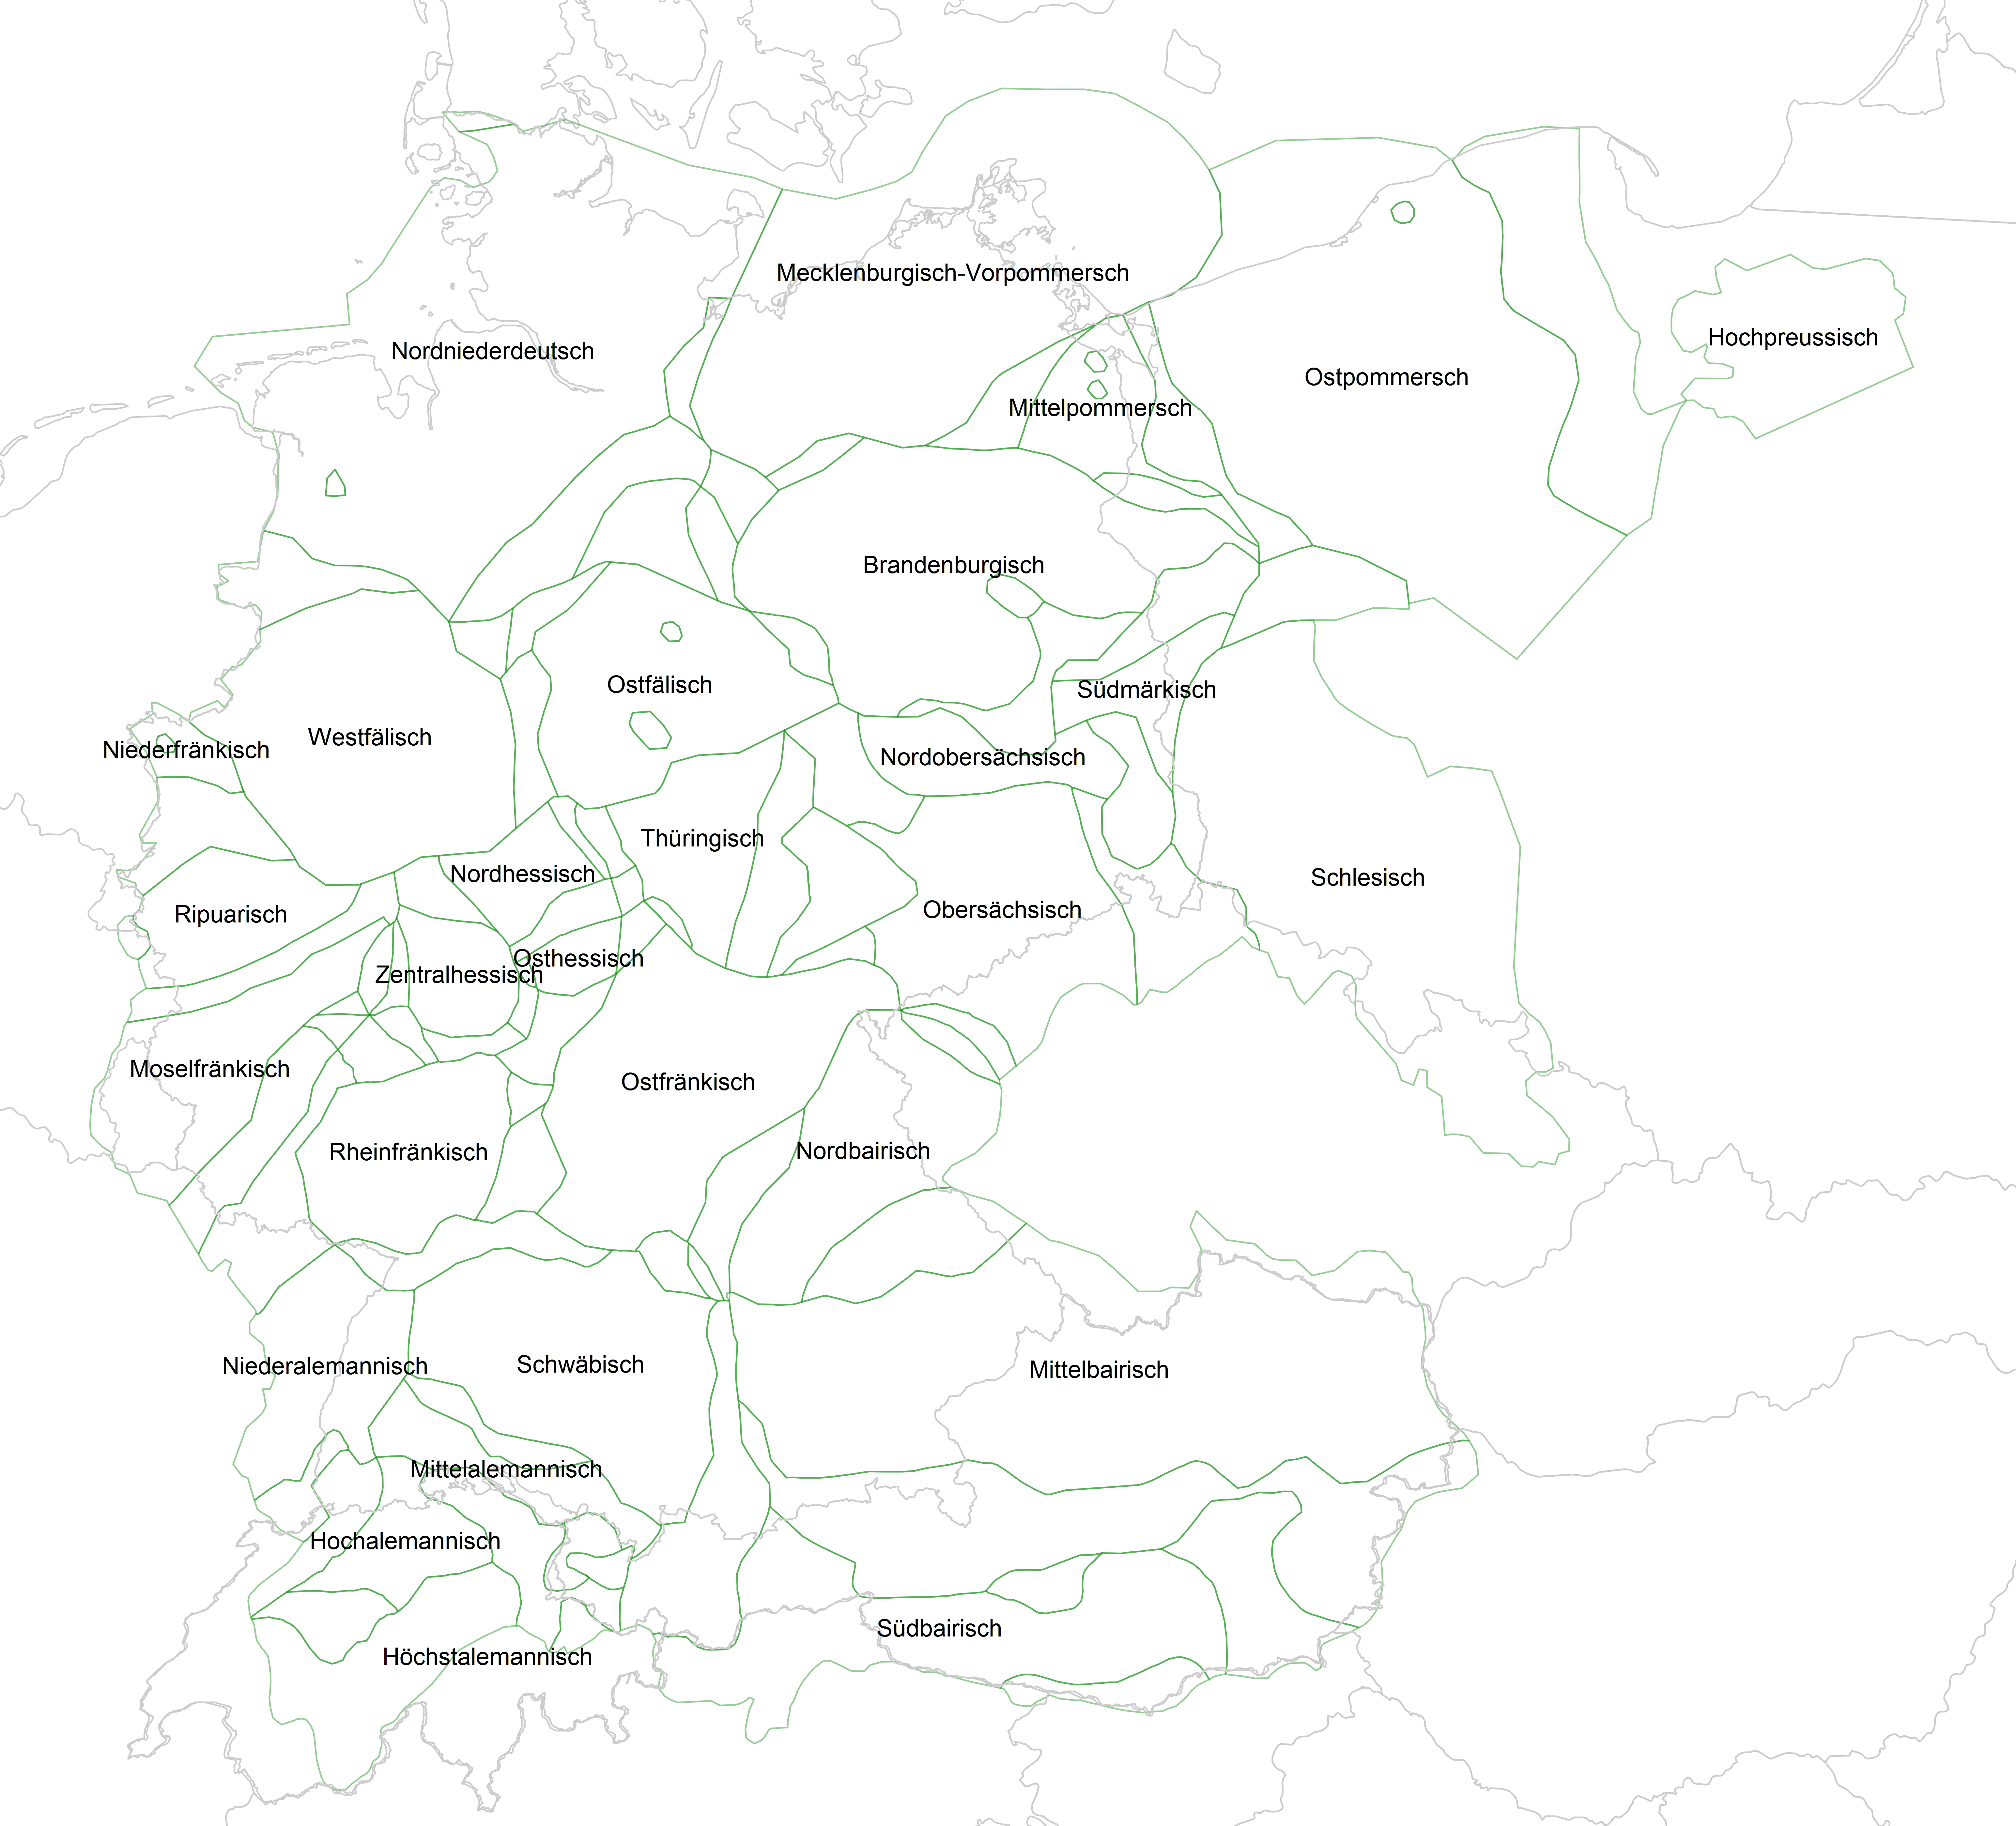
\includegraphics[width=\textwidth]{figures/WiesingerREDE2.png}
		\caption{\label{kartedtdialekte}Einteilung deutscher Dialekte (ohne Sprachinseln) nach \parencite[830, Karte 47.4]{Wiesinger1983a}; erstellt mit \url{www.regionalsprache.de/}}
	\end{figure}



\item Da der verwendete Dialektbegriff nicht in einer direkten Abhängigkeit zu einer \quein{Standardsprache} steht, ergibt sich auch ein in der deutschsprachigen Dialektologie eher unüblicher Standardbegriff. Als \quein{Standardsprache} wird zunächst nach Haugen (1994) jede schriftsprachliche Norm verstanden:

\begin{quote}
Any vernacular (language or dialect) may be \sem{standardized} by being given a uniform and consistent norm of writing that is widely accepted by its speakers. It may then be referred to as a \sem{standard} language. \parencite[4340]{Haugen1994}
\end{quote}

 
Diese Definition, die Aussprachenormen zunächst nicht mit einbezieht, ist besonders für die historische Perspektive sinnvoll, da wir bis in das \,%rs in das
20. Jahrhundert hinein von einer Parallelität von Dialekten und Schreibvarietäten ausgehen können. Die Entstehung einer überregionalen Schreibnorm, die zumeist auch nationalbildend wirkt, ist ein dynamischer Prozess. Das moderne Schriftdeutsche entwickelt \,%rs entwickelt 
sich ab dem 16. Jahrhundert (vgl.\, \citealt{Besch1988,Besch2003,Mattheier2000}). Für das (lange) 19. Jahrhundert als relevanten Zeitraum der vorliegenden Untersuchung kann man bereits von einer weitaus gefestigteren Schreibnorm ausgehen als in früheren Jahrhunderten; nichtsdestotrotz muss jedoch bedacht werden, dass der Standard des 19. Jahrhunderts noch in vielerlei Hinsicht ein im Vergleich zum Gegenwartsdeutschen \,%rs +en
des 21. Jahrhunderts inhomogenes, präskriptives \,%rs präskriptives
System darstellt (vgl.\, \citealt{Elspass2005a,Elspass2005}). Der Normbegriff der Autoren des (langen) 19. Jahrhunderts unterscheidet sich von der heutigen Form und Funktion präskriptiv genormter Register. Nach der Definition von Weiß (s.\,o.) macht die deutsche Standardsprache im Verlauf des 19. und frühen 20. Jahrhundert einen Wandel vom Typ \hai{N2} zum Typ \hai{N1} durch (vgl.\, \citealt[12f]{Weiss1998}). 


\item Die Einteilung jiddischer Dialekte folgt grundsätzlich derjenigen von \citealt{Katz1983}. Da die Katz'sche Einteilung der westjiddischen Dialekte durch kaum empirische Evidenz gestützt ist, nimmt diese Arbeit zur Verfeinerung des Dialektraums eine zusätzliche  Ost-West-Einteilung entlang des 9. Längengrads (Hamburg–Bregenz) vor.\label{BregenzHH} Diese Grenze verläuft entlang der \ili{bairisch}–alemannischen Sprachgrenze sowie der zwischen Ost- und Westmittel- \linebreak deutsch und der zwischen den west- und ostniederdeutschen Dialekten (vgl.\, \citealt{Wiesinger1983a}). 
% Damit orientiert sich diese Einteilung an den Raumstrukturen deutscher Dialekte, selbst wenn empirische Befunde zu einer solchen geographischen Gliederung des Westjiddischen bislang nicht erbracht werden konnten.
Damit orientiert sich diese Einteilung an den Raumstrukturen deutscher Dialekte, selbst wenn empirische Befunde zu einer solchen geographischen Gliederung des Westjiddischen bislang nur für den nördlichen Raum entlang der Elbe erbracht werden konnten (vgl. \citealt[209]{Ramer1997}). 
Daraus ergeben sich die westjiddischen Dialektregionen: 
westliches \ili{Südwestjiddisch} (westl. \hai{{\SWJ}}), 
östliches \ili{Südwestjiddisch} (östl. \hai{{\SWJ}}), 
westliches Zentral\ili{westjiddisch} (westl. \hai{{\ZWJ}}), 
östliches Zentralwest\-jid\-disch (östl. \hai{{\ZWJ}}), 
westliches \ili{Nordwestjiddisch} (westl. \hai{{\NWJ}}) und 
östliches \ili{Nordwestjiddisch} (östl. \hai{{\NWJ}}). 
Die Übergangsgebiete \ili{südliches Übergangsjiddisch} (\hai{{\SÜJ}}) und \ili{nördliches Übergangsjiddisch} (\hai{{\NÜJ}}) sowie die ostjiddischen Dialekte (Zentral\ili{ostjiddisch} ‏\hai{{\ZOJ}}, Süd\ili{ostjiddisch} \hai{{\SOJ}} u. \ili{Nordostjiddisch} \hai{{\NOJ}})  folgen weiterhin Katz (\citeyear{Katz1983}). 

%%%%Karte Dialekte%%%%
\begin{figure} 
\centering
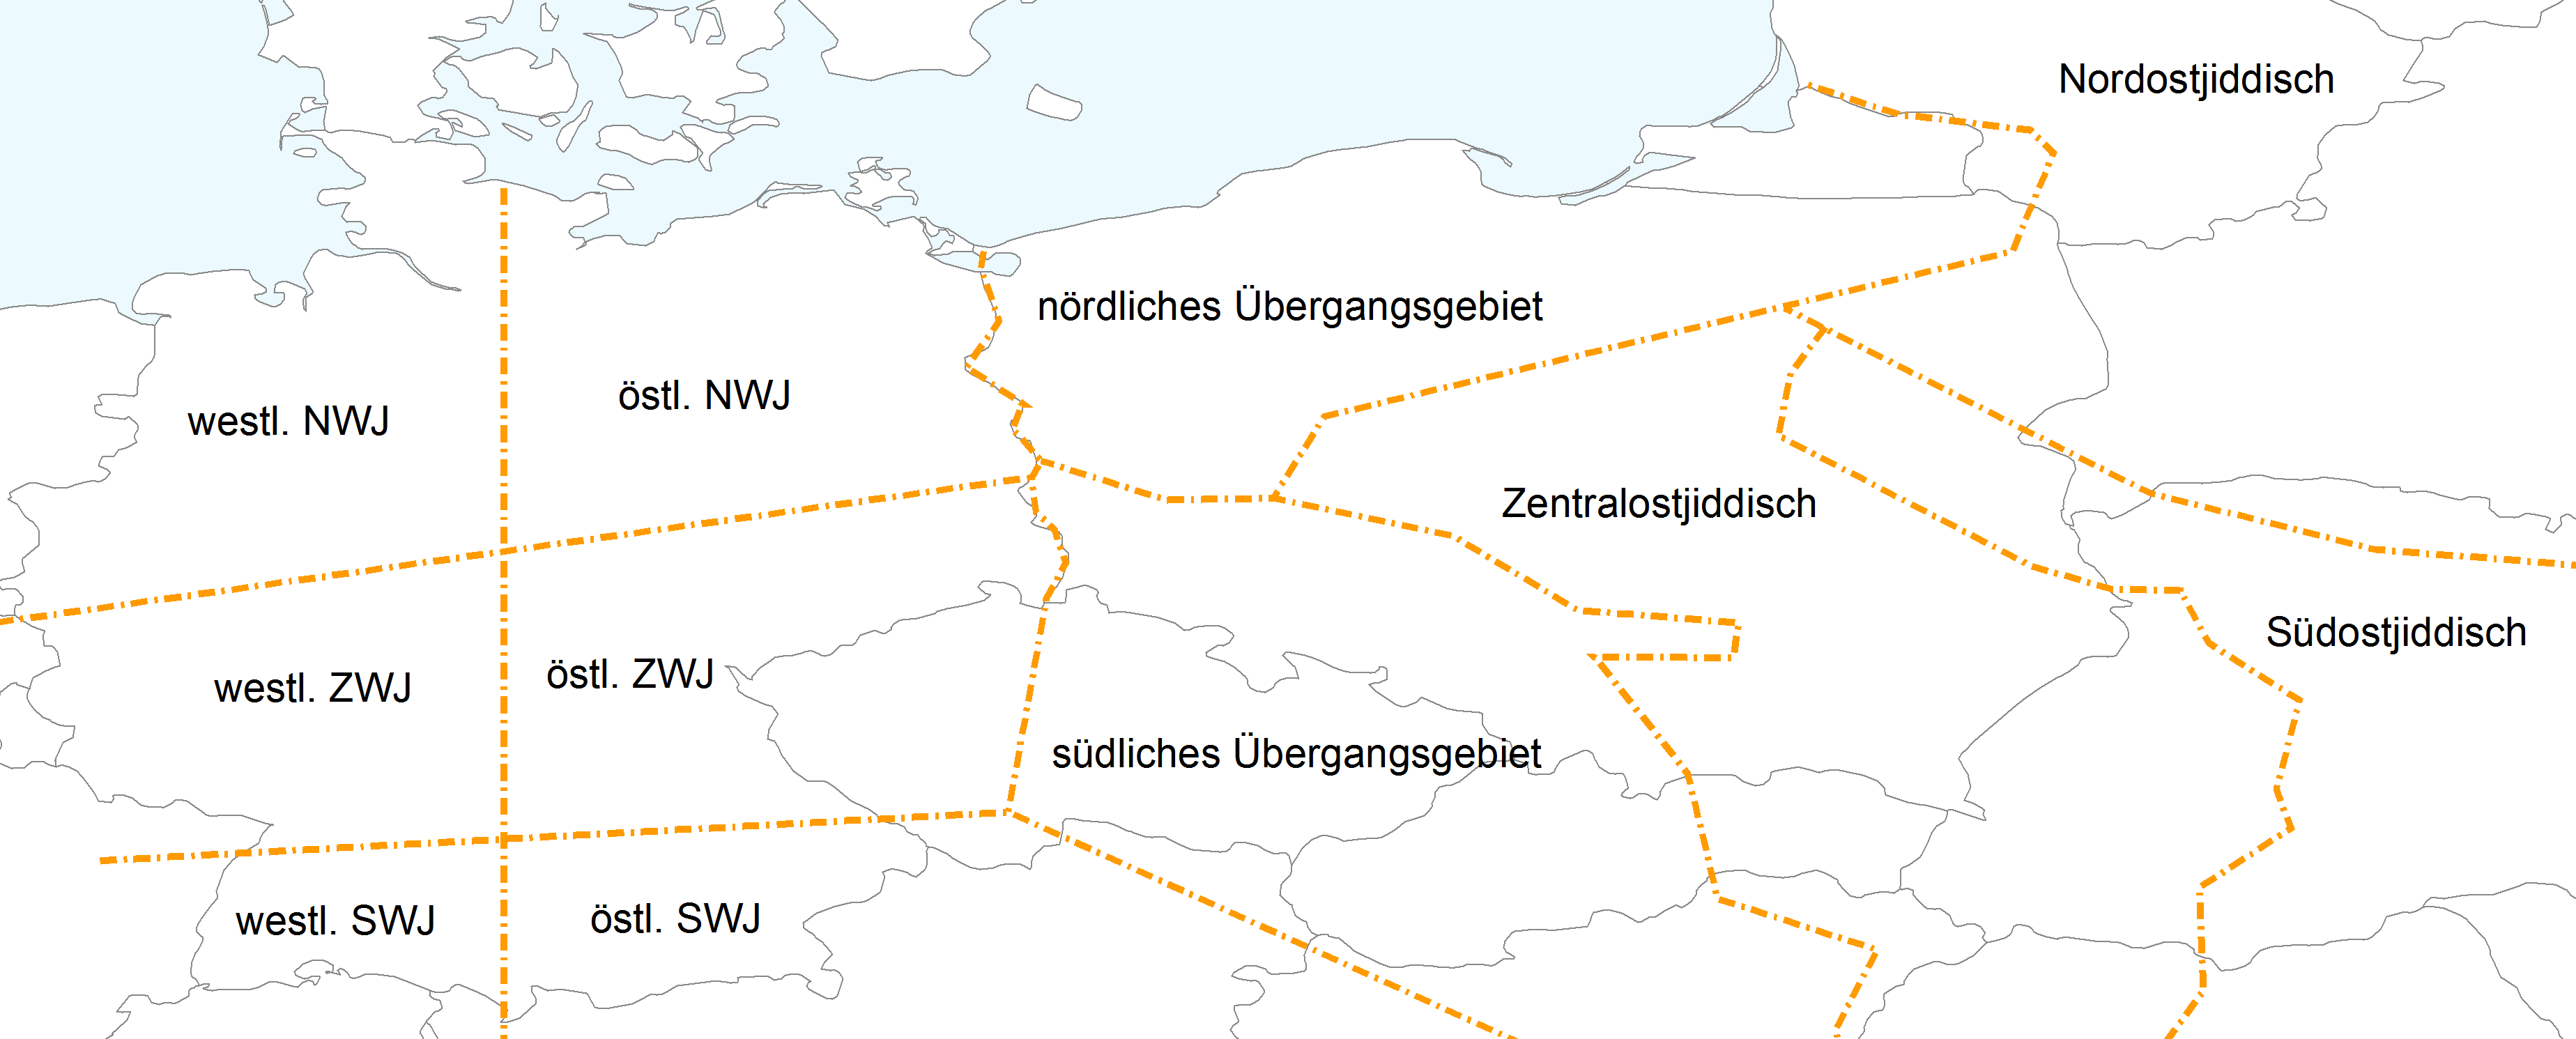
\includegraphics[width=\textwidth]{figures/regionen_diss_farbe2b.png}
		\caption{\label{karteregionen}Einteilung jiddischer Dialekte in Anlehnung an \cite{Katz1983}}
		\end{figure}
 
		%\clearpage

\newpage 	
\item Ein für diese Arbeit zentraler Begriff ist derjenige der \quein{Imitation}. Sprachliche \isi{Imitation} wird als genereller Oberbegriff für die Nachahmung einer Sprache durch einen Nicht-Muttersprachler verwendet. Die genauen Strategien, wie diese \isi{Imitation} vollzogen wird, beschreiben die Begriffe \quein{Emulation} und \quein{Simulation}. Im Falle der \isi{Emulation} wird die zu imitierende Sprache (target language, Zielsprache) in ein bestehendes Grundsystem (Grammatik) einer Matrixsprache eingebettet, adaptiert.\footnote{Der Begriff \quein{Matrixsprache} ist in Anlehnung an das \textit{matrix language frame model} (\hai{MLF}) nach 
\citeauthor{MyersScotton1993} (\citeyear{MyersScotton1993,MyersScotton2002}) gewählt, welches ein ideales Modell für die Grundstrukturen bilingualer Interferenzen wie code-switching 
oder code-mixing darstellt, indem es von einer asymmetrischen Opposition von \textit{matrix language} und \textit{embedded language} ausgeht. Sprachliche \isi{Imitation} ist insofern mit Bilingualismus vergleichbar, als dass ein Ausgleich zwischen zwei Sprachen stattfindet, in welchem eine Sprache (\textit{matrix language}) die Basis bildet, die entweder gezielt (emulierende \isi{Imitation}) oder spontan (code-switching) 
durch eine weitere Sprache (\textit{target language} oder \textit{embedded language}) manipuliert wird. Der größte Unterschied besteht darin, dass die in die Matrixsprache eingebundene Sprache im Fall von Bilingualismus vollständig beherrscht wird, im Fall der \isi{Imitation} jedoch bestenfalls einzelne Strukturen bekannt sind. Aus diesem Grund wird zwar Myers-Scottons (\citeyear{MyersScotton1993,MyersScotton2002}) Begriff der Matrixsprache adaptiert, auf eine Verwendung (und Eindeutschung) des Begriffs \textit{embedded language} wird aber  verzichtet. Es wird hier vielmehr die Terminologie Myers-Scottons verwendet, als ihr Modell. Es ist weiteren Arbeiten vorbehalten zu prüfen, \,%rs  prüfen,
ob die Mechanismen von sprachlicher \isi{Imitation} denen von code-switching/code-mixing folgen.\,%rs hier klein s.o.
} Die \isi{Simulation} einer Sprache hingegen erfolgt losgelöst von einem Grundsystem.
Die Graphiken in Abbildungen \ref{emulativgrafik}  und \ref{simulativgrafik} illustrieren den grundlegenden Unterschied zwischen simulierender und emulierender \isi{Imitation}. Im Fall sprachlicher \isi{Emulation} werden erkannte Strukturen der Zielsprache in das System der Matrixsprache integriert. Die sprachliche \isi{Simulation} hingegen integriert lediglich oberflächliche Strukturen der Zielsprache in das System der Matrixsprache und so treten Formen der Zielsprache losgelöst von einer sprachlichen Struktur auf. In anderen Worten: die \isi{Simulation} verfügt im Gegensatz zur \isi{Emulation} über keine zugrundeliegenden sprachlichen Strukturen, sondern besteht nur aus einzelnen, unzusammenhängenden Formen der Zielsprache. Die qualitative und quantitative Intensität der erkannten Formen wird in beiden Fällen durch einen Filter externer und interner Faktoren bestimmt, der zwischen Matrix- und Zielsprache besteht. Dieser Filter bestimmt die Qualität und Quantität der imitierten Strukturen und entscheidet letzten Endes darüber, welche der Imitationsstrategien (simulativ/emulativ) möglich ist. Er setzt sich aus den folgenden Faktoren zusammen: 
\begin{itemize}
\item [1.] Externe Einflüsse (z.\,B.\, Konzepte von Sprache, Pejorationen, erkannte grammatische Regeln, Intensität des Sprachkontakts) 
\item [2.] Typologische Nähe/Distanz von Matrix- und Zielsprache
\item [3.] Viskosität der Matrixsprache (\,= Potenzial sprachlicher Variabilität und Stativität) 
\end{itemize}
\label{emulationsbegriff}
 Zur weiteren Veranschaulichung helfen Beispiele aus der Architektur. Die sprachliche \isi{Simulation} ist als \quein{Potjomkinsche Dörfer} zu denken; sie ist eine sprachliche Attrappe. Die \isi{Emulation} hingegen kann man mit den Neo-Stilen (Neobarock, Neoromantik, Neorenaissance usw.) des 19. Jahrhunderts vergleichen: An eine moderne Bausubstanz werden Baustile einer anderer Epochen  angebracht, um Historizität zu evozieren. Die Zusammenhänge zwischen Matrix- und Zielsprache und den einzelnen Funktionen und Wirkungsweisen des \quein{Filters} werden im Unterabschnitt \ref{salienz} (ab S.\, \pageref{salienz}) näher ausgeführt. 


\begin{figure}[p]
 \begin{center}
 \begin{tikzpicture}
    \draw [fill=gray!20,opacity=0.7](0,1.5) circle (1) node[left=6.4ex] {\footnotesize Matrixsprache};
    \draw [->] (0.5,0.5) -- (1.3,-1);
    \draw [fill=gray!99,opacity=0.7](4,1.5) circle (1) node[right=6.4ex] {\footnotesize  Zielsprache};
        \draw [->] (3.5,0.5) -- (2.7,-1);
        \draw [gray, dashed] (0,-0.25) -- (4,-0.25) node[right] {\footnotesize  \textit{Filter}};
    \draw [fill=gray!60,opacity=0.7] (2,-2) circle (1) node[below=6.4ex] {\footnotesize  Imitat};

             \end{tikzpicture}
              \caption{\label{emulativgrafik}Modell emulativer Imitation}		
\end{center}
 \end{figure}



\begin{figure}[p]
 \begin{center}
 \begin{tikzpicture}
 \draw [fill=gray!60,opacity=0.7](0,1.5) circle (1) node[left=6.4ex] {\footnotesize Matrixsprache};
    \draw [->] (0.5,0.5) -- (1.3,-1);
    \draw [fill=gray!60,opacity=0.7](3, 0.5) rectangle (5,2.5);
 \node[opacity=0.7] at (6,1.5) {\footnotesize  Zielsprache};
          \draw [->] (3.5,0.45) -- (2.7,-1);
             \draw [gray, dashed] (0,-0.25) -- (4,-0.25) node[right] {\footnotesize  \textit{Filter}};
  %  \draw [fill=white!10,opacity=0.7] (2,-2) circle (1) node[below=6.4ex] {\footnotesize  Imitat};
\node[fill=gray!60] at (1.5,-1.5) {};
\node[fill=gray!60] at (2,-2) {};
\node[fill=gray!60] at (2.25,-2.25) {};
\node[fill=gray!60] at (2.5,-2.5) {};
\node[fill=gray!60] at (2.5,-1.5) {};
\node[fill=gray!60] at (2.5,-2) {};
\node[fill=gray!60] at (2,-1.5) {};
\node[fill=gray!60] at (2.75,-2.25) {};
\node[fill=gray!60] at (1.25,-2) {};
\node[fill=gray!60] at (2.75,-2) {};
\node[fill=gray!60] at (1.75,-2.25) {};

\filldraw[color=gray!60,opacity=0.7] (2.25,-1.75) circle (0.75ex);
\filldraw[color=gray!60,opacity=0.7] (1.625,-1.99) circle (0.75ex);
\filldraw[color=gray!60,opacity=0.7] (1.5,-2.5) circle (0.75ex);

\node[opacity=0.7] at (2,-3) {\footnotesize  Imitat};
             \end{tikzpicture}
              \caption{\label{simulativgrafik}Modell simulativer Imitation}	
\end{center}
 \end{figure}


\end{itemize}


\chapter{Forschungsstand}\label{forschungsstand}

In diesem Kapitel wird ein knapper Überblick des derzeitigen Wissensstands der zentralsten Entwicklungen des (West-)Jiddischen und Arbeiten zum Literaturjiddischen gegeben. Da die empirische Datenanalyse im Zentrum dieser Arbeit steht, wurde auf umfangreichere wissenschaftsgeschichtliche Ausführungen zur Jiddistik verzichtet.\footnote{Für den aktuellsten und übersichtlichsten Wissensstand zur Jiddistik seien \cite{AptrootGruschka2010} und für eine detailliertere Darstellung  \cite{Weinreich1973} zurate zu ziehen.}


\section{Übersicht zum Forschungsstand der (west-)jiddischen Sprachgeschichte}\label{westjiddistik}
 
Das wesentliche Charakteristikum des Jiddischen liegt in seiner relativ geringen territorialen Gebundenheit: Jiddisch \qu{was once a vast linguistic continuum, the largest European speech area next to Russian} (\citealt[7]{Weinreich1962}). Während die meisten Sprachen Europas durch politische und geographische Grenzen definiert sind, ist das Jiddische über den religionskulturellen Bund der aschkenasischen Bevölkerung bestimmt, der Diasporajuden Zentraleuropas. Nur wenige andere Sprachen sind so eng an ein ethnisches Konzept gebunden wie das Jiddische an das Judentum.  Wie alle jüdischen Diasporasprachen ist Jiddisch eine Sprache, die immer im Spannungsfeld mit koterritorialen Sprachen stand (vgl.\, \citealt{Spolsky2014}). Jiddische Dialektologie heißt damit auch immer \qu{bilingual dialectology} (\citealt{Weinreich1962}; vgl.\, auch die Arbeiten \citealt{Mieses1915} u. \citealt{Fischer1936}; s.\,a. Kapitel \ref{multilingualismus}, S.\, \pageref{multilingualismus}).

Die jüdisch-aschkenasische Kultur entwickelte sich ab etwa 1000 n.\,d.\,Z. im deutschen Sprachraum, wo \qu{infolge einer sprachlichen Verschmelzung} der mitgebrachten (semitischen und romanischen) Sprachen und mittelhochdeutschen Dialekten das Jiddische entstand (\citealt[1018]{Katz1983}). Jiddische Varietäten, die im Kontakt zu slawischen Sprachen standen (\ili{Ostjiddisch}), entlehnten aus diesen Sprachen zusätzliche Strukturen und Lexeme. In beiden Dialektgroßräumen (Ost- u. \ili{Westjiddisch}) wird aber die überwiegende Komponente des Jiddischen von einer Fusion mittelhochdeutscher Dialekte bestimmt. Dabei handelt es sich aber nicht um eine deutsche Varietät, sondern man muss dem Jiddischen von Beginn an sprachliche Autonomie gegenüber den Geber- und Kontaktsprachen zugestehen. \ili{Westjiddisch} ist im Gefüge der deutschen Varietäten ein eigenständiges sprachliches System: 

\begin{quote}Keine einzige jiddische Mundart deckt sich mit einer bestimmten deutschen Ma. [Mundart; L.S.], sondern das Jiddische ist ein Abklärungsereignis für sich. (\citealt[69; s.\,a. 53–56]{Weinreich1923}) 
\end{quote}

Unser sprachgeschichtliches Wissen über das Alt- und Mitteljiddische ist insbesondere der Forschungsleistung Erika Timms (Universität Trier) zu verdanken. Doch noch immer stehen systematische grammatische Beschreibungen des Alt- und Mitteljiddischen aus, die uns dabei helfen könnten, die älteren Sprachstufen des Jiddischen innerhalb der westgermanischen Sprachen des Spätmittelalters und der frühen Neuzeit zu verorten.\footnote{Hinzu kommt, dass auch unser Wissen über die Nachbarvarietät des Altjiddischen, das tatsächlich gesprochene Mittelhochdeutsch zum jetzigen Zeitpunkt noch äußerst gering ist (vgl.\, \citealt{Wegera2000}).} In der Schriftsprache kann ab frühneuhochdeutscher Zeit eine stärkere Auseinanderentwicklung zwischen Deutsch und Jiddisch beobachtet werden (\citealt{Timm1987b,Timm1991,Timm2005}). Es darf angezweifelt werden, dass diese auch die Mündlichkeit betraf, da sie lediglich Entwicklungen überregionaler Schreibvarietäten erfasst, nicht aber natürlicher Sprachen. Erst mit der nationalistischen und puristischen Sprachpolitik des 19. Jahrhunderts und besonders mit der \isi{Assimilation} des deutschen Judentums löst sich die jahrhundertealte Koexistenz zwischen jiddischen und deutschen Varietäten auf, was vielerorts den \isi{Sprachtod} des Westjiddischen bedeutet. Vereinzelt konserviert blieb die alte Sprachsituation bis ins 20. Jahrhundert hinein in den diglossisch ausgerichteten Gebieten des \hai{{\SWJ}} im Elsass, der Schweiz und daran angrenzenden Ortschaften Südbadens (vgl.\, \citealt[69]{Mieses1915}). Diesem Umstand verdanken wir den umfangreichsten Datenbestand westjiddischer Dialekte (s. Kapitel \ref{chap:quellenkapitel}, S.\, \pageref{chap:quellenkapitel}). 

Der \isi{Sprachtod} des Westjiddischen wird häufig – und analog zum angenommenen Einfluss der lutherschen Bibelübersetzung auf die Standardisierung des Deutschen (vgl.\, \citealt{Besch1999}) – auf Mendelssohns Übersetzung des Tanachs ins Schriftdeutsche mit hebräischen Lettern (1780–1783) und dessen Einstellung zum Jiddischen als einen \qu{Jargon} zurückgeführt (erstmals \citealt[159]{PiererLoebe1860}; \citealt[113–114]{Mieses1915}). Tatsächlich aber sind die Abläufe des jiddischen Sprachtods im deutschsprachigen Raum weitaus komplexer (\citealt[20–32]{Weinreich1923}) und bedürfen einer eingehenden sozialgeschichtlichen Untersuchung. Die Quellenlage zum späten Westjiddischen (vgl.\, Kapitel \ref{chap:quellenkapitel}, S.\, \pageref{chap:quellenkapitel}) spricht dafür, dass sich der Rückgang stufenweise und von Region zu Region abweichend im Laufe des 18., 19. und 20. Jahrhunderts vollzog (vgl.\, \citealt{GuggenheimGruenberg1973,Roemer2002}). 


\section{Linguistische Perspektiven auf Sprachimitation}\label{forschungsgeschichteimitation}
 
Die wissenschaftliche Beschreibung und Untersuchung sprachlicher Imitationen fand bisher in verschiedenen Teilbereichen der Linguistik statt. Besonders in der Spracherwerbsforschung nimmt der behavioristische Ansatz an, dass Erst- und Zweitspracherwerb durch \isi{Imitation} erfolgen (insbes. \citealt{Fraseretal1963,Uzgiris1981}; \citealt[291–294]{Tauten1997}; \citealt{Markham1997,LightbownSpada2006,MeltzoffMoore1977,MeltzoffMoore1983,MeltzoffMoore1989,MetzoffPrinz2002}). Eng verwandt hiermit sind Arbeiten aus dem Feld der Sprachevolution.
 Hier wird das Prinzip des \textit{vocal learning} (\sem{stimmliches Lernen}) als evolutionäre Grundvoraussetzung für sprachliche Kommunikation gesehen (vgl.\, u.\,a.\, \citealt{Fitch2010,HauserChomskyFitch2002,Petkov2012}).\footnote{Vom Menschen abgesehen, findet sich dieses bei Vögeln (u.\,a.\, \citealt{Lipkind2013}), Elefanten (\citealt{Poole2005}), Meeressäugern wie Walen und Robben (\citealt{JanikSlater1997,Ralls1985}) und im Ultraschallbereich bei Fledermäusen (\citealt{Boughman1998}) und Mäusen (\citealt{Arriaga2012}). Bei Primaten konnte bislang ein solches Verhalten nur unter starken Vorbehalten festgestellt werden (\citealt{Crockford2004,Petkov2012}).} Auf einer noch allgemeinneren Ebene sieht das (sozial-)kognitivistische Modell der \qu{Shared intentionality} (erstmals \citealt{Tomaselloetal1993}) von Michael Tomasello und Kollegen in den menschlichen Strukturen und Funktionen von \isi{Imitation} wesentliche Grundprinzipien für  menschliche Lernprozesse – insbesondere die des sozialen Lernens (u.\,a.\,  \citealt[123]{TomaselloCarpenter2007,Tomaselloetal2005,Carpenter2006,Uzgiris1981}). %Problematisch ist hier besonders die Trennung der Bereiche \textit{Sprache} vs. \textit{Musik} (vgl.\, \citealt{Fitch2006}), die z.\,T. graduell zwischen 
 

Durch die gegebene instrumentelle Messbarkeit der lautlichen Ebene ergibt sich, dass phonetische (z.\,T. auch phonologische) \isi{Imitation} bisher stärker untersucht wurde als etwa grammatische (etwa \citealt{Tilmanns2013,Reiterer2012,Nielsen2011,Babel2012}). Das Zusammenspiel aller sprachlicher Ebenen blieb bislang unberücksichtigt. So finden sich auch in den bereits vorhandenen Untersuchungen zu Dialekt- und Akzentimitation nahezu ausschließlich Daten dieser zugänglichen Ebene (etwa \citealt{Babel2011,Purschke2010,Neuhauser2012,Segerup1999,Dossey2012,Siegel2010}; \citealt[12–14, 40]{Trudgill2006}; \citealt{Adank2010}; \citealt[63, 75]{labov1972a}). Eine Ausnahme stellt ein Experiment von \textcite[310–334]{Labov1968_1} dar, wo die \isi{Imitation} eines syntaktischen Phänomens getestet wurde. In ihren \qu{Memory tests} bei  achtjährigen Jungen der sogenannten \textit{Thunderbirds}-Straßengang in New York 1967, untersuchten Labov und seine Kollegen die Spiegelung bzw. \isi{Imitation} der Versuchspersonen von Fällen, \,%rs komma
 in denen  satzfinale Kopulaverben ausfallen.  

In allen 
% bisherigen 
vorliegenden %\todo{bisherigen $\to$ vorliegenden}
Arbeiten wird Dialektimitation vorwiegend als Teilbereich soziolinguistischer (insbesondere Pejoration) oder wahr\-nehmungs\-psycho\-logischer (Salienz) Fragestellungen herangezogen. Wie in Kapitel \ref{lijisprachwissenschaft} (S.\, \pageref{lijisprachwissenschaft}) zu sehen ist, lassen sich Imitationsdaten variationslinguistisch in weiterer Hinsicht vielfach nutzen.


In dieser Arbeit wird erstmals der Versuch unternommen, Sprachimitationen systematisch in \,%rs in 
 den sprachlichen Ebenen Lexik, Phonologie, \isi{Morphologie} und \isi{Syntax}  zu untersuchen. Neu ist dabei der Ansatz, Imitationsdaten auf ihren Nutzen als sprachhistorische Quelle zu prüfen. 
 Von Belang sind hier weniger die psychologischen und neurologischen Grundabläufe, die bei sprachlicher \isi{Imitation} eine Rolle spielen, als vielmehr eine deskriptive Erfassung der grammatischen Elemente, die bei der \isi{Imitation} nah verwandter Varietäten manipuliert werden können. Und so ist auch  die sprachtypologische Perspektive auf Imitationen nah verwandter Varietäten ein Novum. Diese Arbeit betritt somit in vielerlei Hinsicht sprachwissenschaftliches Neuland.
 


\section{Mündlichkeit in der Schriftlichkeit}\label{schmuendlichkeit}

Eine besondere Herausforderung stellt der Datentyp selbst dar. Die dieser Arbeit zu Grunde liegenden Imitationsdaten des (West-)Jiddischen, stammen aus literarischen, zumeist dramatischen, Quellen. Poetische Texte stellen nicht den idealsten Datenquelltyp für linguistische Analysen dar. Zu stark ist ein möglicher Einfluss der poetischen Lizenzen. Vor allem historische Sprachstufen, wie z.B. das Westjiddische des 18. und 19. Jahrhunderts, sind aber zumeist in keiner anderen, \textit{besseren} Form überliefert als der literarischen. Hier gilt die Maxime von  \cite[11]{Labov2010}: \qu{making the best use of bad data}. Dies heißt in der Praxis, die durch poetische Lizenzen entstandenen Strukturen zu identifizieren und aus dem Datenset authentischer Strukturen zu eliminieren. Bei der vorliegenden Untersuchung ist die Situation allerdings anders. Hier stehen die poetischen Lizenzen selbst im Zentrum der Analysen.

Die Verschriftlichung von standardfernen Varietäten ist nicht im Konzept der neuhochdeutschen Schriftlichkeit angelegt. Wenn standardferne Varietäten innerhalb der Literatur auftreten, dann stehen sie immer im Gegensatz zu einer Standardsprache und wirken durch den Kontrast von Schriftlichkeit und Mündlichkeit. 

Es ist
wichtig, %\todo{add wichtig}
 hier zwischen dem \qu{Medium der Realisierung sprachlicher Äußerungen} und der \qu{Konzeption, die die Äußerungen prägt} zu unterscheiden (\citealt[587]{kochoesterreicher1994}). Wenn zum Beispiel ein Dialekt im Rahmen literarischer Figurenrede \,%rs kein Komma
als eine orale Varietät \,%rs kein Komma
verschriftlicht wird, dann ist er vom Medium her schriftlich. Er bleibt dabei aber von der Konzeption her mündlich, ist also nach \cite{KochOesterreicher1985} konzeptionell mündlich. Den Rahmen für konzeptionelle Mündlichkeit innerhalb der medialen Schriftlichkeit literarischer Texte bildet zumeist die direkte Rede. Als Quelle historischer Mündlichkeit eignen sich damit besonders Prosadramen,  wie es z.\,B.\, \textcite{Vosberg2016} am Beispiel einer Analyse von morphosyntaktischen Sprachwandelphänomenen des Englischen bestätigt.

Die hier zu analysierenden Auszüge aus der Figurenrede jüdischer Charaktere sind keine dokumentarischen Aufzeichnungen des gesprochenen Jiddischen, sondern auf Laienwissen fußende Emulationen der Sprache der Autoren (Deutsch) mit eigenen literarischer Funktionen (vgl.\, Kapitel \ref{Kapitel Funktionstypen}). 

Wie genau sprachliche Variation in der Literatur wirkt, dafür liefert Mikhail Bakhkin ein literaturwissenschaftliches Modell. Die unterschiedlichen Sprechlagen und grammatische Möglichkeiten einer Sprache nennt Bakhkin \textit{Heteroglossia}. Diese fließt in einen literarischen Texte ein und  bewirkt einen Diskurs der unterschiedlichen Sprechweisen (\textit{double-voicing}):

\begin{quote}
Heteroglossia, once incorporated into the novel (whatever the forms for its incorporation), is \textit{another's speech in another's language}, serving to express authorial intentions but in a refracted way. Such speech constitutes a special type of  \textit{double-voicing discourse}. It serves two speakers at the same time and expresses simultaneously two different intentions: the direct intention of the character who is speaking, and the refracted intention of the author. In such discourse there are two voices, two meanings and two expressions. \cite[324]{Bakhtin1981}
\end{quote}

\noindent \cite[u.\,a.\, 279, 285, 369, 418]{Bakhtin1981} betont wiederholt, dass ein literarisches Werk erst durch seine internen Dialoge wirkt.\footnote{In der Übersetzung ist hier die Rede von der 
% \textit{Power} 
\qu{Power}
eines Werkes} %\todo{Power nicht kursiv, sondern in ``''} 
Es sind die Abweichungen von der Norm, die poetischen Lizenzen, die einem literarischen Text sprachliche Dynamik verleihen. Die jüdische Figurenrede in der deutschen Literatur ist dafür ein äußerst prägnantes Beispiel. Die große Popularität dieses Stilmittels fußt auf der einfachen und direkten Wirkung, die sprachliche Variation im Rahmen einer sonst normierten Sprache hat. Losgelöst vom Inhalt des Gesagten tritt die Form ins Zentrum und wird somit zum Thema selbst.

 Solche Prinzipien machen sich Texte zu nutzen, die Formen des Literaturjiddischen verwenden. Vor allem im 18. und 19. Jahrhundert haben wir es hier mit Texten zu tun, die nicht in den literarischen Kanon aufgenommen sind und die wenig Komplexität und inhaltliches Gewicht aufweisen. Die Verwendung einer nicht normgerechten Sprache bei jüdischen Charakteren ist zumeist das einzige komische Element dieser Texte. Die Darstellung konzeptioneller Mündlichkeit fungiert hier ähnlich \,%rs kein Komma
 wie das stilisierte \textit{Türkendeutsch} in der Medien- und Jugendkultur der 1990er und frühen 2000er Jahre als \qu{eine Art \textit{fun-code}} (vgl.\, \citealt[59]{Deppermann2007}; \citealt{Auer2003}). Doch \ili{Literaturjiddisch} geht über die humoristische Funktion hinaus. Verwendet von nicht-jüdischen Autoren kann es z.\,B.\, auch identitätsschaffend, nostalgisch wirken (mehr dazu in Kapitel \ref{Kapitel Funktionstypen}).


\chapter{Literarische Traditionen}\label{lijiliteraturwissenschaft}


%\epigraph{\textit{A Huhn, wos kräjt, un a Goi, wos schmusst jiddisch – sollen sein Kapore far mir.}}{--- \textup{Jiddisches Sprichwort (\citealt[524]{Landmann2013})}} 
\largerpage

\noindent Aus der Literaturwissenschaft, insbesondere aus dem Forschungsfeld des literarischen Antisemitismus, liegt uns eine Reihe an Arbeiten zur jüdischen Figurensprache in der deutschsprachigen Literatur vor (insbes. \citealt{FischerBayerd2008,Kremer2007,Schreuder2002,Krobb2000,Glasenapp1999,Gubser1998,Groezinger1998,Richter1995,Och1995,Frey1994,Frey1992,Althaus1981,Althaus1986,Gelber1986,Denkler1977,Jenzsch1974}; erste Ansätze finden sich bereits bei \citealt{Carrington1897}). Dieser Abschnitt zeigt die zentralen Tendenzen auf, die sich aus dem literaturwissenschaftlichen Diskurs für das Literaturjiddische in seinem Verhältnis zum Jiddischen ergeben. Dabei wird der Blick vom Jiddischen in der deutschsprachigen Literatur auf den Umgang mit jüdischen Sprachen generell ausgeweitet. Sinn und Zweck dieses Abschnittes ist es, in einem Überblick die verschiedenen Reflexe, die jüdische Sprachen in literarischen aber auch filmischen Kunstwerken hinterlassen haben, darzustellen.  


\section{Die Sprache jüdischer Figuren als Topos der europäischen Literaturen}\label{euroliji}
%jüdische sprache in anderen literaturen
 
Jüdische Diasporasprachen stehen immer in einer Kontrastbeziehung zu koterritorialen Sprachen. Im Literaturjiddischen wird diese Beziehung literarisch realisiert. So ist es nicht überraschend, dass die besondere jüdische Sprachsituation auch in anderen Literaturen als der deutschsprachigen thematisiert wird. Hebt man die Beschränkung auf die jiddische Sprache auf, so lässt sich in der europäischen Literatur etwas finden, was man als \quein{Literaturjüdisch} bezeichnen kann, da oftmals jüdische Figuren sprachlich markiert werden, jedoch nicht über die jiddische oder hebräische Sprache, sondern über ein generelles \quein{Anders-Sprechen}. Solche Markierungen finden sich zum Beispiel in der
\il{niederdeutsch}niederdeutschen,
\il{dänisch}dänischen,
\il{englisch}englischen, 
\il{polnisch}polnischen  und 
\il{französisch}französischen  Literatur. %format! indizes verursachen leerschlag!!!

In der englischen Literatur kann in den Stücken Marlowes und Shakespeares eine unterschiedliche Sprechweise jüdischer Figuren festgestellt werden (\citealt[193]{Groezinger1998}). Ebenso in Werken des 19. Jahrhunderts, z.\,B.\, von Charles Dickens oder George Eliot (vgl.\, \citealt[193]{Groezinger1998}). Die Thematisierung des Jiddischen selbst tritt m.\,W. jedoch erst ab dem 20. Jahrhundert in der anglo-amerikanischen Literatur in Erscheinung (vgl.\, \citealt{Fischer2003}). Wie genau sich die Entwicklung der sprachlichen Markierungen jüdischer Figuren hier gestaltet, bedarf noch detaillierterer Analysen.

In einer anderen germanischen Sprache, nämlich dem Dänischen, finden sich Hinweise dafür, jüdische Figuren über die deutsche Sprache zu charakterisieren. So etwa im  Theaterstück \qu{Det Arabiske Pulver} (1724) von Ludwig Holberg, in dem die jüdische Rolle dadurch von den übrigen abgegrenzt wird, dass sie Hochdeutsch spricht.

\largerpage
\cite[60]{Hausmann1989} zeigt, dass in der Literatur Balzacs Elsässer und niederländische Juden in ihren Spracheigenschaften auffällig gestaltet sind. Die Judenfigur spricht hier \qu{schlecht französisch} und \qu{kauderwelscht […] mit stark germanischem Akzent} (\citealt[194]{Groezinger1998}). Auch hier fehlen umfassendere Analysen, um festzustellen, wie \quein{germanisch} die sprachlichen Formen tatsächlich sind und ob womöglich Imitationen des Jiddischen vorliegen.

Andere Beispiele jüdischer Figurenrede finden sich in der polnischen, tschechischen und russischen Literatur, in der Juden durch eine auffällige Aussprache der jeweiligen Landessprache charakterisiert werden (insbes. \citealt{Brzezina1986,Berger1999,Kosta1999,Dohrn1999}; \citealt[194–196]{Groezinger1998}). Diese phonetischen Besonderheiten können selbstverständlich auch auf Interferenzen mit dem Jiddischen zurückzuführen sein. Eine diese Hypothese überprüfende Analyse steht noch aus. 

Besonders interessant sind hier die zwei tschechischen
Theaterstücke \qu{Čech a Němec} \sem{Der Tscheche und der Deutsche} (Jan Nepomuk Štěpánek, 1816) und \qu{Fidlovačka aneb Žádný hněv a žádná rvačka} \sem{Das Schusterfest oder keine Wut und kein Lärm} (Josef Kajetán Tyl, 1834).\footnote{Den Hinweis auf diese Stücke verdanke ich Agnes Kim (Universität Wien), die mir auch bei der Übersetzung des Textausschnitts zur Seite stand.} Diese beiden Stücke thematisieren die deutsch-tschechische Mehrsprachigkeit direkt über die Figurenrede. Die darin auftretenden jüdischen Figuren (Aron u. Šiveles) zeichnen sich dadurch aus, dass sie in dieser Mehrsprachigkeit perfekt eingegliedert sind. Sie sprechen neben kürzeren tschechischen Phrasen \,%rs kein Komma
hauptsächlich deutsch; allerdings ein leicht markiertes Deutsch, \,%rs groß
das \,%rs welches
an das \hai{{\LiJi}} deutschsprachiger Autoren erinnert: 

\begin{quote}

Aron: Was heißt das? bin ich doch erschrocken, dass ich habe geglaubt, ich kriege die Frais. Und es ist doch nichts gewesen als das Echo. Nu, tedy musím jen hledět tu škatulku někde schovat a místo si pamatovat. \\ 
{\sem{\small{$[$…$]$ Nun, also muss ich nur noch zusehen, dass ich diese Schatulle irgendwo verstecke und mir den Ort merke.}} }\\
(\qu{Čech a Němec} 1816: 6)

\end{quote}

Wie die Analysen in Teil \ref{analysen} (S.\, \pageref{analysen}) dieser Arbeit zeigen, entsprechen die hier auftretenden Abweichungen vom Schriftdeutschen \,%rs -en
den Strukturen, die im deutschen \hai{{\LiJi}} besonders frequent sind. Ich erlaube mir kein Urteil darüber, ob und inwiefern auch das Tschechisch der jüdischen Figuren von der tschechischen Norm abweicht.\footnote{Einer ersten Einschätzung der Slawistin \,%rs groß
Agnes Kim (Universität Wien) zufolge sind besonders in der  tschechischen Sprache der jüdischen Figur Šiveles Abweichungen von der Norm zu erkenennen.} 

Auch in der niederländischen Literatur des 19. Jahrhunderts sind Tendenzen zu erkennen, jüdische Figuren sprachlich zu markieren. Dies findet sich etwa in der Sprache des Juden Simon im Stück \textit{De lotgevallen van Ferdinand Huyck} von Jacob van Lennep (1840)\footnote{Den Hinweis auf diese Quelle verdanke ich Marion Aptroot.} oder der Figur des Moses Nathan im antisemitischen Text anonymer Autorschaft \qu{Een Christen, die een Jood had bedrogen: blijspel voor rederijkers in 3 bedrijven} (1867). Hier spielt aber weniger das niederländische Nordwestjiddische eine Rolle. Vielmehr finden sich phonologische Manipulationen am Niederländischen selbst, mit denen eine den Juden eigentümliche Art und Weise der Aussprache der Landessprache (\textit{Judeo-Dutch}; vgl.\, Kap.\, \ref{multilingualismus}, S.\, \pageref{multilingualismus}) evoziert wird. Besonders zentral sind hier Aspirierungen wie \textit{dhat} vs. {\ndl} \textit{dat} \sem{das(s)} (\qu{Een Christen, die een Jood had bedrogen}:\,41) oder \textit{thock} vs. {\ndl} \textit{toch} \sem{doch} (\qu{Een Christen, die een Jood had bedrogen}:\,44). Aber auch lexikalische Marker, wie etwa mit Ausdrücken wie \textit{Awhaai!} \sem{Ohweh!} (\qu{Een Christen, die een Jood had bedrogen}:\,42), spielen eine zentrale Rolle. Ob und inwiefern diese Darstellung der Sprachrealität entspricht, bleibt weiteren Analysen überlassen. Bezeichnend ist, dass sich die niederländische Literatur mit ihren Strategien der jüdischen Figurenrede größtenteils deutlich vom Literaturjiddischen der deutschen Literatur unterscheidet. Eine interessante Ausnahme stellt die 1834 in Amsterdam erschienene Ausgabe der \textit{Gedichter, Parabeln unn Schnoukes} (\hai{GP} Nürnberg, 1831) Itzig Veitel Sterns (Pseud.) unter dem Titel \qu{Gedichten, Parabelen en Sjnoekes of poëtische paarlensnoer voor de Kalle. Eene Rariteit van Itzig Feitel Stern} dar (vgl.\, Abschnitt \ref{IVS}, S.\, \pageref{IVS}).

 
In der niederdeutschen Literatur des 19. Jahrhunderts finden wir hingegen jüdische Figurenrede, wie sie aus der hochdeutschen Literatur bekannt ist. Die vorliegende Arbeit analysiert erstmals einige solcher Quellen (vgl.\, die Quellen \hai{UT} Stavenhagen, 1862; \hai{DP} Pyrzyce, 1874 u. \hai{DK} Osterwieck, 1872). Hier mag der etwas größere sprachliche Abstand, also die typologische Distanz, zwischen Jiddisch und Niederdeutsch als die zwischen Jiddisch und Hochdeutsch unterschiedliche Muster der \isi{Imitation} generieren.

  
Generell lässt sich festhalten, dass ein typologischer Vergleich der Imitationsmuster jüdischer Sprachen und insbesondere des Jiddischen in den europäischen Literaturen ein interessantes Forschungsunterfangen darstellen würde. Bislang konnte jedoch nur in der deutschsprachigen (hoch- und niederdt.) Literatur eine in alle sprachliche Ebenen der Matrixsprache eingreifende fiktionale Sprache jüdischer Figuren gefunden werden. Das besondere Verhältnis zwischen Deutsch und Jiddisch, welches in der gemeinsamen {\mhd} Komponente begründet ist, ermöglicht ein gegenseitiges Verständnis und schafft erst die Möglichkeit zur \isi{Emulation} der anderen Sprache. So kann in etwa auf phonologischer Ebene eine Lautregel des Jiddischen (z.\,B.\, {\mhd} \textit{ê} > /ei/) auf deutsche Lexeme angewendet (emuliert) werden (z.\,B.\, \textit{geihn}  \sem{gehen}, \textit{steihn} \sem{stehen}), um den Eindruck des Jiddischen zu erwecken. Die Rekonstruktion eines deutschen Wortes oder einer deutschen Struktur aus einer literaturjiddischen Form ist für einen Muttersprachler des Deutschen noch immer möglich, womit die Verständlichkeit garantiert ist. Dagegen können andere Sprachen, wie etwa Englisch oder Französisch, nur mehr in einzelnen Ebenen jüdische Sprachen emulieren, sofern eine inhaltliche Verständlichkeit für die Leserschaft erhalten bleiben soll.



\section{Literaturhebräisch in der deutschsprachigen Literatur}\label{lihe}
%%lihe
  
Bereits vor dem 18. Jahrhundert finden sich in der deutschsprachigen Literatur eine dem Literaturjiddischen ähnliche literarische Strategie der Charakterbildung  
jüdischer Figuren, jedoch auf Grundlage \,%rs auf Grundlage
einer anderen jüdischen Sprache: des Hebräischen.  \cite[8]{Carrington1897} beschreibt dieses \hai{Literaturhebräisch} (\hai{{\LiHe}}) anhand eines Innsbrucker Osterspiels aus dem 14. Jahrhundert als \qu{unverständliche[s] Gemisch von lateinischen und verdrehten hebräischen Wörtern}. \cite[197]{Frey1994} bezeichnet \hai{{\LiHe}} schlichtweg als \qu{Kauderwelsch}. Die ideologisch höchst problematische Arbeit Frenzels (\citeyear[24]{Frenzel1942}) nennt es \qu{Pseudo-Hebräisch}.

\largerpage
\citeauthor{Frey1992} (\citeyear{Frey1992}) zeigt, dass \hai{{\LiHe}} ganz unterschiedliche Formen annehmen kann. Es finden sich Stücke, welche mit der unverständlichen Anhäufung \ili{hebräisch} (und ggf. lateinisch/ \ili{italienisch}) klingender Wörter arbeiten (\ref{bsplihe1}),\footnote{In den Lexemen \textit{calsim}, \textit{calcasim} und \textit{tripsim} lässt sich sogar das hebräische \isi{Pluralsuffix} der Maskulina -\textit{im} erkennen. In diesem Fall ließe sich sogar von der \isi{Emulation} des hebräischen Suffixes im Rahmen einer \isi{Simulation} sprechen.} von denen nur wenige Elemente einen klaren Wiedererkennungswert zum Hebräischen haben. Diese sind wie in (\ref{bsplihe1}) vorrangig \isi{Eigennamen} des Alten Testaments (\textit{abraham} \sem{Abraham}, \textit{moyses}\footnote{Hier sogar mit der aschkenasischen (vorwiegend ostjiddischen) Diphthongierung von /o\textlengthmark/ > /ɔj/.} \sem{Moses}, \textit{jacob} \sem{Jakob}) oder aber auch einer der populäreren jüdischen Gottesnamen (\textit{adonay} \sem{Herr}). Andere Stücke arbeiten mehr mit einem Gemisch aus Deutsch und Phantasiephrasen, die etwas Beschwörungshaftes an sich haben (\ref{bsplihe2}). Auf diesem Weg kann der Text nicht nur über die unverständlichen Elemente, sondern auch über den Inhalt der verständlichen Passagen Juden diffamieren. \citeauthor{Frey1992} (\citeyear[62]{Frey1992}) findet nur in einem einzelnen Text tatsächliches Hebräisch, das zur Figurencharakterisierung gebraucht wird. Hierbei handelt es sich um das \RL{{{א\makebox(-1.25,-1.15)[r]{\libertineGlyph{uni05B7}}}}ד{\makebox(0,9)[l]{\libertineGlyph{uni02D9}}{ו}}ן ע{\makebox(0,9)[l]{\libertineGlyph{uni02D9}}{ו}}{ל\makebox(-1.15,-1.15)[r]{\libertineGlyph{uni05B8}}}ם} \sem{Herr der Welt} aus dem \RL{שחרית} \textit{Shakharit} (jüdisches Morgengebet) (\ref{bsplihe3}). Im Stück selbst wird anschließend an den \qu{hebräischen} Vortrag der Text direkt ins Deutsche übersetzt wiedergegeben (\citealt[62]{Frey1992}). Doch eine solche beinahe aufklärerische Verwendung des Hebräischen ist in den Passionsspielen eine Ausnahme. 

 \eenumsentence{
	\item \textit{Schïroli kakma nedana scharobora ka lankato waycheilo gawidello in dezbro abraham vnd moyses jacob kadakados adonay sebeos calsim calcasim tripisim calca} […] \\(Erlauer Spiele; Anfang 15. Jh.; zit. nach \citealt[59]{Frey1992})
\label{bsplihe1} 

\item \textit{Dar umb so nemmend wir dafür \\ Brad würst vnnd sure senff, \\ ist aller Juden tämpf, \\ gammahü mahü. \\ Alla calla malla, \\ Alla willa wigrui \\ rui rui pfu pfu!} […] \\(Luzerner Osterspiel; Mitte 15. Jh.; zit. nach \citealt[68]{Frey1992})
\label{bsplihe2} 

\item \textit{Adan holana ascher molach pethorem \\ Koll jhetzir niffra bohot nathase be \\ Hefizo kol asahi meloch schemonicra} […] \\(Hanz Folz \qu{die alt und neu ê}; Ende 15. Jh.; zit. nach \citealt[59]{Frey1992})
\label{bsplihe3} 
}


Abgesehen von dem aus dem Rahmen fallenden Text in (\ref{bsplihe3}) wird in den Passionsspielen Hebräisch simuliert, nicht emuliert. Es findet sich nie eingebettet in einen sprachlichen Rahmen. 


\hai{{\LiHe}} funktioniert damit anders als \hai{{\LiJi}}: Jeder Autor hat beim ersteren sein eigenes Konzept, wohingegen im Fall des \hai{{\LiJi}} gemeinsame Strukturen gegeben sind. Das \hai{{\LiJi}} emuliert das Jiddische mit Deutsch als Basis, das \hai{{\LiHe}} simuliert hingegen mit Hilfe einzelner kennzeichnender Wörter (\textit{adonay}), v.‏\,a. aber über bedeutungslose Lautansammlungen das Hebräische. Bei beiden Formen der \isi{Imitation} ist Deutsch die zugrunde liegende Sprache. Literarische \isi{Imitation} kann demnach verschiedenen Strategien folgen.

Ab welchem Zeitpunkt \hai{{\LiHe}} auftaucht, ist nicht klar zu beantworten. Den Arbeiten Freys (\citeyear{Frey1992,Frey1994}) liegen Texte aus dem 15. und 16. Jahrhundert zugrunde. Auch \citeauthor{Carrington1897} (\citeyear{Carrington1897}) gibt nicht an, ab wann die Sprache zum Thema der jüdischen Figuren wird. Sein frühestes Beispiel für eine Quelle des \hai{{\LiHe}} stammt aus dem 14. Jahrhundert (\citealt[7f]{Carrington1897}). Er nennt allerdings bereits Hinweise für eine besondere Gestaltung jüdischer Rollen im 12. Jahrhundert:
\begin{quote}
In den geistlichen Spielen finden wir sehr früh die Juden als komisches Element verwendet. Schon im XII. Jahrhundert beklagen sich einzelne Geistliche darüber, und in den folgenden Jahrhunderten nimmt das Gefallen der Zuschauer an diesem Elemente bedeutend zu. Gegenstand der Verspottung sind vor allem Schacher und Wucher, Sprache und Gesang. (\citealt[7]{Carrington1897})
\end{quote}

In einem Benediktbeurer Weihnachtsspiel findet sich ein Hinweis auf eine mimische und gestische Markierung jüdischer Figuren in einem Stück des 13. Jahrhunderts:

\begin{quote}
Archisynagogus cum suis Judeis valde obstrepit auditis prophetiis et dicat trucendo socium suum, movendo caput suum et totum corpus et percutiendo terram pede, baculo etiam imitando gestus Judei. (Benediktbeurer Weihnachtsspiel, 13. Jh.; zit. n. \citealt[260f]{Stumpfl1936}; bereits in \citealt[175]{Young1933}) \\

\footnotesize{Der Synagogenvorsteher lärmt mit seinen Juden gegen die gehörten
Weissagungen an und redet auf seinen Gefährten ein, indem er ihn
anstößt, seinen Kopf und seinen ganzen Körper schüttelt, mit dem Fuß auf
den Boden stampft, auch mit dem Stock die Gesten des Juden imitierend. (Übersetzung nach \citealt[473 Fn.,\,213]{Freise2002})}


\end{quote}

Die besondere dramatische Darstellung jüdischer Figuren geht demzufolge auf eine längere Tradition geistlicher Stücke zurück (vgl.\, \citealt[437]{Freise2002}). Die Manipulation der Sprache ist demzufolge, wie im \hai{{\LiJi}} nur ein dramaturgisches Mittel unter vielen. Weitere übliche Elemente finden sich im Bühnenbild, wie etwa der Einsatz der Farbe Gelb, des sog. \quein{Judenhuts} (\citealt[55–57]{Frey1992}) oder auch in der Verwendung (simulierter) hebräischer Quadratschrift, die auch über das Passionsspiel hinaus schon früh als Identifikationsmittel dienen (vgl.\, Abbildung \ref{judeneid}).\footnote{Diese Strategie zur Kennzeichnung jüdischer Figuren findet sich noch bis heute in filmischen und graphischen Darstellungen von Judenfiguren (vgl.\, Abschnitt \ref{fiji}).}\,%rs Punkt zuviel
 

\begin{figure}[h!]
\centering

\includegraphics[width=\textwidth]{figures/judeneid_ausschnitt.png}
		\caption{\label{judeneid} Darstellung eines sog. \quein{Judeneids}: Der Schwur auf den Tanach. Ausschnitt aus einem Holzschnitt des Augsburger \qu{Laienspiegel} (1509) mit hebräischen Lettern (entnommen aus \citealt[851]{Wolf2003})} 
		\end{figure}



Es ist ein Forschungsdesiderat, die überlieferten Textzeugen und ihre Strukturen und Funktionen des \hai{{\LiHe}} zu erfassen. Bislang liegt eine Reihe von Arbeiten zu Judenfiguren in spätmittelalterlichen Schauspielen vor (\citealt{Carrington1897}; \citealt[28--29]{Lowack1905}; \citealt{Bremer1986,Frenzel1942,Frey1991,Frey1992,Frey1994,Wenzel1992,Rommel2002,Freise2002,Mikosch2010}). Allerdings geht nur \citet{Frey1992,Frey1994} näher auf die Sprache jüdischer Rollen ein.

Die Tradition des \hai{{\LiHe}} muss bis ins 17. Jahrhundert hinein ein populäres Mittel der Dramatik gewesen sein.\footnote{\cite[10]{Carrington1897} nennt als letzte Quelle Andreas Gryphius Stück \qu{Horribilicribrifax} (1663). \cite[215]{Althaus1981} findet noch im 18. Jh. Texte, die Hebraismen aufgreifen, jedoch sind dies ausschließlich sondersprachliche Quellen v.\,a.\, des Rotwelschen.} Jiddisch tritt erst ab ca.\, 1700 in die Funktion zur charakterbildenden Sprache für jüdische Rollen. Frey (\citeyear[61]{Frey1992}) findet keinerlei Anhaltspunkte für eine literarische Verarbeitung des Jiddischen in seinen Quellen des 16. Jahrhunderts (vgl.\, \citealt[24]{Frenzel1942}):

\begin{quote}
In keinem der mir bekannten mittelalterlichen Texte reden Juden, wenn sie deutsch reden, \quein{jüdelnd}. Sie reden wie ihre Antagonisten – oder aber sie reden in jener Pseudo-Sprache (die man aber als \quein{Hebräisch} ausgeben wird), die in diesem kleinen Spiel ihr absolutes Anderssein ausdrücken soll. (\citealt[61]{Frey1992})
\end{quote} 

Es finden sich tatsächlich nur wenige Hinweise auf die Verwendung jiddischer Elemente in der Figurenrede jüdischer Rollen im 16. Jahrhundert. Ein Beispiel ist Paul Rebhuns Stück \qu{Susanna} von 1536. Darin verwendet Susannas Tochter Jahel in ihrer Kindersprache das westjiddische Lexem \textit{memme} \sem{Mutter}:

 \eenumsentence{
\item \textit{We hat euch tan lieb memmelein?}\\
\sem{Wer hat euch denn lieb Mütterchen?}
\\
(Paul Rebhun \qu{Susanna} 1536: Akt 3.3; zitiert nach \citealt[29]{Lowack1905})
} 

\noindent Von diesem einen Lexem abgesehen spielt das Jiddische im Drama des 16. Jahrhunderts kaum eine Rolle (vgl.\, \citealt[28]{Lowack1905}). Dies mag mitunter an der Thematik der Stücke liegen, in denen jüdische Rollen auftreten. Als Sakralsprache der Juden ist Hebräisch für den religiösen Kontext von Passionsspielen ideal. \hai{{\LiHe}} hat keine weitere Funktion als jene, das Judentum als Gegenkonzept zum Christentum zu diffamieren (vgl.\, \citealt{Frey1992,Frey1994}). 

Am Beispiel dreier Stücke zur Laienbelehrung aus dem 16.\,Jahrhundert zeigt \cite[186]{Frey1994}, dass \hai{{\LiHe}} nur in gesonderten Gesängen Verwendung findet, nicht aber in der eigentlichen Figurenrede auftaucht, \qu{dort sprechen alle jüdischen Figuren ohne Ausnahme dasselbe Deutsch wie ihre Gegenspieler}. Damit unterscheidet sich \hai{{\LiHe}} stark vom \hai{{\LiJi}}. Der Umstand, dass jüdische Figuren im normalen Spiel wie alle anderen Figuren reden, sich aber in der Sprache ihrer Gesänge von den übrigen Figuren unterscheiden, mag soziolinguistische Verhältnisse widerspiegeln – u.\,U. war zu jener Zeit das sprachkulturelle Konzept des Jiddischen als eine nicht-deutsche Sprache längst nicht ausgebildet, worauf die Selbstbezeichnung \RL{ד{יי}\makebox(-1.5,-2.5)[r]{\libertineGlyph{uni207B}}טש}
 / \textit{daytsh} bzw. die Fremdbezeichnung als \textit{Jüdisch-Deutsch} bis ins 19. Jahrhundert hinein schließen lässt (vgl.\, \citealt{Simon1988}). Die literarische Funktion wäre demnach hinter der antisemitischen Idee verborgen, mit Hilfe des Sprachwechsels anzuzeigen, dass die Fremdartigkeit sich erst im Verborgenen zeigt. Eine solche Funktion wäre deckungsgleich mit dem Antisemitismus des 19. Jahrhunderts, wie ihn etwa Achim von Arnim vertritt (siehe dazu insbes. \citeyear[107–128]{Arnim2008}).

Die grundsätzliche Funktion des \hai{{\LiHe}} liegt grob gesprochen darin, ein negatives Gegenkonzept zum christlichen Weltbild auf die Bühne zu bringen (vgl.\, \citealt{Frey1992}). Selbst \cite[66–67]{Frey1992} räumt ein, dass das \hai{{\LiHe}} mit Laienkonzepten des Hebräischen arbeitet:

\begin{quote}
[D]as Kauderwelsch (das aber – noch – kein \quein{Jüdeln} ist, da es keiner Grammatik folgt) bedarf nicht der Übersetzung, es besteht aus Wörtern, Begriffen, Floskeln, die jeder, der ein einigermaßen scharfes Ohr hatte, beim Umgang mit Juden, beim Hören der jüdischen Liturgie in der Synagoge \quein{nebenan} aufschnappen und daher \quein{wiedererkennen} konnte. Beim gespielten \quein{Judengesang} war mithin der Fremdheitseffekt ebenso groß wie der Wiedererkennungseffekt wichtig. (\citealt[66–67]{Frey1992})
\end{quote} 

Besonders interessant ist hier, dass Frey davon ausgeht, dass das \quein{Jüdeln}, welches dem \hai{{\LiJi}} entspräche, einer \qu{Grammatik folgt}. Mit diesem Konzept vom \hai{{\LiJi}} unterscheidet er sich deutlich von den gängigen literaturwissenschaftlichen Definitionen, die \hai{{\LiJi}} auf Grundlage \,%rs auf Grundlage
von sprachlichen Regelverstößen definieren (s.\,o.). 
 
Ab 1700 findet sich kein Text mehr, der mit einem \quein{kauderwelschen} \hai{{\LiHe}} arbeitet. Doch prinzipiell bleibt Hebräisch als markierendes Element der jüdischen Figurenrede erhalten. Im \hai{{\LiJi}} spielen Hebraismen, wie zu zeigen ist (vgl.\, Kapitel \ref{hebrliji1}, S.\, \pageref{hebrliji1}), zwar eine eher untergeordnete Rolle, erhalten bleibt mit ihnen jedoch das Element, die Fremdheit der Figuren zu untermauern.


\section{Literaturjiddisch im 18. und 19. Jahrhundert}\label{literaturwissenschaft}
 
Matthias \cite{Richter1995} hat in seiner Arbeit zur \qu{Sprache jüdischer Figuren in der deutschen Literatur (1750–1933)} den Begriff des \quein{Literaturjiddischen} (\hai{{\LiJi}}) entwickelt, an dem sich auch die hier vorliegende Arbeit orientiert. Das \hai{{\LiJi}} ist ein literarisches Konzept des 18. und 19. Jahrhunderts und ein Phänomen, das zunächst auf die deutschsprachige Literatur beschränkt ist (vgl.\, Abschnitt \ref{euroliji}). Es zeichnet sich dadurch aus, dass die Literatursprache (Deutsch) im Sprechtext (direkte Rede) jüdischer Figuren formell von der nicht-jüdischer Figuren abweicht. Man findet diese literarische Strategie bei christlichen wie jüdischen Autoren (\citealt{Richter1995}).\footnote{Speziell zu jüdischen Autoren s. \cite{Gruschka2003}.} Neben \qu{als typisch jüdisch geltende[n] Namen (Itzig, Schmuel, Chohn)}, \qu{physische[n] Merkmale[n] (Nase)} oder \qu{geistige[n] oder charakterliche[n] Eigenschaften (Rechensinn, Materialismus, Feigheit)}, ist \hai{{\LiJi}} ein wesentlicher Bestandteil im literarischen Inventar zur Kennzeichnung jüdischer Figuren (\citealt[98f]{Gruschka2003}). Diese Figuren sind zumeist vom Typ des Händler- und Wucherjuden unterer sozialer Schichten.

Die Arbeiten Richters (\citeyear{Richter1995}) und Gruschkas (\citeyear{Gruschka2003}) zeigen, dass \hai{{\LiJi}} kein auf nicht-jüdische Autoren reduzierbares Phänomen ist, sondern auch von jüdischen Autoren des 19. und 20. Jahrhunderts eingesetzt wurde, nun in erster Linie, um sich als assimilierte Westjuden vom Jiddisch sprechenden Ostjudentum abzugrenzen. 

Richters Bezeichnung dieser besonderen literarischen Sprech\-eigen\-schaft als eine \quein{literarische Form des Jiddischen}, weist darauf hin, dass die jüdischen Figurenrede an die jiddische Sprache erinnert. Doch welche Eigenschaften diese fiktionale Sprache mit der natürlichen Sprache gemeinsam hat (vgl.\, Abschnitt \ref{kunstsprachen}), wird in dieser Arbeit nicht geklärt.  Wenngleich auch \cite{Richter1995} den direkten Vergleich zwischen \hai{{\LiJi}} und Jiddisch nicht scheut, hat er den Begriff des \hai{{\LiJi}} vor allem aus dem Grund eingeführt, Distanz zu schaffen zur gesprochenen Sprache, dem Jiddischen:\footnote{\citeauthor{Richter1995}s Differenzierung zwischen literarischer und gesprochener Sprache findet sich in allen Arbeiten zur Sprache jüdischer Figuren wieder (vgl.\, \citealt{FischerBayerd2008,Althaus1981,Althaus1986,Gelber1986,Glasenapp1999,Och1995,Krobb2000,Denkler1977,Gubser1998,Schreuder2002,Groezinger1998}). Einzige Ausnahme ist \citeauthor{Frenzel1942} (\citealt[105]{Frenzel1942}), die in Immermanns Stück \qu{Die Verkleidungen} (1828) den \qu{jiddischen Dialekt} wiedergegeben sieht. Den prinzipiellen Gedanken, \hai{{\LiJi}} als eine fiktionale Sprache nicht mit dem Jiddischen als eine natürliche Sprache gleichzusetzen, teilt auch diese Arbeit. Doch wie Kapitel \ref{lijisprachwissenschaft} zeigen wird, birgt der Vergleich zwischen Sprachwirklichkeit und Literatursprache ein bislang ungenutztes Potential.}

\begin{quote}
[E]s [ist] zunächst gleichgültig, ob die identifizierten Besonderheiten, die eine Figur in sprachlicher Hinsicht als jüdisch erscheinen lassen, realem Jiddisch entsprechen oder nicht. […] Es geht also weniger um Echtsein als um Echtwirken, um die Signalfunktion. Um den Unterschied zwischen tatsächlichem jüdischen Sprachgebrauch und den Sprachelementen in einer Figurenrede, die als spezifisch jüdische ausgegeben werden, nicht zu verwischen, führe ich den Begriff \quein{Literaturjiddisch} ein. Er bezeichnet die artifizielle Sprache, derer sich Autoren fiktionaler Texte zur besonderen 
sprachlichen Kennzeichnung bedienen. (\citealt[11,\,12]{Richter1995})
\end{quote}
 
Die Annahme, leicht über das \qu{Echtwirken} des \hai{{\LiJi}} entscheiden zu können, reflektiert nicht den Sitz im Leben der Texte. Es ist tatsächlich leichter herauszufinden, ob \hai{{\LiJi}} echte jiddische Formen transportiert (und damit auch ein Potenzial zum Echtwirken hat), als zu erheben, ob es auf Leser des 18. und 19. Jahrhunderts echt wirkte. Für einen Leser des 21. Jahrhunderts, der niemals im Kontakt zu einer jiddischen Varietät stand, wirken literaturjiddische Passagen tatsächlich wie fehlerhaftes Deutsch. Doch darf dies nicht auf das Lesepublikum früherer Jahrhunderte übertragen werden; dieser Fehlschluss ist leider in nahezu allen  literaturwissenschaftlichen Beiträgen zu diesem Thema zu finden. 

Trotz der postulierten strikten Trennung zwischen \ili{Westjiddisch} und \ili{Literaturjiddisch} scheut \cite{Richter1995} in seinen Analysen nicht den Vergleich zur natürlichen Sprache. Auch zeigt er anhand einiger Beispiele, dass bestimmte Reflexe der jiddischen Sprachrealität im \hai{{\LiJi}} konserviert sind (\citealt[95–113]{Richter1995}). Neben \cite{Richter1995} ist es alleine \cite{Jenzsch1974}, der zumindest in den von ihm untersuchten Dramen \qu{deutliche Spuren von Jiddisch-Imitationen} erkennt. Alle übrigen Arbeiten relativieren alle Anhaltspunkte, die auf das gesprochene Jiddisch verweisen, sehr stark und bevorzugen eine rein literaturwissenschaftliche Perspektive auf das Phänomen.

\cite[118]{FischerBayerd2008} postulieren zum Beispiel, dass sprachliche Markierungen jüdischer Figuren literarische \qu{Strategien der Sympathielenkung} sind, die \qu{von den faktualen historischen Sprechgewohnheiten abweichen}. In diesem literarischen Konzept des Jiddischen ist damit \qu{der Abgleich mit den historischen Sprachrealitäten nur von bedingtem Aussagewert} (\citealt[118]{FischerBayerd2008}). Diese Einschätzung ist in erster Linie dem mangelnden Wissen zum späten Westjiddischen geschuldet und fällt damit ein vorschnelles Urteil über den linguistischen Wert literaturjiddischer Texte. 

Viele Arbeiten, die sich der jüdischen Figurenrede nähern, verhalten sich argumentativ grenzwertig im Versuch, \textit{political correctness} zu wahren und eigene präskriptive Vorstellungen von Sprache einzupflegen. So schreibt etwa \citeauthor{Gelber1986} (\citeyear[167]{Gelber1986}) über die Figurenrede des Reb Tinkele in Gustav Freytags \qu{Soll und Haben} (1855): \qu{Die relativ leicht deformierte, syntaktisch defekte Sprache ist nur eine Andeutung seines tatsächlichen, abscheulichen Deutsch}. Entweder referiert Freytags \hai{{\LiJi}} auf das tatsächlich gesprochene, in \citeauthor{Gelber1986}s Sicht \qu{abscheuliche} Jiddisch oder aber auf ein Konzept des Lesepublikums vom Jiddischen als ein \qu{abscheuliche[s] Deutsch}. Alles in allem vertritt auch \citeauthor{Gelber1986} (\citeyear[166]{Gelber1986}) die Hypothese, dass \hai{{\LiJi}} \qu{nicht den gesellschaftlichen Verhältnissen} entspricht. Doch der Vergleichspunkt zum \hai{{\LiJi}} ist hier das Gegenwartsdeutsch Gelbers und nicht die Mündlichkeit oder die Schriftlichkeit des 19. Jahrhunderts. Dies ist der bereits erwähnte Fehlschluss, den Sitz im Leben eines Textes, also seinen historischen Kontext zu ignorieren.

Ebenso zieht Neubauer (\citeyear{Neubauer1994}) nicht das Jiddische als Vergleichssprache zum \hai{{\LiJi}} heran, sondern das moderne Standarddeutsch. 
Ein solcher Ansatz kann lediglich die Wirkung der literarischen Sprache auf die deutschsprachige Leserschaft oder das Theaterpublikum des 20. Jahrhunderts einfangen. Außer Acht gelassen wird damit der Diskurs des 19. Jahrhunderts, in dem \ili{Literaturjiddisch} nicht allein im Kontrast zum Deutschen steht, sondern vor allem im Verhältnis der Identifikation zum tatsächlich gesprochenen Jiddischen. Nur durch die Abbildung oder \isi{Imitation} der Sprachrealität in der Literatur konnte das Literaturjiddische als Identifikator jüdischer Figuren funktionieren. Neubauer (\citeyear{Neubauer1994}) möchte die Sprache ebenso zusammenphantasiert wissen, wie es bei anderen Merkmalen jüdischer Figuren (wie Inzest, Geldgier oder markante Gesichtszüge) der Fall ist. Dementsprechend charakterisiert er \hai{{\LiJi}} als eine \qu{künstliche Sprache} und \qu{nicht als natürliches Sprechen} (\citealt[144]{Neubauer1994}). Er bezeichnet phonologische und grammatische Formen als schlichtweg \qu{falsch} (\citealt[143,\,145,\,155]{Neubauer1994}) bzw. spricht sogar von \qu{linguistische[n] Fehler[n]} (\citealt[154,\,155]{Neubauer1994}), obwohl seine Beispiele Belege für charakteristisch westjiddische Formen sind.\footnote{Wie z.\,B.\, die Diphthongierungen von E2 > /ei/ und O2 > /ou/ (vgl.\, \citealt[143]{Neubauer1994}). \cite{Neubauer1994} zitiert immerhin \cite{Timm1985}, \cite{Beraneck1965} und \cite{Mieses1915}, was hieße, dass er eigentlich mehr über das Westjiddische hätte wissen können, als er vorgibt.} Selbst die Verwendung typisch westjiddischer Lexeme hat seiner Auffassung nach lediglich die Funktion, \qu{distanzierend und verfremdend} auf das Publikum zu wirken (\citealt[142]{Neubauer1994}), als dass sie auf eine literaturexterne Sprachrealität verweisen könnten. 

Doch die Frage, ob \hai{{\LiJi}} die jiddische Sprachrealität abbildet, mag für das nicht Jiddisch sprechende Lesepublikum keine Relevanz gehabt haben. Viel entscheidender ist jedoch, ob \hai{{\LiJi}} den Erwartungen und Konzepten des Jiddischen entspricht. Dies lässt sich jetzt kaum mehr feststellen. So kommt \cite{Gubser1998} zu dem Schluss, das \hai{{\LiJi}} sei \qu{für die deutschsprachige Mehrheit zweifelsohne nur schwer zu verstehen} gewesen. Dieses \quein{Nichtverstehen} ist laut Gubser (\citeyear[138f]{Gubser1998}) das zentrale Element jüdischer Figuren. Ein besonders eindrucksvolles, \citeauthor{Gubser1998}s Idee widersprechendes Beispiel liegt im Fall eines 1739 verfassten Hochzeitsgedichts eines Herrn Arletius aus Breslau vor. Der Verfasser gibt selbst an, \qu{daß die Kenner des Jüdischen [= Jiddischen, L.S.] es durchaus nicht für das Werk eines nicht jüdischen Verfassers halten wollen} (\citealt[281]{Arletius1800}). Diese Beurteilung lässt zwei Schlüsse zu: Entweder hatte das nicht-jüdische Publikum nur eine sehr begrenzte Vorstellung vom tatsächlich gesprochenen Jiddisch, dass es ausreichte, ein \quein{verfremdetes Deutsch} einzusetzen, oder aber die \isi{Imitation} entspricht derart stark einem aus dem direkten \isi{Sprachkontakt} resultierendem Konzept des Jiddischen, was dafür spricht, im \hai{{\LiJi}} Reflexe aus der Sprachrealität zu vermuten.

Obzwar kaum eine der Arbeiten, die sich mit der Sprache jüdischer Figuren befassen, sprachwissenschaftliche Analysewerkzeuge verwendet gibt es doch Bestrebungen, die Besonderheiten des \hai{{\LiJi}} einzufangen. Die am häufigsten genannten sprachlichen Markierungen jüdischer Figurenrede, die sich in der aktuellen Forschungsliteratur finden lassen, sind die folgenden:

\newpage 

\begin{itemize}

\item [–] \textbf{Extrapositionen  (Nachfeldbesetzung)} \qu{Eigentümlichkeiten der Wortstellung} (\citealt[104]{Richter1995}), \qu{Umstellungen und Ausklammerungen} (\citealt[219]{Althaus1981}), \qu{Endstellung des Akkusativ-Objektes […] aber auch adverbiale[r] Bestimmungen und andere[r] Objekte}  (\citealt[187]{Jenzsch1974}), z.\,B.\, \textbf{NP-Extraposition} \textit{zu machen ein groß Geschäft} \sem{um ein großes Geschäft zu machen} (Felix Dahn \qu{Ein Kampf um Rom} (1876), zit.\,n. \citealt[104]{Richter1995}); \textbf{PP-Extraposition} \textit{wenn der Herr Ehrenthal, für mich nicht hat ein Bett in seinem Hause} \sem{wenn der Herr Ehrenthal für mich nicht ein Bett in seinem Hause hat} (Gustav Freytag \qu{Soll und Haben} [im Folgenden \hai{SH} (Kluczbork, 1855)], zit.\,n. \citealt[220]{Althaus1981}); \textbf{AP-Extraposition} \textit{So laß mich nicht reden umsonst} \sem{lass mich nicht umsonst reden} (Felix Dahn \qu{Ein Kampf um Rom} (1876), zit.\,n. \citealt[104]{Richter1995})\label{bspform1} 
	
\item [–] \textbf{symmetrisches-V2} \qu{nicht-finale Stellung der finalen Stellung im Gliedsatz} (\citealt[100]{Richter1995}), \qu{Aufhebung der Klammerstellung des Verbs am Satzende der Nebensätze} (\citealt[219]{Althaus1981}), \qu{fehlerhafte, dem Hauptsatz-Ge\-fü\-ge nachempfundene Setzung des Prädikats an zweiter Stelle im Nebensatz} (\citealt[141]{Gubser1998}), \qu{stereotype Aufhebung der Klammerstellung des Verbs} (\citealt[143]{Neubauer1994}) z.\,B.\, […] \textit{brauchste dich nicht lassen zu treten} (Wilhelm Raabe \qu{Der Hungerpastor} (1864), zit.\,n. \citealt[100]{Richter1995})\label{bspform2} 

\item [–] \textbf{verb raising} \qu{die unmittelbare Nachsetzung des Partizips Perfekt hinter das Hilfsverb im Hauptsatz} (\citealt[141]{Gubser1998}), \qu{fehlerhafte Stellung des Prädikats in Nebensätzen} (\citealt[141]{Gubser1998}), z.\,B.\, \textit{das schaine Geld, was er hat mitgenommen} \sem{das schöne Geld, welches er mitgenommen hat} (Karl Borromäus Sessa \qu{Unser Verkehr} (1816), zit.\,n. \citealt[141]{Gubser1998})\label{bspform1b} 
	
	\item [–] \textbf{Kasus nach Präposition} \qu{[Gebrauch] des Akkusativs anstelle des Dativs}  (\citealt[102]{Richter1995}), z.\,B.\, \textit{Leute von den juten Ton} \sem{Leute von gutem Ton} (Wilhelm Hauff \qu{Mitteilungen aus den Memoiren des Satan} (1825/26), zit.\,n. \citealt[102]{Richter1995})\label{bspform4a} \textbf{Kasussynkretismen bei Personalpronomen} \qu{Gebrauch des Dativs anstelle des Akkusativs} (\citealt[102]{Richter1995}), z.\,B.\, \textit{hat mir gekostet} \sem{hat mich gekostet} (Wilhelm Hauff \qu{Mitteilungen aus den Memoiren des Satan} (1825/26), zit.\,n. \citealt[102]{Richter1995})\label{bspform4b} 
	
	
	\item [–] \textbf{Adjektivflexion} \qu{unflektierte[s] \isi{Adjektiv} in attributiver Stellung} (\citealt[104]{Richter1995}), z.\,B.\, \textit{zu machen ein groß Geschäft} \sem{um ein großes Geschäft zu machen} (Felix Dahn \qu{Ein Kampf um Rom} (1876), zit.\,n. \citealt[104]{Richter1995})\label{bspform1q} 
	  
\newpage 
	\item [–] \textbf{Klitisierungen} \qu{kontrahierte Form} (\citealt[101]{Richter1995}), z.\,B.\, \textit{gebts} \sem{gebt es}  (s. \citealt[225 ]{Althaus1981}) oder \textit{kannste} \sem{kannst du} (Wilhelm Raabe \qu{Der Hungerpastor} (1864), zit.\,n. \citealt[100]{Richter1995})\label{bspform3} 
	
	%\item [–] \textbf{Auslautverhärtung} \qu{die Verhärtung ch, g > k am Wortende}  (\citealt[177]{Jenzsch1974}), z.\,B.\, \textit{Heinrick} \sem{Heinrich}  (\citealt[177]{Jenzsch1974})\label{bspform3q} 

	
		\item [–] \textbf{-t/-d Ellision} \qu{Abschleifung der Konsonanten} (\citealt[143]{Neubauer1994}), z.\,B.\, \textit{unn} \sem{und} (\citealt[143]{Neubauer1994})\label{bspform9} 

\item [–] \textbf{Mhd. \textit{ou}, \textit{ei} > /a\textlengthmark/}\qu{lautliche Besonderheiten des Jiddischen} (\citealt[217]{Althaus1981}), \qu{Monophthongierung} (\citealt[143]{Neubauer1994}), z.\,B.\, \textit{ka} \sem{kein}, \textit{Ag}, \sem{Auge} (Maler Müller \qu{Fausts Leben dramatisiert} (\hai{FL}), zit.\,n. \citealt[217]{Althaus1981}); es findet sich aber aber auch die Feststellung \qu{steht für nhd. \sem{ei} = jidd. \sem{ee, ä}} \textit{keen} \sem{kein}  (\citealt[177]{Jenzsch1974})\label{bspform6} 
	
	
	\item [–] \textbf{Mhd.\textit{ê} > /ei/} \qu{Diphthongierung} (\citealt[143]{Neubauer1994}),  z.\,B.\, \textit{gaiht} \sem{geht} (\citealt[143]{Neubauer1994})\label{bspform7} 
	
	\item [–] \textbf{Mhd. \textit{ô} > /ou/}  \qu{Diphthongierung} (\citealt[143]{Neubauer1994}), z.\,B.\, \textit{wouhl} \sem{wohl} (\citealt[143]{Neubauer1994})	\label{bspform8} 

		\item [–] \textbf{/a/, /a\textlengthmark/ > /o/, /o\textlengthmark/ (\isi{a-Verdumpfung})} \qu{statt nhd. \sem{a} findet sich jid. \sem{o}} z.\,B.\, \textit{Johr} \sem{Jahr} (\citealt[177]{Jenzsch1974}).\label{bspform10} 

	
	\item [–] \textbf{Jiddismen, Hebraismen und (fehlerhafte) Fremdwörter} z.\,B.\, \textit{Bonem} \sem{Gesicht} (s. \citealt[217]{Althaus1981}); \textit{Rosch} \sem{Kopf} (s. \citealt[217]{Althaus1981}); \textit{Perzent} \sem{Prozent} (s. \citealt[108f,\,115–122]{Richter1995}; s.\,a. \citealt[142]{Neubauer1994})\label{bspform4} 
		
	\item [–]  \textbf{Psychoostentative Ausdrücke} \qu{\textit{typisch} jüdische Interjektionen}  (\citealt[141]{Gubser1998}) z.\,B.\, \textit{Nu!} \sem{Nun}, \textit{Au weih!} \sem{Oh weh!} (Jakob Grimm \& Wilhelm Grimm \qu{Der Jud' im Dorn} (1812), Georg Büchner \qu{Woyzeck} (1836/37) zit.\,n. \citealt[142]{Gubser1998})\label{bspform5} 
	
\end{itemize}

Allen Arbeiten liegt eine Scheu zugrunde, \ili{Literaturjiddisch} mit gesprochener Sprache in direkte Beziehung zu setzen; besonders deutlich formuliert dies Richter:

\begin{quote}
Festzuhalten bleibt jedoch, dass auch wenn ein Merkmal noch so oft in fiktionalen Texten vorkommt, es zunächst doch immer als ein Merkmal des Literaturjiddischen aufzufassen ist. Auch hochgradige Merkmalsrekurrenz sollte nicht dazu verleiten, die Trennung von Fiktion und Realität zu verwischen. Diese Trennung strikt zu beachten, ist aber ganz besonders im Hinblick auf die Geschichte der Juden in Deutschland angezeigt, wo Wissen oft auf verheerende Weise mit dem bloßen Meinen und Wähnen, mit Vorurteilen, Mythen und Legenden über die Juden verquickt war. (\citealt[99]{Richter1995})
\end{quote}

\noindent Entgegen Richters (\citeyear[99]{Richter1995}) Appell werden in der vorliegenden Arbeit die literaturjiddischen Merkmale zum Zweck einer linguistischen Auswertung ihrer literarischen Funktion enthoben und in der Analyse der Teilphänomene \textbf{wie} Daten natürlicher Sprache behandelt, denn nur so können Vorurteile, Mythen oder Ideen überprüft werden.\, %Wie die Analyse dieser Arbeit zeigt (Abschnitt \ref{analysen}), verweisen beinahe alle der hier genannten Phänomene auf das tatsächlich gesprochene Jiddische. 
Ohne eine solche Detailanalyse ist es schwer zu entscheiden, ob das \hai{{\LiJi}} des 19. Jahrhunderts auf Formen des Westjiddischen zurückgreift oder auf Formen des Ostjiddischen, welches besonders im Verlauf des 19. Jahrhunderts aufgrund von Migrationsbewegungen auch im deutschsprachigen Raum (insbes. in Großstädten) durchaus als Kontaktsprache zum Deutschen gegeben ist (vgl.\, \citealt{Bertram1924,AdlerRudel1959,Maurer1986}; \citealt[229–239]{Gay1994}).\label{RueckgangWJimLiJi} Diese Arbeit geht davon aus, dass bis in die zweite Hälfte des 19. Jahrhunderts \ili{Westjiddisch} als noch durchaus vitale Sprache im deutschsprachigen \,%rs -n
Raum verbreitet war und der ostjiddische Einfluss noch als marginal zu erachten ist. Für das Literaturjiddische ab 1850 hingegen nehme ich – aufgrund des einsetzenden westjiddischen Sprachtods und der zunehmenden Einwanderung von Sprechern des Ostjiddischen ab den 1880er Jahren (vgl.\, \citealt[229–239]{Gay1994}) – vorläufig einen Anstieg \ili{ostjiddisch} beeinflusster Strukturen an. Doch erst die Detailanalyse kann diese Hypothese bestätigen.

 In erster Linie arbeitet \ili{Literaturjiddisch} mit dem Kontrast von gesprochener vs. geschriebener Sprache. Dies wird besonders mit Blick auf die zahlreichen Theaterstücke des 19. Jahrhunderts deutlich: Jüdische Figuren werden anhand ihrer Sprache symbolisch aus dem Kulturkreis des Schriftdeutschen ausgeschlossen. Von der Konzeption her sind jedoch alle dramatis personae an der Mündlichkeit orientiert (vgl.\, \citealt{KochOesterreicher1985}). Im Gegensatz zu allen anderen Figuren zeichnen sich aber nur die jüdischen Figuren durch eine Nähe zur gesprochenen Sprache aus. Auf welches sprachliche Wissen der jeweilige Autor des Literaturjiddischen zurückgreift, wenn er diese Dialektalität auf die Bühne bringen will, ist nicht klar zu bestimmen. Neben dem Jiddischen können Strukturen des Literaturjiddischen im 19. Jahrhundert aber auch durch Dialektkompetenz des Autors oder auch durch Konzepte anderer deutscher Varietäten beeinflusst worden sein. Aber auch durch Sprachpolitik und Sprachpurismus als pejorativ verurteilte Strukturen können dazu eingesetzt werden, den Sprecher einer solchen Struktur herabzusetzen.  All diese möglichen Einflüsse müssen bei der Analyse literaturjiddischer Strukturen berücksichtigt werden.
 
  
Es liegen keine direkt vergleichbaren sprachwissenschaftlichen Analysen zur Verwendung deutscher Umgangssprache oder Dialekte in der Literatur des 19. Jahrhunderts vor. Aus der Leseerfahrung literaturjiddischer Texte kann ich lediglich darauf verweisen, dass in den Texten, in denen \hai{{\LiJi}} auftritt, hochdeutsche Dialekte keine Rolle spielen. Eine Ausnahme stellen niederdeutsche Texte dar, in denen die Matrixsprache an sich ein Dialekt ohne Schreibnorm ist. Eine dramatische Verarbeitung gesprochener Sprache jenseits des \hai{{\LiJi}} setzt in der Literatur \,%rs des zuviel
erst gegen Ende des 19. Jahrhunderts ein. Besonders im Theater des Naturalismus tritt mehr und mehr gesprochene Sprache im deutschen Drama auf, wie z.\,B.\, in Gerhart Hauptmanns Stück \qu{Vor Sonnenaufgang} (1889), in welchem dem schlesischen Dialekt eine besondere dramaturgische Rolle zukommt. Außerhalb des Dramas erhält gesprochene, dialektale Sprache v.\,a.\, im niederdeutschen Raum einen besonderen Stellenwert. Wiederum sind hier naturalistische Werke wie die  Theodor Fontanes (1819–1898), Fritz Reuters (1810–1874) oder Theodor Storms (1817–1888) zu nennen. Angelika Linke (\citeyear[231--264]{Linke1996}) zeigt auf, dass Dialektalität im Bürgertum des 19. Jahrhunderts durchaus als Kontrastelement zur angestrebten Standardsprachlichkeit eine wichtige Rolle spielte. In der Literatur trägt die Verwendung von Dialekt laut Mattheier (\citeyear{Mattheier1993}) und Linke (\citeyear[239f]{Linke1996}) generell zwei Funktionen: Dialekt dient dazu, Komik und/oder Realitätsnähe zu evozieren. Damit würde sich die literarische Verwendung des Jiddischen rein qualitativ kaum von der deutscher Dialekte unterscheiden. Rein quantitativ überwiegen jedoch die Fälle, in denen die jiddische Sprache zu diesen Zwecken eingesetzt wird.  Kein deutscher Dialekt ist in der deutschsprachigen Literatur dermaßen präsent, wie wir es im Fall des Jiddischen anhand der jiddischen Imitationen sehen. 


\section{Sprachliche Markierungen des assimilierten Juden}\label{assimiliert}
 
In der Literatur des 19. Jahrhunderts finden sich neben dem Literaturjiddischen weitere Stilmittel, jüdische Figuren über ihre Sprache zu charakterisieren. Diese dienen besonders dazu, den Typus des assimilierten Juden der bürgerlichen Oberschicht  als einen solchen erkennbar zu machen. Da in dieser Bevölkerungsschicht das Jiddische keine Rolle mehr spielt, müssen andere Strategien zur Figurenbildung eingesetzt werden. 
 
  Eine dieser Strategien ist das sogenannte \quein{Überdeutsch} (\citealt[174–175]{Gelber1986}). Diese sprachliche Besonderheit findet sich laut Gelber (\citeyear[174–175]{Gelber1986}) etwa in Thomas Manns \qu{Doktor Faustus} (1947) in den Figuren Dr. Chaim Breisacher und Kunigunde Rosenstiel. Das Konzept vom \quein{Überdeutschen} tritt jedoch nur selten in der Literatur des 19. Jahrhunderts auf. Ein Beispiel ist der nachfolgende Ausschnitt aus dem stark antisemitisch geprägten Stück \qu{Unser Verkehr} des Breslauer Augenarztes Karl B.\,Sessa. \quein{Überdeutsch} wirkt hier besonders durch den Kontrast zwischen dem Literaturjiddischen des als geistig minderbemittelt dargestellten Jakobs und dem  überzeichneten Schriftdeutsch (\quein{Überdeutsch}) des studierten Juden Isodorus Morgenländer (vgl.\, \citealt[174–175]{Gelber1986}).\footnote{Doch selbst in der Figurenrede des Isodorus lassen sich Relikte des \hai{{\LiJi}} finden: Wie alle anderen jüdischen Figuren des Stückes verwendet auch er Extrapositionen von \hai{PP}s wie z.\,B.\, \textit{Ich bin gereist auf Akademien und Universitäten}, \textit{ich bin gewesen in Jena und Halle, […]}; Allerdings könnte hier auch u.\,U. Behagels \quein{Gesetz  der Wachsenden Glieder} wirksam sein, nach dem \quein{schwere Phrasen} leichter extraponiert werden können als \quein{leichte} (vgl.\, \citealt{Behaghel1909}; s. auch Kapitel \ref{VOOV}, S.\, \pageref{VOOV}).} Im \quein{Überdeutschen} funktioniert die sprachliche Karikatur komplementär zum Literaturjiddischen: Das dargestellte Unvermögen, \quein{korrektes Deutsch} zu sprechen, wird hier mittels überkorrektem Deutsch auf die Bühne gebracht.  

%\begin{quote}
\begin{itemize}
\begin{footnotesize}
\begin{itshape}
\item[Jakob.] Du host getrunken? Host de getrunken ä Schnaps? – Du host doch genummen ßu viel!
\item[Isidorus.] Vernimm! – Ein mysthisch Dunkel ruht auf dem Jahre meiner Abwesenheit.
\item[Jakob.] Jo, ä Johr bist du gewesen weg.
\item[Isidorus.] Ihr Alle wisst nicht: wie? wo? wann?
\item[Jakob.] Mer hoben gedacht, du wärst uf en Handel?
\item[Isidorus.] Höre meine Geschichte! – – Unter den Ochsen meines Vaters ward ich auferzogen, und lebte ein stilles nomadisches Leben, wie die ersten Menschen im Stande der Unschuld, \so{objectiv}, und von der Natur noch nicht getrennt. Aber, wie in jenen Chaldäern und Hebräern, unsern Urvätern, in ihrer Beschauung eine Ahnung des Höchsten erwachte – so in mir! – Ich verließ meine Ochsen und suchte die Weisheit. 
\item[Jakob.] De Weisheit?
\item[Isidorus.] Ich bin gereist auf Akademien und Universitäten; ich bin gewesen in Jena und Halle, in Marburg und Würzburg, in Bamberg und Heidelberg, in Königsberg und Wittenberg, in Leipzig und Helmstädt, in Tübingen und Göttingen, in Breslau und Krakau, in Padua und Pavia.
\item[Jakob.] (schlägt die Hände verwundert zusammen.) Du bist geworden ä Dokter?
\end{itshape}
\item[] (Sessa \qu{Unser Verkehr}; Breslau [1810]1816:\,50–52)
\end{footnotesize}
%\end{quote}
\end{itemize}

Das Konzept vom \quein{Überdeutschen} ist nicht zu verwechseln mit Hyperkorrekturen bzw. Übergeneralisierungen, etwa von Fremd- und Lehnwörtern oder dem gesprochenen Deutsch, wie sie z.\,B.\, in Episoden auftreten, in denen eine jüdische Figur versucht, ihre (literatur-)\,jiddischen Sprachgewohnheiten abzulegen. Ein Beispiel für solche Strategien findet sich in Passagen der Rede des \textit{Veitel Itzigs} in Gustav Freytags Roman \qu{Soll und Haben} (1955), wenn diese Figur versucht, ihr sonstiges (Literatur-)Jiddisch zu vermeiden.

Ein mit dem \quein{Überdeutsch} eng verwandtes sprachliches Stilmittel ist das sogenannte \quein{Juden-Französisch-Deutsch} (\citealt[175]{Gelber1986}),\label{judenfranzoesischdeutscherstmals} welches mittels Gallizismen ein \quein{fehl}-assimiliertes (West-)Judentum charakterisieren will. Beispiele hierfür finden sich im Analyseteil in Abschnitt \ref{galliliji1} (S.\, \pageref{galliliji1}). Hinter dieser sprachlichen Markierung jüdischer Figuren steckt die Symbiose zweier Feindbilder: Antisemitismus und Franzosenhass gehen seit der französischen Revolution und insbesondere den napoleonischen Kriegen im Deutschland des 19. Jahrhunderts einher (vgl.\, \citealt[18, 68–70]{Gubser1998}; \citealt[139–149]{Hartung2006}). Damit ist jeder \isi{Gallizismus} im Mund einer jüdischen Figur auch als ein \textit{Lippenbekenntnis} zu verstehen, mit den \textit{französischen Feinden} zu kooperieren. Wie der Anti-Napoleonismus reicht das \quein{Juden-Französisch-Deutsch} über das 19. Jahrhundert hinaus und findet sich bis weit ins 20. Jahrhundert hinein. Hier sei wiederum auf Manns \qu{Doktor Faustus} verwiesen, wo in der Sprache des Juden \textit{Saul Fitelbergs} überdurchschnittlich viele Gallizismen und französische Phrasen zu finden sind (vgl.\, auch \citealt[142]{Hartung2006}).

Der tendenziös antisemitische Autor Karl Theodor Griesinger schreibt in seiner Charakterisierung von assimilierten Juden: \qu{Der aufgeklärte Jude zählt unter seinen Mitgliedern blos Männer, er spricht deutsch und französisch} (\citealt[222]{Griesinger1838}). Man greift also auch bei jüdischen Figuren, die sich aller als charakteristisch \quein{jüdisch} geltender Merkmale entledigt haben, weiterhin, trotz sprachlicher \isi{Assimilation}, auf eine Kennzeichnung jüdischer Figuren mittels sprachlicher Abweichungen von der Schriftsprache zurück, wie man es aus dem Literaturhebräischen und  Literaturjiddischen kennt. 



\section{Literaturjiddisch nach 1945} 
 
Der Diskurs um das Jiddische in der deutschsprachigen Literatur bricht nach 1945 nicht ab. \ili{Literaturjiddisch} erlangt zwar nicht wieder einen solchen Aufschwung wie im 19. Jahrhundert, bleibt aber im kollektiven Gedächtnis der Literatur- und Kulturschaffenden und findet so auch immer wieder vereinzelt Einzug in die Nachkriegsliteratur. Max Frischs Theaterstück \qu{Als der Krieg zu Ende war} (1948) (\hai{AK})\footnote{Obwohl dieser Text rein zeitlich nicht mehr dem Stadium des \hai{{\LiJieins}} zuzurechnen ist, wurde er als Endpunkt in das Untersuchungskorpus zum \hai{chrLiJi1} aufgenommen um einen Einblick in die Kurzzeitdiachronie des \hai{{\LiJieins}} gewinnen zu können.} oder Paul Celans \qu{Gespräch im Gebirg} (1959) können als erste Wiederaufnahme des \hai{{\LiJieins}} nach 1945 gelten. In letzterem dient die Dekonstruktion der Sprache selbstverständlich nicht allein der \isi{Imitation} des Jiddischen. Bei genauerer Analyse fällt jedoch auf, dass Celan sich hier eben jener aus dem \hai{{\LiJieins}} bekannten (vorwiegend syntaktischen) Manipulationen bedient. 

Die Sprache jüdischer Figuren in der Literatur nach 1945 wurde bislang nicht näher untersucht. Die im Vergleich zum 19. Jahrhundert wenigen Arbeiten zu Judenfiguren der Nachkriegs- und Gegenwartsliteratur geben keine Anhaltspunkte, dass eine Fortsetzung der Verwendung des \hai{{\LiJi}} im 20. und 21. Jahrhundert stattfand (vgl.\, \citealt{Heuser2011,Mueller1984,Schmelzkopf1983}). Eine exemplarische Durchsicht von Texten mit jüdischen Figuren hat jedoch ergeben, dass seit den 1980er Jahren und besonders seit der Jahrtausendwende ein Anstieg von Texten zu verzeichnen ist, die sich eine sprachliche Markierung zu Nutze machen. Um nur eine Auswahl an Texten zu nennen, findet sich \hai{{\LiJi}} in André Kaminskis \qu{Nächstes Jahr in Jerusalem} (1986), Rafael Seligmanns \qu{Der Milchmann} (1999) oder in der deutschen Übersetzung von Noah Gordons \qu{The Physician} (1986) [\qu{Der Medicus} (1986)]. 
Vorzugsweise findet sich dieses Phänomen in der Prosa und wird besonders in Übersetzungen aus dem Englischen ins Deutsche eingesetzt. Wie die Analysen einer kleinen Auswahl moderner Texte in \textcite{SchaeferDiss} zeigt, orientiert sich das moderne \hai{{\LiJizwei}} stärker am Ostjiddischen. Bemerkenswert ist, dass \hai{{\LiJizwei}} nun seine pejorative Funktion (vgl.\, Abschnitt \ref{Kapitel Funktionstypen}) gänzlich verloren zu haben scheint und nur mehr rein charakterbildend für einen jüdisch-orthodoxen Figurentyp mit osteuropäischen Wurzeln ist. Dem entspricht auch die Feststellung, dass \hai{{\LiJizwei}} nur von Autoren mit jüdischem Hintergrund verwendet wird (bzw. von Übersetzern jüdischer Autoren). Als Texte mit literaturjiddischen Elementen, die das Westjiddische als Zielsprache haben, können lediglich der historische Roman \qu{Melnitz} (2006) von \ia{Lewinsky, Charles}
sowie einzelne Erzählungen des Badischen Autors \ia{Picard, Jacob} (1883–1967) genannt werden.    


\section{Die Sprache jüdischer Figuren im Film}\label{fiji}

Sprache als identitätsstiftendes Merkmal ist immer ein Element von Theater und Film. Eine dramatische Rolle wird mittels idiosynkratischer, dialektaler oder soziolektaler sprachlicher Auffälligkeiten entworfen. Der Film der Gegenwart ist voller sprachlicher Stereotype (Medialekte): von einer aus Louisiana stammenden Figur wird der Akzent der Südstaaten (Southern American English) erwartet (wie etwa in der Serie \qu{True Blood}, 2008--2014); Rollen lateinamerikanischer Stereotype sind über spanische oder portugiesische Kennwörter oder Phrasen identifizierbar (z.\,B.\, in der Serie \qu{Dexter}, 2006--2013); auch werden idiosynkratische Eigenschaften historischer Personen nachgeahmt, wie etwa die von Truman Capote im Fim \qu{Capote} (2005). So verwundert es nicht, dass auch jüdische Figuren im Film sprachlich gekennzeichnet werden. Im Unterschied zu englischen Soziolekten und Dialekten können sprachliche Markierungen, die auf dem Jiddischen basieren, bei Synchronisationen vom Englischen ins Deutsche übertragen werden; nicht zuletzt, weil im deutschsprachigen Raum bereits eine Tradition jüdischer Figurenrede vorliegt, an die angeknüpft werden kann. Auch in deutschsprachigen Produktionen sind medienwirksame Aufbereitungen deutscher Dialekte Usus, wie etwa das sogenannte \quein{Medienbairisch} (vgl.\, \citealt{Kleiner2013,Riemann2009,MayerZimmerer2009}). Distanzmessungen zwischen Oralisierungsnorm, Basisdialekt und Medien\ili{bairisch} zeigen, dass nur ein kleines Repertoire phonologischer Markierungen, die zumeist lexemgebunden sind, nötig sind, um Bairisch im deutschsprachigen Film anzudeuten (\citealt{Kleiner2013,Riemann2009,MayerZimmerer2009}). Interessante Ergebnisse kann hier ein Vergleich zwischen den Strukturen solcher Mediendialekte und dem \ili{Filmjiddisch} liefern.

Das Aufkommen des \hai{{\LiJizwei}} im 20. Jahrhundert ist m.\,E. eng an Entwicklungen der jüdischen Figurensprache im Film geknüpft, vielleicht sogar durch diese inspiriert. Seit den 1980ern mehren sich Filme, in denen sich die Sprache jüdischer Figuren von der übriger Charaktere unterscheidet bzw. Jiddismen eine besondere Rolle der Figurencharakterisierung einnehmen. Ich nenne dieses Phänomen \ili{Filmjiddisch} (\hai{{\FiJi}}). Es betrifft vor allem, aber nicht ausschließlich, englischsprachige, insbesondere amerikanische Produktionen.\footnote{Filme bzw. Serien, in denen sich \hai{{\FiJi}} findet, sind z.\,B.\, \qu{Some Like It Hot} (dt. \qu{Manche mögen’s heiß}) (1959), \qu{An American Tail} (dt. \qu{Feivel der Mauswanderer}) (1986), \qu{Snatch} (dt. \qu{Schweine und Diamanten}) (2000), \qu{Ocean’s Twelve} (dt. \qu{Ocean’s 12}) (2004), \qu{Alles auf Zucker} (2004), \qu{The Infidel} (dt. \qu{Alles Koscher}) (2010), \qu{The Dictator} (2012), \qu{The Simpsons} (1987–), \qu{Futurama} (1998–2003, 2007–2013), \qu{Family Guy} (1999–), \qu{Seinfeld} (1989–1998), \qu{South Park} (1997–),\qu{The Nanny} (1993–1999), \qu{The Sopranos} (1999–2007), \qu{The Big Bang Theory} (2007–), \qu{Boardwalk Empire} (2010–2014), \qu{Broad City} (2014– ), \qu{Transparent} (2014–). Einen Sonderfall stellt der Film \qu{A Serious Man} (2009) von Ethan und Joel Coen dar. Diesem Film ist ein jiddischer Prolog vorangestellt, der in allen Synchronfassungen erhalten, d.\,h. untertitelt wurde. Hier lässt sich weniger von \textit{Filmjiddisch} als eher von einem jiddischen (Kurz-)Film sprechen.} \hai{{\FiJi}} findet besonders in amerikanischen Fernsehserien Verwendung und wird weniger in Spielfilmen gebraucht. Hier finden sich Tendenzen, das moderne Ostjiddische bzw. das daraus hervorgegangene \textit{Jewish-English} (vgl.\, u.\,a.\, \citealt{Fishman1985,Gold1985,Benor2009}) zu imitieren. Formen des ausgestorbenen \ili{Westjiddisch} spielen selbstverständlich keine Rolle.

In der Medienwissenschaft wurde diese jüngere Entwicklung bislang in nur wenigen Randnotizen gewürdigt. \cite[129]{Bothe2013} und \cite[383]{Zeifert2013} finden in den von ihnen analysierten Filmen das \qu{Jiddische} wieder. \cite[90]{Haselberg2013} beurteilt differenzierter die Sprache einer jüdischen Figur als \qu{besonders in der Satzstellung, von einem Akzent gefärbt, der jiddisch anmutet}. \cite[78]{Lubrich2008} geht in seiner Analyse von Dani Levys \qu{Alles auf Zucker} (2004) in einem kurzen Abschnitt auf die Sprache als charakterbildendes Element ein. Er beschreibt die Sprache als \qu{osteuropäische[n] Akzent}, \qu{jiddische[n] Dialekt} mit der starken Verwendung von Hebraismen und kommt zu dem Schluss, dass dies \qu{alles andere als normales Hochdeutsch} sei (\citealt[78]{Lubrich2008}).


Die Sprache jüdischer Figuren im Film näher zu untersuchen, wäre wiederum eine eigene Forschungsarbeit wert. Besonders interessant ist der Vergleich verschiedener Synchronisationen. \hai{{\FiJi}} findet sich verstärkt in deutsch- und englischsprachigen Filmen. In z.\,B.\, \ili{französisch}- oder italienischsprachigen Filmen sind keine bis wenige sprachliche Auffälligkeiten jüdischer Figuren zu erkennen. Ein gutes Beispiel sind hierfür die verschiedenen Synchronisationen von Mihăileanus \qu{Train de vie} (dt. \qu{Zug des Lebens}) (1998). Der im Original französischsprachige Film, der die phantastische Geschichte eines osteuropäischen Shtetls erzählt, arbeitet, abgesehen von sehr wenigen hebräischstämmigen Wörtern (\ref{bspfiji1}), mit keinerlei sprachlichen Markierungen, obwohl er inhaltlich die jiddische Sprache mehrmals thematisiert (insbes. 17.00–17.25\,min). Und auch die italienische Synchronisierung benutzt wie das Original lediglich vereinzelt lexikalische Elemente (\ref{bspfiji1b}),\footnote{Filmbelege werden im Folgenden nach der \isi{Orthographie} der Matrixsprache wiedergegeben; Jiddismen folgen den Richtlinien des YIVO. Eine phonetische Wiedergabe wäre im Zuge detaillierter Analysen sinnvoll.} um auf das Jiddische zu verweisen.

\eenumsentence{
	\item \textit{il est meshuge} \sem{er ist verrückt} (\textit{Train de vie} [OV] 1998:\,19.37\,Minute)
	\label{bspfiji1} 

	\item \textit{lui è meshigo} (\textit{Un treno per vivere} 1998:\,19.37\,Minute)
	\label{bspfiji1b} 

	\item \textit{er is meshige} (\textit{Zug des Lebens} 1998:\,19.53\,Minute)
	\label{bspfiji2} 
}

\noindent Die deutsche Synchronisierung des Films arbeitet hingegen viel mit diversen prosodischen, phonologischen und morphosyntaktischen Markierungen in der jüdischen Figurenrede. Die jüdische Figurenrede wurde in der deutschen Synchronisation systematisch von der Originalsprache des Films abweichend konstruiert. So findet man z.\,B.\, die \isi{Entrundung} /y/ > /i/ (\ref{bspfiji5}), der stimmlose palatale \isi{Frikativ} wird als stimmloser velarer \isi{Frikativ} realisiert (/ç/ > /x/) (\ref{bspfiji6}), der Vokal \hai{V44} (\hai{O4} = {\mhd} \textit{ou}) wird als /\textopeno \textsubarch{\textsci}/ (\ref{bspfiji7}) und der Vokal \hai{V22} (\hai{E2} = {\mhd} \textit{ê}, \textit{œ}) als /aɪ̯/ (\ref{bspfiji8b}) wiedergegeben.\footnote{Zur Notation des protojiddischen Vokalsystems siehe Abschnitt \ref{phonologie}, S.\, \pageref{phonologie}.} %Syntaktische Auffälligkeiten treten hinter phonologisch-phonetische. 
Auffällig sind etwa der Verzicht auf den \isi{Ersatzinfinitiv} (\hai{No-IPP}) (\ref{bspfiji10}) oder die Verwendung der Stammkonstruktion (\ref{bspfiji11}). %Daneben finden sich selbstverständlich auch Belege für Hyperkorrekturen (\ref{bspfiji11b}). 
Mit tatsächlich gesprochenem Jiddisch hat die Sprache der jüdischen Rollen in diesem Film nicht viel gemeinsam. 

\eenumsentence{
	
	\item \textit{fariktn} \sem{Verrückten} (\textit{Zug des Lebens} 1998:\,8.09\,Minute)
	\label{bspfiji5} 
	
	\item \textit{ikh} \sem{ich} (\textit{Zug des Lebens} 1998:\,9.14\,Minute)
	\label{bspfiji6} 

\item \textit{oykh} \sem{auch} (\textit{Zug des Lebens} 1998:\,9.04\,Minute)
	\label{bspfiji7} 

%\item \textit{farmaygn} \sem{Vermögen} (Zug des Lebens 1998:\,7.59\,min.)
%	\label{bspfiji8} 
	
\item \textit{farshtayn} \sem{verstehen} (\textit{Zug des Lebens} 1998:\,9.00\,Minute)
	\label{bspfiji8b} 

\item \textit{mir sin betrogn gevorn} \sem{wir sind betrogen worden} \\
(\textit{Zug des Lebens} 1998:\,27.48\,Minute)
	\label{bspfiji10} 

\item \textit{gib a kuk} \sem{sieh nach}, wörtl. \sem{gib einen Kuck}\\
(\textit{Zug des Lebens} 1998:\,8.21\,Minute)
	\label{bspfiji11} 
}

\noindent Wie das Beispiel in (\ref{bspfiji12}) illustriert, erstrecken sich jiddische Sequenzen im Film lediglich auf einzelne punktuell auftretende Ereignisse, die in den deutschen Redefluss integriert sind. Damit verhält sich der Anteil \textit{jiddisierter} Strukturen im Film gänzlich anders, als es im Literaturjiddischen – insbesondere im Vergleich zum \hai{{\LiJi}} des 19. Jahrhunderts – der Fall ist, wo durchgehend und -- wie zu zeigen ist -- systematisch die jüdische Figurenrede manipuliert wird. 


\eenumsentence{
	
	\item \textit{obwoyl} [PAUSE] \textit{es ist dem Jiddischen sehr ähnlich,} [PAUSE]  \textit{ikh verstey alles.} \\\sem{Obwohl…es ist dem Jiddischen sehr ähnlich, ich verstehe alles.} \\
	(\textit{Zug des Lebens} 1998:\,17,20–21 Minute)
	\label{bspfiji12} 

}
 
%\todo{Werktitel kursiv}
%\todo{Minuten mit , statt . }
 Film als visuelles Medium kann über die Figurenrede hinaus Jüdischkeit auch über andere Wahrnehmungskanäle als den akustischen darstellen. Besonders beliebt ist im Film die Verwendung der hebräischen Schrift. Diese kann entweder nur imitierend angedeutet (z.B. in 
\textit{The Simpsons} Staffel 15, Episode 6: 20,48 min.) oder vollkommen korrekt verwendet werden (z.B. in
\textit{Futurama} Staffel 1, Episode 13: 12,55 Minute) und sogar klar den Regeln der jiddischen \isi{Orthographie} folgen (z.B. in 
\textit{An American Tail} 1986: 26,16 Minute).\footnote{Beispiele für hebr. \isi{Orthographie} in Spielfilmen bzw. Serien wären
\textit{Batman} (1989: 10,21 Minute), 
\textit{The L word} (2004, 1. Staffel, 1. Episode: 63,17 Minute) oder 
\textit{The Sopranos} (1999, 1. Staffel, 3. Episode: 31,14 Minute). In eben dieser Folge der 
\textit{Sopranos} findet sich ab 11,34 Minute auch ein Dialog auf \hai{{\ZOJ}}, der nicht von Muttersprachlern geführt wird.} Die Verwendung von Imitationen der hebräischen bzw. jiddischen Graphie ist nicht auf den Film beschränkt, sondern in allen visuellen Bereichen zu finden, wie etwa in graphic novels, öffentlichen Schildern und wurde \,%rs wärend streichen
vom nationalsozialistischen Regime in der Aufschrift des gelben Sterns (\qu{Judenstern}) eingesetzt. 


Wir finden \hai{{\FiJi}} besonders in Filmen aus dem anglo-amerikanischen und deutschen Raum. Es scheint eine Besonderheit der germanischen Sprachen zu sein und kann,
%  vergleicht man unterschiedliche Synchronisationen, 
wenn man unterschiedliche Synchronisationen vergleicht, %\todo{rephrase}
nicht in allen Sprachen gleichermaßen eingesetzt  werden. Dies lässt sich auch betreffs der literarischen Evokation des Jiddischen feststellen (vgl.\, Abschnitt \ref{euroliji}). Eine gewisse typologische Nähe und ein kulturell vermitteltes Konzept zur imitierten Sprache ist die Voraussetzung für die \isi{Emulation} sprachlicher Strukturen.\\ %Doch auch für den slawischen Sprachraum sind solche Phänomene nicht auszuschließen (vgl.\, Abschnitt \ref{euroliji}, S.\, \pageref{euroliji}). 


\section{Jüdische \qu{Sprachkultur} und jüdische Literatursprache}\label{sprachkulturen} 

Das Modell der unterschiedlichen \qu{Sprachkulturen} des 19. Jahrhunderts (\citealt{Linke1996}) geht davon aus, dass eine jüdisch-deutsche Literatur auch eine unterschiedliche Sprache generiert bzw. es eine besondere jüdische Sprachkultur in den deutschsprachigen Ländern des langen 19. Jahrhundert gab, wie dies Braese (\citeyear{Braese2010}) annimmt. Alles in allem ist dieser Ansatz lediglich eine Variante von Juri Lotmans \quein{Semiosphäre}, in deren Zentrum das Ideal einer Standardsprache steht und an deren Peripherien Sprachen sozialer Randgruppen stehen, die zum Zentrum hin drängen (u.\,a.\, \citealt{Lotman1984}).

Diesem Modell zur Folge wären alle literarischen Erzeugnisse \,%rs Erzeugnisse
jüdischer Autoren sprachlich markiert, da sie sich in einer anderen \quein{Sprachkultur} des Deutschen bewegen. Angewandt auf die jüdisch-deutsche Bevölkerung könnte die Annahme einer jüdischen \quein{Sprachkultur} eine einfache Erklärung dafür liefern, wieso  jüdische Figuren in der Literatur sprachlich von übrigen Figuren abweichend dargestellt werden. Denn wenn eine jüdische \qu{Sprachkultur} im Gegensatz zur nichtjüdischen tatsächlich existierte, dann bildet die Literatur lediglich diesen Gegensatz nach. Diese Überlegungen entsprächen dem \textit{Jüdisch-Deutschen} als Judeo-X-Sprache (vgl.\, Kapitel \ref{multilingualismus}, S.\, \pageref{multilingualismus}). 

Das \qu{Sprachkulturen}-Modell Braeses (\citeyear{Braese2010}) gibt keine Auskunft darüber  inwiefern eine solche Judeo-X-Sprache im deutschen Sprachgebiet des 19. Jahrhunderts verbreitet war.  \,%rs der Nebensatz passt nicht zum Hauptsatz: inwieweit…wird nicht ersichtlich oder darüber gibt Auskunft o.ä. Änderung Satzbau
Es erfasst nur einen äußerst kleinen Ausschnitt einer hochkomplexen Ebene der jüdischen Kulturen Zentraleuropas im langen 19. Jahrhundert. Sprachbiographische Analysen von acht jüdischen Autoren des intellektuellen Bürgertums zwischen 1760 und 1930 können kaum repräsentativ für eine jüdische \qu{Sprachkultur}, sofern es diese gab, sein. Auch ist \citeauthor{Braese2010} \,%rs Name einfügen
in seinen Analysen ausnahmslos der Inhaltsseite von Sprache verhaftet: Selbstverständlich werden jüdische Themen vorrangig von Juden thematisiert. Solcherlei Beobachtungen allein überzeugen nicht als Argument für eine eigene jüdische \qu{Sprachkultur}. Erst eine Analyse der Ausdrucksseite der Sprache jüdisch-deutscher Autoren kontrastiv zu der nichtjüdischer Autoren könnte m.\,E. entscheiden, ob im 19. Jahrhundert tatsächlich so etwas wie eine jüdische \qu{Sprachkultur} existierte oder nicht. 

\section{Stadien jüdischer Figurenrede in der deutschsprachigen Literatur}\label{stadienkap}
                                                                         
Die Stadien, die sich aus den unterschiedlichen literarischen Traditionen der sprachlichen Markierung jüdischer Figuren in der deutschsprachigen Literatur ergeben, sind die folgenden: 

 \begin{figure}[h!]
  \centering
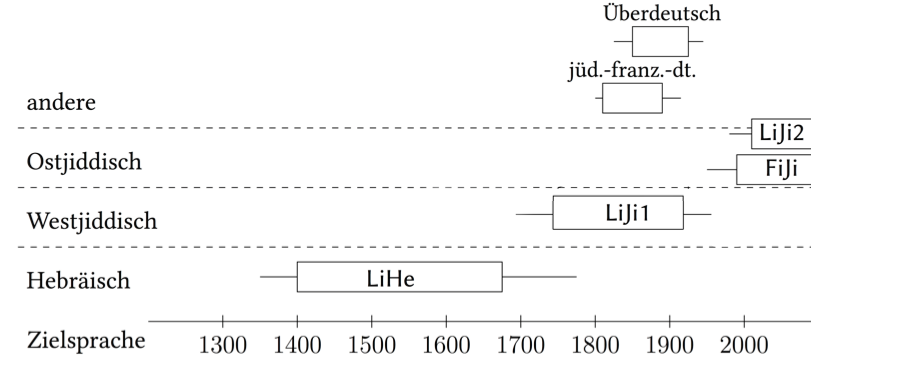
\includegraphics[width=\textwidth]{figures/stadien2.png}
		\caption{\label{stadien} Stadien jüdischer Figurenrede in der deutschsprachigen Literatur}
		\end{figure}



\noindent Wir sehen, dass die sprachliche Markierung jüdischer Rollen in der deutschsprachigen Literatur eine sehr lange Tradition hat. Wie sich die verschiedenen Rollen im Laufe der Zeit gewandelt haben und wie sich 
% dabei 
%\todo{rephrase}
mit ihnen 
die Funktionen der sprachlichen Markierung gewandelt haben, wird diese Arbeit nicht zeigen können. Mit der detaillierten Analyse des \hai{{\LiJi}1} fängt diese Arbeit zumindest einen \,%rs einen
Detailausschnitt aus dem Gesamtbild jüdischer Figurenrede und ihrer \,%rs +r
Funktionen und Formen im literarischen Diskurses zwischen 1700 und dem frühen \,%rs frühen
20. Jahrhundert ein. 



\chapter{Der Nutzen des Literaturjiddischen für die Sprachwissenschaft}\label{lijisprachwissenschaft}

%\epigraph{\begin{flushright}\RL{מיר ווייסן צו ווינציק וועגן מער{ב\makebox(-0.8,9)[r]{\libertineGlyph{uni207B}}}דיקן {{יי}\makebox(-1.5,-5.5)[r]{\libertineGlyph{afii57807}}}דיש, א\makebox(-1.5,-7.5)[r]{\libertineGlyph{uni207B}}ז מיר ז{א\makebox(-1.25,-1.25)[r]{\libertineGlyph{uni05B8}}}לן קענען מוותּר ז{יי}\makebox(-1.5,-7.5)[r]{\libertineGlyph{uni207B}}ן א\makebox(-1.5,-7.5)[r]{\libertineGlyph{uni207B}}פֿילו אויף א\makebox(-1.5,-7.5)[r]{\libertineGlyph{uni207B}} ברעקל עווידענץ.}\end{flushright}%LS! als Zitat einbinden 

%\scriptsize{\sem{Wir wissen zu wenig vom Westjiddischen, als dass wir selbst auf ein Stückchen Evidenz verzichten könnten.}}}{--- \textup{\cite[63]{Weinreich1953}}}

\noindent In seinem Übersichtsartikel zu Forschungsstand und Quellenlage des Westjiddischen geht \cite[62--63]{Weinreich1953} ausdrücklich auf literarische Texte nicht-jüdischer Autoren\footnote{\cite[62]{Weinreich1953} schreibt \quji{\RL{די ד{יי}\makebox(-1.5,-2.5)[r]{\libertineGlyph{uni207B}}טשן}} \sem{die Deutschen}, worunter selbstverständlich auch deutsche Juden fallen würden, jedoch zählt er nur Beispiele christlicher Autoren auf und nennt hingegen in den davorstehenden \,%rs ein Wort
Abschnitten (v.a. \citealt[40–42, 46]{Weinreich1953}) literarische Texte jüdischer Autoren als weitere potenzielle Quellen, woraus sich schließen lässt, dass er an dieser Stelle ausschließlich auf die nicht-jüdische Bevölkerung Deutschlands referiert.} als eine potenzielle Quelle zum Westjiddischen ein und betont deren Nutzen zur Gewinnung historischer Sprachdaten. Exemplarisch nennt er die Publikationen Itzig Veitel Sterns (Pseudonym) und das Drama \qu{Unser Verkehr} (1816) von Karl Borromäus Sessa. \citeauthor{Weinreich1953} sieht zwar, dass eine ernsthafte Analyse dieser Texte absurd wirkt, betont aber, dass im Fall des Westjiddischen jede noch so abwegige Quelle wichtig ist:

\begin{quote}
{\begin{flushright}\RL{א\makebox(-1.5,-7.5)[r]{\libertineGlyph{uni207B}}ז עס איז \RL{{פ\makebox(-0.8,8)[r]{\libertineGlyph{uni207B}}}}א\makebox(-1.5,-7.5)[r]{\libertineGlyph{uni207B}}רא\makebox(-1.5,-7.5)[r]{\libertineGlyph{uni207B}}ן נ{א\makebox(-1.25,-1.25)[r]{\libertineGlyph{uni05B8}}}ך א\makebox(-1.5,-7.5)[r]{\libertineGlyph{uni207B}} \RL{{פ\makebox(-0.8,9)[r]{\libertineGlyph{uni207B}}}}{א\makebox(-1.25,-1.25)[r]{\libertineGlyph{uni05B8}}}נד מקורים וועגן מער{ב\makebox(-0.8,9)[r]{\libertineGlyph{uni207B}}}דיקן {{יי}\makebox(-1.5,-5.5)[r]{\libertineGlyph{afii57807}}}דיש, וו{א\makebox(-1.25,-1.25)[r]{\libertineGlyph{uni05B8}}}ס כ{א\makebox(-1.25,-1.25)[r]{\libertineGlyph{uni05B8}}}טש אונדזער ערשטע רעא\makebox(-1.5,-7.5)[r]{\libertineGlyph{uni207B}}קציע איז \quji{מוקצה}, קענען מיר זיך \RL{{פ\makebox(-0.8,9)[r]{\libertineGlyph{uni207B}}}}{א\makebox(-1.25,-1.25)[r]{\libertineGlyph{uni05B8}}}רט דער\RL{{פ\makebox(-0.8,8)[r]{\libertineGlyph{uni207B}}}}ון ניט {א\makebox(-1.25,-1.25)[r]{\libertineGlyph{uni05B8}}}{פ\makebox(-1,4)[r]{\libertineGlyph{afii57807}}}ז{א\makebox(-1.25,-1.25)[r]{\libertineGlyph{uni05B8}}}גן.}  \end{flushright}}


{\begin{flushright}\LR{\cite[62]{Weinreich1953}}  \end{flushright}}
{\LR{\textit{\footnotesize{az es is faran nokh a fond mekoyrem vegn meyrevdikn yidish, vos khotsh undzer ershte reaktsie iz \qu{muktse}, kenen mir zikh fort derfun nit opzogn.}} }}\\
\LR{\footnotesize{\sem{Es gibt noch weitere Quellen zum Westjiddischen, zu denen zwar unsere erste Reaktion \qu{unbrauchbar} ist, von denen wir uns aber nicht lossagen können.}}} 
\end{quote}



 Der primäre Nutzen einer gezielten und umfangreichen Untersuchung literaturjiddischer Texte nicht-jüdischer Autoren liegt darin zu prüfen, wie geeignet diese als Quellen  des Westjiddischen sind und was sie uns über das Westjiddische und dessen Sprachsituation verraten können.

Doch Weinreichs \isi{Artikel} zur westjiddischen Forschungsagenda bleibt, trotz doppeltem Abdruck, lange Zeit unberücksichtigt. \cite{Althaus1981} ist die einzige Arbeit zur jüdischen Figurensprache mit einem linguistisch-jiddistischen Hintergrund. Obzwar dieser darin autochthone jiddische Strukturen aufzeigt, kommt er zu dem Schluss, dass es sich dabei lediglich um pervertiertes Jiddisch handelt. \cite{Weinreich1953} wird keine Beachtung geschenkt. Die literaturwissenschaftliche Arbeit Richters (\citeyear[insbes.\,99–113]{Richter1995}) äußert die Vermutung, dass die Formen des Literaturjiddischen nicht bloß der Phantasie der Autoren geschuldet sind, sondern tatsächliche Sprachrealitäten abbilden. 

Jedoch sind die Arbeiten von  \cite{Althaus1981} und \cite{Richter1995}\footnote{\citeauthor{Richter1995} analysiert immerhin elf Quellen gründlich, darunter auch das von \cite[62]{Weinreich1953} angeführte Theaterstück \qu{Unser Verkehr} (1816), jedoch steht bei ihm die literaturwissenschaftliche Analyse im Vordergrund.} auf eine nur sehr kleine Auswahl an Texten beschränkt. Auch steht die sprachwissenschaftliche Analyse nicht im Zentrum dieser Untersuchungen. Hinzu kommt, dass in den vergangenen Jahren erste Arbeiten erschienen sind, die den Versuch unternehmen, das Westjiddische des (langen) 19. Jahrhunderts aus den überlieferten Resten heraus zu rekonstruieren \citep{AptrootGruschka2004,Reershemius2007,Reershemius2014,Schaefer2008,Schaefer2010,Schaefer2013,Schaefer2014,Weisskirchen2011,FleischerSchaefer2012}. Damit ist es erstmals möglich, einen Vergleich zwischen Quellen jüdischer und nicht-jüdischer Autoren anzustellen.


\section{Natürliche, konstruierte und fiktionale Sprachen}\label{kunstsprachen}
 \largerpage %longdistance
Um das Verhältnis zwischen \ili{Literaturjiddisch} und gesprochenem \ili{Westjiddisch} zu verstehen, muss man sich der Verhältnisse zwischen fiktionalen, natürlichen und konstruierten Sprachen bewusst werden. Der Begriff \quein{fiktionale Sprache} steht hier entsprechend dem englischen \quein{fictional language} für Sprachen, die ausschließlich innerhalb eines künstlichen Mediums (Literatur, Film) realisiert sind. Mit dieser medialen Fixiertheit unterscheiden sich fiktionale Sprachen von \quein{natürlichen Sprachen}, die sich dadurch auszeichnen, dass sie muttersprachlich erworben werden (\hai{L1}; \hai{N1}-Sprachen in der Diktion von  \citealt[90]{Weiss2001}) und das Potenzial zur Variabilität haben.\footnote{D.\,h. strukturelle Viskosität gegeben ist, vgl.\, S.\, \pageref{viskoserstemal}.} Fiktionale Sprachen sind ein Untertyp von \quein{konstruierten Sprachen}. Konstruierte Sprachen haben die Eigenschaft, dass sie nur als Zweitsprache (\hai{L2}; \hai{N2}-Sprachen nach \citealt[90]{Weiss2001}) erworben werden können, nur beschränkte Variabilität besitzen (und keine viskosen Strukturen haben, s.u.). Zu ihnen zählen formale Sprachen wie Programmiersprachen, aber auch Sprachkonzepte bzw. Metasprachen, die in Grammatiken und Regelwerken festgelegt sind, oder Plan-, Geheim- und Sondersprachen. Da Standardsprachen überwiegend präskriptive Sprachkonzepte sind und auch nie den Gesamtumfang einer natürlichen Sprache erfassen können, fallen sie ebenfalls in die Kategorie formaler, konstruierter Sprachen (vgl.\, \citealt[51]{Chomsky1995}). Das Regelwerk konstruierter Sprachen kann naturalisiert werden, sofern ihre Regeln aktiv angewandt werden und an Kinder als Erstsprache weitergegeben werden, die diese Regeln kreolisieren, wie man es besonders deutlich bei Plan-, Geheim-, Sonder- und Standardsprachen sieht. Eine direkte Beeinflussung fiktionaler Sprachen durch natürliche Sprachen ist z.\,B.\, im Fall des Khuzdul, der Sprache der Zwerge in Tolkiens  \qu{The Hobbit or There and Back Again} (1937) und \qu{The Lord of the Rings} (1954/1955), gegeben, welches sich an semitischen Sprachen (insbes. dem biblischen Hebräischen) orientiert (vgl.\, \citealt[120]{ConleyCain2006}). Eine fiktionale Sprache kann auch den Status einer natürlichen Sprache erlangen. Ein bekanntes Beispiel für den Versuch, aus einer fiktionalen Sprache eine natürliche Sprache zu generieren, sind die bislang gescheiterten Naturalisierungsversuche des Klingonischen der Science-Fiction Reihe \qu{Star Trek} (vgl.\, \citealt{Okrent2010}). Damit  eine fiktionale Sprache sich zu einer natürlichen Sprache entwickeln kann, muss diese jedoch zunächst reglementiert werden. Die meisten fiktionalen Sprachen unterscheiden sich von den übrigen Subtypen konstruierter Sprachen darin, dass sie ursprünglich nicht auf metasprachlich erfassten Regeln beruhen, was in ihrer fiktionalen Funktion begründet ist: Fiktionale Sprache beschränkt sich i.\,d.\,R. auf die Zeichenhaftigkeit selbst. Inhalts- und Ausdrucksseite sind dabei peripher und werden zumeist von der natürlichen Sprache des Mediums etwa durch Übersetzungen oder Untertitel übernommen.

 \largerpage %longdistance
Konstruierte und natürliche Sprachen beeinflussen sich gegenseitig. Exemplarisch lassen sich die ablaufenden Prozesse in den Entwicklungen des Aramäischen nachvollziehen: Zu den Zeiten der Abfassung von Tanach und Talmud waren \ili{hebräisch}-aramäische Varietäten natürliche Sprachen. Durch die jüdische Mehrsprachigkeit der Diaspora verliert das Aramäische an Muttersprachlern, bleibt konserviert als Sakralsprache und entwickelt sich mehr und mehr zu einer konstruierten Sprache, die zwar immer noch als \hai{L2}-Sprache erworben wird, jedoch in der Regel keinen aktiven Gebraucht hat. In manchen Fällen erlangt Hebräisch in der jüdischen Kultur des späten Mittelalters und der frühen Neuzeit sogar den Status einer fiktionalen Sprache, die nur noch innerhalb der Literatur eine Realität besitzt, sprich die Sprache literarisch konserviert ist. Im Zuge des Zionismus des 19. und 20. Jahrhunderts wird mit dem modernen Ivrit eine konstruierte Varietät des Hebräischen entwickelt, die über einen durch politische Umstände geschaffenen muttersprachlichen Erwerb renaturalisiert wurde. Der Theorie Zuckermann (u.\,a.\, \citeyear{Zuckermann2004,Zuckermann2006}) folgend hat jedoch erst der Einfluss natürlicher Sprachen (insbes. des Jiddischen) zur Revitalisierung des Hebräischen im Ivrit als eine fussional-synthetische Sprache beigetragen. Eine Naturalisierung fiktionaler Sprache ist ohne eine rahmenbildende natürliche Sprache nicht möglich.

Für das Literaturjiddische als fiktionale Sprache bleibt zunächst zu klären, ob es sich dabei entweder um ein reines Phantasieprodukt handelt oder ob es auf einer (oder mehreren) natürlichen Sprache(n) beruht. Diese natürliche Sprache wäre idealerweise das Westjiddische, sie kann aber auch ein \qu{intuitives und literarisches Kreolisieren} (\citealt[135]{Haider2007}) des Deutschen, als der Muttersprache nicht-jüdischer Autoren, sein. Mit der emulierenden \isi{Imitation} als Strategie zur Bildung fiktionaler Sprache haben wir es mit einem Sonderfall zu tun. Die daraus resultierenden Medialekte sind eingebunden in eine natürliche Sprache (Matrixsprache). Die Ausdifferenzierung, wo die \isi{Imitation} einsetzt und wo sie aufhört, ist in vielen Fällen problematisch, da hier konstruierte und natürliche Sprache ineinander greifen. Es können daher nur jene Formen als Produkt der Fiktionalisierung gewertet werden, die sich strukturell eindeutig von der Matrixsprache distanzieren. 

\section{Imitation als Feld für psycho- und variationslinguistische Fragestellungen}\label{salienz}
 
Gesetzt den Fall, dass sich die deutschsprachigen Autoren in der Entwickeln des Literaturjiddischen an der tatsächlichen Sprachrealität des Jiddischen orientierten, so lägen uns mit einem \isi{Korpus} dieser fiktionalen Sprache historische Imitationsdaten vor. Ein Quelltyp, der bislang in der Sprachgeschichtsforschung keine Rolle gespielt hat. Bei der \isi{Imitation} rufen Autoren ihre Laienkonzepte des Jiddischen ab. Diese Laienkonzepte können zum einen ihren Ursprung im direkten \isi{Sprachkontakt} zum Jiddischen haben, zum anderen aber auch durch den internen Diskurs um das Jiddische in der deutschsprachigen Literatur und Kultur angeregt und verfestigt worden sein (vgl.\, \citealt[98f]{Richter1995}).   

Doch selbst wenn man davon ausgeht, dass \ili{Literaturjiddisch} in keinem direkten Bezug zum Jiddischen steht, sondern rein konstruiertes Produkt von Muttersprachlern des Deutschen ist, ein \quein{dekonstruiertes Deutsch}, so dürfen wir annehmen, dass diese Sprache den Grundstrukturen germanischer Sprachen unterworfen ist, sofern die Autoren nicht über exzellente Sprachkompetenzen in nicht-germanischen Sprachen verfügen, die sie einfließen lassen. So zeigt Haider (\citeyear{Haider2007}) am Beispiel von Jandls \quein{heruntergekommener Sprache}, dass eine fiktionale Sprache auf Basis des Deutschen vollständig dem entsprechen kann, was in germanischen Sprachen und Kreolisierungen germanischer Sprachen möglich ist. Über emulierende Sprachimitationen können wir damit nicht nur etwas über die zu imitierende Sprache (Zielsprache) lernen, sondern sie zeigen uns vor allem die Möglichkeiten der Matrixsprache (Ausgangssprache).\label{viskoserstemal}

An dieser Stelle möchte ich den Begriff der sprachlichen \quein{Viskosität} einführen, der die potenzielle Flexibilität eines sprachlichen Systems bezeichnet. Je höher die sprachliche Viskosität einer Struktur ist, umso geringer ist ihre Flexibilität, d.\,h. Variabilität. Um ein Beispiel zu nennen, sind etwa germanische \hai{OV}-Sprachen verbsyntaktisch durch eine niedrigere Viskosität gekennzeichnet als germanische \hai{VO}-Sprachen, da erstere deutlich mehr Variation bezüglich der Verbserialisierung aufweisen als letztere (vgl.\, Abschnitt \ref{verbsyntax}, S.\, \pageref{verbsyntax}). Die Positionen, in denen ein sprachliches System besonders geringe Viskosität aufweist, können besonders leicht in emulierenden Imitationen manipuliert werden, ohne starke Verletzungen am System der Matrixsprache vorzunehmen. Hierfür ist der Begriff der \quein{Manipulation} zentral: Die Viskosität eines Systems (\textit{I-Language}) 
bestimmt, wie stark/schwach mögliche Eingriffe (Manipulationen) in das jeweilige System sind. Für das Beispiel der Verbserialisierung heißt dies, dass Abfolgevariationen innerhalb des Verbgefüges in germanischen \hai{OV}-Sprachen mit einer höheren Wahrscheinlichkeit im Bereich der emulierenden \isi{Imitation} manipuliert werden als in \hai{VO}-Sprachen. Dies muss zunächst einmal nicht daran geknüpft sein, wie die Strukturen der Zielsprache tatsächlich aussehen. Die Viskosität einzelner Strukturbereiche einer Sprache können uns auch einen Einblick darin geben, wie und wo Sprachwandel greift bzw. nicht greift. Doch dies ist nur ein Aspekt unter vielen, für den sich die Untersuchung sprachlicher Imitationen als gewinnbringend erweist. 

\isi{Imitation} kann nur stattfinden, wenn eine zu imitierende Sprache bekannt ist (etwa durch direkten oder indirekten \isi{Sprachkontakt}). Da wir den christlichen Autoren des 19. Jahrhunderts eine Kompetenz des Jiddischen weitestgehend absprechen,\footnote{Es mag einzelne Ausnahmen gegeben haben, bei denen eine Teilkompetenz anzunehmen ist, wie etwa die Sondersprachen Lachoudisch im fränkischen Schopfloch (\citealt{Hofmann1998,Klepsch1996,Klepsch2004,Klepsch2008,Matras1996,Philipp1983}) oder Lotegorisch in der Pfalz (\citealt{Meissner1999}) zeigen. Vor allem unter dem Bildungsbürgertum (zumeist Theologen), aber auch unter Händlern nahmen seit dem 16. Jahrhundert die Bestrebungen, Jiddisch zu erlernen, zu (\citealt{Elyada2012}). Wie weit dies jedoch die deutschsprachige Durchschnittsbevölkerung betraf und wie kompetent Christen tatsächlich in der jiddischen Sprache waren, ist schwer zu ermitteln. Für die Literaten des 19. Jahrhunderts kann zwar angenommen werden, dass sie einige Grammatiken der Hebraisten zur Kenntnis genommen haben, die wenigsten unter diesen bieten jedoch eine Basis zum Erlernen des Jiddischen, da i.\,d.\,R. lediglich Hebraismen aufgelistet werden und nur in Ausnahmefällen (z.\,B.\, \citealt{Haselbauer1742,Friedrich1784}) einzelne Beispielsätze angeführt sind. Von modernen Grammatiken zum Zweitspracherwerb sind diese Arbeiten sehr weit entfernt. Bei Konvertiten (\textit{Judenchristen}) sind natürlich Kompetenzen im Jiddischen anzunehmen.} kann angenommen werden, dass die Grundprinzipien der deutschen Grammatik den äußeren Rahmen dieser fiktionalen Sprache bestimmt haben. Hinter der Grundidee der sprachlichen \isi{Emulation} steht auch die Überlegung, dass die Autoren das Jiddische nicht als eigenständige Sprache verstanden haben, sondern es immer im direkten Bezug zum Deutschen wahrnahmen, ähnlich einem deutschen Dialekt (vgl.\, \citealt[127–136]{Elyada2012}). Laienkonzepte werden innerhalb des deutschen Systems emuliert, d.\,h. fremde Strukturen werden an das bestehende System angepasst. Die deutsche Sprache wird manipuliert, um den Effekt des Jiddischen zu erreichen. Die einzelnen Strukturen der Manipulation können uns Aufschluss darüber geben, wie die Laienkonzepte des Jiddischen aussahen, welche wiederum bis zu einem gewissen Grad auch auf die Sprachrealität verweisen.  

Kontaktinduzierte Interferenzen erfassen in erster Linie Strukturen, die vom Basissystem verarbeitet werden können. Demgegenüber nehmen Strukturen weniger Einfluss auf diese Form von Sprachwandel, die auffällig, komplementär anders, \textit{bewusst wahrnehmbar}, im dialektologischen Sinne \textit{salient} sind. Im Fall der Imitation des Jiddischen dienen die sprachlichen Strukturen der Sprachstatik, weil sie das \textit{Eigene} vom \textit{Fremden} bewusst abgrenzen (vgl.\, \citealt[70]{Guenthner2002}). Dies steht komplementär zu den in der Variationslinguistik gängigen Grundüberlegungen vom Zusammenspiel von \quein{Salienz} und \quein{Sprachwandel}, wie sie seit Schirmunskis (\citeyear[118]{Schirmunski1930}) vielmeinenden Ausspruchs die Dialektologie beschäftigen (vgl.\, u.\,a.\, \citealt{HerrgenSchmidt1985,Lenz2010,Elmentaleretal2010,Purschke2011,Purschke2014,Kiesewalter2011,Kiesewalter2014,Hettler2014,Auer2014,Glauninger2014,AndersPalliwodaSchroeder2014,Lorenz2014}): 


\begin{quote}
Wir bezeichnen im weiteren die charakteristischen, d.h. am stärksten auffallenden Abweichungen einer Mundart gegenüber der Schriftsprache (oder anderen Mundarten) als primäre Merkmale, die weniger auffallenden Abweichungen als sekundäre Merkmale. (\citealt[118]{Schirmunski1930})
\end{quote}


Die in dieser Arbeit verwendete Definition von \quein{Salienz} orientiert sich nicht an der dialektologischen Verwendung, die unter \textit{salienten Merkmalen} in der Regel signifikante Merkmale versteht, die bewusst sind. Hingegen bedient sich diese Arbeit eines Salienzbegriffs, wie er u.\,a.\, in Psychologie, Neurologie oder Soziologie üblich ist: Hier bezeichnet \isi{Salienz} die allgemeine Wahrnehmung eines Reizes gegenüber anderen Reizen. Die Wahrnehmung muss dabei nicht auf bewusster Ebene erfolgen, sondern Strukturen  müssen salient sein um bewusst zu werden, d.\,h. wahrnehmbar sein, um bewusst zu werden. Damit eine Struktur bewusst wahrgenommen wird, ist jedoch die Grundvorraussetzung ihre \isi{Salienz}, was jedoch nicht impliziert, dass jede saliente Struktur bewusst wird. Welches sprachliche Merkmal \isi{Salienz} auslöst, ist abhängig vom Grad der typologischen Distanz und Viskosität der Matrixsprache (Ausgangssprache) zur Kontaktsprache und von Grad und Intensität des Sprachkontakts. Nur saliente Strukturen, die verarbeitet werden, können in das System der Matrixsprache aufgenommen werden und dort durch \isi{Emulation} Sprachwandel hervorrufen. Im Rahmen des hier verwendeten Imitationsbegriffs bezeichnet \isi{Salienz} die neuro-kognitive Ebene des \quein{Filters}, der zwischen Zielsprache und Matrixsprache besteht (vgl.\, Abschnitt \ref{begriffsdefinitionen}, S.\, \pageref{emulationsbegriff}). Bewusst wahrgenommene Strukturen können immer nur auf einer Metaebene wirken. Sprachwandel hingegen betrifft das System selbst. Daher kann natürlicher Sprachwandel, d.\,h. Sprachwandel, der nicht durch eine bewusste Sprachlenkung, wie etwa Standardisierung oder Zweitspracherwerb beeinflusst ist, nur bedingt auf salienten Merkmalen aufbauen. Viel wichtiger sind Strukturen, die vom sprachlichen System selbst verarbeitet werden können. Natürlicher Sprachwandel ist in dem Sinne eine Modifizierung des sprachlichen Systems. Die menschliche Fähigkeit zur \isi{Imitation} spiegelt diese Möglichkeit zur Modifikation wider. \isi{Imitation} ist damit nicht ohne Grund der Ausgangspunkt des kindlichen Spracherwerbs (vgl.\, u.\,a.\, \citealt{Uzgiris1981}; \citealt[291–294]{Tauten1997}). Die Imitationsdaten des Literaturjiddischen bieten einen Einblick in diese Strukturen des Sprachkontakts zweier nahverwandter Varietäten. 

Erst die strukturelle Analyse der jüdischen Figurenrede kann die Frage klären, ob es ein allen Texten gemeinsames Konzept vom Literaturjiddischen gab, oder ob jeder Autor seine eigene fiktionale Sprache entwickelte. %Im Fall, dass die Analyse (Abschnitt \ref{analysen}) erstere Annahme bestätigt.\,%rs hier fehlt das weiterführende!
Im Fall eines einheitlichen Literaturjiddischen kann die Vermutung aufgestellt werden, dass Laienkonzepte auf einer einheitlichen Wahrnehmung und Reproduktion sprachlicher Formen natürlicher Sprache fußen. Zugleich spräche dies aber auch dafür, den innerliterarischen Diskurs als Katalysator literaturjiddischer Formen zu verstehen. Würde jeder Autor andere Formen der sprachlichen Markierung verwenden, so ließe sich der literarische Diskurs als Triebfeder ausschließen und erst der Vergleich zu autochthon westjiddischen Quellen kann entscheiden, ob der Autor auf ein Laienkonzept oder seine Phantasie zurückgreift. Ein interessantes Ergebnis wäre, wenn sich das Literaturjiddische regional und nicht idiolektal unterscheiden würde. So ließe sich zum einen darauf schließen, dass die Autoren ihre eigene Dialektalität, sprich dialektales Deutsch, haben einfließen lassen oder aber sogar, dass die westjiddischen Varietäten im Raum streuen und wir somit erstmals dialektale Strukturen erkennen könnten.

  
Das Einfließen deutsch-dialektaler Strukturen in das Literaturjiddische wiederum führt uns in den Bereich der Diglossieforschung (vgl.\, \citealt{Ferguson1959}). Gerade für das 18. und 19. Jahrhundert kann man davon ausgehen, dass die meisten Autoren in einer diglossischen Sprachsituation zwischen Schriftsprache und gesprochener Sprache (Dialekt) standen. Eine Diskrepanz zwischen Schriftlichkeit und Mündlichkeit findet sich bis in die heutige Zeit (vgl.\, \citealt{KochOesterreicher1985}), mit dem Unterschied, dass nun kaum mehr (Basis-)Dialekte, sondern Regiolekte und nicht-arealgebundene Soziolekte die Mündlichkeit ausmachen (vgl.\, \citealt{SchmidtHerrgen2011}). So ist anzunehmen, dass bei dem Versuch, (jiddische) Dialektalität in die literarische Schriftlichkeit zu transponieren, die eigene Umgangssprache einfließt. Aus diesem Grund wird die nachfolgende Analyse auch immer die gewonnenen Daten des Literaturjiddischen mit der Situation in den deutschen Dialekten abgleichen (s. Abschnitt \ref{analysen}). Darüber hinaus funktioniert der Einsatz des Literaturjiddischen ähnlich wie \quein{code-mixing} (vgl.\, \citealt{MyersScotton2004,MyersScotton2002}): jüdische Figuren \textit{sprechen} ein Schriftdeutsch, welches durchsetzt ist mit jiddischen bzw. mit als \quein{jiddisch} verstandenen Elementen.  

Emulierende fiktionale Sprachen wie das \hai{{\LiJi}} können uns darüber hinaus dabei helfen, den kognitiven Aufwand von sprachlicher Rekonstruktion nachzuvollziehen. 
Der Umstand, dass nur bestimmte Formen emuliert werden, ist nicht zwangsläufig autochthonen jiddischen Formen geschuldet, sondern gibt auch Hinweise auf die Struktur unserer Sprachverarbeitung. Dies möchte ich an einem Fallbeispiel illustrieren: Will ein Autor eine jüdische Figur jiddisch sprechen lassen und möchte zusätzlich, dass der Inhalt der Figurenrede für die Leserschaft verständlich ist, hätte er vier Möglichkeiten: 

\begin{itemize}
\item [1.] Verwendung des Jiddischen (erworben durch Grammatiken, Kontakt mit Muttersprachlern o.\,ä.).
\item [2.] Verwendung des Jiddischen (erworben durch Grammatiken, Muttersprachler o.\,ä.) mit paralleler Übersetzung in die Matrixsprache (Deutsch).
\item [3.] Verwendung des Deutschen mit Elementen des Jiddischen (aus eigenem Laienkonzept, welches auf direktem \isi{Sprachkontakt} beruht).
\item [4.] Verwendung des Deutschen mit Elementen des \hai{{\LiJi}} (sofern kein Laienkonzept aus direktem \isi{Sprachkontakt} vorhanden ist).
\end{itemize}

Nur in den Fällen 2, 3 und 4 wäre eine Verständlichkeit des Sprechtexts der jüdischen Figur durch den Leser garantiert. Möglichkeit 1 kann damit ausgeschlossen werden. Da es wohl ein zu hoher Aufwand für einen Autor wäre, sich die jiddische Sprache anzueignen und v.\,a.\, da eine Übersetzung den Lesefluss beeinträchtigen würde, sind keine Texte zu finden, die sich Möglichkeit 2 zunutze machen. Bei den verbliebenen Strategien 3 und 4 ist die Verständlichkeit garantiert, solange emulierte Formen in die Matrixsprache (Deutsch)  rekonstruiert werden können. Dabei muss der Autor/Leser des \hai{{\LiJi}} über die kognitive Fähigkeit verfügen, zu wissen, welche sprachlichen Strukturen sich rekonstruieren bzw. nicht mehr rekonstruieren lassen. Anhand von emulierenden fiktionalen Sprachen ließe sich testen, welche sprachlichen Strukturen höherer Verarbeitungsleistungen bedürfen als andere. Die aus dem \hai{{\LiJi}} gewonnenen Daten könnten so als Grundlage für psychoneurolinguistische Untersuchungen der Wort- und Sprachverarbeitung dienen.

Doch bereits die Formen, die wir im \hai{{\LiJi}} finden, können als positive Evidenz für leicht rekonstruierbare Strukturen interpretiert werden.

Damit bringt eine Analyse des \hai{{\LiJi}} die drei folgenden psycho- und variationslinguistischen Fragestellungen mit sich:

\begin{description}
\item [] i. Was ist in der Matrixsprache (Deutsch) möglich (= d.\,h. was ist überhaupt konstruierbar)?
\item [] ii. Was sagt dies über die typologische Beschaffenheit und Nähe von Zielsprache (Jiddisch) und Matrixsprache (Deutsch) aus?
\item [] iii. Was kann aus dem \hai{{\LiJi}} in die Matrixsprache (Deutsch) rekonstruiert werden (= d.\,h. was ist überhaupt verarbeitbar)?
\end{description} 


 
\section{Literaturjiddisch als Sekundärquelle des späten Westjiddisch}\label{secundärquelle}
 
Die in den Abschnitten \ref{kunstsprachen} und \ref{salienz} dargelegten Prämissen erlauben die Annahme, dass die Sprachrealität des Westjiddischen ihren Niederschlag im Literaturjiddischen gefunden hat. So betrachtet können die zu untersuchenden literarischen Texte als Sekundärquellen zum Jiddischen verstanden werden. Dies ließe sich im Vergleich zu unserem derzeitigen Wissen über das späte \ili{Westjiddisch} (s. Abschnitt \ref{westjiddistik}) prüfen. Für den Fall, dass die literaturjiddischen Quellen tatsächlich Nähe zum Westjiddischen aufweisen, würde dies unsere bisher gewonnenen Daten bestätigen. Darüber hinaus ließen sich aber auch Erweiterungen unseres Wissens erwarten, sofern Strukturen im Literaturjiddischen auftreten, die wir nur vereinzelt in westjiddischen Primärquellen finden. Des Weiteren lassen sich Vermutungen über die Authentizität bisher unbelegter Strukturen machen, sofern diese in den Sekundärquellen wiederholt in Erscheinung treten.

Literaturjiddische Texte können aber auch soziolinguistische Prozesse widerspiegeln. So ist anzunehmen, dass der westjiddische \isi{Sprachtod} im Rückgang westjiddischer Formen im Literaturjiddischen reflektiert wird. Demgegenüber ist ein möglicher Zugewinn ostjiddischer Formen im Verlauf des 19. Jahrhunderts parallel zum kulturellen Aufstieg dieser Sprache und möglicher Migrationsbewegungen von Ostjiddischsprechern in den Westen nicht auszuschließen.

  
\part{Datengrundlage und Methodik}\label{datengrundlage} 
\chapter{Quellen des späten Westjiddischen}\label{chap:quellenkapitel}
 % \epigraph{\textit{Historical documents survive by chance, not by design}}{--- \cite[11]{Labov2010}}
  
  \noindent Die Westjiddistik steht, da sie sich um die Erforschung einer ausgestorbenen, historischen Sprache bemüht, in Abhängigkeit zu den uns überlieferten Quellen (vgl.\, \citealt{Weinreich1953}). Die meisten Arbeiten zum späten Westjiddischen konzentrieren sich auf die Dokumentation und Beschreibung des gesprochenen, noch vitalen (West-)Jiddischen nach der Schoah. So z.\,B.\, die Atlasprojekte von \cite{GuggenheimGruenberg1973}, \cite{Beraneck1965}\footnote{\citeauthor{Beraneck1965}s \qu{Westjiddischer Sprachatlas} ist aufgrund \qu{zweifelhafte[r] Ergebnisse und methodische[r] Fehlgriffe} (\citealt[1020]{Katz1983}) als fragwürdige wissenschaftliche Leistung zu beurteilen (vgl.\, \citealt{GuggenheimGruenberg1966b,GuggenheimGruenberg1968}; \citealt[1377—1378]{Althaus1972}; \citealt[1020]{Katz1983}).} und der  von Uriel Weinreich begründete Atlas \qu{Language and Culture Atlas of Ashkenazic Jewry} (\citealt{Herzog1992} \citeyear{Herzog1992,Herzog1995,Herzog2000}; zum \hai{{\WJ}} besonders \citealt{Zuckerman1969}). Diese Arbeiten konnten jedoch nur mehr die vitalen Varietäten des Elsass, der Schweiz und von Teilen Südbadens erfassen. Generell gilt, dass der Raum des westl. \hai{{\SWJ}} besonders überrepräsentiert ist, was die Quellenlage, aber auch was die wissenschaftlichen Arbeiten betrifft \,%rs anstelle von "was… betrifft" in Hinblick auf sowohl…als auch
  (vgl.\, \citealt{Weiss1896,GuggenheimGruenberg1958,GuggenheimGruenberg1966,GuggenheimGruenberg1973,GuggenheimGruenberg1976,GuggenheimGruenberg1981,Zuckerman1969,Brosi1990,Fleischer2004,Fleischer2004b,Fleischer2005,Schaefer2008,Schaefer2014}{; }\citealt{Weisskirchen2011}). Zum \hai{{\ZWJ}} gibt es hingegen nur einige wenige lexikalische Arbeiten, die sich meist auch nur auf jiddische Lehnwörter in den deutschen Dialekten stützen (\citealt{Frank1962,Weinberg1973,Althaus1963,Post1992,Klepsch2004}). Aber nur die Arbeiten von \cite{Frank1962} (\hai{{\ZWJ}}) und \cite{Weinberg1973} (\hai{{\NWJ}}) beruhen auf Interviews mit Muttersprachlern und/oder mit der nachfolgenden Generation der letzten Sprecher des Westjiddischen. Unser Wissen zum \hai{{\NWJ}} basiert überwiegend auf Untersuchungen  literarischer Quellen (vgl.\,\citealt{Landau1901,Reershemius2007,Reershemius2014,Schaefer2013}). Zum niederländischen \hai{{\NWJ}} liegen Untersuchungen zur Lexik und Phonologie vor (\citealt{VanGinneken,VoorzangerPolak1915,Beem1954,Beem1970,Beem1974,Beem1975,Aptroot1991,Aptroot2002}). Forschungsbedarf besteht im östl. \hai{{\SWJ}} sowie in den Übergangszonen. Immerhin zum ungarischen Jiddischen liegen uns \,%rs Zum ungarischen Jiddischen liegen uns immerhin
  die Arbeiten \citeauthor{Hutterer1965}s (\citeyear{Hutterer1965,Hutterer1994}) und \citeauthor{Garvin1965}s (\citeyear{Garvin1965}) vor. Auch das \hai{{\NÜJ}} ist in \cite{Herzog1965} gut erfasst. Zum Jiddisch im \ili{tschechisch}-slowakischen Sprachgebiet sind die Arbeiten \citeauthor{Trost1965}s (\citeyear{Trost1965}) und Beraneks (\citeyear{Beranek1936,Beranek1949}) unsere einzigen Quellen. Eine Zusammenstellung der Quellen zum Burgenländer Jiddisch findet sich neben einer knappen Darstellung der sprachlichen Eigenschaften in \textcite{Schaefer2017}.

Doch birgt die Quellenlage zum Westjiddischen noch immer Analysepotential für weitere Arbeiten. So nennt \cite{Weinreich1953} eine Vielzahl literarischer Quellen jüdischer wie christlicher Autoren, die uns Auskunft über den Zustand des Westjiddischen im 18. und 19. Jahrhundert liefern können. Bereits Landaus Analyse der Memoiren der Glikl bas Judah Leib kann als erster Versuch gelten, Reflexe des umgangssprachlichen Jiddischen in einem literarischen Text nachzuweisen (\citealt{Landau1901}). Mit den Arbeiten von \cite{AptrootGruschka2004}, Reershemius (\citeyear{Reershemius2007,Reershemius2014}), \cite{Weisskirchen2011}, \cite{FleischerSchaefer2012} und \citeauthor{Schaefer2008} (\citeyear{Schaefer2008,Schaefer2010,Schaefer2013,Schaefer2014}) mehren sich in jüngster Zeit Analysen des Westjiddischen, die auf literarischen Quellen des 19. Jahrhunderts fußen und damit erstmals den Sprachstand jener Zeit erfassen.

Diesem Trend folgt auch das von der Deutschen Forschungsgemeinschaft geförderte Projekt \qu{\ili{Westjiddisch} im (langen) 19. Jahrhundert: Quellenlage, soziolinguistische Situation und grammatische Phänomene} an der Philipps-Universität Marburg. In diesem Projekt wurde zwischen 2011 und 2016 in erster Linie daran gearbeitet, einen Gesamtüberblick der Quellenlage zu gewinnen. Daran anschließend werden einzelne, besonders ergiebige Quellen betreffs ausgewählter sprachlicher Phänomene analysiert und beschrieben (\citealt{Weisskirchen2011,Schaefer2013,Schaefer2014}{; }\citealt{FleischerSchaefer2012}). Die nachfolgenden Abschnitte beruhen auf dem in diesem Projekt erarbeiteten Quellsample und auf ersten daraus gewonnenen Ergebnissen.\footnote{Der dieser Arbeit zu Grunde liegende Stand des Projektsamples ist der vom 03. Oktober 2013. Eine regelmäßig aktualisierte Version des Projektsamples ist unter \url{http://www.online.uni-marburg.de/westjiddisch/} einsehbar und durchsuchbar. Die folgenden Histogramme erfassen 276 Quellen, da zu dreien kein Erscheinungsdatum eruiert werden konnte. Die Erschließung von Quellen erfolgt im Projekt über Recherchen in Judaica-Beständen von Bibliotheken und gezielte Suchabfragen in digitalen Beständen durchsuchbarer Textzeugen des (langen) 19. Jahrhunderts. Die Erfüllung/Nichterfüllung sprachlicher Charakteristika des Westjiddischen (z.\,B.\, Kennwörter wie \textit{Ette} \sem{Vater}, \textit{Memme} \sem{Mutter} oder vokalische Strukturen wie {\mhd} \textit{ei}/\textit{ou} als <aa>) entschieden dabei über die Aufnahme von Texten in das Projektsample.}

 
 
 
 
 \section{Der jüdische Multilingualismus}\label{multilingualismus}%LS dieses Kapitel habe ich etwas umgeschrieben
%\noindent
Die jüdischen Kulturen der Diaspora bewegen sich in einem Spannungsfeld  zwischen zwischen As­si­mi­la­ti­on an die jeweiligen koterritorialen Kulturen und der Bewahrung der eigenen kulturellen Identität (Dis­si­mi­la­ti­on). Diese Problematik spiegelt sich auch in den jüdischen Sprachen wieder. Das Judentum der Diaspora hat allein aufgrund der Dichotomie zwischen Alltags- und Sakralsprache immer eine bi- bzw. multilinguale Ausrichtung (vgl.\, \citealt{Weinreich1962,Mieses1915,Fischer1936}). Die Alltagssprache, insbesondere die der innerjüdischen Kommunikation, ist das Jiddische. Darüber hinaus kann man beim aschkenasischen Judentum einen Bidialektalismus nicht-jüdischer Dialekte (d.\,h. gesprochensprachlicher Varietäten) feststellen (\citealt{Weinreich1962,Schaefer2008,Schaefer2014}{; } s.\,a. \qu{Die Hochzeit zu Grobsdorf} 1822:\,2–7 in \citealt{Lowenstein1975}). Dies gilt sowohl für den ost- als auch für den westjiddischen Sprachraum. Im westjiddischen Gebiet ist zudem in der Schriftlichkeit eine Ausrichtung an deutschen Literatursprachen zu verzeichnen, die auf schriftdeutsche Varietäten der jüdischen Bevölkerung hinweisen. Der Unterschied zwischen dem Deutsch von Juden und dem von Christen darf als äußerst gering eingeschätzt werden. In der Regel handelt es sich lediglich um eine orthographische Differenz zwischen jüdischem und christlichem Schriftdeutsch (Stichwort: \sem{Deutsch in hebräischen Lettern} s. nachfolgendes Kapitel \ref{Überlieferungsformen}). In Anlehnung an Haïm Vidal Séphiha  (\citeyear[193]{Sephiha1985}) und Paul Wexler (\citeyear[7]{Wexler1987}) bezeichne ich diese Varietäten als Judeo-X-Sprachen.
Ich unterscheide jedoch zwischen zwei Typen von Judeo-X-Sprachen. Typ 1 der Judeo-X-Sprachen zeichnet sich dadurch aus, dass hier keine von der X-Sprache eigenständigen grammatischen Strukturen vorliegen und sich die Judeo-X-Sprachen lediglich auf Basis von kulturell bedingten Lexemen, welche zumeist aus der \ili{hebräisch}-aramäischen Komponente stammen, von der koterritorialen X-Sprache unterscheiden. Im Typ 2 hingegen bestehen eigenständige grammatische Strukturen der Judeo-Sprache gegenüber der X-Sprache, wie dies im Jiddischen der Fall ist. Ein weiterer Typ jüdischer Varietäten sind die auf hebräischer Lexik (und z.\,T. \isi{Morphologie}), aber auf germanischer \isi{Syntax} basierenden Sondersprachen, die auch koterritoriale Sondersprachen (insbes. rotwelsche Sprachen) beeinflusst haben (vgl.\, \citealt{GuggenheimGruenberg1981,Matras1996}).

Das nachfolgende Schema zeigt den jüdischen Multilingualismus, der sich auf einer Skala zwischen koterritorialer Kultursprache (\isi{Assimilation}) und jüdischer Sakralsprache (Dissimilation) verteilt.\footnote{Für die tatsächliche Sprachrealität ist allerdings anzunehmen, dass nur in seltenen Einzelfällen ein Individuum alle fünf Varietäten beherrscht hat.} %Besonders die Varietäten \hai{A.} und \hai{D.} sind in der jüdischen Diaspora eher selten zu finden. 


 
 \begin{description}\label{schämamultilingualismus}
  
  \item [\isi{Assimilation}/X-Sprachen]
  
  \item [A] Koterritoriale Varietäten

  \item [B] Judeo-X-Sprachen; vgl.\, \citet[193]{Sephiha1985}
  
\begin{itemize}
\item [\hai{Typ 1}] ohne von X-Sprache losgelöster Grammatik, lexikalisch markiert,\\ z.\,B.\, \textit{Judeo-Englisch}, \textit{Judeo-German}\footnote{Für den deutschsprachigen Raum ließe sich vom Judeo-German bzw. vom problematischen, weil anderweitig besetzten Terminus \textit{Jüdisch-Deutsch} sprechen (vgl.\, \citealt{FleischerimErsch}).} %format! prüfen: passt die FN hier?
\item [\hai{Typ 2}] mit von X-Sprache losgelöster Grammatik,\\ z.\,B.\, \textit{Karaimisch} (Trakei), \textit{\alert{Jiddisch}}

\end{itemize}  
 
\item [C] Hebraeo-X–Sprachen\\
 Sonder- oder Geheimsprachen,
 z.B. Händlersprachen

\item [D] Hebräisch-aramäische Varietäten\\
z.\,B.\, \textit{Ivrit}

\item[Dissimilation/Sakralsprache]

  \end{description}%AA


Dieser kurze Blick auf die jüdische Sprachsituation der Diaspora macht zweierlei deutlich: Zum einen ist Jiddisch eine jüdische Varietät unter vielen und zum anderen fungiert Jiddisch (insbes. \ili{Westjiddisch}) innerhalb dieses Varietätennetzes vorwiegend als gesprochene Sprache zur Alltagskommunikation. Eine Verschriftlichung dieser Varietät stünde somit nicht nur außerhalb ihrer natürlichen, also mündlichen, Funktion, sondern spräche auch dafür, dass das ursprüngliche Gleichgewicht zwischen Schreib- und Sprachvarietäten gestört ist. Wie das nachfolgende Kapitel zeigt, tritt die Verschriftlichung des gesprochenen Jiddischen in einer Phase der aschkenasischen Geschichte auf, in der wir einen Einbruch alter Schreibtraditionen feststellen können.
 
 
 
 
 \section{Überlieferungsformen des Westjiddischen}\label{Überlieferungsformen}
 \largerpage[-1]
 %\noindent
Die westjiddische Sprachsituation im 19. Jahrhundert generiert nach \citeauthor{Lowenstein1979} drei schriftsprachliche Systeme  (\citealt[180]{Lowenstein1979}) :   

 \begin{description}
  \item [I. Old literary Yiddish] in Hebrew script
  \item [II. High German in Hebrew script]  %(\textit{Jüdisch-deutsch})
  \item [III. Yiddish dialect] (i.) in Hebrew script, (ii.) in Latin script  
  \end{description}

\noindent Unter \qu{Old literary Yiddish} \,%rs old groß
versteht \cite[179]{Lowenstein1979} \qu{a literary language which was a compromise between the spoken dialects of Eastern and Western Europe}. Dieses System einer Ausgleichssprache zwischen Ost- und \ili{Westjiddisch} findet sich bereits ab mitteljiddischer Zeit (\citealt[17]{Kerler1999}). Mit dem Erstarken des Ostjiddischen und der Aufgabe des Westjiddischen im 19. und frühen 20. Jahrhundert verliert dieser Typ an Nutzen. Für den westjiddischen Sprachraum liegen die Alternativen in der Verwendung des Deutschen oder – in seltenen Fällen – des regionalen jiddischen Dialekts.

Deutschsprachige Drucke in hebräischen Lettern (\textit{Ivre-taytsh}) kommen nach \citeauthor{Lowenstein1979} (\citeyear[179--180]{Lowenstein1979}; s.\,a. \citealt[113]{Beider2013}) ab dem späten 18. Jahrhundert auf. In Handschriften findet sich Deutsch in hebräischen Lettern jedoch deutlich früher. Wie zum Beispiel in Handschriften aus dem 17. und 18. Jahrhundert im Archiv des \textit{Genisaprojekts Veitshöchheim} oder auch im Bestand des Hessischen Staatsarchivs Marburg (u.\,a.\, unter der Signatur 340 v. Geyso). \citeauthor{Lowenstein1979} berücksichtigt nicht, dass auch eine Vielzahl jüdischer Publikationen auf Deutsch in lateinischen Lettern bzw. Fraktur existieren. Die Verwendung des Schriftsystems (hebräische vs. lateinische Lettern) variiert tatsächlich nicht nur bezüglich der Verschriftlichung des Jiddischen, sondern auch betreffs des Deutschen. Dies zeigt, dass \citeauthor{Lowenstein1979} ein sehr hohes Gewicht auf den Gebrauch des hebräischen Schriftsystems legt. Die Quellsituation zum Westjiddischen ist jedoch weitaus komplexer und nicht bloß an Schriftsystemen festzumachen. Die alt- und mitteljiddische Literatursprache kann bis zu einem gewissen Grad auch als von deutschen Schreibtraditionen und besonders überregionalen Schreibstilen des Deutschen beeinflusst betrachtet werden.\footnote{Ein eindrucksvolles Beispiel hierfür ist der jüdische Artusroman \qu{Widuwilt} (14./15.–17.Jh.), der nicht nur eine literarische Modeerscheinung der Frühen Neuzeit in die aschkenasische Welt transponiert, sondern insbesondere sprachlich nah am Frühneuhochdeutschen orientiert ist  (vgl.\, \citealt{Jaeger2000,Wolf1974}).}  

Im Gegensatz zum \quein{Deutsch in hebräischen Lettern} des 19. Jahrhunderts ist die Nähe zwischen alt-/mitteljid\-discher und deutscher Literatursprache nicht auf den ersten Blick ersichtlich, doch besonders der Vergleich mit gesprochenen Varietäten des Ost- und Westjiddischen, die sich stark von der schriftlich fixierten alt-/mitteljiddischen Sprache unterscheiden, zeigt, dass bereits vor dem 19. Jahrhundert eine jüdische Schreibtradition bestand, die sich am Deutschen orientierte. Nur war zu diesem Zeitpunkt auch das Schriftdeutsche wesentlich uneinheitlicher als im 19. Jahrhundert. Damit liegt eine Diglossie zwischen jüdischer Schreibvarietät und gesprochener Sprache vor. Eine terminologische Einteilung in Judeo-German (\textit{Jüdisch-Deutsch}; von Juden gesprochenes Deutsch) und \ili{Westjiddisch}, wie sie Fleischer (\citeyear{FleischerimErsch}) für die synchrone Situation des (langen) 19. Jahrhunderts vornimmt, ist auch ein sinnvoller Ansatz für die Diachronie. Man könnte damit von zwei germanischen Varietäten der Juden auf deutschsprachigem Raum ausgehen.\footnote{Im Schema auf S.\, \pageref{schämamultilingualismus} wären dies die Varietäten \hai{B} und \hai{C}.}

Dialektales \ili{Westjiddisch} ist erstmals ab 1780 schriftlich fixiert (\citealt[180]{Lowenstein1979}). Vorwiegend sind uns Dramen überliefert, welche aus der Feder von Maskilim stammen. So kommt es, dass unsere ersten Quellen vom gesprochenen \ili{Westjiddisch} von Autoren stammen, die mit diesen Texten die sprachliche \isi{Assimilation} propagieren und die jiddische Sprache in ihren Texten als Mittel zur Pejoration einsetzten. In vielen Fällen sind diese ersten Quellen auch die letzten Quellen für einen speziellen westjiddischen Dialekt. So zum Beispiel im Fall des im hessischen Raum gesprochenen jiddischen Dialektes, von dem uns nur das Drama \quji{\RL{דיע ה{א\makebox(-1.25,-1.25)[r]{\libertineGlyph{uni05B8}}}כצייט צו גר{א\makebox(-1.25,-1.25)[r]{\libertineGlyph{uni05B8}}}בסד{א\makebox(-1.25,-1.25)[r]{\libertineGlyph{uni05B8}}}רף}} [\qu{Die Hochzeit zu Grobsdorf}] (1822) von Arje Löb Rosenthal als autochthone Quelle eines Muttersprachlers überliefert ist (vgl.\, \citealt{Lowenstein1975}). Alle anderen Quellen  aus dieser Region, wie z.\,B.\, die Friedberger Theaterstücke \qu{Der Judenball im Wäldchen} (zwischen 1858–1865) von G. Emmerich und \qu{Die Gebrüder Haas im Jahre 1848 oder das Loos Nr. 7777}  (1853) von Adolf Müller, sind von christlichen Autoren verfasst und damit von Autoren ohne muttersprachliche Kompetenz des Westjiddischen. 

Dies heißt allerdings nicht zwangsläufig, dass eine Rekonstruktion des gesprochenen Westjiddischen vor 1780 unmöglich ist. Die Quellen des dialektalen Westjiddischen im 19. Jahrhundert können uns wesentliche Vergleichswerte liefern, auf die wir ältere Texte oder Texte anderer Schreibvarietäten prüfen können. Gesprochensprachliche Reflexe sind prinzipiell in allen Schreibvarietäten \citeauthor{Lowenstein1979}s auffindbar. Dabei ist die Einordnung eines Textes als konzeptionell mündlich oder konzeptionell schriftlich (nach \citealt{KochOesterreicher1985}), d.\,h. näher an der gesprochenen bzw. geschriebenen Sprache orientiert, immer graduell. Dies betrifft nicht nur die Quellen des 19. Jahrhunderts, sondern im besonderen Maße auch alt- und mitteljiddische Texte:\footnote{Ein Beispiel für gesprochensprachliche Reflexe findet sich in der Handschrift einer \textit{magischen Zauberformel} von ca.\, 1700 (Transliteration und Scan der Hs. sind im Anhang (S.\, \pageref{part_schirm}) aufgeführt.}

\begin{quote}
Depending on the intention of the author, a text written by an Ashkenazi Jew to be understood by other Jews living in German speaking lands could be modelled on literary German, on spoken language, or on the language of scholars who interspersed their spoken or written Yiddish with many Hebrew and Aramaic words and phrases. (\citealt[117]{Aptroot2010})
\end{quote} 

Reflexe des Westjiddischen lassen sich darüber hinaus auch in nicht-jüdischen Sprachen finden, etwa in deutschen Dialekten (\citealt{Althaus1963,Post1992,Klepsch2004,Stern2000}), modernen Schreibvarietäten (\citealt{Althaus2010}) oder Sondersprachen wie etwa dem Manischen (\citealt{Lerch1976}) oder Lachoudischen (\citealt{Klepsch2004}). Der Einfluss des Jiddischen ist hier jedoch weitestgehend auf die lexikalische Ebene beschränkt und nur in strittigen Einzelfällen zeigt auch die \isi{Morphologie} Reflexe von Interferenzen. Doch nicht nur Varietäten des Deutschen, sondern auch Varietäten jeder beliebigen Sprache, die in einem näheren Kontakt zum Jiddischen stehen, können durch Entlehnungen Formen des Jiddischen reflektieren. Populärstes Beispiel ist das \qu{Jewish English},\footnote{Z.\,T. auch als \textit{Yinglish} bezeichnet.} welches einzelne Jiddismen ins amerikanische Englisch aufnimmt. Vorzugsweise findet sich dies bei Juden mit einem aschkenasischen Hintergrund, es streut aber vermehrt in andere Sprechergruppen aus (u.\,a.\, \citealt{Benor2000,Benor2009,Gold1985,Fishman1985}).  

Wie bereits \cite{Weinreich1953} aufzeigt, können auch literarische Quellen jüdischer wie nicht-jüdischer Autoren Reflexe des gesprochenen Jiddischen aufweisen. Diese Quellen betreffen in erster Linie poetische Texte und die in ihnen umgesetzte sprachliche Markierung jüdischer Figuren. Dieses \hai{{\LiJi}} (\citealt{Richter1995}) erweist sich als eine viel ergiebigere Quelle als weithin angenommen. Es findet sich in unterschiedlichen literarischen Funktionen, was eine weitere Untergliederung dieses Quelltyps erforderlich macht (s. Kapitel \ref{Kapitel Funktionstypen}). Quelltypen mit Reflexen des gesprochenen \ili{Westjiddisch} sind demzufolge: 

\begin{description}
\item [I. Dialektales Jiddisch]  medial mündliche Quellen; ausschließlich aus dem späten westl. \hai{{\SWJ}} in Tonaufnahmen konserviert (\citealt{GuggenheimGruenberg1966,Fleischer2005}).
\item [II. Schreibvarietäten des Jiddischen] jüdische Autorschaft; in hebr. Schrift (z.\,B. die Hs. des Marburger Staatsarchivs; Appendix, S.\, \pageref{part_schirm}).
\item [III. Schreibvarietäten des Deutschen] jüdische Autorschaft; in hebr. u. lat. Schrift.
\item [IV. \ili{Literaturjiddisch}] jüdische u. nicht-jüdische Autorschaft; in hebr. u. lat. Schrift. Jiddisch steht immer in einer literarischen Funktion im Kontrast zu einem Superstrat (hier Deutsch).
\item [V. Entlehnungen aus dem Jiddischen in andere Sprachen] z.\,B.\, in dt. u. {\engl} Varietäten; jüdische und nicht-jüdische Sprecher; in lat. Schrift.
\end{description}

Mit dieser Einteilung verschiebt sich die Definition von dialektalem Jiddisch. Während dieses bei \cite{Lowenstein1979} noch Theaterstücke der Maskilim abdeckt, zähle ich diese zum Literaturjiddischen, da Jiddisch hier eine literarische Funktion trägt. 
  
  
  
    \section{Funktionstypen des Literaturjiddischen} \label{Kapitel Funktionstypen}
	  %  %\noindent
	Auf der Grundlage der im Projekt \qu{\ili{Westjiddisch} im (langen) 19. Jahrhundert} erschlossenen Quellen lassen sich vier Funktionstypen herausfiltern, in denen der jiddischen Sprache unterschiedliche literarische Funktionen zukommen. Jeder Typ ist in zwei Subkategorien zu unterteilen, die die Dichotomie \hai{jüdische vs. christliche Autorschaft} ausdrückt. Diese Zweiteilung entspricht  der Dichotomie \hai{interne vs. externe Sprachwahrnehmung} und reflektiert damit auch die mögliche Sprachkompetenz eines Autors. Die Typisierung westjiddischer Quellen gestaltet sich damit wie folgt. Die verschiedenen Typen sind gleichzeitig als voneinander separiert und voneinander beeinflusst zu betrachten, da sie bis zu einem gewissen Grad auch die Stadien des Jiddisch-Diskurses im deutschsprachigen Raum des 19. Jahrhunderts widerspiegeln (vgl.\, \citealt[55–59]{SchaeferDiss}):\\
	
	
	
	 \begin{description}
	  \item [Funktionstyp A] \hai{autochthon}
	  \item (1) \hai{abbildend}: Autoren sind Muttersprachler; überwiegend Lokalpossen, aber auch metasprachliche Texte (Wörterbücher, Grammatiken), vorwiegend aus dem westl. \hai{{\SWJ}} überliefert; z.\,B.\, \qu{Garkisch} von Josy Meyer (1930) (s.\,a. \citealt{Schaefer2014}). Nur von diesem Texttyp lässt sich mit Gewissheit sagen, dass er ausschließlich an ein jiddischsprachiges Publikum adressiert ist.
	  \item (2) \hai{beschreibend}: Grammatiken, Lehrbücher oder Ausdruckssammlungen christlicher Autoren, z.\,B.\, \qu{Unterricht in der Judensprache, und Schrift} (\citealt{Friedrich1784}). 
	  \item [Funktionstyp B] \hai{pejorativ}
	  \item (1) \hai{jüdische Ablehnung}: jüdische Autoren (mit überwiegend muttersprachlicher Kompetenz) propagieren über die sprachliche \isi{Assimilation} die jüdische Emanzipation, z.\,B.\, Theaterstücke der Maskilim wie Wolfssohns \qu{Leichtsinn und Frömmelei} (1796).
	  \item (2) \hai{christliche Ablehnung}: antisemitische Schriften, z.\,B.\, Sessas polarisierendes Theaterstück \qu{Unser Verkehr} (1816).
	  \item [Funktionstyp C] \hai{humoristisch}
	  \item (1) \hai{jüdische Karikaturen}: Besonders in Großstädten im bürgerlichen Judentum verbreitet, z.\,B.\, die in min. 23 Heften erschienenen \qu{Gedichte und Scherze in jüdischer Mundart} aus Berlin (s.\,a. \citealt{Gruschka2003}). %oder den Amsterdamer \textit{yontev-bletlekh} (\citealt{Aptroot2008}). 
	  \item (2) \hai{christliche Karikaturen}: Breite gesellschaftliche Streuung, z.\,T. latent antisemitisch wie die von Christian Heinrich Gilardone in zwei Bänden erschienenen Sammlungen \qu{Parodiee, Gedichtches unn prousaische Uffsätz} (1. Bd. 1832, 2. Bd. 1835).
	  
	\item [Funktionstyp D] \hai{konservierend–nostalgisch} 
	  \item (1) \hai{historisierende, idealisierende Skizzen jüdischer Autoren}: Die Autoren sind keine aktiven Sprecher/Muttersprachler des Jiddischen (mehr) bzw. schreiben für ein nicht muttersprachliches Publikum, z.\,B.\, Wassermanns \qu{Die Juden von Zirndorf} (1897), aber auch metasprachliche Arbeiten wie Tendlaus \qu{Sprichwörter und Redensarten deutsch-jüdischer Vorzeit} (1860). Diese Quellen können jedoch auch autochthone sprachliche Strukturen reflektieren, wie dies etwa die \qu{Lebenserinnerungen} des A. H. Heymann (1909) zeigen (\citealt{Schaefer2013}).
	  \item (2)  \hai{historisierende, idealisierende Skizzen jüdischen Lebens christlicher Autoren}: Z.\,B. Wilhelm Raabe \qu{Frau Salome} (1879),  Adolf Müller \qu{Die Gebrüder Haas im Jahre 1848 oder das Loos Nr. 7777} (1853).
	 \end{description}


	In zwei Fällen ist die Funktionszuweisung eines Textes jedoch problematisch. Die konkrete Differenzierung zwischen den Funktionen der Typen \hai{B2} und \hai{C2} besteht darin, dass zwar in beiden Fällen antisemitisches Gedankengut transportiert werden kann, jedoch nur in \hai{B2}-Quellen die Textfunktion primär antisemitisch ist, wohingegen antisemitische Sequenzen in \hai{C2} nicht im Bezug zur sprachlichen Markierung stehen,  sondern lediglich zur humoristischen Unterhaltung dienen. Wenn es auch aus  heutiger Sicht schwer nachvollziehbar ist, dient in Texten des \hai{C2}-Typus Antisemitisches der Belustigung des Lesers und nicht der moralischen Degradierung der jüdischen Glaubensgemeinschaft, wie im Fall von \hai{B2}-Texten. Eine klare Trennung zwischen diesen Typen ist aber in vielen Fällen nicht einfach.  Daher wurde für die folgende Auswertung ein gemeinsamer Mischtyp \hai{B2}/\hai{C2} angesetzt. Es ist im Grunde sogar möglich, allen Texten (außer denen vom Typ \hai{A1}) eine mehr oder weniger stark ausgeprägte pejorative Grundhaltung gegenüber der jiddischen Sprache nachzuweisen.
	
Darin wird deutlich, dass die vorliegende Typisierung eine Idealisierung ist, denn nicht nur die Trennung zwischen \hai{B2}- und \hai{C2}-Quellen ist im Einzelfall problematisch, sondern auch die Identifizierung eines Textes als \hai{C1}- oder \hai{C2}-Funktionstyp ist oft nur schwer zu entscheiden. Da sich viele Autoren oft hinter Pseudonymen verbergen, lässt sich schwer ermitteln, ob ein Autor als Jude für ein jüdisches oder als Christ für ein christliches Publikum schrieb. Vor allem sind hier die \qu{Gedichte und Scherze in jüdischer Mundart} zu nennen, die sich zur Jahrhundertmitte im jüdischen (aber sicher auch christlichen) Leserkreis einer hohen Popularität erfreuten (vgl.\, \citealt{Gruschka2003}). Damit ist auch bereits ein weiteres Problem angesprochen: Die vorgenommene Dichotomie erfasst zwar klar die Autorschaft, die Leserschaft geht aber über die Konfessionsgrenzen hinaus. Das Lesepublikum, als die größte Unbekannte in unserem Sample, muss bei der Typisierung unberücksichtigt bleiben. Unklare Fälle werden daher als \hai{C1}/\hai{C2} typisiert.  

Alle Funktionstypen mit Ausnahme des \hai{A2}-Typs beruhen auf literarischen Texten. Die Zuweisung von Wörterlisten und grammatischen Beschreibungen zur Kategorie \quein{Literaturjiddisch} ist durchaus problematisch. Es ist aber zu bedenken, dass  metasprachliche Arbeiten des 18., 19. und z.\,T. 20. Jahrhunderts über das Jiddische keine rein deskriptiven, ideologiefreien Beobachtungen sind, sondern die jiddische Sprache hier immer auch einer Wertung des Autors unterzogen wird; ebenso wie es bei literarischen Texten der Fall ist. Der Unterschied zwischen Grammatiken und poetischen Quellen ist der, dass bei letzteren Sprache in einem fiktionalen Raum fungiert, während Grammatiken nur sehr beschränkt pragmatische Informationen liefern können. So gesehen sind poetische Texte als sprachhistorische Quelle ergiebiger als sprachtheoretische, weil sie einen \textit{natürlicheren} Umgang mit Sprache wiedergeben. Darüber hinaus sei darauf hingewiesen, dass die für das \ili{Westjiddisch}-Projekt herangezogenen Grammatiken immer auch kurze Beispielsätze oder fiktive Dialoge beinhalten, um sprachliche Strukturen zu illustrieren (z.\,B.\, \citealt{Haselbauer1742,Friedrich1784}). In diesen Sequenzen sind die Autoren poetischer, d.\,h. sprachschöpferisch aktiv und besonders hier lässt sich von einem \ili{Literaturjiddisch} der Grammatiker sprechen.

	Quellen vom Typ \hai{D} treten erst ab dem späten 19. Jahrhundert auf. Dieser Typ zeigt die letzte Prozessstufe, welche die jiddische Figurenrede im 19. Jahrhundert erfährt: Hier dient die sprachliche Markierung nur mehr dazu, aus einer Distanz heraus einen bereits etablierten literarischen Charakter, nämlich den des Juden vom Land bzw. des Juden von einst, darzustellen. Zu diesem letzten Typ sind auch Texte der Gegenwartsliteratur zu zählen, die sich des Literaturjiddischen bedienen. Die vorgenommene Funktionstypisierung spiegelt damit auch den historischen Prozess, den das Literaturjiddische im 19. Jahrhundert durchmacht, wider (vgl.\, \citealt[55–59]{SchaeferDiss}).
    
    
    \section{Die Quellen des Projekts \qu{\ili{Westjiddisch} im (langen) 19. Jahrhundert}}\label{sec:quellenkapitel}
%\noindent
Der im Projekt \qu{\ili{Westjiddisch} im (langen) 19. Jahrhundert: Quellenlage, soziolinguistische Situation und grammatische Phänomene} erarbeitete Datensatz potenzieller westjiddischer Quellen, d.\,h. Texte, die sprachliche Merkmale des Westjiddischen tragen, umfasst z.\,Z. 279 Texte. Kriterien für die Aufnahme eines Textes ins Projektsample war das Vorkommen ausgewählter Phänomene, darunter besonders der vollzogene  \isi{Zusammenfall} von V24 ({\mhd} \textit{ei}) u. V44 ({\mhd} \textit{ou}) in /a:/, V42 ({\mhd} \textit{o:}) > /ou/, /au/. Die so gewonnenen Texte sind den im vorangegangenen Kapitel \ref{Kapitel Funktionstypen} (S.\,\pageref{Kapitel Funktionstypen}) erarbeiteten Funktionstypen wie folgt zuzuordnen: \\
		 
		 \begin{table}
\fittable{
		\begin{tabular}{ccccccccc}
		\lsptoprule
		Quellen (gesamt)  &	 \hai{A1} 	&  \hai{A2}	&	\hai{B1}	&	\hai{B2/C2}	&	\hai{C1}	& \hai{C1/C2} &	\hai{D1}	&	\hai{D2}	 \\ \midrule % horizontale Trennlinie
			  279 	&	27	&	26	&	6	&	143	&	25 &	32	&	13 &		7 \\
			  100\% & 9,68\% & 9,32\% & 2,15\% & 51,25\% & 8,96\% & 11,47\%  & 4,66\% & 2,51\% \\ 
\lspbottomrule
		 \end{tabular}
}
		 \caption{Funktionstypen des späten Westjiddisch}
		 \label{tblFunktionstypen}
		 \end{table}

	 	
\noindent Autochthone Texte jiddischer Muttersprachler nehmen mit 27 Texten einen geringen Anteil von  9,68\% im Gesamtsample ein. Es muss berücksichtigt werden, dass 18 dieser Texte (66,66\% der \hai{A1}-Quellen) Theaterstücke aus dem Elsass und aus Südbaden aus dem letzten Viertel des 19. und dem frühen 20. Jahrhunderts sind. Dies zeigt, dass eine Verschriftlichung dieser Varietät zu rein kommunikativen und v.\,a.\, außerliterarischen Zwecken absolut unüblich war. Umso wichtiger ist es, sich mit den literarischen Formen und Funktionen, in denen uns das Westjiddische begegnet, näher zu beschäftigen.  

 71 Texte, die eindeutig jüdischen Autoren zuzuschreiben sind (Typen \hai{A1}, \hai{B1}, \hai{C1}, \hai{D1}),\footnote{Ausgenommen sind hier die 32 Texte vom Typ \hai{C1}/\hai{C2}.} füllen insgesamt 25,45\% des Projektsamples. Dem stehen mit 63,08\% 176 Texte christlicher Autoren (Typen \hai{A2}, \hai{B2}/\hai{C2}, \hai{D2}) gegenüber. Allein der Mischtyp \hai{B2}/\hai{C2} deckt bereits 51,25\% vom Projektsample ab. Rechnet man alle Typen, die eine pejorative und/oder humoristische Funktion tragen (\hai{B1}, \hai{B2}/\hai{C2}, \hai{C1}, \hai{C1}/\hai{C2}), zusammen, so machen diese mit 206 Texten ganze 73,84\% aus. Diese Verteilung lässt wiederum auf  die Sprachsituation schließen: Dem Leser im 19. Jahrhundert  begegnete Jiddisch v.\,a.\, in den Funktionen des Spotts und der Komik. Eine ernsthafte und positive Darstellung der jiddischen Sprache fand in nur wenigen Texten (der Typen \hai{A1} u. \hai{A2} u. z.\,T. \hai{D1} u. \hai{D2}) statt. 

Das Projektsample hat das ohnehin lange 19. Jahrhundert (1789–1914) um weitere Jahrzehnte ausgeweitet, so dass der endgültige \,%rs e klein
Fokus auf den Zeitraum 1700–1950 liegt. Wie das Histogramm in Abbildung \ref{Quellenall} zur zeitlichen Verteilung der Quellen des Projektsamples zeigt, weist \,%rs ist streichen
besonders die Zeit zwischen 1770 und 1915 Quellen mit westjiddischen Reflexen auf. Hinter dem Peak von 1848/49 verbergen sich nahezu ausschließlich Pamphlete aus Berlin. Die diachrone Verteilung macht deutlich, dass Reflexe des gesprochenen Westjiddischen ein Phänomen des 19. Jahrhunderts sind. Zwar finden sich bereits im 18. Jahrhundert verstreute Belege für eine literarische Bearbeitung des Jiddischen,\footnote{Unsere früheste Quelle ist \qu{Rabbi Mose Stendels in Jüdisch-Teutsche Reimen gebrachte Psalmen Davids} (1705) von Johann Christof Wagenseil.} doch diese scheinen singuläre Ereignisse und Wegbereiter einer literarischen Tradition des Folgejahrhunderts zu sein.

%%%Diagramm für Quellen gesamt Balkendiagramm 
%\begin{flushleft}
\begin{figure}
\begin{tikzpicture}
\begin{axis}[width=1.0\textwidth,height=0.3\textheight,
		legend style={at={(1,1)},xshift=-13.25cm,yshift=-0.1cm,anchor=north west,nodes=left},
			%title={Textsorten des sp\"aten Westjiddisch},
			xtick={1700, 1725, 1750, 1775, 1800, 1825, 1850, 1875, 1900, 1925, 1950},
			x tick label style={/pgf/number format/1000 sep=}, 
			y tick label style={/pgf/number format/1000 sep=},
			%extra y ticks={456.1, 1022.4},
			%extra y tick labels={{456,1},{1022,4}},
						extra y tick style={grid=major,
				tick label style={, ,}},
				ymin=0.1,
				ymax=30,
			ylabel={Quellen},
			enlarge x limits=0.03]	
			
			
			\addplot [thick] table [x=Jahr, y=Quelle] {figures/quellbelegetab.txt};
\end{axis}
\end{tikzpicture}
		\caption{Quellen des sp\"aten Westjiddischen}
		\label{Quellenall}
\end{figure}

%\end{flushleft}
%%%end diagramm




Das Projektsample deckt, wie Abbildung \ref{kartegeo} zeigt, alle Dialekträume des Westjiddischen und die Übergangsgebiete zum Ostjiddischen ab.\footnote{\label{FNkarte} In die Kartierung aufgenommen wurden nur Quellen, denen ein Ort zugewiesen werden konnte. Bei der Lokalisierung der Quellen hatte zunächst der längste Wohnsitz des Autors Vorrang; war ein solcher nicht ermittelbar, wurde der Verlagsort herangezogen und in einigen wenigen Fällen der Handlungsort des Textes. Insgesamt konnten von 279 Texten 272 kartiert werden.} Die Verteilung im Raum ist nicht sonderlich ausgewogen. Es fallen Regionen auf, die deutlich unterrepräsentiert sind. So etwa das westl. \hai{{\NWJ}}, das östl. \hai{{\SWJ}} Österreichs\footnote{Ausgenommen die Wiener und burgenländischen Quellen.} oder der äußerste Westen des westl. \hai{{\ZWJ}}. Entsprechend sind andere Regionen, wie z.\,B.\, das Zentrum des westl. \hai{{\ZWJ}} oder der nördl. Westen des östl. \hai{{\NWJ}}, besonders stark abgedeckt.  


%%%%Karte geographischeverteilung%%%%
\begin{center}
\begin{figure}
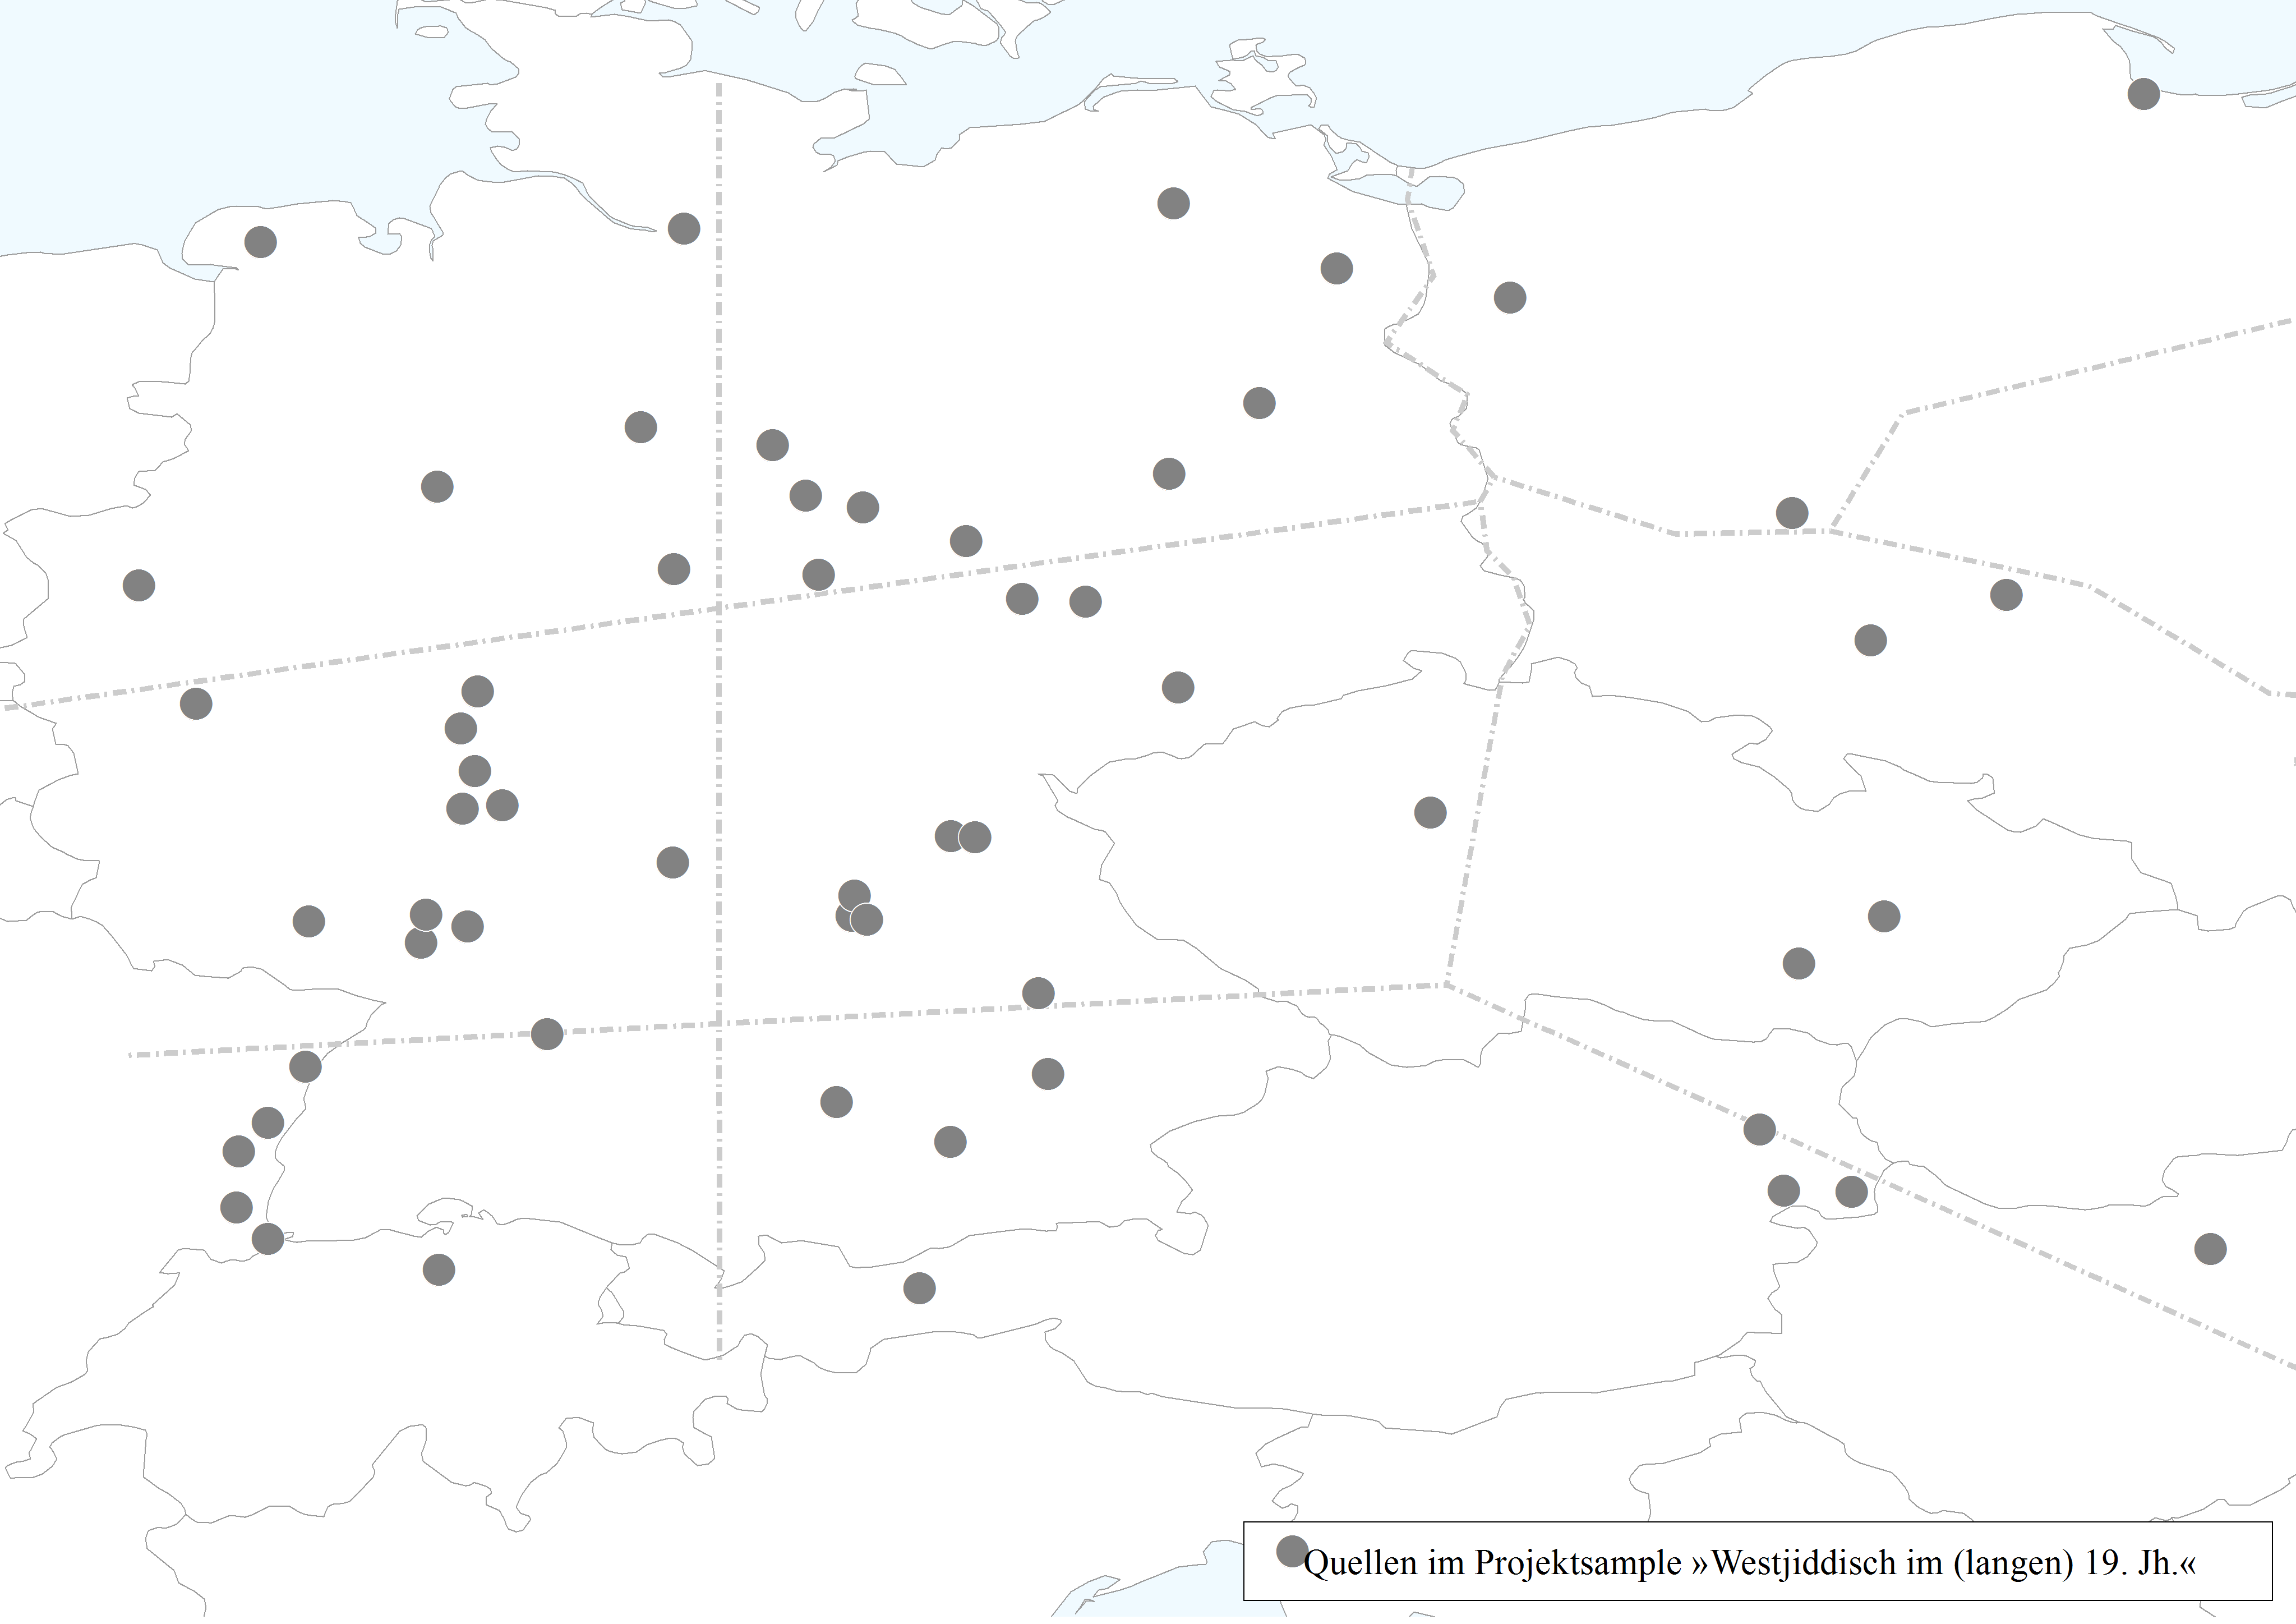
\includegraphics[width=\textwidth]{figures/quellengenerelldiss_sw.png}
		\caption{\label{kartegeo}Karte zur geographischen Verteilung des Projektsamples}
		\end{figure}
		\end{center}


%\noindent Die nachfolgenden  Beschreibungen der Westjiddischen Überlieferungsformen  (Kapitel \ref{Überlieferungsformen}) und der literarischen Verwendung des Jiddischen (Kapitel \ref{Kapitel Funktionstypen}) fußen auf den Ergebnissen des  Projektsamples, dessen aktuelle Version unter \url{http://www.online.uni-marburg.de/westjiddisch/index.php} einsehbar ist.  

Das Projektsample zeigt deutlich wie wichtig es ist den Wert nicht-jüdischer Quellen des späten Westjiddischen zu überprüfen, denn nur unter Zunahme dieses durchaus problematischen Datensatzes, ist es möglich quantitativ gesicherte Aussagen über sprachliche Strukturen des gesprochensprachlichen Westjiddischen zu treffen.


  \chapter{Untersuchungskorpus zum Literaturjiddischen} \label{korpora}
 % \epigraph{\textit{If you aren't taking a representative sample, you won't get a representative snapshot.}}{--- \textup{Nate Silver}}
% \epigraph{\textit{Any natural corpus will be skewed.}}{--- \cite[159]{Chomsky1957}}
% completes chomsky Zitat% \epigraph{\textit{Any natural corpus will be skewed. Some sentences won’t occur because they are obvious, others because they are false, still others because they are impolite. The corpus, if natural, will be so wildly skewed that the description would be no more than a mere list.}}{--- \textup{Noam Chomsky ([1957] 1962:159)}}
\noindent \ili{Literaturjiddisch} ist eine rein poetische  Varietät, keine natürliche Sprache. Obzwar es immer auf eine natürliche Sprache verweist (Jiddisch) und eingebettet ist in eine ebenfalls natürliche, wenn auch literarische Sprache (Deutsch), so unterscheidet sich ein \isi{Korpus}, bestehend aus literaturjiddischen Quellen, stark von anderen linguistischen Korpora. So ist in etwa der Vorwurf der Unvollständigkeit, den man jedem Textkorpus natürlicher Sprachen  vorhalten kann (vgl. insbes. \cite[159]{Chomsky1957}), im Falle des Literaturjiddischen haltlos: Über die literarische Überlieferung hinaus gibt es kein Zeugnis, da jenseits der Literatur kein \ili{Literaturjiddisch} bestehen kann. Jede literarische Figur eines jeden literarischen Textes legt uns bereits den Gesamtumfang ihrer Sprache dar. Aus linguistischer Perspektive haben wir es hierbei mit einem dankbaren Ausnahmefall zu tun. 

Die Recherchearbeit im Projekt \qu{Westjiddischen im (langen) 19. Jahrhundert} hat ergeben, dass \,%rs zum streichen
hauptsächlich literarische Quellen, zumeist Dramen, von vorwiegend christlichen Autoren überliefert sind (vgl.\, Abschnitt %linktomanuscript
\ref{sec:quellenkapitel}). Diese Texte entsprechen dem, was \cite{Richter1995} als \qu{Literaturjiddisch} definiert, da Jiddisch hier verschiedene literarische Funktionen trägt (vgl.\, Abschnitt \ref{Kapitel Funktionstypen}). Der Hauptfunktionstyp ist eine Mischform zwischen pejorativ und humoristisch (\hai{B2} \& \hai{C2}). Aufgrund dieser besonderen Datenlage besteht die Notwendigkeit, sich mit diesem speziellen Texttyp näher auseinanderzusetzen. Ausgehend von der im Projekt erarbeiteten Quellsammlung wurde gesondert ein \isi{Korpus} literaturjiddischer Texte der Typen \hai{B2}, \hai{C2} und \hai{D2} zusammengetragen und in Hinblick \,%rs r streichen
auf die darin vorkommenden sprachlichen Markierungen analysiert.\footnote{Da die Recherche nach literaturjiddischen Texten nicht im Zentrum des \hai{DFG}-Projekts stand, sondern die Recherche nach authentischen Quellen des Westjiddischen, erfasst das Projektsample wahrscheinlich einen geringen Ausschnitt dieses Quelltyps. Besonders aus der Mitte des 19. Jahrhunderts müssten noch deutlich mehr Quellen zu finden sein, als sie im Rahmen des Projektes erfasst wurden. Was diesen Quelltyp betrifft, sehen wir im Projektsample wohl nur die Spitze des Eisbergs. Für das Analysekorpus zum \hai{chrLiJi1} wurden zusätzliche Recherchen angestellt; dies gilt besonders für Fünfjahresintervalle, aus denen Quellen fehlten.} Dieses \isi{Korpus} zum christlichen \ili{Literaturjiddisch} im 19. Jahrhundert (\hai{chrLiJi1}) bildet das Kernkorpus dieser Arbeit.  

Die Texte des Kernkorpus haben gemeinsam, dass sie allesamt aus der Feder nicht-jüdischer Autoren stammen. Damit sind die darin auffindbaren Sprachdaten Information aus zweiter, wenn nicht sogar dritter Hand. Vorrangig aus diesem Grund wurde ein wesentlich kleineres Spezialkorpus zum \hai{jüdLiJi1} aufgebaut und analysiert (s. Abschnitt \,%rs Abschnitt ergänzen 
 \ref{spezialjüliji}). Ein solches macht darüber hinaus auch im Kontext einer diskursanalytischen Grundidee Sinn, da so geprüft werden kann, ob die Fremdwahrnehmung (\hai{chrLiJi1}) die Eigenwahrnehmung (\hai{jüdLiJi1}) beeinflusst oder nicht. 
  
  \section{Kernkorpus des nicht-jüdischen Literaturjiddischen im 19. Jahrhundert}\label{kernkorpus}
%\noindent
 Das Kernkorpus literaturjiddischer Texte der Funktionstypen \hai{B2}, \hai{C2} und \hai{D2} wurde nach folgenden Kriterien zusammengestellt:
 
 \begin{description}  
\item[\textbf{Diachrone} \textbf{Verteilung}] 
Auf der Zeitskala 1700–1950 wurden Fünfjahresintervalle gesetzt. Pro Intervall werden, sofern vorhanden, zwei Quellen analysiert.
\item [\textbf{Textsorte}] Dramen wurden bei der Auswahl bevorzugt, da diese zum einen unter den vorliegenden Textsorten den höchsten Grad konzeptioneller Mündlichkeit (nach \citealt{KochOesterreicher1985}) aufweisen, und da diese Textsorte zum anderen eine generell hohe Belegdichte aufweist. %linktomanuscript  (s. Abschnitt \ref{Verteilung Textsorten}).
\item [\textbf{Autorschaft}] Gesicherte nicht-jüdische Autorschaft.
\item [\textbf{Funktionstypen}] Es wurde versucht, das \isi{Korpus} in Bezug auf die Funktionstypen ausgewogen zu gestalten. Pro Intervall sollte je eine Quelle dem Typ \hai{B2} und eine dem Typ \hai{C2} angehören. Da eine Differenzierung zwischen \hai{B2} und \hai{C2} nicht immer einfach zu treffen ist, konnte dieses Kriterium nicht immer greifen. In dem Fall wurde versucht in einem Intervall mindestens eine Quelle, die eindeutig einem der beiden Typen \hai{B2} oder \hai{C2} zuzurechnen ist, aufzunehmen. Texte aus dem späten 19. und frühen 20. Jahrhundert dürfen auch dem \hai{D2}-Typ zugehören, sofern keine \hai{B2} oder \hai{C2} Quellen zur Verfügung standen. 
\item [\textbf{Sprechanteile jüdischer Figuren}] Sind pro Intervall mehrere potenzielle Quellen gegeben, werden die Quellen mit der höchsten Tokenfrequenz jüdischer Figurenrede gewählt.
\item[\textbf{Vermeidung gebundener Sprache}] Sofern es die Quellenlage erlaubt, werden Quellen in gebundener Sprache vermieden, da diese v.\,a.\, für die syntaktische Analyse u.\,U. ein verzerrendes Bild transportieren. 
\end{description}

Unberücksichtigt blieben bei der Korpusbildung die Faktoren der räumlichen Verteilung der Quellen und der Textlänge bzw. des Redeanteils jüdischer Figuren.\footnote{\label{FNSeitenzahlliji}Es wurde natürlich darauf Rücksicht genommen, Texte mit möglichst viel literaturjiddischen Sequenzen aufzunehmen, jedoch wurde das \isi{Korpus} nicht auf \quein{Normalseiten} (= 400 Wortformen pro Seite) skaliert (vgl.\, \qu{\citealt{Fnhdkorpus1972}} ). Die Zählung aller (physischen) \,%rs -n
 Seiten, die sprachlich relevante Daten zum \hai{chrLiJi1} liefern, ergab einen Gesamtumfang von 1181 Seiten. Eine durchschnittliche Quelle (Mittelwert) hat einen Umfang von 22,3 Seiten, liegt also grob betrachtet im Umfang der 30 Normalseiten, wie sie das \qu{Bonner Frühneuhochdeutschkorpus} verwendet. Wie man an der hohen Standardabweichung von 30,5 Seiten erkennt, ist das \isi{Korpus} extrem unausgewogen. Da die Texte in ihrem Umfang nicht skaliert wurden, sind Seitenzahlen generell weniger aussagekräftig und können keine Daten über die quantitative Verteilung eines Phänomens liefern. Die Angabe der Seitenzahlen erfüllt somit einen rein dokumentarischen Zweck, der die Korpusdaten überprüfbar macht.}  

Mit den angewandten Kriterien ist ein Textkorpus von 53 Texten entstanden, das zumindest den Zeitraum zwischen 1770 und 1875, immerhin 105 Jahre, lückenlos mit zwei Quellen abdeckt. Vor und nach diesem Zeitraum konnten nur vereinzelt relevante Texte in das \isi{Korpus} Eingang finden.
   
  \begin{figure}
\fittable{
	\begin{tikzpicture}
		\begin{axis}[ybar, width=1.02\textwidth,height=0.3\textheight,
		legend style={at={(1,1)},xshift=-13.25cm, yshift=-0.1cm,anchor=north west,nodes=left},
			%title={Funktionstypen des sp\"aten Westjiddisch},
			xtick={1700, 1725, 1750, 1775, 1800, 1825, 1850, 1875, 1900, 1925, 1950},
			x tick label style={ /pgf/number format/1000 sep=}, 
		y tick label style={/pgf/number format/1000 sep=},
			%extra y ticks={456.1, 1022.4},
			%extra y tick labels={{456,1},{1022,4}},
			extra y tick style={grid=major,
				tick label style={, ,}},
				ymin=0.1,
				bar width = 4pt,
				%ymax=5,
				ylabel={Quellen},
			enlarge x limits=0.03]		
			
				\addplot [fill=gray!20!white]  table [x=interval, y=kgesamt] {figures/kgesamt.txt};
						

			
			\legend{\hai{chrLiJi1}} %macht Legende
			
		\end{axis}			
	\end{tikzpicture}
}
	\caption{Quellenverteilung im \isi{Korpus} zum \hai{chrLiJi1}}\label{kgesamt}	
	\end{figure}



Ein Grund dafür, dass trotz intensiver Recherche vor 1770 und nach 1879 kaum Quellen vorliegen, kann sein, dass der sprachnormierende Diskurs über das Westjiddische in diesen Zeiten noch nicht bestand bzw. weitestgehend abgeschlossen war. Vom christlichen \ili{Literaturjiddisch} als eine kurzlebige \quein{Modeerscheinung} zu sprechen, ist, in Anbetracht der Datenlage, eine Untertreibung. Jüdische Figuren sprachlich zu markieren ist, wie Abschnitt \ref{westjiddistik} zeigt, ein über einen längeren Zeitraum etabliertes literarisches Mittel. Der Rückgang des Hebräischen zu Gunsten des Jiddischen als Zielsprache der \isi{Imitation} erlebt trotz vereinzelter Vorläufer in der ersten Jahrhunderthälfte des 18. Jahrhunderts erst ab den 1770ern seinen Durchbruch.%\footnote{Über die Recherchen im Projekt \qu{\ili{Westjiddisch} im (langen) 19. Jahrhunderts} hinaus, wurden zahlreiche Bemühungen angestellt, Texte des 16., 17., 18. und 20. Jahrhunderts ausfindig zu machen. Wie das \isi{Korpus} zeigt ohne viel Erfolg.} In dieser Zeit beginnt auch die Debatte um Sprachnormierung und die Aufgabe des Jiddischen zu Gunsten des Deutschen. Für die Zeit nach 1879 kann angenommen werden, dass \ili{Westjiddisch} bereits in den meisten Gegenden stark geschwunden ist. %Wie die Analyse der Quellen zeigt (s. Abschnitt \ref{analysen}), setzt hier allmählich ein Eindringen des Ostjiddischen in das \ili{Literaturjiddisch} ein, was den bereits fortgeschrittenen Rückgang des Westjiddischen in dieser Zeit bestätigen würde.   

Wie beabsichtigt machen Dramentexte den größten Anteil aus; jedoch mussten auch andere Textsorten und Quellen in gebundener Sprache aufgenommen werden (s. Tabelle \ref{tbltextsortenliji}). Für die Zeitabschnitte
 1725–1749 und 1840–1844 konnten nur lyrische Texte gefunden werden.
  
  
  %%Tablle chr\ili{LiJi1}
	\begin{table} 
	
		\begin{tabularx}{\textwidth}{ccccc}
		\lsptoprule
	  \textbf{Quellen (gesamt)}  &	 \textbf{Dramen} 	&  \textbf{Prosatexte}	&	\textbf{lyrische Texte}	&	\textbf{Sammlungen}	 \\ \midrule % horizontale Trennlinie
			  53 	&	34	&	6	&	9	&	4 \\
			 100\%  	&	64,15\% &	11,32\%	& 	16,98\%	&	7,55\%\\
			 \lspbottomrule
		 \end{tabularx}
		 \caption{\label{tbltextsortenliji}Textsorten im \isi{Korpus} zum \hai{chrLiJi1}}
		 
		 \end{table}
	 	


% \todo{Legende ragt in Diagramm hinein; Verlorener Satz zwischen Diagramm und Tabelle; Bekomme sie nicht bewegt :-O}
  %%%Diagramm gesamt korpus textsorten
  \begin{figure}[p]
\fittable{
	\begin{tikzpicture}
		\begin{axis}[cycle list name =linestyles*, width=0.9\textwidth,height=0.3\textheight,
		legend style={at={(1,1)},xshift=0.2cm, yshift=0cm,anchor=north west,nodes=left},
			%title={Funktionstypen des sp\"aten Westjiddisch},
			xtick={1700, 1725, 1750, 1775, 1800, 1825, 1850, 1875, 1900, 1925, 1950},
			x tick label style={ /pgf/number format/1000 sep=}, 
		y tick label style={/pgf/number format/1000 sep=},
			%extra y ticks={456.1, 1022.4},
			%extra y tick labels={{456,1},{1022,4}},
			extra y tick style={grid=major,
				tick label style={, ,}},
				ymin=0.1,
				%ymax=5,
				ylabel={Quellen},
			enlarge x limits=0.03]			
				\addplot [very thick] table [x=interval, y=kdramen] {figures/kdramen.txt};
		\addplot  [very thick, color=gray!40!white] table [x=interval, y=kprosa] {figures/kprosa.txt};
\addplot  [dotted, very thick] table [x=interval, y=ksammlung] {figures/ksammlung.txt};
\addplot  [dotted, very thick, color=gray!40!white] table [x=interval, y=klyrik] {figures/klyrik.txt};
		
			\legend{Dramen, Prosa, Sammlung, Lyrik} %macht Legende
				
		\end{axis}
	\end{tikzpicture}
}
	\caption{Diachrone Verteilung der Textsorten im \isi{Korpus} zum \hai{chrLiJi1}}
	\label{ktextsorte}	
	\end{figure}

Die diachrone Verteilung der Textsorten (Abbildung \ref{ktextsorte}) zeigt, dass sich zwischen 1770 und 1820 immerhin ein auf 25 Jahre erstreckendes Kontinuum ausschließlich dramatischer Quellen ergibt. Nach dieser Phase ist das \isi{Korpus} ein Gemisch verschiedener Textsorten. So lässt sich das \isi{Korpus} auf Grundlage % rs  auf Grundlage
der Textsortenverteilung in drei Abschnitte unterteilen:  im ersten Abschnitt (1700–1769) haben wir nur wenige, lyrische und epische Texte, in Abschnitt 2 (1770–1820) sind ausschließlich dramatische Quellen gegeben, während im dritten Abschnitt (1825–1949) eine große Textsortenvielfalt vorliegt. Dies muss bei der Analyse berücksichtigt werden.

 
Eine erneute, genauere Durchsicht der Texte ermöglichte eine Zuordnung der im Projektsample unter dem Mischtypus \hai{B2}/\hai{C2} laufenden Quellen als \hai{B2}- oder \hai{C2}-Quelle. Die Verteilung der Funktionstypen ist damit im Korpussample mehr oder weniger ausgeglichen (s. Tabelle \ref{tblfunktionstypenliji}). Die Typen \hai{B2} und \hai{C2} haben den größten Anteil. In nur drei Fällen musste auf Quellen des Typs \hai{D2} zurückgegriffen werden.\footnote{Diese drei Texte sind \hai{UT} (Stavenhagen, 1862), \hai{JD} (Wien, 1866) und \hai{AK} (Zürich, 1948).} In fünf Fällen konnte trotz intensiver Lektüre nicht entschieden werden, ob der \hai{B2}- oder der \hai{C2}-Typ vorliegt.\footnote{Dies betrifft die Quellen \hai{FL} (Mannheim, 1778), \hai{PF} (Augsburg, 1816), \hai{LP} (Brünn, 1849), \hai{FM} (Leipzig, 1852) und \hai{MV} (Berlin, 1862).}

 %%Tablle chr\ili{LiJi1} Funktionstypen
	\begin{table}[p]
	 
		\begin{tabularx}{\textwidth}{cCCCC}
		\lsptoprule
	\textbf{ Quellen (gesamt) } &	 \textbf{\hai{B2} }	&\textbf{ \hai{C2}}	&	\textbf{\hai{B2}} \& \textbf{\hai{C2}}	&	\textbf{\hai{D2}}	 \\ \midrule % horizontale Trennlinie
			  53 	&	24	&	21	&	5	&	3	 \\
			  100\% & 45,28\% & 39,62\% & 9,43\% & 5,66\% \\ 
\lspbottomrule
		 \end{tabularx}
		 \caption{\label{tblfunktionstypenliji} Verteilung der Funktionstypen im \isi{Korpus} zum \hai{chrLiJi1}}
		 
		 \end{table}
	 	

 
\begin{figure}[p]
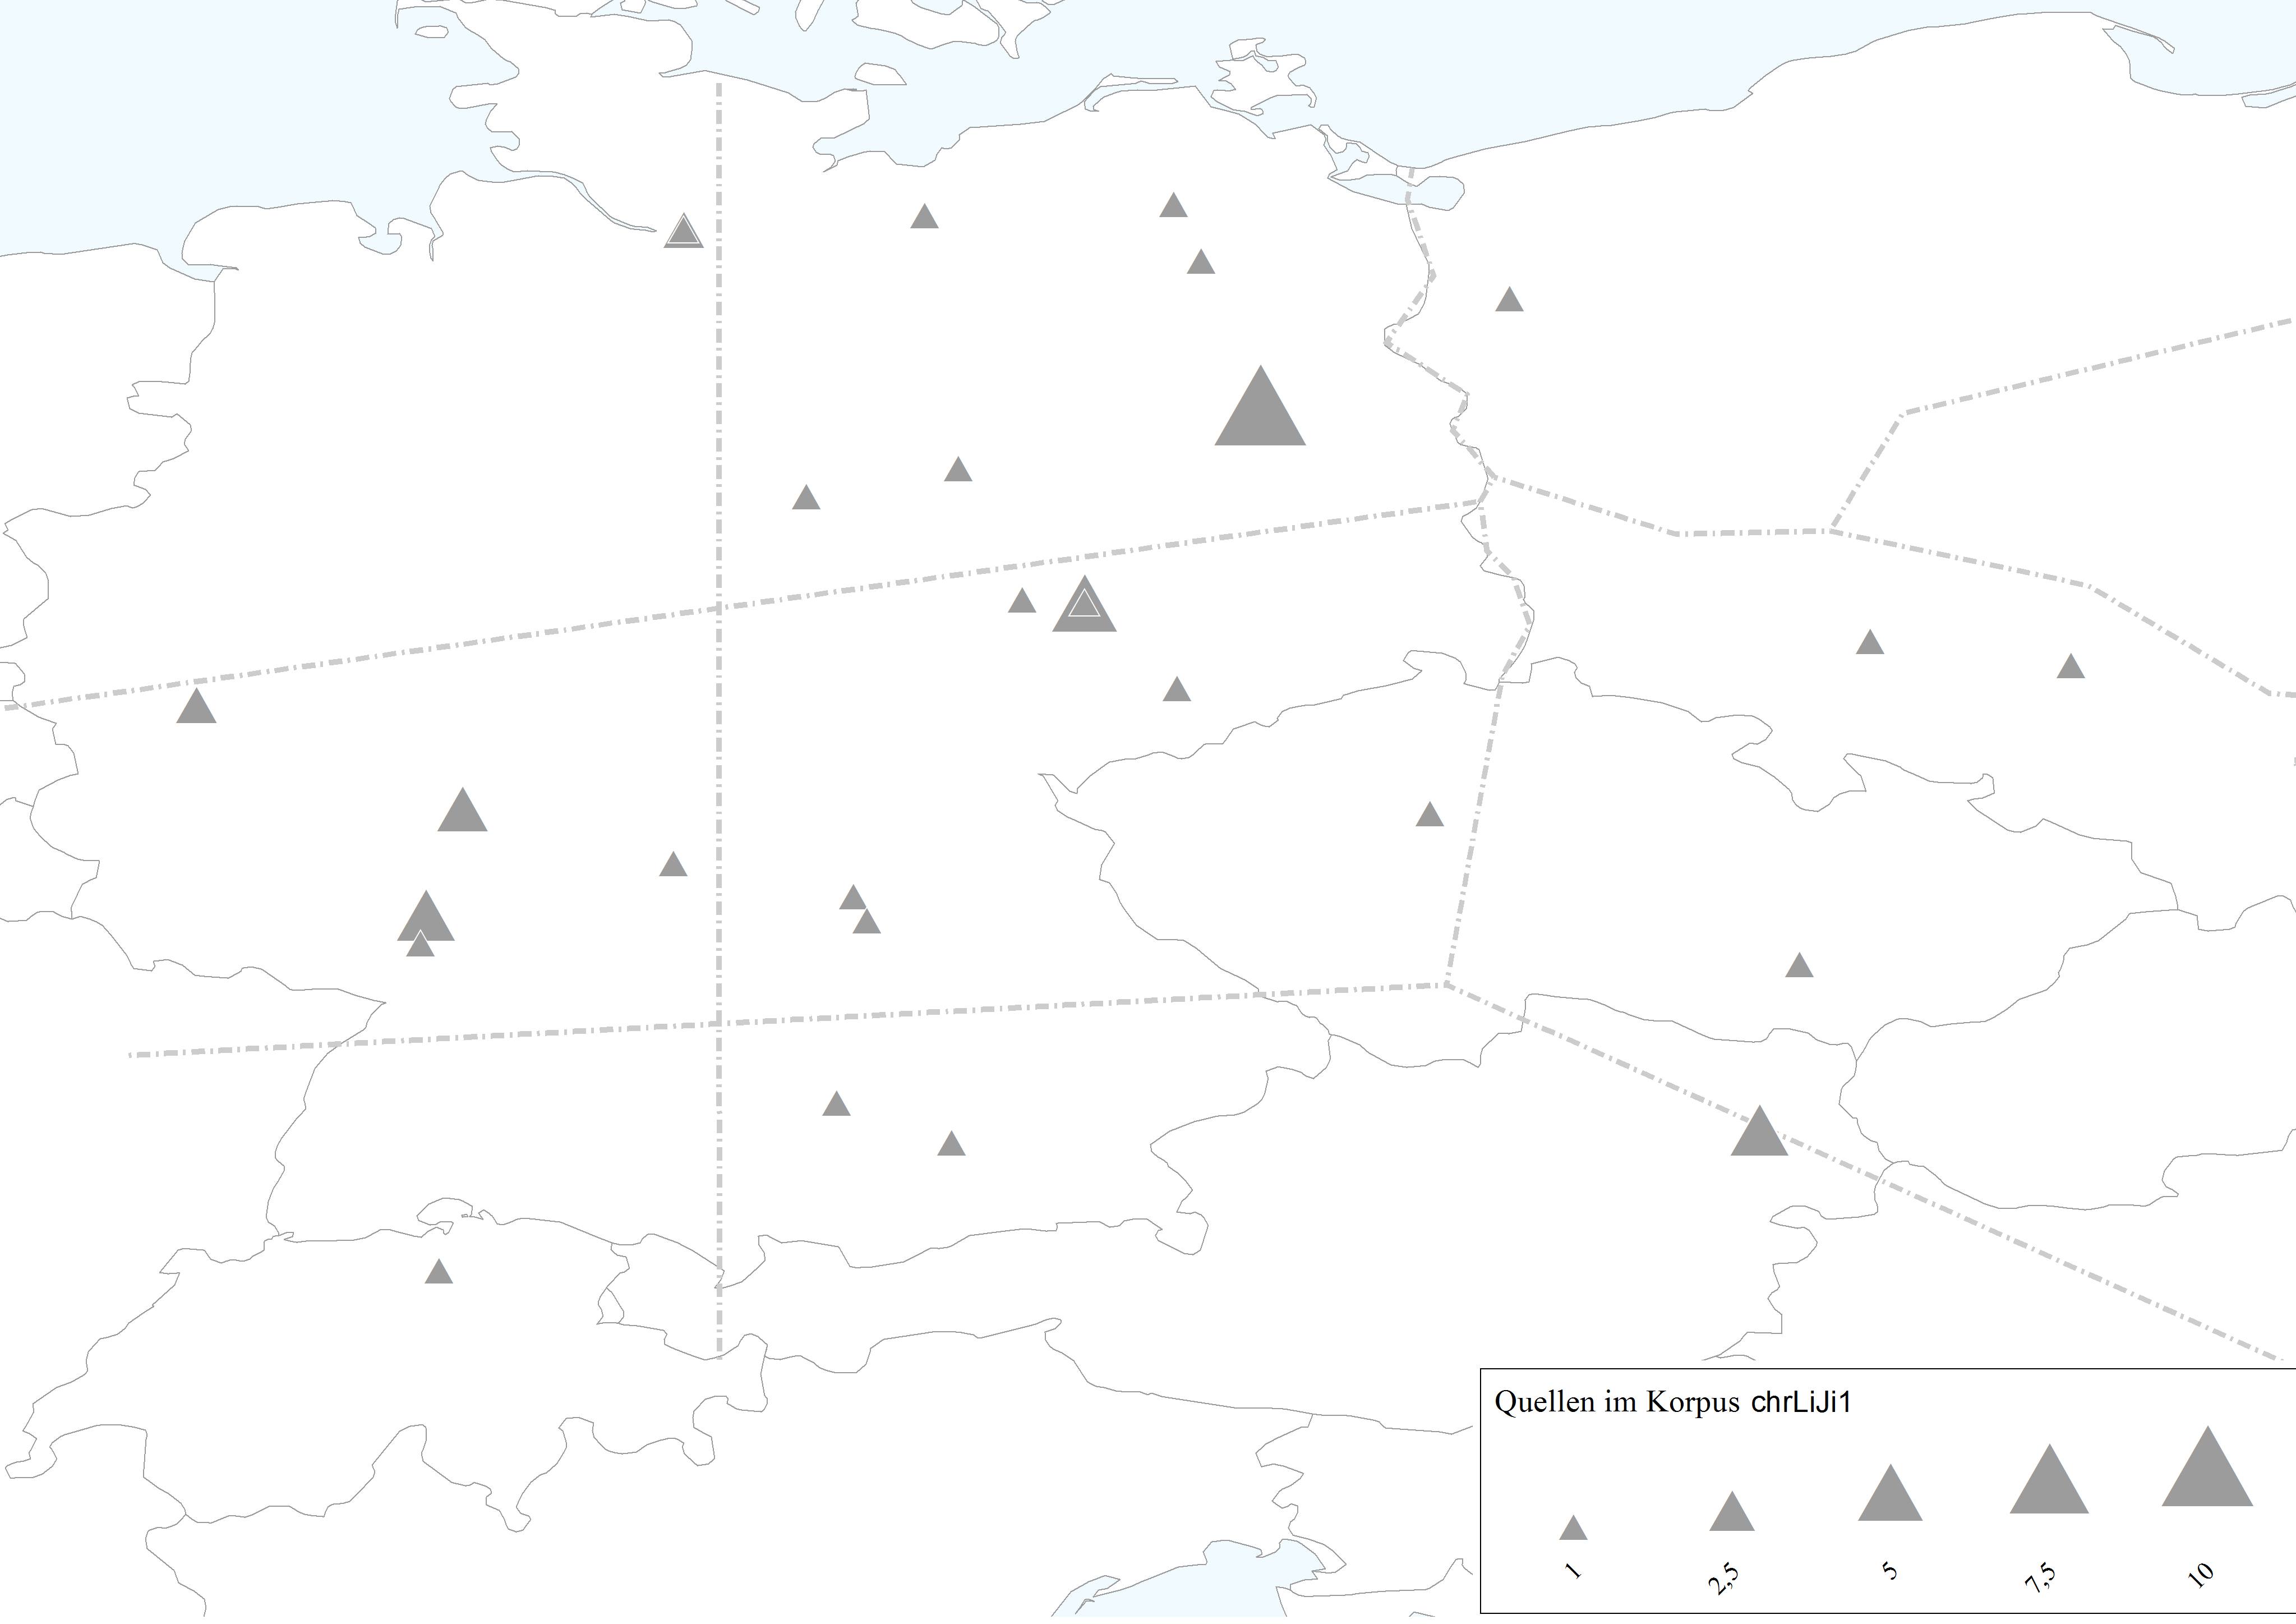
\includegraphics[width=\textwidth]{figures/liji1_menge3_diss_sw.png}
		\caption{\label{karteliji1menge} Karte zur quantitativen Verteilung des \isi{Korpus} \hai{chrLiJi1}}
		\end{figure}

 
Die räumliche Verteilung spielte bei der Korpusbildung keine Rolle. Wie die Kartierung der Korpusquellen zeigt (Abbildung \ref{karteliji1menge}),\footnote{Auch hier konnten nicht alle Texte einem Ort zugewiesen werden, vgl.\, Fn. \ref{FNkarte}, S.\, \pageref{FNkarte}. Insgesamt konnten 51 Quellen in die Kartierung aufgenommen werden.} entspricht dies der räumlichen Streuung des Projektsamples (vgl.\, Abbildung \ref{kartegeo}). Auch die quantitative Verteilung des \hai{chrLiJi1}-\isi{Korpus} (Abbildung \ref{karteliji1menge}) zeigt mit den Zentren Berlin, Leipzig, Wien, Frankfurt und Mannheim ähnliche Strukturen wie die des Projektsamples (vgl.\, \citealt[64, Abbildung 4.16]{SchaeferDiss}). Die im Projektsample besser abgedeckten Regionen des westl. \hai{{\NWJ}} und des nördlichen Übergangsgebiets sind im \hai{chrLiJi1}-\isi{Korpus} nur durch einzelne Quellen aus den Grenzgebieten repräsentiert. 





  
  %\clearpage
  Es sei erwähnt, dass in drei der aufgenommenen Texte Jiddisch nicht in Relation zum (Hoch-) Deutschen, sondern zu niederdeutschen Dialekten steht. Die entsprechenden Quellen sind \hai{UT} (Stavenhagen, 1862; Mecklenburgisch), \hai{DK} (Osterwieck, 1872; Ostfälisch) und \hai{DP} (Pyrzyce, 1874; westl. Ostpommersch). Die Analyse wird zeigen, ob in einer niederdeutschen Umgebung andere Strategien zur \isi{Emulation} des Jiddischen verwendet werden als in einer hochdeutschen.
  
Zwei Autoren sind im \isi{Korpus} mehrfach vertreten: Von Julius v. Voß wurden drei Dramen (\hai{EV} Berlin, 1817; \hai{NW} Berlin, 1804; \hai{PS} Berlin, 1808) und von Louis Angelt zwei Dramen (\hai{AJ} Berlin, 1825 u. \hai{PP} Berlin, 1839) ausgewertet. Dies könnte einerseits das Bild etwas verzerren, andererseits hat es den Vorteil, dass diese Autoren gesondert analysiert werden können, um zu prüfen, wie homogen sie sich im Textvergleich verhalten.\footnote{Wie die Clusteranalyse der Quellen zeigt (vgl. Abbildung \ref{boxplotcluster}, S. \pageref{boxplotcluster}), verhalten sich die jeweiligen Quellen trotz identischer Autorschaft unterschiedlich, was die Verteilung der verwendeten liji Phänomene betrifft. Ausgehend von dieser Clusteranalyse scheint auch die Matrixsprache (Hochdeutsch vs. Niederdeutsch) keinen entscheidenden Einfluss zu nehmen.}


 \section{Spezialkorpus des jüdischen \ili{Literaturjiddisch} im 19. Jahrhundert} \label{spezialjüliji}
%  %\noindent
 Um einen Eindruck zu erhalten, ob und wie der literarische Diskurs zum Jiddischen konfessionelle Unterschiede aufweist, wurde ein kleines Spezialkorpus zu literaturjiddischen Quellen jüdischer Autoren angelegt. Besonders interessant, da mit interkonfessioneller Leserschaft zu rechnen ist, sind Texte vom Funktionstyp \hai{C1}.\footnote{In zwei Fällen (PBerlin1 u. PBerlin2) besteht die Möglichkeit, dass diese Texte auch christlichen Autoren zuzuschreiben sind und damit dem Mischtyp \hai{C1}/\hai{C2} angehören. Diese Texte werden darum mit besonderer Vorsicht behandelt.} Darunter fallen fünf Bände der \qu{Gedichte und Scherze in jüdischer Mundart}\footnote{Von diesen Sammlungen jüdischer Witze und Anekdoten sind 23 Bände bekannt (vgl.\, \citealt{Gruschka2003}). Für das \isi{Korpus} wurden Bd. 1 und Bd. 23, sowie in Fünfer-Intervallen, die Bde. 5, 10 und 15 gewählt. Die zeitliche Verortung dieser Hefte ist jedoch heikel, da die Erstausgaben kaum mehr erhalten sind. Die Periode der Erstveröffentlichungen lässt sich auf den Zeitraum zwischen 1850 und 1870 eingrenzen. Bis in die 1870er Jahre hinein wurden die Hefte von Eduard Bloch in Berlin herausgegeben, dann aber nur mehr Reproduktionen.} und fünf Texte, die man als politische Pamphlete charakterisieren kann. Das \isi{Korpus} deckt den Zeitraum zwischen 1848 und 1877 ab.\footnote{Das \isi{Korpus} zum \hai{jüdLiJi1} umfasst 73 Seiten bei einem Mittelwert von 7 Seiten pro Quelle. Die Standardabweichung liegt bei 3 Seiten in einem noch relativ angemessenem Bereich (vgl.\, Fn. \ref{FNSeitenzahlliji} S.\, \pageref{FNSeitenzahlliji}).} Überwiegend haben diese Texte in Berlin ihren Ursprung bzw. waren im großstädtischen Raum verbreitet (\citealt{Gruschka2003}).\footnote{Die \hai{GuS} sind alle in Berlin gedruckt, ebenso die Pamphlete \hai{PBerlin1} und \hai{PBerlin2}. Die zahlreichen Pamphlete des Isaac Moses Hersch, von denen eines Eingang in das \isi{Korpus} gefunden hat (\hai{PAlsleben}), werden wahrscheinlich auch eher im großstädtischen Raum rezipiert worden sein als im Heimatort des Autors Alsleben. Die beiden weiteren Pamphlete stammen aus dem Gebiet des \hai{{\SÜJ}} mit Breslau (\hai{PBreslau}) und Debrecen (\hai{PDebrecen}). Letztere Quelle ist ein besonders interessantes Beispiel für ungarisches \hai{{\LiJi}}.}  	
    
  	\begin{table} 
 		\begin{tabular}{ccc}
\lsptoprule
	\textbf{Quellen (gesamt)  }&\textbf{GuS} 	&  \textbf{Pamphlete}	\\ 
\midrule 
			  10 	&	5	&	5	 \\
			  	&	ca.\, 1850er–1870er & 1848--1876\\ 
\lspbottomrule
		 \end{tabular}
		 \caption{\isi{Korpus} \hai{jüdLiJi1}}
		 \label{tbljüliji}
		 \end{table}
	 	
 Tatsächlich hätte ein \isi{Korpus} zum \hai{jüdLiJi1} deutlich umfangreicher ausfallen können. Dass hier nur zehn Texte Eingang gefunden haben, ist eindeutig nicht der Datenlage geschuldet, %linktomanuscript (vgl.\, Diagramm in Abbildung \ref{juedQuellen}), 
 sondern dem Fokus der Arbeit auf die \quein{\isi{Imitation} des Jiddischen} und dem literarischen Diskurs. Ziel der Korpora dieser Arbeit ist es nicht, möglichst authentische Quellen des Westjiddischen zusammenzutragen, sondern eben jene Quellen heranzuziehen, die besonders stark durch den kulturellen Diskurs beeinflusst  und damit möglichst weit entfernt von der Sprachwirklichkeit anzusiedeln sind. Die hier aufgenommenen Texte des \hai{jüdLiJi1} sind Quellen des assimilierten Judentums und Belege dafür, dass die \isi{Assimilation} nicht nur sprachlich, sondern auch formen- und literatursprachlich zur Jahrhunderthälfte stark fortgeschritten war.

  

                   
 \section{Methodik}\label{erhebungsmethode}


Die in den Korpora zusammengestellten Texte wurden einer Datenerhebung unterzogen, in welcher jeder Text händisch durchgegangen wurde und die darin vorkommenden sprachlichen Markierungen jüdischer Figurenrede in eine Phänomenmaske (s. Tabellen \ref{maske1} -- \ref{maske4}) eingetragen wurden.\footnote{Die in diese Maske aufgenommenen Phänomene ergeben sich aus den Daten selbst. Sie hat sich damit im Laufe der Datenerhebung herausgebildet und wurde nicht im \isi{Vorfeld} festgelegt. Aufgenommen wurde zunächst alles, was von der Schriftsprache abweicht. Die sprachlichen Abweichungen von der Literatursprache (Deutsch) mussten dazu selbstverständlich für mich selbst erkennbar und kategorisierbar und damit sprachwissenschaftlich \textit{salient} sein.} Zusätzlich wurden folgende Metadaten zu jedem Text angelegt:
 
 
 \begin{quote}
	 Titel [Kürzel],\footnote{Die Vergabe der Kürzel folgt der Regel: Quellen des christlichen \hai{{\LiJieins}} zwei Großbuchstaben, \hai{jüdLiJi1} Quellen der \qu{Gedichte und Scherze in jüdischer Mundart} als GuS+‘Nr. der jew. Ausgabe', Pamphlete des \hai{jüdLiJi1}-\isi{Korpus} werden mit P+‘Ort' abgekürzt. \,%rs Spatium fehlt
	Um einen leichteren Zugang zu ermöglichen, werden im Fließtext und in Sprachbeispielen die Kürzel zum \hai{chrLiJi1} um Erscheinungsort und Erscheinungsjahr ergänzt.\\
    Die Kürzel der untersuchten Quellen werden im Anhang (S. \pageref{appendixchrliji1}, \pageref{appendixjuedliji1}) %RS Klammer fehlt
 aufgeschlüsselt.} Autorenname, Erscheinungsjahr \\  Untertitel, Erscheinungsort, Verlag, Ausgaben 
Textsorte, Funktionstyp, Dia\-lektregion nach \cite{Katz1983} (falls ermittelbar)
Besondere Hinweise zu Inhalt u. Autor
 \end{quote}
		 
 Die Daten wurden bei der Eingabe in die Phänomenmaske auf maximal fünf Tokens pro Lexem (Lexik, Phonologie u. Graphie) bzw. pro Phänomen (im Fall von \isi{Morphologie} u. \isi{Syntax}) skaliert, so dass es möglich war, auch umfangreichere Texte aufzunehmen.  Ebenfalls der Skalierungsidee geschuldet ist der Umstand, dass jeder Beleg nur einmal pro Seite zitiert wurde, und zwar auch, wenn dieser mehr als einmal auf einer Seite vorliegt. Das heißt, jedes Datum ist mindestens einmal auf einer Seite belegt, die Belegzahlen sind aber nicht als absolute Werte zu verstehen. 
 
 Nicht erhoben wurden metasprachliche Laienurteile, wie z.\,B.\, in (\ref{bspmajorat}), da dieser Arbeit an der Erhebung grammatischer Formen der sprachlichen \isi{Imitation} gelegen ist und nicht an den sprachpolitischen Diskursen ums Jiddische.

 
  \eenumsentence{
	\item [] […] \textit{und nun erschallte hinter ihm ein fürchterliches Rabengekrächze aus dem Munde der alten Jüdin. In halb hebräischen Schimpfreden und im verzerrtesten Judendialekt zeihte sie die arme Tochter der Unkeuschheit,} […] \\ (\citealt[45]{Arnim1962}) 
\label{bspmajorat} 
}


Für das weitere Vorgehen wurden die Ergebnisse der Datenerhebung in das Programm \textsc{AntConc}\footnote{Diese Kon­kor­danz-Software wird unter \url{http://www.antlab.sci.waseda.ac.jp} zur freien Verfügung gestellt.} geladen und mit dessen Hilfe der näheren Analyse unterzogen. %Zur Darstellung der Analyseergebnisse werden im Folgenden Histogramme, Karten und Tabellen genutzt. 
Die erhobenen Daten aller Korpora finden sich im Appendix von \citet{SchaeferDiss}. %linktomanuscript
In den nachfolgenden Analysen der Einzelphänomene werden einzelne illustrierende Belege angeführt. Nur in einzelnen Fällen sind die im Text gegebenen Beispiele exhaustiv; in diesen Fällen wird dies explizit genannt. 

Die hier vorliegende Arbeit möchte einen ersten groben Überblick bieten, wie sprachliche \isi{Imitation} funktioniert. Demnach können in den Analysen singulär auftretende Einzelphänomene nur exemplarisch ausgewertet werden. Abstriche bei der Phänomenanalyse finden sich v.\,a.\, im lexikalischen Bereich und bei singulären phonologischen Phänomenen wieder. Prinzipiell wurde jedes Phänomen einer Detaillanalyse unterzogen, das in minimal vier Quellen des \hai{chrLiJi1} auftritt oder zumindest mit frequent auftretenden Manipulationsstrategien verwandt ist. 

\begin{table}
        \caption{Phänomenmaske Lexik}\label{maske1} 
        \begin{tabularx}{\textwidth}{lQQ}
	\lsptoprule
   &  \textbf{Phänomen}& \textbf{Beispiel}\\ 
\midrule 
	 	&Kennwörter {WJ} & \textit{Ette} \sem{Vater}, \textit{Mamme} \sem{Mutter}\\
 			& Kennwörter {OJ} & \textit{Tate} \sem{Vater}, \textit{Mame} \sem{Mutter} \\
 			& Hebraismen & \textit{Adonay} \sem{der Ewige}, \textit{Ische} \sem{Frau}\\
 			& Psychoostentative Ausdrücke & \textit{Wei geschrien!} \sem{Weh geschrien!}\\
 			& Sonstiges & \textit{heißt} \sem{nennt}, \textit{als} \sem{wie}\\
\lspbottomrule
\end{tabularx}
\end{table}

\begin{table} 
        \caption{Phänomenmaske Morphologie}\label{maske3} 
        \begin{tabularx}{\textwidth}{lQQ}
	\lsptoprule
    &  \textbf{Phänomen}& \textbf{Beispiel}\\ \midrule 
&	 {Diminution}\is{Diminution} (Singular; Plural) & \textit{Vögile} \sem{Vogel}, \textit{Madlich} \sem{Mädchen}\\
& Verbklasse \& Verbflexion & \textit{sennen} \sem{sie sind} \\
&Kasus bei vollen Obj.; Kasus n. Präp.; Kasus bei Pron.& \textit{Ich hob getroffen Menschen aus die ganze Welt } \sem{ich habe Menschen aus der ganzen Welt getroffen}\\
&Sonstiges&\textit{gespaziert} \sem{spaziert}\\ 
\lspbottomrule

\end{tabularx}
\end{table}

\begin{table}
        \caption{Phänomenmaske   Phonologie}\label{maske2} 
        \begin{tabularx}{\textwidth}{QQ}
	\lsptoprule
\hai{V24} (E\textsubscript{4} = {\mhd} \textit{ei}) > /a\textlengthmark/, /ɛ/ & \textit{Bahn} \sem{Bein}, \textit{kä} \sem{kein}\\
\tablevspace
\hai{V44} (O\textsubscript{4} = {\mhd} \textit{ou}) > /a\textlengthmark/ & \textit{kafen} \sem{kaufen}, \textit{Fra} \sem{Frau}\\
\textit{a}-Verdumpfung & \textit{hot} \sem{hat}, \textit{Tog} \sem{Tag}\\
\tablevspace
\hai{V22} (E\textsubscript{2} = {\mhd} \textit{ê}, \textit{œ}) > /ei/, /ai/ & \textit{seihe} \sem{sehe}, \textit{Keinik} \sem{König}\\
\tablevspace
\hai{V42} (O\textsubscript{2} = {\mhd} \textit{ô}) > /ou/, /au/& \textit{grous} \sem{groß}, \textit{waul} \sem{wohl}\\
\tablevspace
 \hai{V34} (I\textsubscript{4} = {\mhd} \textit{iu}) > <ei>, <ai>& \textit{neilich} \sem{neulich}, \textit{Leite} \sem{Leute}\\
\tablevspace
 Entrundungen (nhd. <ü>, <ö> > <i>, <e>)& \textit{ferchte} \sem{fürchte}, \textit{Mih} \sem{Mühe} \\
\tablevspace
{Palatalisierung}\is{Palatalisierung} /u\textlengthmark/ > /y/, /y\textlengthmark/& \textit{herüm} \sem{herum}, \textit{dü} \sem{du}\\ 
\tablevspace
Sproßvokal& \textit{Milich} \sem{Milch}\\
\tablevspace
<ai> für <ei>; <ey> für <ei>& \textit{haißt} \sem{heißt}, \textit{eyn} \sem{ein}\\
\tablevspace
ç > ʃ &\textit{nischt} \sem{nicht}\\
\tablevspace
<z> für <s>; <ß> für <s>; <ß> für <z>; <scht> für <st>& \textit{Zunne} \sem{Sonne}, \textit{ßag} \sem{sag}, \textit{ßu} \sem{zu}, \textit{Schtein} \sem{Stein}\\
\tablevspace
Konsonantismus \is{Konsonantismus} (diverses)& \textit{Köp} \sem{Kopf}, \textit{kegen} \sem{gegen}\\
\tablevspace
Sonstiges&\textit{schlage} \sem{schlagen}, \textit{et} \sem{es}\\
 \lspbottomrule
\end{tabularx}
\end{table}




\begin{table}
        \caption{Phänomenmaske Syntax}\label{maske4} 
        \begin{tabularx}{\textwidth}{QQ}
	\lsptoprule 
\hai{NP-Ex}; \hai{PP-Ex}; \hai{AP-Ex}; \hai{AdvP-Ex} & \textit{Bin ich gewesen in e Wein-Lokal} \sem{Bin ich in einem Weinlokal gewesen}\\
\tablevspace
\hai{VR} (zweigliedrig)& \textit{wo er soll essen} \sem{wo er essen soll}\\
\tablevspace
\hai{VR} (min. dreigliedrig)& \textit{as kein Buch darf vardorben werden} \sem{dass kein Buch verdorben werden darf}\\
\tablevspace
\hai{VPR}& \textit{daß er sich soll ahnen neien kahfen} \sem{dass er sich einen neuen kaufen soll}\\
\tablevspace
\hai{V2}& \textit{ass De bist still un ruhig} \sem{dass du still und ruhig bist}\\
\tablevspace
\hai{no-IPP}& \textit{Wie ich hob gewollt aheim gehen} \sem{Als ich habe heim gehen wollen}\\
\tablevspace
\isi{Relativpartikel}& \textit{ä Schnorrer, was is rumgelahfen in de Stadt} \sem{ein Bettler, der in der Stadt herumläuft}\\
\tablevspace
\isi{Negationskongruenz} \& -spreading & \textit{ber ßu sahnem Glicke hat's Kahner nicht gehert} \sem{zu seinem Glück hat es keiner gehört}\\
\tablevspace
\textit{kumen} + Bewegungsverb\textsubscript{\textit{zu}-Infinitiv}& \textit{Was kimmt ze geihn geritte?} \sem{Was kommt da geritten?}\\
\tablevspace
Sonstiges &\textit{eine Frage tun} \sem{fragen}\\
\lspbottomrule
\end{tabularx}
\end{table}
			
\part{Analysen} \label{analysen}  
\chapter{Lexikalische Markierungen}\label{lexikliji1}
 %\noindent
 Die folgende Analyse lexikalischer Markierungen strebt keine vollständige Beschreibung aller zu findenden Phänomene an, sondern will lediglich einzelne, besonders interessante und relevante Strategien sprachlicher Imitationen vorstellen, mit denen literaturjiddische Texte auf lexikalischer Ebene arbeiten.
 
 Eine Auswertung der Daten kann 
% nur
lediglich
 unter qualitativen Gesichtspunkten erfolgen. Komplexe quantitativ-statistische Analysen 
erlaubt das \isi{Korpus} kaum.
%  ist mit dem Korpus kaum möglich. %\todo{paraphrasiert}
 Dennoch wird versucht über die Tokenfrequenz bestimmter Phänomene quantitative Ergebnisse zu liefern. In Fällen lexikalischer Fragestellungen kann mit Hilfe von Frequenzklassen (\hai{{\FK}}),\footnote{Oft auch als \qu{logarithmic bins} oder \qu{Häufigkeitsklassen} bezeichnet.} basierend auf den Daten des \qu{Häufigkeitswörterbuch[s] gesprochener Sprache} (\citealt{Ruoff1981}), geprüft werden, ob ein frequenzbedingter Einfluss vorliegt. \citeauthor{Ruoff1981}s (\citeyear{Ruoff1981}) Daten zur deutschen Umgangssprache im Südwesten Deutschlands basieren auf dem Zwirnerkorpus.\footnote{Das unter der Leitung Eberhard Zwirnes zwischen 1955 und 1970 aufgebaute \isi{Korpus} von \qu{Schallaufnahmen aller deutschen Mundarten} ist über das Institut für Deutsche Sprache (\hai{IDS}) digital dokumentiert und zugänglich: \url{http://agd.ids-mannheim.de/download/korpus/Korpus_ZW_extern.pdf} [Stand: September 2014].} Ruoff berücksichtigt die Trennung nach Wortarten, die für die Berechnung der Tokenfrequenzen aufgehoben wurde. Dies ermöglicht zum einen den Vergleich mit \hai{{\FK}}n anderer Korpora, wie etwa denen des Deutschen Referenzkorpus (\hai{DeReKo}, 2012). Die Berechnung von Frequenzklassen erfolgt nach der Formel:\footnote{Die hier verwendete Formel folgt den Richtlinien des Institut für Deutsche Sprache (IDS) (\citealt[13]{DeReKo}). Die Gaußklammer bewirkt, dass das Ergebnis auf ganze Zahlen gerundet wird. Die Höhe des Ergebnisses bestimmt die Frequenzklasse.} 



\begin{center}\begin{math}
\hai{{\FK}} = \lfloor	log_2~ (\frac{Tokenfrequenz~des~untersuchten~Wortes}{Tokenfrequenz~des~häufigsten~Wortes}) + 0.5\rfloor 
\end{math}
\end{center} 
 

\largerpage
In Klasse 0 steht das häufigste Wort. Von 0 aufsteigend 
ist die \isi{Frequenz} pro Klasse abnehmend; d.\,h. Wörter der \hai{FK3} haben eine geringere Häufigkeit als Wörter der \hai{FK2}. Im Nenner der Formel zur Berechnung der \citeauthor{Ruoff1981}schen \hai{{\FK}}n steht der Wert 37536 für die Tokenfrequenz des häufigsten Lemma \sem{der/dieser} (vgl. \citealt[514–516]{Ruoff1981}). Die maximal erreichbare \hai{{\FK}} im \isi{Korpus} von \citealt{Ruoff1981} ist die \hai{FK15}. Das deutlich umfangreichere \hai{DeReKo} (2012) geht immerhin bis zur \hai{FK29} (vgl. Tabelle \ref{tblFKliji1} S.\, \pageref{tblFKliji1}). 

Zusätzlich werden an entsprechenden Stellen die \hai{{\FK}}n des Deutschen Referenzkorpus (\hai{DeReKo}) von 2012 herangezogen.\footnote{Die Berechnung der \hai{{\FK}}n erfolgt hier nach derselben Formel wie für \citealt{Ruoff1981}.} Das Diagramm in Abbildung \ref{ruoffderekofk} zeigt die Verteilung der in den Korpora vorhandenen Lemmata auf die einzelnen \hai{{\FK}}n.\footnote{Die diesem Diagramm zugrundeliegenden Einzeldaten sind in Tabelle \ref{tblFKliji1} S.\, \pageref{tblFKliji1} angeführt.} Man erkennt deutlich an der Kurve der Verteilung der \hai{{\FK}}n im \hai{DeReKo} (2012), die sich der Form einer Glockenkurve der Grundverteilung von \hai{{\FK}}n \,%rs keine Kommata
annähert. Lemmata mit einer hohen \isi{Frequenz} treten nur in geringer Menge auf. 
Beide Korpora zeigen eine Zunahme an Lemmata pro \hai{{\FK}}. Im umfangreicheren \hai{DeReKo} (2012) erkennt man eine steile Abnahme an Lemmata pro \hai{{\FK}} ab \hai{FK21}. Das \isi{Korpus} von \citealt{Ruoff1981} umfasst ein zu kleines Sample und reicht damit nur bis zu \hai{FK15}\,Lemmata mit niedrigeren Frequenzen sind also nicht belegt, was den Abbruch in der Graphik erklärt. Bis zu \hai{FK15} verhalten sich beide Korpora jedoch gleich. Ein Unterschied zwischen gesprochener (\citealt{Ruoff1981}) und geschriebener (\hai{DeReKo} 2012) Sprache zeigt sich betreffs der Menge an Lemmata pro \hai{{\FK}} nicht. \citealt{Ruoff1981} hat jedoch gegenüber dem \hai{DeReKo} (2012) den Vorteil einen älteren und dialektaleren Sprachstand zu repräsentieren. Aus diesem Grund wird letzteres nur zur Analyse allgemeiner Frequenzstrukturen angeführt, \citealt{Ruoff1981} jedoch als generelles Referenzkorpus verwendet. 

\begin{figure}
\begin{tikzpicture}
		\begin{axis}[width=0.95\textwidth,height=0.3\textheight,
		legend style={at={(1,1)},xshift=-9.25cm, yshift=-0.4cm,anchor=north west,nodes=left},
			%title={Textsorten des sp\"aten Westjiddisch},
			xtick={0, 5, 10,15,20,25},
			x tick label style={ /pgf/number format/1000 sep=}, 
			y tick label style={/pgf/number format/1000 sep=},
			%extra y ticks={456.1, 1022.4},
			extra y tick labels={1000,2000, 3000, 4000, 5000, 6000},
			extra y tick style={grid=major,
				tick label style={xshift=-1cm}},
				ymin=0.9,
			ylabel={Menge Lemmata pro \hai{{\FK}}},
			xlabel={\hai{{\FK}}},
			enlarge x limits=0.01]			
		
				
\addplot [dotted, very thick] table [x=FK, y=ruoff] {figures/FK_rouff.txt};
				
\addplot [color=black, thin] table [x=FK, y=dereko] {figures/FK_dereko.txt};
						
			\legend{Ruoff (1981), \hai{DeReKo} (2012)} %macht Legende
				
		\end{axis}
	\end{tikzpicture}
	\caption{Verteilung \hai{{\FK}}n bei Ruoff (1981) und \hai{DeReKo} (2012)}
	\label{ruoffderekofk}
	\end{figure}
	

 \section{Namen}\label{namenliji1}
 %\noindent

\largerpage
 Mit Blick auf die Namen der jüdischen Figuren der Korpustexte fällt auf, dass für männliche jüdische Figuren bestimmte Namen kennzeichnend sind (s. Tabelle \ref{tblnamenliji1}). Besonders populär sind Formen der Vornamen \textit{Moses}, \textit{Salomo}, \textit{Levy} und \textit{Isaak}. Aber auch die Stereotypenbezeichnung \qu{Jude} tritt wiederholt auf. 
  
\begin{table}[t]
	\begin{tabularx}{\linewidth}{lX}
	 \lsptoprule
	\textbf{Name} & \textbf{Beleg} \\ \midrule
\textit{Moses} & \textit{Moses} (\hai{FS}), \textit{Moses Herz} (\hai{EJ}), \textit{Schlaum Mosis} (\hai{DP}), \textit{Moses Posner} (\hai{PA}), \textit{Mauschel} (\hai{FL}) \\  \tablevspace

\textit{Salomo} & \textit{Salomon} (\hai{VE}), \textit{Schlaum Mosis} (\hai{DP}), \textit{Salomon Kraus} (\hai{JD}), \textit{Salomon Itzinger} (\hai{AB}) \\ \tablevspace

\textit{Levy} & \textit{Levi} (\hai{BS}, \hai{AH}), \textit{Lewy} (\hai{BP}), \textit{Herr Levin} (\hai{EV}), \textit{Meir Levi} (\hai{AD}) \\ \tablevspace

\textit{Isaak} & \textit{Isak} (\hai{AT}), \textit{Itzig} (\hai{DK}), \textit{Salomon Itzinger} (\hai{AB}), \textit{Itzick} (\hai{FL}) \\ \tablevspace%\textit{Veitel Itzig} \hai{SH} %sollundhaben	 
Namenlos & \textit{Jude} (\hai{LB}, \hai{PM}, \hai{PS},\hai{WA}, \hai{PF}) \\\tablevspace

einzeln auftretende \isi{Eigennamen} & \textit{Borig} (\hai{PL}), \textit{Lazarus} (\hai{FE}), \textit{Pinkus} (\hai{AO}), \textit{Ahasverus} (\hai{HJ}), \textit{Aaron Marcus Schleswicher} (\hai{TH}), \textit{Israel} (\hai{AJ}\,\hai{EJ}), \textit{Chailo} (\hai{AJ}), \textit{Moritz Kraus} (\hai{JD}), \textit{Bocham Mauksohn} (\hai{FM}), \textit{Ethan Lewenthaler} (\hai{FM}), u.\,a.\, \\ \lspbottomrule

	
	 		 \end{tabularx}
			\caption{Namen männlicher jüdischer Figuren im \hai{chrLiJi1}} \label{tblnamenliji1}
\end{table}

%\noindent Dieses Bild entspricht den populären Namen jüdischer Figuren in der deutschsprachigen Erzählliteratur zwischen 1918 und 1945, wie sie Frank \citeyear{Frank1987} herausarbeitet. Es zeigt damit, dass die Tradition typischer Namen für jüdische Charaktere bereits im 18. und 19. Jahrhundert zu den etablierten Mitteln der Figurenbildung zu rechnen ist.  

Die Belegdichte von Frauennamen ist sehr gering. Im Sample treten  keine vergleichbaren Erkennungsnamen, wie es bei den männlichen Figuren der Fall ist, auf. Es finden sich die Namen \textit{Rachel} (\hai{AJ} Berlin, 1825), \textit{Rebecke} (\hai{PF} Augsburg, 1816), \textit{Rosalie} (\hai{PF} Augsburg, 1816), \textit{Reichwerda Mauksohn} (\hai{FM} Leipzig, 1852), \textit{Sarah} (\hai{JD} Wien, 1866) oder auch nur das westjiddische Kennwort für \sem{Mutter} \textit{Memme} (\hai{DK} Osterwieck, 1872) (vgl. Abschnitt \ref{kennliji1}).


  \section{Kennwörter}\label{kennliji1}
%  %\noindent
Ein Hauptunterscheidungskriterium zwischen West- und \ili{Ostjiddisch} sind einige wenige Lexeme, bezüglich derer sich die beiden Varietäten unterscheiden. \textcite[1025]{Katz1983} zählt insgesamt elf dieser Lexeme, die \qu{entscheidende Isoglossen} zwischen Ost- und \ili{Westjiddisch} bilden.  \textcite[51]{AptrootGruschka2010} nennen noch drei weitere Lexeme. Tabelle \ref{tblkenn} führt die einzelnen Lexeme auf. Sie  können als \qu{Erkennungswörter} oder \qu{Schibboleths} der zwei Hauptvarietäten des Jiddischen verstanden werden. Die Wörter entstammen vorwiegend, aber nicht ausschließlich,\footnote{Zu nennen sind hier besonders Verwandtschaftsbezeichnungen wie jene für \sem{Großmutter}, \sem{Großvater}, \sem{Mutter} und \sem{Vater}, die auf germanische bzw. slawische Wurzeln zurück gehen; in einem Fall liegt aber auch ein Lexem romanischer Etymologie \,%rs ohne "h"
vor: \textit{oren} \sem{beten} < lat. \textit{orare}.} der hebräischen Komponente. 

\begin{table}[t]
\centering
	\begin{tabularx}{\linewidth}{XXX}
	\lsptoprule
\textbf{{\wj} Kennwort} & \textbf{{\oj} Kennwort} & \textbf{Bedeutung}\\ \midrule
\textit{éte} & \textit{táte} & \sem{Vater} \\
\textit{méme} & \textit{máme} & \sem{Mutter} \\
\textit{frále} & \textit{bóbe} & \sem{Großmutter} \\
\textit{hárle} & \textit{séyde} & \sem{Großvater} \\
\textit{mínich} & \textit{párve} & \sem{neutral gem. den jüd. Speisegesetzen} \\ 
\textit{ōrn} & \textit{dávenen} & \sem{beten} \\
\textit{óumern} & \textit{sfíre tseyln} & \sem{die 49 Tage von Pessach bis Schawout zählen} \\
\textit{pórschn} & \textit{tréjbern} & \sem{Fleisch von Sehnen reinigen} \\
\textit{sárgenes} & \textit{tachríkhim} & \sem{Totengewand} \\
\textit{schnōdern} & \textit{menáder sayn} & \sem{sich zu einer Spende verpflichten} \\
\textit{tretschn} & \textit{blosn shóyfer} & \sem{den Schofar blasen} \\
\textit{tfíle} & \textit{síder} & \sem{Gebetbuch} \\
\textit{trendl} & \textit{dreydl} & \sem{Kreisel} \\ \lspbottomrule

 \end{tabularx}
			\caption{Kennwörter des Ost- und Westjiddischen nach  \citealt[51]{AptrootGruschka2010}} \label{tblkenn}
\end{table}

Insgesamt zeigt sich im \isi{Korpus} eine gleichmäßige Verteilung an west- und ostjiddischen Kennwörtern. Es finden sich 13 Texte mit westjiddischen  und 14 Texte mit ostjiddischen Kennwörtern (s. Tabellen \ref{tblwjkennliji1} u. \ref{tblojkennliji1}). Allen voran stehen die Lexeme für \sem{Mutter} und \sem{Vater}. Dies mag damit zu erklären sein, dass dies hochfrequente Lexeme sind. Nach den Daten \citeauthor{Ruoff1981}s (\citeyear{Ruoff1981}) gehört \sem{Vater} zur \hai{FK6} und \sem{Mutter} zur \hai{FK7}.  
Demgegenüber ist \sem{beten} ein eher niedrigfrequentes Verb (\hai{FK11}), was den Wert der dieses Lexem verwendenden Quelle (\hai{OF} Frankfurt, 1711) erhöht. Das Ausbleiben von Belegen der Kennwörter für \sem{Großmutter} (\hai{FK11}) und \sem{Großvater} (\hai{FK10}) ist hingegen mit der geringen \isi{Frequenz} dieser Lexeme zu erklären. 
Andere Kennwörter wie {\oj} \textit{shoyferblosn}, {\wj} \textit{tretshn} \sem{den Shofar blasen} oder {\oj} \textit{sider}, {\wj} \textit{tfile} \sem{Gebetbuch}, sind Lexeme des jüdischen Kulturwortschatzes und  kaum von einem nicht-jüdischen Autor in höherer \isi{Frequenz} gebräuchlich.\footnote{Frequenzdaten zu diesen Lexemen existieren dementsprechend keine.} Der Umstand, dass keine weiteren Kennwörter belegt sind, mag also frequenzbegründet sein.
% für die bessere Lesbarkeit könnte man evtl. Leerzeichen bei den Aufzählungen einfügen

\begin{table}[t]
	\begin{tabularx}{\textwidth}{lX}
	\lsptoprule
\textbf{Kennwort} & \textbf{Beleg}\\ \midrule
\textit{Memme} \sem{Mutter} & \hai{BW} (112,116), \hai{LM} (24,28), \hai{AT} (90), \hai{GP} (7,8), \hai{PG} (13,15,53,61,63), \hai{JK} (25,26,28,29,34), \hai{NW} (33), \hai{DK} (44,45,46,47,48), \hai{PA} (62,64), \hai{UT} (Kap. 45), \hai{JP} (22R, 27, 52), \hai{FL} (39)\\ \tablevspace

\textit{Ette} \sem{Vater} & \hai{LM} (19,23,29), \hai{AT} (90), \hai{GP} (17), \hai{PG} (15,40,44,50,51), \hai{JK} (5,13,25, 26,28), \hai{JP} (5,18,21,22,23)\\ \tablevspace
\textit{oren} \sem{beten} &  \hai{OF} (3)\\ \lspbottomrule
 \end{tabularx}
    \caption{Westjiddische Kennwörter im \hai{chrLiJi1}} \label{tblwjkennliji1}
\end{table}

%\pagebreak 

\begin{table}[t]
	\begin{tabularx}{\linewidth}{lX}
	\lsptoprule
\textbf{Kennwort} & \textbf{Beleg} \\ \midrule
\textit{Tate} \sem{Vater} & \hai{BW} (112,\,116), \hai{NW} (28,\,30,\,125), \hai{PA} (63,\,64), \hai{DW} (67), \hai{SS} (9), \hai{LP} (38,\,39), \hai{GW} (3,\,9,\,15,\,17,\,18) \\ \tablevspace

\textit{Mamme} \sem{Mutter} & \hai{SS} (9), \hai{GW} (17,\,18,\,19,\,23)\\ \lspbottomrule


\end{tabularx}
			\caption{Ostjiddische Kennwörter im \hai{chrLiJi1}} \label{tblojkennliji1}
\end{table}


 
Es finden sich drei Texte, in denen westjiddische neben ostjiddischen Kennwörtern auftreten. In all diesen Fällen steht die westjiddische Form \textit{Memme} (\hai{BW} Leipzig, 1826:\,112,\, 116; \hai{NW} Berlin, 1804:\, 33; \hai{PA} Frankfurt, 1834:\, 62,\,64) neben der ostjiddischen Form \textit{Tate} (\hai{BW} Leipzig, 1826:\, 112,\,116; \hai{NW} Berlin, 1804:\, 28,30,125; \hai{PA} Frankfurt, 1834:\, 63,\,64). Zwei dieser Texte (\hai{BW} Leipzig, 1826 u. \hai{NW} Berlin, 1804) zeigen Reflexe des literarischen Diskurses: Solbrig (\hai{BW} Leipzig, 1826) hat den Autor Voß ( \hai{NW} Berlin, 1804) zum Vorbild, was sich auch bezüglich der verwendeten Manipulationsstrategien zeigt.

\newpage 
Das Histogramm in Abbildung \ref{kenn} verdeutlicht, dass das \isi{Korpus} bis in die 1870er Jahre keine Präferenzen für oder gegen westjiddische Kennwörter zeigt. Immerhin findet sich nach 1872 kein Beleg für westjiddische Speziallexik. Auch wenn die Datenmenge äußerst gering ausfällt, kann man dies als Hinweis auf den fortgeschrittenen \isi{Sprachtod} des Westjiddischen zum Ende des 19. Jahrhunderts deuten bzw. auf ein stärkeres Einfließen des Ostjiddischen. 

%%%Kennwörter
%\begin{flushleft}	
\begin{figure}[t]
	\begin{tikzpicture}
		\begin{axis}[only marks, width=0.82\textwidth,height=0.2\textheight,
		legend style={at={(1,1)},xshift=0.2cm, yshift=-0.5cm,anchor=north west,nodes=left},
			%title={Funktionstypen des sp\"aten Westjiddisch},
			xtick={1700, 1725, 1750, 1775, 1800, 1825, 1850, 1875, 1900, 1925, 1950}, ytick=\empty,
			x tick label style={/pgf/number format/1000 sep=}, 
			y tick label style={/pgf/number format/1000 sep=},
			%extra y ticks={456.1, 1022.4},
			%extra y tick labels={{456,1},{1022,4}},
			extra y tick style={grid=major,
				tick label style={, ,}},
				ymin=0.7,
				ymax=1.7,
			ylabel={Phänomenbelege},
			enlarge x limits=0.03]	
	
			
  			\addplot [mark=*, black] table [x=jahr, y=WJ] {figures/kennwoerterwj.txt};
 			\addplot [mark=o,black] table [x=jahr, y=OJ] {figures/kennwoerteroj.txt};

			% Andere Formen a={mark=square*,blue},% b={mark=triangle*,red},% c={mark=o,draw=black}}
						\legend{{\wj} Kennwörter, {\oj} Kennwörter} %macht Legende
		\end{axis}
	\end{tikzpicture}
	\caption{Kennwörter im \hai{chrLiJi1}}
	\label{kenn}	
\end{figure}
 




\begin{figure}[b]

 
	\begin{tikzpicture}
		\begin{axis}[only marks, width=0.66\textwidth,height=0.2\textheight,
		legend style={at={(1,1)},xshift=0.2cm, yshift=-0.03cm,anchor=north west,nodes=left},
			%title={Funktionstypen des sp\"aten Westjiddisch},
			xtick={1700, 1725, 1750, 1775, 1800, 1825, 1850, 1875, 1900, 1925, 1950}, ytick=\empty,
			x tick label style={/pgf/number format/1000 sep=}, 
			y tick label style={/pgf/number format/1000 sep=},
			%extra y ticks={456.1, 1022.4},
			%extra y tick labels={{456,1},{1022,4}},
			extra y tick style={grid=major,
				tick label style={, ,}},
				ymin=0.7,
				ymax=2.7,
			ylabel={Phänomenbelege},
			enlarge x limits=0.03]	
	
			 	\addplot [mark=o, black] table [x=jahr, y=kennostost] {figures/kennostregionOST.txt};%2.4
			 \addplot [mark=square] table [x=jahr, y=ojkenn] {figures/kennostregionWEST.txt};%2
			 \addplot [mark=*, black] table [x=jahr, y=Wjwesten] {figures/kennwjREGION_WEST.txt};%1.4
			 \addplot [mark=square*, draw=black] table [x=jahr, y=Wjosten] {figures/kennwjREGION_OST.txt};%1

			% Andere Formen a={mark=square*,blue},% b={mark=triangle*,red},% c={mark=o,draw=black}}
		      \legend{{\oj} Kennwörter im Osten, {\oj} Kennwörter im Westen, {\wj} Kennwörter im Osten, {\wj} Kennwörter im Westen} %macht Legende
		\end{axis}
	\end{tikzpicture}
 
	\caption{Regionale Verteilung von Kennwörtern im \hai{chrLiJi1}}
	\label{kennREGIONWJ}	

\end{figure} 


Um zu prüfen, ob ostjiddische Lexeme erst zu einem späteren Zeitpunkt ins westjiddische Gebiet eingedrungen oder dort schon länger präsent sind, wurde das Untersuchungsgebiet 
entlang des 9. Längengrads 
(Hamburg – Bregenz{;}\, vgl. S.\, \pageref{BregenzHH})  
in Ost und West unterteilt und jede Quelle einer dieser Regionen zugewiesen. 
Abbildung \ref{kennREGIONWJ} zeigt so zum einen, dass ostjiddische Kennwörter in nur zwei westlichen Quellen (aus Frankfurt) auftauchen. Diese Quellen zählen an sich nicht zu den ältesten aber auch nicht zu den jüngsten des Samples. Es ist prinzipiell nicht auszuschließen, dass in Frankfurt durch eine stärkere ostjiddische Migration Ost- und \ili{Westjiddisch} im 19. Jahrhundert parallel existierten (vgl. \citealt{Bertram1924}\,\citealt{AdlerRudel1959}\,\citealt{Maurer1986}\,\citealt[229–239]{Gay1994}). Ein sukzessives Einwirken ostjiddischer Formen auf den Westen ist tatsächlich nicht festzustellen. Das Histogramm in Abbildung \,%rs "Abbildung" ergänzen
\ref{kennREGIONWJ} zeigt uns, dass ein Gros der Belege westjiddischer Kennlexik aus dem östlichen Bereich unseres Untersuchungsgebiets stammt. Doch hier muss berücksichtigt werden, dass das Quellsample nur diachron, nicht diatopisch normalisiert wurde und so alle (!) räumlichen Strukturen, die sich daraus ablesen lassen, dem Zufall geschuldet sind. 


Die geographische Verteilung zeigt in den Dialektarealen des Westjiddischen überwiegend die Verbreitung westjiddischer Kennwörter (Abbildung \ref{kennkarte}). Ostjiddische Kennwörter treten  hingegen in der Nähe zum Ostjiddischen auf. Zwei Quellen entsprechen nicht diesem Bild: \hai{JK} (Breslau, 1810)  und \hai{PA} (Frankfurt, 1834). In \hai{JK} (Breslau, 1810) finden wir westjiddische Lexeme sehr weit im Osten des Untersuchungsgebietes, wo wir sie nicht erwarten würden. Im Fall von \hai{PA} (Frankfurt, 1834) ist Gegenteiliges der Fall, wo wir {\oj} \textit{Tate} (neben {\wj} \textit{Memme}) finden.  \,%rs "Memme" kursiv

\begin{figure}[]
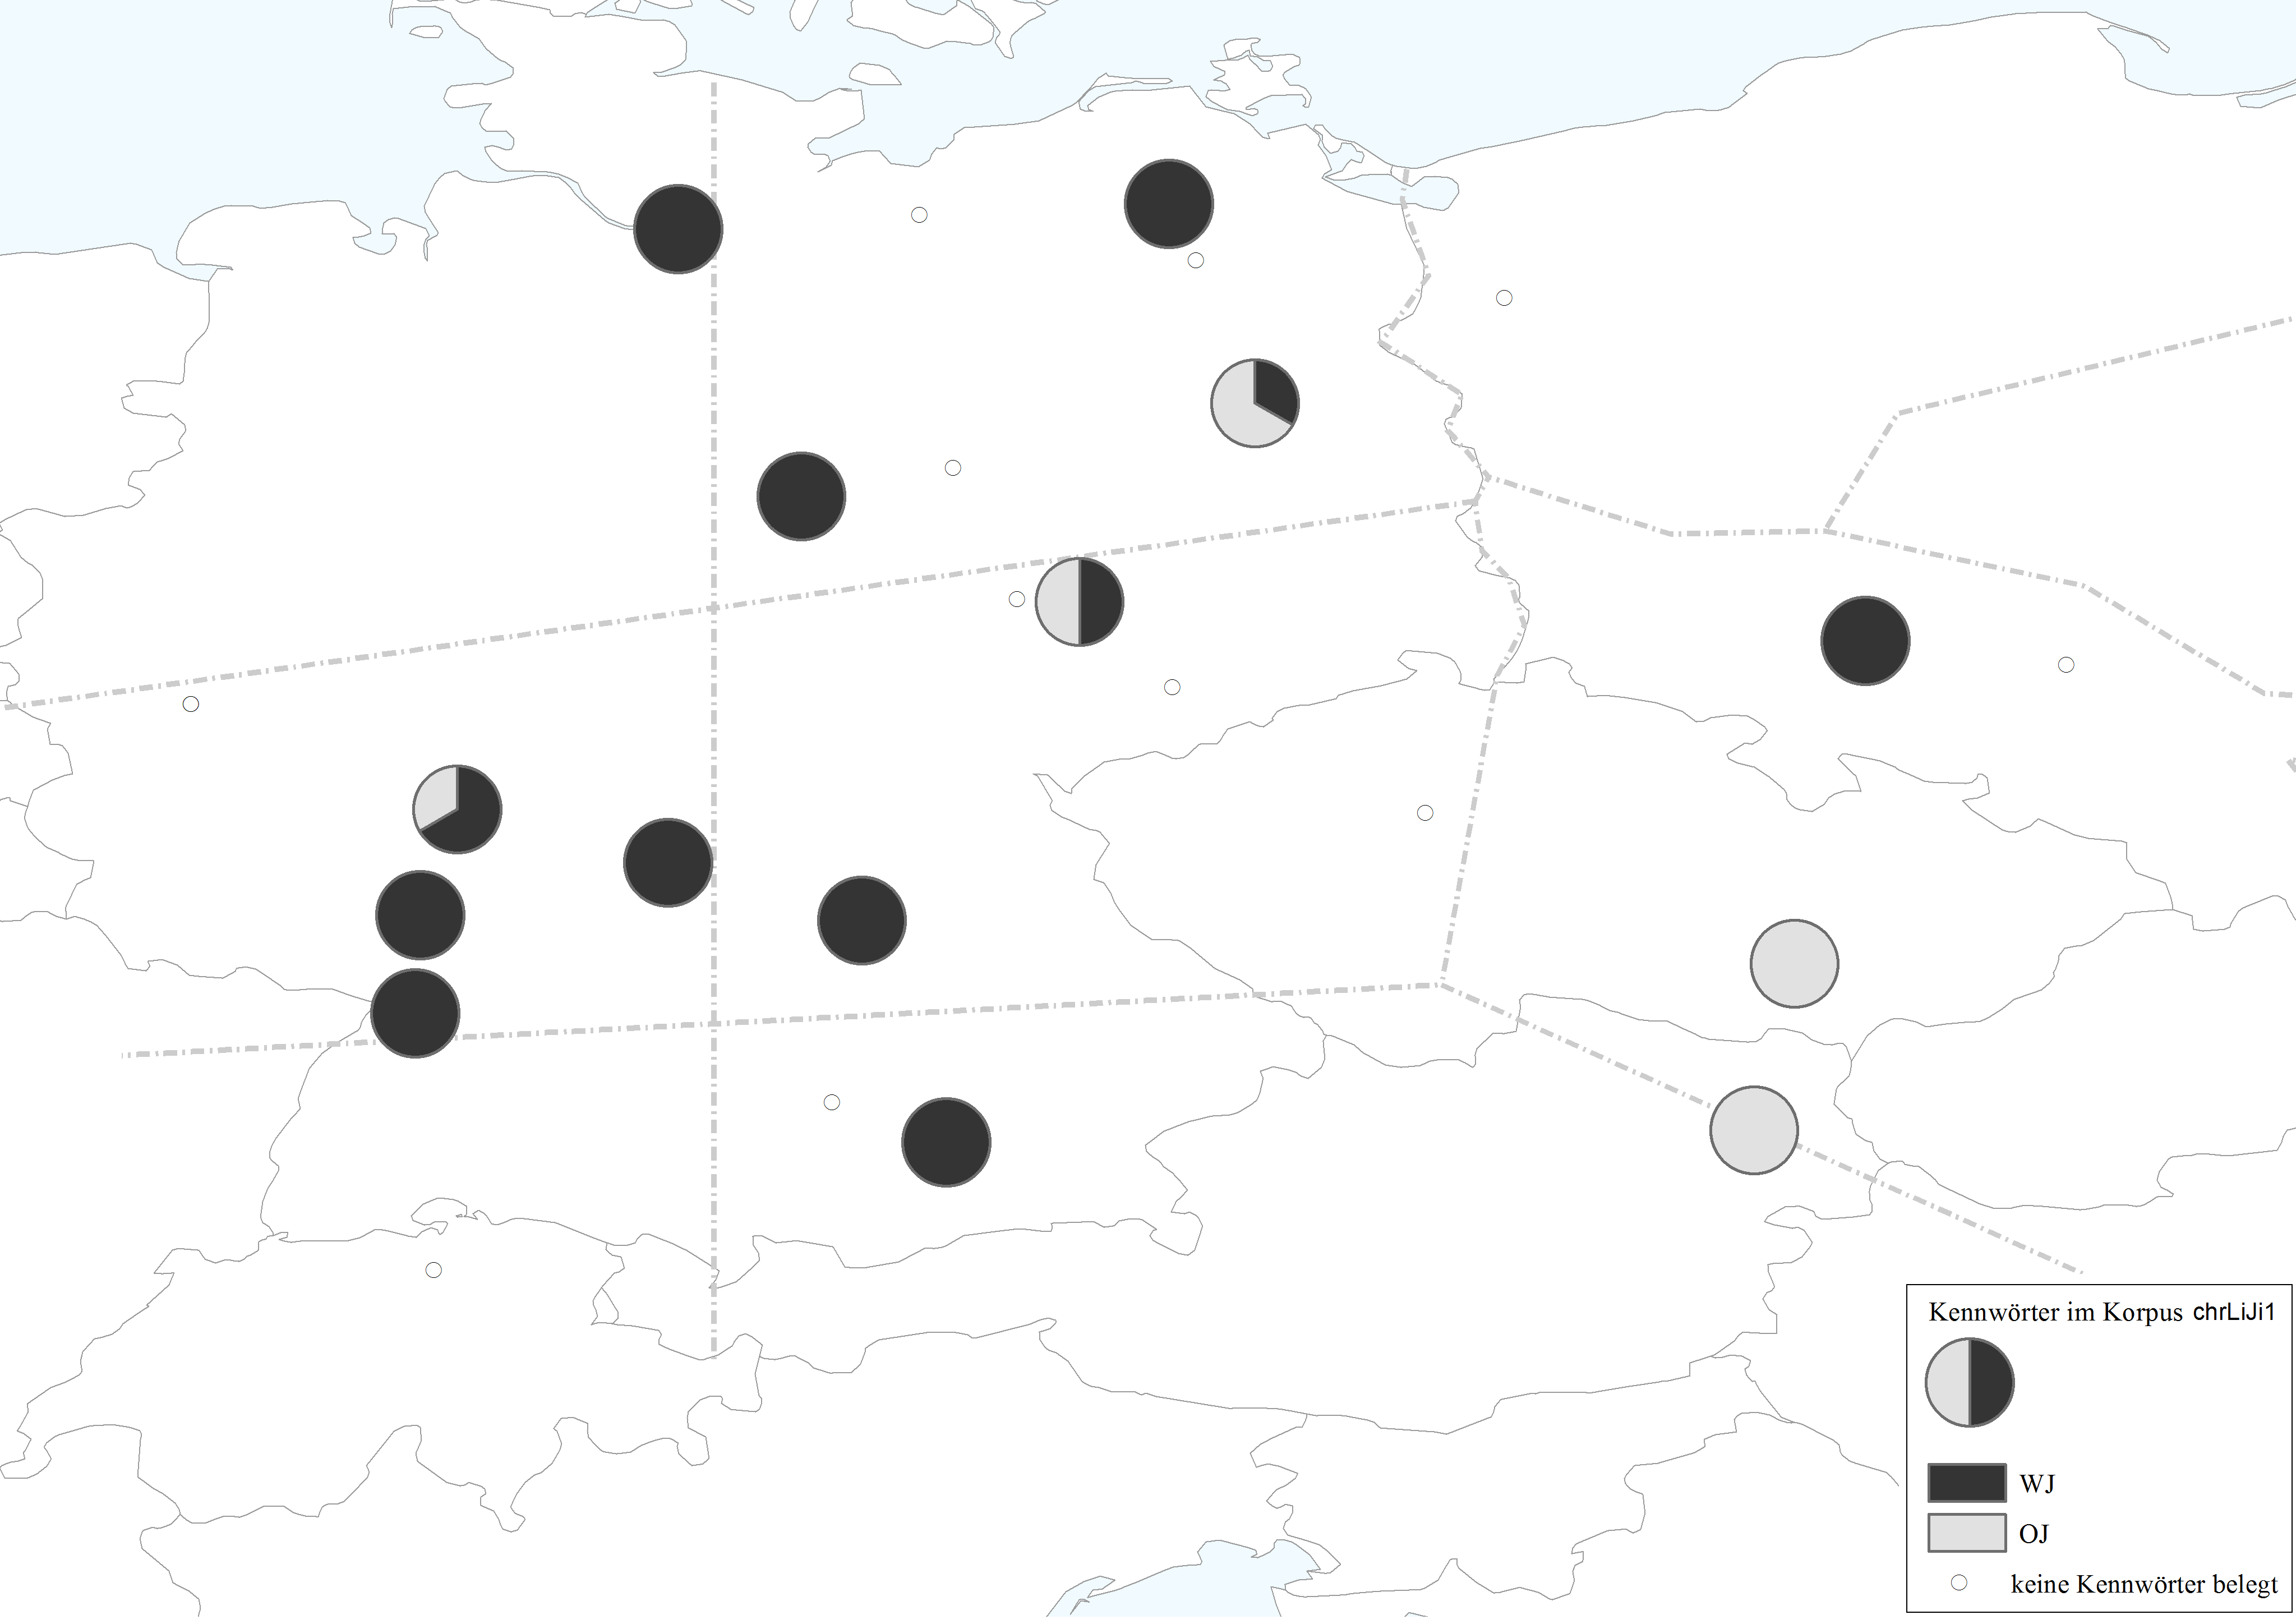
\includegraphics[width=\textwidth]{figures/kenn_diss.png}
\caption{\label{kennkarte} Kennwörter im \isi{Korpus} \hai{chrLiJi1}}
\end{figure} 
		


Eine der nur wenig bekannten innerwestjiddischen lexikalischen Variationen betrifft die Vokalisierung des \isi{Hebraismus}\il{hebräisch} \RL{שעה} \sem{Stunde}. Für das westliche \hai{{\SWJ}} ist die Form \textit{sche} belegt (\citealt[35]{GuggenheimGruenberg1976}\,\citealt[74]{Zivy1966}). Im \hai{{\NWJ}} hingegen findet sich die auch für das \hai{\OJ} übliche Form \textit{scho}. Wie genau diese binnenwestjiddische Isoglosse verläuft, ist leider nicht klar auszumachen, weil dieses Lexem für die relevanten Sprachräume des \hai{{\ZWJ}} und östl. \hai{{\SWJ}} nicht belegt ist. Im \hai{chrLiJi1} ist dieses Lexem in drei Fällen gegeben. In einer Quelle aus dem mitteldeutschen Raum findet sich sogar die aus dem Elsass und der Schweiz bekannte Form \textit{Scheh} \sem{Stunde} (\hai{OF} Frankfurt, 1711:\,1){;}\, als \textit{Scheih} findet sie sich in \hai{PG} (Speyer, 1835) (S.\,55) und die dem Ostjiddischen entsprechende Vokalisierung \textit{Schoh} ist in \hai{DG} (Wien, 1858) (S.\,14) belegt. In der Quelle \hai{PBreslau} des \hai{jüdLiJi1} findet sich ebenso die hier zu erwartende Form \textit{Schoh} (S.\,342).


Kennwörter, die lexikalische Unterschiede zwischen Ost- und \ili{Westjiddisch} markieren, sind im \hai{jüdLiJi1} nur wenige belegt. Westjiddische Lexeme treten keine auf, was auch mit Blick auf die geographische Lage der Quellen überraschend gewesen wäre. Statt dessen finden sich einige wenige ostjiddische Kennlexeme (Abbildung \ref{tblojkennjueliji1}).
 

\begin{table}
 
	\begin{tabular}{ll}
	\lsptoprule
\textbf{Kennwort} & \textbf{Beleg} \\ \midrule
 \textit{Tate} \sem{Vater} & \hai{GuS1} (3), \hai{GuS10} (9), \hai{PDebrecen} (7,\,14)\\
\textit{Mamme} \sem{Mutter} & \hai{GuS1} (3)\\ 
\lspbottomrule
\end{tabular}
			\caption{Ostjiddische Kennwörter im \hai{jüdLiJi1}} \label{tblojkennjueliji1}
\end{table}



      \section{Hebraismen}\label{hebrliji1}
%\noindent
Lexeme der \ili{hebräisch}-aramäischen\il{hebräisch} Komponente machen im (Surbtaler) Westjiddischen nach \citealt[45–49]
{GuggenheimGruenberg1976} einen Anteil von 2 bis 8\% aus. Im modernen Jiddisch sind es durchschnittlich 5\% des Wortschatzes \parencite[5f]{Timm2005}. Die tatsächliche Verwendung von Hebraismen ist jedoch stark von der Sprechsituation und Textsorte abhängig \parencite{Mark1954}. In beiden Varietäten machen Hebraismen jedoch im Allgemeinen nur einen äußerst geringen Anteil des Gesamtwortschatzes aus. 
 
Von 53 Quellen des \hai{chrLiJi1}-\isi{Korpus} setzen 44 Texte (83\%) Hebraismen zur Figurenmarkierung ein. Die Tokens variieren stark, was hauptsächlich der uneinheitlichen Textlänge geschuldet ist. Eine Frequenzuntersuchung gibt das \isi{Korpus} somit nicht her. Ich erlaube mir dennoch die sich rein auf den Leseeindruck stützende allgemeine Beobachtung, dass überwiegend Lexeme auftreten, welche Eingang in die deutsche Sprache gefunden haben (vgl. \citealt{Althaus2002,Althaus2004}). In sieben Quellen, in denen besonders viele und scheinbar der deutschsprachigen Mehrheit unbekannte (weil übersetzungbedürftige) Hebraismen eingesetzt werden, sind diese in Fußnoten oder einem Appendix übersetzt. Im überwiegenden Teil des \isi{Korpus} ist dies aber nicht der Fall und Hebraismen werden unübersetzt verwendet. Daraus lässt sich schließen, dass sie für Autor- wie Leserschaft als bekannt vorausgesetzt werden können.‏

  
Die rein qualitative Auswertung der Daten zeigt, dass bestimmte Types im intertextuellen Vergleich besonders häufig auftreten. Allen voran steht die Verwendung des Adjektivs \textit{meschugge} \sem{verrückt}, welches wir in 21 Quellen finden. Das entspricht 48\% der 44 Texte, in denen Hebraismen vorliegen. Ebenfalls relativ oft findet man die Lexeme \textit{Goi} \sem{Nichtjude} (in 12 Texten) und \textit{Schickse} \sem{Nichtjüdin} (in 10 Texten). Weitere 9\%–16\% der Quellen mit Hebraismen machen die in Tabelle \ref{tblhebrliji1} aufgeführten Types aus. 

\begin{table}
\centering
		\begin{tabularx}{\columnwidth}{lX}
	\lsptoprule
\textbf{Texte (\% von 44 Texten)} & \textbf{Type} \\ \midrule
 21 (48\%) & \textit{meschugge} \sem{verrückt}\\ %\midrule
12 (27\%) & \textit{Goi} \sem{Nichtjude} \\ %\midrule
 10 (23 \%) & \textit{Schickse} \sem{Nichtjüdin} \\ %\midrule
7 (16\%) &\textit{Dalles} \sem{Armut}, \textit{schmusen} \sem{sprechen} \\ %\midrule
6 (14\%) & \textit{dibbern} \sem{sprechen}, \textit{Reiwach}/\textit{Rewach} \sem{Gewinn}, \textit{koscher}/\textit{kauscher} \sem{(rituell) rein}\\ %\midrule
5 (11\%) & \textit{Massel} \sem{Glück}, \textit{Bonem}/\textit{Ponum} \sem{Gesicht}, \textit{acheln} \sem{essen}, \textit{Schaute}/\textit{Schoute} \sem{Narr}, \textit{Kapore} \sem{Verderben}, \sem{sterben}, \textit{Schama}/\textit{Schumme}/\textit{Schomme}  \sem{Seele}  \\ %\midrule
4 (9\%) &  \textit{Moos} \sem{Geld}, \textit{Schlamassel \sem{Unglück}}\\ \lspbottomrule

\end{tabularx}
			\caption{Häufige Hebraismen im \hai{chrLiJi1}} \label{tblhebrliji1}
\end{table}



Ein Großteil dieser Hebraismen sind Types, die in der deutschen Sprache eine hohe Tokenfrequenz haben. \textit{Verrückt} ist nach den Daten  \citeauthor{Ruoff1981}s (\citeyear[180]{Ruoff1981}) immerhin ein \isi{Adjektiv} der \hai{FK12} (\hai{FK7} innerhalb der Wortart). \textit{Sprechen} fällt in die \hai{FK9} der Verben, \textit{Glück} zählt zur \hai{FK10} (\hai{FK5} innerhalb der Wortart) und \textit{Gesicht} zur \hai{FK11} (\hai{FK6} innerhalb der Wortart) der Substantive \parencite[56, 55, 146]{Ruoff1981}. Die Grundfrequenz eines Lexems spielt also auch bei den Hebraismen eine Rolle.

Im \hai{jüdLiJi1} verwenden alle Texte der aufgenommenen \qu{Gedichte und Scherze in jüdischer Mundart} (\hai{GuS}) und alle Pamphlete, bis auf eine Ausnahme,\footnote{Die Ausnahme bildet \hai{PAlsleben}\,hier sind keine Hebraismen zu finden.} Hebraismen. Einige der im \hai{chrLiJi1} häufig auftretenden Types finden sich auch hier relativ oft (s. Tabelle \ref{tblhebrjuedliji1}), jedoch ist ein Vergleich der Korpora aufgrund des uneinheitlichen Textumfangs mit äußerster Vorsicht zu genießen. 

\begin{table}
\centering
	\begin{tabularx}{\textwidth}{lXX}\lsptoprule
\textbf{ Texte (\% von 10 Texten) } & \textbf{Type (Belegzahl \hai{GuS}:Pamphlete)} \\ \midrule
5 (50\%) & \textit{Goi} \sem{Nichtjude} (3:2)\\%\midrule
4 (40\%) & \textit{meschugge} \sem{verrückt} (2:2)\\%\midrule
3 (30\%) & \textit{koscher}/ \textit{kauscher} \sem{(rituell) rein} (2:1)\\%\midrule
2 (20 \%) & \textit{Schickse} \sem{Nichtjüdin} (2:0),  \textit{Kapore} \sem{Verderben}/ \textit{kapores} \sem{verderben}/ \sem{sterben} (1:1)\\%\midrule
1 (10\%) & \textit{schmusen} \sem{sprechen} (0:1), \textit{Ponim} \sem{Gesicht} (0:1), \textit{acheln} \sem{essen} (1:0)  \\
\lspbottomrule
\end{tabularx}
			\caption{Hebraismen im \hai{jüdLiJi1}} \label{tblhebrjuedliji1}
\end{table}




  \section{Interjektionen und psycho-ostensive Ausdrücke}\label{psycholiji1}
 %  %\noindent
Ein auffällig hoher Anteil der Texte arbeitet in der sprachlichen Markierung jüdischer Figuren mit Interjektionen und Phrasen des psycho-ostensiven Audrucks. 89\% (= 47 Texte) der Texte des \hai{chrLiJi1} \isi{Korpus} weisen diese Strategie auf. 

\subsection{Interjektionen}\label{interjektionen}
%  %\noindent
\largerpage
Ein interessantes Ergebnis ist, dass nicht viel Variation bei der Wahl der Interjektionen und Ausdrücke zu finden ist. Von orthographischen Alternativschreibungen abgesehen finden sich in den Texten die in Tabelle \ref{tblinterjektion} und exemplarisch in den Beispielen \ref{BSPinterjektion} aufgeführten Interjektionen. Allen voran steht die \isi{Interjektion} \textit{waih} \sem{wehe}, von der es mehrere Spielarten gibt (s. Tabelle \ref{tblwaih}). Gefolgt von der auch im Schriftdeutschen üblichen \isi{Interjektion} \sem{nun}. Die charakteristisch jiddischen Interjektionen \textit{oi} und \textit{nebbich} treten relativ selten auf (in insgesamt acht Texten vertreten). In einem Fall findet sich mit der eher aus dem oberdeutschen Raum bekannten \isi{Interjektion} \textit{mei} ein Einfluss der koterritorialen deutschen Dialekte (\ref{interjektmei}). Und auch die insgesamt sechs Belege für die \isi{Interjektion} \textit{ei} (\ref{interjektei}) kann Formen der Matrixsprache repräsentieren.

\begin{table}[t]
 
		\begin{tabular}{lccccccc}
	\lsptoprule
	\textbf{Interjektion} & \textit{waih} 	&   \textit{nu}, \textit{nü}  & \textit{ei}	&	\textit{oi} & \textit{nebbich}	& \textit{mei}	 \\ 
	& \sem{weh} & \sem{nun} & \sem{ei} & \sem{oh} & [unübersetzbar]\footnotemark & \sem{ja} \\ \midrule % horizontale Trennlinie
\textbf{Anzahl Texte} &	 36 & 25 & 6 & 3 & 3 & 1\\ \lspbottomrule
		 \end{tabular}
		 \caption{Interjektionen im \hai{chrLiJi1}}
		 \label{tblinterjektion}
		 \end{table}
		 
\footnotetext{Zu den verschiedenen Bedeutungen von \textit{nebbich} s. \citealt{Althaus1999}.}

\begin{table}[t]
 
		\begin{tabular}{lcccc}
			\lsptoprule
	\textbf{Interjektion} & \textit{au waih} & \textit{waih} 	&    \textit{waih geschrien}  & \textit{waih mer}	 \\ 
	& \sem{oh weh} & \sem{weh} & \sem{wehe geschrien} & \sem{wehe mir} \\ \midrule % horizontale Trennlinie
\textbf{Anzahl Texte} &	23 &  13 & 13 & 2 \\ \lspbottomrule
		 \end{tabular}
		 \caption{Varianten von \textit{waih} im \hai{chrLiJi1}}
		 \label{tblwaih}
		 \end{table}

 \eenumsentence{\label{BSPinterjektion}
\item \textit{O, waih mer, hot sich die ganze Welt} // \\
\textit{Auf einmol auf'n Kopf gestellt?!} (\hai{JP} Altona, 1867:\,15)\\\,%rs Absatz einfügen
	\sem{Oh weh mir, hat sich die ganze Welt auf einmal auf den Kopf gestellt?!}\label{interjektwai}

	\item \textit{Nü?! Worüm host Du mir gestaußen von Dir mit Antipäthie} (\hai{MV} Berlin, 1862:\,170)\\
	\sem{Na?! Warum hast du mich von dir mit Antipathie gestoßen}\label{interjektnu}


\item \textit{Ei hol dich der Teufel!} (\hai{AJ} Berlin, 1825:\,16)\label{interjektei}


\item \textit{Oi, a Broch!} (\hai{AK} Zürich, 1948:\,224)\\
	\sem{Oh, ein Fluch!}\label{interjektoi}
	
	\item \textit{Se wissen nichs, was is Nebbich? – Nebbich!} (\hai{GW} (n.a.,1900):\,4)\\
	\sem{Sie wissen nicht, was \textit{nebbich} ist? –\textit{Nebbich}!}\label{interjektnebbich}

	\item \textit{Mei, hab' ich doch oft die kleine Rosi auf meinen Armen getragen} (\hai{LP} Brünn, 1849:\,18)\\
	\sem{Ja, habe ich doch oft die kleine Rosi auf meinen Arm getragen}\label{interjektmei}

	
	}






 
In den Texten des \hai{jüdLiJi1} finden sich dieselben Interjektionen wie im \hai{chrLiJi1} (s. Tabelle \ref{tblwaihjüdliji}). In vier Quellen der \hai{GuS} findet sich \textit{nu}, in jeweils einer \textit{au mir},  \textit{ei weih} und  \textit{weih}. Die Pamphlete verwenden in jeweils zwei Texten \textit{weih geschriehn} und \textit{nu}. Es liegt damit, abgesehen von der \isi{Orthographie} des Diphthongs in \textit{waih} vs. \textit{weih}, kein Unterschied bei der Wahl der Interjektionen im Vergleich zu den Quellen des \hai{chrLiJi1} vor. 


\begin{table}
	
		\begin{tabular}{lccccc}
		\lsptoprule
	\textbf{Interjektion} & \textit{nu} & \textit{weih geschriehn}  & \textit{au mir} 	&    \textit{ei weih}  & \textit{weih}	 \\ 
	& \sem{nun} & \sem{wehe geschrien}& \sem{oh mir} & \sem{oh weh} & \sem{weh} \\ \midrule % horizontale Trennlinie
\textbf{Anzahl Texte} &	6 &  2 & 1 & 1 & 1 \\ \lspbottomrule
		 \end{tabular}
		 \caption{Interjektionen im \hai{jüdLiJi1}}
		 \label{tblwaihjüdliji}
		 \end{table}



   \subsection{Psycho-ostensive Ausdrücke}\label{psych}
  %  %\noindent
  Die in Unterabschnitt \ref{interjektionen} vorgestellten Interjektionen dienen vorrangig dem Ausdruck eines seelischen Zustandes des Sprechers. Darüber hinaus finden sich in den Korpora Phrasen des psycho-ostensiven Ausdrucks.  \textcite{Matisoff2000} fasst am Beispiel des modernen Ostjiddischen zwölf mögliche Subtypen dieser Ausdrücke zusammen, an denen sich die Analyse der Korpusdaten orientiert. Inwiefern das Jiddische einen besonderen Reichtum solcher Ausdrücke hat, wurde bislang noch nicht auf empirischer Grundlage bestätigt, es scheint aber im Allgemeinen als \textit{Mythos} dem Jiddischen anzuhängen (vgl. \citealt[4]{Matisoff2000}). 
  
In den Texten des \hai{chrLiJi1} finden \,%rs Pluralbezug
sich die in Tabelle \ref{tblpsych}  aufgeführten Typen, die hier mit allen erhobenen Belegen versehen sind. Es überwiegen senderbezogene Äußerungen gegenüber empfängerbezogenen, was sicherlich auf die literarische Rolle der jeweiligen Judenfiguren als weitestgehend isolierte Gegenspieler zurückzuführen ist. 

  \begin{table}[t]
%\centering
		\begin{tabularx}{\columnwidth}{lX}
		\lsptoprule
	Typ & Beleg	 \\ \midrule % horizontale Trennlinie
	

allo-bono-petitive & \textit{daß sie sollen hundert Johr leben!} (\hai{DW}:\,69){;}\,  \textit{Gott behüt se} (\hai{FE}:\,16){;}\, \isi{Eigennamen} \& Verwandtschaftsbezeichnungen mit \textit{-leben}:  \textit{Bohlmannleben} (\hai{DP}:\,5), \textit{Mosisleben} (\hai{DP}:\,15), \textit{Kinderleben} (\hai{JP}:\,5, 19),  \textit{Sorcheleben}  (\hai{JP}:\,17R),  \textit{Memmeleben} (\hai{JP}:\,22R),  \textit{Etteleben} (\hai{JP}:\,52),  \textit{Doktorleben} (\hai{SS}:\,12),  \textit{Inspektorleben} (\hai{SS}:\,13),  \textit{Herrgottleben} (\hai{SS}:\,25),  \textit{Rebbeleben} (\hai{SS}:\,26{;}\, \hai{GW}:\,19), \textit{Rüfkeleben} (\hai{GW}:\,10), \textit{Mutterleben} (\hai{GW}:\,10), \textit{Meierleben} (\hai{GW}:\,12), \textit{Narreleben} (\hai{GW}:\,12), \textit{Direktorleb'm} (\hai{GW}:\,12), \textit{Schmulleben} (\hai{GW}:\,14), \textit{Tateleben} (\hai{GW}:\,15), \textit{Jankefleben} (\hai{GW}:\,32). \\
% \tablevspace
auto-bono-petitive & \textit{soll ich leben} (\hai{JP}:\,24). \\
% \tablevspace
auto-malo-fugitive & \textit{Gott soll hüten} (\hai{SS}:\,19), \textit{Gott behit} (\hai{AT}:\,88, 89, 90, 109){;}\, \textit{Gott soll mich bewohre} (FE:\,\hai{14}), \textit{Gott soll me schamer seyn} (\hai{FE}:\,56), \textit{Soll mir Gott helfen} (\hai{FS}:\,40, 42), \textit{Gott soll schützen!} (\hai{AJ}:\,1, 2, 6, 10), \textit{Gott soll mir helfen!} (\hai{AJ}:\,1), \textit{Gott soll mer helfen} (\hai{PF}:\,9, 21), \textit{Soll mir Gott helfen} (\hai{PM}:\,212, 218).\\ 
% \tablevspace
auto-malo-recognitive & \textit{waih mir} (\hai{JP}:\,15, 42), \textit{Wey mir!} (\hai{AO}:\,85){;}\, \textit{nebbisch} (\hai{SS}:\,13), \textit{nebech} (\hai{DG}:\,6), \textit{nebbich} (\hai{GW}:\,4,5,10){;}\, \textit{was thu ich damit!} (\hai{NW}:\,11), \textit{was thu’ ich damit!} (\hai{EV}:\,279), \textit{Was duh ich domit?} (\hai{TH}:\,98), \textit{was thut mer damit?} (\hai{EJ}:\,38){;}\, \textit{mahn Seel} (\hai{SV}:\,4), \textit{meine Schama} (\hai{LP}:\,41), \textit{meine Schumme} (\hai{OF}:\,2), \textit{man'neschommæ} (\hai{LR}:\,6). \\
% \tablevspace
auto-bono-recognitive & \textit{Gotts Wunder} (\hai{PF}:\,12, 17, 19), \textit{Gottes Wunder} (\hai{LP}:\,14), \textit{Gotteswunder} (\hai{LP}:\,15).
 \\\lspbottomrule

		 \end{tabularx} 
		 \caption{Psycho-ostensive Ausdrücke im \hai{chrLiJi1}}
		 \label{tblpsych}
		 \end{table}   
  % \clearpage
   
   
   
 Das \hai{jüdLiJi1} zeigt deutlich weniger solcher Ausdrücke. Lediglich in drei Belegen liegen auto-malo-fugitive (\ref{fugitivjuedliji1}) und auto-bono-petitive Ausdrücke (\ref{petitivejuedliji1}) aus der Quelle \hai{PBerlin1} vor:
 \eenumsentence{
	\item \textit{soll mer Gott helfen} \\
	\sem{soll mir Gott helfen} (\hai{PBerlin1}:\,2, 6)\label{fugitivjuedliji1}

	\item \textit{soll ich leben} (\hai{PBerlin1}:\,4)\label{petitivejuedliji1}

	
	}
     
 Die geringe Belegzahl an psycho-ostensiven Ausdrücken im \isi{Korpus} des \hai{jüdLiJi1} ist jedoch kein Indiz dafür, dass solche Ausdrücke im gesprochenen Westjiddischen kaum verbreitet waren. Zumindest das westjiddische Theaterstück \quji{\RL{דיע ה{א\makebox(-1.25,-1.25)[r]{\libertineGlyph{uni05B8}}}כצייט צו גר{א\makebox(-1.25,-1.25)[r]{\libertineGlyph{uni05B8}}}בסד{א\makebox(-1.25,-1.25)[r]{\libertineGlyph{uni05B8}}}רף}} [\qu{Die Hochzeit zu Grobsdorf}] (1822) gebraucht solche Ausdrücke besonders häufig, wie die Beispiele in (\ref{psychgrob}) zeigen.
 \eenumsentence{\label{psychgrob} \,%rs Absätze zwischen Zitierform und Übersetzung 
 	\item  \RL{איבער הונדערט י{א\makebox(-1.25,-1.25)[r]{\libertineGlyph{uni05B8}}}הר} \\
    \sem{über hundert Jahre (soll er alt werden)} allo-bono-petitive\\
    (\qu{Die Hochzeit zu Grobsdorf} 1822:\,13)\footnote{Die Seitenangaben folgen der Seitennummerierung der Handschrift aus der Max Weinreich Collection (Sig.: RG 584), auf welchem die Jahresangabe \qu{1822} zu finden ist.} 
    
	\item \RL{נ{א\makebox(-1.25,-1.25)[r]{\libertineGlyph{uni05B8}}}ך הונדערט קינדער}\\
    \sem{noch hundert Kinder (soll ich bekommen)} auto-bono-petitive\\
    (\qu{Die Hochzeit zu Grobsdorf} 1822:\,14) 
 
 	\item \RL{מיינע שמה}\\ 
    \sem{meine Seele} auto-malo-recognitive\\
    (\qu{Die Hochzeit zu Grobsdorf} 1822:\,u.\,a.\, 6,16,20,21,22) 
 }

Allgemein lässt sich festhalten, dass jüdische Figuren in allen Stadien des \hai{{\LiJi}} über besondere Ausdrücke entwickelt werden, die den psychischen Zustand des Sprechers ausdrücken.
Tatsächlich sind solche Ausdrücke für die (west-)jiddische Sprachrealität dokumentiert vgl. Bsp. in (\ref{psychgrob}). Ob sie jedoch mit der \isi{Frequenz}, wie wir es im \hai{chrLiJi1} finden, auch in der gesprochenen Sprache verwendet wurden, muss offen bleiben. Der hohe Gebrauch von Interjektionen im \hai{chrLiJi1} spricht dafür, dass diese, allen voran Variationen mit \textit{waih}, auch im literarischen Diskurs als besondere Kennzeichen jüdischer Figuren dienen.

\section{Gallizismen}\label{galliliji1}
%\noindent
Im Bereich der Lexik sei noch ein letztes Phänomen näher beleuchtet. Stark verbunden mit dem \qu{Juden-Französisch-Deutsch} \parencite[175]{Gelber1986} (s. Unterabschnitt \ref{assimiliert}) ist die Verwendung von Gallizismen im \hai{chrLiJi1}.
Die in (\ref{bspgall}) aufgeführten Belege zeigen, dass keine bestimmten Lexeme besonders häufig auftreten, wie es im Fall der Interjektionen und psycho-ostensiven Ausdrücken gegeben ist (Abschnitt \ref{psycholiji1}). Unter den Gallizismen sind einige, die bereits in das System der Matrixsprache integriert sind z.\,B.\, (\ref{mammsellchen}), (\ref{arretueren}) und damit nicht zwangsläufig als Produkte der sprachlichen Manipulation gewertet werden müssen. 

\eenumsentence{

	\item\textit{l’age} \sem{Alter} (\hai{BW} Leipzig, 1826:\,101)
\item\textit{par tout} \sem{um jeden Preis}  (\hai{PL} Mannheim, 1780:\,41)
\item \textit{Cavaliers} \sem{Kavalliere} (\hai{DW} Wien, 1773:\,71)
\item \textit{Dames} \sem{Frauen} (\hai{DW} Wien, 1773:\,71{;}\, \hai{PA} Frankfurt, 1834:\,5)   
\item\textit{Trän} \sem{Zug} (\hai{PM} Magdeburg, 1792:\,219)
\item\textit{Plaisir} \sem{Freuden} (\hai{FS} Schwerin, 1805:\,41)
\item \textit{wollt ich gern seyn content} \sem{ich möchte zufrieden sein} (\hai{FS} Schwerin, 1805:\,42)
\item\textit{Malleur} \sem{Unglück} (\hai{TH} Merseburg, 1820:\,115){;}\, \textit{malheur} \sem{Unglück} (\hai{AD} Leipzig, 1846:\,135)
\item \textit{Mamsellchen} \sem{Fräulein} (\hai{TH} Merseburg, 1820:\,122)\label{mammsellchen}
\item \textit{foi de parol} \sem{Wort des Glaubens} (\hai{AJ} Berlin, 1825:\,2)   
\item\textit{arretüren} \sem{festnehmen} (\hai{AB} Hamburg, 1850:\,47)\label{arretueren}
\item\textit{fête} \sem{Fest} (\hai{AD} Leipzig, 1846:\,136)
  }\label{bspgall}

Die Markierung funktioniert nicht über die Lexeme selbst, sondern allein über die Wahl der Sprache. Dabei treten in den meisten Fällen nur einzelne Lexeme innerhalb des \hai{{\LiJi}} auf, keine Sätze oder Phrasen. Einzige Ausnahme ist dabei Sessas Stück \hai{JK} (Breslau, 1810), in dem die jüdische Hauptfigur mit einem französischen Soldat \ili{französisch}, bzw. \qu{Juden-Französisch-Deutsch} \parencite[175]{Gelber1986}, spricht: \\

\eenumsentence{

	\item\textit{Qui, qui, nous sommez des pauvres Juifs, amix von där graußen Nation.}\\
	 (\hai{JK} Breslau, 1810:\,37–38)\\
	\sem{Wer, wer{;}\, wir sind arme Juden, Freunde von der großen Nation.}
}\label{galljk}
   
Die elf\, Texte, in denen wir Gallizismen finden, streuen diachron interessant. Nach 1850 bricht diese Strategie der Figurencharakterisierung ab (s. Abbildung \ref{gall}). 

%%%Gallizismen%\begin{flushleft}	
\begin{figure}
	\begin{tikzpicture}
		\begin{axis}[only marks, width=0.82\textwidth,height=0.2\textheight,
		legend style={at={(1,1)},xshift=+0.2cm, yshift=-0.25cm,anchor=north west,nodes=left},
			%title={Funktionstypen des sp\"aten Westjiddisch},
			xtick={1700, 1725, 1750, 1775, 1800, 1825, 1850, 1875, 1900, 1925, 1950, 1975}, ytick=\empty,
			x tick label style={/pgf/number format/1000 sep=}, 
			y tick label style={/pgf/number format/1000 sep=},
			%extra y ticks={456.1, 1022.4},
			%extra y tick labels={{456,1},{1022,4}},
			extra y tick style={grid=major,
				tick label style={, ,}},
				ymin=0.7,
				ymax=2.5,
			ylabel={Phänomenbelege},
			enlarge x limits=0.03]	
	%TT problem?
			
		\addplot [mark=*, black] table [x=jahr, y=gall] {figures/gall.txt};
	\addplot [mark=o, black] table [x=jahr, y=no] {figures/gall_no.txt};

			% Andere Formen a={mark=square*,blue},% b={mark=triangle*,red},% c={mark=o,draw=black}}
						\legend{Gallizismen, übrige Quellen} %macht Legende
		\end{axis}
	\end{tikzpicture}
	\caption{Gallizismen im \hai{chrLiJi1}}
	\label{gall}	
\end{figure}
 %TT no-Belege aufführen!

   
Dieses Phänomen ist auf das \hai{chrLiJi1} beschränkt. Im \hai{jüdLiJi1} spielen Gallizismen keine Rolle. Es ist eindeutig ein pejoratives Element des \hai{chrLiJi1} und hat keine Entsprechung in autochthonen Quellen des Westjiddischen. Gallizismen tragen zum einen die Funktion, den Multilingualismus und damit unter pejorativer Verwendung den Mythos eines \textit{globalen jüdischen Verschwörungsnetzwerks} zu vermitteln. Zum anderen aber verbindet die gezielte Verwendung des Französischen das Feindbild \textit{Franzose} mit dem Feindbild \textit{Jude} (vgl. Abschnitt \ref{assimiliert}, S.\, \pageref{judenfranzoesischdeutscherstmals}).  
\chapter{Phonologische Markierungen}\label{phonologie}
 %\noindent
Graphem und \isi{Phonem} sind nicht \isi{ikonisch} aufeinander bezogen,\footnote{Abgesehen vom koreanischen Hangul, wo zumindest ansatzweise Artikulationsort und Zungenposition eines Lautes im Graphem dargestellt sind \parencite[32]{Sampson1985}.} aber Grapheme haben eine Verweisfunktion auf Phoneme. Die Autoren des \hai{{\LiJi}} arbeiten gezielt mit der Erwartungshaltung des Lesers an ein standarddeutsches Schriftsystem, deren phonematische Äquivalenzen jeder Alphabetisierte kennt. Im \hai{{\LiJi}} werden Abweichungen vom Standardsystem eingesetzt, um eine sich vom Deutschen unterscheidende phonetische Realisierung zu evozieren. Die Analyse der sich hinter den abweichenden Graphemen verbergenden Phoneme wird dabei dem Leser selbst überlassen, der ohne weiteres von erlernten Orthographieregeln abweichen kann. Die nachfolgenden Analysen müssen, da es sich um ein schriftsprachliches \isi{Korpus} handelt, ebenso von der Graphemebene auf die Phonemebene abstrahieren. Rückschlüsse auf phonetische Einheiten sind dabei jedoch mit Vorsicht zu ziehen. Es scheint im \isi{Vokalismus} ergiebiger, sich auf historische Vokale des Mittelhochdeutschen und Protojiddischen zu beziehen;\, im \isi{Konsonantismus} hingegen, wo schriftliche Daten besonders problematisch sind, muss vorsichtshalber rein graphematisch im Vergleich zum Standarddeutschen gearbeitet werden.
 
 Es wird im Folgenden eine Auswahl der im \hai{{\LiJi}} am häufigsten auftretenden phonologischen Phänomene einzeln und unabhängig von der Lexemebene betreffs ihrer Verteilung in den verschiedenen Korpora, im geographischen Raum und über die gegebene Zeitspanne hinweg analysiert. Da Dramen deutlich überrepräsentiert sind, ergibt eine Analyse der Verteilung eines Phänomens in Abhängigkeit von der Textsorte wenig Sinn. Bevor jedoch die Analysen der Einzelphänomene dargestellt werden, soll zunächst geklärt werden, wie lexemgebunden die phonologischen Manipulationen sind und ob vorwiegend Lexeme mit generell hoher \isi{Frequenz} (nach \citealt{Ruoff1981}) phonologisch markiert werden oder ob Lexeme im \isi{Korpus} hochfrequent sind, die in der gesprochenen Sprache eher niedrigfrequent sind, und so in der Funktion von Kennwörtern für jüdische Sprache fungieren. Denn nur ein Ergebnis zugunsten der lexematischen Ungebundenheit phonologischer Phänomene erlaubt es, bei den Einzelanalysen von der Lexemebene auf die Phonemebene zu abstrahieren.
 %\clearpage

 
Um offen zu legen, nach welchen Kriterien bestimmte Phänomene in die Einzelanalysen aufgenommen wurden und andere nicht, wird in Abschnitt \ref{phonalles} eine Übersicht zu den häufigsten im \hai{{\LiJi}} anzutreffenden phonologischen Manipulationen gegeben. Dies ermöglicht auch schon eine erste allgemeine Auswertung der Manipulationsstrategien. Lediglich vereinzelt auftretende Phänomene, zumeist \quein{Fehler} oder Hyperkorrekturen werden nicht näher analysiert, sondern als \quein{Störgeräusch} herausgefiltert, da es in dieser Untersuchung darum geht, erkannte und angewandte Regeln und deren diachrone Entwicklungen aufzudecken und darzustellen.   
 
 Die ersten Überlegungen zu einem protojiddischen Vokalsystem stammen von \cite[251–254]{WeinreichU1958}; aber erst \cite{Weinreich1960} stellt von den Überlegungen seines Sohnes ausgehend ein System vor, welches er später nur leicht korrigiert \parencite[658–718]{Weinreich1973}. Marvin Herzogs Ansatz (\citeyear{Herzog1965}) wiederum erweitert \citeauthor{Weinreich1960}s Modell von \citeyear{Weinreich1960};der grundlegende Unterschied zwischen \citeauthor{Weinreich1960}s und \citeauthor{Herzog1965}s Modell besteht in einem anderen Siglen-System, welches eine größere Distanz zu den {\urj} Rekonstruktionen aufbaut und damit die Abstraktion, die ein rekonstruiertes Protosystem mit sich bringt, unterstreicht. Allein aus diesem Grund folgen die phonologischen Analysen dieser Arbeit dem Modell von  \cite[161–205]{Herzog1965}. Die einzelnen Abschnitte nennen neben den Herzogschen Siglen immer auch die jeweilige mittelhochdeutsche Entsprechung und die Sigle \citeauthor{Weinreich1973}s  (\citealt[658–718]{Weinreich1973} = \hai{LCAAJ}).\footnote{Eine phonetische Annäherung an ein protojiddisches Vokalsystem, auf die die vorliegende Arbeit keinen Bezug nimmt, findet sich in \cite{Jacobs1990}. Eine Zusammenschau der verschiedenen Modelle findet sich in \cite[insbes. S.\, 86 Tabelle 18]{Beider2010}.} Das protojiddische Vokalsystem, wie es diese Arbeit verwendet, ist in Tabelle \ref{vokalsystem} dargestellt. Alle protojiddischen Vokalsysteme setzen für die germanische Komponente des Jiddischen das mittelhochdeutsche System voraus. Doch wie die Zusammenschau in Tabelle \ref{vokalsystem} gut verdeutlicht, gehen die meisten Protovokale bereits von Zusammenfällen aus mittelhochdeutschen Vokalen aus. Das Protojiddische setzt so überwiegend Formen voraus, die sich zwar aus dem modernen \hai{{\OJ}}  ableiten lassen, jedoch historisch eher jüngere Sprachstadien des Mitteljiddischen repräsentieren, kaum aber die Situation im Altjiddischen bzw. einem älteren protojiddischen System entsprechen können.\footnote{So sind in etwa die Resultate der sog. \quein{neuhochdeutschen Diphthongierung} von {\mhd} \textit{î}, \textit{iu}, \textit{û} oder auch der \quein{neuhochdeutschen Monophthongierung}
 von {\mhd} \textit{ie}, \textit{ue}, \textit{uo} fester Bestandteil der jiddischen Protovokale (vgl.\, \citealt[§L17]{Paul2007}).} Damit ist es m.\,E. anzuzweifeln, dass das protojiddische System einen jiddischen \textit{Urzustand} beschreibt. So ist es sinnvoll, das (normalisierte) mittelhochdeutsche Vokalsystem als Referenzsystem mit anzuführen.
 
 Die nachfolgende Analyse wird den \isi{Vokalismus} von Hebraismen nicht näher analysieren, da diese für die emulierende \isi{Imitation} kaum eine Rolle spielen. So gesehen könnte zu Gunsten des Mittelhochdeutschen als Ausgangssystem auf das protojiddische System verzichtet werden. Aus dem Wunsch, die Distanz zwischen historischem und rekonstruiertem Laut zu wahren und aus Respekt vor der jiddistischen Tradition wurde das mittelhochdeutsche System als primäre terminologische Ausgangsbasis jedoch ausgeschlossen;\, das heißt nicht, dass auf dieses gänzlich verzichtet wurde. Insbesondere, da wir es hier mit der Manipulation germanischer Lexeme zu tun haben, werden das Mittelhochdeutsche und auch die deutschen Dialekte eine besondere Rolle spielen.

 \begin{table}
 \begin{tabularx}{\textwidth}{p{1cm}p{2cm}p{1.7cm}p{1.7cm}Q}
				\lsptoprule
	\textbf{Proto-vokal} & \textbf{Herzog} \textbf{(1965)} & \textbf{Weinreich} \textbf{(1960)} & \textbf{{\mhd}} \textbf{Entsprechung} & \textbf{Beispiel} \textbf{mod.} \textbf{\hai{{\OJ}} (\textbf{Weinreich 2008})} \\ \midrule 

*\textit{a} &\hai{V11} & \hai{A\textsubscript{1}} & \textit{a} & \RL{גא\makebox(-1.5,-7.5)[r]{\libertineGlyph{uni207B}}סט} \textit{gast} \sem{Gast} \\

*\textit{\textopeno\textlengthmark} &\hai{V12}, \hai{V13}\textsuperscript{\dag}
& \hai{A\textsubscript{2}}, \hai{A\textsubscript{3}} & \textit{â}, \textit{a} & \RL{י{א\makebox(-1.25,-1.25)[r]{\libertineGlyph{uni05B8}}}ר} \textit{jor} \sem{Jahr}, \RL{ז{א\makebox(-1.25,-1.25)[r]{\libertineGlyph{uni05B8}}}גן} \textit{zogn} \sem{sagen} \\


*\textit{\textepsilon\textlengthmark} &\hai{V21} & \hai{E\textsubscript{1}} & \textit{ë} & \RL{געלט} \textit{gelt} \sem{Geld} \\	

*\textit{\textepsilon} & \hai{V25}\textsuperscript{{\dag}}  & \hai{E\textsubscript{5}} & \textit{ê}, \textit{ë} & \RL{שעמען} \textit{shemen} \sem{schämen}, \RL{מעל} \textit{mel} \sem{Mehl}, \RL{לעבן} \textit{lebn} \sem{leben} \\	

*\textit{e\textlengthmark} &\hai{V22}, \hai{V23}\textsuperscript{{\dag}}  & \hai{E\textsubscript{2}}, \hai{E\textsubscript{3}} & \textit{ê}, \textit{ë}, \textit{œ}, \textit{öu} &  \RL{שניי} \textit{shney} \sem{Schnee}, \RL{גיין} \textit{geyn} \sem{gehen}, \RL{נייטיק} \textit{neytik} \sem{nötig}, \RL{הע{פ\makebox(-0.8,9)[r]{\libertineGlyph{uni207B}}}לעך} \textit{heflekh} \sem{höflich}, \RL{{פ\makebox(-0.8,9)[r]{\libertineGlyph{uni207B}}}רייד} \textit{freyd} \sem{Freude}  \\ 

*\textit{\textschwa i\textlengthmark} & \hai{V24} & \hai{E\textsubscript{4}} & \textit{ei} & \RL{{פ\makebox(-0.8,9)[r]{\libertineGlyph{uni207B}}}לייש} \textit{fleysh} \sem{Fleisch} \\	
	

 *\textit{i} &\hai{V31} & \hai{I\textsubscript{1}} & \textit{i}, \textit{ü}  & \RL{שיף} \textit{shif} \sem{Schiff}, \RL{דין} \textit{din} \sem{dünn} \\

 *\textit{i\textlengthmark} &\hai{V32}, \hai{V33}\textsuperscript{{\dag}}  & \hai{I\textsubscript{2}}, \hai{I\textsubscript{3}} & \textit{i}, \textit{üe} & \RL{בריוו} \textit{briv} \sem{Brief}, \RL{גרין} \textit{grin} \sem{grün} \\	

*\textit{\textschwa i\textlengthmark} &\hai{V34} & \hai{I\textsubscript{4}} & \textit{î}, \textit{iu} & \RL{צ{יי}\makebox(-1.5,-3.5)[r]{\libertineGlyph{uni207B}}ט} \textit{tsayt } \sem{Zeit}, \RL{ה{יי}\makebox(-1.5,-3.5)[r]{\libertineGlyph{uni207B}}נט} \textit{haynt} \sem{heute}\\

*\textit{\textopeno} &\hai{V41} & \hai{O\textsubscript{1}} & \textit{o} & \RL{װ{א\makebox(-1.25,-1.25)[r]{\libertineGlyph{uni05B8}}}ך} \textit{vokh} \sem{Woche} \\

*\textit{o\textlengthmark} &\hai{V42}, \hai{V43}\textsuperscript{{\dag}} & \hai{O\textsubscript{2}}, \hai{O\textsubscript{3}} & \textit{ô} & \RL{ברויט} \textit{broyt} \sem{Brot} \\

*\textit{\textopeno u\textlengthmark} &\hai{V44} & \hai{O\textsubscript{4}} & \textit{ou} & \RL{אויג} \textit{oyg} \sem{Auge} \\


*\textit{u} &\hai{V51} & \hai{U\textsubscript{1}} & \textit{u} & \RL{זון} \textit{zun} \sem{Sonne} \\

*\textit{\=u\textlengthmark} &\hai{V52}, \hai{V53}\textsuperscript{{\dag}}  & \hai{U\textsubscript{2}}, \hai{U\textsubscript{3}} & \textit{uo} & \RL{ברודער} \textit{bruder} \sem{Bruder}, \RL{בוך} \textit{bukh} \sem{Buch} \\  


*\textit{\textschwa u\textlengthmark} &\hai{V54} & \hai{U\textsubscript{4}} & \textit{û} & \RL{הויז} \textit{hoyz} \sem{Haus} \\  
\lspbottomrule
	  \end{tabularx}  
 \caption{Das protojiddische Vokalsystem nach dem Modell \citeauthor{Herzog1965}s (\citeyear[161–205]{Herzog1965}) ergänzt um die mittelhochdeutschen und Weinreich'schen Entsprechungen}
\label{vokalsystem}	  
%%% \rule{0.3\textwidth}{0.4pt} \\

\parbox{.9\textwidth}{{\textsuperscript{\dag}\footnotesize Alle Vokale mit dem Zahlenwert \quein{3} und \quein{5} sind ursprünglich kurz, wurden aber später inbesondere durch die Dehnung in offener Tonsilbe oder allomorphische Alternanzen gedehnt (vgl.\, \citealt[1024]{Katz1983}).} 
}
%tblformatOK  Anmerkung verrutscht hier;\, Lösung?! Soll unter  Tabelle stehen
\end{table} 

\section{Frequenzen phonologisch manipulierter Lemmata}

%\noindent 
Die Tabelle \qu{\isi{Frequenz} phonologisch markierter Types im \hai{{\LiJieins}}} im Appendix (ab S.\, \pageref{tblFKphon}) führt die häufigsten verwendeten Lemmata auf, die im \isi{Korpus} phonologisch modifiziert wurden, und stellt sie den aus den Daten \citeauthor{Ruoff1981}s (\citeyear{Ruoff1981}) gewonnenen \hai{FK}n und den \hai{FK}n des \hai{DeReKo} (2012) gegenüber.\footnote{Es wurden Types nach einer maximalen Häufigkeit von \( \geq4 \)  Texten aufgenommen.} Wir sehen, dass hochfrequente Types auch besonders häufig in mehreren Texten manipuliert werden. Allen voran stehen die Lemmata \sem{haben} (52 Texte), \sem{ein} (51 Texte), \sem{kein} (50 Texte), \sem{groß} (46 Texte), \sem{auch} (45 Texte), \sem{da} (42 Texte), \sem{weh} (36 Texte), \sem{auf} (32 Texte), \sem{gehen} (31 Texte), \sem{schön} (30 Texte). Gegenseitig bedingt sich diese Verteilung mit den in den nachfolgenden Einzelanalysen behandelten phonologischen Phänomenen: Besonders frequente Lemmata weisen z.\,B.\, gehäuft als Manipulationsbasis die mittelhochdeutschen Diphthonge \textit{ei} und \textit{ou} auf. Um jedoch bestimmen zu können, inwiefern Lexeme mit diesen Diphthongen unverhältnismäßig frequenter sind, als Lexeme, die im \hai{chrLiJi1} nicht phonologisch manipuliert werden, müsste man zunächst eine Korpusuntersuchung des \hai{DeReKo} durchführen, anhand derer Frequenzlisten aller Lemmata, die {\mhd} \textit{ei} und \textit{ou} beinhalten, zu erstellen wären. Diese könnte dann mit zu erstellenden Frequenzlisten von Lexemen eines weniger frequenten Phänomens (z.\,B.\, der \isi{Entrundung} von /y/ > /i/ wie in \textit{zurück} > \textit{zurick}) verglichen werden. So ließe sich feststellen, ob eine Manipulation ausschließlich frequenzgebunden ist oder, im Falle einer starken Abweichung von den Frequenzen der einzelnen Phänomene \citeauthor{Ruoff1981}s (\citeyear{Ruoff1981}) und/oder des \hai{DeReKo} im Vergleich zu den Korpusfrequenzen, ob die Verteilung, die Tabelle im Anhang (ab S.\, \pageref{tblFKphon}) zeigt, phänomengebunden ist. Idealerweise müssten dann in einer erneuten Korpusanalyse des \hai{{\LiJi}} alle \quein{negativen Evidenzen} gesammelt werden, in denen keine Manipulation eines dieser Diphthonge bzw. die \isi{Entrundung} aufweisenden Lemmata  vorläge,  denn nur so könnte die Verteilung eines Phonems im \isi{Korpus} mit dessen Manipulationen und mit seinen lexikalischen Frequenzen in anderen, umfangreicheren Korpora in Beziehung gestellt werden. 
 Da es in dieser Arbeit aber vorrangig darum geht, die Manipulationen d.\,h. die Abweichungen vom Schriftdeutschen zu untersuchen, steht nicht die Unterlassung, sondern die Durchführung der \isi{Imitation} im Zentrum.\footnote{Die Kosten-Nutzen-Rechnung kam darüber hinaus zu dem Ergebnis, eine solche Untersuchung als potenzielle Fortführung der vorliegenden Arbeit zu verfolgen, da sie über das hier zu behandelnde Thema weit hinaus in allgemeinere korpus- und frequenzlinguistische Fragestellungen führt.} 


 Tabelle \ref{tblFKliji1} fasst zusammen, wie viele Lemmata pro \hai{FK} phonologisch manipuliert wurden.\footnote{Die in dieser Tabelle zu \cite{Ruoff1981} angegebenen \hai{FK}n beruhen hier nicht auf die von ihm vorgenommenen Wortarteneinteilung, sondern sind nach dem Gesamtsample sortiert;\, in diesem Fall ist das häufigste Lexem \sem{der/dieser} (Häufigkeit = 37536) (vgl.\, \citealt[514]{Ruoff1981}). Eine graphische Darstellung der Verteilung des \isi{Korpus} von \cite{Ruoff1981} und des \hai{DeReKo} (2012) findet sich im Diagramm in Abbildung \ref{ruoffderekofk} S.\, \pageref{ruoffderekofk}.} Bei dieser Verteilung fällt auf, dass erstaunlich viele hochfrequente Lemmata und kaum niedrigfrequente Wörter im \hai{chrLiJi1} manipuliert werden. Schwachfrequente Lemmata sind, von einer Ausnahme abgesehen, nicht belegt. Diese Ausnahme ist besonders interessant, da sich hinter dem Type von \hai{FK26} aus dem \hai{DeReKo} \,%rs um streichen
 das Lemma \sem{wehe} in seiner Manipulation als \textit{waih} verbirgt. Dieses ist in 36 von 53 Texten des \hai{chrLiJi1} belegt und damit korpusintern eines der höchstfrequenten morphologisch manipulierten Lemmata. Wie die lexikalische Analyse bereits zeigte (S.\, \pageref{interjektionen}), ist dieses Lemma eine der häufigsten Interjektionen und fungiert als \quein{Kennwort} des \hai{{\LiJieins}}. Damit lässt sich die Vermutung äußern, dass dieses Lemma im \hai{chrLiJi1} anders funktioniert \,%rs Komma streichen
 als die übrigen morphologisch manipulierten Lemmata, nämlich nicht auf phonologischer, sondern auf rein lexikalischer Ebene. Damit verbunden ist die Überlegung, dass emulierende \isi{Imitation} die natürliche Sprache als Grundlage hat und damit auch der Frequenzklassenverteilung natürlicher Sprache folgt. Würde \hai{chrLiJi1} nur niedrigfrequente Lexeme – wie in etwa \sem{wehe} – manipulieren, so würde die \isi{Imitation} rein auf dem Effekt einzelner stigmatisierender Lexeme beruhen, was mehr einer simulierenden \isi{Imitation} gleich käme. Eine natürliche Frequenzverteilung der manipulierten Lemmata spricht für eine Orientierung an der natürlichen Sprache. Die natürliche Sprache, auf die das \hai{{\LiJi}} referiert, ist das Jiddische. %Damit ist m.\,E. ein grundlegender Beweis erbracht, dass Autoren des \hai{{\LiJi}} keine \quein{Kunstsprache} oder \quein{unnatürliches, falsches Deutsch} abbilden wollen, sondern das tatsächliche \ili{Westjiddisch}.\footnote{Um dies besser belegen zu können, wäre ein Frequenzkorpus des (West-)Jiddischen oder zumindest eines vom Deutschen des 18. u. 19. Jahrhundert selbstverständlich besser geeignet \,%rs kein , als die Daten \citeauthor{Ruoff1981}s (\citeyear{Ruoff1981}) u. des \hai{DeReKo} (2012). Doch ein solches geben die derzeit bekannten Quellen des Westjiddischen nicht her.}

\newpage 
Darüber hinaus wissen wir aus der Sprachkontaktforschung, dass hochfrequente Lexeme besonders stark (kontaktbedingten) Sprachwandelprozessen ausgesetzt sind (vgl.\, am Bsp. morphologischer Merkmale \citealt{Werner1989,FenkOczlon1991}). Es liegt in der Natur kognitiver Lernstrategien, dass Wiederholung Strukturen verfestigt. So kann der Umstand, dass besonders hochfrequente Lemmata von phonologischen Markierungen betroffen sind, auch als Indiz genommen werden, im \hai{chrLiJi1} Reflexe des direkten Sprachkontakts zum Jiddischen anzunehmen.

\begin{table}
%\begin{longtable}{ccc|ccc}
\centering
		\begin{tabular}{lrrrr}

	\lsptoprule
		
% \multicolumn{3}{c}{\textbf{Ruoff (1981)}}&\multicolumn{3}{c}{\textbf{\hai{DeReKo} (2012)}}  \\

\textbf{Frequenzklasse} &\multicolumn{4}{c}{\textbf{Lemmata pro Frequenzklasse}} \\

%\textbf{Frequenzklasse} 
{} & \textbf{\cite{Ruoff1981}} & \textbf{\hai{chrLiJi1}} &  \textbf{\hai{DeReKo} (2012) }&\textbf{\hai{chrLiJi1}}\\ \midrule
			
\hai{FK0} & 2 & – & 1 & 1\\ 

\hai{FK1} & 2&  2 & – & –\\

\hai{FK2} & 9 &  3 &  2 &1\\

\hai{FK3} & 10 &  2 &  7 & 4\\

\hai{FK4} & 38 &  15 &  14 & 6\\

\hai{FK5} & 30 &  6 & 18 & 5\\

\hai{FK6} & 63 &  11& 41 & 13 \\

\hai{FK7} & 109 &  13 & 63 & 11\\

\hai{FK8} & 114 & 7 & 163 &13\\

\hai{FK9} &  245& 3 & 311 &13\\

\hai{FK10} &  412 & 2 &596 &5\\

\hai{FK11} & 687 &  5&1048 & 2\\ 
\hai{FK12} & 1073 & 3 &1726 &5\\ 
\hai{FK13}& 1601 &  1 &2661 &1\\ 
\hai{FK14} & 3867&  –&4318 &2\\ 
\hai{FK15} & 8435 & –&6674 &2\\ 
\hai{FK16} & – & –& 10439 &1\\ 
\hai{FK17} & – & – & 15547 & – \\
\hai{FK18} & – & – & 22323& – \\
\hai{FK19} & – & –  & 31652& – \\
\hai{FK20}&  –& – &  43717& – \\
\hai{FK21} &  –& – & 59177& – \\
\hai{FK22} & –&  – & 47033& – \\
\hai{FK23}&  –& – & 36675& – \\
\hai{FK24} & – & – & 23065& – \\
\hai{FK25} & – & – & 10542& – \\

\hai{FK26}& – & – &  4800& 1 \\

\hai{FK27} & – & – & 2589& – \\
\hai{FK28} &  – & – & 882& – \\
\hai{FK29}& – & – & 862& – \\\lspbottomrule
%\hdashline 
%Lemma gesamt:& 16697 & 73 & 326946 & 86 \\  \midrule
%Lemma gesamt:& 16706 & 68 & 344059 & 68 \\  \midrule 
 \end{tabular}
		 \caption{Verteilung von \hai{FK}n phonologisch manipulierter Types im \hai{chrLiJi1}}
		 \label{tblFKliji1}
		 \end{table}
		% \end{longtable}

\section{Phonologische Manipulationen im Überblick}\label{phonalles} 
\largerpage
%\noindent
Die Tabelle \ref{tblphonallhaeuf} führt die häufigsten\footnote{Auf die Aufführung singulär auftretender Markierungen wurde (von zwei relevanten Ausnahmen abgesehen) verzichtet.} phonologischen Manipulationen auf, die sich auf Grundlage der Graphie im \hai{chrLiJi1} finden lassen. Augenscheinlich sind vokalische Manipulationen im \isi{Korpus} deutlich populärer als konsonantische. Allen voran stehen Manipulationen an der Position von {\mhd} \textit{ei} (\hai{V24}). Ebenfalls deutlich frequent sind Manipulationen an den Positionen von {\mhd} \textit{ou}, \textit{ê}/\textit{œ}, \textit{iu}, \textit{ô} und \textit{â}. Auch eine vom Deutschen abweichende Graphematisierung des Diphthongs  /\textipa{a\textsubarch{I}}/ <ei> als <ai> herrscht in immerhin 62\% (33 Texte) der Quellen vor. Weniger manipuliert wurden Entrundungen, Palatalisierungen und Sprossvokale. Darüber hinaus spielen Kürzungen bzw. Ausfälle eine wichtige Rolle, um Gesprochensprachlichkeit zu evozieren. So sind \isi{Apokope} und \textit{n}-Ausfall in allen Quellen beider Korpora belegt, werden aber nicht gesondert analysiert.

Im \isi{Konsonantismus} fällt auf, dass ausschließlich \isi{Plosive} und Frikative manipuliert werden. Besonders häufig tritt die Verschriftlichung von [ʃt] als <scht> auf. Ob diese besondere Graphie besonders im niederdeutschen Raum, wo /s/ im \isi{Anlaut} vor [p] und [t] als alveolarer \isi{Frikativ} [s]  realisiert wird, oder selbst im mittel- und oberdeutschen Sprachraum auftritt, wird die Einzelanalyse (Abschnitt \ref{scht}) prüfen müssen. Dasselbe gilt für die Verwendung der Grapheme für stimmlose \isi{Plosive} an der Position von stimmhaften Plosiven. Auch hier könnte die  Gebundenheit eines Textes an eine regionale Varietät des Deutschen das \hai{{\LiJi}} beeinflusst haben (vgl.\, Abschnitt \ref{plosivekap}, S.\, \pageref{plosivekap}). 
 
 Im Vergleich zum \hai{chrLiJi1} verhält sich das \hai{jüdLiJi1} nicht sonderlich anders. Im \isi{Vokalismus} werden verhältnismäßig häufig dieselben Manipulationen vorgenommen wie im \hai{chrLiJi1}. Erst im \isi{Konsonantismus} fällt auf, dass jüdische Autoren hier Strategien christlicher Autoren nicht einsetzten. 


 \begin{table}  
		\begin{tabularx}{\textwidth}{Xrr}
\lsptoprule
\textbf{Phänomen} & \textbf{Quellen \hai{chrLiJi1}} & \textbf{Quellen \hai{jüdLiJi1} } \\
				  &	 (max. 53 Quellen)              & (max. 10 Quellen)\\
		\midrule

\hai{V24} & 41 & 10 \\

\hai{V22} & 36 & 8 \\

\textit{a}-Verdumpfung & 34  & 9 \\

\hai{V44} & 33 & 8 \\

\hai{V42} & 33 & 6 \\

\hai{V34} ({\mhd} \textit{iu}) & 23 & 8 \\

ü > i & 14 & 6 \\

ü > e & 10 & 5 \\

ö > e & 10 & 4 \\

ö > i & 1& 2 \\

 /u/ > /y/ & 13 & 5\\ 
 o > u & 17 & 7 \\ 
u > o & 14 & 7 \\

<ai> statt <ei>\textsuperscript{{\dag}}& 33 & 9\\

<ey> statt <ei>\textsuperscript{{\dag}} & 13 & – \\
<ay> statt <ei>\textsuperscript{{\dag}} & 1 & – \\%\hdashline %format!   ich habe hier Schwierigkeiten, die gepunktete Linie einzusetzen, weil Overleaf Probleme mit der Verwendung der Pakete tabularx, lontable und arydshln hat;\, mit dem Paket arydshln habe ich Schwierigkeiten mit lontable, vor allem in part 2 am Ende;\, zur Not kann ich auf die Linie verzichten…
<scht> statt <st> & 13 & 5 \\
ç > ʃ & 11 & 7 \\
<ß> für <z> & 6  & 3 \\
<s> für <z> & 5 & 4 \\
<ß> für <s> & 2 & 3 \\
<z> für <s> & 1& 1 \\

<z> für <ts> & – & – \\
<s> für <ß> & – & – \\

<t> für <d> (im \isi{Anlaut}) & 6 & –\\
<t> für <d> (im Inlaut) & 5 & – \\
<p> für <b> (im \isi{Anlaut}) & 7 & 2 \\
<k> für <g> (im \isi{Anlaut}) & 7 & 1 \\
<k> für <g> (im Inlaut) & 4 & – \\
<k> für <g> (im \isi{Auslaut}) & 2 & – \\
Erhalt von {\germ} *-\textit{pp}- & 3 & 7 \\
<b> für <w> & 2  & 1 \\\lspbottomrule
  \end{tabularx}
		 \caption{Häufigkeiten phonologischer Manipulationen im \hai{{\LiJi}}}
		 \label{tblphonallhaeuf}
		 %tblformatOK wie bekomme ich es hin hier die  Notiz zu setzen ohne Fußnote zu verwenden?
%		 \begin{footnotesize}{*Betrifft nur Abweichungen vom texteigenen System. Wenn ein Text im Deutschen z.\,B.\, <ey> setzt, wo im Gegenwartsdeutschen <ei> steht und dieses System auch im \hai{{\LiJi}} aufrecht erhält, wurde das in der Analyse nicht berücksichtigt, sondern nur, wenn etwa neben <ey> im \hai{{\LiJi}} <ay> gesetzt wurde.}\end{footnotesize}

\parbox{\textwidth}{\footnotesize 
\textsuperscript{\dag}{Betrifft nur Abweichungen vom texteigenen System. Wenn ein Text im Deutschen z.\,B.\, <ey> setzt, wo im Gegenwartsdeutschen <ei> steht und dieses System auch im \hai{{\LiJi}} aufrecht erhält, wurde das in der Analyse nicht berücksichtigt, sondern nur, wenn etwa neben <ey> im \hai{{\LiJi}} <ay> gesetzt wurde.}} 
	 \end{table}

\section{\hai{V24} und \hai{V44}}\label{langA}		 
%\noindent
Im \hai{{\WJ}} bis hinein ins \hai{{\NÜJ}} und \hai{{\SÜJ}} ist einheitlich \hai{V24} ({\mhd} \textit{ou}) und \hai{V44} ({\mhd} \textit{ei}) zu /a\textlengthmark/ zusammengefallen oder zumindest ist die Monophthongierung von \hai{V24} zu /a\textlengthmark/ gegeben (u.\,a.\, \citealt[79]{Prilutski1920}; \citealt{Weinreich1953};\citealt[94]{Garvin1965};\citealt[1024–1025]{Katz1983};\citealt[186–193]{Timm1987};\citealt[50–67]{Herzog1992}), wie \,%rs , wie
z.\,B.\, in (\ref{bspv2244_1})--(\ref{bspv2244_4}):\\

 \eenumsentence{ 
 
\item \RL{בא\makebox(-1.5,-7.5)[r]{\libertineGlyph{uni207B}}ה} \textit{bah} \sem{Beine} \\
(\qu{Die Hochzeit zu Grobsdorf} 1822:\,12)  < {\mhd} \textit{bein};{\oj} \RL{ביין} \textit{beyn} \sem{Knochen}\label{bspv2244_1}\footnote{\label{fuss}Das Ostjiddische kennt keine Differenzierung zwischen \sem{Fuß} und \sem{Bein}, was typologisch nicht unüblich ist (vgl.\, \citealt{Brown2011}) und auch für oberdeutsche Dialekte bekannt ist (vgl.\, z.\,B.\, \hai{ElsWB} \citealt[Bd. 2, Sp. 51a]{WBderelsaessischenMA}). Die fehlende Unterscheidung im Jiddischen scheint auf das Ostjiddische beschränkt zu sein, jedenfalls findet sich diese im Westjiddischen sogar in Gebieten, wo der Einfluss des koterritorialen deutschen Dialekts \textit{Fuß} für \sem{Bein} hätte wirken können, was jedoch nicht geschah, wie z.\,B.\, im Elsässischen \hai{{\SWJ}} \textit{Ban} (\qu{Chateïsim sinn aach Laït} Mulhouse 1929:\,11).}

\item \textit{derham} \sem{daheim} \\
(\qu{S'frömeläs Etziglä} Colmar 1902:\,5)  < {\mhd} \textit{heim};{\oj} \RL{א\makebox(-1.5,-7.5)[r]{\libertineGlyph{uni207B}}היים} \textit{aheym} \label{bspv2244_2}

\item \RL{פרא\makebox(-1.5,-7.5)[r]{\libertineGlyph{uni207B}}ה} \textit{frah} \sem{Frau} \\ 
(\qu{Die Hochzeit zu Grobsdorf} 1822:\,12) < {\mhd} \textit{frouwe};{\oj} \RL{רוי}{פ\makebox(-4.5,16)[r]{\libertineGlyph{uni05B7}}}  \textit{froy} \label{bspv2244_3}%{פ\makebox(-4.5,16)[r]{\libertineGlyph{uni05B7}}} 

\item {\wj} \textit{aach} \sem{auch} \\
(\qu{Das verfrühte Schulenrufen Aurich 1902:\,1.\, Auftritt; zitiert nach \citealt[125]{Reershemius2007}}) \label{bspv2244_4}

 
 }

Dieser \isi{Zusammenfall} ist eines der charakteristischsten Kennzeichen des \hai{{\WJ}} und dient vielen Dialekteinteilungen als wichtigstes Kriterium (\citealt[50–67]{Herzog1992}). Im Ostjiddischen sind die beiden Vokale distinkt. \hai{V24} (E\textsubscript{4}) wurde im \hai{{\ZOJ}} > \textit{aj}, im \hai{{\SOJ}} und \hai{{\NOJ}} hingegen abhängig vom Lexem > \textit{e\textlengthmark}, \textit{ej} (\hai{LCAAJ}  \citealt[73]{Herzog1992}). \hai{V44} (O\textsubscript{4}) wurde im \hai{{\ZOJ}} und Teilen des \hai{{\SOJ}} > \textit{eu} (/\textipa{\textopeno\textsubarch{I}}/) und im \hai{{\NOJ}} > \textit{ej} (\citealt[81]{Herzog1992}). Da der westjiddische \isi{Zusammenfall} nach \cite[186–193]{Timm1987} bereits in mitteljiddischer Zeit stattgefunden hat, ist es eines der Indizien, die dafür sprechen, dass die Trennung der jiddischen Varietäten in \hai{{\OJ}} und \hai{{\WJ}} vor bzw. zum Zeitpunkt des Zusammenfalls stattgefunden haben muss. Anders ist es nicht zu erklären, dass im \hai{{\OJ}} \hai{V24} und \hai{V44} distinkt blieben.

Die Monophthongierung von {\mhd} \textit{ou} und/oder \textit{ei} fand auch in einigen  deutschen Dialekten statt. Wie die Karte in Abbildung \ref{dteiou}  \,%rs die Karte in Abbildung
zeigt, hat der \isi{Zusammenfall} auch im Zentralhessischen, Rhein- und Ostfränkischen bis hinein ins Obersächsische stattgefunden.\footnote{Grundlage dieser Karte sind die Areale für die Monophthongierung > \textit{a} in den Karten Nr. 291 \sem{Fleisch} und Nr. 125 \sem{Frau} des \hai{WA}. Die Situation in der deutschsprachigen Schweiz und in Österreich, die in den hier relevanten Karten des \hai{WA} nicht abgebildet wurden, gestaltet sich nach den vergleichbaren Karten des \hai{KDSA}, welcher ein kleineres Sample des Wenkermaterials kartiert, so, dass dort nirgends der \isi{Zusammenfall} von \textit{ei} und \textit{ou} stattgefunden hat (\hai{KDSA} Karten Nr. 417 \sem{Fleisch} u. Nr. 425 \,%rs Nr. ergänzen
\sem{Frau}).} Nach \cite[66]{Weinreich1953} nahm die Monophthongierung im Jiddischen ihren Ausgang im sog. \quein{Maingürtel}, also einer Region, in der diese Entwicklung auch in den deutschen Mundarten anzutreffen ist. Im Unterschied zu den gesamten deutschen Dialekten war die Monophthongierung in den jiddischen Mundarten weitaus produktiver und dehnte sich auf den gesamten westjiddischen Raum (einschl. Übergangsgebiet) aus.\footnote{Die Karte Weinreichs (\citeyear[66]{Weinreich1953}) zeigt erstaunlicherweise genau das Areal, in dem der \isi{Zusammenfall} in den deutschen Dialekten stattfand, als Ausgangspunkt der westjiddischen Entwicklung. Weinreich waren die Karten des \hai{WA} bekannt, da er am Marburger \qu{Sprachatlas des deutschen Reiches} bei Ferdinand Wrede promovierte \parencite{Weinreich1923}. So ist es möglich, dass Weinreich hier einen synchronen Zustand der deutschen Dialekte als Ausgangspunkt für eine diachrone Entwicklung im Jiddischen ansetzt.} 

\begin{figure}
\centering
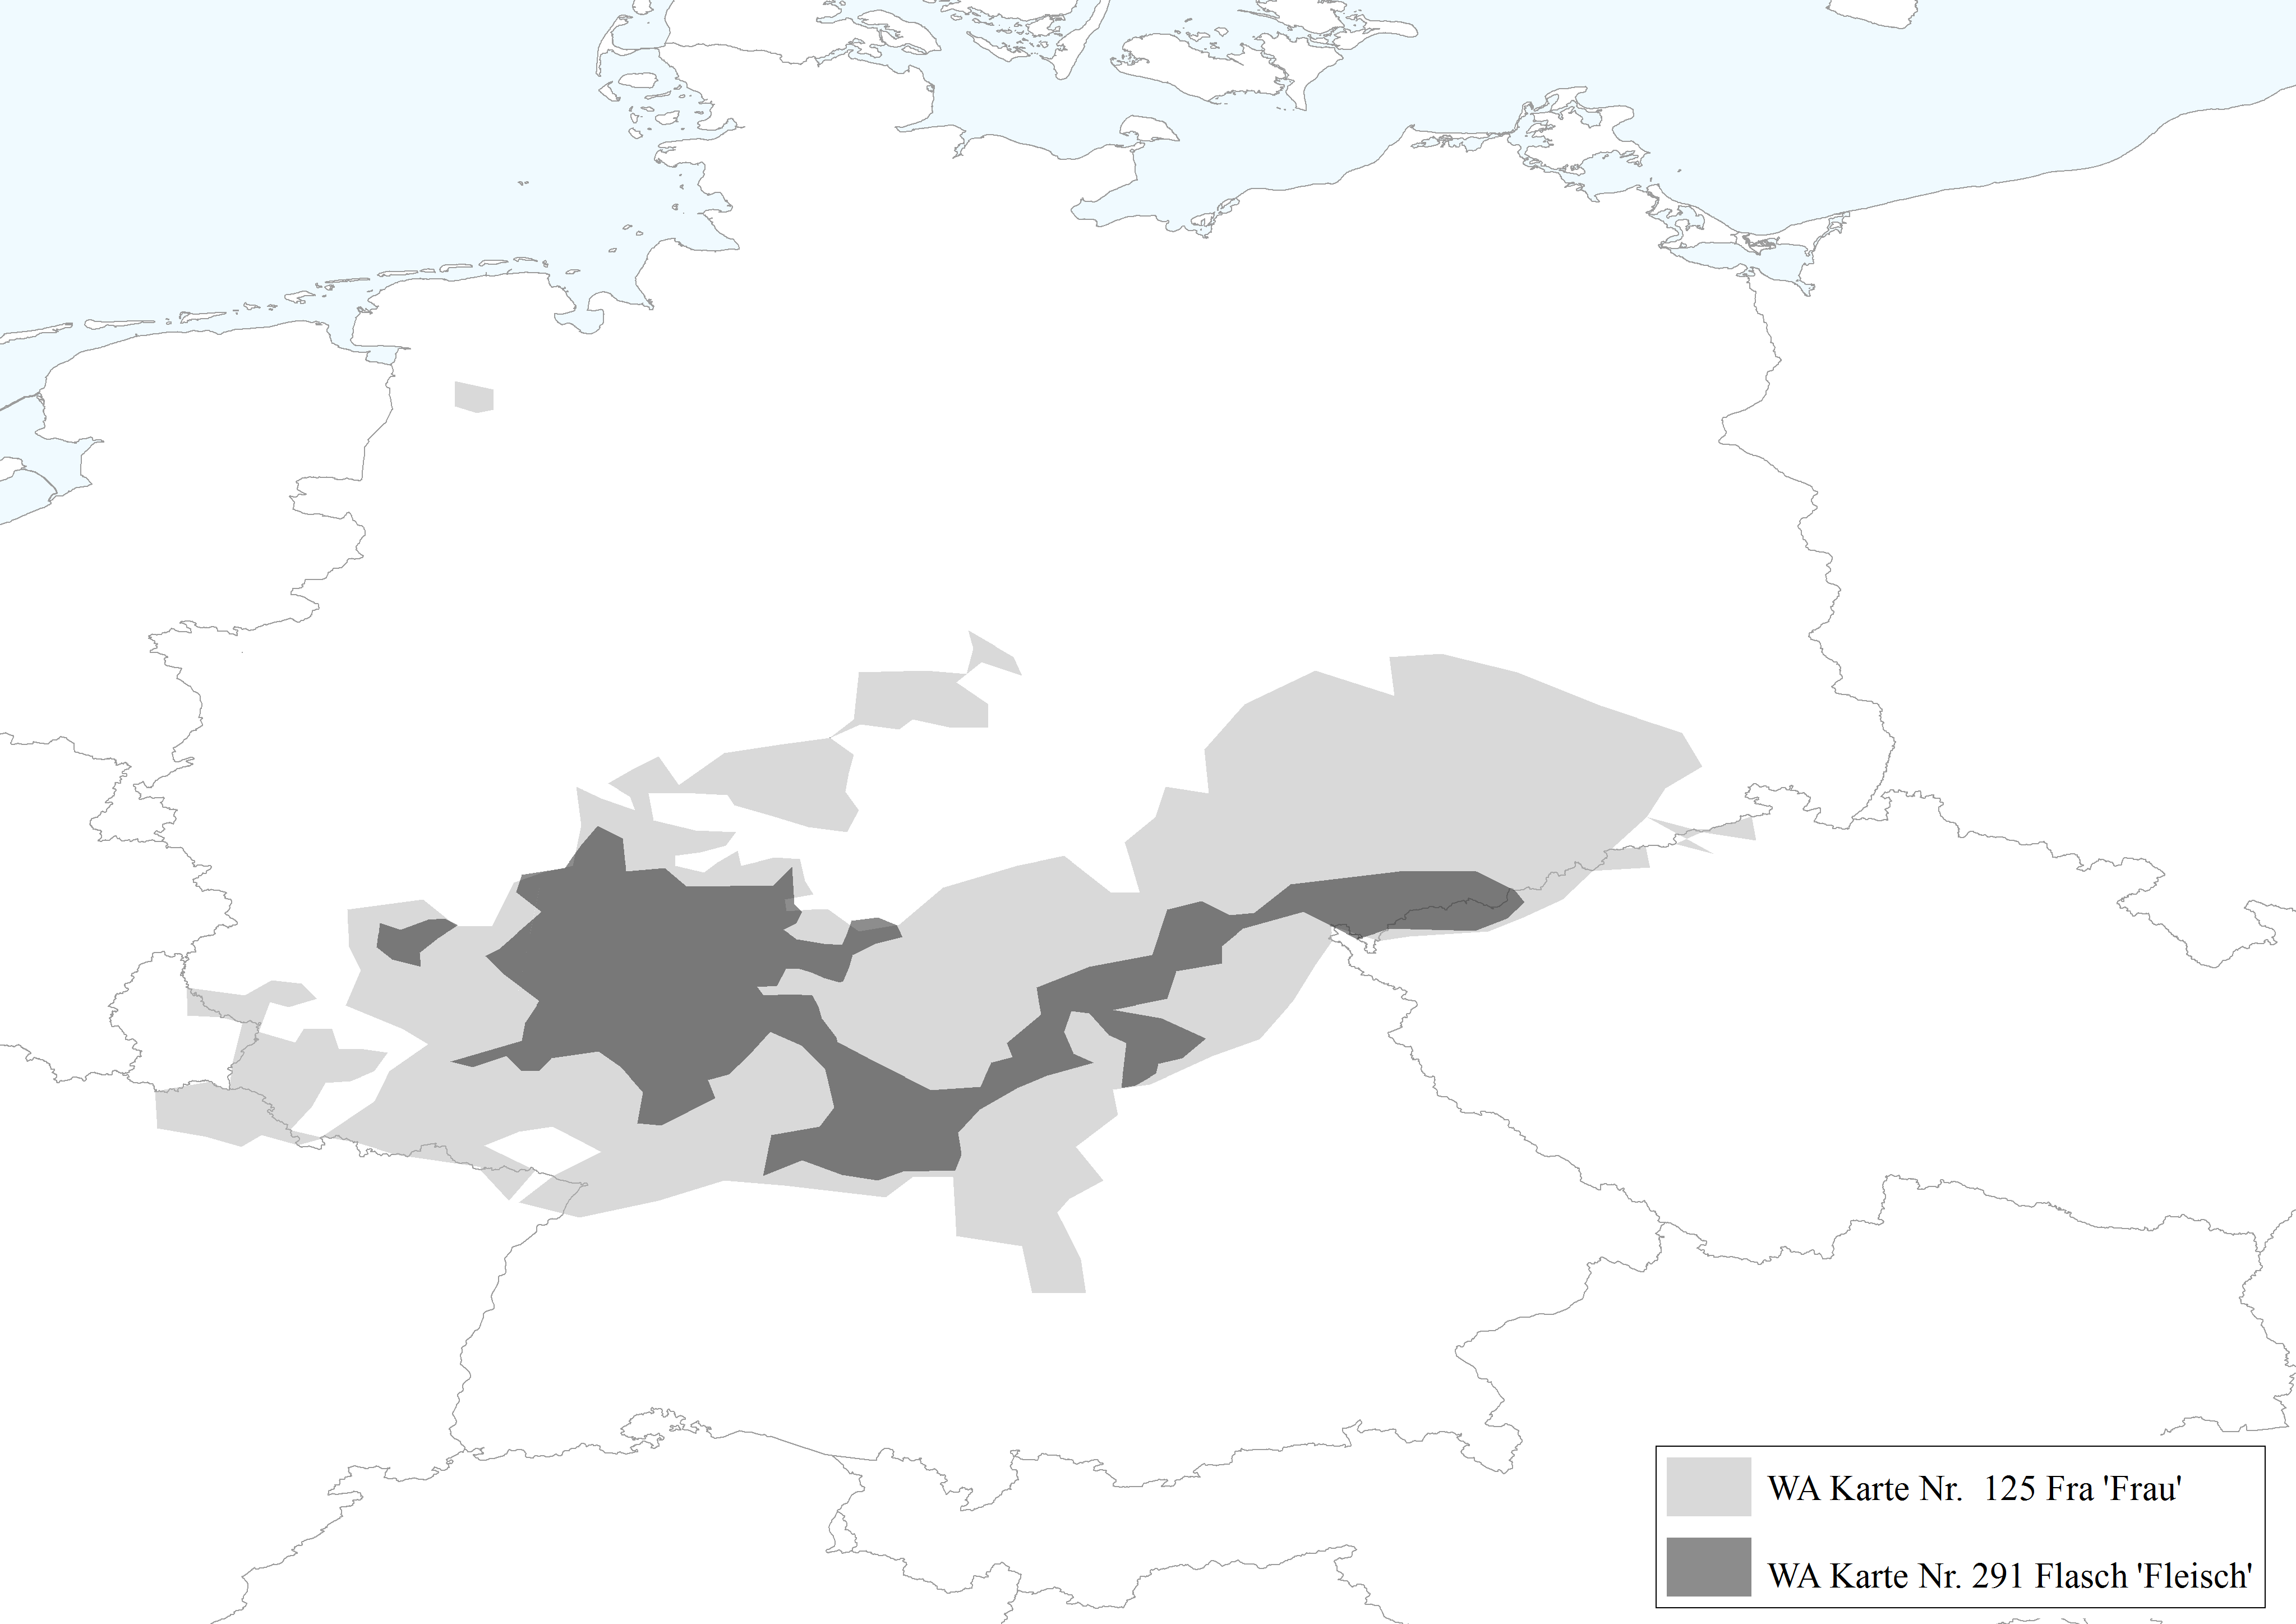
\includegraphics[width=\textwidth]{figures/dteiou.png}
		\caption{\label{dteiou} {\MHD} \textit{ou} u. \textit{ei} > /aː/ in den dt. Dialekten}
		\end{figure} 

 
\subsection{\hai{V24} (\hai{E\textsubscript{4}}, mhd. \textit{ei})}\label{phonV24}
%  %\noindent
Zunächst zur Situation des historischen Diphthongs \hai{V24} (E\textsubscript{4}) < {\urj} *\textit{ej} im \hai{{\LiJi}}. Eine Manipulation dieses Vokals findet sich im \hai{chrLiJi1}-Kernkorpus in 42 Texten. Damit weisen elf Texte keinerlei Markierung in dieser Position auf, d.\,h. hier findet sich ausschließlich ein als <ei> oder z.\,T. auch als <ey>, <ai>, <ay> wiedergegebener Diphthong, der dem Standarddeutschen gleicht. Von den 42 relevanten Texten tritt \hai{V24} als <a>, in 31 Texten längenmarkiert als <aa>  auf. Vier Texte zeigen außerdem eine Diphthongierung zu <oi>, <eu>;\, auch dieses Phänomen steht zum Teil parallel zu den gegebenen Monophthongen.  

Die geographische Streuung der Belege für eine Manipulation von {\mhd} \textit{ei} zeigt, dass wir den westjiddischen Monophthong in beinahe allen Regionen finden (vgl.\, Abbildung \ref{karteV24DSA}). Eine Ausnahme bildet der äußerste Nordosten, wo keine bzw. nur eine diphthongische Manipulation vorliegt. Besonders viele Quellen mit dem westjiddischen Langvokal finden sich in Berlin, Leipzig, Bonn, Mannheim, Frankfurt und Wien.\footnote{Der Durchmesser der Diagramme in Abbildung \ref{karteV24DSA} ist abhängig von der Anzahl der an diesem Ort relevanten Quellen.} Die Überblendung der Korpusdaten mit dem Areal von /\textit{a\textlengthmark}/ für {\mhd} \textit{ei} im Lexem \sem{Fleisch} in den deutschen Dialekten zeigt, dass zumindest an den Orten Frankfurt, Mannheim, Erlangen, Nürnberg und Wien ein Einwirken der deutschen Dialekte auf das \hai{chrLiJi1} nicht auszuschließen ist. 
		
		\begin{figure}
		\centering
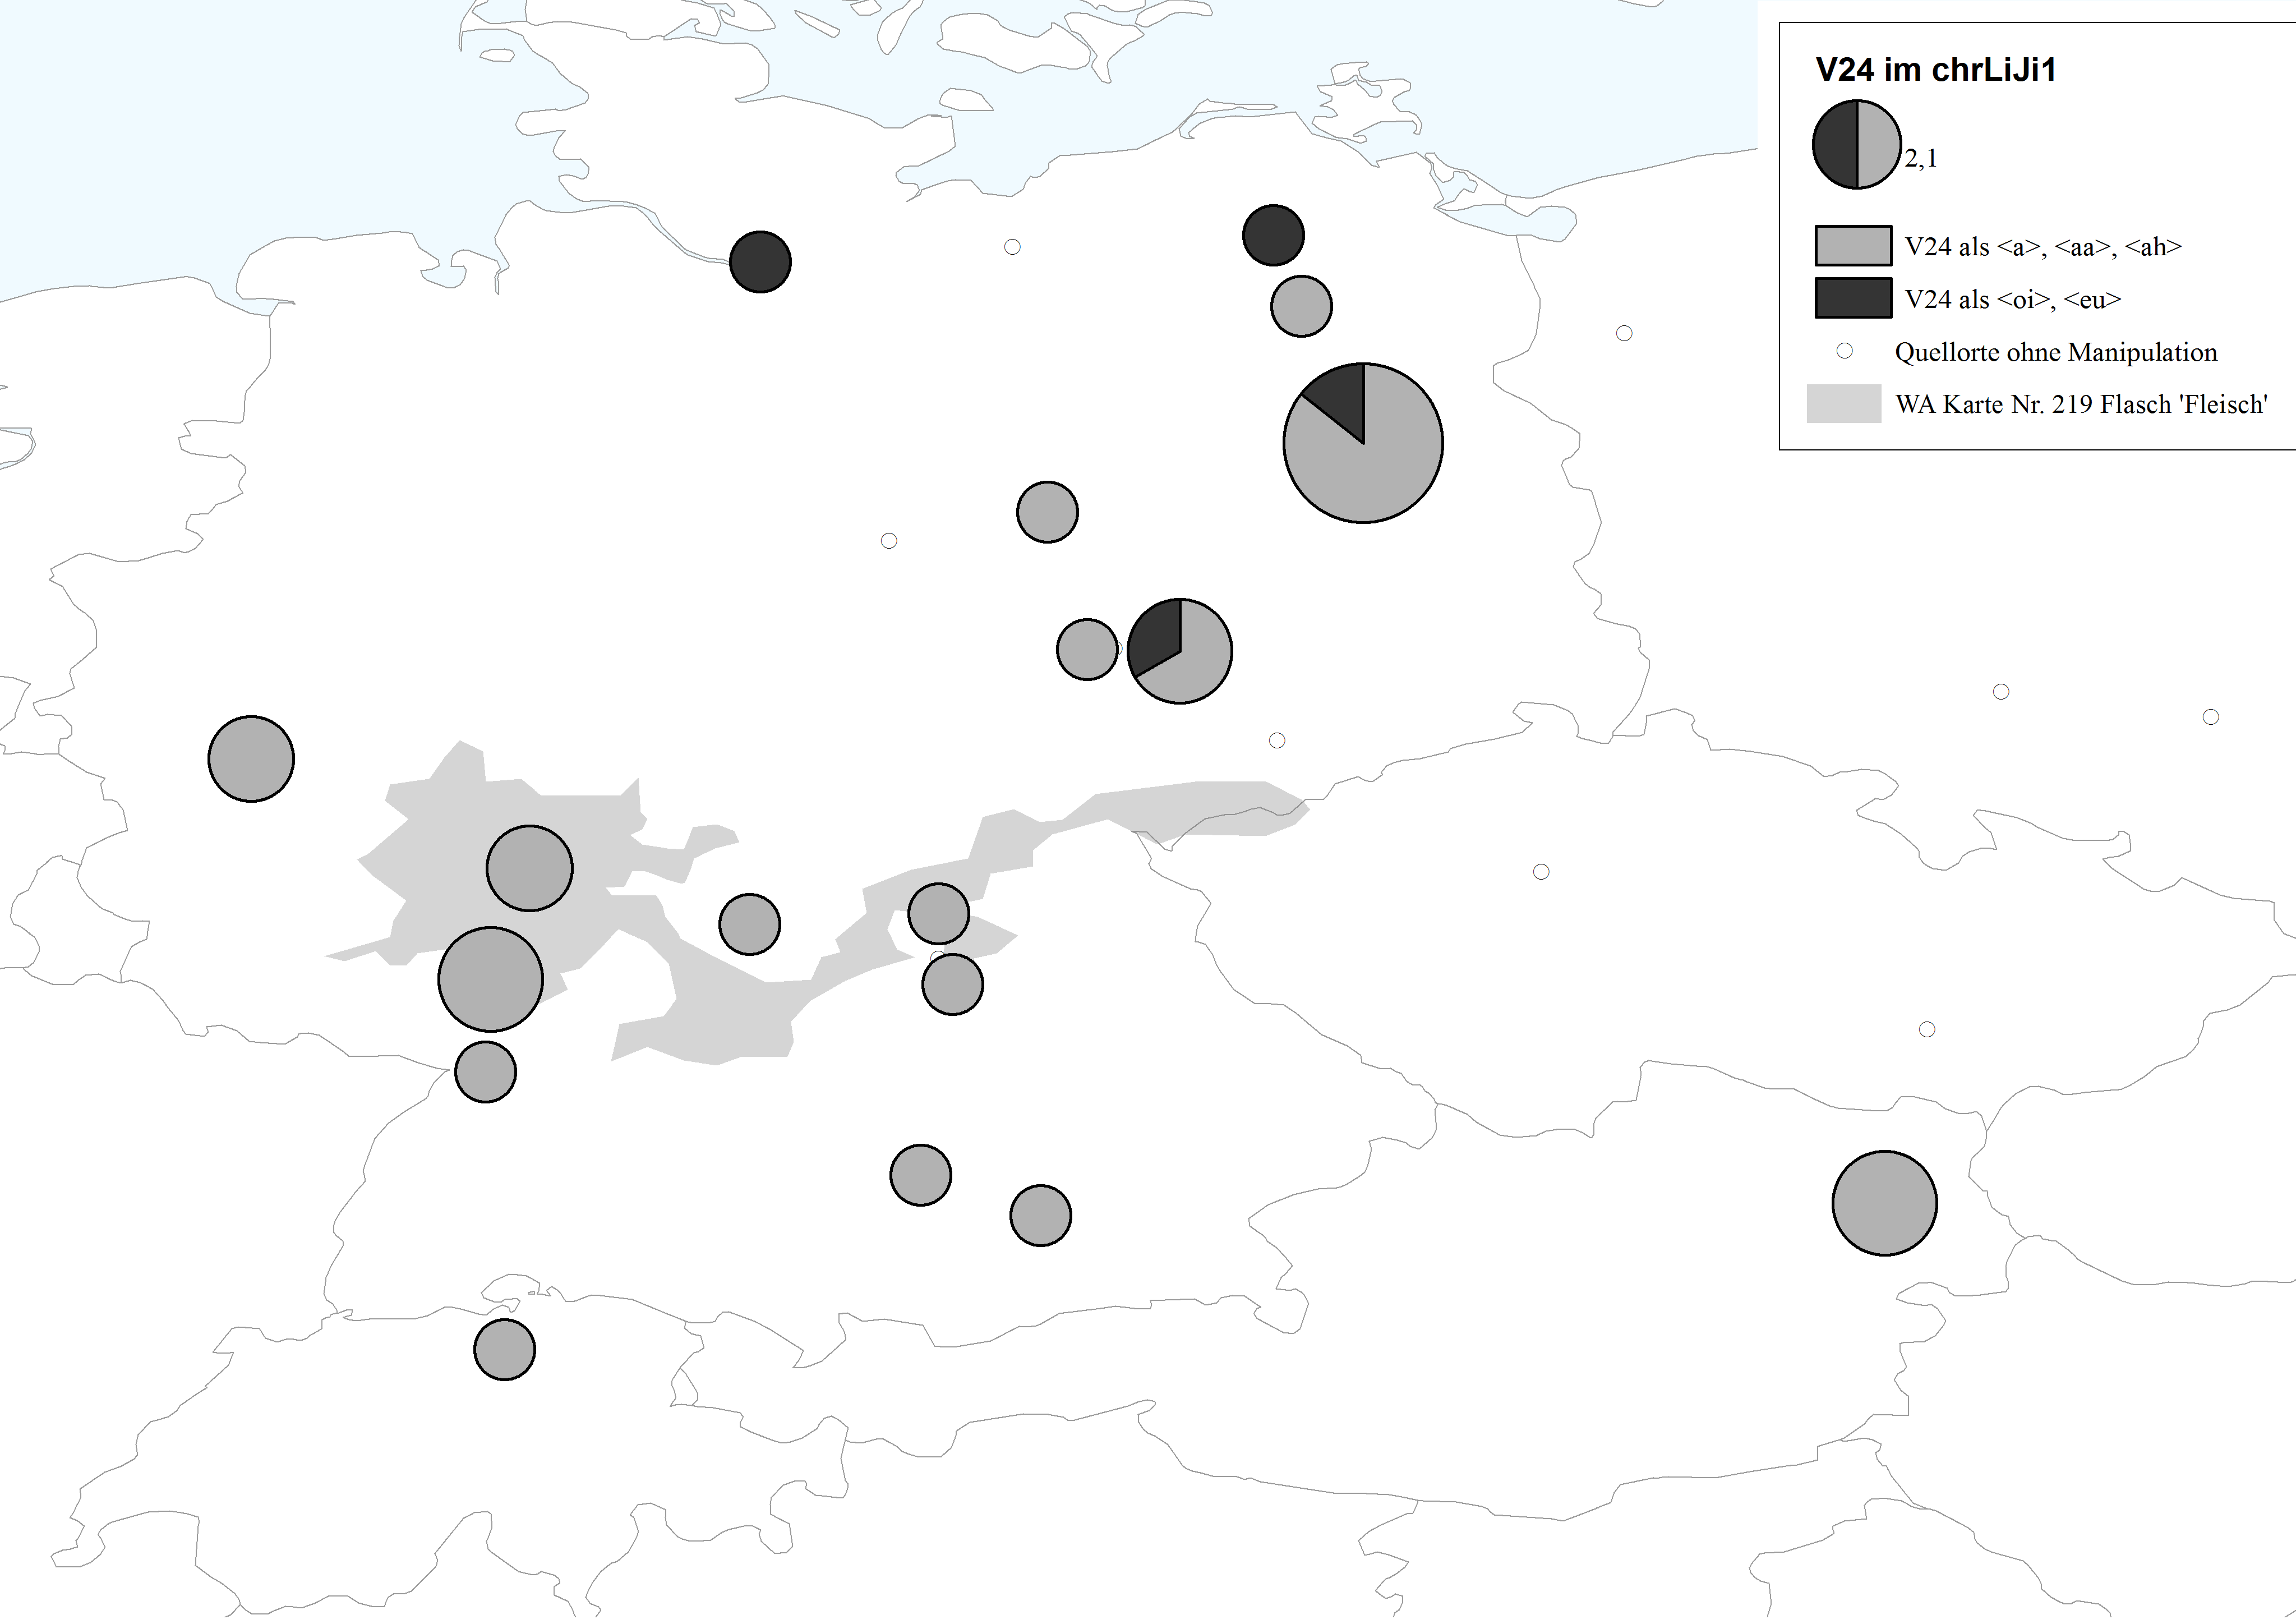
\includegraphics[width=\textwidth]{figures/V24_neuDSA.png}
		\caption{\label{karteV24DSA}  \hai{V24} im \hai{chrLiJi1} mit WA Karte Nr. 291}
		\end{figure}
 


Die in der \hai{WA}-Karte nicht abgedeckten Dialekte der Schweiz und Österreichs zeigen gemäß der entsprechenden Karte des \hai{KDSA} Nr. 417, dass hier der {\mhd} Diphthong unverändert blieb. Die Monophthongierung zu /a\textlengthmark/ ist darin lediglich in einem burgenländischen Ort aufgeführt.\footnote{Hinter diesem Ortspunkt könnte sich der westjiddische Wenkerbogen aus Frauenkirchen (\hai{WB} Nr. 42663) verbergen;\, der  \hai{KDSA} ist leider nicht transparent, welche Bögen in sein Sample einflossen.}
Tatsächlich ist die Monophthongierung von {\mhd} /ei/ > /a\textlengthmark/ aber in vielen modernen süd- und mittelbairischen Dialekten Österreichs belegt (vgl.\, \citealt{Wiesinger2001}). \cite[233]{Schirmunski1962} wie auch \cite{Wiesinger2001} geben an, dass die Monophthongierung zu /a\textlengthmark/ < {\mhd} \textit{ei} besonders in \qu{Wien und andere[n] österreichische[n] Stadtmundarten} stattgefunden hat, also kein basisdialektales Phänomen darstellt. Für die hier relevante Wiener Stadtmundart zeigt Wiesinger (\citeyear[92f]{Wiesinger2001}), dass bereits Ende des 19. Jahrhunderts der \qu{prestigeträchtige Wiener städtische
 Monophthong} stark auf die Dialekte der niederösterreichischen Landbevölkerung gewirkt hat. In Wien selbst ist ein Monophthong an der Position von {\mhd} \textit{ei} seit dem späten 12. Jh. belegt (vgl.\, \citealt[113]{Wiesinger2001}). Die Wiener Quellen könnten demnach bei der Manipulation auf eine entsprechende Form im örtlichen deutschen Dialekt zurückgegriffen haben.
 
 Besonders interessant ist die Verteilung der Belege für <eu>, <oi> < {\mhd} \textit{ei}. Diese lassen sich mit keinem Einfluss der deutschen Mundarten erklären.\footnote{Ein entsprechender Diphthong /\textipa{\textopeno\textsubarch{I}}/ < {\mhd} \textit{ei} ist in den deutschen Dialekten nur im \ili{bairisch}-alemannischen Übergangsgebiet zu finden (vgl.\, \hai{WA} Karte Nr. 219).} Bei diesen Belegen ist zu vermuten, dass dieser Diphthong als Kennlaut für (Ost)jid\-disch verwendet wurde, obwohl er in dieser Position keinerlei Entsprechung im Jiddischen hat.\footnote{Im \hai{{\OJ}} unterscheidet sich \hai{V24} ({\mhd} \textit{ei}) als Diphthong [ej] nur wenig vom Schriftdeutschen.} Erstaunlich ist aber dennoch die durchaus gegebene Arealbildung von Quellen mit \hai{V24} als <eu>, <oi> im Nordosten. Da es keinen Grund dafür gibt, anzunehmen, dass diese Formen in irgendeiner Weise auf tatsächliche Sprachgegebenheiten referieren, ist zu vermuten, dass es sich hierbei um Hyperkorrekturen handelt, die den ostjiddischen Diphthong von \hai{V44} ({\mhd} \textit{ou}) und \hai{V42}/\,\hai{V43} ({\mhd} \textit{ô}) auf \hai{V24} übertragen. Dies ließe zwei weitere Schlüsse zu, die das Areal im Nordosten erklären: Zum \,%rs groß
 einen mag der Einfluss des Ostjiddischen in dieser Region stärker gewesen sein als andernorts,  zum anderen könnte die Unsicherheit bzw. Fehlerhaftigkeit bei der \isi{Imitation} des Jiddischen darauf schließen, dass im Nordosten \ili{Westjiddisch} weniger vital war als im übrigen Untersuchungsgebiet. Für letztere Erklärung sprechen auch die Daten der diachronen Verteilung dieser Belege (Abbildung \ref{V24}). Das Histogramm zeigt deutlich, dass der Diphthong <oi>, <eu> (/\textipa{\textopeno\textsubarch{I}}/) erst ab der zweiten Jahrhunderthälfte des 19. Jahrhunderts auftaucht, also zu einem Zeitpunkt, an dem der \isi{Sprachtod} des Westjiddischen bereits fortgeschritten ist. Zwar finden sich noch authentische \hai{A1}-Quellen aus dem Nordosten für die erste Hälfte des 19. Jahrhunderts, wie etwa die Kindheitserfahrungen der Autobiographie A.\,H. Heymanns (1803–1880) aus Strausberg (Berlin) (vgl.\, \citealt{Schaefer2013}), doch ab der zweiten Jahrhunderthälfte liegt kein authentisches Datum des \hai{A1}-Typs aus dieser Region vor.\footnote{Aus dem Nordwesten sind immerhin die recht jungen Quellen aus Aurich überliefert (Reershemius \citeyear{Reershemius2007}, \citeyear{Reershemius2014}).}
 
 Diachron streuen die Belege für den westjiddischen Monophthong von {\mhd} \textit{ei} sehr weit (s. Histogramm in Abbildung \ref{V24}). Den westjiddischen Langvokal finden wir überwiegend zwischen 1775 und 1870. Nach dieser Periode tritt dieses Phänomen nur noch vereinzelt auf.  Auch fällt im diachronen Bild auf, dass Texte, welche auf eine Manipulation von {\mhd} \textit{ei} verzichten, leicht mit der Zeit abnehmen. Ab 1872 lässt sich  ein kurzzeitiger Einbruch von Belegen für den westjiddischen Monophthong erkennen. Insgesamt lässt sich dennoch festhalten, dass \hai{chrLiJi1} zwar nicht konsequent, aber überwiegend (in 31 von 53 Texten) den westjiddischen Langvokal einsetzt und damit die tatsächliche Sprachrealität wiedergibt.
 
 
 \begin{figure}
	\begin{tikzpicture}
		\begin{axis}[only marks, width=0.82\textwidth,height=0.2\textheight,
		legend style={at={(1,1)},xshift=+0.2cm, yshift=-0.25cm,anchor=north west,nodes=left},
			%title={Funktionstypen des sp\"aten Westjiddisch},
			xtick={1700, 1725, 1750, 1775, 1800, 1825, 1850, 1875, 1900, 1925, 1950, 1975}, ytick=\empty,
			x tick label style={/pgf/number format/1000 sep=}, 
			y tick label style={/pgf/number format/1000 sep=},
			%extra y ticks={456.1, 1022.4},
			%extra y tick labels={{456,1},{1022,4}},
			extra y tick style={grid=major,
				tick label style={, ,}},
				ymin=0.7,
				ymax=2,
			ylabel={Phänomenbelege},
			enlarge x limits=0.03]	
	
			
\addplot [mark=*, black] table [x=jahr, y=V24] {figures/V24a.txt};%1.7
%\addplot [mark=*, gray] table [x=jahr, y=V24ae] {V24ae.txt};%2
%\addplot [mark=square*, draw=black] table [x=jahr, y=V24e] {V24e.txt};%1.7
\addplot [mark=*, gray] table [x=jahr, y=V24euoi] {figures/V24oi.txt};%1.4
\addplot [mark=o, black] table [x=jahr, y=no] {figures/V24no_neu.txt};%1.1

			% Andere Formen a={mark=square*,blue},% b={mark=triangle*,red},% c={mark=o,draw=black}}
						\legend{\hai{V24} als <a> , \hai{V24} als <oi>, unmanipuliert} %macht Legende
		\end{axis}
	\end{tikzpicture}
	\caption{\hai{V24} im \hai{chrLiJi1}}
	\label{V24}	
\end{figure}


 \subsection{Der unbestimmte Artikel als Sonderfall}\label{artikelkapitel}
%  %\noindent
 Eine Ausnahme bildet das Lexem des unbestimmten Artikels \sem{ein}, weil es sich aufgrund seiner hohen \isi{Frequenz} diachron wie diatopisch anders verhält als andere Lexeme, die einen aus {\mhd} \textit{ei} hervorgegangenen Vokal beinhalten.\footnote{Dem entsprechenden Eintrag im \cite[Bd. 1, Sp. 520]{Lexer1992} zur Folge ist im Mittelhochdeutschen noch keine diatopische Variation zu erkennen.}   So wird dieses Lexem in 14 Quellen neben der Form \textit{a(n)} auch als \textit{ä(n)} oder \textit{e(n)} wiedergegeben.\footnote{Dies betrifft die Quellen \hai{AJ} (Berlin, 1825), \hai{DG} (Wien, 1858), \hai{FL} (Mannheim, 1778), \hai{GW} (n.a., ca.\, 1900), \hai{JK} (Breslau, 1810), \hai{LM} (Würzburg, 1844), \hai{MS} (Bonn, 1822), \hai{MV} (Berlin, 1862), \hai{NW} (Berlin, 1804), \hai{PF} (Augsburg, 1816), \hai{SS} (Berlin, 1907), \hai{SV} (München, 1890), \hai{TH} (Merseburg, 1820), \hai{VD} (Frankfurt, 1916).} \,%rs "." zu viel
 Doch gerade in diesem Lexem ist der Reduktionsvokal und selbst der \textit{n}-Ausfall auch in den deutschen Dialekten der Regelfall. So findet sich im Oberdeutschen verbreitet \textit{a}, im Mitteldeutschen \textit{e} und im Niederdeutschen \textit{e(n)} (vgl.\, \hai{WA} Karte Nr. 432). Hier kann demnach mehr die regionale Form auf das \hai{{\LiJi}} gewirkt haben, als eine Orientierung am \hai{{\WJ}}. Nach dem \hai{WjSA} (Karte Nr. 4) ist \textit{e} der unbestimmte \isi{Artikel} im gesamten Westjiddischen, während \textit{a} im Ostjiddischen und z.\,T. im niederländischen \hai{{\NWJ}} verbreitet ist. Dieses Bild bestätigen die \hai{{\LiJieins}}-Daten jedoch nicht. Auch der Blick auf authentische Quellen des \hai{{\WJ}}, wo der unbestimmte \isi{Artikel} sehr wohl als \textit{a} belegt ist (\ref{bspgrobein}–\ref{bsplevysein}), sprechen nicht für die Glaubwürdigkeit von Beraneks Kartenbild.

 \eenumsentence{
 \item \RL{א\makebox(-1.5,-7.5)[r]{\libertineGlyph{uni207B}}ה} \textit{ah} \sem{ein, einem, einen, eine, eines}\\
  (\qu{Die Hochzeit zu Grobsdorf} 1822:\,u.\,a.\, 1, 2, 6, 7, 10, 11) \label{bspgrobein}

 \item \RL{א\makebox(-1.5,-7.5)[r]{\libertineGlyph{uni207B}}} \textit{a} \sem{ein, einem, einen, eine, eines}\\
  (\qu{Esther. Oder die belohnte Tugend} Fürth, 1854:\,u.\,a.\, 1, 3, 4, 5, 7, 10) \label{bspestherein} 


 \item \textit{a} \sem{ein, einem, einen, eine, eines} \\
 (\qu{Grad wie bi's Lévy's} Mulhouse, 1928:\,u.\,a.\, 3, 4, 5, 6, 7, 10) \label{bsplevysein}  
 }
 
Die intertextuelle Unsicherheit und Variation lässt sich annähernd gut mit der geographischen Verteilung der Belege erklären. Die Karte in Abbildung \ref{karteV24e} zeigt, dass wir \textit{e(n)} \sem{ein} in nördlich verorteten Texten finden (mit einem Ausreißer in Wien), wo es auch die im Deutschen verbreitete Form darstellt. Im süddeutschen Gebiet, wo \textit{a(n)} \sem{ein} gebräuchlich ist, findet sich (von der bereits erwähnten Wiener Quelle abgesehen) kein Beleg für \textit{e(n)} im \hai{chrLiJi1}. Die Form des unbestimmten Artikels muss also durch die Situation im Deutschen beeinflusst worden sein. Viel interessanter als die Belege für \textit{e(n)} sind hingegen die Belege für \textit{a(n)} im Nordosten, wo diese Form in den deutschen Varietäten nicht gebräuchlich ist. Entweder sollten damit die oberdeutschen Eigenschaften des Jiddischen herausgestellt werden oder aber dies verweist tatsächlich auf eine weitere Verbreitung dieser Form als von Beraneck angenommen (vgl.\, \hai{WjSA} Karte Nr. 4).\footnote{vgl.\, insbes. (\ref{bspgrobein}), wo sich \textit{a} \sem{ein} findet, obwohl dies im örtlichen zentralhessischen Dialekt nicht gegeben ist.}\\
 

	\begin{figure}
		\centering
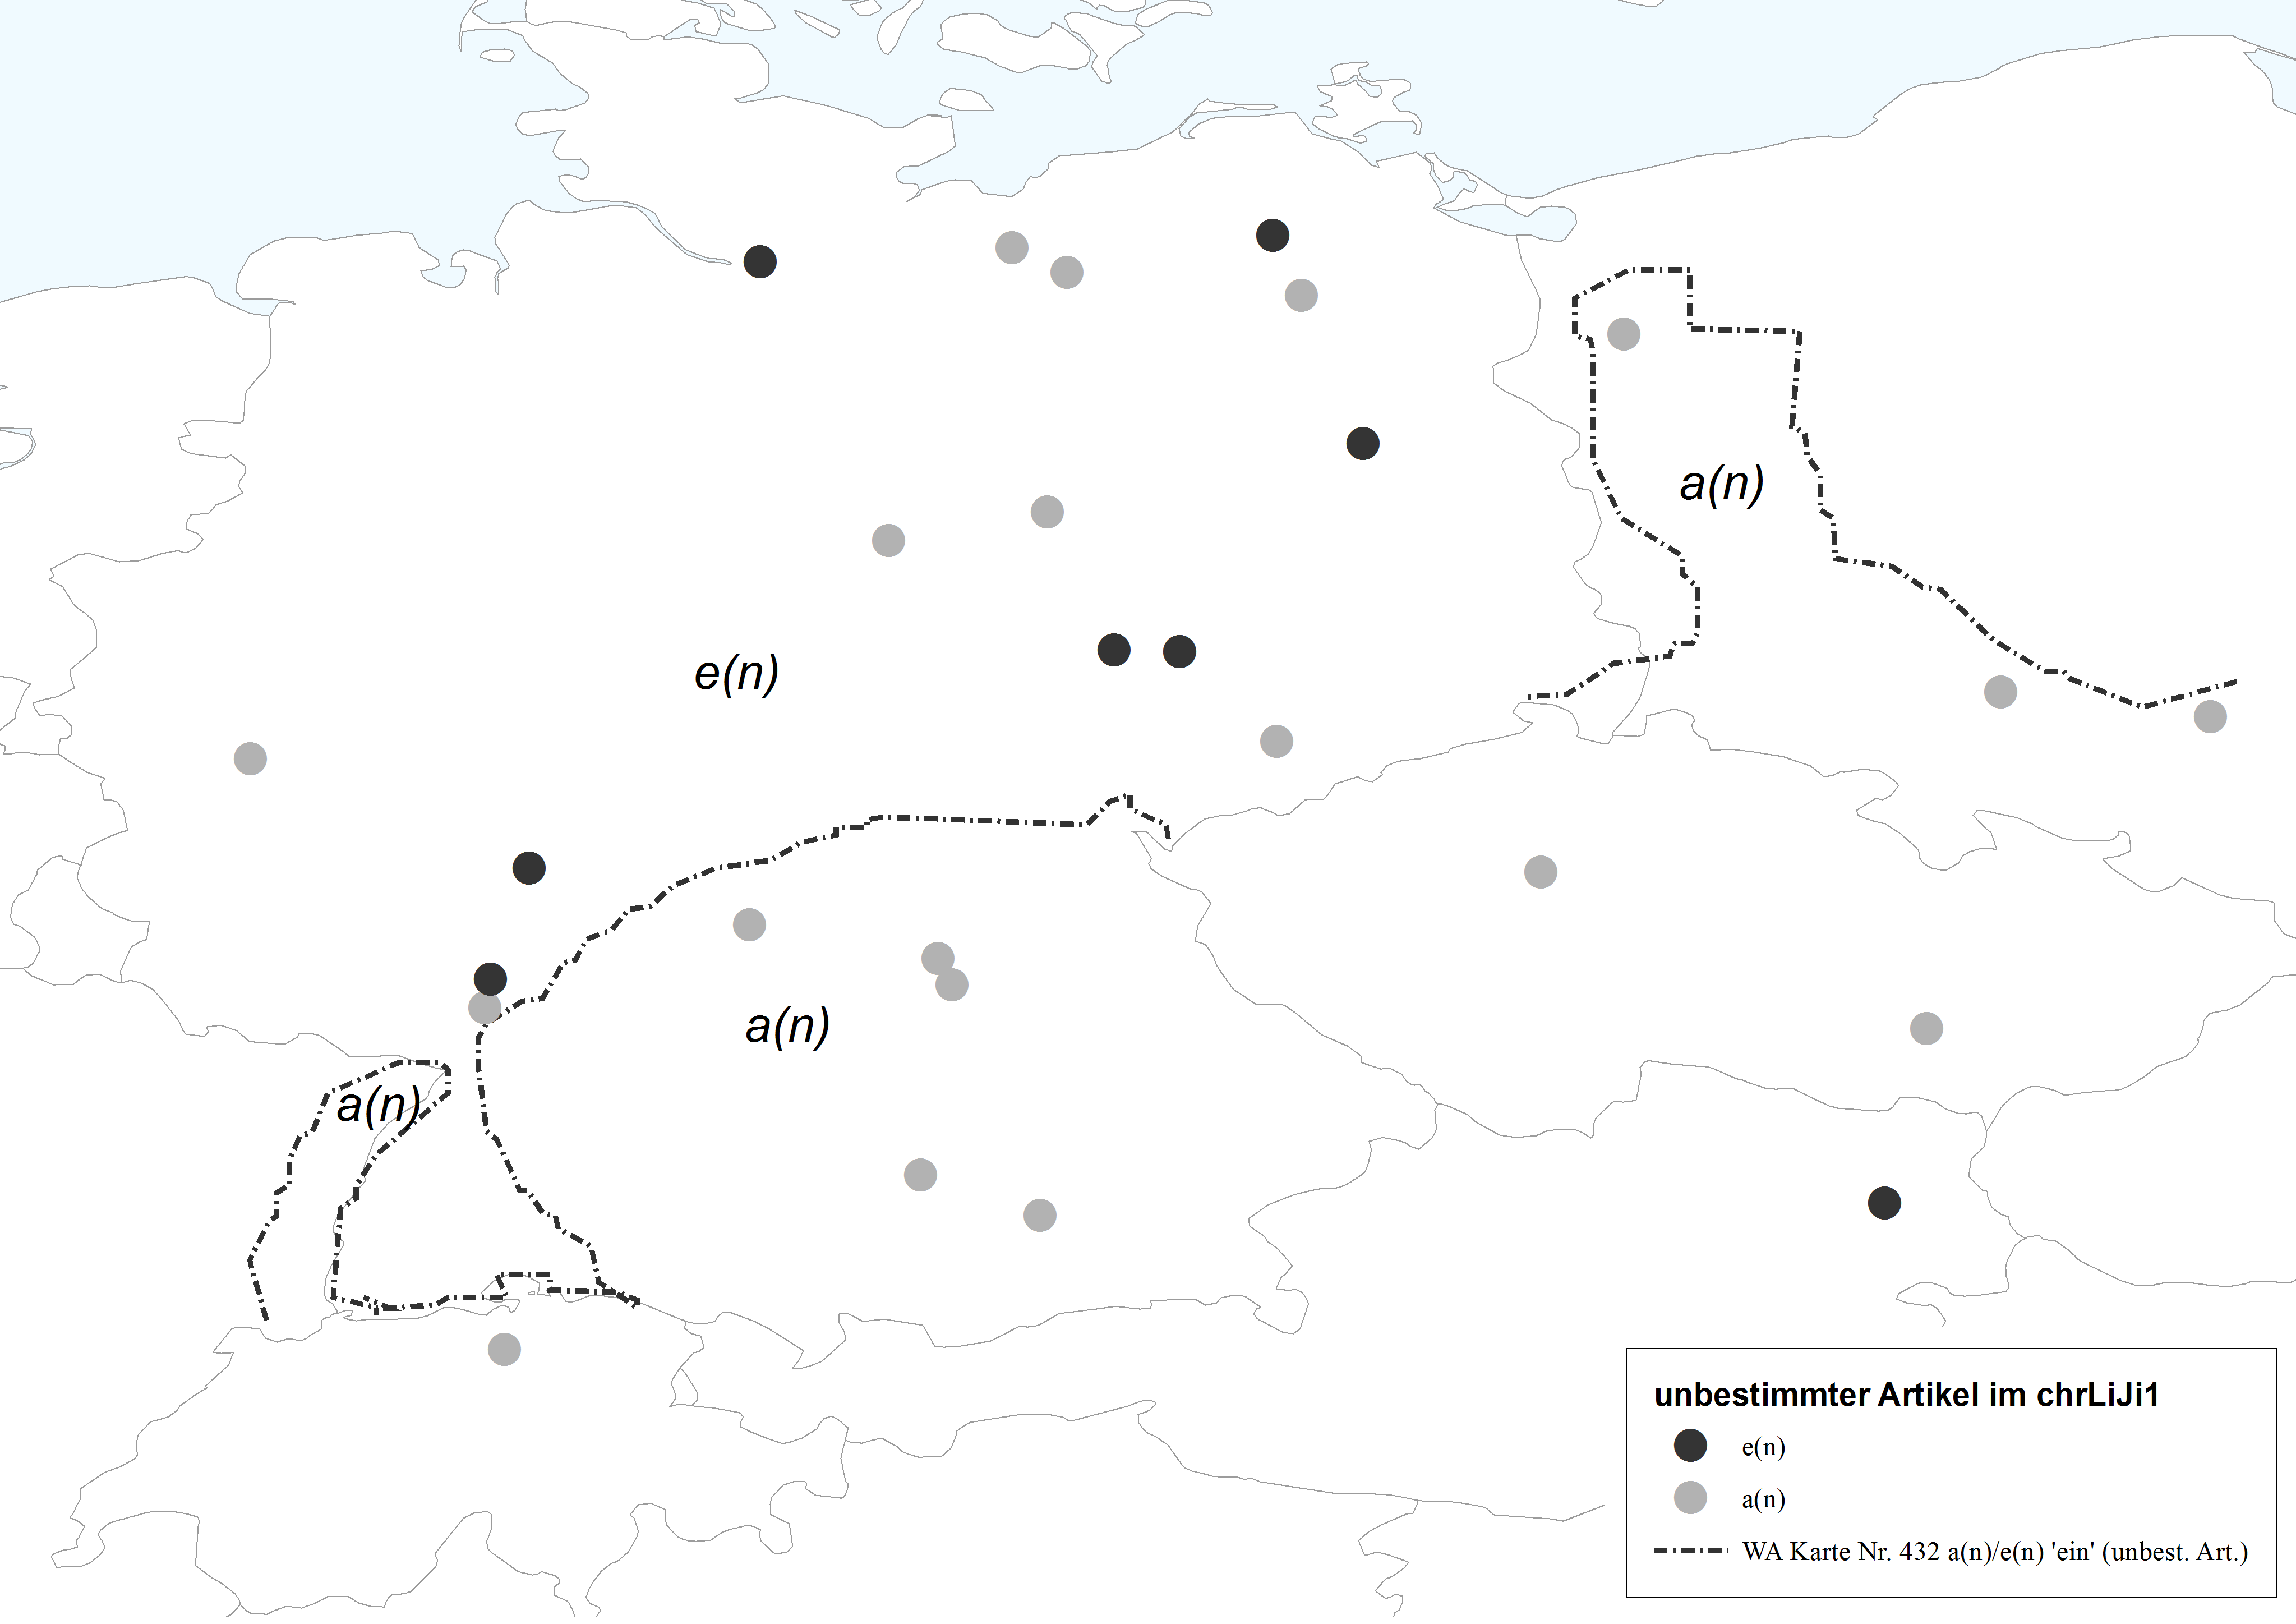
\includegraphics[width=\textwidth]{figures/V24_ein_NEU.png}
		\caption{\label{karteV24e} Der unbestimmte \isi{Artikel} im \hai{chrLiJi1} mit WA Karte Nr. 432}
		\end{figure}
 
 
 
 % \subsection{\hai{V24} im \hai{jüdLiJi1}}\label{liji2v24}
 %  %\noindent
In den Quellen des \hai{jüdLiJi1} findet sich die westjiddische Monophthongierung von \hai{V24} in neun von zehn Texten (s. Tabelle \ref{tblV24uedliji}). Auch hier gibt es eine gewisse Variation beim Vokal des unbestimmten Artikels: Nur zwei Texte (\hai{PBreslau} u. \hai{PDebrecen}) zeigen ausschließlich \textit{a(n)}, alle übrigen Quellen verwenden parallel \textit{e(n)} mit \textit{ä(n)}. 


 \begin{table}
\centering
		\begin{tabular}{lcc}
		\lsptoprule
	\textbf{Quelle} & \textbf{\hai{V24}  > /a\textlengthmark/ }& \textbf{unbest.} \textbf{{\Art}} \textbf{\textit{e(n)}}, \textbf{\textit{ä(n)}} \\ \midrule % horizontale Trennlinie
\hai{GuS1}	&  \checkmark&	\checkmark	\\
\hai{GuS5}	&	\checkmark &	\checkmark	\\
\hai{GuS10}	&\checkmark&	\checkmark \\
 \hai{GuS15} &	–	&\checkmark\\	
\hai{GuS23}	&\checkmark&	\checkmark	\\
\hai{PAlsleben}	&	\checkmark&		\checkmark \\
\hai{PBerlin1}	&\checkmark&	\checkmark \\
\hai{PBerlin2}	&	\checkmark	&\checkmark \\
\hai{PBreslau}	&\checkmark&–\\	
\hai{PDebrecen}&	\checkmark&–\\	\lspbottomrule
  \end{tabular} 
		 \caption{Modifikationen von \hai{V24} im \hai{JüdLiJi1}}
		 \label{tblV24uedliji}
		 \end{table}   
   

 
   
   
   \subsection{Hyperkorrekturen von nhd. /aɪ̯/ < mhd.  (\textit{î} \hai{V34}, \hai{I\textsubscript{4}})}\label{hyperV24}
   %  %\noindent
\largerpage
   Jiddisch hat die sogenannte \qu{neuhochdeutsche Diphthongierung} von {\mhd} \textit{î}, \textit{iu}, \textit{û} und Monophthongierung von {\mhd} \textit{ie}, \textit{uo}, \textit{üe} vollständig mitgemacht  \parencite[14–18]{Timm1987}. {\MHD} \textit{î} ist in weiten Teilen des Ostjiddischen und vollständig im Westjiddischen als Diphthong /aɪ̯/ belegt, nur im \hai{{\ZOJ}} und \hai{{\SOJ}} wurde der Diphthong wieder zu einem Monophthong /a\textlengthmark/, /a/ (vgl.\, \hai{LCAAJ} Karte Nr. 28;\, s.\,a. Karte in Abbildung \ref{karteV34hyper};\ref{bspV34_1}–\ref{bspV34_4}).\footnote{An dieser Stelle sei darauf hingewiesen, dass das protojiddische Vokalsystem nach \cite[161–205]{Herzog1965} die mittelhochdeutschen Langvokale \textit{î} und \textit{iu} zu ein- und demselben \qu{historischen Diphthong} {\urj} *\textit{əj:} zusammenfasst \parencite[1024]{Katz1983}. Da dieser Diphthong erst durch den \isi{Zusammenfall} von /\textit{i\textlengthmark}/ und /\textit{y\textlengthmark}/ im Zuge der \quein{neuhochdeutschen Diphthongierung} zwischen dem 12. und 16. Jahrhundert \parencite[146–149]{Koenig1978} zustande gekommen ist, kann das zusammengefallene Ergebnis kaum einen urjiddischen Zustand repräsentiert.} In den deutschen Dialekten ist {\mhd} \textit{î} lediglich in einem äußerst kleinen Gebiet des südwestlichen Moselfränkischen in wenigen Lexemen zu /a\textlengthmark/ geworden (vgl.\, \hai{WA} Karten Nr. 180, 176, 15). Dies ist damit eine sehr untypische Entwicklung im Deutschen.
   
\largerpage

    \eenumsentence{
    
    \item \hai{{\NWJ}}:  \textit{gleich} \sem{gleich}  \\
    (\qu{Das verfrühte Schulenrufen} Aurich 1902:\,4. Auftritt [\citealt[137]{Reershemius2007}]) \label{bspV34_1}
            
    \item \hai{ZWJ}: \RL{גלייך} \textit{gleykh} \sem{gleich}  \\
    (\qu{Die Hochzeit zu Grobsdorf} 1822:\,9) \label{bspV34_2}
    
    \item \hai{{\SWJ}}: \textit{gleich} \sem{gleich} \\
    (\qu{Chateïsim sinn aach Laït} Mulhouse 1929:\,5) \label{bspV34_3}
    
    \item {\oj}: \RL{גל{יי}\makebox(-1.5,-3.5)[r]{\libertineGlyph{uni207B}}ך} \textit{glaykh}    \label{bspV34_4} 

    
    \item  {\mhd}: \textit{gelîch} (Lexer Bd. 1, Sp. 812) \label{bspV34} \label{bspV34_5}
    

    
    }
   
   
   
   In elf Quellen des \hai{chrLiJi1} findet sich neben der Monophthongierung von {\mhd} \textit{ei} (\hai{V24}) in einzelnen Lexemen die Monophthongierung von nhd. /aɪ̯/ in der Position von {\mhd} \textit{î} (\hai{V34}, \hai{I\textsubscript{4}}), wie z.\,B.\, in (\ref{bsphyper1})–(\ref{bsphyper3}). Bei diesen Belegen könnte es sich um Hyperkorrekturen handeln, da den Autoren die historischen Vokale kaum bewusst sein konnten und so die Monophthongierung von \hai{V24} ({\mhd} \textit{ei})  zu /a\textlengthmark/ als Regel für nhd. /aɪ̯/ angewandt wurde. Möglich wäre aber auch, dass diese Daten Ausdruck eines Reflexes aus dem \hai{{\ZOJ}}/\hai{{\SOJ}} durch Zuwanderung von Ostjiddischsprechern ins deutsche Sprachgebiet sind. 
   
   
    \eenumsentence{
    
   \item \textit{blahb} \sem{bleibe} (\hai{DW} Wien, 1773:\,18) < {\mhd} \textit{blîben} \parencite[Bd. 1, Sp. 172]{Lexer1992} \label{bsphyper1}
   \item \textit{mahn} \sem{mein} (\hai{PA} Frankfurt, 1834:\,14, 51) < {\mhd} \textit{mîn} \parencite[Bd. 1, Sp. 2142]{Lexer1992} \label{bsphyper2}
   \item \textit{glach} \sem{gleich} (\hai{VE} Mannheim, 1784:\,62) < {\mhd} \textit{gelîch} \parencite[Bd. 1, Sp. 812]{Lexer1992}\label{bsphyper3}
    
    }
    
 
 Gegen einen ostjiddischen Einfluss spricht die historische Streuung der Daten (s. Abbildung \ref{V34i}). <a>, <aa> findet sich besonders in den einhundert Jahren zwischen 1775 und 1875, tritt später aber nur mehr in einer Quelle (\hai{AK} Zürich, 1948) auf. Die Belege dieser Quelle, die generell relativ viele ostjiddische Merkmale aufweist, können zwar auf die zentralostjiddischen Formen zurückgeführt werden. Dadurch, dass aber kein Anstieg der ostjiddischen Formen im Verlauf des 19. Jahrhunderts zu verzeichnen ist, ist die Annahme nicht bestätigt, diese Belege seien durch ostjiddische Einwanderung und den \isi{Sprachtod} des Westjiddischen begünstigt.

\begin{figure}
\fittable{
	\begin{tikzpicture}
		\begin{axis}[only marks, width=0.82\textwidth,height=0.2\textheight,
		legend style={at={(1,1)},xshift=+0.2cm, yshift=-0.5cm,anchor=north west,nodes=left},
			%title={Funktionstypen des sp\"aten Westjiddisch},
			xtick={1700, 1725, 1750, 1775, 1800, 1825, 1850, 1875, 1900, 1925, 1950, 1975}, ytick=\empty,
			x tick label style={/pgf/number format/1000 sep=}, 
			y tick label style={/pgf/number format/1000 sep=},
			%extra y ticks={456.1, 1022.4},
			%extra y tick labels={{456,1},{1022,4}},
			extra y tick style={grid=major,
				tick label style={, ,}},
				ymin=0.7,
				ymax=2.7,
			ylabel={Phänomenbelege},
			enlarge x limits=0.03]	
	
			

\addplot [mark=*, black] table [x=jahr, y=hyperV24] {figures/hyperv24dia.txt};%2
\addplot [mark=o, black] table [x=jahr, y=no] {figures/hyperv24dia_no.txt};%1

			% Andere Formen a={mark=square*,blue},% b={mark=triangle*,red},% c={mark=o,draw=black}}
						\legend{\hai{V34} ({\mhd} \textit{î}) als <a>, unmanipuliert} %macht Legende
		\end{axis}
	\end{tikzpicture}
}
	\caption{\hai{V34} ({\mhd} \textit{î}) im \hai{chrLiJi1}}
	\label{V34i}	
\end{figure}

Die areale Verbreitung in Abbildung \ref{karteV34hyper} spricht nicht eindeutig für einen Einfluss des Zentral- bzw. Südostjiddischen auf die Verwendung des Monophthongs an der Position von {\mhd} \textit{î}. Eine gewisse Affinität östlich verorteter Quellen (Wien, München, Leipzig, Berlin) zur ostjiddischen Form ist jedoch zu erkennen. Da es sich bei allen Quellorten, die diese Formen zeigen, um Großstädte handelt, und damit um Orte, an denen die ostjiddische Zuwanderung im 19. Jahrhundert besonders stark war (vgl.\, \citealt{Lestschinsky1960}), spricht jedoch wiederum einiges dafür, dass hier tatsächlich das Ostjiddische der Migranten seine Spuren im \hai{{\LiJieins}} hinterlassen hat. 
    


 	\begin{figure}
		\centering
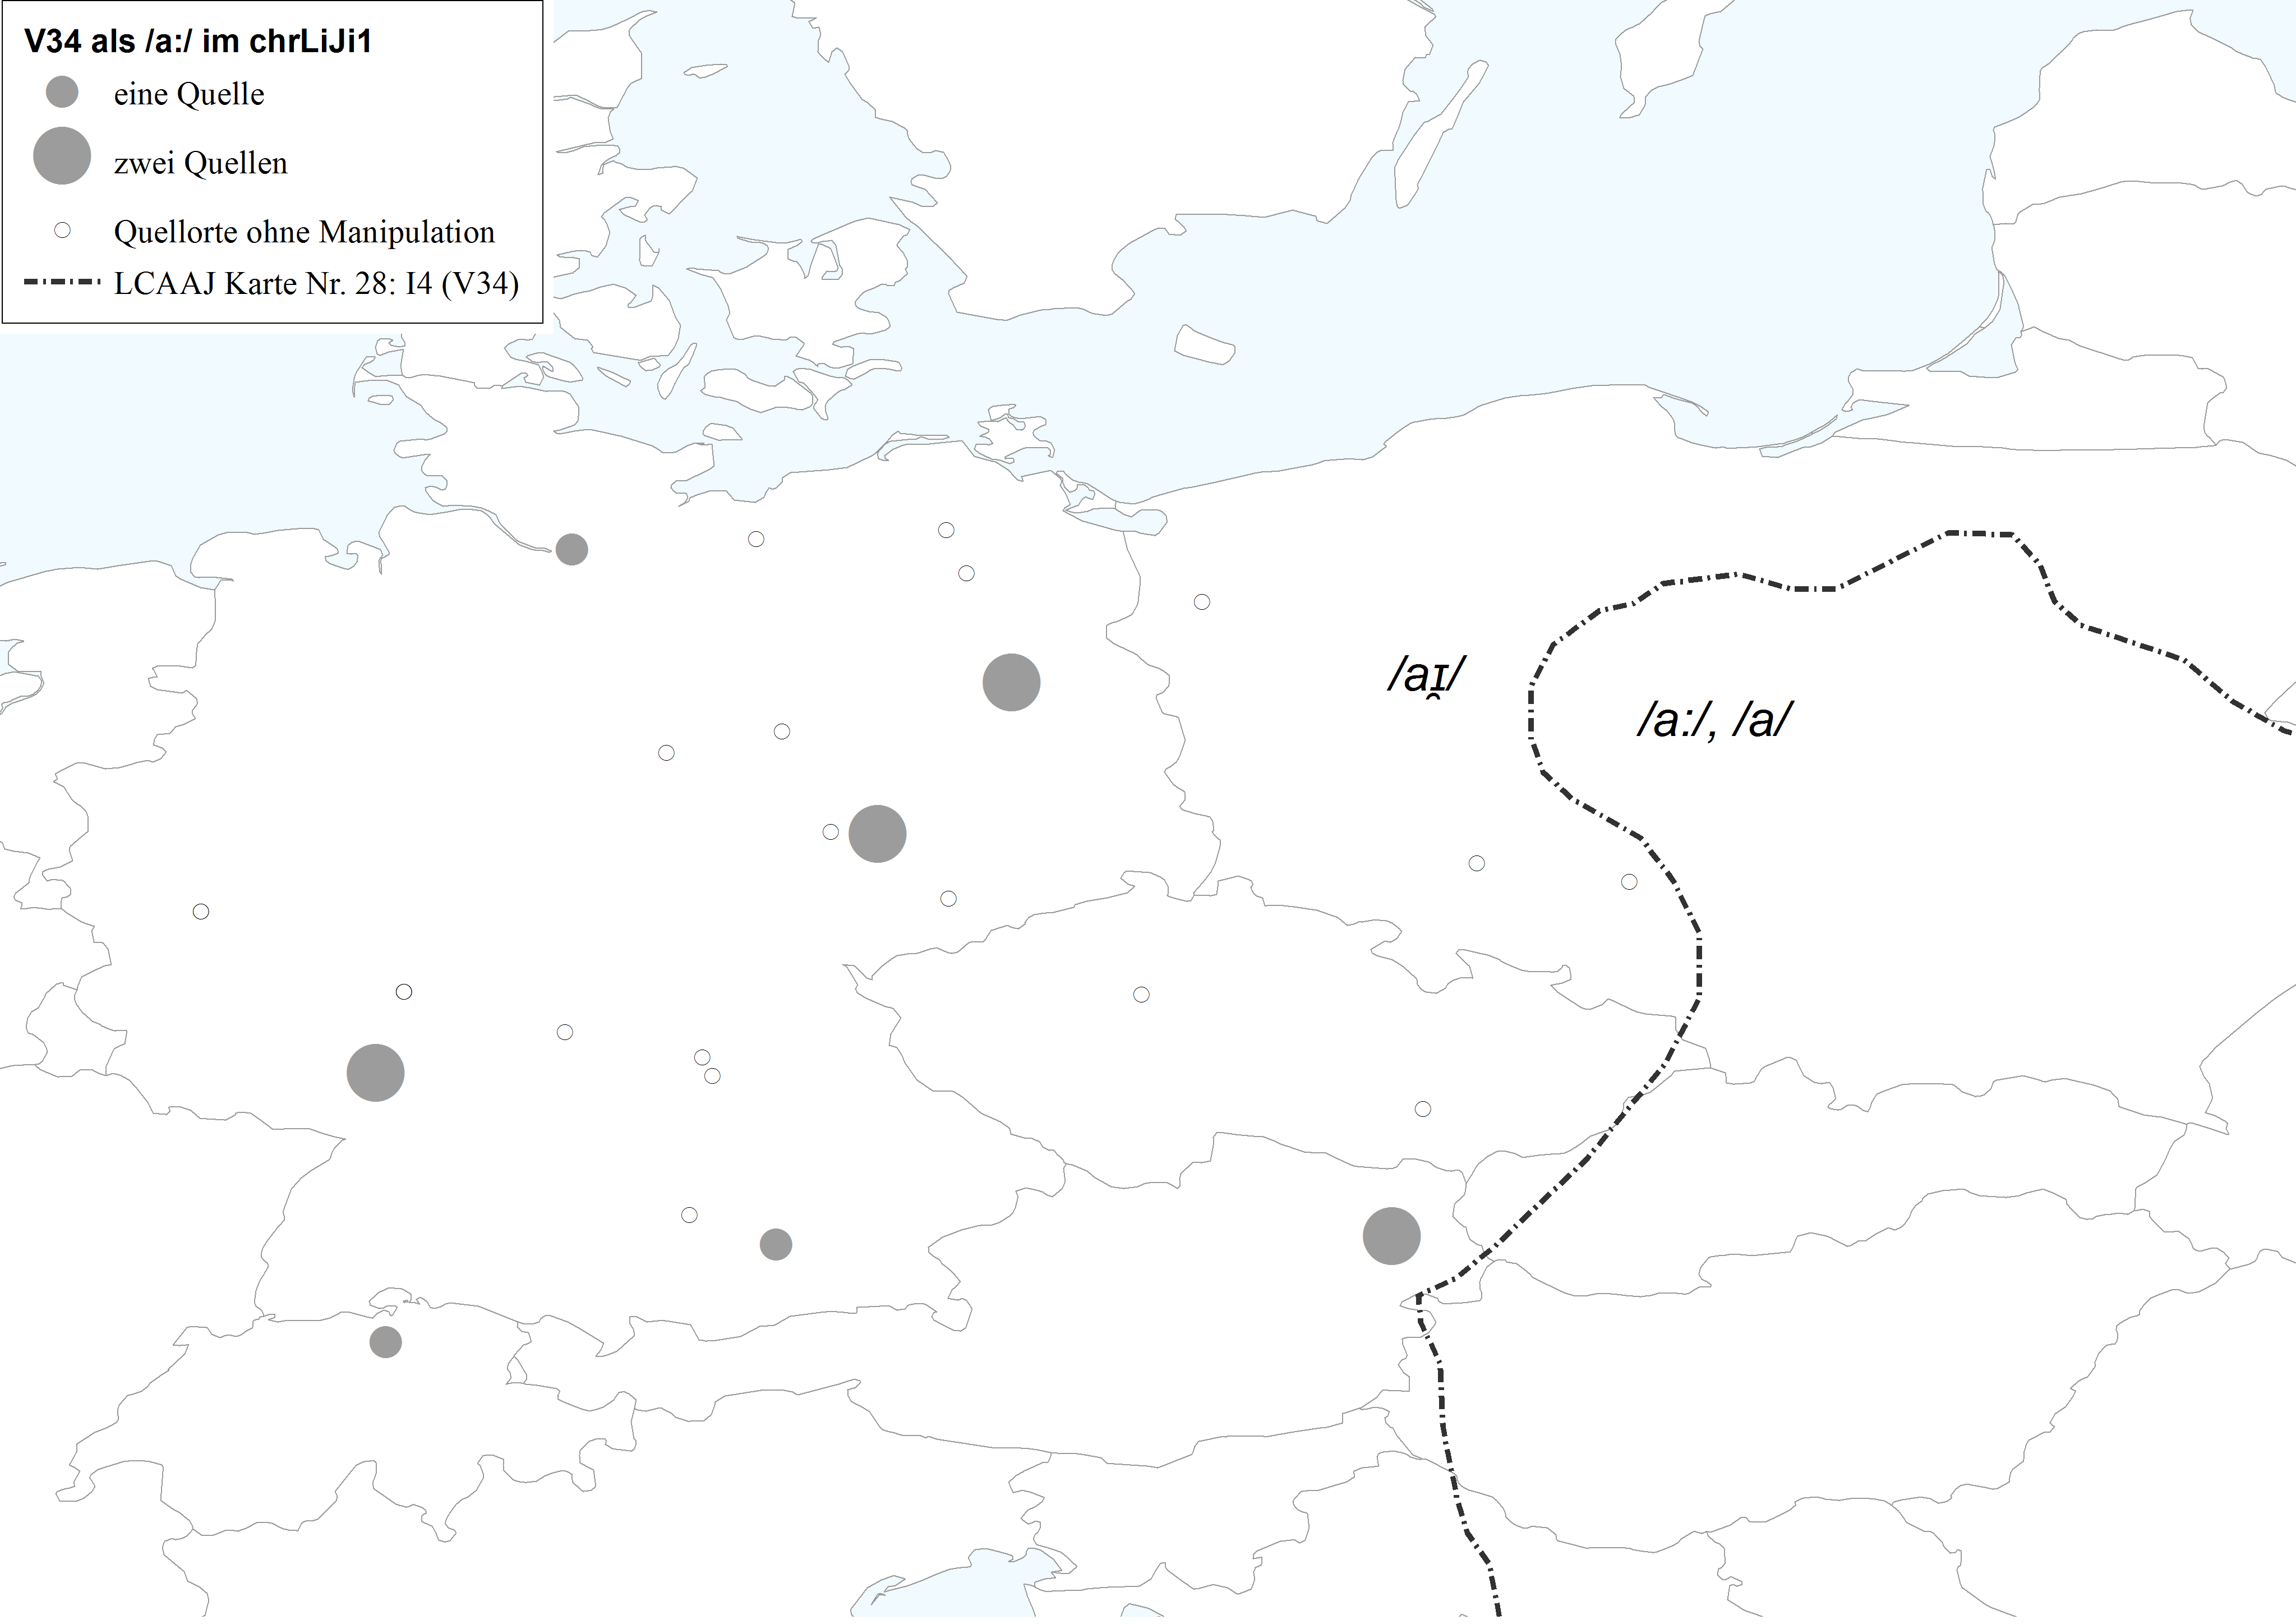
\includegraphics[width=\textwidth]{figures/hyperV34_lcaaj.png}
		\caption{\label{karteV34hyper}  \hai{V34} als /a\textlengthmark/ im \hai{chrLiJi1} mit \hai{LCAAJ} Karte Nr. 28}
		\end{figure}

 
Für einen Einfluss der ostjiddischen Dialekte sprechen besonders die Daten des \hai{jüdLiJi1}, in denen ein paar wenige solcher Formen in vier Quellen auftreten (\ref{bspV34juedliji1})–(\ref{bspV34juedliji4}).  Darunter finden sich zwei Quellen, die aus der näheren Kontaktzone zum Zentral- bzw. Südostjiddischen stammen. Der einfache Lösungsansatz bei den Belegen für {\mhd} \textit{î} als <a>, <aa> von einer Hyperkorrektur auszugehen, ist also nicht ohne weiteres zu bestätigen. Ein sich auf das Westjiddische auswirkender Einfluss des ostjiddischen Monophthongs ist jedoch in den authentischen Quellen des Westjiddischen nicht zu erkennen, s. Bsp. \,%rs Spatium fehlt
\ref{bspV34juedliji5}. Möglicherweise müssen wir bei unseren Belegen für /a\textlengthmark/ < {\mhd} \textit{î} eine Kombination aus ostjiddischem Dialekteinfluss und Hyperkorrektur annehmen. 


    \eenumsentence{
    \item \textit{saane} \sem{seine} (\hai{PAlsleben}:\,Titel, 4) \label{bspV34juedliji1}
    \item \textit{maan} \sem{meine} (\hai{PBreslau}:\,344) \label{bspV34juedliji2}
    \item \textit{was} \sem{weiß} (\hai{PDebrecen}:\,14) \label{bspV34juedliji3}
    \item \textit{maane}/\textit{mahne} \sem{meine} (\hai{GuS23}:\,10, 12) \label{bspV34juedliji4}
     \item \RL{גלייך}/\RL{גל{יי}\makebox(-1.5,-3.5)[r]{\libertineGlyph{uni207B}}ך} \textit{gleykh}/\textit{glaykh} \sem{gleich} (\qu{Die Hochzeit zu Grobsdorf} 1822:\, u.\,a.\, 9, 14, 18) 
    \label{bspV34juedliji5}
    } 
    

 
    \subsection{\hai{V44} (\hai{O\textsubscript{4}}, mhd.  \textit{ou})}\label{phonV44}
 %  %\noindent
30 von 53 Texten des \hai{chrLiJi1} weisen eine Manipulation von \hai{V44} (O\textsubscript{4}) < {\urj} *\textit{\textopeno j\textlengthmark} auf. 29 Texte zeigen dabei die Monophthongierung zu /a\textlengthmark/. Drei Texte zeigen, parallel zum Monophthong <a>, <aa> auch <o> in wenigen Lexemen auf.\footnote{Dies sind die Quellen \hai{DG} (Wien, 1858), \hai{JP} (Altona, 1867) u. \hai{WA} (Magdeburg, 1802) in \textit{lofen} \sem{laufen} (\hai{DG} Wien, 1858: 8), \textit{geglobt} \sem{geglaubt} (\hai{JP} Altona, 1867: 6R) u. \textit{globe} \sem{glaube} (\hai{WA} Magdeburg, 1802: 164).} Eine Quelle zeigt den Diphthong <äu>\footnote{Neben Belegen für den Monophthong /a\textlengthmark/ findet sich der Diphthong in \textit{gläuben} \sem{glauben} (\hai{AD} Leipzig, 1846: 137).} und eine weitere zeigt <oi>.\footnote{So belegt in der ostjiddischen Form \textit{oich} \sem{auch} (\hai{AK} Zürich, 1948: 219, 256).} 

Die diachrone Verteilung zeigt, dass der westjiddische Monophthong ab 1774 bis 1875 als Manipulationsstrategie weit verbreitet ist und zum Ende des 19. Jahrhunderts hin deutlich abnimmt (s. Histogramm in Abbildung \ref{V44}).



\begin{figure}
	\begin{tikzpicture}
		\begin{axis}[only marks, width=0.82\textwidth,height=0.2\textheight,
		legend style={at={(1,1)},xshift=+0.2cm, yshift=0cm,anchor=north west,nodes=left},
			%title={Funktionstypen des sp\"aten Westjiddisch},
			xtick={1700, 1725, 1750, 1775, 1800, 1825, 1850, 1875, 1900, 1925, 1950, 1975}, ytick=\empty,
			x tick label style={/pgf/number format/1000 sep=}, 
			y tick label style={/pgf/number format/1000 sep=},
			%extra y ticks={456.1, 1022.4},
			%extra y tick labels={{456,1},{1022,4}},
			extra y tick style={grid=major,
				tick label style={, ,}},
				ymin=0.7,
				ymax=2.7,
			ylabel={Phänomenbelege},
			enlarge x limits=0.03]	
	
			
\addplot [mark=*, black] table [x=jahr, y=a] {figures/V44a.txt};%2.3
\addplot [mark=*, gray] table [x=jahr, y=o] {figures/V44o.txt};%2
\addplot [mark=square*, draw=black] table [x=jahr, y=aeu] {figures/V44aeu.txt};%1.7
\addplot [mark=triangle*, draw=black] table [x=jahr, y=oi] {figures/V44oi.txt};%1.4
\addplot [mark=o, black] table [x=jahr, y=no] {figures/V44no.txt};%1.1

			% Andere Formen a={mark=square*,blue},% b={mark=triangle*,red},% c={mark=o,draw=black}}
						\legend{\hai{V44} als <a>/ , \hai{V44} als <o>, \hai{V44}  als <äu>, \hai{V44} als <oi>, unmanipuliert} %macht Legende
		\end{axis}
	\end{tikzpicture}
	\caption{\hai{V44} im \hai{chrLiJi1}}
	\label{V44}	
\end{figure}

 
 
 Im Vergleich zu den Manipulationsstrategien von \hai{V24} (s. Unterabschnitt \ref{phonV24}) treten im \hai{V44}-Kontext deutlich weniger Alternativen zu /a\textlengthmark/ auf. 
 Dies könnte damit erklärt werden, dass dieser Monophthong in der Entwicklung aus {\mhd} \textit{ou} auch in den deutschen Mundarten deutlich weiter verbreitet ist als der aus {\mhd} \textit{ei} (vgl.\, Karte \ref{dteiou}). 

 Mit Blick auf die areale Verbreitung der Manipulationen von \hai{V44} und der Situation von {\mhd} \textit{ou} in den deutschen Dialekten (s. Karte in Abbildung \ref{karteV44DSA})\footnote{Die Situation im Schweizer und österreichischen Alemannisch sowie im österreichischen Bairisch gestaltet sich nach der entsprechenden Karte des \hai{KDSA} Nr. 425 \,%rs Komma streichen
 so, dass hier überwiegend der standarddeutsche Diphthong /a\textsubarch{u}/ auftritt bzw. im Bodensee- und Höchstalemannischen der {\mhd} Diphthong unverändert blieb. Eine Monophthongierung zu  /a\textlengthmark/ ist in den Karten des \hai{KDSA} nicht verzeichnet. Nach \cite[235]{Schirmunski1962} findet sich im \qu{Bairisch-österreichischen […] langes ā vor -m, bisweilen vor Lippenlauten überhaupt, z. B.: Inn. bām \sem{Baum}, lāb \sem{Laub}, aber āu \sem{Auge}}. Besonders für den Wiener Stadtdialekt, 
   der für unser \isi{Korpus} eine Rolle spielt, gilt dies (vgl.\, \citealt[60–63]{SchusterSchikola1956};\citealt[33]{Bacciocco1890}). Damit sind die \hai{chrLiJi1}-Belege für /a\textlengthmark/ der Wiener Quellen auch auf eine regional verbreitete Form zurückzuführen.} \,%rs Komma streichen
   fällt auf, dass überwiegend im /a\textlengthmark/-Areal der deutschen Dialekte und in dessen unmittelbarer Nachbarschaft auch im \hai{chrLiJi1} der westjiddische Vokal auftritt. Ausnahmen bilden die Quellen im Brandenburgischen und in Hamburg, wo keine Nähe zu einem deutschen Dialekt gegeben ist, der einen entsprechenden Wandel zeigt.
 
 

 	
		\begin{figure}
		\centering
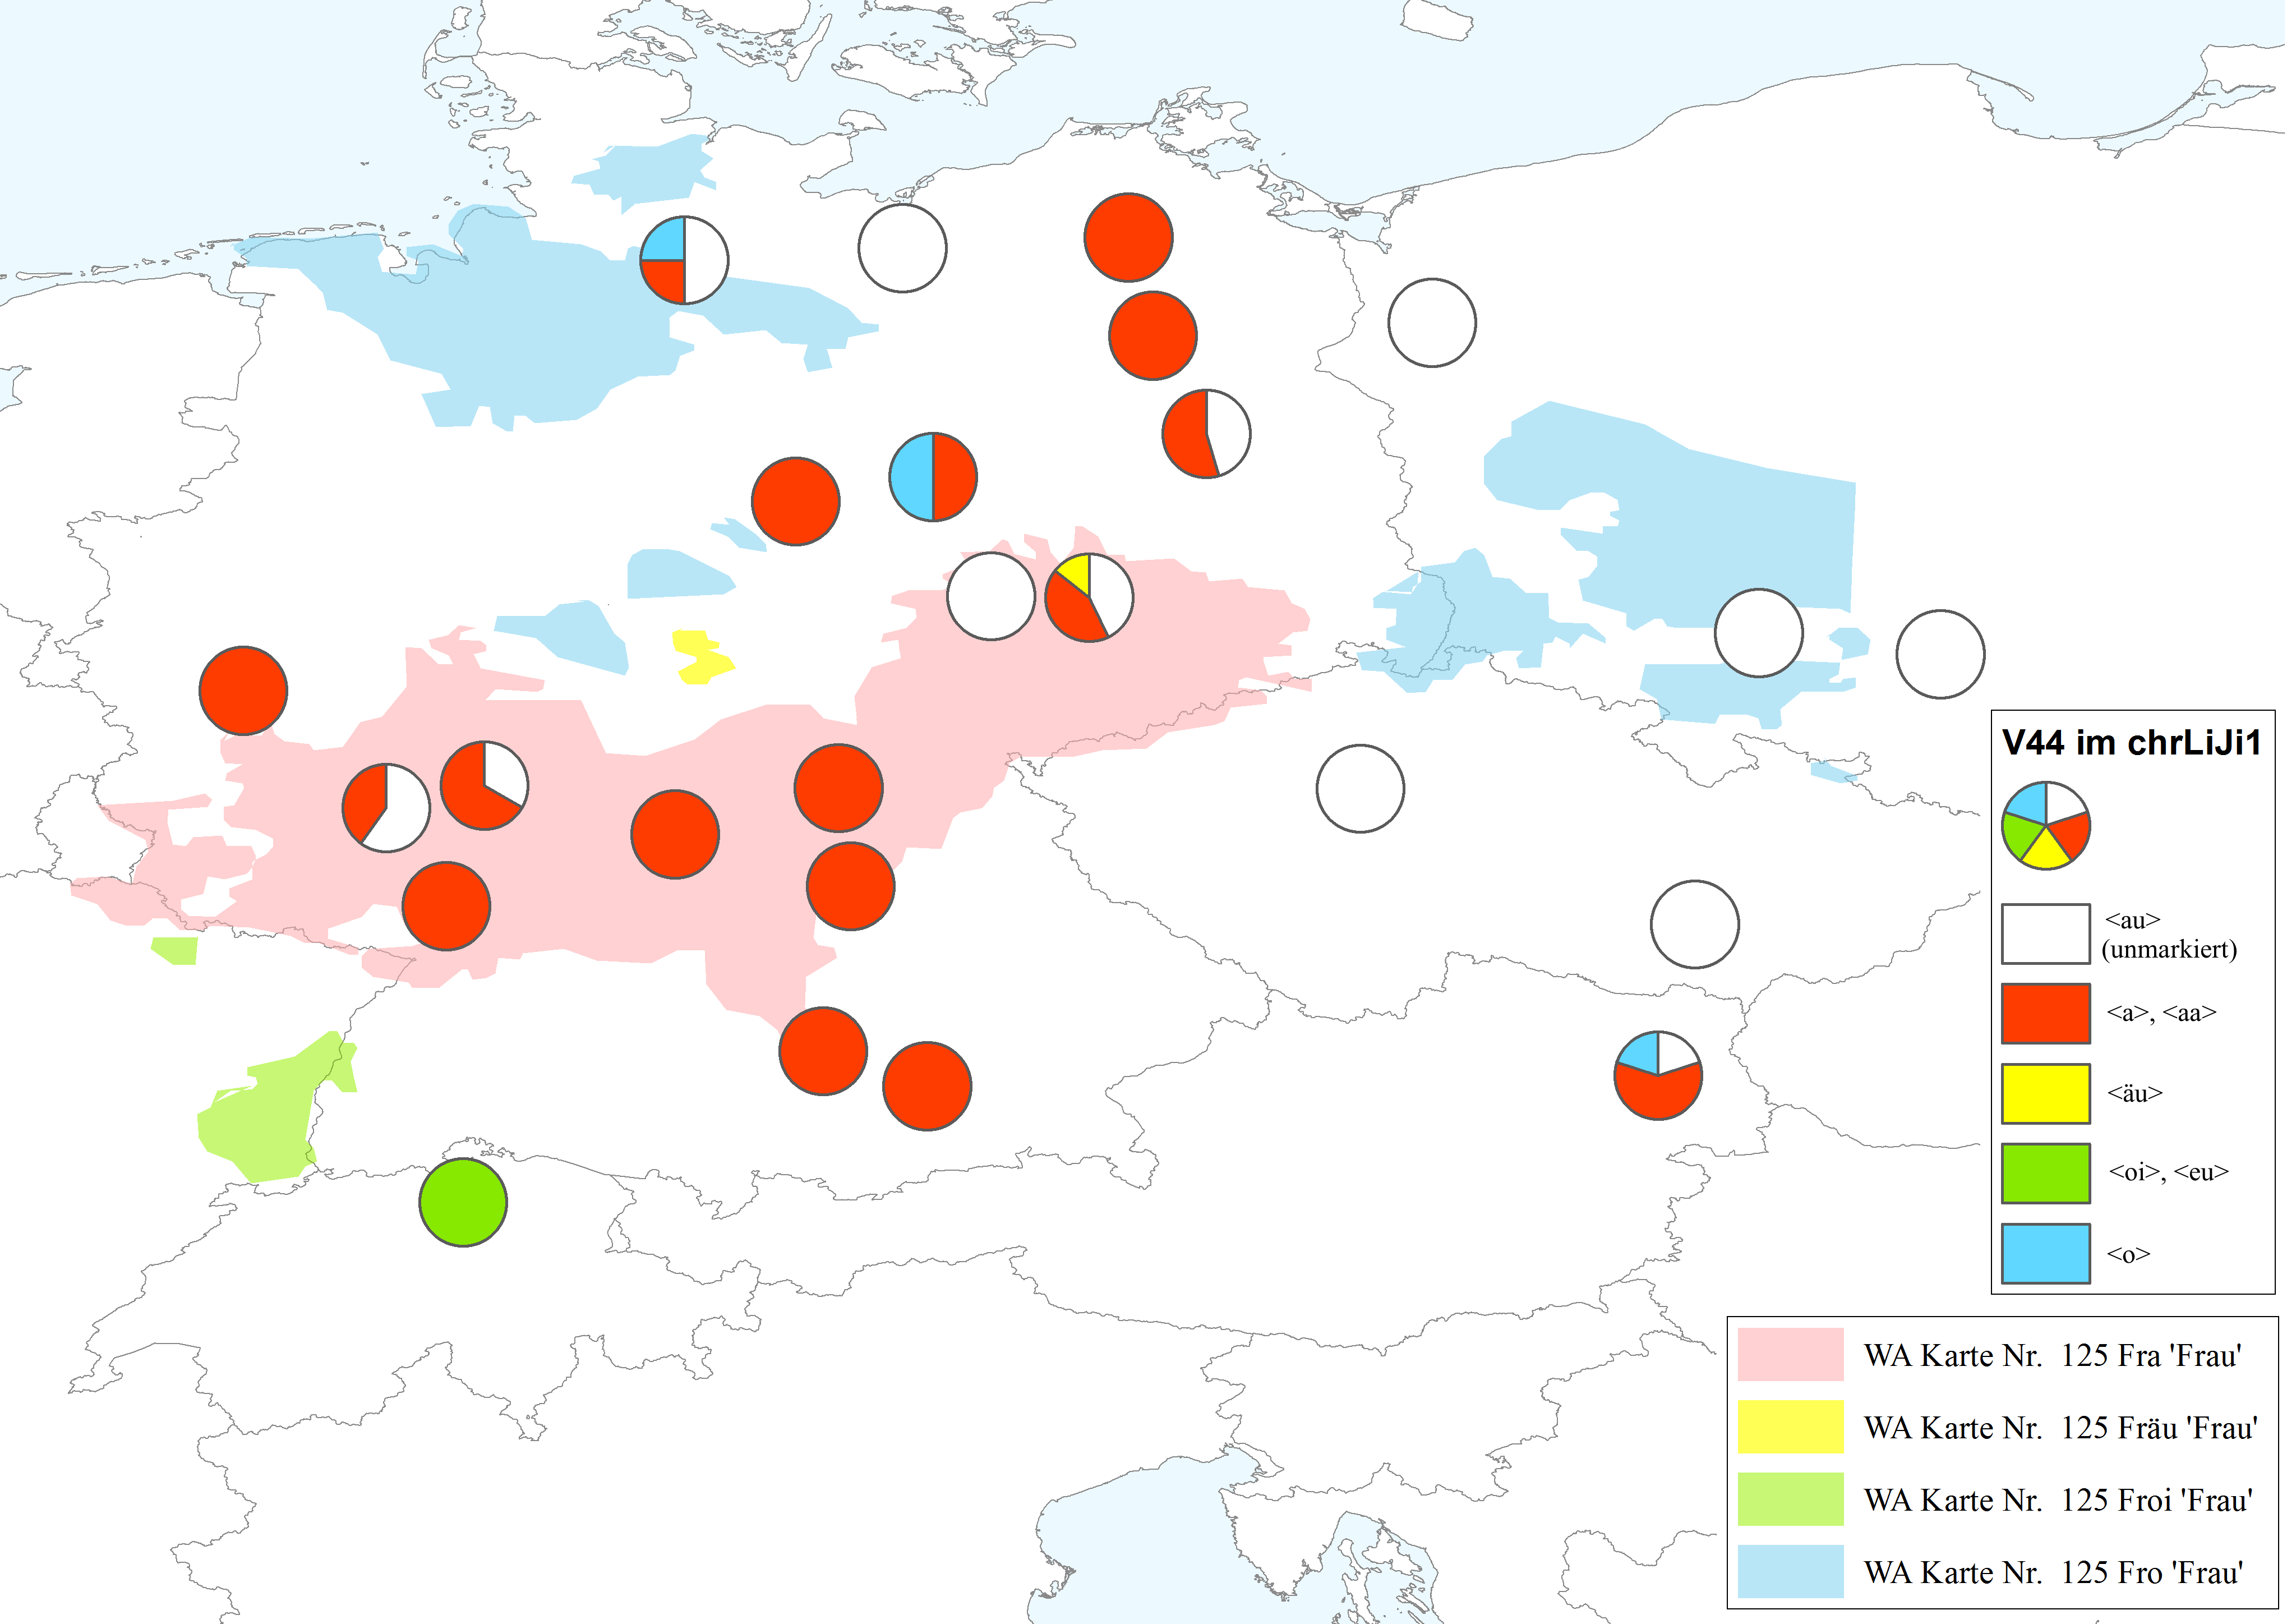
\includegraphics[width=\textwidth]{figures/V44allDSA.png}
		\caption{\label{karteV44DSA}  \hai{V44} im \hai{chrLiJi1} mit WA Karte Nr. 125}
		\end{figure}

 
 Die Situation im \hai{jüdLiJi1} zeigt ein ähnliches Bild. In allen Quellen überwiegt  die Monophthongierung von {\mhd} \textit{ou} >  /a\textlengthmark/: vier der fünf Pamphlete weisen den westjiddischen Langvokal auf. Jedoch nur zwei der fünf \hai{GuS} zeigen den Monoph\-thong. \hai{PBreslau} zeigt neben <a> eine Verdumpfung des Monophthongs zu <o> in \textit{weggelofen} \sem{weggelaufen} (\hai{PBreslau}:\, 340) und \textit{loof} \sem{lauf} (\hai{PBreslau}:\,342). In demselben Lemma findet sich diese Manipulation zu <o> auch in \hai{PBerlin1} \textit{geloffen} \sem{gelaufen} (\hai{PBerlin1}:\,3, 5, 6) und \hai{GuS5} \textit{geloffen} \sem{gelaufen} (\hai{GuS5}:\,4), hier jedoch ohne weitere Belege der westjiddischen Form. Auch \hai{PBerlin2} weist ausschließlich Belege für <o> auf, z.\,B.\,  \textit{Ogen} \sem{Augen} (\hai{PBerlin2}:\,1.Sp.), \textit{geglobt} \sem{geglaubt} (\hai{PBerlin2}:\,1.Sp.).


 \subsection{Zusammenfall von \hai{V24} und \hai{V44} > /a\textlengthmark/}\label{V24V44}
 %  %\noindent
Ein idiosynkratisches Phänomen des \hai{{\WJ}} ist nicht allein die Monophthongierung der Vokale \hai{V24} und \hai{V44}, sondern der \isi{Zusammenfall} zweier historischer Diph\-thonge zu einem Langvokal. Lediglich 16 der 53 Quellen im \hai{chrLiJi1}-\isi{Korpus} weisen diesen Wandel beider Vokale zu /a\textlengthmark/ auf.\footnote{Diese Quellen sind \hai{AO} (Wien, 1770), \hai{BW} (Leipzig, 1826), \hai{DG} (Wien, 1858), \hai{FE} (Leipzig, 1792), \hai{GP} (Nürnberg, 1831), \hai{GW} (n.a., ca.\, 1900), \hai{IA} (Erlangen, 1840), \hai{LB} (Berlin,  1785), \hai{LS} (Bonn, 1925), \hai{MS} (Bonn, 1822), \hai{NW} (Berlin, 1804), \hai{PF} (Augsburg,  1816), \hai{PM} (Magdeburg, 1792), \hai{SV} (München, 1890), \hai{VD} (Frankfurt, 1916) und \hai{WA} (Magdeburg, 1802).} Wie das Histogramm zeigt (s. Abbildung \ref{V24V44bild}), findet sich dieser \isi{Zusammenfall} sogar bis in die 1920er hinein und ist damit länger im \hai{chrLiJi1} belegt, als viele ein vitales \hai{{\WJ}} annehmen.\footnote{Die drei Quellen des 20. Jh. sind \hai{GW} (n.a., ca.\, 1900), \hai{VD} (Frankfurt, 1916) und \hai{LS} (Bonn, 1925).} Ab 1870 lässt sich allerdings ein Trend erkennen, dass dieses Phänomen nur noch sporadisch im \hai{chrLiJi1} auftritt.
 
  %%%V24 und V44Diagramm%\begin{flushleft}	
\begin{figure}
	\begin{tikzpicture}
		\begin{axis}[only marks, width=0.82\textwidth,height=0.2\textheight,
		legend style={at={(1,1)},xshift=+0.2cm, yshift=-0.2cm,anchor=north west,nodes=left},
			%title={Funktionstypen des sp\"aten Westjiddisch},
			xtick={1700, 1725, 1750, 1775, 1800, 1825, 1850, 1875, 1900, 1925, 1950, 1975}, ytick=\empty,
			x tick label style={/pgf/number format/1000 sep=}, 
			y tick label style={/pgf/number format/1000 sep=},
			%extra y ticks={456.1, 1022.4},
			%extra y tick labels={{456,1},{1022,4}},
			extra y tick style={grid=major,
				tick label style={, ,}},
				ymin=0.7,
				ymax=3.4,
			ylabel={Phänomenbelege},
			enlarge x limits=0.03]	
\addplot [mark=square*, draw=black]  table [x=jahr, y=zusammenfall] {figures/V24V44.txt};%2.3			
\addplot [mark=*, fill=white] table [x=jahr, y=V24] {figures/V24a2.txt};%2		
\addplot [mark=square*, fill=white]  table [x=jahr, y=a] {figures/V44a2.txt};%1.3


			% Andere Formen a={mark=square*,blue},% b={mark=triangle*,red},% c={mark=o,draw=black}}
						\legend{\hai{V24} u. \hai{V44} <a>, \hai{V24} als <a>, \hai{V44} als <a>}
		\end{axis}
	\end{tikzpicture}
	\caption{\hai{V24} und \hai{V44} im \hai{chrLiJi1}}
	\label{V24V44bild}	
\end{figure}

 
 Erstaunlich ist ebenfalls die räumliche Verteilung der Quellen, in denen der westjiddische \isi{Zusammenfall} umgesetzt wurde. Lediglich eine Quelle stammt aus dem Gebiet, in dem der \isi{Zusammenfall} auch in den deutschen Mundarten gegeben ist. Zwei weitere Quellen liegen zumindest in nächster Nähe zum Gebiet des Zusammenfalls. Alle übrigen Quellen liegen in Gebieten, in denen kein \isi{Zusammenfall} stattgefunden hat (s. Abbildung \ref{karteV24V44}). Eine Ausnahme bilden die Wiener Quellen, da hier ebenfalls z.\,T. ein \isi{Zusammenfall} > /a\textlengthmark/stattgefunden hat (vgl.\, \citealt[233, 235]{Schirmunski1962}).
 
 \begin{figure}
		\centering
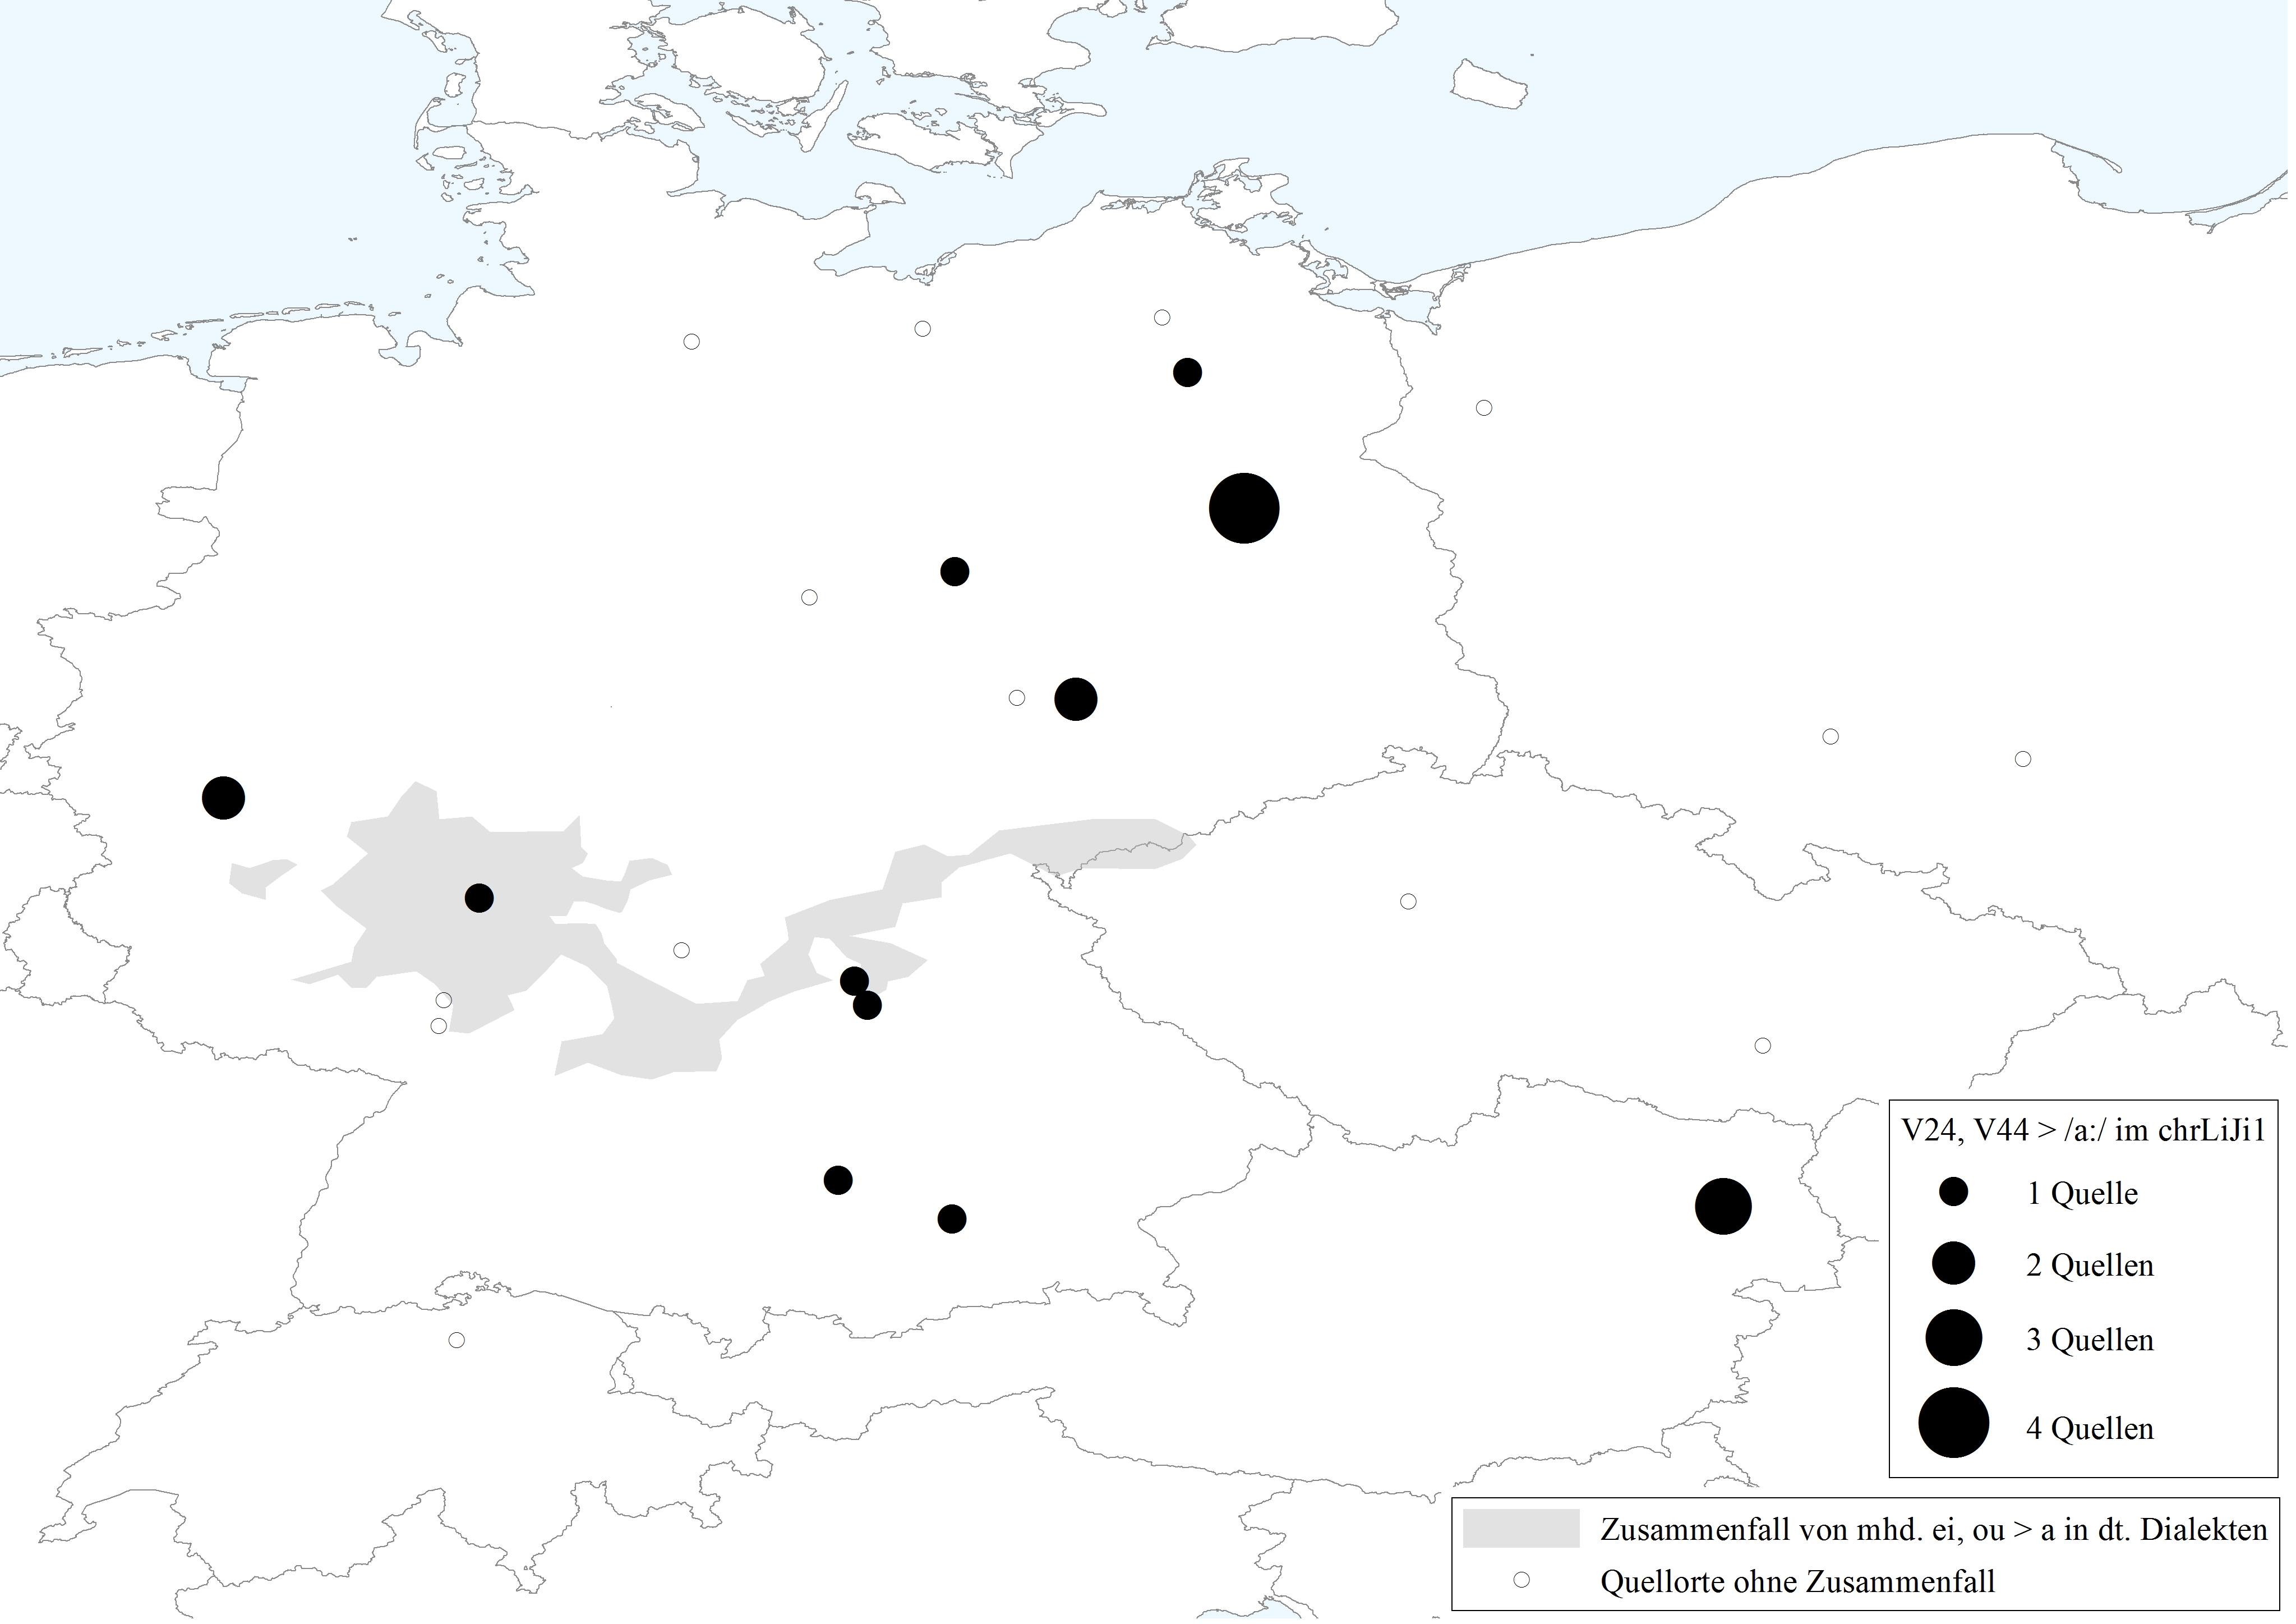
\includegraphics[width=\textwidth]{figures/zusammenfallkarte.png}
		\caption{\label{karteV24V44}  Der \isi{Zusammenfall} von \hai{V24} u. \hai{V44} > /a\textlengthmark/ im \hai{chrLiJi1}}
		\end{figure}

 
Sechs von zehn Quellen des \hai{jüdLiJi1} zeigen den \isi{Zusammenfall} (s. Tabelle \ref{tblV24V44}). Anders als im Fall des \hai{chrLiJi1} sind abweichende Parallelstrategien, wie z.\,B.\, die Monophthongierung von \hai{V24} zu /e\textlengthmark/ neben der zu /a\textlengthmark/, deutlich seltener.\footnote{Welche Quellen neben dem westjiddischen Monophthong welche Markierungen an der Position von \hai{V24} haben, wird in Tabelle \ref{tblV24uedliji} aufgeführt. Im Vergleich zu den Pamphleten tritt der \isi{Zusammenfall} bzw. treten die einzelnen Monophthongierungen insgesamt in den \hai{GuS} deutlich seltener auf. Eine der Quellen, \hai{GuS15}, zeigt sogar weder die Monophthongierung von \hai{V24} noch die von \hai{V44}.}\\ %Im Fall der Manipulation von \hai{V44} weist nur \hai{PDebrecen} eine Markierung als <o>, <oo>, neben der zu <a> auf.} \hai{jüdLiJi1} ist damit deutlich homogener in seinen Markierungen, was auf eine bessere Sprachkompetenz schließen lässt.
 
  \begin{table}
\centering
		\begin{tabular}{lcc}
		\lsptoprule
	\textbf{Quelle} & \textbf{\hai{V24}  > /a\textlengthmark/ }&\textbf{\hai{V44}  > /a\textlengthmark/ } \\ \midrule % horizontale Trennlinie
\hai{GuS1}	&  \checkmark&	\checkmark	\\
\hai{GuS5}	&	\checkmark &	–	\\
\hai{GuS10}	&\checkmark&	–\\
 \hai{GuS15} &	–	& –\\	
\hai{GuS23}	&\checkmark&	\checkmark\\
\hai{PAlsleben}	&	\checkmark&		\checkmark\\
\hai{PBerlin1}	&\checkmark&	–\\
\hai{PBerlin2}	&	\checkmark	&\checkmark \\
\hai{PBreslau}	&\checkmark&\checkmark\\	
\hai{PDebrecen}&	\checkmark&\checkmark	\\	\lspbottomrule
  \end{tabular} 
		 \caption{\hai{V24} und \hai{V44} > /a\textlengthmark/ im \hai{JüdLiJi1}}
		 \label{tblV24V44}
		 \end{table}   
   
\largerpage
 Abschließend lässt sich feststellen, dass die westjiddischen Monophthongierungen von \hai{V24} und \hai{V44} besonders häufig im \hai{{\LiJieins}} auftreten. Eine Nähe zur tatsächlich gesprochenen Sprache ist demnach im \hai{{\LiJieins}} im gesamten 19. Jahrhundert festzustellen. Der für das \hai{{\WJ}} charakteristische \isi{Zusammenfall} von \hai{V24} und \hai{V44} hingegen wird in nur wenigen Quellen vollzogen. Doch immerhin 30\% (16 Texte) des \hai{chrLiJi1}-\isi{Korpus} weisen diesen auf. %Diese Quellen geben damit den westjiddischen \isi{Zusammenfall} von {\mhd} \textit{ei} und \textit{ou} wieder. 
 
 
 
  \section{\hai{V42} (O\textsubscript{2} = mhd. \textit{ô}) }\label{phonV42}
 %  %\noindent
   
   Eine ebenfalls für das \hai{{\WJ}} typische Entwicklung ist die Diphthongierung von \hai{V42} ({\mhd}  \textit{ô}) > /\textopeno \textsubarch{u}/ bzw. /a\textsubarch{u}/ (u.\,a.\, \citealt[167]{Timm1987};\citealt[79]{Herzog1992};\citealt[28]{Beider2010};\ref{bspV42_1}–\ref{bspV42_4}). \cite[58f]{GuggenheimGruenberg1973} kartiert für das westl. \hai{{\SWJ}} ausschließlich die Diphthongierung zu /\textopeno \textsubarch{u}/;\, doch im Elsässer \hai{{\SWJ}} lässt sich auch /a\textsubarch{u}/ finden, wie z.\,B.\, \ref{bspV42_3}. Die Karte Nr. 30 des \hai{LCAAJ} (\citeyear[79]{Herzog1992}) gibt jedoch zur konkreten  Situation der geographischen Verbreitung dieses Phänomens im \hai{{\WJ}} und in den Übergangsgebieten Rätsel auf: Der Karte zufolge war /\textopeno \textsubarch{u}/ im westjiddischen Gebiet weit verbreitet, während /a\textsubarch{u}/ lediglich an einzelnen Orten des westlichen \hai{{\WJ}}, \,%rs Spatium fehlt
   \hai{{\NÜJ}} und \hai{{\SÜJ}} auftrat. An der Karte problematisch ist die quantitative Unausgewogenheit zwischen Flächen (Leitform) und Punkten (singuläre Belege). Zumal angesichts der wenigen Erhebungsorte im \hai{{\WJ}} die Flächenkartierung ist mit Vorsicht zu genießen. Bei genauerer Betrachtung stellt sich heraus, dass /a\textsubarch{u}/  die im westjiddischen Areal weiter verbreitete Variante von \hai{V42} ist und /\textopeno \textsubarch{u}/ hingegen überwiegend in den westjiddischen Varietäten im bairischen, fränkischen, ostfälischen und nordniedersächsischen Raum anzutreffen ist. \,%rs "ist" ergänzen
   Besonders interessant an der Entwicklung von \hai{V42} ist die relativ weit ins \hai{{\WJ}} hineinreichende Form des ostjiddischen Diphthongs /\textopeno \textsubarch{\textsci}/, der laut \hai{LCAAJ} (\citeyear[79]{Herzog1992}) im Jiddischen Berlins, Böhmens und Wiens verbreitet war.    
   
\newpage 
       \eenumsentence{\label{bsp42WJ}
    
 % \item östl. \hai{{\NWJ}}:  \textit{Aufen} \sem{Ofen}  < {\mhd} \textit{oven} \parencite[Bd. 2, Sp. 194]{Lexer1992}\\(Heymann 1909:\,94)   \label{bspV42_1}
   
    \item westl. \hai{{\NWJ}}:  \textit{graus} \sem{groß} 
    < {\mhd} \textit{grôʒ} \parencite[Bd. 1, Sp. 1093]{Lexer1992}  \\
    (\qu{Das verfrühte Schulenrufen} Aurich 1902:\,3. Auftritt [\citealt[132]{Reershemius2007}])   \label{bspV42_1}
    
      \item östl. \hai{{\NWJ}}:  \textit{grauße} \sem{große} 
      \\(Heymann 1909:\,35)   \label{bspV42_1b}
            
    \item \hai{ZWJ}: \RL{גרויזע} \textit{grauze}/\textit{grouze} \sem{große} \\
     (\qu{Die Hochzeit zu Grobsdorf} 1822:\,13)\footnote{Aus dem \hai{ZWJ} sind uns bislang nur authentische Quellen in hebräischen Lettern überliefert. Diese haben den Nachteil, dass man zwar erkennen kann, dass als <\RL{וי}> in der Position von {\mhd} \textit{ô} ein Diphthong steht, jedoch ist es unmöglich zu bestimmen, auf welchen Diphthong genau dieses Digraph verweist. Die Quellen des \hai{{\LiJi}} können hier Daten liefern, die die Quellen jüdischer Autoren bislang nicht bieten können.} \label{bspV42_2}
    
    \item \hai{{\SWJ}}: \textit{grause} \sem{große} \\
    (\qu{S'frömeläs Etziglä} Colmar 1902:\,5) \label{bspV42_3}
    
    \item {\oj}: \RL{גרויס} \textit{groys} \sem{groß} \label{bspV42_4}    
    }
   
 In den deutschen Dialekten gestaltet sich die Verteilung von aus {\mhd} \textit{ô} hervorgegangenen Diphthongen  /\textopeno \textsubarch{u}/, /a\textsubarch{u}/ und  /\textopeno \textsubarch{\textsci}/ folgendermaßen (s.\,a. Karte in Abbildung \ref{karteV42}): /\textopeno \textsubarch{\textsci}/ findet sich nach den Karten des \hai{WA} in keinem großflächigen  Areal (\hai{WA} Karten Nr. 419, 219, 411, 159, 382, 351, 192). Im südlichen Rheinfränkisch, im Oberfränkischen und Nordbairischen und einem kleinen Gebiet um Saarbrücken ist /\textopeno \textsubarch{u}/ verbreitet (\hai{WA} Karten Nr. 419, 219, 411, 159, 382, 192;\,  \citealt[237]{Schirmunski1962}). In einzelnen Lexemen, wie etwa \sem{groß} u. \sem{tot}, reicht dieses Gebiet bis ins Mittelbairische hinein (\hai{WA} Karten Nr. 219, 192). {\mhd} \textit{ô} > /a\textsubarch{u}/ ist in drei größeren Arealen im Schwäbischen, Westfälischen, Schlesischen und einem kleinen Übergangsgebiet zwischen Brandenburgisch und Ostfälisch vorzufinden (\hai{WA} Karten Nr. 419, 219, 411, 159, 382, 351, 192). Ganz anders \,%rs Komma streichen
 als die westjiddischen Entwicklungen aus \hai{V24} und \hai{V44} haben die westjiddischen Diphthonge aus \hai{V42} ihre Entsprechungen in den deutschen Mundarten nun nicht im Mitteldeutschen, sondern im Ober- und Niederdeutschen. Die Situation in den deutschen Dialekten Österreichs, Liechtensteins und der Schweiz, die die Karten des \hai{WA} nicht erfassen, gestaltet sich nach der Karte Nr. 364 des \hai{KDSA} überwiegend so, dass {\mhd} \textit{ô} hier überwiegend erhalten blieb;\, nur im Südbairischen Kärntens und Tirols ist der Diphthong /\textopeno \textsubarch{a}/ verbreitet.

Eine Manipulation von \hai{V42} findet sich im \isi{Korpus} des \hai{chrLiJi1} in 33 Quelltexten. Von diesen verwenden 24 Texte Graphien, die auf den Diphthong /a\textsubarch{u}/ <au> verweisen und acht, welche <ou>, die Leitform des \hai{LCAAJ} (\citealt[79]{Herzog1992}), verwenden. In drei dieser acht Quellen wird  parallel  aber auch /a\textsubarch{u}/ eingesetzt. In fünf Texten findet sich der ostjiddische Diphthong als <oi>, <eu>.\footnote{Diese Form steht in drei Quellen parallel zu <au> und in einer dieser drei zusätzlich parallel zu <ou>.} Eine Quelle (\hai{DG} Wien, 1858) weist einen Beleg für <ä> an der Position von \hai{V42} auf. Auch an diesem Phänomen zeigt sich, dass \hai{chrLiJi1} in Fällen von Manipulation Formen des \hai{{\WJ}} verwendet und nur sehr wenige unplausible Formen (etwa der Beleg aus \hai{DG} Wien, 1858) anzutreffen sind. 


Das Histogramm (s. Abbildung \ref{V42}) zeigt, dass die Verteilung für \hai{V42} als <au> vorwiegend die früheren Quellen bis etwa 1830 dominiert;\, später tritt dies nur mehr vereinzelt auf. \hai{V42} als <ou> und <oi>, <eu> ist auffällig häufig in Quellen zwischen 1835 und 1845 zu finden. Doch die Belege für <ou> ergeben nicht nur in der diachronen Ansicht ein interessantes Bild, sondern clustern auch stark im Raum (vgl.\, Abbildung \ref{karteV42}).

 
  %%%V42Diagramm%\begin{flushleft}	
\begin{figure}
	\begin{tikzpicture}
		\begin{axis}[only marks, width=0.82\textwidth,height=0.2\textheight,
		legend style={at={(1,1)},xshift=+0.2cm, yshift=0cm,anchor=north west,nodes=left},
			%title={Funktionstypen des sp\"aten Westjiddisch},
			xtick={1700, 1725, 1750, 1775, 1800, 1825, 1850, 1875, 1900, 1925, 1950, 1975}, ytick=\empty,
			x tick label style={/pgf/number format/1000 sep=}, 
			y tick label style={/pgf/number format/1000 sep=},
			%extra y ticks={456.1, 1022.4},
			%extra y tick labels={{456,1},{1022,4}},
			extra y tick style={grid=major,
				tick label style={, ,}},
				ymin=0.7,
				ymax=2.7,
			ylabel={Phänomenbelege},
			enlarge x limits=0.03]	
	
			
\addplot [mark=*, black] table [x=jahr, y=au] {figures/V42au.txt};%2.3
\addplot [mark=*, gray] table [x=jahr, y=ou] {figures/V42ou.txt};%2
\addplot [mark=square*, draw=black] table [x=jahr, y=oi] {figures/V42oi.txt};%1.7
\addplot [mark=triangle*, draw=black] table [x=jahr, y=ae] {figures/V42ae.txt};%1.4
\addplot [mark=o, black] table [x=jahr, y=no] {figures/V42no.txt};%1.1

			% Andere Formen a={mark=square*,blue},% b={mark=triangle*,red},% c={mark=o,draw=black}}
						\legend{\hai{V42} als <au>, \hai{V42} als <ou>, \hai{V42}  als <eu>, \hai{V42} als <ä> , unmanipuliert} %macht Legende
		\end{axis}
	\end{tikzpicture}
	\caption{\hai{V42} im \hai{chrLiJi1}}
	\label{V42}	
\end{figure}




Die regionale Verteilung der im \hai{chrLiJi1} vorliegenden Manipulationen von \hai{V42} zeigt ein interessantes Bild (Abbildung \ref{karteV42}). \hai{V42} als <au> streut weiter in das westjiddische und übergangsjiddische Gebiet hinein, als es die Karte des \hai{LCAAJ} \cite[79]{Herzog1992} angibt. Die Leitform des \hai{LCAAJ},  /\textopeno \textsubarch{u}/ <ou>, hingegen findet sich lediglich in einem Areal koterritorial zum Rheinfränkischen und Mittelbairischen, wo in den deutschen Mundarten dieselbe Entwicklung stattgefunden hat. Es ist nicht zu entscheiden, ob uns hier im \hai{chrLiJi1} korrekte Imitationen des örtlichen \hai{{\WJ}} vorliegen, oder ob es sich bei der \isi{Imitation} um Interferenzen mit dem eigenen deutschen Dialekt handelt. An dieser Stelle stößt die Analyse an ihre Grenzen. Es darf angenommen werden, dass /\textopeno \textsubarch{u}/ <ou> der ältere aus \hai{V42} hervorgegangene Diphthong ist, welcher sich in manchen Teilen des Westjiddischen entweder durch den Kontakt zu den deutschen Dialekten oder unabhängig von ihnen zu /a\textsubarch{u}/ weiter entwickelt hat bzw. im Ostjiddischen zu /\textopeno \textsubarch{u}/ wurde. Bislang ist /\textopeno \textsubarch{u}/ lediglich für südwestjiddische und südliche zentralwestjiddische Varietäten belegt (vgl.\, \citealt[58f]{GuggenheimGruenberg1973}).\footnote{Eine punktgenauere Darstellung der Daten, die die Grundlage der Kartierung des \hai{LCAAJ} (\citeyear[79]{Herzog1992}) waren, würde hier evtl.\, von Nutzen sein. Für die älteren Quellen, d.\,h. hebräischschriftliche Texte, sehen wir uns mit dem Problem konfrontiert, dass <\RL{וי}> sowohl für den Diphthong <ou>, als auch für <au> stehen kann. In den Editionen zweier in Quadratschrift geschriebener maskilimischer Quellen von \cite{AptrootGruschka2004} und \cite{copeland1976} werden <\RL{וי}> als <ou> transliteriert, doch ist gerade die Interpretation dieses Graphems äußerst problematisch, da sie ebenso für /a\textsubarch{u}/ oder  /\textopeno \textsubarch{\textsci}/ verwendet wird  (vgl.\, \citealt[167]{Timm1987}). Hinzu kommt, dass die erste Transliteration von Joseph Herz \quji{\RL{אסתר}} (Fürth 1871) durch J. Suhler (Fürth 1871;\, Abdruck in Israelische Kultusgemeinde Fürth 1984–1986) <au> für <\RL{וי}> schreibt. Erst eine erneute, sensitivere Kartierung der Daten des \hai{LCAAJ} würde es erlauben zu entscheiden, wie sich die aus \hai{V42} hervorgegangenen Diphthonge im \hai{{\WJ}} Sprachraum verhalten und wie deren Verhältnis zu den deutschen Dialekten genau aussieht.} Was die Belege für \hai{V42} als <eu>, <oi> betrifft, so muss offen bleiben, ob hier das aus dem \hai{{\OJ}} bekannte Merkmal in die \isi{Imitation} einfloss oder ob es möglicherweise tatsächlich vereinzelt gesprochen wurde, was wiederum der Karte des \hai{LCAAJ} (\citealt[79]{Herzog1992}) zu Folge nicht auszuschließen ist.
 
 
  \begin{figure}
		\centering
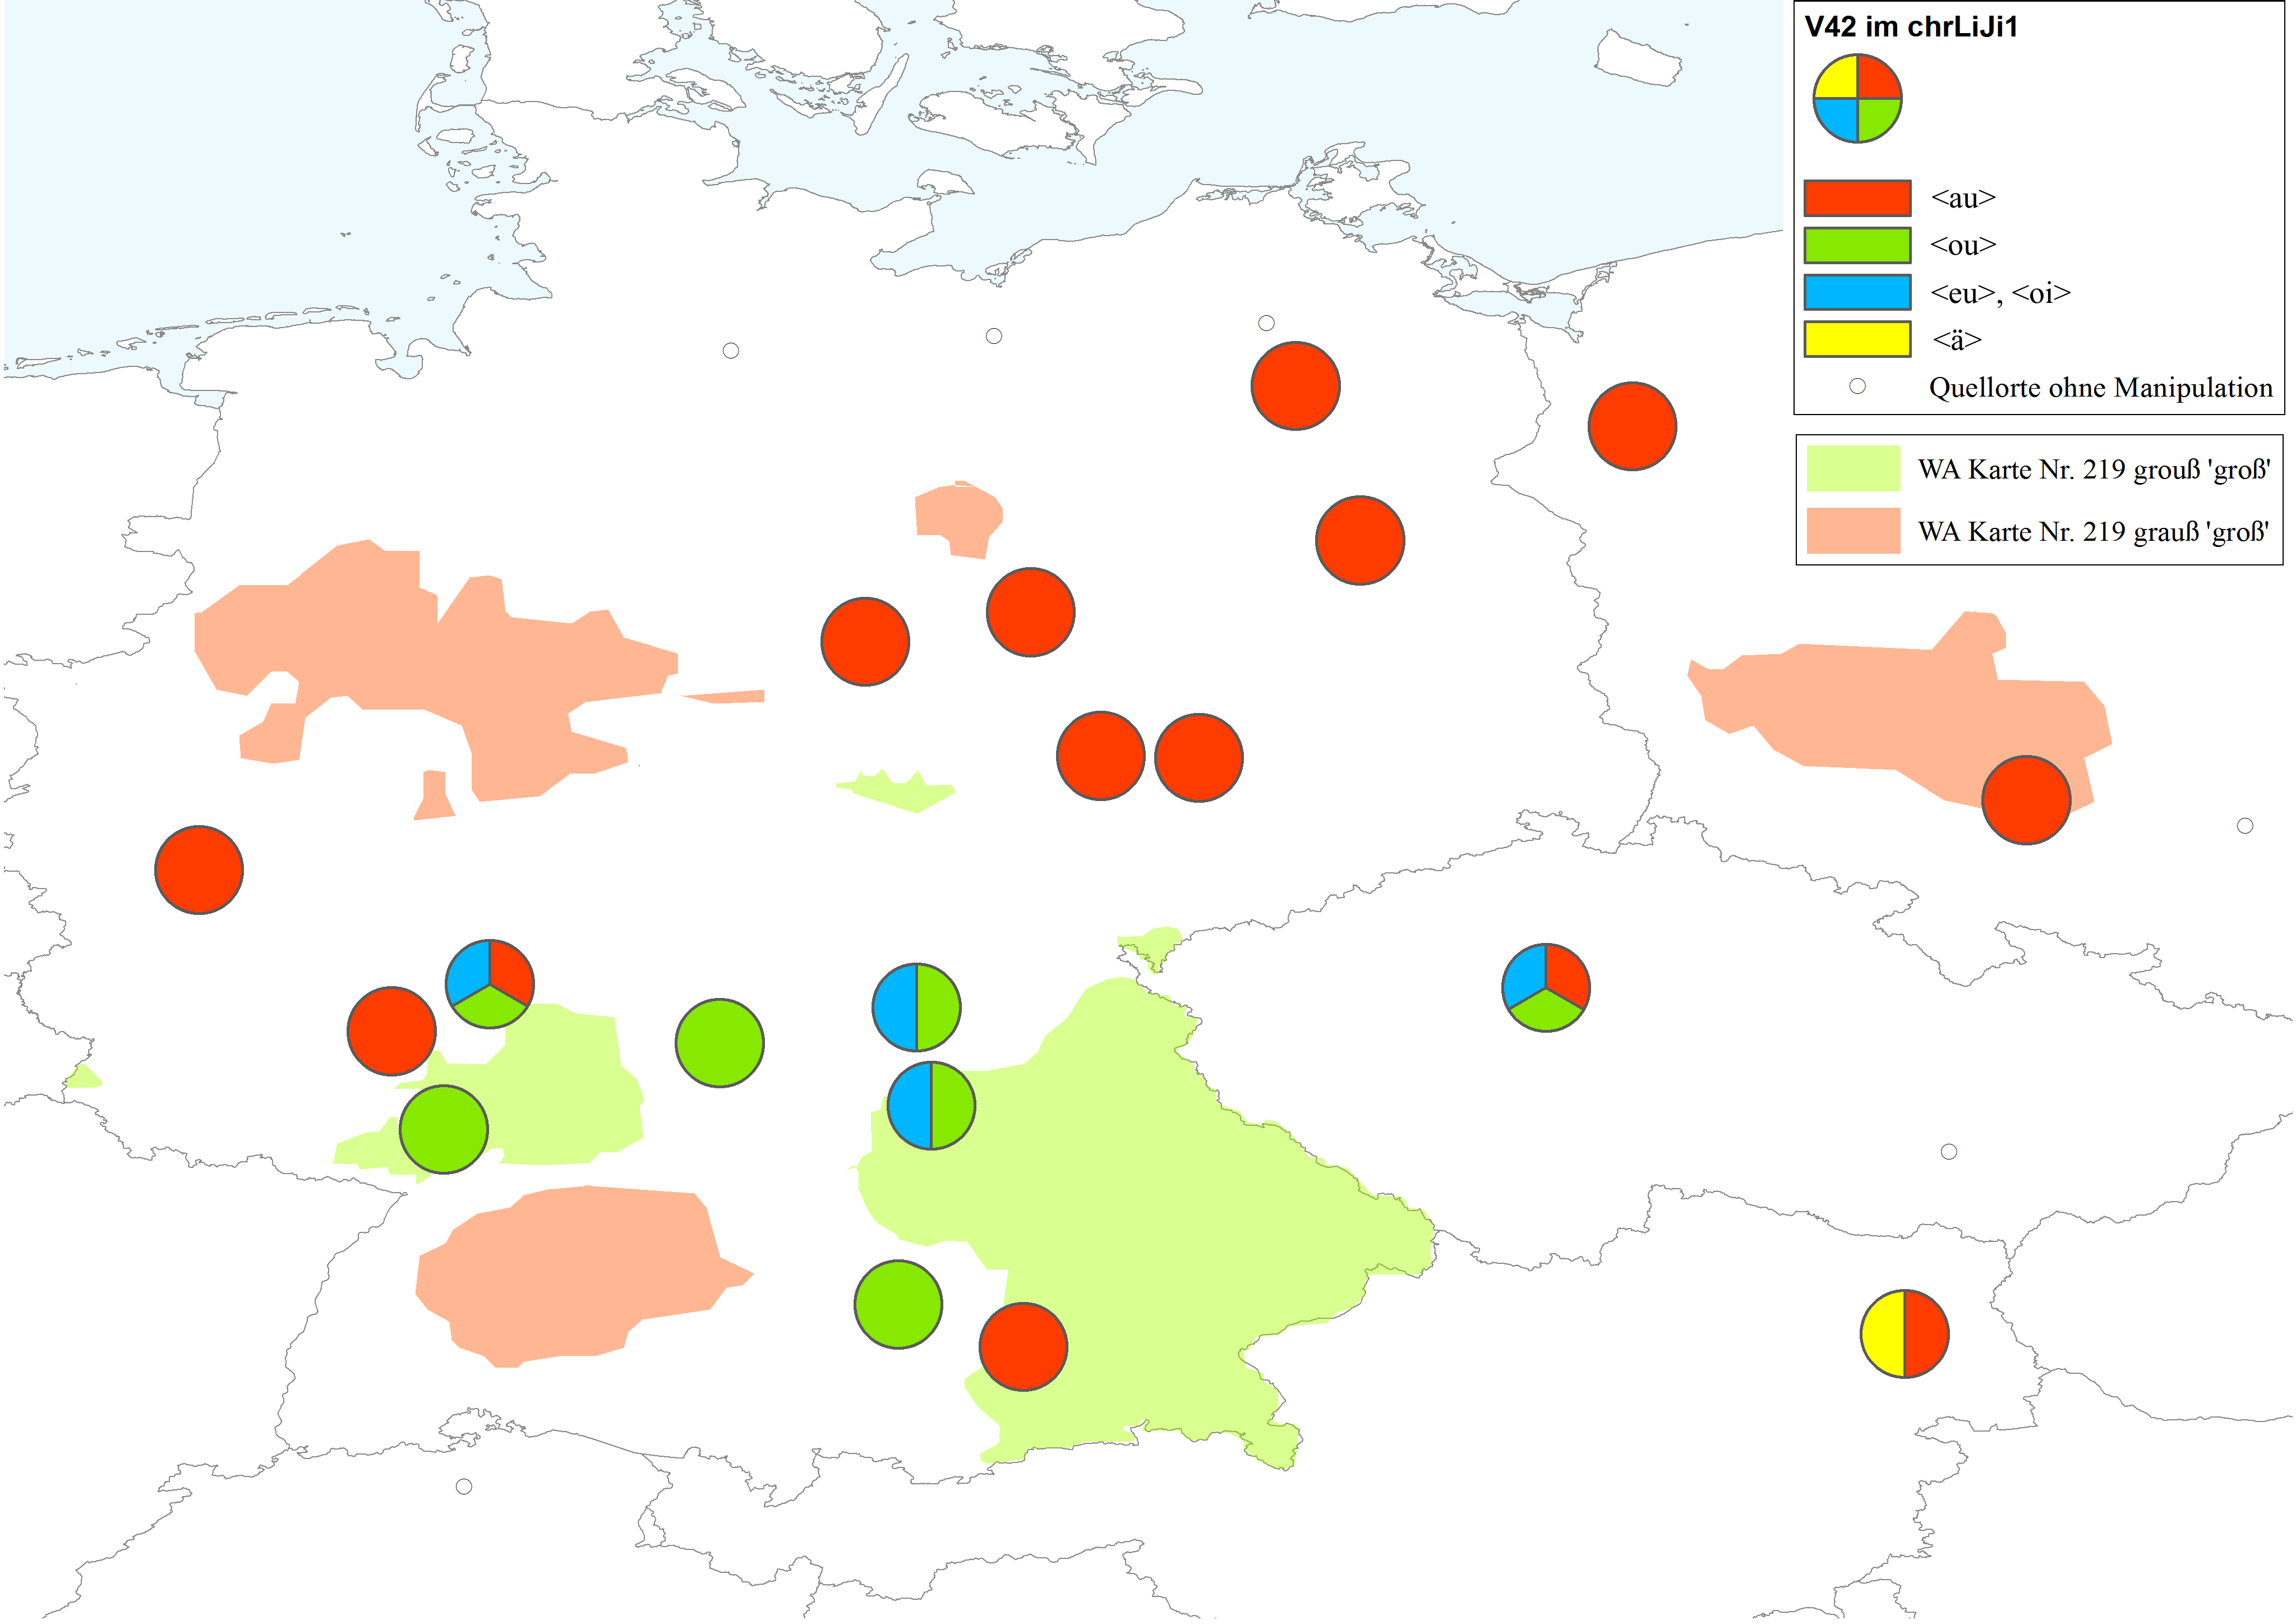
\includegraphics[width=\textwidth]{figures/V42allDSA2.png}
		\caption{\label{karteV42}  \hai{V42} im \hai{chrLiJi1} mit \hai{WA} Karte Nr. 219}
		\end{figure}

 


   
\newpage    
 In sechs der zehn Quellen des \hai{jüdLiJi1} findet sich eine Manipulation von \hai{V42}. In allen Fällen handelt es sich dabei um die Diphthongierung zu  <au>.\footnote{Die entsprechenden Quellen sind \hai{GuS1}, \hai{GuS5}, \hai{PAlsleben}, \hai{PBerlin1}, \hai{PBerlin2} und \hai{PBreslau}.} In \hai{GuS1} findet sich neben dem westjiddischen Diph\-thong auch der ostjiddische Diph\-thong  <oi> belegt. <ou> ist nicht zu finden;\, allerdings stammt auch keine Quelle aus der relevanten Region. Eine nicht in das \isi{Korpus} aufgenommene Quelle des \hai{jüdLiJi1} aus dem fränkischen Raum wäre Jakob Wassermanns autobiographischer Roman \qu{Die Juden von Zirndorf} (1897). Hier finden sich in einem Lexem der Diphthong <ou> belegt: \textit{Jou} (Wassermann [1897] 1996:\,189, 190) \sem{Ja} < {\mhd} \textit{jô} / \textit{jû} \parencite[Bd. 1, Sp. 1481]{Lexer1992}.
 


\noindent Zusammenfassend lässt sich festhalten, dass sich Manipulationen von \hai{V42} in beiden Korpora sehr homogen gestalten: Wenn diese Position manipuliert wird, dann zu einem Diphthong, der die jeweilige Sprachrealität abbildet. Es liegen kaum unplausible Formen der \isi{Imitation} von \hai{V42} vor. 
 

 \section{\hai{V22} (E\textsubscript{2} = {\mhd} \textit{ê}, \textit{œ})}\label{phonV22}
\largerpage[-1]
 %\noindent
 In allen jiddischen Mundarten sind {\mhd} \textit{ê}, \textit{œ} ({\urj} \textit{*\=e\textlengthmark}) zu einem Diphthong zusammengefallen. Im \hai{{\WJ}}, \hai{{\SOJ}} und \hai{{\NOJ}} erfolgte der \isi{Zusammenfall} zu /ɛ\textsubarch{\textsci}/, im \hai{{\ZOJ}} zu /a\textsubarch{\textsci}/ (u.\,a.\, \hai{LCAAJ} \cite[72]{Herzog1992}; \citealt{Timm1987,Beider2010}; erstmals in Boeschenstein 1592 zit. n. \citealt[3]{Mieses1915};\ref{bspv22_1}–\ref{bspv22_1b}). In den deutschen Dialekten ist dieser \isi{Zusammenfall} von {\mhd} \textit{ê} und \textit{œ} > \textit{aj} äußerst selten (\hai{WA} Karten Nr. 461, 167;\, \hai{KDSA} Karten Nr. 378, 382;\, vgl.\, Karte in Abbildung \ref{karteV22}). Im Binnensprachgebiet ist er lediglich in einem kleinen Gebiet des östlichen Rheinfränkischen anzutreffen;\, daneben findet man ihn in Grenz- und Siedlungsmundarten des burgenländischen, böhmischen und mährischen Bairischen. Das größte Areal, in dem diese Entwicklung stattgefunden hat, findet sich im Nordschlesischen. Es fällt auf, dass dieser \isi{Zusammenfall} überwiegend in Kontaktgebieten zu slawischen Sprachen und dem Ungarischen stattgefunden hat.
 
\eenumsentence{ 
 

\item \RL{{ג}\makebox(-0.5,-2.1)[r]{\libertineGlyph{uni05B5}}יהן} \textit{geyhn} \sem{gehen} \\%format!  werden die Diakritika in \RL (.. unter Buchstabe) richtig umgesetzt?
 (\qu{Die Hochzeit zu Grobsdorf} 1822:\,33) < {\mhd} \textit{gên};{\oj} \RL{גיין} \textit{geyn} \label{bspv22_1}

\item \RL{יא}\RL{{ש}\makebox(-0.8,-2.1)[r]{\libertineGlyph{uni05B5}}} \textit{shey} \sem{schön}\\%format!  werden die Diakritika in \RL (.. unter Buchstabe) richtig umgesetzt?
 (\qu{Die Hochzeit zu Grobsdorf} 1822:\,19) < {\mhd} \textit{schœne};{\oj} \RL{שיין} \textit{sheyn} \label{bspv22_1b}

 } 
 
  Von allen 36 Quellen des \hai{chrLiJi1}, die eine Manipulation von \hai{V22} zeigen, wird ein  Diphthong in dieser Position als <ai> (20 Texte), <ei> (neun Texte), <ey> (sechs Texte) oder <ay> (ein Text) verwendet. Die Kartierung der Graphien ergab keine räumlichen Muster. Es ist generell fragwürdig, welchen Zweck die besonderen Graphien des Diphthongs erfüllen sollen;\, scheinbar wurde der Diphthong als vom standarddeutschen /a\textsubarch{\textsci}/ <ei> abweichend dargestellt. Es ist aber auch möglich, dass durch die Graphie als <ai> ein \isi{phonetisch} geeigneteres Graphem des Diphthongs /a\textsubarch{\textsci}/ verwendet wurde, als das im deutschen Standard übliche <ei>, welches eine größere graphem-phonematische Distanz zum tatsächlichen Laut aufweist. Die unterschiedliche Schreibweise in \qu{Die Hochzeit zu Grobsdorf} der Vokale \hai{V22} (als <\RL{י}> und <\RL{{\,}\makebox(-0.3,0)[r]{\libertineGlyph{uni05B5}}}>, %format!  werden die Diakritika in \RL (.. unter Buchstabe) richtig umgesetzt?
  s. Bsp.  \ref{bspv22_1}–\ref{bspv22_1b}, S.\, \pageref{bspv22_1}) und \hai{V34}  (als <\RL{יי}>  (\ref{grobbspv34_1})–(\ref{grobbspv34_2}) S.\, \pageref{grobbspv34_1}) spricht allerdings stark dafür, eine unterschiedliche Aussprache der beiden Vokale auch im Westjiddischen anzunehmen. Da aber im Fall des \hai{{\LiJi}} nicht zu entscheiden ist, welcher Laut sich tatsächlich hinter welchem Graphem verbergen soll (und tatsächlich auch nicht, wie <ei> im 19. Jahrhundert von Sprechern des Deutschen realisiert wurde), wird im folgenden /ɛ\textsubarch{\textsci}/ als der im \hai{{\WJ}} gebräuchliche Diphthong idealisierend gesetzt. 
 

Für die Graphie interessant sind die Belege aus dem kleineren \isi{Korpus}: Im \hai{jüdLiJi1} zeigen acht der zehn Quellen eine Manipulation von \hai{V22} als <ei>.\footnote{Dies betrifft die Texte \hai{GuS1,5,15,23}, \hai{PAlsleben}, \hai{PBerlin1}, \hai{PBerlin2} und \hai{PBreslau}. Die Texte \hai{GuS23}, \hai{PAlsleben} u. \hai{PBerlin2} zeigen nur Belege für den Diphthong < {\mhd}  \textit{ê}. Die  übrigen fünf Quellen haben den \isi{Zusammenfall} belegt.} Alle dieser Texte setzen <ei>, also das standarddeutsche Graphem. 


Es lässt sich festhalten, dass die orthographischen Strategien im \hai{jüdLiJi1} insgesamt näher am gesprochenen Laut /ɛ\textsubarch{\textsci}/ sind als die des \hai{chrLiJi1}.
 
 Die Hauptbelege einer Manipulation von \hai{V22} in beiden Korpora treten am Kennlexem \sem{wehe} auf (vgl.\, Unterabschnitt \ref{interjektionen}), welches die Belegzahlen zu diesem Phänomen in die Höhe treibt. Der \isi{Zusammenfall} selbst ist im \hai{chrLiJi1} nur in neun Texten belegt,\footnote{Die entsprechenden Quellen sind \hai{AD} (Leipzig, 1846), \hai{AJ} (Berlin, 1825), \hai{AK} (Zürich, 1948), \hai{DW} (Wien, 1773), \hai{MV} (Berlin, 1862), \hai{NW} (Berlin, 1804), \hai{SV} (München, 1890), \hai{TH} (Merseburg, 1820) u. \hai{VD} (Frankfurt, 1916).} eine Quelle manipuliert nur {\mhd} \textit{œ},\footnote{Es handelt sich um die Quelle \hai{WA} (Magdeburg, 1802).} die übrigen 23 Quellen manipulieren lediglich {\mhd} \textit{ê}.  Das Histogramm in Abbildung \ref{V22zusammen} zeigt, dass der \isi{Zusammenfall} v.\,a.\, in Quellen des frühen 19. Jahrhunderts zu finden ist, aber auch in den späteren Quellen  auftaucht.

  %%%V22Diagramm%\begin{flushleft}	
\begin{figure}
	\begin{tikzpicture}
		\begin{axis}[only marks, width=0.82\textwidth,height=0.2\textheight, 
		legend style={at={(1,1)},xshift=+0.2cm, yshift=-0.04cm,anchor=north west,nodes=left}, 
			%title={Funktionstypen des sp\"aten Westjiddisch},
			xtick={1700, 1725, 1750, 1775, 1800, 1825, 1850, 1875, 1900, 1925, 1950, 1975}, ytick=\empty,
			x tick label style={/pgf/number format/1000 sep=}, 
			y tick label style={/pgf/number format/1000 sep=},
			%extra y ticks={456.1, 1022.4},
			%extra y tick labels={{456,1},{1022,4}},
			extra y tick style={grid=major,
				tick label style={, ,}},
				ymin=0.7,
				ymax=2.7,
			ylabel={Phänomenbelege},
			enlarge x limits=0.03]				
\addplot [mark=*, black] table [x=jahr, y=zusammenfall] {figures/V22zusammenfall.txt};%2.1
\addplot [mark=*, gray] table [x=jahr, y=nur_e] {figures/V22nur_e.txt};%1.7
\addplot [mark=square*, draw=black]  table [x=jahr, y=nur_oe] {figures/V22nur_oe.txt};%1.3
\addplot [mark=o, black] table [x=jahr, y=no] {figures/V22no2.txt};%1.1
\legend{{}{\mhd} \textit{ê}, \textit{œ} als <ei>, {\mhd} \textit{ê} als <ei>,  {\mhd} \textit{œ} als <ei>,  unmanipuliert} %macht Legende
% Andere Formen a={mark=square*,blue},% b={mark=triangle*,red},% c={mark=o,draw=black}}
		\end{axis}
	\end{tikzpicture}
	\caption{Der \isi{Zusammenfall} von \hai{V22} im \hai{chrLiJi1}}
	\label{V22zusammen}	
\end{figure}

 
 
 Die räumliche Verteilung zeigt, dass bei diesem Phänomen keine Beeinflussung durch deutsche Dialekte im \hai{chrLiJi1} vorliegt (Karte in Abbildung \ref{karteV22}). Die Regionen, in denen der \isi{Zusammenfall} von {\mhd} \textit{ê}, \textit{œ} > /ɛ\textsubarch{\textsci}/ in den deutschen Dialekten stattfand, sind im Projektsample des \hai{chrLiJi1} kaum vertreten. Einzige Ausnahme bildet Wien, wo der \isi{Zusammenfall} sowohl im \isi{Korpus} als auch in der näheren Umgebung im deutschen Dialekt gegeben ist. Durchaus interessant sind die Raumbilder der Karte \ref{karteV22} dennoch. Allem Anschein nach sind Diphthongierungen, die zu einem \isi{Zusammenfall} von {\mhd} \textit{ê}, \textit{œ} > /ɛ\textsubarch{\textsci}/ führen, auch in den deutschen Mundarten deutlich aneinander gebunden. Die Diphthongierung von {\mhd}\textit{œ} findet selten ohne die von {\mhd} \textit{ê} statt (und umgekehrt), was darauf schließen lässt, dass der \isi{Zusammenfall} nicht auf direktem Weg durch die Diphthongierung erfolgte, sondern die \isi{Entrundung} von \textit{œ} > \textit{ê}  bereits zum \isi{Zusammenfall} mit {\mhd} \textit{ê} geführt hat. Wie auch im \isi{Zusammenfall} von {\mhd} \textit{ei} und \textit{ou} > /a\textlengthmark/ (Abbildung \ref{dteiou}) entsprechen (west-)jiddische Entwicklungen damit Strukturen, wie sie auch in den deutschen Dialekten vorherrschen. 
 
 
  \begin{figure}
		\centering
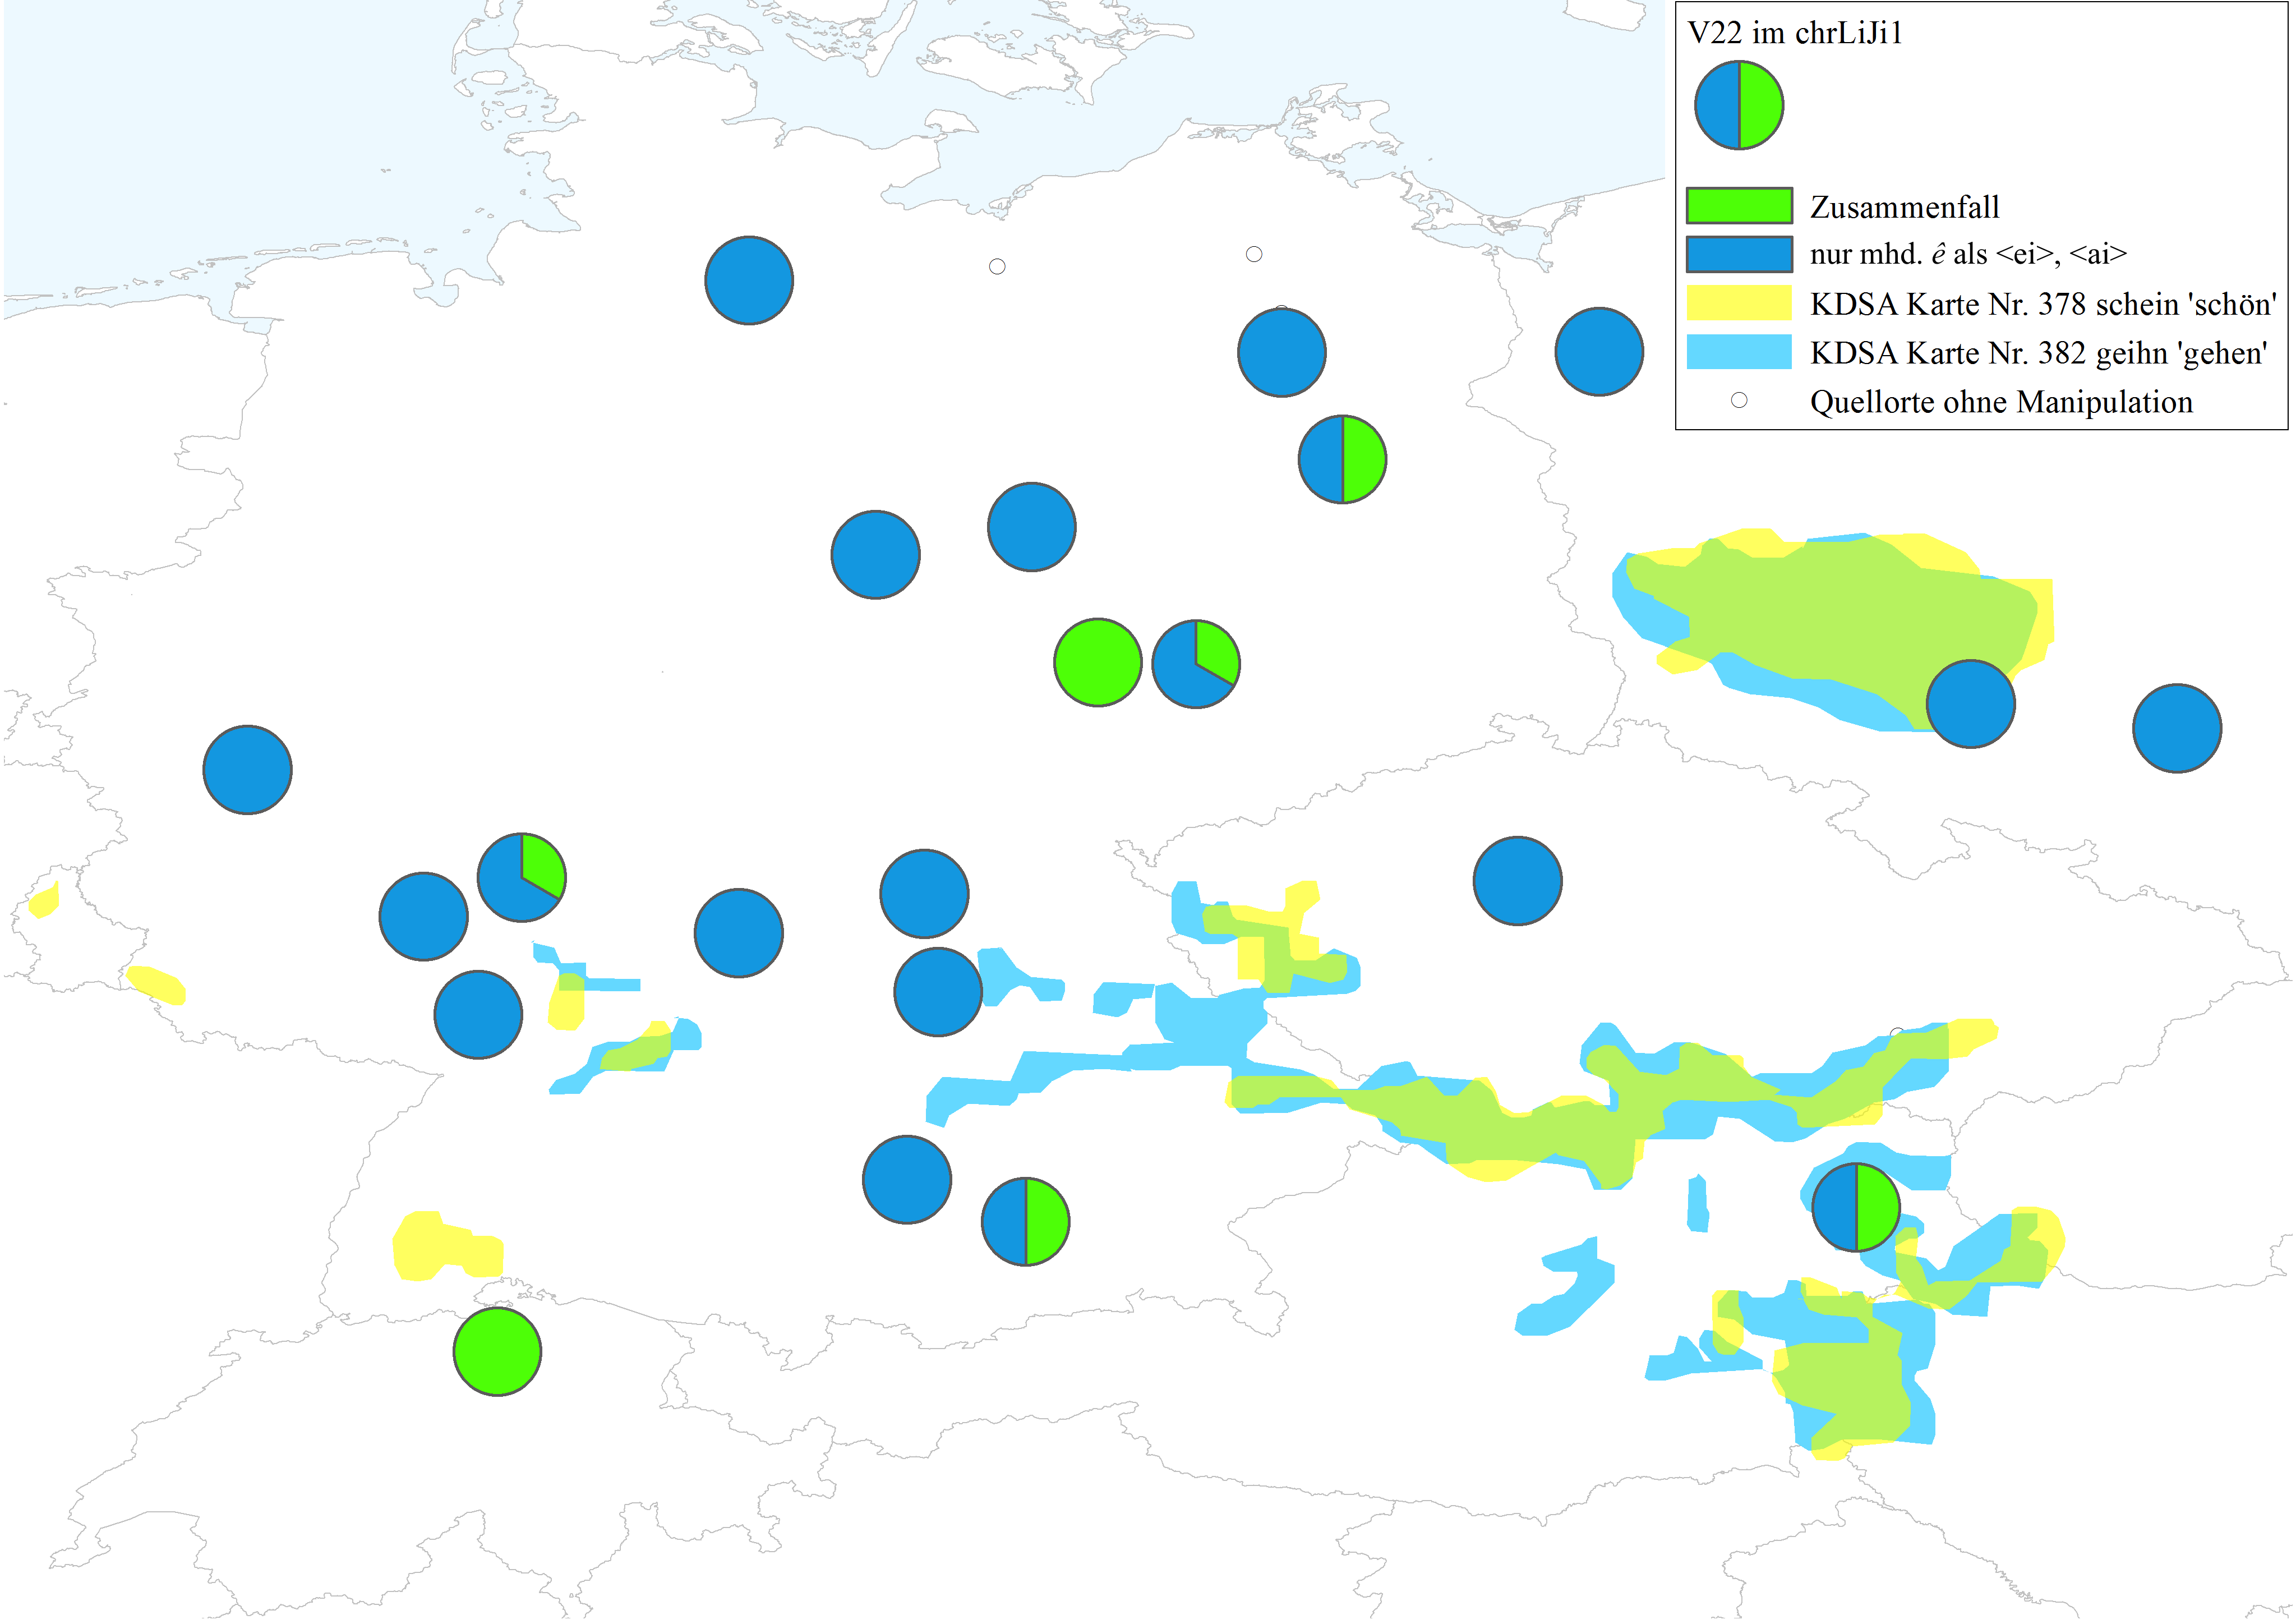
\includegraphics[width=\textwidth]{figures/V22zusammenfall2.png}
		\caption{\label{karteV22}  \hai{V22} im \hai{chrLiJi1} mit \hai{KDSA} Karten Nr. 378, 382}
		\end{figure}

 



 
 
 \section{\hai{V34} (I\textsubscript{4} = {\mhd} \textit{iu}, \textit{î})}\label{phonV35}

{\MHD} \textit{iu} und \textit{î} sind in den meisten west- und ostjiddischen Dialekten zu /a\textsubarch{\textsci}/ zusammengefallen (\hai{LCAAJ} \citealt[77]{Herzog1992};\citealt[206]{Timm1987} (\ref{grobbspv34_1})--(\ref{grobbspv34_2}), s.\,a. (\ref{bspV34_1})–(\ref{bspV34_4}) S.\, \pageref{bspV34_1}). Im \hai{{\ZOJ}}, östlichen \hai{{\SÜJ}} und südlichen \hai{{\SOJ}} ist dieser Diphthong zu /a\textlengthmark/, bzw. /a/ im \hai{{\SOJ}} monophthongiert worden (\citealt[77]{Herzog1992};\citealt[206]{Timm1987};s. Unterabschnitt \ref{hyperV24}). Den westjiddischen Diphthong /a\textsubarch{\textsci}/ < {\mhd} \textit{iu} findet man in den deutschen Dialekten sehr weit verbreitet. Er deckt besonders große Teile des östlichen Sprachgebiets ab (\hai{WA} Karten Nr. 319, 463, 497, 519, 542;\, \hai{KDSA} Karte Nr. 410). Eine Entwicklung von {\mhd}  \textit{iu} > /a\textsubarch{\textsci}/ ist in den oberdeutschen Dialekten keine Seltenheit. Dort ist der Diphthong, mit Ausnahme des Alemannischen,\footnote{Schwäbisch, was hier nicht im eigentlichen Sinn als Alemannisch verstanden wird, da es u.\,a.\, die sog. \quein{nhd. Diphthongierung u. Monophthongierung} mitgemacht hat, zeigt ebenfalls {\mhd}  \textit{iu} > /a\textsubarch{\textsci}/.} in großen Teilen des Ostmittel- und Ostniederdeutschen, sowie im Rhein-, Mosel- und Niederfränkischen und in nordniederdeutschen Übergangsgebieten belegt (vgl.\,\hai{WA} Karten Nr. 463, 519, 196).



\eenumsentence{
 

\item \RL{נייא} \textit{ney} \sem{neu} \\
(\qu{Die Hochzeit zu Grobsdorf} 1822:\,21) 
\\ < {\mhd} \textit{niuwe};vgl.\, {\oj} \RL{נ{יי}\makebox(-1.5,-3.5)[r]{\libertineGlyph{uni207B}}} \textit{nay} \label{grobbspv34_1}

\item \RL{בראנטעווייא} \textit{brantwey} \sem{Branntwein}\\
 (\qu{Die Hochzeit zu Grobsdorf} 1822:\,7) \\
 < {\mhd} \textit{wî};vgl.\, {\oj} \RL{וו{יי}\makebox(-1.5,-3.5)[r]{\libertineGlyph{uni207B}}ן} \textit{vayn}\label{grobbspv34_2}
 
 }



Die Diphthongierung von {\mhd} \textit{î} > /a\textsubarch{\textsci}/ haben im Zuge der
\qu{neuhochdeutschen Diphthongierung} zwischen dem 12. und 16. Jahrhundert neben dem Jiddischen alle hochdeutschen Dialekte (mit Ausnahme des Alemannischen) mitgemacht (\citealt[146–149]{Koenig1978};\citealt[14–18]{Timm1987}). Dieser Diphthong ging auch in die Leitvarietät über und ist damit Bestandteil der neuhochdeutschen Standardsprache. Eine Weiterentwicklung von {\mhd} \textit{î} > /a\textsubarch{\textsci}/, wie z.\,B.\, die Rückmonophthongierung im \hai{{\ZOJ}}, hat in kaum einem deutschen Dialekt stattgefunden (vgl.\, \hai{WA} Karten Nr. 15, 176, 180). Da die westjiddische Form dem Schriftdeutschen entspricht, kann nicht überprüft werden, ob Belege für <ei>, <ai> an der Position von {\mhd} \textit{î} in \isi{Analogie} zum Jiddischen gesetzt wurden oder nicht;\, hier ist also keine Manipulation erkennbar. Es darf jedoch als besonderer Hinweis auf die korrekte Orientierung am Jiddischen interpretiert werden, dass im \hai{{\LiJi}} {\mhd} \textit{î} in keinem Fall Formen annimmt, die nicht einer jiddischen Varietät entsprechen (s. Unterabschnitt \ref{hyperV24}). 

Damit ist \hai{V34} für das \hai{{\LiJi}} nur an der Position von {\mhd} \textit{iu} relevant. 27 Quellen des \hai{chrLiJi1}-\isi{Korpus} zeigen eine Manipulation in dieser Position. In 16 Belegen findet sich <ai>, in zehn Texten <ei> (in drei Texten liegen beide Graphien parallel vor).\footnote{Dabei handelt es sich um die Quellen \hai{SV} (München, 1890), \hai{TH} (Merseburg, 1820) u. \hai{VD} (Frankfurt, 1916).} Auch hier lassen sich damit alle Manipulationen auf die tatsächliche Sprachrealität zurückführen. Eine Manipulation von \hai{V34} tritt erst ab 1800 wirklich in Erscheinung (Abbildung \ref{V34}).  Ab 1880 ist \hai{V34} in allen Quellen manipuliert.
 
  %%%V34Diagramm%\begin{flushleft}	
\begin{figure}
	\begin{tikzpicture}
		\begin{axis}[only marks, width=0.82\textwidth,height=0.2\textheight,
		legend style={at={(1,1)},xshift=+0.2cm, yshift=-0.44cm,anchor=north west,nodes=left},
			%title={Funktionstypen des sp\"aten Westjiddisch},
			xtick={1700, 1725, 1750, 1775, 1800, 1825, 1850, 1875, 1900, 1925, 1950, 1975}, ytick=\empty,
			x tick label style={/pgf/number format/1000 sep=}, 
			y tick label style={/pgf/number format/1000 sep=},
			%extra y ticks={456.1, 1022.4},
			%extra y tick labels={{456,1},{1022,4}},
			extra y tick style={grid=major,
				tick label style={, ,}},
				ymin=0.7,
				ymax=2.9,
			ylabel={Phänomenbelege},
			enlarge x limits=0.03]	
	
			
\addplot [mark=*, black] table [x=jahr, y=ai] {figures/V34ai.txt};%2.3
\addplot [mark=*, gray] table [x=jahr, y=ei] {figures/V34ei.txt};%1.8
\addplot [mark=o, black] table [x=jahr, y=no] {figures/V34no.txt};%1.3


 

			% Andere Formen a={mark=square*,blue},% b={mark=triangle*,red},% c={mark=o,draw=black}}
						\legend{\hai{V34} als <ai>, \hai{V34} als <ei>, unmanipuliert} %macht Legende
		\end{axis}
	\end{tikzpicture}
	\caption{\hai{V34} ({\mhd} \textit{iu}) im \hai{chrLiJi1}}
	\label{V34}	
\end{figure}

 
 
 Auch im Fall vom westjiddischen Diphthong < \hai{V34} ist die Graphie ähnlich irreführend, wie es im Fall des Diphthongs < \hai{V22} bereits angesprochen wurde (vgl.\, Abschnitt \ref{phonV22}). Ein Vergleich zwischen der Verwendung von <ai>, <ay> vs. <ei>, <ey> im \hai{V34}- vs. \hai{V22}-Kontext ergibt, dass keine Regelmäßigkeit zu erkennen ist. Alle vier Grapheme können so für die Laute /ɛ\textsubarch{\textsci}/ und /a\textsubarch{\textsci}/ stehen. 
 
 Abbildung \ref{karteV34} zeigt die räumliche Verteilung von Manipulationen im \hai{V34}-Kontext. Da der westjiddische Diphthong auch in Quellorten auftritt, an denen in den deutschen Dialekten keine entsprechende Entwicklung stattgefunden hat, kann man (zumindest an diesen Orten mit relativer Gewissheit) davon ausgehen, dass die Formen im \hai{chrLiJi1} keine Reflexe aus den deutschen Mundarten sind, sondern spezifisch als jiddische Form eingesetzt werden.
 
 
 \begin{figure}
		\centering
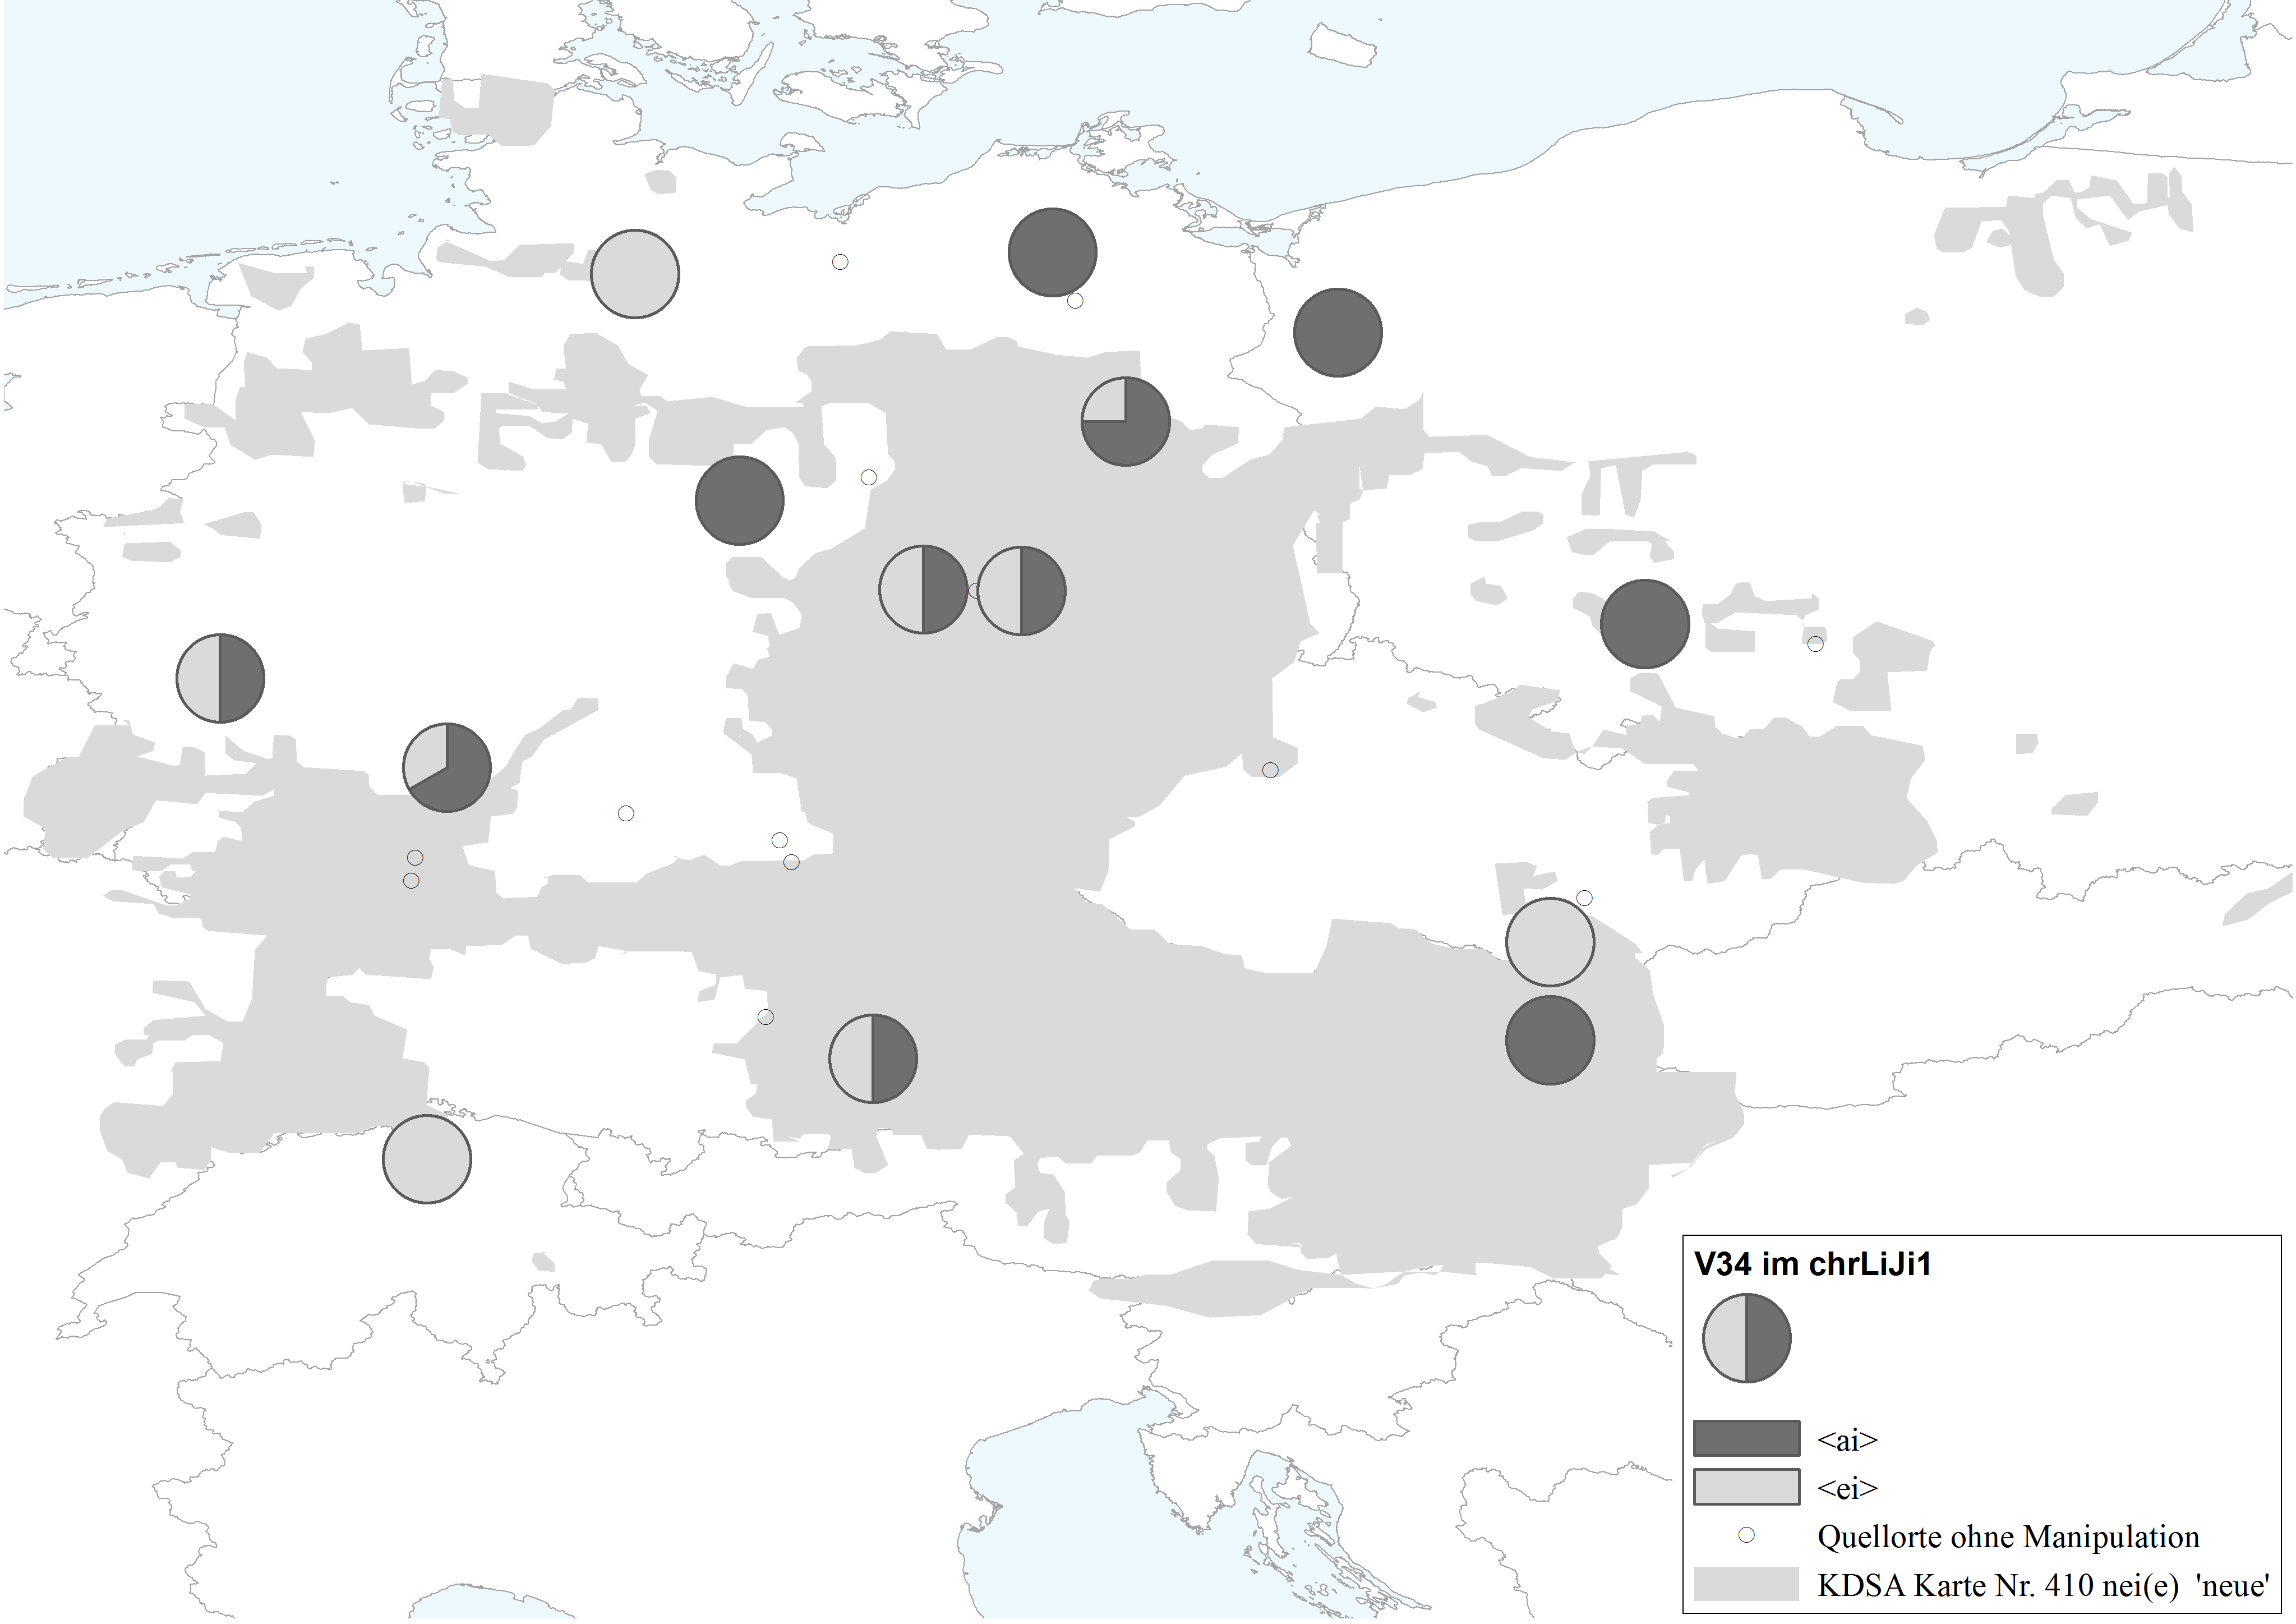
\includegraphics[width=\textwidth]{figures/v34karte2.png}
		\caption{\label{karteV34}  \hai{V34} im \hai{chrLiJi1} mit \hai{KDSA} Karte Nr. 410}
		\end{figure}

 
 
\largerpage
 Das \hai{jüdLiJi1} zeigt in acht Quellen den jiddischen Diphthong;\, in fünf von acht Fällen liegt die Schreibung <ei> vor und in drei von acht die mittels <ai>.\footnote{<ei> findet sich in \hai{GuS1,5,10}, \hai{PBreslau} u. \hai{PDebrecen};<ai> findet sich in \hai{GuS23}, \hai{PBerlin2} u. \hai{PAlsleben}.}\\
 
   \section{/a/ > /o/ (\textit{a}-Ver\-dumpf\-ung)}\label{phonV1213}

Die \isi{Rundung} und Hebung von \textit{a}>\textit{o} wird hier vereinfachend als \qu{\textit{a}-Verdumpfung} bezeichnet. Im \hai{{\OJ}} fiel \hai{V12} ({\urj} *\textit{\=\textopeno\textlengthmark, A\textsubscript{2}}, = {\mhd} \textit{â}, {\oj} \RL{י{א\makebox(-1.25,-1.25)[r]{\libertineGlyph{uni05B8}}}ר} \textit{yor} \sem{Jahr}) und \hai{V13} ({\urj} *\textit{a} in offener Tonsilbe,  A\textsubscript{3}, = {\mhd} \textit{a}/\textit{â}, {\oj} \RL{של{א\makebox(-1.25,-1.25)[r]{\libertineGlyph{uni05B8}}}גן} \textit{shlogn} \sem{schlagen}) zu /\textopeno\textlengthmark/ zusammen und wurde im \hai{{\ZOJ}} zu /u\textlengthmark/ gehoben (\citealt[93–121]{Timm1987};\citealt[186f]{Bin-Nun1973}). Im \hai{{\WJ}} hingegen wurde lediglich \hai{V12} verdumpft;\, \hai{V13}, also *\textit{a} in offener Tonsilbe, blieb unverändert \parencite{Beider2010}. Abbildung \ref{karteV1213} zeigt, dass auch in den deutschen Dialekten die Ver\-dumpf\-ung im \hai{V13}-Kontext weniger präsent ist als die im \hai{V12}-Kontext und dass die Verdumpfung vorrangig in den östlichen Dialekten im Kontaktbereich zu slawischen (und finno-ugrischen) Sprachen stattgefunden hat. Dies könnte u.\,U. eine Erklärung dafür liefern, wieso diese Verdumpfung nur im \hai{{\OJ}} stattgefunden hat. Andererseits ist die Situation in den westjiddischen Varietäten alles andere als klar, denn bislang ist lediglich das \hai{{\SWJ}} der Schweiz ausreichend beschrieben worden (\citealt{GuggenheimGruenberg1973,Beider2010}).\footnote{Der \hai{LCAAJ} kartiert \hai{V13} nur am Beispiel eines {\hebr} Lexems (\citealt[68]{Herzog1992}), was was für die Situation der Germanismen wenig aussagekräftig ist.} 
Bislang fehlen Detailanalysen zu weiteren westjiddischen Dialekträumen.

 
Ein weiteres Problem, das sich bei diesem Phänomen ergibt, betrifft die Bestimmung eines Vokals als einem aus \hai{V12} hervorgegangenem. Die Analyse von \hai{V12} im \hai{{\WJ}} führte in den bisherigen Arbeiten m.\,E. oft zu vorschnellen Schlüssen, da ein zu starkes Gewicht auf die gemeinsame Genese von Ost- und \ili{Westjiddisch} gelegt wurde. Die Karten des \hai{LCAAJ} (\citeyear[67]{Herzog1992}) und \citeauthor{GuggenheimGruenberg1973}s (\citeyear[60–64]{GuggenheimGruenberg1973}) geben an, dass \hai{V12} im westlichen Teil des \hai{{\WJ}} als /\textopeno \textsubarch{u}/ oder /a\textsubarch{u}/ und im \hai{{\SÜJ}},
 im westl. \hai{{\SWJ}} als /\textopeno \textsubarch{\textsci}/ realisiert wurde (s.\,a. \citealt{Beider2010}). Im \hai{{\WJ}} beträfe dies nach den Daten des \hai{LCAAJ}s ohnehin nur einzelne (leider nicht näher angegebene) Wörter hebräischen Ursprungs. Für das \hai{{\SÜJ}} und das westl. \hai{{\SWJ}} sind zwar die einzelnen, überwiegend germanischstämmigen Lexeme gegeben (vgl.\, \citealt{GuggenheimGruenberg1973}), doch bei diesen ist der {\mhd} Vokal nicht gänzlich geklärt. So werden etwa die Formen für \RL{דוי}  \sem{hier, da} und \RL{של{א\makebox(-1.25,-1.25)[r]{\libertineGlyph{uni05B8}}}פן}  \sem{schlafen} angegeben. Diese Lexeme sind für das {\MHD} aber sowohl als \textit{dô}, \textit{slôfen} wie auch als \textit{dâ}, \textit{slâfen} belegt \parencite[Bd. 1, Sp. 445]{Lexer1992}. Der Diphthong /\textopeno \textsubarch{u}/, bzw. /\textopeno \textsubarch{\textsci}/ im \hai{{\SÜJ}}, kann damit aus \hai{V42} (= {\mhd} \textit{ô}) hervorgegangen sein, bei welchem eine solche Diphthongierung im \hai{{\WJ}} stattgefunden hat (vgl.\, Abschnitt \ref{phonV42};s.\,a. \citealt[188]{Bin-Nun1973}). Dieser kann wiederum aus einer Verdumpfung von \textit{â} zustande gekommen sein.\footnote{Einige solcher Lexeme, die nach den Entwicklungen von \hai{V42} diphthongiert wurden (z.\,B.\, \sem{da}, \sem{ja}), wurden in dieser Arbeit auch als ein solches Phänomen analysiert und entsprechend nicht in die Daten zur \textit{a}-Verdumpfung aufgenommen (vgl.\, Abschnitt \ref{phonV42}). Nach \cite[60f]{GuggenheimGruenberg1973} besteht im westl. \hai{{\SWJ}} sogar gar keine Unterscheidung mehr zwischen \hai{V13}, \hai{V12} und \hai{V42}. Diese sind, zumindest in den kartierten Lexemen, unter dem Diphthong aus \hai{V42} zusammengefallen. Sie kartiert die Lexeme \sem{schlafen}, \sem{raten}, \sem{fragen} (> {\urj} *\textit{a} in offener Tonsilbe = \hai{V13} gemeinsam mit \sem{mal}, \sem{da} (> \hai{V12} bzw. \hai{V42}) als < {\mhd} \textit{â}. Siehe hierzu auch \cite[115]{Timm1987}. Um aber die Situation der Verdumpfung und Diphthongierung im \hai{{\WJ}} genau erfassen zu können, bedarf es einer Detailanalyse, die diese Arbeit nicht leisten kann.} Eine solche Vermutung müsste allerdings erklären, wieso im \hai{{\OJ}} eine Diphthongierung nach dem Muster von \hai{V42} am verdumpften \hai{V12} nicht stattgefunden hat. Dieses Phänomen wäre also neben der Monophthongierung von \hai{V24} und \hai{V44} eine phonologische Entwicklung, in der sich \hai{{\WJ}} und \hai{{\OJ}} auseinander entwickelt haben. Darüber hinaus spiegelt die Situation der Vokale \hai{V11}, \hai{V12}, \hai{V13} und \hai{V42} in den germanischen Lexemen des Jiddischen den Umstand wider, dass es bereits im {\MHD} (regionale) Variation bei der Verdumpfung von \textit{a}-Phonemen gegeben hat. In der deutschen Sprachgeschichte ist die Verdumpfung \,%rs die 
von {\mhd} \textit{â} (einschließlich \textit{a} in offener Tonsilbe) ab dem 12. Jahrhundert in der Schriftsprache zunächst im Bairischen nachweisbar und greift im 13. und 14. Jahrhundert auf das Niederalemannische und die mitteldeutschen Dialekte  über (\citealt[212]{Schirmunski1962}; \citealt[§48]{Paul2007};\citealt[§L14]{Ebert1993}).
\largerpage[-1]
Verdumpfungen \qu{treten in bestimmter konsonantischer Umgebung ein, ohne dass sich daraus eine feste Regel ableiten lässt} \parencite[§48]{Paul2007}. Damit ist  auch die Entwicklung im Deutschen nicht auf eine einfache Formel zu bringen. Sie ist in den modernen deutschen Dialekten mit Ausnahme des Höchstalemannischen und Nordniederdeutschen nahezu überall anzutreffen (\citealt[212]{Schirmunski1962};\citealt[§L14]{Ebert1993};vgl.\, Karte in Abbildung \ref{karteV1213}). Die \textit{a}-Verdumpfung ist jedoch besonders lexemgebunden, so dass sie, v.\,a.\, bei hochfrequenten Lexemen, tatsächlich in allen Dialekten auftritt (vgl.\, u.\,a.\, \hai{WA}  \,%rs Spatium gehlt
Karten Nr. 86, 117, 131, 244, 313, 338, 544).\footnote{Das Höchstalemannische zeigt sich trotzdem relativ konservativ. Im \hai{SDS} (Karte V/119) finden sich lediglich im Kanton Uri Hinweise auf eine Verdumpfung von \textit{â} in \sem{ja}. Generell gilt, dass die \qu{\textit{a}-Verdumpfungslinie} das Höchstalemannische von den anderen alemannischen Dialekten abgrenzt (vgl.\, \hai{SDS} Karte Nr. I/62).} Ein Erklärungsansatz für die Variation, die bereits im {\MHD} vorliegt, wäre, sie als ein wesentlich älteres Phänomen der germanischen Sprachgeschichte zu verstehen. Bereits im {\AHD} steht {\germ} \textit{a} als <o> oder auch parallel zu <a> \parencite[§ 25]{BrauneReiffenstein2004}. So ist das angenommene {\mhd} und {\urj} System der offenen und halboffenen Vokale kein ideales Referenzsystem. Im Fall des Jiddischen erschwert die \isi{Orthographie} besonders die Graphem-Phonem-Analyse, da <\RL{א}> sowohl für /a/ als auch für /\textopeno/ steht und nur in Sonderfällen /\textopeno/ als <\RL{ו}> 
erkennbar ist \parencite[93–121]{Timm1987}. Eine sinnvolle Bestimmung, welcher Vokal auf welchen der protojiddischen Vokale \hai{V42}, \hai{V12}, \hai{V11} und \hai{V13} zurückzuführen ist, ist so m.\,E. kaum möglich. 


Bevor die Situation der \textit{a}-Verdumpfung im \hai{{\WJ}} geklärt ist, ergibt es wenig Sinn, die Durchführung einer Differenzierung zwischen \hai{V12}, \hai{V13} und \hai{V11} im Rahmen der Analyse des \hai{{\LiJi}} zu untersuchen. Die Analyse des \hai{{\LiJi}} macht es uns etwas einfacher, da die Manipulation von <a> zu <o> an der Standardorthographie des Neuhochdeutschen erfolgt, also an einem synchronen System, an dem die diachronen Strukturen kaum mehr erkennbar sind. Die Analyse kann also die Frage sicher beantworten, welche Quellen eine Verdumpfung von {\germ} \textit{a} zeigen;\, problematisch bleibt die genaue Bestimmung der {\mhd} und {\urj} Referenzvokale. 

 
So finden sich 34 Texte im \hai{chrLiJi1}, in denen <o> an der Position von <a> gesetzt wird. \hai{V11} (A\textsubscript{1}) < {\urj} *\textit{a\textlengthmark} bleibt erstaunlicherweise im \hai{chrLiJi1} überwiegend unbeeinflusst von der Verdumpfung. Lediglich am Verb \sem{fragen} findet sich <o> in fünf Texten. Die Verdumpfung im \hai{{\LiJieins}} betrifft immer nur das Verb, nie das Substantiv. Die entsprechenden Quellen sind \hai{GW} (n.a., ca.\, 1900), \hai{JK} (Breslau, 1810), \hai{LB} (Berlin, 1785), \hai{MV} (Berlin, 1862) u. \hai{SV} (München, 1890). Doch auch hier ist der {\mhd} Ausgangsvokal problematisch: {\mhd} \textit{vrâgen} (= \hai{V11}) ist ebenso belegt wie \textit{frôgen} (= \hai{V42}) \parencite[Bd. 3, Sp. 487]{Lexer1992}. Ein Beleg für die \textit{a}-Verdumpfung in \sem{fragen} könnte demnach auch lediglich auf die  Wiedergabe des ursprünglichen Langvokals von \hai{V42} schließen. Ein weiteres Argument, wieso man dieses Lexem eher nicht als Beleg einer Verdumpfung von \hai{V11} zählen sollte, findet sich in \cite[60f]{GuggenheimGruenberg1973}: Sie kartiert \textit{frougen} nicht als Beleg für ein \hai{V11}-Lexem, sondern  es findet sich in Belegen für die von ihr angenommene Diphthongierung von \hai{V12} im \hai{{\SWJ}}, die ich  generell als eine Missinterpretation von \hai{V42}-Vokalen ansehe (s.\,o.).\footnote{Im modernen \hai{{\OJ}} hat sich das Substantiv  \RL{{פ\makebox(-0.8,7)[r]{\libertineGlyph{uni207B}}}רא\makebox(-1.2,-7)[r]{\libertineGlyph{uni207B}}גע} \sem{Frage} aus \hai{V11} entwickelt und blieb unverdumpft. Im modernen \hai{{\OJ}} hat sich die \isi{Wechselflexion} auf dieses Verb analogisch ausgedehnt – bereits in {\mhd} als \textit{vrëgen} belegt  \parencite[Bd. 3, Sp. 487]{Lexer1992} – und im \hai{{\NOJ}} und \hai{{\SOJ}} folgt es der Diphthongierung von \hai{V22}  \RL{פרייגן} \sem{fragen}.
}
Das Lexem \sem{fragen} zeigt zweierlei. Erstens sind die phonologischen Arbeiten zum Jiddischen sehr uneinheitlich in der Verwendung des protojiddischen Systems. Zweitens, und dieses Problem wiegt deutlich schwerer, weisen damit einzelne Lexeme in unterschiedlichen regionalen Varietäten des Jiddischen auch unterschiedliche protojiddische Ausgangsvokale auf. Dies aber hieße, dass die regionalen Varietäten älter sind als angenommen, was wiederum bedeute, dass das protojiddische System noch längst nicht ausgereift war. Ob wir es in diesem Fall mit einer Hyperkorrektur zu tun haben, ist letzten Endes schwer zu entscheiden. Eine weitere mögliche Hyperkorrektur  findet sich in einer Wiener Quelle im Beleg \textit{Nocht} \sem{Nacht} (\hai{AO} Wien, 1770:\,134). Dieser Beleg ist auf einen Einfluss des deutschen Dialekts zurückzuführen. Im Mittelbairischen ist diese Form weit verbreitet (\hai{WEK} Karte \sem{die Nacht}). In allen anderen Korpusbelegen betrifft die Verdumpfung ausschließlich die historischen Vokale \hai{V12} und \hai{V13}. Unter starkem Vorbehalt kann gesagt werden, dass \hai{chrLiJi1} vorwiegend Verdumpfungen in Lexemen vornimmt, in denen auch im Jiddischen verdumpft wird. 

Der historische Querschnitt zeigt eine besondere Anhäufung der \textit{a}-Ver\-dumpf\-ung \,%rs kursiv fehlt
in Quellen zwischen 1774 und 1835 (Abbildung \ref{histoV1213}). Danach gibt es eine Phase, in der die Verdumpfung in manchen Quellen durchgeführt wurde, in anderen aber nicht belegt ist. In allen Quellen der Jahrhundertwende um 1900 ist sie dann ausschließlich präsent, wird aber in den drei jüngsten Texten des \isi{Korpus} nicht umgesetzt.
  
    %%%V12/13Diagramm%\begin{flushleft}	
\begin{figure}
	\begin{tikzpicture}
		\begin{axis}[only marks, width=0.82\textwidth,height=0.2\textheight,
		legend style={at={(1,1)},xshift=+0.2cm, yshift=-0.69cm,anchor=north west,nodes=left},
			%title={Funktionstypen des sp\"aten Westjiddisch},
			xtick={1700, 1725, 1750, 1775, 1800, 1825, 1850, 1875, 1900, 1925, 1950, 1975}, ytick=\empty,
			x tick label style={/pgf/number format/1000 sep=}, 
			y tick label style={/pgf/number format/1000 sep=},
			%extra y ticks={456.1, 1022.4},
			%extra y tick labels={{456,1},{1022,4}},
			extra y tick style={grid=major,
				tick label style={, ,}},
				ymin=0.7,
				ymax=2.9,
			ylabel={Phänomenbelege},
			enlarge x limits=0.03]	
	
			
\addplot [mark=*, black] table [x=jahr, y=V1213] {figures/V1213.txt};%2

\addplot [mark=o, black] table [x=jahr, y=no] {figures/V1213no.txt};%1.5


 

			% Andere Formen a={mark=square*,blue},% b={mark=triangle*,red},% c={mark=o,draw=black}}
						\legend{\hai{V12}/\hai{V13} als <o>, unmanipuliert} %macht Legende
		\end{axis}
	\end{tikzpicture}
	\caption{\hai{V12} und \hai{V13} im \hai{chrLiJi1}}
	\label{histoV1213}	
\end{figure}

  
  
  
Die Kartierung der Belege zeigt in erster Linie, in welchem großflächigen Gebiet die Verdumpfung, insbesondere die von \hai{V13}, in den deutschen Mundarten stattgefunden hat (Abbildung \ref{karteV1213}). Einzig zwei Quellorte im niederdeutschen Raum zeigen mit der Verdumpfung ein in den örtlichen deutschen Varietäten weniger verbreitetes Phänomen. So fungiert sie möglicherweise nicht als expliziter Identifikator für die jiddische Sprache, sondern soll evtl. generell Dialektalität transportieren.  


\begin{figure}  
		 
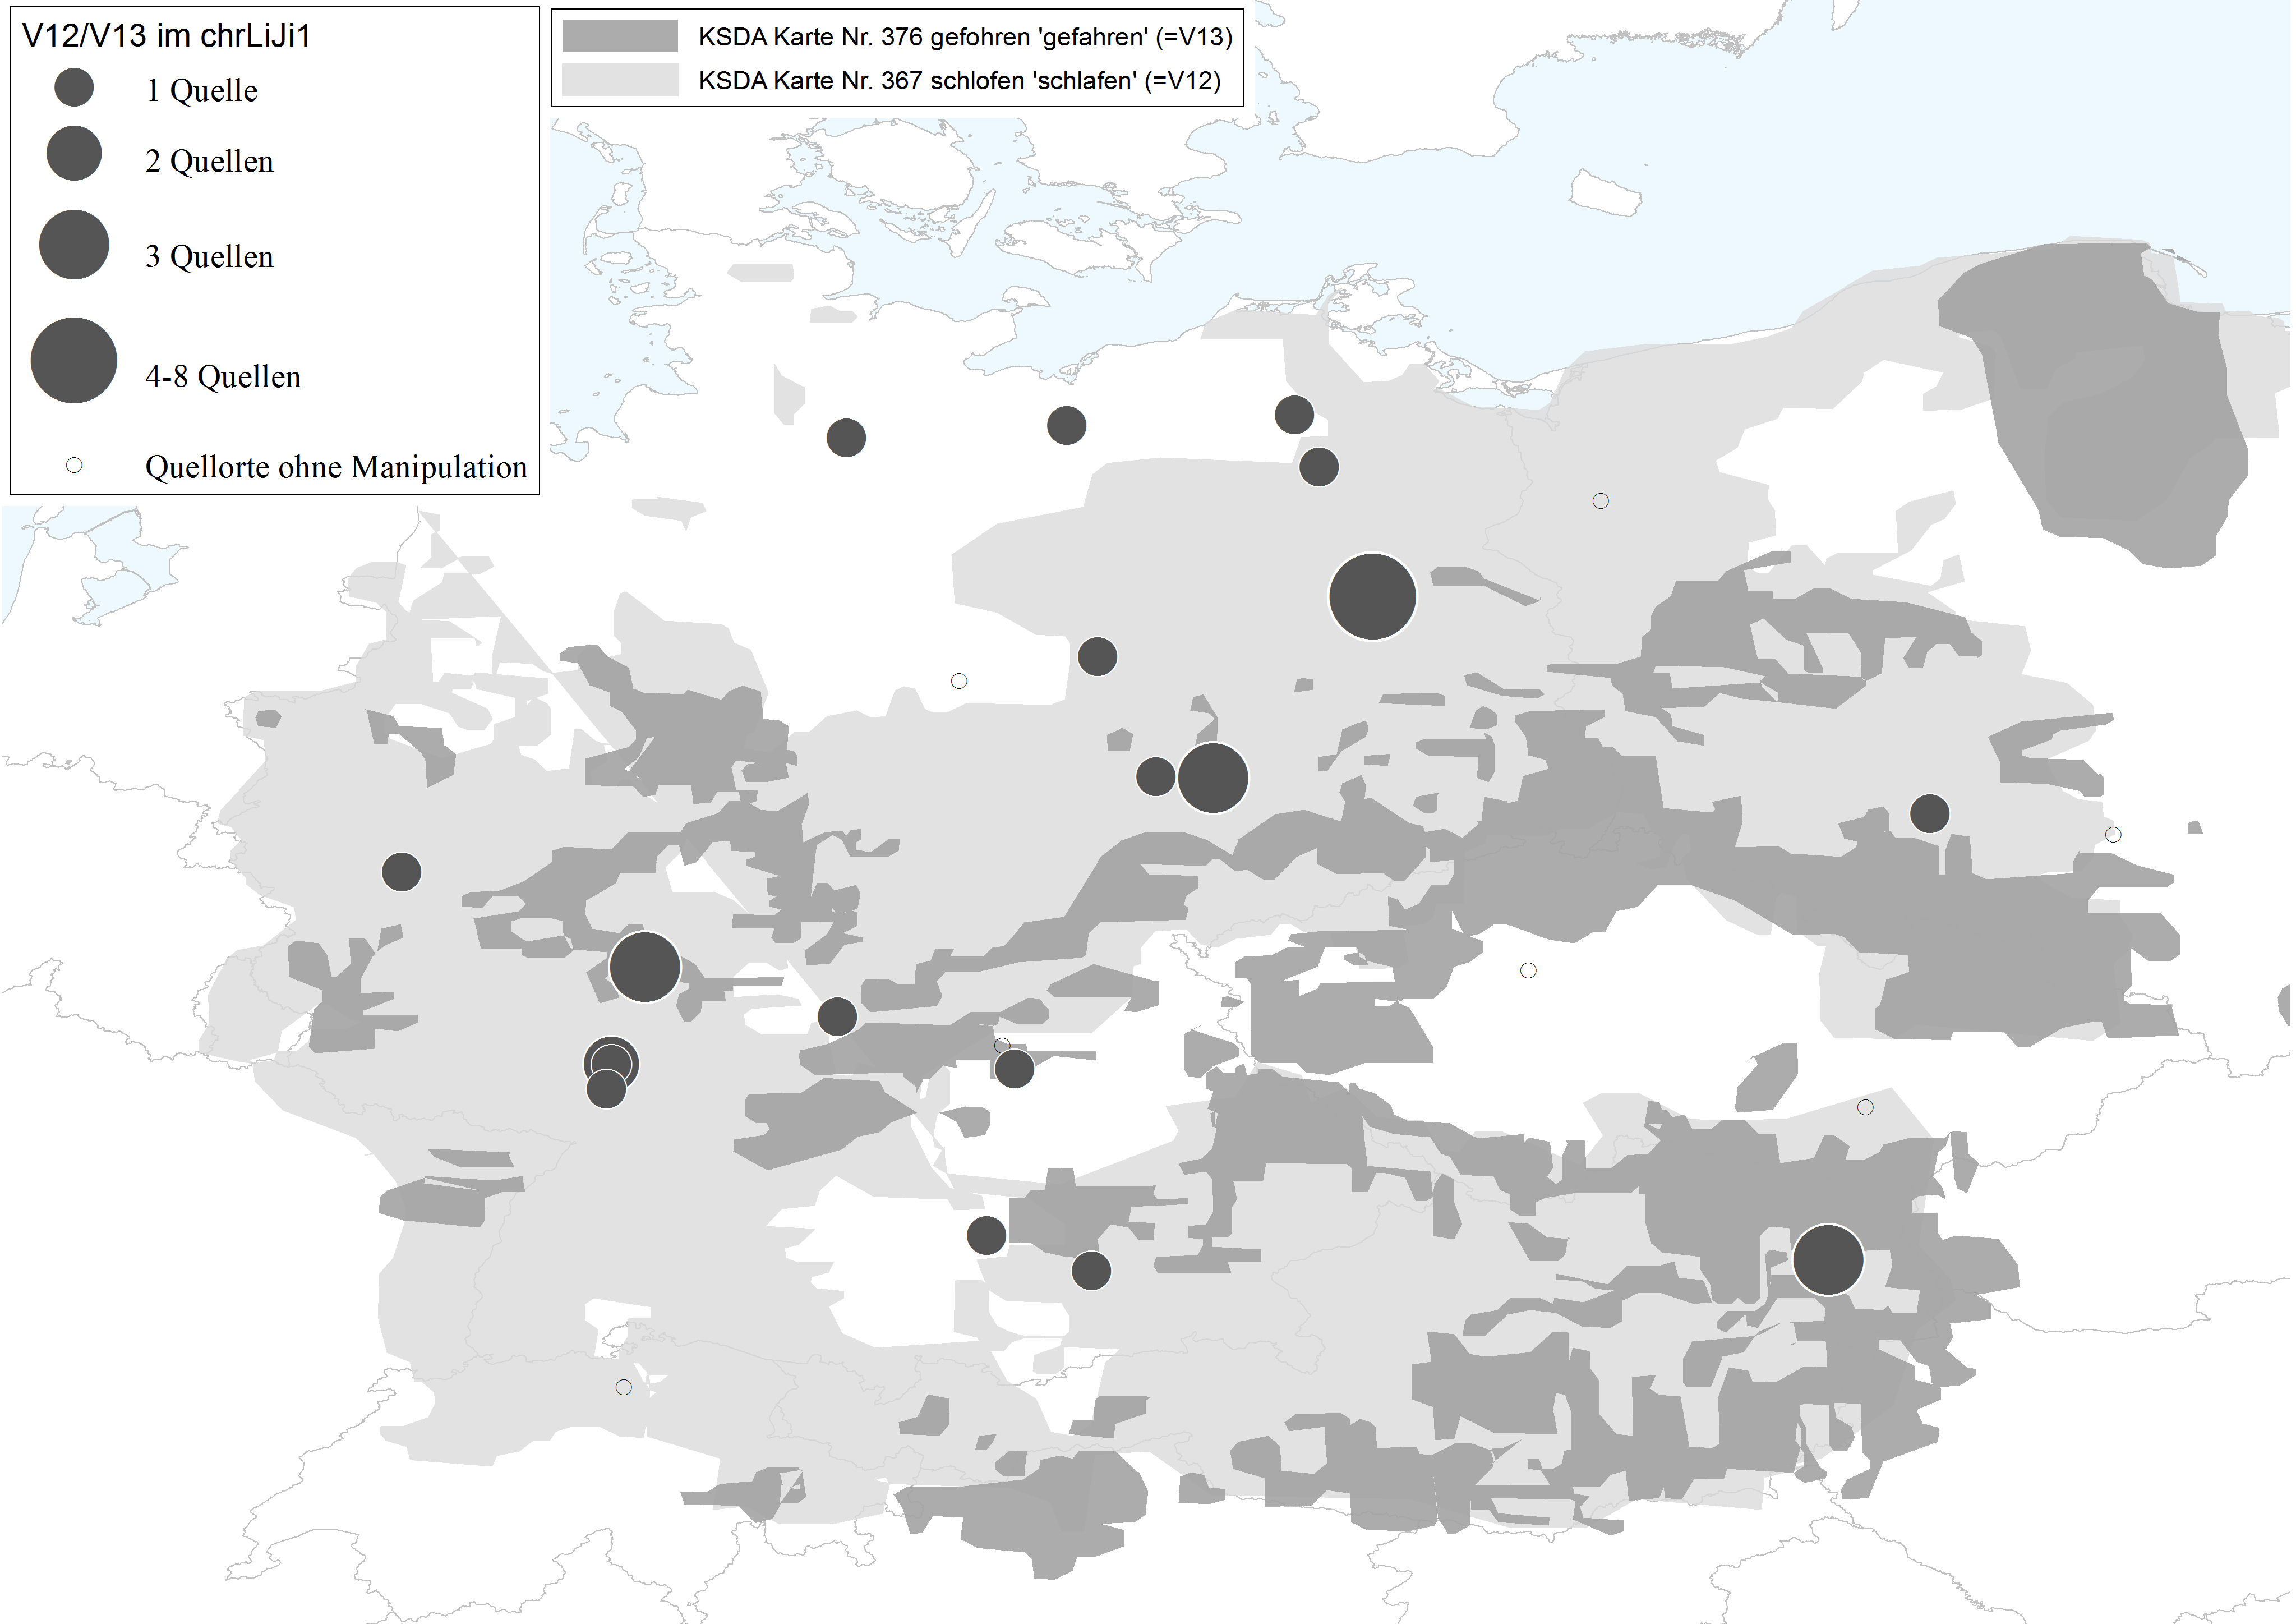
\includegraphics[width=\textwidth]{figures/karteV1213_2.png}
		\caption{\label{karteV1213}  \hai{V12}/\hai{V13} im \hai{chrLiJi1} mit \hai{KDSA} Karten Nr. 376, 367}
		\end{figure}


  
  
  
 Auch im \hai{jüdLiJi1} finden sich die Verdumpfung von \hai{V12} und \hai{V13}. Alle Texte, bis auf einen,\footnote{Dabei handelt es sich um die Quelle \hai{PBerlin1}.}  zeigen <o> an der Position von \hai{V12}. In zwei Quellen ist jedoch die Verdumpfung von \hai{V11} am Lexem \sem{fragen} belegt (\hai{GuS23}:\,5, 6;\, \hai{PAlsleben}:\,3) und damit an demselben Lexem, welches auch im \hai{chrLiJi1}  in dieser Form auftritt (s.\,o.). 
 
 
 Da die Verdumpfung ein für Muttersprachler des Deutschen recht zugängliches Phänomen ist, überrascht es, dass Hyperkorrekturen, also die Verdumpfung von \hai{V11}, wie etwa \textit{Sproche} \sem{Sprache} oder \textit{Gost} \sem{Gast}, nicht häufiger auftreten. Dass dies nicht der Fall ist, spricht m.\,E. ganz besonders für die Akkuratheit der Imitationen, egal in welchem Stadium des \hai{{\LiJi}}. Die Verdumpfung von \hai{V11} hat in den deutschen Dialekten zwar seltener stattgefunden, als diejenige von \hai{V12} und \hai{V13}, ist aber besonders in mitteldeutschen und bairischen Varietäten gegeben (vgl.\, \hai{WA} Karte Nr. 360  \sem{Nacht} u. \hai{WEK} \sem{diese Nacht}). Ein Einfluss der Matrixsprache der Autoren auf die Verdumpfung ist demnach weitestgehend auszuschließen. Eine zwischen \hai{V12} und \hai{V13} (und \hai{V42}) näher differenzierende Analyse bedarf jedoch Grundlagenarbeit zum mittelhochdeutschen, protojiddischen und westjiddischen Vokalsystem.
  
   
  
 \section{\textit{o} > \textit{u} und \textit{u} > \textit{o}}\label{o_u_zeug}

Die zwei komplementären Entwicklungen der Hebung von \textit{o} und der Senkung von \textit{u} sind ein bekanntes Phänomen der ostjiddischen Dialekte. Für das \hai{{\WJ}} fehlen allerdings noch immer flächendeckende Untersuchungen. Mit Hilfe des \hai{{\LiJi}} wollen die folgenden Unterabschnitte zeigen, dass Hebung und Senkung nicht auf das ostjiddische Dialektgebiet beschränkte Ereignisse sind.


 \subsection{Hebung von /\textit{o}/ > /\textit{u}/ (vor Nasal)}\label{o_u} 

 Ein Charakteristikum des \hai{{\ZOJ}} und \hai{{\SOJ}} ist die Hebung von \hai{V12} und die Verdumpfung von \hai{V13} > /\textit{u}/ (\citealt[66]{Herzog1992};\citealt[28]{Beider2010}). Die Karte des \hai{LCAAJ} (\citeyear[66–68]{Herzog1992}), zeigt, dass dieses Phänomen auch vereinzelt Hebraismen das \hai{{\WJ}} betroffen hat. Eine Detailanalyse zur Situation im \hai{{\WJ}} steht jedoch noch aus. Immerhin zeigt eine der authentischsten Quellen des \hai{ZWJ}, \qu{Die Hochzeit zu Grobsdorf} (1822), diese Hebung von /\textit{o}/ > /\textit{u}/ mehrfach, wie z.\,B.\, am Verb \sem{kommen} (\ref{bspgrob1}) oder den Präpositionen \sem{von} (\ref{bspgrob2}) und \sem{wo} (\ref{bspgrob3}). Diese Hebung hat in den koterritorialen zentralhessischen Dialekten nicht stattgefunden, sondern \,%rs Komma fehlt
 überwiegend die ostmitteldeutschen, rheinfränkischen und \,%rs "und" ergänzen
 alemannischen Dialekte sowie das Südbairische des Burgenlands betroffen (vgl.\, Karte \ref{karteou};\hai{SDS} Karte Nr. I/46;\, \hai{WEK} \sem{solche}). Dementsprechend korrekt ist sie auch nicht in den Passagen aus \qu{\RL{דיע ה{א\makebox(-1.25,-1.25)[r]{\libertineGlyph{uni05B8}}}כצייט צו גר{א\makebox(-1.25,-1.25)[r]{\libertineGlyph{uni05B8}}}בסד{א\makebox(-1.25,-1.25)[r]{\libertineGlyph{uni05B8}}}רף}} (\sem{Die Hochzeit zu Grobsdorf}) umgesetzt, in denen nicht-jüdische Bevölkerung spricht (\ref{bspgrob4}). Als eine weitere Quelle, die diese Hebung zeigt, sei Wolfssohns maskilisches Stück \qu{\RL{לייכטזין אונד {פ\makebox(-0.8,9)[r]{\libertineGlyph{uni207B}}}רעממעלייא}}  (\sem{Leichtsinn und Frömmelei}) angeführt (\ref{bspleicht2}). So darf angenommen werden, dass die Hebung von /\textit{o}/ > /\textit{u}/ teilweise auch im \hai{{\WJ}} stattgefunden hat.

 \eenumsentence{
	\item \RL{ עס קוממע נ{א\makebox(-1.25,-1.25)[r]{\libertineGlyph{uni05B8}}}ך גא\makebox(-1.5,-7.5)[r]{\libertineGlyph{uni207B}}ר {פ\makebox(-0.8,9)[r]{\libertineGlyph{uni207B}}}יעל לייט.
 } \\
\textit{es kumme nokh gar fiel leyt}\\
\sem{Es kommen noch gar viele Leute} 
	\\ (\qu{Die Hochzeit zu Grobsdorf} 1822:\,15)
\label{bspgrob1} 

	\item \RL{ ד{א\makebox(-1.25,-1.25)[r]{\libertineGlyph{uni05B8}}}ס דוא פון גר{א\makebox(-1.25,-1.25)[r]{\libertineGlyph{uni05B8}}}בסדארף ביסט.
 }
	\\
	\textit{dos du fun grobsdorf bist}\\
	\sem{dass du von/aus Grobsdorf bist}
	 \\ (\qu{Die Hochzeit zu Grobsdorf} 1822:\,9)
\label{bspgrob2} 

\item \RL{ וואו ה{א\makebox(-1.25,-1.25)[r]{\libertineGlyph{uni05B8}}}ט מער זונסט געוויסט {פ\makebox(-0.8,9)[r]{\libertineGlyph{uni207B}}}ון {פ\makebox(-0.8,9)[r]{\libertineGlyph{uni207B}}}ערליעבע!
 }
	\\
	\textit{vu hot mer zunst gevist fun ferliebe!}\\
	\sem{wo hat man sonst vom Verlieben gehört!}
	 \\ (\qu{Die Hochzeit zu Grobsdorf} 1822:\,14)
\label{bspgrob3} 


\item \RL{\RL{{ד}\makebox(-0.8,-2.1)[r]{\libertineGlyph{uni05B5}}}יע ז{א\makebox(-1.25,-1.25)[r]{\libertineGlyph{uni05B8}}} אים לעבע {פ\makebox(-0.8,9)[r]{\libertineGlyph{uni207B}}}ירק{א\makebox(-1.25,-1.25)[r]{\libertineGlyph{uni05B8}}}ממע
 }
	\\
	\textit{deie so im lebe firkomme}\\
	\sem{die so im Leben vorkommen}
	 \\ (\qu{Die Hochzeit zu Grobsdorf} 1822:\,5)
\label{bspgrob4} 


\item \RL{נ{א\makebox(-1.25,-1.25)[r]{\libertineGlyph{uni05B8}}}רר ער מעכט גערן ען אויסרייד ה{א\makebox(-1.25,-1.25)[r]{\libertineGlyph{uni05B8}}}בן אין דער קיך צו קוממען
 } \\
\textit{nor er mekht gern en ousreyd/ausreyd hobn in der kikh zu kummen}\\
\sem{nur möchte er eine Ausrede haben, um in die Küche zu kommen}
	\\ (\qu{Leichtsinn und Frömmelei} 1795/96:\,49)
\label{bspleicht2} 

          }
    
 %\todo{Nochmal im Kompilat prüfen! Zwei Punkte unter erstem Buchstaben im Bsp. "die so im Leben vorkommen" weiter nach links; kann leider nicht kompilieren :( }   
    
 Für eine Existenz der Hebung im \hai{{\WJ}} sprechen auch die Daten des \hai{jüdLiJi1}: Sieben der zehn Quellen weisen diese auf.\footnote{\label{FNo_u}Dabei handelt es sich um die Quellen \hai{GuS1}, \hai{GuS5}, \hai{GuS10}, \hai{GuS23}, \hai{PAlsleben}, \hai{PBerlin1} u. \hai{PBreslau}.} Natürlich stehen diese Quellen schon allein aufgrund ihrer geographischen Verortung im Osten des westjiddischen Sprachgebietes unter Verdacht, ostjiddische Formen zu transportieren, doch ob dies der Fall ist, kann erst die abschließende Zusammenschau aller Phänomene entscheiden.
             
Von den Quellen des \hai{chrLiJi1} zeigen 17 Texte eine Hebung von /\textit{o}/ > /\textit{u}/. Wie das Histogramm in Abbildung \ref{histoo_u} zeigt, taucht sie
vor allem im Zeitraum zwischen 1770 und 1870 auf, kommt aber auch noch in den Quellen der Jahrhundertwende zum 20. Jahrhundert vor.  

\begin{figure}
\fittable{	
	\begin{tikzpicture}
		\begin{axis}[only marks, width=0.82\textwidth,height=0.2\textheight,
		legend style={at={(1,1)},xshift=+0.2cm, yshift=-0.6cm,anchor=north west,nodes=left},
			%title={Funktionstypen des sp\"aten Westjiddisch},
			xtick={1700, 1725, 1750, 1775, 1800, 1825, 1850, 1875, 1900, 1925, 1950, 1975}, ytick=\empty,
			x tick label style={/pgf/number format/1000 sep=}, 
			y tick label style={/pgf/number format/1000 sep=},
			%extra y ticks={456.1, 1022.4},
			%extra y tick labels={{456,1},{1022,4}},
			extra y tick style={grid=major,
				tick label style={, ,}},
				ymin=0.7,
				ymax=2.9,
			ylabel={Phänomenbelege},
			enlarge x limits=0.03]	
	
			
\addplot [mark=*, black] table [x=jahr, y=phaen] {figures/o_u.txt};%2

\addplot [mark=o, black] table [x=jahr, y=no] {figures/o_u_no.txt};%1.5

						\legend{Hebung /\textit{o}/ > /\textit{u}/, unmanipuliert} %macht Legende
		\end{axis}
	\end{tikzpicture}
}
	\caption{Die Hebung von /\textit{o}/ > /\textit{u}/ im \hai{chrLiJi1}}
	\label{histoo_u}	
\end{figure}


Dieses Phänomen scheint besonders lexemgebunden zu sein. So findet man es im \hai{chrLiJi1} überwiegend am \isi{Infinitiv} von \sem{kommen}, an den \,%rs an den
Präpositionen \sem{von} und \sem{wo} vgl.\, (\ref{bspgrob1})--(\ref{bspgrob3}) und nur in Einzelbelegen an anderen Lexemen, z.\,B.\, \textit{Wuchen} \sem{Wochen} (\hai{AK} Zürich, 1948:\,219, 236), \textit{Sunn} \sem{Sonne} (\hai{DW} Wien, 1773:\,66;\, \hai{MV} Berlin, 1862:\,152R), \textit{Trummler} \sem{Trommler} (\hai{FS} Schwerin, 1805:\,73). 

Im \hai{chrLiJi1} tritt die Hebung \,%rs ändern zu "die Hebung"
überwiegend an Quellorten in Erscheinung, an denen sie im deutschen Dialekt ebenfalls stattgefunden hat. Es kann demnach nicht entschieden werden, ob hier eine tatsächlich westjiddische Form wiedergegeben wird oder die des örtlichen deutschen Dialekts. Lediglich drei Quellorte (Berlin, Stavenhagen, Zürich) weisen die Hebung auf. Doch gerade in den Großstädten und in polnischer\il{polnisch} Grenznähe kann ein Einfluss des \hai{{\OJ}} nicht vollständig ausgeschlossen werden.

 \begin{figure}
		\centering
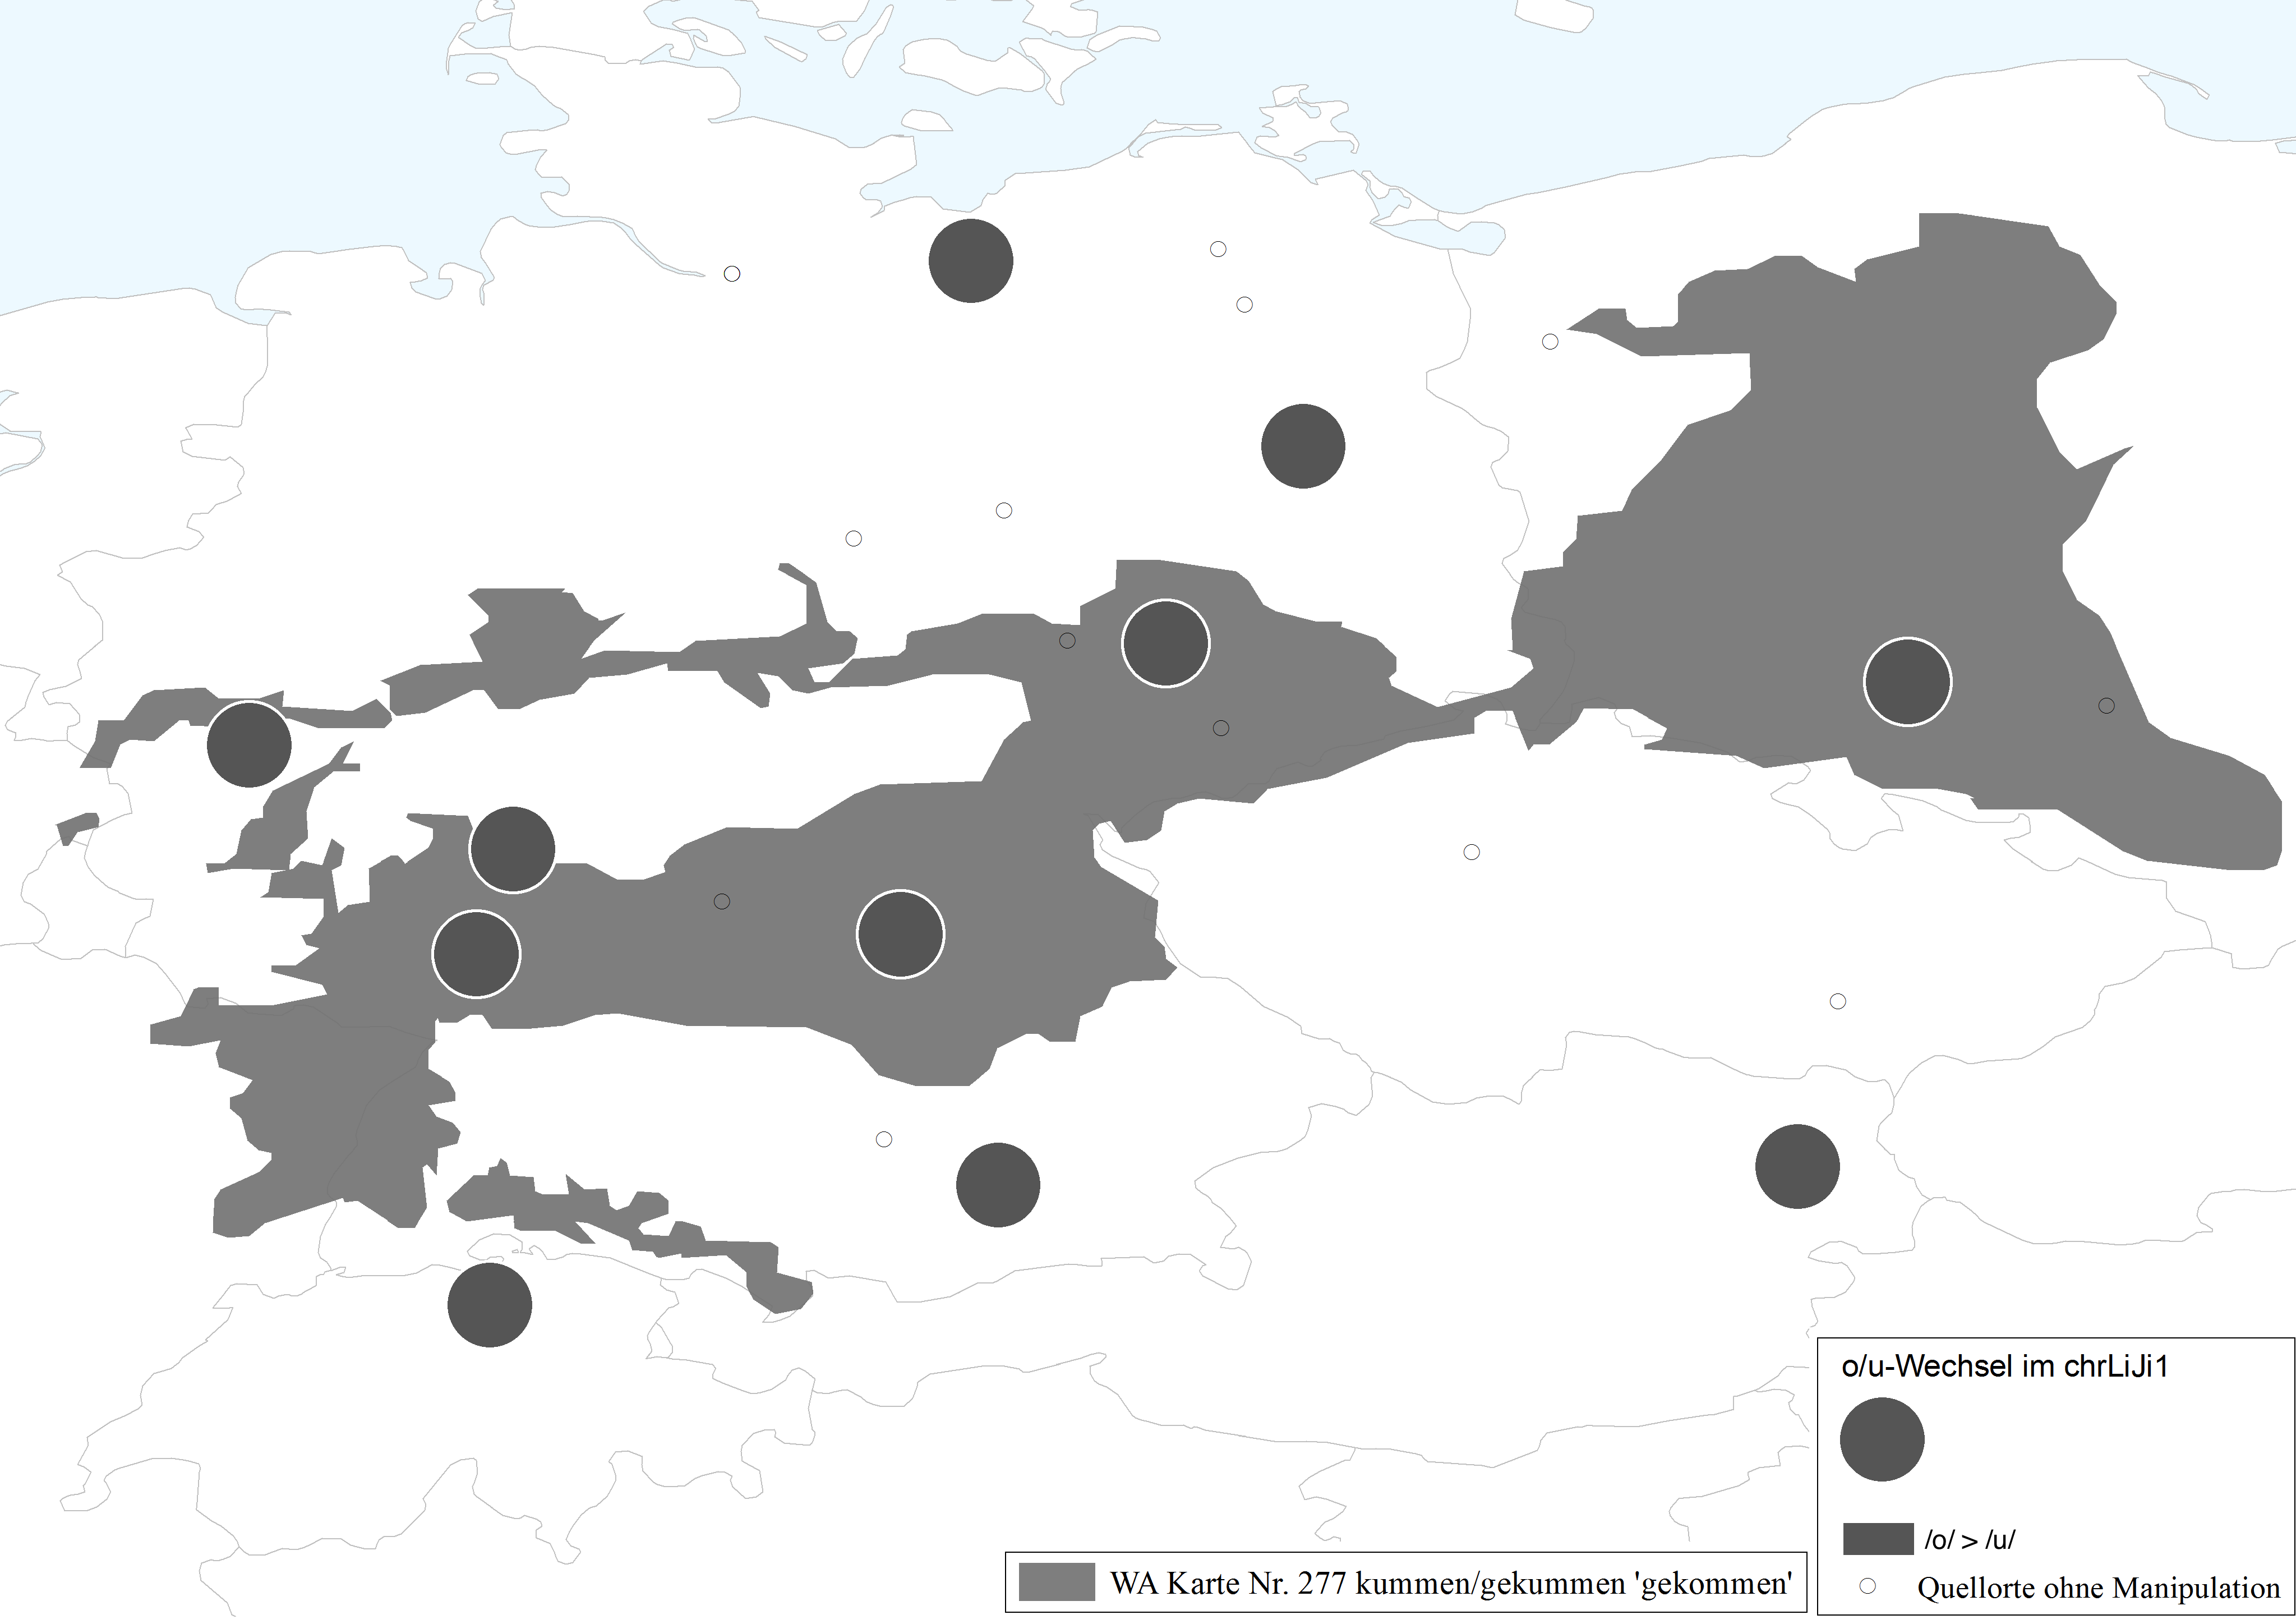
\includegraphics[width=\textwidth]{figures/karteou2.png}
		\caption{\label{karteou} o > u im \hai{chrLiJi1} mit \hai{WA} Karte Nr. 277}
		\end{figure}

		
		

 \subsection{Senkung von /\textit{u}/ > /\textit{o}/} \label{u_o} 
 %  %\noindent
Im \hai{{\ZOJ}} und westlichen Teil des \hai{{\SOJ}} hat eine Senkung von \hai{V51} (vor Liquid)  > /\textit{o}/ stattgefunden (\citealt[84]{Herzog1992}). 
Zum \hai{{\WJ}} liegen dem \hai{LCAAJ} \qu{no information} vor (\citealt[84]{Herzog1992}). Wieder kann \qu{Die Hochzeit zu Grobsdorf} helfen, das Bild vom \hai{{\WJ}} zu erweitern. Wie (\ref{bspgrob5})–(\ref{bspgrob6}) zeigen, finden wir dort parallel zur Hebung von /\textit{o}/ > /\textit{u}/ die Senkung von /\textit{u}/ > /\textit{o}/. Im \hai{ZWJ} des als \quein{Fürther Megille} bekannten Stücks \qu{\RL{אסתר. {א\makebox(-1.25,-1.25)[r]{\libertineGlyph{uni05B8}}}דער דיע בעל{א\makebox(-1.25,-1.25)[r]{\libertineGlyph{uni05B8}}}הנטע טוגענד}} %format!  Diakritikum prüfen
(\sem{Esther. Oder die belohnte Tugend};\ref{bspesther1}) wie auch im geographisch zwischen \hai{ZWJ} und \hai{{\SÜJ}} schwer verortbarem 
Stück \qu{\RL{לייכטזין אונד {פ\makebox(-0.8,9)[r]{\libertineGlyph{uni207B}}}רעממעלייא}} \sem{Leichtsinn und Frömmelei} (\ref{bspleicht1};vgl.\, \citealt[421]{FleischerSchaefer2012}) lässt sich diese Senkung finden. Allem Anschein nach sind die hier behandelte Hebung und Senkung jedoch vorrangig  Phänomene des \hai{ZWJ}, jedenfalls konnten keine Belege aus anderen Dialektregionen gefunden werden. Eine Einzelanalyse zur Situation im \hai{{\WJ}} steht allerdings noch aus, um dies mit Gewissheit sagen zu können.


 \eenumsentence{
	\item \RL{ דוא ז{א\makebox(-1.25,-1.25)[r]{\libertineGlyph{uni05B8}}}ללסט ניקס צו ק{א\makebox(-1.25,-1.25)[r]{\libertineGlyph{uni05B8}}}רץ קוממע
 } \\
\textit{du zollst niks zu korts kumme}\\
\sem{Du sollst nicht zu kurz kommen} 
	\\ (\qu{Die Hochzeit zu Grobsdorf} 1822:\,108)
\label{bspgrob5} 


\item \RL{ד{א\makebox(-1.25,-1.25)[r]{\libertineGlyph{uni05B8}}}רך שא\makebox(-1.5,-7.5)[r]{\libertineGlyph{uni207B}}רע ווערד מער קלוג
 } \\
\textit{dorkh share verd mer klug}\\
\sem{Durch Schaden wird man klug} 
	\\ (\qu{Die Hochzeit zu Grobsdorf} 1822:\,12)
\label{bspgrob6} 




\item \RL{דוי גיהט נ{א\makebox(-1.25,-1.25)[r]{\libertineGlyph{uni05B8}}}ר ניט ריין אין דער שטוב
 } \\
\textit{dou/dau giht nor nit reyn in der shtub}\\
\sem{da geht nur nicht herein in die Stube}
	\\ (\qu{Esther. Oder die belohnte Tugend} 1828:\,56)
\label{bspesther1} 


\item \RL{נ{א\makebox(-1.25,-1.25)[r]{\libertineGlyph{uni05B8}}}רר ער מעכט גערן ען אויסרייד ה{א\makebox(-1.25,-1.25)[r]{\libertineGlyph{uni05B8}}}בן אין דער קיך צו קוממען
 } \\
\textit{nor er mekht gern en ousreyd/ausreyd hobn in der kikh zu kummen}\\
\sem{nur möchte er eine Ausrede haben, um in die Küche zu kommen}
	\\ (\qu{Leichtsinn und Frömmelei} 1795/96:\,49)
\label{bspleicht1} 


}

Diese Senkung fand 
% allerdings 
jedoch %\todo{allerdings $\to$ jedoch}
auch in den koterritorialen süd-zentral\-hes\-sichen Mundarten statt und könnte daher in \qu{Der Hochzeit zu Grobsdorf} ein Interferenzereignis darstellen. Allgemein ist die Senkung in den deutschen Dialekten von /\textit{u}/ > /\textit{o}/ weitaus weniger verbreitet als die Hebung zu /\textit{u}/ (Karten in Abbildung \ref{karteuo} u. \ref{karteouuoall}). Die Senkung fand neben dem Zentralhessischen vor allem im Rhein- und Moselfränkischen, in Teilen des Obersächsischen und Ostfälischen, im Westen der deutschsprachigen Schweiz (\hai{SDS} Karte Nr. I/51) sowie verstreut im Schlesischen und anderen Siedlungsmundarten statt. 

Die 14 Quellen des \hai{chrLiJi1}, welche die Senkung zeigen, finden sich überwiegend in der ersten Hälfte des 19. Jahrhunderts, später tritt die Senkung aber immernoch regelmäßig auf (Abbildung \ref{histou_o}).


 %%%u > o Diagramm%\begin{flushleft}	
\begin{figure}
 \fittable{
	\begin{tikzpicture}
		\begin{axis}[only marks, width=0.82\textwidth,height=0.2\textheight,
		legend style={at={(1,1)},xshift=+0.2cm, yshift=-0.6cm,anchor=north west,nodes=left},
			%title={Funktionstypen des sp\"aten Westjiddisch},
			xtick={1700, 1725, 1750, 1775, 1800, 1825, 1850, 1875, 1900, 1925, 1950, 1975}, ytick=\empty,
			x tick label style={/pgf/number format/1000 sep=}, 
			y tick label style={/pgf/number format/1000 sep=},
			%extra y ticks={456.1, 1022.4},
			%extra y tick labels={{456,1},{1022,4}},
			extra y tick style={grid=major,
				tick label style={, ,}},
				ymin=0.7,
				ymax=2.9,
			ylabel={Phänomenbelege},
			enlarge x limits=0.03]	
	
			
\addplot [mark=*, black] table [x=jahr, y=phaen] {figures/u_o.txt};%2

\addplot [mark=o, black] table [x=jahr, y=no] {figures/u_o_no.txt};%1.5


 

			% Andere Formen a={mark=square*,blue},% b={mark=triangle*,red},% c={mark=o,draw=black}}
						\legend{Senkung /\textit{u}/ > /\textit{o}/, unmanipuliert} %macht Legende
		\end{axis}
	\end{tikzpicture}
}
	\caption{Die Senkung von /\textit{u}/ > /\textit{o}/ im \hai{chrLiJi1}}
	\label{histou_o}	
\end{figure}



Die Kartierung der Korpusbelege zeigt, dass die Senkung vermehrt auch in Regionen durchgeführt wurde, in denen sie in den deutschen Mundarten unüblich ist (Abbildung \ref{karteuo}). Viele Belegorte, die in einem Gebiet liegen, in welchem die Senkung im Deutschen belegt ist, zeigen allerdings keine Manipulation von /\textit{u}/ > /\textit{o}/ im \hai{chrLiJi1}, dies schwächt einen Erklärungsversuch auf Basis eines potenziellen Einflusses der deutschen Dialekte auf das \hai{chrLiJi1} zusätzlich ab.  
 
  \begin{figure}
		\centering
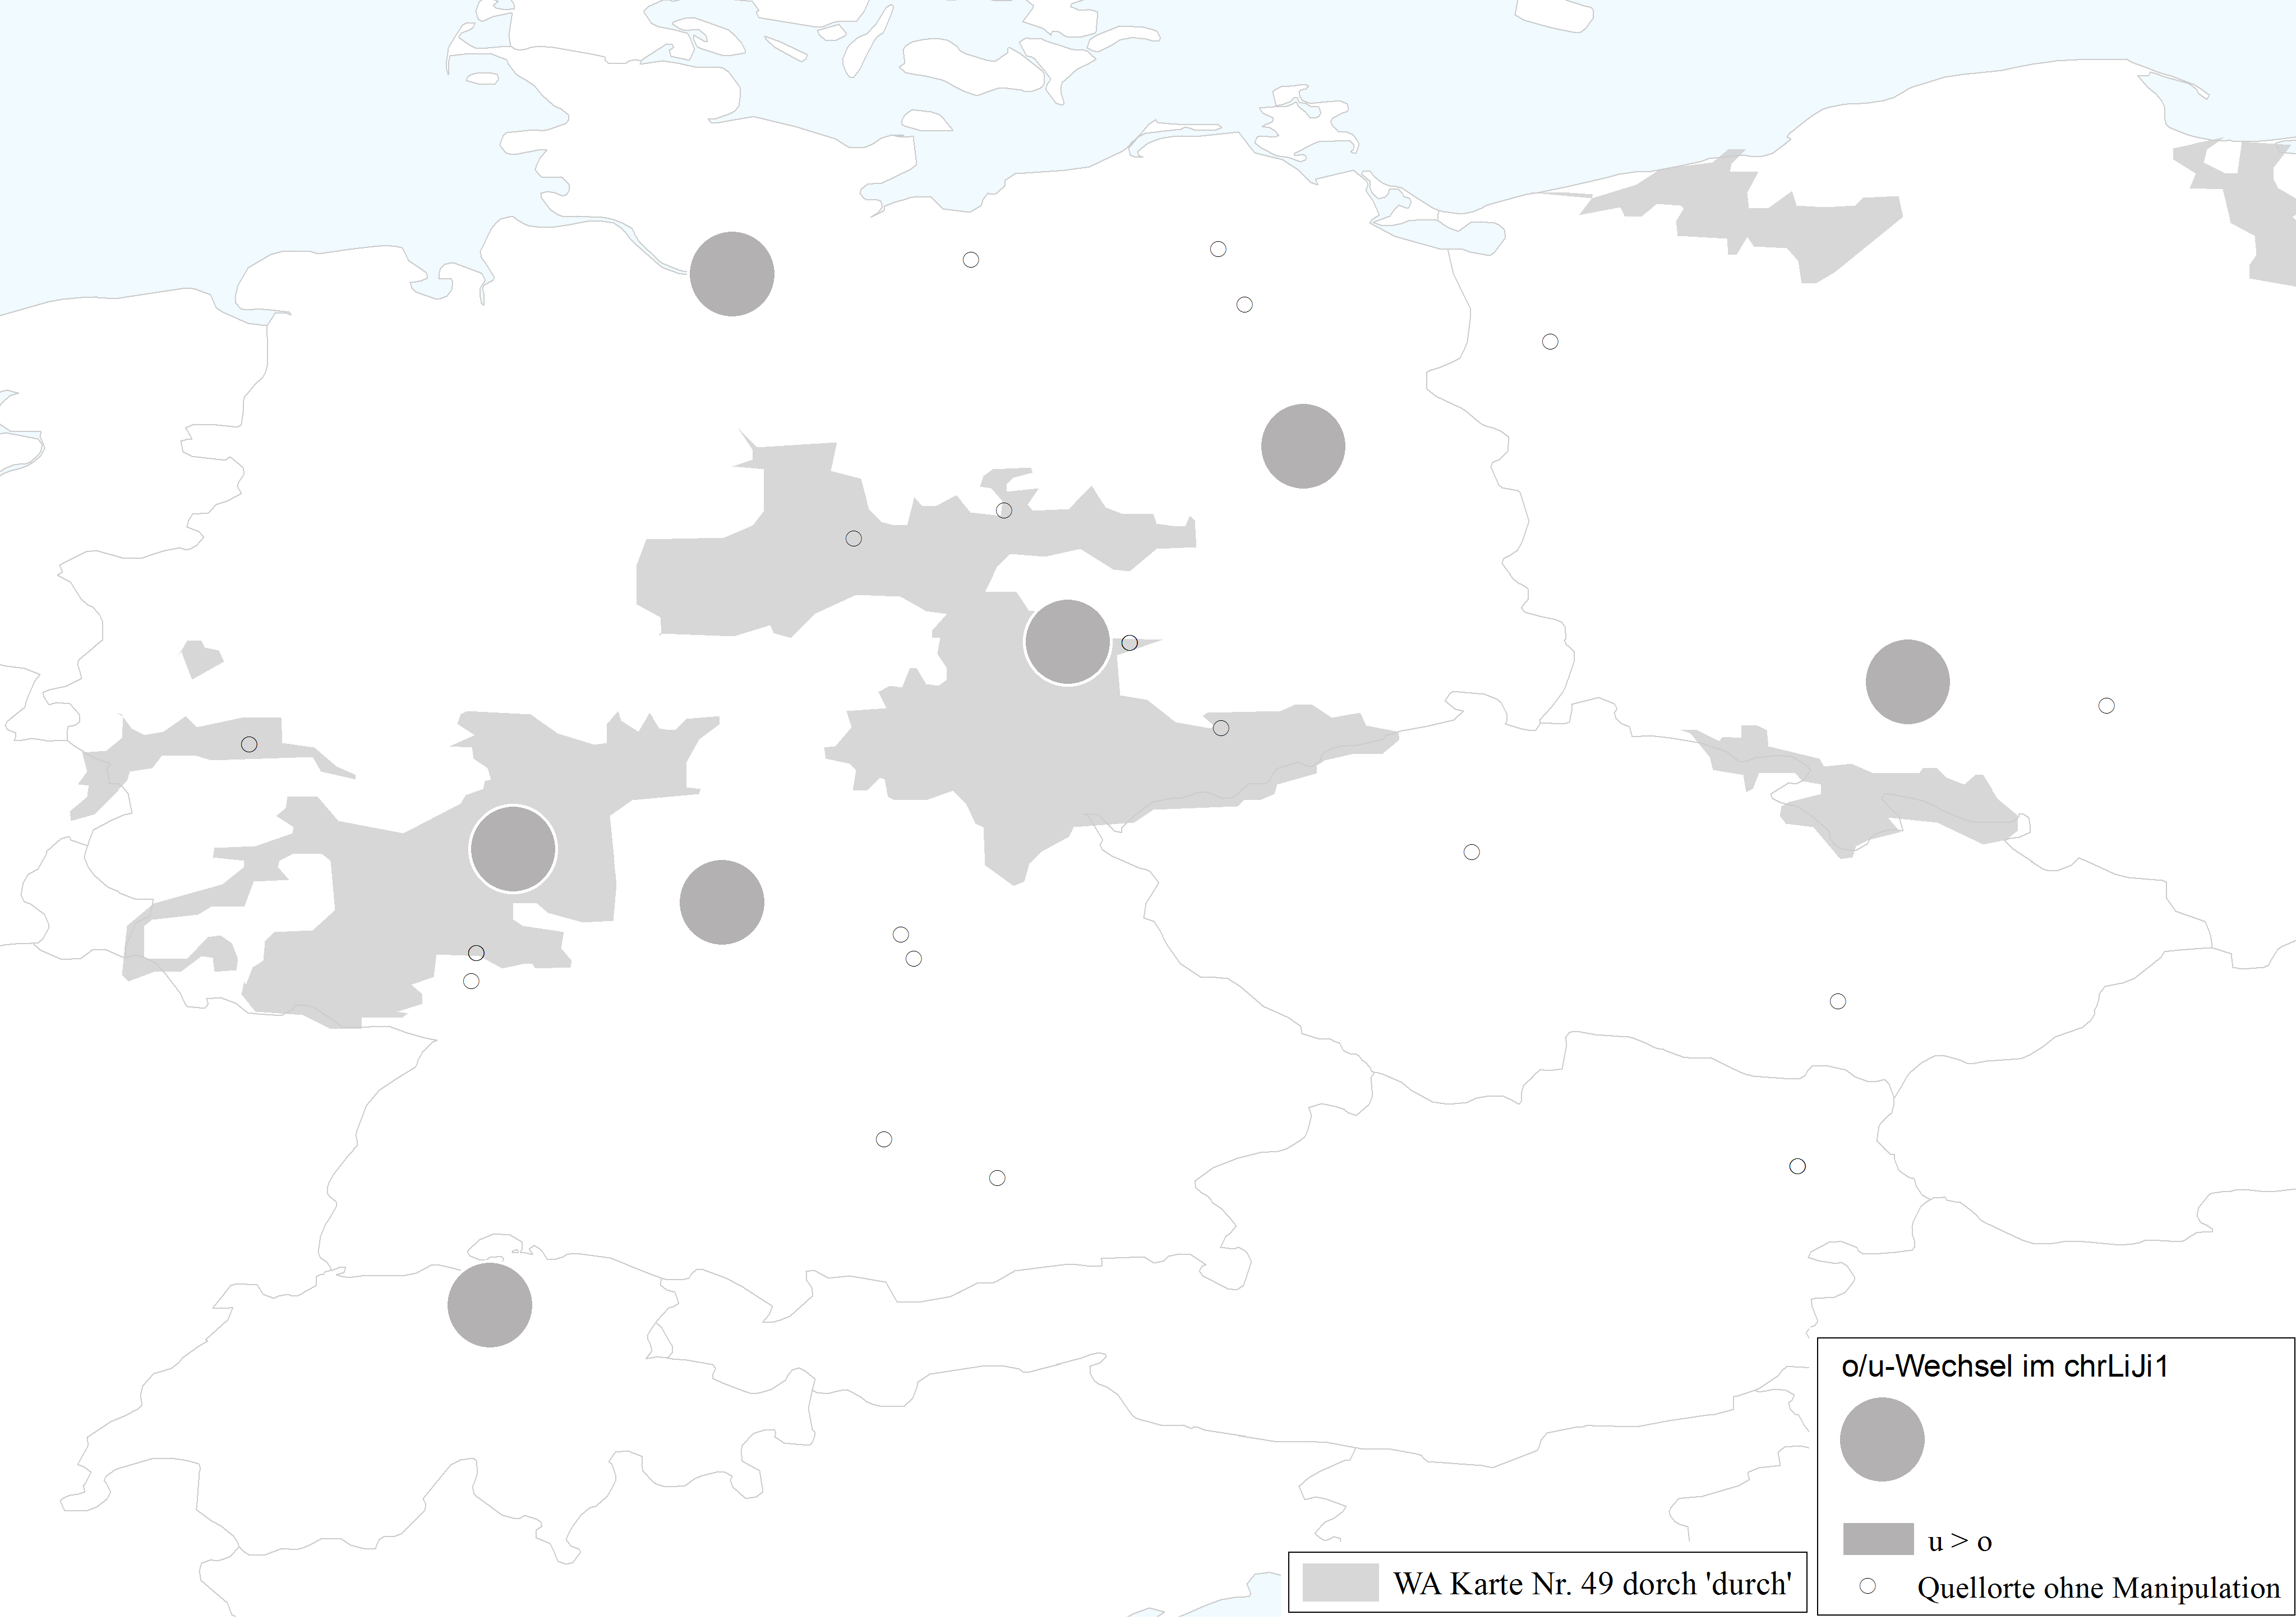
\includegraphics[width=\textwidth]{figures/karteuo.png}
		\caption{\label{karteuo} Der Wechsel von /\textit{o}/ > /\textit{u}/ im \hai{chrLiJi1} mit \hai{WA} Karte Nr. 49}
		\end{figure}



Das Phänomen der Senkung von /\textit{u}/ > /\textit{o}/ eignet sich bestens, um den diatopischen Vorteil literaturjiddischer Texte als Sekundärquellen des Westjiddischen zu illustrieren. In der Karte Nr. 35 des \hai{LCAAJ} ist die Situation im Westjiddischen (mit Ausnahme der Situation im \hai{{\SWJ}} Strasbourgs) mit \qu{? no information} versehen (vgl.\, \hai{LCAAJ} Karte Nr. 35). Die Senkung selbst ist lediglich im \hai{{\ZOJ}} und südlichen \hai{{\NÜJ}} belegt. Vereint man nun die Daten authentischer westjiddischer Quellen %(\ref{bspgrob5}–\ref{bspleicht1}) 
mit den Daten zum \hai{chrLiJi1}, so ergibt sich ein  Kontinuum der Senkung in allen westjiddischen Varietäten bis weit in das ostjiddische Gebiet hinein.\label{ProtoLCAAJOEWY2}% (vgl.\, Abbildung \ref{ProtoLCAAJOEWY2}b).
 
 % \begin{center}
  %\begin{figure}
 % \fittable{
 %\subfloat[Unbearbeiteter Scan der \hai{LCAAJ} Karte Nr. 35 \hai{U\textsubscript{1}} before \textit{r}]{\includegraphics[width=1.12\textwidth]{figures/LCAAJ_U1_blanko.png}}

 %\subfloat[Unbearbeiteter Scan der \hai{LCAAJ} Karte Nr. 35 inkl. Belege der Haskala Stücke und \hai{chrLiJi1} Daten]{\includegraphics[width=1.12\textwidth]{figures/LCAAJ_U1_Proto.png}}

 %}
 %\caption{Ergänzung der \hai{LCAAJ}-Daten zur Senkung von /\textit{u}/ > /\textit{o}/ vor <r>}
 %\label{ProtoLCAAJOEWY2}
 %\end{figure}
% \end{center}
 %\todo{nebeneinander nicht zu klein? Legende nicht lesbar}
 
 
 Parallel zur Hebung von /\textit{o}/ > /\textit{u}/ (Unterabschnitt \ref{o_u}) zeigt das \hai{jüdLiJi1} die Senkung von /\textit{u}/ > /\textit{o}/ in den gleichen Quelltexten.\footnote{Diese Quellen sind: \hai{GuS1}, \hai{GuS5}, \hai{GuS10}, \hai{GuS23}, \hai{PAlsleben}, \hai{PBerlin1} u. \hai{PBreslau} (vgl.\, Fn. \ref{FNo_u}).} 
 
 
  \subsection{Zusammenhang zwischen Hebung und Senkung} \label{ou_uo}

Der durch Hebung und Senkung hervorgerufene komplementäre Wechsel von /\textit{u}/ und /\textit{o}/ wurde im \hai{chrLiJi1} in sieben Quellen durchgeführt.\footnote{In den Quellen \hai{AK} (Zürich, 1948), \hai{GW} (n.a., ca.\, 1900), \hai{JK} (Breslau, 1810), \hai{MV} (Berlin, 1862), \hai{PA} (Frankfurt, 1834), \hai{SS} (Berlin, 1907) u. \hai{VD} (Frankfurt, 1916).} Im \hai{jüdLiJi1} wurden wie bereits erwähnt (s.\,o.) Hebung und Senkung immer nur parallel durchgeführt. 

Für die Daten des christlichen wie jüdischen \hai{{\LiJieins}} ist allerdings zu bedenken, dass an den Quellorten (Breslau, Berlin, Zürich), an denen die Entwicklungen Hebung und Senkung parallel stattgefunden haben, ein ostjiddischer Einfluss nicht auszuschließen ist (s. Karte in Abbildung \ref{karteouuoall}). Dieses Phänomen könnte also auf Interferenzen zum \hai{{\OJ}} im \hai{{\LiJi}} hinweisen. In den deutschen Dialekten fand dieses doppelte Ereignis von Hebung und Senkung nur im Obersächsischen und Moselfränkischen statt (vgl.\, Abbildung \ref{karteouuoall}). Lediglich die Quellen aus Frankfurt a. M. stünden also im Verdacht, eine dialektale Entwicklung aus den deutschen Dialekten zu transportieren. Die Karte zeigt allerdings auch, dass Quellen nur eine der beiden Entwicklungen im \hai{chrLiJi1} zeigen, wenn in den koterritorialen deutschen Mundarten beide Formen belegt sind (etwa Mannheim, Leipzig).
		
\begin{figure}
		\centering
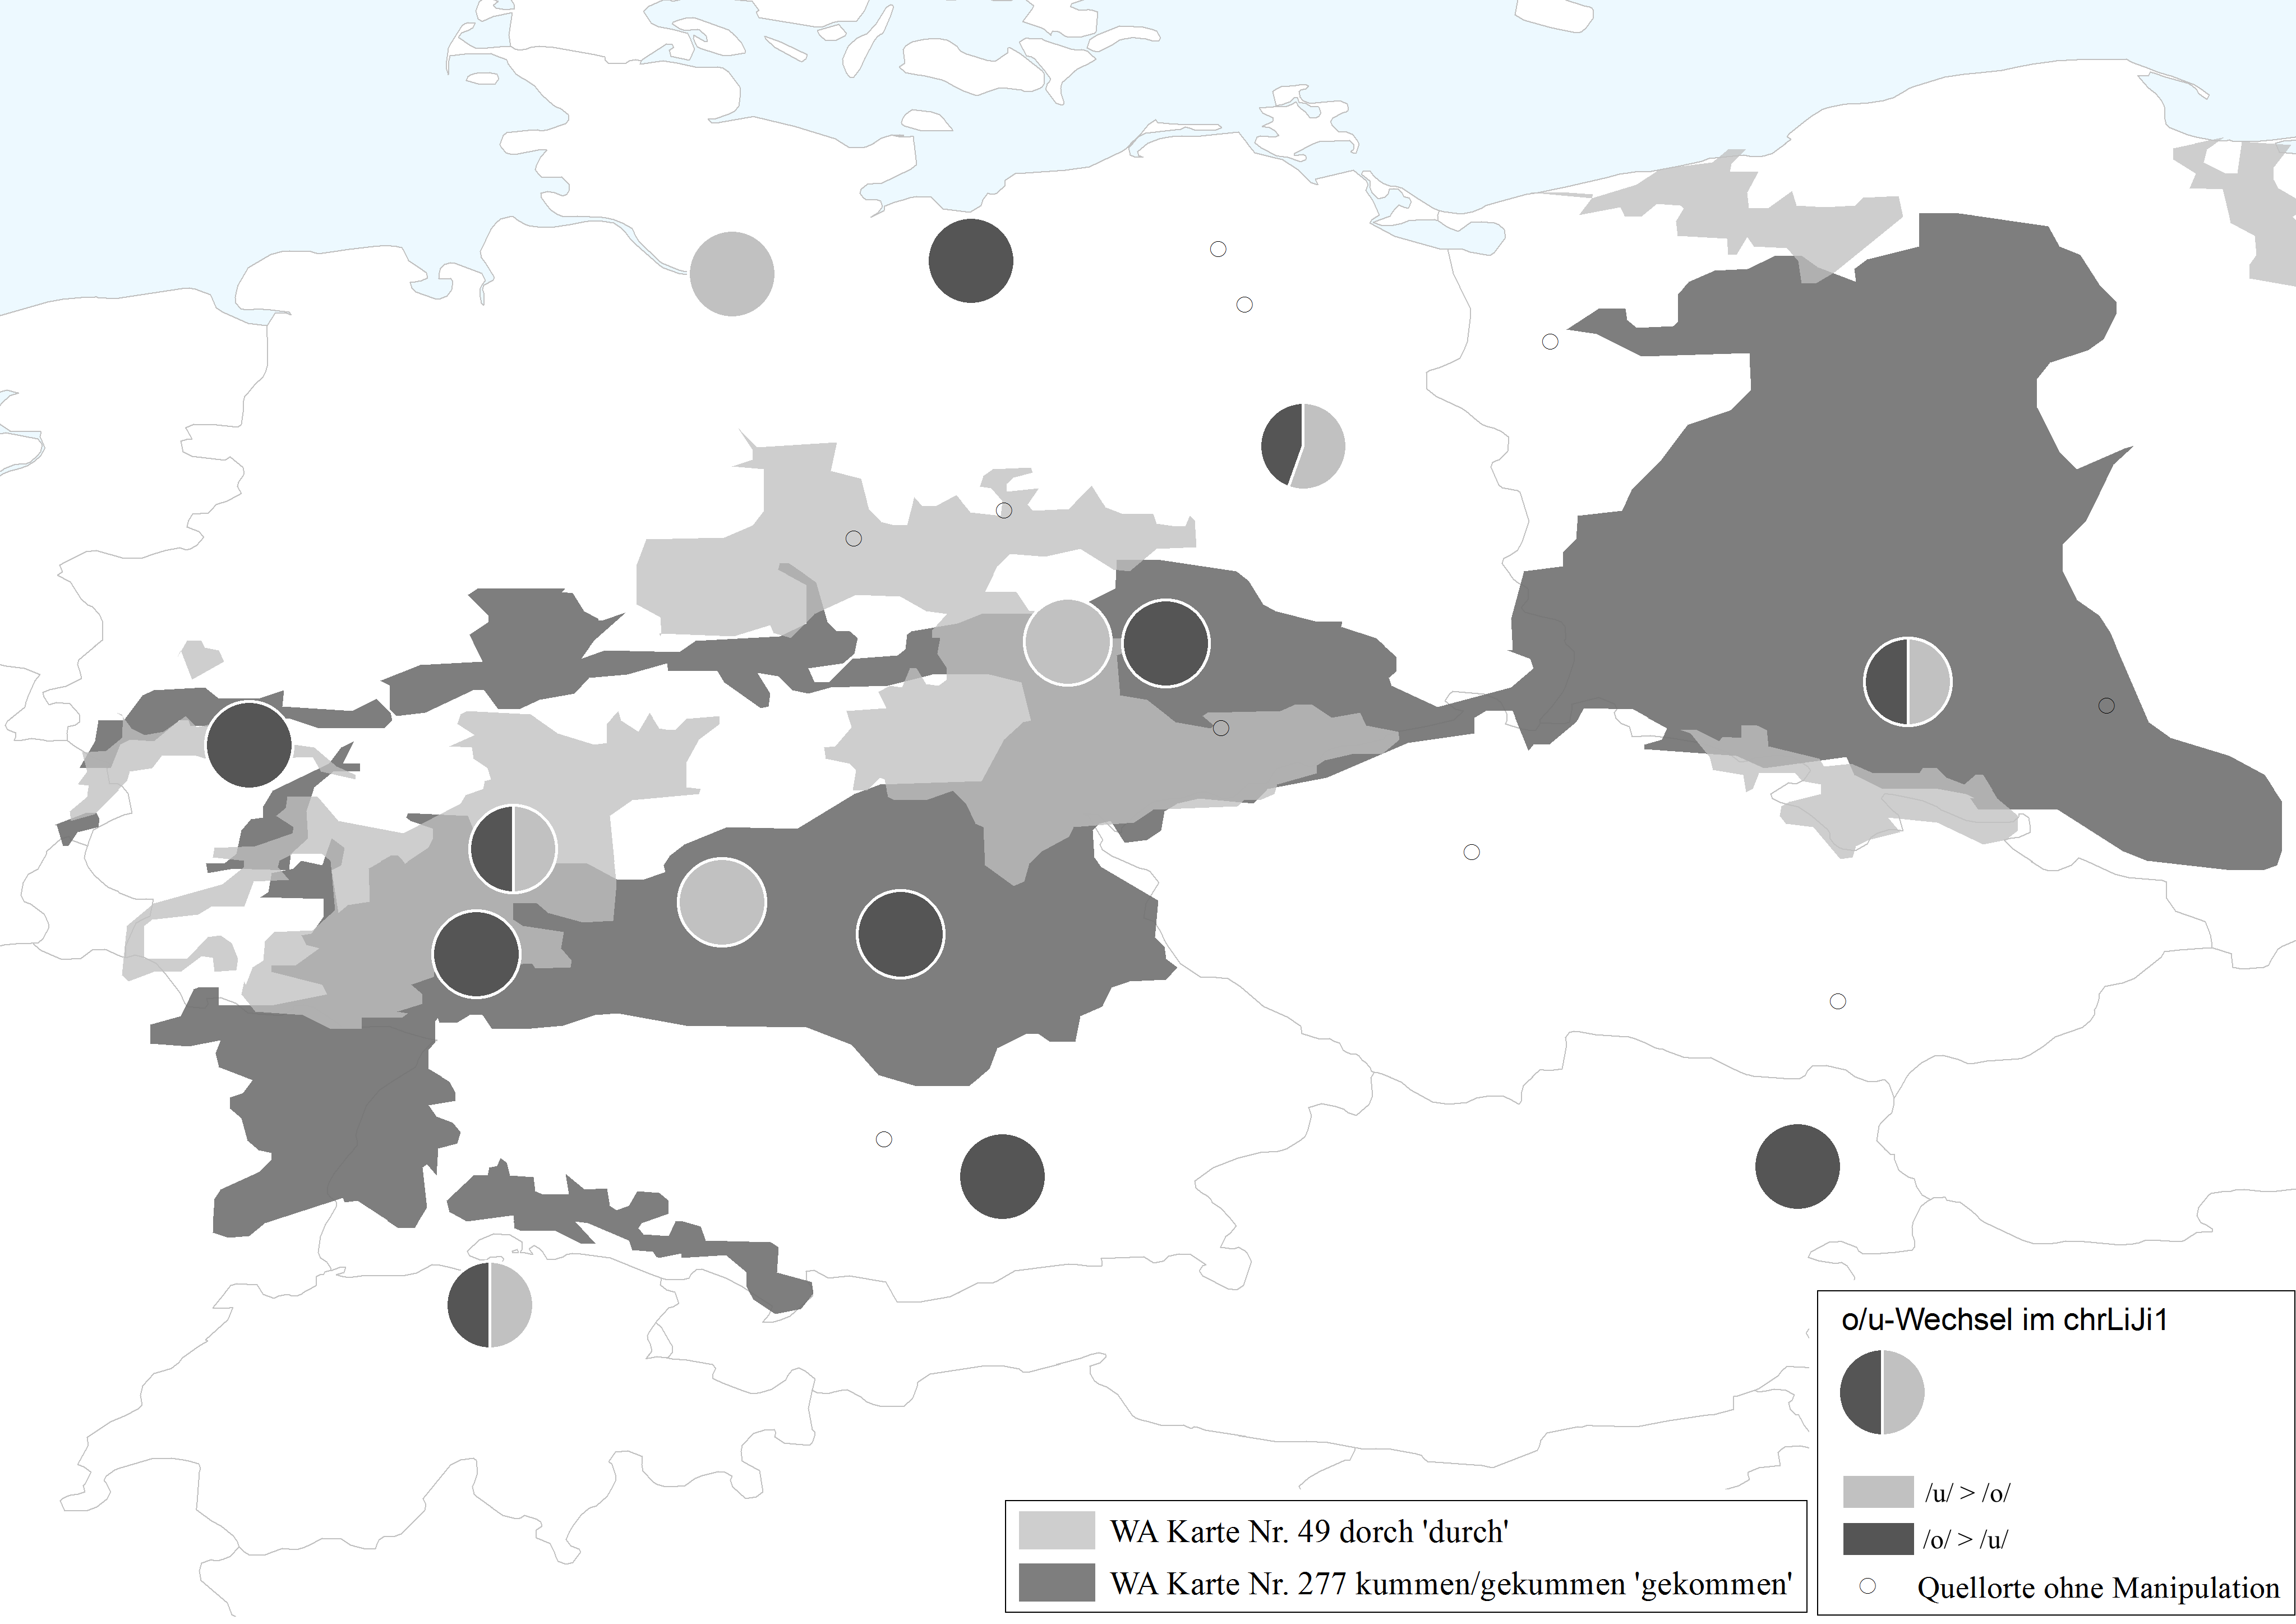
\includegraphics[width=\textwidth]{figures/karteouuoall2.png}
		\caption{\label{karteouuoall} Hebung und Senkung von /u/, /o/ im \hai{chrLiJi1} mit \hai{WA} Karten Nr. 277, 49}
		\end{figure}

		

Wie die angeführten Beispiele aus der \qu{Hochzeit zu Grobsdorf} zeigen konnten, ist jedoch nicht auszuschließen, dass dieses Phänomen nicht nur in den ostjiddischen Dialekten, sondern auch in den westjiddischen Varietäten auftritt. Der Umstand, dass in vielen Quellen nur eine Entwicklung (Hebung oder Senkung) stattgefunden hat, lässt immerhin darauf schließen, dass möglicherweise nur eine Regel des komplexen Wechsels der zwei Vokale von den Imitatoren erkannt wurde. Dies lässt an sich noch nicht ausschließen, dass das komplementäre Ereignis im \hai{{\WJ}} nicht stattgefunden hat.

 \section{Palatalisierung /u/, /u\textlengthmark/ > /y/, /y\textlengthmark/}\label{phonpalat}
 %\noindent 
 Die \isi{Palatalisierung} von /u/, /u\textlengthmark/ > /y/, /y\textlengthmark/ ist ein besonderes Merkmal des Elsässer, Burgenländer und ungarischen Jiddisch (vgl.\, \citealt{Birnbaum1934};\,\citealt[108]{GuggenheimGruenberg1973};\,\citealt[1027]{Katz1983};\,\citealt[171f]{Timm1987};\,\citealt{Hutterer1965};\,\citealt[83]{Herzog1992};\, \citealt{Schaefer2017}). Es ist anzunehmen, dass /u\textlengthmark/ > /y/ übergangsweise im Zuge der zentralostjiddischen Entwicklung von /u\textlengthmark/ zu /i/ auch im \hai{{\ZOJ}} gegeben war (\citealt{Birnbaum1934};\citealt[1029]{Katz1983}). In einem kleinen Teil des nördlichen \hai{{\SOJ}} blieb die \isi{Palatalisierung} von \hai{V51} (\hai{U\textsubscript{1}}) und \hai{V52} (\hai{U\textsubscript{2}}) erhalten (\citealt[83]{Herzog1992}). Es besteht zwischen der Elsässer-\isi{Palatalisierung}, die höchst wahrscheinlich durch den \isi{Sprachkontakt} zum Französischen begünstigt war, und der \isi{Palatalisierung} im ungarischen Raum ein wichtiger systematischer Unterschied. Während im südlichen Übergangsjiddisch Ungarns, des Burgenlandes und ggf. auch vereinzelt im \hai{{\ZOJ}} Südposens  (vgl.\, \citealt{FleischerSchaeferErsch,Schaefer2017}) Lang- und Kurzvokal (\hai{V51}, \hai{V52}, \hai{V53}) palatalisiert wurden, was zu einer Systemverschiebung geführt hat, blieb im Elsässer \ili{Westjiddisch} kurz /u/ erhalten (vgl.\, \citealt{Birnbaum1934});\, was heißt, dass hier nur der Langvokal palatalisiert wurde, (\ref{bspY1})--(\ref{bspY4}).
 
  \eenumsentence{

 \item \textit{tsü}/\textit{ts\={ü}} \sem{zu} (Budapester \hai{{\SÜJ}};\citealt[124]{Hutterer1965}) \label{bspY1}

 
 \item \textit{füks} \sem{Fuchs} (Budapester \hai{{\SÜJ}};\citealt[124]{Hutterer1965})\label{bspY2}
  
  \item \textit{zü} \sem{zu} (Elsässer \hai{{\SWJ}};\qu{Chateïsim sinn aach Laït} Mulhouse 1929:\,16)\label{bspY3}

 \item \textit{Duckser} (*\textit{Dückser}) \sem{Duckser, Feigling} \\
 (Elsässer \hai{{\SWJ}};\qu{Chateïsim sinn aach Laït} Mulhouse 1929:\,20)\label{bspY4}
  
  }


 Das Auftreten der \isi{Palatalisierung} im \hai{chrLiJi1} kann damit zum einen auf den jiddischen Dialekten des Elsässer \hai{{\SWJ}}, \hai{{\SÜJ}} und \hai{{\SOJ}} beruhen, zum anderen aber könnte die \isi{Palatalisierung} tatsächlich auch in manchen westjiddischen Dialekten stattgefunden haben oder aber die Belege stellen \quein{Fehler} dar. 
 
 In 13 Texten lassen sich Belege für die \isi{Palatalisierung} finden. Die diachrone Verteilung der Belege zeigt, dass sich diese  in den zwischen 1805 und 1825 erschienenen Quellen besonders häuft (vgl.\, Abbildung \ref{palat}). Aber bereits zwei ältere Quellen von 1770 und 1773 zeigen dieses Phänomen. In der zweiten Hälfte des 19. Jahrhunderts finden wir sie vereinzelt bis ins 20. Jahrhundert hinein.
 
  %%%palat Diagramm%\begin{flushleft}	
\begin{figure}
	\begin{tikzpicture}
		\begin{axis}[only marks, width=0.82\textwidth,height=0.2\textheight,
		legend style={at={(1,1)},xshift=+0.2cm, yshift=-0.6cm,anchor=north west,nodes=left},
			%title={Funktionstypen des sp\"aten Westjiddisch},
			xtick={1700, 1725, 1750, 1775, 1800, 1825, 1850, 1875, 1900, 1925, 1950, 1975}, ytick=\empty,
			x tick label style={/pgf/number format/1000 sep=}, 
			y tick label style={/pgf/number format/1000 sep=},
			%extra y ticks={456.1, 1022.4},
			%extra y tick labels={{456,1},{1022,4}},
			extra y tick style={grid=major,
				tick label style={, ,}},
				ymin=0.7,
				ymax=2.9,
			ylabel={Phänomenbelege},
			enlarge x limits=0.03]	
	
			
\addplot [mark=*, black] table [x=jahr, y=phaen] {figures/palat.txt};%2

\addplot [mark=o, black] table [x=jahr, y=no] {figures/palat_no.txt};%1.5

			% Andere Formen a={mark=square*,blue},% b={mark=triangle*,red},% c={mark=o,draw=black}}
						\legend{<u> als <ü>, unmanipuliert} %macht Legende
		\end{axis}
	\end{tikzpicture}
	\caption{\isi{Palatalisierung} von /\textit{u}(\textlengthmark)/ > /\textit{y}(\textlengthmark)/ im \hai{chrLiJi1}}
	\label{palat}	
\end{figure}

 
 Neun der elf Quellen zeigen die \isi{Palatalisierung} sowohl beim Lang- als auch beim Kurzvokal. Die übrigen vier Quellen haben nur an einem Lexem palatalisiert und zeigen damit auch nur bei Kurzvokal (\hai{JK} Breslau, 1810 u. \hai{TH} Merseburg, 1820) oder Langvokal (\hai{AO} Wien, 1770 u. \hai{SV} München, 1890) dieses Phänomen. Aufgrund \,%rs A
 der schmalen Datengrundlage lässt sich hier nicht feststellen, ob die Verfasser gezielt nur am Lang- bzw. Kurzvokal <ü> gesetzt haben, was prinzipiell in den Quellorten nicht anzunehmen ist. 
 
 Besonders auffällig gestalten sich die Belege zur \isi{Palatalisierung} in ihrer räumlichen Verteilung (s. Abbildung \ref{kartepalat}). Sie tritt ausschließlich in östlichen Quelltexten auf und ganz besonders in Texten aus Berlin und Wien. Hier ist ein Einfluss des Ostjiddischen und südlichen Übergangsjiddischen nicht auszuschließen. Unter Umständen könnten die Daten aus dem \hai{chrLiJi1} tatsächlich ein Hinweis dafür sein, dass die \isi{Palatalisierung} tatsächlich weiter ins östl. \hai{{\WJ}} hinein gestreut hat als bisher angenommen. Zu den entsprechenden Regionen fehlen jedoch noch vergleichbare Daten aus den westjiddischen Dialekten. 
 
 Eine Beeinflussung des \hai{chrLiJi1} durch die koterritorialen deutschen Dialekte ist zumindest bei den nordöstlichen Quellen (und damit auch den Quellen Berlins) nicht auszuschließen. Die Vergleichskarte des \hai{WA} zeigt, dass wir die \isi{Palatalisierung} besonders im Niederdeutschen finden.\footnote{Was die \hai{WA}-Karte nicht abdeckt, ist die konsequent durchgeführte \isi{Palatalisierung} im Elsässer Nieder\ili{alemannisch} und im Höchst\ili{alemannisch} (\citealt[208–210]{Schirmunski1962};\citealt[831]{Wiesinger1983a};\citeyear[1052]{Wiesinger1983b}).}

  \begin{figure}
		\centering
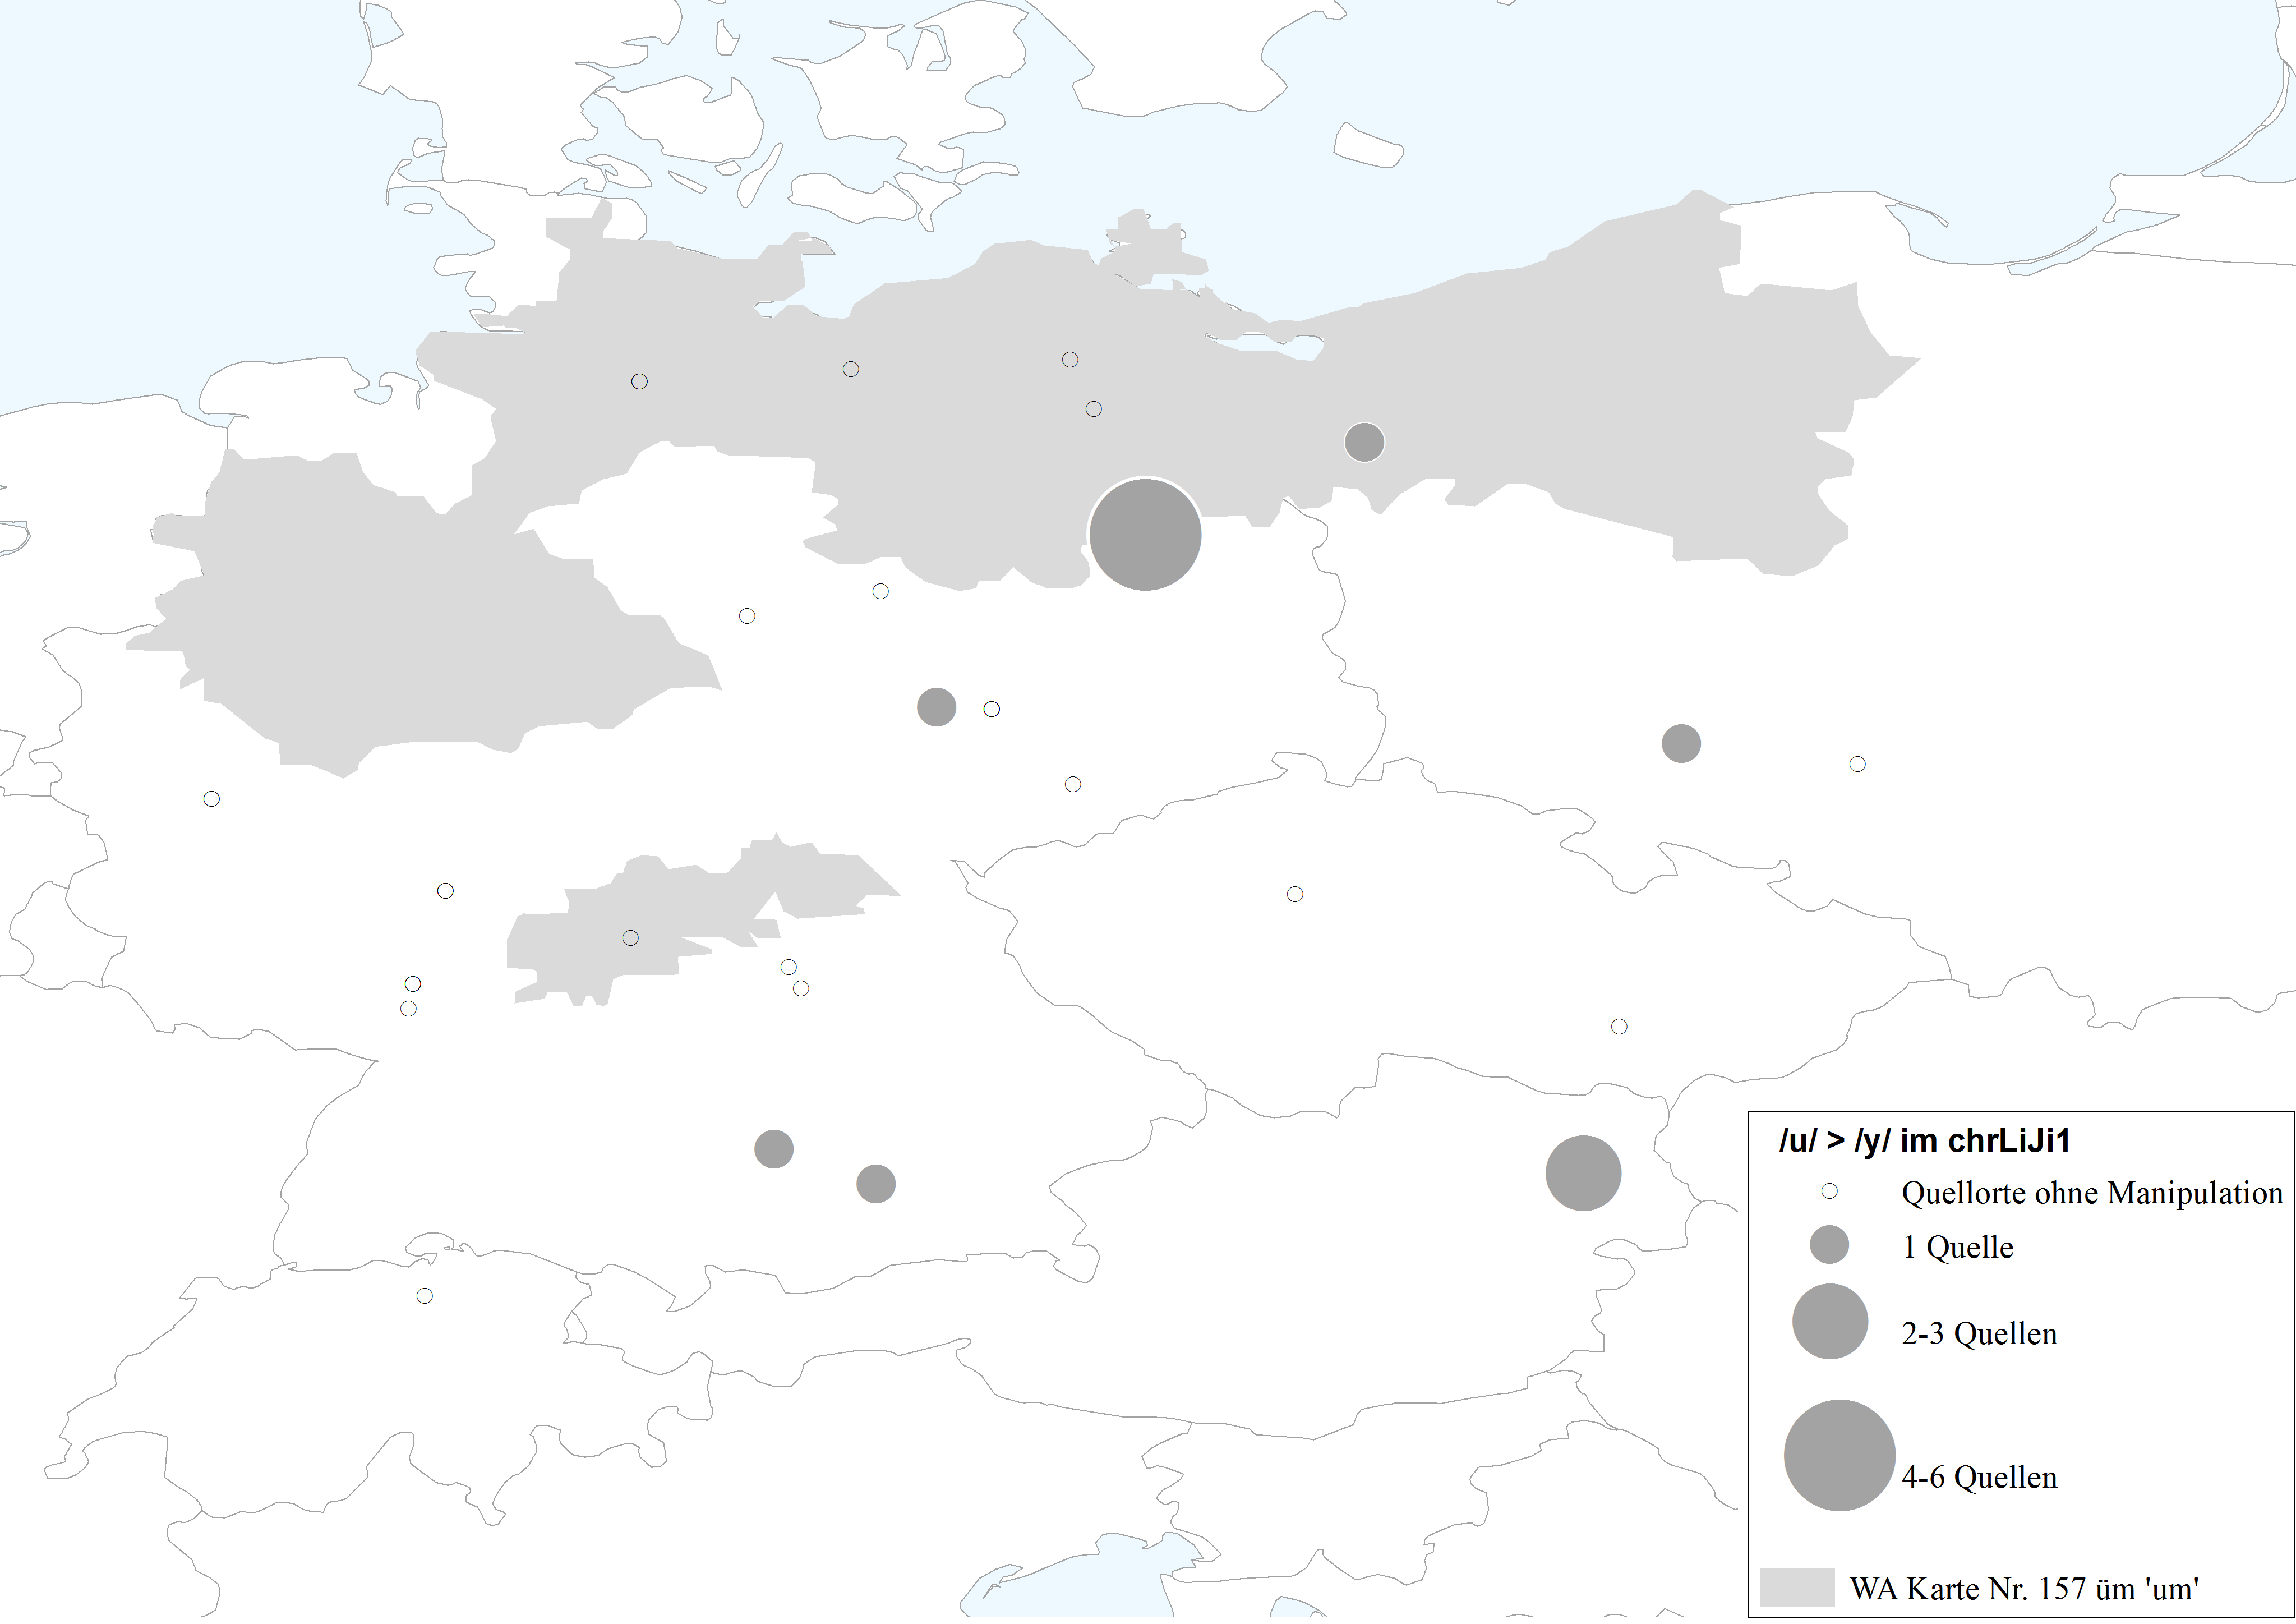
\includegraphics[width=\textwidth]{figures/palatkarte2.png}
		\caption{\label{kartepalat} \isi{Palatalisierung} von /\textit{u}(\textlengthmark)/ > /\textit{y}(\textlengthmark)/ im \hai{chrLiJi1} mit \hai{WA} Karte Nr. 157}
		\end{figure}

 
 
 Aufgrund fehlender Daten aus den westjiddischen Mundarten und insbesondere in Anbetracht der auffälligen geographischen Verteilung ist nicht mit Bestimmtheit zu entscheiden, ob wir es bei diesem Phänomen mit einer \quein{fehlerhaften} \isi{Imitation} des Jiddischen zu tun haben oder ob es an den entsprechenden Orten im Jiddischen tatsächlich präsent war, selbst wenn diese Präsenz nur durch angesiedelte Sprecher des \hai{{\SÜJ}} oder \hai{{\SOJ}} gegeben war. 
 
Als eine Bestätigung für die Hypothese, dass die \isi{Palatalisierung} im östlichen \hai{{\WJ}} Einzug gefunden hatte, könnten Belege derselben im \hai{jüdLiJi1} verstanden werden. Das \hai{jüdLiJi1}, dessen Quellen aus eben den östlichen Regionen stammen, in denen wir die \isi{Palatalisierung} im \hai{chrLiJi1} nachweisen konnten, zeigt dieses Phänomen in fünf Quellen.\footnote{Die da wären: \hai{GuS1}, \hai{GuS23}, \hai{PAlsleben}, \hai{PBerlin2} und \hai{PDebrecen}.} Im Fall der ungarischen Quelle \hai{PDebrecen} überrascht dies nicht, da wir hier eben jene Entwicklung aus dem Jiddischen kennen (vgl.\, \citealt{Hutterer1965};\citealt[83]{Herzog1992}). Anders ist es im Fall der sächsischen Quelle \hai{PAlsleben}, von wo die \isi{Palatalisierung}, von den oben angeführten Texten aus dem \hai{chrLiJi1}, von Leipzig abgesehen (Abbildung \ref{palat}), bislang nicht bekannt war.
 
    \section{Entrundungen (nhd. <ü>, <ö> > <i>, <e>)}\label{entrundung}
 %\noindent
Die hier als \isi{Entrundung} bezeichnete Entwicklung von {\mhd} \textit{u}, \textit{ü} zu /i/ und die weitergeführte Senkung zu /e/ fand z.\,T. bereits im Mitteljiddischen statt (\citealt[173f, 209–213]{Timm1987}). Der diachrone Ablauf des gesamten Prozesses, der im modernen \hai{{\OJ}} zum totalen Abbau der Umlaute von /u/ führte und auf den Abbau der Umlaute von /a/ und /o/ übergriff, ist jedoch noch ungeklärt. Anzunehmen ist, dass die \isi{Entrundung} in einzelnen Schüben einzelne Lexeme betraf (\textit{lexical diffusion}). So ist im modernen \hai{{\OJ}} {\mhd} \textit{u}, \textit{ü} zwar zumeist zu /i/ entrundet worden, z.\,B.\, in (\ref{bspentr1})–(\ref{bspentr4}). Zum Teil hat die \isi{Entrundung} aber auch zu einer weiteren Senkung geführt, wie etwa in (\ref{bspentr5}–\ref{bspentr7}) oder es blieb sogar der {\mhd} ungerundete Vokal erhalten  (\ref{bspentr8}–\ref{bspentr9}). Die \isi{Entrundung} hat so auch im späten \hai{{\WJ}} gewirkt (\ref{bspgrob12}–\ref{bspgrob11});\, bewirkte allerdings z.\,T. andere Folgeprozesse als im Standardostjiddischen, vgl.\, (\ref{bspentr8}) vs. (\ref{bspgrob14}). Die Präsenz der \isi{Entrundung} von {\mhd} \textit{u}, \textit{ü} im \hai{{\LiJi}} mag daher auf jiddische Sprachrealitäten fußen.
 
 
 
 \eenumsentence{
	\item {\oj} \RL{גליקלעך} \textit{gliklekh} \sem{glücklich} < {\mhd} \textit{gelücke}, \textit{glücke} \parencite[Bd. 1, Sp. 829]{Lexer1992} \label{bspentr1} 
	
	
	\item {\oj} \RL{טיר} \textit{tir} \sem{Tür} < {\mhd} \textit{Tür} \parencite[Bd. 2, Sp. 1579]{Lexer1992} \label{bspentr2}
	
	\item {\oj} \RL{קענען} \textit{kenen} \sem{können} < {\mhd} \textit{künnen}, \textit{kunnen} \parencite[Bd. 1, Sp. 1778]{Lexer1992} \label{bspentr3}
	
	\item {\oj}\RL{מעגן} \textit{megen} \sem{mögen} < {\mhd} \textit{mügen}, \textit{mugen} \parencite[Bd. 1, Sp. 2218]{Lexer1992} \label{bspentr4}
	
	\item {\oj} \RL{{פ\makebox(-0.8,9)[r]{\libertineGlyph{uni207B}}}א\makebox(-1.5,-7.5)[r]{\libertineGlyph{uni207B}}ר}
 \textit{far} \sem{für} < {\mhd} \textit{vür}, \textit{vüre} \parencite[Bd. 3, Sp. 583–585]{Lexer1992} \label{bspentr5}
 
 	\item {\oj} \RL{דא\makebox(-1.5,-7.5)[r]{\libertineGlyph{uni207B}}ר{פ\makebox(-0.8,9)[r]{\libertineGlyph{uni207B}}}ן} \textit{darfn} \sem{dürfen, brauchen} < {\mhd} \textit{dürfen}, \textit{durfen} \parencite[Bd. 1, Sp. 494]{Lexer1992} \label{bspentr6}
 
	 \item {\oj} \RL{דא\makebox(-1.5,-7.5)[r]{\libertineGlyph{uni207B}}ר} \textit{dar} \sem{dürr} < {\mhd} \textit{dürre}, \textit{durre} \parencite[Bd. 1, Sp. 497]{Lexer1992} \label{bspentr7}

	\item {\oj} \RL{מוזן} \textit{muzn} \sem{müssen} < {\mhd} \textit{müeʒen} (md. \textit{mûʒen} \textit{môʒen}) \parencite[Bd. 1, Sp. 2217]{Lexer1992}\label{bspentr8}
	
	\item  {\oj} \RL{קושן} \textit{kushn} \sem{küssen} < {\mhd} \textit{küssen} (md. \textit{kussen}) \parencite[Bd. 1, Sp. 1801]{Lexer1992}\label{bspentr9} 
	
	\item \RL{אונגליק} \textit{unglick} \sem{Unglück} (\qu{Die Hochzeit zu Grobsdorf} 1822:\,9)
\label{bspgrob12}

	\item \RL{מיזע} \textit{mizn} \sem{müssen} (\qu{Die Hochzeit zu Grobsdorf} 1822:\,u.\,a.\, 55)
\label{bspgrob14}

	\item \RL{קעננע} \textit{kenne} \sem{können} (\qu{Die Hochzeit zu Grobsdorf} 1822:\,10)
\label{bspgrob13}

	
	\item \RL{פאר} \textit{far} \sem{für} (\qu{Die Hochzeit zu Grobsdorf} 1822:\, u.\,a.\,19)
\label{bspgrob11} 
 

}\label{entrundungbsp}
 
 
Die jiddische Entwicklung findet allerdings ihre Parallelen in den deutschen Dialekten, wo die \isi{Entrundung} von {\mhd} \textit{u}, \textit{ü} und \textit{o}, \textit{ö} wie auch der Diphthonge \textit{öu}, \textit{üe} ab mittelhochdeutscher Zeit einsetzt und letzten Endes beinahe überall in unterschiedlicher Stärke wirksam wird, jedoch nirgends so konsequent, wie im \hai{{\OJ}}. Resistent blieben allein der Norden des Ripuarischen, das Ostfränkische inkl. des angrenzenden Thüringischen, das Schweizer, Bodensee- und Vorarlberger Alemannisch (mit Ausnahme des südlichen Höchstalemannischen) (\citealt[204–208]{Schirmunski1962}). Unter Umständen können damit auch die deutschen Dialekte in das \hai{{\LiJi}} hineingespielt haben.
 
 Im \hai{chrLiJi1} überwiegt deutlich die \isi{Entrundung} von <ü> > <i> (14 Quellen);\, Entrundungen von <ü> und <ö> zu <e> finden sich jeweils in 10 Quellen. Die Entrundungen von nhd. <ö> im \hai{chrLiJi1} beruhen zum einen auf einem Erhalt des {\mhd} Vokals \textit{ë}, z.\,B.\, in \textit{Lewenthaler} \sem{Löwenthaler} (\hai{FM} Leipzig, 1852:\,21, 28, 29, 31) < {\mhd} \textit{lëwe} \parencite[Bd. 1, Sp. 1893]{Lexer1992} oder stellen, was weitaus häufiger der Fall ist, eine Senkung von palatalisiertem {\germ} \textit{u} dar, etwa in \textit{mechten} \sem{möchten} (\hai{GW} n.a., ca.\, 1900:\,3, 4, 10;\, \hai{SS} Berlin, 1907:\,18;\, \hai{SV} München, 1890:\,1) < {\mhd} \textit{mügen, mugen} ({\ahd} \textit{mugan}) \parencite[Bd. 1, Sp. 2218]{Lexer1992}. Die \quein{einfache} \isi{Entrundung}, sprich eine nicht weiter gesenkte Form, liegt nur in einem Beleg vor: \textit{kinne} \sem{können} (\hai{PG} Speyer, 1835:\,34) < {\mhd} \textit{kunnen, künnen} \parencite[Bd. 1, Sp. 1778]{Lexer1992}. Diese Quelle ist auf den Ortspunkt Speyer zurückzuführen, wo im örtlichen deutschen Dialekt eben jene Form gebräuchlich ist (vgl.\, \hai{PfWB} \citeyear[Bd. 4, Sp. 445]{PfaelzWB}). Eine Interferenz aus dem Deutschen lässt sich demnach nicht ausschließen. 
 
 %%%\isi{Entrundung}%\begin{flushleft}	
\begin{figure}[b]
	\begin{tikzpicture}
		\begin{axis}[only marks, width=0.82\textwidth,height=0.2\textheight,
		legend style={at={(1,1)},xshift=+0.2cm, yshift=0cm,anchor=north west,nodes=left},
			%title={Funktionstypen des sp\"aten Westjiddisch},
			xtick={1700, 1725, 1750, 1775, 1800, 1825, 1850, 1875, 1900, 1925, 1950, 1975}, ytick=\empty,
			x tick label style={/pgf/number format/1000 sep=}, 
			y tick label style={/pgf/number format/1000 sep=},
			%extra y ticks={456.1, 1022.4},
			%extra y tick labels={{456,1},{1022,4}},
			extra y tick style={grid=major,
				tick label style={, ,}},
				ymin=0.4,
				ymax=3.1,
			ylabel={Phänomenbelege},
			enlarge x limits=0.03]	
	
			
			\addplot [mark=*, black] table [x=jahr, y=ue_i] {figures/ue_i.txt};%2.6
			\addplot [mark=*, gray] table [x=jahr, y=ue_e] {figures/ue_e.txt};%2.3
			\addplot [mark=square*, draw=black] table [x=jahr, y=oe_e] {figures/oe_e.txt};% 1.7
			\addplot [mark=square*,gray] table [x=jahr, y=oe_i] {figures/oe_i.txt};%1.4
			\addplot [mark=o,black] table [x=jahr, y=no] {figures/oe_i_no.txt};%1.1



			% Andere Formen a={mark=square*,blue},% b={mark=triangle*,red},% c={mark=o,draw=black}}
						\legend{<ü> als <i> , <ü> als <i>, <ö> als <e>, <ö> als <i>, unmanipuliert} %macht Legende
		\end{axis}
	\end{tikzpicture}
	\caption{Entrundungen im \hai{chrLiJi1}}
	\label{entrliji}	
\end{figure}

 
Zehn Korpustexte weisen mehrere Entrundungsstrategien auf, wie etwa <ö> > <e> und <ü> > <i>. Sie bleiben dabei aber konsequent lexemgebunden, d.\,h. wenn in einem Lexem nhd. <ü> als <i> gesetzt ist, dann wird dies konsequent beibehalten. In neun Quellen findet sich lediglich jeweils eine der vier möglichen Entrundungen. 


 Wir sehen im Histogramm (Abbildung \ref{entrliji}), dass Entrundungen von <ü> und <ö> (< {\mhd} \textit{ü}) erst zu einem späteren Stadium des \hai{chrLiJi1} auftreten. Ab den 1820er Jahren wird dieses Phänomen populär. In acht Quellen tritt die \isi{Entrundung} von <ü> neben der von <ö> auf.\footnote{Diese Quellen sind \hai{AK} (Zürich, 1948), \hai{GW} (n.a., ca.\, 1900), \hai{JP} (Altona, 1867), \hai{PA} (Frankfurt, 1834), \hai{SS} (Berlin, 1907), \hai{SV} (München, 1890), \hai{TH} (Merseburg, 1820) u. \hai{VD} (Frankfurt, 1916).}
 


Ein verhältnismäßig häufig entrundetes Lexem stellt \sem{für} > \textit{fer} dar. Es findet sich in fünf Quellen.\footnote{Die Quellen mit der \isi{Entrundung} von \sem{für} sind  \hai{AJ} (Berlin, 1825):\,2;\, \hai{GW} (n.a., ca.\, 1900):\,3,4,5;\, \hai{JK} (Breslau, 1810):\,13,20,42;\, \hai{PA} (Frankfurt, 1834):\,5;\, \hai{SV} (München, 1890):\,1,4,8,9.} Aus diesem Grund wird für die Vergleichskarte (Abbildung \ref{karteentrundung}) die \hai{WA}-Karte zu diesem Lexem herangezogen. Zuzüglich wurden Streubelege, \,%rs Spatium streichen
d.\,h. Belege die in der Kartierung Wenkers nicht unter Areale zusammengefasst wurden, zur \isi{Entrundung} von <i> am Lexem \sem{Stückchen} zu Arealen gebündelt und in die Kartierung in Abbildung \ref{karteentrundung} aufgenommen.\footnote{Wie in der Karte in Abbildung \ref{karteentrundung} zu sehen ist, sind diese Streubelege deutlich arealbildend. Der Umstand, dass die Wenkerkarten dies nicht erfassen, zeigt um ein weiteres, wie problematisch die Kartierungsmethoden Wenkers sind.} Vergleichskarten zur \isi{Entrundung} von nhd. <ö> konnten leider keine (brauchbaren)\footnote{Es gibt zwar eine halbe (!) Karte zu den Formen von \sem{könnt} (\hai{WA} Karte Nr. 384), doch diese deckt nur den nördl. Teil des Erhebungsgebiets ab.} herangezogen werden. Da die \isi{Entrundung} im beinahe gesamten deutschen Sprachgebiet gewirkt hat, sind die hier ausgewählten Lexeme und die sich daraus ergebenden Areale lediglich als Richtwert zu nehmen. Das sich damit ergebende Raumbild der \isi{Entrundung} im \hai{chrLiJi1} zeigt keine besonderen Auffälligkeiten, sei aber der Vollständigkeit halber hier angeführt (s. Abbildung \ref{karteentrundung}).


 \begin{figure}
 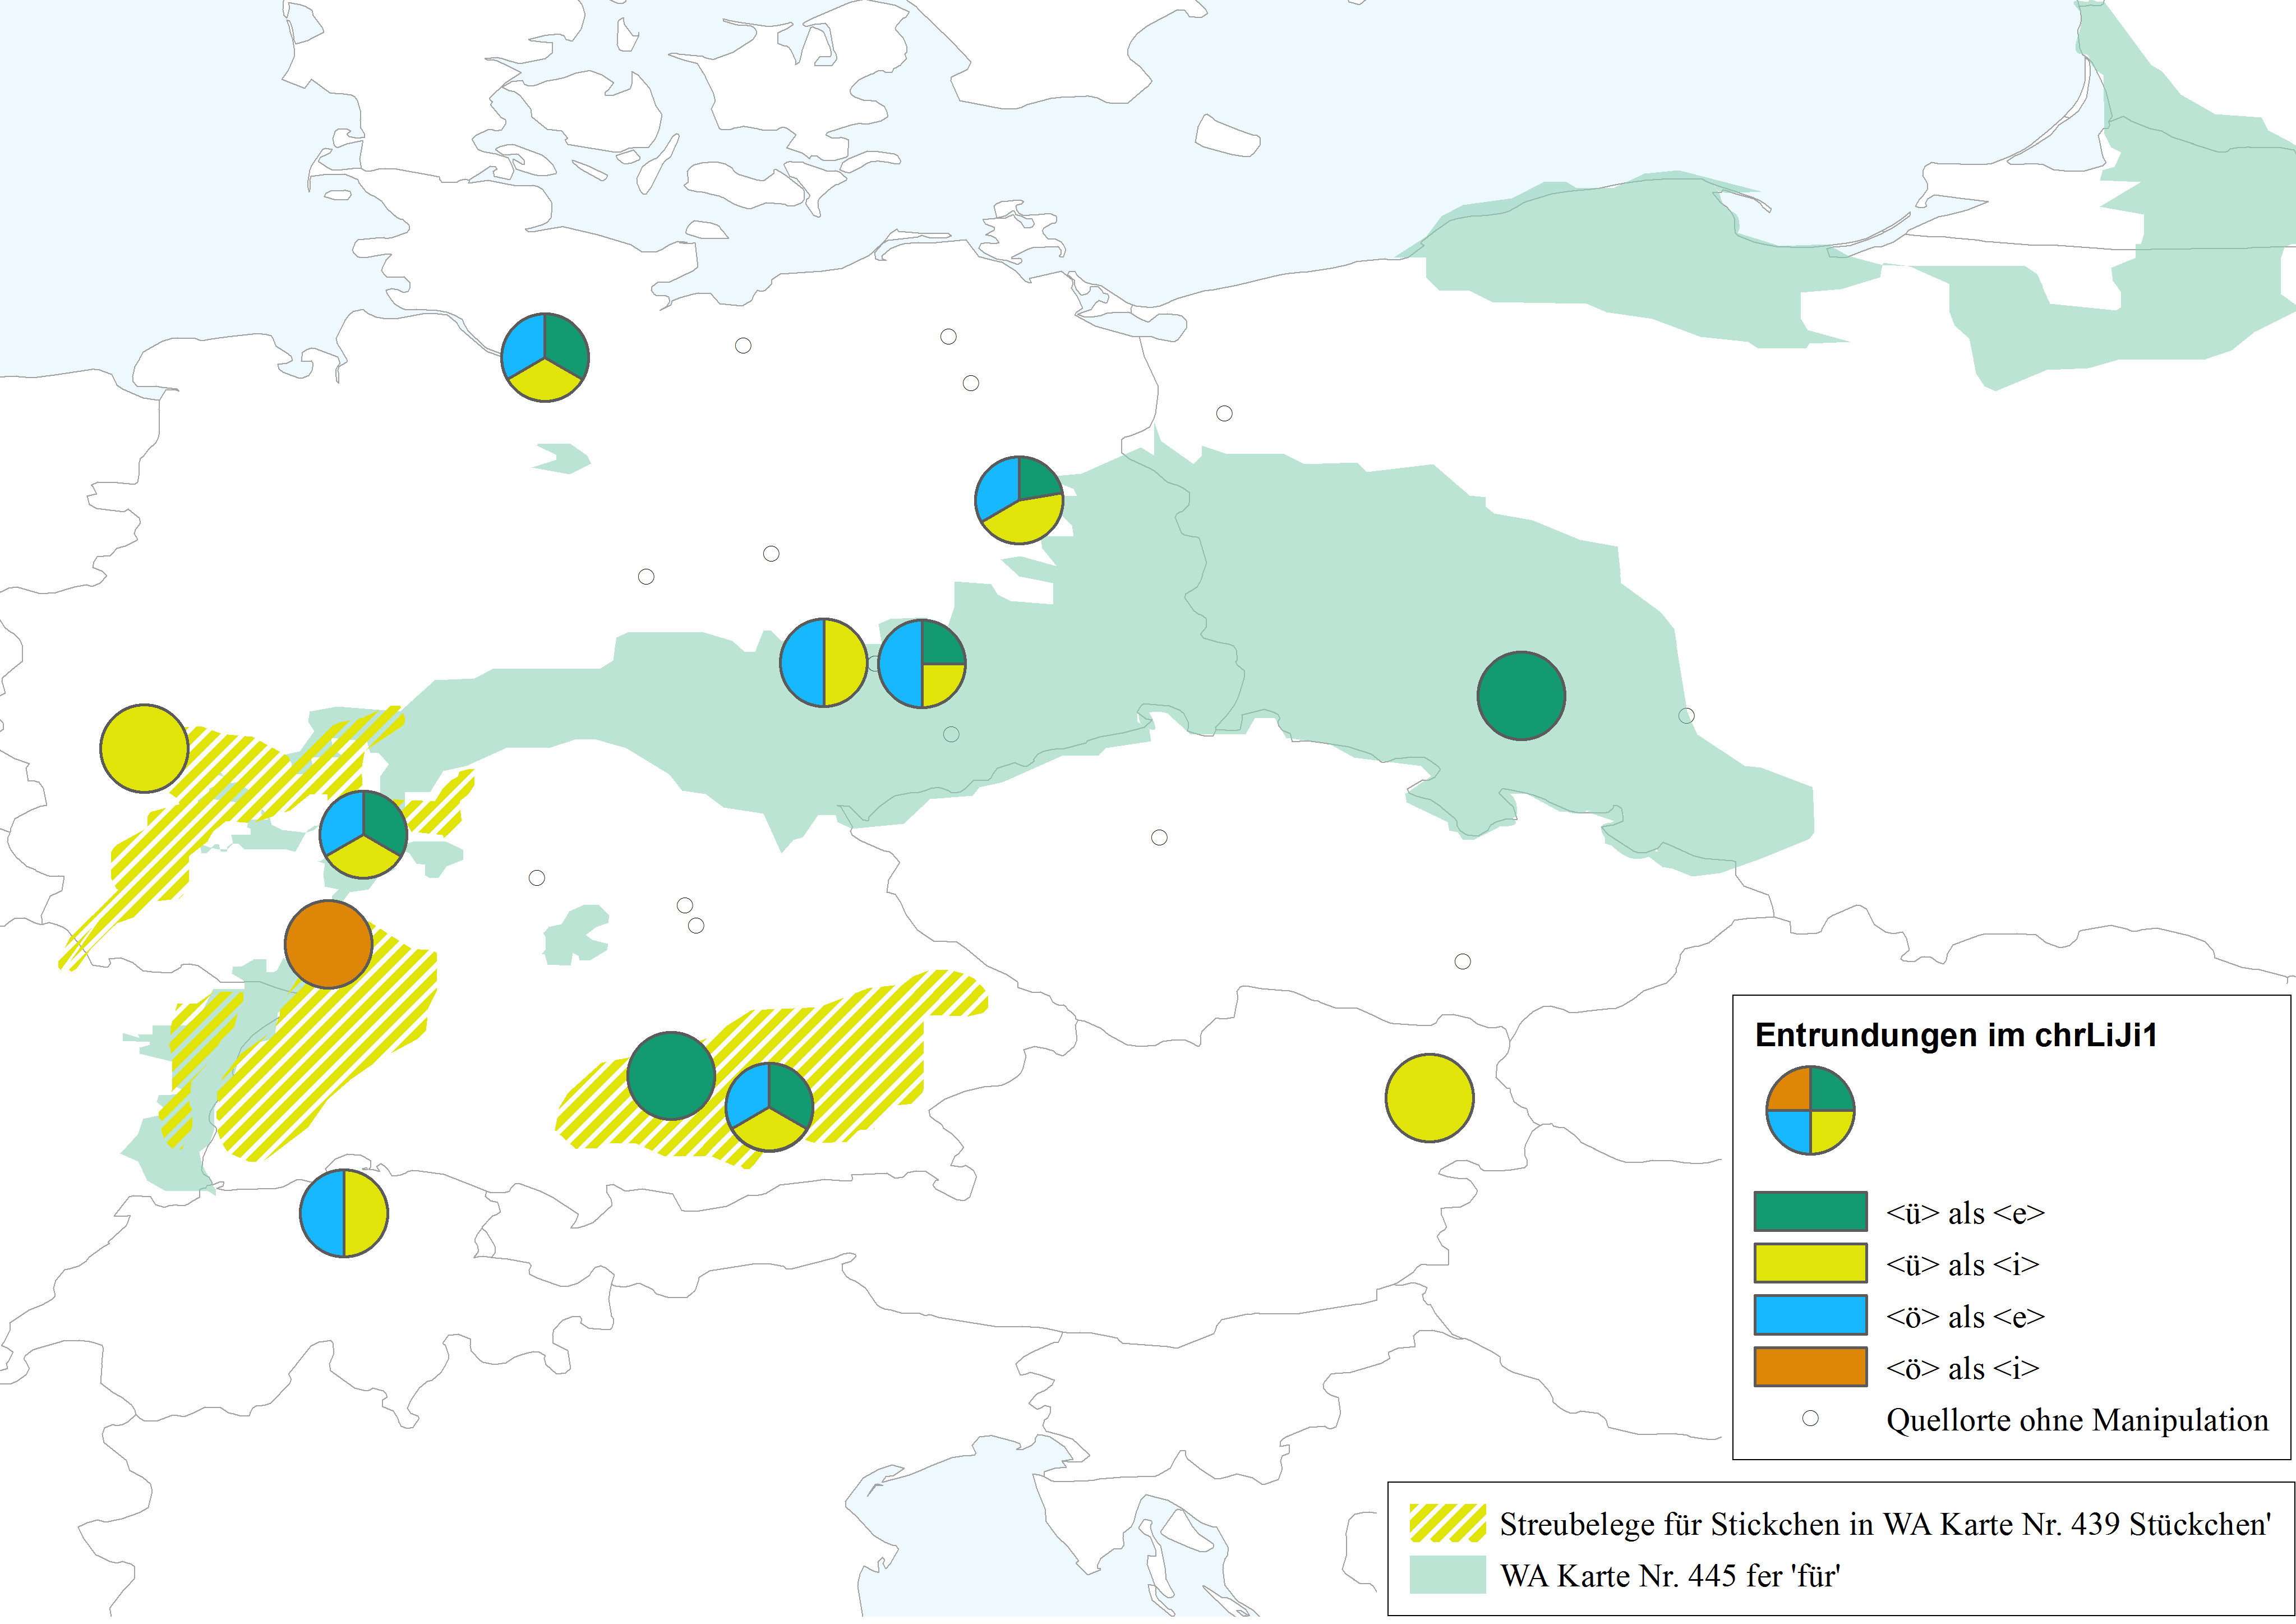
\includegraphics[width=\textwidth]{figures/entrundung_karte2.png}
		\caption{\label{karteentrundung} Entrundungen im \hai{chrLiJi1} mit \hai{WA} Karten Nr. 439 u. 445}
		\end{figure}

 
Das Subkorpus zum \hai{jüdLiJi1} zeigt in sechs Quellen die \isi{Entrundung} von <ü> zu <i>\footnote{Dies ist in den Quellen \hai{GuS10}, \hai{GuS23}, \hai{PAlsleben}, \hai{PBerlin2}, \hai{PBreslau} u. \hai{PDebrecen} der Fall.} und in fünf Quellen die von <ü> zu <e>\footnote{Gegeben in den Quellen \hai{GuS1}, \hai{GuS23}, \hai{PAlsleben}, \hai{PBerlin1} u. \hai{PBerlin2}.}. <ö> zu <e> findet sich in vier Quellen\footnote{In den Quellen \hai{GuS5}, \hai{GuS15}, \hai{PAlsleben} u. \hai{PDebrecen}.} und <ö> zu <i> in lediglich zwei Quellen der \hai{GuS}.\footnote{Zu finden in \hai{GuS1} u. \hai{GuS15}. In beiden Fällen findet sich lediglich das Lexem \sem{gönnen} zu \textit{ginnt} entrundet.} Auf lexikalischer Ebene finden sich zum \hai{chrLiJi1} marginale Unterschiede bei der Wahl der Lexeme, an denen entrundet wird. Ein direkter Unterschied zeigt die \isi{Entrundung} am Lexem \sem{für}. Während dieses im \hai{chrLiJi1} besonders zu \textit{fer} entrundet (s.\,o.), palatalisiert und gesenkt wurde, ist es im \hai{jüdLiJi1} der \hai{GuS} gesenkt als \textit{for} (\hai{GuS1}:\,5;\, \hai{GuS10}:\,5,6,7), in der ungarischen Quelle \hai{PDebrecen} als \textit{far} (\hai{PDebrecen}:\,5,6) und nur in einem Fall als \textit{fer} belegt (\hai{PAlsleben}:\,5).

 
Das generelle Bild zur \isi{Entrundung} zeigt, dass dies kein besonders häufiges Phänomen des \hai{{\LiJi}} ist. Die Tokenzahl zu diesem Phänomen ist auffällig gering. In der Regel wurden nur wenige, einzelne Lexeme einer \isi{Entrundung} unterzogen. Dass die \isi{Entrundung} nicht weiter als Mittel zur \isi{Imitation} des Jiddischen eingesetzt wurde, verwundert besonders, da das Fehlen der Umlaute von /a/, /u/ und /o/ im Jiddischen einen besonders starken Kontrast zum Schriftdeutschen darstellt und leicht als eine Regel wie etwa [{\textit{<ä>, <ü>, <ö> zu <e>}] umgesetzt werden könnte. Solche Hyperkorrekturen des Phänomens finden \,%rs finden
sich auch vereinzelt.
Die Autoren des \hai{{\LiJi}} müssen aber über das Wissen verfügt haben, dass die Entrundungen und besonders die daran geknüpften Senkungen im Jiddischen keinen synchron erkennbaren Gesetzmäßigkeiten folgen. Der Umstand, dass uns die \isi{Entrundung} von {\mhd} \textit{ü}, \textit{u} in den meisten Quellen sowohl als <e> wie auch als <i> in unterschiedlichen Lexemen parallel vorliegen, mag als Hinweis dafür gelten, dass die Autoren sich des komplexen Systems des Jiddischen bewusst waren und es nach bestem Wissen versucht haben umzusetzen. Auch dieses Phänomen spricht demnach gegen die landläufige Auffassung vom \hai{LiJi} als \quein{falsches Jiddisch} bzw. \quein{falsches Deutsch}.

\newpage 
  \section{Frikative}\label{frikative}
%\noindent 
Besonders auffällig verhalten sich die Graphien für Frikative im \hai{chrLiJi1}. Es finden sich die folgenden von der deutschen Schriftsprache abweichenden Graphien: <z> für <s>;\, <ß> für <s>;\, <ß> für <z>;\, <scht> für <st>. Diese werden im Folgenden einzeln besprochen. 

\subsection{Palatalisierung von <st> im An- und Auslaut}\label{scht}
%  %\noindent
Hinter der Schreibung <scht> für <st> verbirgt sich in seltenen Fällen die graphemische Umsetzung der in den hochdeutschen Varietäten wie auch im Jiddischen vollzogenen \isi{Palatalisierung} (bzw. Koronialisierung) von /sp/, /st/ > /ʃp/, /ʃt/ im \isi{Anlaut}, welche in der deutschen Schriftsprache im Fall als <sp> und <st> nicht \isi{ikonisch} ist, wie (\ref{bspscht2})–(\ref{bspscht3}) zeigen (vgl.\, \citealt[361]{Schirmunski1962};\citealt[365–368]{Bin-Nun1973};\citealt[272–277]{Timm1987};\citealt[§L 124]{Paul2007}).\footnote{Diese Entwicklung ist Teil einer \isi{Palatalisierung} von /s/ im \isi{Anlaut} vor /t/, /p/, /l/, /m/, /n/, /w/ und vereinzelt im \isi{Auslaut} nach /r/ (z.\,B.\, \textit{bars} > \textit{barsch}), die ab dem 13. Jahrhundert verschriftlicht belegt ist  \parencite[§L 124]{Paul2007}.} In nur einem Fall ist die hochdeutsche Aussprache verschriftlicht (\ref{bspscht1}). An diesem singulären Beleg  ist der Umstand interessant, dass es sich bei der Quelle um eine der wenigen niederdeutschen Quellen im Sample handelt. Hier bestand die besondere Notwendigkeit, die vom Niederdeutschen abweichende Aussprache zu verschriftlichen. Das Gros der Belege für diese graphematische Manipulationsstrategie findet sich im \hai{chrLiJi1} allerdings im \isi{Auslaut} (\ref{bspscht5b}), (\ref{bspscht5a}), (\ref{bspscht4}). Dabei finden sich z.\,T. Formen, die der ostjiddischen Aussprache entsprechen (\ref{bspscht5b}), ihr widersprechen (\ref{bspscht5a}) oder Germanismen, die im Ostjiddischen nicht gebräuchlich sind (\ref{bspscht4}). Die Graphie <scht> im \isi{Auslaut} ist in 12 Quelltexten gegeben. Belege für <scht> im Inlaut liegen nicht vor. 

 \eenumsentence{
 \item \textit{schteht} \sem{steht} (\hai{UT} Stavenhagen, 1862:\,Kap.\, 45);\, {\oj} \RL{שטיין} \textit{shteyn}
   \label{bspscht1}
 
 \item nhd. [ʃpiːl] <Spiel>, *<Schpiel>;\, {\oj} \RL{שפּיל} \textit{shpil}
 \label{bspscht2}
 
 \item nhd. [ʃtɪmə] <Stimme>, *<Schtimme>;\, {\oj} \RL{שטים} \textit{shtim}
 \label{bspscht3}
  
  \item \textit{Dorscht} \sem{Durst} (\hai{PG} Speyer, 1835:\,52);\, {\oj} \RL{ד{א\makebox(-1.25,-1.25)[r]{\libertineGlyph{uni05B8}}}רשט} \textit{dorsht}
 \label{bspscht5b}
 
  \item {\oj} \RL{רא\makebox(-1.5,-7.5)[r]{\libertineGlyph{uni207B}}שפייַל} \textit{rashpayl} \sem{Raspel} \label{bspspoj} %\parencite[409]{Weinreich2008}
  
 \item \textit{Krischt} \sem{Christ} (\hai{DK} Osterwieck, 1872:\,45);\, {\oj} \RL{קריסט} \textit{krist}
  \label{bspscht5a}
 
 
   \item \textit{Ferscht} \sem{Fürst} (\hai{VD} Frankfurt, 1916:\,15);\, keine {\oj} Entsprechung
 \label{bspscht4}



\item {\oj} \RL{דו ווייסט} \textit{du veyst} (*\textit{veysht}) \sem{du weist};vgl.\, {\aleman} \textit{wasch}\footnote{\label{fnalemannisch}Aleman. Sprachbeispiele sind vom Muttersprachler des Südvorarlberger Hochalemannischen (Bludenz) Oliver Schallert produziert. Der \textit{t}-Ausfall ist ein nach der \isi{Palatalisierung} von /st/ eintretendes Phänomen, das hier unberücksichtigt bleiben kann.}
\label{bspschtverb1}

\item {\oj} \RL{דו ה{א\makebox(-1.25,-1.25)[r]{\libertineGlyph{uni05B8}}}סט} \textit{du host} (*\textit{hosht}) \sem{du hast};vgl.\, {\aleman} \textit{hosch}\footnote{Wie Fn. \ref{fnalemannisch}.}
\label{bspschtverb2}

 }


Die Entwicklung im Aus- und Inlaut ist charakteristisch für die alemannischen (inkl. schwäbischen) und südrheinfränkischen Dialekte \parencite[361]{Schirmunski1962}. Ebenso ist dieses Phänomen für die mittel- und südbairischen Dialekte belegt. Hier ist es jedoch lexemgebunden und nicht systematisch wie im Alemannischen durchgeführt (vgl.\, \hai{TSA2} Karten Nr. 16, 51;\,  \hai{KDSA} Karten Nr. 153–159). Auch das Jiddische zeigt dieses Phänomen in Aus- und Inlaut (\ref{bspscht5b})–(\ref{bspspoj}). Es gibt aber auch Fälle, in denen der Alveolar vor /t/ und /p/ erhalten bleibt, wie etwa in (\ref{bspscht5a}) oder in der Verbflexion (\ref{bspschtverb1})–(\ref{bspschtverb2}). Das Jiddische folgt damit einer anderen Systematik als die deutschen Dialekte. Die historische Situation ist besonders schwer zu beschreiben, da \RL{<ש>} in der Regel unpunktiert bleibt und damit sowohl den alveolaren wie auch den postalveolaren \isi{Frikativ} bezeichnen kann (vgl.\, \citealt[153, 272]{Timm1987}). 

Die Verteilung der <scht>-Graphie im \hai{chrLiJi1} in Abbildung \ref{<scht>} zeigt, dass diese Manipulationsstrategie nur punktuell verwendet wurde.

  %%%<scht> Diagramm%\begin{flushleft}	
\begin{figure}
	\begin{tikzpicture}
		\begin{axis}[only marks, width=0.82\textwidth,height=0.2\textheight,
		legend style={at={(1,1)},xshift=+0.2cm, yshift=-0.34cm,anchor=north west,nodes=left},
			%title={Funktionstypen des sp\"aten Westjiddisch},
			xtick={1700, 1725, 1750, 1775, 1800, 1825, 1850, 1875, 1900, 1925, 1950, 1975}, ytick=\empty,
			x tick label style={/pgf/number format/1000 sep=}, 
			y tick label style={/pgf/number format/1000 sep=},
			%extra y ticks={456.1, 1022.4},
			%extra y tick labels={{456,1},{1022,4}},
			extra y tick style={grid=major,
				tick label style={, ,}},
				ymin=0.7,
				ymax=2.9,
			ylabel={Phänomenbelege},
			enlarge x limits=0.03]	
	
			
\addplot [mark=*, black] table [x=jahr, y=scht_auslaut] {figures/scht.txt};%2.3
\addplot [mark=*, gray] table [x=jahr, y=scht_anlaut] {figures/scht_anlaut.txt};%1.8
\addplot [mark=o, black] table [x=jahr, y=no] {figures/scht_no.txt};%1.3

						\legend{<scht> \isi{Auslaut},<scht> \isi{Anlaut},unmanipuliert} 
		\end{axis}
	\end{tikzpicture}
	\caption{<scht> im \hai{chrLiJi1}}
	\label{<scht>}	
\end{figure}



Da der postalveolare \isi{Frikativ} /ʃ/ im \isi{Auslaut} vor /p/ und /t/ besonders im Südwesten des deutschen Dialektraums verbreitet ist (s.\,o.), wäre anzunehmen, dass die dieses Phänomen verwendenden Quellen aus eben jener Region stammen oder aus dem niederdeutschen Raum, wo das Jiddische besonders mit seinen hochdeutschen Eigenschaften auffiel. Die räumliche Verteilung zeigt, dass immerhin sieben der zwölf Quellen, welche <scht> im \isi{Auslaut} zeigen, im oder zumindest in nächster Nähe zum Areal liegen, in dem diese \isi{Koronalisierung} in den deutschen Dialekten stattfand (s. Abbildung \ref{kartescht}).\footnote{Wie bei allen Karten des \hai{WA} sind die zum  Zeitpunkt der ersten Wenkererhebungem noch nicht gewonnenen Daten zur Schweiz, Liechtenstein und Österreich nicht im Kartenbild präsent. Man muss sich hier das \textit{fescht}-Areal als nach Süden hin verlängert denken (vgl.\, \citealt[361]{Schirmunski1962}). Bei den Orten Frankfurt und Wien sind jeweils zwei Quellen am Ort gegeben, in denen <scht> im \isi{Auslaut} verwendet wird.} Die übrigen fünf Quellen verteilen sich entlang des Grenzraums zwischen Ost- und \ili{Westjiddisch}. Hier könnte also der Kontakt zum \hai{{\OJ}} eine Rollen gespielt haben.

\begin{figure}
		\centering
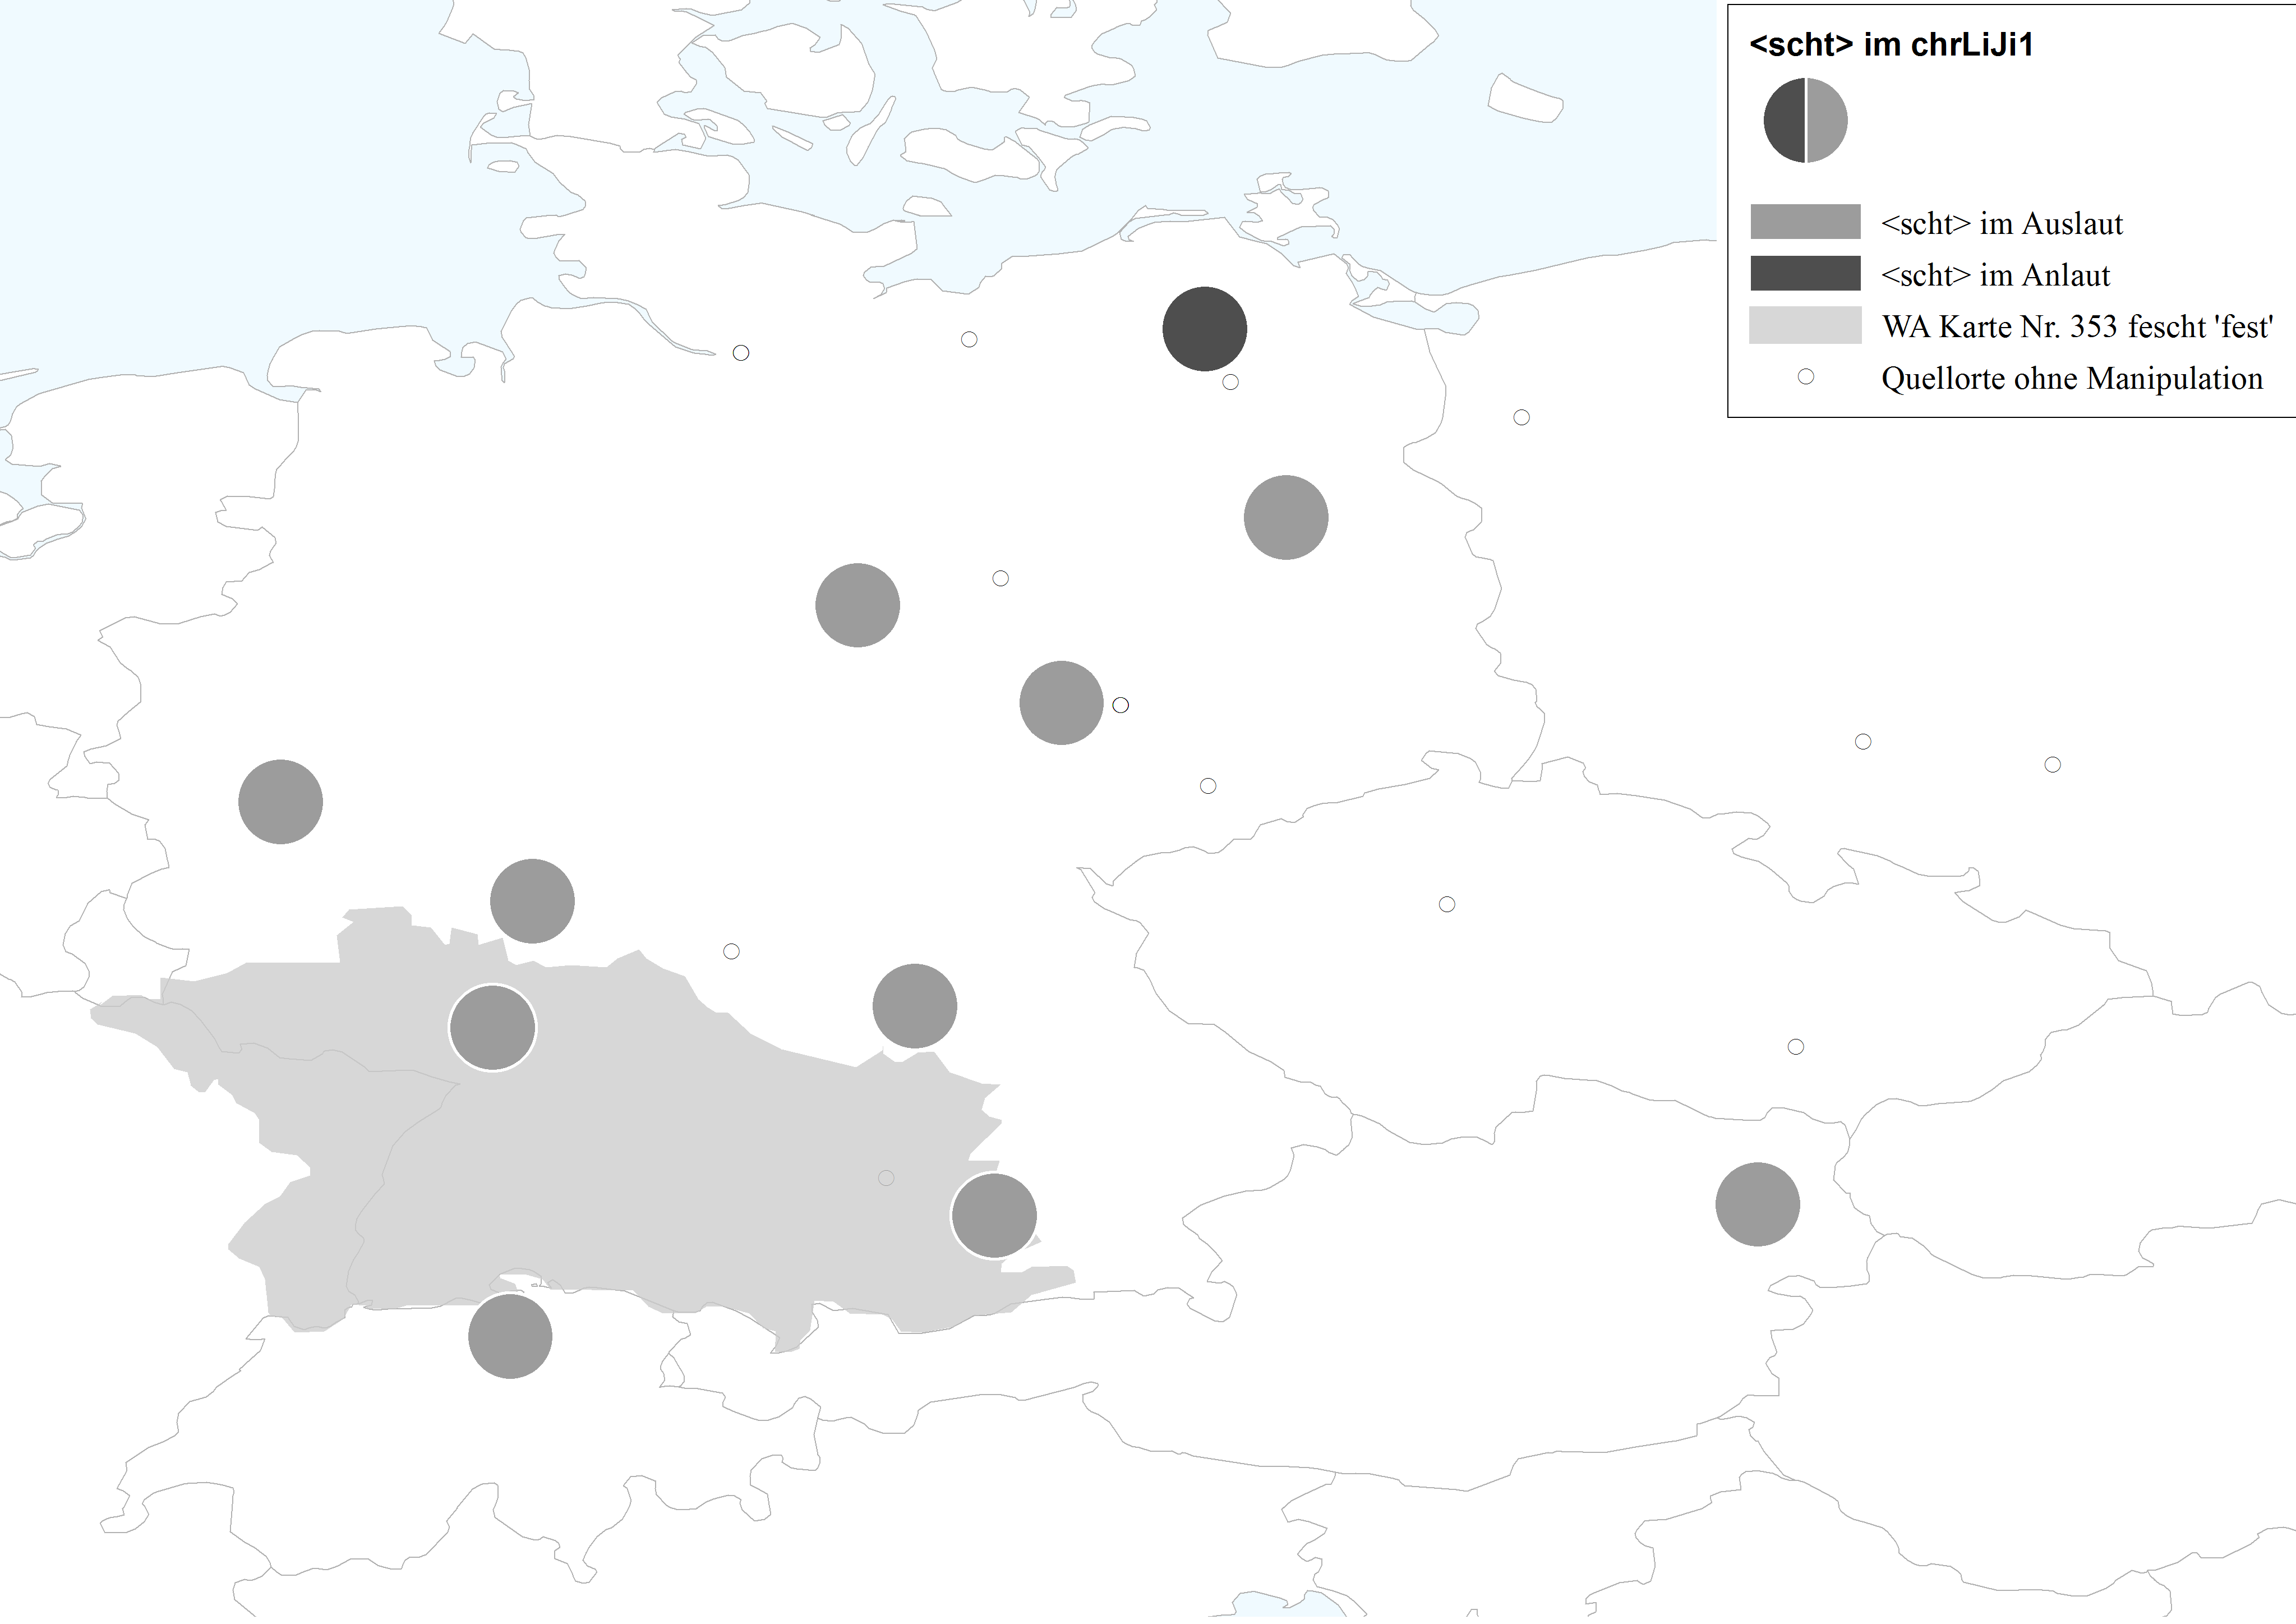
\includegraphics[width=\textwidth]{figures/scht_karte.png}
		\caption{\label{kartescht} <scht> im \hai{chrLiJi1} mit \hai{WA} Karten Nr. 353}
		\end{figure}

% \todo{Karte vor/nach Beispielen; nicht zwischen drin}

Die Belege aus dem Südwesten müssen aber nicht zwangsläufig Interferenzen zwischen \hai{{\LiJi}} und den deutschen Dialekten sein, sondern können auch die tatsächliche Situation im örtlichen Westjiddischen erfassen. Zumindest zeigen die letzten Tonaufnahmen von Sprechern des \hai{{\SWJ}} aus dem alemannischen Sprachgebiet der späten 50er und 60er Jahre eben dieses Phänomen, wie etwa in (\ref{bspschtalem1})–(\ref{bspschtalem2b}).

\largerpage
 \eenumsentence{
 
 \item \textit{faʃtə} \sem{Fasten} (Endinger \hai{{\SWJ}};\citealt[74]{Fleischer2005})
 \label{bspschtalem1}

 \item \textit{luʃtig} \sem{lustig} (Endinger \hai{{\SWJ}};\citealt[74]{Fleischer2005})
 \label{bspschtalem1b}
 
 \item \textit{iʃ} \sem{ist} (Grussenheim,\, Oberelsass;\, \citealt[43]{GuggenheimGruenberg1966})
 \label{bspschtalem2}
 
 \item {\sloppy \textit{maiʃti} \sem{meisten} (Grussenheim,\, Oberelsass;\, \citeauthor{GuggenheimGruenberg1966}\\ \citeyear*{GuggenheimGruenberg1966}:43)
}
 \label{bspschtalem2b} 
 
 
 }
 
\largerpage
Man könnte nun annehmen, dass diese Formen im \hai{{\SWJ}} auf den starken \isi{Sprachkontakt} zum Alemannischen schließen, welcher besonders stark v.\,a.\, auf morphosyntaktischer Ebene auf das Jiddische gewirkt hat (vgl.\, \citealt{Schaefer2014}). Doch Belege aus anderen Regionen zeigen, dass die \isi{Palatalisierung} nicht zwangsläufig auf den alemannischen \isi{Sprachkontakt} zurückzuführen ist, sondern auch ein autochthon jiddisches Phänomen ist,\,  s.\, Bsp.\,  in (\ref{bspwjscht}). \cite[98f]{GuggenheimGruenberg1958}, \cite[20]{Beem1970} und Beraneks \hai{WjSA} (Karte Nr. 39) gehen davon aus, dass die \isi{Palatalisierung} im In- und \isi{Auslaut} im gesamten \hai{{\WJ}}, mit Ausnahme des östl. \hai{{\NWJ}}, vollzogen wurde;\, jedoch liegen kaum Analysen zur Systematik dieses Phänomens vor. Im \hai{ZWJ} der \qu{Hochzeit zu Grobsdorf} etwa findet sich \RL{<שט>} im In- und \isi{Auslaut} (\ref{bspgrob20})–(\ref{bspgrob22});\, in deutschsprachigen Sequenzen bzw. auf dem Titelblatt findet sich hingegen \RL{<סט>} gesetzt (\ref{bspgrob23}). \RL{<שט>} steht allerdings nie nach Nasal (\ref{bspgrob24})–(\ref{bspgrob25}). Darin verhält sich der Text äußerst homogen. Auch das \hai{{\NWJ}} Aurichs zeigt, in unmissverständlicher lateinischer \isi{Orthographie}, dieses Phänomen (\ref{bspaurich1})–(\ref{bspaurich2}). Anders als im \hai{{\OJ}}  (\ref{bspschtverb1})–(\ref{bspschtverb2}), findet sich die Koronialisierung in der hessischen Quelle auch bei Verben, z.\,B.\, (\ref{bspgrob25}).  Eine  Systematik wie im \hai{{\OJ}} oder im \hai{{\WJ}} der \qu{Hochzeit zu Grobsdorf} gegeben, lässt sich im \hai{{\LiJi}} jedoch nicht erkennen. Nirgends im \hai{{\WJ}} ist aber die \isi{Palatalisierung} von /st/ im In- und \isi{Auslaut} dermaßen konsequent durchgeführt, wie im westl. \hai{{\SWJ}};der alemannische Einfluss mag hier also gewirkt haben.

   \eenumsentence{
 \item  \RL{לושטיג}  \textit{lusshtig} \sem{lustig} (\qu{Die Hochzeit zu Grobsdorf} 1822:\,10) 
\label{bspgrob20} 

 \item  \RL{ערשט} \textit{erscht} \sem{erst} (\qu{Die Hochzeit zu Grobsdorf} 1822:\,8, 12, 14)
\label{bspgrob21} 

 \item  \RL{ווא\makebox(-1.5,-7.5)[r]{\libertineGlyph{uni207B}}רשטע} \textit{varshte} \sem{wirst du} (\qu{Die Hochzeit zu Grobsdorf} 1822:\,27)
\label{bspgrob22} 

\item  \RL{לוסטיג} (im dt. Text) \textit{lustig} (\qu{Die Hochzeit zu Grobsdorf} 1822:\,Titel,\,  32) \label{bspgrob23} 
 
 \item \RL{זונסט} \textit{zunst} \sem{sonst} (\qu{Die Hochzeit zu Grobsdorf} 1822:\,12, 13, 14, 27)
\label{bspgrob24} 

 \item  \RL{קומסט} \textit{kumst} \sem{kommst} (\qu{Die Hochzeit zu Grobsdorf} 1822:\, u.\,a.\, 8)
\label{bspgrob25} 

\item \textit{geschtern} \sem{gestern} \parencite[125]{Reershemius2007}
\label {bspaurich1}
 
\item \textit{erscht} 
\sem{erst} \parencite[125]{Reershemius2007}
\label {bspaurich2}

\item \textit{nischt} \sem {nicht} (A.H. Heymann \qu{Lebenserinnerungen} 1909:\,5)
 
 }\label{bspwjscht}

Damit ist schwer zu entscheiden, ob in die südwestlichen Quellen des  \hai{chrLiJi1} Formen deutscher Dialekte in die \isi{Imitation} einflossen, oder ob die tatsächlich westjiddische Form durch den Umstand, dass die \isi{Assimilation} von /st/ an diesen Orten allgegenwärtig war, leichter für die Imitatoren zugänglich war, als andernorts.

Im \hai{jüdLiJi1} tritt die Schreibung <scht> nur sehr selten in Erscheinung. In fünf Texten findet sie sich im Aus- und Inlaut.\footnote{Die entsprechenden Quellen sind \hai{GuS5}, \hai{GuS23}, \hai{PAlsleben}, \hai{PBerlin1} u. \hai{PBerlin2}.} Insbesondere ist hier das Lexem \sem{erste} betroffen, welches in drei Quellen\footnote{\hai{GuS5}, \hai{PAlsleben} u. \hai{PBerlin1}.} die einzige Manipulation zu <scht> aufweist. Eine Quelle, \hai{PBerlin2}, legt besonderen Wert darauf, die hochdeutsche bzw. jiddische Aussprache im \isi{Anlaut} zu verschriftlichen;\, sonst spielt diese keine Rolle im \hai{jüdLiJi1}. Es irritiert, dass \hai{jüdLiJi1} hier scheinbar weniger authentisch ist, als das \hai{chrLiJi1}.


Selbst, wenn dieses Phänomen nicht zu den frequentesten Manipulationsstrategien des \hai{{\LiJi}} zählt, so zeigt es doch um ein Weiteres, dass \hai{chrLiJi1} auf phonologischer Ebene näher an der tatsächlichen Sprachrealität des \hai{{\WJ}} ist als \hai{jüdLiJi1}. Dieses Bild kann natürlich der Unausgewogenheit des kleinen \isi{Korpus} geschuldet sein. Dass uns aber kaum Belege für die \isi{Palatalisierung} von /st/ im In- und \isi{Auslaut} aus dem kleineren \isi{Korpus} vorliegen, darf als Indiz dafür gelten, dass deren Konzepte von literarischem Jiddisch andere Prioritäten setzen als das \hai{chrLiJi1}. 

\subsection{Koronalisierung <ch> > <sch>}\label{ch}
%  %\noindent
Elf Texte des \hai{chrLiJi1} verwenden die \isi{Koronalisierung} von /ҫ/ <ch> zu /ʃ/ <sch>  im Lexem \sem{nicht} < {\mhd} \textit{niht} \parencite[Bd. 2, Sp. 83]{Lexer1992}. Hier fällt besonders die lexematische Gebundenheit der \isi{Imitation} auf. Die \isi{Koronalisierung} wurde scheinbar nicht als Regel erkannt, sondern nur als Alternativform eines Lexems.  

Die diachrone Verteilung der Quellen mit einer Verschriftlichung der \isi{Koronalisierung} von /ҫ/ zu /ʃ/ zeigt, dass diese erst ab dem 19. Jahrhundert ins \hai{chrLiJi1} Eingang findet (s. Histogramm in Abbildung \ref{histoch}).


    %%%V12/13Diagramm%\begin{flushleft}	
\begin{figure}
	\begin{tikzpicture}
		\begin{axis}[only marks, width=0.82\textwidth,height=0.2\textheight,
		legend style={at={(1,1)},xshift=+0.2cm, yshift=-0.7cm,anchor=north west,nodes=left},
			%title={Funktionstypen des sp\"aten Westjiddisch},
			xtick={1700, 1725, 1750, 1775, 1800, 1825, 1850, 1875, 1900, 1925, 1950, 1975}, ytick=\empty,
			x tick label style={/pgf/number format/1000 sep=}, 
			y tick label style={/pgf/number format/1000 sep=},
			%extra y ticks={456.1, 1022.4},
			%extra y tick labels={{456,1},{1022,4}},
			extra y tick style={grid=major,
				tick label style={, ,}},
				ymin=0.7,
				ymax=2.9,
			ylabel={Phänomenbelege},
			enlarge x limits=0.03]	
	
			
\addplot [mark=*, black] table [x=jahr, y=ch] {figures/ch.txt};%2

\addplot [mark=o, black] table [x=jahr, y=no] {figures/ch_no.txt};%1.5


 

			% Andere Formen a={mark=square*,blue},% b={mark=triangle*,red},% c={mark=o,draw=black}}
						\legend{\textit{nischt}, unmanipuliert} %macht Legende
		\end{axis}
	\end{tikzpicture}
	\caption{\isi{Koronalisierung} von \sem{nicht} im \hai{chrLiJi1}}
	\label{histoch}	
\end{figure}

  
Ausnahmsweise wurde für die geographische Darstellung eine Karte aus dem umstrittenen\footnote{Vgl. \textcite{GuggenheimGruenberg1966b} bzw. \textcite{GuggenheimGruenberg1968}.} \hai{WjSA} von Beranek angeführt, da hier eine interessante Vergleichskarte zum Lexem \sem{nicht} vorliegt (s. Abbildung \ref{kartenischt}). Nach Beranek findet sich \textit{nischt} vom \hai{{\NÜJ}} bis ins östl. \hai{{\NWJ}} hinein, für das restliche Gebiet des \hai{{\WJ}} gibt Beranek \textit{niks} als die vorherrschende Form an. Im \hai{{\OJ}} ist sowohl \RL{נישט} \textit{nisht} wie auch \hai{ניט} \textit{nit} verbreitet. Nach \cite[375]{Bin-Nun1973} gestaltet sich die areale Verbreitung so, dass die nicht-koronalisierten Formen \textit{niks} im \hai{{\SÜJ}} und \textit{nit} im \hai{{\NOJ}} auftreten, \textit{nischt} hingegen im restlichen Teil des \hai{{\WJ}} sowie in \hai{{\ZOJ}} und \hai{{\SOJ}}. 

Im Deutschen hat sich eine vergleichbare \isi{Koronalisierung} erst im 19. Jahrhundert ausgehend von Stadtmundarten im Westen des Sprachgebiets,   herausgebildet \parencite[97–101]{Herrgen1986}. Im Rhein- und Moselfränkischen und Ripuarischen ist /ҫ/ mit  [ʒ] konsequent zusammengefallen (\citealt[275]{Schirmunski1962}; \citealt{Herrgen1986}). Eine solche Regelmäßigkeit der \isi{Koronalisierung}, wie auch eine Entwicklung zu  [ʒ], liegt im Ost- wie Westjiddischen nicht vor. Das Lexem \sem{nicht} stellt eine Ausnahme dar. Neben den fränkischen Dialekten ist die Form \textit{nischt} auch für das Osthessische und Obersächsische beschrieben (\hai{DWB} \citeyear[Bd. 13, Sp. 729]{DeutschesWB}). Im Wenkeratlas zeigt sich die \isi{Koronalisierung} weit im Ostmitteldeutschen und den Mundarten der nordostdeutschen Siedlungsmundarten (vgl.\, \hai{WA} Karte Nr. 537 \sem{nichts}).

 \begin{figure}
		\centering
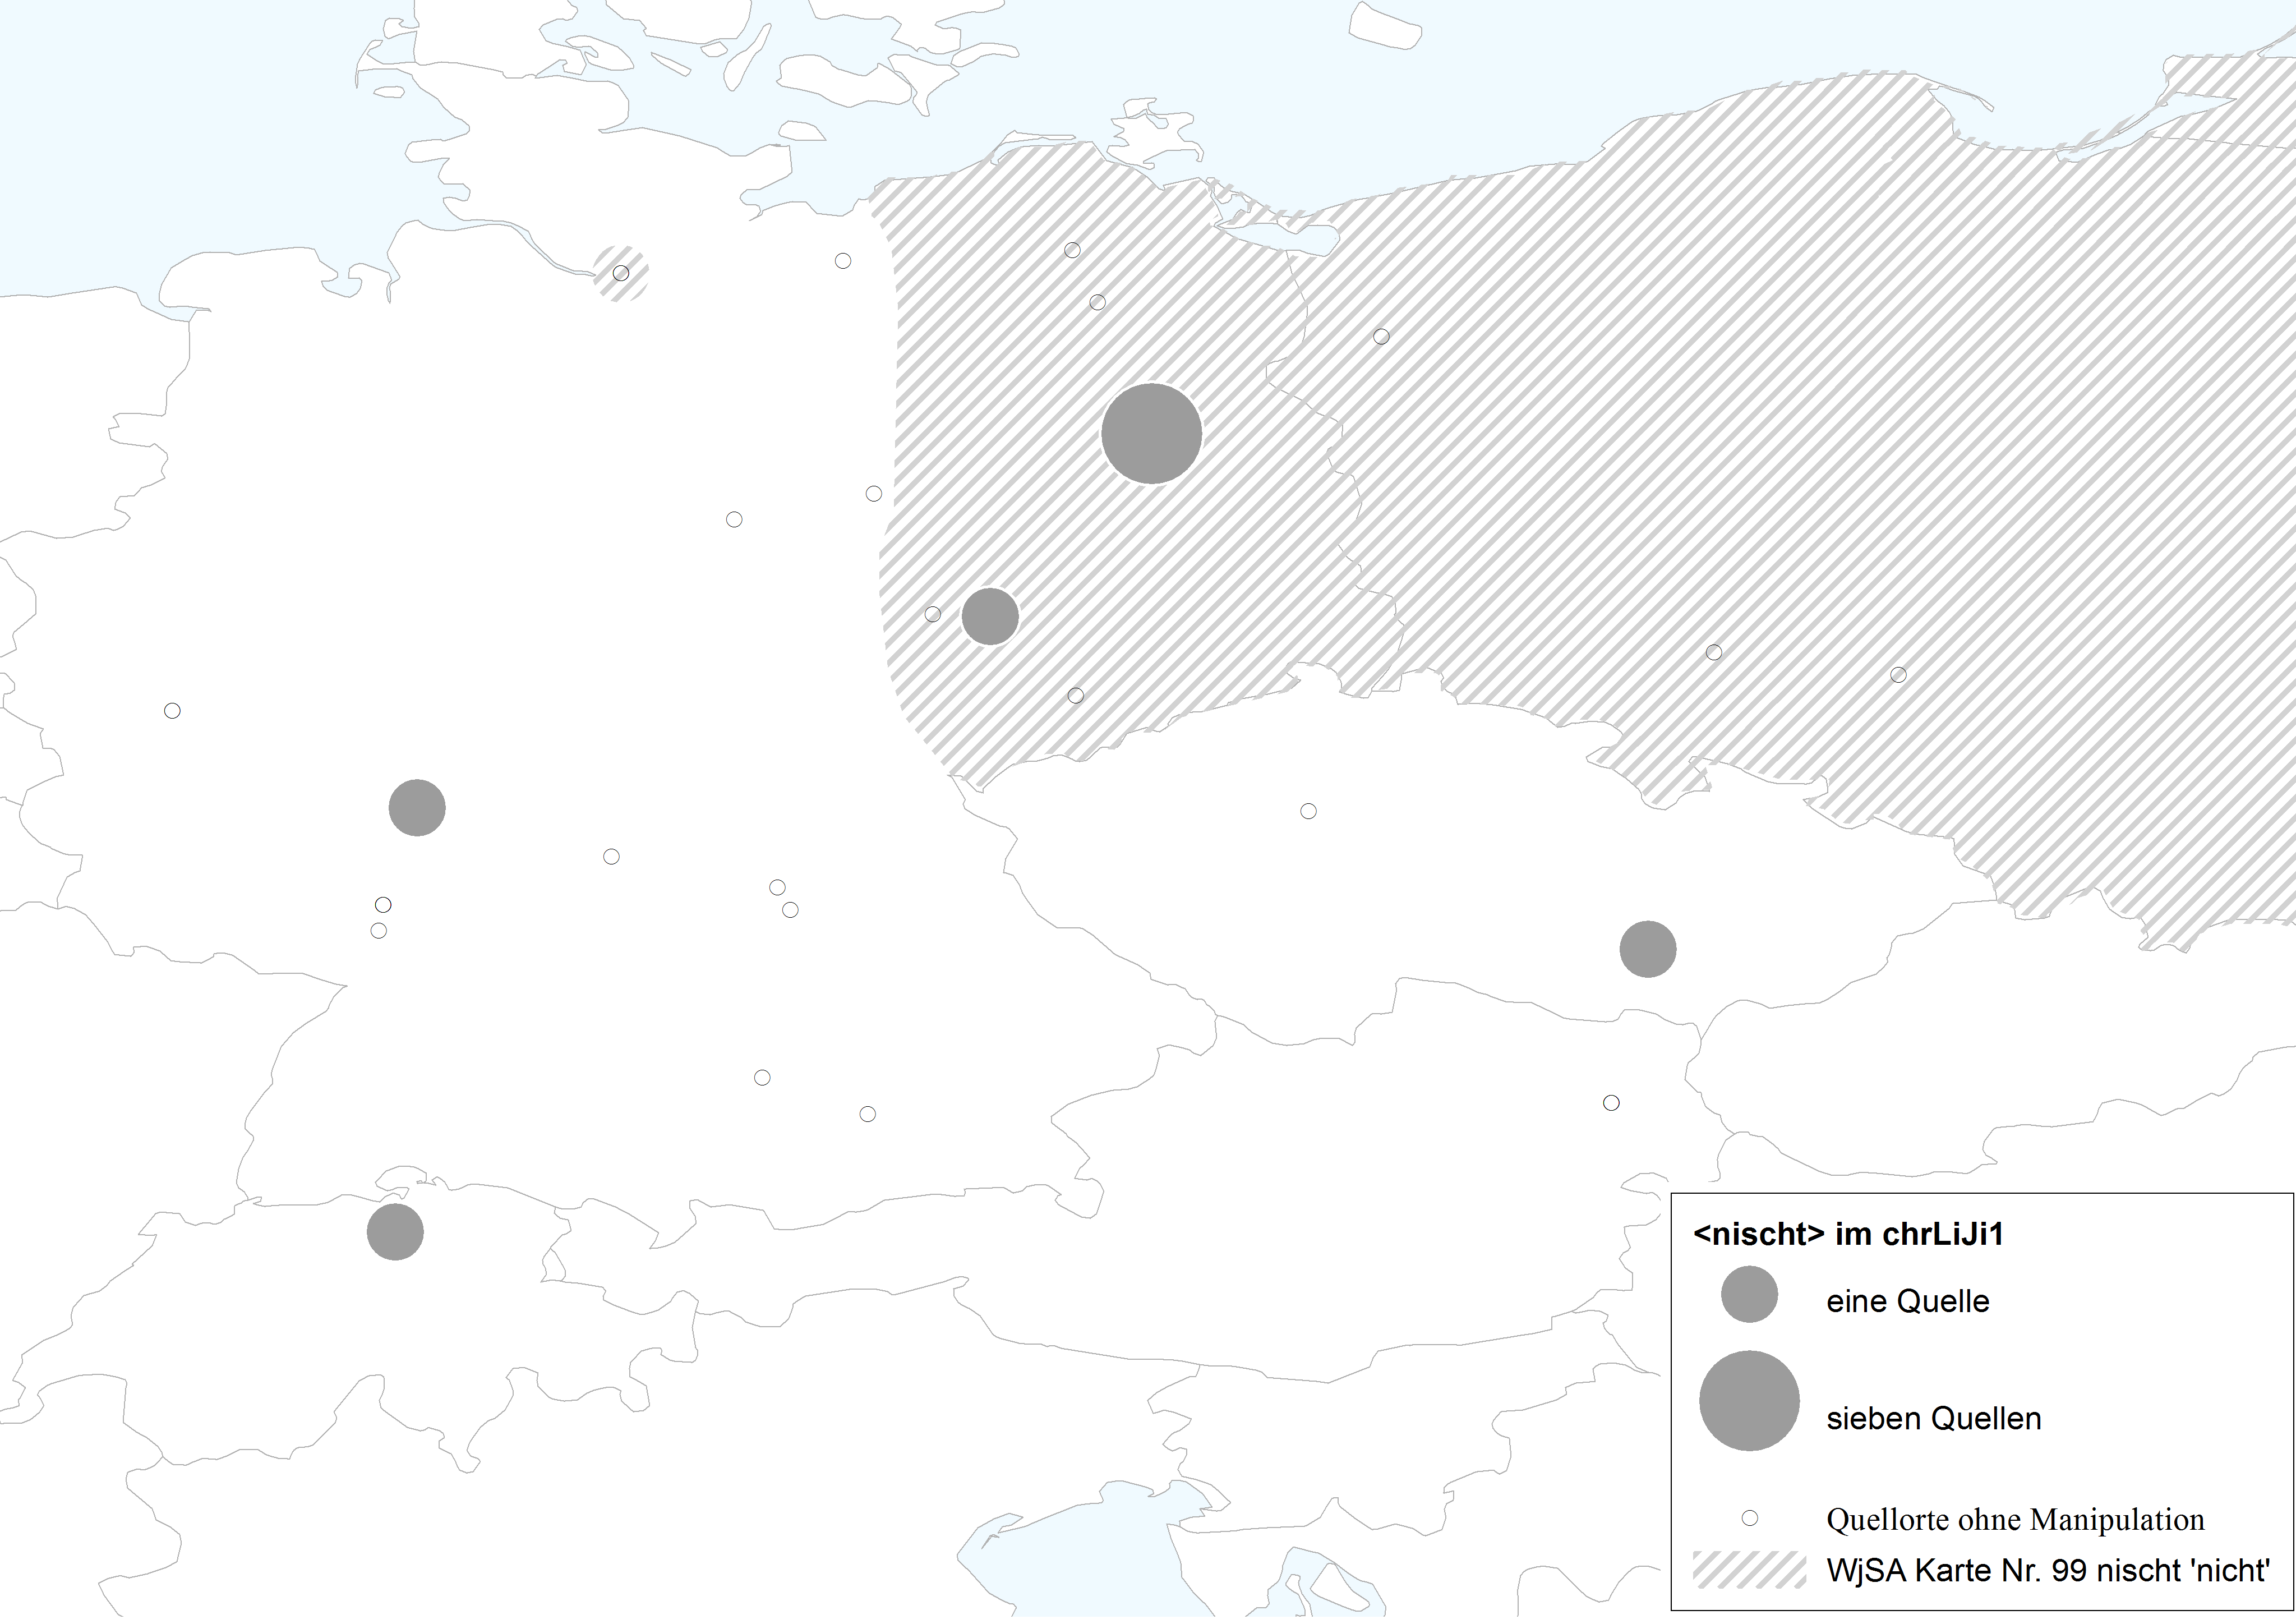
\includegraphics[width=\textwidth]{figures/nischt_karte.png}
		\caption{\label{kartenischt} \textit{nischt} im \hai{chrLiJi1} mit \hai{WjSA} Karte Nr. 99}
		\end{figure}

		
 Im kartographischen Vergleich zum \hai{chrLiJi1} fällt auf, dass insbesondere Quellen aus Berlin und Leipzig die \isi{Koronalisierung} von <ch> im Lexem \sem{nichts} vornehmen. Die Züricher Quelle \hai{AK} (Zürich, 1948), die ebenfalls \textit{nischts} (\isi{Negationspartikel} als auch neg. Indefinitum) setzt, darf als vom \hai{{\OJ}} beeinflusst angesehen werden. Die Frankfurter Quelle \hai{OF} (Frankfurt, 1711), die in den bisherigen Analysen immer sehr nah am \hai{{\WJ}} war, verhält sich mit der \isi{Koronalisierung} besonders untypisch. Hier kann u.\,U. das Frankfurter Rheinfränkisch hineingewirkt haben.


Als ein Beispiel, dass der \hai{WjSA}\footnote{Welcher mit Vorsicht zu genießen ist (vgl.\, \citealt{GuggenheimGruenberg1966b})} in diesem Fall ein glaubwürdiges Bild vermittelt, seien hier zwei authentische westjiddische Quellen zu nennen: Die Autobiographie des Berliners Aron Hirsch Heymann aus den 1880er Jahren (vgl.\, \citealt{Schaefer2013}) und die bereits bekannte hessische Quelle \qu{Die Hochzeit zu Grobsdorf}. Bei Heymann findet man die für das östl. \hai{{\NWJ}} kartierte Form (\ref{bspchhey}), wohingegen die Quelle aus dem westl. \hai{ZWJ}, die von Beranek für diesen Teil des \hai{{\WJ}} übliche Form zeigt  (\ref{bspchgrob}).

 
 \eenumsentence{
\item \textit{nischt(s)} \sem {nicht(s)} (Heymann 1909:\, u.\,a.\, 5, 6, 7, 10, 13) \label{bspchhey}

\item \RL{ניקס} \textit{niks} \sem{nichts} (\qu{Die Hochzeit zu Grobsdorf} 1822:\, u.\,a.\, 4, 6, 10, 11, 12) \label{bspchgrob}
}

  
Sechs der sieben Berliner Quellen des \hai{jüdLiJi1} verwenden, entsprechend der arealen Struktur, \textit{nischt}.\footnote{Die Quellen mit der \isi{Koronalisierung} \textit{nischt} sind: \hai{GuS1}, \hai{GuS5}, \hai{GuS10}, \hai{GuS15}, \hai{GuS23} u. \hai{PBerlin2}.} Die übrigen Texte des \hai{jüdLiJi} manipulieren dieses Lexem nicht.

 
Insgesamt fällt auf, dass die \isi{Koronalisierung} nicht als Regel umgesetzt wird, sondern nur an einem Lexem, wo sie der Form des östl. \hai{{\WJ}} bzw. des \hai{{\OJ}} entspricht. Dieses Phänomen zeigt eine besonders eindeutige areale Verbreitung im \hai{{\LiJieins}}, die den bisher gewonnenen Daten zum \hai{{\WJ}} entspricht.

\section{Deaffrizierung von <z>}\label{sz}
%\noindent
Zehn Quellen des \hai{chrLiJi1} verwenden eine auffällige Graphie der stimmlosen alveolaren Affrikate /ts/ <z> im \isi{Anlaut}, indem sie stattdessen <s> oder <ß> setzen. Besonders betroffen ist das Lexem \sem{zu}, welches als \textit{su} (\hai{AH} Chemnitz, 1789:\,2, 3;\, \hai{BS} Mannheim, 1798:\,4;\, \hai{BW} Leipzig, 1826 Leipzig, 1826:\,99;\, \hai{PF} Augsburg, 1816:\,12, 13;\, \hai{VD} Frankfurt, 1916:\,13, 15, 19) oder als \textit{ßu} (\hai{AJ} Berlin, 1825:\,2, 4, 6;\, \hai{DP} Pyrzyce, 1874:\,15, 19, 29;\, \hai{SV} München, 1890:\, IV, 1, 3, 5, 6, 7;\, \hai{UT} Stavenhagen, 1862:\,Kap.\, 45) auftaucht. Hinter dieser \isi{Orthographie} könnte sich eine \isi{Deaffrizierung} zu einem \isi{Frikativ} verbergen. <ß> kann etwa auf stimmloses [s] verweisen;\, <s> kann sowohl für stimmloses [s] wie auch stimmhaftes [z] stehen. Diese \isi{Deaffrizierung} ist prinzipiell eine im Hochdeutschen mögliche Entwicklung. Analog zu Prozessen im Ostmitteldeutschen, wo die aus der 2. \hai{LV} hervorgegangene Affrikate /pf/ zu /f/ lenisiert wurde, z.\,B.\, [pfʊnt] > md. [fʊnt], kann sich auch /ts/ > /s/, /z/ entwickelt haben (vgl.\, \citealt[273, 282]{Schirmunski1962};\citealt[64f]{Koenig1978};\hai{KDSA} Karten Nr. 21, 22). Im modernen \hai{{\OJ}} fand dieselbe Weiterentwicklung von anlautendem {\germ} \textit{p} > {\mhd} \textit{pf} zu \textit{f} statt (im \isi{Auslaut} > \textit{p}) (\citealt[189]{Kleine2008};\citealt[323–327]{Bin-Nun1973}). Diese wird auch graphematisch umgesetzt, z.\,B.\, \RL{{פ\makebox(-0.8,9)[r]{\libertineGlyph{uni207B}}}ערדל} %format! Diakritikum kontrollieren
\textit{ferdl} \sem{Pferdchen}. Würde es sich bei der Entwicklung /ts/ > /s/, /z/ um eine analoge Ausdehnung \,%rs , streichen
bzw. logische Weiterführung der 2. \hai{LV} handeln, so wäre diese für das Jiddische demnach nicht auszuschließen. Der Karte Nr. 57 des \hai{LCAAJ} zufolge blieb die Affrikate /pf/ im \hai{{\WJ}} allerdings weitgehend erhalten.  Für die jiddischen Varietäten ist allerdings eine \isi{Deaffrizierung} von anlautendem /ts/ nicht bekannt. Und nur im \hai{{\NWJ}} und östl. \hai{ZWJ} findet sich dort die Weiterentwicklung zu /f/. Doch lässt die Setzung von <\RL{{פ\makebox(-0.8,9)[r]{\libertineGlyph{uni207B}}}}> %format!  Diakritikum prüfen
bzw. <\RL{פ}> im westl. \hai{ZWJ} der \qu{Hochzeit zu Grobsdorf} darauf schließen, dass hier der \isi{Frikativ} /f/, bzw. ggf. auch der Plosiv /p/, verwendet wurde;\, zumindest findet sich keine Affrikate verschriftlicht (\ref{bspgrobsdorfpf1})--(\ref{bspgrobsdorfpf2}). Im Gegensatz zur \isi{Deaffrizierung} von /ts/ > /s/, /z/ spielt die von /pf/ > /f/ für das \hai{{\LiJi}} interessanterweise keine Rolle.\footnote{Lediglich in einer Quelle des \hai{jüdLiJi1} finden sich zwei Belege: \textit{Ferd} \sem{Pferde} (\hai{GuS4}:\,5), \textit{Fennig} \sem{Pfennig} (\hai{GuS4}:\,5).} 


 \eenumsentence{

\item \RL{פעננינג} \textit{pennig}, \textit{fennig} \sem{Pfennige} (\qu{Die Hochzeit zu Grobsdorf} 1822:\,38)\label{bspgrobsdorfpf1}

\item \RL{{פ\makebox(-0.8,9)[r]{\libertineGlyph{uni207B}}}ונט}  %format! Diakritikum prüfen
\textit{funt}, \sem{Pfund} (\qu{Die Hochzeit zu Grobsdorf} 1822:\,42, 134)\label{bspgrobsdorfpf2}

}


Eine Setzung von /s/ an der Position von nhd. /ts/ wurde im An- und Inlaut besonders im Lothringischen und Moselfränkischen durchgeführt, ist aber auch im Niederdeutschen zu finden, wo es nach \cite[282]{Schirmunski1962} v.\,a.\, in hochdeutschen Entlehnungen als Hyperkorrektur auftritt. Nach der \hai{KDSA} Karte Nr. 47 findet sich /ts/ > /s/ zumindest im Lexem \textit{zum} auch im Mittelbairischen und vereinzelt im burgenländischen Südmittelbairischen (vgl.\, Abbildung \ref{karteszkdsa}). \cite[282, 273]{Schirmunski1962} vertritt für die mittel- und niederdeutschen Dialekte die Hypothese, dass die Setzung von /s/ bzw. /f/ auf den Einfluss der Standardsprache (\qu{Ausgleichsform}) zurückzuführen ist, da die standarddeutschen Affrikate /ts/ und /pf/ in diesen Dialekten nicht gegeben sind. Sechs Quellen des \hai{chrLiJi1} verwenden <ß> für <z> (im \isi{Anlaut});\, fünf Quellen setzen <s> für <z>. Die Quelle \hai{PF} (Augsburg, 1816) verwendet sowohl die Schreibung <ß> für <z> als auch die von  <s> für <z> und verhält sich somit als einziger Text in diesem Bereich nicht homogen.


\begin{figure}
	\begin{tikzpicture}
		\begin{axis}[only marks, width=0.82\textwidth,height=0.2\textheight,
		legend style={at={(1,1)},xshift=+0.2cm, yshift=-0.44cm,anchor=north west,nodes=left},
			%title={Funktionstypen des sp\"aten Westjiddisch},
			xtick={1700, 1725, 1750, 1775, 1800, 1825, 1850, 1875, 1900, 1925, 1950, 1975}, ytick=\empty,
			x tick label style={/pgf/number format/1000 sep=}, 
			y tick label style={/pgf/number format/1000 sep=},
			%extra y ticks={456.1, 1022.4},
			%extra y tick labels={{456,1},{1022,4}},
			extra y tick style={grid=major,
				tick label style={, ,}},
				ymin=0.7,
				ymax=2.9,
			ylabel={Phänomenbelege},
			enlarge x limits=0.03]	
	
			
\addplot [mark=*, black] table [x=jahr, y=sz_z] {figures/sz_z.txt};%2.3
\addplot [mark=*, gray] table [x=jahr, y=s_z] {figures/s_z.txt};%1.8
\addplot [mark=o, black] table [x=jahr, y=no] {figures/z_no.txt};%1.3


 

			% Andere Formen a={mark=square*,blue},% b={mark=triangle*,red},% c={mark=o,draw=black}}
						\legend{<ß> für <z>, <s> für <z>,unmanipuliert} %macht Legende
		\end{axis}
	\end{tikzpicture}
	\caption{Graphien alveolarer Frikative im \hai{chrLiJi1}}
	\label{histosz}	
\end{figure}




Wie die Karte in Abbildung \ref{kartesz} zeigt, ergibt die Verteilung der Graphien <ß>, <s> für <z> sogar ein areales Raumbild. So wird <ß> vor allem in Quellen des östl. \hai{{\NWJ}} gesetzt, während <s> für <z> im \hai{ZWJ} auftritt.

% \todo{zwischen Grafiken verlorener Satz}

 \begin{figure}
		\centering
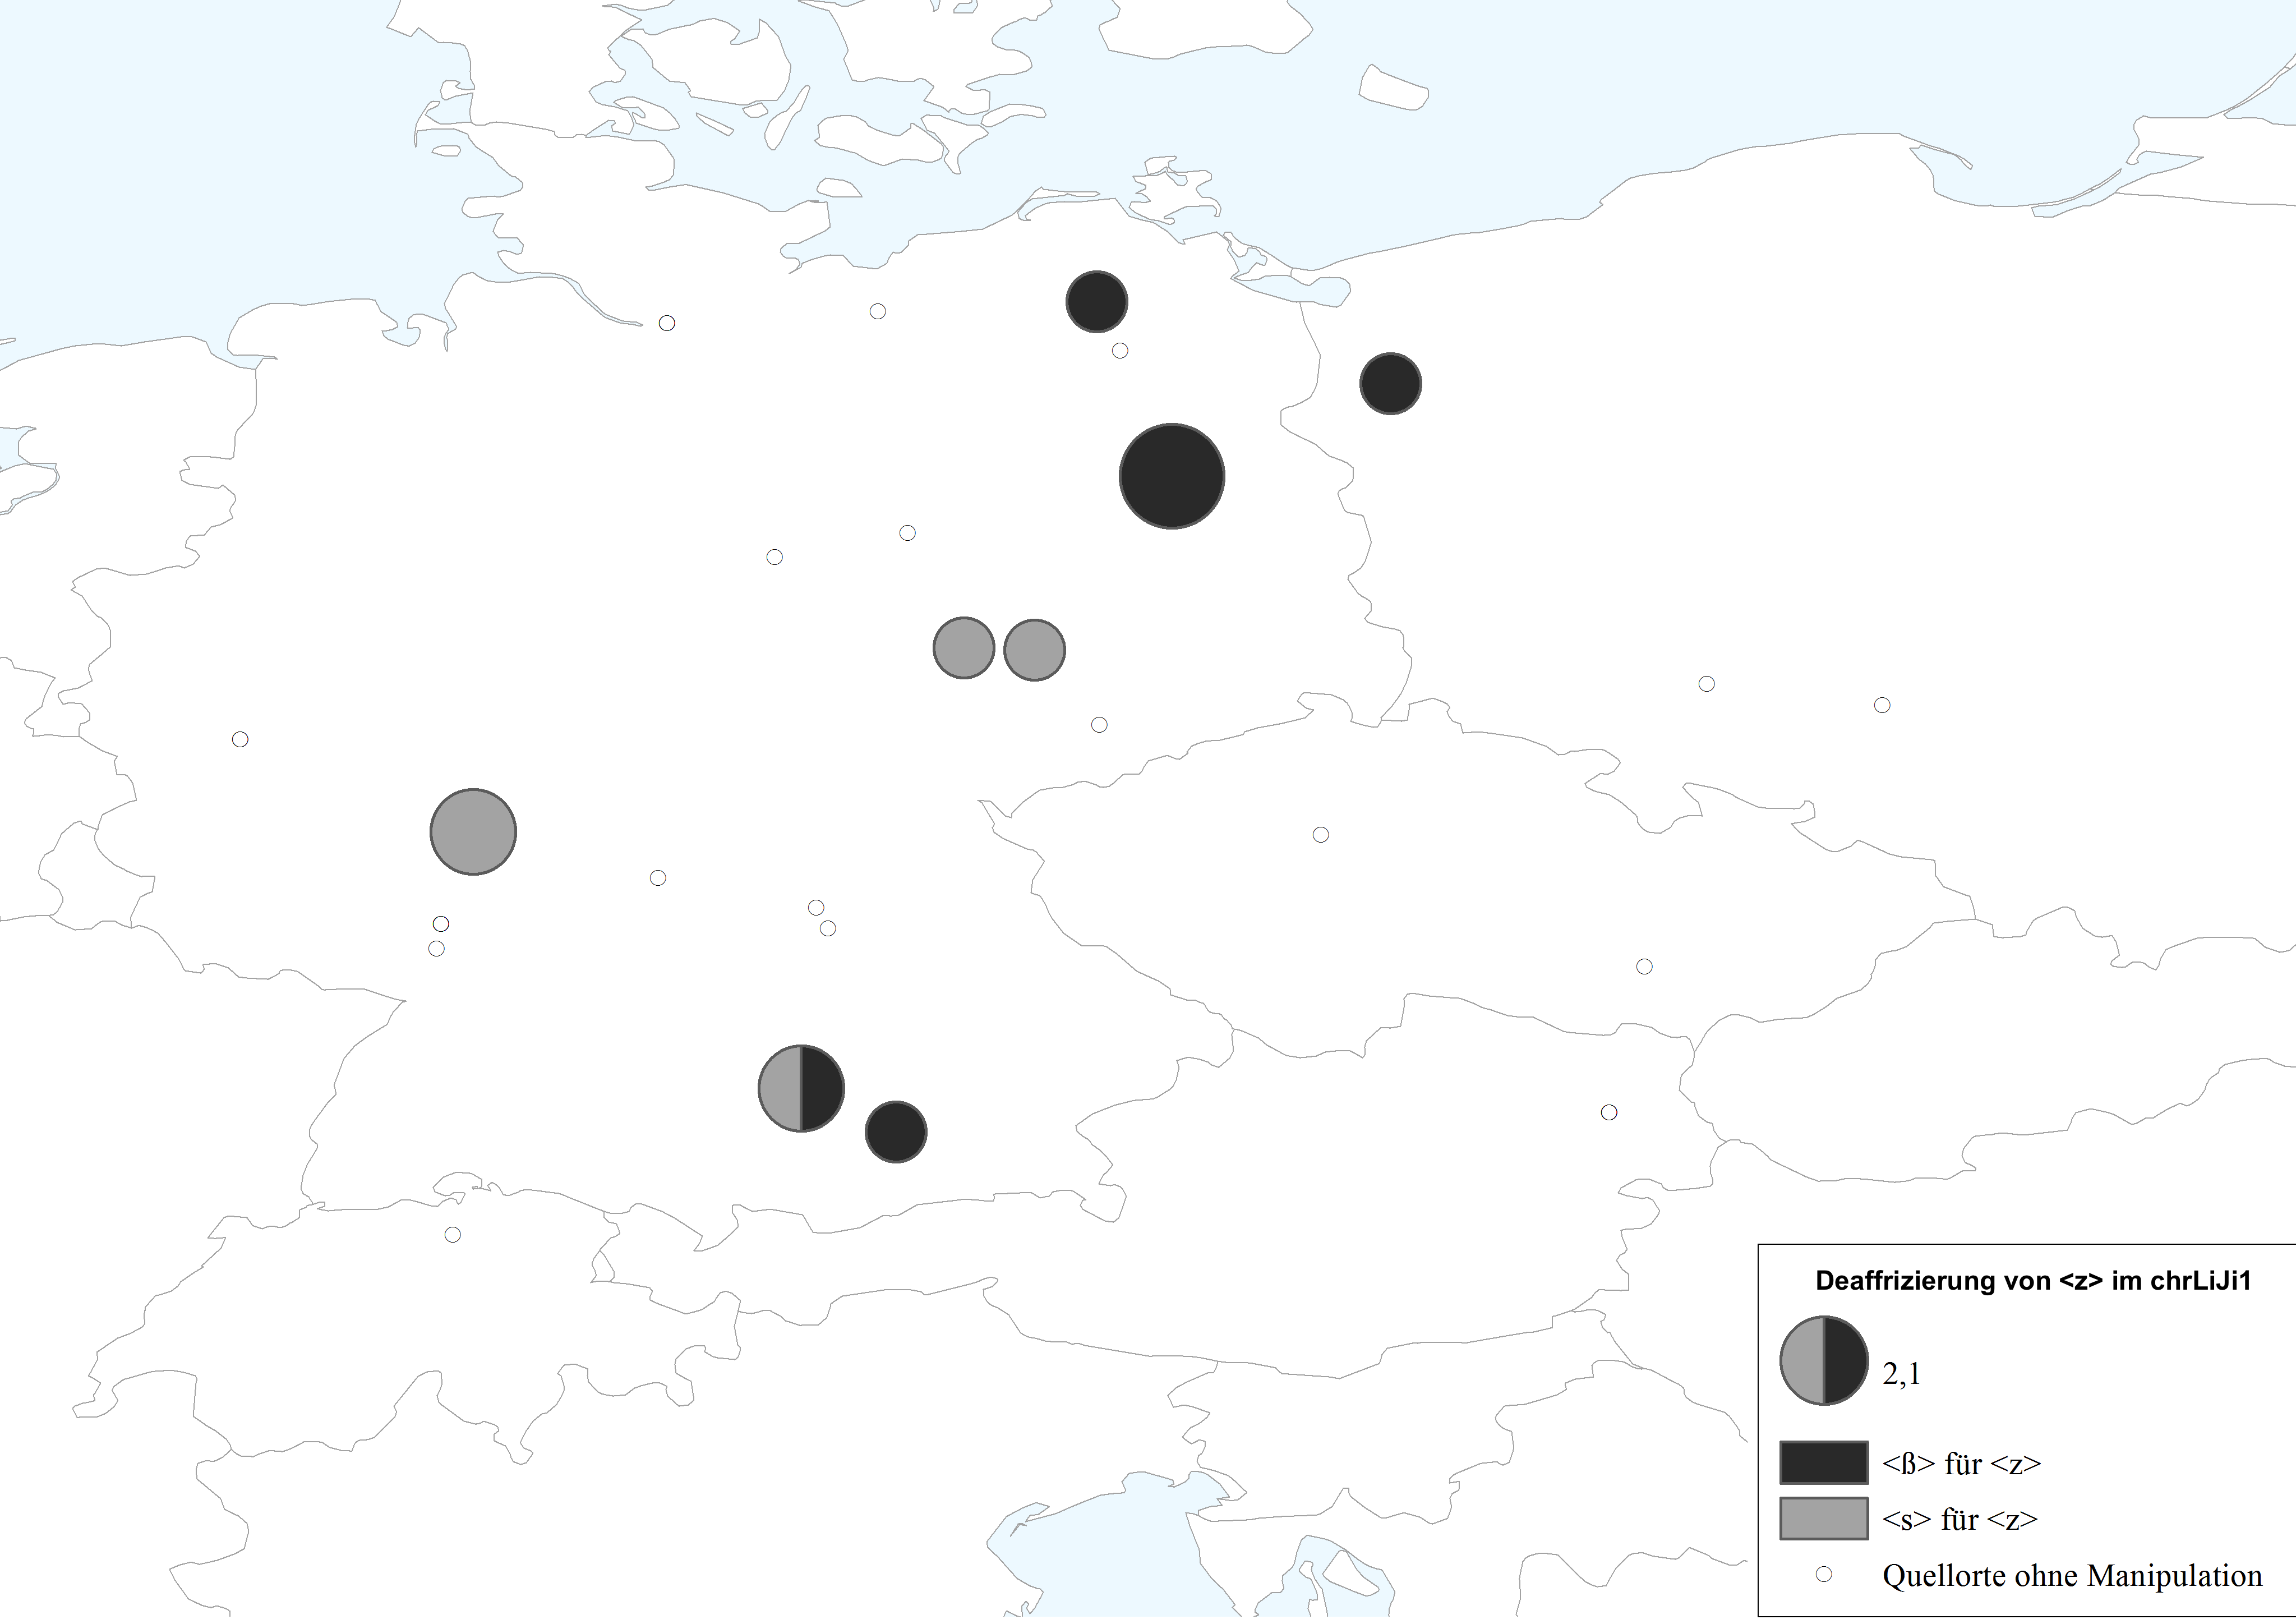
\includegraphics[width=\textwidth]{figures/karte_sz.png}
		\caption{\label{kartesz} <ß>, <s> für <z> im \hai{chrLiJi1}}
		\end{figure}



Dieses Raumbild erstaunt besonders vor dem Hintergrund, dass sich das östl. \hai{{\NWJ}} in Bezug auf Affrikate und Frikative generell anders verhält, als das übrige \hai{{\WJ}}. \cite[1028]{Katz1983} stellt auf Grundlage \,%rs auf Grundlage
von \cite{Friedrich1784}, welcher im \isi{Anlaut} <s> für <z> setzt, fest, dass im \hai{{\NÜJ}}\footnote{Obwohl Friedrich (\citeyear{Friedrich1784}) rein aufgrund der geographischen Verortung links der Oder eher zum \hai{{\NWJ}} zu zählen ist.} die Affrikate /ts/ für anlautendes /s/ gesetzt werde. Der \hai{LCAAJ} (\citeyear[Karten 47, 48, 49]{Herzog1992}) zeigt zumindest, dass durch das westjiddische Sprachgebiet eine Isoglosse verläuft, die auf der Qualität des alveolaren Frikativs als stimmhaft [z] bzw. stimmlos [s] beruht (vgl.\, Abb \ref{karteszlcaaj}).\footnote{In den Karten des \hai{LCAAJ} entspricht <z> der im englischen Sprachraum üblichen Notation für den stimmhaften \isi{Frikativ} [z].} 
Doch eine Markierung dieses Phänomens ($\pm$ stimmhaft) wird im \hai{{\LiJi}} nicht verschriftlicht. Stattdessen wird mit der \isi{Deaffrizierung} von /ts/ <z> > /s/ <s>, <ß>, /z/ <s> eine gegensätzliche Entwicklung gezeigt. Das Areal der \isi{Deaffrizierung} im \hai{chrLiJi1} trifft jedoch auch relativ gut mit der Fortisierung im östl.\,\hai{{\NWJ}} zusammen (s. Abbildung \ref{karteszlcaaj}). Eine wenig plausible Erklärung für die Vermeidung des <z>-Graphems im \hai{chrLiJi1} könnte demnach sein, dass dort eigentlich die Fortisierung umgesetzt werden sollte, stattdessen aber eine \isi{Deaffrizierung} graphematisiert wurde. Diese Hypothese kann jedoch nicht erklären, wieso <s> für <z> im zentralwestjiddischen Gebiet des \hai{chrLiJi1} gesetzt wird. Plausibler scheint es, diese Graphien als Ausdruck einer \isi{Deaffrizierung} zu interpretieren, von deren Existenz im \hai{{\WJ}} bislang jedoch nichts bekannt ist.

 \begin{figure}[t]
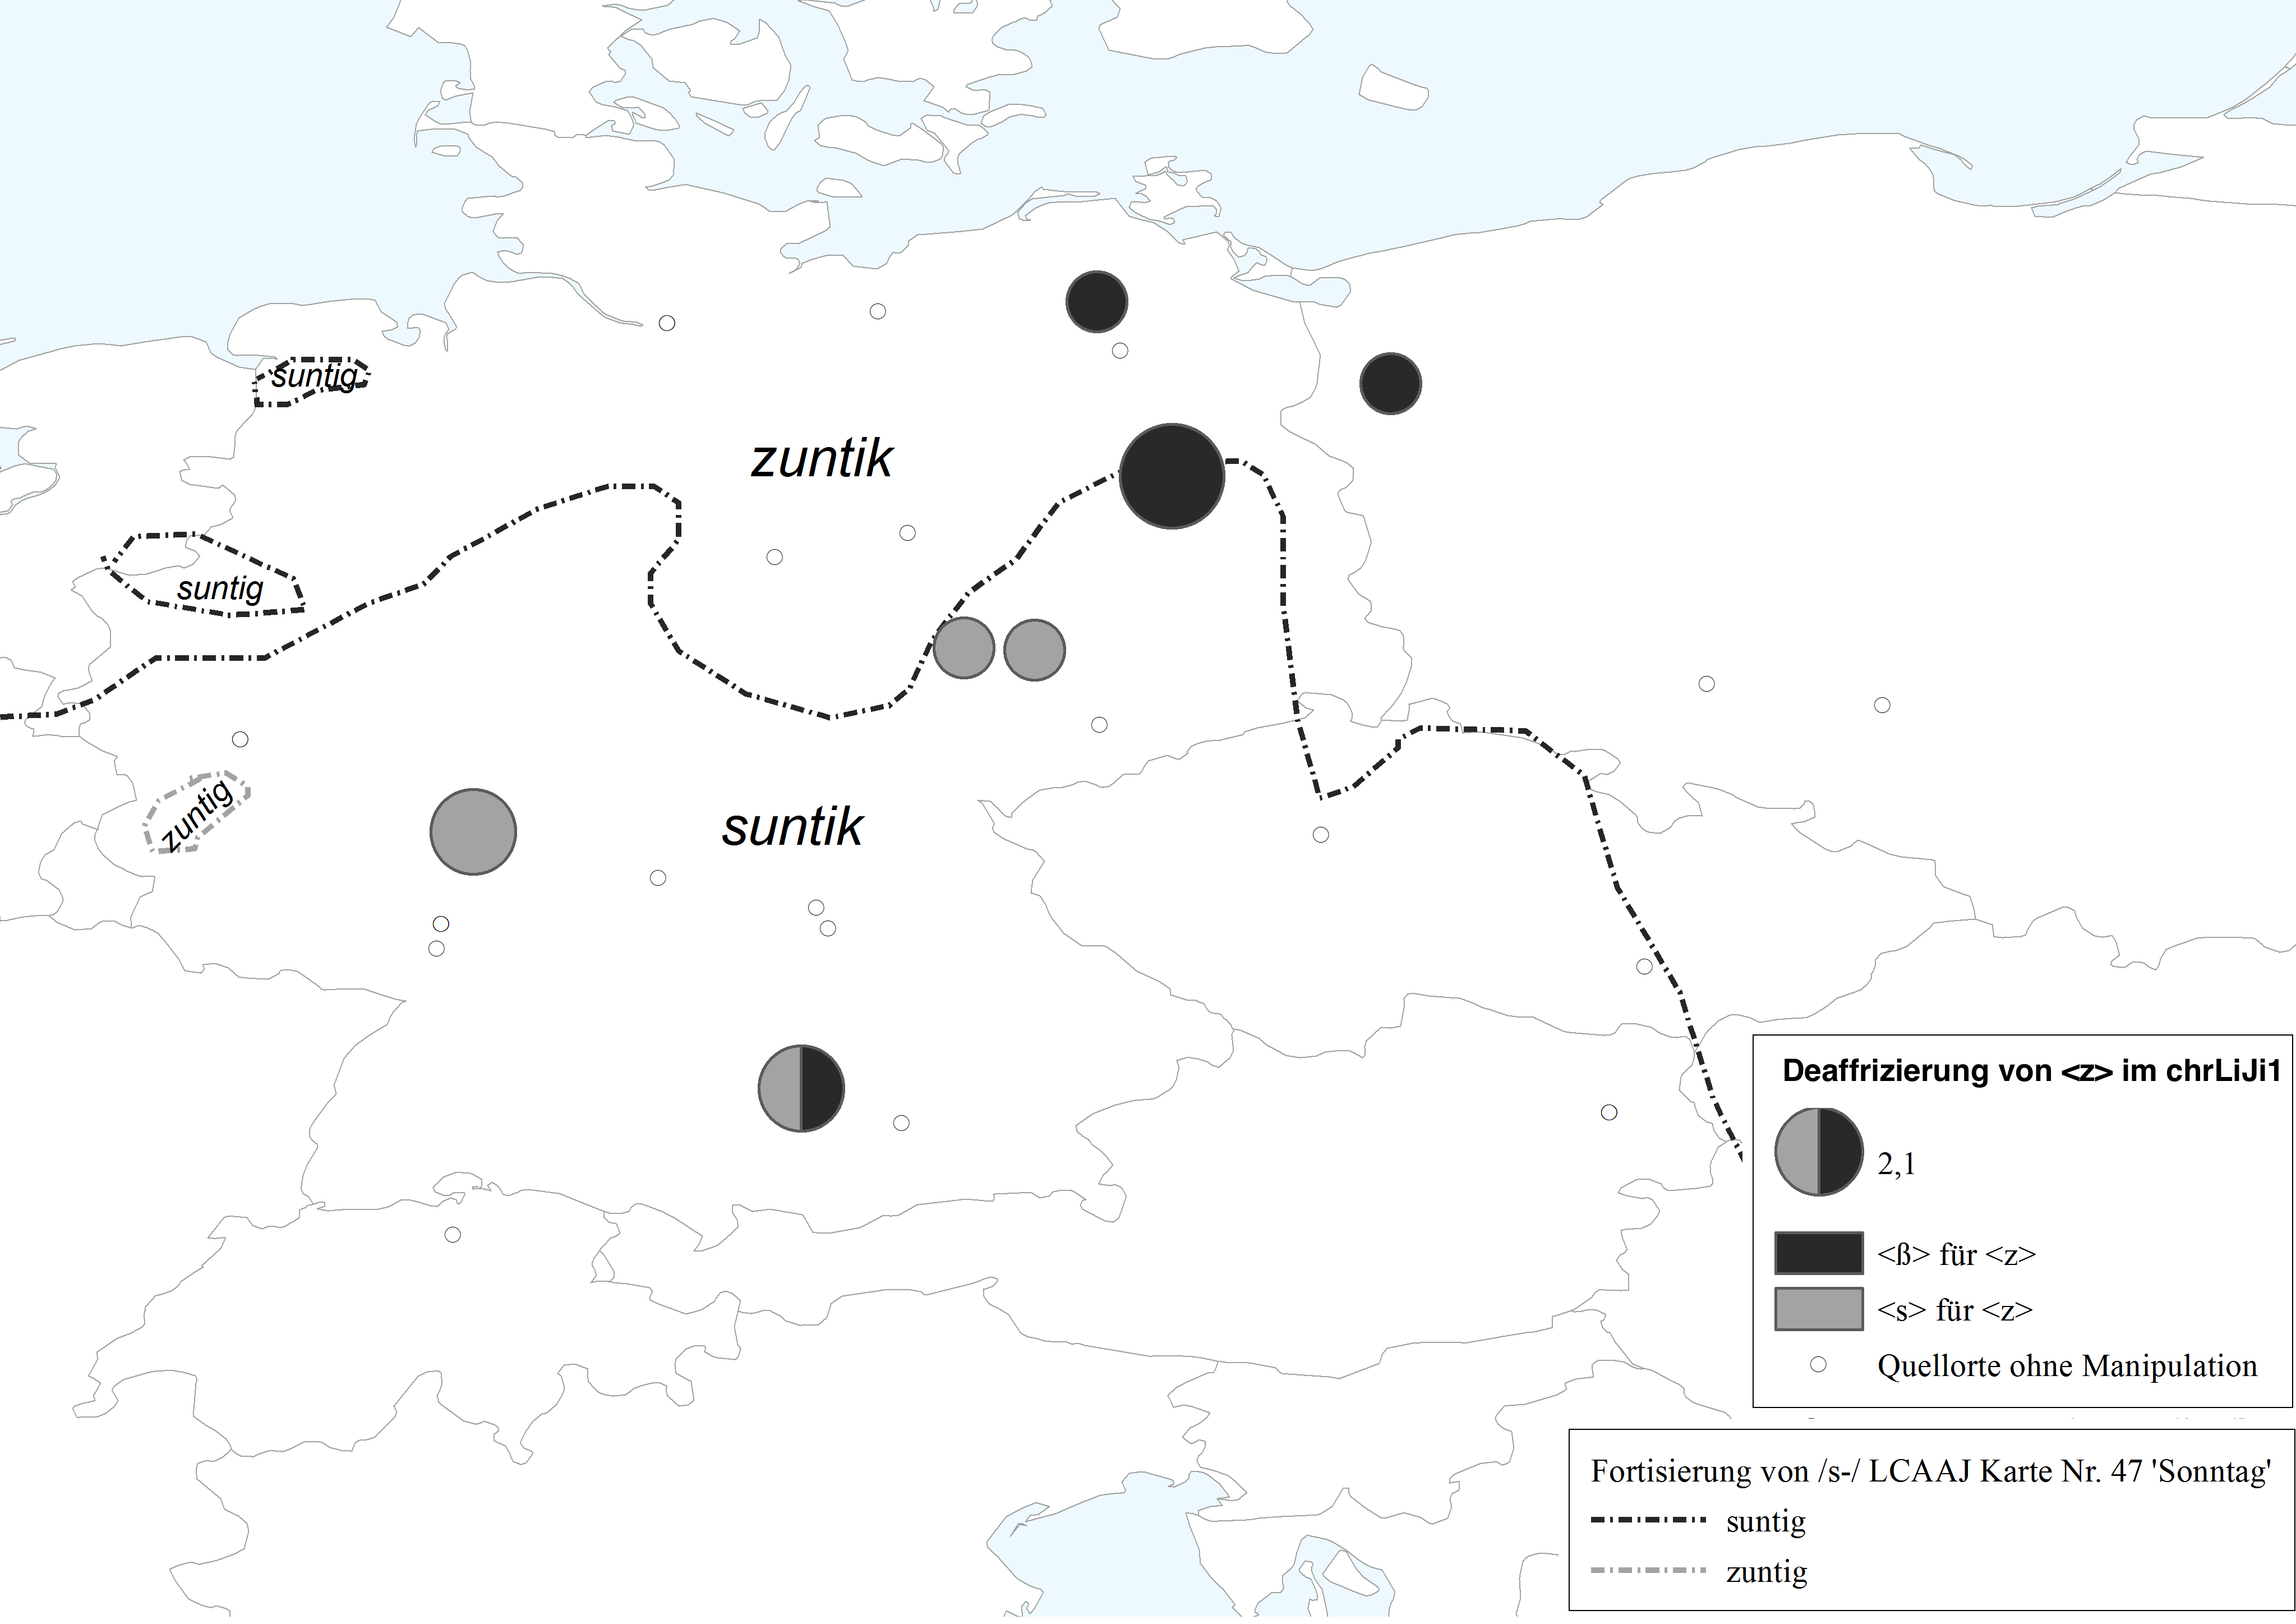
\includegraphics[width=\textwidth]{figures/karte_sz_lcaaj.png}
		\caption{\label{karteszlcaaj} <ß>, <s> für <z> im \hai{chrLiJi1} mit \hai{LCAAJ} Karte Nr. 47}
		\end{figure}


 
Die Belege von <s> für <z> in vier Quellen im Obersächsischen und Frankfurter Rheinfränkischen lassen sich auf Interferenzen aus den deutschen Dialekten zurückführen. 
Wie die Karte in Abbildung \ref{karteszkdsa} zeigt, ist genau in diesen Regionen die 2. \hai{LV} an anlautendem {\germ} \textit{t} weitergeführt worden zu /\textit{s}/. Es ist nicht auszuschließen, dass möglicherweise auch die örtlichen westjiddischen Varietäten an dieser Entwicklung teilgenommen haben. Allerdings fehlen bislang vergleichbare authentische Daten zum \hai{{\WJ}} aus diesen Regionen, die dies bestätigen bzw. widerlegen. Auch die Belege für <ß> statt <z> im Nordosten können auf einer entsprechende Entwicklung von /ts/ > /s/ im Niederdeutschen beruhen (vgl.\, \citealt[282]{Schirmunski1962}). Offen bleibt hierbei allerdings, warum das Graphem <ß> gewählt wurde und andernorts <s>. Gegebenenfalls wollten die Autoren mit der Setzung von <ß> die Stimmlosigkeit des Frikativs stärker hervorheben.


 \begin{figure}
		\centering
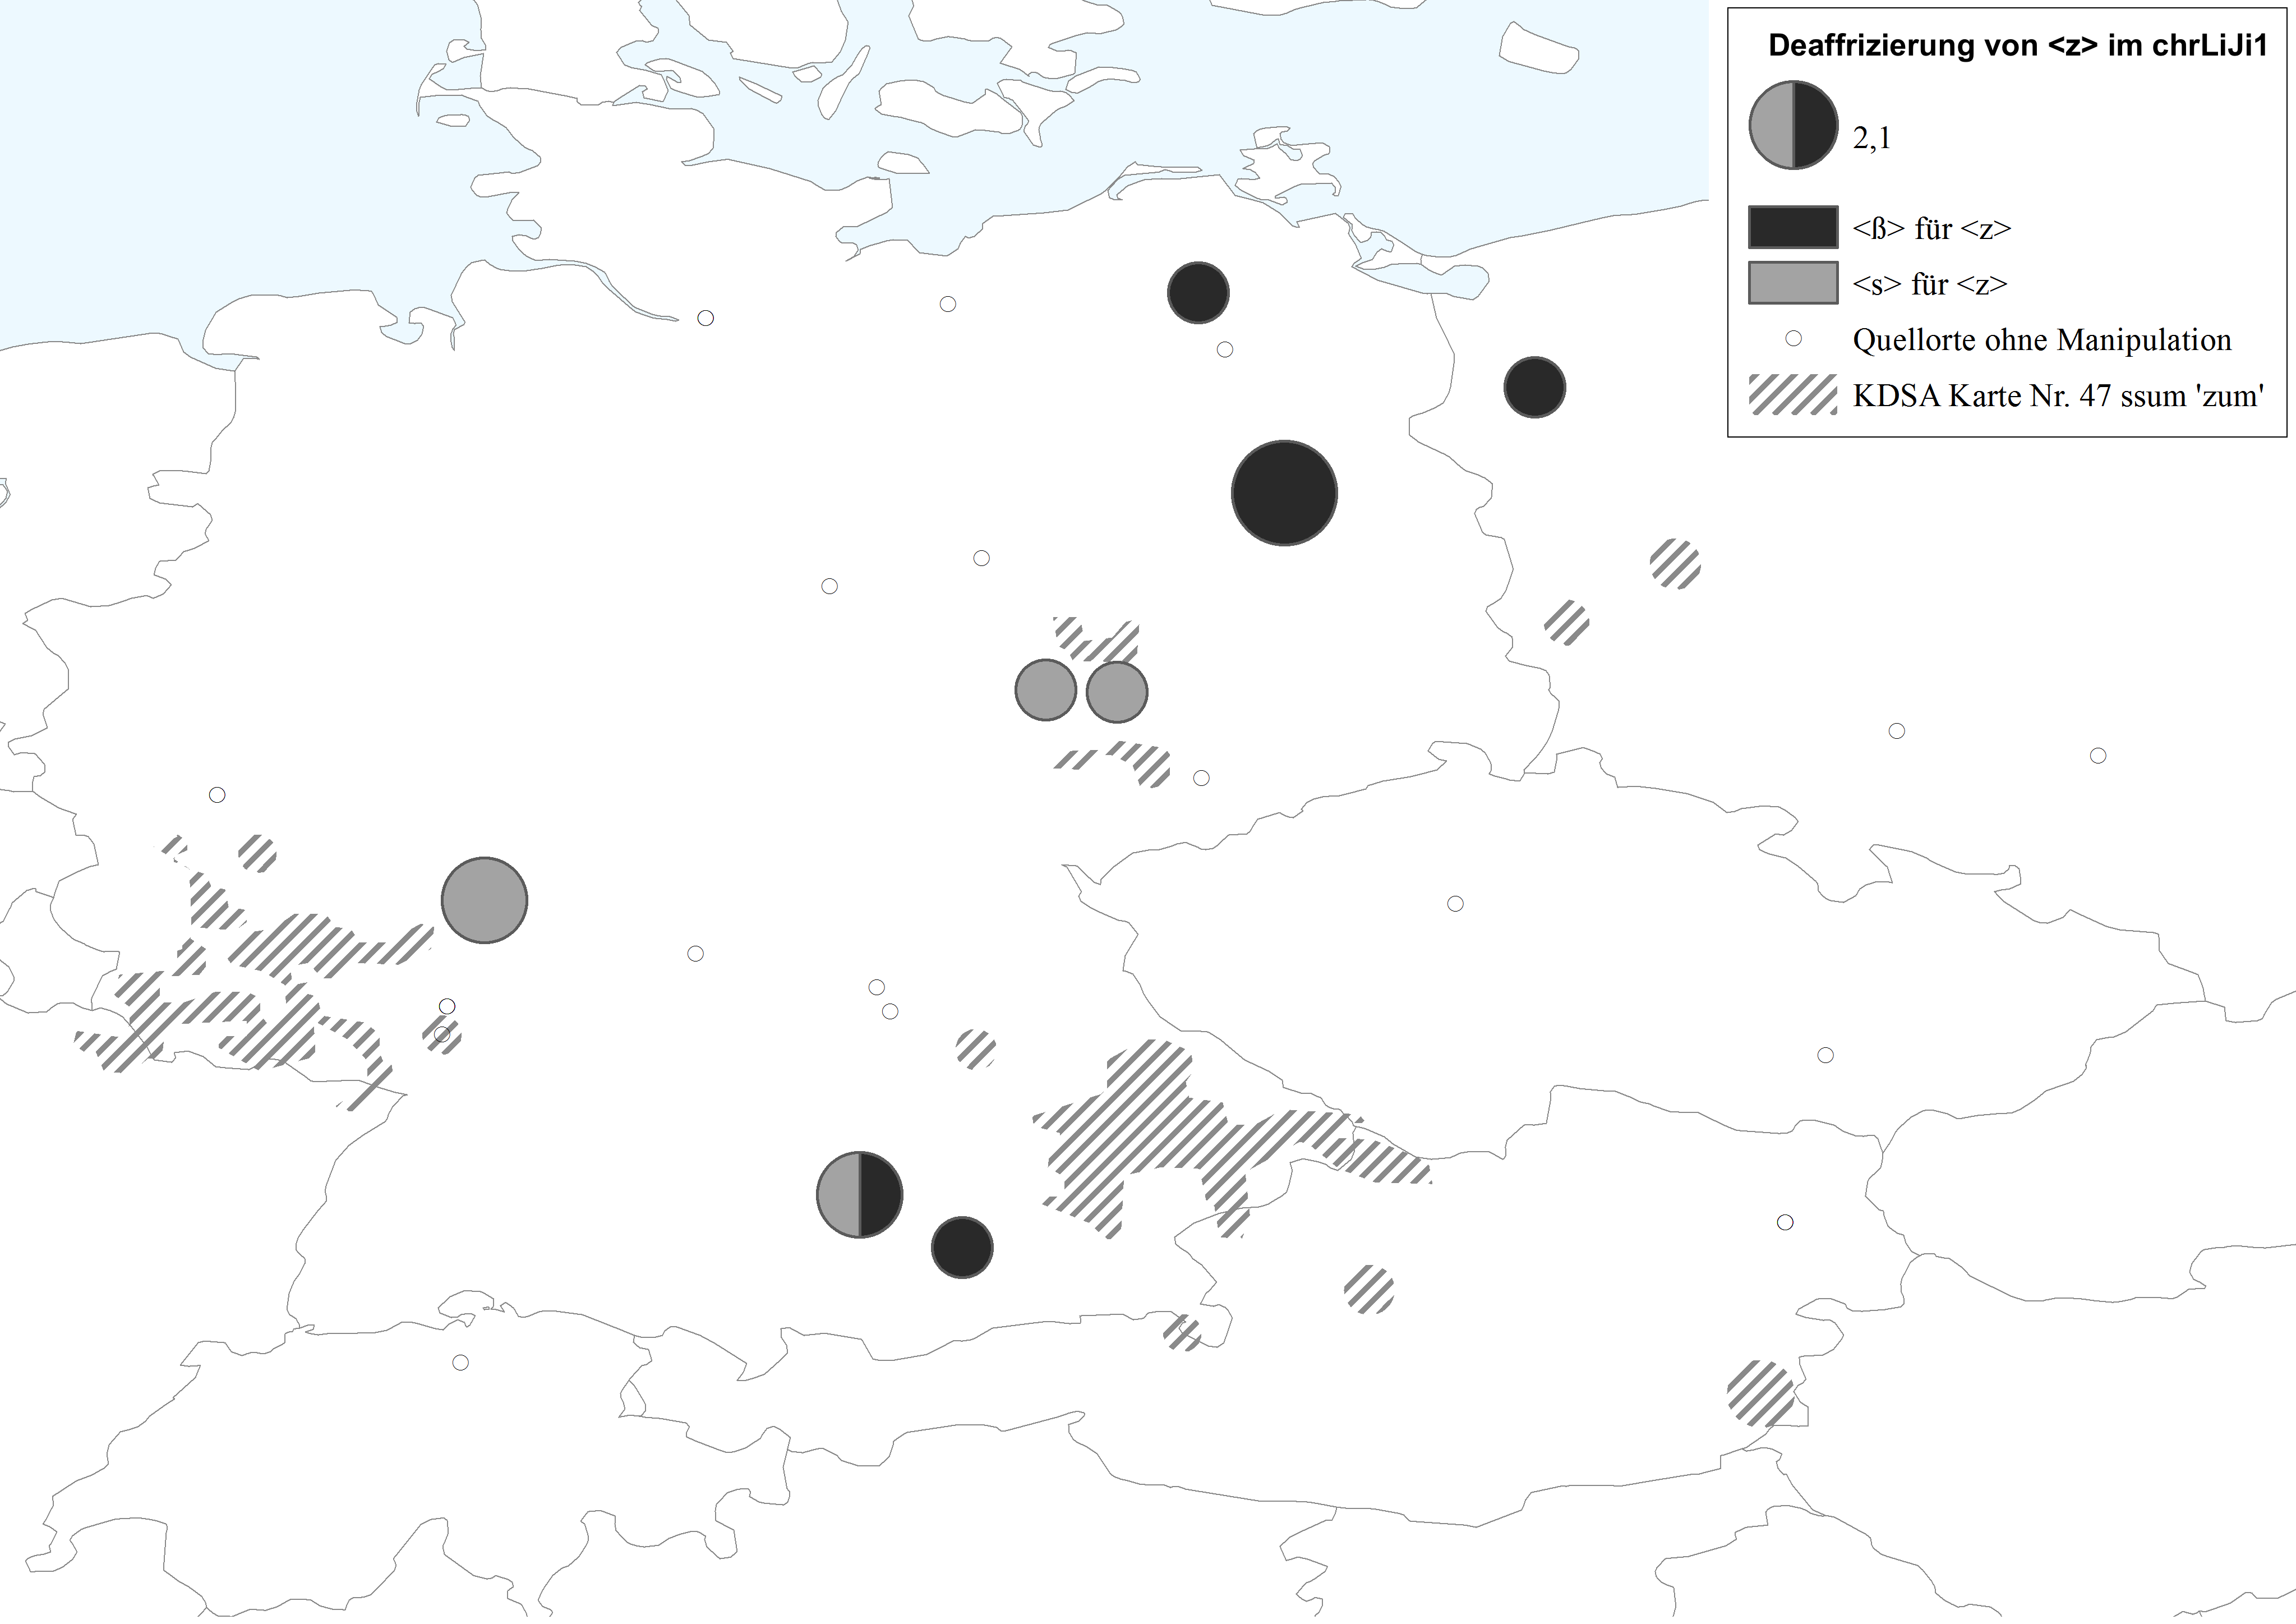
\includegraphics[width=\textwidth]{figures/karte_sz_kdsa2.png}
		\caption{\label{karteszkdsa} <ß>, <s> für <z> im \hai{chrLiJi1} mit \hai{KDSA} Karte Nr. 47}
		\end{figure}


  
<ß>-Graphien für <z> finden sich auch im \hai{jüdLiJi1} in drei Berliner Quellen und dem Pamphlet aus Alsleben.\footnote{Im Einzelnen sind diese Quellen: \hai{GuS10}, \hai{GuS23}, \hai{PAlsleben}, \hai{PBerlin2}.} Das verweist zumindest darauf, dass die Formen im \hai{chrLiJi1} unter Umständen auf eine im östlichen \ili{Westjiddisch} tatsächlich gegebene Sprachrealität verweisen. Die Schreibung <s> für <z> findet sich im \hai{jüdLiJi1} nicht.


  \section{Plosive}\label{plosivekap} 
  Im Bereich der \isi{Plosive} lassen sich im \hai{{\LiJi}} anhand der Graphie Fortisierungen und Lenisierungen erkennen. Insbesondere sind hier Wechsel zwischen Mediæ und Tenues zu finden. Diese werden in den folgenden Unterabschnitten einzeln dargestellt. Wie die Tabelle \ref{tblphonall} (S.\, \pageref{tblphonall}) zeigt, treten diese Manipulationen im \hai{{\LiJi}} eher selten auf. In den wenigen Fällen ist es jedoch von besonderem Interesse zu untersuchen, ob der örtliche deutsche Dialekt die Imitationen beeinflusste oder ob es andere Erklärungen dafür gibt, warum \isi{Plosive} nur in bestimmten Quellen manipuliert wurden.
  
19 Quellen des \hai{chrLiJi1} zeigen Manipulationen der Graphien von Plosiven. Wie das Histogramm in Abbildung \ref{diagrammplosive} zeigt, streuen die Belege über den gesamten Untersuchungszeitraum hinweg. Die meisten Quellen, die diese Manipulationen einsetzen, finden sich jedoch in den 100 Jahren zwischen 1770 und 1870.   
   

\begin{figure}
	\begin{tikzpicture}
		\begin{axis}[only marks, width=0.82\textwidth,height=0.2\textheight,
		legend style={at={(1,1)},xshift=+0.2cm, yshift=-0cm,anchor=north west,nodes=left},
			xtick={1700, 1725, 1750, 1775, 1800, 1825, 1850, 1875, 1900, 1925, 1950, 1975}, ytick=\empty,
			x tick label style={/pgf/number format/1000 sep=}, 
			y tick label style={/pgf/number format/1000 sep=},
			extra y tick style={grid=major,
				tick label style={, ,}},
				ymin=0.7,
				ymax=2.7,
			ylabel={Phänomenbelege},
			enlarge x limits=0.03]	
	
			
\addplot [mark=*, gray] table [x=jahr, y=dt] {figures/dt.txt};%2.4
\addplot [mark=*, black] table [x=jahr, y=bp] {figures/bp.txt};%2.1
\addplot [mark=square*,black] table [x=jahr, y=pb] {figures/pb.txt};%1.7
\addplot [mark=square*, gray]  table [x=jahr, y=kg] {figures/kg.txt};%1.3
\addplot [mark=o, black] table [x=jahr, y=no] {figures/plosive_no.txt};%0.9


						\legend{<d> statt <t>, <b> statt <p>, <p> statt <b>, <k> statt <g>,  unmanipuliert} %macht Legende
		\end{axis}
	\end{tikzpicture}
	\caption{Orthographische Manipulationen von Plosiven im \hai{chrLiJi1}}
	\label{diagrammplosive}	
\end{figure}

   
  
 \subsection{Lenisierung <d> statt <t>}\label{td}
   %  %\noindent
In acht Quellen des \hai{chrLiJi1} tritt die Schreibung <d> statt <t> auf. In fünf Quellen findet diese \isi{Lenisierung} im \isi{Anlaut} statt (\ref{bspdt1}–\ref{bspdt5}) und in ebenfalls fünf Texten im Inlaut (\ref{bspdt6}–\ref{bspdt10}). Die Aufhebung des Fortis-Lenis-Kontrast ist der Karte Nr. 50 des \hai{LCAAJ} (\citeyear[99]{Herzog1992}) zufolge in den südwestjiddischen und westlichen zentralwestjiddischen Varietäten durchgeführt worden.\footnote{Diese mögliche Eigenheit des \hai{{\SWJ}} und \hai{ZWJ} findet sich auch in Heymanns Autobiographie aus Berlin. Auf den Seiten 167 u. 375 arbeitet er bei der Figurenrede von Personen aus Nürnberg und Mainz besonders stark mit der Aufhebung des Fortis-Lenis-Kontrasts (vgl.\, \citealt[33f]{Schaefer2010}).} Allerdings erfolgt die Aufhebung des Kontrasts in diesen Teilen des \hai{{\WJ}} zugunsten der Fortis und nicht, wie in den meisten Quellen des \hai{chrLiJi1} zugunsten der Lenis. Die Stärkung der Fortis ist für die deutschen Dialekte eher selten und lediglich für kleine Teile des Ostfränkischen belegt (\hai{KDSA} Karte Nr. 50;\, \citealt[63]{Fink1930}). Die Fortisierung tritt im \hai{chrLiJi1} einmalig in der Züricher Quelle \hai{AK} (Zürich, 1948) im \isi{Anlaut} auf (\ref{bsptdak}).
 

 \eenumsentence{
 
 \item \textit{Doler} \sem{Taler} (\hai{AD} Leipzig, 1846:\,130) \label{bspdt1}
  \item  \textit{Daeubchen} \sem{Täubchen} (\hai{PG} Speyer, 1835:\,11) \label{bspdt2}
 \item \textit{duhn} \sem{tun} (\hai{TH} Merseburg, 1820:\,98, 135), \textit{Dautropfen} \sem{Tautropfen} (\hai{TH} Merseburg, 1820:\,135) \label{bspdt3}
 \item \textit{daugt} \sem{taugt} (\hai{UT} Stavenhagen, 1862:\,Kap.\, 3) \label{bspdt4}
 \item \textit{det} \sem{tät} (\hai{VD} Frankfurt, 1916:\,15, 16, 19),\, \textit{Dag} \sem{Tag}\, (\hai{VD} Frankfurt, 1916:\,19)\label{bspdt5}
  \item  \textit{unden} \sem{unten} (\hai{DW} Wien, 1773:\,111) \label{bspdt6}
 \item \textit{geknädet} \sem{geknetet} (\hai{OF}:\,1) \label{bspdt7}
 \item \textit{uffgedahn} \sem{aufgetan} (\hai{PG} Speyer, 1835:\,8) \label{bspdt8}
 \item \textit{Hindern} \sem{Hintern} (\hai{PL} Mannheim, 1780:\,49) \label{bspdt9}
 \item \textit{Vader} \sem{Vater} (\hai{VD} Frankfurt, 1916:\,15R),  \textit{gedahn} \sem{getan} (\hai{VD} Frankfurt, 1916:\,21R) \label{bspdt10}
 
 
 \item \textit{tunkel} \sem{dunkel} (\hai{AK} Zürich, 1948:\,247) \label{bsptdak}
 } 
 
 Die \isi{Lenisierung} von /t/ > /d/ hingegen ist in den deutschen Dialekten weit verbreitet (vgl.\, Abbildung \ref{kartedtkdsa}). Für die jiddischen Varietäten liegen keine vergleichbaren Daten vor;\, keine der authentischen \hai{A1}-Quellen des Westjiddischsamples weist  diese Entwicklung vor. Wie die areale Verbreitung dieses Phänomen im \hai{chrLiJi1} zeigt, ist anzunehmen, dass diese Formen auf Interferenzen mit den deutschen Varietäten beruhen, da alle relevanten Quellen im Lenisierungsgebiet der deutschen Mundarten liegen. Es kann jedoch nicht ausgeschlossen werden, dass diese \isi{Lenisierung} nicht tatsächlich in den späten westjiddischen Dialekten aufgrund des Sprachkontakts zu den deutschen Dialekten erfolgte. Möglicherweise wurde mit dieser Manipulation lediglich versucht, den Aspekt der Dialektalität jüdischer Figuren herauszuarbeiten. Dafür spricht auch, dass die Setzung von <d> für <t> in keiner Quelle des \hai{jüdLiJi1} zu finden ist. %Ebenso fehlt sie im \hai{LiJi2}.
 
 
  \begin{figure}
		\centering
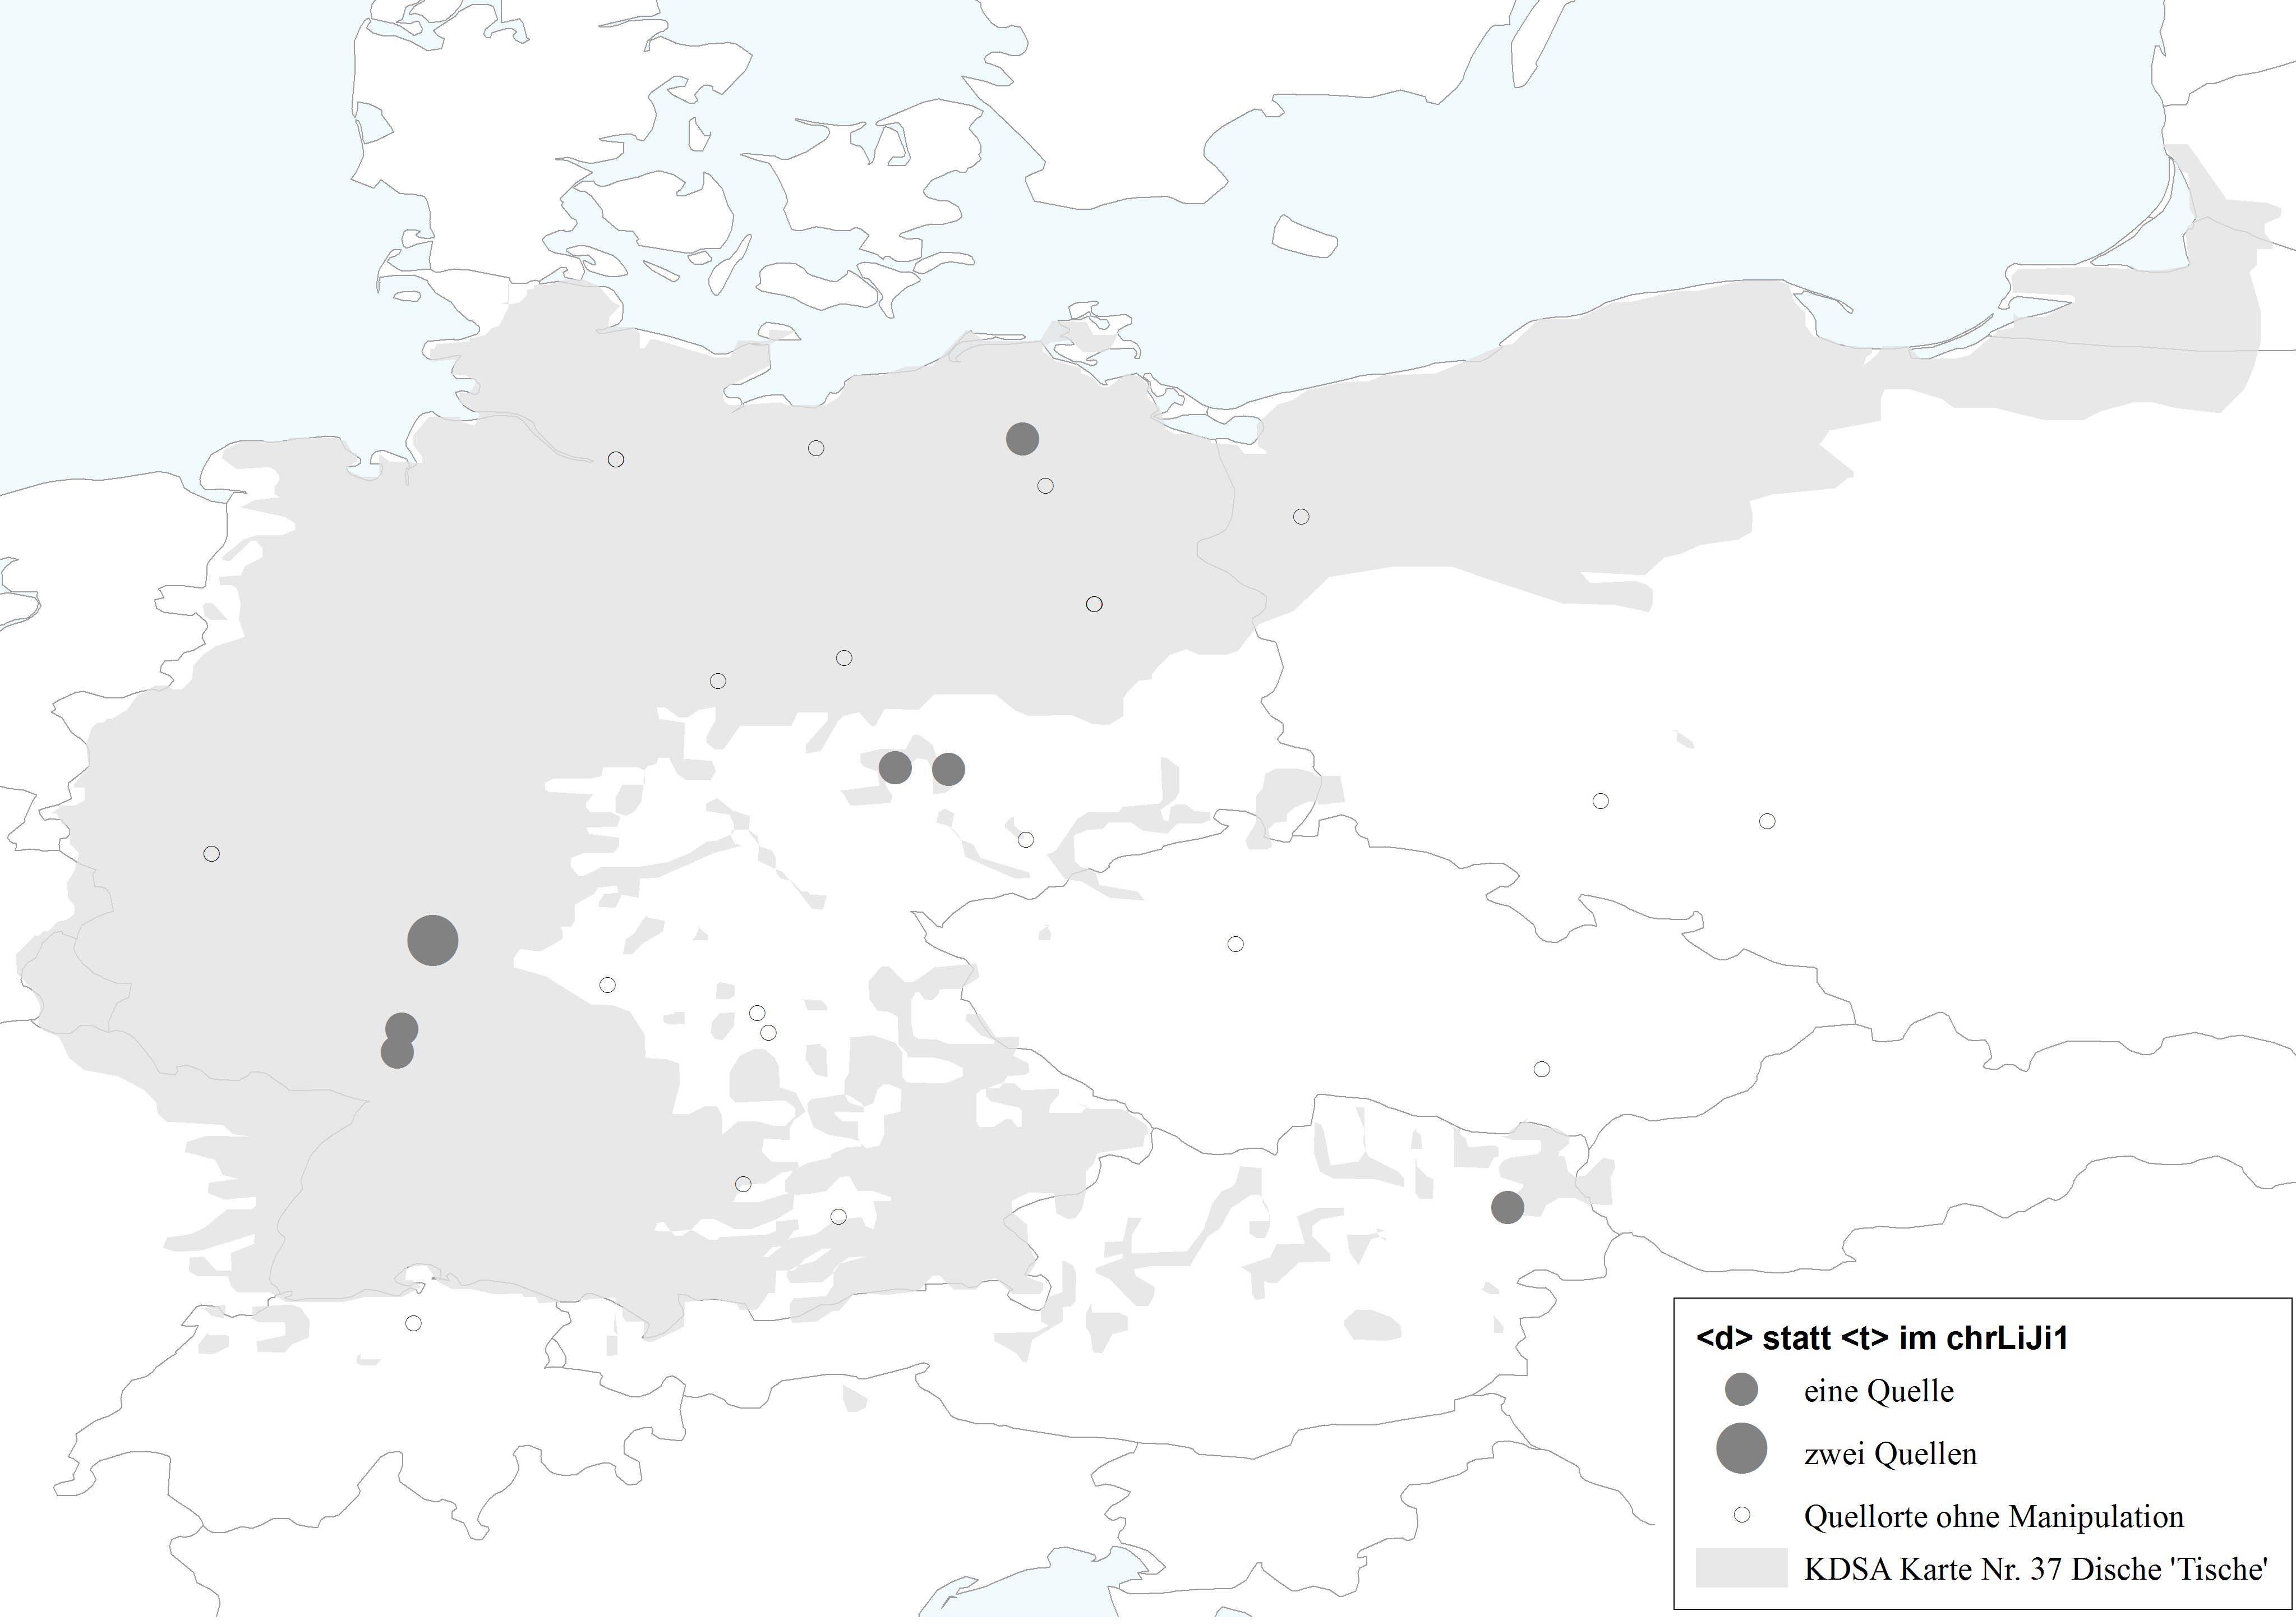
\includegraphics[width=\textwidth]{figures/karte_dt_KDSA37.png}
		\caption{\label{kartedtkdsa} \isi{Lenisierung} von <d> im \hai{chrLiJi1} und den mod. dt. Dialekten (\hai{KDSA} Karte Nr. 37)}
		\end{figure}





  
  \subsection{Lenisierung und Fortisierung von /b/, /p/}\label{pb}

Vier Quellen des \hai{chrLiJi1} zeigen die Fortisierung von /b/ > /p/ im \isi{Anlaut} in der Schreibung von <p> statt <b> (\ref{bsptpb1}–\ref{bsptpb4}). Die \isi{Lenisierung} von /p/ > /b/ als <b> statt <p> tritt in drei Quellen auf (\ref{bsptbp1}–\ref{bsptbp3}).
 
  \eenumsentence{
 \item \textit{Puckelche} \sem{Buckel} (\hai{AJ} Berlin, 1825:\,6) \label{bsptpb1}
\item \textit{prav} \sem{brav} (\hai{BS} Mannheim, 1798:\,4;\, \hai{GW} n.a., ca.\, 1900:\,9)\label{bsptpb2}
%\item \textit{prav} \sem{brav} (\hai{GW} n.a., ca.\, 1900:\,9)\label{bsptpb3}
\item  \textit{Puckel} \sem{Buckel} (\hai{JP} Altona, 1867:\,50)\label{bsptpb4}



\item \textit{blerren} \sem{plerren, weinen} (\hai{OF} Frankfurt, 1711:\,2)\label{bsptbp1}
\item \textit{Bepier} \sem{Papier} (\hai{PG} Speyer, 1835:\,2)\label{bsptbp2}
\item \textit{Bolitik} \sem{Politik} (\hai{VD} Frankfurt, 1916:\,13),  \textit{Blatz} \sem{Platz} (\hai{VD} Frankfurt,\\  1916:\,18R)\label{bsptbp3} \,%rs Umbruch
  }
   
 


  Die Kartierung der Daten macht deutlich, dass die \isi{Lenisierung} nur im rheinfränkischen Raum (Frankfurt u. Speyer) auftritt (vgl.\, Abbildung \ref{kartebpkdsa}). Im Niederdeutschen und auch in einer Mannheimer Quelle finden sich die Belege zur Fortisierung. Der Vergleich zur Situation in den deutschen Dialekten zeigt, dass die Fortisierung besonders in den östlichen Siedlungsmundarten verbreitet ist (vgl.\, \hai{KDSA} Karte Nr. 3).  Die Fortisierung von /b/ > /p/ ist für das Elsässer \hai{{\SWJ}} und \hai{{\SÜJ}} bekannt (\citealt[353,  356]{Bin-Nun1973}). Ob sie jedoch auch im \hai{{\NWJ}} erfolgte, ist nicht bekannt.

      \begin{figure}[t]
		\centering
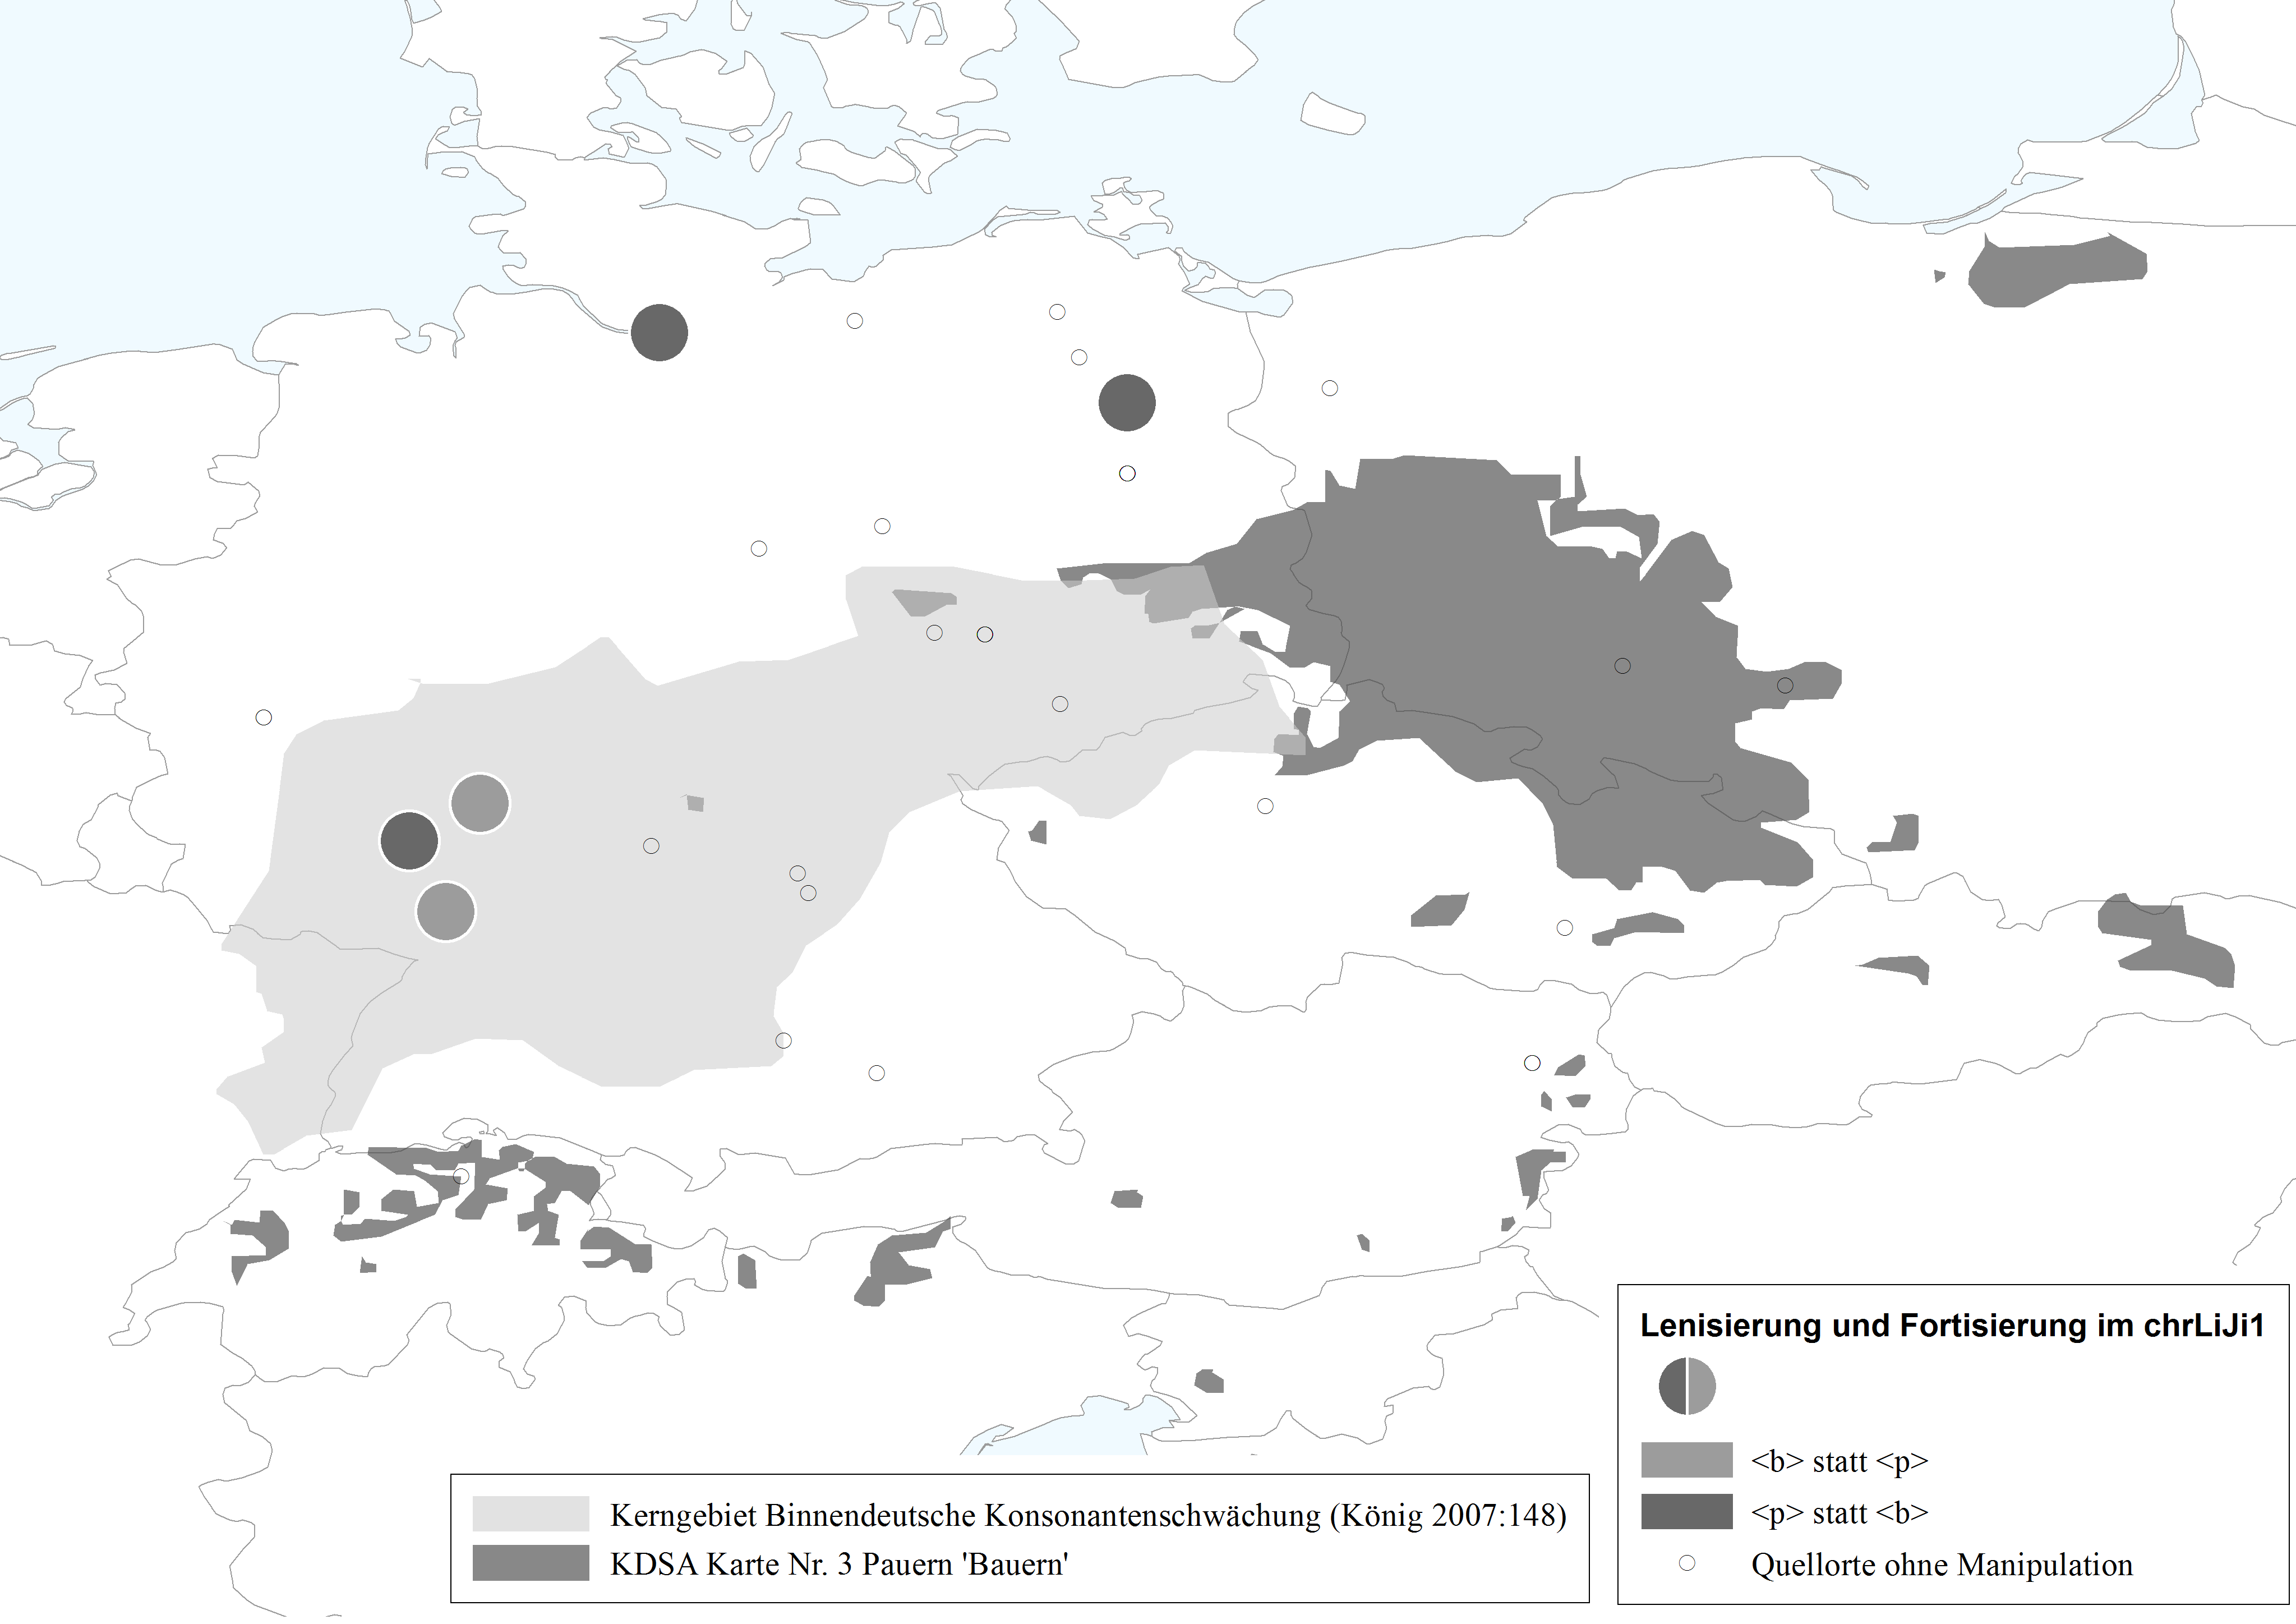
\includegraphics[width=\textwidth]{figures/pb_kdsa.png}
		\caption{\label{kartebpkdsa} Graphien für <p> und <b> im \hai{chrLiJi1} mit \hai{KDSA} Karte Nr. 3 u. \cite[148]{Koenig1978}}
		\end{figure}

  Im Rahmen der sog. binnendeutschen Konsonantenschwächung ist die \isi{Lenisierung} von /p/ > /b/  in einem Großteil der hochdeutschen Mundarten verbreitet, so auch im Rheinfränkischen, wo unsere relevanten Quellen liegen (vgl.\, \citealt[330–346]{Schirmunski1962};\citealt[148f]{Koenig1978}). Nach \cite[221]{Klepsch2004} haben auch die zu den entsprechenden deutschen Dialekten koterritorialen westjiddischen Dialekte an der Konsonantenschwächung teilgenommen. \cite[298–303]{Timm1987} bestätigt dies für das Mitteljiddische insofern, als dass die weit verbreitete fehlende graphematische Homogenität zumindest für die Aufgabe des Fortis-Lenis-Kontrasts spreche.
   


 
 %  \clearpage
 
Das \hai{jüdLiJi1} zeigt die Fortisierung in den zwei Berliner Pamphleten, s. (\ref{bsppbliji2a})--(\ref{bsppbliji2b}). Dies spricht dafür, dass die Fortisierungen im \hai{chrLiJi1} u.\,U. doch ein tatsächliches Phänomen des \hai{{\NWJ}} einfangen.

  \eenumsentence{
\item \textit{praven} \sem{braven} (\hai{PBerlin1}:\,6) \label{bsppbliji2a}

\item \textit{Pauer} \sem{Bauer} (\hai{PBerlin2}:\,1.\,Sp.) \label{bsppbliji2b} \,%rs \, fehlt hinter 1.
}

%Im \hai{LiJi2} finden sich weder Fortisierung noch \isi{Lenisierung} von /b/, /p/.


  
  \subsection{Fortisierung <g> als <k>}\label{kg}
%  %\noindent
Eine weitere Manipulation an Plosiven im \hai{chrLiJi1} ist die Fortisierung von /g/ als /k/ (vgl.\, \citealt[330–346]{Schirmunski1962}). Diese findet sich in 13 Quellen des \hai{chrLiJi1} im  \isi{Anlaut} vor Konsonant und Vokal\footnote{Hier besonders im Partizipialpräfix \textit{ge-}.} (\ref{bspkgliji1}–\ref{bspkgliji7}).

  \eenumsentence{
 \item \textit{klaich} \sem{gleich} (\hai{JK} Breslau, 1810: 35, 52, 57), \textit{Kriek} \sem{Krieg} (\hai{JK} Breslau, 1810: 50) \label{bspkgliji1}
 \item  \textit{kewußt} \sem{gewusst} (\hai{DK} Osterwieck, 1872: 47R)\label{bspkgliji2}
 \item \textit{kegen} \sem{gegen} (\hai{DW} Wien, 1773: 66)\label{bspkgliji3}
 \item \textit{krauß} \sem{groß} (\hai{LR}: 5)\label{bspkgliji4}
 \item  \textit{kehandelt} \sem{gehandelt} (\hai{PF} Augsburg, 1816: 11), \textit{kewesen} \sem{gewesen} (\hai{PF} Augsburg, 1816: 11, 12, 18),  \textit{kesogt} \sem{gesagt} (\hai{PF} Augsburg, 1816: 12),  \textit{Keschmack} \sem{Geschmack} (\hai{PF} Augsburg, 1816: 12, 13),  \textit{kefunden} \sem{gefunden} (\hai{PF} Augsburg, 1816: 12),  \textit{kesehn} \sem{gesehen} (\hai{PF} Augsburg, 1816: 12), \textit{keschlichen} \sem{geschlichen} (\hai{PF} Augsburg, 1816: 12),  \textit{keboten} \sem{geboten} (\hai{PF} Augsburg, 1816: 12), \textit{kesagt} \sem{gesagt} (\hai{PF} Augsburg, 1816: 14, 18),  \textit{kedient} \sem{gedient} (\hai{PF} Augsburg, 1816: 14),  \textit{kescheidt} \sem{gescheit}  (\hai{PF} Augsburg, 1816: 18), \textit{kanz} \sem{ganz} (\hai{PF} Augsburg, 1816: 18) \label{bspkgliji5}
 \item \textit{kraußen} \sem{großen} (\hai{TH} Merseburg, 1820: 97) \label{bspkgliji6}
 \item \textit{kewaltik} \sem{gewaltig} (\hai{VD} Frankfurt, 1916: 15),  \textit{keschrien} \sem{geschrien} (\hai{VD} Frankfurt, 1916: 16) \label{bspkgliji7}

}


Daneben findet sich im \hai{chrLiJi1} die \isi{Auslautverhärtung},\,d.\,h. die Fortisierung der Silbenkoda,\,von /g/ in drei Quellen graphematisiert (\ref{bspkgliji8}–\ref{bspkgliji10}). Bemerkenswert daran ist,\,dass dieses Charakteristikum aller gesprochensprachlichen Varietäten des Deutschen wie auch des Jiddischen im Unterschied zu anderen konsonantischen Merkmalen nur in sehr wenigen Quellen auftaucht.\footnote{Zur \isi{Auslautverhärtung} im Jiddischen und Deutschen vgl.\, \cite[373]{Bin-Nun1973}.} Scheinbar ist dem \hai{{\LiJieins}} in erster Linie weniger an der Hervorhebung der gesprochenen Sprache als vielmehr an den Differenzen des Jiddischen zum Deutschen gelegen.

 \eenumsentence{
\item \textit{lebendik} \sem{lebendig} (\hai{JK} Breslau, 1810: 44, 47), \textit{gesakt} \sem{gesagt} (\hai{JK} Breslau, 1810: 6, 23, 30, 35, 37), \textit{schlaickt} \sem{schlägt} (\hai{JK} Breslau, 1810: 26) \label{bspkgliji8}
\item \textit{gewaltik} \sem{gewaltig} (\hai{PA} Frankfurt, 1834: Titel, 11), \textit{Ufzück} \sem{Aufzüge} (\hai{PA} Frankfurt, 1834: Titel), \textit{zwanzik} \sem{zwanzig} (\hai{PA} Frankfurt, 1834: 10), \textit{geduldik} \sem{geduldig} (\hai{PA} Frankfurt, 1834: 10), \textit{sakt} \sem{sagt} (\hai{PA} Frankfurt, 1834: 87W), \sem{gesagt} (\hai{PA} Frankfurt, 1834: 16, 36, 114) \label{bspkgliji9}
\item  \textit{Keinik} \sem{König} (\hai{VD} Frankfurt, 1916: 15, 18), \textit{wek} \sem{weg} (\hai{VD} Frankfurt, 1916: 18R), \textit{fertik} \sem{fertig} (\hai{VD} Frankfurt, 1916: 20), \textit{gewaltike} \sem{gewaltige} (\hai{VD} Frankfurt, 1916: 14) \label{bspkgliji10}

}


Im \hai{KDSA} finden sich nur im Obersächsischen, wo die generelle Neutralisierung der Fortis und Lenis bei den Plosiven erfolgte \parencite[332]{Schirmunski1962},Streubelege für die Fortisierung im \isi{Anlaut} in den deutschen Varietäten (vgl.  Abbildung \ref{kartekgkdsa}). Es muss jedoch berücksichtigt werden, dass die dem \hai{WA} wie dem \hai{KDSA} zugrundeliegenden Wenkermaterialien bei der Erhebung konsonantischer Daten nicht sehr ergiebig waren (vgl.  \citealt{Bremer1895}). Man kann daher davon ausgehen, dass die karierten Areale de facto weitaus größer sind, als die Daten vermuten lassen. Dennoch kann man in Abbildung \ref{kartekgkdsa} sehen, dass immerhin zwei Quellen im näheren Umfeld zur Fortisierung in den deutschen Mundarten liegen und dadurch beeinflusst sein können. Die übrigen Belege im westmitteldeutschen, bairischen und schlesischen Raum zu beurteilen,  %rs Komma
fällt deutlich schwerer. Es ist möglich, dass dort in den deutschen Dialekten ebenfalls eine Fortisierung vorliegt, deren Interferenzen sich im \hai{{\LiJieins}} niederschlagen oder aber, dass die Autoren durch diese Graphie eine \quein{Andersartigkeit} der jiddischen Dialekte darstellen wollen, die uns entweder nicht aus authentischen Quellen des Westjiddischen bekannt ist oder hier lediglich als literarisches Mittel fungiert, um \quein{Fremdheit} zu erzeugen.

  \begin{figure}
		\centering
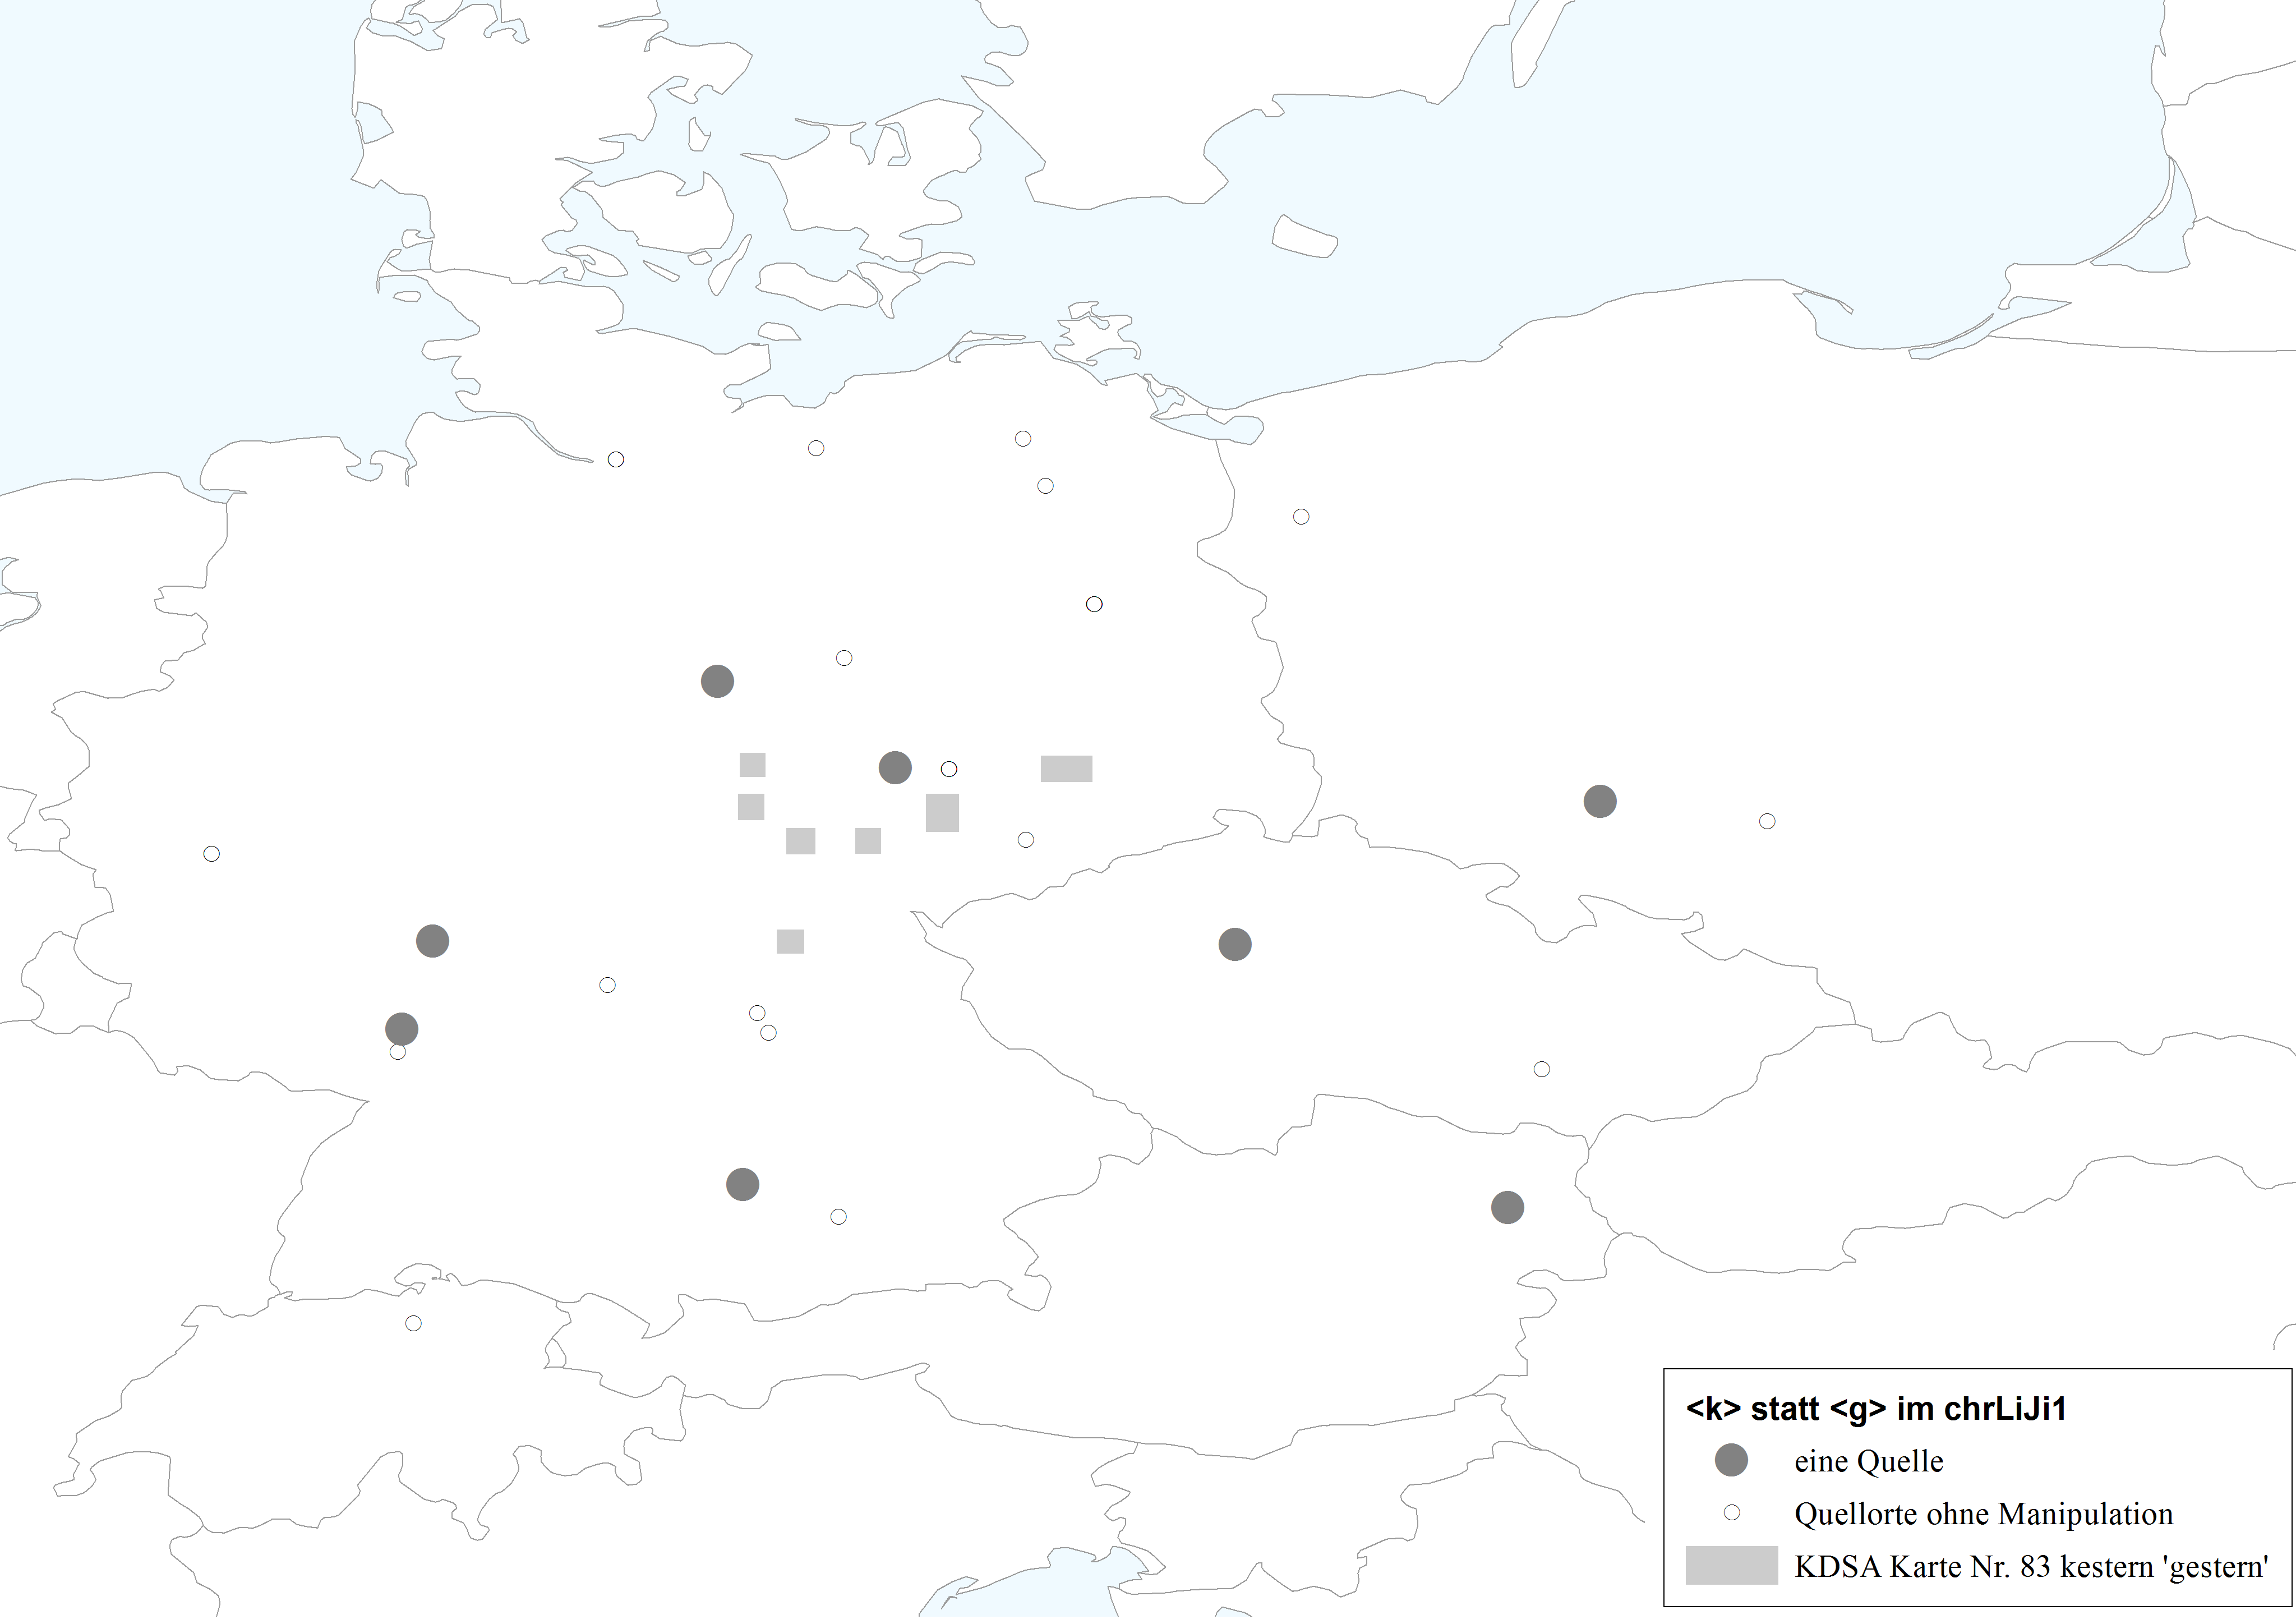
\includegraphics[width=\textwidth]{figures/karte_kg_KDSA.png}
		\caption{\label{kartekgkdsa} <k> für <g> in \isi{Anlaut} im \hai{chrLiJi1} mit \hai{KDSA} Karte Nr. 83}
		\end{figure}

		
		
Die tatsächliche Sprachsituation in den jiddischen Dialekten gestaltet sich wie folgt: Zwar zeigen einige wenige Wörter im modernen \hai{{\OJ}} sogar eine solche Fortisierung,\,z.\,B.\, \RL{קעגן} \textit{kegn} \sem{gegen} (für weitere Bsp. s. \citealt[373]{Bin-Nun1973}). Der einzige Beleg für eine Fortisierung von /g/ im \hai{jüdLiJi1} betrifft genau dieses Lexem: \textit{kegen} \sem{gegen} (\hai{PDebrecen}:\,4, 7), was damit eine ostjiddische Form korrekt wiedergibt. Die Regel ist jedoch im \hai{{\OJ}} der Erhalt des Fortis-Lenis-Kontrastes.  So wird etwa das im \hai{{\LiJi}} oftmals betroffene \textit{ge-}Präfix im Jiddischen immer als stimmhafter velarer Plosiv realisiert.  

Den Daten des \hai{LCAAJ} (Karte Nr. 83) zu Folge, liegt im \hai{ZWJ}, \hai{{\SWJ}} und {\ndl} \hai{{\NWJ}} mit der \isi{Lenisierung} von anlautendem /k/ > /g/ eine gegensätzliche Entwicklung vor (s. Karte in Abbildung \ref{kartekgkdsalcaaj}). Dies ist ein Reflex der sog. \quein{Binnendeutschen Konsonantenschwächung} und in nahezu allen hochdeutschen Dialekten anzutreffen (vgl.\, \citealt[332]{Schirmunski1962}). Die \hai{{\LiJi}}-Quellen bestätigen die westjiddische Situation des \hai{LCAAJ} jedoch nicht: eine \isi{Lenisierung} wird im \hai{{\LiJi}} nirgends verschriftlicht.
		
		
		  \begin{figure}
		\centering
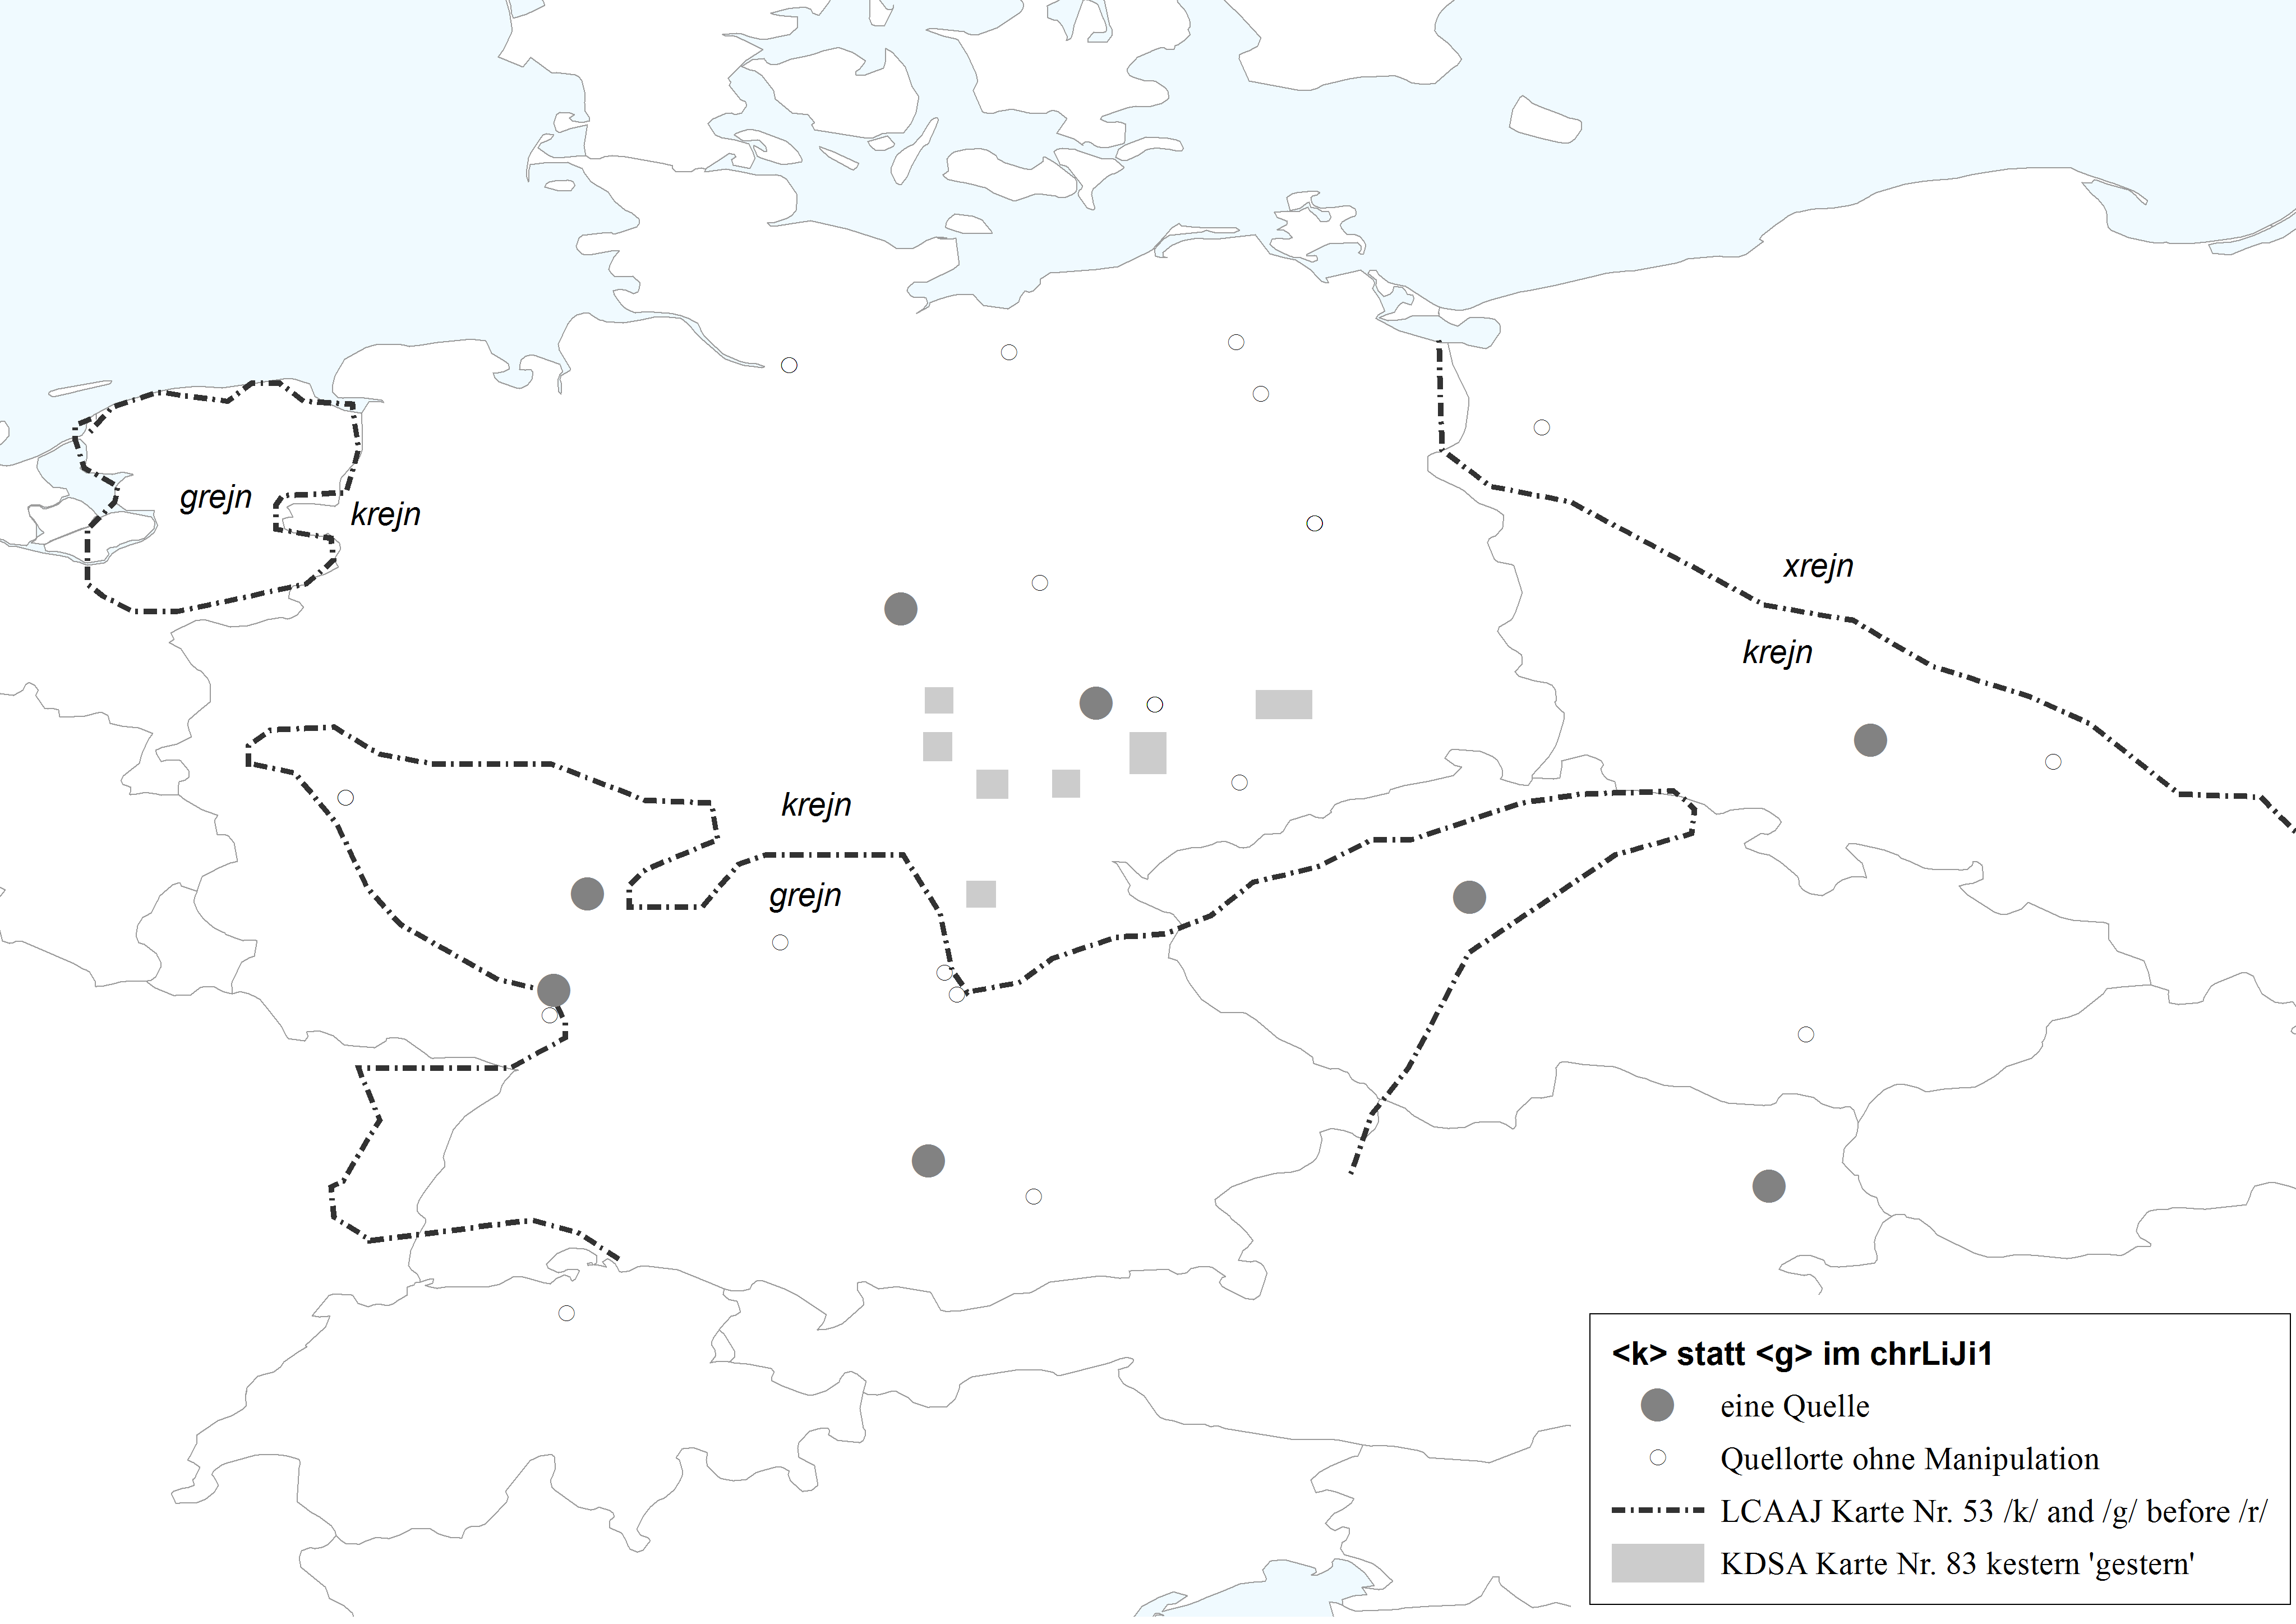
\includegraphics[width=\textwidth]{figures/karte_kg_KDSA_lcaaj.png}
		\caption{\label{kartekgkdsalcaaj} <k> für <g> im \isi{Anlaut}  im \hai{chrLiJi1} mit \hai{KDSA} Karte Nr. 83 und \hai{LCAAJ} Karte Nr. 53}
		\end{figure}



Eine sinnvolle Beurteilung der literaturjiddischen Belege einer Fortisierung von /g/ im \isi{Anlaut} ist letzten Endes nicht möglich, da übersichtliche Daten zur Situation des \isi{Konsonantismus} der deutschen und insbesondere der jiddischen Dialekte fehlen, die Rückschlüsse auf die Authentizität der literaturjiddischen Formen zulassen.
 
   \subsection{Lenisierungen und Fortisierungen als Reflex der oberdeutschen Medienverschiebung}
   %  %\noindent
  Eine mit der 2. \hai{LV} in Verbindung stehende Entwicklung der oberdeutschen Dialekte ist die sogenannte Medienverschiebung von {\ahd} /b/, /d/, /g/ zu /p/, /t/, /k/, die in althochdeutscher Zeit im vorwiegend alemannischen, bairischen und ostfränkischen Raum gewirkt hat (\citealt[131–133]{Szczepaniak2007}). Allerdings ist die Medienverschiebung kein leicht zu fassendes Ereignis und vielfach unsystematisch durchgeführt worden bzw. rückgängig gemacht worden (vgl.\, \citealt[131–133]{Szczepaniak2007}) und die Situation in den oberdeutschen Varietäten ist besonders mit Blick auf deren Diachronie weitestgehend ungeklärt.
 
 Die zuvor aufgezeigten Lenisierungen und Fortisierungen des \hai{chrLiJi1} zeigen dennoch deutliche Ähnlichkeit zu dieser oberdeutschen Entwicklung. Die areale Verteilung der potenziellen Belege der Medienverschiebungen zeigt kein klares Bild: zwar treten Medienverschiebungen gehäuft in Quellen aus dem oberdeutschen Raum auf, darüber hinaus aber auch recht häufig im Norden und Osten (z.\,T. auch Westen) des Untersuchungsgebiets (vgl.\, die Karten in Abbildung \ref{kartedtkdsa}, S.\, \pageref{kartedtkdsa};\ref{kartebpkdsa}, S.\, \pageref{kartebpkdsa} u. \ref{kartekgkdsa}, S.\, \pageref{kartekgkdsa}). Demnach ist nicht auszuschließen, dass die eigene Dialektalität der Autoren in diese Formen einfloss bzw. deren Konzept von oberdeutschen Dialekten, zu denen sie möglicherweise auch das Jiddische zählten.
 
 Doch die Formen des \hai{{\LiJieins}} könnten auch auf einen tatsächlichen westjiddischen Sprachstand referieren. Vieles spricht dafür, dass die Medienverschiebung auch in den zum Oberdeutschen koterritorialen Dialekten des Westjiddischen stattgefunden hat (\hai{LCAAJ} Karte Nr. 53 vgl.\, Abbildung \ref{kartekgkdsalcaaj} S.\, \pageref{kartekgkdsalcaaj}). Hierzu fehlt es jedoch noch an ausführlicheren Untersuchungen.
 
  \subsection{Erhalt von westgermanisch *-\textit{pp}-}

Die in- und auslautende Geminate {\westgerm} *-\textit{pp}- blieb in Ost- und \ili{Westjiddisch} unverändert (\citealt[189]{Kleine2008};\citealt[323–327]{Bin-Nun1973}). Im \hai{chrLiJi1} ist dies in drei Quellen korrekt umgesetzt (\ref{bsp2lv1}–\ref{bsp2lv3}). Dabei liegen die Quellen \hai{FL} (Mannheim, 1778) und \hai{MV} (Berlin, 1862) im Gebiet, das die Entwicklung zu -\textit{pf}- nicht mitgemacht hat (vgl.\, \citealt[64f]{Koenig1978}).\footnote{In einer dieser Quellen, die in den rheinfränkischen Raum verortet wurde, findet sich ein Beleg für unverschobenes {\germ} \textit{-k-} \textit{ick} \sem{ich} (\hai{FL} Mannheim, 1778:\,36), was keinem jiddischen (und auch keinem hochdeutschen) Dialekt entspricht und als einmaliger \quein{Fehler} zu bewerten ist.} Die Belege aus diesen Quellen könnten also auch auf Interferenzen mit den örtlichen deutschen Dialekten zurückgeführt werden. Es findet sich also nur eine Quelle (\hai{SV} München, 1890), bei der mit relativer Sicherheit eine authentische jiddische Form vorliegt.
  
   \eenumsentence{
 \item \textit{Kop} \sem{Kopf} (\hai{FL} Mannheim, 1778: 38) \label{bsp2lv1}
 \item \textit{Köppe} \sem{Köpfe} (\hai{MV} Berlin, 1862: 62,  153) \label{bsp2lv2}
 \item \textit{Knepp} \sem{Knöpfe} (\hai{SV} München, 1890: 2),  \textit{Koppe} \sem{Kopf} (\hai{SV} München,  1890: 3,  5) \label{bsp2lv3}
  
} 

Im  \hai{jüdLiJi1} sind Belege für das Ausbleiben der 2. \hai{LV} bei {\westgerm} -\textit{pp}- deutlich häufiger. Sieben der zehn Quellen zeigen keine Affrikate (Bsp. \,%rs Spatium
\ref{bsp2lv4}–\ref{bsp2lv10}). Diese Quellen sind allesamt im Berliner Raum entstanden, womit Interferenzen mit den deutschen Dialekten nicht auszuschließen sind (vgl.\, \citealt[64f]{Koenig1978}). 
 
  \eenumsentence{
\item \textit{Strümp} \sem{Strümpfe} (\hai{GuS1}: 3), \textit{ausgestoppt} \sem{ausgestopft} (\hai{GuS1}: 4), \textit{Kopp} \sem{Kopf} (\hai{GuS1}: 4) \label{bsp2lv4}

\item  \textit{Köppe} \sem{Köpfe} (\hai{GuS5}: 4), \textit{gehuppt} \sem{gehüpft} (\hai{GuS5}: 4), \textit{kuppernen} \sem{kupfernen} (\hai{GuS5}: 5) \label{bsp2lv5}

\item \textit{Kopp} \sem{Kopf} (\hai{GuS10}: 6, 9, 10, 11), \textit{Schulklopper} \sem{Schulklopfer} (\hai{GuS10}: 9, 11), \textit{Kupperhütchens} \sem{Kupferhüten} (\hai{GuS10}: 10, 11) \label{bsp2lv6}

\item   \textit{zerkloppt} \sem{zerklopft} (\hai{GuS15}: 3R), \textit{vollgestoppt} \sem{vollgestopft} (\hai{GuS15}: 3R)\label{bsp2lv7}

\item \textit{Kopp} \sem{Kopf} (\hai{GuS23}: 9) \label{bsp2lv8}

\item \textit{Tröppcher} \sem{Tropfen} (\hai{PBerlin1}: 2), \textit{Kopp} \sem{Kopf} (\hai{PBerlin1}: 4, 6, 7) \label{bsp2lv9}

\item \textit{Kopp} \sem{Kopf} (\hai{PBerlin2}: 1.Sp.), \textit{Schtrümps/Schtrümpe} \sem{Strümpfe}\\ (\hai{PBerlin2}:\\ 1. Sp., 2. Sp.) \label{bsp2lv10}  %rs   fehlt
}


Wie auch die \isi{Auslautverhärtung} ist dieses,\,orthographisch relativ leicht umsetzbare Phänomen erstaunlich selten im \hai{chrLiJi1} zu finden. Auffallend häufiger sind hingegen Belege im \hai{jüdLiJi1}. In den meisten Fällen stammen die Quellen aus dem sich zwischen Benrather- und Speyrer-Linie befindenden Areal,\,in dem die 2. \hai{LV} an dieser Position wie im Jiddischen unterlassen wurde.



\subsection{Spirantisierung <b> als <w>}\label{bw}
%  %\noindent  
Die Spirantisierung von (insbes. intervokalisch) 
/b/ > /v/ hat große Teile des deutschen Sprachgebiets erfasst (\hai{KDSA} Karten Nr. 23–33,\,bes. 30). Neben dem Niederdeutschen,\,wo {\westgerm} \textit{ƀ} *[v] unverschoben blieb,\,findet  sich die Spirantisierung im gesamten Westmitteldeutschen,\,Niederalemannischen,\,im Nordbairischen Böhmens und vereinzelt im Mittel- und Südbairischen. Im bairischen Raum ist sie seit dem Mittelhochdeutschen schriftlich belegt (\hai{DWB}: \citeyear[Bd. 27,\,Sp. 4]{DeutschesWB}).  \cite[328,\,357]{Bin-Nun1973} stellt fest,\,dass diese Spirantisierung im Jiddischen nur in einzelnen Lexemen und regional gebunden auftritt (\ref{bspOJbw1}–\ref{bspOJbw3}). \cite[357]{Bin-Nun1973} geht bei diesem Phänomen von Einflüssen aus den koterritorialen deutschen Dialekten aus.

 \eenumsentence{
\item Standard {\oj} \RL{{א\makebox(-1.25,-1.25)[r]{\libertineGlyph{uni05B8}}}וונט} \textit{ovnt} \sem{Abend} \label{bspOJbw1} %format!  Diakritikum
\item {\oj} Dialekte \textit{oiwm} \sem{oben}  \parencite[356]{Bin-Nun1973};Standard {\oj} \RL{איבער} \textit{iber} \label{bspOJbw2}
\item Elsässer {\wj} \textit{lîwi} \sem{liebe} \parencite[356]{Bin-Nun1973};Standard {\oj} \RL{ליבער} \textit{liber}\label{bspOJbw3}
}

Die Verbreitung der Spirantisierung im \hai{Westjiddischen} erfasst nach Beranek (\hai{WjSA}: Karte Nr. 33) nur ein kleines Gebiet im äußersten Westen des \hai{ZWJ} und \hai{{\SWJ}}. Spätere Ausbreitungen dieser Form auf östliche Varietäten des \hai{{\WJ}} werden hier jedoch auch (durch diffuse Pfeile angedeutet) angenommen. Der \hai{LCAAJ} (Karte Nr. 51) setzt ein deutlich größeres Areal im westlichen \hai{{\WJ}} an (vgl.\,Abbildung \ref{kartebwlcaaj}). Dieses Areal entspricht weitestgehend der Verbreitung dieses Phänomens in den deutschen Mundarten (\hai{KDSA} Karten Nr. 23–33, bes. 30). \citeauthor{Bin-Nun1973}s (\citeyear[357]{Bin-Nun1973}) Hypothese eines deutschen Einflusses auf das Jiddische ist zumindest im \hai{{\WJ}} nicht auszuschließen.
  
Im \hai{chrLiJi1} finden sich lediglich zwei Quellen, die sich der Spirantisierung als Markierungsmittel bedienen (\ref{bspLiJibw1}–\ref{bspLiJibw3}). Diese liegen im bzw. nahe dem Gebiet, für das der \hai{LCAAJ} die Spirantisierung verzeichnet (vgl.\, Abbildung \ref{kartebwlcaaj}). Für das \hai{jüdLiJi1}, dessen Quellen im östlichen \hai{{\WJ}} liegen, ist nur ein singulärer Beleg in der westlichsten aller Quellen zu finden (\ref{bspLiJibw3}).

 \eenumsentence{
\item \textit{nowel} \sem{nobel} (\hai{SV} München,\,1890:\,3) \label{bspLiJibw1}
\item \textit{hewe} \sem{haben} (\hai{VD} Frankfurt,\,1916:\,14,\,15,\,17,\,18,\,20),\,\textit{iweraal} \sem{überall} (\hai{VD} Frankfurt,\,1916:\,15,\,18),\,\textit{begewe} \sem{begeben} (\hai{VD} Frankfurt,\,1916:\,15R,\,20R),\, \textit{derneewe} \sem{daneben} (\hai{VD} Frankfurt,\,1916:\,15R),\, \textit{iwle} \sem{übler} (\hai{VD} Frankfurt,\,1916:\,21),\, \textit{verreiwe} \sem{verreiben} (\hai{VD} Frankfurt,\,1916:\,22R),\, \textit{schreiwe} \sem{schreiben} (\hai{VD} Frankfurt,\,1916:\,22R),\,\textit{liewender} \sem{liebender} (\hai{VD} Frankfurt,\,1916:\,22) \label{bspLiJibw2}
\item \textit{Struwelpeter} \sem{Strubbelpeter} (\hai{PAlsleben}:\,Titel) \label{bspLiJibw3}
%\item \textit{uwnt} \sem{Abend} %(\hai{WWR}:\,14,\,29,\,66,\,20,\,76,\,112,\,130,\,144,\,146) \label{bspLiJibw4} 
 
 }
 
		  \begin{figure}
		\centering
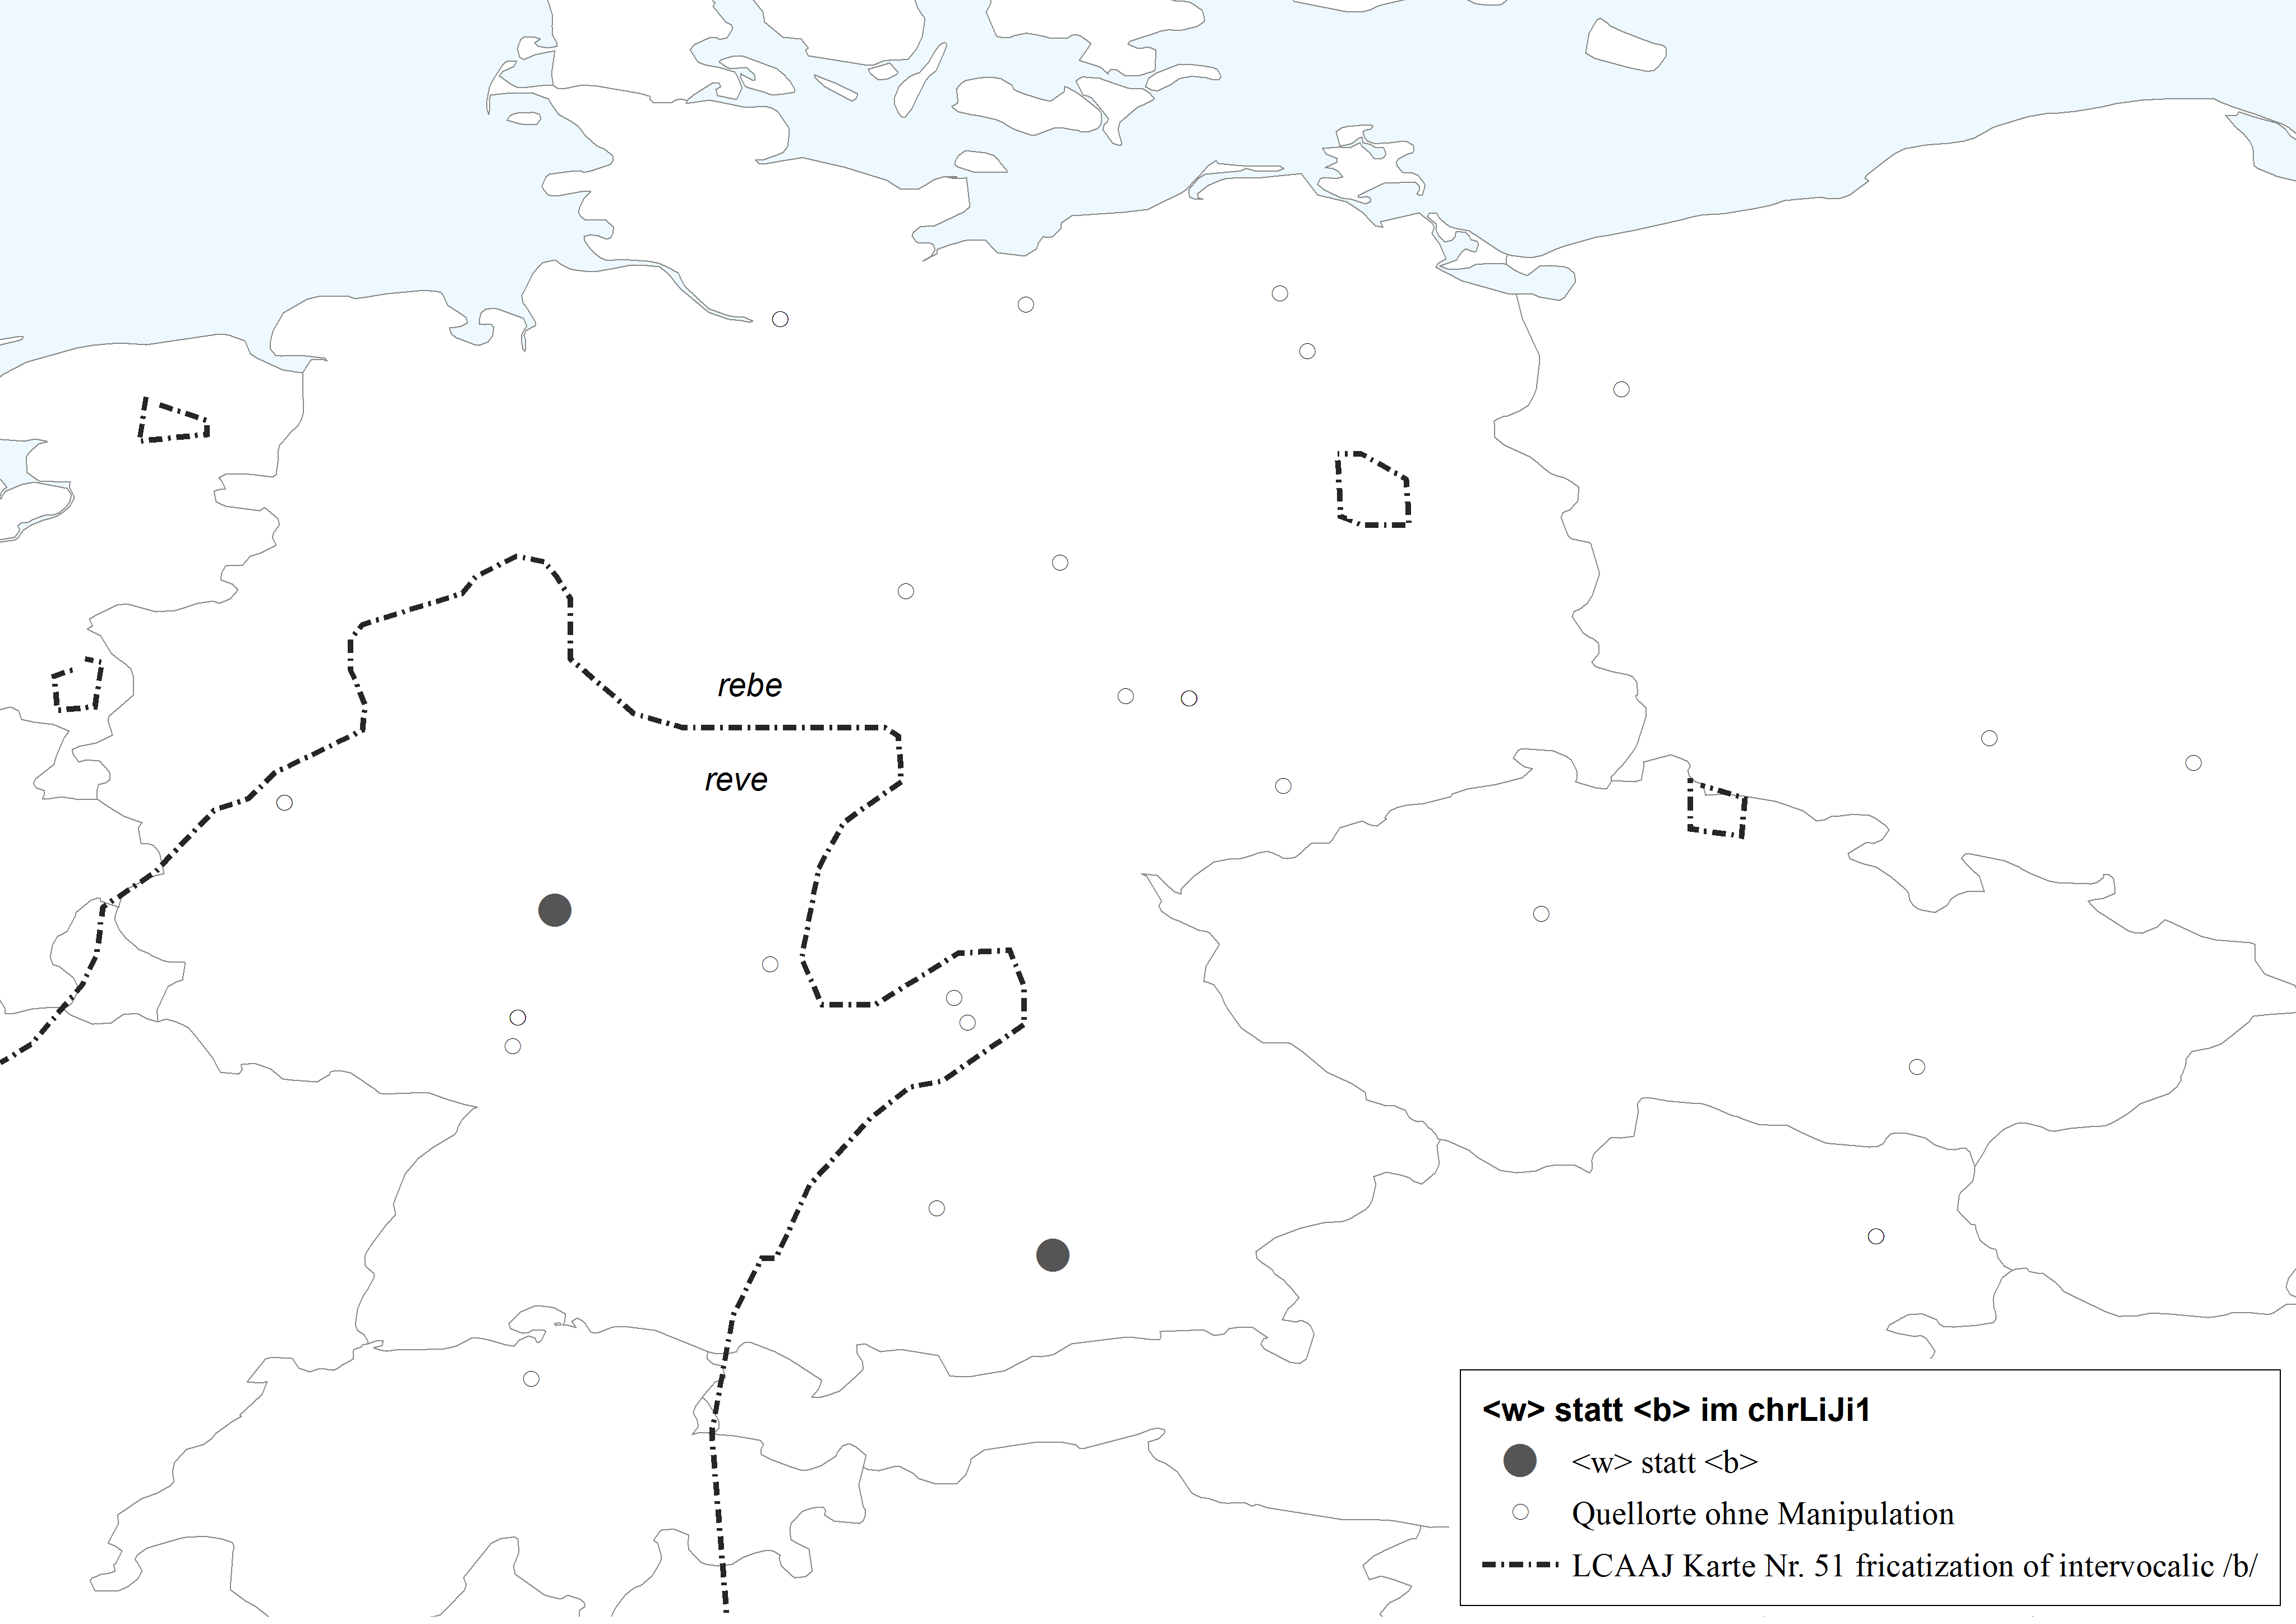
\includegraphics[width=\textwidth]{figures/karte_bw_lcaaj51_vers2_2.png}
		\caption{\label{kartebwlcaaj} <w> für <b> im \hai{chrLiJi1} mit \hai{LCAAJ} Karte Nr. 51}
\end{figure}

		
        \section{Diachrone und diatopische Verteilung phonologischer Manipulationen}\label{fazitphon}
 
%\noindent
 
 Von den insgesamt 26\footnote{Ausgenommen wurde hier die Hyperkorrektur von {\mhd} \textit{î} (\hai{V34}) als <a>,\,<ah>,\,<aa>,\,da es sich hierbei um eine sekundäre Interferenz mit der Monophthongierung von {\mhd} \textit{ei} (V24) handeln kann (oder aber auch eine zentralostjiddische Form darstellen kann). Einzeln Eingang in die Zählung haben hingegen die Zusammenfälle von \hai{V24} und \hai{V44} und von {\mhd} \textit{ê} und \textit{œ} gefunden.} untersuchten phonologischen Strategien des \hai{chrLiJi1} werden in einer Quelle (\hai{VD} Frankfurt,\,1916) maximal 17 eingesetzt (vgl.\,Tabelle \ref{tblphonall}). Der Mittelwert beträgt 6,78  Phänomene  pro Quelle ({$\sigma$}\,4,15). Dies ist ein erstaunlich hoher Durchschnitt.%;\, besonders im Vergleich mit der Lexik, die eine vergleichsweise geringe Rolle im \hai{chrLiJi1} spielt.
  
  \begin{table}[p]
\centering
		\begin{tabular}{lr}
		\lsptoprule
	\textbf{Quellen} & \textbf{phon. Phänomene} \\  \midrule
 \hai{VD} & 17 \\
\hai{SV} & 16\\
\hai{TH}, \hai{MV} & 14\\
\hai{PA} & 13\\
\hai{GW } & 12\\
 \hai{PF}, \hai{AJ} & 11\\
\hai{SS}, \hai{DW},  \hai{AD}, \hai{MS}, \hai{AK} &10\\
\hai{JP},  \hai{PG}, \hai{JK}, \hai{FE} & 9\\
\hai{DG}, \hai{NW}, \hai{AO}  & 8\\
\hai{GP}, \hai{AT}, \hai{BW}, \hai{WA} & 7\\
\hai{UT}, \hai{DK},  \hai{LM}, \hai{FL}, \hai{OF}, \hai{PM}, \hai{IA}, \hai{LS}  & 6\\
\hai{LB}, \hai{EJ}, \hai{DP}  & 5\\
\hai{PL}, \hai{HJ} & 4\\
\hai{LR} & 3\\
\hai{VE}, \hai{AH},  \hai{BS}, \hai{FS}, \hai{EV}, \hai{PP}, \hai{BP} & 2\\
\hai{SB}, \hai{LP}, \hai{FM}, \hai{SH}, \hai{JD} &1\\ \lspbottomrule
  
  
  	
  \end{tabular} 
		 \caption{Anzahl phonologischer Manipulationen im \hai{chrLiJi1}}
		 \label{tblphonall}
		 \end{table}  
  


Das Diagramm in Abbildung \ref{phonall} zeigt, wie viele phonologische Phänomene pro Quelle eingesetzt werden. Quellen mit besonders vielen phonologischen Markierungen finden sich dabei zwischen 1820 und 1830. Aber auch einige der späteren Quellen ab 1890 zeichnen sich durch eine besondere Vielfalt phonologischer Manipulationen aus.
  
\begin{figure}[p]
  \fittable{
	\begin{tikzpicture}
		\begin{axis}[width=1.02\textwidth,height=0.2\textheight,
		legend style={at={(1,1)},xshift=+0.2cm, yshift=-0cm,anchor=north west,nodes=left},
			%title={Funktionstypen des sp\"aten Westjiddisch},
			xtick={1700, 1725, 1750, 1775, 1800, 1825, 1850, 1875, 1900, 1925, 1950, 1975}, ytick=,
			x tick label style={/pgf/number format/1000 sep=}, 
			y tick label style={/pgf/number format/1000 sep=},
			%extra y ticks={456.1, 1022.4},
			%extra y tick labels={{456,1},{1022,4}},
			extra y tick style={grid=major,
				tick label style={, ,}},
				ymin=0.7,
				ymax=19.1,
			ylabel={Phänomene},
			enlarge x limits=0.03]	
	
			
\addplot [thick] table [x=jahr, y=SUMME] {figures/ALLE_summe1_dia.txt};%1


		\end{axis}
	\end{tikzpicture}
}
	\caption{Quantität phonologischer Markierungen im \hai{chrLiJi1}}
	\label{phonall}	
\end{figure}
 
 \largerpage
 Vier\footnote{Dabei handelt es sich um die Monophthongierungen von \hai{V24} und \hai{V44} zu /a\textlengthmark/, sowie deren \isi{Zusammenfall} und die Diphthongierung von \hai{V42} zu /au/, /ou/.} für das Westjiddische charakteristische phonologische Eigenschaften werden von elf Quellen eingesetzt;\, acht Quellen hingegen zeigen keines dieser Phänomene. Der Mittelwert liegt hier bei 2,37  Phänomenen  pro \hai{chrLiJi1}-Quelle ({$\sigma$}\,1,17). Wie die Verteilung in Abbildung \,%rs "Abbildung" ergänzen
 \ref{phonwjall} zeigt, ist weder eine Abnahme westjiddischer Phänomene im Verlauf des 19. Jahrhunderts zu verzeichnen, noch eine Phase erkennbar, \,%rs ,
 in der westjiddische Formen im \hai{chrLiJi1} präsenter sind als sonst. Es ist zwischen 1800 und 1875 eine generell hohe Dichte an authentisch westjiddischen phonologischen Phänomenen festzustellen, deren geringer Schwund nach 1875 vorwiegend der fehlenden Korpusdichte im letzten Drittel des 19. Jahrhunderts geschuldet ist. Ab 1875 finden sich verhältnismäßig weniger Quellen, die diese authentischen Phänomene belegen. Man könnte dies auch generell damit in Verbindung setzen, dass ab dieser Zeit \ili{Westjiddisch} nur mehr marginal in der deutschen Sprachlandschaft präsent war.  
 
 \begin{figure}[p]
	\begin{tikzpicture}
		\begin{axis}[width=1.02\textwidth,height=0.2\textheight,
		legend style={at={(1,1)},xshift=+0.2cm, yshift=-0cm,anchor=north west,nodes=left},
			%title={Funktionstypen des sp\"aten Westjiddisch},
			xtick={1700, 1725, 1750, 1775, 1800, 1825, 1850, 1875, 1900, 1925, 1950, 1975}, ytick=,
			x tick label style={/pgf/number format/1000 sep=}, 
			y tick label style={/pgf/number format/1000 sep=},
			%extra y ticks={456.1, 1022.4},
			%extra y tick labels={{456,1},{1022,4}},
			extra y tick style={grid=major,
				tick label style={, ,}},
				ymin=0.7,
				ymax=4.8,
			ylabel={Phänomene},
			enlarge x limits=0.03]	
	
			
\addplot [thick] table [x=jahr, y=wj_all_phon] {figures/phon_wj_dia.txt};%1


		\end{axis}
	\end{tikzpicture}
	\caption{Quantität \textit{korrekt} imitierter westjiddischer phonologischer Markierungen im \hai{chrLiJi1}}
	\label{phonwjall}	
\end{figure}

 

Insbesondere die vokalischen Manipulationen treten gemeinsam und über den untersuchten Zeitraum hinweg kontinuierlich auf, wie das Streudiagramm in Abbildung \ref{phonwjallstreu} zeigt. Konsonantische Phänomene hingegen kommen besonders im \hai{chrLiJi1} ab der zweiten Hälfte des 19. Jahrhunderts auf. So sind die Quellen zwischen 1840 und 1875 besonders vielfältig bezüglich der phonologischen Markierung. Die kartographische Darstellung in Abbildung \ref{karteplosive} zeigt, dass konsonantische Manipulationen neben dem rheinfränkischen Raum, wo die entsprechenden Phänomene auch in den örtlichen deutschen Dialekten verbreitet sind, besonders häufig im (Nord-)Osten auftauchen. Dies betrifft insbesondere die späteren Quellen.

\begin{figure} 
\farbgrafik

	\begin{tikzpicture}

		\begin{axis}[only marks, width=0.82\textwidth,height=0.68\textheight,
		legend style={at={(1,1)},xshift=+0.2cm, yshift=-0cm,anchor=north west,nodes=left},
			%title={Funktionstypen des sp\"aten Westjiddisch},
			xtick={1700, 1725, 1750, 1775, 1800, 1825, 1850, 1875, 1900, 1925, 1950, 1975}, ytick=\empty,
			x tick label style={/pgf/number format/1000 sep=}, 
			y tick label style={/pgf/number format/1000 sep=},
			%extra y ticks={456.1, 1022.4},
			%extra y tick labels={{456,1},{1022,4}},
			extra y tick style={grid=major,
				tick label style={, ,}},
				ymin=0.51,
				ymax=24.9,
			ylabel={Phänomene},
			enlarge x limits=0.03]	
\addplot [mark=*, Fuchsia] table [x=jahr, y=wb] {figures/all_wb_24.txt};\addlegendentry{<w> statt <b>}
\addplot [mark=*, BrickRed] table [x=jahr, y=LVp] {figures/all_LVp_23.txt};\addlegendentry{{\germ} -\textit{pp}-}
\addplot [mark=*, MidnightBlue] table [x=jahr, y=kg] {figures/all_kg_22.txt};\addlegendentry{<k> statt <g>}
\addplot [mark=*, black] table [x=jahr, y=bp] {figures/all_bp_21.txt};\addlegendentry{<b> statt <p>}
\addplot [mark=*, Thistle] table [x=jahr, y=pb] {figures/all_pb_20.txt};\addlegendentry{<p> statt <b>}
 \addplot [mark=*, LimeGreen] table [x=jahr, y=td] {figures/all_td_19.txt};\addlegendentry{<t> statt <d>}
\addplot [mark=*, ProcessBlue] table [x=jahr, y=dt] {figures/all_dt_18.txt};\addlegendentry{<d> statt <t>}
\addplot [mark=*, Maroon] table [x=jahr, y=s] {figures/all_s_z_17.txt};\addlegendentry{<s> statt <z>}
\addplot [mark=*, Melon] table [x=jahr, y=sz] {figures/all_sz_z_16.txt};\addlegendentry{<ß> statt <z>}
 \addplot [mark=*, RoyalPurple] table [x=jahr, y=scht_anlaut] {figures/all_scht_an_15.txt};\addlegendentry{<scht> (\isi{Anlaut})}
\addplot [mark=*, YellowGreen] table [x=jahr, y=scht_auslaut] {figures/all_scht_aus_14.txt};\addlegendentry{<scht> (\isi{Auslaut})}
\addplot [mark=*, CarnationPink] table [x=jahr, y=oe_i] {figures/all_oe_i_13.txt};\addlegendentry{ö > i}
 \addplot [mark=*, orange] table [x=jahr, y=oe_e] {figures/all_oe_e_12.txt};\addlegendentry{ö > e}
\addplot [mark=*, SkyBlue] table [x=jahr, y=ue_e] {figures/all_ue_e_11.txt};\addlegendentry{ü > e}
\addplot [mark=*, Dandelion] table [x=jahr, y=ue_i] {figures/all_ue_i_10.txt};\addlegendentry{ü > i}
\addplot [mark=*, ForestGreen] table [x=jahr, y=palat] {figures/all_palat_9.txt};\addlegendentry{/u/ > /y/}
 \addplot [mark=*, magenta] table [x=jahr, y=u_o] {figures/all_u_o_8.txt};\addlegendentry{u > o}
\addplot [mark=*, CornflowerBlue] table [x=jahr, y=o_u] {figures/all_o_u_7.txt};\addlegendentry{o > u}
\addplot [mark=*, teal] table [x=jahr, y=V12] {figures/all_v12_6.txt};\addlegendentry{\textit{a}-Verdumpfung}
\addplot [mark=*, purple] table [x=jahr, y=v34] {figures/all_v34_5.txt};\addlegendentry{\hai{V34} ({\mhd} \textit{iu})}
 \addplot [mark=*, YellowOrange] table [x=jahr, y=V22] {figures/all_v22_4.txt};\addlegendentry{\hai{V22} ({\mhd} \textit{ê}/ \textit{œ})}
\addplot [mark=*, green] table [x=jahr, y=V42auou] {figures/all_v42_3.txt};\addlegendentry{\hai{V42} ({\mhd} \textit{ô})}
\addplot [mark=*, cyan] table [x=jahr, y=V44] {figures/all_v44_2.txt};\addlegendentry{\hai{V44} ({\mhd} \textit{ou})}
\addplot [mark=*, red] table [x=jahr, y=V24] {figures/all_v24_1.txt};\addlegendentry{\hai{V24} ({\mhd} \textit{ei})}
		\end{axis}
	\end{tikzpicture}
	\caption{Phonologische Markierungen im \hai{chrLiJi1}}
	\label{phonwjallstreu}	
\end{figure} 
 
 
 
 		
		  \begin{figure}[p]
		 
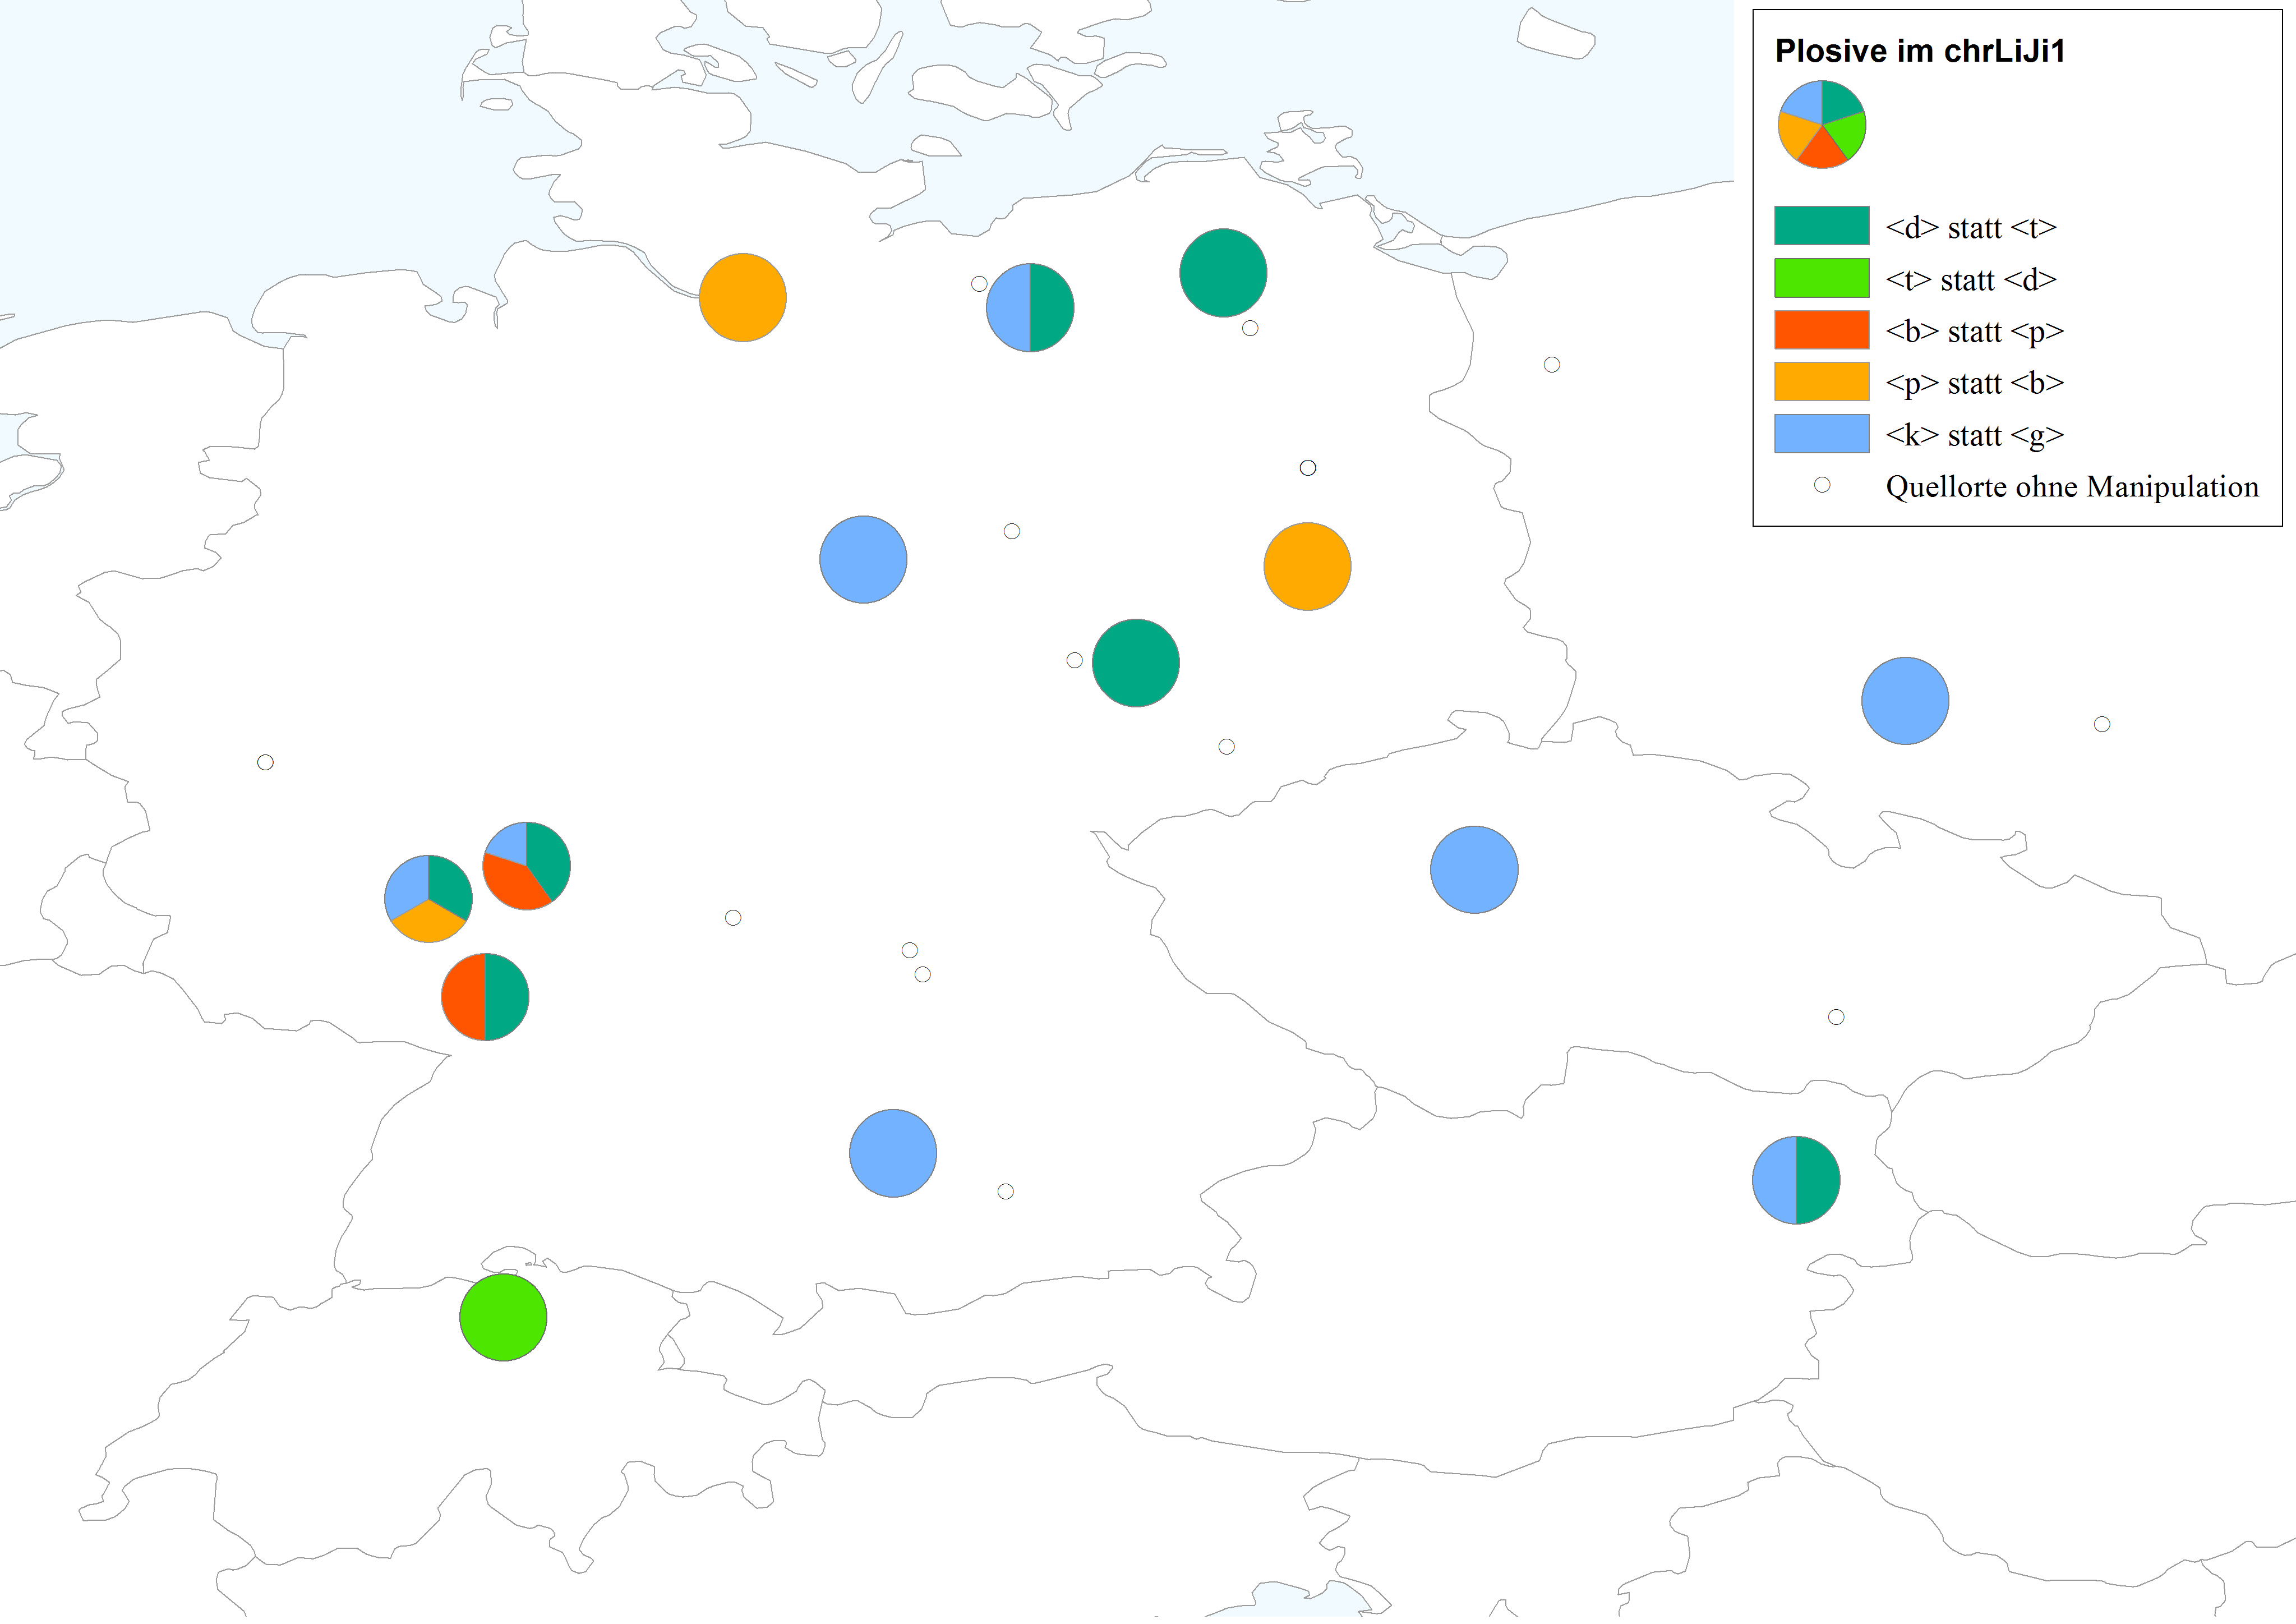
\includegraphics[height=.4\textheight]{figures/karte_plosive.png}
		\caption{\label{karteplosive} Orthographische Auffälligkeiten der \isi{Plosive} im \hai{chrLiJi1}}
		\end{figure}


\begin{figure} 
		 
\fittable{
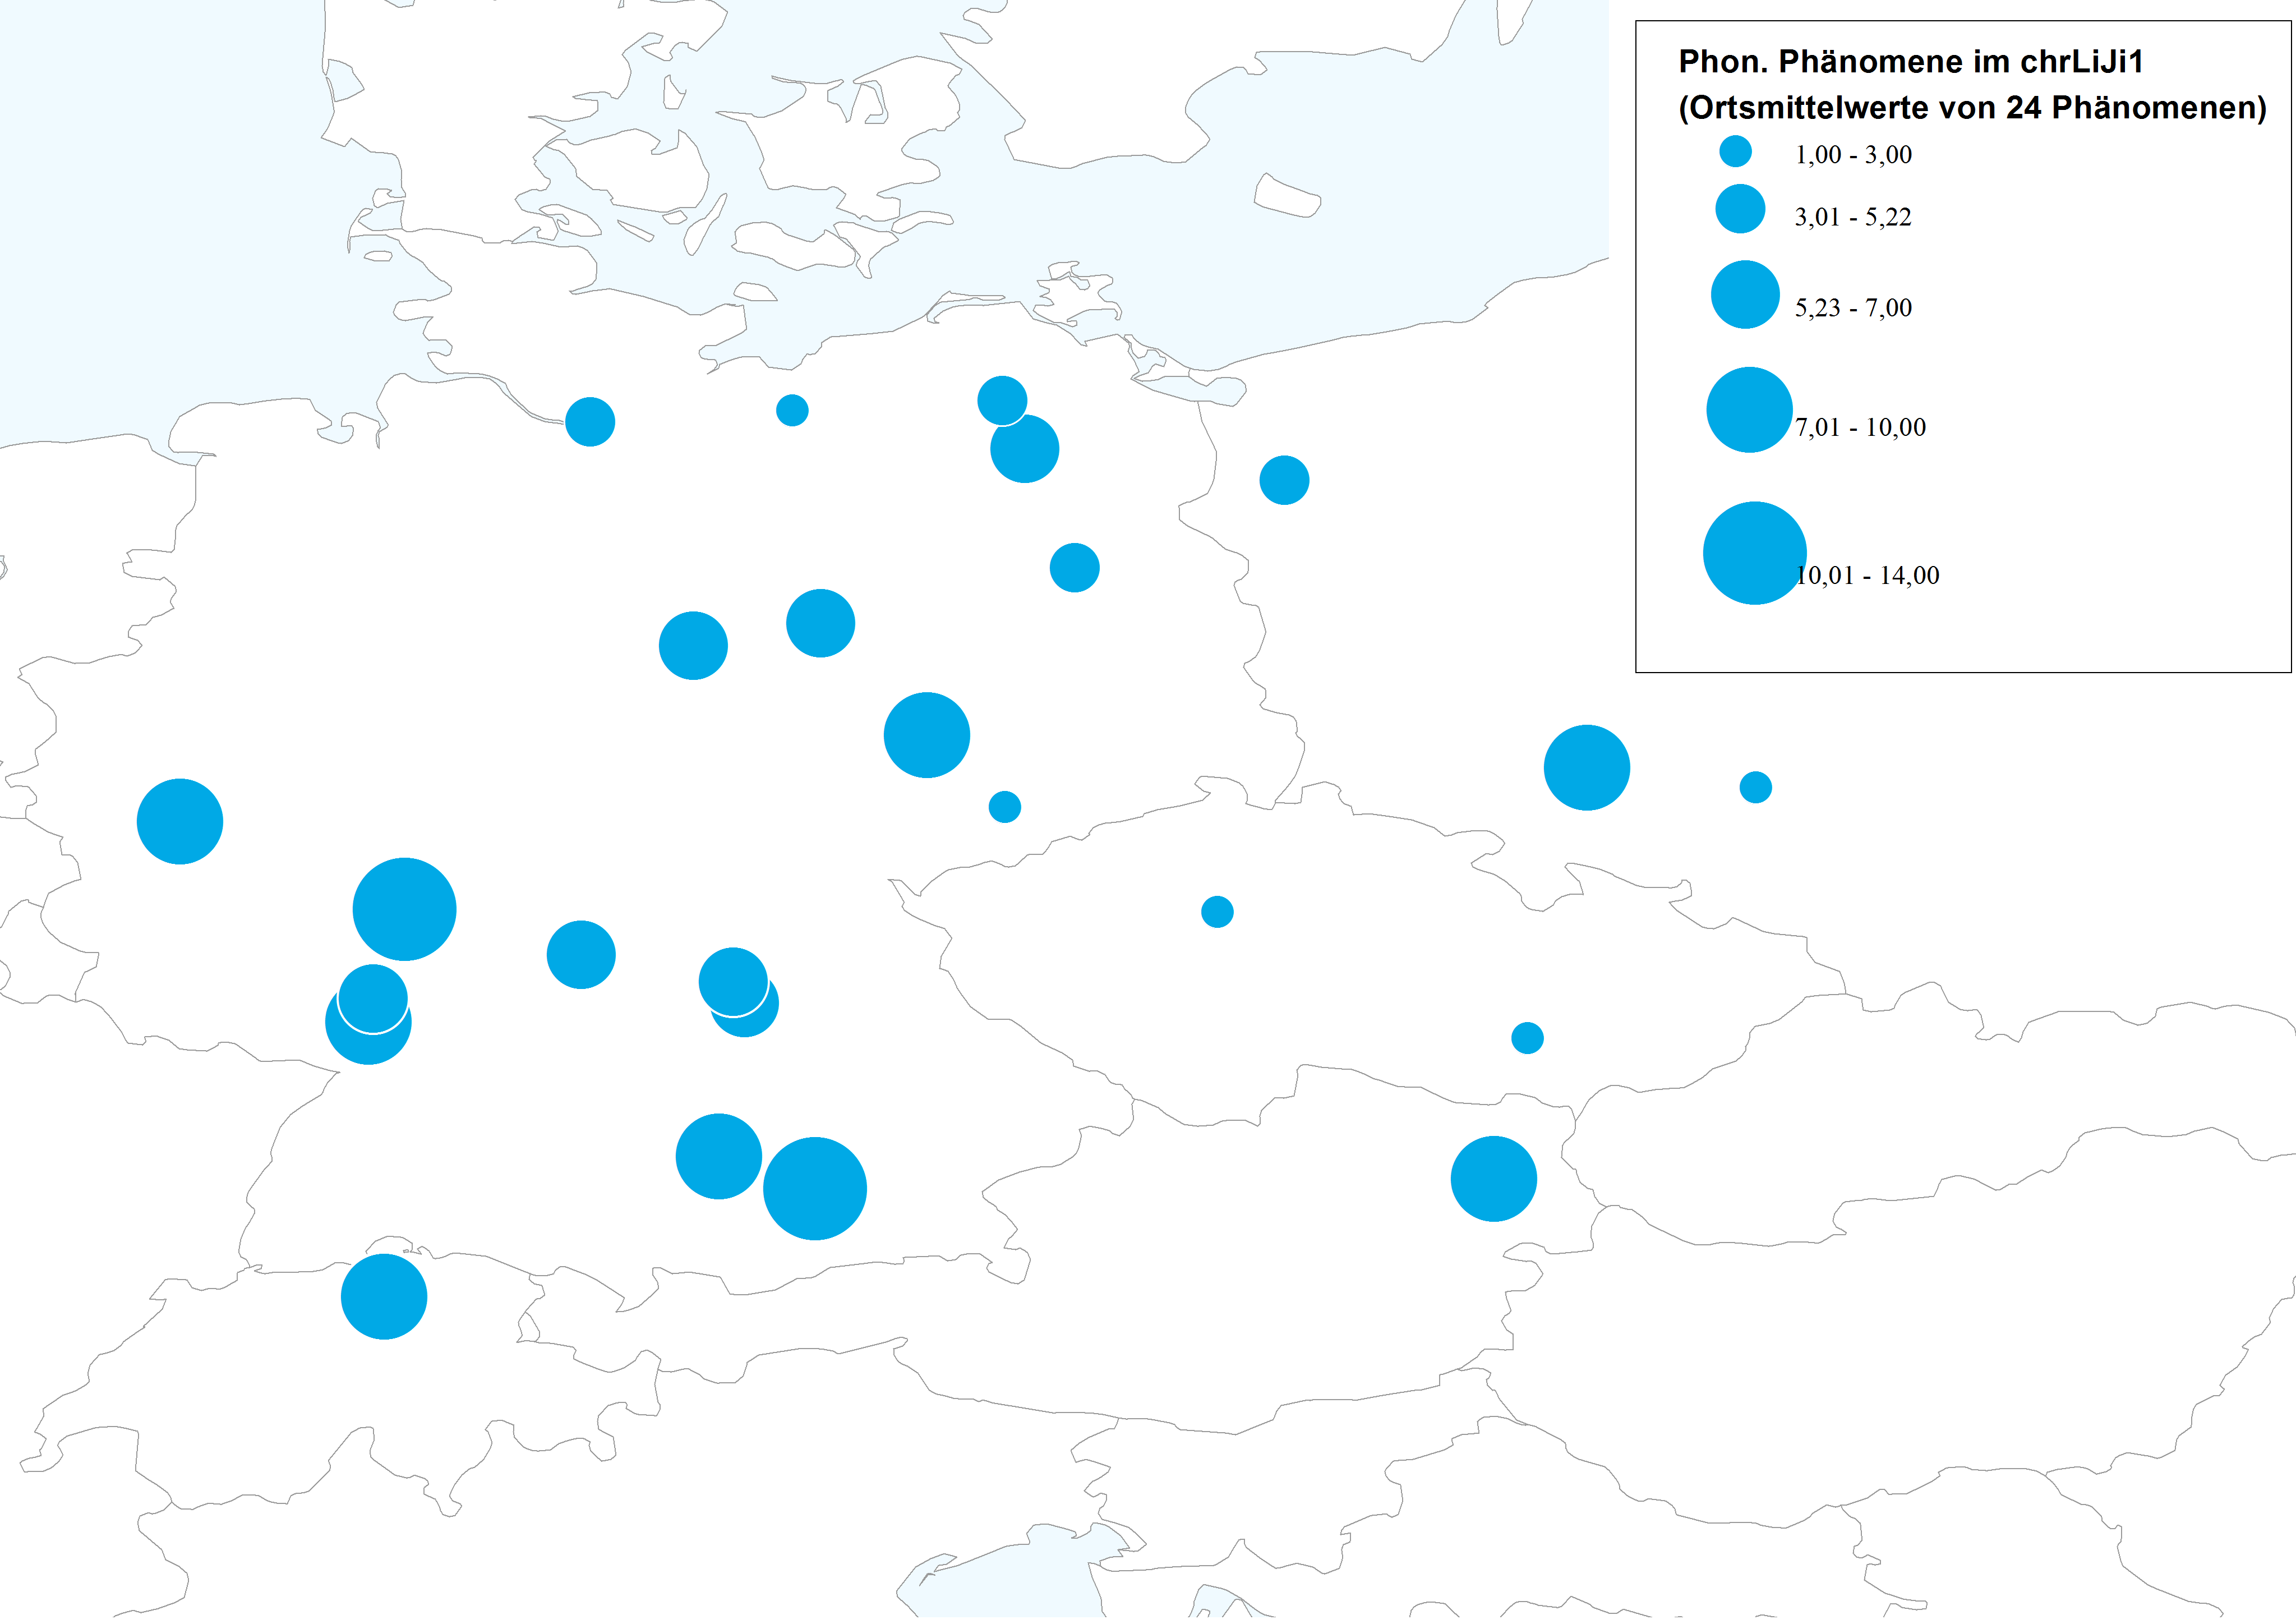
\includegraphics[height=.45\textheight]{figures/phon_chrliji1.png}
}
		\caption{\label{lijiphon} Summe phonologischer Phänomene im \hai{chrLiJi1} (Ortsmittelwerte)}
\end{figure}

  
 
\begin{figure}[p]
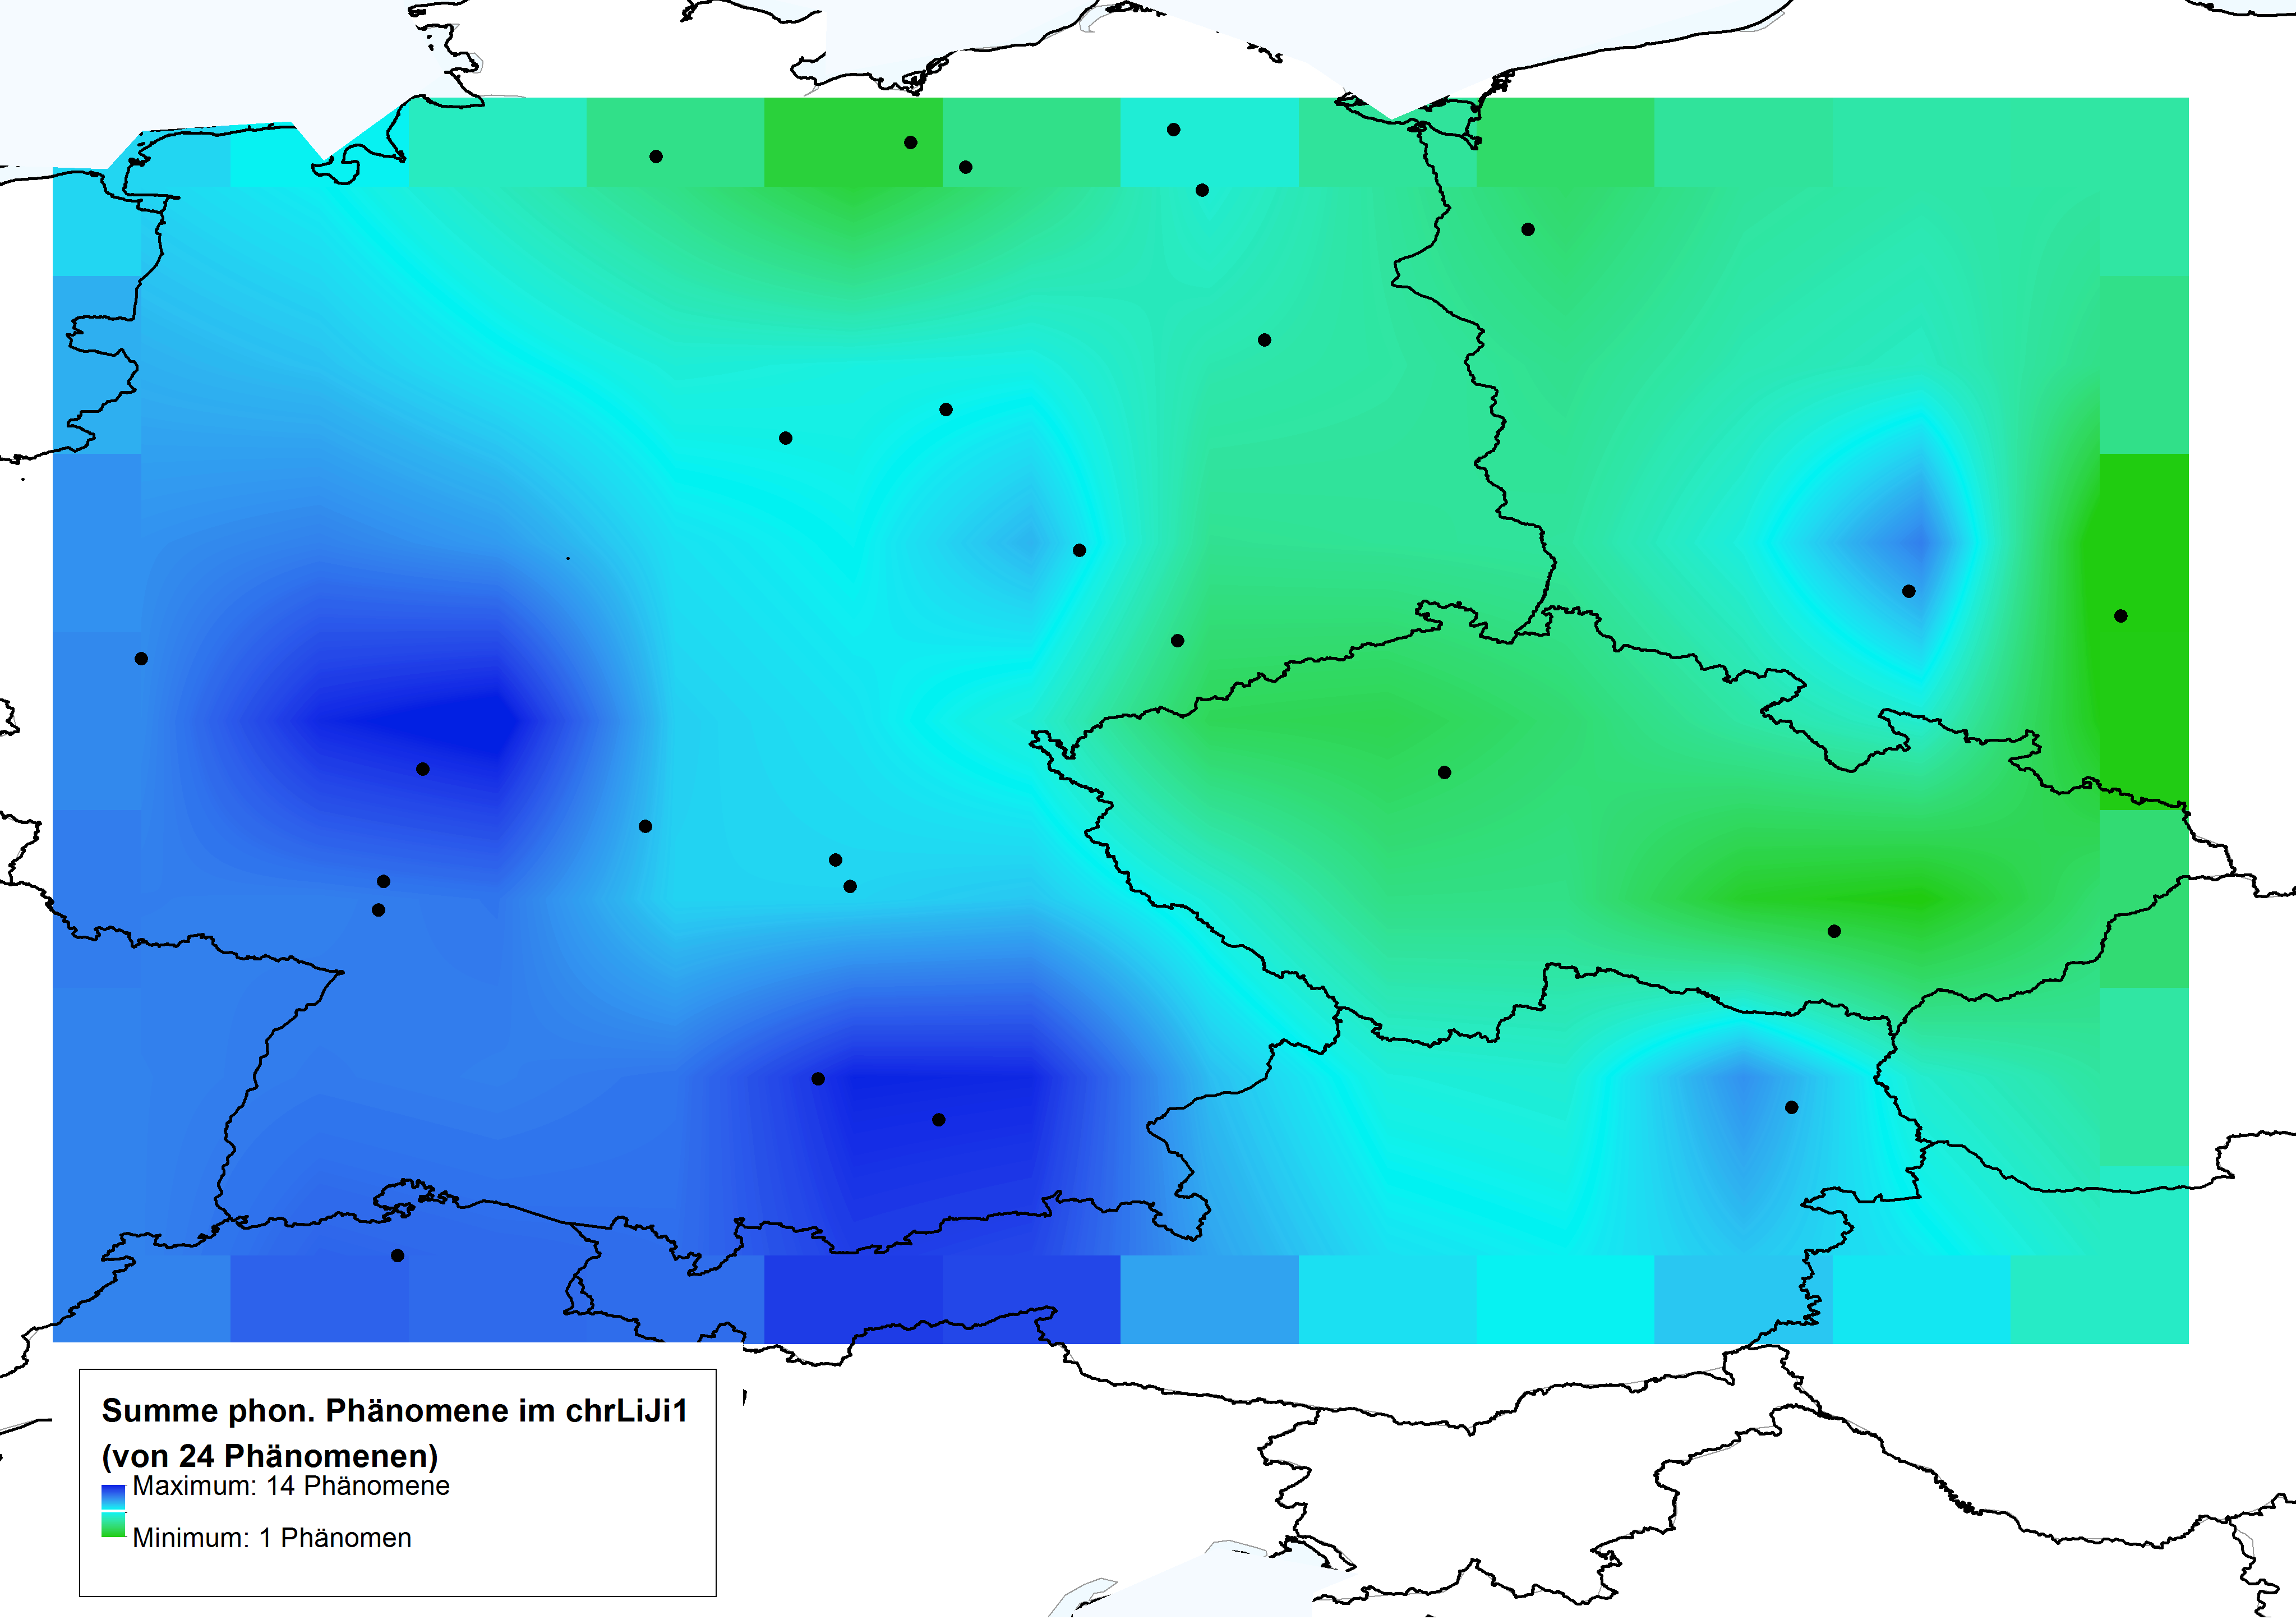
\includegraphics[height=.45\textheight]{figures/phon_liji_nurIDW_PUNKT.png}
		\caption{\label{kartelijiIDW}Darstellung der Abstufungen der Summe phonologischer Phänomene im \hai{chrLiJi1} (\hai{IDW})}
		\end{figure}

 \begin{figure}[p]
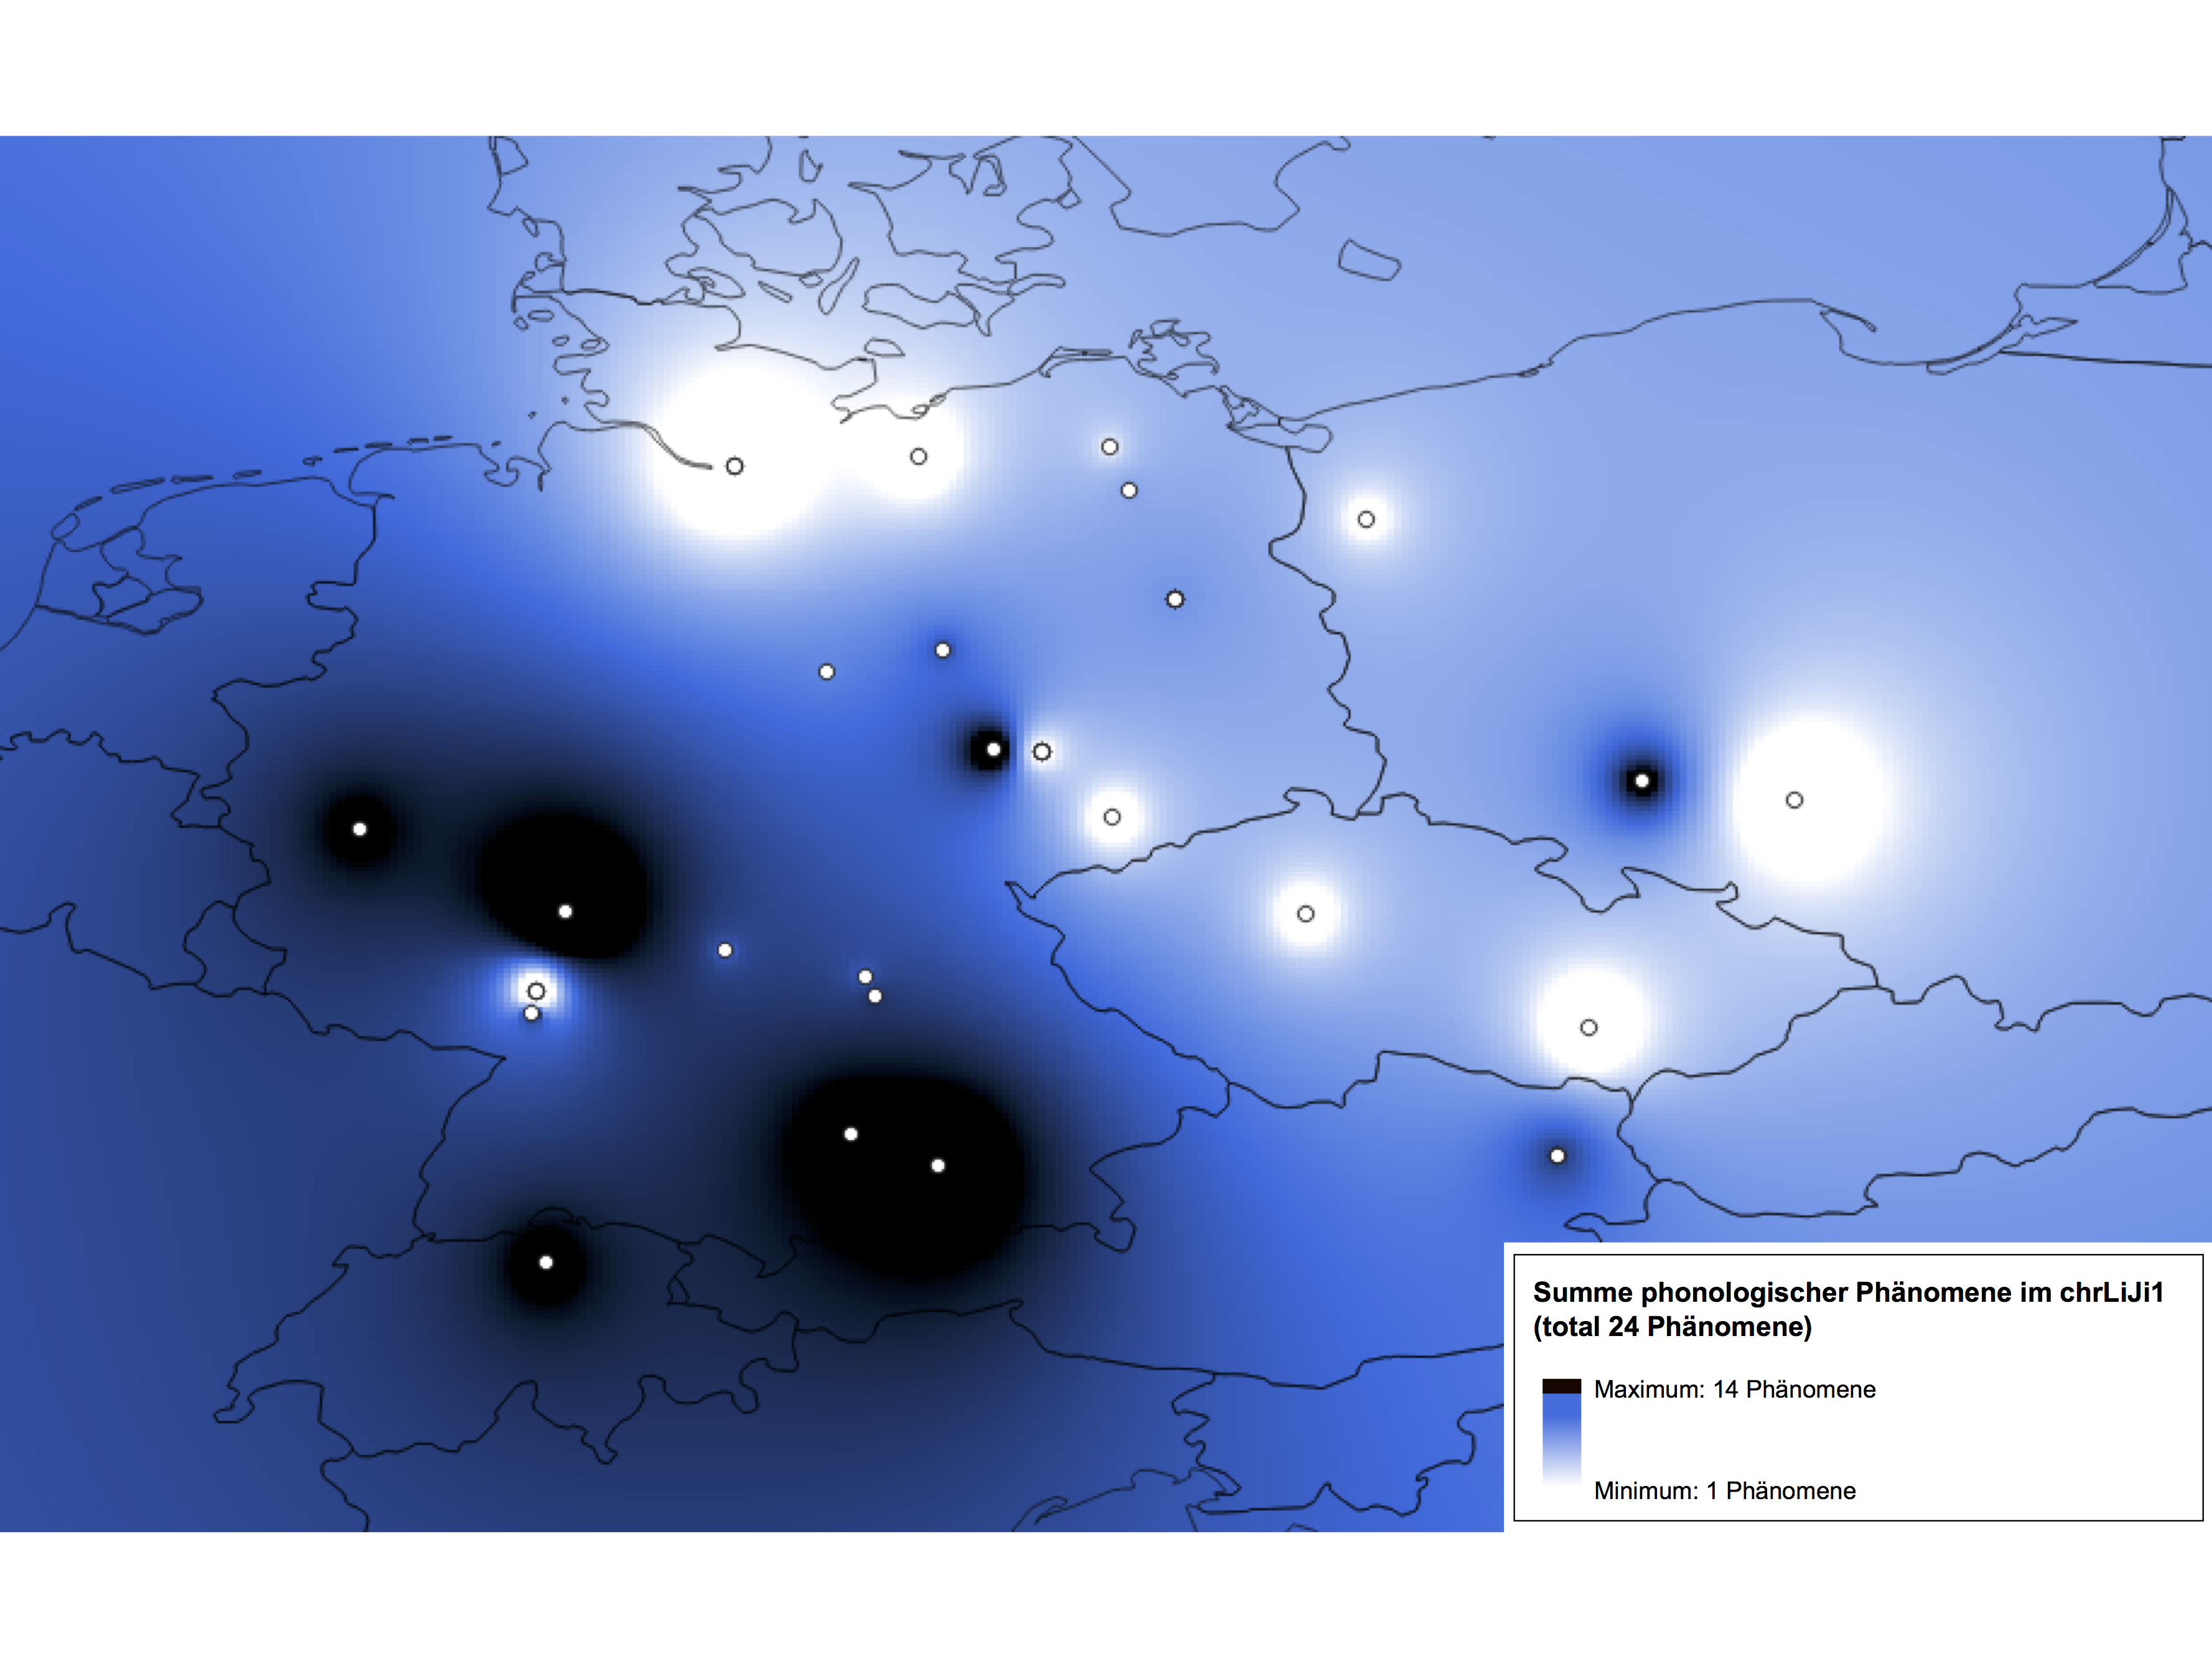
\includegraphics[height=.4\textheight]{figures/phon_IDW_legende.png}
		\caption{\label{kartelijiIDWQGIS} Summe phonologischer Phänomene im \hai{chrLiJi1} (\hai{IDW} berechnet mit \hai{QGIS})}
		\end{figure}
		

 
  Die Karte in Abbildung \ref{lijiphon} fasst die Summe zusammen, wie viele phonologische Phänomene (von 24 analysierten Phänomenen)\footnote{Um eine Vergleichbarkeit mit der Situation in den deutschen Dialekten zu gewährleisten (s.\,u.), wurden lediglich Phänomene aufgenommen, zu denen vergleichbare Informationen aus den Dialekten gegeben waren. Diese 24 Phänomene sind: die westjiddische Monophthongierung und der \isi{Zusammenfall} von \hai{V24} und \hai{V44}, die westjiddische Diphthongierung von \hai{V42}, \hai{V22}, \hai{V34} (< {\mhd} \textit{iu}), die \textit{a}-Verdumpfung, \,%rs kursiv
 Wechsel von /o/ > /u/ und /u/ > /o/, die \isi{Palatalisierung} von /u/ > /y/, die vier Möglichkeiten der \isi{Entrundung} von /y/ und /oe/, die \isi{Koronalisierung} im An- und \isi{Auslaut}, die Lenisierungen von /ts/ > /s/, /z/ und von /t/ > /d/ und /p/ > /b/, sowie die Fortisierungen von /b/ > /p/ und /g/ > /k/, der Erhalt von {\westgerm} -\textit{pp}- und die Spirantisierung von /b/ > /v/.} eine Quelle verwendet. Für Orte, an denen mehr als eine Quelle vorliegt, wurde der Mittelwert aller Quellen berechnet und ist als solcher in die Kartierung eingegangen. Man sieht so, dass besonders wenige Markierungen im nördlichen und östlichen Teil des Untersuchungsgebiets auftreten. Im Zentrum, Süden und äußeren Westen hingegen findet sich eine größere Vielfalt an phonologischer Markierung. Besonders die Frankfurter Quellen und die eine belegte Münchner Quelle betreiben einen besonders hohen Aufwand bei der phonologischen Manipulation. Der generelle Durchschnitt (Mittelwert) der hier kartierten 24 Phänomene beträgt, bei einer relativ hohen Standardabweichung von {$\sigma$}\,3,38, im \hai{chrLiJi1} 6,45 Phänomene pro Ort.


\newpage 	 
Für die Karte in Abbildung \,%rs die Karte in Abbildung
\ref{kartelijiIDW} wurden die Daten aus der Karte in Abbildung \,%rs  aus der Karte in Abbildung
 \ref{lijiphon} mittels inverser Distanzwichtung (Inverse Distance Weighting, kurz \hai{IDW}) interpoliert.\footnote{Die \hai{IDW} wurde hier nach der im Spatial Analyst Modul des Kartierungsprogramms \hai{ArcGIS 10.1} (ESRI Inc.) und/oder des entsprechenden Tools des Karierungsprogramms \hai{QGIS} (Version 2.4 \textit{Chugiak}) festgelegten Formel berechnet und wie alle Karten dieser Arbeit mit eben diesem Programm erstellt. Dabei werden zunächst, wie bei jeder Form von Interpolation, die gegebenen Datenwerte  \hai{Z\textsubscript{1}}, ...,  \hai{Z\textsubscript{n}}, \,%rs ,
 die mit unterschiedlichen Orten verknüpft sind \hai{P\textsubscript{1}}, ..., \hai{P\textsubscript{n}}, \,%rs ,
 miteinander in Beziehung gestellt. Der interpolierte Wert ist ein gewichteter Durchschnitt aller Datenwerte. Die \textit{Abweichungen} (\textit{Schwere}, \textit{weights}) der einzelnen Datenpunkte zu diesem Durchschnitt ist \hai{w}. Um den tatsächlichen Mittelwert zu ermitteln muss durch die Summe aller \textit{Abweichungen} geteilt werden: 
\begin{math} 
Z = \frac{[w\textsubscript{1} \cdot Z\textsubscript{1} + ... + w\textsubscript{n} \cdot Z\textsubscript{n}]}  {[w\textsubscript{1} + ... + w\textsubscript{n}]}
\end{math}%
. Bei einer \hai{IDW} wird der Grad der \textit{Abweichung} durch den Wert \hai{p} beeinflusst. Dieser gewährleistet dass die Abweichungen zwischen  Datenpunkt (\hai{P}) und Interpolationspunkt (\hai{P}\textsubscript{i}) proportional verlaufen: 
\begin{math} w\textsubscript{i} = \frac{1} {\text{Abstand}\,(P, P\textsubscript{i})^p} \end{math} . Für \hai{p} wurde der Wert \hai{p}=2 gesetzt. Der Zahlenwert selbst spielt nur eine geringe Rolle;\, zentral ist, dass alle \hai{P}-Werte durch einen gemeinsamen \hai{p}-Wert normalisiert sind (vgl.\, \citealt[132–160]{BurroughMcDonnell1998}).} Dies ermöglicht eine bessere räumliche Darstellung. Damit erkennt man deutlich, dass das \hai{chrLiJi1} besonders vielfältig phonologische Manipulationen einsetzt und sich ein gewisser Grad der Abnahme gegen Nordosten ergibt. 
  






 \begin{figure}[p]
		 
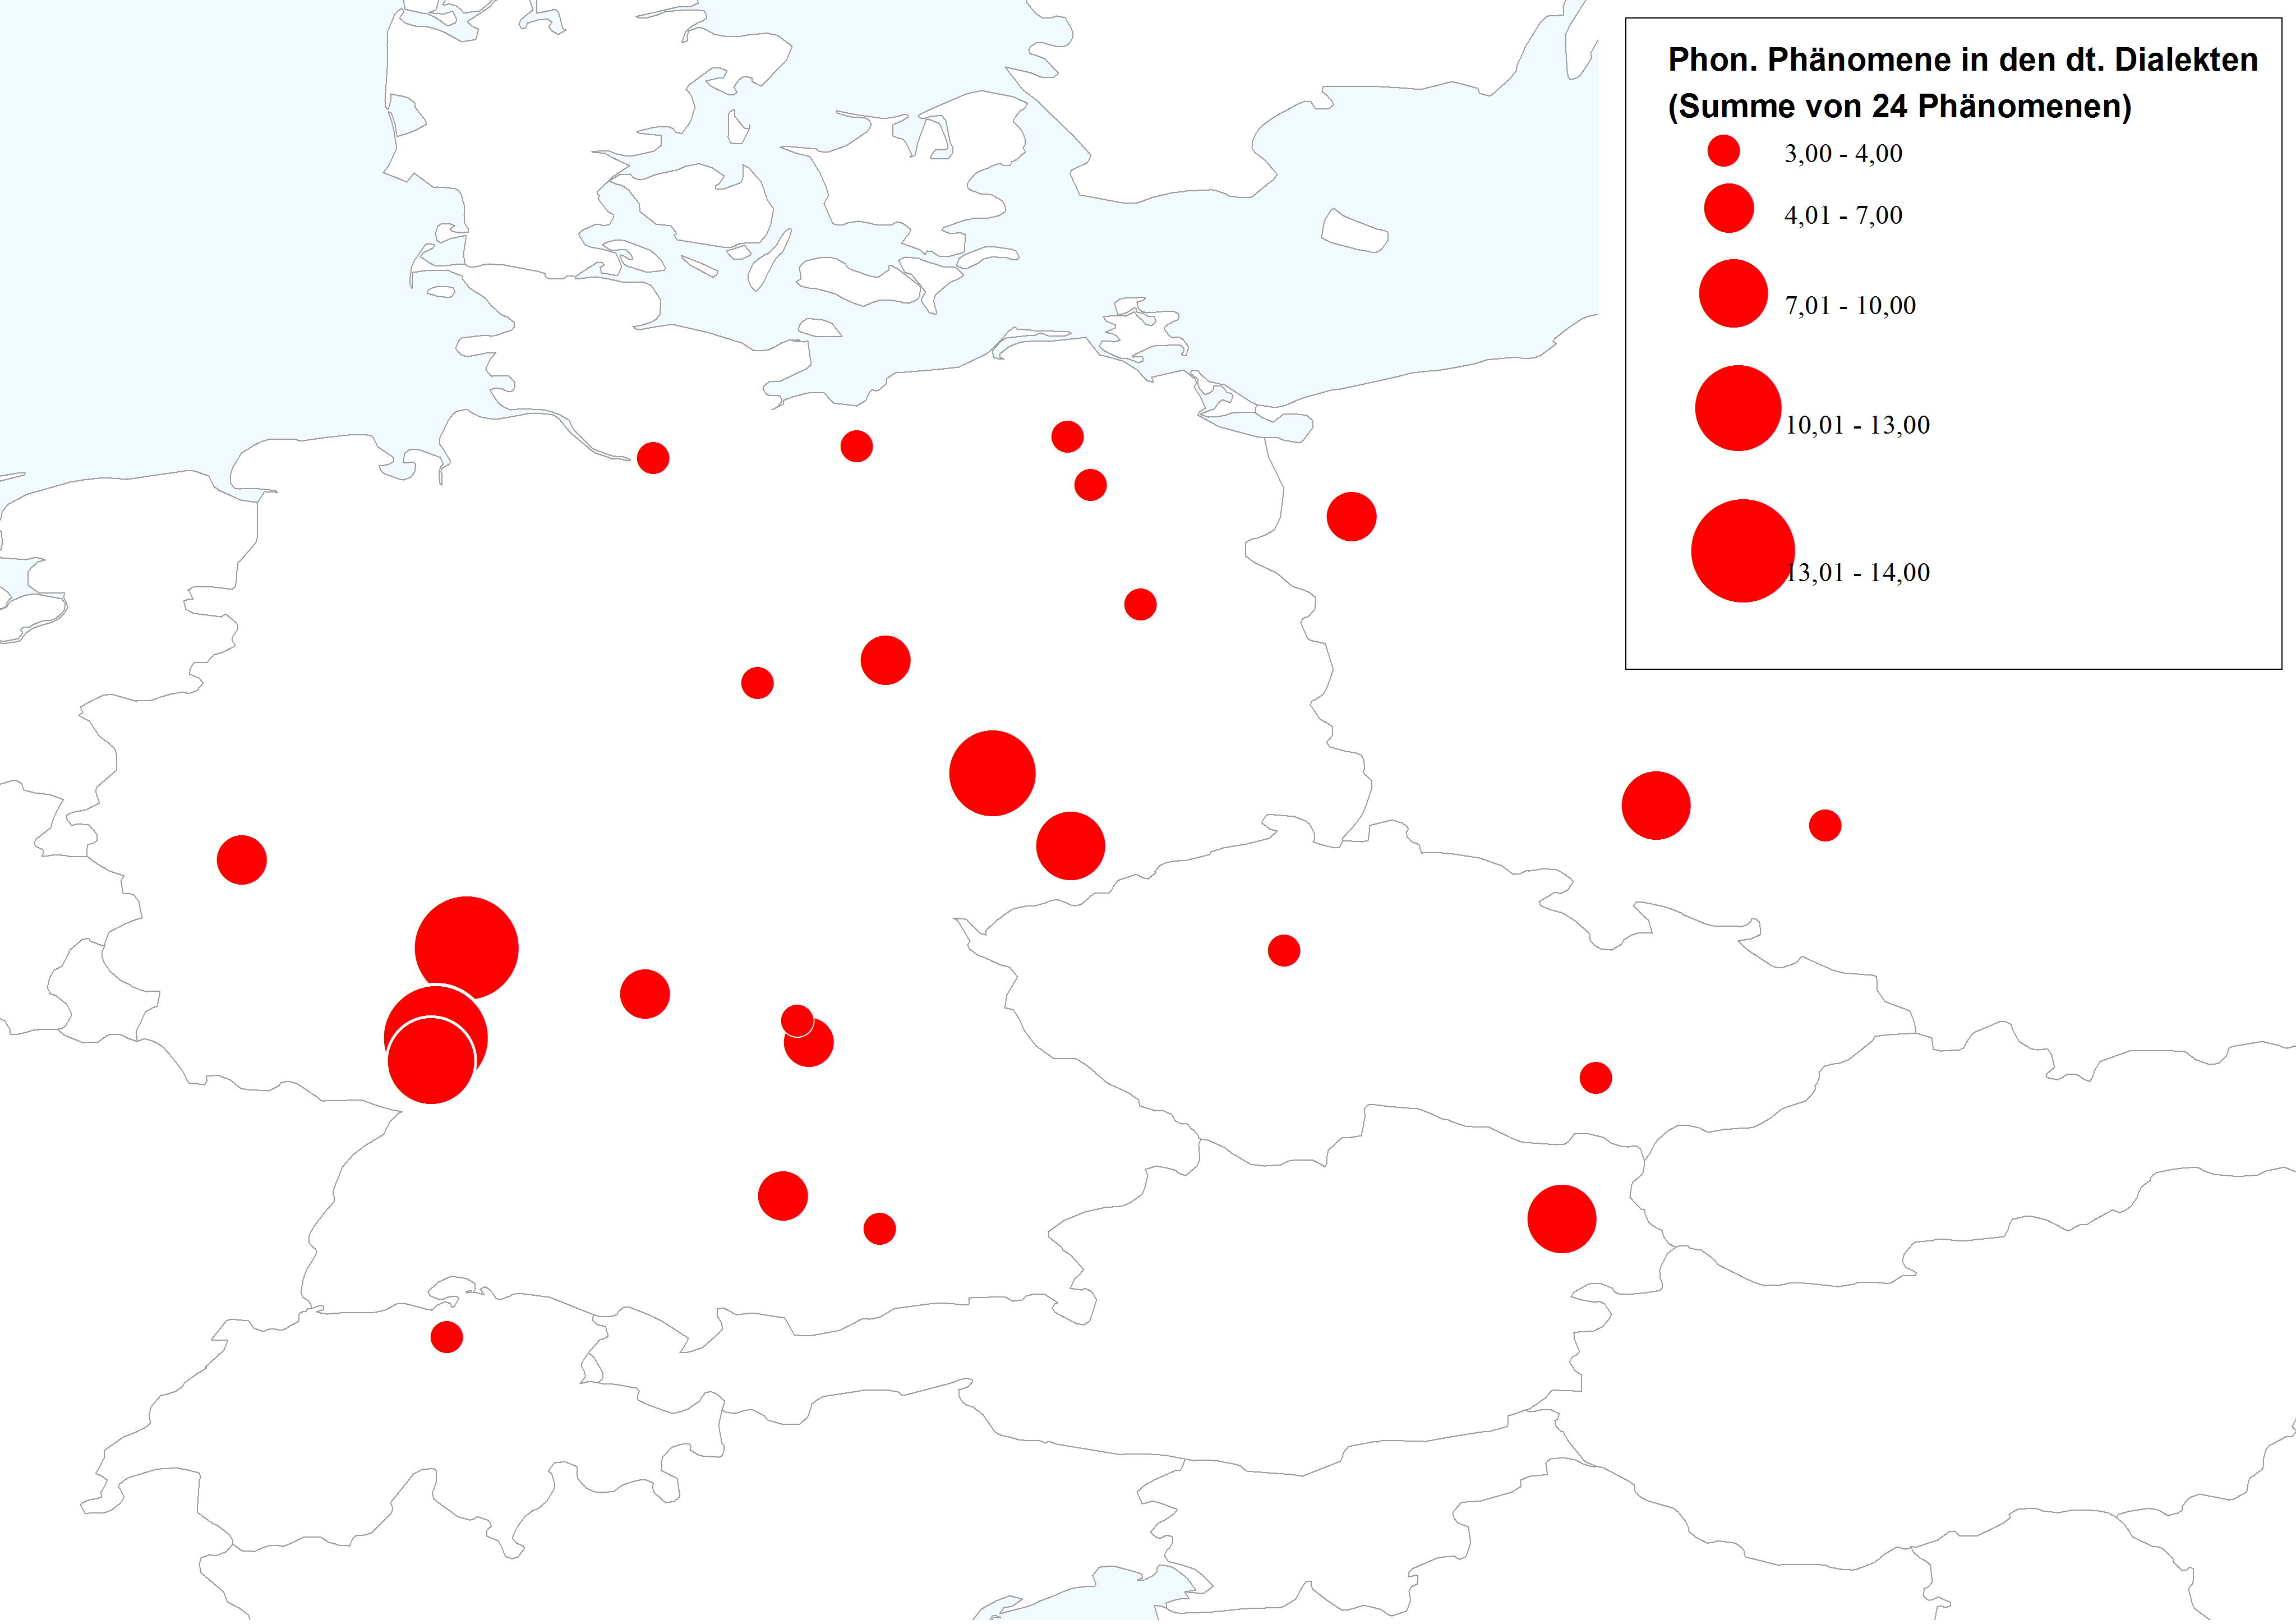
\includegraphics[height=0.4\textheight]{figures/phon_dt_dialekte.png}
		\caption{\label{allphondt} Summe phonologischer Phänomene des \hai{chrLiJi1} in den entsprechenden dt. Dialekten}
		\end{figure}
		
		
\begin{figure}[p]
		 
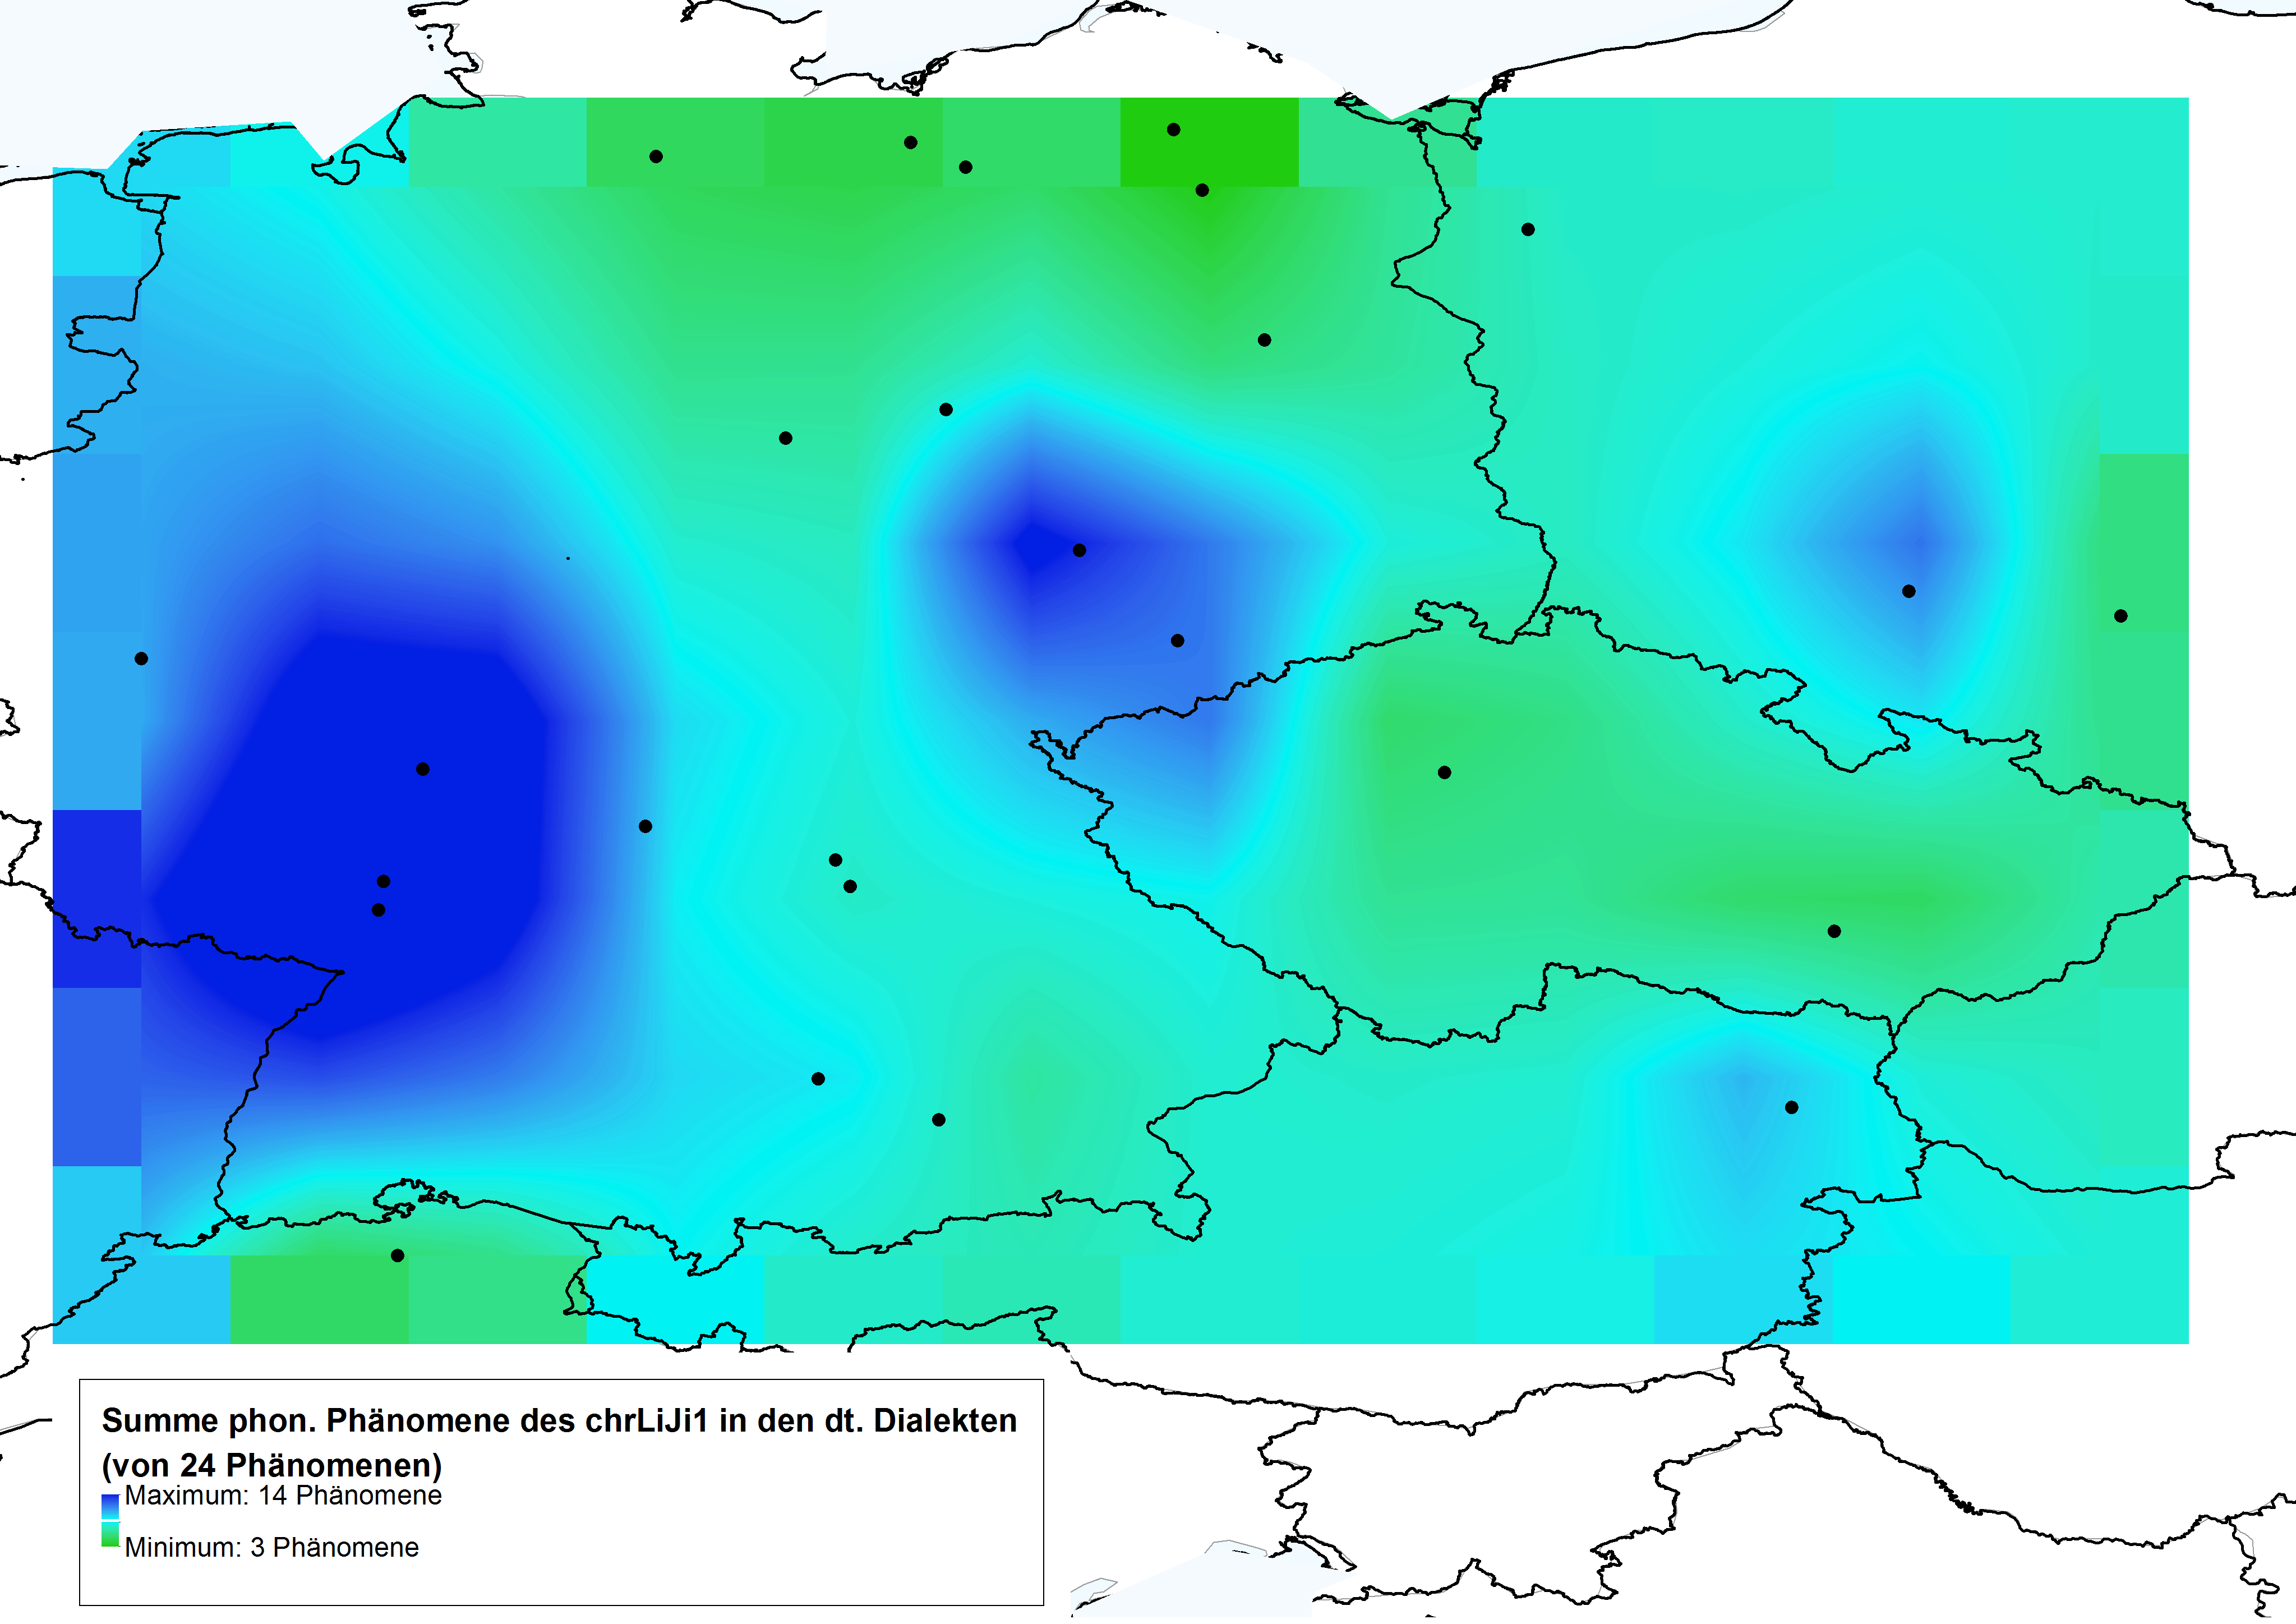
\includegraphics[height=0.4\textheight]{figures/phon_dt_nurIDW_PUNKT.png}
		\caption{\label{IDWphondt} Summe phonologischer Phänomene des \hai{chrLiJi1} in den entsprechenden dt. Dialekten (\hai{IDW})}
		\end{figure}

Da ein gewisser Einfluss der örtlichen Dialekte auf das \hai{chrLiJi1} denkbar ist, wurden zu den einzelnen Orten des \hai{chrLiJi1} die entsprechenden Situationen in den deutschen Dialekten aufgenommen und, sofern diese deckungsgleich mit den phonologischen Phänomenen des \hai{chrLiJi1} \,%rs , streichen
sind, \,%rs ,
in der Karte in Abbildung \ref{allphondt} \,%rs in Abbildung
kartiert und in der  Karte in Abbildung\ref{IDWphondt} \,%rs in Abbildung
 mittels \hai{IDW} interpoliert.\footnote{Die Daten zu den deutschen Dialekten ergeben sich aus den in den Einzelanalysen herangezogenen Quellen, sprich vorwiegend den Daten des \hai{WA} u. des \hai{KDSA}.} Der Mittelwert aller deutschen Dialekte zu den Phänomenen ist mit  6,31 Phänomenen pro Ort sehr ähnlich wie im \hai{chrLiJi1};die Standardabweichung beträgt hier {$\sigma$}\,3,6. Es zeigt sich hier besonders in Mittel- und Süddeutschland (und Österreich), dass aus den deutschen Dialekten potenziell mehr Phänomene bekannt hätten sein müssen, als sie im \hai{chrLiJi1} verwendet wurden. Andere Quellen, \,%rs ,
 wie etwa im Frankfurter, Mannheimer, Augsburger und Breslauer Raum, \,%rs ,	
 zeigen eine ähnliche Anzahl an Phänomenen im \hai{chrLiJi1} wie auch in den deutschen Dialekten. Die Karte in Abbildung  \ref{allphondt} %\,%rs in Abbildung
 zeigt uns darüber hinaus, dass das \hai{{\LiJieins}} eine Vielzahl phonologischer Phänomene mit den deutschen Dialekten, \,%rs Dialekten
 insbesondere den rheinfränkischen und obersächsischen, teilt. Der Vergleich der Karten in Abbildung \ref{IDWphondt} und in Abbildung \ref{kartelijiIDW} \,%rs in Abbildung (2mal)
  zeigt, dass besonders die südöstlichen Quellen (München, Augsburg, Erlangen, Nürnberg) eine Vielzahl phonologischer Manipulationen aufweisen, die am Ortsdialekt selbst nicht vorhanden sind.



Doch diese Daten alleine zeigen nur die reine Quantität phonologischer Phänomene und noch nicht, welche Phänomene, die an einem Ort im \hai{chrLiJi1} vorliegen, auch im entsprechenden deutschen Dialekt belegt sind. Die genaue Schnittmenge zwischen phonologischen Phänomenen, die im \hai{chrLiJi1} an einem Ortspunkt gewählt werden und die selbst im Ortsdialekt verbreitet sind, findet sich in den Karten in Abbildung \ref{allphondtliji} und in Abbildung \ref{IDWallphondtliji} \,%rs in Abbildung (2mal)
    dargestellt. Hier sticht der rheinfränkische Raum deutlich heraus. Und auch im Schlesischen, Obersächsischen und im Mittelbairischen Wiens gibt es starke Übereinstimmungen zwischen den im \hai{chrLiJi1} verwendeten phonologischen Manipulationen, die auch im deutschen Dialekt bekannt sind. Dabei muss beachtet werden, dass dies auch die Dialekträume sind, in denen generell die im \hai{chrLiJi1} verwendeten Phänomene auftreten (vgl.\, die Karten in Abbildung \ref{allphondt} und Abbildung \ref{IDWphondt}). \,%rs in Abbildung (2mal)
    Auch dürfen diese Karten nicht so gelesen werden, dass im \hai{chrLiJi1} besonders phonologische Phänomene aus den deutschen Dialekten genutzt wurden, sondern diese Daten veranschaulichen lediglich die Nähe der eingesetzten Phänomene zum Ortsdialekt. Wie in den Einzelanalysen gezeigt werden konnte, sind alle bisher behandelten Phänomene mehr oder weniger auf authentische jiddische Formen zurückzuführen. \hai{{\LiJieins}} ist also nicht bloß eine wahllose Zusammenschau verschiedener, in den deutschen Dialekten ohnehin weit verbreiteter Phänomene, sondern ein in sich durchaus stabiles  sprachliches System, was besonders der diachrone Blick auf die einzelnen Phänomene unterstreicht (vgl.\, Abbildung \ref{phonwjallstreu}). Die arealen Muster, die sich in den hier vorliegenden Karten erkennen lassen, sind besonders dem Umstand geschuldet, dass die (west-)jiddische Phonologie viele Eigenschaften mit den mitteldeutschen Mundarten teilt.


 \begin{figure}

		\centering
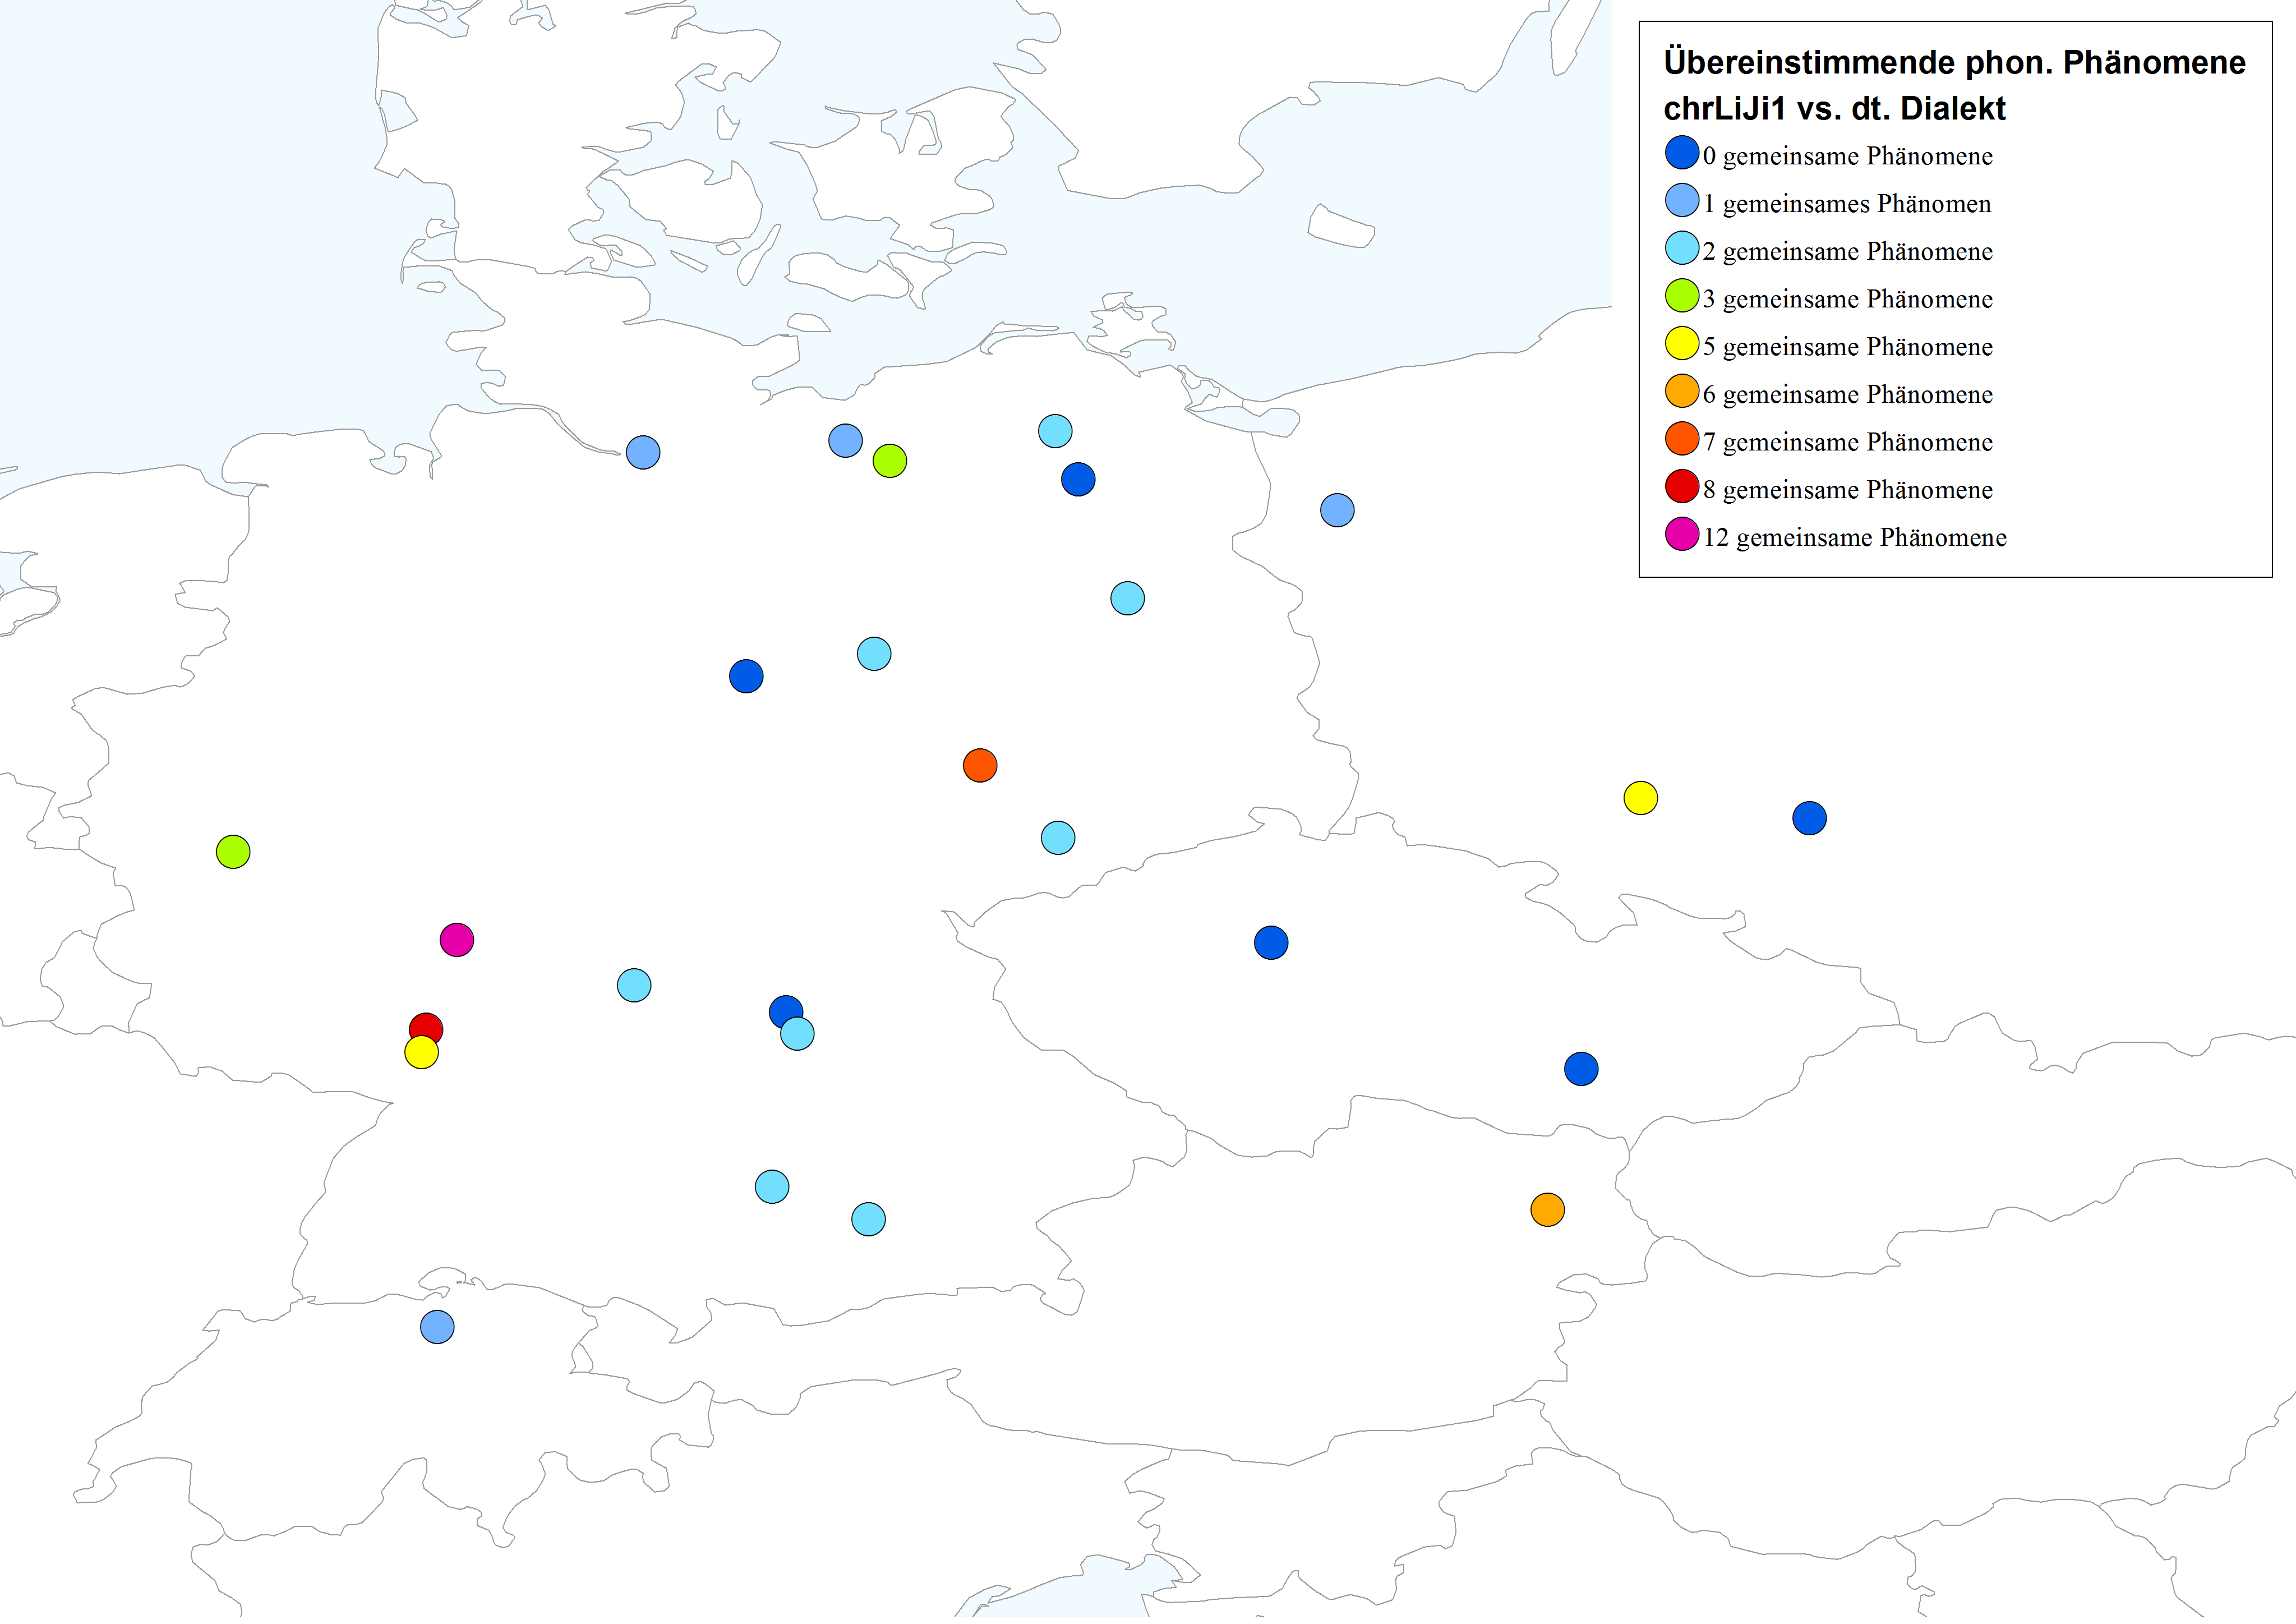
\includegraphics[height=0.4\textheight]{figures/Uebereinstimmung_phon_liji_dt.png}
		\caption{\label{allphondtliji}Gemeinsame phonologische Phänomene des \hai{chrLiJi1} und der entsprechenden dt. Dialekte}
		\end{figure}
 
 
 
 \begin{figure}
  \farbgrafik
		\centering
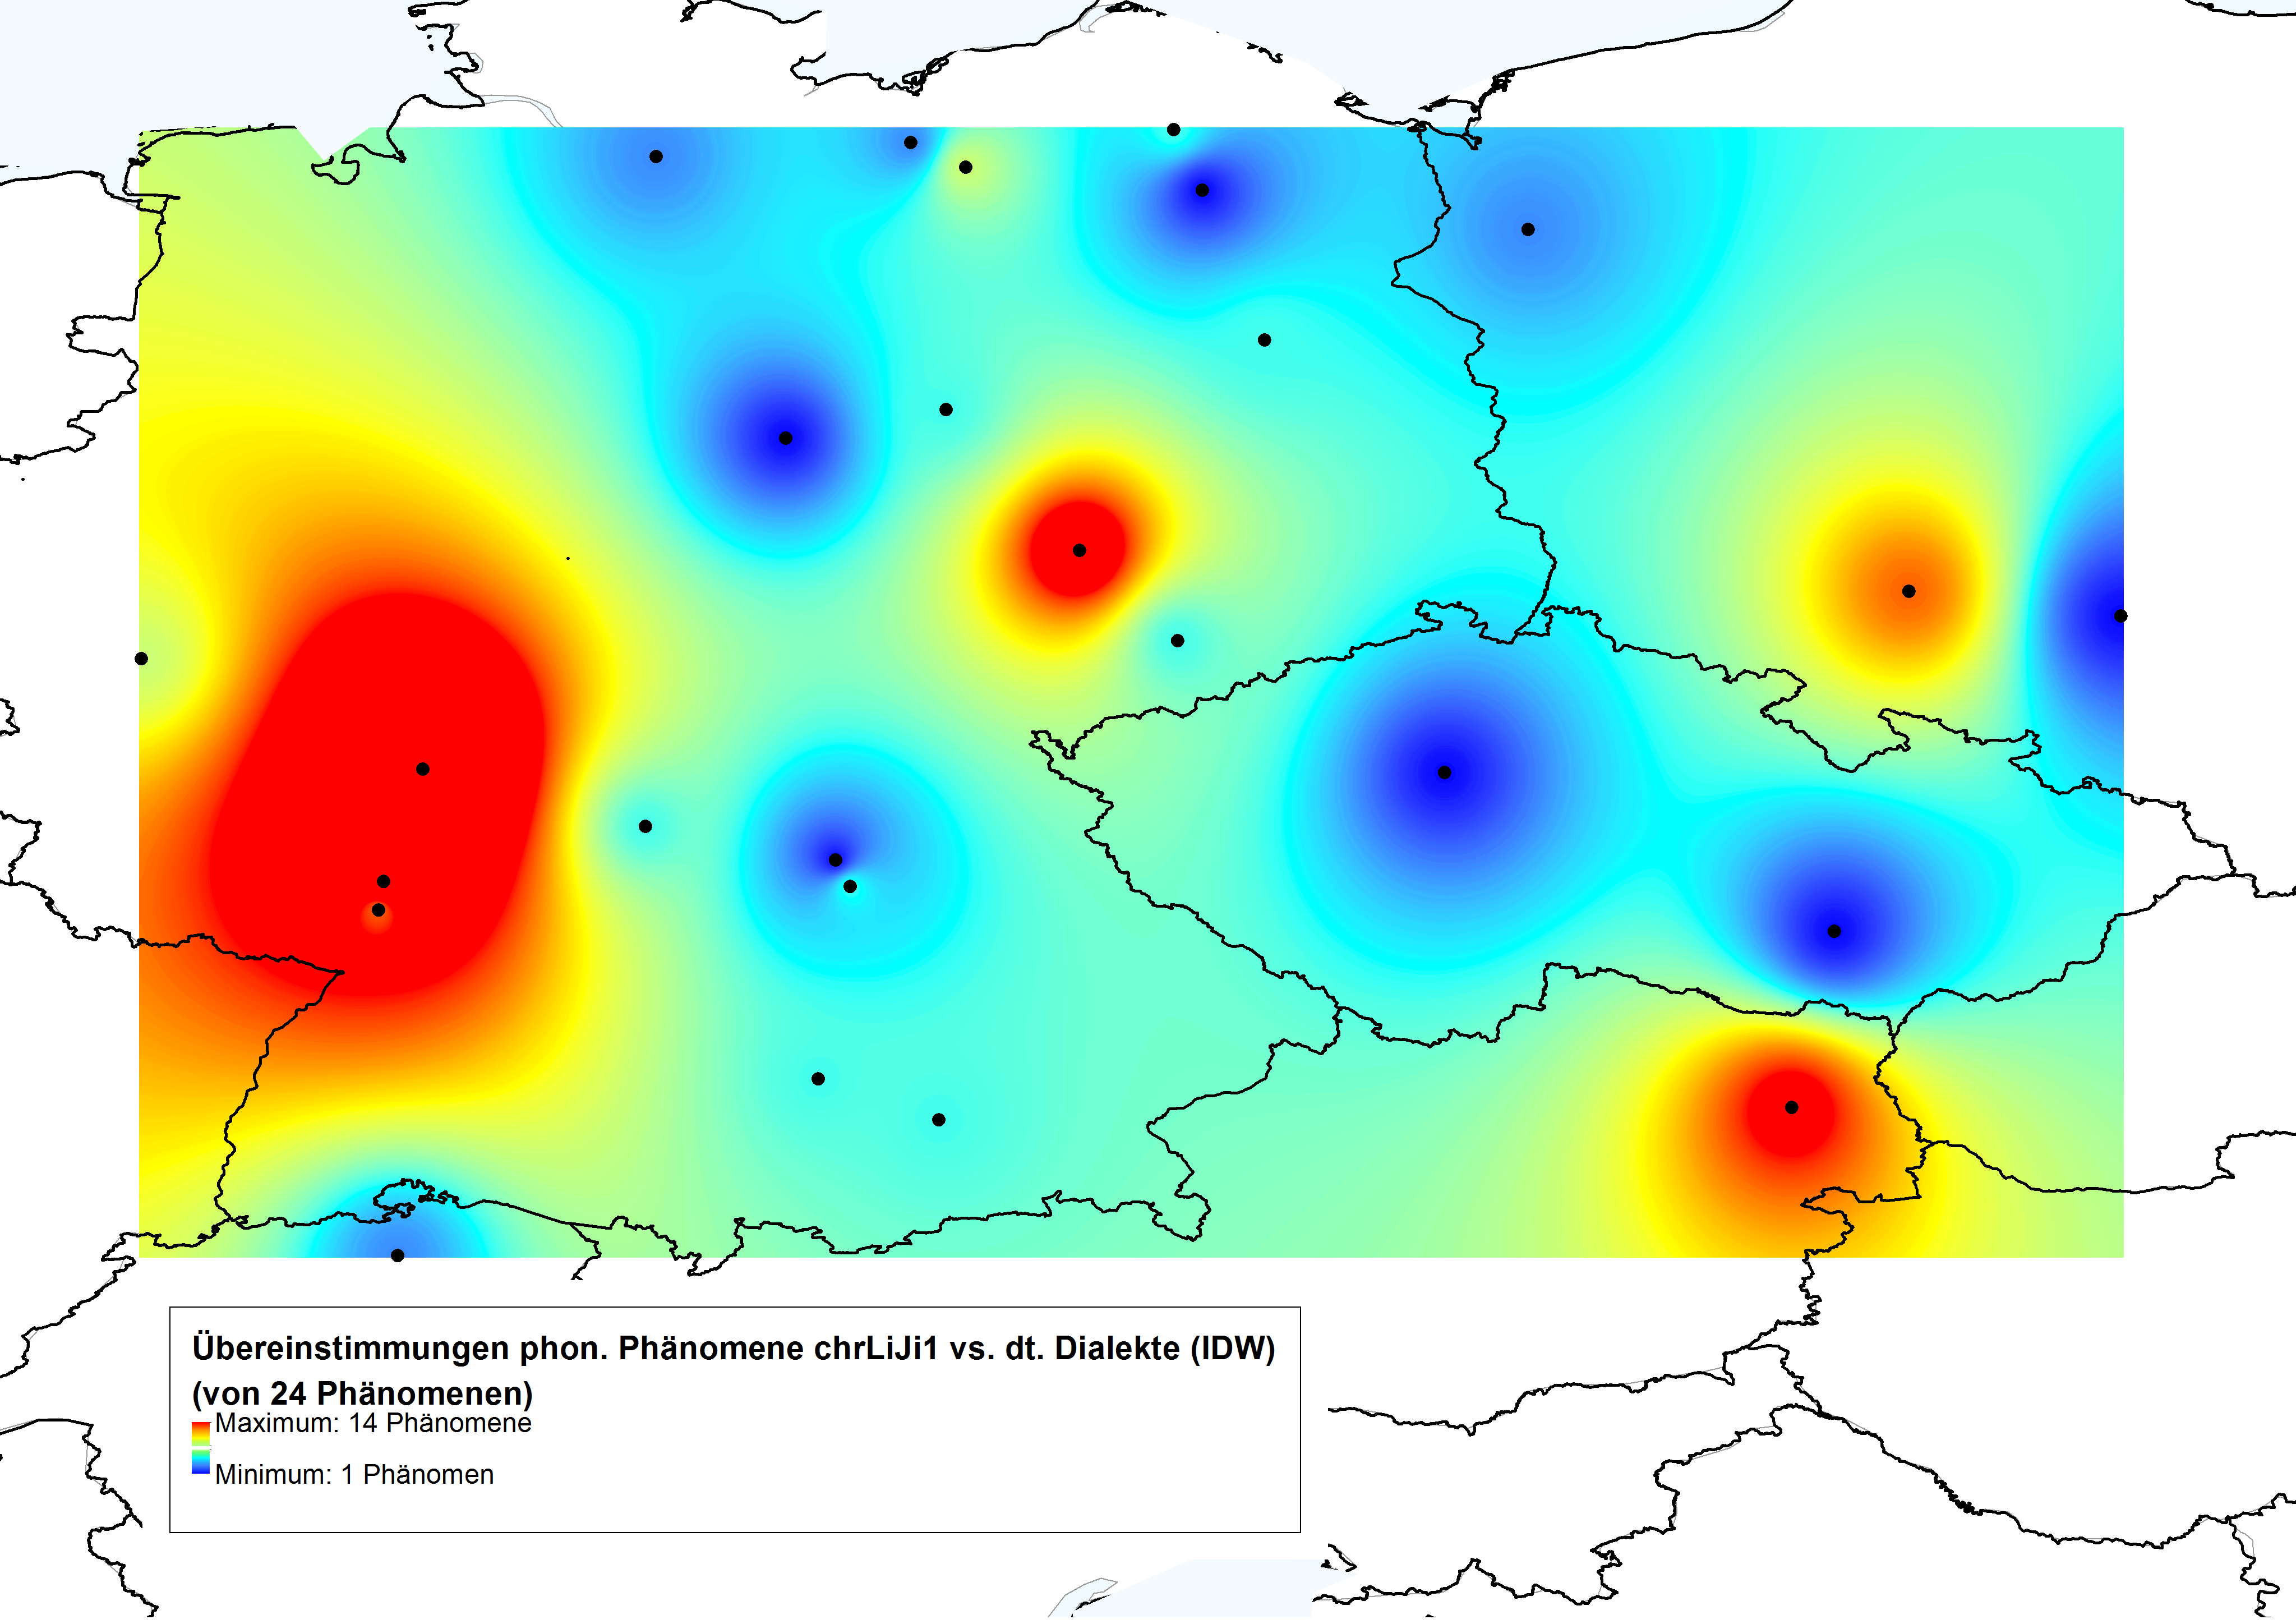
\includegraphics[height=0.4\textheight]{figures/Uebereinstimmung_phon_liji_dnurIDW_PUNKT.png}
		\caption{\label{IDWallphondtliji} Gemeinsame phonologische Phänomene des \hai{chrLiJi1} und der entsprechenden dt. Dialekte (\hai{IDW})}
		\end{figure}

  
  
 Die Karte in Abbildung \ref{allphonnegIDW} \,%rs in Abbildung
  stellt hingegen dar, wo besonders viele bzw. wenige phonologische Markierungen im \hai{chrLiJi1} auftreten, die im Ortsdialekt nicht gegeben sind. Die Differenz zwischen deutschem Dialekt und \hai{chrLiJi1} ist v.\,a.\, im Mittelbairischen und Berliner Raum besonders groß.\, Aber auch im Ripuarischen Bonns und im Mittelbairischen Wiens werden viele ortsfremde Phänomene verwendet.\,  Weniger auffällig sind die Unterschiede zwischen \hai{chrLiJi1} und deutschem Dialekt im schlesischen,\, böhmischen,\, ostpommerschen,\, alemannischen und rheinfränkischen Raum.
 

 \begin{figure} 
  \farbgrafik
		\centering
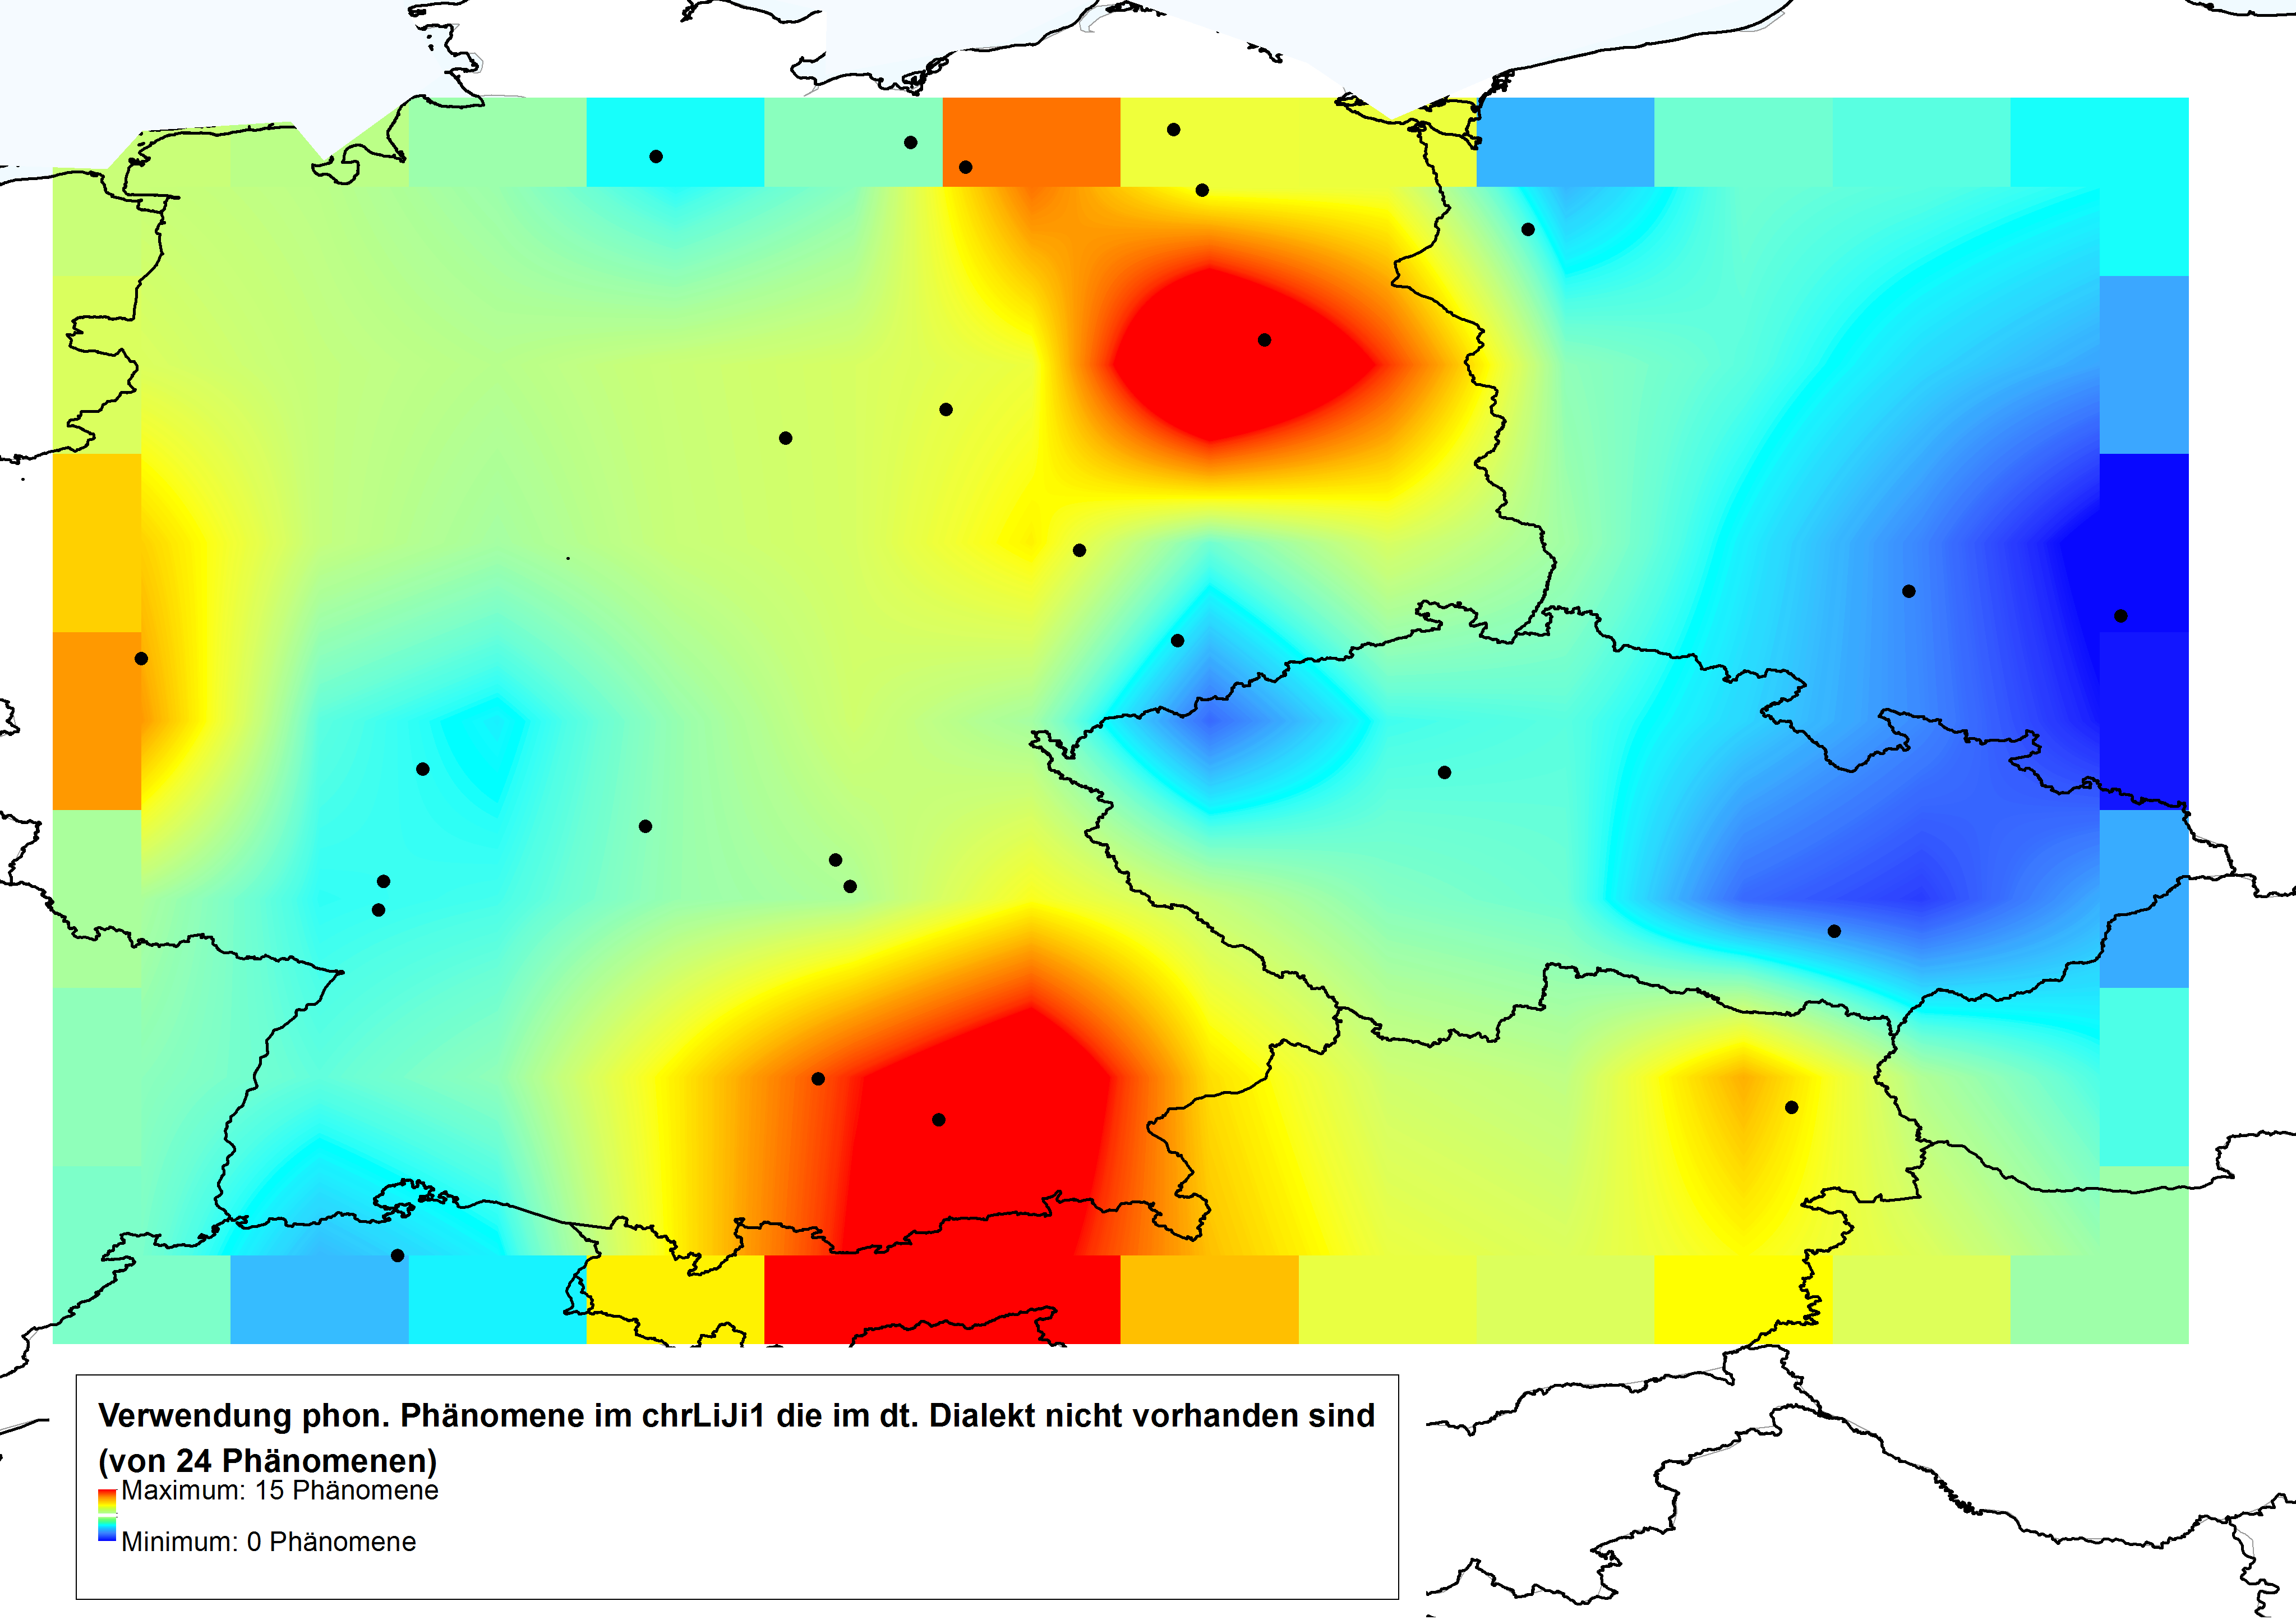
\includegraphics[height=0.4\textheight]{figures/IDW_phon_negativ_dt_liji_PUNKT.png}
		\caption{\label{allphonnegIDW} Ortsfremde phonologische Phänomene des \hai{chrLiJi1} (\hai{IDW})}
		\end{figure}

   
 Aus den Belegdaten zu sieben Phänomenen, die als besonders charakteristisch für das Westjiddische angesehen werden,\footnote{Diese Phänomene sind die Monophthongierung von \hai{V24}, \hai{V44} und deren \isi{Zusammenfall}, die Diphthongierungen von \hai{V22}, \hai{V42} und \hai{V34} sowie der Erhalt von {\germ} -\textit{pp}-.} ist die Karte in Abbildung \ref{westjiddischphonIDW} %rs Abbildung abkürzen wie sonst auch
 entstanden. Man sieht in der \hai{IDW} deutlich, dass westjiddische Formen besonders stark in den Bonner Quellen, den Texten aus den bairischen und obersächsischen Dialekträumen \,%rs Dialekträumen
  sowie denen aus Berlin auftreten;\, seltener aber im Niederdeutschen, Schlesischen, Böhmischen, Mährischen, Südbairischen, sprich im äußersten Osten des Untersuchungsgebiets. Das \hai{chrLiJi1} entspricht somit erstaunlicherweise dem Gebiet des Übergangsjiddischen, wo wir bereits ostjiddische Formen annehmen dürfen. Dies gilt zwar nicht für den äußersten Norden, wo wir auf niederdeutschem Gebiet eine Zahl an Quellen finden, in denen westjiddische Formen kaum auftreten. Auffällig verhalten sich auch die rheinfränkischen Quellen (Speyer, Mannheim, Frankfurt), die nur sehr wenige der ausgewählten westjiddischen Phänomene aufweisen, und dies obwohl sie in den örtlichen deutschen Dialekten beinahe alle gegeben sind (vgl.\, Abbildung \ref{allphonnegIDWdeutsch}). Hier kann angenommen werden, dass gerade um die Distanz zum örtlichen Dialekt herzustellen, auf charakteristische westjiddische Phänomene (zugunsten anderer) verzichtet wurde. Da es sich bei den Quellen um Theaterstücke handelt, welche besonders regional für die örtlichen Theater geschrieben wurden (insbes. im Fall der Mannheimer Quellen), ist eine erkennbare Unterscheidung zwischen jüdischem und deutschem Dialekt besonders wichtig an Orten, an denen die Gemeinsamkeiten besonders stark sind.

 
  \begin{figure}[p] 
   \farbgrafik
		\centering
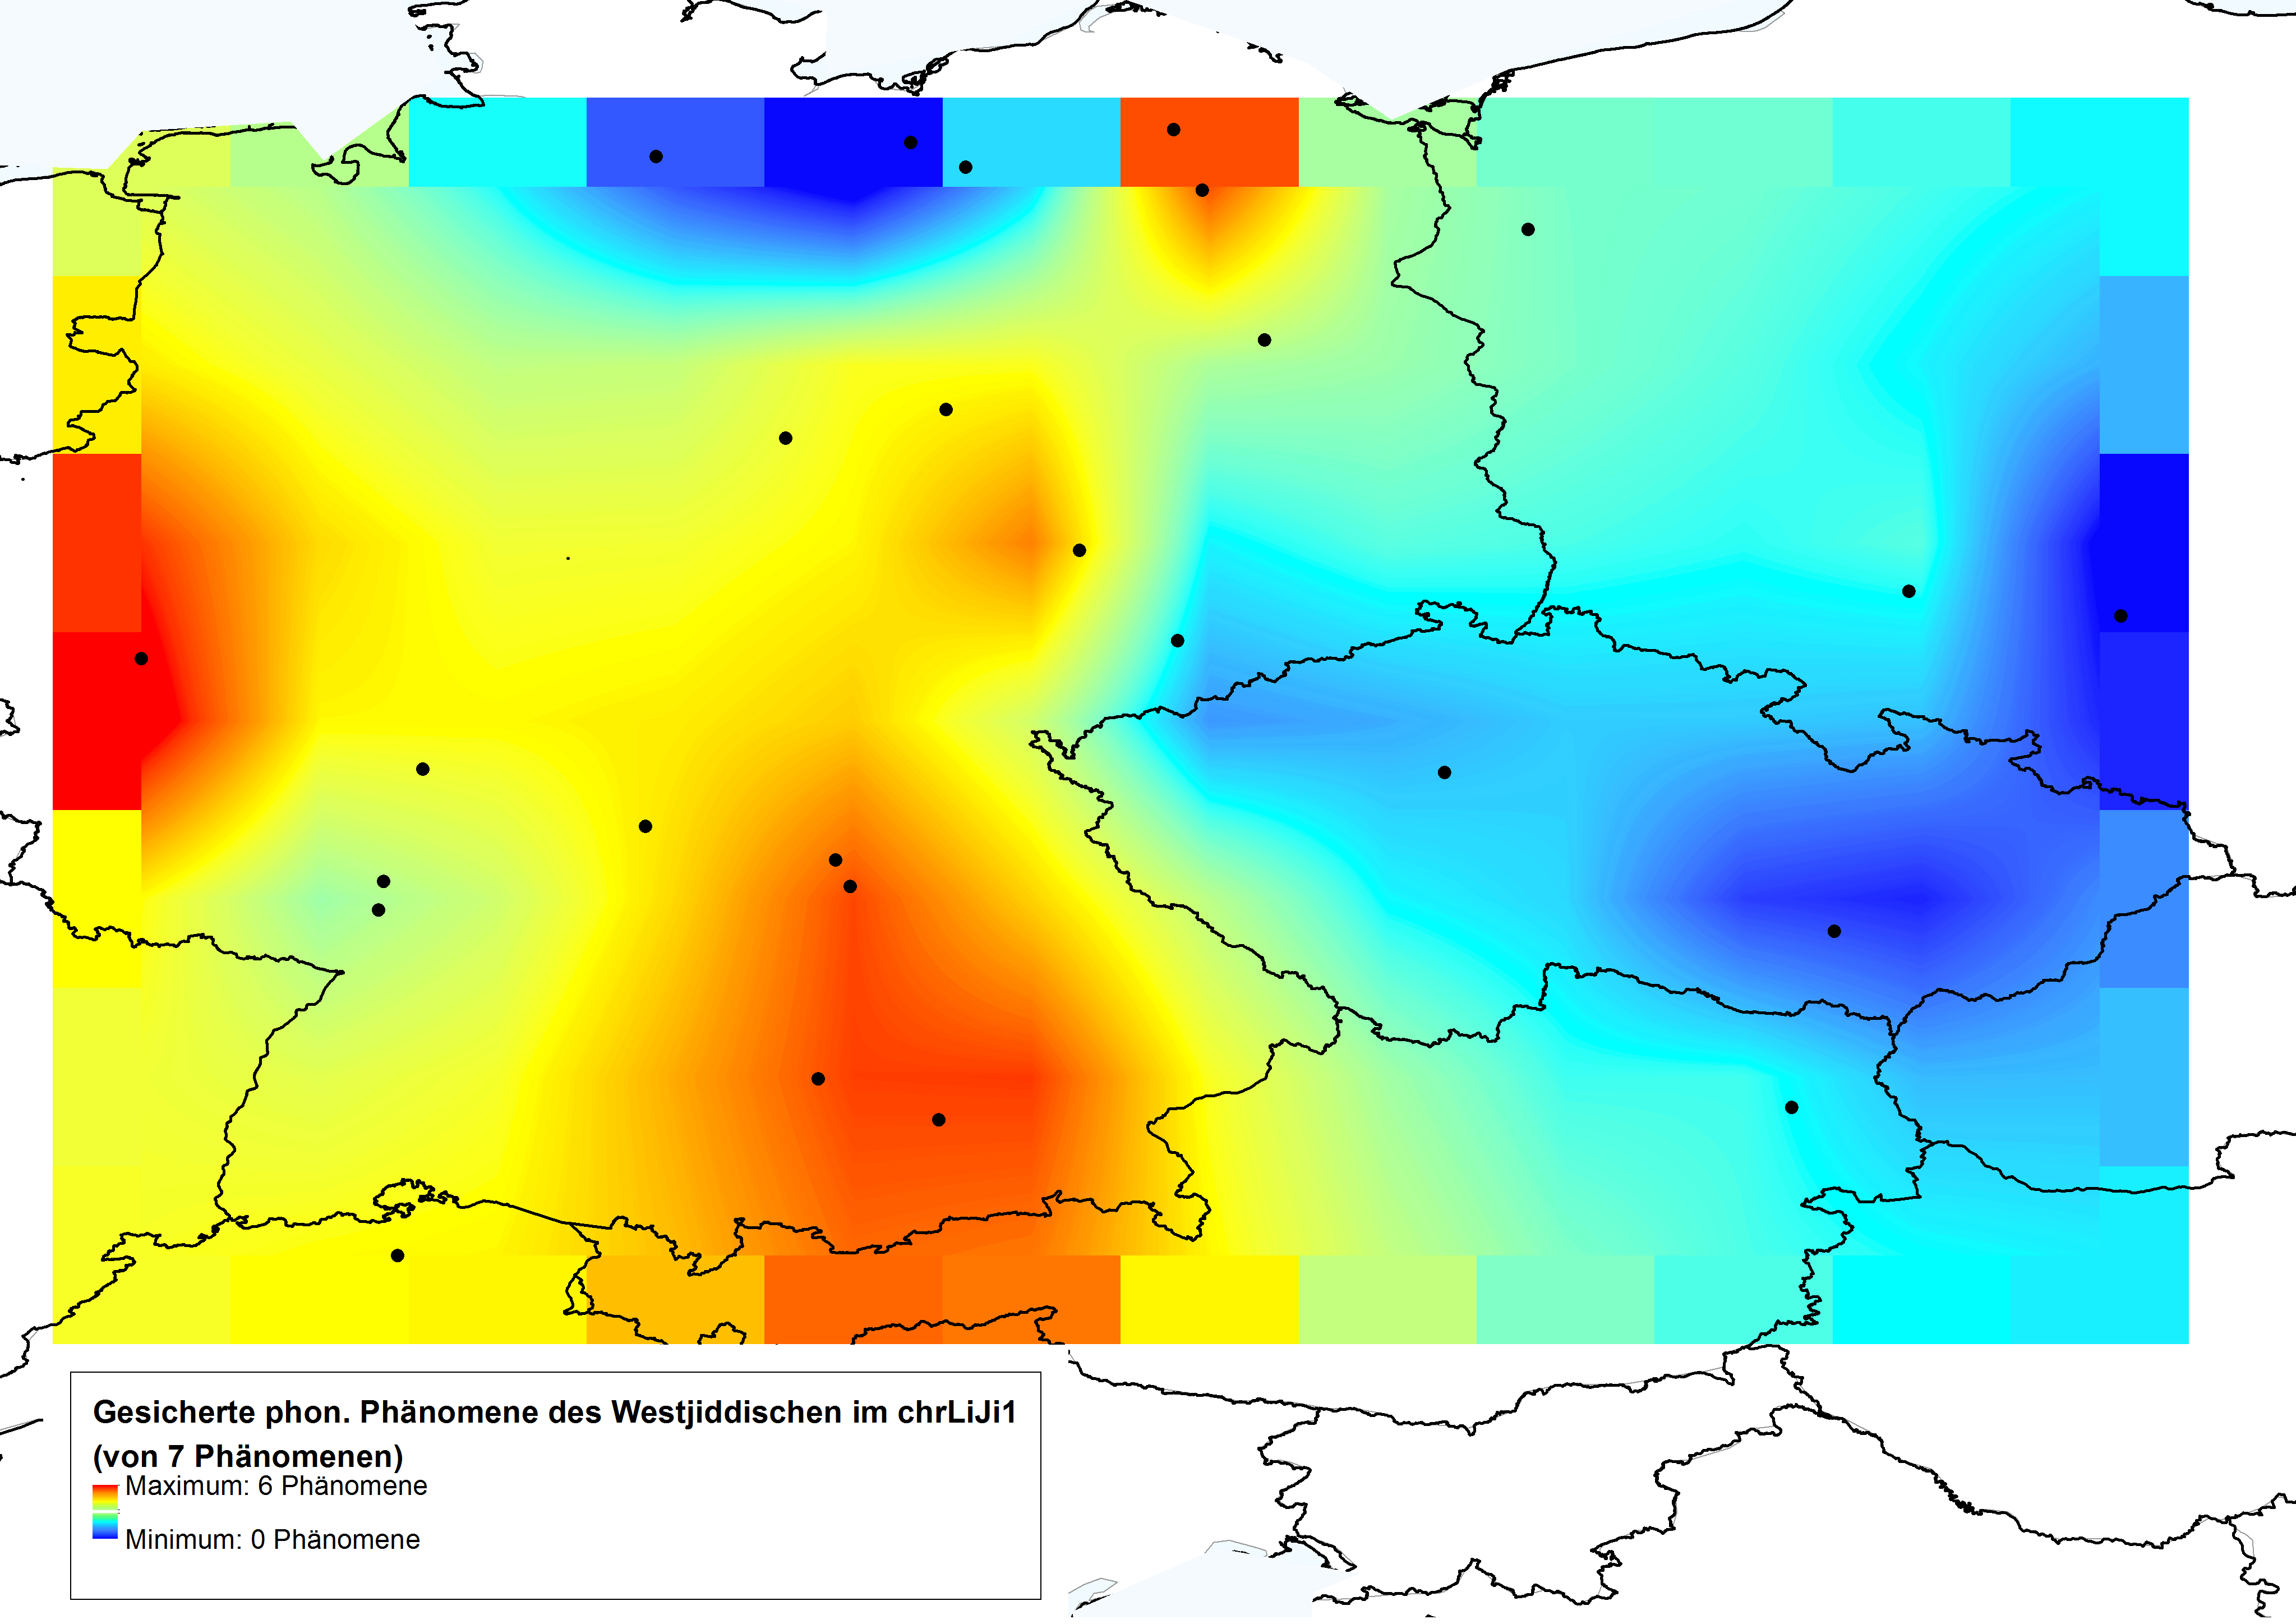
\includegraphics[height=0.4\textheight]{figures/westjiddischPHON_IDW_PUNKT.png}
		\caption{\label{westjiddischphonIDW} Westjiddische phonologische Phänomene im \hai{chrLiJi1} (\hai{IDW})}
		\end{figure}

  \begin{figure}[p]
   \farbgrafik
		\centering
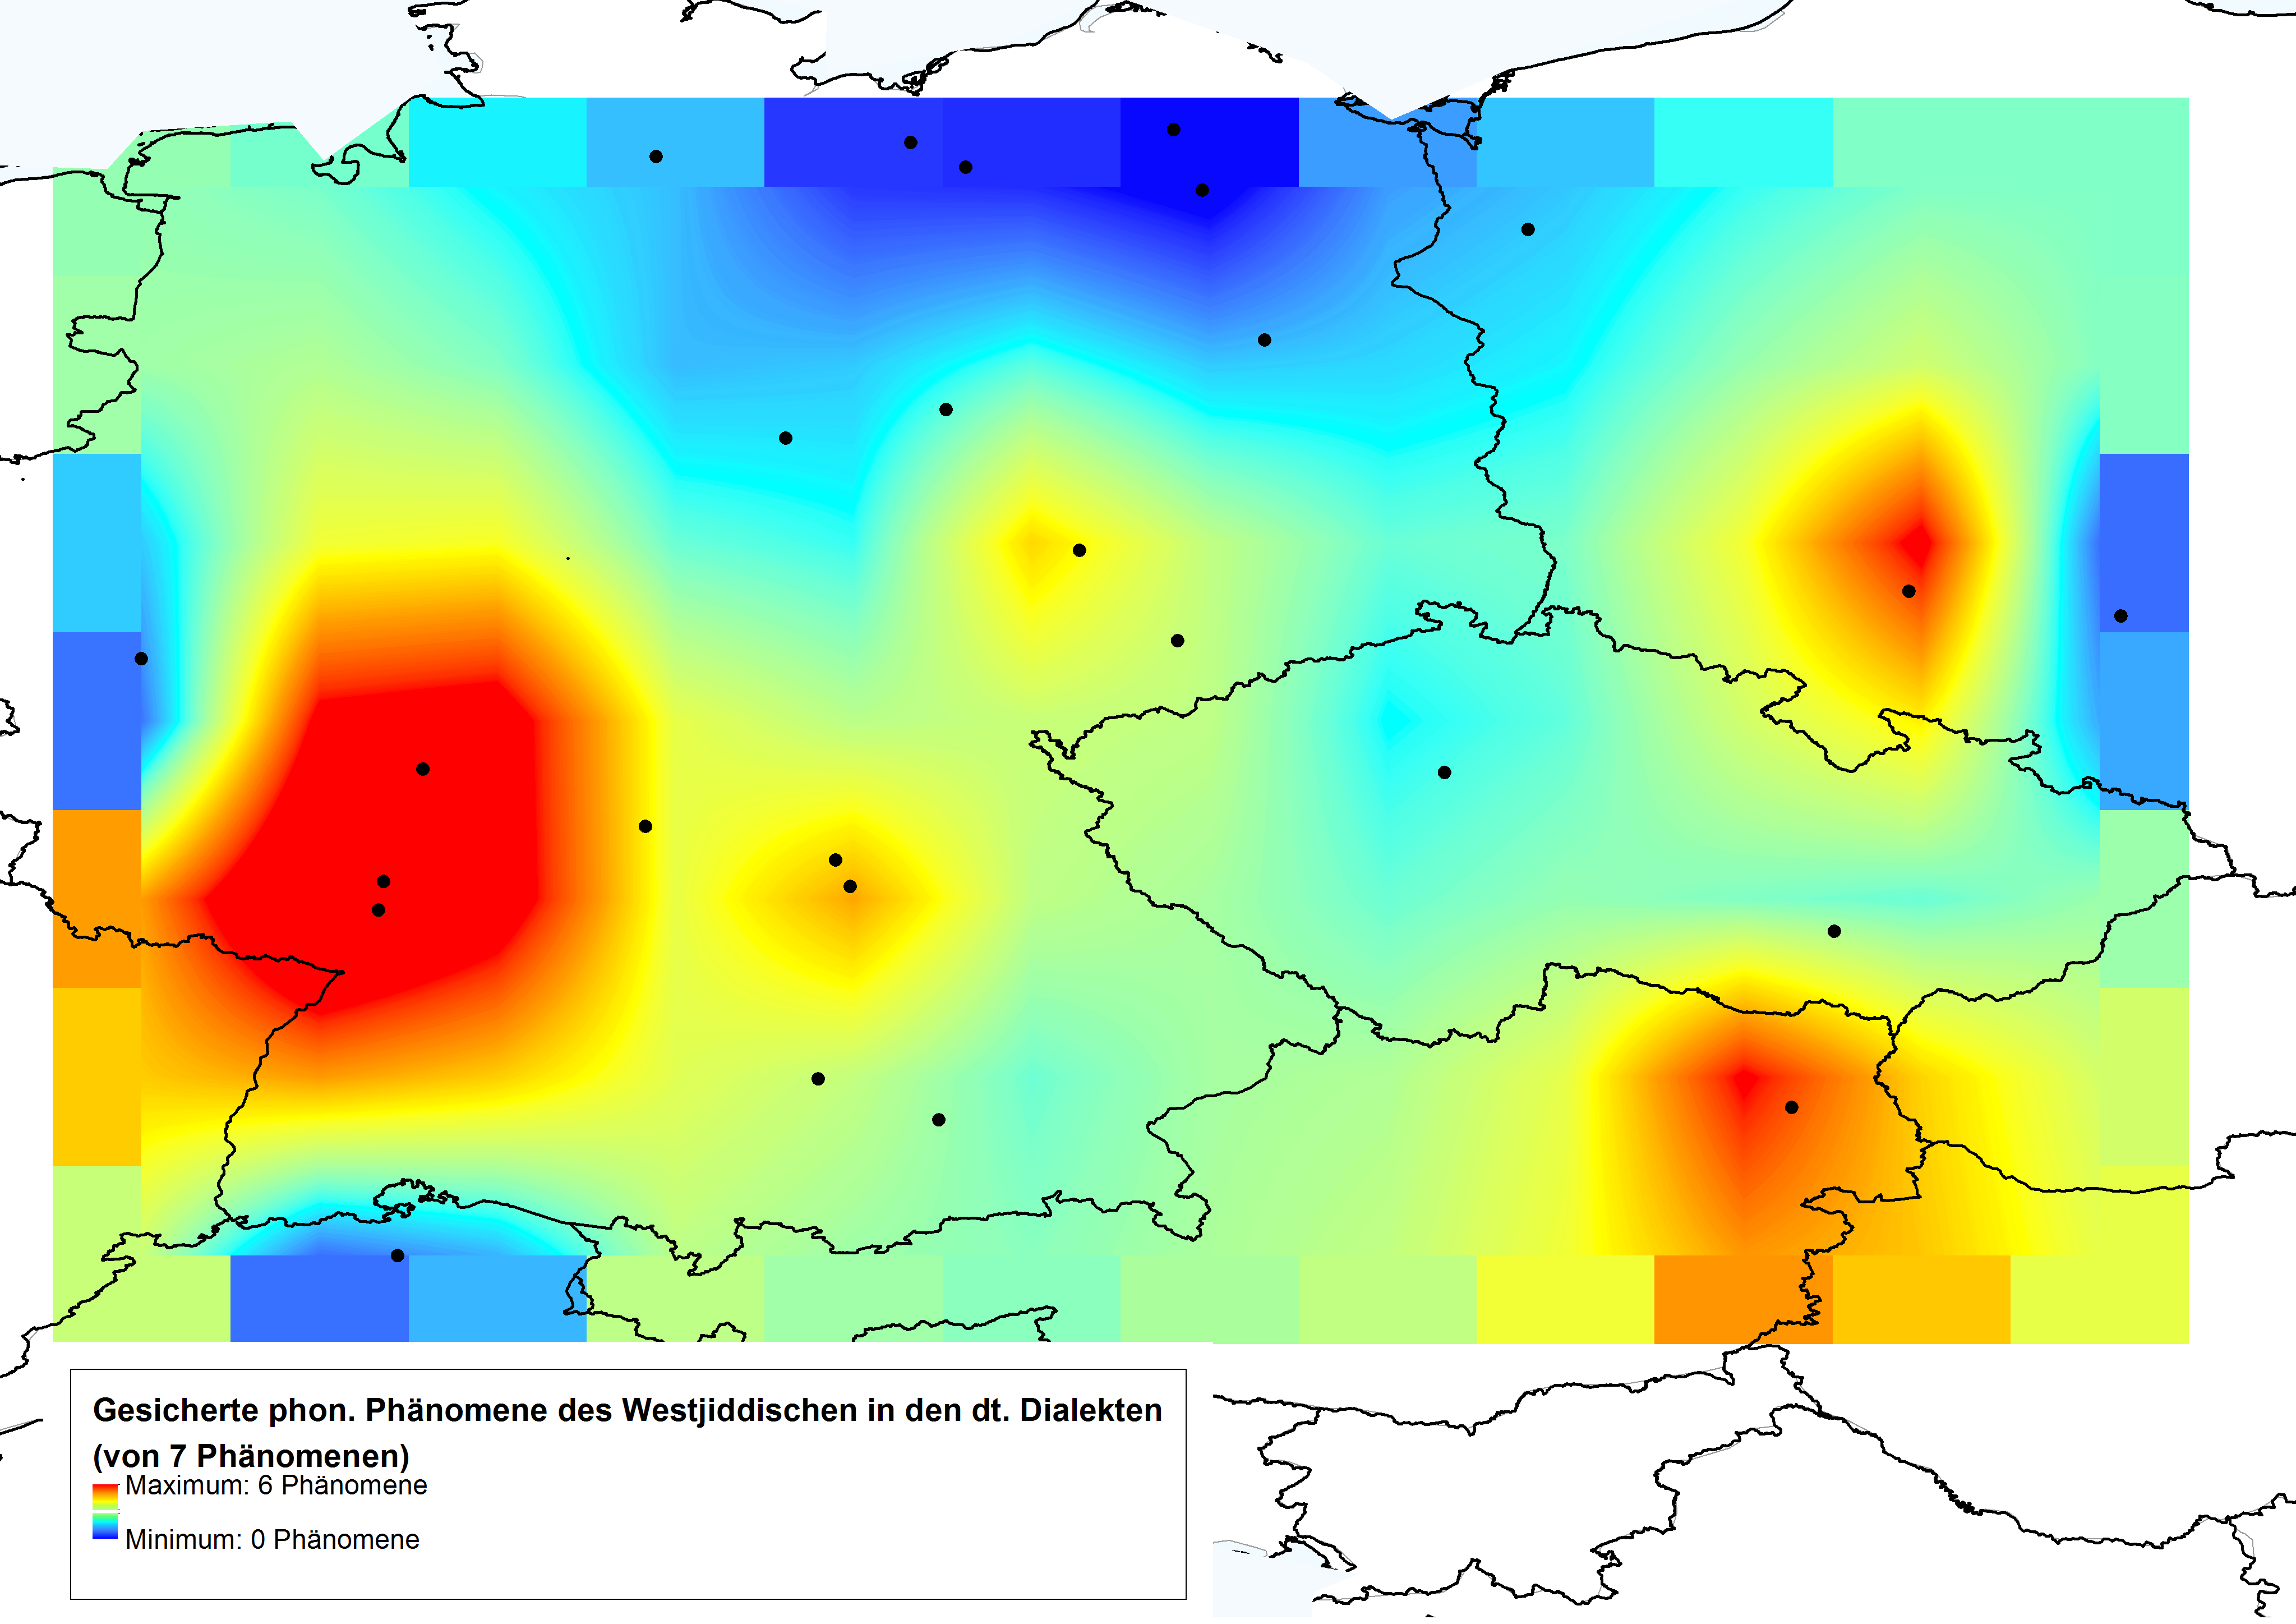
\includegraphics[height=0.4\textheight]{figures/westjiddischPHON_DEUTSCH_IDW_PUNKT.png}
		\caption{\label{allphonnegIDWdeutsch} Westjiddische phonologische Phänomene des \hai{chrLiJi1} in den dt. Dialekten (\hai{IDW})}
		\end{figure}
		 
 Das Kartenbild in Abbildung \,%rs Abbildung abkürzen wie sonst auch
 \ref{allphonnegIDWdeutsch} entspricht in etwa dem aus Abbildung \,%rs Abbildung abkürzen wie sonst auch
 \ref{IDWallphondtliji}. Hier wurden eben jene, auch für die Darstellung der Karte in Abbildung \ref{westjiddischphonIDW} \,%rs Abbildung
 relevanten, sieben besonders idiosynkratischen Phänomene des \hai{{\WJ}} herangezogen. Der Vergleich zwischen der Verteilung westjiddischer Phänomene in den deutschen Dialekten (Karte in Abbildung \ref{allphonnegIDWdeutsch}) und der Verteilung eben dieser Phänomene im \hai{chrLiJi1} (Karte in Abbildung \ref{westjiddischphonIDW}) zeigt klare Unterschiede und bestätigt damit, dass die deutschen Dialekte nur sehr geringen Einfluss auf die Manipulationen des \hai{chrLiJi1} haben.
 


  
 Der Vergleich zu literarischen Quellen jüdischer Autoren (\hai{jüdLiJi1}) hat ergeben, dass die Autorschaft im Grunde keinen entscheidenen Einfluss auf die verwendeten Strategien nimmt;\, z.\,T. sind die Quellen christlicher Autoren sogar ergiebiger als die jüdischer.	 
\chapter{Morphologische Markierungen}\label{morphologie}
 %\noindent
Im Bereich der \isi{Morphologie} weist das \hai{{\LiJi}} weit weniger Strategien zur \isi{Emulation} des Jiddischen auf, als es auf phonologischer Ebene der Fall ist. Doch selbst wenn die Quellen quantitativ nur wenige Manipulationen an der \isi{Morphologie} vornehmen, sind diese nicht minder interessant. So zeigen etwa einige der morphologischen Phänomene interessante diachrone Streuungen. In der Analyse der 53 untersuchten Quelltexte sind von der Schriftnorm abweichende Auffälligkeiten bezüglich Nominal- (Genuswahl, \isi{Diminution}, Pluralbildung, Kasussystem) und Verbalmorphologie (Flexionsformen, \isi{Wortakzent} bei Präfix-/Partikelverben) zu verzeichnen. Diese gilt es im Folgenden im Einzelnen darzulegen.

 \section{Genusverschiebungen}\label{genus}
%\noindent
 Einige Quellen des \hai{chrLiJi1} und \hai{jüdLiJi} zeigen den Gebrauch abweichender Genera. Die Genuszuweisung im Standardjiddischen entspricht (bei den Lexemen der germanischen Komponente) weitestgehend dem Deutschen (vgl.\, \citealt[166–168]{Jacobs2005}). Es gibt einige Ausnahmen, wo Variationen zwischen den drei Genera Femininum, Maskulinum und Neutrum im Standardjiddischen vorliegen, die im Deutschen nicht gegeben sind, z.\,B.\, in (\ref{BELEGEGENJI}). \,%rs + "Bsp." %LS  - Bsp.
  Es sind besonders Feminina, die zum maskulinen \isi{Genus} wechseln können. Ausnahmen wie in (\ref{bspWEIB}) \,%rs + "Bsp."%LS  - Bsp.
  lassen sich mit semantischer Kongruenz (\textit{Dehybridisierung}) erklären (vgl.\, \citealt{Fleischer2012}). Weitere Unterschiede zum deutschen Genussystem finden sich bei jüngeren Lexemen, wie z.\,B.\, in \,%rs + "Bsp."%LS  - Bsp.
  (\ref{bspHP}). Im Genussystem liegt sicherlich eine der größten Diskrepanzen zwischen Standard und gesprochener Sprache vor (\citealt[insbes. 153–207]{Wolf1969}). \label{GENUSNOJ}Dialektale Variation findet sich besonders im \hai{{\NOJ}}, wo im Unterschied zu den übrigen jiddischen Varietäten das Neutrum abgebaut und ein Genussystem entwickelt wurde, welches nur noch die Opposition \quein{maskulin–feminin} besitzt (vgl.\, \citealt{Jacobs1990b}; \citealt{Wolf1969}; \citealt[101–124]{Herzog1965}). In den Dialekten des \hai{{\NOJ}} und \hai{{\SOJ}} finden sich darüber hinaus auch Wechsel historischer Feminina zu Maskulina (\citealt[160–168]{Wolf1969}) bzw. von Maskulina zu Feminina (\citealt[168–176]{Wolf1969}). In manchen Lexemen können sogar alle drei Genera in den Dialekten auftreten, wie z.\,B.\, in \,%rs + "Bsp."%LS  - Bsp.
  (\ref{bspRAD})  (vgl.\, \citealt[178]{Wolf1969}). Eine Abweichung vom schriftdeutschen Genussystem im \hai{{\LiJi}} könnte auf diese ostjiddischen Dialektsysteme verweisen.
 
  \eenumsentence{\label{BELEGEGENJI}
\item  \RL{דער/דיע מויער} \textit{der/di moyer} \sem{die Mauer} (zitiert n.\citealt[167]{Jacobs2005})
 
\item  \RL{דער/דיע נוס} \textit{der/di nus} \sem{die Nuss}

\item  \RL{דער/דיע גרענעץ} \textit{der/di grents} \sem{die Grenze}

\item  \RL{ד{א\makebox(-1.25,-1.25)[r]{\libertineGlyph{uni05B8}}}ס/דיע וו{יי}\makebox(-1.5,-3.5)[r]{\libertineGlyph{uni207B}}ב} \textit{dos/di vayb} \sem{die Frau} (zitiert n. \citealt[167]{Jacobs2005}) \label{bspWEIB}

\item  \RL{ד{א\makebox(-1.25,-1.25)[r]{\libertineGlyph{uni05B8}}}ס/דער  וועבבלא\makebox(-1.5,-7.5)[r]{\libertineGlyph{uni207B}}ט} \textit{dos/der vebblat} \sem{die Homepage}  \label{bspHP}


\item  \RL{ד{א\makebox(-1.25,-1.25)[r]{\libertineGlyph{uni05B8}}}ס  ר{א\makebox(-1.25,-1.25)[r]{\libertineGlyph{uni05B8}}}ד} \textit{dos rod} (südl. \hai{{\ZOJ}}) – \RL{דער  ר{א\makebox(-1.25,-1.25)[r]{\libertineGlyph{uni05B8}}}ד} \textit{der rod} (\hai{{\NOJ}}) –  \RL{דיע  ר{א\makebox(-1.25,-1.25)[r]{\libertineGlyph{uni05B8}}}ד} \textit{die rod} (\hai{{\SOJ}}) \sem{das Rad}(zitiert n. \citealt[178]{Wolf1969})
 \label{bspRAD} 
  } 
 
  Diese Form der dialektalen Variation im Ostjiddischen lässt sich bis zu einem gewissen Grad auf den Einfluss, den osteuropäische Sprachen auf das Jiddische ausgeübt haben, zurückführen (vgl.\, \citealt{Trudgill1999}; \citealt[591]{Weinreich1973}). 
So sind Genus-Mismatches ein häufiges Phänomen intensiven Sprachkontakts (vgl.\, \citealt{Trudgill1999}). Dies gilt besonders in den modernen germanischen Sprachen, in denen die Genuszuweisung nicht (mehr) ersichtlich ist. Genusschwankungen und \isi{Genus}übergänge sind aber auch für die Diachronie und Diatopie des Deutschen reichlich belegt (\citealt[443f]{Schirmunski1962}). Ein Einfließen deutsch-dialektaler Formen auf das \hai{chrLiJi1} ist somit nicht völlig von der Hand zu weisen (vgl.\, \ref{BSPGENUS_6}). Möglich wäre aber auch eine rein literarische Funktion der Genusverstöße an der deutschen Schreibvarietät. So kann besonders die Verwendung des Neutrums bei Personennamen, die im Übrigen in vielen deutschen Dialekten  unmarkiert ist, in der Schriftsprache jedoch zu pejorativen Zwecken eingesetzt werden (vgl.\, \citealt{NueblingimErsch}). 
Personennamen sind im \hai{{\LiJi}} allerdings kaum von Genusverstößen betroffen. 

Die einzelnen Belege für die Setzung eines abweichenden \isi{Genus} sind in (\ref{BELEGEGENUS}) \,%rs + "Bsp." %LS - BSP.
 aufgeführt.\footnote{Alle diese Belege stehen im Nominativ, eine Kasusalternanz wäre demnach auszuschließen (vgl.\, Abschnitt \ref{kasus}).} Im \hai{chrLiJi1} finden sich einzelne Belege in sechs Quellen (\ref{BSPGENUS_1})–(\ref{BSPGENUS_7}). Das \hai{jüdLiJi1} zeigt einen einzelnen Beleg (\ref{BSPGENUS_8}). Mit Blick auf die pejorative Funktion wäre eine besondere Hervorhebung des Neutrums anzunehmen (vgl.\, \citealt{NueblingimErsch}). Dies ist jedoch nur in zwei Belegen (\ref{BSPGENUS_2} und \ref{BSPGENUS_3}) der Fall, die übrigen sechs Belege wählen das Maskulinum zur Markierung. Dies ist besonders interessant, da in vier dieser sechs Belege ein Neutrum maskulin wird, was ideal in die Strukturen des \hai{{\NOJ}} passen würde (vgl.\, \citealt{Jacobs1990}). Für einen nordostjiddischen Einfluss auf das \hai{{\LiJi}} spricht besonders die geographische Verteilung der Belege: Mit der Ausnahme einer Mannheimer Quelle liegen alle Belege im östlichen Teil des westjiddischen Sprachgebiets (vgl.\, Abbildung \ref{KarteGenus}), wo die direkte Einwanderung von Sprechern des Nordostjiddischen wahrscheinlicher ist, als im Westen bzw. Süden. 
Besonders interessant sind die Belege (\ref{BSPGENUS_1}), (\ref{BSPGENUS_5}), (\ref{BSPGENUS_7}) und (\ref{BSPGENUS_8}), \,%rs Klammern streichen, sonst auch keine, wenn direkt auf die Bsp. verwiesen wird  
 da hier das korrekte ostjiddische \isi{Genus} verwendet wird. Die Autoren müssen hier demnach eine besonders gute Kenntnis vom Ostjiddischen gehabt haben.


 \eenumsentence{\label{BELEGEGENUS}
 \item \textit{der Spektakel} \sem{das Spektakel} (\hai{BS:\,4}); vgl.\, {\oj} \RL{דער ס{פ\makebox(-1,4)[r]{\libertineGlyph{afii57807}}}עקטא\makebox(-1.5,-7.5)[r]{\libertineGlyph{uni207B}}קל} \textit{der spektakl}\label{BSPGENUS_1} %M-N %\ili{OJ}

 \item \textit{das Litteratur} \sem{die Literatur} (\hai{HJ:\,97}); vgl.\, {\oj} \RL{דיע ליטערא\makebox(-1.5,-7.5)[r]{\libertineGlyph{uni207B}}טור} \textit{di literatur}\label{BSPGENUS_2} %N-F  
 
  \item \textit{das arme Jued} \sem{der arme Jude} (\hai{WA:\,157}); vgl.\, {\oj} \RL{דער {{יי}\makebox(-1.5,-4.5)[r]{\libertineGlyph{afii57807}}}ד} \textit{der yid}\label{BSPGENUS_3}%N-M 

  \item \textit{einen guten Gehalt} \sem{ein gutes Gehalt} (\hai{FM:\,8}); \\
  vgl.\, {\oj} \RL{ד{א\makebox(-1.25,-1.25)[r]{\libertineGlyph{uni05B8}}}ס געהא\makebox(-1.5,-7.5)[r]{\libertineGlyph{uni207B}}לט} \textit{dos gehalt}\label{BSPGENUS_4}%M-N 
    
%  \item \textit{Ihrem Großtante} \sem{Ihre Großtante} (\hai{SS:\,18})\label{BSPGENUS_4.2}
 
  \item \textit{der Schiff} \sem{das Schiff} (\hai{SS:\,18}); vgl.\, {\oj} \RL{דיע שיף} \textit{die shif}\label{BSPGENUS_5} 
  %M-N %\ili{OJ}
 
  \item \textit{ein Lerche} \sem{eine Lerche} (\hai{LR:\,11});\\ 
  vgl.\, Mitteldt. (südmos. Obh.) \textit{der lerx} (\citealt[444]{Schirmunski1962}); \\
  {\oj} \RL{ד{א\makebox(-1.25,-1.25)[r]{\libertineGlyph{uni05B8}}}ס טרילערל} \textit{dos trillerl} \sem{die Lerche} \label{BSPGENUS_6}
%M-F 

  \item \textit{ein Wachtel} \sem{eine Wachtel} (\hai{LR:\,11}); \\
vgl.\, {\oj} \RL{דער ווא\makebox(-1.5,-7.5)[r]{\libertineGlyph{uni207B}}כטל} \textit{der wachtel}\label{BSPGENUS_7} %M-F %\ili{OJ}
  
  
   \item \textit{der großer Seminar} \sem{das große Seminar} (\hai{GuS23:\,4})\\
   vgl.\, {\oj} \RL{דער סעמינא\makebox(-1.5,-7.5)[r]{\libertineGlyph{uni207B}}ר} \textit{der seminar}\label{BSPGENUS_8} %jüdLIJI1 %M-N %\ili{OJ}

   
  } 




\begin{figure} 

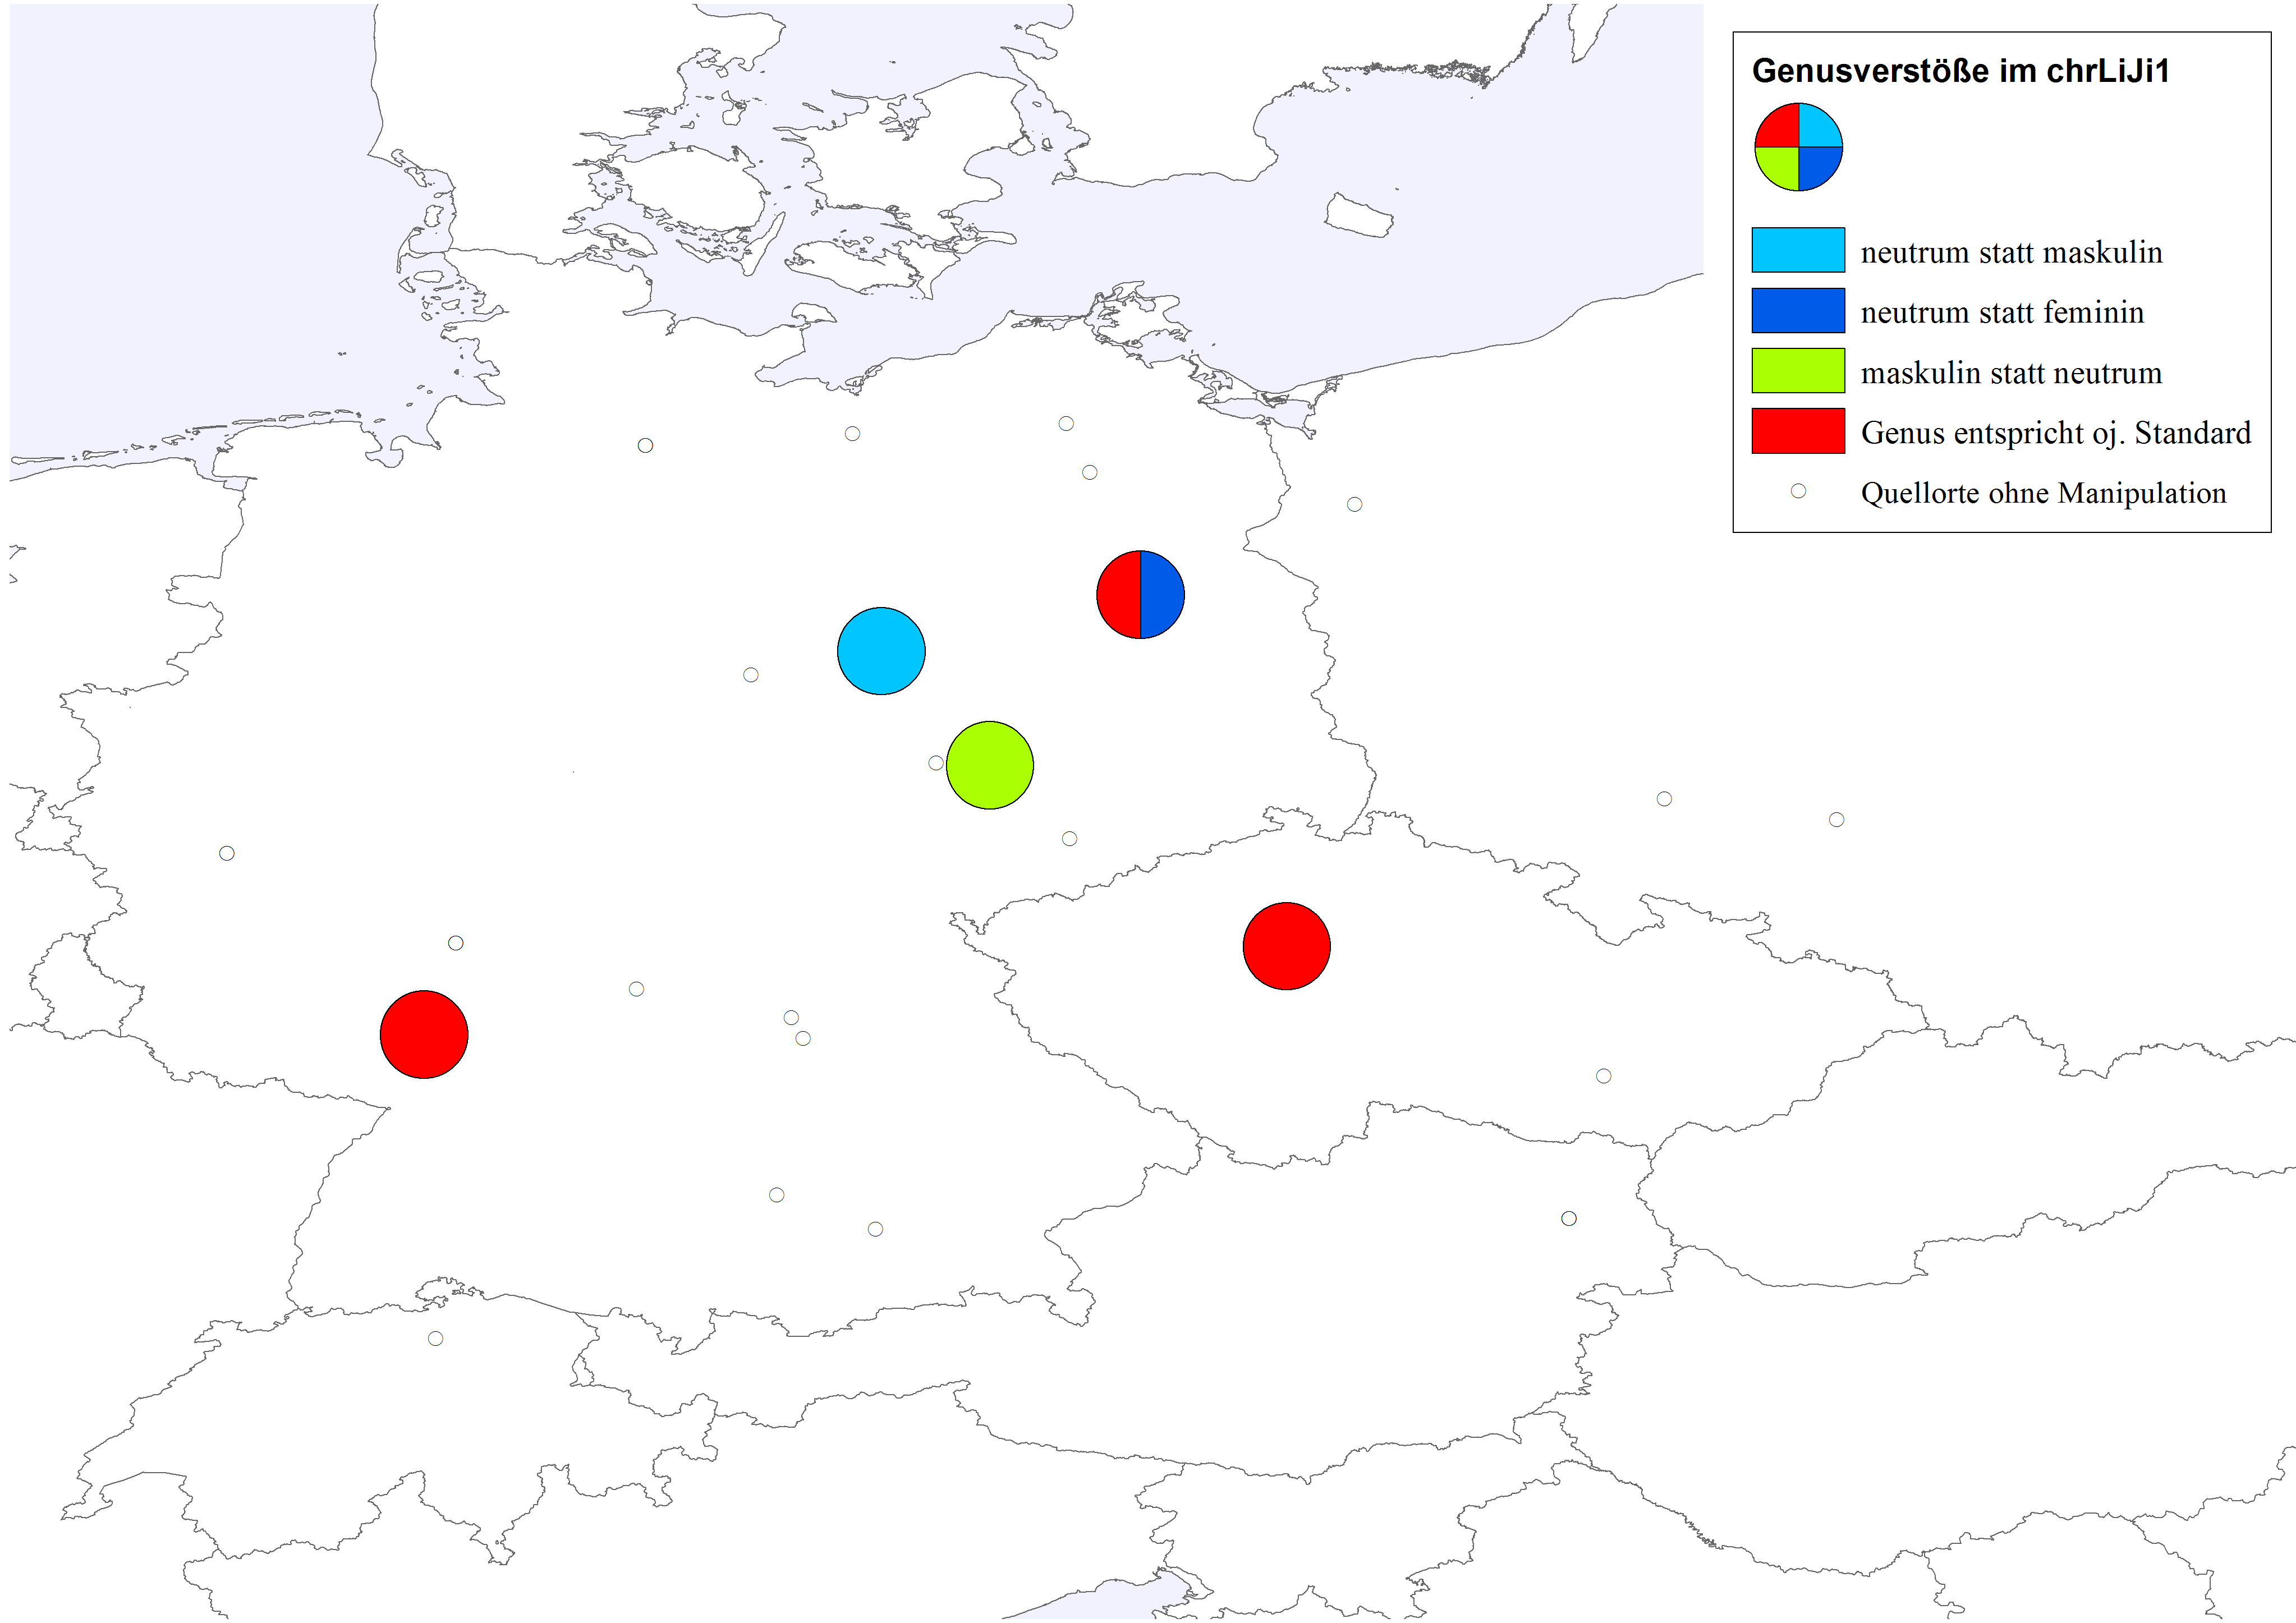
\includegraphics[width=\textwidth]{figures/KarteGenus.png}
		\caption{\label{KarteGenus} Genusverschiebungen im \hai{chrLiJi1}}
	\end{figure}
 
	 

Abschließend lässt sich festhalten, dass Genusverschiebungen von der deutschen Schriftsprache im \hai{{\LiJieins}} äußerst selten vorkommen. Die Hälfte der Belege verwenden Genera, die ostjiddischen Formen entsprechen. Dies ist erstaunlich und kann für eine Kenntnis dieser Autoren vom Ostjiddischen sprechen oder als Hinweis für ein vom Schriftdeutschen abweichendes Genussystem im Westjiddischen interpretiert werden. Wie nun die übrigen vier Belege zu interpretieren sind, muss offen bleiben. Zum einen ist es durchaus möglich, dass die entsprechenden Lexeme in den entsprechenden jiddischen Dialekten genau die Genera aufweisen, die im \hai{{\LiJieins}} belegt sind. Andererseits ist auch die pejorative Funktion von Genusverstößen nicht völlig von der Hand zu weisen. 
Plausibel erscheint es, eine Kombination zwischen Pejoration und Sprachrealität anzunehmen.


  \section{Diminutionen}\label{dim}
 %\noindent
Die \isi{Diminution} ist ein äußerst frequentes Mittel der Charakterisierung jüdischer Figuren. Es finden sich im \hai{chrLiJi1} in 39 (von 53) Quellen 12 verschiedene Diminutivsuffixe für die Singulardiminution (Tabelle \ref{tblDIMSG}, S.\, \pageref{tblDIMSG}) und in 27 Texten 14 Suffixe für die \isi{Diminution} im Plural (Tabelle \ref{tblDIMPL}, S.\, \pageref{tblDIMPL}). In vielen Texten werden dabei mehrere Suffixe parallel verwendet. Im Singular zeigen 14 Quellen zwei unterschiedliche Suffixe parallel. Insgesamt sieben Quellen verwenden drei und in jeweils einer Quelle treten vier (\hai{PA} Frankfurt, 1834) und sechs (\hai{GW} n.a., ca.\, 1900) unterschiedliche Suffixe nebeneinander auf. Der Mittelwert liegt bei 1,4 Suffixen pro Quelle (bei einer Standardabweichung von {$\sigma$}\,1,2). Sechs Quellen verwenden zwei unterschiedliche Suffixe zur Pluraldiminution; fünf Quellen drei und eine Quelle (\hai{PG} Speyer, 1835) vier Suffixe. Dies allein zeigt, welche Vielzahl an Suffixen eingesetzt wird.\label{AnzahlDIM}

Die im Jiddischen verwendeten Diminutivsuffixe entstammen der germanischen Komponente. Aus diesem Grund wird, bevor auf die \isi{Diminution} im Jiddischen eingegangen wird (Unterabschnitt \ref{dimJIDDISCH}), das deutsche System dargestellt (Unterabschnitt \ref{dimDEUTSCH}). Da das Jiddische die Unterscheidung zwischen Diminutivsingular und -plural trifft (\citealt[162–166]{Jacobs2005}), erfolgt die anschließende Analyse aufgrundlage dieser Trennung. Es werden zunächst die einzelnen im \hai{{\LiJi}}  auffindbaren Singulardiminutiva  und später die Pluraldiminutiva dargestellt und mit der Situation im Jiddischen und den deutschen Dialekten verglichen. In die Analyse nicht aufgenommen wird die semantische Kategorie des Diminutivs 1. und 2. Grades, der eine Unterscheidung zwischen \sem{verkleinernd} und \sem{verzärtlichend} trifft und für das Jiddische angenommen wird (\citealt[48]{Landau1895}; \citealt[80]{Perlmutter1988}; \citealt[162]{Jacobs2005}),\footnote{Eine solche semantische Differenzierung ist auch aus den deutschen Dialekten bekannt, wie z.\,B.\, dem Schwäbischen oder dem Hochalemannischen (vgl.\, \citealt[1250]{Seebold1983}; \citealt[159–208]{Luessy1974}; \citealt[162]{Schirmunski1962}).} da solche Kategorien bestenfalls durch direkte Sprecherbefragung, aber nur schwer aufgrundlage schriftlicher Quellen ermittelt werden können.





\subsection{Diminution in den deutschen Dialekten}\label{dimDEUTSCH}
%  %\noindent
Im Deutschen wie auch im Jiddischen erfolgt die \isi{Diminution} mittels Umlautung des Stammvokals und Suffigierung am Stamm. Für die Dialekte des Deutschen veranschlagt man abhängig vom Konsonanten des Suffixes eine grobe Einteilung in \hai{L}- und \hai{K}-\isi{Diminution} (u.\,a.\, \citealt{Wrede1908}; \citealt[475–487]{Schirmunski1962}; \citealt{Seebold1983}), d.\,h. es liegen zwei Klassen von Diminutivsuffixen vor, die sich in ihrem Basiskonsonanten unterscheiden. Dabei finden sich Diminutivformen mit -\textit{l}- als Basiskonsonant im Süden des Sprachgebiets, Formen auf -\textit{k}-(> -\textit{ch}-) im Norden (vgl.\, Abbildung \ref{tblDIMsystemSg}, S.\, \pageref{tblDIMsystemSg} u. \ref{DimDSA}, S.\, \pageref{DimDSA}).\footnote{In den dt. Dialekten der Schweiz und Österreichs, die nicht von den Wenkerkarten abgedeckt sind, setzt sich das \isi{Dialektkontinuum} fort und wir finden hier konsequent \hai{L}-\isi{Diminution}.} Diese Nord-Süd-Teilung der Dialekte spiegelt sich selbst im Schriftdeutschen wieder, wo zwei Diminutivsuffixe -\textit{chen} und -\textit{lein} gebräuchlich sind.\footnote{Mittlerweile hat sich überwiegend die ursprünglich ostmitteldeutsche Diminutivbildung mittels -\textit{chen} durchgesetzt (\citealt[475, 479]{Schirmunski1962}; \citealt[157]{Koenig1978}). Sobald der Stamm auf -\textit{ch}, -\textit{g}, oder -\textit{ng} auslautet, findet sich in der nhd. Schriftsprache die ursprünglich oberdeutsche Bildung mit -\textit{lein} (\citealt[475]{Schirmunski1962}).} Die deutschen Mundarten weisen hingegen weitaus mehr und \qu{seit langem konkurrierende Typen von Diminutivformen} auf, als die Standardsprache vermuten lässt (\citealt[476]{Schirmunski1962}). Wie \cite{Wrede1908} in seiner umfassenden Beschreibung der im Wenkermaterial erhobenen Diminutiva zeigt, ist das Auftreten eines Diminutivsuffixes in den meisten Dialekten abhängig von der \isi{Semantik} eines Lexems und dessen phonologischen Bedingungen. Tatsächlich verwenden die meisten Sprecher eines deutschen Dialekts mehr als nur ein Suffix. Die Leitformenkartierung des \hai{WA} ist damit bei diesem Phänomen stark an das einzelne Lexem gebunden (\citealt[74f]{Wrede1908}).\label{wredeDIM} Das heißt auch, dass alle nachfolgenden Kartenbilder, insbesondere die Polygone des \hai{WA}, wie auch im Fall der phonologischen Karten, nur die Variationen eines Lexems darstellen und keine Gesetzmäßigkeiten reflektieren (vgl.\, \citealt[79]{Wrede1908}). 
   
   
  Die zwei Basistypen von \isi{Diminution} bewirken je nach Vokal kleinräumige areale Variation.\, Hinzu kommen Fusionsformen beider Basistypen, wie man sie im mitteldeutschen Raum, also in der Kontaktzone zwischen \hai{L}-\, und \hai{K}-{Di\-mi\-nu\-tion}, findet. Eine Zusammenfassung der belegten Kombinationen findet sich in Tabelle \ref{tblDIMsystemSg} (S.\, \pageref{tblDIMsystemSg}) für die Singulardiminution und in Tabelle \ref{tblDIMsystem} (S.\, \pageref{tblDIMsystem}) für die Pluralformen.  
 
	Eine Trennung zwischen Singular- und Pluraldiminution, wie sie das Jiddische zeigt und welche nach den Regeln der morphologischen Natürlichkeit besondere \textit{Ikonizität} abbildet (vgl.\, \citealt[insbes. 98–102]{Mayerthaler1981}; \citealt[insbes. 59]{Wurzel1984}), kennen nur wenige deutsche Dialekte. Ausgehend von der in Tabelle \ref{tblDIMsystem} (S.\, \pageref{tblDIMsystem}) aufgeführten Typisierung werden in Abbildung \ref{DimDSA}  die Einzelformen (\hai{WA}-Karte Nr. 381) zur Pluraldiminution zu entsprechenden Polygonen zusammengefasst, die die einzelnen Typen und ihre räumliche Verbreitung darstellen.\footnote{Das Suffix \textit{-chen} verhält sich in der Typisierung als Pluraldiminutivsuffix problematisch, da es zum einen dem Typ einfacher \hai{K}-\isi{Diminution} zugerechnet werden kann; gesetzt den Fall es bestünde aus dem Diminutivsuffix \textit{-chen-} zuzüglich einem  \textit{-en}-Plural ist es zum anderen aber auch dem Typ \hai{K}+\hai{{\Pl}} zuzurechnen. Der Vergleich der Karten zum Singular- und \isi{Pluralsuffix} im \hai{WA} (Karten 381 u. 440) zeigt, dass im ostmitteldeutschen (insbes. dem Obersächsischen) \textit{-chen} sowohl als übliches Suffix zur Singular- als auch zur Pluraldiminution vorliegt. Damit ist keine Unterscheidung zwischen Singular und Plural bei der \isi{Diminution} erkennbar und das Suffix muss hier  zum einfachen \hai{K}-Typ gerechnet werden. Anders sieht es jedoch im Rheinfränkischen (insbes. zwischen Aschaffenburg u.  Weinheim) aus. Hier finden sich im Singular die Suffixe \textit{-che}, \textit{-elche}, \textit{-el} und \textit{-la}. Wir haben es also mit einer äußerst vielfältigen Region von Diminutivsuffixen im Singular zu tun. Im Plural aber findet sich hier flächendeckend \textit{-chen}. Damit unterscheidet sich das Suffix eindeutig vom Singular und die Analyse des Suffix als \hai{K}-\isi{Diminution} + \hai{{\Pl}}-Suffix erscheint hier sinnvoll, zumindest gilt dies für die Gebiete, in denen \textit{-che} und \textit{-elche} im Singular vorliegen. Aus diesem Grund wurde das entsprechende Gebiet im Rheinfränkischen in Karte \ref{DimDSA} zum \hai{K}+\hai{{\Pl}}-Gebiet gezählt, während das Gebiet im Obersächsischen, welches \textit{-chen} im Singular und im Plural aufweist, als zur reinen \hai{K}-\isi{Diminution} gehörig kartiert wurde.} Augenscheinlich ist die aus der Singulardiminution bekannte Nord-Süd-Teilung in \hai{K}- und \hai{L}-\isi{Diminution} (vgl.\, Abbildung \ref{SgDimDSA}). Ebenfalls fällt auf, dass eine besondere Pluralmarkierung vor allem in Regionen von \hai{K}-Singulardiminution und besonders im (west-)mitteldeutschen Gebiet verwendet wird. Im Süden hingegen, wo die \hai{L}-\isi{Diminution} verbreitet ist, wird kaum zwischen Plural und Singular am Diminutivum unterschieden. Die Kombination von \hai{L}-\isi{Diminution} im Singular und \hai{K + {\Pl}}-\isi{Diminution} im Plural, wie sie im Jiddischen vorliegt, ist eine seltene Ausnahme im deutschen Dialektverbund. Lediglich in den Randgebieten des Rhein- und Ostfränkischen kann man  die auf \hai{L}-\isi{Diminution} aufbauenden Pluraldiminutivsuffixe finden und hierbei unter anderem auch das aus dem Jiddischen bekannte Suffix \textit{-lich}. Dieses Suffix findet sich entlang der Isoglosse von \hai{L}- und \hai{K}-Diminutionstypen. Es ist v.\,a.\, diese geolinguistische Verortung, die dafür spricht, in dem Suffix eine Fusion der beiden Basistypen von \isi{Diminution} zu sehen, wie sie auch bei anderen Suffixen entlang der \hai{L}/\hai{K}-Isoglosse zu finden ist.\footnote{So wird der Fusionscharakter von Diminutivsuffixen im Mitteldeutschen deutlicher am Beispiel des Suffixes \textit{-elcher}, welches als eine Fusion aus \textit{-el}\textsubscript{\hai{L}-{\Dim}} + \textit{-ch(e)}\textsubscript{\hai{K}-{\Dim}} + \textit{-(e)r}\textsubscript{{\Pl}} zu analysieren ist.} \\
	
	
	
	 
  
  \begin{table}
%\begin{longtable}{cccccc}

		\begin{tabular}{ll}

		\lsptoprule 

\textbf{Muster} &\textbf{Beispiel} (\sem{Ente\textsubscript{{\Dim} {\Sg}}})  \\ \midrule 

\hai{K} & \textit{-che} \textit{Entche}, \textit{-ke} \textit{Entke} \\
\hai{L} & \textit{-le} \textit{Entla}, \textit{-ile} \textit{Entile} \\

\hai{L + K }& \textit{-elche} \textit{Entelche} \\
  \lspbottomrule 
 \end{tabular}
		 \caption{Grundmuster von Singulardiminutivsuffixen im Deutschen (basierend auf \hai{WA} Karte Nr. 440 \sem{Stückchen})}
		 \label{tblDIMsystemSg}
		 \end{table}
		% \end{longtable}
 

	
	  \begin{figure} 

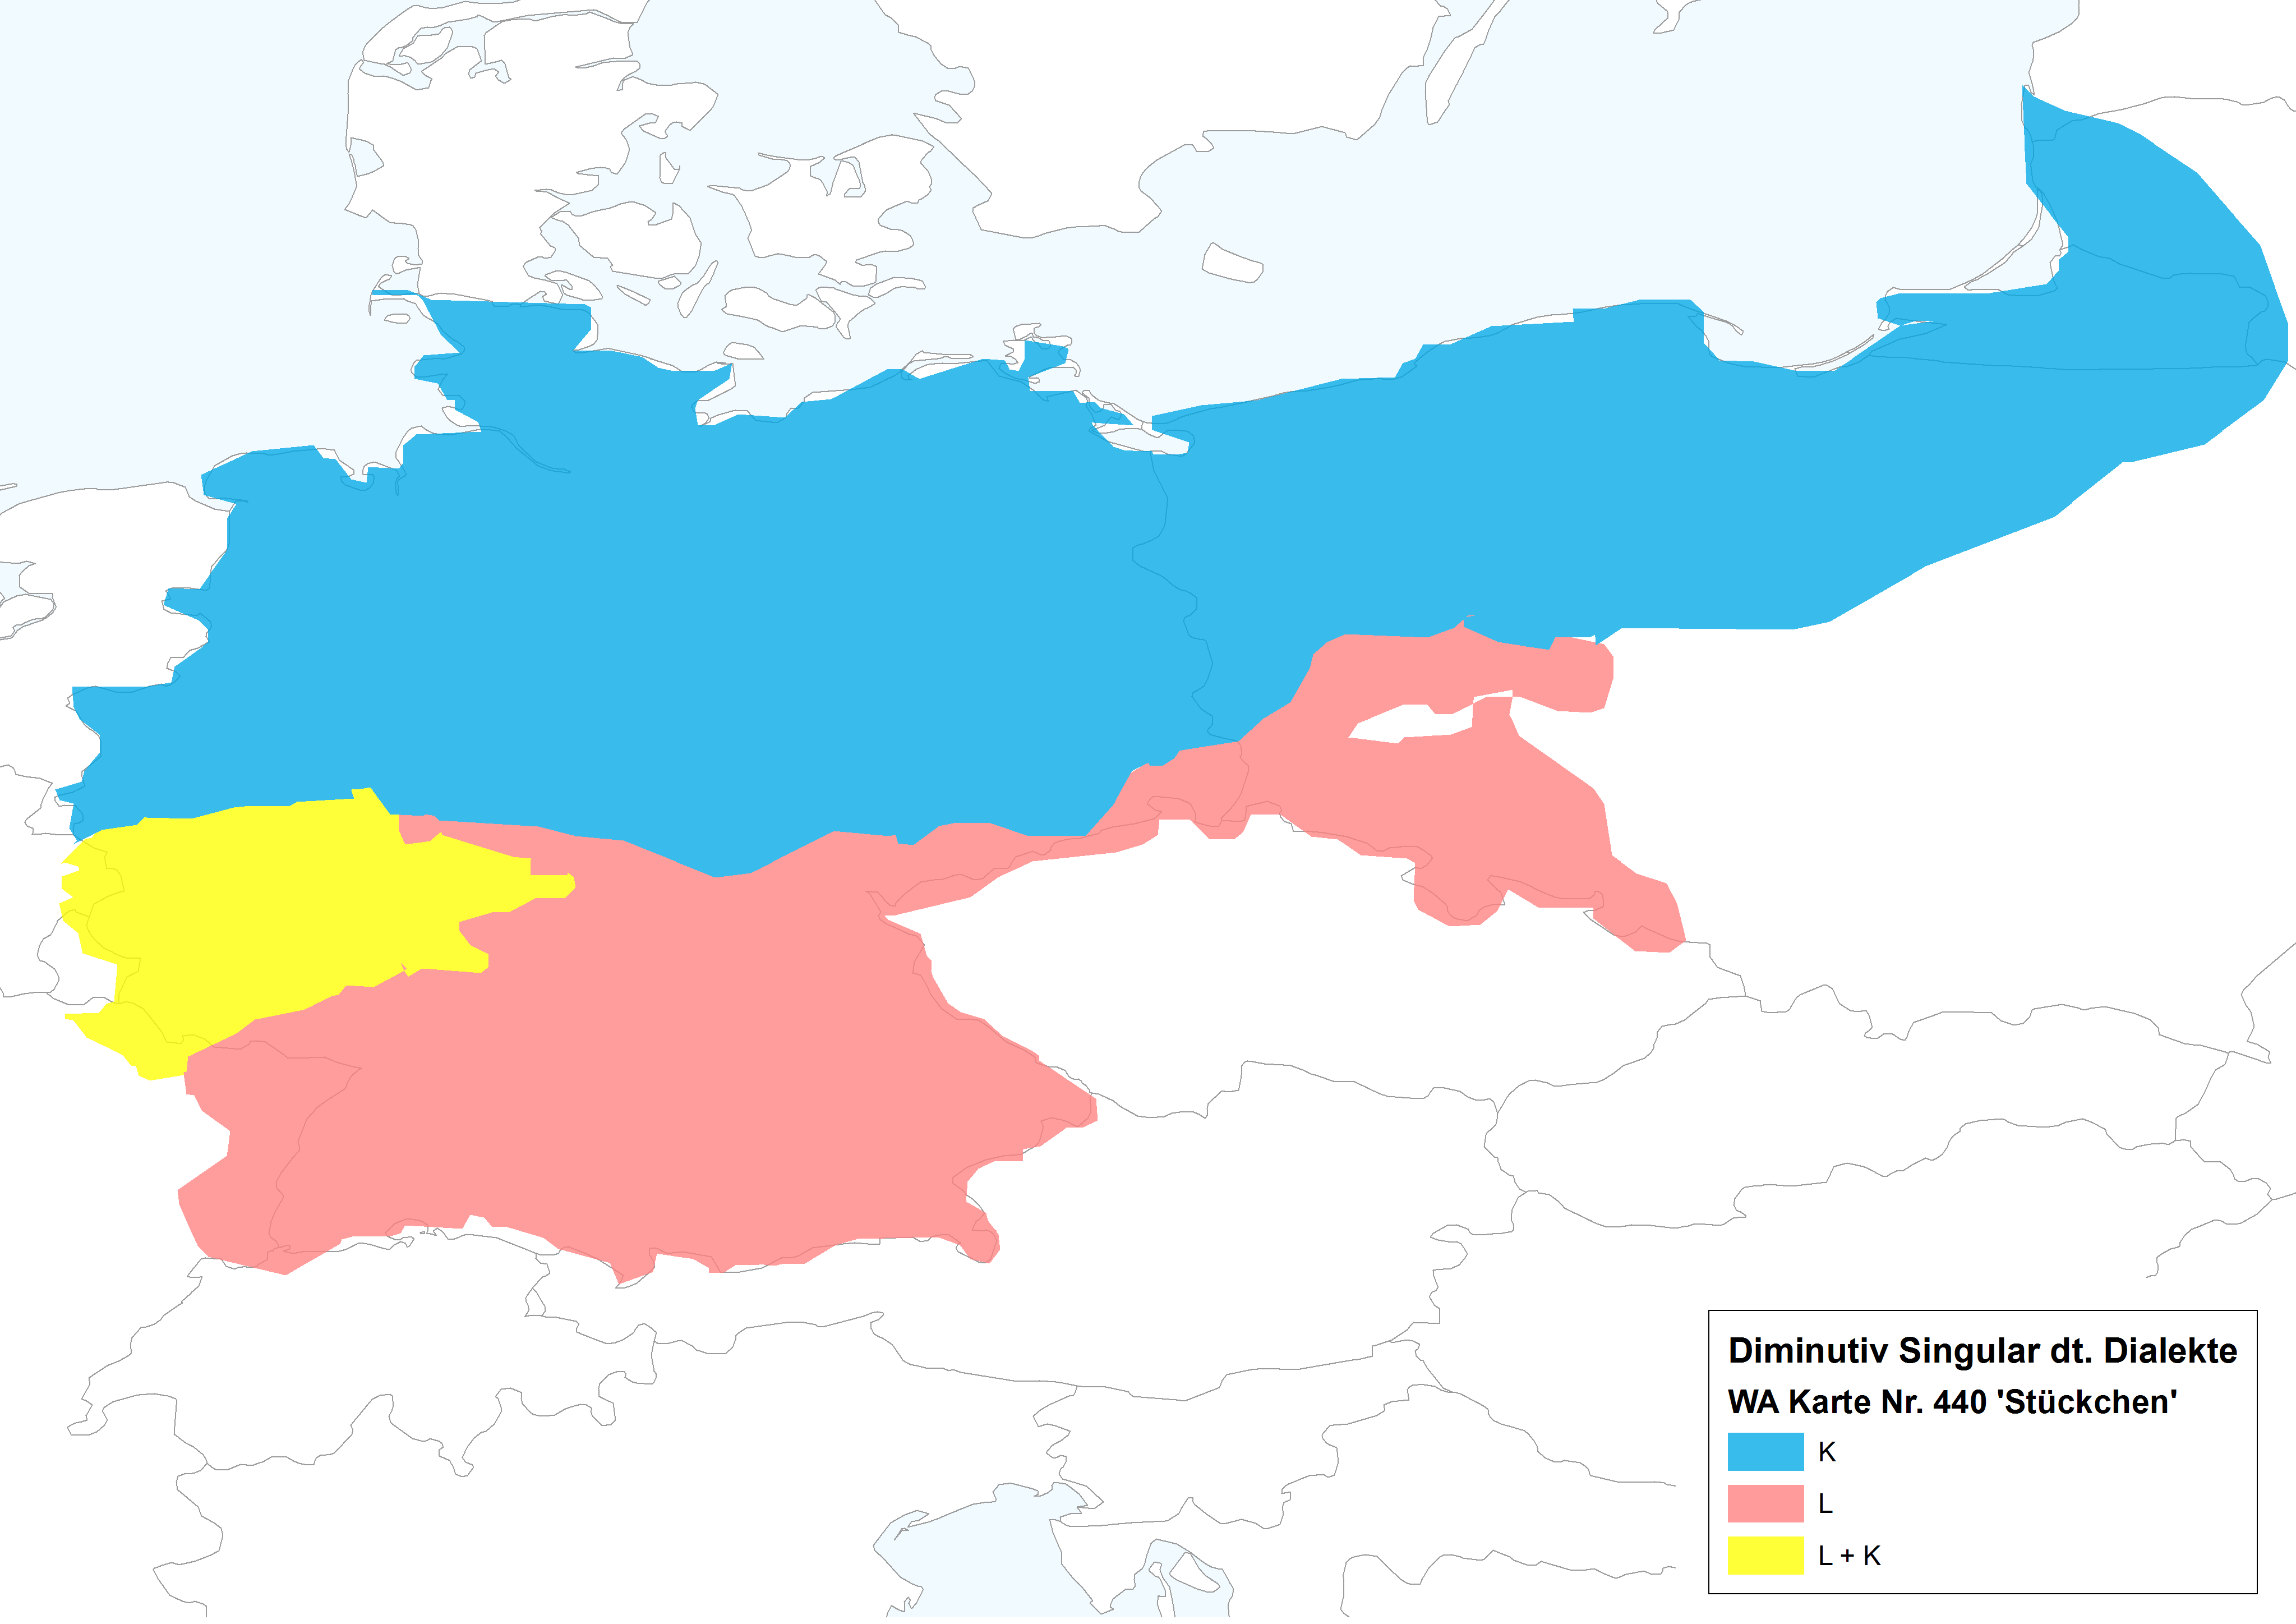
\includegraphics[width=\textwidth]{figures/DSA_DIM_SG_kurz.png}
		\caption{\label{SgDimDSA} Singulardiminutionen in den dt. Dialekten (\hai{WA} Karte Nr. 440 \sem{Stückchen})}
		\end{figure}
 


	
		
		
		
  \begin{table}
%\begin{longtable}{cccccc}

		\begin{tabular}{ll}

		\lsptoprule 

\textbf{Muster} &\textbf{Beispiel} (\sem{Ente\textsubscript{{\Dim} {\Pl}}})  \\ \midrule 

\hai{K} & \textit{-che} \textit{Entche}, \textit{-ke} \textit{Entke} \\
\hai{L} & \textit{-le} \textit{Entla}, \textit{-ile} \textit{Entile} \\

\hai{L + K }& \textit{-lich} \textit{Entlich} \\
\hai{K + L }& \textit{-chel} \textit{Entchel} \\ 

\hai{{\Pl} + K }& \textit{-erche} \textit{Enterche}, \textit{-erje} \textit{Enterje} \\
\hai{{\Pl} + L }& \textit{-erle} \textit{Enterle}\\

\hai{K + {\Pl}} & \textit{-kes} \textit{Entkes}, \textit{-cher} \textit{Entcher} \\
\hai{L + {\Pl}} & \textit{-len} \textit{Entlen} \\


\hai{{\Pl} + K + {\Pl}} & \textit{-ercher} \textit{Entercher}, \textit{-erchens} \textit{Enterchens} \\

  \lspbottomrule 
 \end{tabular}
		 \caption{Grundmuster von Pluraldiminutivsuffixen im Deutschen (basierend auf \hai{WA} Karte Nr. 381 \sem{Apfelbäumchen})}
		 \label{tblDIMsystem}
		 \end{table}
		% \end{longtable}
		
 

 \begin{figure} 

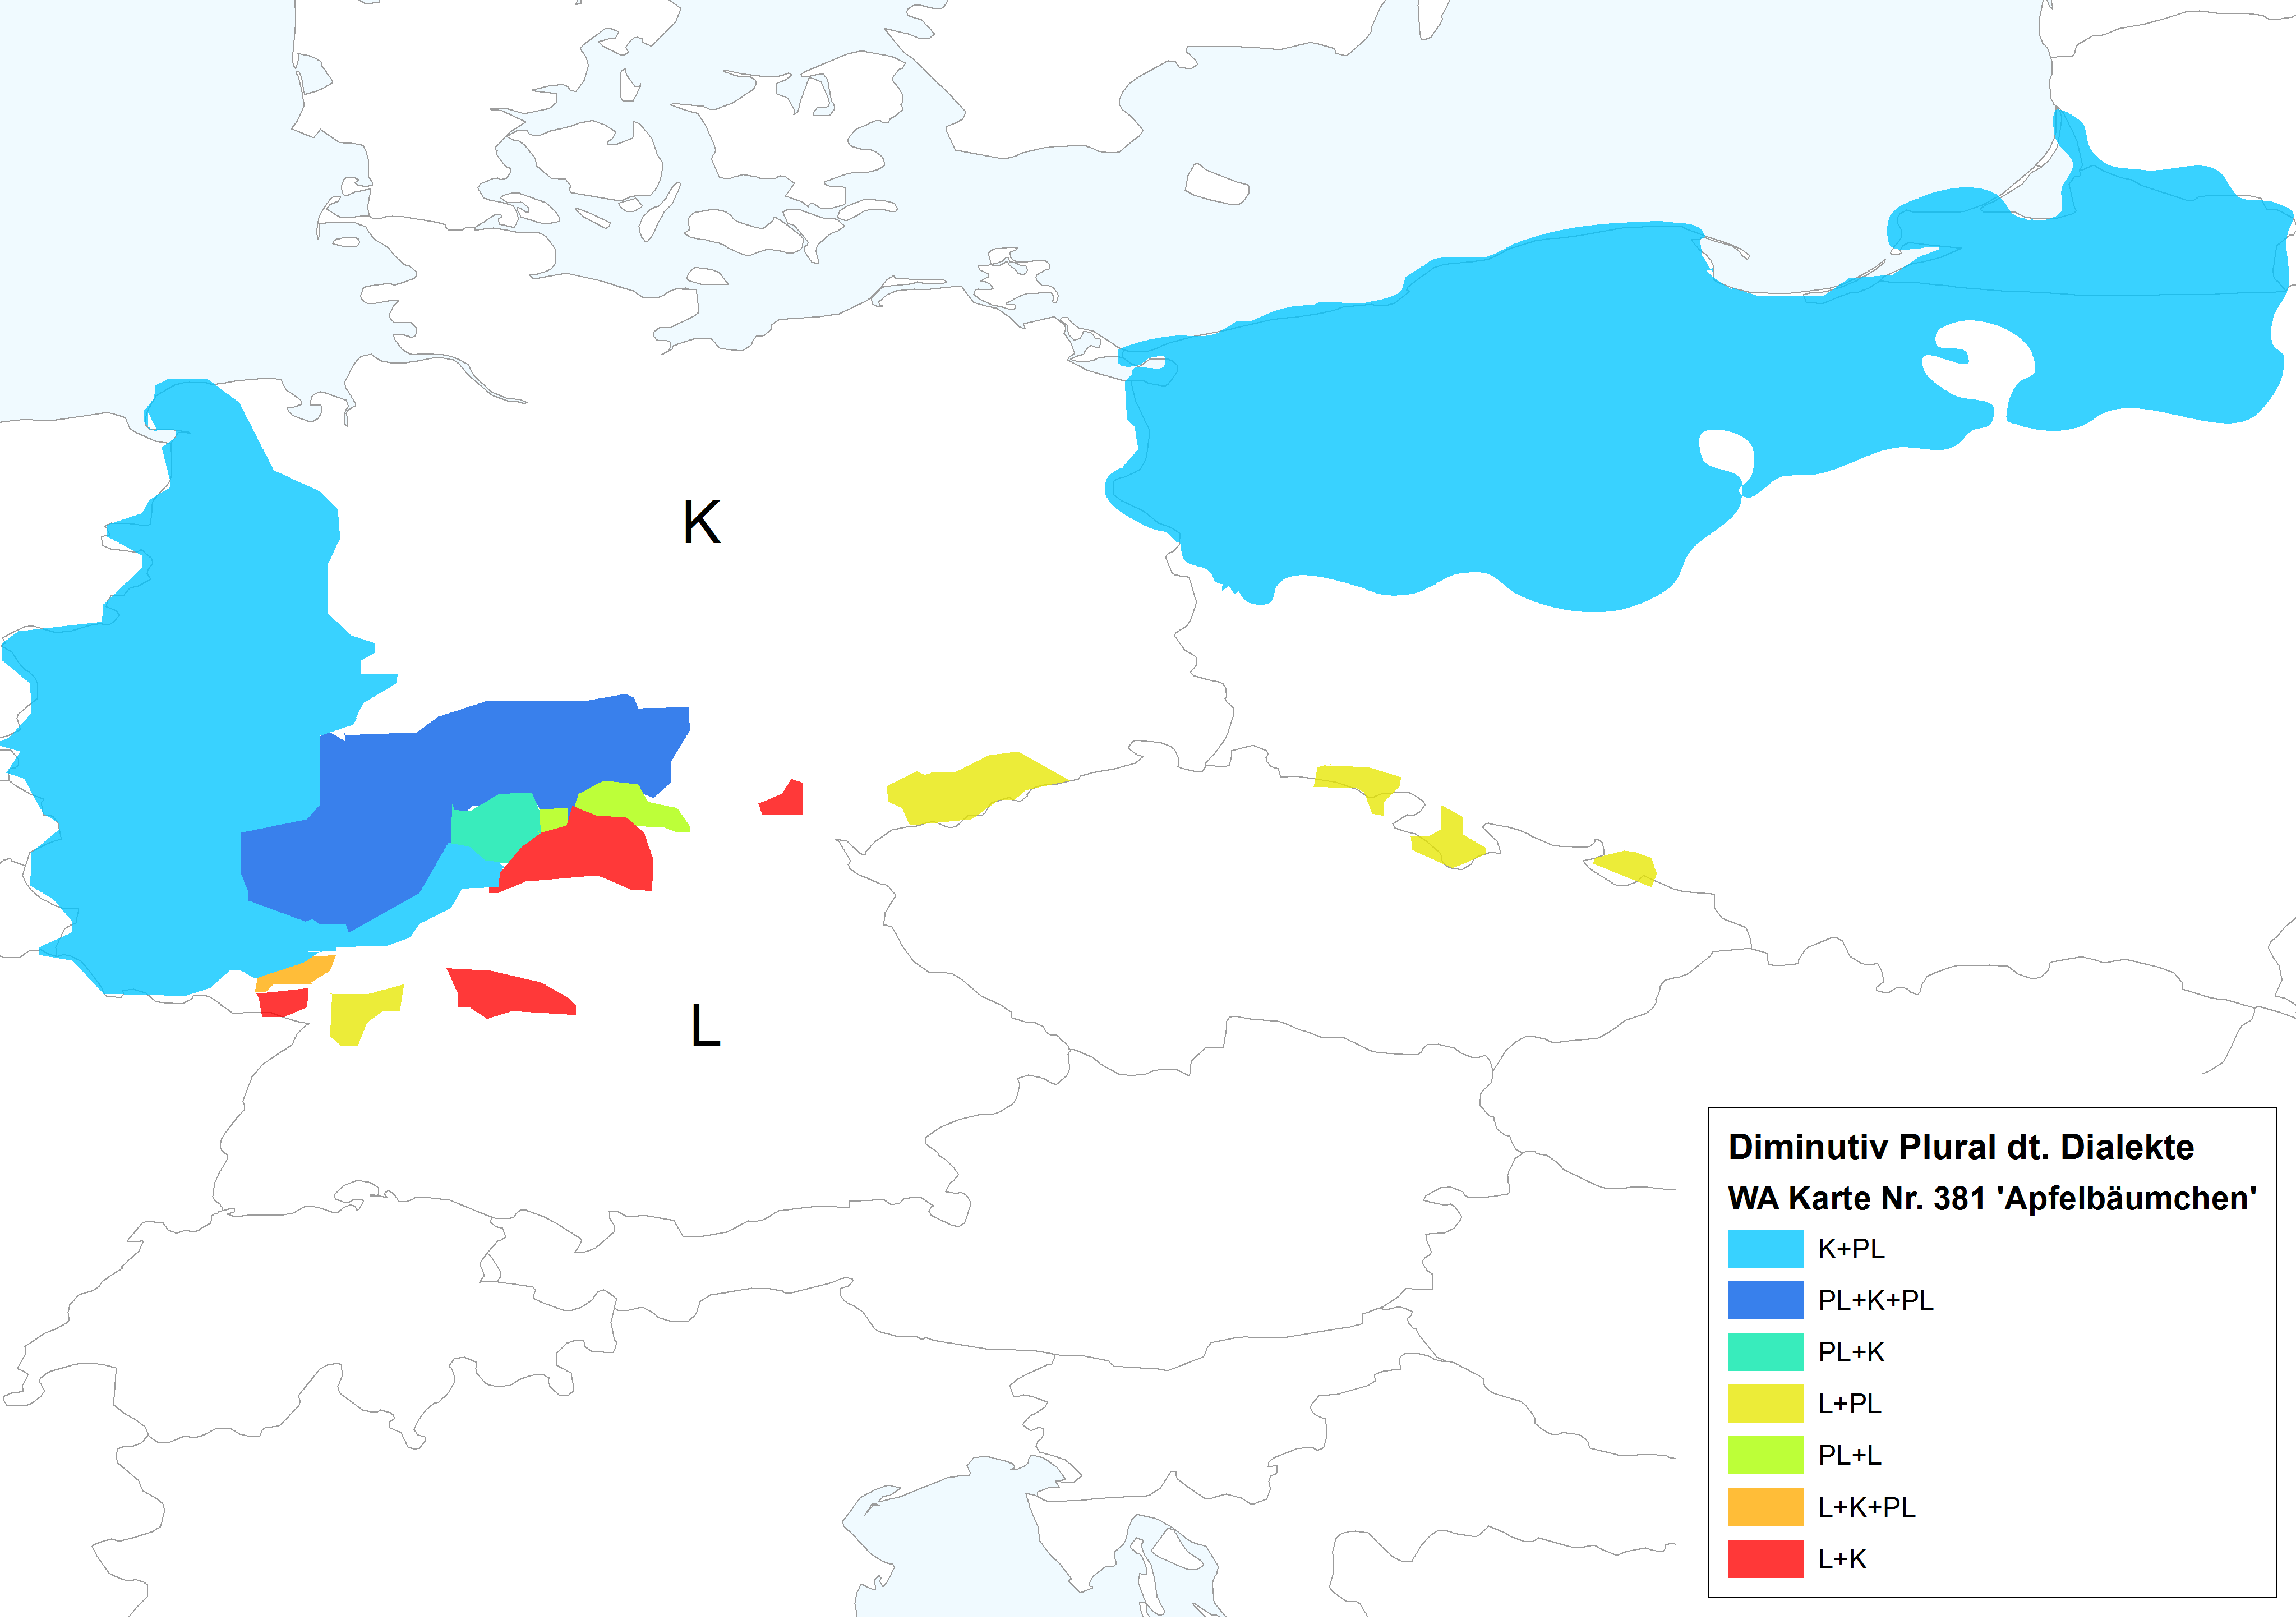
\includegraphics[width=\textwidth]{figures/DSA_DIM_PL_kurz.png}
		\caption{\label{DimDSA} Pluraldiminutionen in den dt. Dialekten (\hai{WA} Karte Nr. 381 \sem{Apfelbäumchen})}
		\end{figure}



\subsection{Diminution im Jiddischen}\label{dimJIDDISCH}
%  %\noindent

\largerpage[-2] 
Das Diminutionssystem des modernen Ostjiddischen fasst Tabelle  \ref{tblDIMOJ} zusammen. Der Singular wird mittels -\textit{l} (1. Grad) und -\textit{ele} (2. Grad)\footnote{Das Suffix -\textit{ele} findet sich auch bei auf /l/ auslautenden Nomina auch im 1. Grad, z.\,B.\, \RL{{{פ\makebox(-0.8,7)[r]{\libertineGlyph{uni207B}}}}ויגל} 
\textit{foygl} \sem{Vogel} \RL{{{פ\makebox(-0.8,7)[r]{\libertineGlyph{uni207B}}}}ייגעלע} 
\textit{feygele} \sem{Vogel\textsubscript{{\Dim} {\Sg}}}} gebildet (\citealt[69]{Jacobs2005}; \citealt[80]{Perlmutter1988}). Die Pluraldiminution wird mittels -\textit{lekh} (1. Grad) bzw. -\textit{elekh} (2. Grad) gebildet (\citealt[162–163]{Jacobs2005}; \citealt[80]{Perlmutter1988}). Bei Nomina mit \ili{hebräisch}-aramäischer \il{hebräisch} Wurzel findet sich oftmals eine doppelte  Pluralmarkierung, indem \textit{-(e)lekh} an das bereits im Plural stehende Nomen gehängt wird, wie z.\,B.\, in \RL{חסיד} \textit{khsid} \sem{Frommer\textsubscript{{\Sg}}} > \RL{חסידים} \textit{khsidim} \sem{Fromme\textsubscript{{\Pl}}} > \RL{חסידיםלעך} \textit{khsidimlekh} \sem{Frommer\textsubscript{{\Pl}+ {\Dim} {\Pl}}} (\citealt[163]{Jacobs2005}; \citealt{Perlmutter1988}). Dieselbe Situation lässt sich aber auch in einzelnen Lexemen der germanischen Komponente finden, z.\,B.\, in \RL{קינדערלעך} \textit{kinderlekh} \sem{Kind\textsubscript{{\Pl} + {\Dim} {\Pl}}} (\citealt[163]{Jacobs2005}; \citealt{Perlmutter1988}). Jiddisch orientiert sich damit an der \hai{L}-\isi{Diminution}, die im Ober- und Mitteldeutschen verbreitet ist. Das \isi{Pluralsuffix} findet sich in den deutschen Dialekten des Ost- und Rheinfränkischen als -\textit{lich} belegt, wo es sich entlang der Isoglosse zwischen \hai{L}- und \hai{K}-\isi{Diminution} als Fusionsform beider Formen herausgebildet hat (\citealt[647]{Grimm1890}; \citealt[245]{Weinhold1867}; \citealt[124]{Wrede1908}; \citealt[49]{Paul1920}).\footnote{Die Analyse des Suffixes als Fusion der zwei Basistypen von \isi{Diminution} wird nicht von jedem geteilt. Z.\,T. wird dieses Suffix als \isi{Komposition} von \hai{L}-\isi{Diminution} und dem Kollektivsuffix {\ahd} -\textit{ahi}, {\mhd} -\textit{ech} (-\textit{ach}, -\textit{ich}), nhd. -\textit{icht} (un\isi{produktiv} z.\,B.\, in \textit{Kehricht}, \textit{Dickicht}) analysiert, so etwa in \cite[484]{Schirmunski1962} oder \cite[110–112]{Timm2005}. \cite[235]{Weinhold1867} schlägt vor, dass die Existenz des Kollektivsuffixes als Katalysator für die Grammatikalisierung der Fusionsform als \isi{Pluralsuffix} gewirkt haben mag. Ebenso können auch die -\textit{ach}-Plurale des Oberdeutschen dazu beigetragen, der Fusionsform -\textit{lich} Pluralbedeutung zu geben (vgl.\, \citealt{Rowley1994}).}\\ 



 \begin{table}
%\begin{longtable}{ccc|ccc}

		\begin{tabular}{llllll}

	\lsptoprule

\textbf{Grad} &\textbf{Numerus} & \textbf{Suffix} & \multicolumn{2}{c}{\textbf{Beispiel \sem{Lied}}} \\ 
\midrule 

1. & {\Sg} & -\textit{l} & \RL{לידל} & \textit{lidl} &\sem{kleines Lied} \\

1. & {\Pl} & -\textit{lekh} & \RL{לידלעך}& \textit{lidlekh} &\sem{kleine Lieder} \\ %format?!   andere Zeilentrennung überlegen? \hdashline?

2. & {\Sg} & -\textit{ele} &  \RL{לידעלע} &\textit{lidele}& zärtlich \sem{Lied} \\ 

2. & {\Pl} & -\textit{elekh} &\RL{לידעלעך} &\textit{lidelekh}& zärtlich \sem{Lieder} \\
 
 
 
\lspbottomrule
 \end{tabular}
		 \caption{Das Diminutionssystem des standardisierten Ostjiddischen}
		 \label{tblDIMOJ}
		 \end{table}
		% \end{longtable}


Die Situation der \isi{Diminution} in den jiddischen Dialekten ist bislang noch nicht beschrieben worden. Die Daten des \hai{LCAAJ} (\citeyear[120]{Herzog2000}) lassen vermuten, dass es tatsächlich diatopisch unterschiedliche Suffixe gab und womöglich auch das System der graduellen Diminuierung de facto nicht soweit verbreitet war, wie das standardisierte Jiddisch vermuten lässt.\footnote{Die Daten zur \isi{Diminution} des \hai{LCAAJ} (\citeyear[120–125, insbes. Karte 36]{Herzog2000}) bieten nur einen minimalen Ausschnitt in die tatsächliche Sprachsituation. Dies zeigt sich besonders daran, dass hier im Singular zwei unterschiedliche und nicht miteinander vergleichbare Suffixe (\RL{שיקסע} \textit{shikse} \sem{Nichtjüdin} im Westjiddischen und \RL{מויל} \textit{moyl} \sem{Mund} im Ostjiddischen) die Basis bilden. Wie \cite{Wrede1908} zeigt, ist die Wahl eines Diminutivsuffixes stark lexemgebunden, vgl.\, S.\, \pageref{wredeDIM}. Hinzu kommt, dass die Erhebungsmethode des Fragebogens im Westjiddischen kaum dazu ausreichte,  semantische Feinheiten wie die \isi{Diminution} 1. und 2. Grades einzufangen.} Dialektale Abweichungen vom Standard finden sich zum Beispiel im \hai{{\NOJ}}, wo die Singulardiminuierung von  \RL{מויל} \textit{moyl} \sem{Mund}  mittels -\textit{kh(e)le} erfolgt, und im \hai{{\SOJ}} findet sich das Suffix -\textit{lche(n)} im Lexem \RL{שיקסע} \textit{shikse} \sem{Nichtjüdin} (\citealt[122, Karten Nr. 36S1, 36S2]{Herzog2000}). \,%rs + "Nr."
Wie in den deutschen Dialekten herrscht so scheinbar auch in den jiddischen Varietäten eine vom Lexem abhängige Vielfalt an Diminutivsuffixen vor (vgl.\, S.\, \pageref{wredeDIM}). Vor allem aber fällt die Datenmenge des \hai{LCAAJ} zu gering aus, als dass sich auf deren Basis Aussagen über das jiddische Diminutionssystem machen ließen.\label{SOJDIM}

Dies zeigt sich besonders im Westjiddischen. Den Daten des \hai{LCAAJ} (\citeyear[120–125]{Herzog2000}) zufolge bildet das Westjiddische die Singulardiminution im \hai{{\SWJ}} und südwestlichen \hai{{\ZWJ}} mittels -\textit{(e)le}, im \hai{{\NWJ}} und \hai{{\NÜJ}} mittels -\textit{l}, im \hai{{\SÜJ}} finden sich beide Suffixe parallel und im westlichen \hai{{\ZWJ}} ist -\textit{che(n)} zu finden (\citealt[120–122, Karten Nr. 36, Nr. 36S1]{Herzog2000}). \citeauthor{GuggenheimGruenberg1973}s Daten zum südlichen \hai{{\SWJ}} und \hai{{\ZWJ}} bestätigen dieses Bild nicht; vielmehr finden sich hier die den koterritorialen deutschen Dialekten entsprechenden Suffixe (\citealt[92, Karte Nr. 33]{GuggenheimGruenberg1973}). Dieses Bild bestätigen auch schriftliche Quellen aus dem 19. und 20. Jahrhundert. So findet sich im Westjiddischen nördlich des Mains die \hai{K}-\isi{Diminution} (\ref{BspSGWJ1}–\ref{BspSGWJ3}) und im Süden \hai{L}-\isi{Diminution} (\ref{BspSGWJ4}–\ref{BspSGWJ6}). \label{DIMSGWJ}

 \eenumsentence{
 
 \item \textit{Stickche} \sem{Stück\textsubscript{{\Dim} {\Sg}}}  \\
 \textit{Schnüpfche} \sem{Schnupfen\textsubscript{{\Dim} {\Sg}}} \\
(\qu{Das verfrühte Schulenrufen} Aurich 1902 [\citealt[67]{Reershemius2007}])  \label{BspSGWJ1}
 
  \item \textit{Goichen} \sem{Nichtjude\textsubscript{{\Dim} {\Sg}}} \\
  (\qu{Die Lebenserinnerungen des A. H. Heymann}, Strausberg (Berlin), 1909:\,92 [\citealt[39]{Schaefer2010}])  \label{BspSGWJ2}


 \item \RL{תמרכה} \textit{tamarche} \sem{Tamara\textsubscript{{\Dim} {\Sg}}} \\
 \RL{גומפלכה}  \textit{gumplche} \sem{Gumpel\textsubscript{{\Dim} {\Sg}}} \\
 (\qu{Die Hochzeit zu Grobsdorf} 1822:\,dramatis personae) \label{BspSGWJ3}
 
  
   \item \textit{Großvaterle} \sem{Großvater\textsubscript{{\Dim} {\Sg}}}  \\
   (\qu{Die Juden von Zirndorf} Fürth, 1897 [1996]:\,177)\label{BspSGWJ4}
   
    \item \textit{Stickle} \sem{Stück\textsubscript{{\Dim} {\Sg}}}  \\
    \textit{Peckle} \sem{Packet\textsubscript{{\Dim} {\Sg}}}  \\
      (\qu{Garkisch} Mulhouse, 1930:\, 9; 20) \label{BspSGWJ5}
      
            
    \item \textit{Stickl} \sem{Stück\textsubscript{{\Dim} {\Sg}}}  \\
     \textit{Majerl} \sem{Mauer\textsubscript{{\Dim} {\Sg}}}  \\
 (Wenkerbogen aus Frauenkirchen Nr. 42663/300447; vgl.\, \citealt{FleischerSchaeferErsch}) \label{BspSGWJ6}
 
 }

Der \hai{LCAAJ} erweckt mit der einzigen Kartierung eines durchaus problematischen\footnote{Problematisch an diesem Lexem als Stellvertreter der Pluraldiminution ist, dass die \isi{Diminution} bereits erstarrt sprich lexikalisiert, sein könnte. vgl.\, dazu auch den westjiddischen Beleg in (\ref{bspDIMPLlichAURICH}) S.\, \pageref{bspDIMPLlichAURICH} (\citealt[133]{Reershemius2007}).} 
Lexems mit Pluraldiminution \RL{קרעפלעך} \textit{kreplekh} \sem{Knödel\textsubscript{{\Dim} {\Pl}}} den falschen Eindruck, dass das Westjiddische über keine vom Singular distinkte Pluraldiminution wie das Ostjiddische verfügt. Der westlichste Beleg für die \isi{Diminution} mittels -\textit{lekh} im \hai{LCAAJ} findet sich in Prag. Dies ist ein besonders eindrucksvolles Beispiel für die Unzulänglichkeit der westjiddischen Daten des \hai{LCAAJ}, denn selbst \cite[94, Karte Nr. 34]{GuggenheimGruenberg1973} gelingt es, die westjiddische Pluraldiminution mittels -\textit{lich} einzufangen. \cite[56]{Zuckerman1969}, dessen Daten eigentlich in die Kartierung des \hai{LCAAJ} hätten einfließen müssen, findet dieses Suffix im Elsässer Jiddisch. Die ersten Belege für Pluraldiminutivbildungen auf -\textit{lich} sind aus dem Mitteljiddischen, d.\,h. aus dem 15. bis 17. Jahrhundert, bekannt (\citealt[112]{Timm2005}). Das historische Diminutivsystem des Jiddischen zeigt noch generell eine hohe Vielfalt der Suffixe (\citealt[109–113]{Timm2005}). Damit ist anzunehmen, dass das moderne System, wie es Tabelle \ref{tblDIMOJ} zeigt, tatsächlich eine Idealisierung eines wahrscheinlich wesentlich komplexeren Systems darstellt. Tatsächlich lässt sich im Fall der Pluraldiminution ein Ost-West-Gefälle innerhalb des jiddischen Dialektgebiets erkennen: Aus dem Westjiddischen sind uns bislang lediglich Quellen mit dem Suffix -\textit{lich}/-\textit{lisch} (\ref{bspDIMPLlich}–\ref{bspDIMPLlisch}) überliefert, im \hai{{\NÜJ}} findet sich vereinzelt das Suffix -\textit{lech} (\ref{bspDIMPLlechHeymann}–\ref{bspDIMPLlech}) und im \hai{{\SÜJ}} und südwestjiddischen Randgebieten zum \hai{{\SÜJ}} -\textit{loch} und -\textit{lach} (\ref{bspDIMPLloch}–\ref{bspDIMPLlach}). Allem Anschein nach ist also die Wahl des Vokals eine regional variierende Komponente. Hinzu kommt, dass im Westjiddischen nördlich des Mains das sonst für das Jiddische übliche \isi{Pluralsuffix} -\textit{l}- +  Vokal + -\textit{ch} nur in zwei umstrittenen Belegen vorliegt.\footnote{Diese beiden Belege sind in den  (\ref{bspDIMPLlichAURICH}) u. (\ref{bspDIMPLlechHeymann}) angeführt. Der Beleg aus Aurich kann, wie \citet[133 Fn. 199]{Reershemius2007} anführt, als ostjiddisches \isi{Lehnwort} im Diminutiv Plural erstarrt sein. Ebenfalls ein ostjiddischer Einfluss ist im Beleg aus Strausberg möglich, da auch dieses Lexem nicht im Westjiddischen belegt ist, vgl.\, \cite[40f]{Schaefer2010}. Die Wahl des Vokals im Diminutivsuffix spricht jedoch in beiden Fällen dafür, dass hier eine regionale Form vorliegt und nicht eine aus dem Ostjiddischen entlehnte.} Das allgemeine Bild westjiddischer (Plural-)\isi{Diminution} im Norden des Sprachgebiets scheint eine größere Variation zu haben, als es im Südwesten der Fall ist. Ein eindrucksvolles und glaubwürdiges Beispiel ist hier \qu{Die Hochzeit zu Grobsdorf}, in der eine hohe Varianz an Diminutivsuffixen im Plural\footnote{Im Singular findet sich hier regulär \RL{כה}- \textit{-che}. Die Pluralsuffixe, wie auch das Singularsuffix, können selbstverständlich aus dem Kontakt zu den koterritorialen hessischen Dialekten ins örtliche Jiddisch Eingang gefunden haben, da dort eben solche Suffixe gebräuchlich sind, vgl.\, \hai{WA} Karten Nr. 381, 440; \cite[86]{Friebertshaeuser1987}.} vorliegt (\ref{bspDIMPLgrob}). Wichtig ist festzuhalten, dass kein im Jiddischen vorkommendes Suffix auch in einem deutschen Dialekt belegt ist.\footnote{Es besteht selbstverständlich die generelle Möglichkeit, dass im Ostjiddischen \isi{Diminution} auch mittels slawischer Suffixe (insbes. -\textit{ke}) gebildet werden können. Eine umfassende Untersuchung zum ostjiddischen Diminuierungssystem müsste diesen Fall zumindest berücksichtigen, da das Suffix selbst (wenn auch un\isi{produktiv}) in vielen Lexemen der slawischen  Komponente vorhanden ist, z.\,B.\, \RL{קא\makebox(-1.5,-6.5)[r]{\libertineGlyph{uni207B}}טשקע} \textit{katshke} \sem{Ente} (vgl.\, {\poln} \textit{kaczka} \sem{Ente}), \RL{מא\makebox(-1.5,-6.5)[r]{\libertineGlyph{uni207B}}רגעריטקע} \textit{margeritke} \sem{Gänseblümchen} (vgl.\, {\poln} \textit{margerytka} \sem{Gänseblümchen}).} 


 \eenumsentence{

\item \RL{מא\makebox(-1.5,-7.5)[r]{\libertineGlyph{uni207B}}דליך} \textit{madlich} \sem{Mädchen\textsubscript{{\Dim} {\Pl}}} \\
\RL{הורג-ליך} \textit{horeg-lich} \sem{Zwerg\textsubscript{{\Dim} {\Pl}}}\\
(\qu{Esther. Oder die belohnte Tugend} Fürth, 1854:\, 7; 17) \label{bspDIMPLlich} 

\item \textit{Kneidlich} \sem{Knödel\textsubscript{{\Dim} {\Pl}}} \\
(\qu{Das verfrühte Schulenrufen} Aurich 1902:\,3. Auftritt [\citealt[133]{Reershemius2007}]) \label{bspDIMPLlichAURICH}

 \item \textit{Blimlisch} \sem{Blumen\textsubscript{{\Dim} {\Pl}}}\\
  \textit{Sticklisch} \sem{Stücke\textsubscript{{\Dim} {\Pl}}} \\
  (\qu{Garkisch} Mulhouse, 1930:\, 15; 16) \label{bspDIMPLlisch}
 
\newpage 
 \item \textit{Rendlech} \sem{Münze\textsubscript{{\Dim} {\Pl}}} \\
 (\qu{Die Lebenserinnerungen des A. H. Heymann}, Strausberg (Berlin), 1909:\,5  [\citealt[40]{Schaefer2010}])  \label{bspDIMPLlechHeymann}
 
 \item \textit{Bäumlēch} \sem{Baum\textsubscript{{\Dim} {\Pl}}} \\
  \textit{Äpelech} \sem{Apfel\textsubscript{{\Dim} {\Pl}}} \\
 (Wenkerbogen aus Kobyla Góra Nr. 09746; vgl.\, \citealt{FleischerSchaeferErsch}) \label{bspDIMPLlech}
 
 \item \textit{Schefeloch} \sem{Schaf\textsubscript{{\Dim} {\Pl}}}\\
  \textit{Eppeloch} \sem{Apfel\textsubscript{{\Dim} {\Pl}}} \\
 (Wenkerbogen aus Frauenkirchen Nr. 42663/300447; vgl.\, \citealt{FleischerSchaeferErsch}) \label{bspDIMPLloch}

 \item \textit{Kinderlach}  \sem{Kind\textsubscript{{\Dim} {\Pl}}}\\
  \textit{Bondlach}  \sem{Bund\textsubscript{{\Dim} {\Pl}}}\\
(\qu{Torres Lokschen} Budapest, 1900:\, 39, 49; 40) \label{bspDIMPLlach}

 \item \RL{מערערכער} \textit{merercher} \sem{Mädchen\textsubscript{{\Dim} {\Pl}}} \\
 (\qu{Die Hochzeit zu Grobsdorf} 1822:\,14, 110)\\
 \RL{קערלכה} \textit{kerlche} \sem{Kerl\textsubscript{{\Dim} {\Pl}}}\\
 (\qu{Die Hochzeit zu Grobsdorf} 1822:\,37) \label{bspDIMPLgrob} 
 
 }

 \subsection{Diminution im \hai{chrLiJi1}}\label{dimsg}
  %  %\noindent
 
Wie eingangs erwähnt (S.\,\pageref{AnzahlDIM}) liegt im \hai{chrLiJi1} eine Vielzahl an Suffixen zur Singulardiminution vor, die im einzelnen mit Beispielbelegen versehen in Tabelle \ref{tblDIMSG} angeführt sind. An erster Stelle steht das Suffix -\textit{che(n)}, wie es auch in der deutschen Schriftsprache Verwendung findet. In diesen Fällen erfolgt also die Markierung der jüdischen Figuren weniger über die Abweichung von der schriftsprachlichen Norm, als durch eine auffallend häufige Verwendung der \isi{Diminution}.\footnote{Um gesicherte Aussagen über die \isi{Frequenz} von Diminutiva im Text jüdischer Figurenrede im Vergleich zu nicht-jüdischer Figuren zu machen, reichen die hier erhobenen Daten selbstverständlich nicht aus. Die Feststellung, dass \isi{Diminution} im Text  jüdischer Figuren die übliche \isi{Frequenz} von \isi{Diminution} übersteigt, beruht hier lediglich auf der Leseerfahrung der Verfasserin.} In zwölf Quellen und damit zweithäufigstes Suffix ist -\textit{el}. Dieses Suffix tritt in den deutschen Dialekten in kleinen Teilen des Niederalemannischen, Rheinfränkischen, Obersächsischen und Schlesischen auf (\hai{WA} Karte Nr. 440) und entspricht der ostjiddischen Singulardiminution des 1. Grads (s. Tabelle \ref{tblDIMOJ}, S.\, \pageref{tblDIMOJ}). Das Suffix -\textit{ele}, welches den 2. Grad der Singulardiminution im Ostjiddischen bildet, findet sich in nur zwei Quellen des \hai{chrLiJi1}. Mit einer Belegzahl von zehn Quellen ebenfalls sehr häufig ist die Fusionsform -\textit{elche(n)}. Diese ist in hessischen, rhein- und moselfränkischen Dialekten weit verbreitet (\hai{WA} Karte Nr. 440). 


  \begin{table}[t]
%\begin{longtable}{ccc|ccc}
%
		\begin{tabularx}{\columnwidth}{lXr}

\lsptoprule

\textbf{Suffix} &\textbf{Beispiel} & \textbf{Quellen} \\ \midrule 


\textit{-che(n)} & \textit{Doktor-Titelche} \sem{Doktortitel\textsubscript{{\Dim} {\Sg}}} (\hai{PG}:\,3), \textit{Doktorche} \sem{Doktor\textsubscript{{\Dim} {\Sg}} } (\hai{JK}:\,4, 5, 8), \textit{Pferdchen} \sem{Pferd\textsubscript{{\Dim} {\Sg}}} (\hai{JP}:\,5) & 28 \\ 

 
 \textit{-ge} & \textit{Biksge} \sem{Büchse\textsubscript{{\Dim} {\Sg}}} (\hai{PA}:\,9),  \textit{Stückge} \sem{Stück\textsubscript{{\Dim} {\Sg}}} (\hai{PA}:\,34) & 1 \\ 
  
 \textit{-je} & \textit{Musje } \sem{Maus\textsubscript{{\Dim} {\Sg}}} (\hai{{\PP}}:\,30) & 1\\

 \textit{-ke} & \textit{Britschke } \sem{Pritsche\textsubscript{{\Dim} {\Sg}}} (\hai{AJ}:\,6),  \textit{Marieken} \sem{Marie \textsubscript{{\Dim} {\Sg}}} (\hai{DP}:\,27) & 2 \\
 
 \textit{-elche(n)} & \textit{Wechselche } \sem{Wechsel\textsubscript{{\Dim} {\Sg}}} (\hai{PA}:\,11),  \textit{Ringelche } \sem{Ring \textsubscript{{\Dim} {\Sg}}} (\hai{WA}:\,165),  \textit{Ringelchen } \sem{ Ring\textsubscript{{\Dim} {\Sg}}} (\hai{FS}:\,44) & 10 \\
 

 \textit{-elgen} & \textit{Mägelgen} \sem{Magen\textsubscript{{\Dim} {\Sg}}} (\hai{OF}:\,1) & 1 \\
 
 \textit{-lach} & \textit{Stickelach} \sem{Stück\textsubscript{{\Dim} {\Sg}}} (\hai{SS}:\,10) &1 \\
 
 \textit{-lich} & \textit{Hütlich} \sem{Hut\textsubscript{{\Dim} {\Sg}}} (\hai{SV}:\,3),  \textit{Hälslich} \sem{Hals\textsubscript{{\Dim} {\Sg}}} (\hai{LM}:\,22),  \textit{Sußlich} \sem{Pferd\textsubscript{{\Dim} {\Sg}}} (\hai{GP} Nürnberg, 1831:\,35, 36), \textit{Lämmlich} \sem{Lamm} (\hai{PG}:\,11) & 4\\
 
 \textit{-lein} & \textit{Stücklein } \sem{Stück\textsubscript{{\Dim} {\Sg}}} (\hai{HJ}:\,101),  \textit{Büchlein} \sem{ Buch\textsubscript{{\Dim} {\Sg}}} (\hai{LM}:\,12) & 2\\
 
 \textit{-le} & \textit{Bäuerle } \sem{Bauer\textsubscript{{\Dim} {\Sg}}} (\hai{PA}:\,)VIII,  \textit{Davidle} \sem{ David\textsubscript{{\Dim} {\Sg}}} (\hai{OF}:\,2),  \textit{Schwesterle } \sem{ Schwester\textsubscript{{\Dim} {\Sg}}} (\hai{AK}:\,247) & 7\\
 
 \textit{-el} & \textit{Bauernmädel} \sem{Bauernmädchen\textsubscript{{\Dim} {\Sg}}} (\hai{{\PP}}:\,21),  \textit{Päckel} \sem{Packet\textsubscript{{\Dim} {\Sg}}} (\hai{FE}:\,56),  \textit{Schicksel} \sem{Nichtjüdin\textsubscript{{\Dim} {\Sg}}} (\hai{JP}:\,5) & 12\\

 \textit{-ele} & \textit{Mouschele} \sem{Mose\textsubscript{{\Dim} {\Sg}}} (\hai{OF}:\,2),  \textit{Patschhäntele} \sem{Patschehand \textsubscript{{\Dim} {\Sg}}} (\hai{GW}:\,13) & 2\\
 
\lspbottomrule
 \end{tabularx}
		 \caption{Diminutivsuffixe Singular im \hai{chrLiJi1}}
		 \label{tblDIMSG}
		 \end{table}


Die Darstellung der Einzelformen in Abbildung \ref{SgDimliji} zeigt, dass einzelne Suffixe in bestimmten Gebieten besonders häufig auftreten. So etwa das Suffix \textit{-el}, welches neben zwei Belegen aus Bonn, vor allem im Nordosten und im Südosten und damit in Kontaktzonen zum Ostjiddischen zu finden ist. Es könnte sich dabei um eine \isi{Emulation} des ostjiddischen Singularsuffix des 2. Diminutionsgrades \textit{-ele} handeln. Ebenfalls räumlich auffällig verhalten sich die Belege des Suffix \textit{-elche(n)}, welches wir zwar besonders im westmitteldeutschen Raum finden, wo es auch in den deutschen Dialekten verbreitet ist (vgl.\, Karte in Abbildung \ref{SgDimDSAliji}), allerdings ist es auch im Nordosten vielfach belegt, wo es für die deutschen Dialekte untypisch ist. 

   \begin{figure}[t]

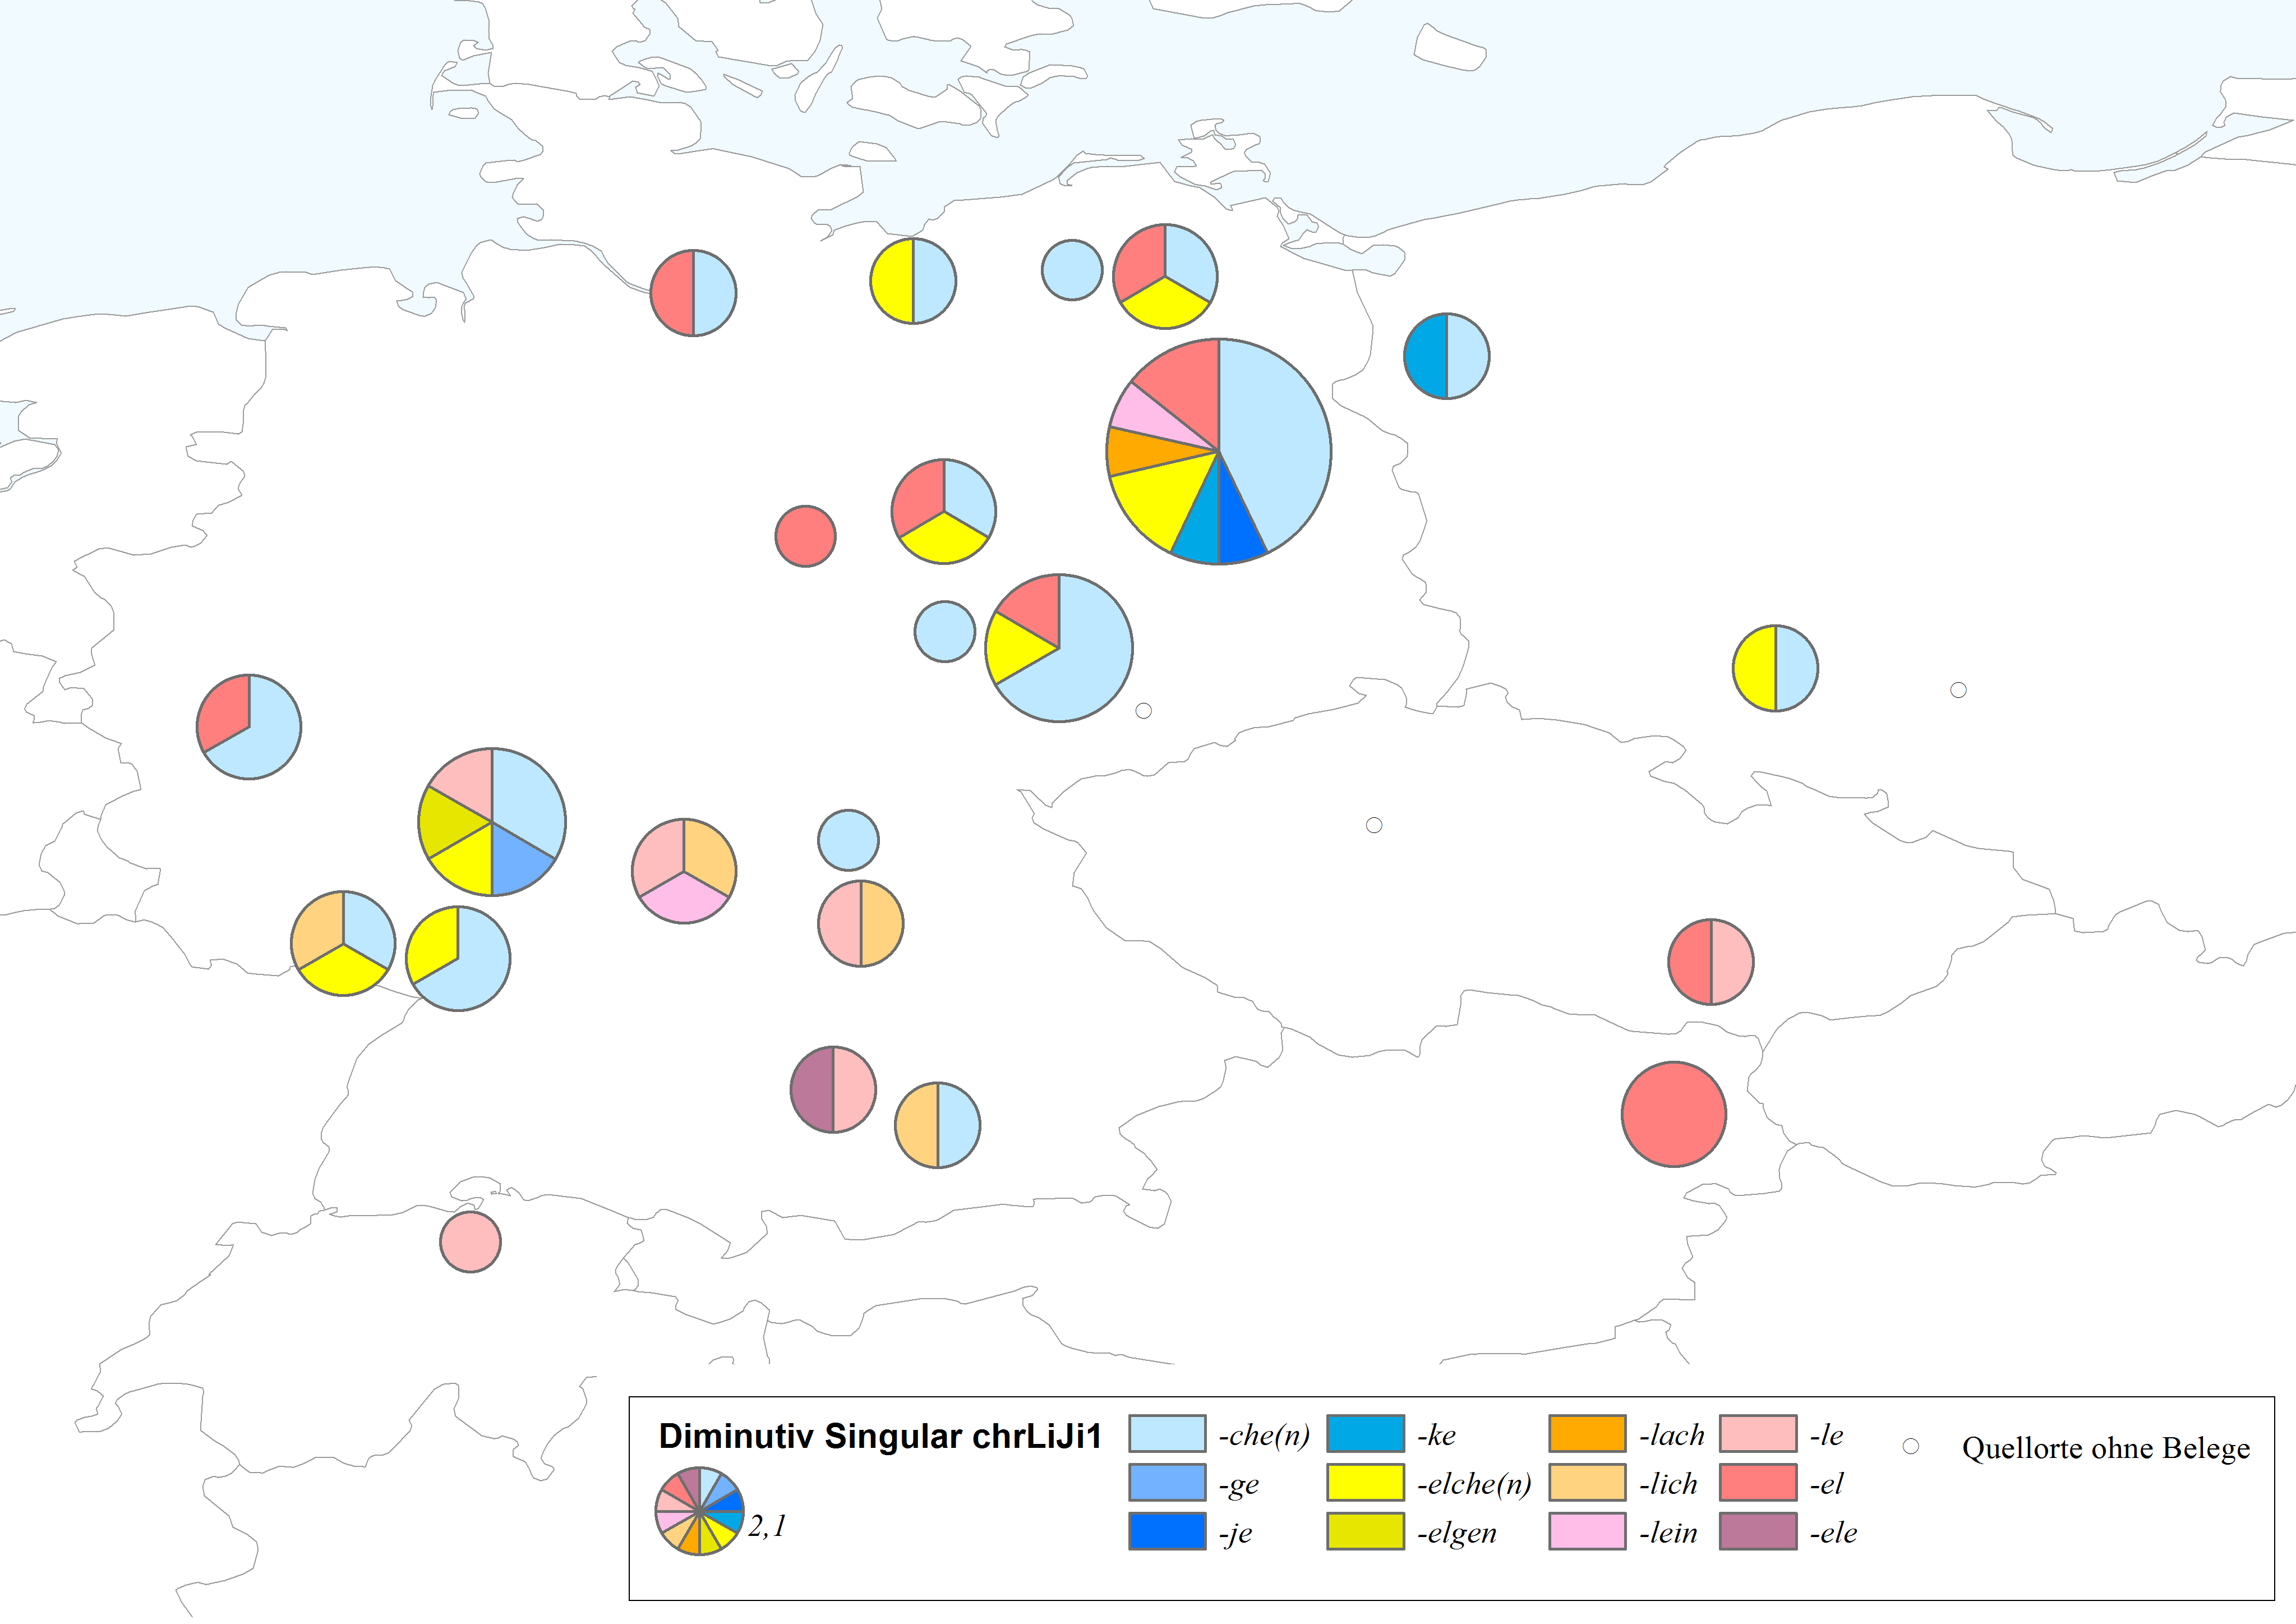
\includegraphics[width=\textwidth]{figures/DIM_SG.png}
		\caption{\label{SgDimliji} Singulardiminutionen im \hai{chrLiJi1}}
		\end{figure} 
 

\begin{figure} 

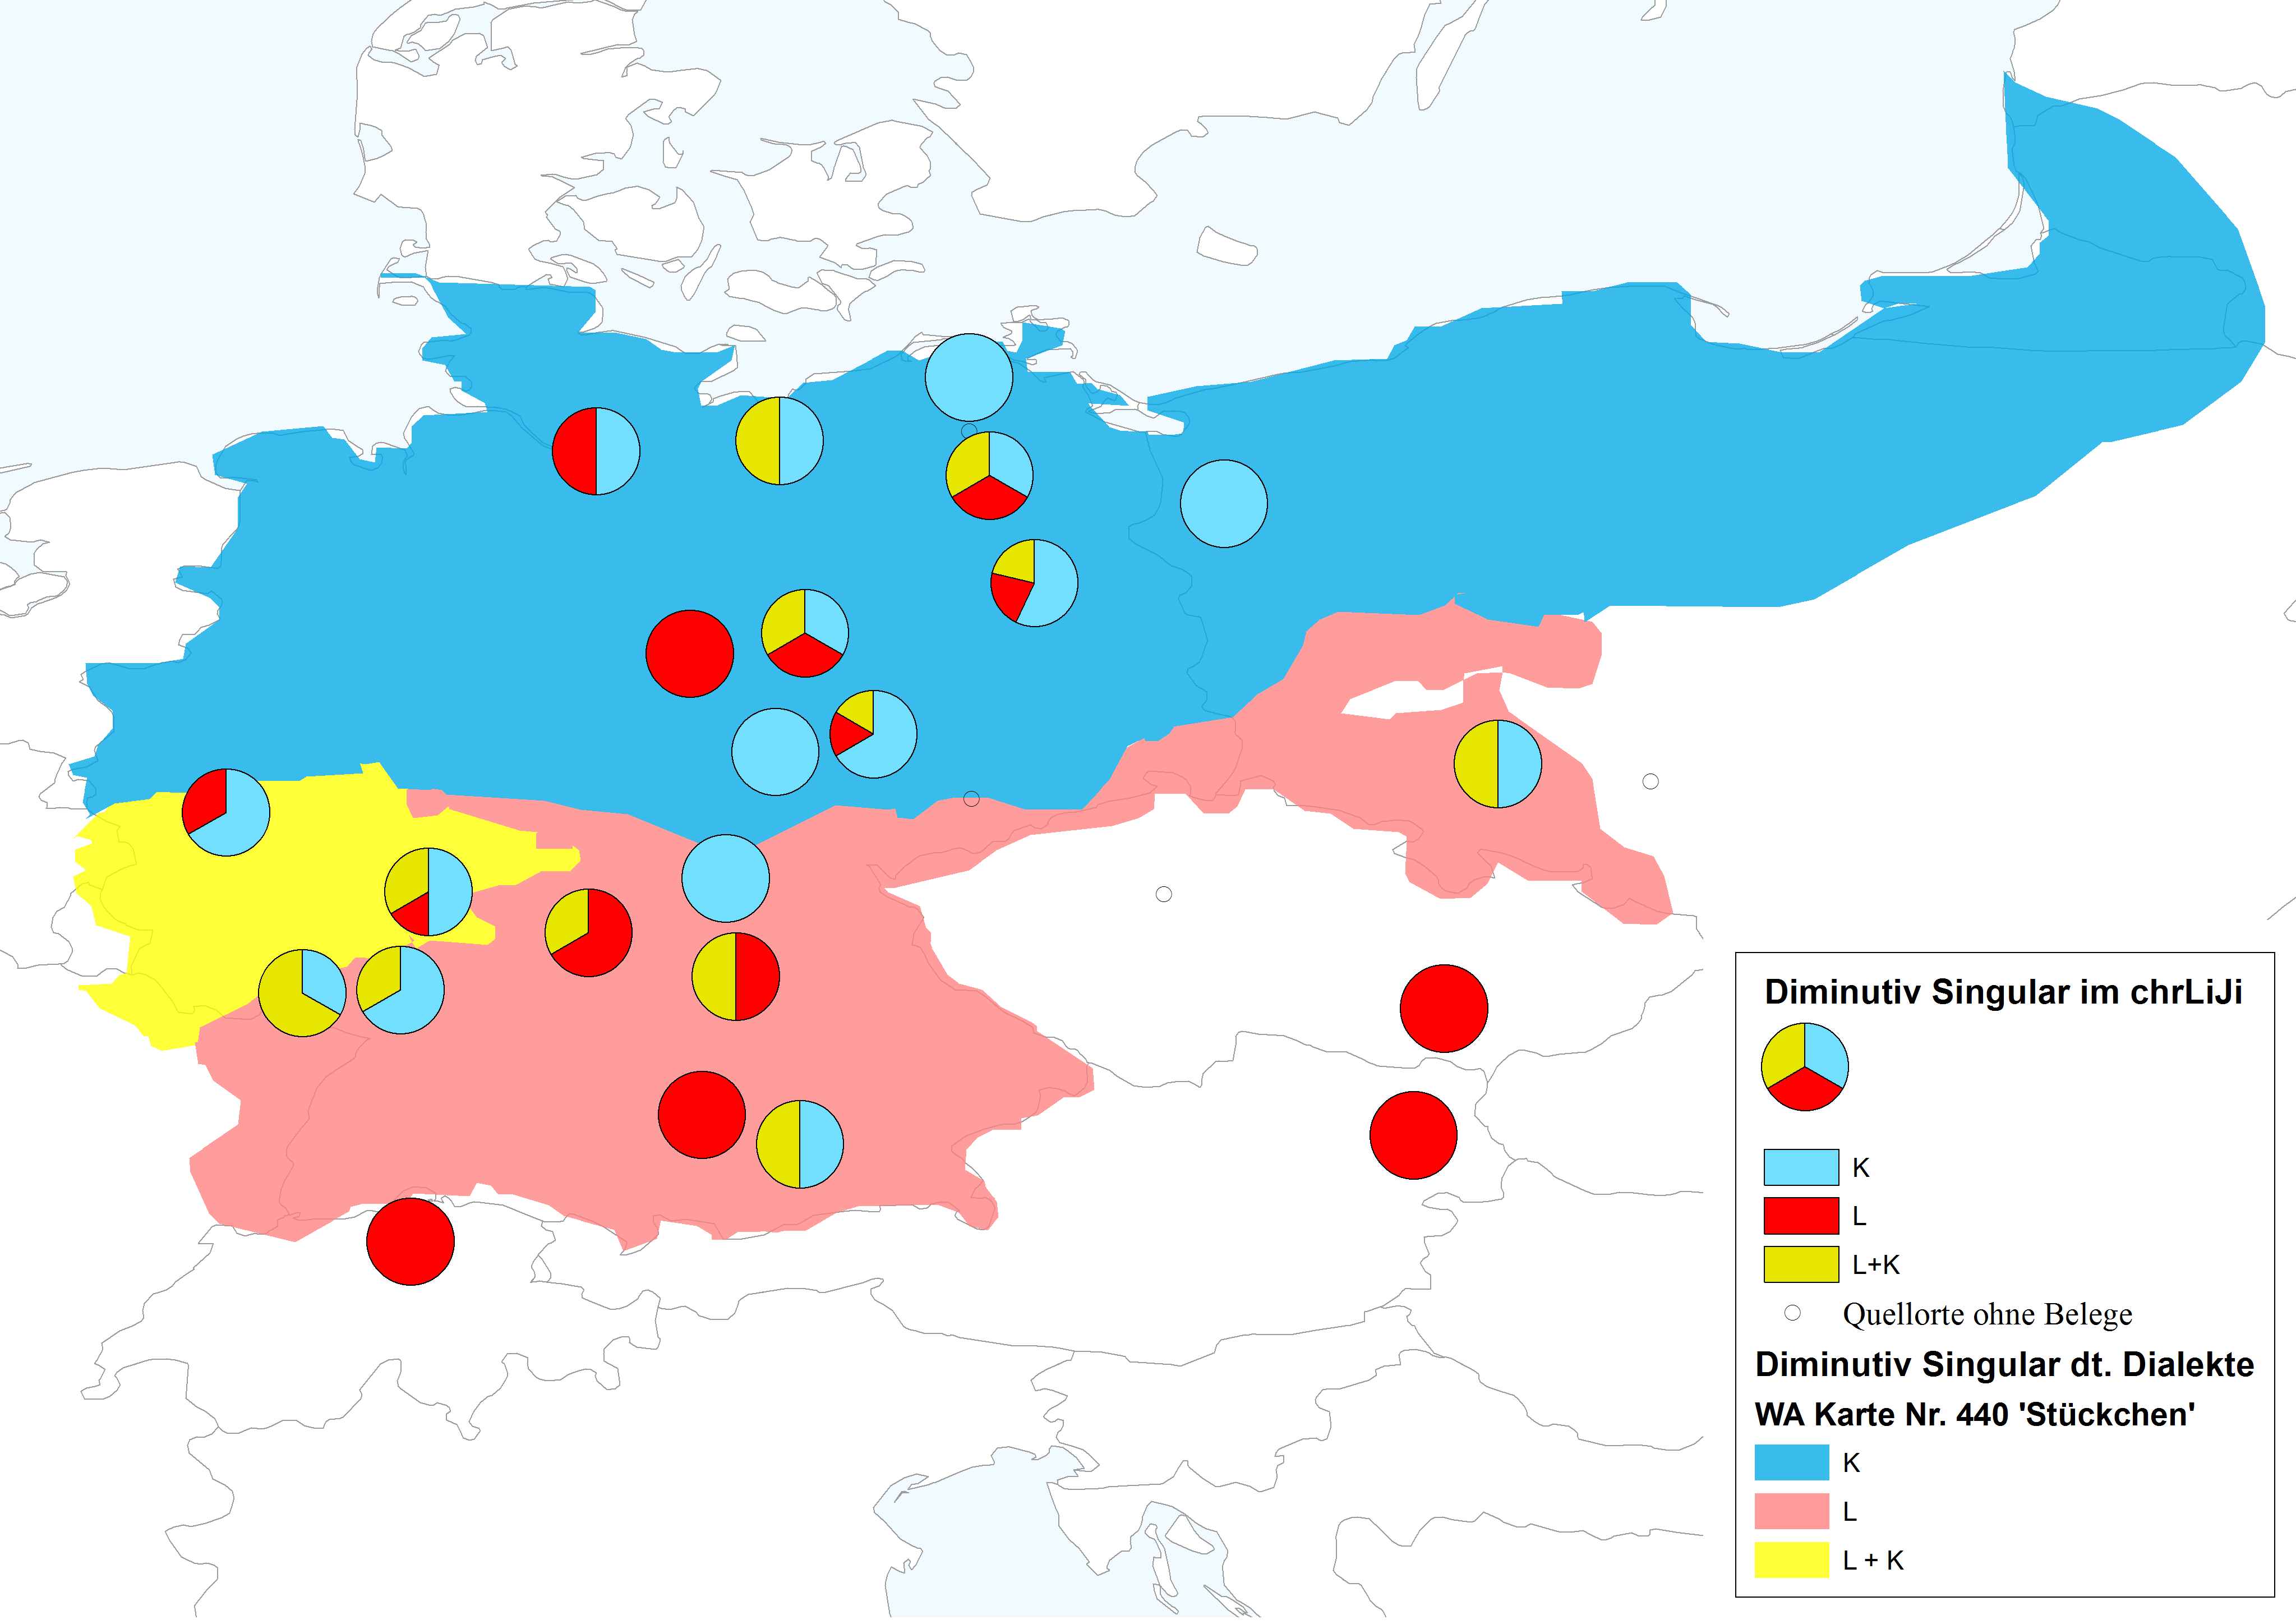
\includegraphics[width=\textwidth]{figures/DIM_SG_DSA_DIM_SG_kurz.png}
		\caption{\label{SgDimDSAliji} Singulardiminutionen im \hai{chrLiJi1} und den dt. Dialekten (\hai{WA} Karte Nr. 440 \sem{Stückchen}) }
		\end{figure}
 
Vier Quellen zeigen das Pluraldiminutivsuffix -\textit{lich} im Singular (s. Abbildung \ref{DimDSALiJilich}, S.\, \pageref{DimDSALiJilich}). Eine solche Verwendung dieses Suffixes im Singular ist weder aus jiddischen noch aus deutschen Varietäten bekannt. Da all diese Quellen das Suffix auch \quein{korrekt} bei der \isi{Diminution} Plural einsetzen, ist anzunehmen, dass es sich hierbei um Übergeneralisierungen handelt.\label{lichHyper} Den meisten Autoren des \hai{chrLiJi1} mag also nicht bewusst gewesen sein, dass das Jiddische eine Unterscheidung zwischen Diminutiv Singular und Plural trifft, und so wurde das  \isi{Pluralsuffix} auf den Singular übertragen.\footnote{Hinzukommt, dass mindestens ein Text durch die Schriften Itzig Veitel Sterns (pseud.) (\hai{GP}  Nürnberg, 1831) beeinflusst ist, welcher -\textit{lich} sowohl im Singular als auch im Plural verwendet; zumindest nennt der Verfasser von \hai{PG} (Speyer, 1835) im Vorwort diesen als sein Vorbild (vgl.\, Abschnitt \ref{IVS}, S.\, \pageref{IVS}).} 
 
Die Kartierung der Daten in den Abbildungen \ref{SgDimliji} und \ref{SgDimDSAliji} zeigt, dass \hai{L}-{Di\-mi\-nu\-tion} über das gesamte Erhebungsgebiet verteilt vorliegt, während \hai{K}-Di\-mi\-nu\-tio\-nen im Süden rar sind. Davon ausgehend lässt sich vermuten, dass einigen der Autoren bewusst war, dass die \isi{Diminution} im Jiddischen auf den \hai{L}-Typ aufbaut. Interessant ist außerdem, dass Fusionsformen nach dem Muster \hai{L+K} im gesamten Gebiet (mit Ausnahme des äußersten Südostens) belegt sind, 
\largerpage[-1]
obwohl diese Form eigentlich charakteristisch für die westmitteldeutschen Dialekte ist. Die bislang bekannten Daten zum Westjiddischen sprechen nicht dafür, dass im Singular solche Fusionsformen dort weit verbreitet waren (vgl.\, S.\, \pageref{DIMSGWJ}). Da jedoch generell die Datengrundlage recht dünn ist, was auch dem Umstand geschuldet ist, dass \isi{Diminution} außerhalb des \hai{{\LiJi}} kein besonders frequentes Phänomen ist und die Wahl der einzelnen Suffixe von Wort zu Wort variieren kann, lässt sich nicht mit Bestimmtheit ausschließen, dass das \hai{chrLiJi1} hier eventuell etwas einfängt, was in den authentischen Quellen des Westjiddischen nicht belegt ist, tatsächlich aber Teil der Sprachrealität war. Für die Existenz einer Fusionsform der Singulardiminutionssuffixe im Jiddischen spricht, dass solche Formen auch im Ostjiddischen belegt sind (\citealt[122, Karten Nr. 36S1, 36S2]{Herzog2000};\,%rs + "Nr."
vgl.\, S.\, \pageref{SOJDIM}) und dass ich das Pluraldiminutivsuffix -\textit{lich}/ -\textit{lekh} als aus einer \hai{L}-\hai{K}-Fusion hervorgegangen auffassen.


  
 
 
 

   
% \todo{Ungefüllten Kreissymbole etwas zu weit oben; kann nicht kompilieren, daher nicht überprüfbar}
 



	
\begin{figure}[t]
	\begin{tikzpicture}
		\begin{axis}[only marks, width=0.82\textwidth,height=0.4\textheight,
		legend style={at={(1,1)},xshift=0.2cm, yshift=-0.5cm,anchor=north west,nodes=left},
			%title={Funktionstypen des sp\"aten Westjiddisch},
			xtick={1700, 1725, 1750, 1775, 1800, 1825, 1850, 1875, 1900, 1925, 1950}, ytick=\empty,
			x tick label style={/pgf/number format/1000 sep=}, 
			y tick label style={/pgf/number format/1000 sep=},
			%extra y ticks={456.1, 1022.4},
			%extra y tick labels={{456,1},{1022,4}},
			extra y tick style={grid=major,
				tick label style={, ,}},
				ymin=0.2,
				ymax=6.2,
			ylabel={\hai{L}-Region  \hspace*{5mm} \hai{L + K}-Region  \hspace*{5mm} \hai{K}-Region},
			enlarge x limits=0.03]	
	
			%K-Gebiet
			\addplot [mark=square*, red] table [x=jahr, y=KDIML] {figures/KDIML.txt};%1.4
			\addplot [ultra thick, mark=triangle*, yellow] table [x=jahr, y=KDIMLK] {figures/KDIMLK.txt};%1
			\addplot [mark=o] table [x=jahr, y=KDIMK] {figures/KDIMK.txt};%1.4

 \draw[gray!50] (-0.2cm,4cm) -- (15.5cm,4cm);		
			
			%LK-Gebiet
			\addplot [mark=square*, red] table [x=jahr, y=LKDIML] {figures/LKDIML.txt};%1.4
			\addplot [mark=triangle] table [x=jahr, y=LKDIMLK] {figures/LKDIMLK.txt};%1
			\addplot [mark=*, blue] table [x=jahr, y=LKDIMK] {figures/LKDIMK.txt};%1.4
	 \draw[gray!50] (-0.2cm,2.1cm) -- (15.5cm,2.1cm);		
		
			%L-Gebiet

			\addplot [mark=square] table [x=jahr, y=LDIML] {figures/LDIML.txt};%1.4
			\addplot [ultra thick, mark=triangle*, yellow] table [x=jahr, y=LDIMLK] {figures/LDIMLK.txt};%1
			\addplot [mark=*, blue] table [x=jahr, y=LDIMK] {figures/LDIMK.txt};%1.4


						\legend{\hai{L}-{\Dim}, \hai{LK}-{\Dim}, \hai{K}-{\Dim}, \hai{L}-{\Dim}, \hai{L + K}-{\Dim}, \hai{K}-{\Dim},\hai{L}-{\Dim}, \hai{L + K}-{\Dim}, \hai{K}-{\Dim}} 
		\end{axis}
	\end{tikzpicture}
	\caption{Regionale Verteilung von Singulardiminutionen im \hai{chrLiJi1}}
	\label{REGDIMSG}	
\end{figure}



Die Karten in Abbildung \ref{SgDimliji} und \ref{SgDimDSAliji} ließen die Vermutung zu, dass \hai{L}-Di\-mi\-nu\-tio\-nen durch ostjiddischen Einfluss erst im Verlauf des 19. Jahrhunderts im Norden auftauchen. Das Histogramm in Abbildung \ref{REGDIMSG}, welches die Quellen je nach regionaler Lage im deutschen Diminutionssystem (ausgehend von \hai{WA} Karte Nr. 440) sortiert, zeigt aber, dass wir in der \hai{K}-Region, also im Norden des Untersuchungsgebiets, bereits um 1800 \hai{L}-\isi{Diminution} vorfinden. Ebenso ist \hai{K}-\isi{Diminution} in den älteren Quellen im Süden (\hai{L}-Region) belegt.\label{LKinberlin} Die Fusionsformen \hai{L+K} hingegen zeigen insofern ein areales Muster, als dass wir sie nur in zwei relativ jungen Quellen in der \hai{L}-Region finden, und sie besonders im Norden (\hai{K}-Region) frequent sind. Eine diachrone Entwicklung von Diminutivtypen im \hai{chrLiJi1} ist also nicht festzustellen. Generell zeigen Karten und Diagramm deutlich, dass im Norden (\hai{K}-Region) mehr von der regionalen Variante (in dem Fall auch der schriftsprachlichen Variante) abweichende Variation zu finden ist, als in der (westlichen) Mitte (\hai{L+K}-Region) oder im Süden (\hai{L}-Region). Zu beachten ist, dass sich die meisten Belege der \hai{K}-\isi{Diminution} aus dem schriftsprachlichen Suffix \textit{-chen} ergeben (wenn auch in manchen Fällen mit gesprochensprachlichem \textit{n}-Ausfall) und damit eher als Hintergrundrauschen der Schriftsprache denn als tatsächliche Evidenz für eine literaturjiddische Manipulation zu deuten sind.\footnote{Es wurde darauf verzichtet, ein vergleichbares Diagramm wie jenes in Abbildung \ref{REGDIMSG} für die Pluraldiminution mit anzuführen, da dieses ebenfalls keine Beziehungen zwischen zeitlich-räumlichen Auftreten einer Struktur im \hai{chrLiJi1} aufweist.}\label{sgDIMimNordenmehr} Ebenfalls als Reflex der deutschen Schriftsprache sind Belege für das Suffix \textit{-ge} zu deuten, da dieses Suffix noch bis ins 18. Jahrhundert als \qu{Leitvariante} der \isi{Diminution} galt und im 19. Jahrhundert, wenn auch sukzessive durch \textit{-chen} abgelöst, noch immer gebräuchlich ist (\citealt{Wegera2000b}; \citealt[73f]{Elspass2005}).


		 

 

  
Im Plural zeigt sich hingegen folgendes Bild: 27 Quellen weisen eine \isi{Diminution} eines Plurals auf. Jedoch nur neun der Suffixe zeigen eine eigene morphologische Markierung des Plurals am Diminutivum (vgl.\, Tabelle \ref{tblDIMPL}).\footnote{\label{FNDIMPL}Diese Suffixe sind \textit{-cher}, \textit{-elcher}, \textit{-ercher}, \textit{-elger}, \textit{-chens}, \textit{-ches}, \textit{-ges}, \textit{-els} und \textit{-lich}. Je nach Ansatz ließe sich auch im Suffix -(\textit{ens})\textit{ke} eine Fussion aus \textit{en}-Plural mit \textit{s}-Plural und \hai{K}-\isi{Diminution} erkennen.} In vielen Fällen wird die Pluraldiminution mittels einer Addition des  \textit{-er}- oder \textit{-s}-\isi{Pluralsuffix} mit dem Diminutivsuffix vollzogen. Immerhin sechs Quellen setzen das jiddische Suffix \textit{-lich} ein (vgl.\, Fn. \ref{FNDIMPL}).\footnote{Die Quellen mit dem jiddischen Suffix \textit{-lich} sind: \hai{PG} (Speyer, 1835), \hai{PA} (Frankfurt, 1834), \hai{LM} (Würzburg, 1844), \hai{GP} (Nürnberg, 1831), \hai{SV} (München, 1890) und \hai{DG} (Wien, 1858).} Vier dieser Quellen (\hai{PA} Frankfurt, 1834, \hai{LM} Würzburg, 1844, \hai{GP} (Nürnberg, 1831) und \hai{SV} (München, 1890)) setzen dabei \textit{-lich} auch zur Singulardiminution ein. In diesen Fällen kann man sehr wahrscheinlich von einer Hyperkorrektur des jiddischen Systems ausgehen (vgl.\, S.\, \pageref{lichHyper} u. Karte in Abbildung \ref{DimDSALiJilich}). Doch gibt es tatsächlich in den deutschen Dialekten auch Fälle, in denen Plural- und die Singularform unter -\textit{lich} zusammengefallen sind (z.\,B.\, in den Wenkerbögen von Hohenstraßen 34519, Niederhochstadt 33266, Heiligkreuz 27473). Diese Einzelfälle finden sich bemerkenswerter Weise besonders in Randgebieten der Areale die -\textit{lich}-Pluraldiminution aufweisen. Es ist also nicht gänzlich auszuschließen, das die Singularbelege für -\textit{lich} Singulardiminution im \hai{chrLiJi1} nicht auf die autoreigene Mündlichkeit zurückzuführen sind. Alles in Allem liegt letzten Endes in lediglich zwei Quellen des \hai{chrLiJi1} (\hai{PA} Frankfurt, 1834 u. \hai{DG} Wien, 1858) das tatsächliche jiddische Diminuierungssystem im Plural vor. Auffällig ist auch, dass die Belege zur Pluraldiminution mittels \textit{-lich} in relativer Nähe zu den Gebieten liegen, in denen laut \hai{WA}-Karte(n) dieses Suffix auch in den deutschen Dialekten üblich ist (vgl.\, Abbildung \ref{DimDSALiJilich}). \,%rs + "Abbildung"

 \begin{table}[t]
		\begin{tabularx}{\columnwidth}{lXr}

	\lsptoprule

\textbf{Suffix} &\textbf{Beispiel} & \textbf{Quellen} \\ \midrule 


\textit{-che(n)} & \textit{Diminutivchen} \sem{Diminutiv\textsubscript{{\Dim} {\Pl}}} (\hai{{\PP}}:\,27), \textit{Steinchen} \sem{Stein\textsubscript{{\Dim} {\Pl}}} (\hai{FS}:\,45, 73), \textit{Bäumchen} \sem{Baum\textsubscript{{\Dim} {\Pl}}} (\hai{PS}:\,28, 44) & 10 \\
 
  \textit{-cher} & \textit{Stickcher} \sem{Stück\textsubscript{{\Dim} {\Pl}}} (\hai{PA}:\,8, 17), \textit{Köpfcher} \sem{Kopf\textsubscript{{\Dim} {\Pl}}} (\hai{BS}:\,7),   \textit{Mädcher} \sem{Mädchen\textsubscript{{\Dim} {\Pl}}} (\hai{PL}:\,39, 50) & 6\\
 
  \textit{-chens} & \textit{Beinchens} \sem{Bein\textsubscript{{\Dim} {\Pl}}} (\hai{{\PP}}:\,20), \textit{Mäuschens} \sem{Maus\textsubscript{{\Dim} {\Pl}}} (\hai{BW} Leipzig, 1826:\,108) & 4 \\
 
  \textit{-ches} & \textit{Semmelches} \sem{Brötchen\textsubscript{{\Dim} {\Pl}}} (\hai{BW} Leipzig, 1826:\,99, 105, 110), \textit{Banches } \sem{Bein\textsubscript{{\Dim} {\Pl}}} (\hai{PG}:\,44), \textit{Sternches} \sem{Stern\textsubscript{{\Dim} {\Pl}}} (\hai{JK}:\,11)& 5 \\
 
  \textit{-(ens)-ke} & \textit{Soldatenske} \sem{Soldat\textsubscript{{\Dim} {\Pl}}} (\hai{AJ}:\,1) & 1\\
 
  \textit{-ges} & \textit{Gesellschaftges} \sem{Gesellschaft\textsubscript{{\Dim} {\Pl}}} (\hai{PA}:\,23) & 1\\
 
 
  \textit{-elcher} & \textit{Stickelcher} \sem{Stück\textsubscript{{\Dim} {\Pl}}} (\hai{VD}:\,17), \textit{Jüngelcher} \sem{Junge\textsubscript{{\Dim} {\Pl}}} (\hai{PG}:\,17, 18, 19) & 2 \\
 
  \textit{-ercher} & \textit{Kindercher} \sem{Kind\textsubscript{{\Dim} {\Pl}}} (\hai{PG}:\,39, 43) & 1 \\
 
  \textit{-elger} & \textit{Schickselger} \sem{Nichtjüdin\textsubscript{{\Dim} {\Pl}}} (\hai{JK}:\,13), \textit{Jüngelger} \sem{Junge\textsubscript{{\Dim} {\Pl}}} (\hai{OF}:\,2) & 2 \\
 
  \textit{-lich} & \textit{Rädlich} \sem{Rad\textsubscript{{\Dim} {\Pl}}} (\hai{DG}:\,12), \textit{Büchlich} \sem{Buch\textsubscript{{\Dim} {\Pl}}} (\hai{SV}:\,V), \textit{Gänslich} \sem{Gans\textsubscript{{\Dim} {\Pl}}} (\hai{LM}:\,27)& 6\\
 
   \textit{-lein} & \textit{Äugelein} \sem{Auge\textsubscript{{\Dim} {\Pl}}} (\hai{LM}:\,27), \textit{Kindelein} \sem{Kind\textsubscript{{\Dim} {\Pl}}} (\hai{WA}:\,157) & 1 \\
  
         \textit{-el} & \textit{Schicksel} \sem{Nichtjüdin\textsubscript{{\Dim} {\Pl}}} (\hai{MV}:\,61) & 1 \\
    
        
    \textit{-els} & \textit{Schicksels} \sem{Nichtjüdin\textsubscript{{\Dim} {\Pl}}} (\hai{JP}:\,44) & 1 \\

 
 
\lspbottomrule
 \end{tabularx}
		 \caption{Diminutivsuffixe Plural im \hai{chrLiJi1}}
		 \label{tblDIMPL}
		 \end{table}

  
   Damit ist nicht auszuschließen, dass dies eine Rolle bei den Imitationen gespielt hat. Zumindest ist es möglich, dass die Nähe zur deutschen Form die korrekte Verwendung der jiddischen Form erleichtert hat. 

\newpage 
Die Daten zur \isi{Diminution} im \hai{chrLiJi1} zeigen je nach Numerus unterschiedliche Raumstrukturen. Die nördlichen Quellen im \hai{K}-Gebiet sind, was die Singulardiminution betrifft, vielfältiger als der Süden oder die westliche Mitte (vgl.\, S.\, \pageref{sgDIMimNordenmehr}). Im Plural hingegen zeigen der Süden und die Mitte mehr Belege für eine gesonderte Pluralmarkierung am Diminutivsuffix als der Norden (vgl.\, Abbildung \ref{Dimliji}).

  
  
  
   
   \begin{figure} 

\includegraphics[width=\textwidth]{figures/DIM_PL.png}
		\caption{\label{Dimliji} Pluraldiminutionen im \hai{chrLiJi1} (Einzelsuffixe)}
		\end{figure}  
  
  
  
  \begin{figure} 

\includegraphics[width=\textwidth]{figures/DIM_PL_kurz.png}
		\caption{\label{Dimlijikurz} Pluraldiminutionen im \hai{chrLiJi1} (Grundmuster)}
		\end{figure}  
  
   
 
 
  
 


  \begin{figure} 

\includegraphics[width=\textwidth]{figures/DIM_PL_DSA_Kurz.png}
		\caption{\label{DimDSALiJi} Pluraldiminutionen im \hai{chrLiJi1} und den dt. Dialekten (\hai{WA} Karte Nr. 381 \sem{Apfelbäumchen})}
		\end{figure}  
 



\begin{figure} 

\includegraphics[width=\textwidth]{figures/lich_Dim_pl_sg_DSA.png}
		\caption{\label{DimDSALiJilich} -\textit{lich}-Diminutionen im \hai{chrLiJi1} und den dt. Dialekten (\hai{WA} Karte Nr. 381 \sem{Apfelbäumchen})}
		\end{figure}
  
\newpage 
\subsection{Diminution im \hai{jüdLiJi1} }\label{DIMjüdLiJi1}
%  %\noindent 
Auch im \hai{jüdLiJi1} findet sich eine Vielzahl an Diminutionen. Diese sind in allen der zehn untersuchten Texte belegt. Die Quellen aus Berlin (\hai{GuS1–23}, \hai{PBerlin1–2}) zeigen im Singular wie im Plural allesamt das schriftsprachliche Suffix \textit{-che(n)} (vgl.\, Tabelle \ref{tblDIMjüdliji1SG}). Die südlicheren Quellen verwenden hingegen \hai{L}-Diminutionen. Nur im Fall von \hai{PBreslau} finden sich alle drei Diminutionstypen (\hai{K}, \hai{L}, \hai{L + K}) parallel. 


  \begin{table}
		\begin{tabularx}{\columnwidth}{lXr}
\lsptoprule
\textbf{Suffix} &\textbf{Beispiel} & \textbf{Quellen} \\ \midrule 

\textit{-che(n)} & \textit{Lokomotivche} \sem{Lokomotive\textsubscript{{\Dim} {\Sg}}} (\hai{GuS1}:\,5), \textit{Liedche} \sem{Lied\textsubscript{{\Dim} {\Sg}}} (\hai{GuS5}:\,9), \textit{Geschäftchen} \sem{Geschäft\textsubscript{{\Dim} {\Sg}}}  (\hai{GuS23}:\,12), \textit{Demonschtratziönche} \sem{Demonstration\textsubscript{{\Dim} {\Sg}}} (\hai{PBerlin2}:\, 2.\,Sp.), \textit{Wörtche} \sem{Wort\textsubscript{{\Dim} {\Sg}}} (\hai{PBerlin1}:\,2) & 8 \\ 

 
 \textit{-elche} & \textit{Jüngelche} \sem{Junge\textsubscript{{\Dim} {\Sg}}} (\hai{PBreslau}:\,339) & 1 \\
 
 \textit{-le} & \textit{Schreibebriefle} \sem{Brief\textsubscript{{\Dim} {\Sg}}} (\hai{PAlsleben}:\,Titel, 3) & 1\\

 \textit{-el}/\textit{-l} & \textit{Päckel} \sem{Packet\textsubscript{{\Dim} {\Sg}}} (\hai{PBreslau}:\,342),  \textit{Stückel} \sem{Stück \textsubscript{{\Dim} {\Sg}}} (\hai{PDebrecen}:\,7, 13) & 2 \\
 
 \textit{-ele} & \textit{Büchele} \sem{Buch\textsubscript{{\Dim} {\Sg}}} (\hai{PDebrecen}:\,9),  \textit{Haisele} \sem{Hase \textsubscript{{\Dim} {\Sg}}} (\hai{PDebrecen}:\,13) & 1 \\ 
 
     \lspbottomrule
 \end{tabularx}
		 \caption{Diminutivsuffixe Singular im \hai{jüdLiJi1}}
		 \label{tblDIMjüdliji1SG}
		 \end{table}


  \begin{table}
		\begin{tabularx}{\columnwidth}{lXr}

	\lsptoprule

\textbf{Suffix} &\textbf{Beispiel} & \textbf{Quellen} \\ \midrule 
  \textit{-cher} & \textit{Ameischer} \sem{Ameise\textsubscript{{\Dim} {\Pl}}} (\hai{GuS1}:\,3),  \textit{Perzentcher} \sem{Prozent\textsubscript{{\Dim} {\Pl}}} (\hai{GuS5}:\,7),  \textit{Schwebelhölzcher} \sem{Schwefelholz\textsubscript{{\Dim} {\Pl}}} (\hai{GuS10}:\,5), \textit{Tröppcher} \sem{Tropfen\textsubscript{{\Dim} {\Pl}}} (\hai{PBerlin1}:\,2)  & 4 \\

  \textit{-che(n)} & \textit{Kreppchen} \sem{Krapfen\textsubscript{{\Dim} {\Pl}}} (\hai{GuS15}:\,3), \textit{Bettchen} \sem{Bet\textsubscript{{\Dim} {\Pl}}} (\hai{PBerlin1}:\,2), \textit{Affzierche} \sem{Offizier\textsubscript{{\Dim} {\Pl}}} (\hai{PBerlin2}:\,1.\,Sp.) & 3 \\

 
  \textit{-chers} & \textit{Offißierchers} \sem{Offizier\textsubscript{{\Dim} {\Pl}}} (\hai{PBerlin2}:\,2.\,Sp.) & 1 \\
 
 
  \textit{-ercher} & \textit{Gesetzercher} \sem{Gesetz\textsubscript{{\Dim} {\Pl}}} (\hai{PBerlin1}:\,4) & 1 \\
 
   \textit{-che(n)s} & \textit{Bäckches} \sem{Backe\textsubscript{{\Dim} {\Pl}}} (\hai{PBerlin1}:\,2), \textit{Kupperhütchens} \sem{Kupferhut\textsubscript{{\Dim} {\Pl}}} (\hai{GuS10}:\,10) & 3 \\
   
   \textit{-lech} & \textit{Jidlech} \sem{Jude\textsubscript{{\Dim} {\Pl}}} (\hai{PDebrecen}:\,7),  \textit{Zeitungblättlech} \sem{Zeitungsblatt\textsubscript{{\Dim} {\Pl}}} (\hai{PDebrecen}:\,14)  & 1 \\
  
\lspbottomrule
 \end{tabularx}
		 \caption{Diminutivsuffixe Plural im \hai{jüdLiJi1}}
		 \label{tblDIMjüdliji1PL}
		 \end{table}

 
    
    Besonders authentisch bezüglich der \isi{Diminution} präsentiert sich \hai{PDebrecen}, wo wir den einzigen Beleg einer Pluraldiminution mittels \textit{-lech} finden. Bemerkenswert daran ist, dass wir hier bereits die ostjiddische Vokalisierung des Suffixes antreffen und nicht die westjiddische (\textit{-lich}), wie sie im \hai{chrLiJi1} belegt ist. In den \hai{GuS1–10} finden wir ausschließlich die Pluralsuffixe \textit{-cher} und \textit{-chen} (vgl.\, Tabelle \ref{tblDIMjüdliji1PL}). Eine besondere Vielfalt an Diminutionssuffixen im Plural findet sich in \hai{PBerlin1} (\textit{-chen}, \textit{-ches}, \textit{-ercher}, \textit{-chers}) und \hai{PBerlin2} (\textit{-che}, \textit{-ches}, \textit{-chens}). Diese Suffixe funktionieren nach dem Prinzip \hai{K}+\hai{{\Pl}} (bzw. in einem Fall \hai{{\Pl}}+\hai{K}+\hai{{\Pl}}) und bauen damit auf die \hai{K}-\isi{Diminution} auf. Es findet sich, vom \textit{-lech}-Beleg aus \hai{PDebrecen} abgesehen, kein einziger Beleg für Pluraldiminutiva der Fusionsformen, wie wir sie im \hai{chrLiJi1} besonders im Nordosten finden (vgl.\, S.\, \pageref{LKinberlin}). Hierin besteht also ein deutlicher Unterschied zwischen \hai{chrLiJi1} und \hai{jüdLiJi1}. 

Zusammenfassend lässt sich feststellen, dass im \hai{jüdLiJi1} weniger Aufwand betrieben wurde, Suffixe zu wählen, die nicht der örtlichen deutschen \isi{Diminution} entsprechen, als es im \hai{chrLiJi1} der Fall ist. Das Besondere an den Belegen zur \isi{Diminution} im \hai{jüdLiJi1} ist, dass diese vergleichbar hoch frequent sind wie im \hai{chrLiJi1}. Es ist also vielmehr die reine Präsenz von \isi{Diminution} als deren konkrete morphologische Struktur, die die Gemeinsamkeit beider Formen des \hai{{\LiJieins}} ausmacht. Diminutive können durch die ironische, scherzhafte Funktion des \hai{C2}-Typs provoziert sein und wären damit textsortenspezifisch. Mit Blick auf die Situation im \hai{chrLiJi1} liegt es jedoch nahe, \isi{Diminution} als figurenspezifisch \quein{jüdisch} anzusehen. Darüber hinaus bestärken die Belege aus dem \hai{jüdLiJi1} die Vermutung, dass die Diminutionsmorphologie (insbes. Singulardiminution) im Westjiddischen vielfältig ist und kleinräumige regionale Muster anzunehmen sind. Doch für weitere Ergebnisse dieser Art ist das \isi{Korpus} zum \hai{jüdLiJi1} zu klein und die geographische Streuung der Quellen (auch die aller potenzieller Quellen) zu gering.

 \subsection{Funktionen von Diminution im \hai{{\LiJi}} }\label{DIMFunktionen}
%  %\noindent
   Die Funktion der Diminutivsuffixe im \hai{chrLiJi1} ist schwer auszumachen. Zum einen ist es möglich, dass mit ihnen  eine tatsächliche Sprachrealität abgebildet wird, die aufgrund der dünnen Quellenlage nicht klar umrissen werden kann, zum anderen aber sind die Formen areal und diachron zu wahllos verbreitet, als dass dies Rückschlüsse auf feinere Strukturen zuließe. Was grobe Raumstrukturen betrifft, so bieten die Daten des \hai{chrLiJi1} immerhin Ansätze für weitere Untersuchungen. Durch authentische Quellen zu prüfen wären besonders die Hypothesen, dass \hai{L+K}-Fusionsformen im Singular im Nordosten des Westjiddischen verbreitet waren oder dass die Pluraldiminution mittels -\textit{lich} lediglich im Süden des Sprachgebiets tatsächlich verwendet wurde, während im Norden andere, auf \hai{K}-Diminutionen aufbauende Formen, präsent waren.


Die Analyse hat gezeigt, dass sich die Quellen des \hai{jüdLiJi1}  ähnlich den koterritorialen Quellen des \hai{chrLiJi1} verhalten. Andererseits irritiert besonders, dass wir im \hai{chrLiJi1} eine solch große Variation an Suffixen vorfinden, die uns aus den jiddischen Varietäten nicht bekannt ist (vgl.\, Abschnitt \ref{dimJIDDISCH}) und auch nicht durch Daten des \hai{jüdLiJi1} bestätigt wird. Hinzu kommt, dass sich \isi{Diminution} außerhalb des \hai{{\LiJi}} als Charakteristikum der jiddischen Sprache etabliert haben muss, anders ist nicht zu erklären, warum sie bereits vielfach in den frühesten Quellen belegt ist (vgl.\, Abbildung \ref{REGDIMSG}). Dies spricht dafür, anzunehmen, dass \isi{Diminution} an sich, also unabhängig der morphologischen Struktur des Suffixes, besonders stark als grammatische Kennfunktion \textit{jüdischer Sprache} agiert. Um ein besseres Bild der Funktionen von \isi{Diminution} im \hai{{\LiJi}} zu gewinnen, bedarf es allerdings weiterer Daten der gesprochenen und geschriebenen Sprache. Erst dann könnte geklärt werden, ob ein äußerst hoher Gebrauch an Diminutiva tatsächlich der jiddischen Sprachrealität entspricht oder nicht. 

 \section{Plurale}\label{pl}
 %\noindent

\largerpage[-1]
In einigen Fällen weist das \hai{{\LiJi}} Pluralformen auf, die vom Schriftdeutschen abweichen. Besonders populär ist dabei die Verwendung des  \textit{s}-Plurals (vgl.\, Unterabschnitte S.\, \pageref{sPlural} u. S.\, \pageref{sPluralLiJi}). Eine weitere, jedoch deutlich seltener auftretende Pluralmorphemalternanz wird in Unterabschnitt \ref{erPLURAL} vorgestellt. Bevor auf die Daten zum \hai{{\LiJi}} näher eingegangen wird, gibt der nachfolgende Unterabschnitt \ref{plDEUJI} einen allgemeinen Überblick zu den Grundmustern der Pluralbildung im Jiddischen und Deutschen.


 
\subsection{Grundmuster der Pluralmorphologie im Jiddischen und Deutschen}\label{plDEUJI}
%  %\noindent 
 Das Pluralsystem
%  in den deutschen Dialekten 
der deutschen Dialekte ist alles andere als einheitlich. Nicht nur, dass dialektale Variation bei der Wahl der Pluralisierungsstrategie vorliegt, sondern es gibt  in den Dialekten  Strategien, wie z.\,B.\, Pluralmarkierung durch \isi{Subtraktion} (vgl.\, \citealt{GolstonWiese1996,HolsingerHouseman1999,Knaus2003,BirkenesDiss}), die die Schriftsprache nicht kennt (vgl.\, \citealt[414–443]{Schirmunski1962}; \citealt{Nuebling2005}; \citealt[insbes. 155–169]{Wiese2009}). Pluralisierung im Jiddischen folgt in den meisten Fällen Strategien, die auf die germanische Komponente zurückgehen. Der Plural wird überwiegend nach den folgenden Prinzipien gebildet: -\textit{er}, -\textit{(e)n}, -\textit{∅},  -\textit{(e)s},\footnote{Ob sich die Existenz eines \textit{s}-Plurals im Jiddischen auf die alt- bzw. mittelhochdeutsche Komponente zurückführen lässt, ist anzweifelbar (vgl.\, etwa \citealt{King1990,Timm2007}). Da dies eine Strategie ist, die germanischen Sprachen an sich nicht fremd ist. Denn selbst wenn der \textit{s}-Plural im Jiddischen nicht genuin deutschen Ursprungs ist, so wird das germanische Grundgerüst des Jiddischen, welches einen alt-/\,mittelhochdeutschen Ur\-sprung hat, die Aufnahme dieses Plurals begünstigt und katalysiert haben. Weiter ist zu sagen, dass der einfache -\textit{e}-Plural ± \isi{Umlaut} im Jiddischen durch die \isi{Apokope} abgebaut wurde (\citealt[29]{Timm2007}).\label{FNsplural}} ± \isi{Umlaut} (\ref{PLji1erUmlaut}–\ref{PLji1nurUmlaut} zitiert n. \citealt[163]{Jacobs2005}). Hinzu kommt die aus der \ili{hebräisch}-aramäischen Komponente stammende Pluralbildung mittels  -\textit{im}/ -\textit{em}, die überwiegend auf Lexeme dieser Komponente angewendet wird (\ref{PLji1Hebr} zitiert n. \citealt[165]{Jacobs2005}) und nur in wenigen Ausnahmefällen Lexeme anderer Komponenten betrifft (\ref{PLji1Hebrgerm} zitiert n. \citealt[165]{Jacobs2005}). 
 Wie bereits gezeigt, verfügt das Jiddische über eine gesonderte Pluralbildung im Rahmen der \isi{Diminution} (vgl.\, Abschnitt \ref{dim}).

Wie in den deutschen Dialekten, so gibt es auch in den jiddischen Dialekten areale Variation (\ref{PLji1dialekt}). Zur Situation in den westjiddischen Dialekten fehlt es noch an Detailanalysen, es ist aber anzunehmen,  dass dort ebenso wie in den deutschen und ostjiddischen Dialekten diatopische Variation zu erwarten ist, welche u.\,U. sogar parallel zu denen der deutschen Dialekte liegt. So finden wir etwa in einer unserer ältesten Quellen des gesprochenen Westjiddischen, der \qu{Hochzeit zu Grobsdorf}, bereits  Belege für Interferenzen mit den örtlichen hessischen Dialekten, wo der \textit{-er}-Plural besonders \isi{produktiv} ist (s. \ref{PLWJgrob};vgl.\, \citealt[83]{Friebertshaeuser1987}). %rs + "s. Bsp. "

\newpage 

 \eenumsentence{
 \item {\Sg} \RL{לא\makebox(-1.5,-7.5)[r]{\libertineGlyph{uni207B}}נד} \textit{land} \sem{Land} – {\Pl} \RL{לענדער} \textit{lender} \sem{Länder} \label{PLji1erUmlaut} 
 \item {\Sg} \RL{וו{יי}\makebox(-1.5,-3.5)[r]{\libertineGlyph{uni207B}}ב} \textit{vayb} \sem{Weib, Frau} – {\Pl} \RL{וו{יי}\makebox(-1.5,-7.5)[r]{\libertineGlyph{uni207B}}בער} \textit{vayber} \sem{Weiber, Frauen} \label{PLji1nurer}
 \item {\Sg} \RL{ט{יי}\makebox(-1.5,-3.5)[r]{\libertineGlyph{uni207B}}ך} \textit{taykh} \sem{Fluss} – {\Pl} \RL{ט{יי}\makebox(-1.5,-7.5)[r]{\libertineGlyph{uni207B}}כן} \textit{taykhn} \sem{Flüsse} \label{PLji1n} 
  \item {\Sg} \RL{זינגער} \textit{zinger} \sem{Sänger} – {\Pl} \RL{זינגערס} \textit{zingers} \sem{Sänger} \label{PLji1s} 
 \item {\Sg} \RL{הא\makebox(-1.5,-7.5)[r]{\libertineGlyph{uni207B}}נט} \textit{hant} \sem{Hand} – {\Pl} \RL{הענט} \textit{hent} \sem{Hände} \label{PLji1nurUmlaut}
 \item {\Sg} \RL{למדן} \textit{lamdn} \sem{Gelehrter} – {\Pl} \RL{למדים} \textit{lomdem} \sem{Gelehrte} \label{PLji1Hebr}  
  \item {\Sg} \RL{ד{א\makebox(-1.25,-1.25)[r]{\libertineGlyph{uni05B8}}}קטער} \textit{dokter} \sem{Arzt} – {\Pl} \RL{ד{א\makebox(-1.25,-1.25)[r]{\libertineGlyph{uni05B8}}}קטוירים} \textit{doktoyrim} \sem{Ärzte} \label{PLji1Hebrgerm} 
 \item Standard {\oj} u. \hai{{\NOJ}}: {\Sg} \RL{נ{א\makebox(-1.25,-1.25)[r]{\libertineGlyph{uni05B8}}}ז} \textit{noz} \sem{Nase} – {\Pl}  \RL{נעזער} \textit{nezer};\\
 \hai{{\ZOJ}}: {\Sg} \RL{נ{א\makebox(-1.25,-1.25)[r]{\libertineGlyph{uni05B8}}}ז} \textit{noz} \sem{Nase} –  {\Pl} \RL{נייז} \textit{neyz};\\
 \hai{{\SÜJ}} {\Sg} \RL{נ{א\makebox(-1.25,-1.25)[r]{\libertineGlyph{uni05B8}}}ז} \textit{noz} \sem{Nase} –  {\Pl} \RL{נ{א\makebox(-1.25,-1.25)[r]{\libertineGlyph{uni05B8}}}זן} \textit{nozn} \sem{Nasen}\\
 (Bsp. zitiert n. \citealt{Weinreich1960b};\citeyear[9–11]{Weinreich1962})\label{PLji1dialekt} 
    \item {\Sg} \RL{סלו{פ\makebox(-1,4)[r]{\libertineGlyph{afii57807}}}} \textit{slup} \sem{Pfahl} – {\Pl} \RL{סלו{פ\makebox(-1,4)[r]{\libertineGlyph{afii57807}}}ס} \textit{slups} \sem{Pfähle} \label{PLji1sslav} 
    \item {\Pl} \RL{מענשער} \textit{mensher} \sem{Menschen} (\qu{Die Hochzeit zu Grobsdorf} 1822:\,33) \label{PLWJgrob}    
 }
 
 
 %\subsection{Der \textit{s}-Plural im Jiddischen und Deutschen} %ls zusammengefasst mit vorangegangener subsection
 
 %  %\noindent
 Ein besonders umstrittenes Thema in der Germanistik und Jiddistik ist die Genealogie des \textit{s}-Plurals (vgl.\, Fn. \ref{FNsplural}).\label{sPlural} Die Pluralbildung mittels der Suffigierung des Konsonanten \textit{s} ist in vielen modernen romanischen und germanischen Sprachen zu finden. Neben Deutsch und Jiddisch haben z.\,B.\, Französisch, Spanisch, Portugiesisch, Englisch, Niederländisch (und die niederdt. Dialekte), Afrikaans, (West-)Friesisch und  festlandskandinavische Sprachen ein \isi{Pluralsuffix} \textit{-s}; hingegen nicht zu finden \,%rs - ","
 ist es im Isländischen, Färöischen, Italienischen oder Rumänischen\footnote{Im Lateinischen gibt es allerdings Plurale auf -s.} (vgl.\, \citealt{NueblingSchmuck2010}; \citealt[88]{Hoekstra2001}). Obwohl dieser Konsonant damit als Pluralmarker im \quein{Europäischen Sprachbund} sehr weit verbreitet ist, unterscheiden sich die einzelnen Sprachen 
deutlich sowohl im synchronen Gebrauch als auch in den diachronen Entwicklungen zu stark voneinander, als dass ein gemeinsamer Ursprung klar erkennbar wäre. Generell sind Plurale auf \textit{-s} ein eher junges Phänomen der romanischen und germanischen Sprachen und es tritt in den meisten Sprachen zwischen dem 9. und 15. Jahrhundert erstmals in Erscheinung (vgl.\, \citealt{NueblingSchmuck2010}). Es ist gut möglich, dass die \textit{s}-Plurale in den europäischen Sprachen unabhängig voneinander durch internen Sprachwandel entstanden sind und dieser Konsonant aus phonologischen Gründen in diesen Sprachen eine leichte Strategie zur Pluralbildung problematischer Lexeme und untypischer phonologischer Strukturen (wie sie vorwiegend in Fremdwörtern zu finden sind) darstellt (vgl.\, \citealt{Wiese2009}).
 
  
 In den festlandgermanischen Sprachen tritt ein \textit{s}-Plural erstmals im Mittelniederländischen auf (\citealt{NueblingSchmuck2010}; \citealt[422–425]{Schirmunski1962}). Seine Herkunft ist stark umstritten. Manch einer nimmt einen romanischen (altfranzösischen) Einfluss an; andere wiederum sehen den altsächsischen (bzw. altenglischen) \textit{os}/\textit{as}-Plural als Vorbild an (vgl.\, \citealt{Philippa1981, Philippa1982,Oehmann1924}). \,%rs großbuchstabe
 Gegen den französischen Einfluss spricht besonders, dass zum Zeitpunkt des erstmaligen Aufkommens von \textit{s}-Pluralen im Niederländischen (frühes 13. Jahrhundert) dieser im Altfranzösischen selbst noch gar nicht ausgebildet war und nur für Maskulina im \isi{Akkusativ} Plural galt (\citealt[150]{NueblingSchmuck2010}). Und auch ein altsächsischer Einfluss wäre äußerst ungewöhnlich und ist auch besonders problematisch, da eine Überlieferungslücke von \textit{os}/\textit{as}- bzw. \textit{s}-Plural zwischen dem frühen 12. und dem 13. Jahrhundert vorliegt (\citealt[151]{NueblingSchmuck2010}).

 
Während der  \textit{s}-Plural im Niederländischen und Niederdeutschen äußerst \isi{produktiv} wird, ist er für das Hochdeutsche kaum belegt. Erst im Mittelhochdeutschen ist er erstmals bezeugt. Ein französischer Einfluss ist hier weitgehend auszuschließen, u.\,a.\, da er bei französischen Entlehnungen nicht belegt ist und auch nicht besonders frequent in Dialekten entlang der deutsch–\ili{französisch} Sprachgrenze ist, sondern im Gegenteil der \textit{s}-Plural dort kaum üblich ist (\citealt[122–126]{Oehmann1924}). Eine Genese des Mittelhochdeutschen \textit{s}-Plurals aus dem Niederdeutschen ist problematisch, da dieser zwar im Altniederdeutschen noch belegt ist, für das Mittelniederdeutsche, also der Kontaktsprache zum Mittelhochdeutschen, aber nicht bezeugt ist, in den modernen niederdeutschen Dialekten aber hingegen wieder äußerst \isi{produktiv} ist (\citealt[147–150]{Lindowetal1998}). Auch im Frühneuhochdeutschen ist der \textit{s}-Plural noch äußerst selten belegt. Ab 1700 steigen die Belegzahlen besonders bei Lehn- und Fremdwörtern langsam an; in autochthon deutschen Lexemen ist er aber nach wie vor, besonders im niederdeutschen und nördlichen westmitteldeutschen Raum, \,%rs + ,…,
verbreitet (\citealt[266]{Wegera1987}). \,%rs Zitierbefehl fehlte
Ein überzeugendes Szenario für die Herleitung des \textit{s}-Plurals im Gegenwartsdeutsch geht davon aus, dass der \textit{s}-Plural auf das Genitiv-\textit{s} bei \isi{Eigennamen} (insbes. Familiennamen) zurückgeht (\citealt[93]{Wegener2004}; \citealt{NueblingSchmuck2010};vgl.\, \citealt[436f]{Schirmunski1962}).
   
Im gegenwärtigen Hochdeutschen finden wir den \textit{s}-Plural besonders bei Neutra (4,7\% Tokens), selten bei Maskulina (1,4\% Tokens) und äußerst selten bei Feminina (0,2\% Tokens) (\citealt[45–48]{Pavlov1995}). Deutlich häufiger sind Lehn- und Fremdwörter von der Pluralisierung mittels \textit{s} betroffen. \citealt{Wegener2004} zeigt, dass der \textit{s}-Plural hier oft als \quein{Übergangssuffix} fungiert und ein Lexem oft die Deklinationsklasse wechselt sobald es grammatisch integriert ist  (\textit{Pizzas} > \textit{Pizzen}, \textit{Kontos} > \textit{Konten}). Dies ist aber keine Regel und viele Fremdwörter, insbes. gekürzte Fremdwörter, behalten den \textit{s}-Plural (\textit{Autos} > *\textit{Auten}, \textit{Limos} > *\textit{Limen}).
   
 Im modernen Jiddischen ist der \textit{s}-Plural deutlich frequenter als im Deutschen (\citealt{Timm2007}). Er wird z.\,B.\, auf fast alle Maskulina auf -\textit{er}, alle Feminina auf -\textit{in}, viele zweisilbigen Wörter auf -\textit{n}, den überwiegenden Teil aller Substantive der slawischen Komponente (\ref{PLji1sslav} zitiert n. \citealt[163]{Jacobs2005}) und alle auf Vokal ausgehenden Lehnwörter angewandt (\citealt{Timm2007}). Für die diachrone Entwicklung zeigt \cite{Timm2007} drei in (\ref{sPluraljiddischTIMM}) zusammengefasste Phasen auf, 
 in denen sich der \textit{s}-Plural im Jiddischen mehr und mehr ausbreitet. Während \cite[28, 115]{Bin-Nun1973} und \cite{Timm2007} für einen romanischen (Loez) Ursprung des jiddischen \textit{s}-Plurals plädieren (vgl.\, \citealt{Neuberg2007}), sprechen sich \cite[37]{Birnbaum1922}, \cite{King1990}, \cite[399]{Krogh2001} und \cite[402]{Jacobsetal2013} für eine hebräische Genese aus dem Plural für Feminina \RL{ות}- \textit{-ot} und der aschkenasischen Frikativierung von {\hebr} \RL{ת} \textit{t} zu \textit{s} aus. Nur \cite[63–68]{Weinreich1973} verbindet beide Hypothesen und meint, dass sowohl Alt\ili{französisch} als auch Hebräisch dazu beigetragen haben, im Jiddischen den \textit{s}-Plural zu begünstigen. Prinzipiell können alle Argumente, die gegen einen romanischen Ursprung der hoch- und niederdeutschen \textit{s}-Plurale sprechen, auch auf das Jiddische angewandt werden. 
 
  \eenumsentence{
 \item [] \textbf{Phase 1 (11. Jh. – ca.\, 1435):} \textit{s}-Plural in ca.\, 50 Lexemen bezeugt; nicht auf bestimmte Deklinationstypen begrenzt.
 \item [] \textbf{Phase 2 (von 1435–1580):} Zwei Drittel der Belege sind Feminina auf {\mhd} -\textit{in(ne)}. Das restliche Drittel sind Fremd-, Lehnwörter u. Internationalismen.
\item [] \textbf{Phase 3 (seit 1580):} Der \textit{s}-Plural macht die Hälfte aller Pluralbelege aus.
 } \label{sPluraljiddischTIMM}
 

 Der Unterschied zwischen Jiddisch und Deutsch liegt damit nicht nur in der unterschiedlich starken Verwendung des \textit{s}-Plurals, sondern auch in der unterschiedlichen historischen Entwicklung 
dieses Plurals. 
Besonders auffällig ist, dass das Jiddische wesentlich früher als Deutsch einen \textit{s}-Plural etabliert. Mit Blick auf die Stadien \citeauthor{Timm2007}s (\citeyear{Timm2007};
 s. \ref{sPluraljiddischTIMM}) fällt auf, dass besonders während der frühneuhochdeutschen Zeit (1350–1545) der \textit{s}-Plural im Jiddischen einen Zuwachs erfahren hat und systematisiert wurde. In dieser Zeit fanden entscheidende Entwicklung im Jiddischen statt, die es vom Deutschen und seinen Varietäten deutlich entfernte (\citealt{Timm2005,Santorini1992, Santorini1993b, Santorini1993a}). Es ist damit m.\,E. ein durchaus plausibles Szenario, anzunehmen, dass der Unterschied bezüglich der Verwendung und \isi{Frequenz} des \textit{s}-Plurals zwischen 
% modernem 
dem modernen
Deutsch und
%  modernem
dem modernen Jiddisch mit der starken Auseinanderentwicklung beider Varietäten in früh-frühneuhochdeutscher Zeit erklärbar ist (\citealt{Timm2005}). Ein gemeinsamer Ursprung des \textit{s}-Plurals – ggf. im Jiddischen durch den hebräischen Plural zusätzlich begünstigt – wäre damit anzunehmen. Dafür spricht besonders, dass in beiden Sprachen Fremd- und Lehnwörter mittels \textit{s} pluralisiert werden. Die hohe \isi{Frequenz} an \textit{s}-Pluralen bei Nomen der slawischen Komponente spräche für eine funktionale Nähe zum Deutschen, wo dies eine übliche Pluralbildung für Lehn- und Fremdwörter ist (s.\,o.; vgl.\, \citealt{Wegener2004}). 
 
 
 
  \subsection{Der \textit{s}-Plural im Literaturjiddischen}\label{sPluralLiJi}
  %  %\noindent  
  19 Quellen des \hai{chrLiJi1} verwenden einen \textit{s}-Plural, wo er im Schriftdeutschen unüblich ist. Er findet sich im \hai{chrLiJi1} in allen Genera und auch eine Präferenz bestimmter Kasus ist nicht zu erkennen. Eine Quelle (\hai{NW} Berlin, 1804) zeigt ihn in fünf unterschiedlichen Kontexten (\isi{Gallizismus}, \isi{Hebraismus}, \textschwa-Plural, ∅-Plural, \isi{Diminution}); sechs Quellen verwenden das Plural\textit{-s} in je zwei unterschiedlichen Kontexten. Das Gros der Korpustexte (zwölf Quellen) zeigt den \textit{s}-Plural nur in einem morphologischen Kontext. In drei Lexemen findet sich der \textit{s}-Plural an Lexemen, wo er im Standardostjiddischen üblich ist  (s. Tabelle \ref{tblsPLURAL}). Die übrigen Lexeme jedoch werden im Ostjiddischen anders pluralisiert oder gehören erst gar nicht zum ostjiddischen Lexikon (in Tabelle  \ref{tblsPLURAL} markiert als [{\oj} –] ). 
  
  Besonders häufig findet er sich als Fusionssuffix mit Diminutivum (13 Quellen) und  an der Position, wo die deutsche Schriftsprache den ∅-Plural verwendet (6 Quellen inkl. alter Kollektiva). Diminutiva mit \textit{s}-Plural sind in den deutschen Dialekten besonders im niederdeutschen Raum zu finden (Westfälisch, Ostpommersch, Hoch- u. Niederpreußisch; vgl.\, \hai{WA} Karte Nr. 502). Eine Kurzbefragung von Muttersprachlern des Deutschen aus dem Süden und der Mitte ergab jedoch, dass Pluralbildungen mit \textit{-s} am Diminutivsuffix \textit{-chen} durchaus akzeptabel sind. Auch finden sich  Belege dieser Art in der Literatur des 19. und 20. Jahrhunderts wie z.\,B.\, in den Briefen Hugo Balls, der unter keinem niederdt. Einfluss stand: \textit{Und die Blümchens blühen immer noch im Wasserglas} (\citealt[256]{Ball2003}). Der \textit{s}-Plural am Diminutivum ist demnach ein nicht auszuschließendes Phänomen des Deutschen und muss nicht zwangsläufig Teil der sprachlichen Manipulation jüdischer Figurenrede sein. Im \hai{chrLiJi1} finden wir das Plural\textit{-s} jedoch vor allem an Diminutivsuffixen, die nicht der Schriftsprache (\textit{-chen}) entsprechen. Es findet sich in den folgenden Suffixen und Quellen: \textit{-ges} (\hai{PA} Frankfurt, 1834); \mbox{\textit{-els}} (\hai{AB} Hamburg, 1850; \hai{JD} Wien, 1866; \hai{PA} Frankfurt, 1834); \textit{-elches} (\hai{BW} Leipzig, 1826); \textit{-chens} (\hai{BW} Leipzig, 1826; \hai{HJ} Berlin, 1811; \hai{{\PP}} Berlin, 1839; \hai{JP} Altona, 1867); \textit{-ches} (\hai{NW} Berlin, 1804; \hai{JK} Breslau, 1810; \hai{MV} Berlin, 1862; \hai{AJ} Berlin, 1825; \hai{PG} Speyer, 1835) (vgl.\, Abschnitt \ref{dim}, insbes. Tabelle \ref{tblDIMPL}). 

  
   Unter den Galliszismen tritt besonders das Lexem \textit{Dame} mit \textit{s}-Plural auf. Nach den Angaben des \hai{DW} (\citeyear[Bd. 2, Sp. 702]{DeutschesWB}) ist dieses französische \isi{Lehnwort} zwar erst ab der 2. Hälfte des 17. Jahrhunderts im Deutschen belegt, für das späte 18. Jahrhundert ist jedoch bereits die Pluralisierung mittels \textit{-en} bezeugt, wie sie im modernen Schriftdeutschen üblich ist. Es könnte sich bei den Belegen für \textit{Dames} im \hai{chrLiJi1} um gezielt eingesetzte Gallizismen handeln (vgl.\, Abschnitt \ref{galliliji1}). Über den französischen \textit{s}-Plural wird das Lexem zurück verfremdet.
     
  Bei Hebraismen wird der \textit{s}-Plural in einer Quelle (\hai{JK} Breslau, 1810:\,27) an einem Maskulinum verwendet (s. Tabelle \ref{tblsPLURAL}). Wahrscheinlich hat hier die Regel aus dem Neuhochdeutschen gewirkt, den \textit{s}-Plural auf Fremd- und Lehnwörter anzuwenden.

Die Verwendung des \textit{s}-Plurals in dem Schriftdeutschen unüblichen Kontexten zeigt eine auffällige Anhäufung in der ersten Hälfte des 19. Jahrhunderts (vgl.\, Abbildung \ref{histoSPLURAL}). Dafür gäbe es eine soziolinguistische Erklärung: In dieser Zeit wuchs das französische Feindbild, welches auch die deutschen Juden mit dem Vorwurf der Kollaboration zu spüren bekamen (vgl.\, Abschnitten \ref{assimiliert} u. \ref{galliliji1}). Der \textit{s}-Plural mag hier tatsächlich den französischen \textit{s}-Plural imitieren, um die \qu{moralische Durchtriebenheit} der deutschen Juden mittels \qu{sprachlicher Durchtriebenheit} zu illustrieren.\footnote{Dass der \textit{s}-Plural aus gemanistischer Sicht gerne mit dem französischen Pluralsystem assoziiert wird, zeigt sich auch im wissenschaftlichen Diskurs (vgl.\, S. \ref{sPlural}).} Dafür sprechen besonders die Belege aus dem Rhein-Main-Gebiet (aber auch aus Berlin), wo es einen besonders starken Kontakt zu den Truppen Napoleons gab. Die Quellen aus dieser Region zeigen besonders zwischen 1778 und 1844 Belege für den \textit{s}-Plural. Dieser Erklärungsansatz ist jedoch hypothetisch und bedarf der empirischen Sicherung.
 
Ein anderer Erklärungsansatz für die auffallend systematische Streuung der Belege in der Diachronie wäre es, diese Belege als Reflexe des westjiddischen Pluralsystems zu verstehen. Prinzipiell ist anzunehmen, dass im Westjiddischen der \textit{s}-Plural produktiver als im Deutschen war, zumindest sofern die Daten \citeauthor{Timm2007}s (\citeyear{Timm2007}) generalisierbar sind und Jiddisch seit 1580 seine deutliche Profilierung des \textit{s}-Plurals abgeschlossen hat (vgl.\, S. \ref{sPlural}). Dagegen spricht allerdings die fehlende Evidenz für eine vom Schriftdeutschen abweichende Verwendung des \textit{s}-Plurals in den westjiddischen Quellen.

 %%%o > u Diagramm%\begin{flushleft}	
\begin{figure} 
 \fittable{
	\begin{tikzpicture}
		\begin{axis}[only marks, width=0.82\textwidth,height=0.25\textheight,
		legend style={at={(1,1)},xshift=+0.2cm,yshift=-0.02cm,anchor=north west,nodes=left},
			%title={Funktionstypen des sp\"aten Westjiddisch},
			xtick={1700, 1725, 1750, 1775, 1800, 1825, 1850, 1875, 1900, 1925, 1950, 1975}, ytick=\empty,
			x tick label style={/pgf/number format/1000 sep=}, 
			y tick label style={/pgf/number format/1000 sep=},
			%extra y ticks={456.1, 1022.4},
			%extra y tick labels={{456,1},{1022,4}},
			extra y tick style={grid=major,
				tick label style={, ,}},
				ymin=0.5,
				ymax=4.9,
			ylabel={Phänomenbelege},
			enlarge x limits=0.03];	

			






\addplot [mark=*, black] table [x=jahr, y=NULLPLURAL] {figures/splura_NULLPL.txt};%4.5

\addplot [mark=*, gray] table [x=jahr, y=DIM] {figures/splura_DIM.txt};

\addplot [mark=triangle*] table [x=jahr, y=ePLURAL] {figures/splura_EPLURAL.txt};

\addplot [mark=square*, black] table [x=jahr, y=Gall] {figures/splura_GALL.txt};


\addplot [mark=square*, gray] table [x=jahr, y=Hebr] {figures/splura_HEBR.txt};


\addplot [mark=triangle*, gray] table [x=jahr, y=sonst] {figures/splura_SONST.txt};

\addplot [mark=o,black] table [x=jahr, y=NO] {figures/splura_NO.txt};%1.5

 

			% Andere Formen a={mark=square*,blue},% b={mark=triangle*,red},% c={mark=o,draw=black}}
						\legend{bei ∅-Plural,  bei Diminutiv, bei ə-Plural, bei \isi{Gallizismus}, bei \isi{Hebraismus}, bei Sonstigen, keine Manipulation} %macht Legende 
						
		\end{axis}
	\end{tikzpicture}
	}
	\caption{Diachrone Verteilung vom \textit{s}-Plural im \hai{chrLiJi1}}
	\label{histoSPLURAL}	
\end{figure}


 
 
 
 Doch nicht nur die zeitliche Streuung der Belege des \textit{s}-Plurals ist auffällig, auch die areale Verbreitung zeigt interessante Strukturen (vgl.\, Abbildung \ref{sPluralKarte}). So ist der \textit{s}-Plural bei schriftdeutschem ∅-Plural nahezu ausschließlich im Rhein-Main-Gebiet bezeugt. Belege für den \textit{s}-Plural bei Gallizismen erstrecken sich über das gesamte Quellgebiet. Auch der \textit{s}-Plural am Diminutivum findet sich in allen Regionen des Untersuchungsgebiets. Viele der Belege für einen untypischen \textit{s}-Plural aus dem niederdeutschen Sprachgebiet können auch auf Interferenzen zu den deutschen Dialekten zurückgeführt werden, wo \textit{s}-Pluralisierungen deutlich häufiger sind als im Hochdeutschen (vgl.\, Unterabschnitt S.\, \pageref{sPlural}; \citealt[147–150]{Lindowetal1998}). Für eine Interferenz spricht hier auch, dass einige dieser Quellen, die \textit{s}-Plural im \hai{chrLiJi1} aufweisen, vom Niederdeutschen überdacht sind und nicht vom Hochdeutschen (z.\,B.\, \hai{UT} Stavenhagen, 1862; \hai{DP} Pyrzyce, 1874). 

% \todo{Habe zweite Zeile rechtsbündig gesetzt (an stelle von "Q"); weiß aber nicht wie es aussieht}

\begin{figure} 

\includegraphics[width=\textwidth]{figures/sPluralKUCHEN2.png}
		\caption{\label{sPluralKarte} \textit{s}-Plural im \hai{chrLiJi1}}
		\end{figure}

		
		
		   \begin{table}
%
		\begin{tabularx}{\columnwidth}{QQr}

	\lsptoprule
\textbf{Typen} & \textbf{Belege} [Pluralsuffix im mod. \hai{{\OJ}}]& \textbf{Quellen}   \\ \midrule
\textbf{nhd. ∅-Plural}  &
\textit{Fischers} \sem{Fischer\textsubscript{{\Pl}}} (\hai{PG}:\,63) [{\oj} \RL{-ס}]; %\ili{OJ}
\textit{Feuerzettels} \sem{Feuerzettel\textsubscript{{\Pl}}} (\hai{NW}:\,9) [{\oj} \RL{-ען}]; \textit{Frackärmels} \sem{Frackärmel\textsubscript{{\Pl}}} (\hai{SV}:\,6) [{\oj} ∅-] \textit{Busens} \sem{Busen\textsubscript{{\Pl}}} (\hai{VD}:\,16) [{\oj} \RL{-ס}]; %\ili{OJ}  
& 4 \\


\textbf{alte Kollektiva (nhd. ∅-Plural)}  &
\textit{Gelärms} \sem{Gelärme\textsubscript{{\Pl}}} (\hai{FL}:\,38)\,[{\oj} –]; 
\textit{Gelafs} \sem{Gelaufe\textsubscript{{\Pl}}} (\hai{FL}:\,38) [{\oj} –];\textit{Ungewitters} \sem{Unwetter, Gewitter\textsubscript{{\Pl}}} (\hai{LM}:\,18)  [{\oj} –]; 
 & 2 \\

\textbf{\isi{Diminution}  (schriftl. nhd. ∅-Plural; {\oj} \RL{לעך}-, \RL{עלעך}-)}  & z.\,B.\, \textit{Blümches} \sem{Blume\textsubscript{{\Dim} {\Pl}}} (\hai{MV}:\,152), \textit{Baanches} \sem{Bein\textsubscript{{\Dim} {\Pl}}} (\hai{PG}:\,44), \textit{Gesellschaftges} \sem{Gesellschaft\textsubscript{{\Dim} {\Pl}}} (\hai{PA}:\,23),  \textit{Schicksels} \sem{Schickse\textsubscript{{\Dim} {\Pl}}, Nichtjüdin\textsubscript{{\Dim} {\Pl}}} (\hai{BP}:\,6; \hai{JP}:\,44), \textit{Gomolches} \sem{Kamel\textsubscript{{\Pl}}} (\hai{NW}:\,33) & 13 \\


\textbf{ə-Plural} &  
\textit{Kerls} \sem{Kerl\textsubscript{{\Pl}}} (\hai{VD}:\,18; \hai{AD}:\,138) [{\oj} –];  \textit{Schnauzbarts} \sem{Schnauzbart\textsubscript{{\Pl}}} (\hai{AD}:\,139) [{\oj} ∅-]; \textit{Teppichs} \sem{Teppich\textsubscript{{\Pl}}} (\hai{NW}:\,8) [{\oj} \RL{-ער}]; 
 & 3\\  



\textbf{Hebraismen}  &
\textit{Gois} \sem{Nichtjude\textsubscript{{\Pl}}} (\hai{JK}:\,27) [{\oj} \RL{-ים}]
 & 1\\



\textbf{Gallizismen}  &
\textit{Dames} \sem{Damen\textsubscript{{\Pl}}} (\hai{NW}:\,71; \hai{PA}:\,5; \hai{TH}:\,135) [{\oj} \RL{-ן}\,\RL{-ס}]; %\ili{OJ}    
\textit{Cavalierers} \sem{Cavalier\textsubscript{{\Pl}}} (\hai{DW}:\,71) [{\oj} –] & 4\\



\textbf{Sonstige}  &
\textit{Herrens} \sem{Herr\textsubscript{{\Pl}}} (\hai{TH}:\,135) \mbox{[{\oj} –]};
\textit{Ette's} \sem{Vater\textsubscript{{\Pl}}} (\hai{JP}:\,44) [Lexem nicht im {\oj} vorhanden] & 2 \\ \lspbottomrule

 \end{tabularx}
		 \caption{\textit{s}-Plurale im \hai{chrLiJi1}}
		 \label{tblsPLURAL}
		 \end{table}

 


Obwohl aus den authentischen Quellen des Westjiddischen keine auffällige Verwendung des Plural-\textit{s} bekannt ist, finden sich im \hai{jüdLiJi1} sehr wohl Belege, die denen des \hai{chrLiJi1} ähneln (vgl.\, \ref{bspSjürliji1_1}–\ref{bspSjürliji1_8}). Unter den acht Belegen finden sich auch zwei Fälle, in denen ein \textit{s}-Plural dem ostjiddischen Standard entspräche (\ref{bspSjürliji1_3}), (\ref{bspSjürliji1_4}). Besonders frequent sind auch hier \textit{s}-Plurale bei nhd. ∅-Plural (\ref{bspSjürliji1_1}–\ref{bspSjürliji1_4}).  Der \textit{en}-Plural findet sich gehäuft im Lexem \sem{Junge} in den \hai{GuS} (\ref{bspSjürliji1_5}). Für Plural-\textit{s} anstelle \,%rs Duden empfiehlt "anstelle"
des Schriftdeutschen ə-Plurals gibt es nur einen Beleg im \hai{jüdLiJi1} (\ref{bspSjürliji1_8}). Besonders augenscheinlich an den Belegen für den \textit{s}-Plural im \hai{jüdLiJi1} ist, dass er ausschließlich in den Berliner Quellen, also umgeben vom niederdeutschen Substrat, auftritt, nicht aber in den Quellen aus dem ostmitteldeutschen bzw. ungarischen Raum. Da der \textit{s}-Plural im Niederdeutschen äußerst \isi{produktiv} ist (vgl.\, \citealt[147–150]{Lindowetal1998}), liegt es nahe, diese Belege als Interferenz mit dem deutschen Dialekt zu deuten. 

 
Die Daten aus den zwei Korpora deuten einen Rückgang an \textit{s}-Pluralen im \hai{{\LiJi}} an. Die Funktion des \textit{s}-Plurals im Literaturjiddischen bleibt fragwürdig. Denkbar sind neben tatsächlichen Imitationen des (Ost-)Jiddischen auch Interferenzen mit den deutschen Dialekten. Zumindest im niederdeutschen Raum ist dies durchaus plausibel. Aber auch eine Markierung der Sprache als \quein{fremd} und besonders als \quein{mit-dem-Französischen-sympathisierend} kann mit Hilfe der \textit{s}-Plurale beabsichtigt sein.

\eenumsentence{
\item \textit{Italieniers} \sem{Italiener\textsubscript{{\Pl}}} (\hai{GuS1}:\,3); vgl.\, {\oj} ∅-\RL{איטא\makebox(-1.5,-7.5)[r]{\libertineGlyph{uni207B}}ליענער} \textit{italiener-∅} \label{bspSjürliji1_1}
\item \textit{Kellers} \sem{Keller\textsubscript{{\Pl}}} (\hai{GuS5}:\,4); vgl.\, {\oj} \RL{קעלער-ן} \textit{keler-n}\label{bspSjürliji1_2}
\item \textit{Schreibers} \sem{Schreiber\textsubscript{{\Pl}}} (\hai{PBerlin1}:\,4); vgl.\, {\oj} \RL{שר{יי}\makebox(-1.5,-3.5)[r]{\libertineGlyph{uni207B}}בער-ס} \textit{shrayber-s}\label{bspSjürliji1_3} %\ili{OJ}
\item \textit{Bergers} \sem{Bürger\textsubscript{{\Pl}}} (\hai{PBerlin2}:\,1.Sp., 2.Sp.); vgl.\, {\oj} \RL{בירגער-ס} \textit{birger-s}\label{bspSjürliji1_4} %\ili{OJ}
 


\item \textit{Jungens} \sem{Junge\textsubscript{{\Pl}}} (\hai{GuS10}:\,11; \hai{GuS15}:\,5; \hai{GuS23}:\,4); vgl.\, {\oj} \RL{{{יי}\makebox(-1.5,-5.5)[r]{\libertineGlyph{afii57807}}}נגל-עך} \textit{jingl-ekh}\label{bspSjürliji1_5}


 \item \textit{Schtrümps} \sem{Strumpf\textsubscript{{\Pl}}} (\hai{PBerlin2}:\,1.Sp.); vgl.\, {\oj} \RL{שטריפ-∅} \textit{shtrimp-∅}\label{bspSjürliji1_8} 

}


\subsection{Der \textit{er}-Plural im \hai{{\LiJi}}}\label{erPLURAL}
%  %\noindent
Neben dem starken Gebrauch von \textit{s}-Pluralen und Diminutivpluralen zeigt das \hai{{\LiJi}} wenig Abweichungen vom Schriftdeutschen bei der Pluralbildung. Ein weiteres Phänomen deutet sich jedoch bereits im Rahmen der Pluraldiminution an (vgl.\, Unterabschnitt \ref{dimsg}). Eine häufige Strategie zur Bildung eines Pluraldiminutivums (im \hai{{\LiJi}} wie auch in den dt. Dialekten) ist die Addition des Pluralmorphems \textit{-er} an ein Diminutivsuffix, z.\,B.\, in \textit{Stickelcher} \sem{Stück\textsubscript{{\Dim} {\Pl}}} (\hai{VD} Frankfurt, 1916:\,17, vgl.\, Tabelle \ref{tblDIMPL}). Der \textit{er}-Plural findet sich auch bei der normalen Pluralbildung in zwei Quellen des \hai{chrLiJi1} an schriftsprachlich untypischen Positionen (\ref{bspERliji_1})--(\ref{bspERliji_2}) und im \hai{jüdLiJi1} in zumindest einem Beleg (\ref{bspERjüdliji}). Immerhin einer der drei Belege entspricht der Pluralbildung des modernen Ostjiddischen (\ref{bspERliji_2}). 

Aus \qu{Der Hochzeit zu Grobsdorf} kann eine besondere Verwendung dieses Pluralmorphems zumindest in Diminutiva (\ref{bspERgrob0}) und erstarrten Diminutiva (\ref{bspERgrob}) nachgewiesen werden. In Kontexten wie etwa (\ref{bspERliji_1}) findet es sich jedoch nicht (\ref{bspERgrob2}). 
Eine besondere Profilierung des \textit{er}-Plurals wäre vor allem im Mitteldeutschen und den koterritorialen jiddischen Varietäten anzunehmen. Der Beleg der fränkischen Quelle aus, vgl. (\ref{bspERliji_1}) könnte somit unter Umständen tatsächlich auf eine Sprachrealität, wenn auch auf eine deutsch-dialektale, verweisen.


\eenumsentence{
\item \textit{Bahner} \sem{Bein\textsubscript{{\Pl}}} (\hai{GP} Nürnberg, 1831:\,28); vgl.\, {\oj} \RL{ביין-ער} \textit{beyn-er} \sem{Knochen} (vgl.\, Fn. \ref{fuss} S.\, \pageref{fuss})\label{bspERliji_1} %Nürnberg

\item \textit{Teppicher} \sem{Teppich\textsubscript{{\Pl}}} (\hai{AK} Zürich, 1948:\,224); vgl.\, {\oj} \RL{טע{פ\makebox(-1,4)[r]{\libertineGlyph{afii57807}}}עך-ער} \textit{tepekh-er}\label{bspERliji_2}
%\ili{OJ}! vgl.\, AK hat auch n-Plural

\item \textit{Menscher} \sem{Mensch\textsubscript{{\Pl}}}(\hai{GuS5}:\,5);  vgl.\, {\oj} \RL{מענטש-ן} \textit{mentsh-n} \label{bspERjüdliji}

\item \RL{ווייבערכער} \textit{weibercher} \sem{Weib\textsubscript{{\Dim} {\Pl}}}\\
(\qu{Die Hochzeit zu Grobsdorf} 1822:\,85)\label{bspERgrob0}

\item \RL{מערערכער} \textit{merercher} \sem{Mädchen\textsubscript{({\Dim}) {\Pl}}}\\ 
(\qu{Die Hochzeit zu Grobsdorf} 1822:\,70, 74, 90, 92, 95)  \label{bspERgrob}

\item \RL{בא\makebox(-1.5,-7.5)[r]{\libertineGlyph{uni207B}}ה} \textit{bah} \sem{Bein\textsubscript{{\Pl}}} (\qu{Die Hochzeit zu Grobsdorf} 1822:\,12)\footnote{Es handelt sich hier um einen ∅-Plural (keine \isi{Subtraktion}); vgl.\, \RL{בא\makebox(-1.5,-7.5)[r]{\libertineGlyph{uni207B}}ה} \textit{bah} \sem{Bein\textsubscript{{\Sg}}} (\qu{Die Hochzeit zu Grobsdorf} 1822:\,69).} \label{bspERgrob2}

}


\subsection{Der \textit{en}-Plural im \hai{{\LiJi}}}\label{enPLURAL}
%  %\noindent
Desweiteren finden sich in wenigen Quellen Belege für den \textit{en}-Plural, wo er im Schriftdeutschen nicht verwendet wird. So etwa in einer niederdeutschen Quelle (\ref{bspENliji_1}), \,%rs Spatum fehlt
 in der eine Interferenz mit dem deutschen Dialekt anzunehmen ist. Im \hai{chrLiJi1} finden sich wenige, einzelne Belege in vier Quellen (\ref{bspENliji_1}–\ref{bspENliji_5}); Im \hai{jüdLiJi1} (\ref{bspENjüliji1_1}) in einer Quelle. In (\ref{BSPENPL}) sind alle Belege für untypische \textit{en}-Plurale in den beiden Korpora angeführt. Es fällt dabei auf, dass dieses Suffix überwiegend an der Position von schriftsprachlich -ə (+ \isi{Umlaut}) steht (\ref{bspENliji_1}), (\ref{bspENliji_5}). Die beiden übrigen Belege (\ref{bspENliji_3} u. \ref{bspENliji_4}) betreffen mit einem \isi{Hebraismus} ein \isi{Fremdwort}. Immerhin zwei der fünf Quellen des \hai{chrLiJi1}, die einen von der Schriftsprache abweichenden \textit{-(e)n} Plural in jüdischer Figurenrede verwenden, entsprechen damit der ostjiddischen Form (\ref{bspENliji_1} u. \ref{bspENliji_5}), wenngleich ein niederdeutscher Einfluss im Beleg \ref{bspENliji_1} der Quelle \hai{UT} (Stavenhagen, 1862) nicht auszuschließen ist. Die Quelle \hai{AK} (Zürich, 1948), die bereits bei der Verwendung des ostjiddischen \textit{er}-Plurals aufgefallen ist (\ref{bspENliji_5}), zeigt auch hier die \quein{korrekte} {\oj} Pluralform (\ref{bspERliji_2}, S.\, \pageref{bspERliji_2}). 

 \eenumsentence{\label{BSPENPL}
 
\item \textit{Gerichten} \sem{Gericht\textsubscript{{\Pl}}} (\hai{UT} Stavenhagen, 1862:\,Kap.\, 3); vgl.\, {\oj} \RL{געריכט-ן} \textit{gericht-n}\label{bspENliji_1}

\item \textit{Goyen} \sem{Christ, Goy\textsubscript{{\Pl}}} (\hai{MS} Bonn, 1822:\,363L); vgl.\, {\oj} \RL{גוי-ם} \textit{goy-im} \label{bspENliji_3}

\item \textit{Schabbesgoien} \sem{Christ, Goy\textsubscript{{\Pl}}} (\hai{JK} Breslau, 1810:\,13); vgl.\, {\oj} s.\,o.\label{bspENliji_4} %ls! hier wäre die genaue Stelle von s.o. schön

 \item \textit{Kanaln} \sem{Kanal\textsubscript{{\Pl}}} (\hai{AK} Zürich, 1948:\,247); vgl.\, {\oj} \RL{קא\makebox(-1.5,-7.5)[r]{\libertineGlyph{uni207B}}נא\makebox(-1.5,-7.5)[r]{\libertineGlyph{uni207B}}ל-ן} \textit{kanal-n}\label{bspENliji_5}%\ili{OJ}


\item \textit{Tellern} \sem{Teller\textsubscript{{\Pl}}} (\hai{GuS23}:\,13); vgl.\, {\oj} \RL{טעלער-∅} \textit{teler-∅}\label{bspENjüliji1_1}

}


 
 \section{Flexion von Eigennamen}\label{dativnamen}
 %\noindent
 Jiddisch flektiert den \isi{Dativ} und z.\,T. auch den \isi{Akkusativ} bei \isi{Eigennamen}, Familientermini und pränominalen Genitiven mittels der Suffigierung von -\textit{n} (\citealt[161f]{Jacobs2005};vgl.\, \ref{dativOJ1}–\ref{dativOJ2}). \cite[161]{Jacobs2005} spricht hier von einem obliquen Kasus. Seinen Ursprung haben diese Formen in der germanischen Komponente der schwachen \isi{Flexion} bei \isi{Eigennamen} des Alt- und Mittelhochdeutschen (vgl.\, \citealt[insbes. 230f]{Nuebling2012}). Im Schriftdeutschen ging diese Eigennamenflexion, die durch Suffigierung von \textit{-e(n)} [± \isi{Umlaut}] erfolgte, im Verlauf des 19. Jahrhunderts vollständig verloren und wurde von Bildungen, die nun nur mehr den Plural vom Singular mittels \textit{-s}-Suffigierung markieren, abgelöst (z.\,B.\, \ref{BSPsNAME}, vgl.\, \citealt[240]{Nuebling2012}).\footnote{In erstarrter Form erhalten blieb die alte \isi{Flexion} im Gegenwartsdeutsch – wohl aufgrund des Reimes – in der Phrase \textit{Futtern wie bei Muttern}.} In den hochdeutschen Mundarten blieben die alten Formen zum Teil konserviert. Bekannt ist dies etwa für die bairischen Mundarten Tirols (z.\,B.\, \ref{BSPDATIVTIROL}, vgl.\, \citealt[50]{Schatz1903}). Defizitär, aber wesentlich vitaler ist die Eigennamenflexion mittels \textit{-e(n)} noch in friesischen und niederländischen Dialekten (\citealt{Hoekstra2010}). Im Niederdeutschen ist die Eigennamenflexion jedoch nur mehr im pränominalen \isi{Genitiv} üblich (vgl.\, \citealt[144]{Lindowetal1998}). 

 Im \hai{chrLiJi1} finden sich in zwei Quellen insgesamt drei Belege für die Eigennamenflexion an männlichen Vornamen (\ref{dativ1})--(\ref{dativ2.2}). Nur ein Beleg für die \isi{Flexion} eines weiblichen Vornamens tritt im \hai{jüdLiJi1} auf (\ref{dativ3}). Dieses Phänomen ist damit generell kein frequentes Mittel zur Figurenmarkierung im \hai{{\LiJi}}. Was es dennoch bemerkenswert macht, ist, dass es ausschließlich in nord-östlichen Quellen (Pyritz, Stavenhagen, Berlin), darunter die beiden niederdeutschen Quellen des \hai{chrLiJi1}-\isi{Korpus}, belegt ist. In Fritz Reuters \hai{UT} (Stavenhagen, 1862) findet sich die \isi{Flexion} von \isi{Eigennamen} auch im sprachlich unmarkierten Text, z.\,B.\, \ref{UTFRITZENNDT}. Man könnte nun annehmen, dass hier der ostjiddische Einfluss mitunter stärker gewirkt haben mag, als andernorts. Viel wahrscheinlicher, als ein ostjiddischer Einfluss ist im vorliegenden Fall aber eher eine Entlehnung aus dem umliegenden Niederdeutschen.
 


\eenumsentence{

\item \RL{ר{ב\makebox(-0.8,9)[r]{\libertineGlyph{uni207B}}}קהן} \textit{rivken} \sem{Rebekka\textsubscript{{\Dat}/{\Akk}}} (zitiert n. \citealt[161]{Jacobs2005})\label{dativOJ1} 

\item \RL{ב{א\makebox(-1.25,-1.25)[r]{\libertineGlyph{uni05B8}}}בן} \textit{bobn} \sem{Großmutter\textsubscript{{\Dat}/*{\Akk}}} (zitiert n. \citealt[161]{Jacobs2005})\label{dativOJ2} 

 \item \textit{Die zwei Peters} \sem{Die zwei Peter\textsubscript{{\Pl}}} (vgl.\, \citealt[240]{Nuebling2012})\label{BSPsNAME}
 
 \item \textit{i soks föttərn} \sem{ich sage es dem Vetter\textsubscript{{\Dat}}} (Ötztal, zitiert n. \citealt[50]{Schatz1903})\label{BSPDATIVTIROL}
 
\item \textit{Würd Mosissen dat doch geling'n}  
 \sem{würde Moses\textsubscript{{\Dat}} das doch gelingen} (\hai{DP} Pyrzyce, 1874:\,9)\label{dativ1} %Pyritz Sprache Niederdeutsch
 
 \item \textit{Rufen Sie Daviden} \sem{Rufen Sie David\textsubscript{{\Akk}}}(\hai{UT} Stavenhagen, 1862:\,Kap.\, 45) %Niederdeutsch
 
 \item \textit{\qu{Frau Pastorin}, säd Bräsig, \qu{mit Mosessen, das is woll 'ne bloße Erscheinung for Sie gewesen}}  
 \sem{\quein{Frau Pastorin}, sagt Bräsig, \quein{das mit Moses\textsubscript{{\Dat}} ist wohl eine bloße Erscheinung für Sie gewesen.}} (\hai{UT} Stavenhagen, 1862:\,Kap.\, 45)\label{dativ2.2}%Niederdeutsch

 
  \item \textit{Grüße mir Riwken} \sem{Grüß mir Rebekka\textsubscript{{\Akk}}} (\hai{GuS1}:\,6)\label{dativ3} %jüd\ili{LiJi1} = Berlin
 
 
 \item \textit{Hawermann was desen Morgen mit Franzen nah Gürlitz tau Kirchen gahn} 
 \sem{Hawermann war diesen Morgen mit Franz\textsubscript{{\Dat}} nach Gürlitz zur Kirche gegangen} (\hai{UT} Stavenhagen, 1862:\,Kap.\, 11)\label{UTFRITZENNDT}
 }
 
 \section{Kasussynkretismen}\label{kasus} 
%\noindent
 Das Kasussystem des modernen Ostjiddischen unterscheidet sich in vielfacher Weise vom Deutschen (vgl.\, \citealt[154–222]{Jacobs2005}) und auch das Westjiddische zeigt einige dieser aus dem Ostjiddischen bekannten Strukturen (vgl.\, \citealt{Fleischer2014,FleischerSchaefer2012}; \citealt[61–66]{Reershemius2007}).  So verwundert es kaum, dass auch im \hai{{\LiJi}} Unterschiede gegenüber dem Schriftdeutschen im Bereich der Kasus zu finden sind.
  
\cite[102]{Richter1995} stellt in den von ihm untersuchten Quellen des \hai{{\LiJi}} den häufigen Gebrauch \qu{des Akkusativs anstelle des Dativs} fest. Er geht jedoch nicht näher auf die einzelnen Belege ein. Im \isi{Korpus} zum \hai{chrLiJi1} konnten Kasussynkretismen in drei Bereichen festgestellt werden: bei vollen Objekten in Nominalphrasen (Unterabschnitt \ref{kasusobj}), bei vollen Objekten in Präpositionalphrasen (Unterabschnitt \ref{kasuspräp}) und bei \isi{Pronomen} in Nominal- und Präpositionalphrasen (Unterabschnitt \ref{kasuspron}). Im Folgenden werden damit erstmals systematisch die Abweichungen des \hai{{\LiJi}} vom Schriftdeutschen erfasst und mit den vorhandenen Daten zum West- und Ostjiddischen verglichen.

 \subsection{Kasus bei vollen Objekten}\label{kasusobj}

Zum Kasussystem des Alt- oder Westjiddischen ist noch wenig Genaues bekannt. Die einzige Beschreibung eines westjiddischen Kasussystems, welches deutlich von der niederdeutschen Kontaktsprache gezeichnet ist, liefert bislang \citet[61–66]{Reershemius2007}. Prinzipiell ist anzunehmen, dass sich \ili{Westjiddisch}  in einem ähnlichen Maß, wohl aber in unterschiedlichen Bereichen, vom Schriftdeutschen unterscheidet, wie das Ostjiddische. Da es an Vergleichsdaten fehlt, können lediglich die Situation im Ostjiddischen herangezogen  und die Belegdaten  aus den Korpora des \hai{{\LiJi}} vorgestellt werden. 

 Das Standardjiddische  und -deutsche Kasussystem bei vollen Objekten\footnote{Darunter verstanden werden \hai{{\NP}}s nach dem Muster \textit{\isi{Artikel} (+ \isi{Adjektiv}) + Nomen}.} unterscheidet sich in nur wenigen Punkten. Im Jiddischen ist der Genitivabbau weiter umgesetzt als im Schriftdeutschen, so dass man hier eher vom \quein{Possessiv} als vom \quein{Genitiv} spricht (\citealt[110f]{Wolf1969}; \citealt[172]{Jacobs2005}; \citealt[403f]{Jacobsetal2013}). Im Singular entspricht die Form des Possessivs der des Dativs; im Plural hingegen des Akkusativs. Die zwei weiteren Unterschiede zum Deutschen sind die Synkretismen von {\Akk} {\Sg} {\mask} mit {\Dat} {\Sg} {\mask} zugunsten des Dativs und von {\Dat} {\Pl} mit {\Akk} {\Pl} zugunsten der Nominativ- bzw. Akkusativform. 
 
Das Kasussystem des Standardjiddischen entspricht weitestgehend dem der meisten jiddischen Dialekte (\citealt[129]{Wolf1969}). Eine Ausnahme findet sich im \hai{{\SÜJ}}, wo die Form des {\Dat} {\f} mit der des {\Akk} zusammengefallen ist (\citealt[129]{Wolf1969}). Ein weitaus umfassenderer \isi{Synkretismus} fand im \hai{{\NOJ}} statt, wo \isi{Akkusativ} und \isi{Dativ} zu einem obliquen Objektkasus (\qu{\RL{{א\makebox(-1.25,-1.25)[r]{\libertineGlyph{uni05B8}}}ביעקט-בויגפא\makebox(-1.5,-7.5)[r]{\libertineGlyph{uni207B}}ל}}) zusammengefallen sind (\citealt[160]{Zaretski1929}; \citealt[117]{Wolf1969}).\label{FNKASUSDIALEKT} \\
 

 \begin{table}
%\begin{longtable}{ccc|ccc}

		\begin{tabular}{lllll}

		\lsptoprule

\textbf{Quelle} &\textbf{{\Sg} {\mask}} & \textbf{{\Sg} {\n}} & \textbf{{\Sg} {\f}} &\textbf{{\Pl}}  \\ \midrule 

\hai{LS} & {\Nom} statt {\Akk} & –	& –	& {\Nom}/{\Akk} statt {\Dat}\\

\hai{SS} & {\Dat} statt {\Akk} & –	& –	& –\\ 
 
\hai{AK} & {\Nom} statt {\Akk} & –	& –	& –\\ 
 
  \lspbottomrule
 \end{tabular}
		 \caption{Kasussynkretismen im \hai{chrLiJi1} bei vollen Objekten}
		 \label{tblOBJKASUS}
		 \end{table}
         
         
	Tabelle \ref{tblOBJKASUS} fasst alle Typen von Kasussynkretismen im \hai{chrLiJi1} zusammen. Eine Quelle (\ref{SS_DAT}) setzt tatsächlich den ostjiddischen \isi{Zusammenfall} im {\Sg} {\mask} um und eine weitere (\ref{LS_PL}) zeigt den \isi{Synkretismus} von {\Akk} und {\Dat} im Plural. Daneben zeigt diese Quelle im Beleg (\ref{LS_NOM}) zumindest in einer Position Manipulationen, wo sich das Ostjiddische vom Schriftdeutschen unterscheidet ({\Sg} {\mask} {\Akk}), wenn auch der ostjiddische \isi{Synkretismus} nicht den Nominativ betrifft. Hier ließe sich eine Hypernorm analog zum Plural (\ref{LS_PL}) annehmen. Für die Quelle \hai{AK} (Zürich, 1948) kann man von einer Interferenz mit dem Alemannischen ausgehen, wo sich der {\Nom}-{\Akk}-\isi{Synkretismus} durchgesetzt hat (vgl.\, \citealt[665f]{Schirmunski1962};s. \ref{AK_NOM}).

\eenumsentence{
\item \textit{ich hob doch gekennt} [\textit{Ihrem Tate}]\textsubscript{{\Dat}} \textit{und Ihre Mammele} (\hai{SS} Berlin, 1907:\,9)\\
\sem{ich habe doch [Ihren Vater]\textsubscript{{\Akk}}  und Ihre Mutter gekannt}\label{SS_DAT}


\item \textit{Helf ich} [\textit{die Lait}]\textsubscript{{\Nom}/{\Akk}} \textit{aus der Not} (\hai{LS} Bonn, 1925:\,13)\\
\sem{Helfe ich [den Leuten]\textsubscript{{\Dat}} aus der Not}\label{LS_PL}

\item \textit{und laß mer nicht nehme} [\textit{mei ehrlicher Name}]\textsubscript{{\Akk}} (\hai{LS} Bonn, 1925:\,4)\\
\sem{und lasse mir nicht [meinen ehrlichen Namen]\textsubscript{{\Dat}} nehmen}\label{LS_NOM}


\item \textit{Madam varstehn} [\textit{kein Spaß}]\textsubscript{{\Nom}}\textit{?}  (\hai{AK} Zürich, 1948:\,235)\\
\sem{Madam verstehen [keinen Spaß]\textsubscript{{\Akk}}?}\label{AK_NOM}

}


Für einen ostjiddischen Einfluss spricht besonders die diachrone Verteilung der Belege (s. Abbildung \ref{histokasusNP}). Aber auch die geographische Lage der Quelle \hai{SS} (Berlin, 1907) spräche für einen möglichen Kontakt zum Ostjiddischen. Manipulationen des Kasus bei vollen Objekten sind beinahe ausschließlich in Quellen des 20. Jahrhunderts belegt.

  
  \begin{figure} 
\fittable{
	\begin{tikzpicture}
		\begin{axis}[only marks, width=0.82\textwidth,height=0.2\textheight,
		legend style={at={(1,1)},xshift=+0.2cm, yshift=-0.1cm,anchor=north west,nodes=left},
			xtick={1700, 1725, 1750, 1775, 1800, 1825, 1850, 1875, 1900, 1925, 1950, 1975}, ytick=\empty,
			x tick label style={/pgf/number format/1000 sep=}, 
			y tick label style={/pgf/number format/1000 sep=},
			extra y tick style={grid=major,
				tick label style={, ,}},
				ymin=0.7,
				ymax=3.5,
			ylabel={Phänomenbelege},
			enlarge x limits=0.03]	
	
\addplot [mark=square*, black] table [x=jahr, y=PL_NOM] {figures/KASUS_NP_PL_NOM.txt};			


\addplot [mark=square*, gray] table [x=jahr, y=SG_M_DAT] {figures/KASUS_NP_SG_M_DAT.txt};


\addplot [mark=*, gray] table [x=jahr, y=SG_M_NOM] {figures/KASUS_NP_SG_M_NOM.txt};



\addplot [mark=o,black] table [x=jahr, y=NO] {figures/KASUS_NP_NO.txt};%1.5
 

						\legend{{\Akk} statt {\Dat} {\Pl}, {\Nom} statt {\Akk} {\Sg}{\mask}, {\Dat} statt {\Akk} {\Sg}{\mask}, keine Manipulation} %macht Legende
		\end{axis}
	\end{tikzpicture}
}
	\caption{Diachrone Verteilung von Kasussynkretismen bei vollen Objekten im \hai{chrLiJi1}}
	\label{histokasusNP}	
\end{figure}



Doch auch ein deutsch-dialektaler Einfluss ist nicht auszuschließen. Den Daten \citeauthor{Shrier1965}s (\citeyear{Shrier1965}) zufolge können zumindest die Singularbelege auf koterritoriale Formen zurückgeführt werden: So findet sich der \isi{Zusammenfall} von \isi{Akkusativ} und Nominativ (beim {\Sg} {\mask}) im gesamten Südwesten (Alemannisch, Mosel- u. Rheinfränkisch und z.\,T.\, im Brandenburgischen; \citealt[423f]{Shrier1965}).\, Die zwei Quellen des \hai{chrLiJi1}, die diesen \isi{Synkretismus} zeigen, stammen aus Zürich und Bonn, also eben jenen Regionen. Der \isi{Zusammenfall} von \isi{Akkusativ} und \isi{Dativ} (beim {\Sg} {\mask}) findet sich hingegen besonders im Ostmitteldeutschen, im gesamten Niederdeutschen und in Teilen des Mittel- und Südbairischen (\citealt[423f]{Shrier1965}). Die Quelle, die diesen \isi{Synkretismus} aufweist, stammt aus Berlin und damit wiederum aus eben jenem Gebiet, in dem der Akkusativ-Dativ-\isi{Synkretismus} auch bei den Pronomina recht prominent ist. Wenn auch sicherlich nicht beabsichtigt, so mag unterschwellig die eigene Dialekt- bzw. Regiolektkompetenz der einzelnen Autoren in die Imitationen hinein gespielt haben.
 

Abschließend lässt sich festhalten, dass Kasusmarkierungen am vollen Objekt im \hai{{\LiJi}} ein eher peripheres Phänomen darstellen. In wenigen Fällen konnten Synkretismen, die aus dem Ostjiddischen bekannt sind, nachgewiesen werden. Die sich mittlerweile andeutende Tendenz des \hai{{\LiJi}}, sich morphosyntaktisch stärker als etwa phonologisch am Ostjiddischen zu orientieren, könnte sich auch hier bestätigt sehen. Um die Situation jedoch sicher bewerten zu können, fehlt es an Daten zu den (west-)jiddischen Dialekten.
 
   \subsection{Kasus nach Präposition}\label{kasuspräp}
  %  %\noindent
  
Im Deutschen regieren Präpositionen die Kasuszuweisung. Dabei hängt diese von den semantischen Bedingungen (statisch vs. direktional) ab (\citealt[23]{PittnerBerman2007}). So fordern Präpositionen in direktionaler \isi{Semantik} den \isi{Akkusativ} (\ref{BSPAKKDIREKTIONAL}); in statischer \isi{Semantik} jedoch den \isi{Dativ} (\ref{BSPDATSTATISCH}). Im modernen Jiddischen hingegen spielt die \isi{Semantik} keinerlei Rolle. Auf eine Präposition folgt immer der \isi{Dativ} (\ref{BSPJIDDIREKT}–\ref{BSPJIDSTAT}) (\citealt[202]{Jacobs2005}; \citealt{FleischerSchaefer2012}). Das ostjiddische Muster vom \isi{Dativ} als \quein{Einheitskasus} nach \isi{Präposition} findet sich ebenso im Süd- und Zentralwestjiddischen z.\,B.\, in (\ref{BspDATGROBS}) (\citealt{FleischerSchaefer2012}; \citealt[24]{GuggenheimGruenberg1966}) und kann als eines der Indizien für die gemeinsame Genese von Ost- und \ili{Westjiddisch} gelten (\citealt{Fleischer2014}).
 
 
 \eenumsentence{


 \item dt. \textit{er geht in die Stadt}\textsubscript{lokal-direktional}\label{BSPDATSTATISCH}
 
  \item dt. \textit{er wohnt in der Stadt}\textsubscript{lokal-statisch}\label{BSPAKKDIREKTIONAL}
 
 
   \item mod. \ili{Ostjiddisch} \textit{er geyt in der shtot}\textsubscript{lokal-direktional}\label{BSPJIDDIREKT}
   
 
  \item mod. \ili{Ostjiddisch} \textit{er voynt in der shtot}\textsubscript{lokal-statisch}\label{BSPJIDSTAT}

  
 \item {\RL{איץ ווא\makebox(-1.5,-7.5)[r]{\libertineGlyph{uni207B}}רד אופפעם דא\makebox(-1.5,-7.5)[r]{\libertineGlyph{uni207B}}נץ געמא\makebox(-1.5,-7.5)[r]{\libertineGlyph{uni207B}}רשירט} }\\
  \textit{iz ward uffem danz gemarschirt}\textsubscript{lokal-direktional} \\
  \sem{Jetzt wird auf den (wörtl. dem) Tanz marschiert}\\
  (\qu{Die Hochzeit zu Grobsdorf} 1822:\,53) \label{BspDATGROBS}
  
  
  \begin{flushright}
  (\ref{BSPDATSTATISCH}–\ref{BSPJIDSTAT} zitiert n. \citealt[415]{FleischerSchaefer2012};\\
  \ref{BspDATGROBS} vgl.\, \citealt[423]{FleischerSchaefer2012})
    \end{flushright}
 
 
 }
  
   Im Plural sind \isi{Akkusativ} und \isi{Dativ} in Ost- und \ili{Westjiddisch} in die Akkusativform zusammengefallen (vgl.\, Unterabschnitt \ref{kasusobj} S.\, \pageref{kasusobj}). Dies spiegelt sich auch im Kasus nach \isi{Präposition} wider (\citealt{FleischerSchaefer2012}). Von einer jiddischen Varietät ist daher im Plural der \isi{Akkusativ} anstelle des Dativs zu erwarten. 
   Im \hai{{\NOJ}}, wo \isi{Dativ} und \isi{Akkusativ} generell zusammengefallen sind (s.\,o. S.\, \pageref{FNKASUSDIALEKT}; \citealt[160]{Zaretski1929}), verhalten sich hingegen Singular und Plural identisch. Das Jiddische Nordpolens (\citealt{Herzog1965}) und das nordöstliche \ili{Westjiddisch} zeigen ein zum standardostjiddischen komplementäres System (\citealt{FleischerSchaefer2012}; \citealt[130–132]{Herzog1965}). Hier  ist der Einheitskasus nach \isi{Präposition} der \isi{Akkusativ}, nicht der \isi{Dativ}. Ob und wie weit diese Form ins östliche \hai{{\ZWJ}}, \hai{{\SWJ}} bzw. \hai{{\SÜJ}} hineinstreut, konnte aufgrund der dünnen Quellenlage noch nicht geklärt werden. \cite{FleischerSchaefer2012} finden jedoch Anhaltspunkte, dass der \isi{Akkusativ} nach \isi{Präposition} ggf. auch in den dortigen jiddischen Varietäten verbreitet war. Entsprechende Daten, wie sich die deutschen Mundarten flächendeckend beim Kasus nach \isi{Präposition} verhalten, liegen bislang keine vor. 
 
Die Analyse des \hai{{\LiJi}} kann nur \quein{Verstöße} gegen das deutsche Schriftsystem erfassen, also nur die Fälle, in denen der \isi{Dativ} an der Position von deutsch \isi{Akkusativ} erscheint bzw. der umgekehrte Fall eintritt. Hier werden zunächst nur volle \hai{{\NP}}s nach \isi{Präposition} behandelt. Darauf, wie sich \isi{Pronomen} nach Präpositionen im \hai{{\LiJi}} verhalten, wird in Abschnitt \ref{kasuspron} näher eingegangen. Die Tabellen \ref{tblpräpkasus1} und \ref{tblpräpkasusjüdliji}  
geben die Belege dieser Verstöße an. 23 Quellen (43\%) des \hai{chrLiJi1} und 8 (von 10) Quellen des \hai{jüdLiJi1} 
zeigen solcherlei \quein{Verstöße}. 

 \begin{table} 


\fittable{
		\begin{tabular}{lllll}

		\lsptoprule 

\textbf{Quelle} &\textbf{{\Sg} {\mask}} & \textbf{{\Sg} {\n}} & \textbf{{\Sg} {\f}} &\textbf{{\Pl}}  \\ 
\midrule 

\hai{{\PP}} &	–	  &	–	& –	&  {\Akk} $>$ {\Dat}	\\
 
\hai{BW} &	–	  &	{\Dat} $>$ {\Akk}	& –	& –	\\
 
\hai{LM} &	–	  &	–	&	{\Akk} $>$ {\Dat} & –	\\
 
\hai{BP} &	–	  &	{\Dat} $>$ {\Akk}	& –	& {\Dat} $>$ {\Akk}\\
 
\hai{GP} &	–	  &	–	& {\Dat} $>$ {\Akk}	& {\Dat} $>$ {\Akk}	\\
 
\hai{PG} &	–	  &	–	&	{\Dat} $>$ {\Akk};{\Akk} $>$ {\Dat} & {\Dat} $>$ {\Akk} 	\\
 
\hai{TH} &	–	  &	–	&	{\Dat} $>$ {\Akk} & {\Dat} $>$ {\Akk} 	\\
 
\hai{AJ} &	–	  &	{\Dat} $>$ {\Akk}	&	{\Dat} $>$ {\Akk}& {\Dat} $>$ {\Akk}	\\
 
\hai{MS} &	–	  &	–	& –	& {\Akk}	\\
 
\hai{PA} &	–	  &	–	& {\Dat} $>$ {\Akk}	& –	\\
 
\hai{WA} &	–	  &	{\Dat} $>$ {\Akk}	&	{\Dat} $>$ {\Akk} &  {\Dat} $>$ {\Akk};{\Akk} $>$ {\Dat}	\\
 
\hai{UT} ({\ndt})&	–	  &	{\Dat} $>$ {\Akk}	& –	& 	{\Dat} $>$ {\Akk}\\
 
\hai{AB} &	–	  &		{\Dat} $>$ {\Akk}& –	& –	\\
 
\hai{JP} &	–	  &	{\Dat} $>$ {\Akk}	&	{\Dat} $>$ {\Akk}& –	\\
 
\hai{SS} &		{\Akk} $>$ {\Dat}  &	–	& –	& –	\\
 
\hai{FL} &	–	  &	–	&{\Dat} $>$ {\Akk}	& {\Dat} $>$ {\Akk}	\\
 
\hai{VD} &	–	  &		{\Akk} $>$ {\Dat} &	{\Akk} $>$ {\Dat} & {\Dat} $>$ {\Akk}	\\
 
\hai{AD} &	–	  &	–	&	{\Dat} $>$ {\Akk}& {\Dat} $>$ {\Akk}	\\
 
\hai{MV} &	–	  &{\Dat} $>$ {\Akk}&{\Dat} $>$ {\Akk}	& –	\\
 
 \hai{DG} &	–	  &	–	&	{\Dat} $>$ {\Akk}& {\Dat} $>$ {\Akk}	\\
 
\hai{GW} &	–	  &	{\Akk} $>$ {\Dat}	& –	& –	\\
 
 \hai{SV} &	–	  &	{\Dat} $>$ {\Akk}	& –	& –	\\
 
 \hai{AK} &	{\Dat} $>$ {\Akk}  &	{\Dat} $>$ {\Akk}	& –	& {\Dat} $>$ {\Akk}	\\
  \lspbottomrule
 \end{tabular}
}
		 \caption{Diachrone Verteilung von Verstößen gegen das schriftdeutsche Kasussystem im \hai{chrLiJi1} bei Präpositionalphrasen}
		 \label{tblpräpkasus1}
		 \end{table}


	 \begin{table}


\fittable{
		\begin{tabular}{lllll}

		\lsptoprule 

\textbf{Quelle} &\textbf{{\Sg} {\mask}} & \textbf{{\Sg} {\n}} & \textbf{{\Sg} {\f}} &\textbf{{\Pl}}  \\ \midrule 

 \hai{GuS1} &	–	  &	{\Dat} $>$ {\Akk}		& {\Dat} $>$ {\Akk}		& –	\\
 
\hai{GuS5} &	–	  &	{\Dat} $>$ {\Akk}		& {\Dat} $>$ {\Akk}		& –	\\
 
 \hai{GuS10} &	{\Dat} $>$ {\Akk}		  &	–	& {\Dat} $>$ {\Akk}	& {\Dat} $>$ {\Akk}		\\
 
 \hai{GuS15} &	–	  &	–	& {\Dat} $>$ {\Akk}		& –	\\
 
 \hai{GuS23} &	–	  &	–	& –	& {\Dat} $>$ {\Akk}		\\
 
 \hai{PBreslau} &	–	  &	{\Dat} $>$ {\Akk}		& –	& –	\\
 
 \hai{PBerlin1} &	{\Dat} $>$ {\Akk}	  &	{\Dat} $>$ {\Akk};{\Gen} (Hyperform)	& {\Dat} $>$ {\Akk}		& {\Dat} $>$ {\Akk}		\\
 
 \hai{PBerlin2} &	–	  &	{\Dat} $>$ {\Akk}		& –	& –	\\
  
  \lspbottomrule 
 \end{tabular}
}
		 \caption{Verstöße gegen das schriftdeutsche Kasussystem im \hai{jüdLiJi1} bei Präpositionalphrasen}
		 \label{tblpräpkasusjüdliji}
		 \end{table}

Besonders auffällig ist, dass im Plural in allen beiden Korpora vielfach und beinahe ausschließlich der \isi{Akkusativ} als Markierung eingesetzt wird. Der \isi{Akkusativ} im Plural findet sich in 13 Quellen des \hai{chrLiJi1} und in drei Quellen des \hai{jüdLiJi1}.  
Lediglich zwei Quellen des \hai{chrLiJi1} (\hai{{\PP}} Berlin, 1839 u. \hai{WA}) setzen den \isi{Dativ} anstelle des Akkusativs im Plural. Das heißt, dass sich das \hai{{\LiJi}} zumindest im Plural deutlich am jiddischen System orientiert und dieses korrekt umsetzt. Belege für den \isi{Akkusativ} im Plural finden sich im gesamten Untersuchungsgebiet (vgl.\, Abbildung \ref{kartepaepPL}). Areal auffällig verhalten sich die zwei Belege für den \isi{Dativ} im Plural. Deren Vorkommen im Nordosten kann jedoch auch ein rein zufälliges Raumbild sein.

Im Singular tritt die jiddische Verwendung des Dativs nur selten hervor. Im \hai{chrLiJi1} finden sich hierfür lediglich drei Belege im Femininum, zwei im Neutrum und ein Beleg im Maskulinum. Das \hai{jüdLiJi1} hingegen zeigt in keiner einzigen Quelle diese Form.

An Stelle einer Markierung jüdischer Figuren über den \isi{Dativ} nach \isi{Präposition} findet sich in einer deutlichen Vielzahl der Quellen der \isi{Akkusativ} statt des Dativs nach \isi{Präposition} mit lokal-statischer \isi{Semantik}. Wir finden dies in allen zwei Korpora. Im \hai{chrLiJi1} findet sich der \isi{Akkusativ} nach \isi{Präposition} anstelle des Dativs in einer Quelle im Maskulinum, in zehn im Neutrum und in elf im Femininum. Im \hai{jüdLiJi1} ist eine ähnliche Verteilung auf die drei Genera gegeben: zwei Quellen verwenden den \isi{Akkusativ} an der Position des Dativs im Maskulinum, fünf im Neutrum und fünf im Femininum. Den \isi{Akkusativ} als Einheitskasus nach \isi{Präposition} finden wir besonders im nordöstlichen \ili{Westjiddisch} und im Ostjiddischen Nordpolens (s.\,o.). Für das \hai{jüdLiJi1}, dessen Quellen aus genau dieser Region des Akkusativs als Einheitskasus nach \isi{Präposition} stammen, hieße dies, dass hier eine tatsächliche Sprachrealität wiedergegeben wird. 

 
Die areale Staffelung der Belege für den Singular zeigt ein interessantes Bild (Abbildung \ref{kartepaepSG}): Die deutliche Mehrzahl der (wenigen) Belege für den \isi{Dativ} nach Präpositionen mit lokal-direktionaler \isi{Semantik} findet sich im Rhein-Main-Gebiet und damit im Gebiet des westlichen Westjiddischen, in welchem diese Form zu erwarten wäre (vgl.\, \citealt{FleischerSchaefer2012}). Ein weiterer Beleg 
% stammt aus 
findet sich in % \todo{rephrase}
Berlin, wo hingegen ein ostjiddischer Einfluss plausibel wäre. Die Quellen, in denen \isi{Akkusativ} anstelle vom schriftdeutschen \isi{Dativ} steht, finden sich besonders im Osten des Erhebungsgebiets. \hai{ChrLiJi1} liefert hiermit weitere Hinweise für die Annahme, dass dieser \isi{Akkusativ} weiter in den Südosten hinein streut als bislang angenommen (vgl.\, \citealt{FleischerSchaefer2012}). Allerdings finden sich auch einige Belege für den \isi{Akkusativ} im äußersten Westen, was wiederum gegen die areale Relevanz des Datenmaterials spricht.

 \begin{figure}[t]
\includegraphics[width=\textwidth]{figures/KARTE_KASUS_PAEP_SG.png}
\caption{\label{kartepaepSG} Kasus nach \isi{Präposition} im \hai{chrLiJi1} (Singular)}
\end{figure}  
 
	



% \todo{Die nachfolgenden Tabellen und Grafiken nicht ins nächste Kapitel einrücken lassen!}

\begin{figure}[t] 
\fittable{
	\begin{tikzpicture}
		\begin{axis}[only marks, width=0.82\textwidth,height=0.2\textheight,
		legend style={at={(1,1)},xshift=+0.2cm, yshift=-0.0cm,anchor=north west,nodes=left},
			%title={Funktionstypen des sp\"aten Westjiddisch},
			xtick={1700, 1725, 1750, 1775, 1800, 1825, 1850, 1875, 1900, 1925, 1950, 1975}, ytick=\empty,
			x tick label style={/pgf/number format/1000 sep=}, 
			y tick label style={/pgf/number format/1000 sep=},
			%extra y ticks={456.1, 1022.4},
			%extra y tick labels={{456,1},{1022,4}},
			extra y tick style={grid=major,
				tick label style={, ,}},
				ymin=0.7,
				ymax=6.3,
				y=4.5mm,
			ylabel={Phänomenbelege},
			enlarge x limits=0.03]	
            
\addplot [mark=square*, black] table [x=jahr, y=PL_DAT] {figures/Kasus_Pron_PL_DAT.txt};	
	
\addplot [mark=square*, gray] table [x=jahr, y=PL_AKK] {figures/Kasus_Pron_PL_AKK.txt};			


\addplot [mark=*, black] table [x=jahr, y=DAT_statt_AKK] {figures/Kasus_Pron_DAT_statt_AKK.txt};


\addplot [mark=*, gray] table [x=jahr, y=AKK_statt_DAT] {figures/Kasus_Pron_AKK_statt_DAT.txt};



\addplot [mark=o,black] table [x=jahr, y=NO] {figures/Kasus_Pron_NO.txt};%1.5
 

						\legend{{\Dat} statt {\Akk} {\Pl}, {\Akk} statt {\Dat} {\Pl}, {\Dat} satt {\Akk} {\Sg}, {\Akk} statt {\Dat} {\Sg}, keine Manipulation} %macht Legende
		\end{axis}
	\end{tikzpicture}
}
	\caption{Verstöße gegen das schriftdeutsche Kasussystem im \hai{chrLiJi1} bei Präpositionalphrasen}
	\label{histokasusPP}	
\end{figure}




Die diachrone Verteilung der Belege des \hai{chrLiJi1} zeigt ein auffälliges Bild (s. Abbildung \ref{histokasusPP}): Markierungen am Kasus nach \isi{Präposition} treten, von wenigen Ausreißern abgesehen, ab den 1820er Jahren auf und finden sich ab diesem Zeitpunkt in beinahe jeder Quelle. Dabei sind Belege für den \isi{Dativ} im Singular, also die standardostjiddische und west-westjiddische Form eher in den Quellen des 20. Jahrhunderts anzutreffen. Hingegen tritt der \isi{Akkusativ} als Einheitskasus bereits in den frühesten Belegen (1778, 1802) einer Manipulation des Kasus nach \isi{Präposition} auf.

  

	\begin{figure}[t]
\includegraphics[width=\textwidth]{figures/KARTE_KASUS_PAEP_PL.png}
		\caption{\label{kartepaepPL} Kasus nach \isi{Präposition} im \hai{chrLiJi1} (Plural)}
		\end{figure}
  	 
  
      \subsection{Kasus bei Pronomen}\label{kasuspron}
 %  %\noindent
\largerpage[-1]
Das Pronominalsystem des Jiddischen fußt auf Lexemen der germanischen Komponente. Im Vergleich mit dem gegenwärtigen Schriftdeutschen stechen allerdings einige Synkretismen ins Auge. So sind im modernen Jiddisch die Personalpronomen der 3. Singular maskulin \isi{Akkusativ} und \isi{Dativ} zu \RL{ים} \textit{im} zusammengefallen (\citealt[115]{Wolf1969}; \citealt[185]{Jacobs2005}). In der 3. Plural ist der \isi{Dativ} mit der Form des Nominativs und Akkusativs \RL{זיי} \textit{zey} zusammengefallen. Desweiteren fand der \isi{Zusammenfall} von 1. Plural Nominativ und 1. Singular \isi{Dativ} zu \RL{מיר} \textit{mir} statt. Die Unterschiede zwischen Jiddisch und Deutsch sind bezüglich der Personalpronomina nicht sonderlich groß. Deutlich anders verhält sich modernes Standardjiddisch (und \hai{{\NOJ}}) beim Reflexivpronomen \RL{זיך} \textit{zikh}, welches nicht dekliniert wird. Darüber hinaus übernimmt dieses \isi{Pronomen} im Ostjiddischen syntaktische Funktionen, die dem deutschen Reflexivum nicht zukommen  und die höchst wahrscheinlich durch den Kontakt zu slawischen Sprachen begünstigt, wenn nicht sogar provoziert wurden (vgl.\, \citealt[185]{Jacobs2005}). Die pronominale Anredeform (Höflichkeitsform, \textit{T–V distinction}) wird im Jiddischen immer mittels der Form der 2. Person Plural \RL{איר} \textit{ir} gebildet. Darin unterscheidet es sich stark vom Deutschen, welches im Nominativ und \isi{Akkusativ} \textit{Sie} und im \isi{Dativ} \textit{Ihnen} verwendet. Die \isi{Pronomen} der Anredeform entsprechen hier also der 3. Person Plural.

Die Situation im Westjiddischen ist noch weitgehend unbeschrieben. In der zentralwestjiddischen Quelle \qu{Die Hochzeit zu Grobsdorf} findet sich ein Pronominalsystem mit deutlich stabiler Kasusdistinktion. Vom Schriftdeutschen abweichende Synkretismen können hier nur in der 3. Person Plural und beim Reflexivum festgestellt werden. Es findet sich die morphologische Form des Nominativs bzw. \isi{Akkusativ} \RL{זיע} \textit{sie} bei syntaktischem \isi{Dativ} (\ref{GrobSIE}). Wie im Ostjiddischen (und in den meisten hochdeutschen Dialekten) sind hier die Formen der 1. Person Plural Nominativ und der 1. Person Singular \isi{Dativ} unter \textit{mir} zusammengefallen (\ref{GrobMIR}–\ref{GrobSICH}). Weiterhin zeigt sich ein \isi{Synkretismus} beim Reflexivpronomen der 1. Plural \isi{Dativ}/\isi{Akkusativ} und der 3. Plural \isi{Dativ}/\isi{Akkusativ}  (\ref{GrobSICH}). Obwohl dieser \isi{Synkretismus} auch aus dem Ostjiddischen bekannt ist (s.\,o.), müssen die Belege aufgrund fehlender weiterer Evidenz in anderen westjiddischen Quellen aber eher auf Interferenzen mit dem zentralhessischen Dialekten zurückgeführt werden, für die dies ein typischer \isi{Zusammenfall} ist (\citealt[29]{Kehrein1860}). 


   \eenumsentence{
  
  \item {\RL{
וועממער בייא דיע הונד איס מוס מער מיט זיע גויטצע.}}\\
 \textit{wemmer bei die hund is mus mer mit sie gautze/goutze.}\\
  \sem{Wenn man bei den Hunden ist, muss man mit ihnen (wörtl. sie) bellen.} \\(\qu{Die Hochzeit zu Grobsdorf} 1822:\,76) \label{GrobSIE}
  

 \item {\RL{דערנויך ד{א\makebox(-1.25,-1.25)[r]{\libertineGlyph{uni05B7}}}נצע מיר וויררער.}}\\
 \textit{dernauch/dernouch danze mir wirrer.} \\
  \sem{Danach tanzen wir (wörtl. mir) wieder.} \\(\qu{Die Hochzeit zu Grobsdorf} 1822:\,85) \label{GrobMIR}
   
\newpage 
  
  \item {.\RL{מיר {{ג}\makebox(-0.5,-2.1)[r]{\libertineGlyph{uni05B5}}}יהן  אהַאם און {{ל}\makebox(-0.5,-2.1)[r]{\libertineGlyph{uni05B5}}}יעגע זיך בייא אונזער ווייבערכער}}\\
   \textit{mir geihn aham un leige sich bei unser weibercher.} \\
  \sem{Wir gehen heim und legen uns (wörtl. sich) zu unseren Frauen.} \\(\qu{Die Hochzeit zu Grobsdorf} 1822:\,85) \label{GrobSICH}
   
   }
   
   
   In den jiddischen Dialekten gibt es, soweit bekannt, keine starken Abweichungen vom Standard. Im \hai{{\NOJ}} sind \isi{Akkusativ} und \isi{Dativ} auch im Pronominalsystem zu einem obliquen Kasus zusammengefallen (s.\,o.). Bei den \isi{Pronomen} übernehmen die historischen Dativformen diesen Kasus (\citealt[184]{Jacobs2005}; \citealt[139–149]{Wolf1969}). Auch für das \hai{{\NÜJ}} ist ein \isi{Zusammenfall} der 1., 2. und 3. Person  Singular feminin der Personalpronomen von \isi{Dativ} und \isi{Akkusativ} zugunsten des Dativs z.\,T. belegt (vgl.\, \citealt[139–149]{Wolf1969}). Im \hai{{\NOJ}} und \hai{{\NÜJ}} ist also eine deutliche Profilierung des Dativs gegenüber dem \isi{Akkusativ} zu verzeichnen. Für das \hai{{\NWJ}} Aurichs stellt \cite[63]{Reershemius2007} ein unsicheres System der Personalpronomen im \isi{Akkusativ} und \isi{Dativ} der 1. und 2. Person Singular fest. Die ostjiddischen Synkretismen von 3. Person Singular maskulin \isi{Akkusativ} und \isi{Dativ} und von der 1. Person Plural Nominativ und 1. Person Singular \isi{Dativ} fanden hier jedoch nicht statt.  An weiteren Daten zum Westjiddischen fehlt es zur Zeit noch. 


Von sprachlichen Manipulation im Bereich der Pronominalmorphologie sind im \hai{{\LiJi}} ausschließlich Personal- und Reflexivpronomen betroffen. Insgesamt  zeigen 28 Quellen eine Manipulation des Kasus eines oder mehrerer \isi{Pronomen}. Pronomensynkretismen finden sich im \hai{{\LiJi}} besonders zwischen den Formen des Akkusativs und Dativs. Betroffen sind die 1., 2. und 3. Person  Singular maskulin der Personalpronomen (\ref{BSPDAT1})– (\ref{BSPAKK3}); aber auch die Homophonie von 1.  Person Plural Nominativ und  der 1. Person Singular \isi{Dativ} ist belegt (\ref{BSPmirPL}). Darüber hinaus spielten Abweichungen vom Schriftdeutschen bezüglich der Höflichkeitsform eine große Rolle im \hai{{\LiJi}}. Auch hier findet sich die Form des Nominativs/Akkusativs an der Position des Dativs (\ref{BSPNOMHoefl}) oder umgekehrt (\ref{BSPDATHoefl}). Nirgends aber wird die 2. Person Plural für die pronominale Anredeform verwendet, wie es für das Standard\-ostjiddische üblich wäre. Das sich besonders stark vom Deutschen absetzende ostjiddische System der Reflexivierung ist in keiner Quelle des \hai{{\LiJieins}} thematisiert. Reflexivpronomem sind zwar auch betroffen (\ref{BSPPRONREFLEXIV}), verhalten sich jedoch entsprechend dem Deutschen, wo sich das Reflexivum nur in der 3. Person von den Personalpronomen abhebt, in allen anderen Fällen aber lexikalisch identisch mit ihnen ist. 
 
   \eenumsentence{

 
 \item \textit{Taibche, Du kennst mir} (\hai{JP} Altona, 1867:\,12)\\
 \sem{Täubchen, du kennst mich}\label{BSPDAT1} 
  
  \item \textit{is mich ganz egal} (\hai{UT} Stavenhagen, 1862:\,Kap.\, 45)\\
   \sem{ist mir ganz egal}\label{BSPAKK1} 

  \item \textit{laß dir drücken an mein Herz} (\hai{AJ} Berlin, 1825:\,22)\\
   \sem{lass dich  drücken an mein Herz}\label{BSPDAT2} 

 \item \textit{Bleibet ich elahn bei dich zurück?} (\hai{IA} Erlangen, 1840:\,69)\\
 \sem{Bleibe ich allein bei dir zurück}\label{BSPAKK2} 
 
 \item \textit{hott en gewaltike Zurand genumme unn iss uff em gehuppft} (\hai{PG} Speyer, 1835:\,33)\\
 \sem{hat ihn gewaltig ran genommen und ist auf ihn  gehüpft}\label{BSPDAT3}
  
  \item \textit{hat er ihn gegeben ä Dachstübche fer umsonst} (\hai{SV} München, 1890:\,4)\\
   \sem{hat er ihm ein Dachstübchen für umsonst gegeben}\label{BSPAKK3} 
 
 \item \textit{Mir willen Scholem} (\hai{AK} Zürich, 1948:\,219)\\
  \sem{Wir  wollen Frieden}\label{BSPmirPL}

\item \textit{dorf ich Sie was rothen?} (\hai{AO} Wien, 1770:\,84)\\
\sem{darf ich Ihnen etwas raten?}\label{BSPDATHoefl}  

 \item \textit{ich liebe Ihnen} (\hai{AD} Leipzig, 1846:\,129, 137)\\
  \sem{ich liebe Sie } \label{BSPNOMHoefl}

\item \textit{Versteckel d'r unter e Decke} (\hai{VD} Frankfurt, 1916:\,17)\\
  \sem{verstecke dich  unter der Decke} \label{BSPPRONREFLEXIV}
 }
 
Belege, in denen das \isi{Pronomen} innerhalb einer \hai{{\PP}} steht und somit seinen syntaktischen Kasus von der \isi{Präposition} erhält, sind in den unten stehenden Tabellen (\ref{tblpronomenchrLiJi1} und \ref{tblpronomenjüdLiJi1}) 
durch eckige Klammern markiert. Nur selten, zumeist in der Höflichkeitsform, spielt die syntaktische Position jedoch eine Rolle für die Kasuswahl im \hai{{\LiJi}}.

 %einfügen Tabelle:tblpronomenchr\ili{LiJi1}
%format!  Problem bei Tabelle, unten funktioniert sie aber, und auch in der Einzeldatei tabelle.tex
 



 
 \begin{table}[p]
% \small
		\begin{tabularx}{\textwidth}{p{1cm}CCCCC}
		\lsptoprule 

\textbf{Quelle} &
{\textbf{1.\,{\Sg}}}  & 
{\textbf{2.\,{\Sg}}} &  
{\textbf{3.\,{\Sg}\,{\mask}}} &
{\textbf{1.\,{\Pl}\,{\Nom}}}  & 
{\textbf{Höfl.}}\\
 \midrule 

\hai{{\PP}} & \midgraycell%Dat. $\gets$ {\Akk} 
& \whitecell & \whitecell &  \whitecell & \whitecell \\  
\hai{BW} 
& \whitecell \textsubscript{{\bs}PP}%\midgraycell/\textsubscript{\hai{{\PP}}}%  Dat. $\gets$ {\Akk}
& \midgraycell% Dat. $\gets$ {\Akk}
              & \whitecell & \whitecell & \whitecell \\ 
% &  &  \midgraycellpp%[Dat. $\gets$ {\Akk}]\textsubscript{\hai{{\PP}}}
% & &  & \\
\hai{LS} 
&\midgraycell%  Dat. $\gets$ {\Akk} 
             & \whitecell & \whitecell &  \whitecell & \whitecell \\ 
\hai{BP} 
&\midgraycell%  Dat. $\gets$ {\Akk}
& & & & \midgraycell%Dat. $\gets$ {\Akk}
\\
\hai{FE} 
& \midgraycell%Dat. $\gets$ {\Akk}  
              & \whitecell & \whitecell &  \whitecell &  \whitecell \textsubscript{{\bs}PP}%\darkgraycell/\textsubscript{\hai{{\PP}}}%Nom./{\Akk} $\gets$ Dat.
\\ 
% & &  & & &\darkgraycell\textsubscript{\hai{{\PP}}}% [Nom./{\Akk} $\gets$ Dat.]\textsubscript{\hai{{\PP}}} 
 %\\ 
\hai{AO} 
& \lightgraycell%{\Akk} $\gets$ Dat. 
                & \whitecell & \whitecell &  \whitecell &  \whitecell \textsubscript{{\bs}PP}%\darkgraycell/\textsubscript{\hai{{\PP}}}%Nom./{\Akk} $\gets$ Dat.
\\ 
% & &  & & & \darkgraycell\textsubscript{\hai{{\PP}}}%[Nom./{\Akk} $\gets$ Dat.]\textsubscript{\hai{{\PP}}} 
 %\\ 
\hai{GP} 
& \whitecell & \whitecell &   \darkgraycellpp%[{\Akk} $\gets$ Dat.]\textsubscript{\hai{{\PP}}}
& \whitecell & \whitecell \\  
\hai{PG} 
& \darkgraycellpp%[{\Akk} $\gets$ Dat.]\textsubscript{\hai{{\PP}}}  
& \whitecell & \midgraycellpp% [Dat. $\gets$ {\Akk}]\textsubscript{\hai{{\PP}}}
 & \whitecell & \whitecell \\  
\hai{JK} 
& \whitecell &  \midgraycellpp%[Dat. $\gets$ {\Akk}]\textsubscript{\hai{{\PP}}} 
& \whitecell & \whitecell & \darkgraycell% Nom./{\Akk} $\gets$ Dat.
\\ 
\hai{TH} 
& \darkgraycell%{\Akk} $\gets$ Dat. 
               & \whitecell & \whitecell &  \whitecell & \whitecell \\  
\hai{AJ} 
& \midgraycell%Dat. $\gets$ {\Akk} 
              & \whitecell \textsubscript{{\bs}PP}%\midgraycell/\textsubscript{\hai{{\PP}}}%Dat. $\gets$ {\Akk} 
                               & \whitecell & \whitecell &  \darkgraycellpp%[Nom./{\Akk} $\gets$ Dat.]\textsubscript{\hai{{\PP}}}
\\ 
%& & \midgraycell\textsubscript{\hai{{\PP}}}%[Dat. $\gets$ {\Akk}]\textsubscript{\hai{{\PP}}} 
%& & & \\ 
\hai{DP}*
& \midgraycell%Dat. $\gets$ {\Akk}  
               & \whitecell & \whitecell &  \whitecell & \whitecell \\  
\hai{UT}* 
& \darkgraycell%{\Akk} $\gets$ Dat.  
               &\midgraycell% Dat. $\gets$ {\Akk}  
                            & \whitecell & \whitecell & \whitecell \\  
\hai{PA} 
& \whitecell \textsubscript{{\bs}PP}%\midgraycell/\textsubscript{\hai{{\PP}}}%Dat. $\gets$ {\Akk} 
                 &\midgraycell% Dat. $\gets$ {\Akk}  
                              & \whitecell & \whitecell &  \midgraycell%Dat. $\gets$ {\Akk}
\\ 
%& \midgraycell\textsubscript{\hai{{\PP}}}%[Dat. $\gets$ {\Akk}]\textsubscript{\hai{{\PP}}}
%& & & & \darkgraycell\textsubscript{\hai{{\PP}}}%[Nom./Akk. $\gets$ Dat.]\textsubscript{\hai{{\PP}}} %Ricarda hier PP anders als ohne
%\\ 
\hai{IA} 
&\darkgraycellpp% [Akk. $\gets$ Dat.]\textsubscript{\hai{{\PP}}}  
                &\darkgraycellpp% [Akk. $\gets$ Dat.]\textsubscript{\hai{{\PP}}}
                                & \whitecell & \whitecell & \whitecell \\  
\hai{FM} 
& \midgraycell%Dat. $\gets$ Akk. 
                & \whitecell & \whitecell &  \whitecell &  \darkgraycell%Nom./Akk. $\gets$ Dat.
\\ 
\hai{AB} 
& \midgraycell%Dat. $\gets$ Akk. 
                & \whitecell & \whitecell &  \whitecell &  \darkgraycell%Nom./Akk. $\gets$ Dat.
\\ 
\hai{JP} 
&\midgraycell% Dat. $\gets$ Akk. 
             &\midgraycell% Dat. $\gets$ Akk. 
                         & \whitecell &   \blackcell%1. {\Sg} Dat. 
                                                           &\midgraycell% Dat. $\gets$ Akk.
 \\ 
\hai{SS} 
& \midgraycell%Dat. $\gets$ Akk. 
             & \whitecell & \whitecell &  \whitecell & \whitecell \\  
\hai{FL} 
& \whitecell & \whitecell &  \whitecell &   \blackcell%1. {\Sg} Dat.  
                                                             & \whitecell \\  
\hai{LP} 
& \whitecell & \whitecell &  \whitecell & \whitecell &  \midgraycell%Dat. $\gets$ Akk.
\\ 
\hai{VD} 
&\midgraycell% Dat. $\gets$ Akk. 
              & \midgraycell%Dat. $\gets$ Akk.  
                            & \whitecell & \whitecell & \whitecell \\  
\hai{AD} 
& \midgraycell% Dat. $\gets$ Akk.
              & \midgraycell%Dat. $\gets$ Akk.  
                            & \whitecell & \whitecell & \whitecell \textsubscript{{\bs}PP}%\midgraycell%Dat. $\gets$ Akk.;
 \\
%& & & & & \darkgraycell\textsubscript{\hai{{\PP}}}%[Nom./Akk. $\gets$ Dat.]\textsubscript{\hai{{\PP}}}
%\\  %Ricarda hier PP anders als ohne
\hai{MV} 
& \midgraycell% Dat. $\gets$ Akk. 
              & \whitecell & \whitecell &  \whitecell & \darkgraycellpp% [Nom./Akk. $\gets$ Dat.]\textsubscript{\hai{{\PP}}}
\\ 
\hai{DG} 
&\midgraycellpp% [Dat. $\gets$ Akk.]\textsubscript{\hai{{\PP}}}
               & \whitecell & \whitecell &  \whitecell & \whitecell \\  
\hai{GW} 
& \whitecell & \whitecell &  \whitecell &  \blackcell% 1. {\Sg} Dat.  
                                                            & \midgraycell%Dat. $\gets$ Akk.
\\ 
\hai{SV} 
& \midgraycell%Dat. $\gets$ Akk.
              & \whitecell &  \darkgraycell%Akk. $\gets$ Dat. 
                                           & \blackcell% 1. {\Sg} Dat.  
                                                              & \whitecell \\  
\hai{AK} 
& \whitecell & \whitecell &  \whitecell &  \blackcell% 1. {\Sg} Dat. 
                                                            & \whitecell \\ 
\midrule 

\midgraycell  & \multicolumn{5}{l}{\footnotesize{= {\Dat} statt {\Akk}}} \\
\darkgraycell & \multicolumn{5}{l}{\footnotesize{= {\Akk} statt {\Dat}}} \\
\blackcell    & \multicolumn{5}{l}{\footnotesize{= 1. {\Sg} {\Dat}}}  \\ 

\midrule 
   
\scriptsize{\hai{{\bs}PP}} & \multicolumn{5}{l}{neben Belegen mit \isi{Pronomen} nach Präposition}\\
\scriptsize{\hai{{\PP}}}  & \multicolumn{5}{l}{ausschließlich Belege mit \isi{Pronomen} nach Präposition}\\

\lspbottomrule
  \end{tabularx}
		 \caption{Kasussynkretismen bei Personalpronomen im \hai{chrLiJi1}.
%\todo[inline]{Ich habe versuct die tabelle zu vereinfachen; ohne Erfolg}
} 		 \label{tblpronomenchrLiJi1}


 
%\begin{tikzpicture}[remember picture,overlay]
%\path[fill=white,opacity=0.2](a.north west)--(a.south west) -- (a.south east) -- cycle;
%\path[fill=gray,opacity=0.3](a.north east)--(a.south east) -- (a.north west) -- cycle;
%
%\path[fill=white,opacity=0.2](b.north west)--(b.south west) -- (b.south east) -- cycle;
%\path[fill=gray,opacity=0.3](b.north east)--(b.south east) -- (b.north west) -- cycle;
%
%\path[fill=white,opacity=0.2](c.north west)--(c.south west) -- (c.south east) -- cycle;
%\path[fill=gray,opacity=0.3](c.north east)--(c.south east) -- (c.north west) -- cycle;
%
%
%\path[fill=white,opacity=0.2](d.north west)--(d.south west) -- (d.south east) -- cycle;
%\path[fill=gray,opacity=0.95](d.north east)--(d.south east) -- (d.north west) -- cycle;
%
%\path[fill=white,opacity=0.2](e.north west)--(e.south west) -- (e.south east) -- cycle;
%\path[fill=gray,opacity=0.95](e.north east)--(e.south east) -- (e.north west) -- cycle;
%
%\path[fill=gray,opacity=0.3](e2.north west)--(e2.south west) -- (e2.south east) -- cycle;
%\path[fill=gray,opacity=0.95](e2.north east)--(e2.south east) -- (e2.north west) -- cycle;
%\end{tikzpicture}
          

		 \end{table}

     % einfügen Tabelle tblpronomenjüd\ili{LiJi1}
     	 \begin{table} 

%\begin{longtable}{ccc|ccc}

		\begin{tabular}{lccccc}
		\lsptoprule 

\textbf{Quelle} &\textbf{1. {\Sg}}  & \textbf{2. {\Sg}} &  \textbf{3. {\Sg} {\mask}} &\textbf{1. {\Pl} {\Nom}}  & \textbf{Höfl.}\\ \midrule 

\hai{GuS1} & \whitecellpp{f}%\midgraycell%Dat. $\gets$ Akk. 
& \whitecell &  –& 
\blackcell%1. {\Sg} Dat.  
& –\\  
% & \midgraycell\textsubscript{\hai{{\PP}}}%[Dat. $\gets$ Akk.]\textsubscript{\hai{{\PP}}} 
% & && & \\
\hai{GuS5} & \midgraycell%Dat. $\gets$ Akk. 
& \whitecell &  –& \blackcell%1. {\Sg} Dat.
& –\\
\hai{GuS10} & \whitecellpp{g}%\midgraycell%Dat. $\gets$ Akk.  
& \midgraycell%Dat. $\gets$ Akk.  
& \whitecell &  –&  \darkgraycell%Nom./Akk. $\gets$ Dat.
\\
% & \midgraycell\textsubscript{\hai{{\PP}}}%[Dat. $\gets$ Akk.]\textsubscript{\hai{{\PP}}} 
% & && & \\
\hai{GuS15} & \midgraycell%Dat. $\gets$ Akk. 
& \whitecell &  –& \whitecell &   \darkgraycell%Nom./Akk. $\gets$ Dat.
\\
\hai{GuS23} & \midgraycell%Dat. $\gets$ Akk. 
& \whitecell &  \midgraycell%Dat. $\gets$ Akk.
& \whitecell &  \midgraycell%Dat. $\gets$ Akk.
\\
\hai{PAlsleben} & \midgraycell%Dat. $\gets$ Akk. 
& \whitecell &  –& \whitecell &  –\\
\hai{PBreslau} & \midgraycell%Dat. $\gets$ Akk.  
& \midgraycell%Dat. $\gets$ Akk.  
& \whitecell &  –& –\\
\hai{PBerlin1} & \whitecell &  – & \whitecell &  –&  \darkgraycell%Nom./Akk. $\gets$ Dat.
\\
\hai{PBerlin2} & \whitecell &  – & \whitecell &  \blackcell%1. {\Sg} Dat. 
& –\\
\midrule 
\midgraycell & \multicolumn{2}{l}{\footnotesize{= {\Dat} statt {\Akk}}} &
\darkgraycell & \multicolumn{2}{l}{\footnotesize{= {\Akk} statt {\Dat}}} \\
\blackcell & \multicolumn{5}{l}{\footnotesize{= 1. {\Sg} {\Dat}}}  \\ %\midrule 

\lspbottomrule
 \end{tabular}
		 \caption{Kasussynkretismen bei Personalpronomen im \hai{jüdLiJi1}}
		 \label{tblpronomenjüdLiJi1}
		 \end{table}

\begin{tikzpicture}[remember picture,overlay]
% \path[fill=white,opacity=0.2](f.north west)--(f.south west) -- (f.south east) -- cycle;
% \path[fill=gray,opacity=0.3](f.north east)--(f.south east) -- (f.north west) -- cycle;
% 
% \path[fill=white,opacity=0.2](g.north west)--(g.south west) -- (g.south east) -- cycle;
% \path[fill=gray,opacity=0.3](g.north east)--(g.south east) -- (g.north west) -- cycle;


\end{tikzpicture} 


 
 
 
23 Quellen des \hai{chrLiJi1} zeigen Wechsel der Akkusativ- und Dativformen in der 1. Person Singular. Die Dativform wird in 16 (18 inkl. \hai{{\PP}}) Fällen an der Position des Akkusativs gesetzt. Das Akkusativpronomen anstelle des Dativs findet sich in drei (5 inkl. \hai{{\PP}}) Quellen. In der 1. Person Singular profiliert damit deutlich der \isi{Dativ} über den \isi{Akkusativ}. 
 Ein ähnliches Bild zeigt sich bei der 2. Person Singular. Der \isi{Dativ} statt \isi{Akkusativ} findet sich in sieben (10 inkl. \hai{{\PP}}) Quellen; der \isi{Akkusativ} anstelle des Dativs hingegen in nur einem Beleg nach \isi{Präposition}.
 Die 3. Person Singular maskulin ist am seltensten von Manipulationen betroffen. Hier überwiegt der \isi{Akkusativ} leicht gegenüber dem \isi{Dativ}. Zwei Quellen (inkl. \hai{{\PP}}) zeigen den \isi{Akkusativ} statt des Dativs. Nur ein Beleg nach \isi{Präposition} zeigt die Dativform anstelle des Akkusativs. 
 Die Homophonie von der 1. Person Plural Nominativ und der 1. Person Singular \isi{Dativ} wird von fünf Texten des \hai{chrLiJi1} umgesetzt.
 Die Höflichkeitsform wird in 13 Quellen manipuliert; sechs Quellen setzen die Form des Dativs anstelle des Akkusativs. Fünf Quellen zeigen die Form des Nominativs/Akkusativs anstelle des Dativs. Sieben Quellen, einschließlich der sechs Quellen mit der Verwendung von Nominativ-/Akkusativform  anstelle des Dativs bei \hai{{\PP}}. 


 
 
 
 
 
 
 

 
Die nachfolgenden Karten (Abbildung \ref{kartePRON1}, \ref{kartePRON2}, \ref{kartePRON3}, \ref{kartePRON4}) und das Diagramm in Abbildung \ref{histokasusPRONOMEN} stellen nur die Daten für \isi{Pronomen} in vollen \hai{{\NP}}s dar. Die Belege für \isi{Pronomen} nach Präpositionen werden nicht weiter berücksichtigt, da sie die Stichprobe verfälschen würden.

 	\begin{figure} 

\includegraphics[height=.4\textheight]{figures/PRONOMEN_ALLE_Karte.png}
		\caption{\label{kartePRON1} Kasusmarkierung an Personalpronomen im \hai{chrLiJi1}}
		\end{figure}
  %farbe des meeres neu / heller!!!
		
	
	\begin{figure} 

\includegraphics[height=.4\textheight]{figures/PRONOMEN_KARTE_allesSG.png}
		\caption{\label{kartePRON2} Kasusmarkierung von {\Akk}/{\Dat} an Personalpronomen im {\Sg}}
		\end{figure}
  %farbe des meeres neu / heller!!!
		

	
\begin{figure} 

\includegraphics[height=.4\textheight]{figures/PRONOMEN_HOEFLICHKEITSFORMEN.png}
		\caption{\label{kartePRON3} Kasusmarkierung von {\Nom},{\Akk}/{\Dat} an Personalpronomen der Höflichkeitsform}
		\end{figure}
  %farbe des meeres neu / heller!!!
		
  

\begin{figure} 

\includegraphics[height=.4\textheight]{figures/PRONOMEN_KARTE_1PLSYNKRETISMUS.png}
		\caption{\label{kartePRON4} \isi{Kasussynkretismus} der Personalpronomen 1. {\Pl} {\Nom} und 1. {\Sg} {\Dat} im \hai{chrLiJi1}}
		\end{figure}
  %farbe des meeres neu / heller!!!
	



\begin{figure}
\resizebox{\textwidth}{!}{
	\begin{tikzpicture}
		\begin{axis}[only marks, width=0.82\textwidth,height=0.32\textheight,
		legend style={at={(1,1)},xshift=+0.2cm, yshift=-0.15cm,anchor=north west,nodes=left},
			%title={Funktionstypen des sp\"aten Westjiddisch},
			xtick={1700, 1725, 1750, 1775, 1800, 1825, 1850, 1875, 1900, 1925, 1950, 1975}, ytick=\empty,
			x tick label style={/pgf/number format/1000 sep=}, 
			y tick label style={/pgf/number format/1000 sep=},
			%extra y ticks={456.1, 1022.4},
			%extra y tick labels={{456,1},{1022,4}},
			extra y tick style={grid=major,
				tick label style={, ,}},
				ymin=0.7,
				ymax=5.8,
			ylabel={Phänomenbelege},
			enlarge x limits=0.03]	

\addplot [mark=square, draw=black] table [x=jahr, y=1PLNOM_1SGDAT] {figures/Pronomen_1PLNOM_1SGDAT.txt};	
	
\addplot [ultra thick, mark=triangle*, gray] table [x=jahr, y=HOEF_NOM] {figures/Pronomen_HOEF_NOM.txt};			


\addplot [ultra thick, mark=triangle*, black] table [x=jahr, y=HOEF_DAT] {figures/Pronomen_HOEF_DAT.txt};
%


\addplot [mark=square*, gray] table [x=jahr, y=3SG_AKK] {figures/Pronomen_3SG_AKK.txt};	
	
\addplot [mark=square*, black] table [x=jahr, y=2SG_DAT] {figures/Pronomen_2SG_DAT.txt};			


\addplot [mark=*, gray] table [x=jahr, y=1SG_AKK] {figures/Pronomen_1SG_AKK.txt};


\addplot [mark=*, black] table [x=jahr, y=1SG_DAT] {figures/Pronomen_1SG_DAT.txt};



\addplot [mark=o,black] table [x=jahr, y=NO] {figures/Pronomen_NO.txt};%1.5
 

			% Andere Formen a={mark=square*,blue},% b={mark=triangle*,red},% c={mark=o,draw=black}}
						\legend{1. {\Pl} {\Nom} = 1. {\Sg} {\Dat}, Höfl. {\Nom}/{\Akk} statt {\Dat}, Höfl. {\Dat} statt {\Akk}, 3. {\Sg} {\mask} {\Akk} statt {\Dat} , 2. {\Sg} {\Dat} statt {\Akk}, 1. {\Sg} {\Akk} statt {\Dat}, 1. {\Sg} {\Dat} satt {\Akk}, keine Manipulation} %macht Legende
		\end{axis}
	\end{tikzpicture}
}
	\caption{Diachrone Verteilung von Synkretismen bei Personalpronomen im \hai{chrLiJi1}}
	\label{histokasusPRONOMEN}	
\end{figure}


Wie bereits beim Phänomen der Manipulationen am Kasus bei vollen Objekten nach \isi{Präposition} (vgl.\, Abbildung \ref{histokasusPP}) und in einfachen \hai{{\NP}}s (vgl.\, Abbildung \ref{histokasusNP}) zu sehen war, so zeigen auch die literaturjiddischen Eingriffe ins Pronominalsystem eine interessante Verteilung über die Zeitspanne hinweg (vgl.\, Abbildung \ref{histokasusPRONOMEN}). Auch dieses Phänomen gewinnt erst im Verlauf des 19. Jahrhunderts an Popularität innerhalb des \hai{chrLiJi1}.  Doch gibt es hier je nach \isi{Präposition} Unterschiede: So fällt ins Auge, dass die Setzung der Nominativ/Akkusativ-Form anstelle des Dativs in der Höflichkeitsform zwar noch im 18. Jahrhundert zu finden ist, aber im Laufe des 19. Jahrhunderts scheinbar \quein{abgelöst} wird durch das komplementäre Phänomen, der Setzung der Dativform anstelle des Akkusativs im Rahmen der Höflichkeitsform. Ähnliche Strukturen zeigt das \isi{Korpus} auch bei der Manipulation der Personalpronomen der 1. Person Singular: Die ältere und wesentlich seltener auftretende Manipulation ist die zugunsten des Akkusativs anstelle des Dativs. Ab 1825 nehmen aber Belege für die Setzung des Dativs anstelle des Akkusativs deutlich zu. Diachron ebenfalls auffällig verhält sich die Homophonie zwischen 1. Person Plural Nominativ mit der 1. Person Singular \isi{Dativ}. Dieses Phänomen, welches in den hochdeutschen Dialekten keine Seltenheit ist, findet sich im \hai{chrLiJi1} beinahe nur in Quellen aus dem letzten Drittel des 19. Jahrhunderts. 
	

		
Ein interessantes Raumbild liefert die Kartierung der Belege zur Manipulation der Höflichkeitspronomina (\ref{kartePRON3}). Mit der Ausnahme einer Frankfurter und einer Hamburger Quelle liegen alle übrigen Belege in nächster Nähe zum \hai{{\NÜJ}} bzw. \hai{{\SÜJ}}. Gegebenenfalls deuten die Daten des \hai{chrLiJi1} hier eine Eigenschaft dieser Varietäten an, die es durch authentischere Daten zu überprüfen gilt.
	
	 Interferenzen mit den deutschen Dialekten sind im Bereich der Pronomina durchaus anzunehmen. Zur Situation der pronominalen Anredeform in den deutschen Varietäten ist leider nichts flächendeckendes bekannt, womit die Daten des \hai{chrLiJi1} verglichen werden könnten. Die Belege für einen Akkusativ-Dativ-\isi{Synkretismus} in der 3. Person maskulin sprechen zwar für eine Anlehnung an das ostjiddische System, doch ist dies andererseits kein unüblicher \isi{Synkretismus} in den deutschen Dialekten. Nach \cite[426f]{Shrier1965} findet sich dieser etwa in großen Teilen des Niederdeutschen, Ostmitteldeutschen und Bairischen. Auch der \isi{Zusammenfall} von 1. Person Plural Nominativ unter die 1. Person Singular \isi{Dativ} ist ein in den hochdeutschen Mundarten weit verbreitetes Phänomen (vgl.\, \hai{WApron}:\,5). 
     Hier zeigt besonders die geographische Verteilung der Daten eine deutliche Überschneidung mit dem hochdeutschen Raum (s. Abbildung \ref{kartePRON4}).  Besonders aufschlussreich sind die Daten zur 1. Person Singular. Hier ist ein \isi{Synkretismus} von \isi{Akkusativ} und \isi{Dativ}, wie wir ihn im \hai{chrLiJi1} häufig antreffen, für die niederdeutschen Dialekte bekannt (\citealt[427f, 432 Karte 9]{Shrier1965}). Die Setzung des Akkusativs anstelle des Dativs ist hier besonders im Ostfälischen und Westbrandenburgischen verbreitet, während der \isi{Zusammenfall} zugunsten der Dativform im übrigen niederdeutschen Sprachgebiet auftritt. Ein großer Teil der Quellen, die diesen \isi{Synkretismus} zeigen, stammen aus dem niederdeutschen Raum und könnten so durch die deutschen Mundarten begünstigt sein (vgl.\, \ref{kartePRON2}). Bei allen Spekulationen über einen Einfluss der deutschen Dialekte darf nicht vergessen werden, dass nicht nur das \ili{Literaturjiddisch}, sondern  auch die tatsächlichen jiddischen Varietäten in ständigem \isi{Sprachkontakt} zu den deutschen Dialekten standen, aus dem Interferenzen hervorgegangen sind (vgl.\, \citealt{Schaefer2013}). Die Spuren deutscher Dialekte, die wir im \hai{{\LiJieins}} finden, schließen somit eine authentische Wiedergabe des jiddischen Sprachstandes nicht aus. Besonders aber die Belege einer Profilierung des Dativs gegenüber dem \isi{Akkusativ} im Singular sprächen für eine besondere Nähe des \hai{chrLiJi1} zum \hai{{\NÜJ}} und \hai{{\NOJ}} (s.\,o.).
     
     
     Die Daten des \hai{jüdLiJi1} unterstützen nur bedingt  diese Hypothese (Tabelle \ref{tblpronomenjüdLiJi1}). Hier findet sich fast ausschließlich eine starke Profilierung des Dativs gegenüber dem \isi{Akkusativ}, lediglich die Situation der Höflichkeitsform springt aus dem Rahmen. Besonders stark ist auch hier die 1. Person Singular von Manipulationen betroffen. Da ein Großteil der Quellen im Berliner Raum zu verorten ist, also einem Gebiet, in dem ebendieser \isi{Synkretismus} auch in den deutschen Dialekten stattfand  (vgl.\,  \citealt[427f, 432 Karte 9]{Shrier1965}), ist kaum zu entscheiden, ob eine Interferenz zwischen \ili{Literaturjiddisch} und deutschem Dialekt oder zwischen Jiddisch und deutschem Dialekt vorliegt.
     

	 
%      \todo{die folgenden abbildungen rutschen ins daruffolgende kapitel}
     
     


 
 
  \section{Verbmorphologie}\label{verbscheiße} 
 \subsection{Flexionen von \textit{sein}}\label{sein}
 %  %\noindent

 In zehn Quellen des \hai{chrLiJi1} finden sich Belege des unflektierten Infinitivs von \textit{sein} wie in (\ref{sein1})–(\ref{sein3}).  Das Suppletivverb \textit{sein}, dessen Paradigma aus mehreren Verbstämmen zusammengesetzt ist, zeigt in den meisten deutschen Dialekten Abweichungen von der Schriftsprache (\citealt[571–574]{Schirmunski1962}; \citealt{Nuebling2000}). Die Setzung des Infinitivs, wie es im \hai{chrLiJi1} vorliegt, ist jedoch nur für die \mbox{1. Person} Singular Präsens aus dem Oberhessischen bekannt (\citealt[572]{Schirmunski1962}; \citealt[93]{Friebertshaeuser1987}). Von diesen deutsch-dialektalen Formen scheint das Westjiddische jedoch nicht beeinflusst gewesen zu sein. So findet sich in \qu{Die Hochzeit zu Grobsdorf} im Sprechtext eines zentralhessisch redenden Bauers zwar die in diesem Dialektraum typische Form der 2. Person Singular Präsens \textit{seist} (\ref{seistgrobsdorf}, vgl.\, \citealt[93]{Friebertshaeuser1987}), jedoch im westjiddischen Haupttext taucht nirgends eine solche oberhessische Verbform auf, weder in der 2. Person Singular Präsens (\ref{bistgrobsdorf2}), noch in der 1. Person Singular Präsens (\ref{bingrobsdorf2}). Das Westjiddische in dieser Quelle entspricht bei der \isi{Flexion} von \textit{sein} immer der deutschen Schriftsprache. Das standardjiddische Paradigma von \RL{ז{יי}\makebox(-1.5,-3.5)[r]{\libertineGlyph{uni207B}}ן} \textit{seyn} unterscheidet sich im Präsens nur bezüglich der 1. und 3. Person Plural \RL{ז{{יי}\makebox(-1.5,-3.5)[r]{\libertineGlyph{uni207B}}}נען} \textit{saynen} (\hai{{\ZOJ}} \RL{זענען} \textit{senen}) \sem{sind} und der 2. Person Plural \RL{זענט} \textit{sent} \sem{seid} vom Schriftdeutschen (\citealt[216]{Jacobs2005}). Man könnte die Belege des \hai{chrLiJi1}, wo \textit{sein}/\textit{sain} in der 1., 2., 3. Person Singular Präsens und in der Höflichkeitsform auftritt (vgl.\, \ref{sein1}–\ref{sein3};Tabelle \ref{tblpronomenseinliji1}), \,%rs + Spatium
 mit einer Tilgung von \textit{-en} der ostjiddischen Form \textit{saynen} erklären. Eine solche Kürzung in der gesprochenen Sprache ist durchaus plausibel. Die \mbox{(zentral-)}ostjiddische Form der 1. und 3. Person Plural von \sem{sein} ist einzig in drei Quellen (\hai{AK} Zürich, 1948; \hai{DW} Wien, 1773 u. \hai{GW} n.a., ca.\, 1900) belegt (z.\,B.\, \ref{sennenAK}–\ref{sennenDW}). Da die Flexionslosigkeit also kaum auf einer \,%rs einer
 tatsächliche Sprechrealität fußen kann, ist anzunehmen, dass dieses Phänomen ausschließlich der Pejoration gilt. Erstmals hätten wir damit ein sprachliches Mittel, dessen sich das Literaturjiddische bedient, welches nicht auf einen möglichen Einfluss jiddischer oder deutscher Varietäten zurückgeführt werden kann.
 
\largerpage[2]

 \eenumsentence{
 \item \textit{bis ich sain ä raicher Jüd} \sem{bis ich ein reicher Jude bin} (\hai{JK} Breslau, 1810:\,5)\label{sein1}
 
 
  \item \textit{mer sein frei} \sem{wir sind frei} (\hai{LS} Bonn, 1925:\,26)\label{sein2}
 
 
 
  \item \textit{Die Kristche sein zwitschen sich selbst wahre Heidche!} \\
  \sem{Die Christen sind unter sich selbst wahre Heiden!} (\hai{WA}:\,158)\label{sein3b}


 
 \item \textit{Sie sein unser Retter} \sem{Sie sind unser Retter} (\hai{LS} Bonn, 1925:\,23)\label{sein3} 
 
 \item \textit{Mir alle sennen glicklich} \sem{Wir alle sind glücklich} (\hai{AK} Zürich, 1948:\,219)\label{sennenAK} 

 \item \textit{wenn alle a suy schlimm sennen} \sem{wenn alle so schlimm sind} (\hai{DW} Wien, 1773:\,16)\label{sennenDW} 



\item imitiertes hess. \RL{דא\makebox(-1.5,-7.5)[r]{\libertineGlyph{uni207B}}ן זייסט {ד{\makebox(0,9)[l]{\libertineGlyph{uni02D9}}{ו}}א} א\makebox(-1.5,-7.5)[r]{\libertineGlyph{uni207B}}הך א\makebox(-1.5,-7.5)[r]{\libertineGlyph{uni207B}}הן {א\makebox(-1.25,-1.25)[r]{\libertineGlyph{uni05B8}}}רמער שעלם} \\
\textit{dan seist dou ahch ahn oremer schelm}\\
 \sem{dann bist (wörtl. seist) du auch ein armer Schelm}\\
(\qu{Die Hochzeit zu Grobsdorf} 1822:\,2)\label{seistgrobsdorf}


\item {\wj} \RL{ד{א\makebox(-1.25,-1.25)[r]{\libertineGlyph{uni05B8}}}ס דוא פון גר{א\makebox(-1.25,-1.25)[r]{\libertineGlyph{uni05B8}}}בסדארף ביסט}\\
 \textit{dos du fun grobsdorf bist} \\
 \sem{dass du aus Grobsdorf bist}\\  
 (\qu{Die Hochzeit zu Grobsdorf} 1822:\,9)\label{bistgrobsdorf2}

\largerpage
\item {\wj} \RL{איך בין {א\makebox(-1.25,-1.25)[r]{\libertineGlyph{uni05B8}}}בער אה קערלכה}\\
 \textit{ich bin ober ah kerlche} \\
 \sem{Ich bin aber ein Kerlchen}\\
 (\qu{Die Hochzeit zu Grobsdorf} 1822:\,8)\label{bingrobsdorf2}

 }
 
 \begin{table}
%\begin{longtable}{ccc|ccc}
 \begin{center}
		\begin{tabular}{lllll}
		\lsptoprule 

\textbf{Quelle} &\textbf{1. {\Sg}}  & \textbf{1. {\Pl}} &  \textbf{3. {\Pl}}  &\textbf{Höflichkeitsform}\\ \midrule 


\hai{LS} &  \textit{sein}  & \textit{sein} &– &  \textit{sein} \\
\hai{JK} &  \textit{sain}  & \textit{sain}/ \textit{sayn}   && \\
\hai{MS} & – & –& \textit{sein} & –\\
\hai{DP} & – & – &  \textit{sain}  &  \textit{sain}  \\
\hai{PAb} & –  & –&–& \textit{sain}  \\
\hai{WA} & –&– & \textit{sein} &– \\
\hai{FM} &– & \textit{sein}  &–&– \\
\hai{JP} & –& \textit{sein}  & \textit{sein} &– \\
\hai{LP} & –&– &\textit{sein} &\textit{sein}  \\
\hai{GW} &– &– &–&\textit{sein}  \\
	
  \lspbottomrule 

 \end{tabular}\end{center}
		 \caption{Unflektiertes \sem{sein} im \hai{chrLiJi1}}
		 \label{tblpronomenseinliji1}
		 \end{table}
		% \end{longtable}	

 
Die areale Verteilung der Belege für unflektiertes \textit{sein} im \hai{chrLiJi1} zeigt deutlich eine Anhäufung im \hai{{\NÜJ}} und \hai{{\SÜJ}} (Abbildung \ref{kartesein}). Aber auch im mitteldeutschen Raum (Bonn, Frankfurt), wo immerhin in den oberhessischen Dialekten diese Form für die 1. Person Singular bekannt ist, findet sich dieses Phänomen. Belege für die zentralostjiddische Form \textit{sennen} findet sich ausschließlich in südlichen Quellen.

\begin{figure} 

\includegraphics[width=\textwidth]{figures/sein.png}
		\caption{\label{kartesein} Flexionen  von \sem{sein} im \hai{chrLiJi1}}
		\end{figure}
  


Besonders auffällig gestaltet sich die zeitliche Streuung des Phänomens (s. Abbildung \ref{histosein}). \,%rs + "s. Abbildung" 
Obzwar zentral\ili{ostjiddisch} \textit{sennen} schon in den frühesten Quellen belegt ist, treten Belege für unflektiertes \textit{sein} erst im 19. Jahrhundert – insbesondere in der 2. Hälfte des Jahrhunderts – auf. Auch hier zeigt das \hai{{\LiJieins}} eine morphologische Manipulation erstmals in den späteren Quellen.

%\todo{Changed Legend Style, inserted a resizebox} 
\begin{figure} 
\resizebox{\textwidth}{!}{\begin{tikzpicture}
		\begin{axis}[only marks, width=0.82\textwidth,height=0.24\textheight,
			legend style={legend pos=outer north east, cells={anchor=west},font=\footnotesize},
% 		        legend style={at={(1,1)},xshift=+0.2cm, yshift=-0.1cm,anchor=north west,nodes=left},
			%title={Funktionstypen des sp\"aten Westjiddisch},
			xtick={1700, 1725, 1750, 1775, 1800, 1825, 1850, 1875, 1900, 1925, 1950, 1975}, ytick=\empty,
			x tick label style={/pgf/number format/1000 sep=}, 
			y tick label style={/pgf/number format/1000 sep=},
			%extra y ticks={456.1, 1022.4},
			%extra y tick labels={{456,1},{1022,4}},
			extra y tick style={grid=major,
				tick label style={, ,}},
				ymin=0.1,
				ymax=4.5,
			ylabel={Phänomenbelege},
			enlarge x limits=0.03]	
                \addplot [mark=*, gray] table [x=jahr, y=SENNEN] {figures/sein_SENNEN.txt};	
                \addplot [mark=square*, gray] table [x=jahr, y=HOEF] {figures/sein_HOEF.txt};	
                \addplot [mark=square*, black] table [x=jahr, y=3PL] {figures/sein_3PL.txt};		
                \addplot [ultra thick, mark=triangle*, black] table [x=jahr, y=1PL] {figures/sein_1PL.txt};
                \addplot [mark=*, black] table [x=jahr, y=1SG] {figures/sein_1SG.txt};
                \addplot [mark=o,black] table [x=jahr, y=NO] {figures/sein_NO.txt};%1
 		% Andere Formen a={mark=square*,blue},% b={mark=triangle*,red},% c={mark=o,draw=black}}
		\legend{\textit{sennen} (1./3. {\Pl}), \textit{sein} (Höfl.), \textit{sein} (3. {\Pl}), \textit{sein} (1. {\Pl}), \textit{sein} (1. {\Sg}),  keine Manipulation} %macht Legende
		\end{axis}
	\end{tikzpicture}}
	\caption{Diachrone Verteilung der Flexionen  von \sem{sein} im \hai{chrLiJi1}}
	\label{histosein}	
\end{figure}


Es überrascht, dass sich unflektiertes \sem{sein} auch im \hai{jüdLiJi1} findet (Tabelle \ref{tblpronomenseinjuedliji1}). 
Zentralostjiddisches \textit{sennen} in der Position der 1. und 3. Person Plural Präsens findet sich in den \qu{Gedichten und Scherzen in jüdischer Mundart} (\hai{GuS1}, \hai{GuS5}, \hai{GuS10}, \hai{GuS23}). Die unflektierte Form tritt im \hai{jüdLiJi1}, wie im \hai{chrLiJi1}, in der 1. Person Singular/Plural, der 3. Person Plural sowie (in einem Beleg)\footnote{Hinter der Form \textit{seun} (\hai{GuS1}:\,5) könnte sich jedoch auch ein Konjunktiv verbergen.} in der Höflichkeitsform auf (vgl.\, Tabelle \ref{tblpronomenseinjuedliji1}). Die Belege im \hai{jüdLiJi1} entsprechen auch der Verbreitung im \hai{chrLiJi1} (vgl.\, Abbildung \ref{kartesein}).


Es muss offen bleiben, wie dieses Phänomen zu interpretieren ist; ob nun als \quein{fehlerhafte Flexion}, die eine \quein{Fehlerhaftigkeit der Sprache} darstellen soll, oder sich dahinter eine Kürzung von \ili{Ostjiddisch} \textit{saynen} verbirgt, die im tatsächlich gesprochenen Jiddisch gegeben war. Für das Eindringen einer ostjiddischen Form spricht die diachrone Streuung: Erst ab Mitte des 19. Jahrhundert kann man von einem Bewusstsein der ostjiddischen Sprache in der gesellschaftlichen Breite ausgehen. Hingegen ist auch gerade das späte Auftreten dieses Phänomens im \hai{{\LiJieins}} ein Indiz für eine \quein{fiktive} Form, da ab etwa 1850 der direkte \isi{Sprachkontakt} zum gesprochenen (West-)Jiddischen nur mehr äußerst gering ausfällt.


\begin{table} 
  \begin{tabular}{lllll}
  \lsptoprule 

  \textbf{Quelle} &\textbf{1. {\Sg}}  & \textbf{1. {\Pl}} &  \textbf{3. {\Pl}}  &\textbf{Höflichkeitsform}\\ \midrule 



  \hai{GuS1} &– &– &–&\textit{seun}  \\
  \hai{PBerlin1} &– &\textit{sein} &\textit{sein}&–  \\
  \hai{PBerlin2} &\textit{sein} &\textit{sein} &\textit{sein}&–  \\


\lspbottomrule
  \end{tabular} 
  \caption{Unflektiertes \sem{sein} im \hai{jüdLiJi1}}
  \label{tblpronomenseinjuedliji1}
\end{table} 

\subsection{{\textit{ge}-Präfix} bei sekundärem Wortakzent}\label{ge}
%  %\noindent	
\ref{GEYES}
In den modernen Standardsystemen des Jiddischen und Deutschen können nur erstbetonte Verbstämme ihr \isi{Partizip} mittels des \textit{ge-}Präfix bilden 
(\ref{GEYESji}) und (\ref{GEYES}).
Mehrfüßige und damit nicht erstbetonte Partizipien, wie in 
(\ref{GENOji}) und (\ref{GENO}), %\,%rs + und
 können kein Präfix hinzuziehen (\citealt[213]{Jacobs2005}; \citealt[92]{Wiese2000}). Dies betrifft besonders Fremdwörter 
 (\ref{GENO}). 
 Bei Partikelverben wird im Jiddischen wie im Deutschen das {\textit{ge}}-Präfix gesetzt, da hier die \isi{Partikel} einen eigenen \isi{Wortakzent} trägt z.\,B.\, (\ref{GEPartikel1dt}), (\ref{GEPartikel1oj}). Bei Präfixverben wie in (\ref{GEPartikel1}) und (\ref{GEPartikel1q}) hingegen entfällt das Präfix aufgrund des Wortakzents (vgl.\, \citealt[213]{Jacobs2005}; \citealt[92]{Wiese2000}). Allerdings liegen prosodische Unterschiede zwischen Jiddisch und Deutsch vor, so dass ein Verb  wie \textit{übersetzen} in (\ref{GEPartikel1})–(\ref{GEPartikel1q}) im Deutschen den \isi{Wortakzent} eines Präfixverbs zeigt, im Jiddischen hingegen \textit{über-} als \isi{Partikel} intoniert wird und dementsprechend mittels \textit{ge-}Präfix flektiert wird (\ref{uebersetzen1OJ}). Da uns im \hai{{\LiJi}} nur schriftsprachliches Material vorliegt, ist es akustisch nicht zu entscheiden, ob ein Präfix oder eine \isi{Partikel} vorliegt. Daher sind Belege aus periphrastischen Verben nur unter Vorbehalt zu beurteilen.

\eenumsentence{
	\item {\oj} {\RL{שר{יי}\makebox(-1.5,-3.5)[r]{\libertineGlyph{uni207B}}בן}} \textit{shraybn} $\to$  {\RL{געשריבן}} \textit{geschrieben}/ {\RL{שריבן*}} \textit{schrieben}\label{GEYESji}
	\item \textit{schreiben $\to$  geschrieben/*schrieben}\label{GEYES}

\item {\oj} {\RL{שטודירן}} \textit{shtudirn} $\to$  {\RL{געשטודירט*}} \textit{geshtudirt}/ {\RL{שטודירט}} \textit{studirt}\label{GENOji}
\item dt. \textit{studieren $\to$ *gestudiert/studiert}\label{GENO}

	\item dt. \textit{\textipa{\textprimstress}an\textipa{\textsecstress}schreiben} $\to$ \textit{angeschrieben}/*\textit{anschrieben}\label{GEPartikel1dt} %Partikelverb1Dt

\item {\oj} {\RL{אנשר{{יי}\makebox(-1.5,-3.5)[r]{\libertineGlyph{uni207B}}}בן}} \textipa{\textprimstress}\textit{on}\textipa{\textsecstress}\textit{shraybn}  $\to$ {\RL{אנגעשריבן}}\textit{ongeshribn}/ {\RL{אנשריבן*}} \textit{onshribn}\label{GEPartikel1oj} %Partikelverb1\ili{OJ}
	
	\item dt. \textit{\textipa{\textprimstress}über\textipa{\textsecstress}setzen} $\to$ \textit{übergesetzt}/*\textit{übersetzt};z.\,B.\, \textit{Er ist mit dem Boot übergesetzt.}\label{GEPartikel1} %Partikelverb

\item dt. \textit{\textipa{\textsecstress}über\textipa{\textprimstress}setzen} $\to$ *\textit{übergesetzt}/\textit{übersetzt};z.\,B.\, \textit{Er hat das Buch übersetzt.}\label{GEPartikel1q}%Präfixverb


\item {\oj} {\RL{ז{{יי}\makebox(-1.5,-3.5)[r]{\libertineGlyph{uni207B}}}נע ביכער […] ז{{יי}\makebox(-1.5,-3.5)[r]{\libertineGlyph{uni207B}}}נען געוו{א\makebox(-1.25,-1.25)[r]{\libertineGlyph{uni05B8}}}רן איבערגעזעצט אויף א\makebox(-1.5,-7.5)[r]{\libertineGlyph{uni207B}}נדערע ש{פ\makebox(-1,4)[r]{\libertineGlyph{afii57807}}}רא\makebox(-1.5,-7.5)[r]{\libertineGlyph{uni207B}}כן}} \\
\textit{zayne bikher} […] \textit{zaynen gevorn ibergesetst oyf andere shprakhn}\\
\sem{Seine Bücher […] wurden in andere Sprachen übersetzt}.
(zitiert n. \hai{CMY} 
{\RL{לעבנס־{{פ\makebox(-0.8,9)[r]{\libertineGlyph{uni207B}}}}רא\makebox(-1.5,-7.5)[r]{\libertineGlyph{uni207B}}גן}}
 2007.09-10)\label{uebersetzen1OJ}
}

Der Blick auf eine andere germanische Sprache mit \textit{ge}-\isi{Partizip}, das Niederländische, zeigt, dass die Regel der Erstbetonung keine Grundeigenschaft dieses Suffixes ist. So entsprechen im modernen Niederländischen Formen wie (\ref{GEYESNDL}) \,%rs sonst keine Klammern
 durchaus dem Standard (\citealt{Rathert2009}). Und auch in älteren Sprachstufen des Deutschen (\ref{GEYESMHD}), (\ref{GEYESFRNH}) und in einigen deutschen Dialekten (\ref{GEYESHOHENEMS}) wirkt diese Regel nicht. So verwundert es kaum, dass auch für das Westjiddische Formen belegt sind, in denen das Präfix trotz sekundärem \isi{Wortakzent} auftritt (\ref{BspGEGROBS}).


\eenumsentence{
%	\item dt. \textit{besprechen $\to$ *gebesprochen/besprochen}\label{GENOPRAE}	
	\item  {\ndl} \textit{studeren $\to$ gestudeert/*studeert} (zitiert n. \citealt[164]{Rathert2009})\label{GEYESNDL}
	\item {\aleman} \textit{marschiera $\to$ g’marschiert} (Hohenems (AT), zitiert n. \citealt[255]{Schallert2012})\label{GEYESHOHENEMS}
	\item  {\mhd} \textit{studieren $\to$  gestudiert} (zitiert n. Rathert 2009:\,164)\label{GEYESMHD}
	\item {\frnhd} \textit{er habe denn zuvor durch ander leute hulff gestudiret} \\(M. Luther, zitiert n. \hai{DWB} \citealt[Bd. 20, Sp. 275]{DeutschesWB})\label{GEYESFRNH}
  
  \item {\wj} {\RL{איץ ווא\makebox(-1.5,-7.5)[r]{\libertineGlyph{uni207B}}רד אופפעם דא\makebox(-1.5,-7.5)[r]{\libertineGlyph{uni207B}}נץ געמא\makebox(-1.5,-7.5)[r]{\libertineGlyph{uni207B}}רשירט}} \\
  \textit{iz ward uffem danz gemarschirt} \\
  \sem{Jetzt wird auf den Tanz marschiert.}\\
  (\qu{Die Hochzeit zu Grobsdorf} 1822:\,53) \label{BspGEGROBS}
   
 }

Im \hai{chrLiJi1} finden sich einige wenige Belege für die Setzung des \textit{ge-}Präfix bei sekundärem \isi{Wortakzent} in fünf Quellen (\ref{ge1}–\ref{ge5}). Im Fall von \ref{ge4} \,%rs () streichen
liegt uns zwar ein Verstoß gegen den deutschen \isi{Wortakzent} vor, allerdings entspricht dieser Beleg der ostjiddischen Form, in der \textit{über}- als \isi{Partikel} und nicht als Präfix getrennt wird (\ref{uebersetzen1OJ}). Es fällt auf, dass im \hai{{\LiJi}} besonders Fremdwörter mit mehrsilbigem \,%rs -m
Präfix das \textit{ge-}Präfix aufweisen.  Auch sind nicht nur Partikelverben betroffen, sondern auch Fremdwörter, die im Deutschen auf Grund des Wortakzents im \isi{Partizip} das \textit{ge-}Präfix nicht zu sich nehmen (vgl.\, \ref{ge2q}–\ref{ge1q}).  Zeitlich tritt dieses Phänomen besonders in der Frühphase des \hai{{\LiJi}} auf. Besonders im Vergleich zu unseren Daten aus dem \hai{{\ZWJ}} (\ref{BspGEGROBS}) wiegt der Umstand, dass wir diese Quellen des \hai{chrLiJi1} neben Berlin besonders auf den mitteldeutschen sprich zentralwestjiddischen Raum verorten. \,%rs wir…verorten
Wieder kann damit nicht ausgeschlossen werden, dass hier entweder deutsch-dialektale Formen, oder aber authentisch westjiddische Strukturen ins \hai{chrLiJi1} Eingang gefunden haben. 
	%Ein Beleg zeigt dieses Phänomen auch bei Nominalisierung (\ref{geNOMINALISIERUNG}).
	
		 \eenumsentence{

  \item \textit{ausgemöbliert} \sem{ausmöbliert} (\hai{LM} Würzburg, 1844:\,Titel)\label{ge1}
  
 \item \textit{ausgestudiert} \sem{ausstudiert} (\hai{LM} Würzburg, 1844:\,Titel)\label{ge2}
 
 \item \textit{gestudiert} \sem{studiert} (\hai{FE} Leipzig, 1792:\,71)\label{ge2b}

 
 \item \textit{übergelassen} \sem{überlassen} (\hai{AJ} Berlin, 1825:\,2), vgl.\, {\oj} \RL{איבערגעל{א\makebox(-1.25,-1.25)[r]{\libertineGlyph{uni05B8}}}זן} \textit{ibergelozn} \label{ge4}%\ili{OJ}

 \item \textit{geprofitiert} \sem{profitiert} (\hai{AJ} Berlin, 1825:\,1)\label{ge2q}
 
\item \textit{gepaßirt} \sem{passiert} (\hai{FL} Mannheim, 1778:\,39)\label{ge1q}

  \item \textit{gespezziren} \sem{spazieren} (\hai{MV} Berlin, 1862:\,60)\label{ge5}

}


Für ein mögliches Areal sprechen auch Belege aus dem \hai{jüdLiJi1}, wo, besonders in den \qu{Gedichten und Scherzen in jüdischer Mundart}, aber auch in den Berliner Pamphleten, die {\textit{ge}}-Präfigierung an nicht-erstsilbenbetonten Verben zu finden sind (\ref{ge6})--(\ref{ge12}). 

 \eenumsentence{
 \item \textit{geamüserirt} \sem{amüsiert} (\hai{GuS1}:\,4, 5)\label{ge6}


 \item \textit{getransportirt} \sem{transportiert} (\hai{GuS5}:\,3)\label{ge7}


 \item \textit{geexpedirt }\sem{expediert} (\hai{GuS5}:\,4)\label{ge8}


 \item \textit{getaxirt} \sem{taxiert} (\hai{GuS5}:\,4)\label{ge9}


 \item \textit{eingequartiert} \sem{einquartiert} (\hai{GuS15}:\,4)\label{ge10}


 \item \textit{gepassirt} \sem{passiert} (\hai{PBerlin1}:\,2)\label{ge11}

 
 \item \textit{gepessirt/gepassiert} \sem{passiert} (\hai{PBerlin2}:\,1.Sp., 2.Sp.)\label{ge12}

 	} 
    
      \section{Zusammenschau morphologischer Manipulationen}\label{fazitmorph}
%\noindent
In der Summe finden sich 19 morphologische Phänomene, die wiederholt in den Quellen des \hai{chrLiJi1} eingesetzt werden. Darunter finden sich vorwiegend Verletzungen des Standarddeutschen Kasussystems. Das heißt auch, dass vorwiegend die Nominalmorphologie beeinflusst wird. Die Verbalmorphologie wird nur mit zwei Strategien (\textit{sein} \sem{bin} u. \textit{ge}-\isi{Partizip}) manipuliert. Das häufigste Phänomen ist die Setzung des Akkusativs an der Position von Schriftdeutsch \isi{Dativ} im Singular (in 17 Quellen gegeben). Am seltensten treten Manipulationen am Kasus voller Objekte auf. Im Durchschnitt zeigt eine Quelle 2,4 morphologische Manipulationsstrategien ({$\sigma$}\,2,1). Die Quelle mit der höchsten Phänomendichte morphologischer Manipulationen ist \hai{PA} (Frankfurt, 1834) mit sieben Phänomenen, gefolgt von \hai{AD} (Leipzig, 1846), \hai{AJ} (Berlin, 1825), \hai{JP} (Altona, 1867) und \hai{SV} (München, 1890) mit je sechs Phänomenen.

Wie das Diagramm in Abbildung \ref{allstreumorph} \,%rs Abbildung 
 zeigt, treten morphologische Manipulationen im gesamten Untersuchungszeitraum auf. In den Quellen des Intervalls 1825 bis 1875 lässt sich ein vergleichsweise höheres Aufkommen morphologischer Strategien erkennen.

%streudiagramm morphologie %HILFE!!!! Ab lich-Dim Farben um eins verschoben!!!?!?!?!?! %TT
 
 \begin{figure} 
 \farbgrafik
	\begin{tikzpicture}
		\begin{axis}[only marks, width=0.82\textwidth,height=0.40\textheight,
		legend style={at={(1,1)},xshift=+0.2cm, yshift=-0cm,anchor=north west,nodes=left, font=\tiny},
			%title={Funktionstypen des sp\"aten Westjiddisch},
			xtick={1700, 1725, 1750, 1775, 1800, 1825, 1850, 1875, 1900, 1925, 1950, 1975}, ytick=\empty,
			x tick label style={/pgf/number format/1000 sep=}, 
			y tick label style={/pgf/number format/1000 sep=},
			%extra y ticks={456.1, 1022.4},
			%extra y tick labels={{456,1},{1022,4}},
			extra y tick style={grid=major,
				tick label style={, ,}},
				ymin=24.1,
				ymax=43.9,
				y=3.45mm,
			ylabel={Phänomene},
			enlarge x limits=0.03]	

%\isi{Morphologie}	
		
\addplot [very thick, mark=triangle*,  BrickRed] table [x=jahr, y=sein] {figures/all_sein_43.txt};
\addplot [very thick, mark=triangle*, WildStrawberry] table [x=jahr, y=Pluralsuffix] {figures/all_Pluralsuffix_42.txt};
\addplot [very thick, mark=triangle*, teal] table [x=jahr, y=PronomenHOEF_DAT] {figures/all_PronomenHOEF_DAT_41.txt};
\addplot [very thick, mark=triangle*, black] table [x=jahr, y=PronomenHOEF_NOM] {figures/all_PronomenHOEF_NOM_40.txt};
\addplot [very thick, mark=triangle*, green] table [x=jahr, y=Pronomen1PLNOM_1SGDAT] {figures/all_Pronomen1PLNOM_1SGDAT_39.txt};
\addplot [very thick, mark=triangle*, gray] table [x=jahr, y=Pronomen3SG_AKK] {figures/all_Pronomen3SG_AKK_38.txt};
 \addplot [very thick, mark=triangle*, Thistle] table [x=jahr, y=Pronomen2SG_DAT] {figures/all_Pronomen2SG_DAT_37.txt};
\addplot [very thick, mark=triangle*, Melon] table [x=jahr, y=Pronomen1SG_AKK] {figures/all_Pronomen1SG_AKK_36.txt};
\addplot [very thick, mark=triangle*, CornflowerBlue] table [x=jahr, y=Pronomen1SG_DAT] {figures/all_Pronomen35SG_DAT_35.txt};
\addplot [very thick, mark=triangle*, magenta] table [x=jahr, y=KasusPraepPL_DAT] {figures/all_KasusPraepPL_DAT_34.txt};
\addplot [very thick, mark=triangle*, ForestGreen] table [x=jahr, y=KasusPraepPL_AKK
] {figures/all_KasusPraepPL_AKK_33.txt};
\addplot [very thick, mark=triangle*, Dandelion] table [x=jahr, y=KasusPraepDAT_statt_AKK
] {figures/all_PraepDAT_statt_AKK_32.txt};
\addplot [very thick, mark=triangle*, SkyBlue] table [x=jahr, y=KasusPraepAKK_statt_DAT] {figures/all_PraepAKK_statt_DAT_31.txt};
 \addplot [very thick, mark=triangle*, YellowGreen] table [x=jahr, y=KasusnvolleNPPL_NOM] {figures/all_KasusnvolleNPPL_NOM_30.txt};
  \addplot [very thick, mark=triangle*, RoyalPurple] table [x=jahr, y=KasusnvolleNPSG_M_DAT] {figures/all_KasusnvolleNPSG_M_DAT_29.txt};
\addplot [very thick, mark=triangle*, orange] table [x=jahr, y=KasusnvolleNPSG_M_NOM] {figures/all_KasusnvolleNPSG_M_NOM_28.txt};
\addplot [very thick, mark=triangle*, Maroon] table [x=jahr, y=OJ_GENUS] {figures/all_OJGenus_27.txt};
\addplot [very thick, mark=triangle*, Goldenrod] table [x=jahr, y=gePartizip] {figures/all_gePart_26.txt};
\addplot [very thick, mark=triangle*, LimeGreen] table [x=jahr, y=lichPL] {figures/all_lichPL_25.txt};


\legend{\textit{sein}, Pluralsuffixe, {\Pron} Höfl.{\Dat}, {\Pron} Höfl.{\Nom}, {\Pron} 1.{\Pl}{\Nom}=1.{\Sg}{\Dat}, {\Pron} 3.{\Sg}Akk, {\Pron} 2.{\Sg}Dat, {\Pron} 1.{\Sg}Akk, {\Pron} 1.{\Sg}{\Dat}, Kasus (\hai{{\PP}}) {\Pl}{\Dat},  Kasus (\hai{{\PP}}) {\Pl}{\Akk}, Kasus (\hai{{\PP}}) {\Sg}{\Dat}, Kasus (\hai{{\PP}}) {\Sg}{\Akk}, Kasus (\hai{{\NP}}) {\Pl}{\Nom}, Kasus (\hai{{\NP}}) {\Pl}{\mask}{\Dat}, Kasus (\hai{{\NP}}) {\Sg}{\mask}{\Dat}, Kasus (\hai{{\NP}}) {\Sg}{\mask}{\Nom}, {\oj} \isi{Genus}, \textit{ge-}\isi{Partizip}, \textit{-lich} {\Pl} {\Dim}} %macht Legende
		\end{axis}
	\end{tikzpicture}
	\caption{Übersicht morphologischer Markierungen im \hai{chrLiJi1}}
	\label{allstreumorph}	
\end{figure}
%  \todo{Hier wäre es sehr schön, wenn Legende und Diagramm in Linie wären}


Die areale Distribution morphologischer Phänomene, gewichtet nach Distanz-basierter Interpolation (\hai{IDW}), zeigt ein durchaus interessantes Bild. Wie in Karte \ref{karteIDWMORPH} zu sehen, treten in Quellen aus dem  Westen des Untersuchungsgebiets deutlich mehr morphologische Markierungen auf. Der Südwesten zeigt damit ähnlich, wie dies bereits bezüglich der phonologischen Phänomene der Fall war (vgl.\, Abbildung \ref{kartelijiIDWQGIS}, \ref{kartelijiIDW}, S.\, \ref{kartelijiIDWQGIS}), eine deutliche höhere Phänomenvielfalt als andere Regionen. Dennoch unterscheidet sich die Verteilung morphologischer Phänomene von der phonologischer deutlich. 

\begin{figure} 

\includegraphics[width=\textwidth]{figures/morph_IDW_legende.png}
		\caption{\label{karteIDWMORPH} Summe morphologischer Phänomene des \hai{chrLiJi1} (\hai{IDW} berechnet mit \hai{QGIS})}
		\end{figure}
  

In der \isi{Morphologie} sind die quantitativen Schwankungen zwischen der Verwendung von vielen und gar keinen Phänomenen besonders gravierend: entweder erfüllt eine Quelle nahezu alle der 19 Phänomene oder aber gar keine, im Gegensatz zur Phonologie (vgl.\, Kapitel \ref{fazitphon}, S.\, \pageref{fazitphon}), wo eine \quein{Zwischenzone} zu erkennen ist (vgl.\, Abbildung \ref{kartelijiIDW}, S.\, \ref{kartelijiIDW}).  
\chapter{Syntaktische Markierungen}\label{syntax}

Auf der syntaktischen Ebene manipuliert das \hai{{\LiJi}} besonders stark im Bereich der Verbsyntax (Abschnitte \ref{verbsyntax}, \ref{overraising}, \ref{noipp}, \ref{kommenzugehen}) und mittels der Suggestion veränderter Grundwortstellung über Extrapositionen (Abschnitt \ref{VOOV}). Kleinere Manipulationen betreffen die \isi{Negationskongruenz} (Abschnitt \ref{negation}) und die Relativsatzeinleitung (Sektion \ref{relativpartikel}). 

Es ist besonders auffällig, dass wir im \hai{{\LiJi}} viele syntaktische Manipulationsstrategien vorfinden, die direkt in die Grundwortstellung eingreifen (Abschnitte \ref{verbsyntax} u. \ref{VOOV}). Damit stellt uns die Beschreibung der syntaktischen Manipulationen im Gegensatz zur Phonologie und \isi{Morphologie} vor das Problem, dass es sich nur schwer bestimmen lässt, wo die Matrixsprache endet und wo die Zielsprache beginnt. Die \mbox{Definition} eines syntaktischen Phänomens hängt stark davon ab, welche Grundwortstellung vorausgesetzt wird. Neuhochdeutsch wird in dieser Arbeit als eine Sprache mit \hai{{\OV}}-Grundwortstellung behandelt.\footnote{Deutsch ist sicher keine prototypische \hai{{\OV}}-Sprache wie z.\,B.\, Japanisch oder Türkisch, erfüllt jedoch die nötigen Grundvoraussetzungen (vgl.\, \citealt{Vikner2001}, \citealt{Haider2010b}). Besonders der Blick auf die Sprachgeschichte der deutschen Grundwortstellung verdeutlicht, wie flexibel und v.\,a.\, wie jung das deutsche System ist (vgl.\, \citealt{Schallert2010}, \citealt{Haider2010}).} Für das moderne Ostjiddische hingegen wird ein \hai{{\OV}}/\hai{{\VO}}-Mischsystem angenommen, dass erst ab der Schriftsprache des 19. Jahrhunderts systematisch verwendet wird (vgl.\, \citealt{Santorini1989,Santorini1992,Santorini1993b,Santorini1993a,Santorini1994,Santorini1995};\,\citealt[203–207]{Krogh2007};\,\citealt[97–134]{Haider2013}). Für das Westjiddische im 19. und 20. Jahrhundert, wie auch für ältere Sprachstufen des Jiddischen, wird eine Grundwortstellung parallel zum Deutschen angenommen, die eine deutlichere Ausrichtung an Grundmustern von \hai{{\OV}}-Sprachen zeigt als es im modernen Jiddisch der Fall ist (vgl.\, \citealt{Santorini1989, Santorini1992, Santorini1993a, Santorini1993b, Santorini1994, Santorini1995}). Da die neuhochdeutsche Literatursprache die Matrixsprache zum \hai{{\LiJi}} darstellt, wird die \hai{{\OV}}-Grundwortstellung als dessen Matrixstruktur gesetzt. Emulationen von \hai{{\VO}}-Eigenschaften des modernen Jiddischen werden als Manipulationen an der \hai{{\OV}}-Ausgangssituation analysiert. Das Prinzip der emulierenden \isi{Imitation} wird im Bereich der \isi{Syntax} besonders deutlich: Ein Sprecher einer \hai{{\OV}}-Sprache kann die Wortstellung dieser Sprache nur im Rahmen seines muttersprachlichen Systems manipulieren. Die Fähigkeit, zwischen zwei Systemen zu \textit{switchen}, ist auf bilinguale Sprecher beschränkt. Wie beim Zweitspracherwerb werden bei der sprachlichen \isi{Emulation} Regeln im Kontrast zur Muttersprache (Matrixsprache) formuliert und angewendet. Alle erhobenen und im Folgenden analysierten syntaktischen Phänomene des \hai{{\LiJi}} werden auf Basis der Grundmuster der neuhochdeutschen Schriftsprache definiert. Es besteht darin zu den vorhergegangenen Analysen keinerlei Unterschied. Da dieses Vorgehen aber gerade im Bereich der \isi{Syntax} seine Tücken zeigt, scheint es ratsam, dieses Prinzip erneut zu formulieren und den syntaktischen Einzelanalysen vorwegzuschicken.  

Aus dem Umstand heraus, dass die einschlägigen Arbeiten zur jiddischen \isi{Syntax} der theoretischen Linguistik (insbes. der generativen Linguistik) entstammen, werden die in der Literatur üblichen Konzepte verwendet und auf die Daten des \hai{{\LiJi}} angewandt, da nur so ein wissenschaftlicher Diskurs möglich ist. 


  \section{Abfolgevariation im Verbalkomplex}\label{verbsyntax}
%  %\noindent
Diese Arbeit folgt den von \citet{Bech1955,Bech1957} formulierten Prinzipien und Notationen zum deutschen Verbgefüge. In einer Verbkette regiert jedes Verb den Status seines infiniten Komplements. Entscheidend für die Analyse verbaler Cluster sind die drei verschiedenen Status, die \citet{Bech1955,Bech1957} für die Rektion ansetzt: Ein Verb regiert den Status seines infiniten Komplements. Von Verben im 1. Status wird der reine \isi{Infinitiv} gefordert, während das Infinitum des 2. Status im \textit{zu}-\isi{Infinitiv} steht und im 3. Status im Perfektpartizip:
  \begin{center}
   $ V1 \xrightarrow{regiert} V2 \xrightarrow{regiert} V3  $ \\
     \end{center}
  Entscheidend daran ist, dass der Status immer nur vom unmittelbar nächsten regierenden verbalen Element zugewiesen wird. Dabei verhält es sich so, dass bestimmte Verbklassen gewisse Status bevorzugen und damit die \isi{Statusrektion} sehr streng organisiert ist. So fordern Modalverben den 1. Status ihres Komplements (\ref{1ST}), Vollverben hingegen immer den 2. Status (\ref{2ST}) und (tempusbildende) Auxiliare dementsprechend den 3. Status (\ref{3ST}). Daraus ergibt sich für das Verbgefüge der rechten Satzklammer in (\ref{4ST}) die Notation entsprechend der Abhängigkeiten \hai{V\textsubscript{3}}–\hai{V\textsubscript{2}}–\hai{V\textsubscript{1}}. 
 
 
  
  
      \eenumsentence{

      \item \textit{weil sie denken}\textsubscript{1. Status} \textit{muss}\label{1ST}
      \item \textit{weil sie zu denken}\textsubscript{2. Status} \textit{versucht}\label{2ST}
           \item \textit{weil sie gedacht}\textsubscript{3. Status} \textit{hat}\label{3ST}     
                  \item  \textit{weil sie gedacht}\textsubscript{3} \textit{haben}\textsubscript{2}  \textit{soll}\textsubscript{1}\label{4ST}   


      }
  
 \label{Verbabfolgedeutsch} Im Schriftdeutschen als \hai{{\OV}}-Sprache erfolgt die Serialisierung zweigliedriger Verbketten innerhalb der rechten Satzklammer (\hai{{\RSK}}) immer nach dem Muster \hai{V}\textsubscript{2}–\hai{V}\textsubscript{1} (\ref{dreiverben_dt});\, \,%rs s. Bsp. 
 d.\,h.\, die \hai{VP} ist hier kopf-initial (Abbildung \ref{kopfxbar}a).\, Andere \hai{{\OV}}-Spra\-chen wie Niederländisch (s.\, Bsp.\,  \ref{dreiverben_ndl}) \,%rs s. Bsp. 
 oder diverse deutsche Varietäten (vgl.\, \citealt[75]{Vikner2001})  können von dieser Abfolgeregel abweichen. Diese Flexibilität innerhalb der \hai{VP} ist eine Besonderheit von \hai{{\OV}}-Sprachen. Die Grundabfolge in \hai{{\VO}}-Sprachen (wie etwa dem Englischen oder Französischen) ist immer kopf-final \hai{V}\textsubscript{1}–\hai{V}\textsubscript{2}, s. Bsp. (\ref{dreiverben_engl}), (\ref{dreiverben_fr});\, Abbildung \ref{kopfxbar}b. Generell lässt sich festhalten, dass \hai{{\VO}}-Sprachen keinerlei Abfolgevarianz bei zusammengesetzten Verbformen aufweisen, während dies bei \hai{{\OV}}-Sprachen durchaus der Fall sein kann (siehe z.B. Niederländisch oder Deutsch).

 \begin{figure}[htbp]
 \begin{center}
\begin{tikzpicture}
\node [below = 5.8em] (a) {\footnotesize{(a) kopf-final (\hai{{\OV}})}};
\Tree [.VP [.$\triangle$ ] 
             [.\textsc{V'} [.\textsc{XP} ] [.V° ]]
        ]
\begin{scope}[xshift=6cm]
 \node [below = 5.8em] (b) {\footnotesize{(b) kopf-initial (\hai{{\VO}})}};
\Tree  [.VP [.$\triangle$ ] 
             [.\textsc{V'} [.V° ] [.\textsc{XP} ]]
        ]
\end{scope}


\end{tikzpicture}\caption{Die \hai{VP} in \hai{{\OV}}- und \hai{{\VO}}-Sprachen 
%(vgl.\, \citealt[262, Abbildung 1]{Santorini1993a})
}\label{kopfxbar}
 \end{center}
 \end{figure}

 
 


 
 
  In \hai{{\VO}}-Sprachen gibt es keine Varianz in der Verbabfolge. Das moderne Jiddische, welches in dieser Arbeit den Argumenten Santorinis (\citeyear{Santorini1993b}) und Haiders (\citeyear{Haider2013}) folgend als gemischte \hai{{\OV}}/\hai{{\VO}}-Sprache typisiert wird, zeigt somit auch im Verbalkomplex Strukturen beider Grundwortstellungstypen (\ref{dreiverben_oj}). Allein damit, dass im Ostjiddischen Verbstellungsvariation vorliegt, ist eine \hai{{\VO}}-Grundwort-stellung für diese Sprache auszuschließen. Im Bereich der Verbserialisierung verhält sich \ili{Ostjiddisch} eher einer \hai{{\OV}}-Sprache entsprechend (vgl.\, \citealt[170–173]{Geilfuss1990}). 
 
  \eenumsentence{\label{dreiverben_dt} 
      \item dt. \textit{Ein Haus muss} \textit{gebaut}\textsubscript{2} werden\textsubscript{1}\\
     (zitiert n. Vikner 2001:\,75)\label{AbfolgeVerben_1}
    \item dt. *\textit{Ein Haus muss} \textit{werden}\textsubscript{1} \textit{gebaut}\textsubscript{2}\\
     (zitiert n. Vikner 2001:\,75)\label{AbfolgeVerben_2}
  }
  
  
      \eenumsentence{\label{dreiverben_ndl} 
   \item {\ndl} \textit{Een huis moet} \textit{gebouwd}\textsubscript{2} \textit{worden}\textsubscript{1}\\
     (zitiert n. Vikner 2001:\,75)\label{AbfolgeVerben_5}
  \item {\ndl} \textit{Een huis moet} \textit{worden}\textsubscript{1} \textit{gebouwd}\textsubscript{2}\\
     (zitiert n. Vikner 2001:\,75)\label{AbfolgeVerben_6}
}

       
   \eenumsentence{\label{dreiverben_oj} 
     \item {\oj} \textit{A hoyz muz} \textit{geboyt}\textsubscript{2} \textit{vern}\textsubscript{1}\\
     (zitiert n. Besten \& Moed-van Walraven 1986:\,117. Bsp. 16;\\ vgl.\, Vikner 2001:\,74)\label{AbfolgeVerben_7}
     
     \item {\oj} \textit{A hoyz muz} \textit{vern}\textsubscript{1} \textit{geboyt}\textsubscript{2}\\ 
     (zitiert n. Besten \& Moed-van Walraven 1986:\,117. Bsp. 16;\\ vgl.\, Vikner 2001:\,74)\label{AbfolgeVerben_8}

   }
  
     \eenumsentence{\label{dreiverben_engl} 
   \item {\engl} *\textit{A house must} \textit{built}\textsubscript{1} \textit{be}\textsubscript{2}\\
   (zitiert n. Besten \& Moed-van Walraven 1986:\,117. Bsp. 16;\\ vgl.\, Vikner 2001:\,74)\label{AbfolgeVerben_3}
   \item {\engl} \textit{A house must} \textit{be}\textsubscript{1} \textit{built}\textsubscript{2}\\
   (zitiert n. Besten \& Moed-van Walraven 1986:\,117. Bsp. 16;\\ vgl.\, Vikner 2001:\,74)\label{AbfolgeVerben_4}
} 
 
  \eenumsentence{\label{dreiverben_fr} 
     \item {\fr} *\textit{Une maison doit} \textit{construite}\textsubscript{2} \textit{être}\textsubscript{1}\label{AbfolgeVerben_11}
     
     \item {\fr} \textit{Une maison doit} \textit{être}\textsubscript{1} \textit{construite}\textsubscript{2}\\ 
   
     }

 
 Die ostjiddischen Abfolgemuster unterscheiden sich jedoch stark vom Westjiddischen. Zwar stehen noch detaillierte Analysen zur Verbsyntax des späten Westjiddischen aus, doch konnte Santorini (1989, 1992, 1993a, 1993b, 1994, insbes. 1995) zeigen, dass sich die kopf-initiale Verbstellung im Ostjiddischen bereits Ende des 16. Jahrhunderts gegenüber der kopf-finalen Verbstellung durchsetzen konnte, während im Westjiddischen zwischen dem  16. und 17. Jahrhundert noch beide Strukturen bis ins 18. Jahrhundert – für das 19. und 20. Jahrhundert hat Santorini keine Daten zum Westjiddischen – konkurrierten. Ihre Quellen zum Westjiddischen zeigen prinzipiell eine stärkere Ausrichtung am deutschen System als die ostjiddischen Quellen. Für das späte \ili{Westjiddisch} des 19. Jahrhunderts ist eher eine kopf-finale Grundstruktur anzunehmen als eine kopf-initiale.


 \hai{{\OV}}-Sprachen erlauben im Gegensatz zu \hai{{\VO}}-Sprachen mehr Wortstellungsvariation. Die Abweichung der Grundstellung der Verben innerhalb der \hai{{\RSK}} wird als \quein{verb raising} (\hai{{\VR}}) bezeichnet (vgl.\, \citealt{Evers1975};Abbildung \ref{baumVR}). In einer \hai{{\OV}}-Sprache wie dem Deutschen ist die übliche Abfolge bei zweigliedrigen Verbketten \hai{V}\textsubscript{2}–\hai{V}\textsubscript{1} (s. Abschnitt \,%rs Abschnitt
 \ref{Verbabfolgedeutsch}, S.\, \pageref{Verbabfolgedeutsch}). Unter \hai{{\VR}} fallen damit Belege des Musters \hai{V}\textsubscript{1}–\hai{V}\textsubscript{2}, wie in (\ref{BSPVR12}) illustriert. 


  \eenumsentence{\label{BSPVR}
    \item dt. \textit{Da habt ihr mir nicht folgen}\textsubscript{2} \textit{wollen}\textsubscript{1}\label{BSPVR21}  
       \item dt. \textit{Da habt ihr mir nicht wollen}\textsubscript{1} \textit{folgen}\textsubscript{2}\label{BSPVR12}
  }
  

\vspace{0.2cm}
 


\begin{figure}

\fittable{
\begin{tikzpicture}[sibling distance=36pt] 
 \Tree [.VP\textsubscript{1} [.VP\textsubscript{2} [.VP\textsubscript{3} [.\node(V3){\=V\textsubscript{3}};V\textsubscript{3} ] ] 
 [.\=V\textsubscript{2} \node(V1){V\textsubscript{2}};] ] 
[.\node(v1g){\=V\textsubscript{1}};V\textsubscript{1} ]
]
\draw[semithick,->] (V3) to[bend right=20] (V1);
%[.V\textsubscript{1} V\textsubscript{1} ]]

\begin{scope}[xshift=4cm,yshift=12pt]
 \tikzset{every tree node/.style={align=center, anchor=north}}
\Tree [.VR\\[14pt]{$\Rightarrow$} ]
\end{scope}

\begin{scope}[xshift=10cm]
 \Tree [.VP\textsubscript{1} [.\node(vp2g){VP\textsubscript{2}};[.VP\textsubscript{3} e ] [.\node(V2){\=V\textsubscript{2}}; [.V\textsubscript{2} [.V\textsubscript{2} ] [.\=V\textsubscript{3} V\textsubscript{3} ]
] ] ] 
[.\=V\textsubscript{1} \node(V1){V\textsubscript{1}};]
]
\draw[semithick,->] (V2) to[bend right=20] (V1);

\end{scope}

 \end{tikzpicture}
\caption{\hai{{\VR}} nach den Besten \& Edmondson 
 (\citeyear[196, Abbildung 76]{BestenEdmondson1983})}
\label{baumVR}	%Baum
}

 \end{figure}


 In älteren Sprachstufen des Jiddischen findet sich bereits \hai{{\VR}} belegt, wie in (\ref{IPPsantorinib}) ( \ref{IPPsantorini}) (S.\, \pageref{IPPsantorini})  zu sehen ist (vgl.\, \citealt{Santorini1989,Santorini1992,Santorini1993b,Santorini1993a,Santorini1994,Santorini1995}). \hai{{\VR}} ist auch vielfach für die Diachronie des Deutschen beschrieben und analysiert worden (vgl.\, \citealt{Maurer1926,Haerd1981,Ebert1980,Ebert1981,Ebert1998,Agel2001,Ramers2005,Axel2007,Sapp2006,Sapp2011}). Während das Schriftdeutsche im Verlauf des Frühneuhochdeutschen die relativ strikte Abfolge \hai{V}\textsubscript{2}–\hai{V}\textsubscript{1} durchsetzt,\footnote{Krasselt (\citeyear{Krasselt2013}) zeigt, dass selbst noch in der modernen Umgangssprache des Deutschen Variation und eine breite Akzeptabilität bei Zwei- und Dreiverbclustern besteht.} entwickelt sich das Jiddische komplementär und baut die \hai{V}\textsubscript{1}–\hai{V}\textsubscript{2} Serialisierung weiter aus. Im modernen Ostjiddischen ist damit die Grundstellung des Deutschen nicht gegeben;\, hier sind beide Abfolgevarianten möglich (\ref{BSPVRJI}) (vgl.\, \citealt{Santorini1989,Santorini1992,Santorini1993b,Santorini1993a,Santorini1994,Santorini1995,BestenWalraven1986}). 
  
  
   \eenumsentence{\label{BSPVRJI}
   
    \item {\mj} \textit{da habt ir mir nit veln}\textsubscript{1} \textit{falgn}\textsubscript{2} (\hai{DCY}:\,{\wj}\,Gerichtsprotokolle von 1465)\\
   \sem{da habt ihr mir nicht folgen wollen (wörtl. wollen folgen)}\label{IPPsantorinib}

    \item {\oj} {\RL{ד{א\makebox(-1.25,-1.25)[r]{\libertineGlyph{uni05B8}}} ה{א\makebox(-1.25,-1.25)[r]{\libertineGlyph{uni05B8}}}בט איר מיר ניט געוו{א\makebox(-1.25,-1.25)[r]{\libertineGlyph{uni05B8}}}לט {פ\makebox(-0.8,9)[r]{\libertineGlyph{uni207B}}}{א\makebox(-1.25,-1.25)[r]{\libertineGlyph{uni05B8}}}לגן}} \textit{do hobt ir mir nit gevolt}\textsubscript{2} \textit{folgn}\textsubscript{1}\\
     \sem{da habt ihr mir nicht folgen wollen (wörtl. gewollt folgen)} \label{BSPVRji21}  
       \item {\oj} {\RL{ד{א\makebox(-1.25,-1.25)[r]{\libertineGlyph{uni05B8}}} ה{א\makebox(-1.25,-1.25)[r]{\libertineGlyph{uni05B8}}}בט איר מיר ניט {פ\makebox(-0.8,9)[r]{\libertineGlyph{uni207B}}}{א\makebox(-1.25,-1.25)[r]{\libertineGlyph{uni05B8}}}לגן געוו{א\makebox(-1.25,-1.25)[r]{\libertineGlyph{uni05B8}}}לט}} \textit{do hobt ir mir nit folgn}\textsubscript{1} \textit{gevolt}\textsubscript{2}\\ 
       \sem{da habt ihr mir nicht folgen wollen (wörtl. folgen gewollt)}\label{BSPVRji12}   
       
                }
  
  
Die deutschen Dialekte (und auch andere westgermanische Varietäten) zeigen eine deutlich höhere Variabilität innerhalb der \hai{VP}, als es die moderne Schriftsprache vermuten lässt (u.\,a.\, \citealt{Loetscher1978,BestenEdmondson1983,Patocka1997,Vikner1995,Vikner2001,Seiler2004,Wurmbrand2004,Wurmbrand2006,Wurmbrand2012,Sapp2006,Sapp2011,DubenionSmith2010,Schallert2014}). Die Möglichkeit, dass \hai{{\VR}}-Belege des \hai{chrLiJi1} auf deutsch-dialektalen Formen fußen, ist damit nicht auszuschließen. Doch auch in Quellen des späten Westjiddischen finden sich beide Abfolgetypen (\hai{V}\textsubscript{2}–\hai{V}\textsubscript{1} u. \hai{V}\textsubscript{1}–\hai{V}\textsubscript{2}) belegt ( \ref{GrobVRnegation}), (weitere Bsp. vgl.\, \citealt[36–38]{Schaefer2008}, \citeyear[61f]{Schaefer2010}). Das heißt, dass wir \hai{{\VR}} im \hai{{\LiJi}} sowohl als Reflexe aus ostjiddischen, westjiddischen als auch deutschen Varietäten interpretieren können. 
  
   \eenumsentence{
  

 \item {\RL{דא\makebox(-1.25,-1.15)[r]{\libertineGlyph{uni05B7}}ס קא\makebox(-1.25,-1.15)[r]{\libertineGlyph{uni05B7}}הנער קא\makebox(-1.25,-1.15)[r]{\libertineGlyph{uni05B7}}הן מא\makebox(-1.25,-1.15)[r]{\libertineGlyph{uni05B7}}ן מיט ניקס ז{א\makebox(-1.25,-1.25)[r]{\libertineGlyph{uni05B8}}}לל נעממע}} \\
       \textit{das kahner kahn man mit niks soll nemme}\\
       \sem{dass keiner einen Mann ohne etwas nehmen soll}\\
       (\qu{Die Hochzeit zu Grobsdorf} Gießen 1822:\,12)\label{GrobVRnegation}
  }

  
 Semantische Verbklassen spielen beim \hai{{\VR}} deutscher Varietäten eine große Rolle (\citealt{Ebert1998,Sapp2006,Sapp2011,Vikner2001,Wurmbrand2004,Wurmbrand2006,Schallert2014}). Allerdings kann diese Arbeit aus folgenden Gründen selbst keine Analyse der Beziehung von \hai{{\VR}} und semantischer Verbklassen im \hai{{\LiJi}} leisten: Zum einen fehlen detaillierte und v.\,a.\, flächendeckende Daten zur Situation von \hai{{\VR}} in den deutschen Dialekten, mit denen die Belege aus dem \hai{chrLiJi1} zu vergleichen wären. Zum anderen sind die Korpora des \hai{{\LiJi}} allein vom Umfang her zu heterogen, um repräsentativ für ein System sein zu können. Besonders frequente Verben, wie etwa Modalverben (vgl.\, \citealt{Ruoff1981}), wären so von vornherein deutlich überrepräsentiert, während andere Verbklassen unter Umständen vom \isi{Korpus} gar nicht erfasst wären. Auch hätten im Fall einer \hai{{\VR}}-Analyse nach semantischen Rollen alle Belege für die schriftdeutsche Grundabfolge \hai{V}\textsubscript{2}–\hai{V}\textsubscript{1} aufgenommen und annotiert werden müssen. Und auch Belege für \hai{{\VR}} außerhalb des \hai{{\LiJi}}, also in der Literatursprache des 19. Jahrhunderts, hätten miterhoben werden müssen. Die nachfolgende Analyse beschreibt somit allgemein die Existenz von \hai{{\VR}} im \hai{{\LiJi}}, nicht aber deren hintergründige Motivation (Verbklasse, \hai{{\VR}} in der Schriftsprache). 


 
 \subsection{Abfolge zweigliedriger Verbcluster}\label{vr}
 %  %\noindent   
   Die Verbserialisierung \hai{V}\textsubscript{1}–\hai{V}\textsubscript{2}, die ausgehend von der Organisation der neuhochdeutschen \hai{VP} durch \hai{{\VR}} entsteht, findet sich in 29 Quellen (54,7\,\%) des \hai{chrLiJi1}-\isi{Korpus}. Die zeitliche Verteilung der Belege erstreckt sich über den gesamten Untersuchungszeitraum (Abbildung \ref{histoVR}), allerdings zeigt sich eine besondere Anhäufung an Quellen, die diese Manipulationsstrategie aufweisen, in der ersten Hälfte des 19. Jahrhunderts.\, Auch die areale Verteilung der Texte mit \hai{{\VR}}-Strukturen erstreckt sich auf das gesamte Erhebungsgebiet (Abbildung \ref{KarteVR}). 
    
    \begin{figure}
   \fittable{    
	\begin{tikzpicture}
		\begin{axis}[only marks, width=0.82\textwidth,height=0.2\textheight,
		legend style={at={(1,1)},xshift=+0.2cm, yshift=-0.02cm,anchor=north west,nodes=left},
			%title={Funktionstypen des sp\"aten Westjiddisch},
			xtick={1700, 1725, 1750, 1775, 1800, 1825, 1850, 1875, 1900, 1925, 1950, 1975}, ytick=\empty,
			x tick label style={/pgf/number format/1000 sep=}, 
			y tick label style={/pgf/number format/1000 sep=},
			%extra y ticks={456.1, 1022.4},
			%extra y tick labels={{456,1},{1022,4}},
			extra y tick style={grid=major,
				tick label style={, ,}},
				ymin=0.5,
				ymax=2.5,
			ylabel={Phänomenbelege},
			enlarge x limits=0.03]	
		



\addplot  [mark=square, black] table [x=jahr, y=vr] {figures/VR_vr.txt};%2


\addplot [mark=o,black] table [x=jahr, y=no] {figures/VR_no.txt};%1
 

			% Andere Formen a={mark=square*,blue},% b={mark=triangle*,red},% c={mark=o,draw=black}}
						\legend{Abfolge \hai{V}\textsubscript{1}–\hai{V}\textsubscript{2} (\hai{{\VR}}), keine \hai{VR}} %macht Legende
		\end{axis}
	\end{tikzpicture}	
	}
	\caption{Diachrone Verteilung von \hai{{\VR}} bei zweigliedrigen Verbketten im \hai{chrLiJi1}}
	\label{histoVR}	
\end{figure}

    

 
\begin{figure}
\centering
\includegraphics[width=\textwidth]{figures/Karte_VR2.png}
		\caption{\label{KarteVR} Areale Verteilung von \hai{{\VR}} bei zweigliedrigen Verbketten im \hai{chrLiJi1}}
	\end{figure}
  %farbe angleichen



    
    
    Im \hai{jüdLiJi1} ist in neun von zehn Quellen \hai{{\VR}} anzutreffen. Einzig die ungarische Quelle \hai{PDebrecen} unterlässt Manipulationen der Verbserialisierung.\footnote{Diese Quelle zeigt auch bezüglich mehrgliedriger (> 2) \isi{Verbcluster} keine Manipulationen, vgl.\, Unterabschnitt \ref{verbcluster}. \,%rs Unterabschnitt
    Dies ist besonders vor dem Hintergrund interessant, dass Ungarisch, die hier koterritoriale Sprache, auch Varianz im Verbkomplex aufweist (\citealt{Bartos2004}).} 

\subsection{Abfolge mehrgliedriger Verbcluster}\label{verbcluster}%
 %  %\noindent 
 Das moderne Jiddische zeigt, wie schon die Zweiverbcluster vermuten lassen (vgl.\, Unterabschnitt \ref{vr}), \,%rs Unterabschnitt
 starke Varianz bezüglich mehrgliedriger Verbgefüge. Noch fehlt es an Untersuchungen, die Präferenz und Akzeptanz der möglichen Abfolgevarianten erfassen. In der grammatiktheoretischen Literatur finden sich zwei Typen von Dreiverbclustern belegt, und zwar \hai{V\textsubscript{1}}–\hai{V\textsubscript{2}}–\hai{V\textsubscript{3}} und \hai{V\textsubscript{1}}–\hai{V\textsubscript{3}}–\hai{V\textsubscript{2}}  (\citealt[117]{BestenWalraven1986}; \citealt[70–79]{Vikner2001}). Die Situation im Alt- und Mitteljiddischen im \hai{DCY} wurde von Santorini (\citeyear{Santorini1995, Santorini1994, Santorini1993b, Santorini1993a, Santorini1992, Santorini1989}) zwar nicht nach der Statustheorie Bechs (\citeyear{Bech1955,Bech1957}) beschrieben. Ihre Daten zeigen aber immerhin einen Wandel von kopf-finalen (\hai{{\OV}}) zu kopf-initialen (\hai{{\VO}}) Strukturen bei \textit{komplexen Verben} (\qu{complex verbs}), der bereits im Mitteljiddischen einsetzt und Ende des 18. Jahrhunderts vollständig abgeschlossen war (s. u.\,a.\, \citealt[270]{Santorini1993a}). 
Es ist durchaus plausibel, dass Abfolgevarianz innerhalb der \hai{VP}, wie wir sie im gegenwärtigen Ostjiddischen finden, auch im späten Westjiddischen gegeben war. Analysen zu \hai{{\VR}} im späten Westjiddischen bestätigen dies (\citealt[36–38]{Schaefer2008}; \citealt[61f]{Schaefer2010}). Allerdings ist auch hier das letzte Wort längst nicht gesprochen. 

Manipulationen bei mehrgliedrigen Verbclustern (> 2) finden sich in lediglich neun Quellen des \hai{chrLiJi1};im \hai{jüdLiJi1} betrifft es immerhin fünf der zehn Quellen. 
Im \hai{chrLiJi1} tritt interessanterweise nur eine von der Matrixsprache abweichende Serialisierungsvariante auf. Es handelt sich dabei um für \hai{{\VO}}-Sprachen typische Abfolge \hai{V\textsubscript{1}}–\hai{V\textsubscript{2}}–\hai{V\textsubscript{3}}–\hai{V\textsubscript{n}}. In sieben Quellen findet sich diese Form von \hai{{\VR}} bei Dreiverbclustern mit \isi{Ersatzinfinitiv} (\hai{{\IPP}})\footnote{Zur näheren Erklärung siehe Abschnitt \ref{noipp}, S.\, \pageref{noipp}.} wie etwa in (\ref{bsp321_1}).\footnote{D.\,h. die Matrixabfolge wäre hier \hai{V\textsubscript{1}}–\hai{V\textsubscript{3}}–\hai{V\textsubscript{2}} (vgl.\, Abschnitt \ref{noipp}, S.\, \pageref{noipp}).} 
 In drei Quellen tritt die \hai{{\VO}}-Abfolge im Futur auf, wie in (\ref{bsp321_2}). In einer Quelle (\hai{AO} Wien, 1770) tritt diese Abfolge in  Futur- und in \hai{{\IPP}}-Kontext auf. In einem Beispiel finden wir die \hai{{\VO}}-Abfolge bei einem viergliedrigen \isi{Verbcluster} (\ref{bspvierverbcluster}).\footnote{Dieser Beleg ist der einzige für eine Manipulation eines viergliedrigen Verbclusters.} In der Quelle \hai{{\PP}} findet sich in einem einzigen Beleg die \hai{{\VO}}-Struktur mit einem trunkierten Ersatzinfitiv von \sem{sollen} (\ref{bsp312_1}), wie es aus dem Südniederländischen und dem mittel- und südbairischen Übergangsgebiet bekannt ist (vgl.\, \citealt{Hoehle2006}\,;\, \citealt{Weber2014,Schallert2013}, \citeyear[188]{Schallert2014}). Acht der neun Quellen, in denen sich \hai{V\textsubscript{1}}–\hai{V\textsubscript{2}}–\hai{V\textsubscript{3}}(–\hai{V\textsubscript{4}}) findet, weisen auch \hai{{\VR}} bei zweigliedrigen Verben auf (vgl.\, Unterabschnitt \ref{vr}). Damit wird deutlich, dass sich die Manipulation von zweigliedrigen Verbketten nicht von denen mehrgliedriger Cluster unterscheidet. Auffällig sind die Tendenzen im \hai{{\LiJieins}}, die \hai{VP} nach dem \hai{{\VO}}-Muster zu strukturieren. In vielen Fällen kommen Extrapositionen hinzu, die zusammen mit der Abfolge innerhalb der \hai{VP} die \textit{Illusion} eines Satzes mit \hai{{\VO}}-Grundwortstellung evozieren, wie z.\,B.\, in (\ref{bsp321_1}) und (\ref{bsp312_1}). 

    
     %lea2
      \eenumsentence{
       \item \textit{daß mer nich hat\textsubscript{1} sollen\textsubscript{2} seh'n\textsubscript{3} den ßerrissenen Brustmalbisch} (\hai{SV} München, 1890:\,10)\\
     wörtl. \sem{dass man nicht hat sollen sehen die zerrissene Weste}\label{bsp321_1} 
     
\item \textit{weil er sich will\textsubscript{1} lassen\textsubscript{2} beschneiden\textsubscript{3}} (\hai{TH} Merseburg, 1820:\,98)\label{bsp321_2}

    \item  \textit{ich hab'\textsubscript{1} wölle\textsubscript{2} anheibe\textsubscript{3} zu hupfe\textsubscript{4}} (\hai{PG} Speyer, 1835:\,54)\\
  wörtl. \sem{ich habe wollen anfangen zu hüpfen}\label{bspvierverbcluster}
  
  \item  \textit{der hat\textsubscript{1} soll\textsubscript{2} gehören\textsubscript{3} der Schönsten} (\hai{{\PP}} Berlin, 1839:\,17)\\
 \sem{der hat der Schönsten gehören sollen}\label{bsp312_1}
      }


      
Das Raumbild dieser Manipulationsstrategie lässt ein grobflächiges Areal erkennen (Abbildung \ref{KarteVerbcluster}): Die Abfolge \hai{V\textsubscript{1}}–\hai{V\textsubscript{2}}–\hai{V\textsubscript{3}} im Futur ist ausschließlich in Quellen des Südostens belegt. M.\,E. aber ist auch dieses Gebiet mehr ein Zufallsprodukt. Viel aussagekräftiger ist die Interpretation der Karte in Abbildung \ref{KarteVerbcluster} bezüglich der Grundstruktur: Die Abfolge \hai{V\textsubscript{1}}–\hai{V\textsubscript{2}}–\hai{V\textsubscript{3}} tritt im \hai{chrLiJi1} unabhängig der Quellverortung auf. 


\begin{figure}
\centering
\includegraphics[width=\textwidth]{figures/Karte_VR_verbcluster.png}
		\caption{\label{KarteVerbcluster} Areale Verteilung von Abfolgevarianzen zwei- u. mehrgliedriger \isi{Verbcluster} im \hai{chrLiJi1}}
	\end{figure}
  %farbe angleichen
 
 
Mit Blick auf die Verteilung von \hai{{\VR}} bei mehrgliedrigen Verbketten in der Zeit (Abbildung \ref{histoVerbcluster}) fällt auf, dass die \hai{{\VO}}-Abfolge (\hai{V\textsubscript{1}}–\hai{V\textsubscript{2}}–\hai{V\textsubscript{3}}–\hai{V\textsubscript{n}}), analog zur Zweiverbserialisierung (\hai{V\textsubscript{1}}–\hai{V\textsubscript{2}}) im gesamten Untersuchungszeitraum auftritt. 
     
    \begin{figure}
\fittable{
	\begin{tikzpicture}
		\begin{axis}[only marks, width=0.82\textwidth,height=0.24\textheight,
		legend style={at={(1,1)},xshift=+0.2cm, yshift=0cm,anchor=north west,nodes=left},
			%title={Funktionstypen des sp\"aten Westjiddisch},
			xtick={1700, 1725, 1750, 1775, 1800, 1825, 1850, 1875, 1900, 1925, 1950, 1975}, ytick=\empty,
			x tick label style={/pgf/number format/1000 sep=}, 
			y tick label style={/pgf/number format/1000 sep=},
			%extra y ticks={456.1, 1022.4},
			%extra y tick labels={{456,1},{1022,4}},
			extra y tick style={grid=major,
				tick label style={, ,}},
				ymin=0.5,
				ymax=4,
                y=8.4mm,
			ylabel={Phänomenbelege},
			enlarge x limits=0.03]	
	
		



\addplot  [mark=square, black] table [x=jahr, y=vr] {figures/VR_vr_123.txt};%3.5
\addplot  [mark=*, red] table [x=jahr, y=123IPP] {figures/cluster_123IPP.txt};%3
\addplot  [mark=*, orange] table [x=jahr, y=123keinIPP] {figures/cluster_123keinIPP.txt};%.2.5
\addplot  [thick, mark=*, green] table [x=jahr, y=312status] {figures/cluster_312status.txt};%2
\addplot  [thick, mark=*, yellow] table [x=jahr, y=1234] {figures/cluster_1234.txt};%1.5

\addplot  [mark=o, black] table [x=jahr, y=no] {figures/cluster_no.txt};%1


 

			% Andere Formen a={mark=square*,blue},% b={mark=triangle*,red},% c={mark=o,draw=black}}
				\legend{\hai{V}\textsubscript{1}–\hai{V}\textsubscript{2} (vgl.\, Abbildung \ref{KarteVR}), \hai{V}\textsubscript{1}–\hai{V}\textsubscript{2}–\hai{V}\textsubscript{3} (\hai{{\IPP}}), \hai{V}\textsubscript{1}–\hai{V}\textsubscript{2}–\hai{V}\textsubscript{3} (Futur), \hai{V}\textsubscript{1}–\hai{V}\textsubscript{2}–\hai{V}\textsubscript{3} (trunkierter \hai{{\IPP}}), \hai{V}\textsubscript{1}–\hai{V}\textsubscript{2}–\hai{V}\textsubscript{3}–\hai{V}\textsubscript{4}, keine Manipulation} %macht Legende
		\end{axis}
	\end{tikzpicture}
}
	\caption{Diachrone Verteilung von Abfolgevarianz mehrgliedriger \isi{Verbcluster} im \hai{chrLiJi1}}
	\label{histoVerbcluster}	
\end{figure}

 
Wie auch im \isi{Korpus} christlicher Autoren, so finden wir im \hai{jüdLiJi1} ausschließlich Manipulationen der Verbserialisierung nach dem \hai{{\VO}}-Typ (\hai{V}\textsubscript{1}–\hai{V}\textsubscript{2}–\hai{V}\textsubscript{3}): fünf der zehn Quellen weisen diese Abfolge auf.\footnote{Es handelt sich dabei um die Quellen: \hai{GuS10}, \hai{PBreslau}, \hai{PBerlin1} (im \hai{{\IPP}}-Kontext), \hai{PBerlin2} (im Futur-Kontext) u. \hai{PAlsleben} (im \hai{{\IPP}}-Kontext mit \isi{Partizip}, vgl.\, \ref{noipp}).}
 
 %Die Abwesenheit von \hai{{\VR}} bei mehrgliedrigen Verbklustern im \hai{LiJi2} ist schwer einzuschätzen. %BB erklären/diskutieren wieso nicht im \ili{LiJi2} manipuliert!?
 
 Das Auftreten von \hai{{\VR}} im \hai{{\LiJi}} ist ein besonders gutes Beispiel für die 
Nutzung der Viskosität sprachlicher Strukturen (vgl.\, \citealt{Haider2007}). Die Organisation der \hai{{\RSK}} im Deutschen ist alles andere als auf die Verbabfolge \hai{V}\textsubscript{2}–\hai{V}\textsubscript{1}  der Schreibnorm festgelegt, sondern erlaubt viel mehr Variation, was mit Blick auf sprachgeschichtliche und dialektale Daten deutlich wird. Das \hai{{\LiJi}} nutzt diese Variabilität (Viskosität) aus, um entweder Formen (ost-)jiddischer \isi{Syntax} zu emulieren und/oder um durch den Kontrast zur Schreibsprache Fremdheit und/oder Fehlerhaftigkeit zu erzeugen. 

 
 
 
 
  \subsection{Rechtsadjazenz trennbarer Verbpartikeln}\label{rechtsadjazent}
  %  %\noindent
Wie alle germanischen Sprachen 
% hat auch Jiddisch 
verfügt auch das Jiddische über %\todo{rephrase}
trennbare und nicht-trennbare Verb\-partikeln (\citealt[33–49]{Vikner2001}). Jiddisch verhält sich in vielerlei Hinsicht ähnlich dem Schriftdeutschen (\citealt[33–49]{Vikner2001}). Besonders die verschiedenen möglichen Stellungsvarianten von trennbarer \isi{Partikel} und Verb im Satz scheinen keine Unterschiede zwischen Deutsch und Jiddisch aufzuweisen (vgl.\, \citealt[38f]{Heine2010}; \citealt[33–49]{Vikner2001}). Vor diesem Hintergrund mag es überraschen, dass in einer Vielzahl literaturjiddischer Quellen eine Manipulation an der schriftsprachlichen Position von trennbaren Verbpartikeln erfolgt. Auffällig ist dabei die Einheitlichkeit aller betroffenen Texte. Obwohl die \isi{Verbpartikel} im deutschen Satz durchaus an mehreren Positionen stehen kann (vgl.\, \citealt{Heine2010,Luedeling2001}), d.\,h. der theoretisch mögliche Raum für Manipulationen recht groß ist, findet sich im \hai{{\LiJi}} nur eine vom Standard abweichende Position der \isi{Partikel}, nämlich die rechts des Verbs in nicht-\hai{V2}-Kontexten, in denen das Partikelverb in der \hai{{\RSK}} steht, s. (\ref{particl_liji}). \,%rs + s.
 Im \hai{chrLiJi1} finden sich solche rechtsadjazenten Verbpartikeln bei 24 verschiedenen Verben in nicht-\hai{V2}-Kontexten bei insgesamt neun Quellen z.\,B.\, (\ref{particl_liji_1})–(\ref{particl_liji_2}), im \hai{jüdLiJi1} in drei Quellen,\footnote{Diese Quellen sind: \hai{\hai{PAlsleben}, \hai{PBerlin1}, \hai{PBerlin2}.}} z.\,B.\, \ref{particl_liji_3}. 

Aus den deutschen Dialekten können solche Formen nicht entlehnt sein.\footnote{Ein Beispiel dafür, dass die dt. Dialekte in diesem Fall wie die Schriftsprache funktionieren, findet sich im \hai{WS} 16 \qu{Du bist noch nicht groß genug, um eine Flasche Wein auszutrinken}. Hier taucht die Abfolge, in der die \isi{Partikel} rechtsadjazent steht, \quein{zu trinken aus} lediglich in den dänischsprachigen und zimbrischen Bögen auf, in den deutschsprachigen Bögen bleibt die \isi{Partikel} links am Verb (s. Abschnitt \ref{v2}, S.\, \pageref{WS16}).}\\\,%rs Spatium fehlt


   
\eenumsentence{\label{particl_liji}

\item \textit{wär ich gegange doch nich mit} (\hai{LS} Bonn, 1925:\,17)\\
 \sem{wär ich doch nicht mitgegangen}\label{particl_liji_1}

\item \textit{ich muß das Fett nur schöpfen ab} (\hai{HJ} Berlin, 1811:\,101)\\
 \sem{ich muss das Fett nur abschöpfen}\label{particl_liji_2}

\item \textit{woribber ich jedoch stimm an kaane Klagelider} (\hai{PAlsleben}:\,5)\\
 \sem{worüber ich jedoch keine Klagelieder anstimme}\label{particl_liji_3}

\item \textit{Woß du willst von der noch holen raus?} (\hai{TFRdt}:\,35)\\
 \sem{Was willst du von der noch heraus holen?}\label{particl_liji_4}
 
}


An der diachronen Verteilung der Belege auffällig ist, dass rechtsadjazente Verbpartikeln besonders häufig um 1800 auftreten und nur noch vereinzelt in der 2. Hälfte des 19. Jahrhunderts. Für das 20. Jahrhundert ist nur mehr ein einzelner Beleg vorhanden (vgl.\, Abbildung \ref{histoparticl}). 
Auch die Kartierung der Belege zeigt ein durchaus interessantes Raumbild (Abbildung \ref{KarteVerbpartikel}). Rechtsadjazente Verbpartikeln trennbarer Verben finden sich besonders im östlichen Teil des Untersuchungsgebiets und besonders im nordöstlichen Raum. Was diesem Raumbild jedoch zugrunde liegt, ist fragwürdig. Ohne in die Irre laufende Spekulationen zuzulassen, lässt sich zumindest am Raumbild feststellen, dass besonders die Randgebiete des Untersuchungsgebietes betroffen sind und damit Kontaktzonen zu Sprachen mit einer anderen Grundwortstellung als dem Deutschen betroffen sind. Das hieße, dass hier ggf. Strukturen aus dem Kontakt zu anderen Sprachen als dem Jiddischen ins \hai{{\LiJieins}} einfließen. Die zeitliche Verteilung bestärkt dies insofern, als die Belege im Zeitraum der napoleonischen Kriege und damit zu einer Zeit, in der der Kontakt zu anderen Sprachen begünstigt war, auftreten. Wie Skibicki (\citeyear[142]{Skibicki2013}) zeigt, ist die rechtsadjazente Positionierung von Verbpartikeln aus der \hai{DaF}-Forschung besonders als Interferenz von Muttersprachlern des Polnischen \il{polnisch} bekannt. Im Polnischen sind Partikelverben nicht trennbar. Dies könnte zumindest die Belege im Osten des Untersuchungsgebietes erklären. 
  \begin{figure}
\fittable{
	\begin{tikzpicture}
		\begin{axis}[only marks, width=0.82\textwidth,height=0.2\textheight,
		legend style={at={(1,1)},xshift=+0.2cm, yshift=-0.0cm,anchor=north west,nodes=left},
			%title={Funktionstypen des sp\"aten Westjiddisch},
			xtick={1700, 1725, 1750, 1775, 1800, 1825, 1850, 1875, 1900, 1925, 1950, 1975}, ytick=\empty,
			x tick label style={/pgf/number format/1000 sep=}, 
			y tick label style={/pgf/number format/1000 sep=},
			%extra y ticks={456.1, 1022.4},
			%extra y tick labels={{456,1},{1022,4}},
			extra y tick style={grid=major,
				tick label style={, ,}},
				ymin=0.5,
				ymax=2.5,
			ylabel={Phänomenbelege},
			enlarge x limits=0.03]	
	
		

\addplot  [mark=*, black] table [x=jahr, y=particl] {figures/particl_particl.txt};%2
\addplot [mark=o,black] table [x=jahr, y=no] {figures/particl_no.txt};%1
 

			% Andere Formen a={mark=square*,blue},% b={mark=triangle*,red},% c={mark=o,draw=black}}
						\legend{\isi{Partikel} rechtsadjz., keine Manipulation} %macht Legende
		\end{axis}
	\end{tikzpicture}
}
	\caption{Diachrone Verteilung rechtsadjazenter Verbpartikeln trennbarer Verben im \hai{chrLiJi1}}
	\label{histoparticl}	
\end{figure}
     


\begin{figure}
\centering
\includegraphics[width=\textwidth]{figures/Karte_Partikel.png}
		\caption{\label{KarteVerbpartikel} Areale Verteilung rechtdadjazenter Partikeln trennbarer Verben im \hai{chrLiJi1}}
	\end{figure}
  %farbe angleichen

Nach Vikner (\citeyear[36]{Vikner2001}) dürfte man eine solche Position der \isi{Verbpartikel}, wie wir sie im \hai{{\LiJi}} sehen, im modernen Jiddischen nicht annehmen. Wenn in strikten \hai{{\VO}}-Sprachen, wie Dänisch oder Englisch, eine \isi{Verbpartikel} im \hai{V2}-Kontext trennbar ist (\ref{particle_3}), (\ref{particle_4}), dann ist sie es auch im nicht-\hai{V2}-Kontext (\ref{particle_3c}), (\ref{particle_4c}). Im Jiddischen und Deutschen hingegen bleibt eine \isi{Partikel}, die im \hai{V2}-Kontext trennbar ist (\ref{particle_3}), (\ref{particle_4}), im nicht-\hai{V2}-Kontext ungetrennt. %Wobei man an dieser Stelle kritisch fragen muss, wie Vikner (\citeyear[36]{Vikner2001}) hier im modernen Jiddischen, welches symmetrisches \hai{V2} in Haupt- wie Nebensatz hat (vgl.\, \citealt{Santorini1989}), einen nicht-\hai{V2}-Kontext feststellen will. = eingebettete Fragesätze
Es bleibt festzuhalten, dass sich die auffälligen Manipulationen des \hai{{\LiJi}} an Strukturen orientieren, die charakteristisch für  \hai{{\VO}}-Sprachen sind. Gegebenenfalls wollen diese Strukturen also \hai{{\VO}}-Eigenschaften des Jiddischen imitieren. Da sich hier die Partikeln wie in \hai{V2}-Umgebung verhalten, können die literaturjiddischen Belege für rechtsadjazente Verbpartikeln im nicht-\hai{V2}-Kontext auch mit der \isi{Emulation} ostjiddischen symmetrischen \hai{V2} zusammenhängen. 

% \qu{if a German or Yiddish particle is postverbal (seperate) in \hai{V2} contexts, then it is still preverbal (non-separate) in non-\hai{V2} contexts} (\citealt[36]{Vikner2001}). 

   \eenumsentence{ 
   \item dt. \textit{Den Brief schickt er ab} (zitiert n. \citealt[35, Bsp. 62 a.]{Vikner2001})
\label{particle_1}
    \item ji. ??\textit{Dem briv shikt er avek} 
    (zitiert n. \citealt[119, Bsp. 20b.]{BestenWalraven1986};vgl.\, \citealt[35, Bsp. 62 b.]{Vikner2001})\label{particle_2}
 \item {\dän} \textit{Brevet sender han afsted} (zitiert n. \citealt[35, Bsp. 62 c.]{Vikner2001})\label{particle_3}
\item {\engl} \textit{The letter he sends away}\label{particle_4}
  \item dt. *\textit{Den Brief abschickt er} (zitiert n. \citealt[35, Bsp. 62 d.]{Vikner2001})\label{particle_1b}
    \item ji. *\textit{Dem briv avekshikt er} (zitiert n. \citealt[35, Bsp. 62 e.]{Vikner2001})\label{particle_2b}
 \item {\dän} *\textit{Brevet afstedsender han} (zitiert n. \citealt[35, Bsp. 62 f.]{Vikner2001})\label{particle_3b} \,%rs Punkt fehlt
 \item {\engl} *\textit{The letter awaysends he}\label{particle_4b}\\
 } 
   
   
   \eenumsentence{ 
   \item dt. *\textit{Den Brief hat er geschickt ab} (zitiert n. \citealt[36, Bsp. 64 a.]{Vikner2001})\label{particle_1c}
    \item ji. ??\textit{Dem briv hot er geshikt avek} (zitiert n. \citealt[36, Bsp. 64 b.]{Vikner2001})\label{particle_2c}
 \item {\dän} \textit{Brevet har han sendt afsted} (zitiert n. \citealt[36, Bsp. 64 c.]{Vikner2001})\label{particle_3c}
\item {\engl} \textit{The letter he has send away}\label{particle_4c}
  \item dt. \textit{Den Brief hat er abgeschickt} (zitiert n. \citealt[36, Bsp. 64 d.]{Vikner2001})\label{particle_1bb}
    \item ji. \textit{Dem briv hot er avekgeshickt} (zitiert n. \citealt[36, Bsp. 64 e.]{Vikner2001})\label{particle_2bb}
 \item {\dän} *\textit{Brevet har han afstedsendt} (zitiert n. \citealt[36, Bsp. 64 f.]{Vikner2001})\label{particle_3bb} \,%rs Punkt fehlt
 \item {\engl} *\textit{The letter he has awaysent}\label{particle_4bb}\\
   }
   
Bereits die Akzeptabilitätsnotation Vikners (\citeyear{Vikner2001}) für  rechtsadjazente Partikeln mit \qu{??} für das in (\ref{particle_2}) wiedergegebene Beispiel deutet darauf hin, dass die Situation im Jiddischen durchaus komplex ist. Das bestätigen auch Korpusdaten des \hai{CMY}. Hier trifft man auf rechtsadjazente Verbpartikeln an Positionen, wie sie für \hai{{\VO}}-Sprachen üblich sind, z.\,B.\, \ref{part_cmy_A}. Dass jedoch eine innerjiddische Variation gegeben ist, zeigen Belege wie (\ref{part_cmy_1}) vs. (\ref{part_cmy_2}.) 



 \eenumsentence{ 
    
    
    \item {\RL{
מע ה{א\makebox(-1.25,-1.25)[r]{\libertineGlyph{uni05B8}}}ט איר דערלויבט צו גיין א\makebox(-1.25,-1.15)[r]{\libertineGlyph{uni05B7}}היים און קומען צוריק {א\makebox(-1.25,-1.25)[r]{\libertineGlyph{uni05B8}}}ן {פ\makebox(-0.8,9)[r]{\libertineGlyph{uni207B}}}א\makebox(-1.25,-1.15)[r]{\libertineGlyph{uni05B7}}רלירן ד{א\makebox(-1.25,-1.25)[r]{\libertineGlyph{uni05B8}}}ס {א\makebox(-1.25,-1.25)[r]{\libertineGlyph{uni05B8}}}רט אין דער
ריי
\hfill
}}\\
 \textit{me hot ir derloybt tsu geyn aheym un kumen tsurik on farlirn dos ort in der rey}\\
%
    \sem{Man hat ihr erlaubt nach Hause zu gehen (wörtl. zu gehen nach Hause) und zurück kommen (wörtl. kommen zurück) ohne den Platz in der Reihe zu verlieren} 
    (\hai{CMY}:\, Forverts 2009.06.12)\label{part_cmy_A}
    
 \item   {\RL{וועלכן ז{{יי}\makebox(-1.5,-3.5)[r]{\libertineGlyph{uni207B}}}נע עלטערן אין {פ\makebox(-1,4)[r]{\libertineGlyph{afii57807}}}א\makebox(-1.25,-1.15)[r]{\libertineGlyph{uni05B7}}ריז שיקן א\makebox(-1.25,-1.15)[r]{\libertineGlyph{uni05B7}}וועק אין א\makebox(-1.25,-1.15)[r]{\libertineGlyph{uni05B7}} וו{{יי}\makebox(-1.5,-3.5)[r]{\libertineGlyph{uni207B}}}טן ד{א\makebox(-1.25,-1.25)[r]{\libertineGlyph{uni05B8}}}רף}}\\
    \textit{velkhn sayne eltern in paris shikn avek in a vaytn dorf}\\
    \sem{welchen seine Eltern in Paris in ein weit entferntes \\
    Dorf wegschicken (wörtl. schicken weg)}\\
    (\hai{CMY}:\,Forverts 2007.12.14)\label{part_cmy_1}%schicken weg
    
  \item {\RL{און וועלט זי א\makebox(-1.25,-1.15)[r]{\libertineGlyph{uni05B7}}וועקשיקן {פ\makebox(-0.8,9)[r]{\libertineGlyph{uni207B}}}ון ז{{יי}\makebox(-1.5,-3.5)[r]{\libertineGlyph{uni207B}}}ן הויז}}\\%format  Diakritika geprüft
    \textit{un velt zi avekshikn fun zayn hoyz}\\
    \sem{und wollte sie von seinem Haus wegschicken}\\
    (\hai{CMY}:\,Tanakh, Dvorim Yehoyesh)\label{part_cmy_2}%wegschicken
      
         
    }


Ein potenzieller Einfluss des Englischen auf das Jiddische der Gegenwart ist nicht von der Hand zu weisen. Insbesondere, da die meisten Belege für rechtsadjazente Verbpartikeln in den Korpustexten der in New York erscheinenden Zeitung \href{http://yiddish.forward.com/}{\qu{\RL{{פ\makebox(-0.8,9)[r]{\libertineGlyph{uni207B}}}{א\makebox(-1.25,-1.25)[r]{\libertineGlyph{uni05B8}}}רווערטס}}/ \qu{Forverts}} %format  Diakritika geprüft
zu finden sind.\footnote{Da allerdings ein Großteil des derzeitigen [Frühjahr 2014] \hai{CMY} auf die \isi{Artikel} dieser Zeitschrift aufbaut bzw. der Verfasserin nicht die aktuelle Textmasse und v.\,a.\, zeitliche und räumliche Verteilung des derzeitigen \hai{CMY} bekannt ist, ist dieser Umstand nur als qualitative Beobachtung zu bewerten und kann nicht unter quantitativen Gesichtspunkten überprüft werden.} 

Allerdings müssen diese Belege nicht auf eine jüngere Entwicklung im Jiddischen zurück geführt werden, da auch in historischen Daten hin und wieder solcherlei \hai{{\VO}}-Tendenzen auftreten. Im \hai{DCY} finden sich  rechtsadjazente Verbpartikeln trennbarer Verben besonders in Quellen des 16. und 17. Jahrhunderts (\ref{inyourface1})–(\ref{inyourface3}). Wie in den parallelen Formen \textit{teyln mit} vs. \textit{mit kumn} in Beispiel \ref{inyourface2} zu sehen, ist das System deutlich uneinheitlich. Ein Beleg in einer jüngeren \ili{Westjiddisch}-Quelle liegt in einer vermutlich im hessischen Raum entstandenen, aus dem späten 17. ggf. frühen 18. Jahrhundert stammenden Handschrift vor (\ref{part_schirm}), die sprachlich schwer zwischen Deutsch in hebräischen Lettern und \ili{Westjiddisch} einzuordnen ist (vgl.\, Hs. im Appendix S.\, \pageref{part_schirm}). Dieser Beleg könnte durch die Formelhaftigkeit der Textsorte begünstigt worden sein;\, im Gesamtkontext der verstreuten Belege und auch mit Blick auf die Strukturen im \hai{{\LiJi}} dürfte eine detailliertere diachrone wie synchrone Beschreibung der Position von Verbpartikeln im Jiddischen aber durchaus spannende Ergebnisse liefern. 

 \eenumsentence{ 
 
  \item \textit{dz der mensh hibt an tsu nidrn ali tag zeynr grub}\\
   \sem{dass der Mensch anfängt (wörtl. fängt an) niederzugehen jeden Tag zu seiner Grube}\\\,%rs ")" streichen 
  (\hai{DCY}:\,\qu{Sefer shir ha-shirim} Krakau 1579)\label{inyourface1}
 
  \item \textit{un zi valtn spiln mit}\\
   \sem{und sie wollten mitspielen (wörtl. spielen mit)}\\
  (\hai{DCY}:\,\qu{Megilat Ester} Krakau 1589)\label{inyourface1b}

\item \textit{zi zalin armh leyt vaul teyln mit das zi akh mit kumn bitseytn}\\
   \sem{Sie sollen armen Leuten wohl mitteilen (wörtl. teilen mit), dass sie auch mitkommen beizeiten}\\ \,%rs mitkommen
  (\hai{DCY}:\,\qu{Eyn shoyn neyya lid fun msikh} Prag 1666)\label{inyourface2}


   \item \textit{wer iz dizr nar der zu fri klapt an}\\
   \sem{Wer ist dieser Narr, der zu früh anklopft (wörtl. klopft an)}\\
  (\hai{DCY}:\,\qu{Eyn sheyn purim shpil} Krakau 1697)\label{inyourface3}


 
      \item {\RL{האט מן זיא קיין ביז אויג געבין איוף}}\\
    \textit{hat mn si kein bis aug/oug gebin auf/ouf}\\
    \sem{hat man ihnen kein böses Auge aufgegeben (wörtl. gegeben auf)}\\
    (Hs. des Marburger Staatsarchivs Sig. 40 a Rubr.16 Nr.22;\, vgl.\, Hs. im Appendix \pageref{part_schirm})\label{part_schirm}
}

In authentischen westjiddischen Quellen des (langen) 19. Jahrhunderts vom Typus \hai{A1} gibt es bislang keine Evidenz für rechtsadjazente Verbpartikeln im nicht-\hai{V2}-Kontext. Es finden sich hier aber andere interessante Strukturen wie etwa Belege für eine Linksbewegung von Partikeln in \hai{V2}-Stellung (\ref{partgrobsdorf}). Erwähnenswert sind diese Strukturen an dieser Stelle, insofern als das gesprochene Westjiddische des 19. Jahrhunderts scheinbar durchaus Variationen im Bereich der Verbpartikelserialisierung aufwies. Solcherlei Formen sind kaum autochthon \ili{westjiddisch} und aller Wahrscheinlichkeit nach auf den Kontakt zu den hessischen Dialekten zurückzuführen, für die solcherlei Strukturen bekannt sind (vgl.\, \citealt{SchallertSchwalm}).\footnote{Dieses Phänomen ist allerdings nicht auf die hessischen Dialekte beschränkt, sondern auch in den ostmitteldeutschen Dialekten des Thüringischen,  Obersächsischen und auch des Siebenbürgischen-Sächsischen verbreitet (vgl.\, \citealt{SchallertSchwalm,Sift2016}). Für das Westjiddische ist diese Struktur allerdings bislang nur im hessischen Raum bezeugt.}

 \eenumsentence{ 
 
   \item {\RL{דיע דא\makebox(-1.25,-1.15)[r]{\libertineGlyph{uni05B7}}ס ניימ{א\makebox(-1.25,-1.25)[r]{\libertineGlyph{uni05B8}}}ריש אוף ה{א\makebox(-1.25,-1.25)[r]{\libertineGlyph{uni05B8}}}ן געבויכט}}\\
 \textit{die das neimorisch uf hon gebraucht/gebroucht}\\
 \sem{die das Neumodische aufgebracht haben (wörtl. auf haben gebracht)}
 (\qu{Die Hochzeit zu Grobsdorf} Gießen 1822:\,137)\label{partgrobsdorf} \\ 
 }

Die Strukturen des \hai{{\LiJi}} und auch die wenigen Belege aus dem Westjiddischen wie (\ref{partgrobsdorf}) können als Hinweis gedeutet werden, dass im Westjiddischen vom Schriftdeutschen abweichende Strukturen möglicherweise tatsächlich gegeben waren.  Gegebenenfalls stehen die rechtsadjazenten Verbpartikeln des \hai{{\LiJieins}} synonymisch für eine generelle Stellungsvarianz von Verbpartikeln im Westjiddischen. Für den Rahmen dieser Arbeit wird zunächst von der Null-Hypothese ausgegangen, dass die Autoren des \hai{{\LiJi}} mit rechtsadjazenten Verbpartikeln trennbarer Verben allgemeine \hai{{\VO}}-Eigenschaften des Jiddischen simulieren wollten. Ob die spezielle Konstruktion bei den gegebenen Lexemen in der simulierten Form auch im tatsächlich gesprochenen Jiddischen gegeben war oder ob diese Strukturen, wie wir sie im \hai{CMY} finden, eine aktuelle Entwicklung des Jiddischen als Kontaktsprache zum Englischen anzeigt, kann zunächst nicht beantwortet werden.     
   
      \section{Bewegungen über die \hai{VP} hinaus}\label{overraising} %bzw. in sie hinein
 %  %\noindent
  In diesem Abschnitt werden weitere Typen von Verbbewegung wie \hai{{\VPR}}, \hai{V}-zu-\hai{I} und \hai{V}-zu-\hai{C} (\hai{V2}) diskutiert. Es wird zunächst dargestellt, wieso es  für die Beschreibung der Korpusdaten vonnöten ist, die schriftdeutsche Satzstruktur (Matrixsprache) als Ausgangspunkt der Manipulation zu verwenden. Dies gilt hier besonders, da der typologische Status des Jiddischen als gemischte \hai{{\OV}}/\hai{{\VO}}-Spra\-che nicht vollständig geklärt ist bzw. als allgemein problematisch angesehen werden kann und noch grundlegende Studien zur Situation in den jiddischen Varietäten ausstehen, die hier nur in einem sehr geringen Umfang geleistet werden können. 
  
  \subsection {Verb projection raising als Problemfall}\label{vpr}
  %  %\noindent
 \textit{Verb projection raising} (\hai{{\VPR}}) wie in (\ref{bspVPR1}) ist ein umstrittenes Konzept, welches im Rahmen der theoretischen (überwiegend generativen) Linguistik vielfach und unterschiedlich definiert wurde (vgl.\, u.\,a.\, \citealt{Evers1975,HaegemanRiemsdijk1986,Dikken1989,Dikken1994,Dikken1995,Dikken1996,Salzmann2011}). Anfangs wurde darunter die Adjunktion der \hai{VP} an einen höher liegenden Kopf verstanden (\citealt{Evers1975}), daher die Definition als \quein{raising}. Es ist aber auch denkbar, eine Bewegung verbaler Elemente auszuschließen: \qu{the only movement operation necessary is object movement to a functional projection between the modal and the main verb} (\citealt[273]{Wurmbrand2006}). Im einfachsten Sinn liegt \hai{{\VPR}} vor, sobald nicht-verbale Elemente (X) innerhalb des Verbgefüges auftreten. Um der Notation der Verbserialisierung treu zu bleiben, entspricht \hai{{\VPR}} dabei der Struktur \hai{V\textsubscript{1}–X–V\textsubscript{2}} (oder auch \hai{V\textsubscript{1}–V\textsubscript{2}–X–V\textsubscript{n}} ). Interessant dabei ist, dass die Verbserialisierung hier dem \hai{{\VO}}-Muster folgt. \hai{{\VPR}} nach dem Muster \hai{V\textsubscript{2}–X–V\textsubscript{1}} ist grundsätzlich unmöglich, weil nur linksverzweigende Verbketten Elemente aufnehmen können (vgl.\, \citealt[273–276]{Schallert2014}). Eine Grundbedingung ist, dass sich \hai{{\VPR}} und \hai{V2} gegenseitig blockieren.\footnote{\hai{{\VPR}} kann diachron u.\,U. als Katalysator und ggf. Vorstufe dienen, \hai{V2}-Strukturen herauszubilden, was wiederum beides nach Haider (\citeyear[125]{Haider2013}) Indikatoren für den Wechsel von \hai{{\OV}} zu \hai{{\VO}} darstellen.} Aus diesem Grund ist \hai{{\VPR}} im modernen Jiddischen, welches über symmetrisches \hai{V2} verfügt, auszuschließen (vgl.\, \citealt[68f]{Vikner2001}). Auf die Situation im Jiddischen wird im Folgenden näher eingegangen.  
  
     \eenumsentence{\label{bspVPR1}
     \item dass sie da müssen\textsubscript{1} [einen ordentlichen Korb voll Essen]\textsubscript{X} kochen\textsubscript{2}\\
     (Westmitteldeutsches Transkript des Zwirnerkorpus,\\
     zitiert n. \citealt[125, Bsp. 59]{DubenionSmith2010})
     } 
 
 \hai{{\VPR}} ist in den germanischen \hai{{\OV}}-Sprachen weit verbeitet und bislang für flämische und deutsche Dialekte ausführlich beschrieben worden (u.\,a.\, \citealt{Loetscher1978,HaegemanRiemsdijk1986,Dikken1989,Dikken1994,Dikken1995,Dikken1996,BestenBroekhuis1992,Hoecksema1994,Vikner2001,Wurmbrand2006,DubenionSmith2010,DubenionSmith2011,Salzmann2011}). Wie Wurmbrand (\citeyear[273–284]{Wurmbrand2006}) zeigt, gibt es in den germanischen Sprachen eine implikationelle Hierarchie der nicht-ver\-ba\-len Füllelemente \qu{\hai{X}} (Abbildung \ref{vprHierarchie}), an der sich auch die Analyse der \hai{{\VPR}}-Struk\-tu\-ren im \hai{{\LiJi}} orientiert. Für eine Varietät, die in der Hierarchie \quein{höher} gerankte Elemente in ihre \hai{VP} bewegen kann, gilt, dass sie auch \hai{{\VPR}} mit \quein{niedrigeren} Elementen produzieren kann. Diese Hierarchie fußt auf fünf engverwandten westgermanischen Sprachen, die sich, wie in Abbildung \ref{vprHierarchie} dargestellt, innerhalb der Hierarchie verorten lassen.\footnote{Dubenion-Smith (\citeyear[124–127]{DubenionSmith2010}, \citeyear[288f]{DubenionSmith2011}) zeigt mittels der Kategorien Wurmbrands (\citeyear{Wurmbrand2006}), dass sich die Dialekte des Westmitteldeutschen und Schlesischen, ähnlich wie die des Westflämischen verhalten und alle Kategorien der Hierarchie abdecken.} \\ 


\begin{figure}
\begin{center}
%\tikzstyle{decision} = [diamond, draw, fill=blue!50]
\tikzstyle{line} = [draw, -stealth, thick]
%\tikzstyle{elli}=[draw, ellipse, fill=red!50,minimum height=8mm, text width=5em, text centered]
%\tikzstyle{block} = [draw, rectangle, fill=blue!50, text width=8em, text centered, minimum height=15mm, node distance=10em]
\tikzstyle{square}=[rectangle, minimum size=0.5cm,draw=gray!80,fill=gray!40]
\tikzstyle{vspecies}=[rectangle, minimum size=0.5cm,draw=gray!80,fill=gray!20]
%\tikzstyle{square}=[rectangle,minimum size=0.5cm,draw=white!80,fill=white!20]
\tikzstyle{fspecies}=[rectangle, minimum size=0.5cm,draw=gray!80,fill=gray!20]

\begin{tikzpicture}
%\node [fspecies] (obj) {Object of comparison (\hai{OCOMP})};
%\node [fspecies, left of=start, xshift=-5em] (process1) {Process 1};
%\node [elli, above of=start, yshift=5em] (user) {user};
%\node [fspecies, below right=0.5em and -5em of obj] (gen) {Genitive (\hai{GEN})};
\node [fspecies] (obl) {Definite objects};
\node [fspecies, below right=0.5em and -2.5em of obl] (io) {Indefinite objects, \hai{{\PP}}s};
\node [fspecies, below right=0.5em and -3.5em of io] (do) {Low adverbs, idioms, bare \hai{N}s};
\node [fspecies, below right=0.5em and -3.5em of do] (su) {Separable particles};

\node [square, below left=0.7em and -9.9em of su] (sp) {Westflämisch $\rightarrow$ Alemannisch  $\rightarrow$ Deutsch/Afrikaans  $\rightarrow$ Niederländisch};


%\draw[->, thick] (obj) |- (gen);
%\draw[->, thick] (gen) |- (obl);
\draw[->, thick] (obl) |- (io);
\draw[->, thick] (io) |- (do);
\draw[->, thick] (do) |- (su);
%arrows
%\path [line] (obj) -- (gen);
%\path [line] (process1) -- (start);
%\path [line] (process2) -- (start);
%\path [line] (start) -- (decision1);
%\path [line] (start) -| node[yshift=0.5em, xshift=10em] {yes} (process1);
%\path [line] (start) -| node[yshift=0.5em, xshift=-10em] {no} (process2);
\end{tikzpicture}
 \end{center}
 \caption{Hierarchie der möglichen nicht-verbalen Elemente einer \hai{VP} bei \hai{{\VPR}} nach Wurmbrand (\citeyear[274]{Wurmbrand2006})}\label{vprHierarchie}
 \end{figure}
 


Um bestimmen zu können, ob \hai{{\VPR}}-Belege des \hai{{\LiJi}} auf deutsch-dialektale oder jiddische Strukturen zurückgreifen, bleibt zu klären, wo sich jiddische Varietäten in diesem Modell verorten lassen: Die diachronen Daten Santorinis (\citeyear[126]{Santorini1989}, \citeyear[609]{Santorini1992}, \citeyear[278]{Santorini1993b,Santorini1995}) sprechen zumindest für einen grundlegenden Wandel im Verbalsystem, der wiederum auch zur Abnahme von \hai{{\VPR}}-Strukturen geführt hat. Grund hierfür ist die Ausbildung von symmetrischer Verbzweitstellung (\hai{V2}) in Haupt- und Nebensatz des modernen Ostjiddischen. Um diesen Wechsel erklären zu können, nimmt Santorini (insbes. \citeyear{Santorini1995}) zwei Satztypen an, die in der jiddischen Sprachgeschichte miteinander konkurrierten: der ältere Typ ist kopf-final (\hai{{\OV}};Abbildung \ref{kopfxbar} (a), S.\, \pageref{kopfxbar}) und erlaubt \hai{{\VPR}}, der jüngere Typ  hingegen ist kopf-initial (\hai{{\VO}};Abbildung \ref{kopfxbar} (b), S.\, \pageref{kopfxbar}) und begünstige \hai{V2}. Modernes \ili{Ostjiddisch} ist nach Santorinis Ansatz nur mehr kopf-initial. Spätes \ili{Westjiddisch} hingegen hat, Santorini zur Folge, kopf-finale Strukturen bewahrt. So ist zu erklären, dass in Quellen des späten Westjiddischen \hai{{\VPR}} vielfach belegt ist vgl.\, (\ref{VPR_WJ}).  
  
   \eenumsentence{\label{VPR_WJ}
     \item östl. \hai{{\NWJ}} \textit{wie er hott a Zeitung gelesen}\\
     \sem{wie er eine Zeitung gelesen hat}\\
     (Heymann 1909:\,22;\, vgl.\, \citealt{Schaefer2013})\label{VPRHeymann}
     
     \item elsäs. \hai{{\SWJ}} \textit{Ich hett vorher die Trumpfdame selle gleich ham nemme}\\
     \sem{Ich hätte vorher die Trumpfdame gleich heim nehmen sollen}\\
     (Meyer 1930 \qu{Garkisch}:\,20;\, vgl.\, \citealt{Schaefer2014})\label{VPRGarkisch}

 	}
  


\hai{{\VPR}} ist im modernen Jiddischen aufgrund der von ihm vorrausgesetzten \hai{{\VO}}-Struktur und des symmetrischen \hai{V2} nicht mehr möglich (\citealt[68f]{Vikner2001}). Strukturen wie in (\ref{vprji}) sind eher als \hai{V}-zu-\hai{I} Bewegung zu analysieren, eine für das Jiddische,  Isländische, und Französische angenommene Bewegung nach links in eine höhere funktionale Kopfposition (vgl.\, \citealt[4–7]{Vikner2001}; \citealt{Diesing1990}). Im Unterschied zu den zwei weiteren charakteristischen Sprachen für die {V}-zu-\hai{I}-Bewegung, Französisch (\ref{vprfranz}) und Isländisch (\ref{vprisl}), für die Strukturen wie in (\ref{BSPVPRvikner}) ungrammatisch sind, erlaubt Jiddisch deutlich mehr Stellungsvariationen. Würde es sich bei dem jiddischen Beleg in (\ref{vprji}) um {V}-zu-\hai{I}-Bewegung handeln, so dürfte angenommen werden, dass andere Sprachen, die diese Art von Bewegung deutlich stärker ausgebaut haben als das Jiddische, auch hier {V}-zu-\hai{I}-Bewegung zeigen würden. Eine Unterscheidung, ob \hai{{\VPR}} oder {V}-zu-\hai{I}-Bewegung stattfindet, kann in vielen Fällen nicht getroffen werden, weil erst die Position einer Negation (\hai{NegP}) oder eines Adverbs (\hai{{\AdvP}}) im Satz ersichtlich machen würde, um welche Bewegung es sich tatsächlich handelt.\footnote{Bei \hai{{\VPR}} stünde etwa die Negation links vom finiten Verb, bei {V}-zu-\hai{I} Bewegung stünde sie rechts davon.} Hier sind besonders die Belege Vikners (\citeyear[66–68, Bsp. 139–154]{Vikner2001}, s.\,u.  (\ref{vprji})–(\ref{vprisl}) als problematisch einzuschätzen, weil sie nur einen speziellen Typus von \hai{{\VPR}} beschreiben. 

 \eenumsentence{\label{BSPVPRvikner}

\item {\oj} \textit{…az Jonas vil a hoyz koyfn}\\
wörtl. \sem{…dass Jonas will ein Haus kaufen}\\
(\citealt[66, Bsp. 143 b.]{Vikner2001})\label{vprji}

\item {\westfl} \textit{…da Jan wilt een hus kopen}\\
wörtl. \sem{…dass Jan will ein Haus kaufen}\\
(\citealt[67, Bsp. 146 b.]{Vikner2001})\label{vprWF}

\item {\hochaleman} \textit{…das de Hans wil es Huus chaufe}\\
wörtl. \sem{…dass der Hans will ein Haus kaufen}\\
(\citealt[67, Bsp. 151 b.;\, s.\,a. 149 b., 150 b., 152 b.]{Vikner2001};\\
vgl.\, \citealt[419, Bsp. 8]{HaegemanRiemsdijk1986})\label{vprZUE}

\item {\fr} *\textit{…que Jean veut une maison acheter}\\
wörtl. \sem{…dass Jean will ein Haus kaufen}\\
(\citealt[66, Bsp. 142 b.]{Vikner2001})\label{vprfranz}

\item {\isl} *\textit{…að Jón vill hús kaupa}\\
wörtl. \sem{…dass John will ein Haus kaufen}\\
(\citealt[66, Bsp. 141 b.]{Vikner2001})\label{vprisl}

\item {\oj} *\textit{…az Jonas efsher dos hoyz vil  koyfn}\\
wörtl. \sem{…dass Jonas vielleicht das Haus will kaufen}\\
(ungrammatisch nach \citealt[69, Bsp. 156 a.]{Vikner2001})\label{vprefscher1}

\item {\oj} *\textit{…az Jonas efsher vil dos hoyz koyfn}\\
wörtl. \sem{…dass Jonas vielleicht will das Haus kaufen}\\
(ungrammatisch nach \citealt[69, Bsp. 156 a.]{Vikner2001})\label{vprefscher}

\item {\aleman} ?\textit{…dass dr Hans villicht wil s Huus chaufe}\\
wörtl. \sem{…dass Hans vielleicht will das Haus kaufen}\\
(\citealt[69, Bsp. 156 e.]{Vikner2001})\label{vprvielleicht1}

\item {\schwäb} ?\textit{…dass dr Hans veilleicht will s Haus kaufa}\\
wörtl. \sem{…dass Hans vielleicht will das Haus kaufen}\\
(\citealt[69, Bsp. 156 e.]{Vikner2001})\label{vprvielleicht2}


}


Jenseits der strikten Regel, dass \hai{V2} \hai{{\VPR}} blockiert, zeigen vereinzelte Daten, dass \hai{{\VPR}} im Ostjiddischen durchaus belegt ist. Wir finden es zum Beispiel nach dem von Vikner (\citeyear{Vikner1995,Vikner2001}) unberücksichtigten Muster \hai{V\textsubscript{1}–V\textsubscript{2}–X–V\textsubscript{3}} in einem Wenkerbogen aus dem westlichen \hai{{\ZOJ}} (\ref{vprjiddischwenker}). Auch, wenn dies ein noch singulärer Beleg ist, zeigt er zumindest, dass wir für ostjiddische Varietäten nicht mit Absolutheit sagen können, dass \hai{{\VPR}} hier nicht möglich ist. 


 \eenumsentence{\label{VPROJ}
 
     \item \textit{Er haite ſo gethün, daß er hot gewellt zum dreſchen beſtellen}\\
  wörtl.   \sem{Er hatte so getan, dass er hat gewollt zum dreschen bestellen}\\
  \sem{Er tat so, als wolle er zum dreschen bestellen}\\
  Vorlage des \hai{WS}: \textit{Er tat so, als hätten sie ihn zum Dreschen bestellt}\footnote{Die widerspenstige \isi{Semantik} des Vorgabesatzes wird dazu geführt haben, dass der Jiddisch-Informant des \hai{WB} Nr. 09746 hier eine etwas freiere Übersetzung gewählt hat.}\\
      (Kobylagora 1881, \hai{WB} Nr. 09746:\,\hai{WS} 20;\, vgl.\, \citealt{FleischerSchaeferErsch})\label{vprjiddischwenker}
     
 }
 
  Für die Analyse der Daten des \hai{{\LiJi}} wird davon ausgegangen, dass \hai{{\VPR}} sowohl im West- als auch im angrenzenden westlichen Ostjiddischen gegeben ist. Ein Einfluss deutscher Dialekte ist auch hier nicht auszuschließen. Bei der Analyse des \hai{{\LiJi}} kommt allerdings noch ein weiteres Problem hinzu: Da es sich hier nicht um eine rein natürliche Sprache handelt, sondern um eine auf natürliche Sprachen aufbauende fiktionale Sprache (s. Abschnitt \ref{kunstsprachen}, S.\, \pageref{kunstsprachen}), können keine gezielten Daten durch z.\,B.\, Informantenbefragung erhoben werden, die uns darüber Auskunft geben könnten, ob tatsächlich \hai{{\VPR}} oder nicht doch {V}-zu-\hai{I}-Bewegung vorliegt. Im Korpusmaterial des \hai{{\LiJi}} gibt es keinen Fall, in dem aufgrund des Erscheinens eines Adverbs/einer Negation deren Position klar entschieden würde, ob \hai{{\VPR}} oder \hai{V2} vorliegt. 
  
Das Problem, das sich daraus ergibt, ist die Analyse der übrigen potenziellen Belege für \hai{{\VPR}} wie z.\,B.\, in (\ref{vprlijiunsicher1})–(\ref{vprlijiunsicher2}). Es fällt bei diesen übrigen Belegen auf, dass besonders \sem{weil}- und \sem{dass}-Sätze mit solchen Strukturen auftreten (s. Unterabschnitt \ref{v2}). Auch dies spricht dafür, die Analyse als \hai{V2} nicht auszuschließen. Im Gegensatz zur Meinung Ulrike Freywalds (\citeyear[269]{Freywald2008}), lässt sich eine klare Entscheidung, ob  ein Beleg nun \hai{{\VPR}} oder \hai{V2} repräsentiert, nicht ad hoc treffen. Dies gilt ganz besonders für historische Daten. Daraus ergibt sich die Frage, ob das \hai{{\LiJi}} eine Bewegung nicht-verbaler Elemente in die \hai{VP} (\hai{{\VPR}}) oder die symmetrische \hai{V2}-Stellung des Ostjiddischen ({V}-zu-\hai{C}-Bewegung) emuliert. Eine klare Lösung dieses Problems wird wohl kaum zu finden sein. Als Kompromiss, der am wenigsten Verletzungen zulässt, werden zunächst alle Strukturen, in denen zwischen zwei verbalen Elementen eine nicht-verbale Konstituente (X) steht, als potenzielles \hai{{\VPR}} analysiert. In einer gesonderten Analyse von \hai{V2}-Strukturen in Abschnitt \ref{v2} (S.\, \pageref{v2}), werden diese angenommenen \hai{{\VPR}}-Belege als potenzielle Emulationen von \hai{V2} behandelt.   


  \eenumsentence{\label{VPRLiJi}

 \item \textit{daß der Moses hat}\textsubscript{1} \textit{in’s Gesetz}\textsubscript{X} \textit{verboten}\textsubscript{2} (\hai{BW} Leipzig, 1826:\,118)  \\
  \sem{dass der Mose es im Gesetz verboten hat}\label{vprlijiunsicher1}

 \item \textit{als ich habe}\textsubscript{1} \textit{gesehen}\textsubscript{2} \textit{Sie}\textsubscript{X} \textit{tanzen}\textsubscript{3} (\hai{AB} Hamburg, 1850:\,45)  \\
  \sem{als ich Sie tanzen gesehen habe}\label{vprlijiunsicher3}

 \item \textit{weil Sie ihn haben}\textsubscript{1} \textit{daran}\textsubscript{X} \textit{gehindert}\textsubscript{1} (\hai{SH} Kluczbork, 1855:\,3III)  \\
  \sem{weil Sie ihn daran gehindert haben}\label{vprlijiunsicher2}
 
}


 Im \hai{chrLiJi1} tritt potenzielles \hai{{\VPR}} in 17 Quellen in Erscheinung. Die diatopische Verteilung zeigt keinerlei Präferenz dieser Strukturen für einen bestimmten Raum (Abbildung \ref{KarteVPR}). In zwei dieser Quellen treten in jeweils einem Beleg zwei Intervenierer \qu{X} in die \hai{VP} (Struktur:  \hai{V\textsubscript{1}–X–X–V\textsubscript{2}}). In allen anderen Fällen findet sich die einfache Struktur  \hai{V\textsubscript{1}–X–V\textsubscript{2}}. Von den relevanten 17 Texten ist in sieben ein definites Objekt als Intervenierer zu finden, womit hier die \quein{höchste} Stufe der Wurmbrand'schen Skala (vgl.\, Abbildung \ref{vprHierarchie}) belegt ist. Zwei Quellen zeigen indefinite Objekte bzw. Präpositionalphrasen als \quein{höchsten} Intervenierer. In wiederum sieben Quellen tritt \hai{{\VPR}} mit einfachen Adverbien, Redensarten und \isi{Pronomen} auf. Diese Texte erfüllen demnach, was im Deutschen prinzipiell möglich ist. In lediglich einer Quelle findet sich eine \isi{Partikel} als Intervenierer. Die Darstellung im Histogramm (Abbildung \ref{histovpr}) zeigt, dass über den gesamten Untersuchungszeitraum hinweg potenzielles \hai{{\VPR}} zu finden ist. Ein Hochpunkt dieser Strukturen findet sich in der ersten Hälfte des 19. Jahrhunderts. Danach zeichnet sich ein Rückgang dieses Phänomens im \hai{chrLiJi1} ab. Mit Blick auf die Abdeckung der hierarchischen Stufen kann ein leichter Rückgang \quein{höherer} Positionen gegen Ende des 19. Jahrhunderts verzeichnet werden (vgl.\, Abbildung \ref{vprHierarchie}). 
     
     
     
     
     \begin{figure}
 
\includegraphics[width=\textwidth]{figures/Karte_VPR.png}
		\caption{\label{KarteVPR} Areale Verteilung von \hai{{\VPR}}-Strukuren im \hai{chrLiJi1}}
	\end{figure}
  %farbe angleichen
     
     
     
    \begin{figure}
\fittable{
	\begin{tikzpicture}
		\begin{axis}[only marks, width=0.82\textwidth,height=0.2\textheight,
		legend style={at={(1,1)},xshift=+0.2cm, yshift=-0.0cm,anchor=north west,nodes=left},
			%title={Funktionstypen des sp\"aten Westjiddisch},
			xtick={1700, 1725, 1750, 1775, 1800, 1825, 1850, 1875, 1900, 1925, 1950, 1975}, ytick=\empty,
			x tick label style={/pgf/number format/1000 sep=}, 
			y tick label style={/pgf/number format/1000 sep=},
			%extra y ticks={456.1, 1022.4},
			%extra y tick labels={{456,1},{1022,4}},
			extra y tick style={grid=major,
				tick label style={, ,}},
				ymin=0.5,
				ymax=3.5,
			ylabel={Phänomenbelege},
			enlarge x limits=0.03]	
	
		

\addplot  [mark=triangle*, fill=white] table [x=jahr, y=particl]{figures/VPR_particl.txt};%3
\addplot  [mark=triangle*, fill=white, black] table [x=jahr, y=adv_N]{figures/VPR_adv_N.txt};%2.5
\addplot  [mark=square*, fill=white] table [x=jahr, y=indef_PP]{figures/VPR_indef_PP.txt};%2
\addplot  [mark=square*, black] table [x=jahr, y=Def] {figures/VPR_Def.txt};%1.5
\addplot [mark=o,black] table [x=jahr, y=no] {figures/VPR_no.txt};%1
 

			% Andere Formen a={mark=square*,blue},% b={mark=triangle*,red},% c={mark=o,draw=black}}
						\legend{\hai{{\VPR}} bei \isi{Partikel}, \hai{{\VPR}} bei {\Adv}/{\Pron}, \hai{{\VPR}} bei Indef. Obj., \hai{{\VPR}} bei Def. Obj., keine Manipulation} %macht Legende
		\end{axis}
	\end{tikzpicture}
}
	\caption{Diachrone Verteilung potenzieller \hai{{\VPR}}-Sätze im \hai{chrLiJi1}}
	\label{histovpr}	
\end{figure}



Potenzielles \hai{{\VPR}} tritt im \hai{jüdLiJi1} in vier Quellen auf.\footnote{Es handelt sich dabei um die Quellen \hai{GuS1}, \hai{GuS5}, \hai{PBreslau} und \hai{PBerlin1}.} Lediglich in \hai{PBerlin1} findet sich \hai{{\VPR}} bei einer vollen \hai{{\NP}}, in allen anderen Quellen ist \hai{{\VPR}} bei \hai{{\PP}}-Phrasen als Intervenierer die höchste erreichte Ebene der Hierarchie Wurmbrands (\citeyear{Wurmbrand2006}). Auffällig an den Daten zum \hai{jüdLiJi} ist, dass wir hier besonders häufig mehr als einen Intervenier finden, wie z.\,B.\, in (\ref{bspvprjuedliji1})–(\ref{bspvprjuedliji2}) (hier auch immer unter der Vermeidung von \hai{{\IPP}}). 

  
    \eenumsentence{\label{VPRjuedLiJi}
    \item \textit{as sie hobben}\textsubscript{\hai{V}\textsubscript{1}}  \textit{mich}\textsubscript{\hai{X}}  \textit{nischt}\textsubscript{\hai{X}} \textit{gewollt}\textsubscript{\hai{V}\textsubscript{2}}   \textit{darein}\textsubscript{\hai{X}}  \textit{lassen}\textsubscript{\hai{V}\textsubscript{3}}  (\hai{GuS5}:\,5)\\
    \sem{dass sie mich nicht hinein lassen wollten}\label{bspvprjuedliji1}
    
    \item \textit{dass er nischt} \textit{hot}\textsubscript{\hai{V}\textsubscript{1}} \textit{gewollt}\textsubscript{\hai{V}\textsubscript{2}} \textit{uns}\textsubscript{\hai{X}}  \textit{Antwort}\textsubscript{\hai{X}}  \textit{geben}\textsubscript{\hai{V}\textsubscript{3}} (\hai{PBreslau}:\,343)\\
   \sem{…dass er uns nicht Antwort geben wollte}\label{bspvprjuedliji2} 
    

    
    }


  \subsection{Verbzweitstellung}\label{v2}
%  %\noindent
Ein Charakteristikum des modernen Ostjiddischen ist die symmetrische Verbzweitstellung (\hai{V2}). Wie Beatrice Santorini (1989;\, 1992;\, 1993a;\, 1993b;\, 1994;\, 1995) %ls! cite-Befehle fehlen!
mehrfach zeigt, finden sich Nebensätze mit \hai{V2}-Strukturen in mitteljiddischer Zeit in ost- und westjiddischen Varietäten. \citeauthor{KuehnertWagner2014} (\citeyear{KuehnertWagner2014}) bestätigen, dass Nebensätze mit \hai{V2} bereits in mitteljiddischer Zeit im Ost- wie Westjiddischen verbreitet waren. Symmetrisches \hai{V2} setzt sich jedoch nur im modernen Ostjiddischen durch.

Besonders in der gesprochenen Sprache  des Deutschen tritt \hai{V2} (\hai{V}-zu-\hai{C}-Bewe-gung) in Nebensätzen unter bestimmten Vorraussetzungen vermehrt auf (u.\,a.\, \citealt{Wegener1993,Wegener1999,Guenther1993,Uhmann1998,Scheutz1998,Scheutz2001,Reis2006,Freywald2008,Freywald2009,SteinbachAntomo2010}). \hai{V2} ist demnach im Deutschen besonders in durch \textit{dass} oder \textit{weil} eingeleiteten Nebensätzen zu finden. Untersuchungen zur Situation in der deutschen Schriftsprache des 19. Jahrhunderts, die für den Fall des \hai{{\LiJieins}} relevant wären, stehen jedoch noch aus. Besonders interessant sind Belege für \hai{V2} in durch Partikeln eingeleitete Relativsätze wie (\ref{V2extraposition2bsp}). Laut Gärtner (\citeyear{Gaertner2001}) sind \hai{V2}-Relativsätze im Deutschen nur  bei der Verwendung von schwachen Demonstrativa möglich, nicht aber in Verbindung mit Relativpartikeln. Im Ostjiddischen hingegen macht die \hai{V2}-Regel keine Ausnahme bei Relativsätzen vgl.\, (\ref{vosV2OJ}). 

  \eenumsentence{\label{V2LiJi}
   \item \textit{as er hot a groisse Freid mit Madam} (\hai{AK} Zürich, 1948:\,235)  \\
  \sem{dass er eine große Freude mit Madam hat}\label{lijiv2bspvprDAS}

\item \textit{weil Sie habe erhalten das Geld } (\hai{LS} Bonn, 1925:\,4)  \\
  \sem{weil Sie das Geld erhalten habe}\label{lijiv2bspvprWEIL}

\item \textit{daß ich steche alles todt} (\hai{BP} Berlin, 1875:\,12)  \\
  \sem{dass ich alles tot steche}\label{V2extraposition1bsp}

\item \textit{wo de hast gestohle aus mei Strumpf} (\hai{LS} Bonn, 1925:\,20)  \\
  \sem{die du aus meinem Strumpf gestohlen hast}\label{V2extraposition2bsp}
  
  \item \RL{וו{א\makebox(-1.25,-1.25)[r]{\libertineGlyph{uni05B8}}}ס דו ה{א\makebox(-1.25,-1.25)[r]{\libertineGlyph{uni05B8}}}סט געטר{א\makebox(-1.25,-1.25)[r]{\libertineGlyph{uni05B8}}}גן וועגן דעם שא\makebox(-1.25,-1.15)[r]{\libertineGlyph{uni05B7}}נד} (\hai{CMY}: Tanakh, Tsfanye     	Yehoyesh)\\
  \textit{vos du host getrogn vegn dem shand}\\
  \sem{welches du wegen der Schande getragen hast}\label{vosV2OJ}
  
    
  }
  

Vor diesem Hintergrund müssen also Belege wie in (\ref{lijiv2bspvprDAS}) und (\ref{lijiv2bspvprWEIL}), s.\,a. (\ref{vprlijiunsicher1}), (\ref{vprlijiunsicher2}), \,%rs "," fehlt
besonders behandelt werden, da diese sowohl \hai{{\VPR}} als auch \hai{V2} repräsentieren können. Für den folgenden Abschnitt wurden nun alle \hai{V2}/\hai{{\VPR}}-Belege zum \hai{{\LiJi}} als \hai{V2}-Belege analysiert, während im vorigen Abschnitt die Analyse zu Gunsten von \hai{{\VPR}}-Strukturen ausfiel. Ebenso werden hier Fälle wie (\ref{V2extraposition1bsp})–(\ref{V2extraposition2bsp}), wo die Dateninterpretation zwischen \hai{V2} und \isi{Extraposition} mit \hai{{\VR}} schwankt, als \hai{V2} analysiert. %Eine verwandte Analyse zur Verwendung von Extrapositionen in Haupt- und Nebensätzen erfolgt gesondert in Abschnitt \ref{V2EX} (S.\, \pageref{V2EX}). 
Tabelle \ref{tblv2ExVPR} zeigt, in welchen Quellen des \hai{chrLiJi1} \hai{V2} in Nebensätzen als Resultat von Extrapositionen bzw. als Ergebnis von \hai{{\VPR}} auftritt. Insgesamt ist \hai{V2} in 31 Quellen potenziell belegt. Davon zeigen 14 Quellen \hai{V2} in beiden Kontexten. Weitere 14 Texte zeigen \hai{V2} ausschließlich als potenzielles Resultat von \hai{{\VR}} mit Extrapositionierung von \hai{{\NP}}s, \hai{{\PP}}s oder \hai{{\AP}}s, d.\,h. hier sind die \hai{VP}s kompakt in der \hai{{\LSK}}. 
%\footnote{ Diese Strukturen könnten auch alsin der \hai{{\RSK}} (bei angenommener \isi{Extraposition} und \hai{NF}).} 
In lediglich drei Quellen liegt emuliertes \hai{V2} nur durch potenzielles \hai{{\VPR}} vor. Nur zwei Quellen zeigen potenzielle \isi{Extraposition} im Nebensatz ohne \hai{{\VR}}, d.\,h. hier ist eine \hai{V2}-Analyse auszuschließen.%\footnote{Was die Tabelle nicht einfängt, sind Belege für das Verhältnis von \hai{{\VR}} bei Extrapositionen im Nebensatz. So verzichten auch Quellen, die \hai{{\VR}} bei \isi{Extraposition} zeigen, z.\,T.  auch auf \hai{{\VR}};siehe dazu Abschnitt \ref{V2EX} (S.\, \pageref{V2EX}).} \\  

  \begin{table}
   \centering
\begin{tabularx}{0.60\textwidth}{lYY}

		\lsptoprule

\textbf{Quelle}	& \textbf{emuliertes \hai{V2} durch Extra- position mit \hai{{\VR}}}	& \textbf{emuliertes \hai{V2} durch \hai{{\VPR}}}	 \\ \midrule
\hai{AB}	& \cmark & \cmark\\
\hai{AJ}	& \cmark	& \cmark\\
\hai{AO}	& \cmark	& \cmark\\
\hai{BP}	& \cmark	& \cmark\\
\hai{BW}	& \cmark	& \cmark\\
\hai{FE}	& \cmark	& \cmark\\
\hai{HJ}	&\cmark	& \cmark\\
\hai{LP}	& \cmark	& \cmark\\
\hai{LS}	& \cmark	& \cmark\\
\hai{NW}	& \cmark	& \cmark\\
\hai{SH}	& \cmark	& \cmark\\
\hai{SS}	& \cmark	& \cmark\\
\hai{SV}	& \cmark	& \cmark\\
\hai{WA}	& \cmark	& \cmark\\
\hai{AD}	& \cmark&–\\
\hai{AK}	& \cmark&–\\
\hai{AT}	& \cmark&–\\
\hai{DW}	& \cmark&–\\
\hai{FS}& \cmark&–\\
\hai{GW}	& \cmark&	–\\
\hai{JD}&	 \cmark&	–\\
\hai{JK}&	 \cmark&	–\\
\hai{JP}&	 \cmark&	–\\
\hai{PA}	& \cmark	&–	\\
\hai{PF}	& \cmark	&–	\\
\hai{{\PP}}	& \cmark	&–	\\
\hai{TH}	& \cmark	&–	\\
\hai{UT}	& \cmark	&–	\\ 

\hai{SB}	&(\cmark ohne \hai{{\VR}})	&–	\\
\hai{EV}	& (\cmark ohne \hai{{\VR}})& – \\

\hai{EJ}	&–	& \cmark\\
\hai{OF}&–&	 \cmark\\
\hai{PG}	&–	& \cmark\\
\lspbottomrule
 \end{tabularx}
 \caption{Typen von potenziellem \hai{V2} im \hai{chrLiJi1}}
  \label{tblv2ExVPR}
 \end{table} 

 

Zunächst einmal fällt besonders auf, dass \hai{V2}-Kontexte im \hai{chrLiJi1} nahezu ausschließlich in mit \textit{dass}  eingeleiteten Sätzen (28 Quellen) auftreten. Daneben finden wir es auch in Relativsätzen (fünf Quellen) und mit \textit{weil} (sechs Quellen) oder \textit{wenn} (fünf Quellen) eingeleiteten Sätzen. Im Deutschen tritt \textit{dass}-\hai{V2} nur bei bestimmten Verben auf (\citealt{Freywald2008,Freywald2009};vgl.\, auch \citealt{Reis2006}). Doch ein solcher Effekt ist im \hai{{\LiJi}} nicht zu erkennen. Auch ist bekannt, welche Verben im Deutschen prinzipiell nie in \hai{V2} stehen können (vgl.\, \citealt{FreywaldSimon2007}). Dazu zählen besonders Partikelverben. Im \hai{{\LiJi}} treten \hai{V2}-Sätze bei solchen \hai{V2} hemmenden Verben nicht auf, sondern es sind immer nur Verben betroffen, die m.\,E. auch im Deutschen \hai{V2}-fähig sind.

Im \hai{{\LiJi}} könnten \textit{dass}-\hai{V2}-Sätze zwei Funktionen haben: Zum einen könnten sie eine strukturelle Lücke der deutschen Nebensatzstruktur zeigen, die die Möglichkeit zur \isi{Emulation} jiddischen, d.\,h. symmetrischen \hai{V2} bietet;\, zum anderen aber kann hier mittels \hai{V2} in \textit{dass}-Sätzen Dialektalität erzeugt werden. Insgesamt findet sich potenzielles \hai{V2} in 31 Quellen. 23 Texte davon sind Dramen (von 33 Dramen im \isi{Korpus}), fünf haben prosaischen Charakter (von sieben epischen Texten im \isi{Korpus}), eine Quelle (von neun) ist in Reimform und zwei Quellen verbinden diverse Textsorten (Texte dieses Charakters finden sich im \isi{Korpus} in vier Quellen). Da das \isi{Korpus} nicht ausgewogen nach Textsorten verteilt ist, sondern überwiegend Dramentexte aufgenommen wurden, besitzt dieser Wert keine Aussagekraft. Rein qualitativ zeigt dies aber, dass potenzielle \hai{V2}-Sätze in Dramentexten, die sich durch konzeptionelle Mündlichkeit auszeichnen, belegt sind. Die diachrone Verteilung dieser Belege zeigt keinerlei An- bzw. Abstieg von \hai{V2}-Strukturen (Abbildung \ref{histov2}), was als Indiz herangezogen werden kann, eine Ausrichtung am Ostjiddischen \hai{V2} auszuschließen, da sich in diesem Falle \hai{V2}-Belege zum Ende des 19. Jahrhunderts hin ansteigen müssten. Die Ausrichtung an gesprochener Sprache mag demnach \hai{V2} im \hai{chrLiJi1} begünstigt haben. 


  \begin{figure}[p]

\fittable{
	\begin{tikzpicture}
		\begin{axis}[only marks, width=0.82\textwidth,height=0.2\textheight,
		legend style={at={(1,1)},xshift=+0.2cm, yshift=-0.0cm,anchor=north west,nodes=left},
			%title={Funktionstypen des sp\"aten Westjiddisch},
			xtick={1700, 1725, 1750, 1775, 1800, 1825, 1850, 1875, 1900, 1925, 1950, 1975}, ytick=\empty,
			x tick label style={/pgf/number format/1000 sep=}, 
			y tick label style={/pgf/number format/1000 sep=},
			%extra y ticks={456.1, 1022.4},
			%extra y tick labels={{456,1},{1022,4}},
			extra y tick style={grid=major,
				tick label style={, ,}},
				ymin=0.5,
				ymax=3.5,
			ylabel={Phänomenbelege},
			enlarge x limits=0.03]	
	
		

\addplot  [mark=triangle*, fill=white] table [x=jahr, y=V2_wenn]{figures/V2_wenn.txt};%3
\addplot  [mark=triangle*, fill=white, black] table [x=jahr, y=V2_rel]{figures/V2_rel.txt};%2.5
\addplot  [mark=square*, fill=white] table [x=jahr, y=V2_weil]{figures/V2_weil.txt};%2
\addplot  [mark=square*, black] table [x=jahr, y=V2_dass] {figures/V2_dass.txt};%1.5

\addplot [mark=o,black] table [x=jahr, y=no] {figures/V2_no.txt};%1
 

			% Andere Formen a={mark=square*,blue},% b={mark=triangle*,red},% c={mark=o,draw=black}}
						\legend{\textit{wenn}-\hai{V2}, Relativ-\hai{V2}, \textit{weil}-\hai{V2}, \textit{dass}-\hai{V2}, keine Manipulation} %macht Legende
		\end{axis}
	\end{tikzpicture}
}
	\caption{Diachrone Verteilung potenzieller \hai{V2}-Sätze im \hai{chrLiJi1}}
	\label{histov2}	
\end{figure}


\begin{figure}[p]

\includegraphics[width=\textwidth]{figures/Karte_V2.png}
		\caption{\label{KarteV2} Areale Verteilung von potenziellen \hai{V2} (\hai{{\VPR}}) im \hai{chrLiJi1}}
	\end{figure}
  %farbe angleichen


Für die Kartierung in den Abbildungen (\ref{KarteV2} u. \ref{wenkerkarte16_2}) wurden nur Kontexte aufgenommen, in denen \hai{V2} auch als \hai{{\VPR}} interpretiert werden könnte, um die Vergleichbarkeit mit Daten aus den deutschen Dialekten zu gewährleisten. Diese \hai{V2}-Belege ergeben kein aussagekräftiges Raumbild (Abbildung \ref{KarteV2}). Als aufschlussreich könnte u.\,U. lediglich die Verteilung der vier Satztypen, bei denen \hai{V2} auftritt, bezeichnet werden. So findet sich \hai{V2} bei \textit{dass}-Sätzen ausschließlich im äußersten Norden, während besonders im 
% westmittel- 
westmitteldeutschen %\todo{rephrase}
und (süd-)ost\-mittel\-deut\-schen Raum \hai{V2} auch in anderen Kontexten (\textit{weil}, \textit{wenn}, Relativsatz) auftreten. Dieses Bild könnte die Situation der deutschen Dialekte widerspiegeln: Zumindest gibt es in den Materialien der Wenkerbögen Hinweise darauf, dass besonders im Südosten \textit{dass}-\hai{V2} bzw. \hai{{\VPR}} populärer sind als andernorts. \label{WS16}Die Karte in Abbildung \ref{wenkerkarte16_1} zeigt Dialektübersetzungen des \hai{WS} 16 \qu{Du bist noch nicht groß genug, um eine Flasche Wein auszutrinken} nach dem Schema \quein{Du bist noch nicht groß genug, dass du kannst/könntest/sollst/darfst/möchtest eine Flasche Wein austrinken}.\footnote{Für die Bereitsstellung der Daten danke ich Jürg Fleischer, besonders aber Kathrin Wollenschläger, die die Transliteration und Annotation der Sätze im Rahmen des Projekts \qu{Morphosyntaktische Auswertung von Wenkersätzen} geleistet hat. Die Stichprobe beruht auf einem systematisch erstellten Ausschnitt der Gesamtmaterialien der \hai{WB} und umfasst 2.114 deutschsprachige \hai{WB} sowie 206 weitere Bögen in diversen Nachbarsprachen, darunter auch ein jiddischer Bogen (vgl.\, \citealt{Fleischer2011,FleischerSchaeferErsch}). %Eine ähnliche, auf die gleiche Datenquelle zurückgreifende Kartierung dieses Phänomens findet sich bereits bei \citealt[Abbildung 1]{Schallert2013b}
} Hier wird also eine adverbiale Infinitivkonstruktion \textit{um…zu} mittels eines \textit{dass}-Satzes umgangen. Im Sinne von Schallert (\citeyear{Schallert2013b}) kann man hier von einer \textit{Infinitivscheuheit} sprechen. Wie auch im Fall der \hai{{\LiJi}}-Belege ist es strittig, ob hier \textit{dass}-\hai{V2} oder \hai{{\VPR}} vorliegt. Zwar beruhen die Wenkerdaten nur auf \textit{dass}-Sätzen als Alternativvarianten, aber dennoch zeigen die Karten in Abbildung \ref{wenkerkarte16_1} und \ref{wenkerkarte16_2} m.\,E. zweierlei: Zum einen eine generelle Präferenz von \textit{dass}-Sätzen gegenüber adverbialen Infinitivkonstruktionen im Bairischen, Schlesischen, Ostpommerschen und Hochalemannischen. Zum anderen zeigt die Verbindung beider Datensets (\hai{chrLiJi1} u. \hai{WB};Abbildung \ref{wenkerkarte16_2}) an einigen Orten Überschneidungen bei den \hai{V2}/\hai{{\VPR}}-Konstruktionen in Verbindung mit \textit{dass}-Sätzen. Da die Wenkermaterialien nur sekundäre Daten zu \textit{dass}-\hai{V2}/\hai{{\VPR}}-Belegen liefern, muss das Raumbild dieser Daten mit äußerster Vorsicht interpretiert werden. Das Raumbild solcher Strukturen im Wenkermaterial kann nur als Hinweis dafür gewertet werden, dass hier ein durchaus interessantes Phänomen deutscher Dialekte vorliegt, das sich näher zu untersuchen lohnt. Was sich aber mit Bestimmtheit aus den Wenkerdaten lesen lässt, ist die Existenz von \textit{dass}-Sätzen mit \hai{V2}/\hai{{\VPR}} in den deutschen Dialekten und damit im gesprochenen Deutschen des 19. Jahrhunderts. 




\begin{figure}[t]

\includegraphics[width=\textwidth]{figures/Karte_WS16_dass.png}
		\caption{\label{wenkerkarte16_1} Abweichungen von adverbialen Infinitivkonstruktionen mittels \textit{dass}-Sätze in \hai{WS} 16 (2000er Sample)}
	\end{figure}
  %farbe angleichen
	

\begin{figure}[t]
\includegraphics[width=\textwidth]{figures/Karte_WS16_dass_LiJi_2.png}
		\caption{\label{wenkerkarte16_2} Belege für \textit{dass}-\hai{V2}/\hai{{\VPR}} in \hai{WS} 16 (2000er Sample) mit potenziellen \hai{V2}-Belegen (\hai{{\VPR}}) im \hai{chrLiJi1}}
	\end{figure}
  %farbe angleichen


Im \hai{JüdLiJi1} treten potenzielle \hai{V2}-Sätze, die auch als \hai{{\VPR}} zu analysieren wären, in neun der zehn Quellen auf. Einzig die ungarische Quelle \hai{PDebrecen} zeigt keinen \hai{V2}-Kontext. In allen neun Texten findet sich \hai{V2} in \textit{dass}-Sätzen, in drei Quellen in \textit{weil}-Sätzen, in je einer Quelle bei mit der \isi{Partikel} \textit{was} eingeleiteten Relativsätzen und bei einem durch \textit{wenn} eingeleiteten Nebensatz. Im \ili{Literaturjiddisch} jüdischer Autoren ist somit auch das Konzept zur \isi{Imitation} gesprochensprachlicher Strukturen, wie z.\,B.\, \textit{dass}-\hai{V2}-Sätze, deutlich erkennbar. \hai{V2} als Resultat aus der Verbindung von \hai{{\VR}} und \isi{Extraposition}(en) ließ sich nur in zwei Belegen in der Quelle \hai{PBerlin2} nachweisen.


Die durchaus problematische, 
% weil nicht testbare 
da nicht testbare, %\todo{rephrase}
Analyse potenzieller \hai{V2}-Struk\-turen im \hai{{\LiJi}} hat zeigen können, dass wir \hai{V2} nahezu ausschließlich in \textit{dass}-Sätzen finden. Dies legt den Schluss nahe, dass diese Strukturen Mündlichkeit darstellen wollen und weniger am symmetrischen \hai{V2} des modernen Ostjiddischen orientiert sind.  

 

 \section{Extrapositionen}\label{VOOV}
%  %\noindent
 Eine ganz besondere Rolle zur syntaktischen Markierung im \hai{{\LiJi}} nehmen Extrapositionen (Rechtsbewegungen) von Phrasen ins \isi{Nachfeld} ein. Man findet hier besonders Extrapositionen von \hai{{\PP}}s wie z.\,B.\, \ref{PPEX}. \,%rs - "(…)"
 Auch von \hai{{\NP}}s (\ref{NPEX}) und \hai{{\AP}}s (\ref{APEX}) und mehreren Phrasen (\ref{NPPPEX}). Die Felderstruktur des modernen Ost\-jid\-dischen unterscheidet sich stark vom Deutschen. Generell folgt im Ostjiddischen auf ein Verbalfeld ein Nominalfeld, was aus Sicht des deutschen Modells dem Prinzip von Extrapositionen entspricht (vgl.\, \citealt{Krogh2008};Bsp. in (\ref{BSPOJEX})). Extrapositionen im \hai{{\LiJi}} könnten somit diese ostjiddische Grundstruktur im Rahmen des deutschen Feldermodells als \isi{Extraposition} emulieren. Mit Blick auf die Verbklammer reichen Belege von \isi{Extraposition} besonders nahe an die ostjiddische Wortstellung heran. Diese verfügt im Gegensatz zum Schriftdeutschen nicht über eine voll ausgebildete \quein{Vollklammer}, sondern zeigt üblicherweise eine \quein{Teilklammer} (vgl.\, \citealt[14–16]{Reershemius2005}),\footnote{\citealt[381]{Mark1978} weist darauf hin, dass es innerhalb des ostjiddischen Dialektkontinuums regionale Unterschiede im Ausbau der Verbklammer gibt. Bislang wurde diese Beobachtung durch keinerlei empirische Daten bestätigt.} d.\,h. dass das \hai{{\MF}} im modernen Jiddischen nur mit einer Phrase, üblicherweise  \isi{Pronomen} oder Nomen im Nominativ, gefüllt werden kann. Extrapositionen könnten darüber hinaus auch, insbesondere, sobald nur ein Einverbcluster oder \hai{{\VR}} (\ref{EXmitVR}) vorliegen oder sofern eine doppelte \hai{{\LSK}} angenommen werden kann,  bei einer \quein{Nullklammer} (vgl.\, \citealt[14]{Reershemius2005}) ostjiddisches \hai{V2} emulieren (z.\,B.\, \ref{BSPEXV2nä}, vgl.\, Tabelle \ref{tblv2ExVPR}, S.\, \pageref{tblv2ExVPR}). Phrasen aus dem \isi{Mittelfeld} ins \isi{Nachfeld} zu extrapositionieren entspräche demnach einer Grundstruktur des Ostjiddischen. 		

  
   \eenumsentence{
   
    \item  $[$∅$]$\textsubscript{VF} $[$\textit{Hob}$]$\textsubscript{LSK} $[$\textit{ich was}$]$\textsubscript{MF} $[$\textit{zu thun}$]$\textsubscript{RSK} $[$\textit{im Hof}$]$\textsubscript{NF} (\hai{PM} Magdeburg, 1792:\,213)\label{PPEX}
    
\item   $[$\textit{ich}$]$\textsubscript{VF} $[$\textit{kann}$]$\textsubscript{LSK} $[$\textit{auswendig}$]$\textsubscript{MF} $[$∅$]$\textsubscript{RSK} $[$\textit{den Talmud}$]$\textsubscript{NF}\\ 
(\hai{{\PP}} Berlin, 1839:\,17)\label{NPEX}

 \item   $[$\textit{dass}$]$\textsubscript{VF} $[$∅$]$\textsubscript{LSK} $[$\textit{er noch}$]$\textsubscript{MF} $[$\textit{is}$]$\textsubscript{RSK} $[$\textit{lebendig}$]$\textsubscript{NF} (\hai{JK} Breslau, 1810:\,48)\label{APEX}
 
  \item   $[$∅$]$\textsubscript{VF} $[$\textit{Hob'}$]$\textsubscript{LSK} $[$\textit{ich}$]$\textsubscript{MF} $[$\textit{gefunden}$]$\textsubscript{RSK} $[$\textit{das Pferd}$]$ $[$\textit{auf die Strooß}$]$\textsubscript{NF} (\hai{TH} Merseburg, 1820:\,101)\label{NPPPEX}

  \item   $[$\textit{da}$]$\textsubscript{VF} $[$\textit{hätt}$]$\textsubscript{LSK} $[$\textit{ich doch}$]$\textsubscript{MF} $[$\textit{können}\textsubscript{1} \textit{nehmen}\textsubscript{2}$]$\textsubscript{RSK} $[$\textit{tausig Dukaten}$]$\textsubscript{NF} (\hai{AT} München, 1776:\,92)\label{EXmitVR}
  
  
  \item $[$\textit{dass}$]$\textsubscript{LSK1} $[$\textit{ich}$]$\textsubscript{VF} $[$\textit{soll}\textsubscript{1} \textit{einkaufen}\textsubscript{2}$]$\textsubscript{LSK2} $[$für dieselben$]$\textsubscript{MF} $[$∅$]$\textsubscript{RSK} $[$\textit{ allerhand schaine Waaren?}$]$\textsubscript{NF} (\hai{AJ} Berlin, 1825:\,6)\label{BSPEXV2nä}
  


}
 

  
   \eenumsentence{\label{BSPOJEX}
 \item  \textit{Das Wort iſt ihm geküma von Harz}\\
 \sem{Das Wort kam ihm von Herzen} (\hai{WB} Kobylagora: \hai{WS}34)\label{NPWS}
    
    
  \item  {\RL{ און וועסט נעמען א\makebox(-1.25,-1.15)[r]{\libertineGlyph{uni05B7}} שטרויכלונג {פ\makebox(-0.8,9)[r]{\libertineGlyph{uni207B}}}א\makebox(-1.25,-1.15)[r]{\libertineGlyph{uni05B7}}ר ד{{יי}\makebox(-1.5,-3.5)[r]{\libertineGlyph{uni207B}}}ן זעל}}\\
\textit{un vest nemen a shtroykhlung far dayn zel}\\
\sem{und wirst eine Wohltat für deine Seele nehmen}\\
 (\hai{CMY}:\, Tanakh, Mishley Yehoyesh)\label{NPPPCMY}
 
   }
   
\noindent  Jenseits des modernen Ostjiddischen sind Extrapositionen jedoch auch ein Phänomen des modernen (insbes. gesprochenen) Deutschen (u.\,a.\, \citealt{Vinckel2006,Lambert1976}; \citealt[477]{HelbigBuscha2001}) und entsprechend in historischen Sprachstufen des Deutschen ein weit verbreitetes Prinzip, das aber im Zuge der Sprachnormierung weitestgehend aus der Schriftsprache verbannt wurde (u.\,a.\, \citealt{Sapp2014,Ebert1980,Ebert1981}). Entscheidend für die Extrapositionierbarkeit im Deutschen sind vielerlei Faktoren wie die Kategorie der extraponierten Phrase, Länge (Behagels \citeyear{Behaghel1909} \qu{Gesetz der wachsenden Glieder}), Fokus, Textsorte und Region (\citealt{Sapp2014,Lambert1976}). Besonders die \isi{Extraposition} von \hai{{\PP}}s ist selbst im modernen Schriftdeutschen weit verbreitet (vgl.\, \citealt[477]{HelbigBuscha2001}). Sapp (\citeyear[148, Tabelle 15]{Sapp2014}) kommt auf der Grundlage der Daten Lamberts (\citeyear[137]{Lambert1976}) zu einer Extrapositionsrate von 6,2\% im modernen Schriftdeutschen. Vor dem Hintergrund muss angenommen werden, dass Extrapositionen ins \isi{Nachfeld}, wie sie im Deutschen möglich sind, auch im Westjiddischen verbreitet waren, wie z.\,B.\, in (\ref{BSPWJEX}). Wie weit in den westjiddischen Varietäten eine Verbklammer entwickelt war, ist bislang nicht untersucht worden. Das westjiddische System scheint jedoch dem Deutschen näher als dem Ostjiddischen zu stehen. Zumindest sind \quein{Teilklammern} wie in (\ref{BSPWJEX}) deutlich seltener belegt als im Ostjiddischen und stellen wohl eher die Ausnahme als die Norm dar.  
   
      \eenumsentence{\label{BSPWJEX}
\item   {\RL{ מער זעללט נאך א\makebox(-1.25,-1.15)[r]{\libertineGlyph{uni05B7}}ביסכה ווא\makebox(-1.25,-1.15)[r]{\libertineGlyph{uni05B7}}רטע מיט דעם עססע}}\\
\textit{mer sellt noch abis'che warte mit dem esse}\\
\sem{Wir sollten noch ein bisschen mit dem Essen warten}\\
  (\qu{Die Hochzeit zu Grobsdorf} Gießen 1822:\,43;\, vgl.\, \citealt{Lowenstein1975})\label{PPEXgrobsdorf} 
  
  \item \textit{er hot nischt gehatt viel Pulver}\\
  \sem{er hat nicht viel Pulver gehabt}\\
       (Heymann 1909:\,11;\, vgl.\, \citealt{Schaefer2013})\label{NPEXHeymann}
}
   
      
   Die Analyse der Extrapositionen im \hai{{\LiJieins}} kann damit entweder auf Emulationen (ostjiddischer) \hai{{\VO}}-Strukturen, symmetrischem \hai{V2} oder westjiddischer bzw. deutscher Dialektalität fußen. Hinzu kommt, dass unklar ist, ob sie in Theaterstücken, \,%rs Theaterstücken
   als konzeptionell mündlichen Texten, generell frequenter sind. Eine Untersuchung zur allgemeinen Verwendung von Extrapositionen in der deutschen Literatur des 19. Jahrhunderts steht noch aus. So ist es unmöglich zu entscheiden, wodurch die Extrapositionen des \hai{{\LiJieins}} motiviert sind. Die hier vorliegende Analyse kann das Phänomen der Nachfeldbesetzung nicht in all seinen Facetten erfassen. Was die Analyseergebnisse im folgenden Unterabschnitt \ref{Extrapositionenqualitativ} aber zeigen können, sind diachrone und diatopische Verteilung von Extrapositionen im \hai{{\LiJi}}. Um über diesen rein deskriptiven Ansatz hinaus Aussagen über die Formen und Funktionen von Nachfeldbesetzungen im \hai{{\LiJi}} machen zu wollen, wäre ein weitaus detailreicher annotiertes \isi{Korpus} mit Daten aus deutschen und jiddischen Varietäten des 19. Jahrhunderts und \hai{{\LiJi}} vonnöten. 
         
   Die Annotation der Extrapositionen erfolgte nach ihrer Phrasenkategorie. Angenommen wird eine Hierarchie von Phrasenkategorien, die die \quein{Leichtheit} 
% bzw.\, 
beziehungsweise %\todo{rephrase}
\quein{Schwerheit} der Extraponierbarkeit der einzelnen Phrasentypen bestimmt. Eine solche Hierarchie zu bestimmen, würde den Rahmen dieser Arbeit sprengen. Auf Grundlage der quantitativen Arbeit Sapps (\citeyear{Sapp2014}) lassen sich bestimmte Kategorien häufiger im \hai{{\NF}} finden als andere, woraus sich eine vorläufige Hierarchie ableiten lässt. So darf etwa für das Frühneuhochdeutsche angenommen werden, dass \hai{{\PP}}s weitaus leichter ins \isi{Nachfeld} gestellt werden können als \hai{{\NP}}s und wiederum \hai{{\NP}}s leichter extraponiert werden können als etwa \hai{{\AP}}s, die wiederum leichter zugänglich sind als \hai{{\AdvP}}. \,%rs im Abk.verzeichnis so "AdvP"
   Daraus ergibt sich folgender Prototyp einer Hierarchie für die im \hai{{\LiJi}} extraponierten Phrasenkategorien:
   
   \begin{figure}
\begin{center}
\tikzstyle{line} = [draw, -stealth, thick]
\tikzstyle{square}=[rectangle, minimum size=0.5cm,draw=gray!80,fill=white!40]
\tikzstyle{vspecies}=[rectangle, minimum size=0.5cm,draw=gray!80,fill=gray!20]
\tikzstyle{fspecies}=[rectangle, minimum size=0.5cm,draw=gray!80,fill=gray!20]

\begin{tikzpicture}

\node [fspecies] (obl) {\hai{{\PP}} $\rightarrow$ \hai{{\NP}} $\rightarrow$ \hai{{\AP}} $\rightarrow$ \hai{{\AdvP}}};\,%rs im Abk.verzeichnis so "AdvP"

\node [square, below=0.7em of obl] (sp) {leichter $\rightarrow$ schwerer extraponierbar};



\end{tikzpicture}
 \end{center}
 \caption{Mögliche Hierarchie der Extraponierbarkeit von Phrasenkategorien in Anlehnung an Sapp (\citeyear[7]{Sapp2014})}\label{EXhirarchie}
 \end{figure}

   
   Auch wird angenommen, dass sobald eine Phrase ins \isi{Nachfeld} extraponiert ist, dies die Zugänglichkeit für die Extrapositionierung weiterer Phrasen erleichtert. Es können also mehrere Phrasen und Phrasenkategorien extraponiert werden. In solchen Fällen wird ein Beleg für die jeweils \quein{höchste} extraponierte  Phrasenkategorie gewertet. Da Phrasenschwere ebenfalls  Nachfeldbesetzung begünstigt, wurden solche Fälle von Extrapositionierung mehrfacher Phrasen generell weitestgehend vermieden. Für eine gründlichere Phänomenanalyse sind solche Fälle aber durchaus relevant. Der Faktor \quein{Länge} wirkt sich auf die Korpusgestaltung generell stark aus. Um den Einfluss Behagels \qu{Gesetz der wachsenden Glieder} (\citeyear{Behaghel1909}) auf die Extrapositionsbelege des \hai{{\LiJi}} ausschließen zu können, wurden Extrapositionen von mehr als zwei Phrasen nicht aufgenommen. Ebenso blieben komplexe, d.\,h. schwere Phrasen, ausgeschlossen. 
   
Um eine quantitative  Aussage über die Funktion und das Vorkommen von Extrapositionen im \hai{chrLiJi1} treffen zu können, wird in Unterabschnitt \ref{sollhaben} exemplarisch das \qu{meistverkaufte Werk des neunzehnten Jahrhunderts} (\citealt[29]{Becker2005}), der Roman \qu{Soll und Haben}, einer Detaillanalyse unterzogen, da hier Extrapositionen eine ganz besondere Rolle spielen und diese, wie gezeigt wird, auf die jüdische Figurenrede beschränkt sind. 
 
 

 
  \subsection{Extrapositionen im \hai{{\LiJi}}}\label{Extrapositionenqualitativ}
  %  %\noindent
 Im \hai{chrLiJi1} finden sich Extrapositionen der vier Kategorien \hai{{\NP}}, \hai{{\PP}}, \hai{{\AP}} und \hai{{\AdvP}}. \,%rs im Abk.verzeichnis so "AdvP"
 Insgesamt treten Extrapositionen in 30 Quellen (57\%) auf, während 21 Quellen (40\%) keinerlei Belege bieten. Deutlich überwiegen Extrapositionen voller \hai{{\NP}}s und \hai{{\PP}}s (vgl.\, Tabelle \ref{tblEXall}). 
    
   \begin{table}
   \centering
\begin{tabular}{lccccc}
\lsptoprule
 & \hai{{\NP}} & \hai{{\PP}} & \hai{{\AP}} & \hai{{\AdvP}} & keine Extrapositionen \\ 
\midrule
Anzahl Quellen & 31 & 29 & 18 & 6 & 21\\
\% von 53 Quellen & 58\% & 55\% & 34\% & 11\% & 40\% \\
\lspbottomrule
 \end{tabular}
 \caption{Extrapositionen im \hai{chrLiJi1} nach Phrasentypen}
  \label{tblEXall}
 \end{table}
  
  
  
  Die zeitliche Verteilung im Histogramm (\ref{histoEX}) zeigt, dass besonders zwischen 1800 und 1860 im \hai{chrLiJi1} vielfach mit Extrapositionen aller vier Kategorien gearbeitet wird. Interessant, ist dass nur in dieser Phase Extrapositionen von \hai{{\AdvP}} \,%rs im Abk.verzeichnis so "AdvP"
  auftreten. Aber auch in den Quellen vor und nach dieser Phase, spielen Extrapositionen eine wiederkehrende Rolle. 
  

    \begin{figure}
\fittable{
	\begin{tikzpicture}
		\begin{axis}[only marks, width=0.82\textwidth,height=0.24\textheight,
		legend style={at={(1,1)},xshift=+0.2cm, yshift=-0.16cm,anchor=north west,nodes=left},
			%title={Funktionstypen des sp\"aten Westjiddisch},
			xtick={1700, 1725, 1750, 1775, 1800, 1825, 1850, 1875, 1900, 1925, 1950, 1975}, ytick=\empty,
			x tick label style={/pgf/number format/1000 sep=}, 
			y tick label style={/pgf/number format/1000 sep=},
			%extra y ticks={456.1, 1022.4},
			%extra y tick labels={{456,1},{1022,4}},
			extra y tick style={grid=major,
				tick label style={, ,}},
				ymin=0.1,
				ymax=6,
			ylabel={Phänomenbelege},
			enlarge x limits=0.03]	
	
		



\addplot  [mark=o, black] table [x=jahr, y=no] {figures/EX_no.txt};%5

\addplot  [mark=*, red] table [x=jahr, y=ADV] {figures/EX_ADV.txt};%4
\addplot  [mark=*, orange] table [x=jahr, y=AP] {figures/EX_AP.txt};%.3
\addplot  [thick, mark=*, green] table [x=jahr, y=PP] {figures/EX_PP.txt};%2
\addplot  [thick, mark=*, blue] table [x=jahr, y=NP] {figures/EX_NP.txt};%1

 

			% Andere Formen a={mark=square*,blue},% b={mark=triangle*,red},% c={mark=o,draw=black}}
				\legend{ keine Extrapositionen, \hai{{\AdvP}}–\isi{Extraposition}, \hai{{\AP}}–\isi{Extraposition}, \hai{{\PP}}–\isi{Extraposition},\hai{{\NP}}–Extraposition} %macht Legende \,%rs im Abk.verzeichnis so "AdvP"
		\end{axis}
	\end{tikzpicture}
}
	\caption{Diachrone Verteilung von Extrapositionen im \hai{chrLiJi1}}
	\label{histoEX}	
\end{figure}



  Wie in Abbildung \ref{KarteEX} kartiert, zeigen lediglich drei Quellen (allesamt aus dem Osten des Untersuchungsgebiets) Extrapositionen aller vier belegten Phrasenkategorien. Drei Kategorien werden in 17 Quellen extraponiert, zwei in neun Quellen und eine Kategorie in drei Quellen. 21 Quellen zeigen keinerlei Extrapositionierungen. Darüber hinaus zeigt die Kartierung der Daten, dass Exprapositionierungen kein raumgebundenes Phänomen ist und sich auf das gesamte Erhebungsgebiet erstreckt. Räumlich auffällig verhalten sich immerhin die Extrapositionen von \hai{{\AdvP}}s. \,%rs im Abk.verzeichnis so "AdvP"
  Diese treten ausschließlich im Osten des Untersuchungsgebietes auf. Ein Einfluss von (ostjiddischen oder auch slawischen) \hai{{\VO}}-Strukturen ist daher ein durchaus plausibles Szenario für die Erklärung dieser Belege. 
  
\begin{figure}
\centering
\includegraphics[width=\textwidth]{figures/Karte_Extraposition.png}
		\caption{\label{KarteEX} Areale Verteilung von Extrapositionen im \hai{chrLiJi1}}
	\end{figure}
  %farbe angleichen


  

  
  Im \hai{jüdLiJi1} findet sich in allen zehn Korpustexten \isi{Extraposition} von \hai{{\NP}}s;\, in nur einer Quelle ist die Extraponierung von \hai{{\PP}}s nicht belegt und fünf Texte zeigen \hai{{\AP}}-Extrapositionen;\, \hai{{\AdvP}}-Extrapositionen \,%rs im Abk.verzeichnis so "AdvP"
  sind in diesen Quellen nicht belegt (vgl.\, Tabelle \ref{tblEXalljuedliji}). Das \ili{Literaturjiddisch} jüdischer Autoren scheint sich hier wenig von den Strategien christlicher Autoren zu unterscheiden. 
  
   \begin{table}
   \centering
\begin{tabular}{lcccc}
\lsptoprule
Quelle & \hai{{\NP}} & \hai{{\PP}} & \hai{{\AP}} & \hai{{\AdvP}} \\ \midrule 
\hai{GuS1} & \cmark & \cmark & \cmark & – \\
\hai{GuS5} & \cmark & \cmark & \cmark & – \\
\hai{GuS10} & \cmark & \cmark & – & – \\
\hai{GuS15} & \cmark & \cmark & – & – \\
\hai{GuS23} & \cmark & \cmark & \cmark & – \\
\hai{PAlsleben} & \cmark & \cmark & – & – \\
\hai{PBreslau} & \cmark & \cmark & – & – \\
\hai{PBerlin1} & \cmark & \cmark & \cmark& – \\
\hai{PBerlin2} & \cmark & \cmark & \cmark& – \\
\hai{PDebrecen} & \cmark & – & – & – \\
\lspbottomrule
 \end{tabular}
 \caption{Extrapositionen im \hai{jüdLiJi1} nach Phrasentypen}
  \label{tblEXalljuedliji}
 \end{table}

Die angenommene Hierarchie der Extrapositionierungen in Abhängigkeit zur extraponierten Phrasenkategorie (vgl.\, Abbildung \ref{EXhirarchie}, S.\, \pageref{EXhirarchie}), findet sich in den Daten des \hai{{\LiJieins}} nur bedingt bestätigt: Den Daten zur Folge wäre die Extrapositionierung von \hai{{\NP}}s zugänglicher als die anderer Phrasenkategorien, denn immerhin können solcherlei Extrapositionen in Quellen des \hai{{\LiJieins}} auftreten, ohne dass dort andere Kategorien extraponiert werden. Doch kann dies auch damit gedeutet werden, dass gerade  \isi{Extraposition} von \hai{{\NP}}s das Hauptkennzeichen der literaturjiddischen Extraponierungen darstellt, welches mehr als die Extrapositionierung von \hai{{\PP}}s das \quein{Andere}, \quein{Fremde} der jüdischen Figurenrede betonen will und zugleich leichter zugänglich ist als die Extraponierung von \hai{{\AP}}s, \hai{{\AdvP}}s oder \isi{Pronomen}. \,%rs im Abk.verzeichnis so "AdvP"

Alles in allem lässt sich feststellen, das die aus dem \hai{{\LiJieins}} bekannte Strategie, noch immer Verwendung findet, wenn auch mit einem kleinen Schwund der \isi{Frequenz}. Dass die Anzahl der verwendeten Extrapositionen im \hai{{\LiJieins}} deutlich über dem an zwei Händen Zählbaren liegt, zeigt die nachfolgende Analyse der Quelle \hai{SH} (Kluczbork, 1855).\footnote{Eine vergleichende Frequenzuntersuchung zwischen Extrapositionen in Quellen des 19. und Quellen des 20./21. Jahrhundert wäre, auch über das Phänomen des \hai{{\LiJi}} hinaus, durchaus sinnvoll, kann aber von der vorliegenden Arbeit nicht geleistet werden.}\\
  
 
       
      \subsection{Einzelanalyse zu Gustav Freytags \qu{Soll und Haben}}\label{sollhaben}
%  %\noindent
Extrapositionen sind eine natürliche Eigenschaft der Matrixsprache (Deutsch).
Der kennzeichnende Akt steckt in der \isi{Frequenz} solcher Formen: Jüdische Figuren gebrauchen Extrapositionen deutlich häufiger als nicht-jüdische. Da das vorliegende Untersuchungskorpus keine quantitativen Rückschlüsse erlaubt, wurde die vom Textmaterial umfangreichste und literarisch einflussreichste Quelle des Samples, Gustav Freytags Roman \qu{Soll und Haben} (1855), einer Einzelanalyse unterzogen. 

 In diesem Text finden sich ausschließlich lexikalische und syntaktische Manipulationen in der jüdischen Figurenrede.\footnote{Von einem Beleg für die Diphthongierung von \hai{V22} abgesehen (\textit{Wai!} \sem{wehe} (\hai{SH} Kluczbork, 1855:\,1V).} Wie die Zusammenstellung der belegten Stilmittel in Tabelle \ref{tblSH1} zeigt, machen Extrapositionen mit 83\% einen Großteil der Manipulationsstrategien aus, gefolgt von Manipulationen der Verbsyntax.\footnote{Hinter den hier als \quein{Verbsyntax} zusammengefassten Daten verbergen sich 100 Belege für \hai{{\VR}}, zehn Belege für \hai{{\VPR}} und ein Beleg für die sog. Stammkonstruktion.} Nur ein marginaler Teil der sprachlichen Strategien läuft über das lexikalische Merkmal von Hebraismen oder sonstigen singulär auftretenden Manipulationen.\footnote{Hinter \quein{Sonstige} verbergen sich einzeln belegte Manipulationen wie ein \textit{dass}-\hai{V2}-Satz oder lexikalische Abweichungen von der Schriftnorm.} Besonders relevant ist das Ergebnis, dass sich solcherlei nicht in der Figurenrede nicht-jüdischer Charaktere findet. Daraus ergibt sich, dass Extrapositionen ein für Freytag zentrales Mittel der Figurenmanipulation sind. \,%rs "sind"

 \begin{table}
   \centering
\begin{tabular}{lrrrr}
\lsptoprule
Stilmittel & Extrapositionen & Verbsyntax & Sonstige & Hebraismen \\ \cline{2-5}
gesamt & 570 & 111 & 23  & 7\\
in \% & 83\% & 12\% & 3\% & 2\%\\
\lspbottomrule
 \end{tabular}
 \caption{Stilmittel jüdischer Figurenrede in Gustav Freytags \qu{Soll und Haben} (1855)}
  \label{tblSH1}
 \end{table} 
 
 Die auftretenden extraponierten Kategorien sind vorwiegend \hai{{\NP}}s und \hai{{\PP}}s;\, nur wenige Belege finden sich für extraponierte Adjektivphrasen (vgl.\, Tabelle \ref{tblSH2}). Auch ist bezeichnend, dass sich in dem Text keinerlei  Extrapositionierungen mehrerer Phrasen finden lässt und so nie mehr als eine Phrase extraponiert wird.  \,%rs "extraponiert"
 
 \begin{table}
   \centering
\begin{tabular}{llll}
\lsptoprule
Kategorie & \hai{{\NP}} & \hai{{\PP}} & \hai{{\AP}} \\ \cline{2-4}
gesamt & 315 & 248 & 7  \\
in \% & 55\% & 44\% & 1\% \\
\lspbottomrule
 \end{tabular}
 \caption{Extrapositionen in Gustav Freytags \qu{Soll und Haben} (1855)}
  \label{tblSH2}
 \end{table} 

\largerpage
Die Beobachtung, dass Extrapositionen im \hai{{\LiJieins}} häufig mit \hai{{\VR}} auftreten, kann am Beispiel von \qu{Soll und Haben} nicht bestätigt werden: Lediglich 18\% aller Sätze mit \isi{Extraposition} zeigen auch \hai{{\VR}}. Hingegen stehen 53\% aller \hai{{\VR}}-Belege in Verbindung mit Extrapositionen (vgl.\, Tabelle \ref{tblSH3}). \hai{{\VR}} könnte demnach Extrapositionen befördern.  
  
  \begin{table}
   \centering
\begin{tabular}{llll}
\lsptoprule
Kategorie & \hai{{\VR}} + \hai{{\NP}}-Ex. & \hai{{\VR}} + \hai{{\PP}}-Ex. & \hai{{\VR}} ohne
Ex. \\ \cline{2-4}
gesamt & 34 & 19 & 47  \\
Anteile Verbsyntax & 34\%&19\% & 47\%\\
Anteile Extrapositionen & 11\% aller \hai{{\NP}}-Ex. & 8\% aller \hai{{\PP}}-Ex.&  \\
\lspbottomrule
 \end{tabular}
 \caption{Das Verhältnis von Extrapositionen und \hai{{\VR}} in Gustav Freytags \qu{Soll und Haben} (1855)}
  \label{tblSH3}
 \end{table} 
 
  \largerpage
 Im Figurenvergleich der wichtigsten jüdischen Figuren des Romans (Itzig Veitel, Hirsch Ehrenthal u. Schmeie Tinkeles), die etwa gleichviele Textpassagen ausmachen, zeigt sich, dass das Gros der Extrapositionen (45\% aller Extrapositionen) von der Figur des Kaufmanns Hirsch Ehrenthal geäußert werden (Abbildung \ref{figurenSH}). Nur ein vergleichsweise geringer Teil an Extrapositionen finden sich bei den Figuren Itzig Veitel, der eigentlichen jüdischen Hauptfigur, und dem galizischen Juden Schmeie Tinkeles. Letzterer hingegen zeigt eine höhere \isi{Frequenz} an Manipulationen der Verbsyntax. Dieser Figurenvergleich ist insofern interessant, als Ehrenthal die vielleicht am negativsten gezeichnete jüdische Figur des Romans darstellt: Während Itzig Veitel, Schmeie Tinkeles und die übrigen jüdischen Rollen immer \quein{Opfer ihrer Jüdischkeit} bleiben, erfüllt die Rolle des Ehrenthals das gefährliche antisemitische Klischee vom ins deutsche Bürgertum integrierten, erfolgreichen und v.\,a.\, korrupten Kaufmann. Während alle anderen jüdischen Figuren darum bemüht sind, ihre \quein{Jüdischkeit} abzulegen, verläuft Ehrenthals Entwicklung gegensätzlich, denn nur er versucht, als \quein{jüdisch} geltende Eigenschaften zu kultivieren. Vielleicht ist dies auch der Grund dafür, wieso als \quein{jüdisch} geltende Extrapositionen in dieser Figur besonders frequent sind. 
  
\begin{figure}
 
\includegraphics[width=\textwidth]{figures/DiagrammSH.png}
	\caption{Manipulationsstrategien in \qu{Soll und Haben} im Figurenvergleich}\label{figurenSH}	
	\end{figure}


 Ein Blick ins \isi{Korpus} zum \hai{{\LiJi}} zeigt schnell, dass der Roman \qu{Soll und Haben} mit seiner auf \isi{Extraposition} und \hai{{\VR}} beschränkten Manipulierungen jüdischer Figurenrede eine Ausnahme darstellt. Die Quelle ist daher nicht repräsentativ für das \hai{{\LiJi}} des 19. Jahrhunderts. Da wir es hier aber mit einem kanonischen Text zu tun haben, der über das 19. Jahrhundert hinaus gewirkt hat, darf auch angenommen werden, dass seine Strategien des \hai{{\LiJi}} andere Autoren beeinflusst hat. Kaum ein anderer der Korpustexte wird so den Diskurs der jüdischen Figurenrede geprägt haben. Der Rückzug phonologischer Manipulationen im \hai{{\LiJi}} des späten 19., 20. und 21. Jahrhunderts  dürfte durch Gustav Freytags vorgenommene Beschränkung der Stilmittel evoziert worden sein. Doch selbst Freytag folgt damit einem Trend des 19. Jahrhunderts, im \hai{{\LiJi}} vermehrt mit syntaktischen Elementen zu arbeiten. 


% \todo{Grafiken rutschen in nachfolgendes Kapitel}

\begin{figure}
\centering
\includegraphics[width=\textwidth]{figures/SuHSatztyp.png}
	\caption{Satztypen bei \isi{Extraposition} in \qu{Soll und Haben}}\label{SatztypfigurenSH}	
	\end{figure}




\begin{figure}
\centering
\includegraphics[width=\textwidth]{figures/SuHMittelfeld.png}
	\caption{Elemente im \hai{{\MF}} bei \isi{Extraposition} in \qu{Soll und Haben}}\label{MFfigurenSH}	
	\end{figure}


   
  \section{Ersatzinfinitiv}\label{noipp}
%  %\noindent
 Jiddisch verfügt wie das Deutsche über \textit{ge}-präfigierte Partizipien. Allerdings verhält sich das moderne Ostjiddische im Bereich der Partizipien, wie schon auf prosodisch-morphologischer Ebene erkennbar (vgl.\, Unterabschnitt \ref{ge}), z.\,T. anders als das Schriftdeutsche. So steht etwa im Schriftdeutschen und in den meisten deutschen Dialekten bei mehrgliedrigen  Verbgefügen (>\,2 Verben) der \isi{Infinitiv} anstelle des Partizips des 3. Status (\ref{IPPBSP};vgl.\, \citealt{Vikner2001,Schallert2014,Schmidt2002,Schmidt2005}). Man nennt dies \quein{Ersatzinfinitiv} oder lat. \quein{infinitivus pro participio} (\hai{{\IPP}}). In einigen Fällen ist dieser \quein{\hai{{\IPP}}-Effekt} (\citealt{Schallert2014}) im Deutschen obligatorisch (vgl.\, \ref{IPPBSP}). Wovon dies allerdings abhängig ist und welche Faktoren generell \hai{{\IPP}} hervorrufen, ist nicht auf eine einfache Formel zu bringen. Schallert (\citeyear{Schallert2012},  \citeyear{Schallert2014}) bietet einige Lösungsansätze am Beispiel des Vorarlberger und Liechtensteiner Alemannischen. Hier scheinen besonders Verbklasse und Kohärenz eine herausragende Rolle zu spielen, die \hai{{\IPP}} entweder begünstigen oder hemmen (\citealt[298–302]{Schallert2012}). Es sind besonders Modalverben, die den \isi{Ersatzinfinitiv} wie in (\ref{IPPBSP}) fordern. Der \isi{Ersatzinfinitiv} beeinflusst auch die Grundabfolge der Verben innerhalb der \hai{{\RSK}}. Statt dem üblichen Muster \hai{V\textsubscript{3}}–\hai{V\textsubscript{2}}–\hai{V\textsubscript{1}} einer \hai{{\OV}}-Sprache (\ref{bspIPP2}) findet sich bei \hai{{\IPP}} die Abfolge \hai{V\textsubscript{1}}–\hai{V\textsubscript{3}}–\hai{V\textsubscript{2}} (\ref{bspIPP1}). 

\newpage 

   \eenumsentence{\label{IPPBSP}
       \item dt. \textit{Oli kommt zu spät, weil er noch \hai{{\IPP}} hat}\textsubscript{1}\textit{erklären}\textsubscript{3} \textit{müssen}\textsubscript{2}\label{bspIPP1}
             \item dt.  […] *\textit{weil er noch \hai{{\IPP}} erklären}\textsubscript{3} \textit{gemusst}\textsubscript{2} \textit{hat}\textsubscript{1}\label{bspIPP2}
           \item dt. […] *\textit{weil er noch \hai{{\IPP}} erklären}\textsubscript{3} \textit{müssen}\textsubscript{2} \textit{hat}\textsubscript{1}\label{bspIPP3}    
           }

In den westgermanischen Sprachen findet sich \hai{{\IPP}} in der Regel bei Spachen mit \textit{ge}-präfigierten Partizipien. Bislang bekannte Ausnahmen von dieser Regel finden sich im Westfriesischen, Südbairischen und Ostjiddischen (vgl.\, \citealt[77]{Vikner2001}; \citealt[11, 242, 313–315]{Schallert2012}), \citeyear{Schallert2013},. In den westfriesischen Dialekten wie auch im Norwegischen und Schwedischen ist ein dem \hai{{\IPP}} komplementäres Phänomen zu beobachten. Hier steht nicht der \isi{Infinitiv} an der Stelle eines Partizips, sondern das \isi{Partizip} an der Stelle des Infinitivs (\ref{BSPwestfrPPI})–(\ref{BSPwestfrPPI2}). Aus diesem Grund nennt man diese Erscheinung \quein{participium pro infinitivo} (\hai{{\PPI}}). 

 
    \eenumsentence{\label{NOIPPBSP}
  \item {\westfr} \textit{Zou hij dat gedaan hebben gekund?}\\
  \sem{Würde er das haben tun können?}\\
 wörtl. \sem{Würde er das getan haben gekonnt?}\\ 
 (zitiert n. \citealt[40, Bsp. 37b., c.]{Barbiers2008}{;} vgl.\, \citealt[242, Bsp. 381]{Schallert2012})\label{BSPwestfrPPI}
 
 
  \item {\westfr} \textit{Zou hij dat gedaan gekund hebben?}\\
  \sem{Würde er das haben tun können?}\\
 wörtl. \sem{Würde er das getan gekonnt haben?}\\
  (zitiert n. \citealt[40, Bsp. 37b., c.]{Barbiers2008}{;} vgl.\, \citealt[242, Bsp. 381]{Schallert2012})\label{BSPwestfrPPI2}
 }
 
 
 Im Südbairischen (\ref{NOIPPBSPtirol}) wie auch im Ostjiddischen (\ref{NOIPPBSPJI}) hingegen finden sich weder \hai{{\IPP}} noch \hai{{\PPI}}, sondern es bleibt die Grundstruktur bestehen. Diese Formen repräsentieren einen älteren Sprachstand der germanischen Sprachen, der hier erhalten blieb. 
 
  
  \eenumsentence{\label{NOIPPBSPtirol}
 \item {\bair} […] \textit{dass ar de Kinder
mit der Eisnbohn spielen gelot hot} (Ötztal)\\
 \sem{dass er die Kinder mit der Eisenbahn hat spielen lassen}\\
  wörtl. \sem{dass er die Kinder mit der Eisenbahn spielen gelassen hat}\\ 
  (zitiert n. \citealt[233 Bsp. 359]{Schallert2012})\label{NOIPtirol_1}

 }

 
 
     \eenumsentence{\label{NOIPPBSPJI}
 \item {\oj} \textit{Er hot undz gelozt vartn}\\
   \sem{Er hat uns warten lassen}\\
  wörtl. \sem{Er hat uns gelassen warten}\\ 
  (zitiert n. \citealt[153]{Lockwood1995};vgl.\, \citealt[78 Bsp. 256]{Vikner2001})\label{NOIPYI_1}

\item {\oj} \textit{Er hot undz vartn gelozt }\\
   wörtl. \sem{Er hat uns warten gelassen}\\ 
   (zitiert n. \citealt[153]{Lockwood1995};vgl.\, \citealt[78 Bsp. 256]{Vikner2001})\label{NOIPYI_2}
   
   
   \item {\oj} *\textit{Er hot undz vartn lozn}\\
  wörtl. \sem{Er hat uns warten lassen}\\ 
   (vgl.\, \citealt{Vikner2001})\label{NOIPYI_3}
 }



Für das Westjiddische ist die Situation noch nicht vollends geklärt. Im \hai{DCY} finden sich keine Belege für die Vermeidung von \hai{{\IPP}};\, im Gegenteil liegen dort bereits ab Ende des 15. Jahrunderts Zeugnise für \hai{{\IPP}} vor, z.\,B.\, (\ref{IPPsantorini}). Quellen des 18., 19. und 20. Jahrhunderts  aus dem Südwestjiddischen und Zentralwestjiddischen zeigen ebenso Evidenz für den \isi{Ersatzinfinitiv}. Unter diesen Vorrausetzungen muss angenommen werden, dass sich das Westjiddische analog zum Deutschen in Richtung eines Ersatzinfinitivs entwickelt hat. In einer nordwestjiddischen Quelle aus dem Berlin des 19. Jahrhundert hingegen ist \hai{{\IPP}} nicht belegt, sondern statt dessen steht immer das \isi{Partizip} (\ref{IPPHeymann}; \citealt[64f]{Schaefer2010}). Damit ist zumindest das Szenario denkbar, dass  im Osten des westjiddischen Sprachgebiets wie im Ostjiddischen die Entwicklung des Ersatzinfnitivs ausblieb.  


  \eenumsentence{
  
     \item \textit{da habt ir mir nit veln falgn} (\hai{DCY}:\,{\wj}\,Gerichtsprotokolle von 1465)\\
   \sem{da habt ihr mich nicht folgen wollen (wörtl. wollen folgen)}\label{IPPsantorini}
   
   \item \textit{wos ich dir hob gelost lernen?} (Heymann 1909:\,135;\, vgl.\, \citealt{Schaefer2014})\\
   \sem{wozu habe ich dich [etwas] lernen lassen?}\label{IPPHeymann}

  }
 
 
 Für die Analyse des \hai{{\LiJi}} gelten die Regeln des Schriftdeutschen
als dessen Matrixsprache. Da dieses \hai{{\IPP}} erlaubt bzw. zum Teil sogar verlangt, werden Verstöße gegen den \hai{{\IPP}}-Effekt im Folgenden als \hai{no-IPP} bezeichnet. In allen Quellen, die Vermeidungen von \hai{{\IPP}} aufweisen, tritt \hai{{\IPP}} parallel auf, d.\,h. es gibt keine Evidenz für eine konsequente Vermeidung des Ersatzinfinitivs, sondern nur singuläre Belege, die die ostjiddische Situation emulieren.

Belege für \hai{no-IPP} finden sich im \hai{chrLiJi1} in lediglich vier Quellen (7,5\% des \isi{Korpus}) in insgesamt fünf Sätzen. Betroffen sind die Modalverben \sem{wollen} (\hai{PF} Augsburg, 1816) und \sem{können} (\hai{FE} Leipzig, 1792), sowie das 
Kausativverb \sem{lassen} (\hai{MV} Berlin, 1862;\, \hai{AK} Zürich, 1948). Die Verteilung dieser Quellen erstreckt sich auf den gesamten Untersuchungszeitraum und deckt räumlich alle Areale des Untersuchungsgebiets ab. Das Phänomen kann somit als äußerst marginales Mittel der Markierung der Figurensprache christlicher Autoren gelten.

Dieses Phänomen gewinnt an Relevanz, sobald man sich die Situation im \hai{jüdLiJi1} ansieht. In diesem deutlich kleineren \isi{Korpus} finden sich in sieben Quellen 15 Sätze, in denen \hai{{\IPP}} vermieden wird.\footnote{\hai{No-IPP} findet sich in \hai{GuS5}, \hai{GuS15}, \hai{GuS23}, \hai{PAlsleben}, \hai{PBreslau}, \hai{PBerlin1}, \hai{PDebrecen}.} Auch hier sind vor allem die Modalverben \sem{wollen} (\hai{GuS5}, \hai{PBerlin1}, \hai{PDebrecen}) und \sem{können} (\hai{GuS23}) betroffen. Gleiches gilt für das \hai{{\ACI}}-Verb %ls! "Kausativverb" vs. "\hai{{\ACI}}-Verb" 
 \sem{lassen} (\hai{GuS23}, \hai{PDebrecen}).
Das \hai{jüdLiJi1} scheint demnach eine deutlich höhere Sensitivität für dieses ostjiddische Phänomen aufzuweisen.


Dieses Phänomen, welches ein äußerst charakteristisches Merkmal des modernen Ostjiddischen ist und  prinzipiell leicht in die deutsche \isi{Syntax} emuliert werden könnte, scheint für Laienlinguisten des 18., 19. und frühen 20. Jahrhunderts nur marginal relevant gewesen zu sein. Für das \hai{chrLiJi1}, welches eine Ausrichtung am \hai{{\IPP}} aufweisenden Westjiddischen zeigt, ist dieses ein logisches Resultat. 
Da wir im \hai{jüdLiJi1} besonders hohe Evidenz für das ostjiddische Auslassen von \hai{{\IPP}} belegt finden, können wir daraus zweierlei schließen: Zum einen sind dies weitere Belege für einen potenziellen ostjiddische Einfluss auf die \isi{Syntax} des östlichen Nordwestjiddischen und Übergangsjiddischen, aus dessen Raum die Quellen des \hai{jüdLiJi1} stammen (vgl.\, \ref{IPPHeymann}). Zum anderen ist anzunehmen, dass \hai{{\IPP}} auch in den Übergangszonen zwischen Ost- und \ili{Westjiddisch} und im östlichen Westjiddischen gehemmt war, ob nun durch den Kontakt zum Ostjiddischen oder durch den zu den koterritorialen deutschen Dialekten sei dahin gestellt. Dies lässt die Vermutung zu, dass die Autoren des \hai{jüdLiJi1} selbst Sprecher der jeweiligen jiddischen Varietät waren, die sie zu stilistischen Zwecken einsetzten. 

    
    
 \section{\textit{Kumen}$+$Bewegungsverb Konstruktion}\label{kommenzugehen}
 %\noindent
Das \hai{chrLiJi1} arbeitet vielfach mit diversen, zum Teil nicht klar analysierbaren Manipulationen an Bewegungsverben. Unter anderem finden sich darunter auch Belege für die jiddische Konstruktion \quein{\textit{kumen} + Bewegungsverb\textsubscript{\textit{tsu}-Infinitiv}} (\ref{1BSPjid}), die möglicherweise dazu dient, einer Bewegung eine klare Richtung zu geben. Sie ist äquivalent 
 mit der deutschen Konstruktion \quein{\textit{kommen} + Bewegungsverb\textsubscript{Partizip}} (\ref{1BSPdt}). \,%rs . und Spatium
 Wie Dal (\citeyear{Dal1954}) darstellt, sind Konstruktionen dieser Art in den germanischen Sprachen seit etwa 1000\,n.\,d.\,Z. belegt. Im Deutschen kam die Konstruktion \quein{\textit{kommen} + Bewegungsverb\textsubscript{Partizip}} in frühmhd. Zeit auf (\citealt[492]{Dal1954}), in der Herman Paul (\citealt[80]{Paul1919}) einen Aspekt \qu{imperfektive[r] Bewegungsbezeichnungen} sieht, was auch weiterhin in jüngeren Arbeiten vertreten wird (vgl.\, \citealt{Rothstein2011,Vogel2005}). Allerdings ist die semantische Funktion dieser Konstruktion de facto weitaus komplexer und nicht auf eine einfache Formel zu bringen. Vielmehr scheint hinter den Konstruktionen, die sich in vielen germanischen Sprachen finden lassen, wohl ein weiterer Reflex einer semantischen Lücke (\qu{lack of the empty GO} \citealt{Riemsdijk2002}) von Bewegungsverben zu verbergen. Darüber hinaus übersieht eine rein auf das Standarddeutsche beschränkte Perspektive die typologische und sprachhistorische Tiefe dieses Phänomens. So finden wir noch bis ins Neuhochdeutsche hinein Bildungen mit  \quein{\textit{kommen} + Bewegungsverb\textsubscript{Infinitiv}} (\ref{1BSPkehrein}),  (\ref{goethekommen});\, (vgl.\,  \citealt{Dal1954}, \citealt[§11]{Kehrein1856}) und auch \,%rs auch ;\, "sind" streichen
  für oberdeutsche und niederdeutsche Dialekte sind solche Formen mit \textit{zu}-\isi{Infinitiv} bezeugt (\ref{kommenhamburg})–(\ref{kommenschweiz}).%\footnote{Interessanterweise fand sich diese Form vorzugsweise in Dialekten, die im arealen Kontakt zum Französischen stehen.} 
  Laut Dal (\citeyear{Dal1954}) sind Formen mit reinem Infinitiv im \mbox{Neuniederländischen} noch immer möglich.\footnote{Allerdings wurden Belege wie {\ndl} \textit{Hij komt vliegen} wörtl. \sem{Er kommt fliegen} von Muttersprachlern des Niederländischen stark abgelehnt. (Für die hilfreiche Befragung von Muttersprachlern des Niederländischen danke ich Jeffrey Pheiff.)} In den germanischen Sprachen findet Dal (\citeyear[495]{Dal1954}) zwei Strategien, diese spezifische Konfiguration von Bewegungsverben und dem Verbum \sem{kommen} mit auxiliarähnlicher Funktion, die sie als \quein{Indifferenzformen} bezeichnet, auszudrücken: a) mittels \isi{Infinitiv} vgl.\, (\ref{1BSPkehrein}), (\ref{1BSPjid}) oder b) mittels \isi{Partizip} vgl.\, (\ref{1BSPdt}). Die jiddische Konstruktion mit \textit{tsu}-\isi{Infinitiv} stellt zwar eine typologisch selten auftretende Konstruktion dar, fügt sich aber leicht in das Bild der germanischen Sprachen. Jiddisch zeigt eine weitere  Strategie (neben reinem \isi{Infinitiv} und \isi{Partizip} II) eine semantische Lücke von Bewegungsverben zu füllen (vgl.\, \citealt{Riemsdijk2002}). 
  

  \eenumsentence{\label{bspkommenzugehen1}

\item {\RL{א\makebox(-1.25,-1.15)[r]{\libertineGlyph{uni05B7}} קליין {פ\makebox(-0.8,9)[r]{\libertineGlyph{uni207B}}}ייגעלע וו{א\makebox(-1.25,-1.25)[r]{\libertineGlyph{uni05B8}}}ס קומט צו {פ\makebox(-0.8,9)[r]{\libertineGlyph{uni207B}}}ליִען אין א\makebox(-1.25,-1.15)[r]{\libertineGlyph{uni05B7}} ווינטערדיקן {פ\makebox(-0.8,9)[r]{\libertineGlyph{uni207B}}}רימ{א
\makebox(-1.25,-1.25)[r]{\libertineGlyph{uni05B8}}}רגן צו דעם
 דיכטערס 
{פ\makebox(-0.8,9)[r]{\libertineGlyph{uni207B}}}ענצטער
\hfill
}}\\
\textit{a kleyn feygele vos kumt tsu fli'en in a vinterdikn frimorgn tsu dem dikhters fenster}\\
\sem{Ein kleines Vögelchen, das an einem winterlichen Frühmorgen an des Dichters Fenster geflogen kommt (wörtl. kommt zu fliegen)}\\
(\hai{CMY}: Forverts 2008.07.18)\label{1BSPjid}
 

\item dt. \textit{Er kommt geflogen}\label{1BSPdt}

\item dt. \textit{die vöglein kamen fliegen}\\
(17. Jh.;\, zitiert n. \citealt[5, Bsp. 234]{Kehrein1856})\label{1BSPkehrein}


\item dt.	\textit{der knabe zurück zu laufen kam}\\
(J. W. Goethe \qu{Wirkung in die Ferne})\label{goethekommen}



\item {\ndt} (Hamburg) \textit{kem es Stutzer öbern Wall to gahn} \\
(\citealt[Bd. 2, S.\,930]{WBhamburgisch})\label{kommenhamburg}

\item {\ndt} (Meklenburgisch) \textit{he is to riden kamen, do kemen se hertokamen}\\ 
(\citealt[Bd. 4, S.\,67]{WBmecklenburgisch})

\item preuss.\textit{He käm to foahre} \\
(\citealt[Bd. 3, S.\, 440]{WBpreussisch})

%\item {\bair}\textit{er kimt schon bald nimmer recht zu gên, I kum zu lâuffen} (	
%\citealt[Bd. 1, Sp. 1246]{WBbayrisch})\\

\item {\rheinfränk}/{\moselfränk} \textit{de Vogel koəm ze flege}\\
(\citealt[Bd. 9, Sp. 836]{RheinischesWB})\label{kommenrhein}

\item  {\elsäss}  \textit{Jetz kummen sie ze fahren} \\
(\citealt[Bd. 2, Sp.888a]{WBderelsaessischenMA})\label{kommenelsass}

\item {\hochaleman} \textit{er chunnt z’laufen, er chunnt chon z’rennen}\\
auch mit erstarrter Gerundiumsform \textit{Er chunnt z’laufets} \\
(\citealt[Bd. 3, Sp. 263]{WBschweizeridiotikon})\label{kommenschweiz}

}
  


Im modernen Ostjiddischen des \hai{CMY} findet man die \quein{\textit{kommen} + \textit{tsu}-Infinitiv}-Konstruktion in Verbindung mit den Bewegungsverben \textit{geyn} \sem{gehen}, \textit{loyfn} \sem{laufen}, \textit{forn} \sem{fahren},  \textit{raytn} \sem{reiten} und \textit{fli'en} \sem{fliegen} (vgl.\, \ref{dtjikommmenzugehen}). Im Vergleich zum Deutschen kann im Jiddischen diese Konstruktion demnach auch mit dem Verb \sem{gehen} gebildet werden. Im Deutschen ist dies, wohl aufgrund der zwei Lesarten von \textit{gehen} (\sem{activity} vs. \sem{accomplishment}), blockiert (\ref{kommenzud}).  

  \eenumsentence{\label{dtjikommmenzugehen}
\item dt. \textit{er kommt gelaufen} vs. jid. {\RL{ער קומט צו לױ{פ\makebox(-0.8,9)[r]{\libertineGlyph{uni207B}}}ן}} \textit{er kumt tsu loyfn}\label{kommenzua}  \,%rs vs. jid.
\item dt. \textit{er kommt gefahren} vs. jid. {\RL{ער קומט צו {פ\makebox(-0.8,9)[r]{\libertineGlyph{uni207B}}}{א\makebox(-1.25,-1.25)[r]{\libertineGlyph{uni05B8}}}רן}} \textit{er kumt tsu forn}\label{kommenzub}\,%rs vs. jid.
\item dt. \textit{er kommt geflogen} vs. jid. {\RL{ער קומט צו {פ\makebox(-0.8,9)[r]{\libertineGlyph{uni207B}}}ליִען}} \textit{er kumt tsu fli'en}\label{kommenzuc} \,%rs vs. jid.
\item dt. \textit{er kommt geritten} vs. jid. {\RL{ער קומט צו ר{{יי}\makebox(-1.5,-3.5)[r]{\libertineGlyph{uni207B}}}טן}} \textit{er kumt tsu raytn}\label{kommenzuc2} \,%rs vs. jid.
\item dt. \#\textit{er kommt gegangen} vs. jid. {\RL{ער קומט צו גיין}} \textit{er kumt tsu geyn}\label{kommenzud}  \,%rs vs. jid.


}


Der Vollständigkeit halber sei erwähnt, dass sich im \hai{CMY} kein Beleg für die deutsche Konstruktion mittels \isi{Partizip} (\ref{kommenzu1}) bzw. die niederländische mittels reines Infinitivs (\ref{kommenzu1ndl}) findet, sondern immer konsequent der \textit{tsu}-\isi{Infinitiv} gesetzt wird (\ref{kommenzu2}). Erst eine Befragung von Muttersprachlern des Jiddischen könnte aber bestätigen, ob diese Konstruktionen im Jiddischen ungrammatisch sind. 

 
\eenumsentence{\label{kommenzupartundihnecmy}

\item oj. {\RL{דער הונט קומט געלױ{פ\makebox(-0.8,9)[r]{\libertineGlyph{uni207B}}}ן}*}?\\ 
?*\textit{der hunt kumt geloyfn} \\
\sem{Der Hund kommt gelaufen}\label{kommenzu1}  

\item oj.  {\RL{דער הונט קומט לױ{פ\makebox(-0.8,9)[r]{\libertineGlyph{uni207B}}}ן}*}?\\ 
?*\textit{der hunt kumt loyfn} \\
\sem{Der Hund kommt gelaufen (wörtl. laufen)}\label{kommenzu1ndl}  


\item oj. {\RL{דער הונט קומט צו לױ{פ\makebox(-0.8,9)[r]{\libertineGlyph{uni207B}}}ן}}\\ 
\textit{der hunt kumt tsu loyfn} \\
\sem{Der Hund kommt gelaufen (wörtl. kommt zu laufen)} \\
(\hai{CMY}: \qu{Er un zi} Liberman Fishl)\label{kommenzu2}

}



Der bislang älteste Beleg für die jiddische \quein{\textit{kumen} $+$ Bewegungsverb\textsubscript{\textit{zu}-Infinitiv}}-Konstruktion findet sich bereits 1507/08 im Bovo-Bukh (\ref{kommenzubovo}). Im \qu{Buch der Fuchsfabeln} von Jakob Koppelmann (1583 Freiburg i.Br.) liegen weitere Belege für diese Konstruktion mit den Bewegungsverben \sem{gehen} (\ref{kommenzufuks}), \sem{laufen}, \sem{hinken}, \sem{fliehen} und \sem{reiten} vor (vgl.\, \citealt[XCf]{Schumacher2006}). Ein slawischer Einfluss auf diese Konstruktion kann demnach ausgeschlossen werden. Zudem gibt es Evidenz im späten Westjiddischen, wie etwa im Elsässer \hai{{\SWJ}} (\ref{kommenzswj}). 

  \eenumsentence{
\item mj. \textit{der km tsu reytn mit toyznt lantsn} \\
\sem{der kam geritten (wörtl. zu reiten) mit tausend Lanzen} \\
(\hai{DCY}:\,1507/08 Bovo-Bukh)\label{kommenzubovo}

\item mj.  {\RL{איין אנדערי פליג הט עש גיזעהן און’ קם צו גין}} \\
\textit{ein anderi flig ht es gizehn un' km tsu gin}\\
\sem{eine andere Fliege hat es gesehen und kam her (wörtl. zu gehen)}\\
(Jakob Koppelmann 1583 Freiburg i.Br. 8. Zeile Geschichte Nr. 98;\, \\
zitiert n. \citealt[226]{Schumacher2006})\label{kommenzufuks}

\item spätes wj. \textit{Dau kommt jetzt der Schatchen Johle z'geïh}\\
\sem{Da kommt jetzt der Heiratsvermittler Johe (wörtl. zu gehen)}\\
(\citealt[10]{Woog1893})\label{kommenzswj}

}


Der älteste deutsche Beleg der Konstruktion mit \textit{zu}-\isi{Infinitiv} ist auf das Jahr 1686 datiert und stammt aus einem \qu{Glückwunschsgedicht} des Breslauer Lyrikers Heinrich Mühlpforth (\ref{kommenzugehendeutsch}). \,%rs Spatium fehlt
 Dieser eine Fall ist, von der Herkunft des Autors abgesehen, zusätzlich problematisch, da die Konstruktion hier reimrelevant ist. In mittelhochdeutschen und frühneuhochdeutschen Korpora ist diese Konstruktion nicht nachweisbar. Damit zeigen bereits die mitteljiddischen Belege (\ref{kommenzubovo})–(\ref{kommenzufuks})  eine autochthone Entwicklung des Jiddischen gegenüber dem Deutschen auf morphosyntaktischer Ebene. 

 \eenumsentence{
\item 
nhd. \textit{Wohin ihr Fuß nur kommt zu gehen/}\\ 
\textit{Da sollen nichts als Rosen stehen.}\\
(\citealt[27]{Muehlpforth1686})\label{kommenzugehendeutsch}
}%format! prüfen ob nur Ziffer ohne Buchstabe - das müsste ja eigentlich nicht mit a. markiert sein



Da dieses Phänomen über die Fragestellung des \hai{{\LiJi}} hinaus als besonders interessant bezüglich der jiddischen Sprachgeschichte eingeschätzt wird (s. Diskussion unten), wurden alle Belege für diese Konstruktion in das \isi{Korpus} aufgenommen;\, d.\,h. die Aufnahme wurde nicht eingestellt, sobald fünf Belege für das Phänomen erfasst waren. In 14 Quellen des \hai{chrLiJi1} tritt in 54 Sätzen eine Manipulation der Morphosyntax von Bewegungsverben auf. Darunter finden sich Belege wie in (\ref{lijikommenzugehen}), die nicht auf authentische jiddische Strukturen zurückzuführen sind. Das \hai{jüdLiJi1} zeigt nur einen Beleg (\ref{kommengus}), in dem sich eine Manipulation am Bewegungsverb feststellen lässt.

  \eenumsentence{\label{lijikommenzugehen}

\item \textit{wie ich bin gange kumme mit mei Päckel} \\
\sem{wie ich gegangen kam mit meinem Päckchen} (\hai{FE} Leipzig, 1792:\,56)
\item \textit{Is kümmen gefohren ze gaihn} \sem{ist gefahren gekommen} (\hai{GP} Nürnberg, 1831:\,53)
\item \textit{Was kimmt ze geihn geritte?} \sem{Was kommt herangeritten?} (\hai{PG} Speyer, 1835:\,16)
\item \textit{dort kommt er anzugehn zu allem Guten} [nicht sinnvoll übersetzbar] (\hai{GuS5}:\,9)\label{kommengus}
}

Sieben Quellen der genannten 14 Quellen des \hai{chrLiJi1} weisen jedoch neben solchen \quein{sonderbaren} Formen, wie z.\,B.\, \ref{lijikommenzugehen}, \,%rs ,…,
 in 19 Sätzen die jiddische Konstruktion für \sem{kommen} + Bewegungsverben auf (z.\,B.\, \ref{lijikommenzugehenauthentisch}). 

\eenumsentence{\label{lijikommenzugehenauthentisch}
\item \textit{dä Pärd kummet ze gaihn rückwärts} \\
\sem{Das Pferd kommt rückwärts her gegangen} (\hai{JK} Breslau, 1810:\,12)
\item \textit{wo werd hin kommen zu fahren der Wagen?} \\
\sem{wo werde ich mit dem Wagen hingefahren kommen?}\\ 
(\hai{AJ} Berlin, 1825:\,14)
\item \textit{kümmt ach gor bald a Bauer zü fohren} \\
\sem{kommt auch bald ein Bauer gefahren} (\hai{DG} Wien, 1858:\,10)
}




  \begin{figure}[b]
\fittable{
	\begin{tikzpicture}
		\begin{axis}[only marks, width=0.82\textwidth,height=0.2\textheight,
		legend style={at={(1,1)},xshift=+0.2cm, yshift=-0.32cm,anchor=north west,nodes=left},
			%title={Funktionstypen des sp\"aten Westjiddisch},
			xtick={1700, 1725, 1750, 1775, 1800, 1825, 1850, 1875, 1900, 1925, 1950, 1975}, ytick=\empty,
			x tick label style={/pgf/number format/1000 sep=}, 
			y tick label style={/pgf/number format/1000 sep=},
			%extra y ticks={456.1, 1022.4},
			%extra y tick labels={{456,1},{1022,4}},
			extra y tick style={grid=major,
				tick label style={, ,}},
				ymin=0.5,
				ymax=2.5,
			ylabel={Phänomenbelege},
			enlarge x limits=0.03]	
	
		



\addplot  [mark=*, black] table [x=jahr, y=entsprichtOJ]{figures/kommen_entsprichtOJ.txt};%2
\addplot  [mark=square*, fill=white] table [x=jahr, y=nichtOJ] {figures/kommen_nichtOJ.txt};%1.5

\addplot [mark=o,black] table [x=jahr, y=NO] {figures/kommen_no.txt};%1
 

			% Andere Formen a={mark=square*,blue},% b={mark=triangle*,red},% c={mark=o,draw=black}}
						\legend{\textit{kumen} + {\textit{zu}-Infinitiv}, sonst. Manipulation, keine Manipulation} %macht Legende
		\end{axis}
	\end{tikzpicture}
}
	\caption{Diachrone Verteilung morphosyntaktischer Manipulationen bei Bewegungsverben im \hai{chrLiJi1}}
	\label{histokommenzugehen}	
\end{figure}

    

 % \todo{grafik rutscht ins nächste Kapitel}

\begin{figure}[b]
\centering
\includegraphics[width=\textwidth]{figures/Karte_kommenzugehen.png}
		\caption{\label{Kartekommenzugehen} Areale Verteilung morphosyntaktischer Manipulationen bei Bewegungsverben im \hai{chrLiJi1}}
	\end{figure}
  %farbe angleichen


Dieses Phänomen zeigt also einen Unterschied zwischen Deutsch und Jiddisch, welcher den Imitatoren des Jiddischen im \hai{{\LiJi}} besonders darstellenswert – und vor allem darstellbar – erschien. Auffällig ist der Unterschied zwischen der \isi{Frequenz} dieses Phänomens innerhalb Korpora natürlicher Sprache  (\hai{CMY}, \hai{DCY}) und unnatürlicher Sprache (\hai{{\LiJi}}-Korpora). So konnten im \hai{CMY} (mit über 4 Mio. Tokens) lediglich 17 Belege für die relevante Konstruktion gefunden werden, während im \hai{{\LiJi}}-\isi{Korpus} (73 Quelltexte) 19 relevante Belege (in sieben Quellen) zusammen kamen. \hai{{\LiJi}} übertreibt damit den tatsächlichen Gebrauch einer Form. Daran zeigt sich hier auf Frequenzebene exemplarisch ein zentrales Mittel (sprachlicher) Karikatur. 


Die sieben Quellen des \hai{chrLiJi1}, in denen die jiddische Konstruktion belegt ist, sammeln sich in ihrer zeitlichen Verteilung auffällig in der ersten Hälfte des neunzehnten Jahrhunderts (vgl.\, Abbildung \ref{histokommenzugehen}). \,%rs vgl.\, Abbildung 
 Sie finden sich damit zu einem Zeitpunkt, an dem der deutsch–jiddische \isi{Sprachkontakt} noch weitestgehend vital war. Ebenfalls ein interessantes Bild liefert die Projektion der Daten in den geographischen Raum. So zeigt die Karte in Abbildung \ref{Kartekommenzugehen} ein deutliches Gewicht relevanter wie irrelevanter Manipulationen an Bewegungsverben im Osten des Untersuchungsgebiets. Es scheint allerdings wenig überzeugend, dies als Indiz dafür zu interpretieren, dass diese Konstruktion auch im jiddischen Dialekt frequenter gebraucht wurde als andernorts, da uns selbst im westlichsten Südwestjiddischen des 20. Jahrhunderts noch Belege für die \quein{\textit{kumen} + Bewegungsverb\textsubscript{\textit{zu}-Infinitiv}}-Konstruktion vorliegen vgl.\, (\ref{kommenzswj}). Das Raumbild in Abbildung \ref{Kartekommenzugehen} ist wohl eher ein zufälliges Resultat und leider ein Indiz für die schlechte geographische Ausgewogenheit des \hai{chrLiJi1}-\isi{Korpus}.  


\section{Negationskongruenz}\label{negation} 
%\noindent
Unter \quein{Negationskongruenz} (\quein{negative concord}, \textit{Mehrfachnegation}) wird das gemeinsame Auftreten von Negationspartikeln und negativen Indefinita (\textit{n}-In\-de\-fi\-ni\-ta) verstanden (erstmals \citealt[352]{Jespersen1922}). Sie lässt sich nach den zwei Untertypen \quein{Negative Doubling}  (\hai{ND}) und \quein{Negative Spread} (\hai{NS}) kategorisieren (vgl.\, \citealt{Besten1986}).\footnote{Nach Van der Wouden \& Zwarts (\citeyear[318]{Wouden1992}) sind \hai{ND} und \hai{NS} Untertypen von \quein{double attraction}, welche wiederum eine Unterkategorie von \isi{Negationskongruenz} ist.} Bei \hai{ND} besteht die \isi{Negationskongruenz} zwischen einer \isi{Negationspartikel} und einem \textit{n}-Indefinitum, z.\,B.\, \ref{BSPND}. Beim \hai{NS} hingegen erfolgt die Kongruenz über mehrere \textit{n}-Indefinita z.\,B.\, \ref{BSPNS}. Besonders deutlich wird der Unterschied am Beispiel des Italienischen, wo beide Formen im Standard zu finden sind (\hai{ND} Bsp. (\ref{NDit}) vs. \hai{NS} Bsp. (\ref{NSit})). Darüber hinaus sind Kombinationen der beiden Typen möglich, wodurch sich \textit{Dreifach-} oder \textit{Mehrfachnegation} ergeben, z.\,B.\, \ref{BSPNSND}.

\largerpage
\hai{NS} und \hai{ND} sind in älteren Sprachstufen des Hoch- und Niederdeutschen belegt und grundsätzlich für jeden Dialekt anzunehmen (vgl.\, \citealt{Jaeger2013,Jaeger2008}; \citealt[167–230]{Weiss1998,Breitbarth2013}). Wie die Beispiele in (\ref{ND19}) und (\ref{NS19}) zeigen, finden sich beide Typen bis ins 19. Jahrhundert hinein in der Schriftsprache. Die Entwicklung von \isi{Negationskongruenz} im Deutschen ist eines der eindruckvollsten Beispiele für die unnatürliche Beeinflussung der Sprachnormierung. Aufgrund \,%rs großschreiben
 der aussagelogischen Überlegung, dass sich zwei Negationen gegensätzlich aufheben, wurde die \isi{Negationskongruenz} von der präskriptiven Grammatik abgelehnt (vgl.\, \citealt[171]{Weiss1998}). Wie der Blick auf andere (europäische) Sprachen zeigt Bsp. in (\ref{BSPND}), (\ref{BSPNS}) u. (\ref{BSPNSND}), vgl.\, \citealt{Willisetal2013}, verbieten die wenigsten von ihnen \hai{NS} und insbesondere \hai{ND} in dem Maße, wie es im Schriftdeutschen der Fall ist. Beeinflusst durch die pejorative Grundhaltung der Sprachnorm zeichnet sich in den modernen Umgangssprachen die Tendenz ab, Negationskongruenzen \,%rs Negationskongruenzen
 abzubauen. Der \quein{Atlas der Deutschen Alltagssprache} (\hai{ADA}) verzeichnet \hai{ND} vom Typ \quein{\textit{kein}\textsubscript{flekt.} […] \textit{nicht}}  und \hai{NS} vom Typ \quein{\textit{nie} […] \textit{nichts}}  nur mehr im Oberdeutschen (insbes. Bairischen) und Westmitteldeutschen (\hai{ADA} \href{http://www.atlas-alltagssprache.de/runde-3/f07f-f08a/}{3. Runde, Fragen 7f u. 8a}).
 
 Wie die Beispiele in (\ref{NDoj1}), (\ref{NDoj}) und (\ref{BSPnito}) zeigen, findet sich auch im modernen Ostjiddischen \hai{ND} (vgl.\, \citealt[393–394]{Mark1978}; \citealt{AuweraGybels2014}). Untersuchungen zur diachronen Situation stehen noch aus, jedoch ist anzunehmen, dass es verschiedene Formen von \hai{ND} (und Kombinationen von \hai{ND} mit \hai{NS}) in allen Sprachstufen des Jiddischen gegeben haben muss;\, dies bestätigen auch Belege des \hai{DCY} (\ref{NDmji}). So ist auch für das Westjiddische zumindest die Existenz von \hai{ND} belegt (\ref{GrobVRnegation2})–(\ref{NDgrob};s.\,a.\, \citealt{LockwoodBaviskar1975}; \citealt[68]{Reershemius2007}).  
Unterschiede zwischen Jiddisch und Deutsch im Bereich der Negation finden sich auf lexikalischer Ebene (insbes. die Verwendung der \isi{Partikel} {\RL{ניט{א\makebox(-1.25,-1.25)[r]{\libertineGlyph{uni05B8}}}}} \textit{nito} \sem{nicht da};vgl.\, \ref{BSPnito}) und bezüglich der Position im Satz, die z.\,T. \hai{{\VO}}-Charakter annehmen kann (vgl.\, \citealt[99–225]{Vikner2001}; \citealt[57f]{Schaefer2010}). Solche Formen treten im \hai{{\LiJi}} nicht in Erscheinung. 

\eenumsentence{\label{BSPND}
 
 \item {\itAL} \textit{Non ho fatto niente}\\
   wörtl. \sem{Nicht habe-ich getan nichts}\\
   \sem{Ich habe nichts getan} \label{NDit}

 \item {\fr} \textit{Je ne fais rien}\\
  wörtl. \sem{Ich nicht mache nichts}\\
  \sem{Ich mache nichts} \label{NDfr} %ND
  
  
  \item {\engl} \textit{We don't need no education} \\
  wörtl. \sem{Wir tun-nicht brauchen keine Erziehung}\\% 
  \sem{Wir brauchen keine Erziehung}
  
   \item {\bair} \textit{Koa Mensch is ned kema}\\ 
     wörtl. \sem{Kein Mensch ist nicht gekommen}\\
         \sem{Kein Mensch kam} \\
      (zitiert n. Weiß 1998:\,169, Bsp. 6a)\label{NSbair}%ND! %am End' weiß keiner nix –Hobellied
 
 \item {\oj} {\RL{ז{א\makebox(-1.25,-1.25)[r]{\libertineGlyph{uni05B8}}}ג ניט קײנמ{א\makebox(-1.25,-1.25)[r]{\libertineGlyph{uni05B8}}}ל, א\makebox(-1.25,-1.15)[r]{\libertineGlyph{uni05B7}}ז דו גײסט דעם לעצטן װעג}}\\
 \textit{zog nit keynmol, az du geyst dem letstn veg} \\
\sem{sag niemals, dass du den letzten Weg gehst} \\
wörtl. \sem{sag nicht kein mal […]}\\
(\qu{Partizaner Lid})\label{NDoj1} %ND
 
 \item  {\mj} \textit{dz keyn baks harin boym nit ups tragt}\\
 \sem{dass kein Bockshornbaum/Johannisbrotbaum (?) Obst trägt} \\
wörtl. \sem{dass kein Bockshornbaum (?) nicht Obst trägt}\\ 
 (\hai{DCY} \qu{Sefer shir ha-shirim} Krakau, 1579)\label{NDmji} %ND
 
 
\item {\wj} 19. Jh. {\RL{דא\makebox(-1.25,-1.15)[r]{\libertineGlyph{uni05B7}}ס קא\makebox(-1.25,-1.15)[r]{\libertineGlyph{uni05B7}}הנער קא\makebox(-1.25,-1.15)[r]{\libertineGlyph{uni05B7}}הן מא\makebox(-1.25,-1.15)[r]{\libertineGlyph{uni05B7}}ן מיט ניקס ז{א\makebox(-1.25,-1.25)[r]{\libertineGlyph{uni05B8}}}לל נעממע}}\\ 
       \textit{das kahner kahn man mit niks soll nemme}\\
       \sem{dass keiner einen Mann ohne etwas nehmen soll}\\
       wörtl. \sem{dass keiner keinen Mann mit nichts soll nehmen}\\ 
       (\qu{Die Hochzeit zu Grobsdorf} Gießen 1822:\,12)\label{GrobVRnegation2}
 
 \item {\wj} 19. Jh. {\RL{קאה רעכטער {ק\makebox(-1.25,-1.5)[r]{\libertineGlyph{uni05B8}}}צן איס יוא ד{א\makebox(-1.25,-1.25)[r]{\libertineGlyph{uni05B8}}}ך ניט  דערבייא}} \\ 
  \textit{kah rechter kozn is jou doch nit derbei} \\
 \sem{ein echter Reicher ist ja doch nicht dabei}\\
 wörtl. \sem{kein rechter Reicher ist ja doch nicht dabei}\\
  (\qu{Die Hochzeit zu Grobsdorf} Gießen 1822:\,37)\label{NDgrob}

\item dt. 19. Jh. \textit{Keinen eigentlichen Stillstand am Faust habe ich noch nicht gemacht}\\%ND
(J. W. Goethe, zitiert n. Paul 1916–  Bd. VI/2:\,224f;\, vgl.\, Weiß 1998:\,171, Bsp. 12a)\label{ND19}
 }

 
  \eenumsentence{\label{BSPNS}
 
 %NS
  \item {\itAL} \textit{nessuno ha fatto niente}\\
  \sem{niemand hat etwas getan}\\
   wörtl. \sem{niemand hat getan nichts}\label{NSit} %NS
   

 
 
   \item {\afr} \textit{Ek het hom nie gsien nie}\\
  \sem{Ich habe ihn nicht gesehen} \\
   wörtl. \sem{Ich haben ihn nie gesehen nie}\\
    (zitiert n. \citealt[203, Bsp. 71]{Swart2010})\label{NSafr} %NS
 
 \item dt. 19. Jh. \textit{Das disputiert ihm Niemand nicht.}\\
\sem{Das legt ihm niemand dar.}\\
(\qu{Wallenstein} F. Schiller, zitiert n. \citealt[Bd. VI/2:\,224f]{Paul1916};vgl.\, \citealt[171, Bsp. 12b]{Weiss1998})\label{NS19} 
 
   }

  \eenumsentence{\label{BSPNSND}
 

    \item {\oj} \textit{keiner darf zix kejnmol nit ajln}\\
     \sem{keiner muss sich beeilen} \\
    wörtl. \sem{keiner muss sich keinmal nicht beeilen}\\
    (zitiert n. \citealt[252]{Jacobs2005})\label{NDoj}
    
    \item {\oj} \textit{Es iz nito keyn nayes in intserberg?}\\ 
  \sem{Es gibt nichts Neues in Insterberg?}\\
  wörtl. \sem{Es ist nicht-da kein Neues in Insterberg?}\\
  (Olsvanger 1947:\,139, zitiert n. \citealt[196]{AuweraGybels2014})\label{BSPnito} 

 \item {\afr} \textit{Niemand het niks gekoop nie}\\
  \sem{Niemand hat etwas gekauft}\\
 wörtl. \sem{Niemand hat nichts gekauft nie}\\
  (zitiert n. \citealt[14, Bsp. 28]{BiberauerZeijlstra2012})\label{NDNSafr}

 \item {\westfl} \textit{Valère (en)-ging nooit nieverst noatoe}\\%ND!+NS
  \sem{Valèrie ging niemals irgendwohin} \\
  wörtl. \sem{Valèrie (nicht) ging niemals nirgendwo nach}\\
  (zitiert n. \citealt[130, Bsp. 29]{HaegemanZanuttini1996})\label{NDNSfl}
 
 \item {\tsch} \textit{Nikdo nikdy nikam nešel}\\
  \sem{Niemand ist jemals irgendwohin gegangen}\\%ND!+NS
 wörtl. \sem{Niemand ist niemals nirgendwohin nicht gegangen}\\
  (zitiert n. \citealt[217, Bsp. 2]{Rinas2003})\label{NDNStsch}
  }
 Im \hai{{\LiJi}} finden sich jedoch einige Belege für \isi{Negationskongruenz}. In (\ref{BSPNEGlijichr}) sind exemplarische Belege aus allen Quellen des \hai{chrLiJi1} aufgeführt, die mit \isi{Negationskongruenz} arbeiten. Neun Quellen des \hai{chrLiJi1} zeigen \hai{ND} nach dem Muster \quein{\textit{kein}\textsubscript{flekt.} […] \textit{nicht}} (\ref{negchrliji1})–(\ref{negchrliji9}). Eine Form, die für die westgermanischen Sprachen und insbesondere für deutsche Varietäten nicht unüblich ist (\ref{NSbair})–(\ref{ND19});\, vgl.\, u.\,a.\, \citealt{AuweraGybels2014,Jaeger2013,Jaeger2008,Breitbarth2013}; \citealt[167–230]{Weiss1998,Swart2010,BiberauerZeijlstra2012,HaegemanZanuttini1996,Wouden1992,Besten1986}).  Dabei tritt immer nur einfaches \hai{ND} auf, nie Kombinationen wie in (\ref{NDoj}) und \ref{BSPnito}. Auch die Position der Negation im Satz entspricht der Schriftdeutschen. In einem Fall (\ref{negchrlijikeinerkein}) findet sich \hai{ND} mit \quein{\textit{kein}\textsubscript{flekt.} […] \textit{kein}}. In diesem Fall fungiert das erste \textit{kein} als Indefinitpronomen, das zweite hingegen als Determinator. Ebenfalls singulär sind die Belege in (\ref{negchrlijinicht}) und (\ref{negchrlijinichtsnicht}). Im ersten Fall (\ref{negchrlijinicht}) steht an der Position vom \textit{n}-Indefinitum \textit{kein}\textsubscript{flekt.} die \isi{Negationspartikel} \textit{nicht}. Im Beleg (\ref{negchrlijinichtsnicht}) könnte entweder eine Dopplung der \isi{Negationspartikel} vorliegen, oder aber wir haben es hier mit \hai{ND} zu tun, indem die \isi{Negationspartikel} \textit{nicht} anstelle des \textit{n}-Indefinitums (z.\,B.\, \textit{keine}) steht, wie es in (\ref{negchrlijinicht}) gegeben ist. Von diesen zwei Belegen abgesehen verhält sich die \isi{Negationskongruenz} im \hai{{\LiJi}} im Vergleich zur Situation im Jiddischen und den deutschen Varietäten gänzlich unauffällig und zeigt vollkommen authentische Formen von \hai{ND}.  
 
  \eenumsentence{\label{BSPNEGlijichr} 
 \item \textit{und will kän ehrlicher Jüd nit seyn} (\hai{FE} Leipzig, 1792:\,56)\\
 \sem{und will kein ehrlicher Jude (wörtl. nicht) sein}\label{negchrliji1}
 
 \item \textit{Ich hab mein Lieben kah Kind net betrübet} (\hai{GP} Nürnberg, 1831:\,27)\\
  \sem{Ich habe mein Leben lang kein Kind (wörtl. nicht) betrübt}\label{negchrliji2}
  
 \item \textit{unn aach kaan Wörtlich nitt schmuset} (\hai{PG} Speyer, 1835:\,33)\\
  \sem{und auch kein Wörtchen (wörtl. nicht) reden}\label{negchrliji3}
  
 \item \textit{Bin ich doch kain Jagdhund nich} (\hai{DP} Pyrzyce, 1874:\,29)\\
  \sem{Ich bin doch kein Jagdhund (wörtl. nicht)}\label{negchrliji4}
  
 \item \textit{hot keine Balken nicht} (\hai{MV} Berlin, 1862:\,61R)\\
  \sem{hat keine Balken (wörtl. nicht)}\label{negchrliji5}
  
 \item \textit{loßt sich doch gor ka Mensch nit seh'n} (\hai{DG} Wien, 1858:\,6)\\
  \sem{lässt sich doch gar kein Mensch (wörtl. nicht) sehen}\label{negchrliji6}
  
 \item \textit{Keine Fabrik hab’ ich nicht} (\hai{SB} Hartenstein, 1918:\,64)\\
  \sem{Eine (wörtl. keine) Fabrik habe ich nicht}\label{negchrliji7}
  
 \item \textit{aber ßu sahnem Glicke hat's Kahner nicht gehert} (\hai{SV} München, 1890:\,5)\\
  \sem{aber zu seinem Glück hat es keiner (wörtl. nicht) gehört}\label{negchrliji8}
  
 \item \textit{is keiner nischt in Hois} (\hai{AK} Zürich, 1948:\,218)\\
  \sem{ist keiner (wörtl. nicht) im Haus}\label{negchrliji9}



%keiner..kein ND
 \item \textit{un umsunst nemmt kaaner ka Fraa} (\hai{PA} Frankfurt, 1834:\,36) \\
\sem{und umsonst nimmt keiner (wörtl. keine keine)  Frau}\label{negchrlijikeinerkein}


%nicht  statt kein(e)
 \item \textit{Du hast gehabt nicht Sicherheit} (\hai{NW} Berlin, 1804:\,93) \\
\sem{Du hast keine (wörtl. nicht)  Sicherheit gehabt}\label{negchrlijinicht}



%nichts-nicht ?NS?
 \item \textit{sollen wir doch nischt nich acheln!} (\hai{BW} Leipzig, 1826:\,97)\\
\sem{sollen wir doch nicht (wörtl. nicht) essen!}\label{negchrlijinichtsnicht}

 }

Die areale Verteilung (Abbildung \ref{KarteNeg}) zeigt eine besondere Anhäufung von \hai{ND} im oberdeutschen und westmitteldeutschen Raum, die dem Gebiet entspricht, in dem wir \mbox{diese} Form von \isi{Negationskongruenz} noch heute in der Umgangssprache vorfinden (vgl.\, \hai{ADA} \href{http://www.atlas-alltagssprache.de/runde-3/f07f-f08a/}{3. Runde, Fragen 7f u. 8a}). Es ist also anzunehmen, dass auch hier die eigene Dialektalität der Autoren das \hai{chrLiJi1} beeinflusst hat. Darüber hinaus finden sich Manipulationen im Bereich der Negation im \hai{chrLiJi1} entlang der nördlichen Grenze zum \hai{{\NÜJ}}. Doch auch in den niederdeutschen Dialekten ist \isi{Negationskongruenz} gegeben (vgl.\, \citealt{Breitbarth2013}; \citealt[76]{Reershemius2004}), die ins \hai{chrLiJi1} hätte einwirken können. Da wir prinzipiell \isi{Negationskongruenz} für das Westjiddische annehmen, kann es sich hierbei auch um die tatsächliche Umsetzung westjiddischer Formen handeln. 


\begin{figure}
\centering
\includegraphics[width=\textwidth]{figures/Neg_Karte.png}
		\caption{\label{KarteNeg}Negationskongruenzen im \hai{chrLiJi1}}
	\end{figure}
  
 
 
Die ausgewogene Verteilung der Belege für \hai{ND} in Abbildung \ref{histoNEG} spricht ebenfalls dafür, dass dieses Phänomen weniger auf dem zunehmenden \isi{Sprachkontakt} zum Ostjiddischen fußt als auf tatsächlicher Sprachrealtität. Ob nun allerdings die deutsch-dialektale oder die westjiddische Sprachwirklichkeit ausschlaggebend für die literaturjiddischen Belege sind, muss offen bleiben. Darüber hinaus darf nicht ausgeschlossen werden, dass die Pejoration von Negationsonskongruenz im Schriftdeutschen durch die Sprachnormierer auch auf die pejorative Funktion des \hai{chrLiJi1} Auswirkungen hatte. Trotz dieser soziolinguistisch \textit{negativen} Konnotation von \hai{ND} verbergen sich hinter den Belegen des \hai{chrLiJi1} plausible Formen westgermanischer \isi{Negationskongruenz}. 

\begin{figure}
 \fittable{
	\begin{tikzpicture}
		\begin{axis}[only marks, width=0.82\textwidth,height=0.2\textheight,
		legend style={at={(1,1)},xshift=+0.2cm, yshift=-0.35cm,anchor=north west,nodes=left},
 			%title={Funktionstypen des sp\"aten Westjiddisch},
			xtick={1700, 1725, 1750, 1775, 1800, 1825, 1850, 1875, 1900, 1925, 1950, 1975}, ytick=\empty,
			x tick label style={/pgf/number format/1000 sep=}, 
			y tick label style={/pgf/number format/1000 sep=},
			%extra y ticks={456.1, 1022.4},
			%extra y tick labels={{456,1},{1022,4}},
			extra y tick style={grid=major,
				tick label style={, ,}},
				ymin=0.3,
				ymax=2.5,
			ylabel={Phänomenbelege},
			enlarge x limits=0.03]	


\addplot [mark=square*, black] table [x=jahr, y=keinnicht] {figures/NEG_keinnicht.txt};%1.9


\addplot [mark=o,black] table [x=jahr, y=no] {figures/NEG_no.txt};%1
 

			% Andere Formen a={mark=square*,blue},% b={mark=triangle*,red},% c={mark=o,draw=black}}
						\legend{\quein{\textit{kein}\textsubscript{flekt.} […] \textit{nicht}}, keine Manipulation} %macht Legende
		\end{axis}
	\end{tikzpicture}
}
	\caption{Diachrone Verteilung von Negative Doubling (\hai{ND}) nach dem Muster \quein{\textit{kein}\textsubscript{flekt.} […] \textit{nicht}}  im \hai{chrLiJi1}}
	\label{histoNEG}	
\end{figure}

 Das \hai{jüdLiJi1} unterscheidet sich nicht vom \hai{chrLiJi1}. Es findet sich \hai{ND} mit \quein{\textit{kein/ e/ er/ es/ en/ em} […] \textit{nicht}} (\ref{negjue1})–(\ref{negjue2}) und die Setzung der \isi{Negationspartikel} \textit{nicht} an der Position des schriftdeutschen \textit{n}-Indefinitums \textit{kein}\textsubscript{flekt.} (\ref{negjuenicht1})–(\ref{negjuenicht2}). Wobei in diesen Fällen je nach \isi{Skopus} auch im Schriftdeutschen \textit{nicht} statt des Indefinitums akzeptabel erscheint (vgl.\, \ref{skopusNEG1} vs. \ref{skopusNEG2}).  
 
 

 
  \eenumsentence{\label{BSPNEGjueliji1}
 \item \textit{keiner nischt bestritt} (\hai{GuS23}:\,6)\\
 \sem{keiner (wörtl. nicht) bestritt}\label{negjue1}
 

 \item \textit{mir geben kein Pardong nit} (\hai{PBreslau}:\,343)\\
 \sem{wir geben kein Pardon (wörtl. nicht)}\label{negjue2}
 
 
 \item \textit{denn Du willst doch nischt werden e Postillon} (\hai{GuS10}:\,9)\\
  \sem{denn du willst doch kein (wörtl. nicht) Postillion werden}\label{negjuenicht1}
 
\item \textit{mer hoben nischt derfen machen ä Demonschtratziönche} (\hai{PBerlin2}:\,2.Sp.)\\
wörtl. \sem{wir haben nicht  dürfen machen ein Demonstratiönchen}
 \sem{wir haben kein Demonstratiönchen machen dürfen}\label{negjuenicht2}
 
 \item dt. \textit{Er will kein Postbote werden} – \textit{Er will keine Demonstration machen}\label{skopusNEG1}
 
 \item dt. \textit{Er will nicht Postbote werden} –?\textit{Er will nicht Demonstration machen}\label{skopusNEG2}
 
}


Es ist bezeichnend für die emulierende \isi{Imitation} des \hai{{\LiJi}}, dass sich nur solche einfachen Formen von \hai{ND} finden lassen, aber tatsächlich komplexe Strukturen, wie sie das moderne Ostjiddische (z.\,B.\, \ref{NDoj} u. \ref{BSPnito}) oder auch die Dialekte des Deutschen erlauben (vgl.\, \citealt[167–230]{Weiss1998}),  im \hai{{\LiJi}} nicht  auftreten. 
  
  
  
  
  
   
\section{Relativpartikeln}\label{relativpartikel}


\begin{figure}
 \fittable{
\tikzstyle{line} = [draw, -stealth, thick]
\tikzstyle{square}=[rectangle, minimum size=0.5cm,draw=gray!80,fill=gray!40]
\tikzstyle{vspecies}=[rectangle, minimum size=0.5cm,draw=gray!80,fill=gray!20]
\tikzstyle{square}=[rectangle,minimum size=0.5cm,draw=white!80,fill=white!20]
\tikzstyle{fspecies}=[rectangle, minimum size=0.5cm,draw=gray!80,fill=gray!20]

\begin{tikzpicture}
\node [fspecies] (obj) {Object of comparison (\hai{OCOMP})};
\node [fspecies, below right=0.5em and -5em of obj] (gen) {Genitive (\hai{GEN})};
\node [fspecies, below right=0.5em and -2.5em of gen] (obl) {Oblique (\hai{OBL})};
\node [fspecies, below right=0.5em and -2.5em of obl] (io) {Indirect Object (\hai{IO})};
\node [fspecies, below right=0.5em and -3.5em of io] (do) {Direct Object (\hai{DO})};
\node [fspecies, below right=0.5em and -3.5em of do] (su) {Subject (\hai{SU})};

\draw[->, thick] (obj) |- (gen);
\draw[->, thick] (gen) |- (obl);
\draw[->, thick] (obl) |- (io);
\draw[->, thick] (io) |- (do);
\draw[->, thick] (do) |- (su);

\end{tikzpicture}
 }
 \caption{Die \quein{Accessibility Hierachy} nach \citealt[66]{KeenanComrie1977}}\label{accessibilityscale} 
  \end{figure}
 

  
  Zu den Besonderheiten der ostjiddischen Standardsprache zählt die Verwendung der \isi{Relativpartikel} \RL{וו{א\makebox(-1.25,-1.25)[r]{\libertineGlyph{uni05B8}}}ס} \textit{vos} (<  Interrogativpronomen \textit{was}). Diese kann in allen syntaktischen Relationen der Accessibility Hierarchy und unabhängig von der Belebtheit des Bezugnomens auftreten (\citealt{Fleischer2004d,Fleischer2005b,Fleischer2004c,Fleischer2007,Fleischer2010,Fleischer2014b}). Im Standarddeutschen ist \textit{was} als Relativpronomen lediglich bei freien Relativsätzen wie (\ref{BSPWASdt1}) und als flektiertes Relativpronomen vorzufinden, 
wenn 
das Nomen Neutrum ist (\ref{BSPWASdt2})–(\ref{BSPWASdt3}); vgl.\, %rs Klammer streichen
  \citealt[267–269]{Eisenberg2004}). 
  In manchen Dialekten des Deutschen gehen die Funktion von \textit{was} in Relativsätzen über die des Standardeutschen hinaus (\citealt[65]{Weise1917}; \citealt[223]{Fleischer2004c}; \citeyear[71f]{Fleischer2004d}). Im Unterschied zum Jiddischen können in diesen deutschen Dialekten keine resumptiven \isi{Pronomen} mit \textit{was} auftreten (\citealt[164]{Fleischer2010}). Das Standardjiddische hat diese im Deutschen angelegte Form generalisiert und ausgeweitet, so dass hier \RL{וו{א\makebox(-1.25,-1.25)[r]{\libertineGlyph{uni05B8}}}ס} \textit{vos} auf Genera gleich welcher Art verweisen kann (vgl.\, \ref{BSPWASoj1})–(\ref{BSPWASoj2}). Es ist anzunehmen, dass hier der Kontakt zu slawischen Sprachen als Katalysator gewirkt haben mag, da diese eine nach den Prinzipien der Accessibility Hierarchy ähnlich funktionierende Relativpartikeln aufweisen (vgl.\, \citealt[41f]{Fleischer2007}). 
  
    \eenumsentence{
\item	dt. \textit{Er tut, was er nicht lassen kann.}\label{BSPWASdt1}
\item	dt. \textit{Das Röschen, was ich pflücke.}\label{BSPWASdt2}
\item	dt. \textit{*Die Rose, was ich pflücke.}\label{BSPWASdt3}
\item	{\oj} {\RL{ד{א\makebox(-1.25,-1.25)[r]{\libertineGlyph{uni05B8}}}ס רויזל וו{א\makebox(-1.25,-1.25)[r]{\libertineGlyph{uni05B8}}}ס איך קל{{יי}\makebox(-1.5,-3.5)[r]{\libertineGlyph{uni207B}}}ב }} \textit{dos royzl, vos ikh klayb.}\label{BSPWASoj1}
\item	{\oj} {\RL{די רויז וו{א\makebox(-1.25,-1.25)[r]{\libertineGlyph{uni05B8}}}ס איך קל{{יי}\makebox(-1.5,-3.5)[r]{\libertineGlyph{uni207B}}}ב }} \textit{di royz, vos ikh klayb.}\label{BSPWASoj2}
}
    
Kühnert (\citeyear[47]{Kuehnert2007}) zeigt, dass \textit{vos} erst \qu{gegen Ende des 16. Jahrhunderts nach nichtneutralen Bezugswörtern nachweisbar} ist (vgl.\, \ref{BSPwoskuehnert}) und zunächst in Texten aus der Krakauer, also ostjiddischen, Region auftritt. Im Westjiddischen ist demnach nicht von einer solchen \isi{Partikel} auszugehen, was auch die bislang erhobenen Daten bestätigen (\citealt{Fleischer2004,Fleischer2004b,Reershemius2007}; \citealt[33f]{Schaefer2008,Schaefer2014}). Die \isi{Relativpartikel} ist nur bei neutralem Bezugsnomen und in der \hai{SU}-Relation belegt (\ref{BSPwosHeymann}). So gesehen dürften \textit{vos}-\isi{Relativpartikel} nicht im vom Westjiddischen beeinflussten \hai{{\LiJieins}} zu erwarten sein. Im Westjiddischen finden sich hingegen Belege für die \textit{wo}-\isi{Relativpartikel} (\ref{BSOwoGROBSDORF})–(\ref{BSPwolevys}). Diese ließen sich jedoch auf Interferenzen aus den deutschen Mundarten zurückführen \,%rs zurückführen
 (vgl.\, \citealt{Schaefer2014}). Für einen Einfluss der deutschen Dialekte auf das späte Westjiddische sprechen auch die Daten des \isi{Korpus} \hai{DCY} von Beatrice Santorini. Hier findet sich in den altwestjiddischen Quellen kein Beleg für eine \isi{Relativpartikel};es wird konsequent ein Relativpronomen verwendet.\footnote{Die Quellen des \hai{DCY} bestätigen auch die Daten Kühnerts (\citeyear{Kuehnert2007}) zur \textit{vos}-\isi{Relativpartikel}. Diese finden sich im \hai{DCY}  erst spät in den ostjiddischen Quellen (erstmals 1588) und setzen sich dort erst im Laufe des 19. Jahrhundert durch. Im 20. Jahrhundert ist die \isi{Partikel} im Ostjiddischen neben \textit{velkher} Relativsatzeinleiter.} Die \isi{Relativpartikel} \textit{wo} ist besonders in den ober- und mitteldeutschen Varietäten weit verbreitet (vgl.\, \citealt{Fleischer2004c,Fleischer2004d,Fleischer2010}).  

    \eenumsentence{
       \item \textit{dein her, was di' hást flegén in dorf zu nozwen mit ihm.} \\
    \sem{Dein Herr, mit dem du gewöhnlich ins Dorf zurückgekehrt bist.} \\(\textit{Weinryb}-Briefe von 1588;\, zitiert n. \citealt[47]{Kuehnert2007}) \label{BSPwoskuehnert}
    \item \textit{weist er ehm a Lamm, wos obber sehr moger is.}\\
    \sem{zeigt er ihm ein Lamm, welches aber sehr mager ist.}\\ 
    (Heymann 1909:\,130;\, vgl.\, \citealt{Schaefer2014}) \label{BSPwosHeymann}
    
    \item \RL{און דערצו ווא\makebox(-1.25,-1.15)[r]{\libertineGlyph{uni05B7}}ממער קיננער ה{א\makebox(-1.25,-1.25)[r]{\libertineGlyph{uni05B8}}}ט, וואו מער זיך זעה קא\makebox(-1.25,-1.15)[r]{\libertineGlyph{uni05B7}}ן ל{א\makebox(-1.25,-1.25)[r]{\libertineGlyph{uni05B8}}}סע} \\
    \textit{un derzu wammer kinner hot, wu/wo mer sich seh kan lose} \\
    \sem{und dazu wenn man Kinder hat, mit denen man sich sehen lassen kann}\\
   (\qu{Die Hochzeit zu Grobsdorf} Gießen 1822:\,45;\, vgl.\, \citealt{Lowenstein1975})\label{BSOwoGROBSDORF}
   
   \item \textit{Bis der Prinz von Nafganistan kummt, wo dü uffen wartsch kenne die Rio Tinto und Tanganika noch 10 mol steige u. falle.}\\
   \sem{Bis der Prinz von Afghanistan kommt, der du auf ihn wartest, können die Rio Tinto und Tanganjika noch zehnmal steigen und fallen.}\\
   (\qu{Grad wie bi's Lévy's} Mulhouse, 1928:\,13;\, zitiert n. \citealt[Bsp. 1]{Schaefer2014})\label{BSPwolevys} \,%rs \citealt[Bsp. 1]
   
  }
  
Im \hai{{\LiJi}} finden sich einige Belege für die Setzung von Relativpartikeln anstelle von schriftsprachlicher Relativpronomen. Von der Analyse der Relativsätze ausgenommen blieben Belege wie in (\ref{WoNEUTRBSP})–(\ref{WosSUBSPneutr}), wo \textit{was}/\textit{wos} auf ein Neutrum referiert, da solche Formen im Deutschen durchaus möglich sind (s.\,o.). Relevante Belege finden sich in acht Quellen des \hai{chrLiJi1}. Sieben Quellen zeigen die \isi{Partikel} \textit{wau}, \textit{wou}, \textit{wo} \sem{wo} in \hai{SU}-Relation (\ref{WOSUBSP}). Drei Quellen, darunter zwei Quellen, die parallel die \sem{wo}-\isi{Partikel} einsetzen, zeigen mit der \isi{Partikel} \textit{wos}, \textit{was} \sem{was} Anlehnungen an die ostjiddische \isi{Partikel} \textit{vos} (\ref{WOSUBSP2} u. \ref{WasSUBSP}).  
  
      \eenumsentence{
   %WoNEUTR.BSP
\item    \textit{Für das wache Bett, wos er mir gemacht hot?} (\hai{AO} Wien, 1770:\,85)\\
\sem{Für das weiche Bett, das er mir gemacht hat?}\label{WoNEUTRBSP}
 
 
 %WosNEUTR.BSP
\item  \textit{ich bin schlachter d'ran, iach hab an altes Weib, wos is immer gesund} (\hai{GW} n.a., ca.\, 1900:\,22)\\
\sem{ich bin schlechter dran, ich hab ein altes Weib, das immer gesund ist}\label{WosSUBSPneutr} 
    %WO-SU
\item    \textit{De Laite, wo ihn haben gekennt } (\hai{SV} München, 1890:\,9)\\
\sem{Die Leute, die ihn gekannt haben}\label{WOSUBSP}
    
    %WOS-SU
\item    \textit{ä Schnorrer, was is rumgelahfen in de Stadt} (\hai{SV} München, 1890:\,1f.)\\
\sem{ein Bettler, der in der Stadt herum gelaufen ist}\label{WOSUBSP2}

\item  \textit{Goldschmidt’s Rebekka, was mir hat angelächelt} (\hai{BP} Berlin, 1875:\,9)\\
\sem{Goldschmidts Rebekka, die mich angelächelt hat}\label{WasSUBSP}
  

}



Das Aufkommen der Belege für \sem{was}-Relativsätze zum Ende des 19. Jahrhunderts  \,%rs Jahrhunderts
 spricht dafür, dass hier die ostjiddische Form ins \hai{chrLiJi1} einfließt. Die \isi{Partikel} \textit{wo} hingegen, die auch in den deutschen Dialekten weit verbreitet ist, findet sich über die gesamte Erhebungszeitspanne hinweg belegt. 

\begin{figure}
\fittable{
	\begin{tikzpicture}
		\begin{axis}[only marks, width=0.82\textwidth,height=0.2\textheight,
		legend style={at={(1,1)},xshift=+0.2cm, yshift=-0.24cm,anchor=north west,nodes=left},
			xtick={1700, 1725, 1750, 1775, 1800, 1825, 1850, 1875, 1900, 1925, 1950, 1975}, ytick=\empty,
			x tick label style={/pgf/number format/1000 sep=}, 
			y tick label style={/pgf/number format/1000 sep=},
			extra y tick style={grid=major,
				tick label style={, ,}},
				ymin=0.7,
				ymax=2.5,
			ylabel={Phänomenbelege},
			enlarge x limits=0.03]	
	
		


\addplot [mark=square*, black] table [x=jahr, y=SU_WO] {figures/vos_SU_WO.txt};


\addplot  [mark=square, draw=black] table [x=jahr, y=was_SU] {figures/vos_was_SU.txt};


\addplot [mark=o,black] table [x=jahr, y=NO] {figures/vos_NO.txt};%1
 

						\legend{\sem{wo} in \hai{SU}-Relation, \sem{was} in  \hai{SU}-Relation, keine Manipulation} %macht Legende
		\end{axis}
	\end{tikzpicture}
}
	\caption{Diachrone Verteilung der Relativpartikeln im \hai{chrLiJi1}}
	\label{histoVOS}	
\end{figure}


\newpage
Ein Einfließen von Strukturen der deutschen Mundarten ins \hai{chrLiJi1} lässt sich bei diesem Phänomen annehmen. Wie die Karte in Abbildung \ref{KarteVos} zeigt, finden wir \textit{wo}-Relativsätze \mbox{besonders} in den mitteldeutschen, insbesondere rheinfränkischen Quellen und damit in einem Gebiet, in dem die deutschen Dialekte \textit{wo} als \isi{Relativpartikel} aufweisen (vgl.\, \citealt{Weise1917,Fleischer2004c,Fleischer2004d,Fleischer2010}). Demgegenüber finden sich Belege für \textit{was}/\textit{wos} ausschließlich im Osten des Untersuchungsgebiet und könnten damit (zumindest lexikalisch) auf die ostjiddische \isi{Partikel} \textit{vos} referieren. Die Belege der bairischen Quelle \hai{SV} (München, 1890) für \sem{was}-Relativpartikeln könnten ebenfalls durch einen dialektalen Einfluss erklärt werden, da diese \isi{Partikel} im örtlichen deutschen Dialekt, aber auch in vielen oberdeutschen Dialekten, gegeben ist (vgl.\, \citealt{Weise1917,Fleischer2004c,Fleischer2004d,Fleischer2010}). 
 
\begin{figure}
\centering
\includegraphics[width=\textwidth]{figures/VOS_Karte.png}
		\caption{\label{KarteVos}  Relativpartikeln im \hai{chrLiJi1}}
	\end{figure}
 




In fünf Quellen des \hai{jüdLiJi1} findet sich \textit{was} als \isi{Relativpartikel} in \hai{SU}-Relation;\footnote{\hai{GuS1} \hai{GuS10}, \hai{GuS15}, \hai{GuS23}, \hai{PBerlin 1}.} in weiteren zwei Quellen steht \textit{wos} in \hai{SU}-Relation.\footnote{\hai{GuS5} u. \hai{PAlsleben}.} Demnach verhält sich \hai{jüdLiJi1} in diesem Phänomen synchron zum \hai{chrLiJi1}. Ein möglicher ostjiddischer Einfluss auf die Belege von \sem{was}-Relativsätzen im Osten des Untersuchungsgebiets zeigt sich besonders im einzigen Beleg für \sem{was} in \hai{GEN}-Relation (\ref{OBLWOS}), da die \isi{Partikel} diese Relation nur im modernen Ostjiddischen einnehmen kann, nicht aber in einer deutschen Varietät. 


      \eenumsentence{
\item []  \textit{is a bereichertes Schiff, wos der Rauch wird getrieben mit Räder} (\hai{GuS5}:\,4) \\
\sem{ist ein bereichertes Schiff, dessen Räder mit Rauch getrieben werden}\label{OBLWOS}
}

Die \isi{Relativpartikel} \textit{wo} tritt ausschließlich im \hai{chrLiJi1} auf. Neben der räumlichen Distribution (vgl.\, Abbildung \ref{KarteVos}) spricht dies dafür, eine Beeinflussung durch die deutschen Mundarten anzunehmen. Hingegen sind die späteren Quellen des \hai{chrLiJi1} sowie die Texte des \hai{jüdLiJi1} deutlich von der ostjiddischen \isi{Partikel} \textit{vos} geprägt. 


 \section{Zusammenschau syntaktischer Manipulationen}\label{fazitsyn}
 %\noindent
 Von insgesamt 15 erkannten syntaktischen Phänomenen des \hai{chrLiJi1} treten maximal zehn in einer Quelle auf.\footnote{Dies ist der Fall in den Quellen \hai{LS} (Bonn, 1925) u. \hai{SV} (München, 1890).} Im Durchschnitt benutzt ein Text des \hai{chrLiJi1} vier syntaktische Manipultionsstrategien ({\Stabw} 3,1). 
 Das ist deutlich mehr, als durchschnittliche morphologische Manipulationen pro Text (∅ 2,4;\, {\Stabw} 2,1), liegt aber noch deutlich unter dem Durchschnitt phonologischer Markierungen (∅ 6,3;\, {\Stabw} 4,2). Es sind vor allem Phänomene, die Abweichungen der Grundwortstellung darstellen, die im \hai{chrLiJi1} besonders frequent sind. 
 Das am häufigsten verwendete syntaktische Phänomen ist die \isi{Extraposition} von \hai{{\NP}}s (in 31 Quellen gegeben), gefolgt von \hai{{\PP}}-Extrapositionen und \hai{{\VR}} (in jeweils 29 Quellen). 
 
 Das Histogramm in Abbildung \ref{allstreusyntax} zeigt, dass sich syntaktische Manipulationen über den gesamten Untersuchungszeitraum erstrecken. Zwischen 1825 und 1860 findet sich das höchste Aufkommen unterschiedlicher syntaktischer Phänomene. 
 
 
 %streudiagramm SYNTAX
 
 \begin{figure}
 \farbgrafik
	\begin{tikzpicture}
		\begin{axis}[only marks, width=0.82\textwidth,height=0.325\textheight,
		legend style={at={(1,1)},xshift=+0.2cm, yshift=-0cm,anchor=north west,nodes=left, font=\tiny},
			%title={Funktionstypen des sp\"aten Westjiddisch},
			xtick={1700, 1725, 1750, 1775, 1800, 1825, 1850, 1875, 1900, 1925, 1950, 1975}, ytick=\empty,
			x tick label style={/pgf/number format/1000 sep=}, 
			y tick label style={/pgf/number format/1000 sep=},
			%extra y ticks={456.1, 1022.4},
			%extra y tick labels={{456,1},{1022,4}},
			extra y tick style={grid=major,
				tick label style={, ,}},
				ymin=43.1,
				ymax=58.9,
				y=3.45mm,
			ylabel={Phänomene},
			enlarge x limits=0.03]	


\addplot [mark=square*, Goldenrod] table [x=jahr, y=NP] {figures/EX_NP_58.txt};
\addplot [mark=square*, blue] table [x=jahr, y=PP] {figures/EX_PP_57.txt};
\addplot [mark=square*, orange] table [x=jahr, y=AP] {figures/EX_AP_56.txt};
 \addplot [mark=square*, red] table [x=jahr, y=ADV] {figures/EX_ADV_55.txt};
\addplot [mark=square*, SkyBlue] table [x=jahr, y=V2_weil] {figures/all_V2_weil_54.txt};
\addplot [mark=square*, WildStrawberry] table [x=jahr, y=V2_dass] {figures/all_V2_dass_53.txt};
\addplot [mark=square*, BlueViolet] table [x=jahr, y=particl] {figures/all_particl_52.txt};
 \addplot [mark=square*, RedOrange] table [x=jahr, y=VPR] {figures/all_VPR_51.txt};
\addplot [mark=square*, OliveGreen] table [x=jahr, y=was_SU] {figures/all_was_SU_50.txt};
\addplot [mark=square*, Goldenrod] table [x=jahr, y=SU_WO] {figures/all_SU_WO_49.txt};
\addplot [mark=square*, teal] table [x=jahr, y=VR] {figures/all_VR_48.txt};
\addplot [mark=square*, black] table [x=jahr, y=123VR] {figures/all_123VR_47.txt};
\addplot [mark=square*, green] table [x=jahr, y=NOIPP] {figures/all_noIPP_46.txt};
 \addplot [mark=square*, gray] table [x=jahr, y=Ndnegation] {figures/all_negation_45.txt};
\addplot [mark=square*, Thistle] table [x=jahr, y=kommenzugehen] {figures/all_kommenzugehen_44.txt};



\legend{\hai{{\NP}}-Ex, \hai{{\PP}}-Ex, \hai{{\AP}}-Ex, \hai{ADV}-Ex, \textit{weil}-\hai{V2}, \textit{dass}-\hai{V2}, rechtsadjzt. \isi{Verbpartikel}, \hai{{\VPR}}, \textit{was} \isi{Relativpartikel}, \textit{wo} \isi{Relativpartikel}, \hai{{\VR}}, 1-2-3 \isi{Verbcluster}, \hai{noIPP}, Negative Doubling, \textit{kommen-zu}-Konstr.} %macht Legende
		\end{axis}
	\end{tikzpicture}
	\caption{Übersicht syntaktischer Markierungen im \hai{chrLiJi1}}
	\label{allstreusyntax}	 
\end{figure}
%  \todo{Auch hier wäre es schön, wenn Legende mit Diagrammsymbolen auf einer LInie wäre}

 
 %\clearpage

\largerpage[-1]
Die areale Verteilung der Summe aller 15 Phänomene zeigt die \hai{IDW} in Abbildung \ref{karteIDWSYN}. Im Unterschied zur \isi{Morphologie} (vgl.\, Abbildung \ref{karteIDWMORPH}, S.\, \pageref{karteIDWMORPH}) und Phonologie (vgl.\, Abbildung \ref{kartelijiIDWQGIS}, S.\, \ref{kartelijiIDWQGIS}) ist nun erstmals das Gros der Manipulationen im Osten des Untersuchungsgebiets zu finden. Dies überrascht nicht vor dem Hintergrund, dass diese Phänomene stärkeres Gewicht auf die Wortstellungsunterschiede zwischen Jiddisch und Deutsch legen, nur aber das Ostjiddische (und ggf. die Dialekte der Übergangszone zwischen \hai{{\OJ}} und \hai{{\WJ}}) solch starke \hai{{\VO}}-Tendenzen aufweist, so dass es zu Sprachen des dritten Wortstellungstyps (\hai{{\OV}}/\hai{{\VO}}) gezählt werden kann. Somit spricht das Kartenbild der \hai{IDW} dafür, einen ostjiddischen Einfluss auf die syntaktischen Strukturen des \hai{{\LiJieins}} anzunehmen. 

\begin{figure}[b]
\centering
\includegraphics[width=\textwidth]{figures/syn_IDW_legende.png}
		\caption{\label{karteIDWSYN} Summe syntaktischer Phänomene des \hai{chrLiJi1} (\hai{IDW} berechnet mit \hai{QGIS})}
		\end{figure}
  
 
\chapter{Zusammenspiel der sprachlichen Markierungen}\label{zusammenspiel}
 %\noindent
In diesem Kapitel werden alle erhobenen Phänomene in ihrer Summe, ihrer räumlichen und systematischen Verteilung, zusammengetragen. Die erhobenen Daten können aus zwei Perspektiven betrachtet werden: Zum einen kann die Perspektive auf die Verteilung der Phänomene (Kapitel \ref{clusterPhänomene}, S.\, \pageref{clusterPhänomene}) gerichtet sein, zum anderen auf die Ähnlichkeit/Unähnlichkeit der Quellen (Kapitel \ref{clusterQuellen}, S.\, \pageref{clusterQuellen}). 

Eine wichtige Methode ist hier die hierarchische Clusteranalyse. In einer Clusteranalyse wird berechnet, ob und welche Phänomene gemeinsam auftreten. Die Berechnung eines hierarchischen Ward-Clusters erfolgt über die Quadrierung der euklidischen Distanz zwischen zwei Messwerten, und zwar nach der Formel:\footnote{Verwendeter \hai{R}-Code für die nachfolgenden Clusteranalysen: {\ttfamily \scriptsize{d <- dist(DATEINAME, method = \grqq euclidean\grqq) (für Distanzmatrix) 
fit <- hclust(d, method=\grqq ward.D2\grqq)
 plot(fit) (zeichnet das Dendrogramm)
groups <- cutree(fit, k=5) (teilt den Baum in 5 Cluster) 
rect.hclust(fit, k=5, border="red") (zeichnet rote Quadrate um die 5 Cluster)}}}

\begin{center}\begin{math}
d\textsubscript{ij} = d(\{X\textsubscript{i}\}, \{X\textsubscript{j}\}) = |X\textsubscript{i} – X\textsubscript{j} |^2 
\end{math}
\end{center} 
\vspace{0.2cm}

Das Ergebnis einer Clusteranalyse wird üblicher Weise in Dendrogrammen graphisch dargestellt. Dieses \textit{Baumschema} veranschaulicht, welche Datensätze nah (wenige Knoten zwischen zwei Datenpunkten) bzw. fern (viele Knoten zwischen zwei Datenpunkten) zueinander liegen, d.\,h. sich ähnlich/unähnlich zueinander verhalten.

Da zwei Quellen (\hai{NF} Hamburg, 1749 u. \hai{PS} Berlin, 1808) nur sehr geringe \hai{{\LiJi}}-Evidenz liefern und die vorhandenen Daten der beiden Texte nur periphere, im Gesamtbild des \hai{{\LiJi}} selten auftretende Phänomene darstellen, fallen diese beiden Quellen in der Darstellung des Zusammenspiels der sprachlichen Markierungen nicht ins Gewicht und sie bilden eine eigene Gruppe. Insgesamt verringert sich damit an dieser Stelle das \isi{Korpus} zum \hai{chrLiJi1} von 53 Texten auf 51 Texte.

Eine exakte Differenzierung zwischen Phänomenen, die dem \hai{{\WJ}} und/oder \hai{{\OJ}} entsprechen bzw. nicht entsprechen, kann dabei allerdings nicht vorgenommen werden. Wie in den Einzelananlysen dargestellt, ist eine solche Entscheidung in den meisten Fällen nicht leicht zu treffen. Die nachfolgende Zusammenschau zeigt also nur rein quantitative Werte sprachlicher Manipulationsstrategien des \hai{{\LiJi}}, nicht aber deren qualitative Distribution. Die Datengrundlage für die nachfolgenden Darstellungen und Berechnungen der Zusammenschau literaturjiddischer Manipulationen im \hai{chrLiJi1} liegt im Anhang \ref{appendixphaenall} (S.\, \pageref{appendixphaenall}) tabellarisch vor.

 
\section{Distribution der Phänomene untereinander}\label{clusterPhänomene}
 %\noindent
Die folgenden Darstellungen beruhen auf der Belegsumme von 58 beschriebenen Einzelphänomenen der drei grammatischen Ebenen (Phonologie, \isi{Morphologie} und \isi{Syntax}). Ein Phänomen tritt im Durchschnitt in 12 (von 51) Quellen auf.  Die Standardabweichung von 10 zeigt an, dass eine große Streuung innerhalb der Quellen vorliegt, was die Anzahl der verwendeten Phänomene betrifft. 

Richten wir zunächst unseren Blick auf die zeitliche Verteilung der Phänomene in ihrer Summe. Wie das Diagramm in Abbildung \ref{boxplotjahrsumme} zeigt, findet sich besonders zwischen den 1770ern und 1870ern, also dem zentralen Zeitraum unseres Samples, eine besonders große Streuung bezüglich der Anzahl der zum Einsatz kommenden Phänomene. Die wenigen Quellen im \isi{Korpus} des frühen 18. Jahrhunderts zeigen eine vergleichsweise geringe Gesamtzahl an Phänomenen.  Quellen des frühen 20. Jahrhunderts hingegen weisen überdurchschnittlich viele Phänomene in den einzelnen Quellen auf. Trotz hoher Streuung lässt sich somit ein Anstieg an Phänomenen vom 18. zum 20. Jahrhundert feststellen, der jedoch ab der Mitte des 19. Jahrhunderts nachlässt.



\begin{figure}
\centering
\includegraphics[width=\textwidth]{figures/Rplot_Summe_hai.pdf}
		\caption{\label{boxplotjahrsumme}Summe der Phänomene im \hai{chrLiJi1}}
	\end{figure}
 


 \begin{figure}
 \farbgrafik
\resizebox{.9\textwidth}{!}{
	\begin{tikzpicture}
		\begin{axis}[only marks, 
 width=0.82\textwidth,height=\textheight,
		legend style={at={(1,1)},xshift=+0.2cm,%yshift=0.02cm,
		anchor=north west,nodes=left, font=\tiny,row sep=-0.06ex},
			%title={Funktionstypen des sp\"aten Westjiddisch},
			xtick={1700, 1725, 1750, 1775, 1800, 1825, 1850, 1875, 1900, 1925, 1950, 1975}, ytick=\empty,
			x tick label style={/pgf/number format/1000 sep=}, 
			y tick label style={/pgf/number format/1000 sep=},
			extra y tick style={grid=major,
				tick label style={, ,}},
			        ymin=0.51,
				ymax=58.9,
				y=3.35mm,
			ylabel={Phänomene},
			enlarge x limits=0.03]	

\addplot [mark=square*, Goldenrod] table [x=jahr, y=NP] {figures/EX_NP_58.txt};\addlegendentry{\hai{{\NP}}-Ex}
\addplot [mark=square*, blue] table [x=jahr, y=PP] {figures/EX_PP_57.txt};\addlegendentry{\hai{{\PP}}-Ex}
\addplot [mark=square*, orange] table [x=jahr, y=AP] {figures/EX_AP_56.txt};\addlegendentry{\hai{{\AP}}-Ex}
 \addplot [mark=square*, red] table [x=jahr, y=ADV] {figures/EX_ADV_55.txt};\addlegendentry{ \hai{ADV}-Ex}
\addplot [mark=square*, SkyBlue] table [x=jahr, y=V2_weil] {figures/all_V2_weil_54.txt};\addlegendentry{ \textit{weil}-\hai{V2}}
\addplot [mark=square*, WildStrawberry] table [x=jahr, y=V2_dass] {figures/all_V2_dass_53.txt};\addlegendentry{\textit{dass}-\hai{V2}}
\addplot [mark=square*, BlueViolet] table [x=jahr, y=particl] {figures/all_particl_52.txt};\addlegendentry{ rechtsadjzt. Verbpartikel}
 \addplot [mark=square*, RedOrange] table [x=jahr, y=VPR] {figures/all_VPR_51.txt};\addlegendentry{\hai{{\VPR}}}
\addplot [mark=square*, OliveGreen] table [x=jahr, y=was_SU] {figures/all_was_SU_50.txt};\addlegendentry{\textit{was} Relativpartikel}
\addplot [mark=square*, Goldenrod] table [x=jahr, y=SU_WO] {figures/all_SU_WO_49.txt};\addlegendentry{ \textit{wo} Relativpartikel}
\addplot [mark=square*, teal] table [x=jahr, y=VR] {figures/all_VR_48.txt};\addlegendentry{\hai{{\VR}}}
\addplot [mark=square*, black] table [x=jahr, y=123VR] {figures/all_123VR_47.txt};\addlegendentry{1-2-3 Verbcluster}
\addplot [mark=square*, green] table [x=jahr, y=NOIPP] {figures/all_noIPP_46.txt};\addlegendentry{\hai{no-IPP}}
 \addplot [mark=square*, gray] table [x=jahr, y=Ndnegation] {figures/all_negation_45.txt};\addlegendentry{negative doubling}
\addplot [mark=square*, Thistle] table [x=jahr, y=kommenzugehen] {figures/all_kommenzugehen_44.txt};\addlegendentry{\textit{kommen-zu}-Konstr.}

\addplot [very thick, mark=triangle*,  BrickRed] table [x=jahr, y=sein] {figures/all_sein_43.txt};\addlegendentry{\textit{sein}}
\addplot [very thick, mark=triangle*, WildStrawberry] table [x=jahr, y=Pluralsuffix] {figures/all_Pluralsuffix_42.txt};\addlegendentry{Pluralsuffixe}
\addplot [very thick, mark=triangle*, teal] table [x=jahr, y=PronomenHOEF_DAT] {figures/all_PronomenHOEF_DAT_41.txt};\addlegendentry{{\Pron} Höfl.{Dat}}
\addplot [very thick, mark=triangle*, black] table [x=jahr, y=PronomenHOEF_NOM] {figures/all_PronomenHOEF_NOM_40.txt};\addlegendentry{{\Pron} Höfl.{\Nom}}
\addplot [very thick, mark=triangle*, green] table [x=jahr, y=Pronomen1PLNOM_1SGDAT] {figures/all_Pronomen1PLNOM_1SGDAT_39.txt};\addlegendentry{{\Pron} 1.{\Pl}{\Nom}=1.{\Sg}{Dat}}
\addplot [very thick, mark=triangle*, gray] table [x=jahr, y=Pronomen3SG_AKK] {figures/all_Pronomen3SG_AKK_38.txt};\addlegendentry{{\Pron} 3.{\Sg}{\Akk}}
 \addplot [very thick, mark=triangle*, Thistle] table [x=jahr, y=Pronomen2SG_DAT] {figures/all_Pronomen2SG_DAT_37.txt};\addlegendentry{{\Pron} 2.{\Sg}{Dat}}
\addplot [very thick, mark=triangle*, Melon] table [x=jahr, y=Pronomen1SG_AKK] {figures/all_Pronomen1SG_AKK_36.txt};\addlegendentry{{\Pron} 1.{\Sg}{\Akk}}
\addplot [very thick, mark=triangle*, CornflowerBlue] table [x=jahr, y=Pronomen1SG_DAT] {figures/all_Pronomen35SG_DAT_35.txt};\addlegendentry{{\Pron} 1.{\Sg}{Dat}}
\addplot [very thick, mark=triangle*, magenta] table [x=jahr, y=KasusPraepPL_DAT] {figures/all_KasusPraepPL_DAT_34.txt};\addlegendentry{Kasus (\hai{{\PP}}) {\Pl}{Dat}}
\addplot [very thick, mark=triangle*, ForestGreen] table [x=jahr, y=KasusPraepPL_AKK
] {figures/all_KasusPraepPL_AKK_33.txt};\addlegendentry{Kasus (\hai{{\PP}}) {\Pl} {\Akk}}
\addplot [very thick, mark=triangle*, Dandelion] table [x=jahr, y=KasusPraepDAT_statt_AKK
] {figures/all_PraepDAT_statt_AKK_32.txt};\addlegendentry{Kasus (\hai{{\PP}}) {\Sg}{Dat}}
\addplot [very thick, mark=triangle*, SkyBlue] table [x=jahr, y=KasusPraepAKK_statt_DAT] {figures/all_PraepAKK_statt_DAT_31.txt};\addlegendentry{Kasus (\hai{{\PP}}) {\Sg} {\Akk}}
\addplot [very thick, mark=triangle*, YellowGreen] table [x=jahr, y=KasusnvolleNPPL_NOM] {figures/all_KasusnvolleNPPL_NOM_30.txt};\addlegendentry{Kasus (\hai{{\NP}}) {\Pl}{\Nom}}
\addplot [very thick, mark=triangle*, RoyalPurple] table [x=jahr, y=KasusnvolleNPSG_M_DAT] {figures/all_KasusnvolleNPSG_M_DAT_29.txt};\addlegendentry{Kasus (\hai{{\NP}}) {\Sg}{\mask}{Dat}}
\addplot [very thick, mark=triangle*, orange] table [x=jahr, y=KasusnvolleNPSG_M_NOM] {figures/all_KasusnvolleNPSG_M_NOM_28.txt};\addlegendentry{Kasus (\hai{{\NP}}) {\Sg}{\mask}{\Nom}}
\addplot [very thick, mark=triangle*, Maroon] table [x=jahr, y=OJ_GENUS] {figures/all_OJGenus_27.txt};\addlegendentry{oj. Genus}
\addplot [very thick, mark=triangle*, Goldenrod] table [x=jahr, y=gePartizip] {figures/all_gePart_26.txt};\addlegendentry{ \textit{ge-}Partizip}
\addplot [very thick, mark=triangle*, LimeGreen] table [x=jahr, y=lichPL] {figures/all_lichPL_25.txt};\addlegendentry{\textit{-lich} {\Pl} {\Dim}}

\addplot [mark=*, Fuchsia] table [x=jahr, y=wb] {figures/all_wb_24.txt};\addlegendentry{<w> statt <b>}
\addplot [mark=*, BrickRed] table [x=jahr, y=LVp] {figures/all_LVp_23.txt};\addlegendentry{germ. -\textit{pp}-}
\addplot [mark=*, MidnightBlue] table [x=jahr, y=kg] {figures/all_kg_22.txt};\addlegendentry{<k> statt <g>}
\addplot [mark=*, black] table [x=jahr, y=bp] {figures/all_bp_21.txt};\addlegendentry{<b> statt <p>}
\addplot [mark=*, Thistle] table [x=jahr, y=pb] {figures/all_pb_20.txt};\addlegendentry{<p> statt <b>}
 \addplot [mark=*, LimeGreen] table [x=jahr, y=td] {figures/all_td_19.txt};\addlegendentry{<t> statt <d>}
\addplot [mark=*, ProcessBlue] table [x=jahr, y=dt] {figures/all_dt_18.txt};\addlegendentry{<d> statt <t>}
\addplot [mark=*, Maroon] table [x=jahr, y=s] {figures/all_s_z_17.txt};\addlegendentry{<s> statt <z>}
\addplot [mark=*, Melon] table [x=jahr, y=sz] {figures/all_sz_z_16.txt};\addlegendentry{<ß> statt <z>}
 \addplot [mark=*, RoyalPurple] table [x=jahr, y=scht_anlaut] {figures/all_scht_an_15.txt};\addlegendentry{<scht> (\isi{Anlaut})}
\addplot [mark=*, YellowGreen] table [x=jahr, y=scht_auslaut] {figures/all_scht_aus_14.txt};\addlegendentry{<scht> (\isi{Auslaut})}
\addplot [mark=*, CarnationPink] table [x=jahr, y=oe_i] {figures/all_oe_i_13.txt};\addlegendentry{ö > i}
 \addplot [mark=*, orange] table [x=jahr, y=oe_e] {figures/all_oe_e_12.txt};\addlegendentry{ö > e}
\addplot [mark=*, SkyBlue] table [x=jahr, y=ue_e] {figures/all_ue_e_11.txt};\addlegendentry{ü > e}
\addplot [mark=*, Dandelion] table [x=jahr, y=ue_i] {figures/all_ue_i_10.txt};\addlegendentry{ü > i}
\addplot [mark=*, ForestGreen] table [x=jahr, y=palat] {figures/all_palat_9.txt};\addlegendentry{/u/ > /y/}
 \addplot [mark=*, magenta] table [x=jahr, y=u_o] {figures/all_u_o_8.txt};\addlegendentry{u > o}
\addplot [mark=*, CornflowerBlue] table [x=jahr, y=o_u] {figures/all_o_u_7.txt};\addlegendentry{o > u}
\addplot [mark=*, teal] table [x=jahr, y=V12] {figures/all_v12_6.txt};\addlegendentry{\textit{a}-Verdumpfung}
\addplot [mark=*, purple] table [x=jahr, y=v34] {figures/all_v34_5.txt};\addlegendentry{\hai{V34} ({\mhd} \textit{iu})}
 \addplot [mark=*, YellowOrange] table [x=jahr, y=V22] {figures/all_v22_4.txt};\addlegendentry{\hai{V22} ({\mhd} \textit{ê}/ \textit{œ})}
\addplot [mark=*, green] table [x=jahr, y=V42auou] {figures/all_v42_3.txt};\addlegendentry{\hai{V42} ({\mhd} \textit{ô})}
\addplot [mark=*, cyan] table [x=jahr, y=V44] {figures/all_v44_2.txt};\addlegendentry{\hai{V44} ({\mhd} \textit{ou})}
\addplot [mark=*, red] table [x=jahr, y=V24] {figures/all_v24_1.txt};\addlegendentry{\hai{V24} ({\mhd} \textit{ei})}
		\end{axis}
	\end{tikzpicture}
}
	\caption{Übersicht sprachlicher Markierungen im \hai{chrLiJi1}}
	\label{allstreu}	
\end{figure}  
 

Im Histogramm in Abbildung \ref{allstreu} sind alle 58 Einzelphänomene in ihrem zeitlichen Auftreten dargestellt. Ein Rückgang westjiddischer Strukturen oder ein Anstieg ostjiddischer Formen sind nicht zu erkennen. Statt dessen stellt sich das \hai{chrLiJi1} als ein in der Diachronie homogenes Gebilde dar. Wir sehen, dass es besonders im Bereich der Phonologie und \isi{Syntax} Phänomene gibt, die kontinuierlich über die Zeitspanne hinweg verteilt auftreten. So beispielsweise syntaktische Manipulationen, die \hai{{\VO}}-Strukturen emulieren (Extrapositionierungen von \hai{{\NP}}s und \hai{{\PP}}s, \textit{dass}-\hai{V2}, \hai{{\VR}} und \hai{{\VPR}}) oder vokalische Phänomene, die für das Westjiddische charakteristisch sind, wie: \hai{V24} und \hai{V44} als /a\textlengthmark/, die Diphthongierungen von \hai{V42}, \hai{V22} und \hai{V34}, die \textit{a}-Verdumpfung oder die Hebung von /o/ > /u/. Konsonantische und morphologische Manipulationen finden sich nur vereinzelt und tauchen weniger systematisch auf als die eben erwähnten (vgl.\, auch Abbildung \ref{boxplotsummephaen}, S.\, \pageref{boxplotsummephaen}). Dies zeigt nicht nur, dass es einen relativ fixen Kern an Phänomenen gibt, der für das \hai{chrLiJi1} charakteristisch ist, sondern auch, dass dieser Kern auf zwei Grundstrategien beruht: Die erste Strategie besteht darin, tatsächliche Strukturen des gesprochenen Westjiddischen zu imitieren. Diese können auf vokalischer Ebene emuliert werden. Die zweite Strategie arbeitet mit Variationen der Grundwortstellung. Die drei möglichen Erklärungen sind ob hiermit auf die (west-)jiddische Sprachrealität referiert wird, dies nur Phänomene allgemeiner Dialektalität darstellt, \,%rs darstellt
oder ob diese nur literarische Funktion zur Darstellung \textit{verdrehter} Sprache tragen, kann auf Grundlage \,%rs auf Grundlage
 der Phänomene an sich nicht entschieden werden. Hier kann allerdings die areale Verteilung der syntaktischen Phänomene helfen, eine Entscheidung zu treffen. Die bereits in Abbildung \ref{karteIDWSYN} (S.\, \pageref{karteIDWSYN}) gezeigte Karte einer \hai{IDW} der syntaktischen Phänomene spricht dafür, einen Einfluss ostjiddischer bzw. übergangsjiddischer \hai{{\VO}}-Strukturen anzunehmen. Dies hieße, dass auch diese syntaktischen Grundmechanismen \,%rs Grundmechanismen
 des \hai{chrLiJi1} – wie die vokalischen – auf Emulationen von Varietäten des Jiddischen beruhen und nicht \textit{Phantasieprodukt} einzelner Autoren sind.

Ein zeitlicher Anstieg ostjiddischer Strukturen ist nicht zu erkennen. Ein Einfluss ostjiddischer Nachbarvarietäten ist lediglich durch die räumliche Lage der Quellen begünstigt, was sich besonders in der \isi{Syntax} widerspiegelt (vgl.\, Abb \ref{karteIDWSYN}, S.\, \pageref{karteIDWSYN}).

Die inverse Distanzwichtung aller Phänomene in Abbildung \ref{alleIDWs} (d)   zeigt, dass die größte Phänomenvielfalt im ober-\, und mitteldeutschen Raum vorliegt.  Besonders Quellen aus dem häutigen Bundesland Bayern gebrauchen über die verschiedenen sprachlichen Ebenen hinausgehend besonders viele Manipulationsstrategien. Quellen aus dem Norden hingegen zeigen in der Gesamtschau relativ geringen Aufwand bei der Manipulation jüdischer Figuren. Doch verdeutlicht die Gegenüberstellung zu den \hai{IDW}s zur Phonologie, \isi{Morphologie} und \isi{Syntax} in \ref{alleIDWs} (a)–(c), dass das Gesamtbild in (d) 
 stark durch die Verteilung phonologischer Strukturen bestimmt wird, die quantitativ gegenüber \isi{Morphologie} und \isi{Syntax} überwiegen und daher auch in der Gesamtschau stärker ins Gewicht fallen.

 
 

 
\begin{figure}
\farbgrafik %alle 4 Subfigures in Farbe
\subfloat[\hai{IDW} Phonologie]{\includegraphics[width=0.32\textwidth]{figures/phon_IDW.png}}
\subfloat[\hai{IDW} \isi{Morphologie}]{\includegraphics[width=0.32\textwidth]{figures/morph_IDW.png}}
\subfloat[\hai{IDW} \isi{Syntax}]{\includegraphics[width=0.32\textwidth]{figures/syn_IDW.png}}
\hfill
\subfloat[\hai{IDW} aller Phänomene]{\includegraphics[width=0.99\textwidth]{figures/all_IDW.png}}
\caption{Phänomene im \hai{chrLiJi1} (\hai{IDW} berechnet mit \hai{QGIS})}
\label{alleIDWs}
\end{figure}



 
Das Diagramm in Abbildung \ref{boxplotsummephaen} illustriert die Verteilung der Häufigkeiten der Phänomene innerhalb des \hai{chrLiJi1}-\isi{Korpus}. Die in den meisten Quellen auftretenden Phänomene zur Figurenmanipulation betreffen den \isi{Vokalismus} und die Wortstellung, wohingegen morphologische Eingriffe nur eher singuläre Ereignisse darstellen. Der in 36 Quellen vertretene, aus \hai{V22} ({\mhd} \textit{ê}, \textit{œ}) hervorgegangene Diphthong /ei/ ist die im \isi{Korpus} häufigste Strategie der sprachlichen Markierung jüdischer Figuren. Gefolgt von der \textit{a}-Verdumpfung (in 34 Quellen gegeben), der Monophthongierung von \hai{V24} ({\mhd} \textit{ei}) und der Extrapositionierung voller \hai{{\NP}}s (in jeweils 31 Quellen gegeben). Damit machen Phänomene des \isi{Vokalismus}, der Verbsyntax und Variationen der Grundwortstellung den überwiegenden Anteil an Manipulationsstrategien \,%rs Manipulationsstrategien
 aus. Weniger populär sind Manipulationen des \isi{Konsonantismus} sowie der Nominalsyntax und Nominalmorphologie.


Die Verteilung der Phänomene über die Quellen zeigt in Abbildung \ref{boxplotsummephaen} (S.\, \pageref{boxplotsummephaen}), wie auch das komplementäre Bild in Abbildung \ref{DiagrammSummePhaen} (S.\, \pageref{DiagrammSummePhaen}), dass sich Quellen unterschiedlicher Strategien bedienen und es nicht das \textit{eine} einheitliche \ili{Literaturjiddisch} gibt, sondern nur einige wenige Phänomene regelmäßig in den Quellen vertreten sind. Dennoch  lassen sich wiederkehrende Strukturen erkennen, sobald man die gewonnenen Daten clustert. Die Ward-Clusterung der im \hai{chrLiJi1} auftretenden Phänomene untereinander (Abbildung \ref{boxplotclusterphaen}) ergab vier Hauptcluster, die zeigen, welche Phänomene gemeinsam auftreten. Erstaunlich verhalten sich die Phänomene der Cluster \hai{C} und \hai{D}: Während Cluster \hai{D} ausschließlich vokalische Phänomene beinhaltet, die für das Westjiddische charakteristisch sind, besteht Cluster \hai{C} vorwiegend aus Extrapositionen und Phänomenen, die im Verdacht stehen, \hai{{\VO}}-Strukturen emulativ abzubilden. Diese zwei Cluster sind damit auf sprachliche Strukturen zurückzuführen, die auch in natürlichen Sprache (insbes. im gesprochenen Westjiddischen) gemeinsam auftreten. In den beiden übrigen Clustern \hai{A} und \hai{B} ist keine solche Homogenität der Phänomene zu erkennen. Die Clusterung der Phänomene zeigt vor allem in den Unterclustern, dass Phänomene des gleichen Typs auch gemeinsam auftreten;\, so z.\,B.\, im Fall der Rundungen und Entrundungen (/y/ > /i/, /∅/ > /e/, /o/ > /u/, /u/ > /o/, \hai{V34}) in einem Untercluster von Cluster \hai{B}.

 \begin{figure}
\centering
\includegraphics[width=\textwidth]{figures/Rplot_phaen.pdf}
		\caption{\label{boxplotclusterphaen} Ward-Cluster aller im \hai{chrLiJi1} auftretenden Phänomene}
	\end{figure}
 
 

\begin{figure}
\centering
\includegraphics[width=\textwidth]{figures/SUMMEPHAE4.png}
		\caption{\label{boxplotsummephaen} Häufigkeit aller im \hai{chrLiJi1} auftretenden Phänomene}
	\end{figure}
 
 
 
 \section{Distribution der Phänomene innerhalb der einzelnen Quellen}\label{clusterQuellen}
%\noindent
Die folgenden Daten entsprechen denen aus Kapitel \ref{clusterPhänomene}\, mit dem Unterschied, dass nun die beiden Achsen (Phänomene/Quellen)\, transponiert wurden (vgl. die Tabelle im Anhang S.\, \pageref{appendixphaenall}). So lassen sich nun Aussagen darüber treffen, wie sich die einzelnen Quellen bezüglich der verwendeten Phänomene verhalten.

\newpage 
Der Durchschnitt liegt bei 13 unterschiedlichen Manipulationsstrategien pro Quelle, bei einer Standardabweichung von 7.  Die Spannbreite zwischen Quellen, die viele bzw. wenige Phänomene zur sprachlichen Charakterisierung nutzen, ist groß. Wie das Diagramm in Abbildung \ref{DiagrammSummePhaen} zeigt, unterscheiden sich die Quellen des \hai{chrLiJi1}-\isi{Korpus}, was die Vielfalt der Phänomene betrifft, stark. 
 
 \begin{figure}
\centering
\includegraphics[width=\textwidth]{figures/DiagrammSummePhaen.png}
		\caption{\label{DiagrammSummePhaen} Quellen des \hai{chrLiJi1} nach Summe der Phänomene}
	\end{figure}
 

 

Das areale Bild der Phänomenhäufigkeit zeigt, dass sich Quellen mit der höchsten Phänomenvielfalt in Berlin, Leipzig, Frankfurt und München, und damit besonders in Großstädten, finden. Die Kartierung der Quellen nach ihrer Phänomenhäufigkeit in Abbildung \ref{summepaenomenequellen} zeigt, dass vor allem Quellen aus dem ländlichen Raum weniger Strategien aufweisen als städtische. %  Besonders Quellen östlich der veranschlagten Hamburg-Bregenz-Achse zeigen mit fünf bis neun Phänomenen eher geringeren Aufwand als Quellen  westlich davon. 

\begin{figure}
\centering
\includegraphics[width=\textwidth]{figures/summepaenomenequellen.png}
		\caption{\label{summepaenomenequellen} Areale Verteilung der Phänomenvielfalt der Quellen des \hai{chrLiJi1}}
	\end{figure}
 


Die Clusteranalyse der Verteilung der Phänomene auf die einzelnen Quellen zeigt, dass es unterschiedliche Strategien zur Figurenmanipulation gibt, derer sich die Quellen bedienen. Würden alle Quellen die gleichen Phänomene aufweisen, so wäre ein solches Bild, wie es Abbildung \ref{boxplotcluster} darstellt, deutlich einheitlicher und weniger verästelt.
  
 
 \begin{figure}
\includegraphics[width=\textwidth]{figures/Rplot_Sources.png}
		\caption{\label{boxplotcluster} Ward-Cluster aller \hai{chrLiJi1}-Quellen nach Phänomenen}
	\end{figure}
 
	
 \largerpage
Die diachrone Verteilung der fünf Hauptcluster (in Abbildung  \ref{boxplotcluster} rot eingefasst) zeigt, dass der Clusterung der Quellen eine soziolinguistisch begründete Systematik zugrunde liegt. Im Histogramm \ref{histoCLUSTERQ} sehen wir, dass die  jeweiligen Cluster \hai{A}, \hai{B} und \hai{C} zumeist in Phasen auftreten. Das heißt, dass die Anordnung im zeitlichen Raum nicht zufällig ist. Bei den Clustern \hai{D} und \hai{E} sind zwar auch gewisse Phasen zu erkennen, in denen sie mehrfach auftreten, im Vergleich zu den drei anderen Clustern streuen diese beiden aber deutlich mehr. Die zeitliche Anhäufung von Quellen desselben Clusters spricht dafür, dass der literaturinterne Diskurs des Literaturjiddischen einen deutlichen Einfluss auf die Wahl der Manipulationsstartegien ausübt. Die meisten Texte nehmen also andere Texte zum Vorbild und dienen zugleich als Vorlage für andere Texte.


\begin{figure}
	\begin{tikzpicture}
		\begin{axis}[only marks, width=0.82\textwidth,height=0.2\textheight,
		legend style={at={(1,1)},xshift=+0.2cm, yshift=-0.0cm,anchor=north west,nodes=left},
 			%title={Funktionstypen des sp\"aten Westjiddisch},
			xtick={1700, 1725, 1750, 1775, 1800, 1825, 1850, 1875, 1900, 1925, 1950, 1975}, ytick=\empty,
			x tick label style={/pgf/number format/1000 sep=}, 
			y tick label style={/pgf/number format/1000 sep=},
			%extra y ticks={456.1, 1022.4},
			%extra y tick labels={{456,1},{1022,4}},
			extra y tick style={grid=major,
				tick label style={, ,}},
				ymin=0.3,
				ymax=5.5,
				y=3.45mm,
			ylabel={Cluster},
			enlarge x limits=0.03]	
	

\addplot [mark=square*, red] table [x=jahr, y=Cluster_E] {figures/Cluster_E.txt};%1.9

\addplot [mark=square*, orange] table [x=jahr, y=Cluster_D] {figures/Cluster_D.txt};%1.9

\addplot [mark=square*, green] table [x=jahr, y=Cluster_C] {figures/Cluster_C.txt};%1.9

\addplot [mark=square*, cyan] table [x=jahr, y=Cluster_B] {figures/Cluster_B.txt};%1.9

\addplot [mark=square*,yellow] table [x=jahr, y=Cluster_A] {figures/Cluster_A.txt};%
 
 

			% Andere Formen a={mark=square*,blue},% b={mark=triangle*,red},% c={mark=o,draw=black}}
						\legend{Cluster \hai{E}, Cluster \hai{D}, Cluster \hai{C}, Cluster \hai{B}, Cluster \hai{A}} %macht Legende
		\end{axis}
	\end{tikzpicture}
	\caption{Diachrone Verteilung der fünf Hauptcluster von \hai{chrLiJi1} Quellen}
	\label{histoCLUSTERQ}	
\end{figure}

% \todo{Wenn möglich in line mit legende}

Eindeutige Regelmäßigkeiten in der geographischen Verteilung der Cluster sind nicht zu erkennen (Abbildung \ref{karteplotcluster}). Es lassen sich aber in groben Regionen Präferenzen für bestimmte Strategien erkennen. So etwa zeigen Quellen des Westmitteldeutschen eine Affinität zu den Clustern \hai{B} und \hai{E}, während im Südosten Cluster \hai{D} verbreitet ist und Cluster \hai{C} vorwiegend im Osten (insbes. Nordosten) auftritt. Cluster \hai{A} ist hingegen überall verbreitet.

\begin{figure}
\centering
\includegraphics[width=\textwidth]{figures/clusterquellen.png}
		\caption{\label{karteplotcluster} Areale Verteilung der Ward-Clusterung aller \hai{chrLiJi1}-Quellen}
	\end{figure}


%\clearpage

\largerpage
Alles in allem zeigen die Phänomene des \hai{chrLiJi1}, \,%rs ,
 sowie ihre räumliche und zeitliche Strukturen, dass die Autoren sehr wenig \textit{phantasiert}, sondern sehr systematisch gearbeitet haben: Neben Phänomenen, in denen die eigene Dialektalität einfloss, wurden Strukturen des tatsächlich gesprochenen Westjiddischen und z.\,T. des Übergangsjiddischen emuliert. Darüber hinaus spricht die Clusterung der Quellen und deren Phänomene in der Zeit (Abbildung \ref{histoCLUSTERQ}) dafür, dass literarische Traditionen als Katalysator für bestimmte Phänomene gewirkt haben.

	

 \section{Die Rolle des literarischen Dis­kurses am Beispiel Itzig Veitel Stern}\label{IVS}

 Die Marke \quein{Itzig Veitel Stern} ist in der ersten Hälfte des Jahrhunderts weit verbreitet.\footnote{Eine Übersicht bekannter Itzig Veitel Stern Publikationen bietet \citealt{Huggele2016} nebst einer überzeugenden der Aufdeckung des Pseudonyms vom Hauptautor.} Selbst Gustav Freytag reiht sich mit der Namensgebung der Figur \textit{Veitel Itzig} in seinem Roman \qu{Soll und Haben} (\hai{SH} Kluczbork, 1855) in den Dis­kurs ein, obgleich sprachlich keine Übereinstimmungen im \hai{{\LiJi}} Gustav Freytags und denen unter dem Pseudonym Itzig Veitel Stern publizierten Texten vorliegen. Hier beeinflusst der literarische Diskurs das \hai{{\LiJi}} selbst nicht. Anders sieht dies aus bei Nachahmern der  zwischen 1826 und 1938 unter dem Pseudonym Itzig Veitel Stern erschienenen \textit{Originalschriften}. Ein in das \hai{chrLiJi1}-\isi{Korpus} eingegangene Beispiel ist der Pfälzer Autor Christian Heinrich Gilardone (1798–1874)  mit seinen zweibändig erschienenen \qu{Parodiee, Gedichtches unn prousaische Uffsätz'} (\hai{PG} Speyer, 1835), in denen sich der Autor in seinem Vorwort explizit auf Itzig Veitel Stern als sein Vorbild bezieht. Ein anderes Beispiel ist das Exportprodukt eines \textit{originalen} Itzig Veitel Stern Texts (\hai{GP} Nürnberg, 1831) in die Niederlande, wo der Text 1834 im Amsterdamer Verlag H. Moolenijzer, um niederländische Übersetzungen und Ergänzungen erweitert, erschien. Doch nicht in allen Fällen des literarischen Diskurses um Itzig Veitel Stern findet sich \hai{{\LiJi}};oft reicht nur die Verwendung des Namens. Dies ist etwa der Fall im 1848 unter dem Pseudonym \textit{Max Veitel Stern} erschienenen Pamphlet \qu{Die jüdischen Feder=Helden oder Das politisch=literarische Schabesgärtle in Wien}. 

Am Fall des intensiven Diskurs der Figur Itzig Veitel Stern kann exemplarisch nachvollzogen werden, wie groß die Einflüsse der autoreigenen Dialektalität und des literarischen Dis­kurses auf die literarischen Imitationen des Jiddischen sind. Dabei bieten sich besonders der Vergleich dreier Texte an, die als Nachahmungen der Quelle \hai{GP} analysiert werden können. Im Fall von \hai{GP} (Nürnberg, 1831) und \hai{GPndl.} (Amsterdam 1834) liegt sogar ein Paralleltext vor, der den direkten Vergleich ermöglicht. Diese drei im Folgenden näher analysierten Texte sind:

\begin{itemize}
\item [–] Itzig Veitel Stern (Pseud.) \qu{Gedichter, Parabeln unn Schnoukes} (\hai{GP} Nürnberg, 1831)
\item [–] Itzig Veitel Stern (Pseud.) \qu{Gedichten, Parabelen en Sjnoekes of poëtische paarlensnoer voor de kalle} (\hai{GPndl.} Amsterdam 1834)\footnote{Diese Quelle ist nicht Teil des Kernkorpus und wird nur in diesem Kapitel behandelt.}
\item [–] Christian Heinrich Gilardone (1798–1874)\,\qu{Parodiee, Gedichtches unn prou\-saische Uffsätz'} (\hai{PG} Speyer, 1835)
\end{itemize}

Vergleichen wir zunächst einmal die pfälzische Adaption von Itzig Veitel Stern durch Gilardone (\hai{PG}). Wie bereits die Clusteranalyse zur Gruppenbildung der Quellen  gezeigt hat, sind sich die Quellen \hai{GP} und \hai{PG} systematisch sehr ähnlich  (siehe Cluster D in Abbildung \ref{boxplotcluster}, S.\, \pageref{boxplotcluster}). Jedoch unterscheidet sich \hai{PG} rein von der Vielfalt \,%rs Vielfalt
 der Manipulationen vom Vorbild \hai{GP}: Mit 22 Phänomenen ist \hai{PG} deutlich innovativer gegenüber den 14 Phänomenen von \hai{GP} (vgl.\, Abbildung \ref{DiagrammSummePhaen}, S.\, \pageref{DiagrammSummePhaen}). Es ist jedoch interessant, dass \hai{PG} – abgesehen von wenigen lexikalischen Markierungen – dieselben Phänomene aufweist wie \hai{GP}, das \hai{{\LiJi}} seines Vorbildes also um einige weitere Phänomene ergänzt. Neu hinzu kommen bei Gilardone v.\,a.\, morpho-syntaktische Markierungen wie die Verwendung der \isi{Relativpartikel} \textit{wo}, Abfolgevarianz bei zwei- und mehrgliedrigen Verbclustern, \hai{K}-\isi{Diminution} mittels \textit{-che} und die Setzung des Dativs anstelle des Akkusativs nach \isi{Präposition} und bei \isi{Pronomen}. Einige dieser Neuerungen lassen sich auf einen regionalsprachlichen Einfluss des Südrheinfränkischen zurückführen. Doch wären dies auch Formen, die im Dialekt eines ostfränkischen \textit{Itzig Veitel Sterns} zu erwarten wären. So etwa im Fall der \isi{Relativpartikel} \textit{wo}, die im Ostfränkisch wie im  Südrheinfränkischen verbreitet ist (vgl.\, \citealt{Fleischer2005b}, \citeyear*{Fleischer2004d}). 
 Die Unterschiede zwischen beiden Quellen sind also weniger aufschlussreich, vielmehr sind es ihre Gemeinsamkeiten;\, insbesondere jene, die charakteristisch für den Urtext (\hai{GP}) sind und vom Nachahmer übernommen wurden, obwohl sie dem, was wir über westjiddische Varietäten wissen, widersprechen. Ein solches Phänomen ist die Bildung des Diminutiv Singular mittels \textit{-lich}, des Suffixes zur Pluraldiminution im Ost- wie (Süd-)Westjiddischen (vgl.\, Kapitel \ref{dim};ab S.\, \pageref{dim}). Diese Hyperkorrektur findet sich in \hai{GP}  ebenso wie in \hai{PG}. Es ist anzunehmen, dass \hai{PG}  diese Bildung blind von \hai{GP} übernommen hat.\footnote{Dies ist besonders unter dem Umstand interessant, als dass Gilardone das Prinzip der Pluraldiminution mittels \textit{-lich} aus einem nicht unweit seiner Wohnorte Grünstadt u. Speyer liegenden deutschen Dialekt bekannt hätte sein müssen (vgl.\, \hai{WA} Karte Nr. 381).} Für die übrigen Übereinstimmungen zwischen \hai{GP} und \hai{PG}  lässt sich nicht eindeutig differenzieren, ob hier ein Einfluss der Vorlage (\hai{GP}) gegeben ist oder ob sie auf westjiddischen und/oder südrheinfränkischen Formen basieren. Der Einfluss des populären Vorbilds (\hai{GP}) auf den pfälzischen Nachahmer (\hai{PG}) darf aber nicht unterschätzt werden. %Bezeichnend ist die Feststellung, dass \hai{PG}  dieselben Manipulationen zeigt wie \hai{GP} (Nürnberg, 1831) und dessen Repertoire nur um wenige Phänomene ergänzt.

Während die Bearbeitung des Itzig Veitel Stern-Stoffes in \hai{PG}  noch sehr frei ist, liegt uns mit \hai{GPndl.} (Amsterdam 1834) eine direkte niederländische Edition des Urtexts (\hai{GP}) vor. Die Frage ist hier: Wurde der Text \hai{GP} lediglich an die niederländische \isi{Orthographie} angepasst oder finden sich in \hai{GPndl.} auch Formen, die vom \hai{{\SWJ}} des Urtexts abweichen und Strukturen des niederländischen \hai{{\NWJ}} repräsentieren. In Tabelle \ref{paralelltextIVS} sind Urtext und niederländische Edition in einem Ausschnitt gegenübergestellt.\footnote{Die {\ndl} Übersetzung der Strophe (\hai{GPndl.} Amsterdam 1834:\,2) wird hier nicht näher diskutiert, da das \hai{{\LiJi}} der beiden Texte relevant ist.} Neben Unterschieden in der \isi{Interpunktion} fällt besonders die inhaltliche Abweichung in Zeile 2 auf. Wahrscheinlich war hier der Ausdruck \textit{Reisen machen} dem niederländischen Bearbeiter nicht geläufig. Die an dieser Stelle neue zweite Zeile zeigt immerhin, dass der Bearbeiter ein westjiddisches Grundprinzip erkannt hat und anwenden kann: die Monophthongierung von \hai{V24} ({\mhd} \textit{ei}) in \textit{Stahn} \sem{Stein}.\footnote{Möglich ist jedoch auch, dass nicht \hai{GP} die Vorlage für \hai{GPndl.} war, sondern eine andere Ausgabe, in der Zeile 2 wie in \hai{GPndl.} lautet.} Sprachlich interessant an der niederländischen Edition \textit{Itzig Veitel Sterns} ist die Angleichung der \isi{Orthographie}. So bleibt etwa <eu> für /ɔʏ̯/ erhalten, ein Diphthong, den es im Niederländischen nicht gibt ({\ndl} <ui> /œʏ̯/), für /u(\textlengthmark)/ wird aber das niederländische komplexe Graphem <oe> anstelle der deutschen Vorlage <u> gesetzt, um eine Verwechslung mit der niederländischen Entsprechung für <u> als /ø/, /y\textlengthmark/ zu vermeiden. Für den gerundeten Vorderzungenvokal /y/ bleibt das Graphem <ü> der Vorlage erhalten (\textit{Jüden} \sem{Juden} {\ndl} \textit{Joden}). Es wurde also weitestgehend versucht, eine deutsche \isi{Orthographie} beizubehalten und gleichzeitig Interferenzen zum niederländischen System zu vermeiden.
 
 %%%hier ausschnitt paralelltext

	\begin{table}
 \fittable{
\small
	\begin{tabular}{rll}
\lsptoprule
& \textbf{Urtext} (\hai{GP} Nürnberg, 1831:\,5)  & \textbf{{\ndl} Edition} (\hai{GPndl.} Amsterdam 1834:\,1) 	 \\ \midrule % horizontale Trennlinie
& &\\
\small{1} & \textit{Drey Wörtlich nenn ich Euch, se senn schwer,}	&\textit{Drey Wörtlich nenn ich Euch, se sen schwer} \\
&\textit{Unn machen gewaltige Reisen,} & \textit{Noch schwerer wie Stahn, oen wie Eisen,}\\
&\textit{Se stammen von unnere Leute her,} & \textit{Sie stammen von oensere Leute her,}\\
&\textit{Mer kenne ousn Talmud beweisen;} & \textit{Merr kenn's aus'n Talmud beweisen;}\\
\small{5} &\textit{Diem Jüden is aller Wert geroubt,}&\textit{\qu{Dem Jüden is aller Wert beraubt,}}\\
&\textit{Wenn er nimmer on die drey Wörtlich gloubt.}&\textit{\qu{Wenn er nimmer an die drey Wörtlich glaubt.}}\\ 
\\
\end{tabular} 
}
\small
\begin{tabularx}{\textwidth}{X}
\sem{Drei Wörtchen nenne ich euch, sie sind schwer / Und haben einen großen Weg hinter sich [\hai{GPndl.}: Noch schwerer wie Stein und wie Eisen] / Sie stammen von unseren Leuten / Man kann es aus dem Talmud beweisen / Den Juden ist aller Wert geraubt / Wenn er nicht mehr an die drei Wörtchen glaubt.}\\
\lspbottomrule
\end{tabularx}
 

\caption{\label{paralelltextIVS} Ausschnitt der Paralelltexte \hai{GP} und \hai{GPndl.}} 
\end{table}

 
Einziger Hinweis auf einen direkten Einfluss des niederländischen \hai{{\NWJ}} lässt sich in der Graphie für \hai{V42} ({\mhd} \textit{ô}) finden. Während \hai{GP} hier den für das \hai{{\SWJ}} und Teile des \hai{{\ZWJ}} üblichen Diphthong /ou/ als <ou> setzt (\textit{geroubt} \sem{geraubt}, \textit{gloubt} \sem{glaubt};vgl.\, Kapitel \ref{phonV42}, ab S.\, \pageref{phonV42}), verwendet \hai{GPndl.} an dieser Position systematisch das Graphem <au> (\textit{beraubt} {\ndl} \textit{beroofd}, \textit{glaubt} {\ndl} \textit{gelooft}). Im Niederländischen stehen die Grapheme <au> und <ou> gleichermaßen für den Diphthong /ʌu̯/ (der zwischen /\textopeno \textsubarch{u}/ und /a\textsubarch{u}/ liegt). Die Motivation hinter dem Wechsel vom <ou> der Vorlage zu <au> in \hai{GPndl.} ist nicht erkennbar;\, denkbar wäre, dass der niederländische Bearbeiter mit der <au>-Graphie \quein{hochdeutscher} wirken wollte. Nach Beem (\citeyear[127]{Beem1954}) ist im niederländischen \hai{{\NWJ}} \hai{V42} ({\mhd} \textit{ô}) noch die ältere Form /\textopeno \textsubarch{u}/ anzutreffen und nicht etwa /a\textsubarch{u}/. Doch Beems Daten beruhen größtenteils auf mitteljiddischen Quellen, deren Graphem-Phonem-Relation generell problematisch ist. In den Karten Guggenheim-Grünbergs (\citeyear{GuggenheimGruenberg1973}) zur Situation im 20. Jahrhundert zeigt sich ein deutlich uneinheitlicheres Bild im niederländischen \ili{Westjiddisch}: besonders bei Hebraismen ist /o\textlengthmark/ bereits als /a\textsubarch{u}/ bezeugt (\citealt[Karten 13 u. 20]{GuggenheimGruenberg1973}), während in Germanismen noch /\textopeno \textsubarch{u}/ weitestgehend erhalten blieb (\citealt[Karte 16]{GuggenheimGruenberg1973}).\footnote{Doch hier muss berücksichtigt werden, dass Beem (\citeyear[127]{Beem1954}) eine Quelle des {\ndl} \hai{{\NWJ}} für Guggenheim-Grünberg (\citeyear{GuggenheimGruenberg1973}) ist.} Für das \hai{{\NWJ}} Deutschlands ist \hai{V42} als bislang ausschließlich /a\textsubarch{u}/ belegt (vgl.\, Beispiele in \ref{bsp42WJ}, S.\, \pageref{bsp42WJ}). Alles in allem lässt die vom Urtext abweichende Schreibung <au> für \hai{V42} ({\mhd} \textit{ô}) in \hai{GPndl.} die Vermutung zu, dass der Diphthong die regionale Aussprache des Dipthongs näher an /a\textsubarch{u}/ als an /\textopeno \textsubarch{u}/ lag.

Der Vergleich der zwei Itzig Veitel Stern-Bearbeitungen mit der Vorlage zeigt, dass der Einfluss des literarischen Diskurses eine wichtige Rolle im \hai{{\LiJi}} spielt und nicht unterschätzt werden darf. Allerdings ist er in den wenigsten Fällen so deutlich nachzuvollziehen wie im Fall der Adaptionen der Itzig Veitel Stern-Mode. 


\section{Vergleich der Verteilung der Phänomene im \hai{chrLiJi1} und \hai{jüdLiJi1}}\label{phaenomene}% und \hai{LiJi2}
%\noindent
Nun gilt es die erhobenen Daten der Beiden Korpora \hai{jüdLiJi1} und \hai{chrLiJi1} quantitativ zu bündeln und miteinander zu vergleichen. Die Tabellen (S.\, \pageref{appendixphaenall} und S.\, \pageref{appendixphaenalljuedliji}) im Appendix führen die nachfolgenden quantitativen Ergebnisse relevanten Phänomene und ihr Auftreten in den Subkorpora auf. 

Eine Quelle des \hai{jüdLiJi1} zeigt durchschnittlich 23,5 Phänomene bei einer Standardabweichung von $\sigma$\,5,5 Phänomenen. Die letzte Ausgabe der \qu{Gedichte und Scherze in jüdischer Mundart} (\hai{GuS23}) verwendet mit 29 von 58 Phänomenen die meisten unterschiedlichen Strategien. Die zwei Quellen mit den geringsten Phänomenwerten sind \hai{GuS15} (16 Phänomene) und \hai{PDebrecen} (12 Phänomene). Es ist kein signifikanter quantitativer Unterschied zwischen den Quellen der \qu{Gedichte und Scherze} und den Pamphleten zu erkennen. Die häufigsten im \hai{jüdLiJi1} auftretenden Phänomene sind \hai{{\NP}}-Extrapositionen (in allen zehn Quellen gegeben), gefolgt von \hai{{\PP}}-Extrapositionen, \hai{{\VR}}, \textit{a}-Verdumpfungen und der westjiddischen Monophthongierung von \hai{V24} (die in jeweils neun Quellen auftreten).
Im Vergleich zu den durchschnittlich 13 Phänomenen des \hai{chrLiJi1} (Standardabweichung 7) unterscheiden sich die Texte des \hai{jüdLiJi1} besonders deutlich. 
	
    Das Ergebnis der Clusteranalyse zur Phänomenverteilung (58 Phänomene) der Korpora (\hai{chrLiJi1} und \hai{jüdLiJi1} zusammen 61 Quellen) in Abbildung \ref{dreikorporaplotcluster} zeigt eine nicht zufällige Verteilung. Quellen des \hai{jüdLiJi} (unterstrichen in Abbildung \ref{dreikorporaplotcluster}) finden sich nahezu ausschließlich in einem Hauptcluster gesammelt. Nur eine Quelle (\hai{PDebreczen}) fällt deutlich aus dem Rahmen der \hai{jüdLiJi1} Quellen. Im \,%rs im
    Hauptcluster, \,%rs ,
    in dem sich die Quellen jüdischer Autoren sammeln, sind elf Quellen des \hai{chrLiJi1} zu finden, was 21\% des Gesamtsamples zum \hai{chrLiJi1} ausmacht. 
Die gemeinsame Clusterung eines Großteils der \hai{jüdLiJi1}-Quellen in einem Hauptcluster lässt sich besonders über die geographische Lage im Berliner Raum erklären;\, sie könnte aber auch ein Hinweis darauf sein, dass sich die Sprache jüdischer Autoren generell von der nicht-jüdischer Autoren unterscheidet. Um dies letzten Endes klären zu können, ist eine Analyse weiterer, nicht aus dem Nordosten stammender Quellen jüdischer Autoren notwendig. Alles in allem weisen die untersuchten Quellen zum \hai{jüdLiJi1} deutlich mehr an das Ostjiddische anlehnende Strukturen auf, was mit Blick auf die räumliche Verteilung dieser Quellen im Nordosten des Untersuchungsgebiets erklärbar ist. Aber auch der urbane Raum in dem diese Quellen ihren Sitz-im-Leben haben, mag die Verwendung ostjiddischer Strukturen begünstigt haben.  Interessant ist hier auch die Verortung der elf \hai{chrLiJi1} Quellen, dich in diesem Hauptcluster zur Folge dem \hai{jüdLiJi1} strukturell \,%rs strukturell
besonders nahe stehen. Diese Quellen stammen überwiegend aus Großstädten\footnote{Neben der eher ländlichen Quelle \hai{TH} (Merseburg, 1820) stammen diese Quellen aus Berlin (\hai{MV}, \hai{SS}), Frankfurt a.\,M. (\hai{VD}, \hai{PA}), Hamburg (\hai{AB}, \hai{JP}), Leipzig (\hai{FE}), Zürich (\hai{AK}) und München (\hai{SV}). \\
Desweiteren ist zu erwähnen, dass die Quelle \hai{VD} einen aus dem Judentum konvertierten Autor als Mitautor nennt: Maximilian Leopold Langenschwarz (geb. 1808 in Rödelheim als Meyer Hoffmann und 1830 zum Protestantismus konvertiert). Mit Blick auf das Ergebnis \,%rs Ergebnis
der Clusteranalyse in Abbildung \ref{dreikorporaplotcluster} lässt sich die Vermutung äußern, dass die Quelle \hai{VD} ggf. eher den Quelltyp \hai{jüdLiJi1} vertritt, als dass sie \hai{chrLiJi1} repräsentiert;\, den Hinweis auf die Hintergründe zu Langenschwarz' Herkunft verdanke ich Marco Huggele (Esslingen).}, \,%rs ,
 in denen ein potenzieller ostjiddischer Einfluss besonders wahrscheinlich \,%rs wahrscheinlich
ist.\\ 
Es ist bezeichnend, dass die fünf Hefte der \hai{GuS} zwar im selben Hauptcluster zu finden sind, allerdings nur die Hefte \hai{GuS5} und \hai{GuS15} gemeinsam ein Subcluster bilden. Dies spräche dafür, im Fall der beiden Texte einen gemeinsamen Autor anzunehmen bzw. spräche
das Resultat der Clusteranalyse im Umkehrschluss dafür, für die unterschiedlichen Hefte der \hai{GuS} auch unterschiedliche Autoren anzunehmen. Diese Hypothese müsste selbstverständlich durch philologische Beobachtungen überprüft werden. 

\begin{figure}
\centering
\includegraphics[width=\textwidth]{figures/ClusterneuOHNEliji2.jpg}
		\caption{\label{dreikorporaplotcluster} Ward-Clusterung der Quellen der zwei Korpora \hai{chrLiJi1} und \hai{jüdLiJi1}}
	\end{figure}

%\newpage
%\clearpage

	
\noindent Um zu testen, wie nahe die Imitationen ihren Zielsprachen kommen, wurde ein Datenset zu den entsprechenden Phänomenen für Proto-\ili{Westjiddisch} und Proto-\ili{Ostjiddisch} aus den Ergebnissen der Einzelanalysen erstellt. Die Clusteranalyse zu allen Korpustexten und diesen Proto-Varietäten in Abbildung \ref{WJOJcluster} \,%rs ist streichen
 hat zwei Seiten: Zum einen ist keine der literaturjiddischen Quellen mit den gesprochenen Sprachen identisch bzw. die Clusterung zeigt \,%rs , streichen
 sogar, dass sich \hai{{\WJ}} und \hai{{\OJ}} deutlich näher sind als die literarischen Imitationen. Doch das heißt nicht, dass  die literaturjiddischen Quellen nicht korrekte jiddische Formen produzieren, sondern lediglich, dass keine Quelle in der Gesamtheit und Verteilung der Phänomene den natürlichen Sprachen entspricht, sondern eben nur einzelne Elemente dieser Sprache in ein anderes System emuliert werden. In gewisser Hinsicht bestätigt das Bild in Abbildung \ref{WJOJcluster} sogar die Idee der emulierenden Sprachimitation: Ein sprachliches System wird nicht vollumfänglich nachgeahmt, sondern nur einzelne Elemente, die genug Zeichenwert  besitzen, um auf das imitierte System zu verweisen. Und dies ist die zweite Seite. Wir sehen mit der Clusterung, welche Quellen besonders nah an die natürlichen Varietäten heranreichen: Dies sind die Quellen des \hai{jüdLiJi1} (mit Ausnahme von \hai{PDebreczen}) und die elf Quellen des \hai{chrLiJi1}, die mit ihnen clustern (s.o.). Mit diesem Ergebnis \,%rs Ergebnis
 lässt sich behaupten, dass die jüdischen Autoren insgesamt genauer die Sprachrealität wiedergeben als die nicht-jüdischen. Dies ließe sich auf noch (in Resten) vorhandene muttersprachliche Kompetenz und/oder mit einem engeren Kontakt zu aktiven Sprechern des Jiddischen erklären. 	
 

	\begin{figure}
%\centering
\includegraphics[width=\textwidth]{figures/ClusterneuOJWJ.jpg}
		\caption{\label{WJOJcluster} Ward-Clusterung aller zwei Korpora zzgl. \hai{{\WJ}} und \hai{{\OJ}} }
	\end{figure}



\part{Fazit und Ausblick}\label{fazit}
\chapter{Literaturjiddisch als Sprachzeugnis des Westjiddischen}\label{sekundaerquelle}
% \epigraph{\textit{Se non è vero, è ben trovato.}}{--- \textup{Giordano Bruno \\ (\qu{De gli eroici furori} 2.3)}} %Seconda parte. Dialogo terzo %LS! in text einbinden?
    
  %  %\noindent
Die gewonnenen Analyseergebnisse der zwei Korpora des Literaturjiddischen erlauben nun die in Abschnitt \ref{lijisprachwissenschaft} (S.\, \pageref{lijisprachwissenschaft}) geäußerten Fragen und Hypothesen zu konkretisieren bzw. zu beantworten. Dies ist die Aufgabe der folgenden zwei Kapitel.

 
Das erstaunlichste Ergebnis der Untersuchung ist, dass sich alle der herausgefilterten Phänomene auf eine tatsächlich westjiddische, ostjiddische oder zumindest deutsch-dialektale Form zurückführen lassen. Dass insgesamt über 60 Einzelphänomene extrahiert werden konnten, spricht nicht nur für die große Flexibilität kontinentalwestgermanischer Sprachen, sondern vor allem für die Authentizitätsanspruch der Imitationen. Tatsächlich ist das Literaturjiddische kein Phantasieprodukt, wie es in den meisten Fällen des Literaturhebräischen der Fall ist (vgl.\, Abschnitt \ref{lihe}, S.\, \pageref{lihe}), sondern die Autoren waren allen Anschein nach um eine Realitätsnähe ihrer Imitationen bemüht. Das Westjiddische hatte als Imitat einen festen Platz in der deutschsprachigen Trivialiteratur des 18. und 19. Jahrhunderts.
 
Das Literaturjiddische ist ein (wenn auch \textit{künstliches}) Resultat des deutsch-jid\-di\-schen Sprach\-kontakts. Die sprachlichen Imitationen können als Perzeptionsdaten genutzt werden oder auch als Sekundärquellen zu den wenigen authentischen westjiddischen Quellen ergänzend herangezogen werden. Hier spielen in Zukunft Daten des Literaturjiddischen vor allem eine Rolle bei der Gewinnung diatopischer  Raumbilder zum Westjiddischen, wo sie als \textit{Lückenfüller} heranzuziehen sind, wie dies exemplarisch am Phänomen der Senkung von /\textit{u}/ > /\textit{o}/ vor <r> in Abbildung \ref{ProtoLCAAJOEWY2} (S.\, \pageref{ProtoLCAAJOEWY2}) gezeigt wurde. Darüber hinaus geben die Phänomene des Literaturjiddischen Hinweise auf interessante Strukturen des West- und auch des Ostjiddischen, die nur sehr niedrigfrequent in authentischen Quellen belegt sind, denen es sich aber lohnt weiter nachzugehen. Weinreichs (\citeyear[62]{Weinreich1953}) Postulat, dass man in Anbetracht der Datenlage zum Westjiddischen diesen problematischen Quelltyp nutzen muss und kann, wurde mit der vorliegenden Untersuchung bestätigt. Daten des \hai{LiJi1} können Lücken zwischen historischen Daten und fehlenden Belegen aus dem späten Westjiddischen füllen, wie z.\,B.\, im Fall der \quein{\textit{kumen} + Bewegungsverb\textsubscript{\textit{zu}-Infinitiv}-Konstruktion} (vgl.\, Kapitel \ref{kommenzugehen}, ab S.\, \pageref{kommenzugehen}) oder der rechtsadjazenten trennbaren Verbpartikeln (vgl.\, Kapitel \ref{rechtsadjazent}, S.\, \pageref{rechtsadjazent}). Letzten Endes muss jedoch jeder literaturjiddische Einzelbeleg geprüft werden und entschieden werden, inwiefern Dialektkompetenz der Autoren oder aber der literarische Diskurs als Störfaktor die \isi{Imitation} des Jiddischen beeinflussen.
 
 \chapter{Strukturen sprachlicher Emulation}\label{lernenimitation}
 
% \epigraph{\textit{In imitating, the person constructs a match between some aspect of the external world and his or her own activity.}}{--- \textup{Ina C.\cite[2]{Uzgiris1981}}}


\noindent Jiddisch ist aufgrund des gemeinsamen mittelhochdeutschen Kerns die dem Deutschen am nächsten verwandte Sprache. Die \isi{Imitation} des Jiddischen durch Sprecher des Deutschen ist besonders durch diese relativ geringe typologische Distanz geprägt. Die Nachahmung einer nahverwandten Varietät  kann, wie im Fall des \hai{{\LiJi}}, als emulierende \isi{Imitation} erfolgen. Dies bedeutet, dass die Grundstruktur der Matrixsprache erhalten bleibt und nur in einzelnen signifikanten Merkmalen manipuliert wird, um die Zielsprache (target language) anzuzeigen. Diese Merkmale können aber auch aus anderen sprachlichen Quellen gespeist werden. Allen voran treten im \hai{{\LiJi}} Reflexe autoreigener Dialektalität auf. Dieser Einfluss ist besonders in Sprachkulturen zu erwarten, in denen eine deutliche Differenz zwischen Dialektalität und Schriftlichkeit gegeben ist. Doch auch Konzepte aus dem indirekten \isi{Sprachkontakt}, wie etwa der literarische Diskus, spielen eine Rolle. Das Ergebnis einer solchen \isi{Emulation} ist eine Überlagerung dieser drei Quellen, die sich im Idealfall aus allen diesen Quellen speist, was an sich aber keine Notwendigkeit darstellt (vgl.\, Abbildung \ref{subtraktiveFarbmischung}). 

% \todo{Die Farben sehen hier blöd aus!}
  \begin{figure}[htbp]
  \farbgrafik %hier kann zur Not auf Farbe verzichtet werden
 \begin{center}
 \begin{tikzpicture}
%      \draw [fill=yellow,opacity=0.5] (1.5,2) circle (1) node[above] {\small Sprachdiskurs};
%     \draw [fill=magenta!70,opacity=0.5](1,1) circle (1) node[left] {\small Zielsprache};
%     \draw [fill=cyan!70,opacity=0.5](2,1) circle (1) node[right] {\small Matrixsprache};
     \draw  (3,4) circle (2) node[above] {\footnotesize Sprachdiskurs};
    \draw (2,2) circle (2) node[left] {\footnotesize Zielsprache};
    \draw (4,2) circle (2) node[right] {\footnotesize Matrixsprache};


             \end{tikzpicture}
              \caption{Quellen sprachlicher Imitation}\label{subtraktiveFarbmischung}	
\end{center}
 \end{figure}

 

\noindent Die Möglichkeit zur \textit{Überlagerung} verschiedener sprachlicher Quellen wird als Indiz für die Viskosität der Matrixsprache gedeutet. Diese ermöglicht erst eine Manipulation sprachlicher Strukturen. Wie zugänglich ein sprachliches System für die emulierende \isi{Imitation} ist, wird demnach graduell durch typologische Distanz (Markiertheit vs. Unmarkiertheit) und die Viskosität der Matrixsprache bestimmt (Abbildung \ref{potenzialImitation}). 


\begin{figure}[htbp]
 \begin{center}
\begin{tikzpicture}
  
% Add dashed line dropping down from normal.
    \draw[dashed, gray] (0,3) -- (5,0);
  \draw[gray] (6,1) node[above] {\small Potenzial für sprachliche Emulation};
  
% Optional: Add axis labels
    \draw (-.2,2.5) node[left] {Zugänglichkeit};
     \draw (-.2,2) node[left] {für Emulation};
    \draw (3,-.5) node[below] {typologische Distanz};
 \draw (3,-1) node[below] {Viskosität der Matrixsprache};
 %\draw (3,-1.5) node[below] {Markiertheit};
 
% Optional: Add axes
    \draw[->] (0,0) -- (5.7,0) node[right] {};
    \draw[->] (0,0) -- (0,3.5) node[above] {};
 
 \end{tikzpicture} \caption{Potenzial für sprachliche Emulation}\label{potenzialImitation}	
\end{center}
 \end{figure}


\noindent Alles in allem finden wir Mechanismen von emulierender \isi{Imitation} auf zwei Ebenen: Zunächst werden sprachliche Konzepte vordergründig wirksam, d.\,h. hier werden einzelne Markierungen zum Zweck der \isi{Emulation} entlehnt. Form, Ausmaß und Überlagerungen dieser Quellen variieren von Autor zu Autor. Hintergrundwirksam sind hingegen typologische Faktoren, die den potenziellen Rahmen sprachlicher \isi{Emulation} festlegen. Die Graphik in Abbildung \ref{beispielpotenzialImitation} illustriert diese Dichotomie vorder- und hintergründiger Wirkmechanismen an einem Beispielsatz. Die Graphik verdeutlicht auch die Problematik der (Re-)Analyse von Imitationsdaten: Auf welche sprachliche Quelle (Diskurs, Zielsprache oder Dialektalität) die \isi{Imitation} letzten Endes aufbaut, ist im Einzelfall oft schwer zu entscheiden. Auch aus diesem Grund sollte im Rahmen weiterer Bearbeitungen des Phänomens der Dialektimitation ein stärkeres Gewicht auf die hintergründig wirksamen Potenziale der Matrixsprache gelegt werden als auf die Interferenzmerkmale. Denn dieser Bereich
liefert im Fall der emulierenden \isi{Imitation} Evidenzen, die allgemeinere Auskünfte über die Struktur von Sprache liefern. Darüber hinaus zeigt uns diese Strategie der \isi{Imitation} Möglichkeiten der zugrunde liegenden Matrixsprache. ,
\begin{figure}
\fittable{ 
 \tikzstyle{square}=[rectangle, minimum size=0.5cm,draw=gray!80,fill=gray!40]
\tikzstyle{vspecies}=[rectangle, minimum size=0.5cm,draw=gray!80,fill=gray!20]
\tikzstyle{square}=[rectangle,minimum size=0.5cm,draw=white!80,fill=white!20]
\tikzstyle{fspecies}=[rectangle, minimum size=0.5cm,draw=gray!80,fill=gray!20]

\begin{tikzpicture}
  
% Optional: Add axis labels
    \draw (-.2,3) node[left] {direkter \isi{Sprachkontakt} (Zielsprache): \textit{heut ists haas}};
     \draw (-.2,2) node[left] {indirekter \isi{Sprachkontakt} (Diskurs): \textit{Hoite is's haaß}};
 \draw (-.2,1) node[left] {Dialektalität: \textit{hüüt ischs heis}};

\draw (-1.7,-0.5) node[left] {Imitat:};
\draw (-.2,-0.5) node[fspecies] {\textit{Hoit ischs haaß}};


 \draw (-.2,-2) node[left] {Matrixsprache: \textit{Heute ist es heiß}};
\draw (-.2,-3) node[left] {Viskosität der Matrixsprache z.\,B.\, Bereich Wortstellung:};
\draw (-.2,-3.5) node[left] {\textit{Heute ist es heiß}, \textit{Es ist heute heiß}, \textit{Heiß ist es heute},};
\draw (-.2,-4) node[left] {\textit{Ist es heiß heute}, *\textit{Ist heiß heute es},};
\draw (-.2,-4.5) node[left] {*\textit{Es heiß heute ist}, *\textit{Heiß heute es ist} […]};

\draw (-.2,2) node[right] {oberflächlich wirksam};
\draw (-.2,-2.5) node[right] {hintergründig wirksam};

 %\draw (3,-1) node[below] {Viskosität der Matrixsprache};
 %\draw (3,-1.5) node[below] {Markiertheit};
 
% Optional: Add axes
    \draw[->] (-.2,3) -- (-.2,0.5) node[right] {};
   \draw[<-] (-.2,-1.5) -- (-.2,-4.5) node[right] {};
 

 \end{tikzpicture}
}
 \caption{Schematisches Beispiel für Wirkmechanismen sprachlicher Imitation}\label{beispielpotenzialImitation}	
 
 \end{figure}

 \section{\qu{Is a structural dialectology possible?} (\citealt{Weinreich1954})}\label{phaenomenbündel}
%Die Ergebnisse im Spiegel der Sprachkontakt- und Spracherwerbsforschung
% \epigraph{\textit{Is a structural dialectology possible?}}{--- \citealt{Weinreich1954}}


\noindent Die Ergebnisse der Analysen zeigen, dass die Emulationen konkreten Mustern folgen und bestimmte Phänomene bevorzugt gemeinsam auftreten. Dies erlaubt Rückschlüsse auf die Jiddisch-Deutsche Sprachkontaktsituation und den Spracherwerb des Jiddischen durch Muttersprachler des Deutschen. Die Daten des Literaturjiddischen sprechen dafür, dass die zwei Phänomengruppen \isi{Vokalismus} und Wortstellung besonders zugänglich für die \isi{Imitation} (nah verwandter) Sprachen sind. Von Manipulationen im \isi{Vokalismus} sind besonders die nhd. Diphthonge betroffen;\, im Bereich der Wortstellung sind Ausklammerungen ein populäres Mittel. 
Die hohe Manipulierbarkeit auf diesen Ebenen spricht zum einen dafür, dass diese Manipulationen auf Strukturen der Zielsprache (Jiddisch) verweisen, in denen ein maximaler, erkennbarer Unterschied zur Matrixsprache (Deutsch) vorliegt. Zum anderen spiegelt das aber auch den Umstand wider, dass dies Bereiche der deutschen Sprache sind, die ohnehin leicht manipulierbar d.\,h. flexibler, weniger viskos sind, als andere Phänomene die wenig oder gar nicht bei der emulierenden \isi{Imitation} auftreten. Im Gegensatz dazu sind Strukturen der \isi{Morphologie} und des \isi{Konsonantismus} weniger zugänglich für sprachliche Manipulationen und durch eine stärkere Viskosität gekennzeichnet. Gesetzt die Annahme, dass aus der Häufigkeit eines Phänomens (vgl.\, Abbildung \ref{boxplotsummephaen}, S.\, \pageref{boxplotsummephaen}) dessen Zugänglichkeit für die \isi{Imitation} resultiert, lässt sich folgende Hierarchie imitierbarer Phänomene aufstellen: \\
  
 
\begin{figure}
\fittable{


\tikzstyle{line} = [draw, -stealth, thick]
\tikzstyle{square}=[rectangle, minimum size=0.5cm,draw=gray!80,fill=white!40]
\tikzstyle{vspecies}=[rectangle, minimum size=0.5cm,draw=gray!80,fill=gray!20]
\tikzstyle{fspecies}=[rectangle, minimum size=0.5cm,draw=gray!80,fill=gray!20]

\begin{tikzpicture}

\node [square] (obl) {\scriptsize{\isi{Vokalismus} > Wortstellung > \isi{Verbcluster} > Plurale > Kasus > Negation > Verbmorphologie > Konsonantismus}};

\node [fspecies, below left=1em and -7em of obl] (sp) {\scriptsize{leichter imitierbar}};

\node [fspecies, below left=1em and -33em of obl] (st) {\scriptsize{schwerer imitierbar}};

\end{tikzpicture}
}
 
 \caption{Mögliche Hierarchie der Imitierbarkeit sprachlicher Strukturen}\label{hierarchieIMITATION}
 \end{figure}

\noindent  Über die vorliegende Arbeit hinausgehend lohnt es sich m.\,E. zu prüfen, ob und inwiefern sich eine solche Hierarchie der Zugänglichkeit sprachlicher Strukturen \,%rs "sich" umstellen
 auch bei Interferenzen nah verwandter Varietäten zeigt oder ob sie ein auf das Literaturjiddische beschränktes Produkt ist.

Mit Blick auf die Akkuratheit der \isi{Imitation} (vgl.\, Abbildung \ref{WJOJcluster}, S.\, \pageref{WJOJcluster}) lässt sich zumindest feststellen, dass der jiddisch-deutsche \isi{Sprachkontakt}, dem die Autoren des \hai{chrLiJi1} ausgesetzt waren, nicht besonders stark war. Die Imitationen des Jiddischen reichen bei Weitem nicht an literarische Produkte deutscher Dialekte von jüdischen Autoren heran, die ein Resultat jiddisch-deutscher Bidialektalität der jüdischen Bevölkerung sind (vgl.\, \citealt{Schaefer2014}) und die wir in westjiddischen Theaterstücken des Elsass (vgl.\, \citealt{Schaefer2008}) oder auch im ersten Aufzug des vielfach zitierten Stücks \qu{Die Hochzeit zu Grobsdorf} (vgl.\, \citealt{Lowenstein1975}) finden können. Im Gegensatz zur jüdischen Bevölkerung des deutschsprachigen Raums im 19. Jahrhundert kann man der christlichen Bevölkerung keine solche Bidialektalität attestieren. Dennoch sind die Quellen des \hai{LiJi1} ein Zeugnis des deutsch-jiddischen Sprachkontakts im 18. und 19. Jahrhundert.

Die Analyse des \hai{{\LiJi}} hat ein umfangreiches Sample an grammatischen Phänomenen zutage getragen, das uns Auskunft darüber gibt, welche Strukturen einer Varietät (Jiddisch) für Sprecher einer nah verwandten Varietät (Deutsch) charakteristisch sind. Diese \textit{primären Merkmale} (vgl.\, \citealt[118]{Schirmunski1962}) konnten in eine Hierarchie gebracht werden (vgl.\, Abbildung \ref{hierarchieIMITATION}), die angibt wie zugänglich die einzelnen sprachliches Ebenen für Dialektimitatoren sind. Mit den gewonnenen Daten können wir aber noch einen Schritt weiter gehen und zeigen, dass in auf \isi{Sprachkontakt}  \,%rs großschreibung
 basiertem Spracherwerb nah verwandter Varietäten systemische Strukturen erlernt werden und nicht einzelne, voneinander unabhängige grammatische Eigenschaften.  

\newpage
Vor allem die Ergebnisse der Clusteranalyse aller im \hai{chrLiJi1} auftretenden Phänomene (Abbildung \ref{boxplotclusterphaen}, S.\, \pageref{boxplotclusterphaen}) \,%rs kein Komma
 erlaubt Hypothesen zur Struktur von auf \isi{Sprachkontakt} basierenden Spracherwerb nah verwandter Varietäten aufzustellen. Hier sind die Cluster C und D besonders aussagekräftig.
 Wie im Ausschnitt (Abbildung \ref{clusterCD} unten) des Dendrogramms (Abbildung \ref{boxplotclusterphaen}, S.\, \pageref{boxplotclusterphaen}) deutlich ersichtlich, treten systematisch ähnliche Phänomene gemeinsam in Phänomenbündeln ($=$ Custer) auf. 

 \begin{figure}
\centering
\includegraphics[width=0.3\textwidth]{figures/clusterCD.png}
		\caption{\label{clusterCD} Ausschnitt aus Abbildung \ref{boxplotclusterphaen}, S.\, \pageref{boxplotclusterphaen}}
	\end{figure}
 

Zunächst zu Cluster D. Es beinhaltet ausschließlich vokalistische Phänomene. Die darunter versamelten Phänomene (\textit{a}-Verdumpfung, \hai{V42} $>$ \textit{ou}, \hai{22} $>$ ɛ\textsubarch{\textsci},  \hai{V42} u.\,\hai{V24} $>$ \textit{a\textlengthmark}) sind einzeln betrachtet durchaus für deutsche Dialekte belegt, doch das gesamte Phänomenbündel findet sich in keinem deutschen Dialekt. Die Phänomene des Clusters D  sind statt dessen idiosynchratisch für westjiddische Varietäten. In 55\% (29) der Quellen des \hai{LiJi1} wurden die in Cluster D versammelten Phänomene gemeinsam in der jüdischen Figurenrede verwendet. Es gibt keine Quelle die nicht mindestens zwei dieser Phänomene aufweist. Dabei muss berücksichtigt werden, dass das alleine vom Textumfang ungleiche Textkorpus keine quantitativen Aussagen bezüglich der Phänomenverteilung erlaubt. Doch allein die systematische Clusterung ausschließlich vokalischer Phänomene als \isi{idiosynkratisch} \,%rs \isi{idiosynkratisch}
 westjiddisches Phänomenbündel zeigt, dass die Autoren ein Sprachsystem emulieren und nicht einzelne, voneinander unabhängige Phänomene.

Cluster C zeigt ähnliches. Hier finden sich ausnahmslos syntaktische Phänomene (Exptrapositionen, VR und V2 in \textit{dass}-Sätzen). \,%rs Spatium zu viel 
 Das gesamte Phänomenbündel tritt \,%rs tritt klein
 in 34\% (18) der Quellen auf. Auch hier handelt es sich um hochfrequente Phänomene, von denen jede Quelle mindestens ein Phänomen aufweist. Für die einzelnen Phänomene wurden zwei mögliche Funktionen festgestellt. Zum einen könnten sie der \isi{Emulation} von ostjiddischen symmetrischen V2-Strukturen dienen (vgl.\, Kap.\, \ref{VOOV}, S.\, \pageref{VOOV}) oder der allgemeinen Darstellung von Mündlichkeit als Reflex aus der Matrixsprache dienen. Cluster C zeigt zwar im Unterschied zu Cluster D keine \isi{idiosynkratisch} \,%rs \isi{idiosynkratisch}
  westjiddischen Strukturen, es zeigt aber trotzdem deutlich, dass sich Phänomene gegenseitig bedingen. Ob diesen Bedingtheiten implikationelle Hierarchien zugrunde liegen, kann auf Basis des gewonnenen Materials zum \hai{{\LiJi}} nicht ermittelt werden. Trotz der schlechten Beschaffenheit des Materials kristallisiert sich heraus, dass die auf \isi{Sprachkontakt} beruhenden Imitationen einer nah verwandten Varietät Tendenzen zeigen, \,%rs zeigen
  die für eine systemische Perzeption nah verwandter \,%rs verwandter
  Varietäten spricht. Nicht (nur) einzelne Phänomene, sondern systemische Subsysteme werden erkannt und in den Imitationen umgesetzt. Es ist die Aufgabe weiterer, methodologisch aussagekräftigeren Untersuchungen, die damit eröffnete Hypothese zu verifizieren. Als theoretisches Framework bietet sich hierfür, wie im Folgenden gezeigt wird, eine gebrauchsbasierte, kognitive Konstruktionsgrammatik an.  
  
 

\section{Emulationen als Konstruktionen}\label{CxG}

Für eine Erklärung der Funktion der einzelnen herausgefilterten grammatischen Phänomene des \hai{{\LiJi}} sowohl für die Perzeption als auch für die Produktion bietet sich ein konstruktionsgrammatischer Ansatz an. Die einzelnen Phänomene, aber v.\,a.\, auch ihr das Zusammenspiel als \isi{Emulation} des Jiddischen, fungiert in den literarischen Texten als eine \textit{symbolische Einheit} (vgl.\, \citealt[5]{Goldberg2006}) zur Charakterisierung jüdischer Figuren.  Diese Emulationen können als Konstruktionen im Sinne der Konstruktionsgrammatik (\hai{{\CxG}}) verstanden werden. Eine Konstruktion ist nach \textcite{Goldberg2006} folgendermaßen definiert:

\begin{quotation}
Any linguistic pattern is recognized as a construction as long as some aspect of its form or function is not strictly predictable from its component parts or from other constructions recognized to exist. In addition, patterns are stored as constructions even if they are fully predictable as long as they occur with sufficient frequency.  (\citealt[5]{Goldberg2006})
\end{quotation}


Die jeweiligen Emulationen des \hai{{\LiJi}} erfüllen diese Eigenschaften insofern, als dass sie nicht aus ihrer grammatischen Oberfläche heraus als Merkmale des Jiddischen ersichtlich sind, sondern erst durch ihre semantisch-pragmatische Umgebung die Bedeutung eines für die jiddische Sprache charakteristischen Merkmals erlangen. Dies gilt sowohl für die Perzeption eines grammatischen Phänomens im Rahmen des \hai{{\LiJi}} als auch für die Wahrnehmung eines grammatischen Phänomens im tatsächlich gesprochenen Jiddischen. Für Muttersprachler des Deutschen sind charakteristische Merkmale des Jiddischen Konstruktionen, die zunächst als Abweichungen von ihren Konstruktionen zum Deutschen auffallen. Bei der Emulationskonstruktion steht der Konstruktionscharakter stärker im Zentrum. Die Verletzung gängiger Konstruktionen wird bei der \isi{Emulation} selbst zur Konstruktion. Das \textit{constructicon} (vgl.\, \citealt{Fillmore2008}) verknüpft die verschiedenen Emulationskonstruktionen zu einem Grundkonzept \qu{Jiddisch}, aus welchem heraus Imitationen verstanden und auch gebildet werden.  Damit ein grammatisches Merkmal des Jiddischen zur \textit{Emulationskonstruktion} wird, spielt auch die \isi{Frequenz} eine wichtige Rolle. Im \hai{{\LiJi}} wirkt der literarische Diskurs als Frequenz-Katalysator. 

Insbesondere in Fällen von Hyperkorrekturen\footnote{Wie sie z.\,B.\, bei phonologischen und morphologischen Phänomenen auftreten;\, vgl.\, Unterabschnitte \ref{hyperV24} S.\, \pageref{hyperV24}, \ref{phonV1213} S.\, \pageref{phonV1213}, \ref{lichHyper} S.\, \pageref{lichHyper}} und Generalisierungen von bestimmten grammatischer Strukturen,\footnote{Besonders deutlich in Fällen, in denen auf Basis deutscher \isi{Syntax} jiddische Strukturen emuliert werden;\, vgl.\, Abschnitt \ref{overraising} S.\, \pageref{overraising}.} lässt sich erkennen, dass die literarischen Emulationen des Jiddischen auf Konstruktionen beruhen, da hier Konstruktionsmuster des Jiddischen auf Basis von falschen Analogien mit ihren deutschen Pendants aufgebaut werden. Ganz allgemein zeigten diese \textit{Fehler} aber, dass der Imitator Regeln bzw. Schematisierungen und Generalisierungen des Jiddischen zu erkennen sucht und damit Konstruktionen bildet. 


Emulative \isi{Imitation} kann somit exemplarisch offenlegen, wie wir Konstruktionen aufbauen und wie wir diese in einem Netzwerk von Konstruktionen organisieren. Besonders vielversprechend erscheint daher m.\,E. eine weitere Beschäftigung mit sprachlicher \isi{Imitation} im Rahmen einer perzeptionslinguistischen \hai{{\CxG}}. 



 \chapter{Ausblick}\label{the END}


 % \epigraph{\textit{can this really be the end?}}{Robert Allen Zimmerman ---  \qu{Stuck Inside Of Mobile With The Memphis Blues Again}} 


  
\noindent Die Analyse des LiJi hat gezeigt, dass manche Phänomene zugänglicher für die \isi{Imitation} sind als andere. Dieses Ergebnis kann dafür genutzt werden,  Sprachwandelprozesse nah verwandter Varietäten näher zu verstehen und einen Ausgangspunkt für eine Hierarchie der Interferenzphänomene dieser Prozesse darzustellen, \,%rs darzustellen
 wie sie in Abbildung \ref{hierarchieIMITATION} (S.\, \pageref{hierarchieIMITATION}) versuchshalber unternommen wurde. Darüber hinaus wäre es eine  Aufgabe weiterer Untersuchungen, zu erfassen, welche sprachlichen Bereiche nicht von emulierender \isi{Imitation} beeinflusst werden. Eine Untersuchung dieses Aspekts kann helfen, Muster der Sprachstatik zu identifizieren, die besonders für die Variationslinguistik, aber auch für die historische Sprachwissenschaft von stärkerem Interesse sein sollten, als dies noch zur Zeit der Fall ist, denn statische Strukturen können Aufschluss  über den strukturellen Kern von Sprache geben. Demgegenüber lassen sich an der Oberfläche vollziehende Unterschiede sprachlicher Systeme, wie sie in der Kurzzeitdiachronie und Kleinraumdiatopie erkennbar werden, nur selten  Rückschlüsse auf hintergründige Strukturen zu.

Was die Erfassung und Beschreibung der jiddischen Varietäten, die im \isi{Sprachkontakt} zu deutschen Varietäten standen, betrifft, so ist mit dieser Arbeit ein Ansatzpunkt zur überregionalen Untersuchung geschaffen worden. Im Unterschied zu Untersuchungen des Westjiddischen einzelner Orte (vgl.\, \citealt{AptrootGruschka2004,Reershemius2007,Reershemius2014,Schaefer2008,Schaefer2010,Schaefer2013,Schaefer2014,Weisskirchen2011}) wurde erstmals ein Quelltyp erschlossen, der es uns erlaubt, Lücken im geographischen Raum zu schließen. Eine Verbindung zwischen den wenigen Zeugnissen \,%rs Zeugnissen
 westjiddischer Muttersprachler und den Quellen des Literaturjiddischen lässt erstmals eine Ergänzung der Daten des \hai{LCAAJ} im westjiddischen Raum zu. Dies würde es uns erlauben, ost- und westjiddische Varietäten miteinander auf einer breiten Datenbasis zu vergleichen.


Ein willkommenes Nebenprodukt der Analyse literaturjiddischer Texte sind die Daten der Einzelanalysen, die dieser Arbeit den Charakter eines Nachschlagewerks der westjiddischen Grammatik geben. Auch sind die zahlreiche  Wissenslücken bezüglich der untersuchten Einzelphänomene aufgezeigt worden, die es für die Jiddisten der Zukunft zu füllen gilt. Ebenso stehen noch grundlegende (psycholinguistische) Untersuchungen zu den Mechanismen sprach\-licher \isi{Imitation} aus, mit denen die gewonnenen historischen Daten verglichen und validiert werden sollten. Die  Auseinandersetzung mit dem Phänomen der sprachlichen \isi{Imitation} im Rahmen der Variationslinguistik ist ein durchaus junges Forschungsfeld, das  noch eine Menge interessanter Ergebnisse verspricht. Die vorliegenden Analyse jüdischer Figurenrede hat zeigen können, dass poetische Lizenzen sprachlicher Variation einen Raum bietet, der sowohl für die Erforschung historischer Mündlichkeit als auch den Strukturen sprachlicher Variabilität an sich eine bislang wenig beachtete Quelle darstellt. So bieten  sich andere poetische Lizenzen (z.B. Imitationen deutscher Dialekte, Strukturen poetischer Dekonstruktion) als Quelle zukünftiger Untersuchungen an. 

\appendix
\part*{Anhang}
% \chapter*{Anhang}
\addcontentsline{toc}{part}{Anhang}
\setcounter{chapter}{1}

%\section{Quellen im \isi{Korpus} \hai{chrLiJi1}}\label{appendixchrliji1}
% \begin{landscape}
\footnotesize
 \begin{longtable}{l>{\raggedright}p{2cm}>{\raggedright}p{2cm}lllp{2cm}}
	\caption{Quellen im \isi{Korpus} \hai{chrLiJi1}}\label{appendixchrliji1}
\\
\lsptoprule
 Kürzel & Titel & Autor & Jahr & Ort & Typ & Gattung \\ 
\midrule\endfirsthead
Kürzel & Titel & Autor & Jahr & Ort & Typ & Gattung \\ \midrule\endhead
\lspbottomrule\endlastfoot
OF & Die auff den traurigen Ascher-Mittwoch der Juden erfolgte Oster-Freudt  & n.a. & 1711 & Frankfurt a. \,M.& B2 & Pamphlet \\ 
LR & Poëtische Leichen-Rede  & n.a. & 1730 & Prag & B2 & Prosa\-gedicht \\ 
NF & Neue Fabeln und Erzehlungen in gebundener Schreibart  & n.a. & 1749 & Hamburg & B2 & Gedicht \\ 
AO  & Die abgedankten Offiziere & Johann Gottlob d. J. Stephanie & 1770 & Wien & C2 & Drama \\ 
DW  & Der neue Weiberfeind und die schöne Jüdinn. Ein Lustpiel in fünf Aufzügen & Stephanie d. Ältere & 1773 & Wien & C2 & Drama \\ 
AT  & Der adeliche Tagelöhner & F.G. von Nesselrode zu Hugenboett & 1776 & München & C2 & Drama \\ 
FL  & Fausts Leben  & Mahler Müller & 1778 & Mannheim & B2\slash C2 & Drama \\ 
PL  & Das Purschenleben  & Karl Theodor von Traiteur & 1780 & Mannheim & B2 & Drama \\ 
VE & Verbrechen aus Ehrsucht & August Wilhelm Iffland & 1784 & Mannheim & B2 & Drama \\ 
LB & Der Landjunker in Berlin  & Johann Christian Brandes & 1785 & Berlin & B2 & Drama \\ 
AH  & Armuth und Hoffarth  & Johann David Beil & 1789 & Chemnitz & C2 & Drama \\ 
PM  & Der Postmeister  & Christian Friedrich Ferdinand Anselm von Bonin & 1792 & Magdeburg & B2 & Drama \\ 
FE  & Friedrich Ehrenwerth  & E.F.F. & 1794 & Leipzig & B2 & Drama \\ 
BS & Bettelstolz & David Beil & 1798 & Mannheim & C2 & Drama \\ 
EJ  & Ende des 18ten Jahrhunderts  & n.a. & 1799 & n.a. & C2 & Drama \\ 
WA  & Der weibliche Abaelino oder das Maedchen in vielerlen Gestalten  & Georg Ludwig Peter Sievers & 1802 & Magdeburg & B2 & Drama \\ 
NW & Der travestierte Nathan der Weise  & Julius v. Voß & 1804 & Berlin & C2 & Drama \\ 
FS  & Der feindliche Sohn & Christlieb Georg Heinrich Arresto & 1805 & Schwerin & C2 & Drama \\ 
PS  & Der Proceß in Südpreußen  & Julius v. Voß & 1808 & Berlin & C2 & Drama \\ 
JK  & Jakobs Kriegsthaten und Hochzeit  & Karl Borromäus Sessa & 1810 & Breslau & B2 & Drama \\ 
HJ  & Halle und Jerusalem  & Carl Joachim Friedrich Ludwig (Achim) von Arnim & 1811 & Berlin & B2 & Drama \\ 
PF & Pflicht um Pflicht  & Pius Alexander Wolff & 1816 & Augsburg & B2\slash C2 & Drama \\ 
EV & Euer Verkehr & Julius v. Voß & 1817 & Berlin & B2 & Drama \\ 
TH  & Truthähnchen & Hartwig von Hundt-Radowsky & 1820 & Merseburg & B2 & Roman \\ 
MS  & Mustersaal aller deutschen Mund-arten  & Johann Gottlob Radlof & 1822 & Bonn & B2 & Gedicht\slash  Taldmud\-geschichte \\ 
AJ & Das Abenteuer in der Judenschenke  & Louis Angely & 1825 & Berlin & B2 & Drama \\ 
BW  & Die Braunschweiger Wurst  & Christian Gottfried Solbrig & 1826 & Leipzig & B2 & Drama \\ 
GP  & Gedichter, Parabeln unn Schnoukes & Itzig Veitel Stern (Pseud.) & 1831 & Nürnberg & C2 & diverses; \newline vorwiegend\newline episch \\ 
PA  & Der Papier-Markt zu Frankfurt am Main  & Itzig Greif (Pseud.) & 1834 & Frankfurt a.\,M. & C2 & Drama \\ 
PG & Parodiee, Gedichtches unn prousaische Uffsätz' & Christian Heinrich Gilardone & 1835 & Speyer & C2 & diverses; \newline vorwiegend\newline episch \\ 
PP  & Paris in Pommern, oder Die seltsame Testaments=Klausel. & Louis Angely & 1839 & Berlin & B2 & Drama \\ 
IA  & Itzigs Abschied  & Z. Fuuck (Hg.) & 1840 & Erlangen & C2 & Gedicht \\ 
LM  & Das Lied vom Mazes ouder Geld un kah Geld  & Blumenstein, Eissig Hirsch (Pseud.) & 1844 & Würzburg & C2 & Ballade \\ 
AD & Der alte deutsche Degenknopf  & Wilhelm Reinhold & 1846 & Leipzig & B2 & Drama \\ 
LP & Lazarus Polkwitzer von Nikolsburg  & Friedrich Ernst Hopp & 1849 & Brünn & B2\slash C2 & Drama \\ 
AB  & Abenteuer einer Tänzerin  & Pluto (Pseud. Eduard Stiegmann)  & 1850 & Hamburg & B2 & Drama \\ 
FM  & Das Fest des Mercur oder Die Posse im Leben  & C. Goehring & 1852 & Leipzig & B2\slash C2 & Drama \\ 
SH  & Soll und Haben  & Gustav Freytag & 1855 & Kluczbork & B2 & Roman \\ 
DG  & Der Gütsteher  & Reb Gedaljeh Pinkeltroger (pseud.) & 1858 & Wien & C2 & Gedicht\slash Schiller\-parodien \\ 
UT  & Ut mine Stromtid  & Fritz Reuter & 1862 & Stavenhagen & D2 & Auto\-biographie \\ 
MV  & Museum komischer Vorträge für das Haus – und die ganze Welt  & F. E. Moll & 1862 & Berlin & B2\slash C2 & Gedicht \\ 
JD & Ein jüdischer Dienstbote  & Carl Elmar & 1866 & Wien & D2 & Drama \\ 
JP & Jüdische Parodien und Schnurren  & J. Krüger & 1867 & Altona & B2 & Gedichte\slash Schiller\-parodien \\ 
DK  & Das Kreuz  & F. Krone & 1872 & Osterwieck & C2 & Gedicht \\ 
DP & De Peerlotterie!  & Ernst Keller & 1874 & Pyrzyce & C2 & Drama \\ 
BP & Ein Billet von Pauline Lucca  & Robert Karwe & 1875 & Berlin & C2 & Drama \\ 
SV  & Spaßvogel, der jüdische, oder Jocosus hebricosus  & A. L. Berend \& Co & 1890 & Berlin & B2 & diverses; \newline vorwiegend\newline episch \\ 
GW  & 190 gepfefferte jüdische Witze und Anekdoten  & n.a. & 1900 & Berlin\footnote{Inhaltlich eher k.u.k. Raum, daher als n.a. behandelt.} & C2 & Witze \\ 
SS  & Schabbes-Schmus  & Chaim Jossel (pseud.?) & 1907 & Berlin & B2 & diverses; \newline vorwiegend\newline episch \\ 
VD & Vergessene Dichtungen in Frankfurter und Sachsenhäuser Mundart  & M. L. Langenschwarz, J. W. Sauerwein und J. Löhr & 1916 & Frankfurt a.\,M. & C2 & Brief in\newline Reimform \\ 
SB & Die Sünde wider das Blut  & Artur Dinter & 1918 & Hartenstein & B2 & Roman \\ 
LS  & Levi Silberstein in der Klemme  & Peter Kaser & 1925 & Bonn & C2 & Drama \\ 
AK & Als der Krieg zu Ende war & Max Frisch & 1948 & Zürich & D2 & Drama \\ 
\end{longtable}
% \end{landscape}

%  \markboth{Quellen im \isi{Korpus} \hai{chrLiJi1}}{Quellen im \isi{Korpus} \hai{chrLiJi1}}
% \includepdf[pages=-,pagecommand={\pagestyle{headings}}]{figures/Anhangliji1v.pdf} 

%%%%%%%%%%Quellen im \isi{Korpus} chr\ili{LiJi} ENDE


%%%%Quellen im \isi{Korpus} jüiJi1 ANFANG

\begin{table} 
\caption{Quellen im \isi{Korpus} \hai{jüdLiJi1}}\label{appendixjuedliji1} 
\resizebox{\textwidth}{!}{\begin{tabular}{  l  >{\raggedright}p{4.25cm}  >{\raggedright}p{3cm} r l  }
\lsptoprule
	%Quellen im \isi{Korpus} jüd\ili{LiJi1} &  &  &  &  \\ 
% 	 &  &  &  &  \\ 
	Kürzel & Titel & Autor & \multicolumn{1}{c}{Jahr} & Gattung \\  \midrule
	GuS1 & Schmonzes-Berjonzes  & Nathan Tulpenthal\footnote{Pseudonym\label{AppFnQuellen1}} & ca. 1877 & Sammlung \\ 
	GuS5 & Aufgewärmte Lockschen  & Awrohm Auscher\textsuperscript{\ref{AppFnQuellen1}} & ca. 1877 & Sammlung \\ 
	GuS15 & Schlachmonaus aus Purim  & David Hamanklopper\textsuperscript{\ref{AppFnQuellen1}} & ca. 1867 & Sammlung \\ 
	GuS23 & Was meinen Sie, wie gesund ist das!  & Mortche Omeinsager\textsuperscript{\ref{AppFnQuellen1}} & ca. 1877 & Sammlung \\ 
	GuS10 & Koschere Mezies  & Reb Moser Graggler\textsuperscript{\ref{AppFnQuellen1}} & ca. 1877 & Sammlung \\ 
	PBerlin2 & Waih geschriegen, Mer sain gemacht!!  & Rebbe Jankeff\textsuperscript{\ref{AppFnQuellen1}} & 1848 & Briefform \\ 
	PBreslau & Die jüdische Bürgerwehr  & Siegfried Mehring & n.a. & Pamphlet \\ 
	Palsleben & Herr Richard Wogner, der musikal'sche Struwelpeter %, saane naiste Oper: Trischan Isolldich! %Saane grauße Karophonie ßu Bayreuth un saan forchtbaren Tod 
    & Isaac Moses Hersch & 1876 & Pamphlet \\ 
	PBerlin1 & Gott der Gerechte – Berlin geiht pleite  & Jakob Leibche Tulpenthal  & 1848 & Pamphlet \\ 
	PDebreczen & Jünge Zores ün alte Seferes oder Kosere Tsüwes af trefene Sajles  & Majer Jofeh de Babelebens Enikel  & 1867 & Pamphlet \\ 
\lspbottomrule
\end{tabular}}
\end{table}

\pagebreak
% \markboth{\isi{Frequenz} phonologisch markierter Types im \hai{LiJi1}}{\isi{Frequenz} phonologisch markierter Types im \hai{LiJi1}}
%\section{\isi{Frequenz} phonologisch markierter Types im \hai{LiJi1}}\label{tblFKphon2}

\begin{small}\begin{longtable}{rlp{2cm}p{1.8cm} @{\hspace{.75\tabcolsep}} p{1.75cm} @{\hspace{.75\tabcolsep}} p{1.5cm}}
\caption{\isi{Frequenz} phonologisch markierter Types im \hai{LiJi1}\label{tblFKphon}}\\\lsptoprule Quellen\footnote{Zahl der Korpustexte in denen das Lemma phonologisch manipuliert ist.} & Lemma	 & häufige\newline Manipulation &  \hai{{\FK}} n. Ruoff 1981 \hai{WA}\footnote{Nach Wortart (\hai{WA})} & \hai{{\FK}} n. Ruoff 1981\footnote{Die 
 hier angegebenen \hai{{\FK}}n beruhen ausnahmsweise nicht auf die von Ruoff (1981) vorgenommenen Wortarteneinteilung, sondern sind nach dem Gesamtsample; in diesem Fall ist das Häufigste Lexem \sem{der/dieser} (Häufigkeit = 37536) (vgl. Ruoff 1981:\,514).} 
&\hai{{\FK}} n. \hai{DeReKo} 2012\\\midrule\endfirsthead
\midrule Quellen\footnote{Zahl der Korpustexte in denen das Lemmsmalla phonologisch manipuliert ist.} & Lemma	 & häufige\newline Manipulation &  \hai{{\FK}} n. Ruoff 1981 \hai{WA}\footnote{Nach Wortart (\hai{WA})} & \hai{{\FK}} n. Ruoff 1981\footnote{Die 
 hier angegebenen \hai{{\FK}}n beruhen ausnahmsweise nicht auf die von Ruoff (1981) vorgenommenen Wortarteneinteilung, sondern sind nach dem Gesamtsample; in diesem Fall ist das Häufigste Lexem \sem{der/dieser} (Häufigkeit = 37536) (vgl. Ruoff 1981:\,514).} 
&\hai{{\FK}} n. \hai{DeReKo} 2012\\\midrule\endhead
\lspbottomrule\endlastfoot

52 &	habe(n)\slash hat\footnote{inkl. Hilfsverb.}  &	\textit{hob/hot} & \hai{FK0}\footnote{inkl. Hilfsverb.} & \hai{FK1} & \hai{FK3} \\ 
52 & ein & \textit{a/ä} & \hai{FK2} & \hai{FK2}&  \hai{FK3}  \\
50	& kein	& \textit{kan} & \hai{FK5} & \hai{FK7}& \hai{FK6}\\
46 & groß & \textit{graus/ grois} &\hai{FK1} & \hai{FK6}& \hai{FK6} \\
45 &	auch	 &\textit{aach} & \hai{FK3} & \hai{FK4}& \hai{FK4}\\
42 &	da	& \textit{do/dau} & \hai{FK3} & \hai{FK4}& \hai{FK7} \\
36 & wehe & \textit{waih}  & – & – & \hai{FK26}\\
32& auf &	\textit{uf/af} & \hai{FK2} & \hai{FK4}& \hai{FK4}\\
31 & gehen & \textit{gaihn} & \hai{FK4} & \hai{FK5} & \hai{FK6} \\
30 & schön & \textit{schein} & \hai{FK1} & \hai{FK6}& \hai{FK9} \\
28	& einmal & \textit{amol} & \hai{FK1} & \hai{FK4} & \hai{FK8} \\
24 & sein\footnote{inkl. Hilfsverb.} & \textit{sayn/seyn} &\hai{FK1}\footnote{inkl. Hilfsverb.} & \hai{FK2}\footnote{als Hilfsverb.} & \hai{FK3}\\
24 & kommen & \textit{kummen} & \hai{FK3} & \hai{FK4}& \hai{FK6} \\
20& nicht	 & \textit{nischt} & \hai{FK0} & \hai{FK4}& \hai{FK4} \\
20 & laufen & \textit{laafen} & \hai{FK6} & \hai{FK7}& \hai{FK9} \\
19 &	so& \textit{sau} & \hai{FK1} & \hai{FK6}& \hai{FK5}\\
19 & glauben & \textit{glaaben/ gloiben} & \hai{FK6} & \hai{FK7}& \hai{FK9}\\
19 & sagen & \textit{sogen} & \hai{FK3} & \hai{FK4}& \hai{FK6} \\
18 & Leute  & \textit{Lait} & \hai{FK1} & \hai{FK6}& \hai{FK9}\\
17 & ja & \textit{jau/jo} &  \hai{FK0} & \hai{FK3} & \hai{FK8} \\
17 & mein(e) & \textit{maan(e)} & \hai{FK2} & \hai{FK4}& \hai{FK7} \\
17 & stehen & \textit{steiht}  & \hai{FK6} & \hai{FK7}& \hai{FK6}\\
16 & heißen\footnote{trans. u. intrans.} & \textit{haast} & \hai{FK5}\footnote{trans. u. intrans.} & \hai{FK6} & \hai{FK8}\\
16 & klein & \textit{klaan} & \hai{FK1} & \hai{FK4}& \hai{FK7}\\
15 & was\footnote{inkl. \isi{Relativpartikel}.} & \textit{wos }& \hai{FK4}\footnote{ohne \isi{Relativpartikel}.} & \hai{FK4}\footnote{ohne \isi{Relativpartikel}.}& \hai{FK7}\footnote{ohne \isi{Relativpartikel}.}\\
15 & warum & \textit{worum} & – (z)\footnote{Mit \quein{z} gekennzeichnete Lemmata haben in Ruoff (1981) keine bestimmte Zahl zugewiesen (vgl. Ruoff 1981:\,28).} & – (z) & \hai{FK9} \\
15 & kaufen & \textit{kaafen/ koifen} & \hai{FK6} & \hai{FK7}& \hai{FK10} \\
14 & Tag & \textit{Tog} & \hai{FK1} & \hai{FK5} & \hai{FK7}  \\
13 & mal & \textit{mol} & \hai{FK8} &  \hai{FK8} &\hai{FK10} \\
12 & das & \textit{dos} & \hai{FK0} & \hai{FK2}& \hai{FK0}\slash\hai{FK3} Pron.  \\
12 & tot & \textit{taut/toit} & \hai{FK5} & \hai{FK11}& \hai{FK10}  \\
12 & wissen & \textit{waaß} &  \hai{FK4} & \hai{FK5}& \hai{FK9} \\
11 & es & \textit{‘s} & \hai{FK1} & \hai{FK3}& \hai{FK4} \\
11 & tun & \textit{ton} & \hai{FK4} & \hai{FK7}& \hai{FK8} \\
10 & Auge & \textit{Aage\slash Oige} & \hai{FK6}& \hai{FK10} & \hai{FK9} \\
10 & sie\footnote{Nom.3.Pl., Nom.Sg., Akk.3.Pl., Nom.3.Sg.f., Akk.3.Sg.f.} & \textit{se} & \hai{FK5,4,6,6,6,6} & \hai{FK4,6,7,7,7,9}& \hai{FK5} \\ 
9 & heim & \textit{haam} & – & – & \hai{FK12} \\
9 & hoch & \textit{hauch/hoich} & \hai{FK3}& \hai{FK8}& \hai{FK7} \\
9 & Jahr & \textit{Johr} & \hai{FK0} & \hai{FK5}& \hai{FK5} \\
9 & nur & \textit{nor} & \hai{FK4}& \hai{FK7}& \hai{FK5} \\
9 & oh & \textit{au} & – (z) & – (z)& \hai{FK13} \\
8 & du & \textit{de/dü} & \hai{FK5}& \hai{FK6}& \hai{FK8} \\
8 & gar & \textit{gor} & –& \hai{FK6}&  \hai{FK8}  \\
8 & gleich & \textit{glaich} & – & \hai{FK7}& \hai{FK8} Adj.\slash\newline \hai{FK16} Adv. \\
8 & schon & \textit{schaun\slash schoin} & – & \hai{FK4}& \hai{FK6}\\
8 & schlagen & \textit{schlogen} & \hai{FK9} & \hai{FK8}& \hai{FK9}\\
7 & nehmen & \textit{genummen} & \hai{FK5} & \hai{FK7}& \hai{FK7}\\
7 & sehen & \textit{seihen} & \hai{FK6}& \hai{FK6}& \hai{FK7}\\
7 & König & \textit{Kenig}  & \hai{FK6}& \hai{FK11}& \hai{FK10} \\
7 & meinen & \textit{maanen} & \hai{FK6}& \hai{FK7}& \hai{FK8}\\
7 & sagen & \textit{sogen} & \hai{FK3}& \hai{FK4}& \hai{FK6}\\
7 & Straße & \textit{Stroße} & \hai{FK3}& \hai{FK8}& \hai{FK8}\\
7 & wo \footnote{inkl. \isi{Relativpartikel}.} & \textit{wau} & \hai{FK5}\footnote{ohne \isi{Relativpartikel}.} & \hai{FK5}\footnote{ohne \isi{Relativpartikel}.} & \hai{FK8}\footnote{ohne \isi{Relativpartikel}.}\\
7 & zwei & \textit{zwa} & – & –&\hai{FK6}\\
7 & Haus(e) & \textit{Haas} & \hai{FK2} & \hai{FK6}& \hai{FK8}\\
6 & Frau & \textit{Fraa\slash Froi} & \hai{FK3} & \hai{FK7} & \hai{FK7}\\
6 & Fräulein & \textit{Frailein} & \hai{FK11} & \hai{FK13}& \hai{FK14}\\
6 & hören & \textit{heere} & \hai{FK7}& \hai{FK8}& \hai{FK9}\\
6 & sehen & \textit{saihn} & \hai{FK6} & \hai{FK6}& \hai{FK7}\\
6 & verstehen & \textit{verstaihn} & \hai{FK8} & \hai{FK9}& \hai{FK9}\\
5 & durch & \textit{dorch} & \hai{FK4} & \hai{FK7}& \hai{FK6}\\
5 & er & \textit{ar/är} & \hai{FK2} & \hai{FK4}& \hai{FK4}\\
5 & euch & \textit{eich} & \hai{FK9} & \hai{FK11}& \hai{FK12}\\
5 & fragen & \textit{frogen} & \hai{FK7} & \hai{FK8}& \hai{FK9}\\
5 & Herz & \textit{Harz} & \hai{FK5} & \hai{FK11}& \hai{FK10}\\
5 & müssen & \textit{missen} & \hai{FK2} & \hai{FK3}& \hai{FK6}\\
5 & sollen & \textit{süllen} & \hai{FK5} & \hai{FK6}& \hai{FK6}\\
5 & Taler & \textit{Toler} & – & – & \hai{FK15}\\
5 & und & \textit{ün} & \hai{FK0} & \hai{FK1}& \hai{FK2}\\
5 & wahr & \textit{wohr} & \hai{FK4} & \hai{FK9}& \hai{FK10}\\
5 & Ware & \textit{Wohre} & \hai{FK6} & \hai{FK12}& \hai{FK12} \\
5 & wollen & \textit{wüllen }& \hai{FK4} & \hai{FK5}& \hai{FK6}\\
5 & zu & \textit{ßu} & – (z) & – (z) & \hai{FK4}\\
5 & zurück & \textit{zurick} & – (z) & – (z)& \hai{FK9}\\
 4 & allein & \textit{allaan} & – (z) & – (z) &\hai{FK9}\\
4 & bleiben & \textit{blaabe} & \hai{FK7} & \hai{FK7}& \hai{FK7}\\
4 & Haar & \textit{Hoor} & \hai{FK7} & \hai{FK12}& \hai{FK11}\\
4 & ihm & \textit{ehm} & \hai{FK6}& \hai{FK8}& \hai{FK8}\\
4 & können & \textit{kenn} & \hai{FK3} & \hai{FK4}& \hai{FK5}\\
4 & Kleider & \textit{Klaader }& – & – & \hai{FK15}\\
4 & rar & \textit{rohr} & \hai{FK7} & \hai{FK12}& \hai{FK14}\\
4 & stehlen & \textit{steihlen} & \hai{FK10} & \hai{FK11}& \hai{FK11}\\
4 & wagen & \textit{wogen} & – & – & \hai{FK12}\\
4 & Zeit(en) & \textit{Zait(en)} & \hai{FK2} & \hai{FK6}& \hai{FK7}\\
4 & Zeug & \textit{Szaig/Zeich} & \hai{FK5}& \hai{FK10}& \hai{FK12}\\
\end{longtable}\end{small}

  
% % % % % %PDF Quellen im \isi{Korpus} jüiJi1
% % % % % \thispagestyle{empty}
% % % % % \markboth{Quellen im \isi{Korpus} \hai{jüdLiJi1}}{Quellen im \isi{Korpus} \hai{jüdLiJi1}}
% % % % % \phantomsection \addcontentsline{toc}{section}{Quellen im \isi{Korpus} \hai{jüdLiJi1}} \label{appendixjuedliji1}
% % % % % \includepdf[pages=-,pagecommand={\pagestyle{headings}}]{figures/Anhangju_liji1i.pdf} 
% % % % % 
%%%%%%%%%%%%%%%Quellen im \isi{Korpus} jüiJi1 ENDE
%%%%%%%%%%%%%%%%%%%%%%%%%%%%%%%%%%%%%%%%%%%%%
%%%%%%%%%%%%%%%%%%%%%%%%%%%%%%%%%%%%%%%%%%%%%
%%%%%%%%%%%%%%%%%%%%%%%%%%%%%%%%%%%%%%%%%%%%%%%%%%%%%%%%%%%%%%%%%%%%%%%%%%%%%%%
%%%%%%%%%%%%%%%%%%%%%%%%%%%%%%%%%%%%%%%%%%%%%%%%%%%%%%%%%%%%%%%%%%%%%%%%%%%%%%%
%%%Anfang  chr\ili{LiJi1} Phänomene     


%\section{Phänomentabelle \hai{chrLiJi1}} 
\newpage 
\phantomsection
\label{appendixphaenall}

\begin{footnotesize}\newgeometry{inner=9.4mm}
	\xhead{Phänomen & ab & ad & ah & aj & ak & ao & at & bp & bs & bw & dg & dk & dp & dw & ej & ev & fe & fl & fm & fs & gp & gw & hj & ia & jd & jk & jp & lb & lm & lp & lr & ls & ms & mv & nw & of & pa & pf & pg & pl & pm & pp & sb & sh & ss & sv & th & ut & vd & ve & wa & Σ}
	\xrow{V22 & - & \checkmark & - & \checkmark & \checkmark & \checkmark & \checkmark & \checkmark & - & \checkmark & - & \checkmark & \checkmark & \checkmark & \checkmark & - & \checkmark & \checkmark & - & - & \checkmark & - & \checkmark & \checkmark & - & \checkmark & \checkmark & \checkmark & \checkmark & - & \checkmark & \checkmark & \checkmark & \checkmark & \checkmark & \checkmark & \checkmark & \checkmark & \checkmark & - & \checkmark & - & - & \checkmark & \checkmark & \checkmark & \checkmark & - & \checkmark & - & \checkmark & 36} 
	\xrow{V12/13 & - & \checkmark & - & \checkmark & - & \checkmark & \checkmark & \checkmark & - & \checkmark & \checkmark & - & - & \checkmark & \checkmark & \checkmark & \checkmark & \checkmark & - & \checkmark & \checkmark & \checkmark & - & - & - & \checkmark & \checkmark & \checkmark & \checkmark & - & - & - & \checkmark & \checkmark & \checkmark & \checkmark & \checkmark & \checkmark & \checkmark & \checkmark & \checkmark & - & - & - & \checkmark & \checkmark & \checkmark & \checkmark & \checkmark & - & \checkmark & 34 } 
	\xrow{V24 & - & - & - & - & \checkmark & \checkmark & \checkmark & - & - & \checkmark & \checkmark & - & - & - & \checkmark & - & \checkmark & \checkmark & - & - & \checkmark & \checkmark & \checkmark & \checkmark & \checkmark & - & - & \checkmark & \checkmark & \checkmark & - & \checkmark & \checkmark & - & \checkmark & \checkmark & - & \checkmark & \checkmark & \checkmark & \checkmark & \checkmark & - & - & \checkmark & \checkmark & \checkmark & - & \checkmark & \checkmark & \checkmark & 31 } 
	\xrow{NP-Ex. & \checkmark & - & - & \checkmark & \checkmark & \checkmark & \checkmark & \checkmark & - & \checkmark & - & - & - & \checkmark & - & \checkmark & - & - & \checkmark & \checkmark & \checkmark & \checkmark & \checkmark & - & \checkmark & \checkmark & - & - & - & \checkmark & - & \checkmark & \checkmark & - & \checkmark & - & \checkmark & \checkmark & \checkmark & - & \checkmark & \checkmark & - & \checkmark & \checkmark & \checkmark & \checkmark & \checkmark & - & - & \checkmark & 31 } 
	\xrow{V44 & - & \checkmark & \checkmark & \checkmark & - & \checkmark & \checkmark & - & \checkmark & \checkmark & \checkmark & \checkmark & - & \checkmark & - & - & \checkmark & - & - & - & \checkmark & \checkmark & - & \checkmark & - & - & \checkmark & \checkmark & \checkmark & - & - & \checkmark & \checkmark & \checkmark & \checkmark & - & \checkmark & \checkmark & \checkmark & - & \checkmark & - & - & - & - & \checkmark & - & \checkmark & \checkmark & - & \checkmark & 29 } 
	\xrow{V42 & - & \checkmark & - & \checkmark & - & - & \checkmark & - & - & \checkmark & - & \checkmark & \checkmark & \checkmark & \checkmark & - & \checkmark & \checkmark & - & - & \checkmark & - & \checkmark & \checkmark & - & \checkmark & - & - & \checkmark & - & \checkmark & \checkmark & \checkmark & \checkmark & \checkmark & \checkmark & \checkmark & \checkmark & \checkmark & - & \checkmark & - & - & - & \checkmark & \checkmark & \checkmark & - & - & - & \checkmark & 29 } 
	\xrow{VR & \checkmark & \checkmark & - & \checkmark & \checkmark & \checkmark & \checkmark & \checkmark & - & \checkmark & - & - & - & - & - & \checkmark & \checkmark & - & - & \checkmark & - & - & \checkmark & - & \checkmark & \checkmark & \checkmark & - & - & \checkmark & \checkmark & \checkmark & - & - & \checkmark & - & \checkmark & \checkmark & \checkmark & - & \checkmark & \checkmark & - & \checkmark & \checkmark & \checkmark & \checkmark & - & - & - & \checkmark & 29 } 
	\xrow{PP-Ex. & \checkmark & - & - & \checkmark & \checkmark & \checkmark & \checkmark & \checkmark & - & \checkmark & - & - & - & - & - & - & \checkmark & - & \checkmark & \checkmark & \checkmark & \checkmark & \checkmark & - & \checkmark & \checkmark & - & - & - & \checkmark & - & \checkmark & \checkmark & - & \checkmark & - & \checkmark & \checkmark & \checkmark & - & \checkmark & \checkmark & - & \checkmark & - & \checkmark & \checkmark & \checkmark & - & - & \checkmark & 29 } 
	\xrow{V2 (dass) & \checkmark & \checkmark & - & \checkmark & \checkmark & \checkmark & \checkmark & \checkmark & - & \checkmark & - & - & - & \checkmark & - & \checkmark & \checkmark & - & - & \checkmark & - & - & \checkmark & - & \checkmark & \checkmark & \checkmark & - & - & \checkmark & - & \checkmark & - & - & \checkmark & \checkmark & \checkmark & \checkmark & - & - & - & \checkmark & - & \checkmark & \checkmark & \checkmark & - & \checkmark & - & - & \checkmark & 28 } 
	\xrow{V34 & - & \checkmark & - & \checkmark & \checkmark & \checkmark & - & - & - & - & \checkmark & \checkmark & \checkmark & - & \checkmark & \checkmark & \checkmark & - & - & - & - & \checkmark & - & - & - & \checkmark & \checkmark & - & - & - & - & \checkmark & \checkmark & \checkmark & - & - & \checkmark & - & - & - & - & - & \checkmark & - & \checkmark & \checkmark & \checkmark & \checkmark & \checkmark & - & - & 23 } 
	\xrow{\isi{Pluralsuffix} & \checkmark & \checkmark & - & \checkmark & - & - & - & - & - & \checkmark & - & - & - & \checkmark & - & - & - & \checkmark & - & - & - & - & \checkmark & - & \checkmark & \checkmark & \checkmark & - & \checkmark & - & - & - & - & \checkmark & \checkmark & - & \checkmark & - & \checkmark & - & - & \checkmark & - & - & - & \checkmark & \checkmark & - & \checkmark & - & - & 19 } 
	\xrow{AP-Ex. & - & - & - & \checkmark & \checkmark & \checkmark & \checkmark & - & - & \checkmark & - & - & - & - & - & \checkmark & - & - & - & \checkmark & - & - & - & - & \checkmark & \checkmark & - & - & - & \checkmark & - & \checkmark & - & - & \checkmark & - & \checkmark & - & - & - & - & - & - & \checkmark & - & \checkmark & \checkmark & \checkmark & - & - & \checkmark & 18 } 
	\xrow{o > u & - & \checkmark & \checkmark & - & \checkmark & \checkmark & - & - & - & - & - & - & - & \checkmark & - & - & \checkmark & \checkmark & - & \checkmark & - & \checkmark & - & \checkmark & - & \checkmark & - & - & - & - & - & - & \checkmark & \checkmark & - & - & \checkmark & - & - & - & - & - & - & - & \checkmark & \checkmark & - & - & \checkmark & - & - & 17 } 
	\xrow{Akk. n. Pr\"ap.& \checkmark & \checkmark & - & \checkmark & \checkmark & - & - & \checkmark & - & \checkmark & \checkmark & - & - & - & - & - & - & \checkmark & - & - & \checkmark & - & - & - & - & - & \checkmark & - & - & - & - & - & - & \checkmark & - & - & \checkmark & - & \checkmark & - & - & - & - & - & - & \checkmark & \checkmark & \checkmark & - & - & \checkmark & 17 } 
	\xrow{VPR & \checkmark & - & - & \checkmark & - & \checkmark & - & \checkmark & - & \checkmark & - & - & - & - & \checkmark & - & \checkmark & - & - & - & - & - & \checkmark & - & - & - & - & - & - & \checkmark & - & \checkmark & - & - & \checkmark & \checkmark & - & - & \checkmark & - & - & - & - & \checkmark & \checkmark & \checkmark & - & - & - & - & \checkmark & 17 } 
	\xrow{Zsf. V24,V44 & - & - & - & - & - & \checkmark & - & - & - & \checkmark & \checkmark & - & - & - & - & - & \checkmark & - & - & - & \checkmark & \checkmark & - & \checkmark & - & - & - & \checkmark & - & - & - & \checkmark & \checkmark & - & \checkmark & - & - & \checkmark & - & - & \checkmark & - & - & - & - & \checkmark & - & - & \checkmark & - & \checkmark & 16 } 
	\xrow{Pron. 1. Sg. Dat. & \checkmark & \checkmark & - & \checkmark & - & - & - & \checkmark & - & \checkmark & - & - & \checkmark & - & - & - & \checkmark & - & \checkmark & - & - & - & - & - & - & - & \checkmark & - & - & - & - & \checkmark & - & \checkmark & - & - & \checkmark & - & - & - & - & \checkmark & - & - & \checkmark & \checkmark & - & - & \checkmark & - & - & 16 } 
	\xrow{u > o & - & - & - & \checkmark & \checkmark & - & - & - & - & - & - & - & - & - & - & - & - & - & - & - & - & \checkmark & \checkmark & - & - & \checkmark & \checkmark & - & \checkmark & - & - & - & - & \checkmark & - & - & \checkmark & - & - & \checkmark & - & - & - & - & \checkmark & - & \checkmark & - & \checkmark & - & \checkmark & 14 } 
	\xrow{ue> i & - & \checkmark & - & - & \checkmark & - & \checkmark & - & - & - & \checkmark & - & - & - & - & - & - & - & - & - & - & \checkmark & - & - & - & - & \checkmark & - & - & - & - & - & \checkmark & \checkmark & - & - & \checkmark & - & - & - & - & \checkmark & - & - & \checkmark & \checkmark & \checkmark & - & \checkmark & - & - & 14 } 
	\xrow{Palat. & - & - & - & \checkmark & - & \checkmark & - & - & - & - & \checkmark & - & \checkmark & \checkmark & - & - & - & - & - & - & - & \checkmark & - & - & - & \checkmark & - & - & - & - & - & - & - & \checkmark & \checkmark & - & - & \checkmark & - & - & - & - & - & - & \checkmark & \checkmark & \checkmark & - & - & - & - & 13 } 
	\xrow{Akk. Pl. n.Pr\"ap. & - & \checkmark & - & \checkmark & \checkmark & - & - & \checkmark & - & - & \checkmark & - & - & - & - & - & - & \checkmark & - & - & \checkmark & - & - & - & - & - & - & - & - & - & - & - & \checkmark & - & - & - & - & - & \checkmark & - & - & - & - & - & - & - & \checkmark & \checkmark & \checkmark & - & \checkmark & 13 } 
	\xrow{scht (\isi{Auslaut}) & - & - & - & - & \checkmark & - & \checkmark & - & - & - & \checkmark & \checkmark & - & \checkmark & - & - & - & - & - & - & \checkmark & - & - & - & - & - & - & - & - & - & - & - & \checkmark & \checkmark & - & - & \checkmark & - & \checkmark & - & - & - & - & - & - & - & \checkmark & - & \checkmark & - & - & 12 } 
	\xrow{negative doubl. & - & - & - & - & \checkmark & - & - & - & - & \checkmark & \checkmark & - & \checkmark & - & - & - & \checkmark & - & - & - & \checkmark & - & - & - & - & - & - & - & - & - & - & - & - & \checkmark & \checkmark & - & \checkmark & - & \checkmark & - & - & - & \checkmark & - & - & \checkmark & - & - & - & - & - & 12 } 
	\xrow{VO \isi{Verbcluster} & - & - & - & - & - & \checkmark & \checkmark & - & - & - & - & - & - & - & - & - & - & - & - & - & - & - & - & - & - & \checkmark & \checkmark & - & - & - & - & \checkmark & \checkmark & - & - & - & - & - & \checkmark & - & - & \checkmark & - & - & - & \checkmark & \checkmark & - & \checkmark & - & - & 11 } 
	\xrow{ue > e & - & \checkmark & - & \checkmark & - & - & - & - & - & - & - & - & - & - & - & - & - & - & - & - & - & \checkmark & - & - & - & \checkmark & \checkmark & - & - & - & - & - & - & \checkmark & - & - & \checkmark & \checkmark & - & - & - & - & - & - & - & \checkmark & - & - & \checkmark & - & - & 10 } 
	\xrow{oe > e & - & - & - & - & \checkmark & - & - & - & - & - & - & - & - & - & - & - & \checkmark & - & \checkmark & - & - & \checkmark & - & - & - & - & \checkmark & - & - & - & - & - & - & - & - & - & \checkmark & - & - & - & - & - & - & - & \checkmark & \checkmark & \checkmark & - & \checkmark & - & - & 10 } 
	\xrow{Zsf. V22 & - & \checkmark & - & \checkmark & \checkmark & - & - & - & - & - & - & - & - & \checkmark & - & - & - & - & - & - & - & - & - & - & - & - & - & - & - & - & - & - & - & \checkmark & \checkmark & - & - & - & - & - & - & - & - & - & - & \checkmark & \checkmark & - & \checkmark & - & - & 9 } 
	\xrow{sein 'bin' & - & - & - & - & - & - & - & - & - & - & - & - & \checkmark & - & - & - & - & - & \checkmark & - & - & \checkmark & - & - & - & \checkmark & - & - & - & \checkmark & - & \checkmark & \checkmark & - & - & - & \checkmark & - & - & - & - & - & - & - & - & - & - & - & - & - & \checkmark & 9 } 
	\xrow{kommen Konstr. & - & - & - & \checkmark & - & \checkmark & - & - & - & - & \checkmark & - & - & - & - & - & - & - & - & - & \checkmark & - & - & - & - & - & - & - & - & \checkmark & - & - & - & \checkmark & - & - & - & - & \checkmark & - & - & \checkmark & - & - & - & - & - & - & \checkmark & - & - & 9 } 
	\xrow{Verbpartkl. & \checkmark & - & - & - & - & - & - & - & - & - & - & - & - & - & - & - & - & - & - & - & - & - & \checkmark & - & - & \checkmark & - & - & - & - & - & \checkmark & - & - & \checkmark & - & - & \checkmark & - & - & \checkmark & - & - & - & - & - & \checkmark & \checkmark & - & - & - & 9 } 
	\xrow{d statt t & - & \checkmark & - & - & - & - & - & - & - & - & - & - & - & \checkmark & - & - & - & - & - & - & - & - & - & - & - & - & - & - & - & - & - & - & - & - & - & \checkmark & - & - & \checkmark & \checkmark & - & - & - & - & - & - & \checkmark & \checkmark & \checkmark & - & - & 8 } 
	\xrow{k statt g & - & - & - & - & - & - & - & - & - & - & - & \checkmark & - & \checkmark & - & - & - & - & - & - & - & - & - & - & - & \checkmark & - & - & - & - & \checkmark & - & - & - & - & - & \checkmark & \checkmark & - & - & - & - & - & - & - & - & \checkmark & - & - & \checkmark & - & 8 } 
	\xrow{-lich Dim. Pl. & - & - & - & - & - & - & - & - & - & - & \checkmark & - & - & - & - & - & - & - & - & - & \checkmark & \checkmark & - & - & - & - & - & - & \checkmark & - & - & - & - & - & - & - & \checkmark & - & \checkmark & - & - & - & - & - & - & \checkmark & - & - & - & - & - & 7 } 
	\xrow{Pron. 2. Sg. Dat. & - & \checkmark & - & \checkmark & - & - & - & - & - & \checkmark & - & - & - & - & - & - & - & - & - & - & - & - & - & - & - & - & \checkmark & - & - & - & - & - & - & - & - & - & \checkmark & - & - & - & - & - & - & - & - & - & - & \checkmark & \checkmark & - & - & 7 } 
	\xrow{Rel.-partkl. wo & - & - & - & - & - & - & - & - & - & - & - & - & - & - & - & - & \checkmark & - & - & - & - & \checkmark & - & - & - & - & - & - & \checkmark & - & - & \checkmark & - & - & - & - & \checkmark & - & \checkmark & - & - & - & - & - & - & \checkmark & - & - & - & - & - & 7 } 
	\xrow{Pron. H\"ofl. Akk. & - & \checkmark & - & - & - & - & - & \checkmark & - & - & - & - & - & - & - & - & - & - & - & - & - & \checkmark & - & - & - & - & \checkmark & - & - & \checkmark & - & - & - & - & - & - & \checkmark & - & - & - & - & - & - & - & - & - & - & - & - & - & - & 6 } 
	\xrow{V2 (weil) & - & - & - & - & - & - & - & - & - & - & - & - & - & - & - & - & - & - & - & - & - & - & - & - & \checkmark & - & - & - & - & \checkmark & - & \checkmark & - & - & - & - & - & \checkmark & - & - & - & - & - & \checkmark & - & - & \checkmark & - & - & - & - & 6 } 
	\xrow{Adv.-Ex. & - & - & - & - & - & - & - & - & - & \checkmark & - & - & - & - & - & - & - & - & \checkmark & - & - & - & \checkmark & - & - & - & - & - & - & - & - & - & - & - & - & - & - & - & - & - & - & \checkmark & - & \checkmark & - & - & \checkmark & - & - & - & - & 6 } 
	\xrow{s statt z & - & - & - & - & - & - & - & - & - & \checkmark & - & - & - & - & - & - & - & - & - & - & - & - & - & - & - & - & - & - & - & - & - & - & - & - & - & - & \checkmark & \checkmark & - & - & - & - & - & - & - & - & \checkmark & - & \checkmark & - & - & 5 } 
	\xrow{ge- \isi{Partizip} & - & - & - & \checkmark & - & - & - & - & - & - & - & - & - & - & - & - & \checkmark & \checkmark & - & - & - & - & - & - & - & - & - & - & \checkmark & - & - & - & - & \checkmark & - & - & - & - & - & - & - & - & - & - & - & - & - & - & - & - & - & 5 } 
	\xrow{Dat. n. Pr\"ap & - & - & - & - & - & - & - & - & - & - & - & - & - & - & - & - & - & - & - & - & - & \checkmark & - & - & - & - & - & - & \checkmark & - & - & - & - & - & - & - & - & - & \checkmark & - & - & - & - & - & \checkmark & - & - & - & \checkmark & - & - & 5 } 
	\xrow{Pron. 1. Pl. Nom. & - & - & - & - & \checkmark & - & - & - & - & - & - & - & - & - & - & - & - & \checkmark & - & - & - & \checkmark & - & - & - & - & \checkmark & - & - & - & - & - & - & - & - & - & - & - & - & - & - & - & - & - & - & \checkmark & - & - & - & - & - & 5 } 
	\xrow{Pron. H\"ofl. Nom. & \checkmark & - & - & - & - & \checkmark & - & - & - & - & - & - & - & - & - & - & \checkmark & - & \checkmark & - & - & - & - & - & - & \checkmark & - & - & - & - & - & - & - & - & - & - & - & - & - & - & - & - & - & - & - & - & - & - & - & - & - & 5 } 
	\xrow{p statt b & - & - & - & \checkmark & - & - & - & - & \checkmark & - & - & - & - & - & - & - & - & - & - & - & - & \checkmark & - & - & - & - & \checkmark & - & - & - & - & - & - & - & - & - & - & - & - & - & - & - & - & - & - & - & - & - & - & - & - & 4 } 
	\xrow{no-IPP & - & - & - & - & \checkmark & - & - & - & - & - & - & - & - & - & - & - & \checkmark & - & - & - & - & - & - & - & - & - & - & - & - & - & - & - & - & \checkmark & - & - & - & \checkmark & - & - & - & - & - & - & - & - & - & - & - & - & - & 4 } 
	\xrow{b statt p & - & - & - & - & - & - & - & - & - & - & - & - & - & - & - & - & - & - & - & - & - & - & - & - & - & - & - & - & - & - & - & - & - & - & - & \checkmark & - & - & \checkmark & - & - & - & - & - & - & - & - & - & \checkmark & - & - & 3 } 
	\xrow{germ. *-pp- & - & - & - & - & - & - & - & - & - & - & - & - & - & - & - & - & - & \checkmark & - & - & - & - & - & - & - & - & - & - & - & - & - & - & - & \checkmark & - & - & - & - & - & - & - & - & - & - & - & \checkmark & - & - & - & - & - & 3 } 
	\xrow{oj. \isi{Genus} & - & - & - & - & - & - & - & - & \checkmark & - & - & - & - & - & - & - & - & - & - & - & - & - & - & - & - & - & - & - & - & - & \checkmark & - & - & - & - & - & - & - & - & - & - & - & - & - & \checkmark & - & - & - & - & - & - & 3 } 
	\xrow{Nom. Sg. m. NP & - & - & - & - & \checkmark & - & - & - & - & - & - & - & - & - & - & - & - & - & - & \checkmark & - & - & - & - & - & - & - & - & - & - & - & \checkmark & - & - & - & - & - & - & - & - & - & - & - & - & - & - & - & - & - & - & - & 3 } 
	\xrow{Pron. 1. Sg. Akk. & - & - & - & - & - & \checkmark & - & - & - & - & - & - & - & - & - & - & - & - & - & - & - & - & - & - & - & - & - & - & - & - & - & - & - & - & - & - & - & - & - & - & - & - & - & - & - & - & \checkmark & \checkmark & - & - & - & 3 } 
	\xrow{Rel.-partkl. was & - & - & - & - & - & - & - & \checkmark & - & - & - & - & - & - & - & - & - & - & - & - & - & \checkmark & - & - & - & - & - & - & - & - & - & - & - & - & - & - & - & - & - & - & - & - & - & - & - & \checkmark & - & - & - & - & - & 3 } 
	\xrow{w statt b & - & - & - & - & - & - & - & - & - & - & - & - & - & - & - & - & - & - & - & - & - & - & - & - & - & - & - & - & - & - & - & - & - & - & - & - & - & - & - & - & - & - & - & - & - & \checkmark & - & - & \checkmark & - & - & 2 } 
	\xrow{Dat. Pl. n. Pr\"ap.& - & - & - & - & - & - & - & - & - & - & - & - & - & - & - & - & - & - & - & - & - & - & - & - & - & - & - & - & - & - & - & - & - & - & - & - & - & - & - & - & - & \checkmark & - & - & - & - & - & - & - & - & \checkmark & 2 } 
	\xrow{oe > i & - & - & - & - & - & - & - & - & - & - & - & - & - & - & - & - & - & - & - & - & - & - & - & - & - & - & - & - & - & - & - & - & - & - & - & - & - & - & \checkmark & - & - & - & - & - & - & - & - & - & - & - & - & 1 } 
	\xrow{scht (\isi{Anlaut}) & - & - & - & - & - & - & - & - & - & - & - & - & - & - & - & - & - & - & - & - & - & - & - & - & - & - & - & - & - & - & - & - & - & - & - & - & - & - & - & - & - & - & - & - & - & - & - & \checkmark & - & - & - & 1 } 
	\xrow{Dat. Sg. m. NP & - & - & - & - & - & - & - & - & - & - & - & - & - & - & - & - & - & - & - & - & - & - & - & - & - & - & - & - & - & - & - & - & - & - & - & - & - & - & - & - & - & - & - & - & \checkmark & - & - & - & - & - & - & 1 } 
	\xrow{Nom. Pl. NP & - & - & - & - & - & - & - & - & - & - & - & - & - & - & - & - & - & - & - & - & - & - & - & - & - & - & - & - & - & - & - & \checkmark & - & - & - & - & - & - & - & - & - & - & - & - & - & - & - & - & - & - & - & 1 } 
	\xrow{Pron. 3. Sg. Akk. & - & - & - & - & - & - & - & - & - & - & - & - & - & - & - & - & - & - & - & - & - & - & - & - & - & - & - & - & - & - & - & - & - & - & - & - & - & - & - & - & - & - & - & - & - & \checkmark & - & - & - & - & - & 1 }
	\xfinish
\end{footnotesize}\restoregeometry

%\begin{table}\footnotesize
%%\caption*{Phänomene im \hai{chrLiJi1} %!!!!!!!! CAPTION & LABEL AUS PDF ÜBERNEHMEN   !!!!!!!!!!
%\begin{tabular}{  l  l  l  l  l  l  l  l  l  l  l  l  l  l  l  l  l  l  l  l  l  l  l  l  l  l  l  l  l  l  l  l  l  l  l  l  l  l  l  l  l  l  l  l  l  l  l  l  l  l  l  l  l  }
%\lsptoprule
%	                                           Phänomen         & AB & AD & AH & AJ & AK & AO & AT & BP & BS & BW & DG & DK & DP & DW & EJ & EV & FE & FL & FM & FS & GP & GW & HJ & IA & JD & JK & JP & LB & LM & LP & LR & LS & MS & MV & NW & OF & PA & PF & PG & PL & PM & PP & SB & SH & SS & SV & TH & UT & VD & VE & WA & SUMME \\  \midrule
%	V22 & - & \checkmark & - & \checkmark & \checkmark & \checkmark & \checkmark & \checkmark & - & \checkmark & - & \checkmark & \checkmark & \checkmark & \checkmark & - & \checkmark & \checkmark & - & - & \checkmark & - & \checkmark & \checkmark & - & \checkmark & \checkmark & \checkmark & \checkmark & - & \checkmark & \checkmark & \checkmark & \checkmark & \checkmark & \checkmark & \checkmark & \checkmark & \checkmark & - & \checkmark & - & - & \checkmark & \checkmark & \checkmark & \checkmark & - & \checkmark & - & \checkmark & 36 \\ 
%	V12\checkmark13 & - & \checkmark & - & \checkmark & - & \checkmark & \checkmark & \checkmark & - & \checkmark & \checkmark & - & - & \checkmark & \checkmark & \checkmark & \checkmark & \checkmark & - & \checkmark & \checkmark & \checkmark & - & - & - & \checkmark & \checkmark & \checkmark & \checkmark & - & - & - & \checkmark & \checkmark & \checkmark & \checkmark & \checkmark & \checkmark & \checkmark & \checkmark & \checkmark & - & - & - & \checkmark & \checkmark & \checkmark & \checkmark & \checkmark & - & \checkmark & 34 \\ 
%	V24 & - & - & - & - & \checkmark & \checkmark & \checkmark & - & - & \checkmark & \checkmark & - & - & - & \checkmark & - & \checkmark & \checkmark & - & - & \checkmark & \checkmark & \checkmark & \checkmark & \checkmark & - & - & \checkmark & \checkmark & \checkmark & - & \checkmark & \checkmark & - & \checkmark & \checkmark & - & \checkmark & \checkmark & \checkmark & \checkmark & \checkmark & - & - & \checkmark & \checkmark & \checkmark & - & \checkmark & \checkmark & \checkmark & 31 \\ 
%	NP-Ex. & \checkmark & - & - & \checkmark & \checkmark & \checkmark & \checkmark & \checkmark & - & \checkmark & - & - & - & \checkmark & - & \checkmark & - & - & \checkmark & \checkmark & \checkmark & \checkmark & \checkmark & - & \checkmark & \checkmark & - & - & - & \checkmark & - & \checkmark & \checkmark & - & \checkmark & - & \checkmark & \checkmark & \checkmark & - & \checkmark & \checkmark & - & \checkmark & \checkmark & \checkmark & \checkmark & \checkmark & - & - & \checkmark & 31 \\ 
%	V44 & - & \checkmark & \checkmark & \checkmark & - & \checkmark & \checkmark & - & \checkmark & \checkmark & \checkmark & \checkmark & - & \checkmark & - & - & \checkmark & - & - & - & \checkmark & \checkmark & - & \checkmark & - & - & \checkmark & \checkmark & \checkmark & - & - & \checkmark & \checkmark & \checkmark & \checkmark & - & \checkmark & \checkmark & \checkmark & - & \checkmark & - & - & - & - & \checkmark & - & \checkmark & \checkmark & - & \checkmark & 29 \\ 
%	V42 & - & \checkmark & - & \checkmark & - & - & \checkmark & - & - & \checkmark & - & \checkmark & \checkmark & \checkmark & \checkmark & - & \checkmark & \checkmark & - & - & \checkmark & - & \checkmark & \checkmark & - & \checkmark & - & - & \checkmark & - & \checkmark & \checkmark & \checkmark & \checkmark & \checkmark & \checkmark & \checkmark & \checkmark & \checkmark & - & \checkmark & - & - & - & \checkmark & \checkmark & \checkmark & - & - & - & \checkmark & 29 \\ 
%	VR & \checkmark & \checkmark & - & \checkmark & \checkmark & \checkmark & \checkmark & \checkmark & - & \checkmark & - & - & - & - & - & \checkmark & \checkmark & - & - & \checkmark & - & - & \checkmark & - & \checkmark & \checkmark & \checkmark & - & - & \checkmark & \checkmark & \checkmark & - & - & \checkmark & - & \checkmark & \checkmark & \checkmark & - & \checkmark & \checkmark & - & \checkmark & \checkmark & \checkmark & \checkmark & - & - & - & \checkmark & 29 \\ 
%	PP-Ex. & \checkmark & - & - & \checkmark & \checkmark & \checkmark & \checkmark & \checkmark & - & \checkmark & - & - & - & - & - & - & \checkmark & - & \checkmark & \checkmark & \checkmark & \checkmark & \checkmark & - & \checkmark & \checkmark & - & - & - & \checkmark & - & \checkmark & \checkmark & - & \checkmark & - & \checkmark & \checkmark & \checkmark & - & \checkmark & \checkmark & - & \checkmark & - & \checkmark & \checkmark & \checkmark & - & - & \checkmark & 29 \\ 
%	V2 (dass) & \checkmark & \checkmark & - & \checkmark & \checkmark & \checkmark & \checkmark & \checkmark & - & \checkmark & - & - & - & \checkmark & - & \checkmark & \checkmark & - & - & \checkmark & - & - & \checkmark & - & \checkmark & \checkmark & \checkmark & - & - & \checkmark & - & \checkmark & - & - & \checkmark & \checkmark & \checkmark & \checkmark & - & - & - & \checkmark & - & \checkmark & \checkmark & \checkmark & - & \checkmark & - & - & \checkmark & 28 \\ 
%	V34 & - & \checkmark & - & \checkmark & \checkmark & \checkmark & - & - & - & - & \checkmark & \checkmark & \checkmark & - & \checkmark & \checkmark & \checkmark & - & - & - & - & \checkmark & - & - & - & \checkmark & \checkmark & - & - & - & - & \checkmark & \checkmark & \checkmark & - & - & \checkmark & - & - & - & - & - & \checkmark & - & \checkmark & \checkmark & \checkmark & \checkmark & \checkmark & - & - & 23 \\ 
%	\isi{Pluralsuffix} & \checkmark & \checkmark & - & \checkmark & - & - & - & - & - & \checkmark & - & - & - & \checkmark & - & - & - & \checkmark & - & - & - & - & \checkmark & - & \checkmark & \checkmark & \checkmark & - & \checkmark & - & - & - & - & \checkmark & \checkmark & - & \checkmark & - & \checkmark & - & - & \checkmark & - & - & - & \checkmark & \checkmark & - & \checkmark & - & - & 19 \\ 
%	AP-Ex. & - & - & - & \checkmark & \checkmark & \checkmark & \checkmark & - & - & \checkmark & - & - & - & - & - & \checkmark & - & - & - & \checkmark & - & - & - & - & \checkmark & \checkmark & - & - & - & \checkmark & - & \checkmark & - & - & \checkmark & - & \checkmark & - & - & - & - & - & - & \checkmark & - & \checkmark & \checkmark & \checkmark & - & - & \checkmark & 18 \\ 
%	o > u & - & \checkmark & \checkmark & - & \checkmark & \checkmark & - & - & - & - & - & - & - & \checkmark & - & - & \checkmark & \checkmark & - & \checkmark & - & \checkmark & - & \checkmark & - & \checkmark & - & - & - & - & - & - & \checkmark & \checkmark & - & - & \checkmark & - & - & - & - & - & - & - & \checkmark & \checkmark & - & - & \checkmark & - & - & 17 \\ 
%	Kasus n. PrŠp. Akk. statt Dat. & \checkmark & \checkmark & - & \checkmark & \checkmark & - & - & \checkmark & - & \checkmark & \checkmark & - & - & - & - & - & - & \checkmark & - & - & \checkmark & - & - & - & - & - & \checkmark & - & - & - & - & - & - & \checkmark & - & - & \checkmark & - & \checkmark & - & - & - & - & - & - & \checkmark & \checkmark & \checkmark & - & - & \checkmark & 17 \\ 
%	VPR & \checkmark & - & - & \checkmark & - & \checkmark & - & \checkmark & - & \checkmark & - & - & - & - & \checkmark & - & \checkmark & - & - & - & - & - & \checkmark & - & - & - & - & - & - & \checkmark & - & \checkmark & - & - & \checkmark & \checkmark & - & - & \checkmark & - & - & - & - & \checkmark & \checkmark & \checkmark & - & - & - & - & \checkmark & 17 \\ 
%	\isi{Zusammenfall} V24,V44 & - & - & - & - & - & \checkmark & - & - & - & \checkmark & \checkmark & - & - & - & - & - & \checkmark & - & - & - & \checkmark & \checkmark & - & \checkmark & - & - & - & \checkmark & - & - & - & \checkmark & \checkmark & - & \checkmark & - & - & \checkmark & - & - & \checkmark & - & - & - & - & \checkmark & - & - & \checkmark & - & \checkmark & 16 \\ 
%	Pronomen1. Sg. Dat. & \checkmark & \checkmark & - & \checkmark & - & - & - & \checkmark & - & \checkmark & - & - & \checkmark & - & - & - & \checkmark & - & \checkmark & - & - & - & - & - & - & - & \checkmark & - & - & - & - & \checkmark & - & \checkmark & - & - & \checkmark & - & - & - & - & \checkmark & - & - & \checkmark & \checkmark & - & - & \checkmark & - & - & 16 \\ 
%	u > o & - & - & - & \checkmark & \checkmark & - & - & - & - & - & - & - & - & - & - & - & - & - & - & - & - & \checkmark & \checkmark & - & - & \checkmark & \checkmark & - & \checkmark & - & - & - & - & \checkmark & - & - & \checkmark & - & - & \checkmark & - & - & - & - & \checkmark & - & \checkmark & - & \checkmark & - & \checkmark & 14 \\ 
%	ue> i & - & \checkmark & - & - & \checkmark & - & \checkmark & - & - & - & \checkmark & - & - & - & - & - & - & - & - & - & - & \checkmark & - & - & - & - & \checkmark & - & - & - & - & - & \checkmark & \checkmark & - & - & \checkmark & - & - & - & - & \checkmark & - & - & \checkmark & \checkmark & \checkmark & - & \checkmark & - & - & 14 \\ 
%	\isi{Palatalisierung} & - & - & - & \checkmark & - & \checkmark & - & - & - & - & \checkmark & - & \checkmark & \checkmark & - & - & - & - & - & - & - & \checkmark & - & - & - & \checkmark & - & - & - & - & - & - & - & \checkmark & \checkmark & - & - & \checkmark & - & - & - & - & - & - & \checkmark & \checkmark & \checkmark & - & - & - & - & 13 \\ 
%	Kasus n. PrŠp. Pl. Akk. Statt Dat. & - & \checkmark & - & \checkmark & \checkmark & - & - & \checkmark & - & - & \checkmark & - & - & - & - & - & - & \checkmark & - & - & \checkmark & - & - & - & - & - & - & - & - & - & - & - & \checkmark & - & - & - & - & - & \checkmark & - & - & - & - & - & - & - & \checkmark & \checkmark & \checkmark & - & \checkmark & 13 \\ 
%	scht (\isi{Auslaut}) & - & - & - & - & \checkmark & - & \checkmark & - & - & - & \checkmark & \checkmark & - & \checkmark & - & - & - & - & - & - & \checkmark & - & - & - & - & - & - & - & - & - & - & - & \checkmark & \checkmark & - & - & \checkmark & - & \checkmark & - & - & - & - & - & - & - & \checkmark & - & \checkmark & - & - & 12 \\ 
%	\isi{negative doubling} & - & - & - & - & \checkmark & - & - & - & - & \checkmark & \checkmark & - & \checkmark & - & - & - & \checkmark & - & - & - & \checkmark & - & - & - & - & - & - & - & - & - & - & - & - & \checkmark & \checkmark & - & \checkmark & - & \checkmark & - & - & - & \checkmark & - & - & \checkmark & - & - & - & - & - & 12 \\ 
%	1-2-3 \isi{Verbcluster} & - & - & - & - & - & \checkmark & \checkmark & - & - & - & - & - & - & - & - & - & - & - & - & - & - & - & - & - & - & \checkmark & \checkmark & - & - & - & - & \checkmark & \checkmark & - & - & - & - & - & \checkmark & - & - & \checkmark & - & - & - & \checkmark & \checkmark & - & \checkmark & - & - & 11 \\ 
%	ue > e & - & \checkmark & - & \checkmark & - & - & - & - & - & - & - & - & - & - & - & - & - & - & - & - & - & \checkmark & - & - & - & \checkmark & \checkmark & - & - & - & - & - & - & \checkmark & - & - & \checkmark & \checkmark & - & - & - & - & - & - & - & \checkmark & - & - & \checkmark & - & - & 10 \\ 
%	oe > e & - & - & - & - & \checkmark & - & - & - & - & - & - & - & - & - & - & - & \checkmark & - & \checkmark & - & - & \checkmark & - & - & - & - & \checkmark & - & - & - & - & - & - & - & - & - & \checkmark & - & - & - & - & - & - & - & \checkmark & \checkmark & \checkmark & - & \checkmark & - & - & 10 \\ 
%	\isi{Zusammenfall} V22 & - & \checkmark & - & \checkmark & \checkmark & - & - & - & - & - & - & - & - & \checkmark & - & - & - & - & - & - & - & - & - & - & - & - & - & - & - & - & - & - & - & \checkmark & \checkmark & - & - & - & - & - & - & - & - & - & - & \checkmark & \checkmark & - & \checkmark & - & - & 9 \\ 
%	sein 'bin' & - & - & - & - & - & - & - & - & - & - & - & - & \checkmark & - & - & - & - & - & \checkmark & - & - & \checkmark & - & - & - & \checkmark & - & - & - & \checkmark & - & \checkmark & \checkmark & - & - & - & \checkmark & - & - & - & - & - & - & - & - & - & - & - & - & - & \checkmark & 9 \\ 
%	kommen-zu-gehen & - & - & - & \checkmark & - & \checkmark & - & - & - & - & \checkmark & - & - & - & - & - & - & - & - & - & \checkmark & - & - & - & - & - & - & - & - & \checkmark & - & - & - & \checkmark & - & - & - & - & \checkmark & - & - & \checkmark & - & - & - & - & - & - & \checkmark & - & - & 9 \\ 
%	\isi{Verbpartikel} rechtsadjazent & \checkmark & - & - & - & - & - & - & - & - & - & - & - & - & - & - & - & - & - & - & - & - & - & \checkmark & - & - & \checkmark & - & - & - & - & - & \checkmark & - & - & \checkmark & - & - & \checkmark & - & - & \checkmark & - & - & - & - & - & \checkmark & \checkmark & - & - & - & 9 \\ 
%	d statt t & - & \checkmark & - & - & - & - & - & - & - & - & - & - & - & \checkmark & - & - & - & - & - & - & - & - & - & - & - & - & - & - & - & - & - & - & - & - & - & \checkmark & - & - & \checkmark & \checkmark & - & - & - & - & - & - & \checkmark & \checkmark & \checkmark & - & - & 8 \\ 
%	k statt g & - & - & - & - & - & - & - & - & - & - & - & \checkmark & - & \checkmark & - & - & - & - & - & - & - & - & - & - & - & \checkmark & - & - & - & - & \checkmark & - & - & - & - & - & \checkmark & \checkmark & - & - & - & - & - & - & - & - & \checkmark & - & - & \checkmark & - & 8 \\ 
%	lich Dim. Pl. & - & - & - & - & - & - & - & - & - & - & \checkmark & - & - & - & - & - & - & - & - & - & \checkmark & \checkmark & - & - & - & - & - & - & \checkmark & - & - & - & - & - & - & - & \checkmark & - & \checkmark & - & - & - & - & - & - & \checkmark & - & - & - & - & - & 7 \\ 
%	\isi{Pronomen} 2. Sg. Dat. & - & \checkmark & - & \checkmark & - & - & - & - & - & \checkmark & - & - & - & - & - & - & - & - & - & - & - & - & - & - & - & - & \checkmark & - & - & - & - & - & - & - & - & - & \checkmark & - & - & - & - & - & - & - & - & - & - & \checkmark & \checkmark & - & - & 7 \\ 
%	\isi{Relativpartikel} wo & - & - & - & - & - & - & - & - & - & - & - & - & - & - & - & - & \checkmark & - & - & - & - & \checkmark & - & - & - & - & - & - & \checkmark & - & - & \checkmark & - & - & - & - & \checkmark & - & \checkmark & - & - & - & - & - & - & \checkmark & - & - & - & - & - & 7 \\ 
%	\isi{Pronomen} Hšfl. Akk. & - & \checkmark & - & - & - & - & - & \checkmark & - & - & - & - & - & - & - & - & - & - & - & - & - & \checkmark & - & - & - & - & \checkmark & - & - & \checkmark & - & - & - & - & - & - & \checkmark & - & - & - & - & - & - & - & - & - & - & - & - & - & - & 6 \\ 
%	V2 (weil) & - & - & - & - & - & - & - & - & - & - & - & - & - & - & - & - & - & - & - & - & - & - & - & - & \checkmark & - & - & - & - & \checkmark & - & \checkmark & - & - & - & - & - & \checkmark & - & - & - & - & - & \checkmark & - & - & \checkmark & - & - & - & - & 6 \\ 
%	ADV-Ex. & - & - & - & - & - & - & - & - & - & \checkmark & - & - & - & - & - & - & - & - & \checkmark & - & - & - & \checkmark & - & - & - & - & - & - & - & - & - & - & - & - & - & - & - & - & - & - & \checkmark & - & \checkmark & - & - & \checkmark & - & - & - & - & 6 \\ 
%	s statt z & - & - & - & - & - & - & - & - & - & \checkmark & - & - & - & - & - & - & - & - & - & - & - & - & - & - & - & - & - & - & - & - & - & - & - & - & - & - & \checkmark & \checkmark & - & - & - & - & - & - & - & - & \checkmark & - & \checkmark & - & - & 5 \\ 
%	ge- \isi{Partizip} & - & - & - & \checkmark & - & - & - & - & - & - & - & - & - & - & - & - & \checkmark & \checkmark & - & - & - & - & - & - & - & - & - & - & \checkmark & - & - & - & - & \checkmark & - & - & - & - & - & - & - & - & - & - & - & - & - & - & - & - & - & 5 \\ 
%	Kasus n. PrŠp- Dat. statt Akk. & - & - & - & - & - & - & - & - & - & - & - & - & - & - & - & - & - & - & - & - & - & \checkmark & - & - & - & - & - & - & \checkmark & - & - & - & - & - & - & - & - & - & \checkmark & - & - & - & - & - & \checkmark & - & - & - & \checkmark & - & - & 5 \\ 
%	\isi{Pronomen} 1. Pl. Nom. = 1. Sg. Dat. & - & - & - & - & \checkmark & - & - & - & - & - & - & - & - & - & - & - & - & \checkmark & - & - & - & \checkmark & - & - & - & - & \checkmark & - & - & - & - & - & - & - & - & - & - & - & - & - & - & - & - & - & - & \checkmark & - & - & - & - & - & 5 \\ 
%	\isi{Pronomen} Hšfl. Nom. & \checkmark & - & - & - & - & \checkmark & - & - & - & - & - & - & - & - & - & - & \checkmark & - & \checkmark & - & - & - & - & - & - & \checkmark & - & - & - & - & - & - & - & - & - & - & - & - & - & - & - & - & - & - & - & - & - & - & - & - & - & 5 \\ 
%	p statt b & - & - & - & \checkmark & - & - & - & - & \checkmark & - & - & - & - & - & - & - & - & - & - & - & - & \checkmark & - & - & - & - & \checkmark & - & - & - & - & - & - & - & - & - & - & - & - & - & - & - & - & - & - & - & - & - & - & - & - & 4 \\ 
%	no-IPP & - & - & - & - & \checkmark & - & - & - & - & - & - & - & - & - & - & - & \checkmark & - & - & - & - & - & - & - & - & - & - & - & - & - & - & - & - & \checkmark & - & - & - & \checkmark & - & - & - & - & - & - & - & - & - & - & - & - & - & 4 \\ 
%	b statt p & - & - & - & - & - & - & - & - & - & - & - & - & - & - & - & - & - & - & - & - & - & - & - & - & - & - & - & - & - & - & - & - & - & - & - & \checkmark & - & - & \checkmark & - & - & - & - & - & - & - & - & - & \checkmark & - & - & 3 \\ 
%	germ. *-pp- & - & - & - & - & - & - & - & - & - & - & - & - & - & - & - & - & - & \checkmark & - & - & - & - & - & - & - & - & - & - & - & - & - & - & - & \checkmark & - & - & - & - & - & - & - & - & - & - & - & \checkmark & - & - & - & - & - & 3 \\ 
%	oj. \isi{Genus} & - & - & - & - & - & - & - & - & \checkmark & - & - & - & - & - & - & - & - & - & - & - & - & - & - & - & - & - & - & - & - & - & \checkmark & - & - & - & - & - & - & - & - & - & - & - & - & - & \checkmark & - & - & - & - & - & - & 3 \\ 
%	Kasus volle NP Sg. m. Nom. & - & - & - & - & \checkmark & - & - & - & - & - & - & - & - & - & - & - & - & - & - & \checkmark & - & - & - & - & - & - & - & - & - & - & - & \checkmark & - & - & - & - & - & - & - & - & - & - & - & - & - & - & - & - & - & - & - & 3 \\ 
%	\isi{Pronomen} 1. Sg. Akk. & - & - & - & - & - & \checkmark & - & - & - & - & - & - & - & - & - & - & - & - & - & - & - & - & - & - & - & - & - & - & - & - & - & - & - & - & - & - & - & - & - & - & - & - & - & - & - & - & \checkmark & \checkmark & - & - & - & 3 \\ 
%	\isi{Relativpartikel} was & - & - & - & - & - & - & - & \checkmark & - & - & - & - & - & - & - & - & - & - & - & - & - & \checkmark & - & - & - & - & - & - & - & - & - & - & - & - & - & - & - & - & - & - & - & - & - & - & - & \checkmark & - & - & - & - & - & 3 \\ 
%	w statt b & - & - & - & - & - & - & - & - & - & - & - & - & - & - & - & - & - & - & - & - & - & - & - & - & - & - & - & - & - & - & - & - & - & - & - & - & - & - & - & - & - & - & - & - & - & \checkmark & - & - & \checkmark & - & - & 2 \\ 
%	Kasus n. PrŠp. Pl. Dat. & - & - & - & - & - & - & - & - & - & - & - & - & - & - & - & - & - & - & - & - & - & - & - & - & - & - & - & - & - & - & - & - & - & - & - & - & - & - & - & - & - & \checkmark & - & - & - & - & - & - & - & - & \checkmark & 2 \\ 
%	oe > i & - & - & - & - & - & - & - & - & - & - & - & - & - & - & - & - & - & - & - & - & - & - & - & - & - & - & - & - & - & - & - & - & - & - & - & - & - & - & \checkmark & - & - & - & - & - & - & - & - & - & - & - & - & 1 \\ 
%	scht (\isi{Anlaut}) & - & - & - & - & - & - & - & - & - & - & - & - & - & - & - & - & - & - & - & - & - & - & - & - & - & - & - & - & - & - & - & - & - & - & - & - & - & - & - & - & - & - & - & - & - & - & - & \checkmark & - & - & - & 1 \\ 
%	Kasus volle NP Sg. M. Dat. & - & - & - & - & - & - & - & - & - & - & - & - & - & - & - & - & - & - & - & - & - & - & - & - & - & - & - & - & - & - & - & - & - & - & - & - & - & - & - & - & - & - & - & - & \checkmark & - & - & - & - & - & - & 1 \\ 
%	Kasus volle NP Pl. Nom. & - & - & - & - & - & - & - & - & - & - & - & - & - & - & - & - & - & - & - & - & - & - & - & - & - & - & - & - & - & - & - & \checkmark & - & - & - & - & - & - & - & - & - & - & - & - & - & - & - & - & - & - & - & 1 \\ 
%	\isi{Pronomen} 3. Sg. Akk. & - & - & - & - & - & - & - & - & - & - & - & - & - & - & - & - & - & - & - & - & - & - & - & - & - & - & - & - & - & - & - & - & - & - & - & - & - & - & - & - & - & - & - & - & - & \checkmark & - & - & - & - & - & 1 \\ 
%
%
%\lspbottomrule
%\end{tabular}
%\end{table}
% 
% 
% 
% %PDF chr\ili{LiJi1} Phänomene
% \thispagestyle{empty}
% \markboth{Phänomentabelle \hai{chrLiJi1}}{Phänomentabelle \hai{chrLiJi1}}
% \includepdf[pages=-,pagecommand={\pagestyle{headings}}]{figures/ANHANG_ALL_END_TITEL_END.pdf} %PDF Mit Seitenzahlen PHÄNOMENTABELLE  %TT als Tabelle anführen!!?!?!?!
% %%%ende  chr\ili{LiJi1} Phänomene


%\section{Phänomentabelle \hai{jüdLiJi1}} \label{appendixphaenalljuedliji}
%%%Anfang  jüd\ili{LiJi1} Phänomene

%\begin{landscape}
\begin{longtable}{  l  l  l  l  l  l  l  l  l  l  l  }
\caption{Phänomene im \hai{jüdLiJi1}}\label{appendixphaenalljuedliji}
\\
\lsptoprule
	Phänomen  & \multicolumn{10}{c}{Quelle}\\ 
\cmidrule(lr){2-11}
	          & \rotatebox{90}{GuS1} & \rotatebox{90}{GuS5} & \rotatebox{90}{GuS10} & \rotatebox{90}{GuS15} & \rotatebox{90}{GuS23} & \rotatebox{90}{PAlsleben} & \rotatebox{90}{PBerlin1} & \rotatebox{90}{PBerlin2} & \rotatebox{90}{PBreslau} & \rotatebox{90}{PDebrecen} \\  \midrule\endfirsthead
	\midrule  Phänomen  & \multicolumn{10}{c}{Quelle}\\ \cmidrule(lr){2-11}
	          & \rotatebox{90}{GuS1} & \rotatebox{90}{GuS5} & \rotatebox{90}{GuS10} & \rotatebox{90}{GuS15} & \rotatebox{90}{GuS23} & \rotatebox{90}{PAlsleben} & \rotatebox{90}{PBerlin1} & \rotatebox{90}{PBerlin2} & \rotatebox{90}{PBreslau} & \rotatebox{90}{PDebrecen} \\  \midrule\endhead
	\lspbottomrule\endlastfoot
	V24 & \checkmark & \checkmark & \checkmark & - & \checkmark & \checkmark & \checkmark & \checkmark & \checkmark & \checkmark \\ 
	V44 & \checkmark & - & - & - & \checkmark & \checkmark & - & \checkmark & \checkmark & \checkmark \\ 
	V24,V44 & \checkmark & - & - & - & \checkmark & \checkmark & - & \checkmark & \checkmark & \checkmark \\ 
	V42 & \checkmark & - & \checkmark & - & - & \checkmark & \checkmark & \checkmark & \checkmark & - \\ 
	V22 & \checkmark & \checkmark & - & \checkmark & \checkmark & \checkmark & \checkmark & \checkmark & \checkmark & - \\ 
	\isi{Zusammenfall} V22 & \checkmark & \checkmark & - & \checkmark & \checkmark & \checkmark & \checkmark & \checkmark & \checkmark & - \\ 
	V34 & \checkmark & \checkmark & \checkmark & - & \checkmark & \checkmark & - & \checkmark & \checkmark & \checkmark \\ 
	V12\_13 & \checkmark & \checkmark & \checkmark & \checkmark & \checkmark & \checkmark & - & \checkmark & \checkmark & \checkmark \\ 
	o > u & \checkmark & \checkmark & \checkmark & - & \checkmark & \checkmark & \checkmark & - & \checkmark & - \\ 
	u > o & \checkmark & \checkmark & \checkmark & - & \checkmark & \checkmark & \checkmark & - & \checkmark & - \\ 
	\isi{Palatalisierung} & \checkmark & - & - & - & \checkmark & \checkmark & - & \checkmark & - & \checkmark \\ 
	ue > i & - & - & \checkmark & - & \checkmark & \checkmark & \checkmark & - & \checkmark & \checkmark \\ 
	ue > e & \checkmark & - & - & - & \checkmark & \checkmark & - & \checkmark & \checkmark & - \\ 
	oe > e & - & \checkmark & - & \checkmark & - & \checkmark & - & - & - & \checkmark \\ 
	oe > i & \checkmark & - & - & \checkmark & - & - & - & - & - & - \\ 
	scht (\isi{Auslaut}) & - & \checkmark & - & - & \checkmark & \checkmark & \checkmark & \checkmark & - & - \\ 
	scht (\isi{Anlaut}) & - & \checkmark & - & - & \checkmark & \checkmark & \checkmark & \checkmark & - & - \\ 
	<s> für <z> & - & - & \checkmark & - & \checkmark & \checkmark & - & \checkmark & - & - \\ 
	d statt t & - & - & - & - & - & - & - & - & - & - \\ 
	p statt b & - & - & - & - & - & - & \checkmark & \checkmark & - & - \\ 
	b statt p & - & - & - & - & - & - & - & - & - & - \\ 
	k statt g & - & - & - & - & - & - & - & - & - & \checkmark \\ 
	germ. *-pp- & \checkmark & \checkmark & \checkmark & \checkmark & \checkmark & - & \checkmark & \checkmark & - & - \\ 
	w statt b & - & - & - & - & - & \checkmark & - & - & - & - \\ 
	lich Dim. Pl. & - & - & - & - & - & - & - & - & - & \checkmark \\ 
	ge- \isi{Partizip} & \checkmark & \checkmark & - & \checkmark & - & - & \checkmark & \checkmark & - & - \\ 
	oj. \isi{Genus} & - & - & - & - & \checkmark & - & - & - & - & - \\ 
	Kasus NP Sg.m. Nom. & - & - & - & - & - & - & - & - & - & - \\ 
	Kasus NP Sg.m.Dat. & - & - & - & - & - & - & - & - & - & - \\ 
	Kasus NP Pl.Nom. & - & - & - & - & - & - & - & - & - & - \\ 
	Kasus n. Präp. Akk. statt Dat. & \checkmark & \checkmark & \checkmark & \checkmark & - & - & \checkmark & \checkmark & \checkmark & - \\ 
	Kasus n. Präp. Dat statt Akk. & - & - & - & - & - & - & - & - & - & - \\ 
	Kasus n. Präp. Akk. Pl. & - & - & \checkmark & - & \checkmark & - & \checkmark & - & - & - \\ 
	Kasus n. Präp. Pl. Dat. & - & - & - & - & - & - & - & - & - & - \\ 
	\isi{Pronomen} 1.Sg.Dat. & \checkmark & \checkmark & \checkmark & \checkmark & \checkmark & \checkmark & - & - & \checkmark & - \\ 
	\isi{Pronomen} 1.Sg.Akk. & - & - & - & - & - & - & - & - & - & - \\ 
	\isi{Pronomen} 2.Sg.Dat. & - & - & \checkmark & - & - & - & - & - & \checkmark & - \\ 
	\isi{Pronomen} 3.Sg.Akk. & - & - & - & - & - & - & - & - & - & - \\ 
	\isi{Pronomen} 1.Pl.Nom=1.Sg.Dat. & \checkmark & \checkmark & - & - & - & - & - & \checkmark & - & - \\ 
	\isi{Pronomen} Höfl. Nom. & - & - & \checkmark & - & \checkmark & - & \checkmark & - & - & - \\ 
	\isi{Pronomen} Höfl. Dat. & - & - & - & - & - & \checkmark & - & - & - & - \\ 
	\isi{Pluralsuffix} & \checkmark & \checkmark & \checkmark & \checkmark & \checkmark & - & \checkmark & \checkmark & - & - \\ 
	sein 'bin' & \checkmark & - & - & - & - & - & \checkmark & \checkmark & - & - \\ 
	kommen-zu-gehen & - & \checkmark & - & - & - & - & - & - & - & - \\ 
	\isi{negative doubling} & - & - & - & - & \checkmark & - & - & - & \checkmark & - \\ 
	no-IPP & - & \checkmark & - & \checkmark & \checkmark & \checkmark & \checkmark & - & \checkmark & \checkmark \\ 
	1-2-3 \isi{Verbcluster} & - & - & \checkmark & - & - & \checkmark & \checkmark & \checkmark & - & - \\ 
	VR & \checkmark & \checkmark & \checkmark & \checkmark & \checkmark & \checkmark & \checkmark & \checkmark & \checkmark & - \\ 
	\isi{Relativpartikel} wo & - & - & - & - & - & - & - & - & - & - \\ 
	\isi{Relativpartikel} was & \checkmark & \checkmark & \checkmark & \checkmark & \checkmark & \checkmark & \checkmark & - & - & - \\ 
	VPR & \checkmark & \checkmark & - & - & - & - & \checkmark & - & \checkmark & - \\ 
	\isi{Verbpartikel} rechtsdkazent & - & - & - & - & - & - & \checkmark & \checkmark & - & - \\ 
	V2 (dass) & \checkmark & \checkmark & \checkmark & \checkmark & \checkmark & \checkmark & \checkmark & \checkmark & \checkmark & - \\ 
	V2 (weil) & \checkmark & - & - & - & - & - & - & - & \checkmark & - \\ 
	NP-Ex. & \checkmark & \checkmark & \checkmark & \checkmark & \checkmark & \checkmark & \checkmark & \checkmark & \checkmark & \checkmark \\ 
	PP-Ex. & \checkmark & \checkmark & \checkmark & \checkmark & \checkmark & \checkmark & \checkmark & \checkmark & \checkmark & - \\ 
	AP-Ex. & \checkmark & \checkmark & - & - & \checkmark & - & \checkmark & \checkmark & - & - \\ 
	Adv.-Ex. & - & - & - & - & - & - & - & - & - & - \\ 
\end{longtable}
%\end{landscape}
% 
% %PFD  jüd\ili{LiJi1} Phänomene
% %\begin{landscape}
% \thispagestyle{empty}
% \markboth{Phänomentabelle \hai{jüdLiJi1}}{Phänomentabelle \hai{jüdLiJi1}}

% \includepdf[pages=-,pagecommand={\pagestyle{headings}},landscape=true]{figures/Anhang_juedLiJi1_ALL.pdf} 


%%%ende  jüd\ili{LiJi1} Phänomene
%%%%%%%%%%%%%%%%%%%%%%%%%%%%%%%%%%%%%%%%%%%%%%%%%%%%%%%%%%%%%%%%%%%%%%%%%%%%%%%
%%%%%%%%%%%%%%%%%%%%%%%%%%%%%%%%%%%%%%%%%%%%%%%%%%%%%%%%%%%%%%%%%%%%%%%%%%%%%%%

%\thispagestyle{empty}
%\markboth{Datengrundlage: Korpora \hai{chrLiJi1} und \hai{jüdLiJi1}}{Datengrundlage: Korpora \hai{chrLiJi1} und \hai{jüdLiJi1}	 }
%	\phantomsection \addcontentsline{toc}{section}{Datengrundlage: Korpora \hai{chrLiJi1} und \hai{jüdLiJi1}} \label{appendixkorpus}
%\includepdf[pages=-,pagecommand={\pagestyle{headings}}]{figures/Korpus_End_LSP.pdf} %PDF Mit 


\newpage
\thispagestyle{empty}
\markboth{Hs. 40a Ruhr. 16 Nr. 22 des Hessischen Staatsarchivs Marburg}{Hs. 40a Ruhr. 16 Nr. 22 des Marburger Staatsarchivs}\label{part_schirm}


%\phantomsection \addcontentsline{toc}{section}{Transliteration und Scan der Hs. 40a Ruhr. 16 Nr. 22 des Marburger Staatsarchivs}\label{appendixschirm}%\addtocounter{page}{1} 
\includepdf[pages=-,pagecommand={\pagestyle{headings}}]{figures/Anhang_Schirm.pdf}\label{appendixschirm}

\normalsize


\is{some term| see {some other term}}
\il{NWJ| see {Nordwestjiddisch}}
\issa{some term with pages}{some other term also of interest}
\ilsa{some language with pages}{some other lect also of interest}  
{
\sloppy
\backmatter
\phantomsection
\addcontentsline{toc}{part}{Literaturverzeichnis} 
\ohead{Literaturverzeichnis} 
\printbibliography[heading=literaturverzeichnis] 
\clearpage


\phantomsection 
\addcontentsline{toc}{part}{Index} 
\addcontentsline{toc}{chapter}{Personenregister}
\ohead{Personenregister} 
\printindex 
\cleardoublepage
   
\phantomsection 
\addcontentsline{toc}{chapter}{Sprachregister}
\ohead{Sprachregister} 
\printindex[lan] 
\cleardoublepage
  
\phantomsection 
\addcontentsline{toc}{chapter}{Sachregister}
\ohead{Sachregister} 
\printindex[sbj]
\cleardoublepage
 
}
\end{document}  